\documentclass[12pt,a4paper,bibliography=totocnumbered,listof=totocnumbered]{scrartcl}
\usepackage[english]{babel}
\usepackage[utf8]{inputenc}
\usepackage{amsmath}
\usepackage{amsfonts}
\usepackage{amssymb}
\usepackage{graphicx}
\usepackage{fancyhdr}
\usepackage{tabularx}
\usepackage{geometry}
\usepackage{setspace}
\usepackage[right]{eurosym}
\usepackage[printonlyused]{acronym}
\usepackage{subfig}
\usepackage{floatflt}
\usepackage[usenames,dvipsnames]{color}
\usepackage{colortbl}
\usepackage{paralist}
\usepackage{array}
\usepackage{titlesec}
%\usepackage{dsfont}
\usepackage{parskip}
\usepackage[right]{eurosym}
\usepackage[subfigure,titles]{tocloft}
\usepackage[pdfpagelabels=true]{hyperref}
\usepackage{hyperref}
\usepackage{mathdots}
\usepackage{listings}
\usepackage{lipsum}
\usepackage{booktabs}
\usepackage{fix-cm}
\usepackage{rotating}
\usepackage{pdflscape}
\usepackage[labelfont=bf]{caption}
\captionsetup{labelfont=bf}
\usepackage{tikz}
\usepackage[]{algorithm2e}
\title{Problem Set 3 - R - Exercises}
\author{Denitsa Panova - Felix Gutmann - Thomas Vicente}
\geometry{a4paper, top=27mm, left=25mm, right=15mm, bottom=35mm, headsep=10mm, footskip=12mm}

\begin{document}
\maketitle

\section*{Additional Plots for problem 1}

\begin{figure}[!htb]
% Created by tikzDevice version 0.10.1 on 2016-06-15 11:43:59
% !TEX encoding = UTF-8 Unicode
\begin{tikzpicture}[x=1pt,y=1pt]
\definecolor{fillColor}{RGB}{255,255,255}
\path[use as bounding box,fill=fillColor,fill opacity=0.00] (0,0) rectangle (433.62,289.08);
\begin{scope}
\path[clip] ( 49.20, 61.20) rectangle (408.42,239.88);
\definecolor{drawColor}{RGB}{0,0,0}

\path[draw=drawColor,line width= 0.8pt,line join=round,line cap=round] ( 62.50, 72.51) --
	( 62.54, 72.51) --
	( 62.57, 72.51) --
	( 62.60, 72.51) --
	( 62.64, 72.51) --
	( 62.67, 72.51) --
	( 62.70, 72.51) --
	( 62.74, 72.51) --
	( 62.77, 72.51) --
	( 62.80, 72.51) --
	( 62.84, 72.51) --
	( 62.87, 72.51) --
	( 62.90, 72.51) --
	( 62.94, 72.51) --
	( 62.97, 72.51) --
	( 63.00, 72.51) --
	( 63.04, 72.51) --
	( 63.07, 72.51) --
	( 63.10, 72.51) --
	( 63.14, 72.51) --
	( 63.17, 72.51) --
	( 63.20, 72.51) --
	( 63.24, 72.51) --
	( 63.27, 72.51) --
	( 63.30, 72.51) --
	( 63.34, 72.51) --
	( 63.37, 72.51) --
	( 63.40, 72.51) --
	( 63.44, 72.51) --
	( 63.47, 72.51) --
	( 63.50, 72.51) --
	( 63.54, 72.51) --
	( 63.57, 72.51) --
	( 63.60, 72.51) --
	( 63.64, 72.51) --
	( 63.67, 72.51) --
	( 63.70, 72.51) --
	( 63.74, 72.51) --
	( 63.77, 72.51) --
	( 63.80, 72.51) --
	( 63.83, 72.51) --
	( 63.87, 72.51) --
	( 63.90, 72.51) --
	( 63.93, 72.51) --
	( 63.97, 72.51) --
	( 64.00, 72.51) --
	( 64.03, 72.50) --
	( 64.07, 72.50) --
	( 64.10, 72.50) --
	( 64.13, 72.50) --
	( 64.17, 72.50) --
	( 64.20, 72.50) --
	( 64.23, 72.50) --
	( 64.27, 72.50) --
	( 64.30, 72.50) --
	( 64.33, 72.50) --
	( 64.37, 72.50) --
	( 64.40, 72.50) --
	( 64.43, 72.50) --
	( 64.47, 72.50) --
	( 64.50, 72.50) --
	( 64.53, 72.50) --
	( 64.57, 72.50) --
	( 64.60, 72.50) --
	( 64.63, 72.50) --
	( 64.67, 72.50) --
	( 64.70, 72.50) --
	( 64.73, 72.50) --
	( 64.77, 72.50) --
	( 64.80, 72.50) --
	( 64.83, 72.50) --
	( 64.87, 72.50) --
	( 64.90, 72.50) --
	( 64.93, 72.49) --
	( 64.97, 72.49) --
	( 65.00, 72.49) --
	( 65.03, 72.49) --
	( 65.07, 72.49) --
	( 65.10, 72.49) --
	( 65.13, 72.49) --
	( 65.17, 72.49) --
	( 65.20, 72.49) --
	( 65.23, 72.49) --
	( 65.27, 72.49) --
	( 65.30, 72.49) --
	( 65.33, 72.49) --
	( 65.36, 72.49) --
	( 65.40, 72.49) --
	( 65.43, 72.49) --
	( 65.46, 72.49) --
	( 65.50, 72.49) --
	( 65.53, 72.49) --
	( 65.56, 72.49) --
	( 65.60, 72.48) --
	( 65.63, 72.48) --
	( 65.66, 72.48) --
	( 65.70, 72.48) --
	( 65.73, 72.48) --
	( 65.76, 72.48) --
	( 65.80, 72.48) --
	( 65.83, 72.48) --
	( 65.86, 72.48) --
	( 65.90, 72.48) --
	( 65.93, 72.48) --
	( 65.96, 72.48) --
	( 66.00, 72.48) --
	( 66.03, 72.48) --
	( 66.06, 72.48) --
	( 66.10, 72.48) --
	( 66.13, 72.48) --
	( 66.16, 72.47) --
	( 66.20, 72.47) --
	( 66.23, 72.47) --
	( 66.26, 72.47) --
	( 66.30, 72.47) --
	( 66.33, 72.47) --
	( 66.36, 72.47) --
	( 66.40, 72.47) --
	( 66.43, 72.47) --
	( 66.46, 72.47) --
	( 66.50, 72.47) --
	( 66.53, 72.47) --
	( 66.56, 72.47) --
	( 66.60, 72.47) --
	( 66.63, 72.46) --
	( 66.66, 72.46) --
	( 66.70, 72.46) --
	( 66.73, 72.46) --
	( 66.76, 72.46) --
	( 66.80, 72.46) --
	( 66.83, 72.46) --
	( 66.86, 72.46) --
	( 66.89, 72.46) --
	( 66.93, 72.46) --
	( 66.96, 72.46) --
	( 66.99, 72.46) --
	( 67.03, 72.46) --
	( 67.06, 72.45) --
	( 67.09, 72.45) --
	( 67.13, 72.45) --
	( 67.16, 72.45) --
	( 67.19, 72.45) --
	( 67.23, 72.45) --
	( 67.26, 72.45) --
	( 67.29, 72.45) --
	( 67.33, 72.45) --
	( 67.36, 72.45) --
	( 67.39, 72.45) --
	( 67.43, 72.45) --
	( 67.46, 72.44) --
	( 67.49, 72.44) --
	( 67.53, 72.44) --
	( 67.56, 72.44) --
	( 67.59, 72.44) --
	( 67.63, 72.44) --
	( 67.66, 72.44) --
	( 67.69, 72.44) --
	( 67.73, 72.44) --
	( 67.76, 72.44) --
	( 67.79, 72.44) --
	( 67.83, 72.43) --
	( 67.86, 72.43) --
	( 67.89, 72.43) --
	( 67.93, 72.43) --
	( 67.96, 72.43) --
	( 67.99, 72.43) --
	( 68.03, 72.43) --
	( 68.06, 72.43) --
	( 68.09, 72.43) --
	( 68.13, 72.43) --
	( 68.16, 72.42) --
	( 68.19, 72.42) --
	( 68.23, 72.42) --
	( 68.26, 72.42) --
	( 68.29, 72.42) --
	( 68.33, 72.42) --
	( 68.36, 72.42) --
	( 68.39, 72.42) --
	( 68.42, 72.42) --
	( 68.46, 72.42) --
	( 68.49, 72.41) --
	( 68.52, 72.41) --
	( 68.56, 72.41) --
	( 68.59, 72.41) --
	( 68.62, 72.41) --
	( 68.66, 72.41) --
	( 68.69, 72.41) --
	( 68.72, 72.41) --
	( 68.76, 72.41) --
	( 68.79, 72.41) --
	( 68.82, 72.40) --
	( 68.86, 72.40) --
	( 68.89, 72.40) --
	( 68.92, 72.40) --
	( 68.96, 72.40) --
	( 68.99, 72.40) --
	( 69.02, 72.40) --
	( 69.06, 72.40) --
	( 69.09, 72.40) --
	( 69.12, 72.39) --
	( 69.16, 72.39) --
	( 69.19, 72.39) --
	( 69.22, 72.39) --
	( 69.26, 72.39) --
	( 69.29, 72.39) --
	( 69.32, 72.39) --
	( 69.36, 72.39) --
	( 69.39, 72.38) --
	( 69.42, 72.38) --
	( 69.46, 72.38) --
	( 69.49, 72.38) --
	( 69.52, 72.38) --
	( 69.56, 72.38) --
	( 69.59, 72.38) --
	( 69.62, 72.38) --
	( 69.66, 72.38) --
	( 69.69, 72.37) --
	( 69.72, 72.37) --
	( 69.76, 72.37) --
	( 69.79, 72.37) --
	( 69.82, 72.37) --
	( 69.86, 72.37) --
	( 69.89, 72.37) --
	( 69.92, 72.37) --
	( 69.95, 72.36) --
	( 69.99, 72.36) --
	( 70.02, 72.36) --
	( 70.05, 72.36) --
	( 70.09, 72.36) --
	( 70.12, 72.36) --
	( 70.15, 72.36) --
	( 70.19, 72.35) --
	( 70.22, 72.35) --
	( 70.25, 72.35) --
	( 70.29, 72.35) --
	( 70.32, 72.35) --
	( 70.35, 72.35) --
	( 70.39, 72.35) --
	( 70.42, 72.35) --
	( 70.45, 72.34) --
	( 70.49, 72.34) --
	( 70.52, 72.34) --
	( 70.55, 72.34) --
	( 70.59, 72.34) --
	( 70.62, 72.34) --
	( 70.65, 72.34) --
	( 70.69, 72.33) --
	( 70.72, 72.33) --
	( 70.75, 72.33) --
	( 70.79, 72.33) --
	( 70.82, 72.33) --
	( 70.85, 72.33) --
	( 70.89, 72.33) --
	( 70.92, 72.32) --
	( 70.95, 72.32) --
	( 70.99, 72.32) --
	( 71.02, 72.32) --
	( 71.05, 72.32) --
	( 71.09, 72.32) --
	( 71.12, 72.32) --
	( 71.15, 72.31) --
	( 71.19, 72.31) --
	( 71.22, 72.31) --
	( 71.25, 72.31) --
	( 71.29, 72.31) --
	( 71.32, 72.31) --
	( 71.35, 72.31) --
	( 71.39, 72.30) --
	( 71.42, 72.30) --
	( 71.45, 72.30) --
	( 71.48, 72.30) --
	( 71.52, 72.30) --
	( 71.55, 72.30) --
	( 71.58, 72.30) --
	( 71.62, 72.29) --
	( 71.65, 72.29) --
	( 71.68, 72.29) --
	( 71.72, 72.29) --
	( 71.75, 72.29) --
	( 71.78, 72.29) --
	( 71.82, 72.29) --
	( 71.85, 72.28) --
	( 71.88, 72.28) --
	( 71.92, 72.28) --
	( 71.95, 72.28) --
	( 71.98, 72.28) --
	( 72.02, 72.28) --
	( 72.05, 72.27) --
	( 72.08, 72.27) --
	( 72.12, 72.27) --
	( 72.15, 72.27) --
	( 72.18, 72.27) --
	( 72.22, 72.27) --
	( 72.25, 72.26) --
	( 72.28, 72.26) --
	( 72.32, 72.26) --
	( 72.35, 72.26) --
	( 72.38, 72.26) --
	( 72.42, 72.26) --
	( 72.45, 72.25) --
	( 72.48, 72.25) --
	( 72.52, 72.25) --
	( 72.55, 72.25) --
	( 72.58, 72.25) --
	( 72.62, 72.25) --
	( 72.65, 72.25) --
	( 72.68, 72.24) --
	( 72.72, 72.24) --
	( 72.75, 72.24) --
	( 72.78, 72.24) --
	( 72.82, 72.24) --
	( 72.85, 72.24) --
	( 72.88, 72.23) --
	( 72.92, 72.23) --
	( 72.95, 72.23) --
	( 72.98, 72.23) --
	( 73.01, 72.23) --
	( 73.05, 72.22) --
	( 73.08, 72.22) --
	( 73.11, 72.22) --
	( 73.15, 72.22) --
	( 73.18, 72.22) --
	( 73.21, 72.22) --
	( 73.25, 72.21) --
	( 73.28, 72.21) --
	( 73.31, 72.21) --
	( 73.35, 72.21) --
	( 73.38, 72.21) --
	( 73.41, 72.21) --
	( 73.45, 72.20) --
	( 73.48, 72.20) --
	( 73.51, 72.20) --
	( 73.55, 72.20) --
	( 73.58, 72.20) --
	( 73.61, 72.20) --
	( 73.65, 72.19) --
	( 73.68, 72.19) --
	( 73.71, 72.19) --
	( 73.75, 72.19) --
	( 73.78, 72.19) --
	( 73.81, 72.18) --
	( 73.85, 72.18) --
	( 73.88, 72.18) --
	( 73.91, 72.18) --
	( 73.95, 72.18) --
	( 73.98, 72.18) --
	( 74.01, 72.17) --
	( 74.05, 72.17) --
	( 74.08, 72.17) --
	( 74.11, 72.17) --
	( 74.15, 72.17) --
	( 74.18, 72.16) --
	( 74.21, 72.16) --
	( 74.25, 72.16) --
	( 74.28, 72.16) --
	( 74.31, 72.16) --
	( 74.35, 72.15) --
	( 74.38, 72.15) --
	( 74.41, 72.15) --
	( 74.45, 72.15) --
	( 74.48, 72.15) --
	( 74.51, 72.15) --
	( 74.54, 72.14) --
	( 74.58, 72.14) --
	( 74.61, 72.14) --
	( 74.64, 72.14) --
	( 74.68, 72.14) --
	( 74.71, 72.13) --
	( 74.74, 72.13) --
	( 74.78, 72.13) --
	( 74.81, 72.13) --
	( 74.84, 72.13) --
	( 74.88, 72.12) --
	( 74.91, 72.12) --
	( 74.94, 72.12) --
	( 74.98, 72.12) --
	( 75.01, 72.12) --
	( 75.04, 72.11) --
	( 75.08, 72.11) --
	( 75.11, 72.11) --
	( 75.14, 72.11) --
	( 75.18, 72.11) --
	( 75.21, 72.10) --
	( 75.24, 72.10) --
	( 75.28, 72.10) --
	( 75.31, 72.10) --
	( 75.34, 72.10) --
	( 75.38, 72.09) --
	( 75.41, 72.09) --
	( 75.44, 72.09) --
	( 75.48, 72.09) --
	( 75.51, 72.09) --
	( 75.54, 72.08) --
	( 75.58, 72.08) --
	( 75.61, 72.08) --
	( 75.64, 72.08) --
	( 75.68, 72.08) --
	( 75.71, 72.07) --
	( 75.74, 72.07) --
	( 75.78, 72.07) --
	( 75.81, 72.07) --
	( 75.84, 72.07) --
	( 75.88, 72.06) --
	( 75.91, 72.06) --
	( 75.94, 72.06) --
	( 75.98, 72.06) --
	( 76.01, 72.06) --
	( 76.04, 72.05) --
	( 76.07, 72.05) --
	( 76.11, 72.05) --
	( 76.14, 72.05) --
	( 76.17, 72.05) --
	( 76.21, 72.04) --
	( 76.24, 72.04) --
	( 76.27, 72.04) --
	( 76.31, 72.04) --
	( 76.34, 72.03) --
	( 76.37, 72.03) --
	( 76.41, 72.03) --
	( 76.44, 72.03) --
	( 76.47, 72.03) --
	( 76.51, 72.02) --
	( 76.54, 72.02) --
	( 76.57, 72.02) --
	( 76.61, 72.02) --
	( 76.64, 72.02) --
	( 76.67, 72.01) --
	( 76.71, 72.01) --
	( 76.74, 72.01) --
	( 76.77, 72.01) --
	( 76.81, 72.00) --
	( 76.84, 72.00) --
	( 76.87, 72.00) --
	( 76.91, 72.00) --
	( 76.94, 72.00) --
	( 76.97, 71.99) --
	( 77.01, 71.99) --
	( 77.04, 71.99) --
	( 77.07, 71.99) --
	( 77.11, 71.98) --
	( 77.14, 71.98) --
	( 77.17, 71.98) --
	( 77.21, 71.98) --
	( 77.24, 71.98) --
	( 77.27, 71.97) --
	( 77.31, 71.97) --
	( 77.34, 71.97) --
	( 77.37, 71.97) --
	( 77.41, 71.96) --
	( 77.44, 71.96) --
	( 77.47, 71.96) --
	( 77.51, 71.96) --
	( 77.54, 71.96) --
	( 77.57, 71.95) --
	( 77.60, 71.95) --
	( 77.64, 71.95) --
	( 77.67, 71.95) --
	( 77.70, 71.94) --
	( 77.74, 71.94) --
	( 77.77, 71.94) --
	( 77.80, 71.94) --
	( 77.84, 71.94) --
	( 77.87, 71.93) --
	( 77.90, 71.93) --
	( 77.94, 71.93) --
	( 77.97, 71.93) --
	( 78.00, 71.92) --
	( 78.04, 71.92) --
	( 78.07, 71.92) --
	( 78.10, 71.92) --
	( 78.14, 71.91) --
	( 78.17, 71.91) --
	( 78.20, 71.91) --
	( 78.24, 71.91) --
	( 78.27, 71.91) --
	( 78.30, 71.90) --
	( 78.34, 71.90) --
	( 78.37, 71.90) --
	( 78.40, 71.90) --
	( 78.44, 71.89) --
	( 78.47, 71.89) --
	( 78.50, 71.89) --
	( 78.54, 71.89) --
	( 78.57, 71.88) --
	( 78.60, 71.88) --
	( 78.64, 71.88) --
	( 78.67, 71.88) --
	( 78.70, 71.87) --
	( 78.74, 71.87) --
	( 78.77, 71.87) --
	( 78.80, 71.87) --
	( 78.84, 71.86) --
	( 78.87, 71.86) --
	( 78.90, 71.86) --
	( 78.94, 71.86) --
	( 78.97, 71.86) --
	( 79.00, 71.85) --
	( 79.04, 71.85) --
	( 79.07, 71.85) --
	( 79.10, 71.85) --
	( 79.14, 71.84) --
	( 79.17, 71.84) --
	( 79.20, 71.84) --
	( 79.23, 71.84) --
	( 79.27, 71.83) --
	( 79.30, 71.83) --
	( 79.33, 71.83) --
	( 79.37, 71.83) --
	( 79.40, 71.82) --
	( 79.43, 71.82) --
	( 79.47, 71.82) --
	( 79.50, 71.82) --
	( 79.53, 71.81) --
	( 79.57, 71.81) --
	( 79.60, 71.81) --
	( 79.63, 71.81) --
	( 79.67, 71.80) --
	( 79.70, 71.80) --
	( 79.73, 71.80) --
	( 79.77, 71.80) --
	( 79.80, 71.79) --
	( 79.83, 71.79) --
	( 79.87, 71.79) --
	( 79.90, 71.79) --
	( 79.93, 71.78) --
	( 79.97, 71.78) --
	( 80.00, 71.78) --
	( 80.03, 71.78) --
	( 80.07, 71.77) --
	( 80.10, 71.77) --
	( 80.13, 71.77) --
	( 80.17, 71.77) --
	( 80.20, 71.76) --
	( 80.23, 71.76) --
	( 80.27, 71.76) --
	( 80.30, 71.76) --
	( 80.33, 71.75) --
	( 80.37, 71.75) --
	( 80.40, 71.75) --
	( 80.43, 71.75) --
	( 80.47, 71.74) --
	( 80.50, 71.74) --
	( 80.53, 71.74) --
	( 80.57, 71.74) --
	( 80.60, 71.73) --
	( 80.63, 71.73) --
	( 80.67, 71.73) --
	( 80.70, 71.73) --
	( 80.73, 71.72) --
	( 80.76, 71.72) --
	( 80.80, 71.72) --
	( 80.83, 71.71) --
	( 80.86, 71.71) --
	( 80.90, 71.71) --
	( 80.93, 71.71) --
	( 80.96, 71.70) --
	( 81.00, 71.70) --
	( 81.03, 71.70) --
	( 81.06, 71.70) --
	( 81.10, 71.69) --
	( 81.13, 71.69) --
	( 81.16, 71.69) --
	( 81.20, 71.69) --
	( 81.23, 71.68) --
	( 81.26, 71.68) --
	( 81.30, 71.68) --
	( 81.33, 71.68) --
	( 81.36, 71.67) --
	( 81.40, 71.67) --
	( 81.43, 71.67) --
	( 81.46, 71.67) --
	( 81.50, 71.66) --
	( 81.53, 71.66) --
	( 81.56, 71.66) --
	( 81.60, 71.65) --
	( 81.63, 71.65) --
	( 81.66, 71.65) --
	( 81.70, 71.65) --
	( 81.73, 71.64) --
	( 81.76, 71.64) --
	( 81.80, 71.64) --
	( 81.83, 71.64) --
	( 81.86, 71.63) --
	( 81.90, 71.63) --
	( 81.93, 71.63) --
	( 81.96, 71.63) --
	( 82.00, 71.62) --
	( 82.03, 71.62) --
	( 82.06, 71.62) --
	( 82.10, 71.61) --
	( 82.13, 71.61) --
	( 82.16, 71.61) --
	( 82.20, 71.61) --
	( 82.23, 71.60) --
	( 82.26, 71.60) --
	( 82.29, 71.60) --
	( 82.33, 71.60) --
	( 82.36, 71.59) --
	( 82.39, 71.59) --
	( 82.43, 71.59) --
	( 82.46, 71.58) --
	( 82.49, 71.58) --
	( 82.53, 71.58) --
	( 82.56, 71.58) --
	( 82.59, 71.57) --
	( 82.63, 71.57) --
	( 82.66, 71.57) --
	( 82.69, 71.57) --
	( 82.73, 71.56) --
	( 82.76, 71.56) --
	( 82.79, 71.56) --
	( 82.83, 71.55) --
	( 82.86, 71.55) --
	( 82.89, 71.55) --
	( 82.93, 71.55) --
	( 82.96, 71.54) --
	( 82.99, 71.54) --
	( 83.03, 71.54) --
	( 83.06, 71.53) --
	( 83.09, 71.53) --
	( 83.13, 71.53) --
	( 83.16, 71.53) --
	( 83.19, 71.52) --
	( 83.23, 71.52) --
	( 83.26, 71.52) --
	( 83.29, 71.52) --
	( 83.33, 71.51) --
	( 83.36, 71.51) --
	( 83.39, 71.51) --
	( 83.43, 71.50) --
	( 83.46, 71.50) --
	( 83.49, 71.50) --
	( 83.53, 71.50) --
	( 83.56, 71.49) --
	( 83.59, 71.49) --
	( 83.63, 71.49) --
	( 83.66, 71.48) --
	( 83.69, 71.48) --
	( 83.73, 71.48) --
	( 83.76, 71.48) --
	( 83.79, 71.47) --
	( 83.82, 71.47) --
	( 83.86, 71.47) --
	( 83.89, 71.46) --
	( 83.92, 71.46) --
	( 83.96, 71.46) --
	( 83.99, 71.46) --
	( 84.02, 71.45) --
	( 84.06, 71.45) --
	( 84.09, 71.45) --
	( 84.12, 71.44) --
	( 84.16, 71.44) --
	( 84.19, 71.44) --
	( 84.22, 71.44) --
	( 84.26, 71.43) --
	( 84.29, 71.43) --
	( 84.32, 71.43) --
	( 84.36, 71.42) --
	( 84.39, 71.42) --
	( 84.42, 71.42) --
	( 84.46, 71.42) --
	( 84.49, 71.41) --
	( 84.52, 71.41) --
	( 84.56, 71.41) --
	( 84.59, 71.40) --
	( 84.62, 71.40) --
	( 84.66, 71.40) --
	( 84.69, 71.39) --
	( 84.72, 71.39) --
	( 84.76, 71.39) --
	( 84.79, 71.39) --
	( 84.82, 71.38) --
	( 84.86, 71.38) --
	( 84.89, 71.38) --
	( 84.92, 71.37) --
	( 84.96, 71.37) --
	( 84.99, 71.37) --
	( 85.02, 71.37) --
	( 85.06, 71.36) --
	( 85.09, 71.36) --
	( 85.12, 71.36) --
	( 85.16, 71.35) --
	( 85.19, 71.35) --
	( 85.22, 71.35) --
	( 85.26, 71.35) --
	( 85.29, 71.34) --
	( 85.32, 71.34) --
	( 85.35, 71.34) --
	( 85.39, 71.33) --
	( 85.42, 71.33) --
	( 85.45, 71.33) --
	( 85.49, 71.32) --
	( 85.52, 71.32) --
	( 85.55, 71.32) --
	( 85.59, 71.32) --
	( 85.62, 71.31) --
	( 85.65, 71.31) --
	( 85.69, 71.31) --
	( 85.72, 71.30) --
	( 85.75, 71.30) --
	( 85.79, 71.30) --
	( 85.82, 71.29) --
	( 85.85, 71.29) --
	( 85.89, 71.29) --
	( 85.92, 71.29) --
	( 85.95, 71.28) --
	( 85.99, 71.28) --
	( 86.02, 71.28) --
	( 86.05, 71.27) --
	( 86.09, 71.27) --
	( 86.12, 71.27) --
	( 86.15, 71.26) --
	( 86.19, 71.26) --
	( 86.22, 71.26) --
	( 86.25, 71.26) --
	( 86.29, 71.25) --
	( 86.32, 71.25) --
	( 86.35, 71.25) --
	( 86.39, 71.24) --
	( 86.42, 71.24) --
	( 86.45, 71.24) --
	( 86.49, 71.23) --
	( 86.52, 71.23) --
	( 86.55, 71.23) --
	( 86.59, 71.23) --
	( 86.62, 71.22) --
	( 86.65, 71.22) --
	( 86.69, 71.22) --
	( 86.72, 71.21) --
	( 86.75, 71.21) --
	( 86.79, 71.21) --
	( 86.82, 71.20) --
	( 86.85, 71.20) --
	( 86.88, 71.20) --
	( 86.92, 71.19) --
	( 86.95, 71.19) --
	( 86.98, 71.19) --
	( 87.02, 71.19) --
	( 87.05, 71.18) --
	( 87.08, 71.18) --
	( 87.12, 71.18) --
	( 87.15, 71.17) --
	( 87.18, 71.17) --
	( 87.22, 71.17) --
	( 87.25, 71.16) --
	( 87.28, 71.16) --
	( 87.32, 71.16) --
	( 87.35, 71.16) --
	( 87.38, 71.15) --
	( 87.42, 71.15) --
	( 87.45, 71.15) --
	( 87.48, 71.14) --
	( 87.52, 71.14) --
	( 87.55, 71.14) --
	( 87.58, 71.13) --
	( 87.62, 71.13) --
	( 87.65, 71.13) --
	( 87.68, 71.12) --
	( 87.72, 71.12) --
	( 87.75, 71.12) --
	( 87.78, 71.11) --
	( 87.82, 71.11) --
	( 87.85, 71.11) --
	( 87.88, 71.11) --
	( 87.92, 71.10) --
	( 87.95, 71.10) --
	( 87.98, 71.10) --
	( 88.02, 71.09) --
	( 88.05, 71.09) --
	( 88.08, 71.09) --
	( 88.12, 71.08) --
	( 88.15, 71.08) --
	( 88.18, 71.08) --
	( 88.22, 71.07) --
	( 88.25, 71.07) --
	( 88.28, 71.07) --
	( 88.32, 71.07) --
	( 88.35, 71.06) --
	( 88.38, 71.06) --
	( 88.41, 71.06) --
	( 88.45, 71.05) --
	( 88.48, 71.05) --
	( 88.51, 71.05) --
	( 88.55, 71.04) --
	( 88.58, 71.04) --
	( 88.61, 71.04) --
	( 88.65, 71.03) --
	( 88.68, 71.03) --
	( 88.71, 71.03) --
	( 88.75, 71.02) --
	( 88.78, 71.02) --
	( 88.81, 71.02) --
	( 88.85, 71.01) --
	( 88.88, 71.01) --
	( 88.91, 71.01) --
	( 88.95, 71.01) --
	( 88.98, 71.00) --
	( 89.01, 71.00) --
	( 89.05, 71.00) --
	( 89.08, 70.99) --
	( 89.11, 70.99) --
	( 89.15, 70.99) --
	( 89.18, 70.98) --
	( 89.21, 70.98) --
	( 89.25, 70.98) --
	( 89.28, 70.97) --
	( 89.31, 70.97) --
	( 89.35, 70.97) --
	( 89.38, 70.96) --
	( 89.41, 70.96) --
	( 89.45, 70.96) --
	( 89.48, 70.95) --
	( 89.51, 70.95) --
	( 89.55, 70.95) --
	( 89.58, 70.94) --
	( 89.61, 70.94) --
	( 89.65, 70.94) --
	( 89.68, 70.94) --
	( 89.71, 70.93) --
	( 89.75, 70.93) --
	( 89.78, 70.93) --
	( 89.81, 70.92) --
	( 89.85, 70.92) --
	( 89.88, 70.92) --
	( 89.91, 70.91) --
	( 89.94, 70.91) --
	( 89.98, 70.91) --
	( 90.01, 70.90) --
	( 90.04, 70.90) --
	( 90.08, 70.90) --
	( 90.11, 70.89) --
	( 90.14, 70.89) --
	( 90.18, 70.89) --
	( 90.21, 70.88) --
	( 90.24, 70.88) --
	( 90.28, 70.88) --
	( 90.31, 70.87) --
	( 90.34, 70.87) --
	( 90.38, 70.87) --
	( 90.41, 70.86) --
	( 90.44, 70.86) --
	( 90.48, 70.86) --
	( 90.51, 70.85) --
	( 90.54, 70.85) --
	( 90.58, 70.85) --
	( 90.61, 70.85) --
	( 90.64, 70.84) --
	( 90.68, 70.84) --
	( 90.71, 70.84) --
	( 90.74, 70.83) --
	( 90.78, 70.83) --
	( 90.81, 70.83) --
	( 90.84, 70.82) --
	( 90.88, 70.82) --
	( 90.91, 70.82) --
	( 90.94, 70.81) --
	( 90.98, 70.81) --
	( 91.01, 70.81) --
	( 91.04, 70.80) --
	( 91.08, 70.80) --
	( 91.11, 70.80) --
	( 91.14, 70.79) --
	( 91.18, 70.79) --
	( 91.21, 70.79) --
	( 91.24, 70.78) --
	( 91.28, 70.78) --
	( 91.31, 70.78) --
	( 91.34, 70.77) --
	( 91.38, 70.77) --
	( 91.41, 70.77) --
	( 91.44, 70.76) --
	( 91.47, 70.76) --
	( 91.51, 70.76) --
	( 91.54, 70.75) --
	( 91.57, 70.75) --
	( 91.61, 70.75) --
	( 91.64, 70.74) --
	( 91.67, 70.74) --
	( 91.71, 70.74) --
	( 91.74, 70.73) --
	( 91.77, 70.73) --
	( 91.81, 70.73) --
	( 91.84, 70.72) --
	( 91.87, 70.72) --
	( 91.91, 70.72) --
	( 91.94, 70.71) --
	( 91.97, 70.71) --
	( 92.01, 70.71) --
	( 92.04, 70.70) --
	( 92.07, 70.70) --
	( 92.11, 70.70) --
	( 92.14, 70.70) --
	( 92.17, 70.69) --
	( 92.21, 70.69) --
	( 92.24, 70.69) --
	( 92.27, 70.68) --
	( 92.31, 70.68) --
	( 92.34, 70.68) --
	( 92.37, 70.67) --
	( 92.41, 70.67) --
	( 92.44, 70.67) --
	( 92.47, 70.66) --
	( 92.51, 70.66) --
	( 92.54, 70.66) --
	( 92.57, 70.65) --
	( 92.61, 70.65) --
	( 92.64, 70.65) --
	( 92.67, 70.64) --
	( 92.71, 70.64) --
	( 92.74, 70.64) --
	( 92.77, 70.63) --
	( 92.81, 70.63) --
	( 92.84, 70.63) --
	( 92.87, 70.62) --
	( 92.91, 70.62) --
	( 92.94, 70.62) --
	( 92.97, 70.61) --
	( 93.00, 70.61) --
	( 93.04, 70.61) --
	( 93.07, 70.60) --
	( 93.10, 70.60) --
	( 93.14, 70.60) --
	( 93.17, 70.59) --
	( 93.20, 70.59) --
	( 93.24, 70.59) --
	( 93.27, 70.58) --
	( 93.30, 70.58) --
	( 93.34, 70.58) --
	( 93.37, 70.57) --
	( 93.40, 70.57) --
	( 93.44, 70.57) --
	( 93.47, 70.56) --
	( 93.50, 70.56) --
	( 93.54, 70.56) --
	( 93.57, 70.55) --
	( 93.60, 70.55) --
	( 93.64, 70.55) --
	( 93.67, 70.54) --
	( 93.70, 70.54) --
	( 93.74, 70.54) --
	( 93.77, 70.53) --
	( 93.80, 70.53) --
	( 93.84, 70.53) --
	( 93.87, 70.52) --
	( 93.90, 70.52) --
	( 93.94, 70.52) --
	( 93.97, 70.51) --
	( 94.00, 70.51) --
	( 94.04, 70.51) --
	( 94.07, 70.50) --
	( 94.10, 70.50) --
	( 94.14, 70.50) --
	( 94.17, 70.49) --
	( 94.20, 70.49) --
	( 94.24, 70.49) --
	( 94.27, 70.48) --
	( 94.30, 70.48) --
	( 94.34, 70.48) --
	( 94.37, 70.47) --
	( 94.40, 70.47) --
	( 94.44, 70.47) --
	( 94.47, 70.46) --
	( 94.50, 70.46) --
	( 94.53, 70.46) --
	( 94.57, 70.45) --
	( 94.60, 70.45) --
	( 94.63, 70.45) --
	( 94.67, 70.44) --
	( 94.70, 70.44) --
	( 94.73, 70.44) --
	( 94.77, 70.43) --
	( 94.80, 70.43) --
	( 94.83, 70.43) --
	( 94.87, 70.42) --
	( 94.90, 70.42) --
	( 94.93, 70.42) --
	( 94.97, 70.41) --
	( 95.00, 70.41) --
	( 95.03, 70.41) --
	( 95.07, 70.40) --
	( 95.10, 70.40) --
	( 95.13, 70.40) --
	( 95.17, 70.39) --
	( 95.20, 70.39) --
	( 95.23, 70.39) --
	( 95.27, 70.38) --
	( 95.30, 70.38) --
	( 95.33, 70.38) --
	( 95.37, 70.37) --
	( 95.40, 70.37) --
	( 95.43, 70.37) --
	( 95.47, 70.36) --
	( 95.50, 70.36) --
	( 95.53, 70.36) --
	( 95.57, 70.35) --
	( 95.60, 70.35) --
	( 95.63, 70.35) --
	( 95.67, 70.34) --
	( 95.70, 70.34) --
	( 95.73, 70.34) --
	( 95.77, 70.33) --
	( 95.80, 70.33) --
	( 95.83, 70.33) --
	( 95.87, 70.32) --
	( 95.90, 70.32) --
	( 95.93, 70.32) --
	( 95.97, 70.31) --
	( 96.00, 70.31) --
	( 96.03, 70.31) --
	( 96.06, 70.30) --
	( 96.10, 70.30) --
	( 96.13, 70.30) --
	( 96.16, 70.29) --
	( 96.20, 70.29) --
	( 96.23, 70.28) --
	( 96.26, 70.28) --
	( 96.30, 70.28) --
	( 96.33, 70.27) --
	( 96.36, 70.27) --
	( 96.40, 70.27) --
	( 96.43, 70.26) --
	( 96.46, 70.26) --
	( 96.50, 70.26) --
	( 96.53, 70.25) --
	( 96.56, 70.25) --
	( 96.60, 70.25) --
	( 96.63, 70.24) --
	( 96.66, 70.24) --
	( 96.70, 70.24) --
	( 96.73, 70.23) --
	( 96.76, 70.23) --
	( 96.80, 70.23) --
	( 96.83, 70.22) --
	( 96.86, 70.22) --
	( 96.90, 70.22) --
	( 96.93, 70.21) --
	( 96.96, 70.21) --
	( 97.00, 70.21) --
	( 97.03, 70.20) --
	( 97.06, 70.20) --
	( 97.10, 70.20) --
	( 97.13, 70.19) --
	( 97.16, 70.19) --
	( 97.20, 70.19) --
	( 97.23, 70.18) --
	( 97.26, 70.18) --
	( 97.30, 70.18) --
	( 97.33, 70.17) --
	( 97.36, 70.17) --
	( 97.40, 70.17) --
	( 97.43, 70.16) --
	( 97.46, 70.16) --
	( 97.50, 70.16) --
	( 97.53, 70.15) --
	( 97.56, 70.15) --
	( 97.59, 70.15) --
	( 97.63, 70.14) --
	( 97.66, 70.14) --
	( 97.69, 70.14) --
	( 97.73, 70.13) --
	( 97.76, 70.13) --
	( 97.79, 70.13) --
	( 97.83, 70.12) --
	( 97.86, 70.12) --
	( 97.89, 70.12) --
	( 97.93, 70.11) --
	( 97.96, 70.11) --
	( 97.99, 70.11) --
	( 98.03, 70.10) --
	( 98.06, 70.10) --
	( 98.09, 70.10) --
	( 98.13, 70.09) --
	( 98.16, 70.09) --
	( 98.19, 70.09) --
	( 98.23, 70.08) --
	( 98.26, 70.08) --
	( 98.29, 70.08) --
	( 98.33, 70.07) --
	( 98.36, 70.07) --
	( 98.39, 70.07) --
	( 98.43, 70.06) --
	( 98.46, 70.06) --
	( 98.49, 70.06) --
	( 98.53, 70.05) --
	( 98.56, 70.05) --
	( 98.59, 70.05) --
	( 98.63, 70.04) --
	( 98.66, 70.04) --
	( 98.69, 70.04) --
	( 98.73, 70.03) --
	( 98.76, 70.03) --
	( 98.79, 70.03) --
	( 98.83, 70.02) --
	( 98.86, 70.02) --
	( 98.89, 70.02) --
	( 98.93, 70.01) --
	( 98.96, 70.01) --
	( 98.99, 70.01) --
	( 99.03, 70.00) --
	( 99.06, 70.00) --
	( 99.09, 70.00) --
	( 99.12, 69.99) --
	( 99.16, 69.99) --
	( 99.19, 69.99) --
	( 99.22, 69.98) --
	( 99.26, 69.98) --
	( 99.29, 69.98) --
	( 99.32, 69.97) --
	( 99.36, 69.97) --
	( 99.39, 69.97) --
	( 99.42, 69.96) --
	( 99.46, 69.96) --
	( 99.49, 69.96) --
	( 99.52, 69.95) --
	( 99.56, 69.95) --
	( 99.59, 69.95) --
	( 99.62, 69.94) --
	( 99.66, 69.94) --
	( 99.69, 69.93) --
	( 99.72, 69.93) --
	( 99.76, 69.93) --
	( 99.79, 69.92) --
	( 99.82, 69.92) --
	( 99.86, 69.92) --
	( 99.89, 69.91) --
	( 99.92, 69.91) --
	( 99.96, 69.91) --
	( 99.99, 69.90) --
	(100.02, 69.90) --
	(100.06, 69.90) --
	(100.09, 69.89) --
	(100.12, 69.89) --
	(100.16, 69.89) --
	(100.19, 69.88) --
	(100.22, 69.88) --
	(100.26, 69.88) --
	(100.29, 69.87) --
	(100.32, 69.87) --
	(100.36, 69.87) --
	(100.39, 69.86) --
	(100.42, 69.86) --
	(100.46, 69.86) --
	(100.49, 69.85) --
	(100.52, 69.85) --
	(100.56, 69.85) --
	(100.59, 69.84) --
	(100.62, 69.84) --
	(100.65, 69.84) --
	(100.69, 69.83) --
	(100.72, 69.83) --
	(100.75, 69.83) --
	(100.79, 69.82) --
	(100.82, 69.82) --
	(100.85, 69.82) --
	(100.89, 69.81) --
	(100.92, 69.81) --
	(100.95, 69.81) --
	(100.99, 69.80) --
	(101.02, 69.80) --
	(101.05, 69.80) --
	(101.09, 69.79) --
	(101.12, 69.79) --
	(101.15, 69.79) --
	(101.19, 69.78) --
	(101.22, 69.78) --
	(101.25, 69.78) --
	(101.29, 69.77) --
	(101.32, 69.77) --
	(101.35, 69.77) --
	(101.39, 69.76) --
	(101.42, 69.76) --
	(101.45, 69.76) --
	(101.49, 69.75) --
	(101.52, 69.75) --
	(101.55, 69.75) --
	(101.59, 69.74) --
	(101.62, 69.74) --
	(101.65, 69.74) --
	(101.69, 69.73) --
	(101.72, 69.73) --
	(101.75, 69.73) --
	(101.79, 69.72) --
	(101.82, 69.72) --
	(101.85, 69.72) --
	(101.89, 69.71) --
	(101.92, 69.71) --
	(101.95, 69.71) --
	(101.99, 69.70) --
	(102.02, 69.70) --
	(102.05, 69.70) --
	(102.09, 69.69) --
	(102.12, 69.69) --
	(102.15, 69.69) --
	(102.18, 69.68) --
	(102.22, 69.68) --
	(102.25, 69.68) --
	(102.28, 69.67) --
	(102.32, 69.67) --
	(102.35, 69.67) --
	(102.38, 69.67) --
	(102.42, 69.66) --
	(102.45, 69.66) --
	(102.48, 69.66) --
	(102.52, 69.65) --
	(102.55, 69.65) --
	(102.58, 69.65) --
	(102.62, 69.64) --
	(102.65, 69.64) --
	(102.68, 69.64) --
	(102.72, 69.63) --
	(102.75, 69.63) --
	(102.78, 69.63) --
	(102.82, 69.62) --
	(102.85, 69.62) --
	(102.88, 69.62) --
	(102.92, 69.61) --
	(102.95, 69.61) --
	(102.98, 69.61) --
	(103.02, 69.60) --
	(103.05, 69.60) --
	(103.08, 69.60) --
	(103.12, 69.59) --
	(103.15, 69.59) --
	(103.18, 69.59) --
	(103.22, 69.58) --
	(103.25, 69.58) --
	(103.28, 69.58) --
	(103.32, 69.57) --
	(103.35, 69.57) --
	(103.38, 69.57) --
	(103.42, 69.56) --
	(103.45, 69.56) --
	(103.48, 69.56) --
	(103.52, 69.55) --
	(103.55, 69.55) --
	(103.58, 69.55) --
	(103.62, 69.54) --
	(103.65, 69.54) --
	(103.68, 69.54) --
	(103.71, 69.53) --
	(103.75, 69.53) --
	(103.78, 69.53) --
	(103.81, 69.52) --
	(103.85, 69.52) --
	(103.88, 69.52) --
	(103.91, 69.51) --
	(103.95, 69.51) --
	(103.98, 69.51) --
	(104.01, 69.50) --
	(104.05, 69.50) --
	(104.08, 69.50) --
	(104.11, 69.49) --
	(104.15, 69.49) --
	(104.18, 69.49) --
	(104.21, 69.48) --
	(104.25, 69.48) --
	(104.28, 69.48) --
	(104.31, 69.48) --
	(104.35, 69.47) --
	(104.38, 69.47) --
	(104.41, 69.47) --
	(104.45, 69.46) --
	(104.48, 69.46) --
	(104.51, 69.46) --
	(104.55, 69.45) --
	(104.58, 69.45) --
	(104.61, 69.45) --
	(104.65, 69.44) --
	(104.68, 69.44) --
	(104.71, 69.44) --
	(104.75, 69.43) --
	(104.78, 69.43) --
	(104.81, 69.43) --
	(104.85, 69.42) --
	(104.88, 69.42) --
	(104.91, 69.42) --
	(104.95, 69.41) --
	(104.98, 69.41) --
	(105.01, 69.41) --
	(105.05, 69.40) --
	(105.08, 69.40) --
	(105.11, 69.40) --
	(105.15, 69.39) --
	(105.18, 69.39) --
	(105.21, 69.39) --
	(105.24, 69.39) --
	(105.28, 69.38) --
	(105.31, 69.38) --
	(105.34, 69.38) --
	(105.38, 69.37) --
	(105.41, 69.37) --
	(105.44, 69.37) --
	(105.48, 69.36) --
	(105.51, 69.36) --
	(105.54, 69.36) --
	(105.58, 69.35) --
	(105.61, 69.35) --
	(105.64, 69.35) --
	(105.68, 69.34) --
	(105.71, 69.34) --
	(105.74, 69.34) --
	(105.78, 69.33) --
	(105.81, 69.33) --
	(105.84, 69.33) --
	(105.88, 69.32) --
	(105.91, 69.32) --
	(105.94, 69.32) --
	(105.98, 69.32) --
	(106.01, 69.31) --
	(106.04, 69.31) --
	(106.08, 69.31) --
	(106.11, 69.30) --
	(106.14, 69.30) --
	(106.18, 69.30) --
	(106.21, 69.29) --
	(106.24, 69.29) --
	(106.28, 69.29) --
	(106.31, 69.28) --
	(106.34, 69.28) --
	(106.38, 69.28) --
	(106.41, 69.27) --
	(106.44, 69.27) --
	(106.48, 69.27) --
	(106.51, 69.26) --
	(106.54, 69.26) --
	(106.58, 69.26) --
	(106.61, 69.26) --
	(106.64, 69.25) --
	(106.68, 69.25) --
	(106.71, 69.25) --
	(106.74, 69.24) --
	(106.77, 69.24) --
	(106.81, 69.24) --
	(106.84, 69.23) --
	(106.87, 69.23) --
	(106.91, 69.23) --
	(106.94, 69.22) --
	(106.97, 69.22) --
	(107.01, 69.22) --
	(107.04, 69.21) --
	(107.07, 69.21) --
	(107.11, 69.21) --
	(107.14, 69.21) --
	(107.17, 69.20) --
	(107.21, 69.20) --
	(107.24, 69.20) --
	(107.27, 69.19) --
	(107.31, 69.19) --
	(107.34, 69.19) --
	(107.37, 69.18) --
	(107.41, 69.18) --
	(107.44, 69.18) --
	(107.47, 69.17) --
	(107.51, 69.17) --
	(107.54, 69.17) --
	(107.57, 69.16) --
	(107.61, 69.16) --
	(107.64, 69.16) --
	(107.67, 69.16) --
	(107.71, 69.15) --
	(107.74, 69.15) --
	(107.77, 69.15) --
	(107.81, 69.14) --
	(107.84, 69.14) --
	(107.87, 69.14) --
	(107.91, 69.13) --
	(107.94, 69.13) --
	(107.97, 69.13) --
	(108.01, 69.13) --
	(108.04, 69.12) --
	(108.07, 69.12) --
	(108.11, 69.12) --
	(108.14, 69.11) --
	(108.17, 69.11) --
	(108.21, 69.11) --
	(108.24, 69.10) --
	(108.27, 69.10) --
	(108.30, 69.10) --
	(108.34, 69.09) --
	(108.37, 69.09) --
	(108.40, 69.09) --
	(108.44, 69.09) --
	(108.47, 69.08) --
	(108.50, 69.08) --
	(108.54, 69.08) --
	(108.57, 69.07) --
	(108.60, 69.07) --
	(108.64, 69.07) --
	(108.67, 69.06) --
	(108.70, 69.06) --
	(108.74, 69.06) --
	(108.77, 69.06) --
	(108.80, 69.05) --
	(108.84, 69.05) --
	(108.87, 69.05) --
	(108.90, 69.04) --
	(108.94, 69.04) --
	(108.97, 69.04) --
	(109.00, 69.03) --
	(109.04, 69.03) --
	(109.07, 69.03) --
	(109.10, 69.03) --
	(109.14, 69.02) --
	(109.17, 69.02) --
	(109.20, 69.02) --
	(109.24, 69.01) --
	(109.27, 69.01) --
	(109.30, 69.01) --
	(109.34, 69.00) --
	(109.37, 69.00) --
	(109.40, 69.00) --
	(109.44, 69.00) --
	(109.47, 68.99) --
	(109.50, 68.99) --
	(109.54, 68.99) --
	(109.57, 68.98) --
	(109.60, 68.98) --
	(109.64, 68.98) --
	(109.67, 68.97) --
	(109.70, 68.97) --
	(109.74, 68.97) --
	(109.77, 68.97) --
	(109.80, 68.96) --
	(109.84, 68.96) --
	(109.87, 68.96) --
	(109.90, 68.95) --
	(109.93, 68.95) --
	(109.97, 68.95) --
	(110.00, 68.95) --
	(110.03, 68.94) --
	(110.07, 68.94) --
	(110.10, 68.94) --
	(110.13, 68.93) --
	(110.17, 68.93) --
	(110.20, 68.93) --
	(110.23, 68.92) --
	(110.27, 68.92) --
	(110.30, 68.92) --
	(110.33, 68.92) --
	(110.37, 68.91) --
	(110.40, 68.91) --
	(110.43, 68.91) --
	(110.47, 68.90) --
	(110.50, 68.90) --
	(110.53, 68.90) --
	(110.57, 68.90) --
	(110.60, 68.89) --
	(110.63, 68.89) --
	(110.67, 68.89) --
	(110.70, 68.88) --
	(110.73, 68.88) --
	(110.77, 68.88) --
	(110.80, 68.88) --
	(110.83, 68.87) --
	(110.87, 68.87) --
	(110.90, 68.87) --
	(110.93, 68.86) --
	(110.97, 68.86) --
	(111.00, 68.86) --
	(111.03, 68.86) --
	(111.07, 68.85) --
	(111.10, 68.85) --
	(111.13, 68.85) --
	(111.17, 68.84) --
	(111.20, 68.84) --
	(111.23, 68.84) --
	(111.27, 68.84) --
	(111.30, 68.83) --
	(111.33, 68.83) --
	(111.37, 68.83) --
	(111.40, 68.82) --
	(111.43, 68.82) --
	(111.46, 68.82) --
	(111.50, 68.82) --
	(111.53, 68.81) --
	(111.56, 68.81) --
	(111.60, 68.81) --
	(111.63, 68.80) --
	(111.66, 68.80) --
	(111.70, 68.80) --
	(111.73, 68.80) --
	(111.76, 68.79) --
	(111.80, 68.79) --
	(111.83, 68.79) --
	(111.86, 68.78) --
	(111.90, 68.78) --
	(111.93, 68.78) --
	(111.96, 68.78) --
	(112.00, 68.77) --
	(112.03, 68.77) --
	(112.06, 68.77) --
	(112.10, 68.77) --
	(112.13, 68.76) --
	(112.16, 68.76) --
	(112.20, 68.76) --
	(112.23, 68.75) --
	(112.26, 68.75) --
	(112.30, 68.75) --
	(112.33, 68.75) --
	(112.36, 68.74) --
	(112.40, 68.74) --
	(112.43, 68.74) --
	(112.46, 68.74) --
	(112.50, 68.73) --
	(112.53, 68.73) --
	(112.56, 68.73) --
	(112.60, 68.72) --
	(112.63, 68.72) --
	(112.66, 68.72) --
	(112.70, 68.72) --
	(112.73, 68.71) --
	(112.76, 68.71) --
	(112.80, 68.71) --
	(112.83, 68.71) --
	(112.86, 68.70) --
	(112.90, 68.70) --
	(112.93, 68.70) --
	(112.96, 68.69) --
	(112.99, 68.69) --
	(113.03, 68.69) --
	(113.06, 68.69) --
	(113.09, 68.68) --
	(113.13, 68.68) --
	(113.16, 68.68) --
	(113.19, 68.68) --
	(113.23, 68.67) --
	(113.26, 68.67) --
	(113.29, 68.67) --
	(113.33, 68.66) --
	(113.36, 68.66) --
	(113.39, 68.66) --
	(113.43, 68.66) --
	(113.46, 68.65) --
	(113.49, 68.65) --
	(113.53, 68.65) --
	(113.56, 68.65) --
	(113.59, 68.64) --
	(113.63, 68.64) --
	(113.66, 68.64) --
	(113.69, 68.64) --
	(113.73, 68.63) --
	(113.76, 68.63) --
	(113.79, 68.63) --
	(113.83, 68.63) --
	(113.86, 68.62) --
	(113.89, 68.62) --
	(113.93, 68.62) --
	(113.96, 68.61) --
	(113.99, 68.61) --
	(114.03, 68.61) --
	(114.06, 68.61) --
	(114.09, 68.60) --
	(114.13, 68.60) --
	(114.16, 68.60) --
	(114.19, 68.60) --
	(114.23, 68.59) --
	(114.26, 68.59) --
	(114.29, 68.59) --
	(114.33, 68.59) --
	(114.36, 68.58) --
	(114.39, 68.58) --
	(114.43, 68.58) --
	(114.46, 68.58) --
	(114.49, 68.57) --
	(114.52, 68.57) --
	(114.56, 68.57) --
	(114.59, 68.57) --
	(114.62, 68.56) --
	(114.66, 68.56) --
	(114.69, 68.56) --
	(114.72, 68.56) --
	(114.76, 68.55) --
	(114.79, 68.55) --
	(114.82, 68.55) --
	(114.86, 68.55) --
	(114.89, 68.54) --
	(114.92, 68.54) --
	(114.96, 68.54) --
	(114.99, 68.54) --
	(115.02, 68.53) --
	(115.06, 68.53) --
	(115.09, 68.53) --
	(115.12, 68.53) --
	(115.16, 68.52) --
	(115.19, 68.52) --
	(115.22, 68.52) --
	(115.26, 68.52) --
	(115.29, 68.51) --
	(115.32, 68.51) --
	(115.36, 68.51) --
	(115.39, 68.51) --
	(115.42, 68.50) --
	(115.46, 68.50) --
	(115.49, 68.50) --
	(115.52, 68.50) --
	(115.56, 68.49) --
	(115.59, 68.49) --
	(115.62, 68.49) --
	(115.66, 68.49) --
	(115.69, 68.48) --
	(115.72, 68.48) --
	(115.76, 68.48) --
	(115.79, 68.48) --
	(115.82, 68.47) --
	(115.86, 68.47) --
	(115.89, 68.47) --
	(115.92, 68.47) --
	(115.96, 68.46) --
	(115.99, 68.46) --
	(116.02, 68.46) --
	(116.05, 68.46) --
	(116.09, 68.45) --
	(116.12, 68.45) --
	(116.15, 68.45) --
	(116.19, 68.45) --
	(116.22, 68.44) --
	(116.25, 68.44) --
	(116.29, 68.44) --
	(116.32, 68.44) --
	(116.35, 68.44) --
	(116.39, 68.43) --
	(116.42, 68.43) --
	(116.45, 68.43) --
	(116.49, 68.43) --
	(116.52, 68.42) --
	(116.55, 68.42) --
	(116.59, 68.42) --
	(116.62, 68.42) --
	(116.65, 68.41) --
	(116.69, 68.41) --
	(116.72, 68.41) --
	(116.75, 68.41) --
	(116.79, 68.40) --
	(116.82, 68.40) --
	(116.85, 68.40) --
	(116.89, 68.40) --
	(116.92, 68.40) --
	(116.95, 68.39) --
	(116.99, 68.39) --
	(117.02, 68.39) --
	(117.05, 68.39) --
	(117.09, 68.38) --
	(117.12, 68.38) --
	(117.15, 68.38) --
	(117.19, 68.38) --
	(117.22, 68.38) --
	(117.25, 68.37) --
	(117.29, 68.37) --
	(117.32, 68.37) --
	(117.35, 68.37) --
	(117.39, 68.36) --
	(117.42, 68.36) --
	(117.45, 68.36) --
	(117.49, 68.36) --
	(117.52, 68.35) --
	(117.55, 68.35) --
	(117.58, 68.35) --
	(117.62, 68.35) --
	(117.65, 68.35) --
	(117.68, 68.34) --
	(117.72, 68.34) --
	(117.75, 68.34) --
	(117.78, 68.34) --
	(117.82, 68.33) --
	(117.85, 68.33) --
	(117.88, 68.33) --
	(117.92, 68.33) --
	(117.95, 68.33) --
	(117.98, 68.32) --
	(118.02, 68.32) --
	(118.05, 68.32) --
	(118.08, 68.32) --
	(118.12, 68.32) --
	(118.15, 68.31) --
	(118.18, 68.31) --
	(118.22, 68.31) --
	(118.25, 68.31) --
	(118.28, 68.30) --
	(118.32, 68.30) --
	(118.35, 68.30) --
	(118.38, 68.30) --
	(118.42, 68.30) --
	(118.45, 68.29) --
	(118.48, 68.29) --
	(118.52, 68.29) --
	(118.55, 68.29) --
	(118.58, 68.28) --
	(118.62, 68.28) --
	(118.65, 68.28) --
	(118.68, 68.28) --
	(118.72, 68.28) --
	(118.75, 68.27) --
	(118.78, 68.27) --
	(118.82, 68.27) --
	(118.85, 68.27) --
	(118.88, 68.27) --
	(118.92, 68.26) --
	(118.95, 68.26) --
	(118.98, 68.26) --
	(119.02, 68.26) --
	(119.05, 68.26) --
	(119.08, 68.25) --
	(119.11, 68.25) --
	(119.15, 68.25) --
	(119.18, 68.25) --
	(119.21, 68.25) --
	(119.25, 68.24) --
	(119.28, 68.24) --
	(119.31, 68.24) --
	(119.35, 68.24) --
	(119.38, 68.24) --
	(119.41, 68.23) --
	(119.45, 68.23) --
	(119.48, 68.23) --
	(119.51, 68.23) --
	(119.55, 68.23) --
	(119.58, 68.22) --
	(119.61, 68.22) --
	(119.65, 68.22) --
	(119.68, 68.22) --
	(119.71, 68.22) --
	(119.75, 68.21) --
	(119.78, 68.21) --
	(119.81, 68.21) --
	(119.85, 68.21) --
	(119.88, 68.21) --
	(119.91, 68.20) --
	(119.95, 68.20) --
	(119.98, 68.20) --
	(120.01, 68.20) --
	(120.05, 68.20) --
	(120.08, 68.19) --
	(120.11, 68.19) --
	(120.15, 68.19) --
	(120.18, 68.19) --
	(120.21, 68.19) --
	(120.25, 68.18) --
	(120.28, 68.18) --
	(120.31, 68.18) --
	(120.35, 68.18) --
	(120.38, 68.18) --
	(120.41, 68.17) --
	(120.45, 68.17) --
	(120.48, 68.17) --
	(120.51, 68.17) --
	(120.55, 68.17) --
	(120.58, 68.17) --
	(120.61, 68.16) --
	(120.64, 68.16) --
	(120.68, 68.16) --
	(120.71, 68.16) --
	(120.74, 68.16) --
	(120.78, 68.15) --
	(120.81, 68.15) --
	(120.84, 68.15) --
	(120.88, 68.15) --
	(120.91, 68.15) --
	(120.94, 68.14) --
	(120.98, 68.14) --
	(121.01, 68.14) --
	(121.04, 68.14) --
	(121.08, 68.14) --
	(121.11, 68.14) --
	(121.14, 68.13) --
	(121.18, 68.13) --
	(121.21, 68.13) --
	(121.24, 68.13) --
	(121.28, 68.13) --
	(121.31, 68.12) --
	(121.34, 68.12) --
	(121.38, 68.12) --
	(121.41, 68.12) --
	(121.44, 68.12) --
	(121.48, 68.12) --
	(121.51, 68.11) --
	(121.54, 68.11) --
	(121.58, 68.11) --
	(121.61, 68.11) --
	(121.64, 68.11) --
	(121.68, 68.11) --
	(121.71, 68.10) --
	(121.74, 68.10) --
	(121.78, 68.10) --
	(121.81, 68.10) --
	(121.84, 68.10) --
	(121.88, 68.10) --
	(121.91, 68.09) --
	(121.94, 68.09) --
	(121.98, 68.09) --
	(122.01, 68.09) --
	(122.04, 68.09) --
	(122.08, 68.09) --
	(122.11, 68.08) --
	(122.14, 68.08) --
	(122.17, 68.08) --
	(122.21, 68.08) --
	(122.24, 68.08) --
	(122.27, 68.08) --
	(122.31, 68.07) --
	(122.34, 68.07) --
	(122.37, 68.07) --
	(122.41, 68.07) --
	(122.44, 68.07) --
	(122.47, 68.07) --
	(122.51, 68.06) --
	(122.54, 68.06) --
	(122.57, 68.06) --
	(122.61, 68.06) --
	(122.64, 68.06) --
	(122.67, 68.06) --
	(122.71, 68.05) --
	(122.74, 68.05) --
	(122.77, 68.05) --
	(122.81, 68.05) --
	(122.84, 68.05) --
	(122.87, 68.05) --
	(122.91, 68.04) --
	(122.94, 68.04) --
	(122.97, 68.04) --
	(123.01, 68.04) --
	(123.04, 68.04) --
	(123.07, 68.04) --
	(123.11, 68.04) --
	(123.14, 68.03) --
	(123.17, 68.03) --
	(123.21, 68.03) --
	(123.24, 68.03) --
	(123.27, 68.03) --
	(123.31, 68.03) --
	(123.34, 68.03) --
	(123.37, 68.02) --
	(123.41, 68.02) --
	(123.44, 68.02) --
	(123.47, 68.02) --
	(123.51, 68.02) --
	(123.54, 68.02) --
	(123.57, 68.01) --
	(123.61, 68.01) --
	(123.64, 68.01) --
	(123.67, 68.01) --
	(123.70, 68.01) --
	(123.74, 68.01) --
	(123.77, 68.01) --
	(123.80, 68.00) --
	(123.84, 68.00) --
	(123.87, 68.00) --
	(123.90, 68.00) --
	(123.94, 68.00) --
	(123.97, 68.00) --
	(124.00, 68.00) --
	(124.04, 67.99) --
	(124.07, 67.99) --
	(124.10, 67.99) --
	(124.14, 67.99) --
	(124.17, 67.99) --
	(124.20, 67.99) --
	(124.24, 67.99) --
	(124.27, 67.99) --
	(124.30, 67.98) --
	(124.34, 67.98) --
	(124.37, 67.98) --
	(124.40, 67.98) --
	(124.44, 67.98) --
	(124.47, 67.98) --
	(124.50, 67.98) --
	(124.54, 67.97) --
	(124.57, 67.97) --
	(124.60, 67.97) --
	(124.64, 67.97) --
	(124.67, 67.97) --
	(124.70, 67.97) --
	(124.74, 67.97) --
	(124.77, 67.97) --
	(124.80, 67.96) --
	(124.84, 67.96) --
	(124.87, 67.96) --
	(124.90, 67.96) --
	(124.94, 67.96) --
	(124.97, 67.96) --
	(125.00, 67.96) --
	(125.04, 67.96) --
	(125.07, 67.95) --
	(125.10, 67.95) --
	(125.14, 67.95) --
	(125.17, 67.95) --
	(125.20, 67.95) --
	(125.23, 67.95) --
	(125.27, 67.95) --
	(125.30, 67.95) --
	(125.33, 67.94) --
	(125.37, 67.94) --
	(125.40, 67.94) --
	(125.43, 67.94) --
	(125.47, 67.94) --
	(125.50, 67.94) --
	(125.53, 67.94) --
	(125.57, 67.94) --
	(125.60, 67.94) --
	(125.63, 67.93) --
	(125.67, 67.93) --
	(125.70, 67.93) --
	(125.73, 67.93) --
	(125.77, 67.93) --
	(125.80, 67.93) --
	(125.83, 67.93) --
	(125.87, 67.93) --
	(125.90, 67.92) --
	(125.93, 67.92) --
	(125.97, 67.92) --
	(126.00, 67.92) --
	(126.03, 67.92) --
	(126.07, 67.92) --
	(126.10, 67.92) --
	(126.13, 67.92) --
	(126.17, 67.92) --
	(126.20, 67.92) --
	(126.23, 67.91) --
	(126.27, 67.91) --
	(126.30, 67.91) --
	(126.33, 67.91) --
	(126.37, 67.91) --
	(126.40, 67.91) --
	(126.43, 67.91) --
	(126.47, 67.91) --
	(126.50, 67.91) --
	(126.53, 67.90) --
	(126.57, 67.90) --
	(126.60, 67.90) --
	(126.63, 67.90) --
	(126.67, 67.90) --
	(126.70, 67.90) --
	(126.73, 67.90) --
	(126.76, 67.90) --
	(126.80, 67.90) --
	(126.83, 67.90) --
	(126.86, 67.90) --
	(126.90, 67.89) --
	(126.93, 67.89) --
	(126.96, 67.89) --
	(127.00, 67.89) --
	(127.03, 67.89) --
	(127.06, 67.89) --
	(127.10, 67.89) --
	(127.13, 67.89) --
	(127.16, 67.89) --
	(127.20, 67.89) --
	(127.23, 67.89) --
	(127.26, 67.88) --
	(127.30, 67.88) --
	(127.33, 67.88) --
	(127.36, 67.88) --
	(127.40, 67.88) --
	(127.43, 67.88) --
	(127.46, 67.88) --
	(127.50, 67.88) --
	(127.53, 67.88) --
	(127.56, 67.88) --
	(127.60, 67.88) --
	(127.63, 67.87) --
	(127.66, 67.87) --
	(127.70, 67.87) --
	(127.73, 67.87) --
	(127.76, 67.87) --
	(127.80, 67.87) --
	(127.83, 67.87) --
	(127.86, 67.87) --
	(127.90, 67.87) --
	(127.93, 67.87) --
	(127.96, 67.87) --
	(128.00, 67.87) --
	(128.03, 67.87) --
	(128.06, 67.86) --
	(128.10, 67.86) --
	(128.13, 67.86) --
	(128.16, 67.86) --
	(128.20, 67.86) --
	(128.23, 67.86) --
	(128.26, 67.86) --
	(128.29, 67.86) --
	(128.33, 67.86) --
	(128.36, 67.86) --
	(128.39, 67.86) --
	(128.43, 67.86) --
	(128.46, 67.86) --
	(128.49, 67.86) --
	(128.53, 67.85) --
	(128.56, 67.85) --
	(128.59, 67.85) --
	(128.63, 67.85) --
	(128.66, 67.85) --
	(128.69, 67.85) --
	(128.73, 67.85) --
	(128.76, 67.85) --
	(128.79, 67.85) --
	(128.83, 67.85) --
	(128.86, 67.85) --
	(128.89, 67.85) --
	(128.93, 67.85) --
	(128.96, 67.85) --
	(128.99, 67.85) --
	(129.03, 67.85) --
	(129.06, 67.84) --
	(129.09, 67.84) --
	(129.13, 67.84) --
	(129.16, 67.84) --
	(129.19, 67.84) --
	(129.23, 67.84) --
	(129.26, 67.84) --
	(129.29, 67.84) --
	(129.33, 67.84) --
	(129.36, 67.84) --
	(129.39, 67.84) --
	(129.43, 67.84) --
	(129.46, 67.84) --
	(129.49, 67.84) --
	(129.53, 67.84) --
	(129.56, 67.84) --
	(129.59, 67.84) --
	(129.63, 67.84) --
	(129.66, 67.84) --
	(129.69, 67.84) --
	(129.73, 67.83) --
	(129.76, 67.83) --
	(129.79, 67.83) --
	(129.82, 67.83) --
	(129.86, 67.83) --
	(129.89, 67.83) --
	(129.92, 67.83) --
	(129.96, 67.83) --
	(129.99, 67.83) --
	(130.02, 67.83) --
	(130.06, 67.83) --
	(130.09, 67.83) --
	(130.12, 67.83) --
	(130.16, 67.83) --
	(130.19, 67.83) --
	(130.22, 67.83) --
	(130.26, 67.83) --
	(130.29, 67.83) --
	(130.32, 67.83) --
	(130.36, 67.83) --
	(130.39, 67.83) --
	(130.42, 67.83) --
	(130.46, 67.83) --
	(130.49, 67.83) --
	(130.52, 67.83) --
	(130.56, 67.83) --
	(130.59, 67.82) --
	(130.62, 67.82) --
	(130.66, 67.82) --
	(130.69, 67.82) --
	(130.72, 67.82) --
	(130.76, 67.82) --
	(130.79, 67.82) --
	(130.82, 67.82) --
	(130.86, 67.82) --
	(130.89, 67.82) --
	(130.92, 67.82) --
	(130.96, 67.82) --
	(130.99, 67.82) --
	(131.02, 67.82) --
	(131.06, 67.82) --
	(131.09, 67.82) --
	(131.12, 67.82) --
	(131.16, 67.82) --
	(131.19, 67.82) --
	(131.22, 67.82) --
	(131.26, 67.82) --
	(131.29, 67.82) --
	(131.32, 67.82) --
	(131.35, 67.82) --
	(131.39, 67.82) --
	(131.42, 67.82) --
	(131.45, 67.82) --
	(131.49, 67.82) --
	(131.52, 67.82) --
	(131.55, 67.82) --
	(131.59, 67.82) --
	(131.62, 67.82) --
	(131.65, 67.82) --
	(131.69, 67.82) --
	(131.72, 67.82) --
	(131.75, 67.82) --
	(131.79, 67.82) --
	(131.82, 67.82) --
	(131.85, 67.82) --
	(131.89, 67.82) --
	(131.92, 67.82) --
	(131.95, 67.82) --
	(131.99, 67.82) --
	(132.02, 67.82) --
	(132.05, 67.82) --
	(132.09, 67.82) --
	(132.12, 67.82) --
	(132.15, 67.82) --
	(132.19, 67.82) --
	(132.22, 67.82) --
	(132.25, 67.82) --
	(132.29, 67.82) --
	(132.32, 67.82) --
	(132.35, 67.82) --
	(132.39, 67.82) --
	(132.42, 67.82) --
	(132.45, 67.82) --
	(132.49, 67.82) --
	(132.52, 67.82) --
	(132.55, 67.82) --
	(132.59, 67.82) --
	(132.62, 67.82) --
	(132.65, 67.82) --
	(132.69, 67.82) --
	(132.72, 67.82) --
	(132.75, 67.82) --
	(132.79, 67.82) --
	(132.82, 67.82) --
	(132.85, 67.82) --
	(132.88, 67.82) --
	(132.92, 67.82) --
	(132.95, 67.82) --
	(132.98, 67.82) --
	(133.02, 67.82) --
	(133.05, 67.82) --
	(133.08, 67.82) --
	(133.12, 67.82) --
	(133.15, 67.82) --
	(133.18, 67.82) --
	(133.22, 67.82) --
	(133.25, 67.82) --
	(133.28, 67.82) --
	(133.32, 67.82) --
	(133.35, 67.82) --
	(133.38, 67.82) --
	(133.42, 67.82) --
	(133.45, 67.82) --
	(133.48, 67.82) --
	(133.52, 67.82) --
	(133.55, 67.82) --
	(133.58, 67.82) --
	(133.62, 67.82) --
	(133.65, 67.82) --
	(133.68, 67.82) --
	(133.72, 67.82) --
	(133.75, 67.83) --
	(133.78, 67.83) --
	(133.82, 67.83) --
	(133.85, 67.83) --
	(133.88, 67.83) --
	(133.92, 67.83) --
	(133.95, 67.83) --
	(133.98, 67.83) --
	(134.02, 67.83) --
	(134.05, 67.83) --
	(134.08, 67.83) --
	(134.12, 67.83) --
	(134.15, 67.83) --
	(134.18, 67.83) --
	(134.22, 67.83) --
	(134.25, 67.83) --
	(134.28, 67.83) --
	(134.32, 67.83) --
	(134.35, 67.83) --
	(134.38, 67.83) --
	(134.41, 67.83) --
	(134.45, 67.83) --
	(134.48, 67.83) --
	(134.51, 67.83) --
	(134.55, 67.83) --
	(134.58, 67.84) --
	(134.61, 67.84) --
	(134.65, 67.84) --
	(134.68, 67.84) --
	(134.71, 67.84) --
	(134.75, 67.84) --
	(134.78, 67.84) --
	(134.81, 67.84) --
	(134.85, 67.84) --
	(134.88, 67.84) --
	(134.91, 67.84) --
	(134.95, 67.84) --
	(134.98, 67.84) --
	(135.01, 67.84) --
	(135.05, 67.84) --
	(135.08, 67.84) --
	(135.11, 67.84) --
	(135.15, 67.84) --
	(135.18, 67.84) --
	(135.21, 67.85) --
	(135.25, 67.85) --
	(135.28, 67.85) --
	(135.31, 67.85) --
	(135.35, 67.85) --
	(135.38, 67.85) --
	(135.41, 67.85) --
	(135.45, 67.85) --
	(135.48, 67.85) --
	(135.51, 67.85) --
	(135.55, 67.85) --
	(135.58, 67.85) --
	(135.61, 67.85) --
	(135.65, 67.85) --
	(135.68, 67.85) --
	(135.71, 67.86) --
	(135.75, 67.86) --
	(135.78, 67.86) --
	(135.81, 67.86) --
	(135.85, 67.86) --
	(135.88, 67.86) --
	(135.91, 67.86) --
	(135.94, 67.86) --
	(135.98, 67.86) --
	(136.01, 67.86) --
	(136.04, 67.86) --
	(136.08, 67.86) --
	(136.11, 67.86) --
	(136.14, 67.87) --
	(136.18, 67.87) --
	(136.21, 67.87) --
	(136.24, 67.87) --
	(136.28, 67.87) --
	(136.31, 67.87) --
	(136.34, 67.87) --
	(136.38, 67.87) --
	(136.41, 67.87) --
	(136.44, 67.87) --
	(136.48, 67.87) --
	(136.51, 67.87) --
	(136.54, 67.88) --
	(136.58, 67.88) --
	(136.61, 67.88) --
	(136.64, 67.88) --
	(136.68, 67.88) --
	(136.71, 67.88) --
	(136.74, 67.88) --
	(136.78, 67.88) --
	(136.81, 67.88) --
	(136.84, 67.88) --
	(136.88, 67.89) --
	(136.91, 67.89) --
	(136.94, 67.89) --
	(136.98, 67.89) --
	(137.01, 67.89) --
	(137.04, 67.89) --
	(137.08, 67.89) --
	(137.11, 67.89) --
	(137.14, 67.89) --
	(137.18, 67.89) --
	(137.21, 67.90) --
	(137.24, 67.90) --
	(137.28, 67.90) --
	(137.31, 67.90) --
	(137.34, 67.90) --
	(137.38, 67.90) --
	(137.41, 67.90) --
	(137.44, 67.90) --
	(137.47, 67.90) --
	(137.51, 67.90) --
	(137.54, 67.91) --
	(137.57, 67.91) --
	(137.61, 67.91) --
	(137.64, 67.91) --
	(137.67, 67.91) --
	(137.71, 67.91) --
	(137.74, 67.91) --
	(137.77, 67.91) --
	(137.81, 67.92) --
	(137.84, 67.92) --
	(137.87, 67.92) --
	(137.91, 67.92) --
	(137.94, 67.92) --
	(137.97, 67.92) --
	(138.01, 67.92) --
	(138.04, 67.92) --
	(138.07, 67.92) --
	(138.11, 67.93) --
	(138.14, 67.93) --
	(138.17, 67.93) --
	(138.21, 67.93) --
	(138.24, 67.93) --
	(138.27, 67.93) --
	(138.31, 67.93) --
	(138.34, 67.93) --
	(138.37, 67.94) --
	(138.41, 67.94) --
	(138.44, 67.94) --
	(138.47, 67.94) --
	(138.51, 67.94) --
	(138.54, 67.94) --
	(138.57, 67.94) --
	(138.61, 67.95) --
	(138.64, 67.95) --
	(138.67, 67.95) --
	(138.71, 67.95) --
	(138.74, 67.95) --
	(138.77, 67.95) --
	(138.81, 67.95) --
	(138.84, 67.96) --
	(138.87, 67.96) --
	(138.91, 67.96) --
	(138.94, 67.96) --
	(138.97, 67.96) --
	(139.00, 67.96) --
	(139.04, 67.96) --
	(139.07, 67.97) --
	(139.10, 67.97) --
	(139.14, 67.97) --
	(139.17, 67.97) --
	(139.20, 67.97) --
	(139.24, 67.97) --
	(139.27, 67.97) --
	(139.30, 67.98) --
	(139.34, 67.98) --
	(139.37, 67.98) --
	(139.40, 67.98) --
	(139.44, 67.98) --
	(139.47, 67.98) --
	(139.50, 67.98) --
	(139.54, 67.99) --
	(139.57, 67.99) --
	(139.60, 67.99) --
	(139.64, 67.99) --
	(139.67, 67.99) --
	(139.70, 67.99) --
	(139.74, 68.00) --
	(139.77, 68.00) --
	(139.80, 68.00) --
	(139.84, 68.00) --
	(139.87, 68.00) --
	(139.90, 68.00) --
	(139.94, 68.01) --
	(139.97, 68.01) --
	(140.00, 68.01) --
	(140.04, 68.01) --
	(140.07, 68.01) --
	(140.10, 68.01) --
	(140.14, 68.02) --
	(140.17, 68.02) --
	(140.20, 68.02) --
	(140.24, 68.02) --
	(140.27, 68.02) --
	(140.30, 68.02) --
	(140.34, 68.03) --
	(140.37, 68.03) --
	(140.40, 68.03) --
	(140.44, 68.03) --
	(140.47, 68.03) --
	(140.50, 68.04) --
	(140.54, 68.04) --
	(140.57, 68.04) --
	(140.60, 68.04) --
	(140.63, 68.04) --
	(140.67, 68.04) --
	(140.70, 68.05) --
	(140.73, 68.05) --
	(140.77, 68.05) --
	(140.80, 68.05) --
	(140.83, 68.05) --
	(140.87, 68.06) --
	(140.90, 68.06) --
	(140.93, 68.06) --
	(140.97, 68.06) --
	(141.00, 68.06) --
	(141.03, 68.06) --
	(141.07, 68.07) --
	(141.10, 68.07) --
	(141.13, 68.07) --
	(141.17, 68.07) --
	(141.20, 68.07) --
	(141.23, 68.08) --
	(141.27, 68.08) --
	(141.30, 68.08) --
	(141.33, 68.08) --
	(141.37, 68.08) --
	(141.40, 68.09) --
	(141.43, 68.09) --
	(141.47, 68.09) --
	(141.50, 68.09) --
	(141.53, 68.09) --
	(141.57, 68.10) --
	(141.60, 68.10) --
	(141.63, 68.10) --
	(141.67, 68.10) --
	(141.70, 68.11) --
	(141.73, 68.11) --
	(141.77, 68.11) --
	(141.80, 68.11) --
	(141.83, 68.11) --
	(141.87, 68.12) --
	(141.90, 68.12) --
	(141.93, 68.12) --
	(141.97, 68.12) --
	(142.00, 68.12) --
	(142.03, 68.13) --
	(142.07, 68.13) --
	(142.10, 68.13) --
	(142.13, 68.13) --
	(142.16, 68.14) --
	(142.20, 68.14) --
	(142.23, 68.14) --
	(142.26, 68.14) --
	(142.30, 68.14) --
	(142.33, 68.15) --
	(142.36, 68.15) --
	(142.40, 68.15) --
	(142.43, 68.15) --
	(142.46, 68.16) --
	(142.50, 68.16) --
	(142.53, 68.16) --
	(142.56, 68.16) --
	(142.60, 68.16) --
	(142.63, 68.17) --
	(142.66, 68.17) --
	(142.70, 68.17) --
	(142.73, 68.17) --
	(142.76, 68.18) --
	(142.80, 68.18) --
	(142.83, 68.18) --
	(142.86, 68.18) --
	(142.90, 68.19) --
	(142.93, 68.19) --
	(142.96, 68.19) --
	(143.00, 68.19) --
	(143.03, 68.19) --
	(143.06, 68.20) --
	(143.10, 68.20) --
	(143.13, 68.20) --
	(143.16, 68.20) --
	(143.20, 68.21) --
	(143.23, 68.21) --
	(143.26, 68.21) --
	(143.30, 68.21) --
	(143.33, 68.22) --
	(143.36, 68.22) --
	(143.40, 68.22) --
	(143.43, 68.22) --
	(143.46, 68.23) --
	(143.50, 68.23) --
	(143.53, 68.23) --
	(143.56, 68.23) --
	(143.60, 68.24) --
	(143.63, 68.24) --
	(143.66, 68.24) --
	(143.69, 68.24) --
	(143.73, 68.25) --
	(143.76, 68.25) --
	(143.79, 68.25) --
	(143.83, 68.26) --
	(143.86, 68.26) --
	(143.89, 68.26) --
	(143.93, 68.26) --
	(143.96, 68.27) --
	(143.99, 68.27) --
	(144.03, 68.27) --
	(144.06, 68.27) --
	(144.09, 68.28) --
	(144.13, 68.28) --
	(144.16, 68.28) --
	(144.19, 68.28) --
	(144.23, 68.29) --
	(144.26, 68.29) --
	(144.29, 68.29) --
	(144.33, 68.30) --
	(144.36, 68.30) --
	(144.39, 68.30) --
	(144.43, 68.30) --
	(144.46, 68.31) --
	(144.49, 68.31) --
	(144.53, 68.31) --
	(144.56, 68.31) --
	(144.59, 68.32) --
	(144.63, 68.32) --
	(144.66, 68.32) --
	(144.69, 68.33) --
	(144.73, 68.33) --
	(144.76, 68.33) --
	(144.79, 68.33) --
	(144.83, 68.34) --
	(144.86, 68.34) --
	(144.89, 68.34) --
	(144.93, 68.35) --
	(144.96, 68.35) --
	(144.99, 68.35) --
	(145.03, 68.35) --
	(145.06, 68.36) --
	(145.09, 68.36) --
	(145.13, 68.36) --
	(145.16, 68.37) --
	(145.19, 68.37) --
	(145.22, 68.37) --
	(145.26, 68.38) --
	(145.29, 68.38) --
	(145.32, 68.38) --
	(145.36, 68.38) --
	(145.39, 68.39) --
	(145.42, 68.39) --
	(145.46, 68.39) --
	(145.49, 68.40) --
	(145.52, 68.40) --
	(145.56, 68.40) --
	(145.59, 68.41) --
	(145.62, 68.41) --
	(145.66, 68.41) --
	(145.69, 68.42) --
	(145.72, 68.42) --
	(145.76, 68.42) --
	(145.79, 68.42) --
	(145.82, 68.43) --
	(145.86, 68.43) --
	(145.89, 68.43) --
	(145.92, 68.44) --
	(145.96, 68.44) --
	(145.99, 68.44) --
	(146.02, 68.45) --
	(146.06, 68.45) --
	(146.09, 68.45) --
	(146.12, 68.46) --
	(146.16, 68.46) --
	(146.19, 68.46) --
	(146.22, 68.47) --
	(146.26, 68.47) --
	(146.29, 68.47) --
	(146.32, 68.48) --
	(146.36, 68.48) --
	(146.39, 68.48) --
	(146.42, 68.49) --
	(146.46, 68.49) --
	(146.49, 68.49) --
	(146.52, 68.50) --
	(146.56, 68.50) --
	(146.59, 68.50) --
	(146.62, 68.51) --
	(146.66, 68.51) --
	(146.69, 68.51) --
	(146.72, 68.52) --
	(146.75, 68.52) --
	(146.79, 68.52) --
	(146.82, 68.53) --
	(146.85, 68.53) --
	(146.89, 68.53) --
	(146.92, 68.54) --
	(146.95, 68.54) --
	(146.99, 68.54) --
	(147.02, 68.55) --
	(147.05, 68.55) --
	(147.09, 68.55) --
	(147.12, 68.56) --
	(147.15, 68.56) --
	(147.19, 68.56) --
	(147.22, 68.57) --
	(147.25, 68.57) --
	(147.29, 68.57) --
	(147.32, 68.58) --
	(147.35, 68.58) --
	(147.39, 68.58) --
	(147.42, 68.59) --
	(147.45, 68.59) --
	(147.49, 68.60) --
	(147.52, 68.60) --
	(147.55, 68.60) --
	(147.59, 68.61) --
	(147.62, 68.61) --
	(147.65, 68.61) --
	(147.69, 68.62) --
	(147.72, 68.62) --
	(147.75, 68.62) --
	(147.79, 68.63) --
	(147.82, 68.63) --
	(147.85, 68.64) --
	(147.89, 68.64) --
	(147.92, 68.64) --
	(147.95, 68.65) --
	(147.99, 68.65) --
	(148.02, 68.65) --
	(148.05, 68.66) --
	(148.09, 68.66) --
	(148.12, 68.66) --
	(148.15, 68.67) --
	(148.19, 68.67) --
	(148.22, 68.68) --
	(148.25, 68.68) --
	(148.28, 68.68) --
	(148.32, 68.69) --
	(148.35, 68.69) --
	(148.38, 68.70) --
	(148.42, 68.70) --
	(148.45, 68.70) --
	(148.48, 68.71) --
	(148.52, 68.71) --
	(148.55, 68.71) --
	(148.58, 68.72) --
	(148.62, 68.72) --
	(148.65, 68.73) --
	(148.68, 68.73) --
	(148.72, 68.73) --
	(148.75, 68.74) --
	(148.78, 68.74) --
	(148.82, 68.75) --
	(148.85, 68.75) --
	(148.88, 68.75) --
	(148.92, 68.76) --
	(148.95, 68.76) --
	(148.98, 68.77) --
	(149.02, 68.77) --
	(149.05, 68.77) --
	(149.08, 68.78) --
	(149.12, 68.78) --
	(149.15, 68.79) --
	(149.18, 68.79) --
	(149.22, 68.79) --
	(149.25, 68.80) --
	(149.28, 68.80) --
	(149.32, 68.81) --
	(149.35, 68.81) --
	(149.38, 68.81) --
	(149.42, 68.82) --
	(149.45, 68.82) --
	(149.48, 68.83) --
	(149.52, 68.83) --
	(149.55, 68.83) --
	(149.58, 68.84) --
	(149.62, 68.84) --
	(149.65, 68.85) --
	(149.68, 68.85) --
	(149.72, 68.86) --
	(149.75, 68.86) --
	(149.78, 68.86) --
	(149.81, 68.87) --
	(149.85, 68.87) --
	(149.88, 68.88) --
	(149.91, 68.88) --
	(149.95, 68.89) --
	(149.98, 68.89) --
	(150.01, 68.89) --
	(150.05, 68.90) --
	(150.08, 68.90) --
	(150.11, 68.91) --
	(150.15, 68.91) --
	(150.18, 68.92) --
	(150.21, 68.92) --
	(150.25, 68.92) --
	(150.28, 68.93) --
	(150.31, 68.93) --
	(150.35, 68.94) --
	(150.38, 68.94) --
	(150.41, 68.95) --
	(150.45, 68.95) --
	(150.48, 68.95) --
	(150.51, 68.96) --
	(150.55, 68.96) --
	(150.58, 68.97) --
	(150.61, 68.97) --
	(150.65, 68.98) --
	(150.68, 68.98) --
	(150.71, 68.99) --
	(150.75, 68.99) --
	(150.78, 68.99) --
	(150.81, 69.00) --
	(150.85, 69.00) --
	(150.88, 69.01) --
	(150.91, 69.01) --
	(150.95, 69.02) --
	(150.98, 69.02) --
	(151.01, 69.03) --
	(151.05, 69.03) --
	(151.08, 69.04) --
	(151.11, 69.04) --
	(151.15, 69.04) --
	(151.18, 69.05) --
	(151.21, 69.05) --
	(151.25, 69.06) --
	(151.28, 69.06) --
	(151.31, 69.07) --
	(151.34, 69.07) --
	(151.38, 69.08) --
	(151.41, 69.08) --
	(151.44, 69.09) --
	(151.48, 69.09) --
	(151.51, 69.10) --
	(151.54, 69.10) --
	(151.58, 69.11) --
	(151.61, 69.11) --
	(151.64, 69.11) --
	(151.68, 69.12) --
	(151.71, 69.12) --
	(151.74, 69.13) --
	(151.78, 69.13) --
	(151.81, 69.14) --
	(151.84, 69.14) --
	(151.88, 69.15) --
	(151.91, 69.15) --
	(151.94, 69.16) --
	(151.98, 69.16) --
	(152.01, 69.17) --
	(152.04, 69.17) --
	(152.08, 69.18) --
	(152.11, 69.18) --
	(152.14, 69.19) --
	(152.18, 69.19) --
	(152.21, 69.20) --
	(152.24, 69.20) --
	(152.28, 69.21) --
	(152.31, 69.21) --
	(152.34, 69.22) --
	(152.38, 69.22) --
	(152.41, 69.23) --
	(152.44, 69.23) --
	(152.48, 69.24) --
	(152.51, 69.24) --
	(152.54, 69.25) --
	(152.58, 69.25) --
	(152.61, 69.26) --
	(152.64, 69.26) --
	(152.68, 69.27) --
	(152.71, 69.27) --
	(152.74, 69.28) --
	(152.78, 69.28) --
	(152.81, 69.29) --
	(152.84, 69.29) --
	(152.87, 69.30) --
	(152.91, 69.30) --
	(152.94, 69.31) --
	(152.97, 69.31) --
	(153.01, 69.32) --
	(153.04, 69.32) --
	(153.07, 69.33) --
	(153.11, 69.33) --
	(153.14, 69.34) --
	(153.17, 69.34) --
	(153.21, 69.35) --
	(153.24, 69.35) --
	(153.27, 69.36) --
	(153.31, 69.36) --
	(153.34, 69.37) --
	(153.37, 69.38) --
	(153.41, 69.38) --
	(153.44, 69.39) --
	(153.47, 69.39) --
	(153.51, 69.40) --
	(153.54, 69.40) --
	(153.57, 69.41) --
	(153.61, 69.41) --
	(153.64, 69.42) --
	(153.67, 69.42) --
	(153.71, 69.43) --
	(153.74, 69.43) --
	(153.77, 69.44) --
	(153.81, 69.44) --
	(153.84, 69.45) --
	(153.87, 69.46) --
	(153.91, 69.46) --
	(153.94, 69.47) --
	(153.97, 69.47) --
	(154.01, 69.48) --
	(154.04, 69.48) --
	(154.07, 69.49) --
	(154.11, 69.49) --
	(154.14, 69.50) --
	(154.17, 69.50) --
	(154.21, 69.51) --
	(154.24, 69.52) --
	(154.27, 69.52) --
	(154.31, 69.53) --
	(154.34, 69.53) --
	(154.37, 69.54) --
	(154.40, 69.54) --
	(154.44, 69.55) --
	(154.47, 69.55) --
	(154.50, 69.56) --
	(154.54, 69.57) --
	(154.57, 69.57) --
	(154.60, 69.58) --
	(154.64, 69.58) --
	(154.67, 69.59) --
	(154.70, 69.59) --
	(154.74, 69.60) --
	(154.77, 69.61) --
	(154.80, 69.61) --
	(154.84, 69.62) --
	(154.87, 69.62) --
	(154.90, 69.63) --
	(154.94, 69.63) --
	(154.97, 69.64) --
	(155.00, 69.65) --
	(155.04, 69.65) --
	(155.07, 69.66) --
	(155.10, 69.66) --
	(155.14, 69.67) --
	(155.17, 69.67) --
	(155.20, 69.68) --
	(155.24, 69.69) --
	(155.27, 69.69) --
	(155.30, 69.70) --
	(155.34, 69.70) --
	(155.37, 69.71) --
	(155.40, 69.72) --
	(155.44, 69.72) --
	(155.47, 69.73) --
	(155.50, 69.73) --
	(155.54, 69.74) --
	(155.57, 69.74) --
	(155.60, 69.75) --
	(155.64, 69.76) --
	(155.67, 69.76) --
	(155.70, 69.77) --
	(155.74, 69.77) --
	(155.77, 69.78) --
	(155.80, 69.79) --
	(155.84, 69.79) --
	(155.87, 69.80) --
	(155.90, 69.80) --
	(155.93, 69.81) --
	(155.97, 69.82) --
	(156.00, 69.82) --
	(156.03, 69.83) --
	(156.07, 69.84) --
	(156.10, 69.84) --
	(156.13, 69.85) --
	(156.17, 69.85) --
	(156.20, 69.86) --
	(156.23, 69.87) --
	(156.27, 69.87) --
	(156.30, 69.88) --
	(156.33, 69.88) --
	(156.37, 69.89) --
	(156.40, 69.90) --
	(156.43, 69.90) --
	(156.47, 69.91) --
	(156.50, 69.92) --
	(156.53, 69.92) --
	(156.57, 69.93) --
	(156.60, 69.93) --
	(156.63, 69.94) --
	(156.67, 69.95) --
	(156.70, 69.95) --
	(156.73, 69.96) --
	(156.77, 69.97) --
	(156.80, 69.97) --
	(156.83, 69.98) --
	(156.87, 69.98) --
	(156.90, 69.99) --
	(156.93, 70.00) --
	(156.97, 70.00) --
	(157.00, 70.01) --
	(157.03, 70.02) --
	(157.07, 70.02) --
	(157.10, 70.03) --
	(157.13, 70.04) --
	(157.17, 70.04) --
	(157.20, 70.05) --
	(157.23, 70.05) --
	(157.27, 70.06) --
	(157.30, 70.07) --
	(157.33, 70.07) --
	(157.37, 70.08) --
	(157.40, 70.09) --
	(157.43, 70.09) --
	(157.46, 70.10) --
	(157.50, 70.11) --
	(157.53, 70.11) --
	(157.56, 70.12) --
	(157.60, 70.13) --
	(157.63, 70.13) --
	(157.66, 70.14) --
	(157.70, 70.15) --
	(157.73, 70.15) --
	(157.76, 70.16) --
	(157.80, 70.17) --
	(157.83, 70.17) --
	(157.86, 70.18) --
	(157.90, 70.19) --
	(157.93, 70.19) --
	(157.96, 70.20) --
	(158.00, 70.21) --
	(158.03, 70.21) --
	(158.06, 70.22) --
	(158.10, 70.23) --
	(158.13, 70.23) --
	(158.16, 70.24) --
	(158.20, 70.25) --
	(158.23, 70.25) --
	(158.26, 70.26) --
	(158.30, 70.27) --
	(158.33, 70.27) --
	(158.36, 70.28) --
	(158.40, 70.29) --
	(158.43, 70.29) --
	(158.46, 70.30) --
	(158.50, 70.31) --
	(158.53, 70.32) --
	(158.56, 70.32) --
	(158.60, 70.33) --
	(158.63, 70.34) --
	(158.66, 70.34) --
	(158.70, 70.35) --
	(158.73, 70.36) --
	(158.76, 70.36) --
	(158.80, 70.37) --
	(158.83, 70.38) --
	(158.86, 70.38) --
	(158.90, 70.39) --
	(158.93, 70.40) --
	(158.96, 70.41) --
	(158.99, 70.41) --
	(159.03, 70.42) --
	(159.06, 70.43) --
	(159.09, 70.43) --
	(159.13, 70.44) --
	(159.16, 70.45) --
	(159.19, 70.45) --
	(159.23, 70.46) --
	(159.26, 70.47) --
	(159.29, 70.48) --
	(159.33, 70.48) --
	(159.36, 70.49) --
	(159.39, 70.50) --
	(159.43, 70.50) --
	(159.46, 70.51) --
	(159.49, 70.52) --
	(159.53, 70.53) --
	(159.56, 70.53) --
	(159.59, 70.54) --
	(159.63, 70.55) --
	(159.66, 70.56) --
	(159.69, 70.56) --
	(159.73, 70.57) --
	(159.76, 70.58) --
	(159.79, 70.58) --
	(159.83, 70.59) --
	(159.86, 70.60) --
	(159.89, 70.61) --
	(159.93, 70.61) --
	(159.96, 70.62) --
	(159.99, 70.63) --
	(160.03, 70.64) --
	(160.06, 70.64) --
	(160.09, 70.65) --
	(160.13, 70.66) --
	(160.16, 70.67) --
	(160.19, 70.67) --
	(160.23, 70.68) --
	(160.26, 70.69) --
	(160.29, 70.69) --
	(160.33, 70.70) --
	(160.36, 70.71) --
	(160.39, 70.72) --
	(160.43, 70.72) --
	(160.46, 70.73) --
	(160.49, 70.74) --
	(160.52, 70.75) --
	(160.56, 70.75) --
	(160.59, 70.76) --
	(160.62, 70.77) --
	(160.66, 70.78) --
	(160.69, 70.79) --
	(160.72, 70.79) --
	(160.76, 70.80) --
	(160.79, 70.81) --
	(160.82, 70.82) --
	(160.86, 70.82) --
	(160.89, 70.83) --
	(160.92, 70.84) --
	(160.96, 70.85) --
	(160.99, 70.85) --
	(161.02, 70.86) --
	(161.06, 70.87) --
	(161.09, 70.88) --
	(161.12, 70.88) --
	(161.16, 70.89) --
	(161.19, 70.90) --
	(161.22, 70.91) --
	(161.26, 70.92) --
	(161.29, 70.92) --
	(161.32, 70.93) --
	(161.36, 70.94) --
	(161.39, 70.95) --
	(161.42, 70.95) --
	(161.46, 70.96) --
	(161.49, 70.97) --
	(161.52, 70.98) --
	(161.56, 70.99) --
	(161.59, 70.99) --
	(161.62, 71.00) --
	(161.66, 71.01) --
	(161.69, 71.02) --
	(161.72, 71.03) --
	(161.76, 71.03) --
	(161.79, 71.04) --
	(161.82, 71.05) --
	(161.86, 71.06) --
	(161.89, 71.07) --
	(161.92, 71.07) --
	(161.96, 71.08) --
	(161.99, 71.09) --
	(162.02, 71.10) --
	(162.05, 71.11) --
	(162.09, 71.11) --
	(162.12, 71.12) --
	(162.15, 71.13) --
	(162.19, 71.14) --
	(162.22, 71.15) --
	(162.25, 71.15) --
	(162.29, 71.16) --
	(162.32, 71.17) --
	(162.35, 71.18) --
	(162.39, 71.19) --
	(162.42, 71.20) --
	(162.45, 71.20) --
	(162.49, 71.21) --
	(162.52, 71.22) --
	(162.55, 71.23) --
	(162.59, 71.24) --
	(162.62, 71.24) --
	(162.65, 71.25) --
	(162.69, 71.26) --
	(162.72, 71.27) --
	(162.75, 71.28) --
	(162.79, 71.29) --
	(162.82, 71.29) --
	(162.85, 71.30) --
	(162.89, 71.31) --
	(162.92, 71.32) --
	(162.95, 71.33) --
	(162.99, 71.34) --
	(163.02, 71.34) --
	(163.05, 71.35) --
	(163.09, 71.36) --
	(163.12, 71.37) --
	(163.15, 71.38) --
	(163.19, 71.39) --
	(163.22, 71.39) --
	(163.25, 71.40) --
	(163.29, 71.41) --
	(163.32, 71.42) --
	(163.35, 71.43) --
	(163.39, 71.44) --
	(163.42, 71.45) --
	(163.45, 71.45) --
	(163.49, 71.46) --
	(163.52, 71.47) --
	(163.55, 71.48) --
	(163.58, 71.49) --
	(163.62, 71.50) --
	(163.65, 71.51) --
	(163.68, 71.51) --
	(163.72, 71.52) --
	(163.75, 71.53) --
	(163.78, 71.54) --
	(163.82, 71.55) --
	(163.85, 71.56) --
	(163.88, 71.57) --
	(163.92, 71.57) --
	(163.95, 71.58) --
	(163.98, 71.59) --
	(164.02, 71.60) --
	(164.05, 71.61) --
	(164.08, 71.62) --
	(164.12, 71.63) --
	(164.15, 71.64) --
	(164.18, 71.64) --
	(164.22, 71.65) --
	(164.25, 71.66) --
	(164.28, 71.67) --
	(164.32, 71.68) --
	(164.35, 71.69) --
	(164.38, 71.70) --
	(164.42, 71.71) --
	(164.45, 71.72) --
	(164.48, 71.72) --
	(164.52, 71.73) --
	(164.55, 71.74) --
	(164.58, 71.75) --
	(164.62, 71.76) --
	(164.65, 71.77) --
	(164.68, 71.78) --
	(164.72, 71.79) --
	(164.75, 71.80) --
	(164.78, 71.80) --
	(164.82, 71.81) --
	(164.85, 71.82) --
	(164.88, 71.83) --
	(164.92, 71.84) --
	(164.95, 71.85) --
	(164.98, 71.86) --
	(165.02, 71.87) --
	(165.05, 71.88) --
	(165.08, 71.89) --
	(165.11, 71.89) --
	(165.15, 71.90) --
	(165.18, 71.91) --
	(165.21, 71.92) --
	(165.25, 71.93) --
	(165.28, 71.94) --
	(165.31, 71.95) --
	(165.35, 71.96) --
	(165.38, 71.97) --
	(165.41, 71.98) --
	(165.45, 71.99) --
	(165.48, 72.00) --
	(165.51, 72.01) --
	(165.55, 72.01) --
	(165.58, 72.02) --
	(165.61, 72.03) --
	(165.65, 72.04) --
	(165.68, 72.05) --
	(165.71, 72.06) --
	(165.75, 72.07) --
	(165.78, 72.08) --
	(165.81, 72.09) --
	(165.85, 72.10) --
	(165.88, 72.11) --
	(165.91, 72.12) --
	(165.95, 72.13) --
	(165.98, 72.14) --
	(166.01, 72.15) --
	(166.05, 72.15) --
	(166.08, 72.16) --
	(166.11, 72.17) --
	(166.15, 72.18) --
	(166.18, 72.19) --
	(166.21, 72.20) --
	(166.25, 72.21) --
	(166.28, 72.22) --
	(166.31, 72.23) --
	(166.35, 72.24) --
	(166.38, 72.25) --
	(166.41, 72.26) --
	(166.45, 72.27) --
	(166.48, 72.28) --
	(166.51, 72.29) --
	(166.55, 72.30) --
	(166.58, 72.31) --
	(166.61, 72.32) --
	(166.64, 72.33) --
	(166.68, 72.34) --
	(166.71, 72.35) --
	(166.74, 72.36) --
	(166.78, 72.37) --
	(166.81, 72.37) --
	(166.84, 72.38) --
	(166.88, 72.39) --
	(166.91, 72.40) --
	(166.94, 72.41) --
	(166.98, 72.42) --
	(167.01, 72.43) --
	(167.04, 72.44) --
	(167.08, 72.45) --
	(167.11, 72.46) --
	(167.14, 72.47) --
	(167.18, 72.48) --
	(167.21, 72.49) --
	(167.24, 72.50) --
	(167.28, 72.51) --
	(167.31, 72.52) --
	(167.34, 72.53) --
	(167.38, 72.54) --
	(167.41, 72.55) --
	(167.44, 72.56) --
	(167.48, 72.57) --
	(167.51, 72.58) --
	(167.54, 72.59) --
	(167.58, 72.60) --
	(167.61, 72.61) --
	(167.64, 72.62) --
	(167.68, 72.63) --
	(167.71, 72.64) --
	(167.74, 72.65) --
	(167.78, 72.66) --
	(167.81, 72.67) --
	(167.84, 72.68) --
	(167.88, 72.69) --
	(167.91, 72.70) --
	(167.94, 72.71) --
	(167.98, 72.72) --
	(168.01, 72.73) --
	(168.04, 72.74) --
	(168.08, 72.75) --
	(168.11, 72.76) --
	(168.14, 72.77) --
	(168.17, 72.78) --
	(168.21, 72.79) --
	(168.24, 72.80) --
	(168.27, 72.81) --
	(168.31, 72.82) --
	(168.34, 72.83) --
	(168.37, 72.84) --
	(168.41, 72.85) --
	(168.44, 72.87) --
	(168.47, 72.88) --
	(168.51, 72.89) --
	(168.54, 72.90) --
	(168.57, 72.91) --
	(168.61, 72.92) --
	(168.64, 72.93) --
	(168.67, 72.94) --
	(168.71, 72.95) --
	(168.74, 72.96) --
	(168.77, 72.97) --
	(168.81, 72.98) --
	(168.84, 72.99) --
	(168.87, 73.00) --
	(168.91, 73.01) --
	(168.94, 73.02) --
	(168.97, 73.03) --
	(169.01, 73.04) --
	(169.04, 73.05) --
	(169.07, 73.06) --
	(169.11, 73.07) --
	(169.14, 73.08) --
	(169.17, 73.09) --
	(169.21, 73.11) --
	(169.24, 73.12) --
	(169.27, 73.13) --
	(169.31, 73.14) --
	(169.34, 73.15) --
	(169.37, 73.16) --
	(169.41, 73.17) --
	(169.44, 73.18) --
	(169.47, 73.19) --
	(169.51, 73.20) --
	(169.54, 73.21) --
	(169.57, 73.22) --
	(169.61, 73.23) --
	(169.64, 73.24) --
	(169.67, 73.25) --
	(169.71, 73.27) --
	(169.74, 73.28) --
	(169.77, 73.29) --
	(169.80, 73.30) --
	(169.84, 73.31) --
	(169.87, 73.32) --
	(169.90, 73.33) --
	(169.94, 73.34) --
	(169.97, 73.35) --
	(170.00, 73.36) --
	(170.04, 73.37) --
	(170.07, 73.38) --
	(170.10, 73.40) --
	(170.14, 73.41) --
	(170.17, 73.42) --
	(170.20, 73.43) --
	(170.24, 73.44) --
	(170.27, 73.45) --
	(170.30, 73.46) --
	(170.34, 73.47) --
	(170.37, 73.48) --
	(170.40, 73.49) --
	(170.44, 73.51) --
	(170.47, 73.52) --
	(170.50, 73.53) --
	(170.54, 73.54) --
	(170.57, 73.55) --
	(170.60, 73.56) --
	(170.64, 73.57) --
	(170.67, 73.58) --
	(170.70, 73.59) --
	(170.74, 73.61) --
	(170.77, 73.62) --
	(170.80, 73.63) --
	(170.84, 73.64) --
	(170.87, 73.65) --
	(170.90, 73.66) --
	(170.94, 73.67) --
	(170.97, 73.68) --
	(171.00, 73.70) --
	(171.04, 73.71) --
	(171.07, 73.72) --
	(171.10, 73.73) --
	(171.14, 73.74) --
	(171.17, 73.75) --
	(171.20, 73.76) --
	(171.24, 73.77) --
	(171.27, 73.79) --
	(171.30, 73.80) --
	(171.33, 73.81) --
	(171.37, 73.82) --
	(171.40, 73.83) --
	(171.43, 73.84) --
	(171.47, 73.85) --
	(171.50, 73.87) --
	(171.53, 73.88) --
	(171.57, 73.89) --
	(171.60, 73.90) --
	(171.63, 73.91) --
	(171.67, 73.92) --
	(171.70, 73.93) --
	(171.73, 73.95) --
	(171.77, 73.96) --
	(171.80, 73.97) --
	(171.83, 73.98) --
	(171.87, 73.99) --
	(171.90, 74.00) --
	(171.93, 74.02) --
	(171.97, 74.03) --
	(172.00, 74.04) --
	(172.03, 74.05) --
	(172.07, 74.06) --
	(172.10, 74.07) --
	(172.13, 74.08) --
	(172.17, 74.10) --
	(172.20, 74.11) --
	(172.23, 74.12) --
	(172.27, 74.13) --
	(172.30, 74.14) --
	(172.33, 74.16) --
	(172.37, 74.17) --
	(172.40, 74.18) --
	(172.43, 74.19) --
	(172.47, 74.20) --
	(172.50, 74.21) --
	(172.53, 74.23) --
	(172.57, 74.24) --
	(172.60, 74.25) --
	(172.63, 74.26) --
	(172.67, 74.27) --
	(172.70, 74.29) --
	(172.73, 74.30) --
	(172.77, 74.31) --
	(172.80, 74.32) --
	(172.83, 74.33) --
	(172.86, 74.34) --
	(172.90, 74.36) --
	(172.93, 74.37) --
	(172.96, 74.38) --
	(173.00, 74.39) --
	(173.03, 74.40) --
	(173.06, 74.42) --
	(173.10, 74.43) --
	(173.13, 74.44) --
	(173.16, 74.45) --
	(173.20, 74.47) --
	(173.23, 74.48) --
	(173.26, 74.49) --
	(173.30, 74.50) --
	(173.33, 74.51) --
	(173.36, 74.53) --
	(173.40, 74.54) --
	(173.43, 74.55) --
	(173.46, 74.56) --
	(173.50, 74.57) --
	(173.53, 74.59) --
	(173.56, 74.60) --
	(173.60, 74.61) --
	(173.63, 74.62) --
	(173.66, 74.64) --
	(173.70, 74.65) --
	(173.73, 74.66) --
	(173.76, 74.67) --
	(173.80, 74.68) --
	(173.83, 74.70) --
	(173.86, 74.71) --
	(173.90, 74.72) --
	(173.93, 74.73) --
	(173.96, 74.75) --
	(174.00, 74.76) --
	(174.03, 74.77) --
	(174.06, 74.78) --
	(174.10, 74.80) --
	(174.13, 74.81) --
	(174.16, 74.82) --
	(174.20, 74.83) --
	(174.23, 74.85) --
	(174.26, 74.86) --
	(174.30, 74.87) --
	(174.33, 74.88) --
	(174.36, 74.90) --
	(174.39, 74.91) --
	(174.43, 74.92) --
	(174.46, 74.93) --
	(174.49, 74.95) --
	(174.53, 74.96) --
	(174.56, 74.97) --
	(174.59, 74.98) --
	(174.63, 75.00) --
	(174.66, 75.01) --
	(174.69, 75.02) --
	(174.73, 75.03) --
	(174.76, 75.05) --
	(174.79, 75.06) --
	(174.83, 75.07) --
	(174.86, 75.09) --
	(174.89, 75.10) --
	(174.93, 75.11) --
	(174.96, 75.12) --
	(174.99, 75.14) --
	(175.03, 75.15) --
	(175.06, 75.16) --
	(175.09, 75.17) --
	(175.13, 75.19) --
	(175.16, 75.20) --
	(175.19, 75.21) --
	(175.23, 75.23) --
	(175.26, 75.24) --
	(175.29, 75.25) --
	(175.33, 75.27) --
	(175.36, 75.28) --
	(175.39, 75.29) --
	(175.43, 75.30) --
	(175.46, 75.32) --
	(175.49, 75.33) --
	(175.53, 75.34) --
	(175.56, 75.36) --
	(175.59, 75.37) --
	(175.63, 75.38) --
	(175.66, 75.39) --
	(175.69, 75.41) --
	(175.73, 75.42) --
	(175.76, 75.43) --
	(175.79, 75.45) --
	(175.83, 75.46) --
	(175.86, 75.47) --
	(175.89, 75.49) --
	(175.92, 75.50) --
	(175.96, 75.51) --
	(175.99, 75.53) --
	(176.02, 75.54) --
	(176.06, 75.55) --
	(176.09, 75.57) --
	(176.12, 75.58) --
	(176.16, 75.59) --
	(176.19, 75.61) --
	(176.22, 75.62) --
	(176.26, 75.63) --
	(176.29, 75.64) --
	(176.32, 75.66) --
	(176.36, 75.67) --
	(176.39, 75.68) --
	(176.42, 75.70) --
	(176.46, 75.71) --
	(176.49, 75.72) --
	(176.52, 75.74) --
	(176.56, 75.75) --
	(176.59, 75.77) --
	(176.62, 75.78) --
	(176.66, 75.79) --
	(176.69, 75.81) --
	(176.72, 75.82) --
	(176.76, 75.83) --
	(176.79, 75.85) --
	(176.82, 75.86) --
	(176.86, 75.87) --
	(176.89, 75.89) --
	(176.92, 75.90) --
	(176.96, 75.91) --
	(176.99, 75.93) --
	(177.02, 75.94) --
	(177.06, 75.95) --
	(177.09, 75.97) --
	(177.12, 75.98) --
	(177.16, 75.99) --
	(177.19, 76.01) --
	(177.22, 76.02) --
	(177.26, 76.04) --
	(177.29, 76.05) --
	(177.32, 76.06) --
	(177.36, 76.08) --
	(177.39, 76.09) --
	(177.42, 76.10) --
	(177.45, 76.12) --
	(177.49, 76.13) --
	(177.52, 76.15) --
	(177.55, 76.16) --
	(177.59, 76.17) --
	(177.62, 76.19) --
	(177.65, 76.20) --
	(177.69, 76.21) --
	(177.72, 76.23) --
	(177.75, 76.24) --
	(177.79, 76.26) --
	(177.82, 76.27) --
	(177.85, 76.28) --
	(177.89, 76.30) --
	(177.92, 76.31) --
	(177.95, 76.33) --
	(177.99, 76.34) --
	(178.02, 76.35) --
	(178.05, 76.37) --
	(178.09, 76.38) --
	(178.12, 76.40) --
	(178.15, 76.41) --
	(178.19, 76.42) --
	(178.22, 76.44) --
	(178.25, 76.45) --
	(178.29, 76.47) --
	(178.32, 76.48) --
	(178.35, 76.49) --
	(178.39, 76.51) --
	(178.42, 76.52) --
	(178.45, 76.54) --
	(178.49, 76.55) --
	(178.52, 76.56) --
	(178.55, 76.58) --
	(178.59, 76.59) --
	(178.62, 76.61) --
	(178.65, 76.62) --
	(178.69, 76.64) --
	(178.72, 76.65) --
	(178.75, 76.66) --
	(178.79, 76.68) --
	(178.82, 76.69) --
	(178.85, 76.71) --
	(178.89, 76.72) --
	(178.92, 76.74) --
	(178.95, 76.75) --
	(178.98, 76.76) --
	(179.02, 76.78) --
	(179.05, 76.79) --
	(179.08, 76.81) --
	(179.12, 76.82) --
	(179.15, 76.84) --
	(179.18, 76.85) --
	(179.22, 76.87) --
	(179.25, 76.88) --
	(179.28, 76.89) --
	(179.32, 76.91) --
	(179.35, 76.92) --
	(179.38, 76.94) --
	(179.42, 76.95) --
	(179.45, 76.97) --
	(179.48, 76.98) --
	(179.52, 77.00) --
	(179.55, 77.01) --
	(179.58, 77.03) --
	(179.62, 77.04) --
	(179.65, 77.05) --
	(179.68, 77.07) --
	(179.72, 77.08) --
	(179.75, 77.10) --
	(179.78, 77.11) --
	(179.82, 77.13) --
	(179.85, 77.14) --
	(179.88, 77.16) --
	(179.92, 77.17) --
	(179.95, 77.19) --
	(179.98, 77.20) --
	(180.02, 77.22) --
	(180.05, 77.23) --
	(180.08, 77.25) --
	(180.12, 77.26) --
	(180.15, 77.28) --
	(180.18, 77.29) --
	(180.22, 77.31) --
	(180.25, 77.32) --
	(180.28, 77.33) --
	(180.32, 77.35) --
	(180.35, 77.36) --
	(180.38, 77.38) --
	(180.42, 77.39) --
	(180.45, 77.41) --
	(180.48, 77.42) --
	(180.51, 77.44) --
	(180.55, 77.45) --
	(180.58, 77.47) --
	(180.61, 77.48) --
	(180.65, 77.50) --
	(180.68, 77.51) --
	(180.71, 77.53) --
	(180.75, 77.54) --
	(180.78, 77.56) --
	(180.81, 77.57) --
	(180.85, 77.59) --
	(180.88, 77.60) --
	(180.91, 77.62) --
	(180.95, 77.64) --
	(180.98, 77.65) --
	(181.01, 77.67) --
	(181.05, 77.68) --
	(181.08, 77.70) --
	(181.11, 77.71) --
	(181.15, 77.73) --
	(181.18, 77.74) --
	(181.21, 77.76) --
	(181.25, 77.77) --
	(181.28, 77.79) --
	(181.31, 77.80) --
	(181.35, 77.82) --
	(181.38, 77.83) --
	(181.41, 77.85) --
	(181.45, 77.86) --
	(181.48, 77.88) --
	(181.51, 77.89) --
	(181.55, 77.91) --
	(181.58, 77.93) --
	(181.61, 77.94) --
	(181.65, 77.96) --
	(181.68, 77.97) --
	(181.71, 77.99) --
	(181.75, 78.00) --
	(181.78, 78.02) --
	(181.81, 78.03) --
	(181.85, 78.05) --
	(181.88, 78.06) --
	(181.91, 78.08) --
	(181.95, 78.10) --
	(181.98, 78.11) --
	(182.01, 78.13) --
	(182.04, 78.14) --
	(182.08, 78.16) --
	(182.11, 78.17) --
	(182.14, 78.19) --
	(182.18, 78.21) --
	(182.21, 78.22) --
	(182.24, 78.24) --
	(182.28, 78.25) --
	(182.31, 78.27) --
	(182.34, 78.28) --
	(182.38, 78.30) --
	(182.41, 78.32) --
	(182.44, 78.33) --
	(182.48, 78.35) --
	(182.51, 78.36) --
	(182.54, 78.38) --
	(182.58, 78.39) --
	(182.61, 78.41) --
	(182.64, 78.43) --
	(182.68, 78.44) --
	(182.71, 78.46) --
	(182.74, 78.47) --
	(182.78, 78.49) --
	(182.81, 78.51) --
	(182.84, 78.52) --
	(182.88, 78.54) --
	(182.91, 78.55) --
	(182.94, 78.57) --
	(182.98, 78.59) --
	(183.01, 78.60) --
	(183.04, 78.62) --
	(183.08, 78.63) --
	(183.11, 78.65) --
	(183.14, 78.67) --
	(183.18, 78.68) --
	(183.21, 78.70) --
	(183.24, 78.71) --
	(183.28, 78.73) --
	(183.31, 78.75) --
	(183.34, 78.76) --
	(183.38, 78.78) --
	(183.41, 78.79) --
	(183.44, 78.81) --
	(183.48, 78.83) --
	(183.51, 78.84) --
	(183.54, 78.86) --
	(183.57, 78.88) --
	(183.61, 78.89) --
	(183.64, 78.91) --
	(183.67, 78.92) --
	(183.71, 78.94) --
	(183.74, 78.96) --
	(183.77, 78.97) --
	(183.81, 78.99) --
	(183.84, 79.01) --
	(183.87, 79.02) --
	(183.91, 79.04) --
	(183.94, 79.05) --
	(183.97, 79.07) --
	(184.01, 79.09) --
	(184.04, 79.10) --
	(184.07, 79.12) --
	(184.11, 79.14) --
	(184.14, 79.15) --
	(184.17, 79.17) --
	(184.21, 79.19) --
	(184.24, 79.20) --
	(184.27, 79.22) --
	(184.31, 79.24) --
	(184.34, 79.25) --
	(184.37, 79.27) --
	(184.41, 79.29) --
	(184.44, 79.30) --
	(184.47, 79.32) --
	(184.51, 79.34) --
	(184.54, 79.35) --
	(184.57, 79.37) --
	(184.61, 79.39) --
	(184.64, 79.40) --
	(184.67, 79.42) --
	(184.71, 79.44) --
	(184.74, 79.45) --
	(184.77, 79.47) --
	(184.81, 79.49) --
	(184.84, 79.50) --
	(184.87, 79.52) --
	(184.91, 79.54) --
	(184.94, 79.55) --
	(184.97, 79.57) --
	(185.01, 79.59) --
	(185.04, 79.60) --
	(185.07, 79.62) --
	(185.10, 79.64) --
	(185.14, 79.65) --
	(185.17, 79.67) --
	(185.20, 79.69) --
	(185.24, 79.70) --
	(185.27, 79.72) --
	(185.30, 79.74) --
	(185.34, 79.76) --
	(185.37, 79.77) --
	(185.40, 79.79) --
	(185.44, 79.81) --
	(185.47, 79.82) --
	(185.50, 79.84) --
	(185.54, 79.86) --
	(185.57, 79.87) --
	(185.60, 79.89) --
	(185.64, 79.91) --
	(185.67, 79.93) --
	(185.70, 79.94) --
	(185.74, 79.96) --
	(185.77, 79.98) --
	(185.80, 79.99) --
	(185.84, 80.01) --
	(185.87, 80.03) --
	(185.90, 80.05) --
	(185.94, 80.06) --
	(185.97, 80.08) --
	(186.00, 80.10) --
	(186.04, 80.11) --
	(186.07, 80.13) --
	(186.10, 80.15) --
	(186.14, 80.17) --
	(186.17, 80.18) --
	(186.20, 80.20) --
	(186.24, 80.22) --
	(186.27, 80.24) --
	(186.30, 80.25) --
	(186.34, 80.27) --
	(186.37, 80.29) --
	(186.40, 80.31) --
	(186.44, 80.32) --
	(186.47, 80.34) --
	(186.50, 80.36) --
	(186.54, 80.38) --
	(186.57, 80.39) --
	(186.60, 80.41) --
	(186.63, 80.43) --
	(186.67, 80.45) --
	(186.70, 80.46) --
	(186.73, 80.48) --
	(186.77, 80.50) --
	(186.80, 80.52) --
	(186.83, 80.53) --
	(186.87, 80.55) --
	(186.90, 80.57) --
	(186.93, 80.59) --
	(186.97, 80.60) --
	(187.00, 80.62) --
	(187.03, 80.64) --
	(187.07, 80.66) --
	(187.10, 80.67) --
	(187.13, 80.69) --
	(187.17, 80.71) --
	(187.20, 80.73) --
	(187.23, 80.75) --
	(187.27, 80.76) --
	(187.30, 80.78) --
	(187.33, 80.80) --
	(187.37, 80.82) --
	(187.40, 80.83) --
	(187.43, 80.85) --
	(187.47, 80.87) --
	(187.50, 80.89) --
	(187.53, 80.91) --
	(187.57, 80.92) --
	(187.60, 80.94) --
	(187.63, 80.96) --
	(187.67, 80.98) --
	(187.70, 81.00) --
	(187.73, 81.01) --
	(187.77, 81.03) --
	(187.80, 81.05) --
	(187.83, 81.07) --
	(187.87, 81.09) --
	(187.90, 81.10) --
	(187.93, 81.12) --
	(187.97, 81.14) --
	(188.00, 81.16) --
	(188.03, 81.18) --
	(188.07, 81.19) --
	(188.10, 81.21) --
	(188.13, 81.23) --
	(188.16, 81.25) --
	(188.20, 81.27) --
	(188.23, 81.29) --
	(188.26, 81.30) --
	(188.30, 81.32) --
	(188.33, 81.34) --
	(188.36, 81.36) --
	(188.40, 81.38) --
	(188.43, 81.39) --
	(188.46, 81.41) --
	(188.50, 81.43) --
	(188.53, 81.45) --
	(188.56, 81.47) --
	(188.60, 81.49) --
	(188.63, 81.50) --
	(188.66, 81.52) --
	(188.70, 81.54) --
	(188.73, 81.56) --
	(188.76, 81.58) --
	(188.80, 81.60) --
	(188.83, 81.62) --
	(188.86, 81.63) --
	(188.90, 81.65) --
	(188.93, 81.67) --
	(188.96, 81.69) --
	(189.00, 81.71) --
	(189.03, 81.73) --
	(189.06, 81.74) --
	(189.10, 81.76) --
	(189.13, 81.78) --
	(189.16, 81.80) --
	(189.20, 81.82) --
	(189.23, 81.84) --
	(189.26, 81.86) --
	(189.30, 81.88) --
	(189.33, 81.89) --
	(189.36, 81.91) --
	(189.40, 81.93) --
	(189.43, 81.95) --
	(189.46, 81.97) --
	(189.50, 81.99) --
	(189.53, 82.01) --
	(189.56, 82.02) --
	(189.60, 82.04) --
	(189.63, 82.06) --
	(189.66, 82.08) --
	(189.69, 82.10) --
	(189.73, 82.12) --
	(189.76, 82.14) --
	(189.79, 82.16) --
	(189.83, 82.18) --
	(189.86, 82.19) --
	(189.89, 82.21) --
	(189.93, 82.23) --
	(189.96, 82.25) --
	(189.99, 82.27) --
	(190.03, 82.29) --
	(190.06, 82.31) --
	(190.09, 82.33) --
	(190.13, 82.35) --
	(190.16, 82.36) --
	(190.19, 82.38) --
	(190.23, 82.40) --
	(190.26, 82.42) --
	(190.29, 82.44) --
	(190.33, 82.46) --
	(190.36, 82.48) --
	(190.39, 82.50) --
	(190.43, 82.52) --
	(190.46, 82.54) --
	(190.49, 82.56) --
	(190.53, 82.58) --
	(190.56, 82.59) --
	(190.59, 82.61) --
	(190.63, 82.63) --
	(190.66, 82.65) --
	(190.69, 82.67) --
	(190.73, 82.69) --
	(190.76, 82.71) --
	(190.79, 82.73) --
	(190.83, 82.75) --
	(190.86, 82.77) --
	(190.89, 82.79) --
	(190.93, 82.81) --
	(190.96, 82.83) --
	(190.99, 82.85) --
	(191.03, 82.86) --
	(191.06, 82.88) --
	(191.09, 82.90) --
	(191.13, 82.92) --
	(191.16, 82.94) --
	(191.19, 82.96) --
	(191.22, 82.98) --
	(191.26, 83.00) --
	(191.29, 83.02) --
	(191.32, 83.04) --
	(191.36, 83.06) --
	(191.39, 83.08) --
	(191.42, 83.10) --
	(191.46, 83.12) --
	(191.49, 83.14) --
	(191.52, 83.16) --
	(191.56, 83.18) --
	(191.59, 83.20) --
	(191.62, 83.22) --
	(191.66, 83.24) --
	(191.69, 83.26) --
	(191.72, 83.28) --
	(191.76, 83.29) --
	(191.79, 83.31) --
	(191.82, 83.33) --
	(191.86, 83.35) --
	(191.89, 83.37) --
	(191.92, 83.39) --
	(191.96, 83.41) --
	(191.99, 83.43) --
	(192.02, 83.45) --
	(192.06, 83.47) --
	(192.09, 83.49) --
	(192.12, 83.51) --
	(192.16, 83.53) --
	(192.19, 83.55) --
	(192.22, 83.57) --
	(192.26, 83.59) --
	(192.29, 83.61) --
	(192.32, 83.63) --
	(192.36, 83.65) --
	(192.39, 83.67) --
	(192.42, 83.69) --
	(192.46, 83.71) --
	(192.49, 83.73) --
	(192.52, 83.75) --
	(192.56, 83.77) --
	(192.59, 83.79) --
	(192.62, 83.81) --
	(192.66, 83.83) --
	(192.69, 83.85) --
	(192.72, 83.87) --
	(192.75, 83.89) --
	(192.79, 83.91) --
	(192.82, 83.93) --
	(192.85, 83.95) --
	(192.89, 83.97) --
	(192.92, 83.99) --
	(192.95, 84.01) --
	(192.99, 84.03) --
	(193.02, 84.05) --
	(193.05, 84.07) --
	(193.09, 84.10) --
	(193.12, 84.12) --
	(193.15, 84.14) --
	(193.19, 84.16) --
	(193.22, 84.18) --
	(193.25, 84.20) --
	(193.29, 84.22) --
	(193.32, 84.24) --
	(193.35, 84.26) --
	(193.39, 84.28) --
	(193.42, 84.30) --
	(193.45, 84.32) --
	(193.49, 84.34) --
	(193.52, 84.36) --
	(193.55, 84.38) --
	(193.59, 84.40) --
	(193.62, 84.42) --
	(193.65, 84.44) --
	(193.69, 84.46) --
	(193.72, 84.48) --
	(193.75, 84.50) --
	(193.79, 84.52) --
	(193.82, 84.55) --
	(193.85, 84.57) --
	(193.89, 84.59) --
	(193.92, 84.61) --
	(193.95, 84.63) --
	(193.99, 84.65) --
	(194.02, 84.67) --
	(194.05, 84.69) --
	(194.09, 84.71) --
	(194.12, 84.73) --
	(194.15, 84.75) --
	(194.19, 84.77) --
	(194.22, 84.79) --
	(194.25, 84.81) --
	(194.28, 84.84) --
	(194.32, 84.86) --
	(194.35, 84.88) --
	(194.38, 84.90) --
	(194.42, 84.92) --
	(194.45, 84.94) --
	(194.48, 84.96) --
	(194.52, 84.98) --
	(194.55, 85.00) --
	(194.58, 85.02) --
	(194.62, 85.04) --
	(194.65, 85.07) --
	(194.68, 85.09) --
	(194.72, 85.11) --
	(194.75, 85.13) --
	(194.78, 85.15) --
	(194.82, 85.17) --
	(194.85, 85.19) --
	(194.88, 85.21) --
	(194.92, 85.23) --
	(194.95, 85.25) --
	(194.98, 85.28) --
	(195.02, 85.30) --
	(195.05, 85.32) --
	(195.08, 85.34) --
	(195.12, 85.36) --
	(195.15, 85.38) --
	(195.18, 85.40) --
	(195.22, 85.42) --
	(195.25, 85.45) --
	(195.28, 85.47) --
	(195.32, 85.49) --
	(195.35, 85.51) --
	(195.38, 85.53) --
	(195.42, 85.55) --
	(195.45, 85.57) --
	(195.48, 85.59) --
	(195.52, 85.62) --
	(195.55, 85.64) --
	(195.58, 85.66) --
	(195.62, 85.68) --
	(195.65, 85.70) --
	(195.68, 85.72) --
	(195.72, 85.74) --
	(195.75, 85.77) --
	(195.78, 85.79) --
	(195.81, 85.81) --
	(195.85, 85.83) --
	(195.88, 85.85) --
	(195.91, 85.87) --
	(195.95, 85.89) --
	(195.98, 85.92) --
	(196.01, 85.94) --
	(196.05, 85.96) --
	(196.08, 85.98) --
	(196.11, 86.00) --
	(196.15, 86.02) --
	(196.18, 86.05) --
	(196.21, 86.07) --
	(196.25, 86.09) --
	(196.28, 86.11) --
	(196.31, 86.13) --
	(196.35, 86.15) --
	(196.38, 86.18) --
	(196.41, 86.20) --
	(196.45, 86.22) --
	(196.48, 86.24) --
	(196.51, 86.26) --
	(196.55, 86.28) --
	(196.58, 86.31) --
	(196.61, 86.33) --
	(196.65, 86.35) --
	(196.68, 86.37) --
	(196.71, 86.39) --
	(196.75, 86.42) --
	(196.78, 86.44) --
	(196.81, 86.46) --
	(196.85, 86.48) --
	(196.88, 86.50) --
	(196.91, 86.53) --
	(196.95, 86.55) --
	(196.98, 86.57) --
	(197.01, 86.59) --
	(197.05, 86.61) --
	(197.08, 86.64) --
	(197.11, 86.66) --
	(197.15, 86.68) --
	(197.18, 86.70) --
	(197.21, 86.72) --
	(197.25, 86.75) --
	(197.28, 86.77) --
	(197.31, 86.79) --
	(197.34, 86.81) --
	(197.38, 86.83) --
	(197.41, 86.86) --
	(197.44, 86.88) --
	(197.48, 86.90) --
	(197.51, 86.92) --
	(197.54, 86.95) --
	(197.58, 86.97) --
	(197.61, 86.99) --
	(197.64, 87.01) --
	(197.68, 87.03) --
	(197.71, 87.06) --
	(197.74, 87.08) --
	(197.78, 87.10) --
	(197.81, 87.12) --
	(197.84, 87.15) --
	(197.88, 87.17) --
	(197.91, 87.19) --
	(197.94, 87.21) --
	(197.98, 87.24) --
	(198.01, 87.26) --
	(198.04, 87.28) --
	(198.08, 87.30) --
	(198.11, 87.33) --
	(198.14, 87.35) --
	(198.18, 87.37) --
	(198.21, 87.39) --
	(198.24, 87.42) --
	(198.28, 87.44) --
	(198.31, 87.46) --
	(198.34, 87.48) --
	(198.38, 87.51) --
	(198.41, 87.53) --
	(198.44, 87.55) --
	(198.48, 87.57) --
	(198.51, 87.60) --
	(198.54, 87.62) --
	(198.58, 87.64) --
	(198.61, 87.67) --
	(198.64, 87.69) --
	(198.68, 87.71) --
	(198.71, 87.73) --
	(198.74, 87.76) --
	(198.78, 87.78) --
	(198.81, 87.80) --
	(198.84, 87.83) --
	(198.88, 87.85) --
	(198.91, 87.87) --
	(198.94, 87.89) --
	(198.97, 87.92) --
	(199.01, 87.94) --
	(199.04, 87.96) --
	(199.07, 87.99) --
	(199.11, 88.01) --
	(199.14, 88.03) --
	(199.17, 88.05) --
	(199.21, 88.08) --
	(199.24, 88.10) --
	(199.27, 88.12) --
	(199.31, 88.15) --
	(199.34, 88.17) --
	(199.37, 88.19) --
	(199.41, 88.22) --
	(199.44, 88.24) --
	(199.47, 88.26) --
	(199.51, 88.28) --
	(199.54, 88.31) --
	(199.57, 88.33) --
	(199.61, 88.35) --
	(199.64, 88.38) --
	(199.67, 88.40) --
	(199.71, 88.42) --
	(199.74, 88.45) --
	(199.77, 88.47) --
	(199.81, 88.49) --
	(199.84, 88.52) --
	(199.87, 88.54) --
	(199.91, 88.56) --
	(199.94, 88.59) --
	(199.97, 88.61) --
	(200.01, 88.63) --
	(200.04, 88.66) --
	(200.07, 88.68) --
	(200.11, 88.70) --
	(200.14, 88.73) --
	(200.17, 88.75) --
	(200.21, 88.77) --
	(200.24, 88.80) --
	(200.27, 88.82) --
	(200.31, 88.84) --
	(200.34, 88.87) --
	(200.37, 88.89) --
	(200.41, 88.91) --
	(200.44, 88.94) --
	(200.47, 88.96) --
	(200.50, 88.99) --
	(200.54, 89.01) --
	(200.57, 89.03) --
	(200.60, 89.06) --
	(200.64, 89.08) --
	(200.67, 89.10) --
	(200.70, 89.13) --
	(200.74, 89.15) --
	(200.77, 89.17) --
	(200.80, 89.20) --
	(200.84, 89.22) --
	(200.87, 89.25) --
	(200.90, 89.27) --
	(200.94, 89.29) --
	(200.97, 89.32) --
	(201.00, 89.34) --
	(201.04, 89.36) --
	(201.07, 89.39) --
	(201.10, 89.41) --
	(201.14, 89.44) --
	(201.17, 89.46) --
	(201.20, 89.48) --
	(201.24, 89.51) --
	(201.27, 89.53) --
	(201.30, 89.56) --
	(201.34, 89.58) --
	(201.37, 89.60) --
	(201.40, 89.63) --
	(201.44, 89.65) --
	(201.47, 89.67) --
	(201.50, 89.70) --
	(201.54, 89.72) --
	(201.57, 89.75) --
	(201.60, 89.77) --
	(201.64, 89.80) --
	(201.67, 89.82) --
	(201.70, 89.84) --
	(201.74, 89.87) --
	(201.77, 89.89) --
	(201.80, 89.92) --
	(201.84, 89.94) --
	(201.87, 89.96) --
	(201.90, 89.99) --
	(201.94, 90.01) --
	(201.97, 90.04) --
	(202.00, 90.06) --
	(202.03, 90.09) --
	(202.07, 90.11) --
	(202.10, 90.13) --
	(202.13, 90.16) --
	(202.17, 90.18) --
	(202.20, 90.21) --
	(202.23, 90.23) --
	(202.27, 90.26) --
	(202.30, 90.28) --
	(202.33, 90.30) --
	(202.37, 90.33) --
	(202.40, 90.35) --
	(202.43, 90.38) --
	(202.47, 90.40) --
	(202.50, 90.43) --
	(202.53, 90.45) --
	(202.57, 90.48) --
	(202.60, 90.50) --
	(202.63, 90.52) --
	(202.67, 90.55) --
	(202.70, 90.57) --
	(202.73, 90.60) --
	(202.77, 90.62) --
	(202.80, 90.65) --
	(202.83, 90.67) --
	(202.87, 90.70) --
	(202.90, 90.72) --
	(202.93, 90.75) --
	(202.97, 90.77) --
	(203.00, 90.79) --
	(203.03, 90.82) --
	(203.07, 90.84) --
	(203.10, 90.87) --
	(203.13, 90.89) --
	(203.17, 90.92) --
	(203.20, 90.94) --
	(203.23, 90.97) --
	(203.27, 90.99) --
	(203.30, 91.02) --
	(203.33, 91.04) --
	(203.37, 91.07) --
	(203.40, 91.09) --
	(203.43, 91.12) --
	(203.47, 91.14) --
	(203.50, 91.17) --
	(203.53, 91.19) --
	(203.56, 91.22) --
	(203.60, 91.24) --
	(203.63, 91.27) --
	(203.66, 91.29) --
	(203.70, 91.32) --
	(203.73, 91.34) --
	(203.76, 91.37) --
	(203.80, 91.39) --
	(203.83, 91.42) --
	(203.86, 91.44) --
	(203.90, 91.47) --
	(203.93, 91.49) --
	(203.96, 91.52) --
	(204.00, 91.54) --
	(204.03, 91.57) --
	(204.06, 91.59) --
	(204.10, 91.62) --
	(204.13, 91.64) --
	(204.16, 91.67) --
	(204.20, 91.69) --
	(204.23, 91.72) --
	(204.26, 91.74) --
	(204.30, 91.77) --
	(204.33, 91.79) --
	(204.36, 91.82) --
	(204.40, 91.84) --
	(204.43, 91.87) --
	(204.46, 91.90) --
	(204.50, 91.92) --
	(204.53, 91.95) --
	(204.56, 91.97) --
	(204.60, 92.00) --
	(204.63, 92.02) --
	(204.66, 92.05) --
	(204.70, 92.07) --
	(204.73, 92.10) --
	(204.76, 92.12) --
	(204.80, 92.15) --
	(204.83, 92.17) --
	(204.86, 92.20) --
	(204.90, 92.23) --
	(204.93, 92.25) --
	(204.96, 92.28) --
	(205.00, 92.30) --
	(205.03, 92.33) --
	(205.06, 92.35) --
	(205.09, 92.38) --
	(205.13, 92.41) --
	(205.16, 92.43) --
	(205.19, 92.46) --
	(205.23, 92.48) --
	(205.26, 92.51) --
	(205.29, 92.53) --
	(205.33, 92.56) --
	(205.36, 92.58) --
	(205.39, 92.61) --
	(205.43, 92.64) --
	(205.46, 92.66) --
	(205.49, 92.69) --
	(205.53, 92.71) --
	(205.56, 92.74) --
	(205.59, 92.77) --
	(205.63, 92.79) --
	(205.66, 92.82) --
	(205.69, 92.84) --
	(205.73, 92.87) --
	(205.76, 92.89) --
	(205.79, 92.92) --
	(205.83, 92.95) --
	(205.86, 92.97) --
	(205.89, 93.00) --
	(205.93, 93.02) --
	(205.96, 93.05) --
	(205.99, 93.08) --
	(206.03, 93.10) --
	(206.06, 93.13) --
	(206.09, 93.15) --
	(206.13, 93.18) --
	(206.16, 93.21) --
	(206.19, 93.23) --
	(206.23, 93.26) --
	(206.26, 93.29) --
	(206.29, 93.31) --
	(206.33, 93.34) --
	(206.36, 93.36) --
	(206.39, 93.39) --
	(206.43, 93.42) --
	(206.46, 93.44) --
	(206.49, 93.47) --
	(206.53, 93.49) --
	(206.56, 93.52) --
	(206.59, 93.55) --
	(206.62, 93.57) --
	(206.66, 93.60) --
	(206.69, 93.63) --
	(206.72, 93.65) --
	(206.76, 93.68) --
	(206.79, 93.71) --
	(206.82, 93.73) --
	(206.86, 93.76) --
	(206.89, 93.78) --
	(206.92, 93.81) --
	(206.96, 93.84) --
	(206.99, 93.86) --
	(207.02, 93.89) --
	(207.06, 93.92) --
	(207.09, 93.94) --
	(207.12, 93.97) --
	(207.16, 94.00) --
	(207.19, 94.02) --
	(207.22, 94.05) --
	(207.26, 94.08) --
	(207.29, 94.10) --
	(207.32, 94.13) --
	(207.36, 94.16) --
	(207.39, 94.18) --
	(207.42, 94.21) --
	(207.46, 94.24) --
	(207.49, 94.26) --
	(207.52, 94.29) --
	(207.56, 94.32) --
	(207.59, 94.34) --
	(207.62, 94.37) --
	(207.66, 94.40) --
	(207.69, 94.42) --
	(207.72, 94.45) --
	(207.76, 94.48) --
	(207.79, 94.50) --
	(207.82, 94.53) --
	(207.86, 94.56) --
	(207.89, 94.58) --
	(207.92, 94.61) --
	(207.96, 94.64) --
	(207.99, 94.66) --
	(208.02, 94.69) --
	(208.06, 94.72) --
	(208.09, 94.75) --
	(208.12, 94.77) --
	(208.15, 94.80) --
	(208.19, 94.83) --
	(208.22, 94.85) --
	(208.25, 94.88) --
	(208.29, 94.91) --
	(208.32, 94.93) --
	(208.35, 94.96) --
	(208.39, 94.99) --
	(208.42, 95.02) --
	(208.45, 95.04) --
	(208.49, 95.07) --
	(208.52, 95.10) --
	(208.55, 95.12) --
	(208.59, 95.15) --
	(208.62, 95.18) --
	(208.65, 95.21) --
	(208.69, 95.23) --
	(208.72, 95.26) --
	(208.75, 95.29) --
	(208.79, 95.32) --
	(208.82, 95.34) --
	(208.85, 95.37) --
	(208.89, 95.40) --
	(208.92, 95.42) --
	(208.95, 95.45) --
	(208.99, 95.48) --
	(209.02, 95.51) --
	(209.05, 95.53) --
	(209.09, 95.56) --
	(209.12, 95.59) --
	(209.15, 95.62) --
	(209.19, 95.64) --
	(209.22, 95.67) --
	(209.25, 95.70) --
	(209.29, 95.73) --
	(209.32, 95.75) --
	(209.35, 95.78) --
	(209.39, 95.81) --
	(209.42, 95.84) --
	(209.45, 95.86) --
	(209.49, 95.89) --
	(209.52, 95.92) --
	(209.55, 95.95) --
	(209.59, 95.97) --
	(209.62, 96.00) --
	(209.65, 96.03) --
	(209.68, 96.06) --
	(209.72, 96.08) --
	(209.75, 96.11) --
	(209.78, 96.14) --
	(209.82, 96.17) --
	(209.85, 96.20) --
	(209.88, 96.22) --
	(209.92, 96.25) --
	(209.95, 96.28) --
	(209.98, 96.31) --
	(210.02, 96.33) --
	(210.05, 96.36) --
	(210.08, 96.39) --
	(210.12, 96.42) --
	(210.15, 96.45) --
	(210.18, 96.47) --
	(210.22, 96.50) --
	(210.25, 96.53) --
	(210.28, 96.56) --
	(210.32, 96.59) --
	(210.35, 96.61) --
	(210.38, 96.64) --
	(210.42, 96.67) --
	(210.45, 96.70) --
	(210.48, 96.73) --
	(210.52, 96.75) --
	(210.55, 96.78) --
	(210.58, 96.81) --
	(210.62, 96.84) --
	(210.65, 96.87) --
	(210.68, 96.89) --
	(210.72, 96.92) --
	(210.75, 96.95) --
	(210.78, 96.98) --
	(210.82, 97.01) --
	(210.85, 97.04) --
	(210.88, 97.06) --
	(210.92, 97.09) --
	(210.95, 97.12) --
	(210.98, 97.15) --
	(211.02, 97.18) --
	(211.05, 97.20) --
	(211.08, 97.23) --
	(211.12, 97.26) --
	(211.15, 97.29) --
	(211.18, 97.32) --
	(211.21, 97.35) --
	(211.25, 97.37) --
	(211.28, 97.40) --
	(211.31, 97.43) --
	(211.35, 97.46) --
	(211.38, 97.49) --
	(211.41, 97.52) --
	(211.45, 97.55) --
	(211.48, 97.57) --
	(211.51, 97.60) --
	(211.55, 97.63) --
	(211.58, 97.66) --
	(211.61, 97.69) --
	(211.65, 97.72) --
	(211.68, 97.74) --
	(211.71, 97.77) --
	(211.75, 97.80) --
	(211.78, 97.83) --
	(211.81, 97.86) --
	(211.85, 97.89) --
	(211.88, 97.92) --
	(211.91, 97.95) --
	(211.95, 97.97) --
	(211.98, 98.00) --
	(212.01, 98.03) --
	(212.05, 98.06) --
	(212.08, 98.09) --
	(212.11, 98.12) --
	(212.15, 98.15) --
	(212.18, 98.17) --
	(212.21, 98.20) --
	(212.25, 98.23) --
	(212.28, 98.26) --
	(212.31, 98.29) --
	(212.35, 98.32) --
	(212.38, 98.35) --
	(212.41, 98.38) --
	(212.45, 98.41) --
	(212.48, 98.43) --
	(212.51, 98.46) --
	(212.55, 98.49) --
	(212.58, 98.52) --
	(212.61, 98.55) --
	(212.65, 98.58) --
	(212.68, 98.61) --
	(212.71, 98.64) --
	(212.74, 98.67) --
	(212.78, 98.70) --
	(212.81, 98.72) --
	(212.84, 98.75) --
	(212.88, 98.78) --
	(212.91, 98.81) --
	(212.94, 98.84) --
	(212.98, 98.87) --
	(213.01, 98.90) --
	(213.04, 98.93) --
	(213.08, 98.96) --
	(213.11, 98.99) --
	(213.14, 99.02) --
	(213.18, 99.05) --
	(213.21, 99.07) --
	(213.24, 99.10) --
	(213.28, 99.13) --
	(213.31, 99.16) --
	(213.34, 99.19) --
	(213.38, 99.22) --
	(213.41, 99.25) --
	(213.44, 99.28) --
	(213.48, 99.31) --
	(213.51, 99.34) --
	(213.54, 99.37) --
	(213.58, 99.40) --
	(213.61, 99.43) --
	(213.64, 99.46) --
	(213.68, 99.49) --
	(213.71, 99.52) --
	(213.74, 99.54) --
	(213.78, 99.57) --
	(213.81, 99.60) --
	(213.84, 99.63) --
	(213.88, 99.66) --
	(213.91, 99.69) --
	(213.94, 99.72) --
	(213.98, 99.75) --
	(214.01, 99.78) --
	(214.04, 99.81) --
	(214.08, 99.84) --
	(214.11, 99.87) --
	(214.14, 99.90) --
	(214.18, 99.93) --
	(214.21, 99.96) --
	(214.24, 99.99) --
	(214.27,100.02) --
	(214.31,100.05) --
	(214.34,100.08) --
	(214.37,100.11) --
	(214.41,100.14) --
	(214.44,100.17) --
	(214.47,100.20) --
	(214.51,100.23) --
	(214.54,100.26) --
	(214.57,100.29) --
	(214.61,100.32) --
	(214.64,100.35) --
	(214.67,100.38) --
	(214.71,100.41) --
	(214.74,100.44) --
	(214.77,100.47) --
	(214.81,100.50) --
	(214.84,100.53) --
	(214.87,100.56) --
	(214.91,100.59) --
	(214.94,100.62) --
	(214.97,100.65) --
	(215.01,100.68) --
	(215.04,100.71) --
	(215.07,100.74) --
	(215.11,100.77) --
	(215.14,100.80) --
	(215.17,100.83) --
	(215.21,100.86) --
	(215.24,100.89) --
	(215.27,100.92) --
	(215.31,100.95) --
	(215.34,100.98) --
	(215.37,101.01) --
	(215.41,101.04) --
	(215.44,101.07) --
	(215.47,101.10) --
	(215.51,101.13) --
	(215.54,101.16) --
	(215.57,101.19) --
	(215.61,101.22) --
	(215.64,101.25) --
	(215.67,101.28) --
	(215.71,101.31) --
	(215.74,101.34) --
	(215.77,101.37) --
	(215.80,101.40) --
	(215.84,101.43) --
	(215.87,101.46) --
	(215.90,101.49) --
	(215.94,101.52) --
	(215.97,101.55) --
	(216.00,101.58) --
	(216.04,101.61) --
	(216.07,101.64) --
	(216.10,101.68) --
	(216.14,101.71) --
	(216.17,101.74) --
	(216.20,101.77) --
	(216.24,101.80) --
	(216.27,101.83) --
	(216.30,101.86) --
	(216.34,101.89) --
	(216.37,101.92) --
	(216.40,101.95) --
	(216.44,101.98) --
	(216.47,102.01) --
	(216.50,102.04) --
	(216.54,102.07) --
	(216.57,102.10) --
	(216.60,102.14) --
	(216.64,102.17) --
	(216.67,102.20) --
	(216.70,102.23) --
	(216.74,102.26) --
	(216.77,102.29) --
	(216.80,102.32) --
	(216.84,102.35) --
	(216.87,102.38) --
	(216.90,102.41) --
	(216.94,102.44) --
	(216.97,102.47) --
	(217.00,102.51) --
	(217.04,102.54) --
	(217.07,102.57) --
	(217.10,102.60) --
	(217.14,102.63) --
	(217.17,102.66) --
	(217.20,102.69) --
	(217.24,102.72) --
	(217.27,102.75) --
	(217.30,102.78) --
	(217.33,102.82) --
	(217.37,102.85) --
	(217.40,102.88) --
	(217.43,102.91) --
	(217.47,102.94) --
	(217.50,102.97) --
	(217.53,103.00) --
	(217.57,103.03) --
	(217.60,103.06) --
	(217.63,103.10) --
	(217.67,103.13) --
	(217.70,103.16) --
	(217.73,103.19) --
	(217.77,103.22) --
	(217.80,103.25) --
	(217.83,103.28) --
	(217.87,103.31) --
	(217.90,103.35) --
	(217.93,103.38) --
	(217.97,103.41) --
	(218.00,103.44) --
	(218.03,103.47) --
	(218.07,103.50) --
	(218.10,103.53) --
	(218.13,103.57) --
	(218.17,103.60) --
	(218.20,103.63) --
	(218.23,103.66) --
	(218.27,103.69) --
	(218.30,103.72) --
	(218.33,103.75) --
	(218.37,103.79) --
	(218.40,103.82) --
	(218.43,103.85) --
	(218.47,103.88) --
	(218.50,103.91) --
	(218.53,103.94) --
	(218.57,103.98) --
	(218.60,104.01) --
	(218.63,104.04) --
	(218.67,104.07) --
	(218.70,104.10) --
	(218.73,104.13) --
	(218.77,104.17) --
	(218.80,104.20) --
	(218.83,104.23) --
	(218.86,104.26) --
	(218.90,104.29) --
	(218.93,104.32) --
	(218.96,104.36) --
	(219.00,104.39) --
	(219.03,104.42) --
	(219.06,104.45) --
	(219.10,104.48) --
	(219.13,104.51) --
	(219.16,104.55) --
	(219.20,104.58) --
	(219.23,104.61) --
	(219.26,104.64) --
	(219.30,104.67) --
	(219.33,104.71) --
	(219.36,104.74) --
	(219.40,104.77) --
	(219.43,104.80) --
	(219.46,104.83) --
	(219.50,104.87) --
	(219.53,104.90) --
	(219.56,104.93) --
	(219.60,104.96) --
	(219.63,104.99) --
	(219.66,105.03) --
	(219.70,105.06) --
	(219.73,105.09) --
	(219.76,105.12) --
	(219.80,105.15) --
	(219.83,105.19) --
	(219.86,105.22) --
	(219.90,105.25) --
	(219.93,105.28) --
	(219.96,105.32) --
	(220.00,105.35) --
	(220.03,105.38) --
	(220.06,105.41) --
	(220.10,105.44) --
	(220.13,105.48) --
	(220.16,105.51) --
	(220.20,105.54) --
	(220.23,105.57) --
	(220.26,105.61) --
	(220.30,105.64) --
	(220.33,105.67) --
	(220.36,105.70) --
	(220.39,105.74) --
	(220.43,105.77) --
	(220.46,105.80) --
	(220.49,105.83) --
	(220.53,105.87) --
	(220.56,105.90) --
	(220.59,105.93) --
	(220.63,105.96) --
	(220.66,106.00) --
	(220.69,106.03) --
	(220.73,106.06) --
	(220.76,106.09) --
	(220.79,106.13) --
	(220.83,106.16) --
	(220.86,106.19) --
	(220.89,106.22) --
	(220.93,106.26) --
	(220.96,106.29) --
	(220.99,106.32) --
	(221.03,106.35) --
	(221.06,106.39) --
	(221.09,106.42) --
	(221.13,106.45) --
	(221.16,106.49) --
	(221.19,106.52) --
	(221.23,106.55) --
	(221.26,106.58) --
	(221.29,106.62) --
	(221.33,106.65) --
	(221.36,106.68) --
	(221.39,106.71) --
	(221.43,106.75) --
	(221.46,106.78) --
	(221.49,106.81) --
	(221.53,106.85) --
	(221.56,106.88) --
	(221.59,106.91) --
	(221.63,106.95) --
	(221.66,106.98) --
	(221.69,107.01) --
	(221.73,107.04) --
	(221.76,107.08) --
	(221.79,107.11) --
	(221.83,107.14) --
	(221.86,107.18) --
	(221.89,107.21) --
	(221.92,107.24) --
	(221.96,107.28) --
	(221.99,107.31) --
	(222.02,107.34) --
	(222.06,107.37) --
	(222.09,107.41) --
	(222.12,107.44) --
	(222.16,107.47) --
	(222.19,107.51) --
	(222.22,107.54) --
	(222.26,107.57) --
	(222.29,107.61) --
	(222.32,107.64) --
	(222.36,107.67) --
	(222.39,107.71) --
	(222.42,107.74) --
	(222.46,107.77) --
	(222.49,107.81) --
	(222.52,107.84) --
	(222.56,107.87) --
	(222.59,107.91) --
	(222.62,107.94) --
	(222.66,107.97) --
	(222.69,108.01) --
	(222.72,108.04) --
	(222.76,108.07) --
	(222.79,108.11) --
	(222.82,108.14) --
	(222.86,108.17) --
	(222.89,108.21) --
	(222.92,108.24) --
	(222.96,108.27) --
	(222.99,108.31) --
	(223.02,108.34) --
	(223.06,108.37) --
	(223.09,108.41) --
	(223.12,108.44) --
	(223.16,108.48) --
	(223.19,108.51) --
	(223.22,108.54) --
	(223.26,108.58) --
	(223.29,108.61) --
	(223.32,108.64) --
	(223.36,108.68) --
	(223.39,108.71) --
	(223.42,108.74) --
	(223.45,108.78) --
	(223.49,108.81) --
	(223.52,108.85) --
	(223.55,108.88) --
	(223.59,108.91) --
	(223.62,108.95) --
	(223.65,108.98) --
	(223.69,109.02) --
	(223.72,109.05) --
	(223.75,109.08) --
	(223.79,109.12) --
	(223.82,109.15) --
	(223.85,109.18) --
	(223.89,109.22) --
	(223.92,109.25) --
	(223.95,109.29) --
	(223.99,109.32) --
	(224.02,109.35) --
	(224.05,109.39) --
	(224.09,109.42) --
	(224.12,109.46) --
	(224.15,109.49) --
	(224.19,109.52) --
	(224.22,109.56) --
	(224.25,109.59) --
	(224.29,109.63) --
	(224.32,109.66) --
	(224.35,109.69) --
	(224.39,109.73) --
	(224.42,109.76) --
	(224.45,109.80) --
	(224.49,109.83) --
	(224.52,109.87) --
	(224.55,109.90) --
	(224.59,109.93) --
	(224.62,109.97) --
	(224.65,110.00) --
	(224.69,110.04) --
	(224.72,110.07) --
	(224.75,110.10) --
	(224.79,110.14) --
	(224.82,110.17) --
	(224.85,110.21) --
	(224.89,110.24) --
	(224.92,110.28) --
	(224.95,110.31) --
	(224.98,110.35) --
	(225.02,110.38) --
	(225.05,110.41) --
	(225.08,110.45) --
	(225.12,110.48) --
	(225.15,110.52) --
	(225.18,110.55) --
	(225.22,110.59) --
	(225.25,110.62) --
	(225.28,110.66) --
	(225.32,110.69) --
	(225.35,110.72) --
	(225.38,110.76) --
	(225.42,110.79) --
	(225.45,110.83) --
	(225.48,110.86) --
	(225.52,110.90) --
	(225.55,110.93) --
	(225.58,110.97) --
	(225.62,111.00) --
	(225.65,111.04) --
	(225.68,111.07) --
	(225.72,111.10) --
	(225.75,111.14) --
	(225.78,111.17) --
	(225.82,111.21) --
	(225.85,111.24) --
	(225.88,111.28) --
	(225.92,111.31) --
	(225.95,111.35) --
	(225.98,111.38) --
	(226.02,111.42) --
	(226.05,111.45) --
	(226.08,111.49) --
	(226.12,111.52) --
	(226.15,111.56) --
	(226.18,111.59) --
	(226.22,111.63) --
	(226.25,111.66) --
	(226.28,111.70) --
	(226.32,111.73) --
	(226.35,111.77) --
	(226.38,111.80) --
	(226.42,111.84) --
	(226.45,111.87) --
	(226.48,111.91) --
	(226.51,111.94) --
	(226.55,111.98) --
	(226.58,112.01) --
	(226.61,112.05) --
	(226.65,112.08) --
	(226.68,112.12) --
	(226.71,112.15) --
	(226.75,112.19) --
	(226.78,112.22) --
	(226.81,112.26) --
	(226.85,112.29) --
	(226.88,112.33) --
	(226.91,112.36) --
	(226.95,112.40) --
	(226.98,112.43) --
	(227.01,112.47) --
	(227.05,112.50) --
	(227.08,112.54) --
	(227.11,112.57) --
	(227.15,112.61) --
	(227.18,112.64) --
	(227.21,112.68) --
	(227.25,112.72) --
	(227.28,112.75) --
	(227.31,112.79) --
	(227.35,112.82) --
	(227.38,112.86) --
	(227.41,112.89) --
	(227.45,112.93) --
	(227.48,112.96) --
	(227.51,113.00) --
	(227.55,113.03) --
	(227.58,113.07) --
	(227.61,113.10) --
	(227.65,113.14) --
	(227.68,113.18) --
	(227.71,113.21) --
	(227.75,113.25) --
	(227.78,113.28) --
	(227.81,113.32) --
	(227.85,113.35) --
	(227.88,113.39) --
	(227.91,113.42) --
	(227.95,113.46) --
	(227.98,113.50) --
	(228.01,113.53) --
	(228.04,113.57) --
	(228.08,113.60) --
	(228.11,113.64) --
	(228.14,113.67) --
	(228.18,113.71) --
	(228.21,113.75) --
	(228.24,113.78) --
	(228.28,113.82) --
	(228.31,113.85) --
	(228.34,113.89) --
	(228.38,113.92) --
	(228.41,113.96) --
	(228.44,114.00) --
	(228.48,114.03) --
	(228.51,114.07) --
	(228.54,114.10) --
	(228.58,114.14) --
	(228.61,114.17) --
	(228.64,114.21) --
	(228.68,114.25) --
	(228.71,114.28) --
	(228.74,114.32) --
	(228.78,114.35) --
	(228.81,114.39) --
	(228.84,114.43) --
	(228.88,114.46) --
	(228.91,114.50) --
	(228.94,114.53) --
	(228.98,114.57) --
	(229.01,114.61) --
	(229.04,114.64) --
	(229.08,114.68) --
	(229.11,114.71) --
	(229.14,114.75) --
	(229.18,114.79) --
	(229.21,114.82) --
	(229.24,114.86) --
	(229.28,114.90) --
	(229.31,114.93) --
	(229.34,114.97) --
	(229.38,115.00) --
	(229.41,115.04) --
	(229.44,115.08) --
	(229.48,115.11) --
	(229.51,115.15) --
	(229.54,115.18) --
	(229.58,115.22) --
	(229.61,115.26) --
	(229.64,115.29) --
	(229.67,115.33) --
	(229.71,115.37) --
	(229.74,115.40) --
	(229.77,115.44) --
	(229.81,115.48) --
	(229.84,115.51) --
	(229.87,115.55) --
	(229.91,115.58) --
	(229.94,115.62) --
	(229.97,115.66) --
	(230.01,115.69) --
	(230.04,115.73) --
	(230.07,115.77) --
	(230.11,115.80) --
	(230.14,115.84) --
	(230.17,115.88) --
	(230.21,115.91) --
	(230.24,115.95) --
	(230.27,115.99) --
	(230.31,116.02) --
	(230.34,116.06) --
	(230.37,116.10) --
	(230.41,116.13) --
	(230.44,116.17) --
	(230.47,116.21) --
	(230.51,116.24) --
	(230.54,116.28) --
	(230.57,116.32) --
	(230.61,116.35) --
	(230.64,116.39) --
	(230.67,116.43) --
	(230.71,116.46) --
	(230.74,116.50) --
	(230.77,116.54) --
	(230.81,116.57) --
	(230.84,116.61) --
	(230.87,116.65) --
	(230.91,116.68) --
	(230.94,116.72) --
	(230.97,116.76) --
	(231.01,116.79) --
	(231.04,116.83) --
	(231.07,116.87) --
	(231.11,116.90) --
	(231.14,116.94) --
	(231.17,116.98) --
	(231.20,117.02) --
	(231.24,117.05) --
	(231.27,117.09) --
	(231.30,117.13) --
	(231.34,117.16) --
	(231.37,117.20) --
	(231.40,117.24) --
	(231.44,117.27) --
	(231.47,117.31) --
	(231.50,117.35) --
	(231.54,117.39) --
	(231.57,117.42) --
	(231.60,117.46) --
	(231.64,117.50) --
	(231.67,117.53) --
	(231.70,117.57) --
	(231.74,117.61) --
	(231.77,117.64) --
	(231.80,117.68) --
	(231.84,117.72) --
	(231.87,117.76) --
	(231.90,117.79) --
	(231.94,117.83) --
	(231.97,117.87) --
	(232.00,117.91) --
	(232.04,117.94) --
	(232.07,117.98) --
	(232.10,118.02) --
	(232.14,118.05) --
	(232.17,118.09) --
	(232.20,118.13) --
	(232.24,118.17) --
	(232.27,118.20) --
	(232.30,118.24) --
	(232.34,118.28) --
	(232.37,118.32) --
	(232.40,118.35) --
	(232.44,118.39) --
	(232.47,118.43) --
	(232.50,118.47) --
	(232.54,118.50) --
	(232.57,118.54) --
	(232.60,118.58) --
	(232.64,118.62) --
	(232.67,118.65) --
	(232.70,118.69) --
	(232.73,118.73) --
	(232.77,118.77) --
	(232.80,118.80) --
	(232.83,118.84) --
	(232.87,118.88) --
	(232.90,118.92) --
	(232.93,118.95) --
	(232.97,118.99) --
	(233.00,119.03) --
	(233.03,119.07) --
	(233.07,119.10) --
	(233.10,119.14) --
	(233.13,119.18) --
	(233.17,119.22) --
	(233.20,119.25) --
	(233.23,119.29) --
	(233.27,119.33) --
	(233.30,119.37) --
	(233.33,119.41) --
	(233.37,119.44) --
	(233.40,119.48) --
	(233.43,119.52) --
	(233.47,119.56) --
	(233.50,119.59) --
	(233.53,119.63) --
	(233.57,119.67) --
	(233.60,119.71) --
	(233.63,119.75) --
	(233.67,119.78) --
	(233.70,119.82) --
	(233.73,119.86) --
	(233.77,119.90) --
	(233.80,119.94) --
	(233.83,119.97) --
	(233.87,120.01) --
	(233.90,120.05) --
	(233.93,120.09) --
	(233.97,120.13) --
	(234.00,120.16) --
	(234.03,120.20) --
	(234.07,120.24) --
	(234.10,120.28) --
	(234.13,120.32) --
	(234.17,120.35) --
	(234.20,120.39) --
	(234.23,120.43) --
	(234.26,120.47) --
	(234.30,120.51) --
	(234.33,120.54) --
	(234.36,120.58) --
	(234.40,120.62) --
	(234.43,120.66) --
	(234.46,120.70) --
	(234.50,120.74) --
	(234.53,120.77) --
	(234.56,120.81) --
	(234.60,120.85) --
	(234.63,120.89) --
	(234.66,120.93) --
	(234.70,120.97) --
	(234.73,121.00) --
	(234.76,121.04) --
	(234.80,121.08) --
	(234.83,121.12) --
	(234.86,121.16) --
	(234.90,121.20) --
	(234.93,121.23) --
	(234.96,121.27) --
	(235.00,121.31) --
	(235.03,121.35) --
	(235.06,121.39) --
	(235.10,121.43) --
	(235.13,121.46) --
	(235.16,121.50) --
	(235.20,121.54) --
	(235.23,121.58) --
	(235.26,121.62) --
	(235.30,121.66) --
	(235.33,121.70) --
	(235.36,121.73) --
	(235.40,121.77) --
	(235.43,121.81) --
	(235.46,121.85) --
	(235.50,121.89) --
	(235.53,121.93) --
	(235.56,121.97) --
	(235.60,122.00) --
	(235.63,122.04) --
	(235.66,122.08) --
	(235.70,122.12) --
	(235.73,122.16) --
	(235.76,122.20) --
	(235.79,122.24) --
	(235.83,122.28) --
	(235.86,122.31) --
	(235.89,122.35) --
	(235.93,122.39) --
	(235.96,122.43) --
	(235.99,122.47) --
	(236.03,122.51) --
	(236.06,122.55) --
	(236.09,122.59) --
	(236.13,122.62) --
	(236.16,122.66) --
	(236.19,122.70) --
	(236.23,122.74) --
	(236.26,122.78) --
	(236.29,122.82) --
	(236.33,122.86) --
	(236.36,122.90) --
	(236.39,122.94) --
	(236.43,122.97) --
	(236.46,123.01) --
	(236.49,123.05) --
	(236.53,123.09) --
	(236.56,123.13) --
	(236.59,123.17) --
	(236.63,123.21) --
	(236.66,123.25) --
	(236.69,123.29) --
	(236.73,123.33) --
	(236.76,123.36) --
	(236.79,123.40) --
	(236.83,123.44) --
	(236.86,123.48) --
	(236.89,123.52) --
	(236.93,123.56) --
	(236.96,123.60) --
	(236.99,123.64) --
	(237.03,123.68) --
	(237.06,123.72) --
	(237.09,123.76) --
	(237.13,123.80) --
	(237.16,123.83) --
	(237.19,123.87) --
	(237.23,123.91) --
	(237.26,123.95) --
	(237.29,123.99) --
	(237.32,124.03) --
	(237.36,124.07) --
	(237.39,124.11) --
	(237.42,124.15) --
	(237.46,124.19) --
	(237.49,124.23) --
	(237.52,124.27) --
	(237.56,124.31) --
	(237.59,124.35) --
	(237.62,124.38) --
	(237.66,124.42) --
	(237.69,124.46) --
	(237.72,124.50) --
	(237.76,124.54) --
	(237.79,124.58) --
	(237.82,124.62) --
	(237.86,124.66) --
	(237.89,124.70) --
	(237.92,124.74) --
	(237.96,124.78) --
	(237.99,124.82) --
	(238.02,124.86) --
	(238.06,124.90) --
	(238.09,124.94) --
	(238.12,124.98) --
	(238.16,125.02) --
	(238.19,125.06) --
	(238.22,125.10) --
	(238.26,125.14) --
	(238.29,125.18) --
	(238.32,125.21) --
	(238.36,125.25) --
	(238.39,125.29) --
	(238.42,125.33) --
	(238.46,125.37) --
	(238.49,125.41) --
	(238.52,125.45) --
	(238.56,125.49) --
	(238.59,125.53) --
	(238.62,125.57) --
	(238.66,125.61) --
	(238.69,125.65) --
	(238.72,125.69) --
	(238.76,125.73) --
	(238.79,125.77) --
	(238.82,125.81) --
	(238.85,125.85) --
	(238.89,125.89) --
	(238.92,125.93) --
	(238.95,125.97) --
	(238.99,126.01) --
	(239.02,126.05) --
	(239.05,126.09) --
	(239.09,126.13) --
	(239.12,126.17) --
	(239.15,126.21) --
	(239.19,126.25) --
	(239.22,126.29) --
	(239.25,126.33) --
	(239.29,126.37) --
	(239.32,126.41) --
	(239.35,126.45) --
	(239.39,126.49) --
	(239.42,126.53) --
	(239.45,126.57) --
	(239.49,126.61) --
	(239.52,126.65) --
	(239.55,126.69) --
	(239.59,126.73) --
	(239.62,126.77) --
	(239.65,126.81) --
	(239.69,126.85) --
	(239.72,126.89) --
	(239.75,126.93) --
	(239.79,126.97) --
	(239.82,127.01) --
	(239.85,127.05) --
	(239.89,127.09) --
	(239.92,127.13) --
	(239.95,127.17) --
	(239.99,127.21) --
	(240.02,127.25) --
	(240.05,127.29) --
	(240.09,127.33) --
	(240.12,127.37) --
	(240.15,127.41) --
	(240.19,127.45) --
	(240.22,127.49) --
	(240.25,127.54) --
	(240.29,127.58) --
	(240.32,127.62) --
	(240.35,127.66) --
	(240.38,127.70) --
	(240.42,127.74) --
	(240.45,127.78) --
	(240.48,127.82) --
	(240.52,127.86) --
	(240.55,127.90) --
	(240.58,127.94) --
	(240.62,127.98) --
	(240.65,128.02) --
	(240.68,128.06) --
	(240.72,128.10) --
	(240.75,128.14) --
	(240.78,128.18) --
	(240.82,128.22) --
	(240.85,128.26) --
	(240.88,128.30) --
	(240.92,128.34) --
	(240.95,128.38) --
	(240.98,128.43) --
	(241.02,128.47) --
	(241.05,128.51) --
	(241.08,128.55) --
	(241.12,128.59) --
	(241.15,128.63) --
	(241.18,128.67) --
	(241.22,128.71) --
	(241.25,128.75) --
	(241.28,128.79) --
	(241.32,128.83) --
	(241.35,128.87) --
	(241.38,128.91) --
	(241.42,128.95) --
	(241.45,129.00) --
	(241.48,129.04) --
	(241.52,129.08) --
	(241.55,129.12) --
	(241.58,129.16) --
	(241.62,129.20) --
	(241.65,129.24) --
	(241.68,129.28) --
	(241.72,129.32) --
	(241.75,129.36) --
	(241.78,129.40) --
	(241.82,129.44) --
	(241.85,129.49) --
	(241.88,129.53) --
	(241.91,129.57) --
	(241.95,129.61) --
	(241.98,129.65) --
	(242.01,129.69) --
	(242.05,129.73) --
	(242.08,129.77) --
	(242.11,129.81) --
	(242.15,129.85) --
	(242.18,129.89) --
	(242.21,129.94) --
	(242.25,129.98) --
	(242.28,130.02) --
	(242.31,130.06) --
	(242.35,130.10) --
	(242.38,130.14) --
	(242.41,130.18) --
	(242.45,130.22) --
	(242.48,130.26) --
	(242.51,130.31) --
	(242.55,130.35) --
	(242.58,130.39) --
	(242.61,130.43) --
	(242.65,130.47) --
	(242.68,130.51) --
	(242.71,130.55) --
	(242.75,130.59) --
	(242.78,130.63) --
	(242.81,130.68) --
	(242.85,130.72) --
	(242.88,130.76) --
	(242.91,130.80) --
	(242.95,130.84) --
	(242.98,130.88) --
	(243.01,130.92) --
	(243.05,130.97) --
	(243.08,131.01) --
	(243.11,131.05) --
	(243.15,131.09) --
	(243.18,131.13) --
	(243.21,131.17) --
	(243.25,131.21) --
	(243.28,131.25) --
	(243.31,131.30) --
	(243.35,131.34) --
	(243.38,131.38) --
	(243.41,131.42) --
	(243.44,131.46) --
	(243.48,131.50) --
	(243.51,131.54) --
	(243.54,131.59) --
	(243.58,131.63) --
	(243.61,131.67) --
	(243.64,131.71) --
	(243.68,131.75) --
	(243.71,131.79) --
	(243.74,131.83) --
	(243.78,131.88) --
	(243.81,131.92) --
	(243.84,131.96) --
	(243.88,132.00) --
	(243.91,132.04) --
	(243.94,132.08) --
	(243.98,132.13) --
	(244.01,132.17) --
	(244.04,132.21) --
	(244.08,132.25) --
	(244.11,132.29) --
	(244.14,132.33) --
	(244.18,132.38) --
	(244.21,132.42) --
	(244.24,132.46) --
	(244.28,132.50) --
	(244.31,132.54) --
	(244.34,132.58) --
	(244.38,132.63) --
	(244.41,132.67) --
	(244.44,132.71) --
	(244.48,132.75) --
	(244.51,132.79) --
	(244.54,132.83) --
	(244.58,132.88) --
	(244.61,132.92) --
	(244.64,132.96) --
	(244.68,133.00) --
	(244.71,133.04) --
	(244.74,133.09) --
	(244.78,133.13) --
	(244.81,133.17) --
	(244.84,133.21) --
	(244.88,133.25) --
	(244.91,133.30) --
	(244.94,133.34) --
	(244.97,133.38) --
	(245.01,133.42) --
	(245.04,133.46) --
	(245.07,133.51) --
	(245.11,133.55) --
	(245.14,133.59) --
	(245.17,133.63) --
	(245.21,133.67) --
	(245.24,133.72) --
	(245.27,133.76) --
	(245.31,133.80) --
	(245.34,133.84) --
	(245.37,133.88) --
	(245.41,133.93) --
	(245.44,133.97) --
	(245.47,134.01) --
	(245.51,134.05) --
	(245.54,134.09) --
	(245.57,134.14) --
	(245.61,134.18) --
	(245.64,134.22) --
	(245.67,134.26) --
	(245.71,134.30) --
	(245.74,134.35) --
	(245.77,134.39) --
	(245.81,134.43) --
	(245.84,134.47) --
	(245.87,134.52) --
	(245.91,134.56) --
	(245.94,134.60) --
	(245.97,134.64) --
	(246.01,134.68) --
	(246.04,134.73) --
	(246.07,134.77) --
	(246.11,134.81) --
	(246.14,134.85) --
	(246.17,134.90) --
	(246.21,134.94) --
	(246.24,134.98) --
	(246.27,135.02) --
	(246.31,135.07) --
	(246.34,135.11) --
	(246.37,135.15) --
	(246.41,135.19) --
	(246.44,135.23) --
	(246.47,135.28) --
	(246.50,135.32) --
	(246.54,135.36) --
	(246.57,135.40) --
	(246.60,135.45) --
	(246.64,135.49) --
	(246.67,135.53) --
	(246.70,135.57) --
	(246.74,135.62) --
	(246.77,135.66) --
	(246.80,135.70) --
	(246.84,135.74) --
	(246.87,135.79) --
	(246.90,135.83) --
	(246.94,135.87) --
	(246.97,135.91) --
	(247.00,135.96) --
	(247.04,136.00) --
	(247.07,136.04) --
	(247.10,136.08) --
	(247.14,136.13) --
	(247.17,136.17) --
	(247.20,136.21) --
	(247.24,136.26) --
	(247.27,136.30) --
	(247.30,136.34) --
	(247.34,136.38) --
	(247.37,136.43) --
	(247.40,136.47) --
	(247.44,136.51) --
	(247.47,136.55) --
	(247.50,136.60) --
	(247.54,136.64) --
	(247.57,136.68) --
	(247.60,136.73) --
	(247.64,136.77) --
	(247.67,136.81) --
	(247.70,136.85) --
	(247.74,136.90) --
	(247.77,136.94) --
	(247.80,136.98) --
	(247.84,137.02) --
	(247.87,137.07) --
	(247.90,137.11) --
	(247.94,137.15) --
	(247.97,137.20) --
	(248.00,137.24) --
	(248.03,137.28) --
	(248.07,137.32) --
	(248.10,137.37) --
	(248.13,137.41) --
	(248.17,137.45) --
	(248.20,137.50) --
	(248.23,137.54) --
	(248.27,137.58) --
	(248.30,137.63) --
	(248.33,137.67) --
	(248.37,137.71) --
	(248.40,137.75) --
	(248.43,137.80) --
	(248.47,137.84) --
	(248.50,137.88) --
	(248.53,137.93) --
	(248.57,137.97) --
	(248.60,138.01) --
	(248.63,138.06) --
	(248.67,138.10) --
	(248.70,138.14) --
	(248.73,138.18) --
	(248.77,138.23) --
	(248.80,138.27) --
	(248.83,138.31) --
	(248.87,138.36) --
	(248.90,138.40) --
	(248.93,138.44) --
	(248.97,138.49) --
	(249.00,138.53) --
	(249.03,138.57) --
	(249.07,138.62) --
	(249.10,138.66) --
	(249.13,138.70) --
	(249.17,138.75) --
	(249.20,138.79) --
	(249.23,138.83) --
	(249.27,138.88) --
	(249.30,138.92) --
	(249.33,138.96) --
	(249.37,139.00) --
	(249.40,139.05) --
	(249.43,139.09) --
	(249.47,139.13) --
	(249.50,139.18) --
	(249.53,139.22) --
	(249.56,139.26) --
	(249.60,139.31) --
	(249.63,139.35) --
	(249.66,139.39) --
	(249.70,139.44) --
	(249.73,139.48) --
	(249.76,139.52) --
	(249.80,139.57) --
	(249.83,139.61) --
	(249.86,139.66) --
	(249.90,139.70) --
	(249.93,139.74) --
	(249.96,139.79) --
	(250.00,139.83) --
	(250.03,139.87) --
	(250.06,139.92) --
	(250.10,139.96) --
	(250.13,140.00) --
	(250.16,140.05) --
	(250.20,140.09) --
	(250.23,140.13) --
	(250.26,140.18) --
	(250.30,140.22) --
	(250.33,140.26) --
	(250.36,140.31) --
	(250.40,140.35) --
	(250.43,140.39) --
	(250.46,140.44) --
	(250.50,140.48) --
	(250.53,140.53) --
	(250.56,140.57) --
	(250.60,140.61) --
	(250.63,140.66) --
	(250.66,140.70) --
	(250.70,140.74) --
	(250.73,140.79) --
	(250.76,140.83) --
	(250.80,140.87) --
	(250.83,140.92) --
	(250.86,140.96) --
	(250.90,141.01) --
	(250.93,141.05) --
	(250.96,141.09) --
	(251.00,141.14) --
	(251.03,141.18) --
	(251.06,141.22) --
	(251.09,141.27) --
	(251.13,141.31) --
	(251.16,141.36) --
	(251.19,141.40) --
	(251.23,141.44) --
	(251.26,141.49) --
	(251.29,141.53) --
	(251.33,141.57) --
	(251.36,141.62) --
	(251.39,141.66) --
	(251.43,141.71) --
	(251.46,141.75) --
	(251.49,141.79) --
	(251.53,141.84) --
	(251.56,141.88) --
	(251.59,141.92) --
	(251.63,141.97) --
	(251.66,142.01) --
	(251.69,142.06) --
	(251.73,142.10) --
	(251.76,142.14) --
	(251.79,142.19) --
	(251.83,142.23) --
	(251.86,142.28) --
	(251.89,142.32) --
	(251.93,142.36) --
	(251.96,142.41) --
	(251.99,142.45) --
	(252.03,142.50) --
	(252.06,142.54) --
	(252.09,142.58) --
	(252.13,142.63) --
	(252.16,142.67) --
	(252.19,142.72) --
	(252.23,142.76) --
	(252.26,142.80) --
	(252.29,142.85) --
	(252.33,142.89) --
	(252.36,142.94) --
	(252.39,142.98) --
	(252.43,143.02) --
	(252.46,143.07) --
	(252.49,143.11) --
	(252.53,143.16) --
	(252.56,143.20) --
	(252.59,143.25) --
	(252.62,143.29) --
	(252.66,143.33) --
	(252.69,143.38) --
	(252.72,143.42) --
	(252.76,143.47) --
	(252.79,143.51) --
	(252.82,143.55) --
	(252.86,143.60) --
	(252.89,143.64) --
	(252.92,143.69) --
	(252.96,143.73) --
	(252.99,143.78) --
	(253.02,143.82) --
	(253.06,143.86) --
	(253.09,143.91) --
	(253.12,143.95) --
	(253.16,144.00) --
	(253.19,144.04) --
	(253.22,144.09) --
	(253.26,144.13) --
	(253.29,144.17) --
	(253.32,144.22) --
	(253.36,144.26) --
	(253.39,144.31) --
	(253.42,144.35) --
	(253.46,144.40) --
	(253.49,144.44) --
	(253.52,144.48) --
	(253.56,144.53) --
	(253.59,144.57) --
	(253.62,144.62) --
	(253.66,144.66) --
	(253.69,144.71) --
	(253.72,144.75) --
	(253.76,144.80) --
	(253.79,144.84) --
	(253.82,144.88) --
	(253.86,144.93) --
	(253.89,144.97) --
	(253.92,145.02) --
	(253.96,145.06) --
	(253.99,145.11) --
	(254.02,145.15) --
	(254.06,145.20) --
	(254.09,145.24) --
	(254.12,145.29) --
	(254.15,145.33) --
	(254.19,145.37) --
	(254.22,145.42) --
	(254.25,145.46) --
	(254.29,145.51) --
	(254.32,145.55) --
	(254.35,145.60) --
	(254.39,145.64) --
	(254.42,145.69) --
	(254.45,145.73) --
	(254.49,145.78) --
	(254.52,145.82) --
	(254.55,145.86) --
	(254.59,145.91) --
	(254.62,145.95) --
	(254.65,146.00) --
	(254.69,146.04) --
	(254.72,146.09) --
	(254.75,146.13) --
	(254.79,146.18) --
	(254.82,146.22) --
	(254.85,146.27) --
	(254.89,146.31) --
	(254.92,146.36) --
	(254.95,146.40) --
	(254.99,146.45) --
	(255.02,146.49) --
	(255.05,146.54) --
	(255.09,146.58) --
	(255.12,146.62) --
	(255.15,146.67) --
	(255.19,146.71) --
	(255.22,146.76) --
	(255.25,146.80) --
	(255.29,146.85) --
	(255.32,146.89) --
	(255.35,146.94) --
	(255.39,146.98) --
	(255.42,147.03) --
	(255.45,147.07) --
	(255.49,147.12) --
	(255.52,147.16) --
	(255.55,147.21) --
	(255.59,147.25) --
	(255.62,147.30) --
	(255.65,147.34) --
	(255.68,147.39) --
	(255.72,147.43) --
	(255.75,147.48) --
	(255.78,147.52) --
	(255.82,147.57) --
	(255.85,147.61) --
	(255.88,147.66) --
	(255.92,147.70) --
	(255.95,147.75) --
	(255.98,147.79) --
	(256.02,147.84) --
	(256.05,147.88) --
	(256.08,147.93) --
	(256.12,147.97) --
	(256.15,148.02) --
	(256.18,148.06) --
	(256.22,148.11) --
	(256.25,148.15) --
	(256.28,148.20) --
	(256.32,148.24) --
	(256.35,148.29) --
	(256.38,148.33) --
	(256.42,148.38) --
	(256.45,148.42) --
	(256.48,148.47) --
	(256.52,148.51) --
	(256.55,148.56) --
	(256.58,148.60) --
	(256.62,148.65) --
	(256.65,148.69) --
	(256.68,148.74) --
	(256.72,148.78) --
	(256.75,148.83) --
	(256.78,148.87) --
	(256.82,148.92) --
	(256.85,148.96) --
	(256.88,149.01) --
	(256.92,149.05) --
	(256.95,149.10) --
	(256.98,149.14) --
	(257.02,149.19) --
	(257.05,149.23) --
	(257.08,149.28) --
	(257.12,149.32) --
	(257.15,149.37) --
	(257.18,149.41) --
	(257.21,149.46) --
	(257.25,149.51) --
	(257.28,149.55) --
	(257.31,149.60) --
	(257.35,149.64) --
	(257.38,149.69) --
	(257.41,149.73) --
	(257.45,149.78) --
	(257.48,149.82) --
	(257.51,149.87) --
	(257.55,149.91) --
	(257.58,149.96) --
	(257.61,150.00) --
	(257.65,150.05) --
	(257.68,150.09) --
	(257.71,150.14) --
	(257.75,150.18) --
	(257.78,150.23) --
	(257.81,150.28) --
	(257.85,150.32) --
	(257.88,150.37) --
	(257.91,150.41) --
	(257.95,150.46) --
	(257.98,150.50) --
	(258.01,150.55) --
	(258.05,150.59) --
	(258.08,150.64) --
	(258.11,150.68) --
	(258.15,150.73) --
	(258.18,150.77) --
	(258.21,150.82) --
	(258.25,150.87) --
	(258.28,150.91) --
	(258.31,150.96) --
	(258.35,151.00) --
	(258.38,151.05) --
	(258.41,151.09) --
	(258.45,151.14) --
	(258.48,151.18) --
	(258.51,151.23) --
	(258.55,151.27) --
	(258.58,151.32) --
	(258.61,151.37) --
	(258.65,151.41) --
	(258.68,151.46) --
	(258.71,151.50) --
	(258.75,151.55) --
	(258.78,151.59) --
	(258.81,151.64) --
	(258.84,151.68) --
	(258.88,151.73) --
	(258.91,151.78) --
	(258.94,151.82) --
	(258.98,151.87) --
	(259.01,151.91) --
	(259.04,151.96) --
	(259.08,152.00) --
	(259.11,152.05) --
	(259.14,152.09) --
	(259.18,152.14) --
	(259.21,152.19) --
	(259.24,152.23) --
	(259.28,152.28) --
	(259.31,152.32) --
	(259.34,152.37) --
	(259.38,152.41) --
	(259.41,152.46) --
	(259.44,152.51) --
	(259.48,152.55) --
	(259.51,152.60) --
	(259.54,152.64) --
	(259.58,152.69) --
	(259.61,152.73) --
	(259.64,152.78) --
	(259.68,152.83) --
	(259.71,152.87) --
	(259.74,152.92) --
	(259.78,152.96) --
	(259.81,153.01) --
	(259.84,153.05) --
	(259.88,153.10) --
	(259.91,153.15) --
	(259.94,153.19) --
	(259.98,153.24) --
	(260.01,153.28) --
	(260.04,153.33) --
	(260.08,153.37) --
	(260.11,153.42) --
	(260.14,153.47) --
	(260.18,153.51) --
	(260.21,153.56) --
	(260.24,153.60) --
	(260.28,153.65) --
	(260.31,153.70) --
	(260.34,153.74) --
	(260.37,153.79) --
	(260.41,153.83) --
	(260.44,153.88) --
	(260.47,153.92) --
	(260.51,153.97) --
	(260.54,154.02) --
	(260.57,154.06) --
	(260.61,154.11) --
	(260.64,154.15) --
	(260.67,154.20) --
	(260.71,154.25) --
	(260.74,154.29) --
	(260.77,154.34) --
	(260.81,154.38) --
	(260.84,154.43) --
	(260.87,154.48) --
	(260.91,154.52) --
	(260.94,154.57) --
	(260.97,154.61) --
	(261.01,154.66) --
	(261.04,154.71) --
	(261.07,154.75) --
	(261.11,154.80) --
	(261.14,154.84) --
	(261.17,154.89) --
	(261.21,154.93) --
	(261.24,154.98) --
	(261.27,155.03) --
	(261.31,155.07) --
	(261.34,155.12) --
	(261.37,155.16) --
	(261.41,155.21) --
	(261.44,155.26) --
	(261.47,155.30) --
	(261.51,155.35) --
	(261.54,155.40) --
	(261.57,155.44) --
	(261.61,155.49) --
	(261.64,155.53) --
	(261.67,155.58) --
	(261.71,155.63) --
	(261.74,155.67) --
	(261.77,155.72) --
	(261.81,155.76) --
	(261.84,155.81) --
	(261.87,155.86) --
	(261.90,155.90) --
	(261.94,155.95) --
	(261.97,155.99) --
	(262.00,156.04) --
	(262.04,156.09) --
	(262.07,156.13) --
	(262.10,156.18) --
	(262.14,156.22) --
	(262.17,156.27) --
	(262.20,156.32) --
	(262.24,156.36) --
	(262.27,156.41) --
	(262.30,156.46) --
	(262.34,156.50) --
	(262.37,156.55) --
	(262.40,156.59) --
	(262.44,156.64) --
	(262.47,156.69) --
	(262.50,156.73) --
	(262.54,156.78) --
	(262.57,156.82) --
	(262.60,156.87) --
	(262.64,156.92) --
	(262.67,156.96) --
	(262.70,157.01) --
	(262.74,157.06) --
	(262.77,157.10) --
	(262.80,157.15) --
	(262.84,157.19) --
	(262.87,157.24) --
	(262.90,157.29) --
	(262.94,157.33) --
	(262.97,157.38) --
	(263.00,157.43) --
	(263.04,157.47) --
	(263.07,157.52) --
	(263.10,157.56) --
	(263.14,157.61) --
	(263.17,157.66) --
	(263.20,157.70) --
	(263.24,157.75) --
	(263.27,157.80) --
	(263.30,157.84) --
	(263.34,157.89) --
	(263.37,157.94) --
	(263.40,157.98) --
	(263.43,158.03) --
	(263.47,158.07) --
	(263.50,158.12) --
	(263.53,158.17) --
	(263.57,158.21) --
	(263.60,158.26) --
	(263.63,158.31) --
	(263.67,158.35) --
	(263.70,158.40) --
	(263.73,158.45) --
	(263.77,158.49) --
	(263.80,158.54) --
	(263.83,158.58) --
	(263.87,158.63) --
	(263.90,158.68) --
	(263.93,158.72) --
	(263.97,158.77) --
	(264.00,158.82) --
	(264.03,158.86) --
	(264.07,158.91) --
	(264.10,158.96) --
	(264.13,159.00) --
	(264.17,159.05) --
	(264.20,159.09) --
	(264.23,159.14) --
	(264.27,159.19) --
	(264.30,159.23) --
	(264.33,159.28) --
	(264.37,159.33) --
	(264.40,159.37) --
	(264.43,159.42) --
	(264.47,159.47) --
	(264.50,159.51) --
	(264.53,159.56) --
	(264.57,159.61) --
	(264.60,159.65) --
	(264.63,159.70) --
	(264.67,159.75) --
	(264.70,159.79) --
	(264.73,159.84) --
	(264.77,159.88) --
	(264.80,159.93) --
	(264.83,159.98) --
	(264.87,160.02) --
	(264.90,160.07) --
	(264.93,160.12) --
	(264.96,160.16) --
	(265.00,160.21) --
	(265.03,160.26) --
	(265.06,160.30) --
	(265.10,160.35) --
	(265.13,160.40) --
	(265.16,160.44) --
	(265.20,160.49) --
	(265.23,160.54) --
	(265.26,160.58) --
	(265.30,160.63) --
	(265.33,160.68) --
	(265.36,160.72) --
	(265.40,160.77) --
	(265.43,160.82) --
	(265.46,160.86) --
	(265.50,160.91) --
	(265.53,160.96) --
	(265.56,161.00) --
	(265.60,161.05) --
	(265.63,161.10) --
	(265.66,161.14) --
	(265.70,161.19) --
	(265.73,161.23) --
	(265.76,161.28) --
	(265.80,161.33) --
	(265.83,161.37) --
	(265.86,161.42) --
	(265.90,161.47) --
	(265.93,161.51) --
	(265.96,161.56) --
	(266.00,161.61) --
	(266.03,161.65) --
	(266.06,161.70) --
	(266.10,161.75) --
	(266.13,161.79) --
	(266.16,161.84) --
	(266.20,161.89) --
	(266.23,161.93) --
	(266.26,161.98) --
	(266.30,162.03) --
	(266.33,162.07) --
	(266.36,162.12) --
	(266.40,162.17) --
	(266.43,162.21) --
	(266.46,162.26) --
	(266.49,162.31) --
	(266.53,162.35) --
	(266.56,162.40) --
	(266.59,162.45) --
	(266.63,162.49) --
	(266.66,162.54) --
	(266.69,162.59) --
	(266.73,162.63) --
	(266.76,162.68) --
	(266.79,162.73) --
	(266.83,162.78) --
	(266.86,162.82) --
	(266.89,162.87) --
	(266.93,162.92) --
	(266.96,162.96) --
	(266.99,163.01) --
	(267.03,163.06) --
	(267.06,163.10) --
	(267.09,163.15) --
	(267.13,163.20) --
	(267.16,163.24) --
	(267.19,163.29) --
	(267.23,163.34) --
	(267.26,163.38) --
	(267.29,163.43) --
	(267.33,163.48) --
	(267.36,163.52) --
	(267.39,163.57) --
	(267.43,163.62) --
	(267.46,163.66) --
	(267.49,163.71) --
	(267.53,163.76) --
	(267.56,163.80) --
	(267.59,163.85) --
	(267.63,163.90) --
	(267.66,163.94) --
	(267.69,163.99) --
	(267.73,164.04) --
	(267.76,164.08) --
	(267.79,164.13) --
	(267.83,164.18) --
	(267.86,164.23) --
	(267.89,164.27) --
	(267.93,164.32) --
	(267.96,164.37) --
	(267.99,164.41) --
	(268.02,164.46) --
	(268.06,164.51) --
	(268.09,164.55) --
	(268.12,164.60) --
	(268.16,164.65) --
	(268.19,164.69) --
	(268.22,164.74) --
	(268.26,164.79) --
	(268.29,164.83) --
	(268.32,164.88) --
	(268.36,164.93) --
	(268.39,164.97) --
	(268.42,165.02) --
	(268.46,165.07) --
	(268.49,165.12) --
	(268.52,165.16) --
	(268.56,165.21) --
	(268.59,165.26) --
	(268.62,165.30) --
	(268.66,165.35) --
	(268.69,165.40) --
	(268.72,165.44) --
	(268.76,165.49) --
	(268.79,165.54) --
	(268.82,165.58) --
	(268.86,165.63) --
	(268.89,165.68) --
	(268.92,165.72) --
	(268.96,165.77) --
	(268.99,165.82) --
	(269.02,165.87) --
	(269.06,165.91) --
	(269.09,165.96) --
	(269.12,166.01) --
	(269.16,166.05) --
	(269.19,166.10) --
	(269.22,166.15) --
	(269.26,166.19) --
	(269.29,166.24) --
	(269.32,166.29) --
	(269.36,166.33) --
	(269.39,166.38) --
	(269.42,166.43) --
	(269.46,166.48) --
	(269.49,166.52) --
	(269.52,166.57) --
	(269.55,166.62) --
	(269.59,166.66) --
	(269.62,166.71) --
	(269.65,166.76) --
	(269.69,166.80) --
	(269.72,166.85) --
	(269.75,166.90) --
	(269.79,166.94) --
	(269.82,166.99) --
	(269.85,167.04) --
	(269.89,167.09) --
	(269.92,167.13) --
	(269.95,167.18) --
	(269.99,167.23) --
	(270.02,167.27) --
	(270.05,167.32) --
	(270.09,167.37) --
	(270.12,167.41) --
	(270.15,167.46) --
	(270.19,167.51) --
	(270.22,167.56) --
	(270.25,167.60) --
	(270.29,167.65) --
	(270.32,167.70) --
	(270.35,167.74) --
	(270.39,167.79) --
	(270.42,167.84) --
	(270.45,167.88) --
	(270.49,167.93) --
	(270.52,167.98) --
	(270.55,168.02) --
	(270.59,168.07) --
	(270.62,168.12) --
	(270.65,168.17) --
	(270.69,168.21) --
	(270.72,168.26) --
	(270.75,168.31) --
	(270.79,168.35) --
	(270.82,168.40) --
	(270.85,168.45) --
	(270.89,168.49) --
	(270.92,168.54) --
	(270.95,168.59) --
	(270.99,168.64) --
	(271.02,168.68) --
	(271.05,168.73) --
	(271.08,168.78) --
	(271.12,168.82) --
	(271.15,168.87) --
	(271.18,168.92) --
	(271.22,168.96) --
	(271.25,169.01) --
	(271.28,169.06) --
	(271.32,169.11) --
	(271.35,169.15) --
	(271.38,169.20) --
	(271.42,169.25) --
	(271.45,169.29) --
	(271.48,169.34) --
	(271.52,169.39) --
	(271.55,169.43) --
	(271.58,169.48) --
	(271.62,169.53) --
	(271.65,169.58) --
	(271.68,169.62) --
	(271.72,169.67) --
	(271.75,169.72) --
	(271.78,169.76) --
	(271.82,169.81) --
	(271.85,169.86) --
	(271.88,169.91) --
	(271.92,169.95) --
	(271.95,170.00) --
	(271.98,170.05) --
	(272.02,170.09) --
	(272.05,170.14) --
	(272.08,170.19) --
	(272.12,170.23) --
	(272.15,170.28) --
	(272.18,170.33) --
	(272.22,170.38) --
	(272.25,170.42) --
	(272.28,170.47) --
	(272.32,170.52) --
	(272.35,170.56) --
	(272.38,170.61) --
	(272.42,170.66) --
	(272.45,170.70) --
	(272.48,170.75) --
	(272.52,170.80) --
	(272.55,170.85) --
	(272.58,170.89) --
	(272.61,170.94) --
	(272.65,170.99) --
	(272.68,171.03) --
	(272.71,171.08) --
	(272.75,171.13) --
	(272.78,171.18) --
	(272.81,171.22) --
	(272.85,171.27) --
	(272.88,171.32) --
	(272.91,171.36) --
	(272.95,171.41) --
	(272.98,171.46) --
	(273.01,171.50) --
	(273.05,171.55) --
	(273.08,171.60) --
	(273.11,171.65) --
	(273.15,171.69) --
	(273.18,171.74) --
	(273.21,171.79) --
	(273.25,171.83) --
	(273.28,171.88) --
	(273.31,171.93) --
	(273.35,171.97) --
	(273.38,172.02) --
	(273.41,172.07) --
	(273.45,172.12) --
	(273.48,172.16) --
	(273.51,172.21) --
	(273.55,172.26) --
	(273.58,172.30) --
	(273.61,172.35) --
	(273.65,172.40) --
	(273.68,172.45) --
	(273.71,172.49) --
	(273.75,172.54) --
	(273.78,172.59) --
	(273.81,172.63) --
	(273.85,172.68) --
	(273.88,172.73) --
	(273.91,172.77) --
	(273.95,172.82) --
	(273.98,172.87) --
	(274.01,172.92) --
	(274.05,172.96) --
	(274.08,173.01) --
	(274.11,173.06) --
	(274.14,173.10) --
	(274.18,173.15) --
	(274.21,173.20) --
	(274.24,173.24) --
	(274.28,173.29) --
	(274.31,173.34) --
	(274.34,173.39) --
	(274.38,173.43) --
	(274.41,173.48) --
	(274.44,173.53) --
	(274.48,173.57) --
	(274.51,173.62) --
	(274.54,173.67) --
	(274.58,173.72) --
	(274.61,173.76) --
	(274.64,173.81) --
	(274.68,173.86) --
	(274.71,173.90) --
	(274.74,173.95) --
	(274.78,174.00) --
	(274.81,174.04) --
	(274.84,174.09) --
	(274.88,174.14) --
	(274.91,174.19) --
	(274.94,174.23) --
	(274.98,174.28) --
	(275.01,174.33) --
	(275.04,174.37) --
	(275.08,174.42) --
	(275.11,174.47) --
	(275.14,174.51) --
	(275.18,174.56) --
	(275.21,174.61) --
	(275.24,174.66) --
	(275.28,174.70) --
	(275.31,174.75) --
	(275.34,174.80) --
	(275.38,174.84) --
	(275.41,174.89) --
	(275.44,174.94) --
	(275.48,174.98) --
	(275.51,175.03) --
	(275.54,175.08) --
	(275.58,175.13) --
	(275.61,175.17) --
	(275.64,175.22) --
	(275.67,175.27) --
	(275.71,175.31) --
	(275.74,175.36) --
	(275.77,175.41) --
	(275.81,175.45) --
	(275.84,175.50) --
	(275.87,175.55) --
	(275.91,175.60) --
	(275.94,175.64) --
	(275.97,175.69) --
	(276.01,175.74) --
	(276.04,175.78) --
	(276.07,175.83) --
	(276.11,175.88) --
	(276.14,175.92) --
	(276.17,175.97) --
	(276.21,176.02) --
	(276.24,176.07) --
	(276.27,176.11) --
	(276.31,176.16) --
	(276.34,176.21) --
	(276.37,176.25) --
	(276.41,176.30) --
	(276.44,176.35) --
	(276.47,176.39) --
	(276.51,176.44) --
	(276.54,176.49) --
	(276.57,176.54) --
	(276.61,176.58) --
	(276.64,176.63) --
	(276.67,176.68) --
	(276.71,176.72) --
	(276.74,176.77) --
	(276.77,176.82) --
	(276.81,176.86) --
	(276.84,176.91) --
	(276.87,176.96) --
	(276.91,177.00) --
	(276.94,177.05) --
	(276.97,177.10) --
	(277.01,177.15) --
	(277.04,177.19) --
	(277.07,177.24) --
	(277.11,177.29) --
	(277.14,177.33) --
	(277.17,177.38) --
	(277.20,177.43) --
	(277.24,177.47) --
	(277.27,177.52) --
	(277.30,177.57) --
	(277.34,177.61) --
	(277.37,177.66) --
	(277.40,177.71) --
	(277.44,177.76) --
	(277.47,177.80) --
	(277.50,177.85) --
	(277.54,177.90) --
	(277.57,177.94) --
	(277.60,177.99) --
	(277.64,178.04) --
	(277.67,178.08) --
	(277.70,178.13) --
	(277.74,178.18) --
	(277.77,178.22) --
	(277.80,178.27) --
	(277.84,178.32) --
	(277.87,178.37) --
	(277.90,178.41) --
	(277.94,178.46) --
	(277.97,178.51) --
	(278.00,178.55) --
	(278.04,178.60) --
	(278.07,178.65) --
	(278.10,178.69) --
	(278.14,178.74) --
	(278.17,178.79) --
	(278.20,178.83) --
	(278.24,178.88) --
	(278.27,178.93) --
	(278.30,178.97) --
	(278.34,179.02) --
	(278.37,179.07) --
	(278.40,179.11) --
	(278.44,179.16) --
	(278.47,179.21) --
	(278.50,179.26) --
	(278.54,179.30) --
	(278.57,179.35) --
	(278.60,179.40) --
	(278.64,179.44) --
	(278.67,179.49) --
	(278.70,179.54) --
	(278.73,179.58) --
	(278.77,179.63) --
	(278.80,179.68) --
	(278.83,179.72) --
	(278.87,179.77) --
	(278.90,179.82) --
	(278.93,179.86) --
	(278.97,179.91) --
	(279.00,179.96) --
	(279.03,180.00) --
	(279.07,180.05) --
	(279.10,180.10) --
	(279.13,180.14) --
	(279.17,180.19) --
	(279.20,180.24) --
	(279.23,180.28) --
	(279.27,180.33) --
	(279.30,180.38) --
	(279.33,180.42) --
	(279.37,180.47) --
	(279.40,180.52) --
	(279.43,180.57) --
	(279.47,180.61) --
	(279.50,180.66) --
	(279.53,180.71) --
	(279.57,180.75) --
	(279.60,180.80) --
	(279.63,180.85) --
	(279.67,180.89) --
	(279.70,180.94) --
	(279.73,180.99) --
	(279.77,181.03) --
	(279.80,181.08) --
	(279.83,181.13) --
	(279.87,181.17) --
	(279.90,181.22) --
	(279.93,181.27) --
	(279.97,181.31) --
	(280.00,181.36) --
	(280.03,181.41) --
	(280.07,181.45) --
	(280.10,181.50) --
	(280.13,181.55) --
	(280.17,181.59) --
	(280.20,181.64) --
	(280.23,181.69) --
	(280.26,181.73) --
	(280.30,181.78) --
	(280.33,181.83) --
	(280.36,181.87) --
	(280.40,181.92) --
	(280.43,181.97) --
	(280.46,182.01) --
	(280.50,182.06) --
	(280.53,182.11) --
	(280.56,182.15) --
	(280.60,182.20) --
	(280.63,182.25) --
	(280.66,182.29) --
	(280.70,182.34) --
	(280.73,182.38) --
	(280.76,182.43) --
	(280.80,182.48) --
	(280.83,182.52) --
	(280.86,182.57) --
	(280.90,182.62) --
	(280.93,182.66) --
	(280.96,182.71) --
	(281.00,182.76) --
	(281.03,182.80) --
	(281.06,182.85) --
	(281.10,182.90) --
	(281.13,182.94) --
	(281.16,182.99) --
	(281.20,183.04) --
	(281.23,183.08) --
	(281.26,183.13) --
	(281.30,183.18) --
	(281.33,183.22) --
	(281.36,183.27) --
	(281.40,183.32) --
	(281.43,183.36) --
	(281.46,183.41) --
	(281.50,183.46) --
	(281.53,183.50) --
	(281.56,183.55) --
	(281.60,183.59) --
	(281.63,183.64) --
	(281.66,183.69) --
	(281.70,183.73) --
	(281.73,183.78) --
	(281.76,183.83) --
	(281.79,183.87) --
	(281.83,183.92) --
	(281.86,183.97) --
	(281.89,184.01) --
	(281.93,184.06) --
	(281.96,184.11) --
	(281.99,184.15) --
	(282.03,184.20) --
	(282.06,184.24) --
	(282.09,184.29) --
	(282.13,184.34) --
	(282.16,184.38) --
	(282.19,184.43) --
	(282.23,184.48) --
	(282.26,184.52) --
	(282.29,184.57) --
	(282.33,184.62) --
	(282.36,184.66) --
	(282.39,184.71) --
	(282.43,184.75) --
	(282.46,184.80) --
	(282.49,184.85) --
	(282.53,184.89) --
	(282.56,184.94) --
	(282.59,184.99) --
	(282.63,185.03) --
	(282.66,185.08) --
	(282.69,185.13) --
	(282.73,185.17) --
	(282.76,185.22) --
	(282.79,185.26) --
	(282.83,185.31) --
	(282.86,185.36) --
	(282.89,185.40) --
	(282.93,185.45) --
	(282.96,185.50) --
	(282.99,185.54) --
	(283.03,185.59) --
	(283.06,185.63) --
	(283.09,185.68) --
	(283.13,185.73) --
	(283.16,185.77) --
	(283.19,185.82) --
	(283.23,185.87) --
	(283.26,185.91) --
	(283.29,185.96) --
	(283.32,186.00) --
	(283.36,186.05) --
	(283.39,186.10) --
	(283.42,186.14) --
	(283.46,186.19) --
	(283.49,186.24) --
	(283.52,186.28) --
	(283.56,186.33) --
	(283.59,186.37) --
	(283.62,186.42) --
	(283.66,186.47) --
	(283.69,186.51) --
	(283.72,186.56) --
	(283.76,186.60) --
	(283.79,186.65) --
	(283.82,186.70) --
	(283.86,186.74) --
	(283.89,186.79) --
	(283.92,186.83) --
	(283.96,186.88) --
	(283.99,186.93) --
	(284.02,186.97) --
	(284.06,187.02) --
	(284.09,187.07) --
	(284.12,187.11) --
	(284.16,187.16) --
	(284.19,187.20) --
	(284.22,187.25) --
	(284.26,187.30) --
	(284.29,187.34) --
	(284.32,187.39) --
	(284.36,187.43) --
	(284.39,187.48) --
	(284.42,187.53) --
	(284.46,187.57) --
	(284.49,187.62) --
	(284.52,187.66) --
	(284.56,187.71) --
	(284.59,187.76) --
	(284.62,187.80) --
	(284.66,187.85) --
	(284.69,187.89) --
	(284.72,187.94) --
	(284.76,187.98) --
	(284.79,188.03) --
	(284.82,188.08) --
	(284.85,188.12) --
	(284.89,188.17) --
	(284.92,188.21) --
	(284.95,188.26) --
	(284.99,188.31) --
	(285.02,188.35) --
	(285.05,188.40) --
	(285.09,188.44) --
	(285.12,188.49) --
	(285.15,188.54) --
	(285.19,188.58) --
	(285.22,188.63) --
	(285.25,188.67) --
	(285.29,188.72) --
	(285.32,188.76) --
	(285.35,188.81) --
	(285.39,188.86) --
	(285.42,188.90) --
	(285.45,188.95) --
	(285.49,188.99) --
	(285.52,189.04) --
	(285.55,189.08) --
	(285.59,189.13) --
	(285.62,189.18) --
	(285.65,189.22) --
	(285.69,189.27) --
	(285.72,189.31) --
	(285.75,189.36) --
	(285.79,189.40) --
	(285.82,189.45) --
	(285.85,189.50) --
	(285.89,189.54) --
	(285.92,189.59) --
	(285.95,189.63) --
	(285.99,189.68) --
	(286.02,189.72) --
	(286.05,189.77) --
	(286.09,189.82) --
	(286.12,189.86) --
	(286.15,189.91) --
	(286.19,189.95) --
	(286.22,190.00) --
	(286.25,190.04) --
	(286.29,190.09) --
	(286.32,190.14) --
	(286.35,190.18) --
	(286.38,190.23) --
	(286.42,190.27) --
	(286.45,190.32) --
	(286.48,190.36) --
	(286.52,190.41) --
	(286.55,190.45) --
	(286.58,190.50) --
	(286.62,190.55) --
	(286.65,190.59) --
	(286.68,190.64) --
	(286.72,190.68) --
	(286.75,190.73) --
	(286.78,190.77) --
	(286.82,190.82) --
	(286.85,190.86) --
	(286.88,190.91) --
	(286.92,190.95) --
	(286.95,191.00) --
	(286.98,191.05) --
	(287.02,191.09) --
	(287.05,191.14) --
	(287.08,191.18) --
	(287.12,191.23) --
	(287.15,191.27) --
	(287.18,191.32) --
	(287.22,191.36) --
	(287.25,191.41) --
	(287.28,191.45) --
	(287.32,191.50) --
	(287.35,191.54) --
	(287.38,191.59) --
	(287.42,191.63) --
	(287.45,191.68) --
	(287.48,191.73) --
	(287.52,191.77) --
	(287.55,191.82) --
	(287.58,191.86) --
	(287.62,191.91) --
	(287.65,191.95) --
	(287.68,192.00) --
	(287.72,192.04) --
	(287.75,192.09) --
	(287.78,192.13) --
	(287.82,192.18) --
	(287.85,192.22) --
	(287.88,192.27) --
	(287.91,192.31) --
	(287.95,192.36) --
	(287.98,192.40) --
	(288.01,192.45) --
	(288.05,192.49) --
	(288.08,192.54) --
	(288.11,192.58) --
	(288.15,192.63) --
	(288.18,192.67) --
	(288.21,192.72) --
	(288.25,192.76) --
	(288.28,192.81) --
	(288.31,192.85) --
	(288.35,192.90) --
	(288.38,192.94) --
	(288.41,192.99) --
	(288.45,193.03) --
	(288.48,193.08) --
	(288.51,193.12) --
	(288.55,193.17) --
	(288.58,193.21) --
	(288.61,193.26) --
	(288.65,193.30) --
	(288.68,193.35) --
	(288.71,193.39) --
	(288.75,193.44) --
	(288.78,193.48) --
	(288.81,193.53) --
	(288.85,193.57) --
	(288.88,193.62) --
	(288.91,193.66) --
	(288.95,193.71) --
	(288.98,193.75) --
	(289.01,193.80) --
	(289.05,193.84) --
	(289.08,193.89) --
	(289.11,193.93) --
	(289.15,193.98) --
	(289.18,194.02) --
	(289.21,194.07) --
	(289.25,194.11) --
	(289.28,194.16) --
	(289.31,194.20) --
	(289.35,194.25) --
	(289.38,194.29) --
	(289.41,194.34) --
	(289.45,194.38) --
	(289.48,194.43) --
	(289.51,194.47) --
	(289.54,194.52) --
	(289.58,194.56) --
	(289.61,194.60) --
	(289.64,194.65) --
	(289.68,194.69) --
	(289.71,194.74) --
	(289.74,194.78) --
	(289.78,194.83) --
	(289.81,194.87) --
	(289.84,194.92) --
	(289.88,194.96) --
	(289.91,195.01) --
	(289.94,195.05) --
	(289.98,195.10) --
	(290.01,195.14) --
	(290.04,195.18) --
	(290.08,195.23) --
	(290.11,195.27) --
	(290.14,195.32) --
	(290.18,195.36) --
	(290.21,195.41) --
	(290.24,195.45) --
	(290.28,195.50) --
	(290.31,195.54) --
	(290.34,195.59) --
	(290.38,195.63) --
	(290.41,195.67) --
	(290.44,195.72) --
	(290.48,195.76) --
	(290.51,195.81) --
	(290.54,195.85) --
	(290.58,195.90) --
	(290.61,195.94) --
	(290.64,195.99) --
	(290.68,196.03) --
	(290.71,196.07) --
	(290.74,196.12) --
	(290.78,196.16) --
	(290.81,196.21) --
	(290.84,196.25) --
	(290.88,196.30) --
	(290.91,196.34) --
	(290.94,196.38) --
	(290.98,196.43) --
	(291.01,196.47) --
	(291.04,196.52) --
	(291.07,196.56) --
	(291.11,196.61) --
	(291.14,196.65) --
	(291.17,196.69) --
	(291.21,196.74) --
	(291.24,196.78) --
	(291.27,196.83) --
	(291.31,196.87) --
	(291.34,196.91) --
	(291.37,196.96) --
	(291.41,197.00) --
	(291.44,197.05) --
	(291.47,197.09) --
	(291.51,197.13) --
	(291.54,197.18) --
	(291.57,197.22) --
	(291.61,197.27) --
	(291.64,197.31) --
	(291.67,197.35) --
	(291.71,197.40) --
	(291.74,197.44) --
	(291.77,197.49) --
	(291.81,197.53) --
	(291.84,197.57) --
	(291.87,197.62) --
	(291.91,197.66) --
	(291.94,197.71) --
	(291.97,197.75) --
	(292.01,197.79) --
	(292.04,197.84) --
	(292.07,197.88) --
	(292.11,197.93) --
	(292.14,197.97) --
	(292.17,198.01) --
	(292.21,198.06) --
	(292.24,198.10) --
	(292.27,198.14) --
	(292.31,198.19) --
	(292.34,198.23) --
	(292.37,198.28) --
	(292.41,198.32) --
	(292.44,198.36) --
	(292.47,198.41) --
	(292.51,198.45) --
	(292.54,198.49) --
	(292.57,198.54) --
	(292.60,198.58) --
	(292.64,198.63) --
	(292.67,198.67) --
	(292.70,198.71) --
	(292.74,198.76) --
	(292.77,198.80) --
	(292.80,198.84) --
	(292.84,198.89) --
	(292.87,198.93) --
	(292.90,198.97) --
	(292.94,199.02) --
	(292.97,199.06) --
	(293.00,199.11) --
	(293.04,199.15) --
	(293.07,199.19) --
	(293.10,199.24) --
	(293.14,199.28) --
	(293.17,199.32) --
	(293.20,199.37) --
	(293.24,199.41) --
	(293.27,199.45) --
	(293.30,199.50) --
	(293.34,199.54) --
	(293.37,199.58) --
	(293.40,199.63) --
	(293.44,199.67) --
	(293.47,199.71) --
	(293.50,199.76) --
	(293.54,199.80) --
	(293.57,199.84) --
	(293.60,199.89) --
	(293.64,199.93) --
	(293.67,199.97) --
	(293.70,200.02) --
	(293.74,200.06) --
	(293.77,200.10) --
	(293.80,200.15) --
	(293.84,200.19) --
	(293.87,200.23) --
	(293.90,200.28) --
	(293.94,200.32) --
	(293.97,200.36) --
	(294.00,200.40) --
	(294.04,200.45) --
	(294.07,200.49) --
	(294.10,200.53) --
	(294.13,200.58) --
	(294.17,200.62) --
	(294.20,200.66) --
	(294.23,200.71) --
	(294.27,200.75) --
	(294.30,200.79) --
	(294.33,200.84) --
	(294.37,200.88) --
	(294.40,200.92) --
	(294.43,200.96) --
	(294.47,201.01) --
	(294.50,201.05) --
	(294.53,201.09) --
	(294.57,201.14) --
	(294.60,201.18) --
	(294.63,201.22) --
	(294.67,201.26) --
	(294.70,201.31) --
	(294.73,201.35) --
	(294.77,201.39) --
	(294.80,201.44) --
	(294.83,201.48) --
	(294.87,201.52) --
	(294.90,201.56) --
	(294.93,201.61) --
	(294.97,201.65) --
	(295.00,201.69) --
	(295.03,201.73) --
	(295.07,201.78) --
	(295.10,201.82) --
	(295.13,201.86) --
	(295.17,201.91) --
	(295.20,201.95) --
	(295.23,201.99) --
	(295.27,202.03) --
	(295.30,202.08) --
	(295.33,202.12) --
	(295.37,202.16) --
	(295.40,202.20) --
	(295.43,202.25) --
	(295.47,202.29) --
	(295.50,202.33) --
	(295.53,202.37) --
	(295.57,202.42) --
	(295.60,202.46) --
	(295.63,202.50) --
	(295.66,202.54) --
	(295.70,202.59) --
	(295.73,202.63) --
	(295.76,202.67) --
	(295.80,202.71) --
	(295.83,202.76) --
	(295.86,202.80) --
	(295.90,202.84) --
	(295.93,202.88) --
	(295.96,202.92) --
	(296.00,202.97) --
	(296.03,203.01) --
	(296.06,203.05) --
	(296.10,203.09) --
	(296.13,203.14) --
	(296.16,203.18) --
	(296.20,203.22) --
	(296.23,203.26) --
	(296.26,203.30) --
	(296.30,203.35) --
	(296.33,203.39) --
	(296.36,203.43) --
	(296.40,203.47) --
	(296.43,203.51) --
	(296.46,203.56) --
	(296.50,203.60) --
	(296.53,203.64) --
	(296.56,203.68) --
	(296.60,203.72) --
	(296.63,203.77) --
	(296.66,203.81) --
	(296.70,203.85) --
	(296.73,203.89) --
	(296.76,203.93) --
	(296.80,203.98) --
	(296.83,204.02) --
	(296.86,204.06) --
	(296.90,204.10) --
	(296.93,204.14) --
	(296.96,204.19) --
	(297.00,204.23) --
	(297.03,204.27) --
	(297.06,204.31) --
	(297.10,204.35) --
	(297.13,204.39) --
	(297.16,204.44) --
	(297.19,204.48) --
	(297.23,204.52) --
	(297.26,204.56) --
	(297.29,204.60) --
	(297.33,204.64) --
	(297.36,204.69) --
	(297.39,204.73) --
	(297.43,204.77) --
	(297.46,204.81) --
	(297.49,204.85) --
	(297.53,204.89) --
	(297.56,204.94) --
	(297.59,204.98) --
	(297.63,205.02) --
	(297.66,205.06) --
	(297.69,205.10) --
	(297.73,205.14) --
	(297.76,205.18) --
	(297.79,205.23) --
	(297.83,205.27) --
	(297.86,205.31) --
	(297.89,205.35) --
	(297.93,205.39) --
	(297.96,205.43) --
	(297.99,205.47) --
	(298.03,205.51) --
	(298.06,205.56) --
	(298.09,205.60) --
	(298.13,205.64) --
	(298.16,205.68) --
	(298.19,205.72) --
	(298.23,205.76) --
	(298.26,205.80) --
	(298.29,205.84) --
	(298.33,205.89) --
	(298.36,205.93) --
	(298.39,205.97) --
	(298.43,206.01) --
	(298.46,206.05) --
	(298.49,206.09) --
	(298.53,206.13) --
	(298.56,206.17) --
	(298.59,206.21) --
	(298.63,206.26) --
	(298.66,206.30) --
	(298.69,206.34) --
	(298.72,206.38) --
	(298.76,206.42) --
	(298.79,206.46) --
	(298.82,206.50) --
	(298.86,206.54) --
	(298.89,206.58) --
	(298.92,206.62) --
	(298.96,206.66) --
	(298.99,206.70) --
	(299.02,206.75) --
	(299.06,206.79) --
	(299.09,206.83) --
	(299.12,206.87) --
	(299.16,206.91) --
	(299.19,206.95) --
	(299.22,206.99) --
	(299.26,207.03) --
	(299.29,207.07) --
	(299.32,207.11) --
	(299.36,207.15) --
	(299.39,207.19) --
	(299.42,207.23) --
	(299.46,207.27) --
	(299.49,207.31) --
	(299.52,207.35) --
	(299.56,207.40) --
	(299.59,207.44) --
	(299.62,207.48) --
	(299.66,207.52) --
	(299.69,207.56) --
	(299.72,207.60) --
	(299.76,207.64) --
	(299.79,207.68) --
	(299.82,207.72) --
	(299.86,207.76) --
	(299.89,207.80) --
	(299.92,207.84) --
	(299.96,207.88) --
	(299.99,207.92) --
	(300.02,207.96) --
	(300.06,208.00) --
	(300.09,208.04) --
	(300.12,208.08) --
	(300.16,208.12) --
	(300.19,208.16) --
	(300.22,208.20) --
	(300.25,208.24) --
	(300.29,208.28) --
	(300.32,208.32) --
	(300.35,208.36) --
	(300.39,208.40) --
	(300.42,208.44) --
	(300.45,208.48) --
	(300.49,208.52) --
	(300.52,208.56) --
	(300.55,208.60) --
	(300.59,208.64) --
	(300.62,208.68) --
	(300.65,208.72) --
	(300.69,208.76) --
	(300.72,208.80) --
	(300.75,208.84) --
	(300.79,208.88) --
	(300.82,208.92) --
	(300.85,208.96) --
	(300.89,209.00) --
	(300.92,209.04) --
	(300.95,209.08) --
	(300.99,209.12) --
	(301.02,209.16) --
	(301.05,209.20) --
	(301.09,209.24) --
	(301.12,209.28) --
	(301.15,209.32) --
	(301.19,209.36) --
	(301.22,209.40) --
	(301.25,209.43) --
	(301.29,209.47) --
	(301.32,209.51) --
	(301.35,209.55) --
	(301.39,209.59) --
	(301.42,209.63) --
	(301.45,209.67) --
	(301.49,209.71) --
	(301.52,209.75) --
	(301.55,209.79) --
	(301.59,209.83) --
	(301.62,209.87) --
	(301.65,209.91) --
	(301.69,209.95) --
	(301.72,209.99) --
	(301.75,210.03) --
	(301.78,210.06) --
	(301.82,210.10) --
	(301.85,210.14) --
	(301.88,210.18) --
	(301.92,210.22) --
	(301.95,210.26) --
	(301.98,210.30) --
	(302.02,210.34) --
	(302.05,210.38) --
	(302.08,210.42) --
	(302.12,210.46) --
	(302.15,210.49) --
	(302.18,210.53) --
	(302.22,210.57) --
	(302.25,210.61) --
	(302.28,210.65) --
	(302.32,210.69) --
	(302.35,210.73) --
	(302.38,210.77) --
	(302.42,210.81) --
	(302.45,210.84) --
	(302.48,210.88) --
	(302.52,210.92) --
	(302.55,210.96) --
	(302.58,211.00) --
	(302.62,211.04) --
	(302.65,211.08) --
	(302.68,211.11) --
	(302.72,211.15) --
	(302.75,211.19) --
	(302.78,211.23) --
	(302.82,211.27) --
	(302.85,211.31) --
	(302.88,211.35) --
	(302.92,211.38) --
	(302.95,211.42) --
	(302.98,211.46) --
	(303.02,211.50) --
	(303.05,211.54) --
	(303.08,211.58) --
	(303.12,211.62) --
	(303.15,211.65) --
	(303.18,211.69) --
	(303.22,211.73) --
	(303.25,211.77) --
	(303.28,211.81) --
	(303.31,211.84) --
	(303.35,211.88) --
	(303.38,211.92) --
	(303.41,211.96) --
	(303.45,212.00) --
	(303.48,212.04) --
	(303.51,212.07) --
	(303.55,212.11) --
	(303.58,212.15) --
	(303.61,212.19) --
	(303.65,212.23) --
	(303.68,212.26) --
	(303.71,212.30) --
	(303.75,212.34) --
	(303.78,212.38) --
	(303.81,212.42) --
	(303.85,212.45) --
	(303.88,212.49) --
	(303.91,212.53) --
	(303.95,212.57) --
	(303.98,212.60) --
	(304.01,212.64) --
	(304.05,212.68) --
	(304.08,212.72) --
	(304.11,212.76) --
	(304.15,212.79) --
	(304.18,212.83) --
	(304.21,212.87) --
	(304.25,212.91) --
	(304.28,212.94) --
	(304.31,212.98) --
	(304.35,213.02) --
	(304.38,213.06) --
	(304.41,213.09) --
	(304.45,213.13) --
	(304.48,213.17) --
	(304.51,213.21) --
	(304.55,213.24) --
	(304.58,213.28) --
	(304.61,213.32) --
	(304.65,213.36) --
	(304.68,213.39) --
	(304.71,213.43) --
	(304.75,213.47) --
	(304.78,213.51) --
	(304.81,213.54) --
	(304.84,213.58) --
	(304.88,213.62) --
	(304.91,213.65) --
	(304.94,213.69) --
	(304.98,213.73) --
	(305.01,213.77) --
	(305.04,213.80) --
	(305.08,213.84) --
	(305.11,213.88) --
	(305.14,213.91) --
	(305.18,213.95) --
	(305.21,213.99) --
	(305.24,214.02) --
	(305.28,214.06) --
	(305.31,214.10) --
	(305.34,214.13) --
	(305.38,214.17) --
	(305.41,214.21) --
	(305.44,214.25) --
	(305.48,214.28) --
	(305.51,214.32) --
	(305.54,214.36) --
	(305.58,214.39) --
	(305.61,214.43) --
	(305.64,214.47) --
	(305.68,214.50) --
	(305.71,214.54) --
	(305.74,214.58) --
	(305.78,214.61) --
	(305.81,214.65) --
	(305.84,214.68) --
	(305.88,214.72) --
	(305.91,214.76) --
	(305.94,214.79) --
	(305.98,214.83) --
	(306.01,214.87) --
	(306.04,214.90) --
	(306.08,214.94) --
	(306.11,214.98) --
	(306.14,215.01) --
	(306.18,215.05) --
	(306.21,215.08) --
	(306.24,215.12) --
	(306.28,215.16) --
	(306.31,215.19) --
	(306.34,215.23) --
	(306.37,215.27) --
	(306.41,215.30) --
	(306.44,215.34) --
	(306.47,215.37) --
	(306.51,215.41) --
	(306.54,215.45) --
	(306.57,215.48) --
	(306.61,215.52) --
	(306.64,215.55) --
	(306.67,215.59) --
	(306.71,215.63) --
	(306.74,215.66) --
	(306.77,215.70) --
	(306.81,215.73) --
	(306.84,215.77) --
	(306.87,215.80) --
	(306.91,215.84) --
	(306.94,215.88) --
	(306.97,215.91) --
	(307.01,215.95) --
	(307.04,215.98) --
	(307.07,216.02) --
	(307.11,216.05) --
	(307.14,216.09) --
	(307.17,216.12) --
	(307.21,216.16) --
	(307.24,216.20) --
	(307.27,216.23) --
	(307.31,216.27) --
	(307.34,216.30) --
	(307.37,216.34) --
	(307.41,216.37) --
	(307.44,216.41) --
	(307.47,216.44) --
	(307.51,216.48) --
	(307.54,216.51) --
	(307.57,216.55) --
	(307.61,216.58) --
	(307.64,216.62) --
	(307.67,216.65) --
	(307.71,216.69) --
	(307.74,216.72) --
	(307.77,216.76) --
	(307.81,216.79) --
	(307.84,216.83) --
	(307.87,216.86) --
	(307.90,216.90) --
	(307.94,216.93) --
	(307.97,216.97) --
	(308.00,217.00) --
	(308.04,217.04) --
	(308.07,217.07) --
	(308.10,217.11) --
	(308.14,217.14) --
	(308.17,217.18) --
	(308.20,217.21) --
	(308.24,217.25) --
	(308.27,217.28) --
	(308.30,217.32) --
	(308.34,217.35) --
	(308.37,217.39) --
	(308.40,217.42) --
	(308.44,217.45) --
	(308.47,217.49) --
	(308.50,217.52) --
	(308.54,217.56) --
	(308.57,217.59) --
	(308.60,217.63) --
	(308.64,217.66) --
	(308.67,217.70) --
	(308.70,217.73) --
	(308.74,217.76) --
	(308.77,217.80) --
	(308.80,217.83) --
	(308.84,217.87) --
	(308.87,217.90) --
	(308.90,217.93) --
	(308.94,217.97) --
	(308.97,218.00) --
	(309.00,218.04) --
	(309.04,218.07) --
	(309.07,218.11) --
	(309.10,218.14) --
	(309.14,218.17) --
	(309.17,218.21) --
	(309.20,218.24) --
	(309.24,218.27) --
	(309.27,218.31) --
	(309.30,218.34) --
	(309.34,218.38) --
	(309.37,218.41) --
	(309.40,218.44) --
	(309.43,218.48) --
	(309.47,218.51) --
	(309.50,218.54) --
	(309.53,218.58) --
	(309.57,218.61) --
	(309.60,218.65) --
	(309.63,218.68) --
	(309.67,218.71) --
	(309.70,218.75) --
	(309.73,218.78) --
	(309.77,218.81) --
	(309.80,218.85) --
	(309.83,218.88) --
	(309.87,218.91) --
	(309.90,218.95) --
	(309.93,218.98) --
	(309.97,219.01) --
	(310.00,219.05) --
	(310.03,219.08) --
	(310.07,219.11) --
	(310.10,219.15) --
	(310.13,219.18) --
	(310.17,219.21) --
	(310.20,219.24) --
	(310.23,219.28) --
	(310.27,219.31) --
	(310.30,219.34) --
	(310.33,219.38) --
	(310.37,219.41) --
	(310.40,219.44) --
	(310.43,219.48) --
	(310.47,219.51) --
	(310.50,219.54) --
	(310.53,219.57) --
	(310.57,219.61) --
	(310.60,219.64) --
	(310.63,219.67) --
	(310.67,219.70) --
	(310.70,219.74) --
	(310.73,219.77) --
	(310.77,219.80) --
	(310.80,219.83) --
	(310.83,219.87) --
	(310.87,219.90) --
	(310.90,219.93) --
	(310.93,219.96) --
	(310.96,220.00) --
	(311.00,220.03) --
	(311.03,220.06) --
	(311.06,220.09) --
	(311.10,220.13) --
	(311.13,220.16) --
	(311.16,220.19) --
	(311.20,220.22) --
	(311.23,220.26) --
	(311.26,220.29) --
	(311.30,220.32) --
	(311.33,220.35) --
	(311.36,220.38) --
	(311.40,220.42) --
	(311.43,220.45) --
	(311.46,220.48) --
	(311.50,220.51) --
	(311.53,220.54) --
	(311.56,220.58) --
	(311.60,220.61) --
	(311.63,220.64) --
	(311.66,220.67) --
	(311.70,220.70) --
	(311.73,220.73) --
	(311.76,220.77) --
	(311.80,220.80) --
	(311.83,220.83) --
	(311.86,220.86) --
	(311.90,220.89) --
	(311.93,220.92) --
	(311.96,220.96) --
	(312.00,220.99) --
	(312.03,221.02) --
	(312.06,221.05) --
	(312.10,221.08) --
	(312.13,221.11) --
	(312.16,221.14) --
	(312.20,221.17) --
	(312.23,221.21) --
	(312.26,221.24) --
	(312.30,221.27) --
	(312.33,221.30) --
	(312.36,221.33) --
	(312.40,221.36) --
	(312.43,221.39) --
	(312.46,221.42) --
	(312.49,221.45) --
	(312.53,221.49) --
	(312.56,221.52) --
	(312.59,221.55) --
	(312.63,221.58) --
	(312.66,221.61) --
	(312.69,221.64) --
	(312.73,221.67) --
	(312.76,221.70) --
	(312.79,221.73) --
	(312.83,221.76) --
	(312.86,221.79) --
	(312.89,221.82) --
	(312.93,221.86) --
	(312.96,221.89) --
	(312.99,221.92) --
	(313.03,221.95) --
	(313.06,221.98) --
	(313.09,222.01) --
	(313.13,222.04) --
	(313.16,222.07) --
	(313.19,222.10) --
	(313.23,222.13) --
	(313.26,222.16) --
	(313.29,222.19) --
	(313.33,222.22) --
	(313.36,222.25) --
	(313.39,222.28) --
	(313.43,222.31) --
	(313.46,222.34) --
	(313.49,222.37) --
	(313.53,222.40) --
	(313.56,222.43) --
	(313.59,222.46) --
	(313.63,222.49) --
	(313.66,222.52) --
	(313.69,222.55) --
	(313.73,222.58) --
	(313.76,222.61) --
	(313.79,222.64) --
	(313.83,222.67) --
	(313.86,222.70) --
	(313.89,222.73) --
	(313.93,222.76) --
	(313.96,222.79) --
	(313.99,222.82) --
	(314.02,222.85) --
	(314.06,222.88) --
	(314.09,222.91) --
	(314.12,222.94) --
	(314.16,222.96) --
	(314.19,222.99) --
	(314.22,223.02) --
	(314.26,223.05) --
	(314.29,223.08) --
	(314.32,223.11) --
	(314.36,223.14) --
	(314.39,223.17) --
	(314.42,223.20) --
	(314.46,223.23) --
	(314.49,223.26) --
	(314.52,223.29) --
	(314.56,223.31) --
	(314.59,223.34) --
	(314.62,223.37) --
	(314.66,223.40) --
	(314.69,223.43) --
	(314.72,223.46) --
	(314.76,223.49) --
	(314.79,223.52) --
	(314.82,223.55) --
	(314.86,223.57) --
	(314.89,223.60) --
	(314.92,223.63) --
	(314.96,223.66) --
	(314.99,223.69) --
	(315.02,223.72) --
	(315.06,223.75) --
	(315.09,223.77) --
	(315.12,223.80) --
	(315.16,223.83) --
	(315.19,223.86) --
	(315.22,223.89) --
	(315.26,223.92) --
	(315.29,223.94) --
	(315.32,223.97) --
	(315.36,224.00) --
	(315.39,224.03) --
	(315.42,224.06) --
	(315.46,224.09) --
	(315.49,224.11) --
	(315.52,224.14) --
	(315.55,224.17) --
	(315.59,224.20) --
	(315.62,224.23) --
	(315.65,224.25) --
	(315.69,224.28) --
	(315.72,224.31) --
	(315.75,224.34) --
	(315.79,224.36) --
	(315.82,224.39) --
	(315.85,224.42) --
	(315.89,224.45) --
	(315.92,224.48) --
	(315.95,224.50) --
	(315.99,224.53) --
	(316.02,224.56) --
	(316.05,224.59) --
	(316.09,224.61) --
	(316.12,224.64) --
	(316.15,224.67) --
	(316.19,224.69) --
	(316.22,224.72) --
	(316.25,224.75) --
	(316.29,224.78) --
	(316.32,224.80) --
	(316.35,224.83) --
	(316.39,224.86) --
	(316.42,224.89) --
	(316.45,224.91) --
	(316.49,224.94) --
	(316.52,224.97) --
	(316.55,224.99) --
	(316.59,225.02) --
	(316.62,225.05) --
	(316.65,225.07) --
	(316.69,225.10) --
	(316.72,225.13) --
	(316.75,225.15) --
	(316.79,225.18) --
	(316.82,225.21) --
	(316.85,225.23) --
	(316.89,225.26) --
	(316.92,225.29) --
	(316.95,225.31) --
	(316.99,225.34) --
	(317.02,225.37) --
	(317.05,225.39) --
	(317.08,225.42) --
	(317.12,225.45) --
	(317.15,225.47) --
	(317.18,225.50) --
	(317.22,225.52) --
	(317.25,225.55) --
	(317.28,225.58) --
	(317.32,225.60) --
	(317.35,225.63) --
	(317.38,225.66) --
	(317.42,225.68) --
	(317.45,225.71) --
	(317.48,225.73) --
	(317.52,225.76) --
	(317.55,225.78) --
	(317.58,225.81) --
	(317.62,225.84) --
	(317.65,225.86) --
	(317.68,225.89) --
	(317.72,225.91) --
	(317.75,225.94) --
	(317.78,225.96) --
	(317.82,225.99) --
	(317.85,226.02) --
	(317.88,226.04) --
	(317.92,226.07) --
	(317.95,226.09) --
	(317.98,226.12) --
	(318.02,226.14) --
	(318.05,226.17) --
	(318.08,226.19) --
	(318.12,226.22) --
	(318.15,226.24) --
	(318.18,226.27) --
	(318.22,226.29) --
	(318.25,226.32) --
	(318.28,226.34) --
	(318.32,226.37) --
	(318.35,226.39) --
	(318.38,226.42) --
	(318.42,226.44) --
	(318.45,226.47) --
	(318.48,226.49) --
	(318.52,226.52) --
	(318.55,226.54) --
	(318.58,226.57) --
	(318.61,226.59) --
	(318.65,226.62) --
	(318.68,226.64) --
	(318.71,226.67) --
	(318.75,226.69) --
	(318.78,226.72) --
	(318.81,226.74) --
	(318.85,226.76) --
	(318.88,226.79) --
	(318.91,226.81) --
	(318.95,226.84) --
	(318.98,226.86) --
	(319.01,226.89) --
	(319.05,226.91) --
	(319.08,226.93) --
	(319.11,226.96) --
	(319.15,226.98) --
	(319.18,227.01) --
	(319.21,227.03) --
	(319.25,227.05) --
	(319.28,227.08) --
	(319.31,227.10) --
	(319.35,227.13) --
	(319.38,227.15) --
	(319.41,227.17) --
	(319.45,227.20) --
	(319.48,227.22) --
	(319.51,227.24) --
	(319.55,227.27) --
	(319.58,227.29) --
	(319.61,227.31) --
	(319.65,227.34) --
	(319.68,227.36) --
	(319.71,227.39) --
	(319.75,227.41) --
	(319.78,227.43) --
	(319.81,227.46) --
	(319.85,227.48) --
	(319.88,227.50) --
	(319.91,227.52) --
	(319.95,227.55) --
	(319.98,227.57) --
	(320.01,227.59) --
	(320.05,227.62) --
	(320.08,227.64) --
	(320.11,227.66) --
	(320.15,227.69) --
	(320.18,227.71) --
	(320.21,227.73) --
	(320.24,227.75) --
	(320.28,227.78) --
	(320.31,227.80) --
	(320.34,227.82) --
	(320.38,227.84) --
	(320.41,227.87) --
	(320.44,227.89) --
	(320.48,227.91) --
	(320.51,227.93) --
	(320.54,227.96) --
	(320.58,227.98) --
	(320.61,228.00) --
	(320.64,228.02) --
	(320.68,228.05) --
	(320.71,228.07) --
	(320.74,228.09) --
	(320.78,228.11) --
	(320.81,228.13) --
	(320.84,228.16) --
	(320.88,228.18) --
	(320.91,228.20) --
	(320.94,228.22) --
	(320.98,228.24) --
	(321.01,228.27) --
	(321.04,228.29) --
	(321.08,228.31) --
	(321.11,228.33) --
	(321.14,228.35) --
	(321.18,228.37) --
	(321.21,228.40) --
	(321.24,228.42) --
	(321.28,228.44) --
	(321.31,228.46) --
	(321.34,228.48) --
	(321.38,228.50) --
	(321.41,228.52) --
	(321.44,228.55) --
	(321.48,228.57) --
	(321.51,228.59) --
	(321.54,228.61) --
	(321.58,228.63) --
	(321.61,228.65) --
	(321.64,228.67) --
	(321.68,228.69) --
	(321.71,228.71) --
	(321.74,228.74) --
	(321.77,228.76) --
	(321.81,228.78) --
	(321.84,228.80) --
	(321.87,228.82) --
	(321.91,228.84) --
	(321.94,228.86) --
	(321.97,228.88) --
	(322.01,228.90) --
	(322.04,228.92) --
	(322.07,228.94) --
	(322.11,228.96) --
	(322.14,228.98) --
	(322.17,229.00) --
	(322.21,229.02) --
	(322.24,229.04) --
	(322.27,229.06) --
	(322.31,229.08) --
	(322.34,229.10) --
	(322.37,229.12) --
	(322.41,229.14) --
	(322.44,229.16) --
	(322.47,229.18) --
	(322.51,229.20) --
	(322.54,229.22) --
	(322.57,229.24) --
	(322.61,229.26) --
	(322.64,229.28) --
	(322.67,229.30) --
	(322.71,229.32) --
	(322.74,229.34) --
	(322.77,229.36) --
	(322.81,229.38) --
	(322.84,229.40) --
	(322.87,229.42) --
	(322.91,229.44) --
	(322.94,229.46) --
	(322.97,229.48) --
	(323.01,229.50) --
	(323.04,229.52) --
	(323.07,229.54) --
	(323.11,229.56) --
	(323.14,229.58) --
	(323.17,229.59) --
	(323.21,229.61) --
	(323.24,229.63) --
	(323.27,229.65) --
	(323.30,229.67) --
	(323.34,229.69) --
	(323.37,229.71) --
	(323.40,229.73) --
	(323.44,229.75) --
	(323.47,229.76) --
	(323.50,229.78) --
	(323.54,229.80) --
	(323.57,229.82) --
	(323.60,229.84) --
	(323.64,229.86) --
	(323.67,229.88) --
	(323.70,229.89) --
	(323.74,229.91) --
	(323.77,229.93) --
	(323.80,229.95) --
	(323.84,229.97) --
	(323.87,229.98) --
	(323.90,230.00) --
	(323.94,230.02) --
	(323.97,230.04) --
	(324.00,230.06) --
	(324.04,230.07) --
	(324.07,230.09) --
	(324.10,230.11) --
	(324.14,230.13) --
	(324.17,230.15) --
	(324.20,230.16) --
	(324.24,230.18) --
	(324.27,230.20) --
	(324.30,230.22) --
	(324.34,230.23) --
	(324.37,230.25) --
	(324.40,230.27) --
	(324.44,230.29) --
	(324.47,230.30) --
	(324.50,230.32) --
	(324.54,230.34) --
	(324.57,230.36) --
	(324.60,230.37) --
	(324.64,230.39) --
	(324.67,230.41) --
	(324.70,230.42) --
	(324.74,230.44) --
	(324.77,230.46) --
	(324.80,230.47) --
	(324.83,230.49) --
	(324.87,230.51) --
	(324.90,230.52) --
	(324.93,230.54) --
	(324.97,230.56) --
	(325.00,230.57) --
	(325.03,230.59) --
	(325.07,230.61) --
	(325.10,230.62) --
	(325.13,230.64) --
	(325.17,230.66) --
	(325.20,230.67) --
	(325.23,230.69) --
	(325.27,230.71) --
	(325.30,230.72) --
	(325.33,230.74) --
	(325.37,230.75) --
	(325.40,230.77) --
	(325.43,230.79) --
	(325.47,230.80) --
	(325.50,230.82) --
	(325.53,230.83) --
	(325.57,230.85) --
	(325.60,230.87) --
	(325.63,230.88) --
	(325.67,230.90) --
	(325.70,230.91) --
	(325.73,230.93) --
	(325.77,230.94) --
	(325.80,230.96) --
	(325.83,230.97) --
	(325.87,230.99) --
	(325.90,231.00) --
	(325.93,231.02) --
	(325.97,231.04) --
	(326.00,231.05) --
	(326.03,231.07) --
	(326.07,231.08) --
	(326.10,231.10) --
	(326.13,231.11) --
	(326.17,231.13) --
	(326.20,231.14) --
	(326.23,231.16) --
	(326.27,231.17) --
	(326.30,231.18) --
	(326.33,231.20) --
	(326.36,231.21) --
	(326.40,231.23) --
	(326.43,231.24) --
	(326.46,231.26) --
	(326.50,231.27) --
	(326.53,231.29) --
	(326.56,231.30) --
	(326.60,231.32) --
	(326.63,231.33) --
	(326.66,231.34) --
	(326.70,231.36) --
	(326.73,231.37) --
	(326.76,231.39) --
	(326.80,231.40) --
	(326.83,231.41) --
	(326.86,231.43) --
	(326.90,231.44) --
	(326.93,231.46) --
	(326.96,231.47) --
	(327.00,231.48) --
	(327.03,231.50) --
	(327.06,231.51) --
	(327.10,231.52) --
	(327.13,231.54) --
	(327.16,231.55) --
	(327.20,231.57) --
	(327.23,231.58) --
	(327.26,231.59) --
	(327.30,231.61) --
	(327.33,231.62) --
	(327.36,231.63) --
	(327.40,231.64) --
	(327.43,231.66) --
	(327.46,231.67) --
	(327.50,231.68) --
	(327.53,231.70) --
	(327.56,231.71) --
	(327.60,231.72) --
	(327.63,231.74) --
	(327.66,231.75) --
	(327.70,231.76) --
	(327.73,231.77) --
	(327.76,231.79) --
	(327.80,231.80) --
	(327.83,231.81) --
	(327.86,231.82) --
	(327.89,231.84) --
	(327.93,231.85) --
	(327.96,231.86) --
	(327.99,231.87) --
	(328.03,231.89) --
	(328.06,231.90) --
	(328.09,231.91) --
	(328.13,231.92) --
	(328.16,231.93) --
	(328.19,231.95) --
	(328.23,231.96) --
	(328.26,231.97) --
	(328.29,231.98) --
	(328.33,231.99) --
	(328.36,232.00) --
	(328.39,232.02) --
	(328.43,232.03) --
	(328.46,232.04) --
	(328.49,232.05) --
	(328.53,232.06) --
	(328.56,232.07) --
	(328.59,232.08) --
	(328.63,232.10) --
	(328.66,232.11) --
	(328.69,232.12) --
	(328.73,232.13) --
	(328.76,232.14) --
	(328.79,232.15) --
	(328.83,232.16) --
	(328.86,232.17) --
	(328.89,232.18) --
	(328.93,232.20) --
	(328.96,232.21) --
	(328.99,232.22) --
	(329.03,232.23) --
	(329.06,232.24) --
	(329.09,232.25) --
	(329.13,232.26) --
	(329.16,232.27) --
	(329.19,232.28) --
	(329.23,232.29) --
	(329.26,232.30) --
	(329.29,232.31) --
	(329.33,232.32) --
	(329.36,232.33) --
	(329.39,232.34) --
	(329.42,232.35) --
	(329.46,232.36) --
	(329.49,232.37) --
	(329.52,232.38) --
	(329.56,232.39) --
	(329.59,232.40) --
	(329.62,232.41) --
	(329.66,232.42) --
	(329.69,232.43) --
	(329.72,232.44) --
	(329.76,232.45) --
	(329.79,232.46) --
	(329.82,232.47) --
	(329.86,232.48) --
	(329.89,232.49) --
	(329.92,232.50) --
	(329.96,232.51) --
	(329.99,232.51) --
	(330.02,232.52) --
	(330.06,232.53) --
	(330.09,232.54) --
	(330.12,232.55) --
	(330.16,232.56) --
	(330.19,232.57) --
	(330.22,232.58) --
	(330.26,232.59) --
	(330.29,232.59) --
	(330.32,232.60) --
	(330.36,232.61) --
	(330.39,232.62) --
	(330.42,232.63) --
	(330.46,232.64) --
	(330.49,232.65) --
	(330.52,232.65) --
	(330.56,232.66) --
	(330.59,232.67) --
	(330.62,232.68) --
	(330.66,232.69) --
	(330.69,232.69) --
	(330.72,232.70) --
	(330.76,232.71) --
	(330.79,232.72) --
	(330.82,232.73) --
	(330.86,232.73) --
	(330.89,232.74) --
	(330.92,232.75) --
	(330.95,232.76) --
	(330.99,232.76) --
	(331.02,232.77) --
	(331.05,232.78) --
	(331.09,232.79) --
	(331.12,232.79) --
	(331.15,232.80) --
	(331.19,232.81) --
	(331.22,232.82) --
	(331.25,232.82) --
	(331.29,232.83) --
	(331.32,232.84) --
	(331.35,232.84) --
	(331.39,232.85) --
	(331.42,232.86) --
	(331.45,232.86) --
	(331.49,232.87) --
	(331.52,232.88) --
	(331.55,232.88) --
	(331.59,232.89) --
	(331.62,232.90) --
	(331.65,232.90) --
	(331.69,232.91) --
	(331.72,232.92) --
	(331.75,232.92) --
	(331.79,232.93) --
	(331.82,232.94) --
	(331.85,232.94) --
	(331.89,232.95) --
	(331.92,232.95) --
	(331.95,232.96) --
	(331.99,232.97) --
	(332.02,232.97) --
	(332.05,232.98) --
	(332.09,232.98) --
	(332.12,232.99) --
	(332.15,232.99) --
	(332.19,233.00) --
	(332.22,233.00) --
	(332.25,233.01) --
	(332.29,233.02) --
	(332.32,233.02) --
	(332.35,233.03) --
	(332.39,233.03) --
	(332.42,233.04) --
	(332.45,233.04) --
	(332.48,233.05) --
	(332.52,233.05) --
	(332.55,233.06) --
	(332.58,233.06) --
	(332.62,233.07) --
	(332.65,233.07) --
	(332.68,233.08) --
	(332.72,233.08) --
	(332.75,233.08) --
	(332.78,233.09) --
	(332.82,233.09) --
	(332.85,233.10) --
	(332.88,233.10) --
	(332.92,233.11) --
	(332.95,233.11) --
	(332.98,233.12) --
	(333.02,233.12) --
	(333.05,233.12) --
	(333.08,233.13) --
	(333.12,233.13) --
	(333.15,233.14) --
	(333.18,233.14) --
	(333.22,233.14) --
	(333.25,233.15) --
	(333.28,233.15) --
	(333.32,233.15) --
	(333.35,233.16) --
	(333.38,233.16) --
	(333.42,233.16) --
	(333.45,233.17) --
	(333.48,233.17) --
	(333.52,233.17) --
	(333.55,233.18) --
	(333.58,233.18) --
	(333.62,233.18) --
	(333.65,233.19) --
	(333.68,233.19) --
	(333.72,233.19) --
	(333.75,233.20) --
	(333.78,233.20) --
	(333.82,233.20) --
	(333.85,233.20) --
	(333.88,233.21) --
	(333.92,233.21) --
	(333.95,233.21) --
	(333.98,233.21) --
	(334.01,233.22) --
	(334.05,233.22) --
	(334.08,233.22) --
	(334.11,233.22) --
	(334.15,233.23) --
	(334.18,233.23) --
	(334.21,233.23) --
	(334.25,233.23) --
	(334.28,233.23) --
	(334.31,233.23) --
	(334.35,233.24) --
	(334.38,233.24) --
	(334.41,233.24) --
	(334.45,233.24) --
	(334.48,233.24) --
	(334.51,233.24) --
	(334.55,233.25) --
	(334.58,233.25) --
	(334.61,233.25) --
	(334.65,233.25) --
	(334.68,233.25) --
	(334.71,233.25) --
	(334.75,233.25) --
	(334.78,233.25) --
	(334.81,233.26) --
	(334.85,233.26) --
	(334.88,233.26) --
	(334.91,233.26) --
	(334.95,233.26) --
	(334.98,233.26) --
	(335.01,233.26) --
	(335.05,233.26) --
	(335.08,233.26) --
	(335.11,233.26) --
	(335.15,233.26) --
	(335.18,233.26) --
	(335.21,233.26) --
	(335.25,233.26) --
	(335.28,233.26) --
	(335.31,233.26) --
	(335.35,233.26) --
	(335.38,233.26) --
	(335.41,233.26) --
	(335.45,233.26) --
	(335.48,233.26) --
	(335.51,233.26) --
	(335.54,233.26) --
	(335.58,233.26) --
	(335.61,233.26) --
	(335.64,233.26) --
	(335.68,233.26) --
	(335.71,233.26) --
	(335.74,233.26) --
	(335.78,233.26) --
	(335.81,233.26) --
	(335.84,233.25) --
	(335.88,233.25) --
	(335.91,233.25) --
	(335.94,233.25) --
	(335.98,233.25) --
	(336.01,233.25) --
	(336.04,233.25) --
	(336.08,233.25) --
	(336.11,233.24) --
	(336.14,233.24) --
	(336.18,233.24) --
	(336.21,233.24) --
	(336.24,233.24) --
	(336.28,233.24) --
	(336.31,233.23) --
	(336.34,233.23) --
	(336.38,233.23) --
	(336.41,233.23) --
	(336.44,233.23) --
	(336.48,233.22) --
	(336.51,233.22) --
	(336.54,233.22) --
	(336.58,233.22) --
	(336.61,233.22) --
	(336.64,233.21) --
	(336.68,233.21) --
	(336.71,233.21) --
	(336.74,233.21) --
	(336.78,233.20) --
	(336.81,233.20) --
	(336.84,233.20) --
	(336.88,233.19) --
	(336.91,233.19) --
	(336.94,233.19) --
	(336.98,233.18) --
	(337.01,233.18) --
	(337.04,233.18) --
	(337.07,233.18) --
	(337.11,233.17) --
	(337.14,233.17) --
	(337.17,233.17) --
	(337.21,233.16) --
	(337.24,233.16) --
	(337.27,233.15) --
	(337.31,233.15) --
	(337.34,233.15) --
	(337.37,233.14) --
	(337.41,233.14) --
	(337.44,233.14) --
	(337.47,233.13) --
	(337.51,233.13) --
	(337.54,233.12) --
	(337.57,233.12) --
	(337.61,233.11) --
	(337.64,233.11) --
	(337.67,233.11) --
	(337.71,233.10) --
	(337.74,233.10) --
	(337.77,233.09) --
	(337.81,233.09) --
	(337.84,233.08) --
	(337.87,233.08) --
	(337.91,233.07) --
	(337.94,233.07) --
	(337.97,233.06) --
	(338.01,233.06) --
	(338.04,233.05) --
	(338.07,233.05) --
	(338.11,233.04) --
	(338.14,233.04) --
	(338.17,233.03) --
	(338.21,233.03) --
	(338.24,233.02) --
	(338.27,233.01) --
	(338.31,233.01) --
	(338.34,233.00) --
	(338.37,233.00) --
	(338.41,232.99) --
	(338.44,232.99) --
	(338.47,232.98) --
	(338.51,232.97) --
	(338.54,232.97) --
	(338.57,232.96) --
	(338.60,232.95) --
	(338.64,232.95) --
	(338.67,232.94) --
	(338.70,232.94) --
	(338.74,232.93) --
	(338.77,232.92) --
	(338.80,232.92) --
	(338.84,232.91) --
	(338.87,232.90) --
	(338.90,232.90) --
	(338.94,232.89) --
	(338.97,232.88) --
	(339.00,232.87) --
	(339.04,232.87) --
	(339.07,232.86) --
	(339.10,232.85) --
	(339.14,232.85) --
	(339.17,232.84) --
	(339.20,232.83) --
	(339.24,232.82) --
	(339.27,232.82) --
	(339.30,232.81) --
	(339.34,232.80) --
	(339.37,232.79) --
	(339.40,232.78) --
	(339.44,232.78) --
	(339.47,232.77) --
	(339.50,232.76) --
	(339.54,232.75) --
	(339.57,232.74) --
	(339.60,232.74) --
	(339.64,232.73) --
	(339.67,232.72) --
	(339.70,232.71) --
	(339.74,232.70) --
	(339.77,232.69) --
	(339.80,232.68) --
	(339.84,232.68) --
	(339.87,232.67) --
	(339.90,232.66) --
	(339.94,232.65) --
	(339.97,232.64) --
	(340.00,232.63) --
	(340.04,232.62) --
	(340.07,232.61) --
	(340.10,232.60) --
	(340.13,232.59) --
	(340.17,232.58) --
	(340.20,232.58) --
	(340.23,232.57) --
	(340.27,232.56) --
	(340.30,232.55) --
	(340.33,232.54) --
	(340.37,232.53) --
	(340.40,232.52) --
	(340.43,232.51) --
	(340.47,232.50) --
	(340.50,232.49) --
	(340.53,232.48) --
	(340.57,232.47) --
	(340.60,232.46) --
	(340.63,232.45) --
	(340.67,232.43) --
	(340.70,232.42) --
	(340.73,232.41) --
	(340.77,232.40) --
	(340.80,232.39) --
	(340.83,232.38) --
	(340.87,232.37) --
	(340.90,232.36) --
	(340.93,232.35) --
	(340.97,232.34) --
	(341.00,232.33) --
	(341.03,232.31) --
	(341.07,232.30) --
	(341.10,232.29) --
	(341.13,232.28) --
	(341.17,232.27) --
	(341.20,232.26) --
	(341.23,232.25) --
	(341.27,232.23) --
	(341.30,232.22) --
	(341.33,232.21) --
	(341.37,232.20) --
	(341.40,232.19) --
	(341.43,232.17) --
	(341.47,232.16) --
	(341.50,232.15) --
	(341.53,232.14) --
	(341.57,232.13) --
	(341.60,232.11) --
	(341.63,232.10) --
	(341.66,232.09) --
	(341.70,232.07) --
	(341.73,232.06) --
	(341.76,232.05) --
	(341.80,232.04) --
	(341.83,232.02) --
	(341.86,232.01) --
	(341.90,232.00) --
	(341.93,231.98) --
	(341.96,231.97) --
	(342.00,231.96) --
	(342.03,231.94) --
	(342.06,231.93) --
	(342.10,231.92) --
	(342.13,231.90) --
	(342.16,231.89) --
	(342.20,231.88) --
	(342.23,231.86) --
	(342.26,231.85) --
	(342.30,231.83) --
	(342.33,231.82) --
	(342.36,231.81) --
	(342.40,231.79) --
	(342.43,231.78) --
	(342.46,231.76) --
	(342.50,231.75) --
	(342.53,231.73) --
	(342.56,231.72) --
	(342.60,231.71) --
	(342.63,231.69) --
	(342.66,231.68) --
	(342.70,231.66) --
	(342.73,231.65) --
	(342.76,231.63) --
	(342.80,231.62) --
	(342.83,231.60) --
	(342.86,231.59) --
	(342.90,231.57) --
	(342.93,231.56) --
	(342.96,231.54) --
	(343.00,231.52) --
	(343.03,231.51) --
	(343.06,231.49) --
	(343.10,231.48) --
	(343.13,231.46) --
	(343.16,231.45) --
	(343.19,231.43) --
	(343.23,231.41) --
	(343.26,231.40) --
	(343.29,231.38) --
	(343.33,231.37) --
	(343.36,231.35) --
	(343.39,231.33) --
	(343.43,231.32) --
	(343.46,231.30) --
	(343.49,231.28) --
	(343.53,231.27) --
	(343.56,231.25) --
	(343.59,231.23) --
	(343.63,231.22) --
	(343.66,231.20) --
	(343.69,231.18) --
	(343.73,231.16) --
	(343.76,231.15) --
	(343.79,231.13) --
	(343.83,231.11) --
	(343.86,231.10) --
	(343.89,231.08) --
	(343.93,231.06) --
	(343.96,231.04) --
	(343.99,231.03) --
	(344.03,231.01) --
	(344.06,230.99) --
	(344.09,230.97) --
	(344.13,230.95) --
	(344.16,230.94) --
	(344.19,230.92) --
	(344.23,230.90) --
	(344.26,230.88) --
	(344.29,230.86) --
	(344.33,230.84) --
	(344.36,230.83) --
	(344.39,230.81) --
	(344.43,230.79) --
	(344.46,230.77) --
	(344.49,230.75) --
	(344.53,230.73) --
	(344.56,230.71) --
	(344.59,230.69) --
	(344.63,230.67) --
	(344.66,230.65) --
	(344.69,230.64) --
	(344.72,230.62) --
	(344.76,230.60) --
	(344.79,230.58) --
	(344.82,230.56) --
	(344.86,230.54) --
	(344.89,230.52) --
	(344.92,230.50) --
	(344.96,230.48) --
	(344.99,230.46) --
	(345.02,230.44) --
	(345.06,230.42) --
	(345.09,230.40) --
	(345.12,230.38) --
	(345.16,230.36) --
	(345.19,230.34) --
	(345.22,230.32) --
	(345.26,230.29) --
	(345.29,230.27) --
	(345.32,230.25) --
	(345.36,230.23) --
	(345.39,230.21) --
	(345.42,230.19) --
	(345.46,230.17) --
	(345.49,230.15) --
	(345.52,230.13) --
	(345.56,230.11) --
	(345.59,230.08) --
	(345.62,230.06) --
	(345.66,230.04) --
	(345.69,230.02) --
	(345.72,230.00) --
	(345.76,229.98) --
	(345.79,229.95) --
	(345.82,229.93) --
	(345.86,229.91) --
	(345.89,229.89) --
	(345.92,229.87) --
	(345.96,229.84) --
	(345.99,229.82) --
	(346.02,229.80) --
	(346.06,229.78) --
	(346.09,229.75) --
	(346.12,229.73) --
	(346.16,229.71) --
	(346.19,229.69) --
	(346.22,229.66) --
	(346.25,229.64) --
	(346.29,229.62) --
	(346.32,229.59) --
	(346.35,229.57) --
	(346.39,229.55) --
	(346.42,229.52) --
	(346.45,229.50) --
	(346.49,229.48) --
	(346.52,229.45) --
	(346.55,229.43) --
	(346.59,229.41) --
	(346.62,229.38) --
	(346.65,229.36) --
	(346.69,229.33) --
	(346.72,229.31) --
	(346.75,229.28) --
	(346.79,229.26) --
	(346.82,229.24) --
	(346.85,229.21) --
	(346.89,229.19) --
	(346.92,229.16) --
	(346.95,229.14) --
	(346.99,229.11) --
	(347.02,229.09) --
	(347.05,229.06) --
	(347.09,229.04) --
	(347.12,229.01) --
	(347.15,228.99) --
	(347.19,228.96) --
	(347.22,228.94) --
	(347.25,228.91) --
	(347.29,228.89) --
	(347.32,228.86) --
	(347.35,228.84) --
	(347.39,228.81) --
	(347.42,228.78) --
	(347.45,228.76) --
	(347.49,228.73) --
	(347.52,228.71) --
	(347.55,228.68) --
	(347.59,228.65) --
	(347.62,228.63) --
	(347.65,228.60) --
	(347.69,228.57) --
	(347.72,228.55) --
	(347.75,228.52) --
	(347.78,228.49) --
	(347.82,228.47) --
	(347.85,228.44) --
	(347.88,228.41) --
	(347.92,228.39) --
	(347.95,228.36) --
	(347.98,228.33) --
	(348.02,228.31) --
	(348.05,228.28) --
	(348.08,228.25) --
	(348.12,228.22) --
	(348.15,228.20) --
	(348.18,228.17) --
	(348.22,228.14) --
	(348.25,228.11) --
	(348.28,228.08) --
	(348.32,228.06) --
	(348.35,228.03) --
	(348.38,228.00) --
	(348.42,227.97) --
	(348.45,227.94) --
	(348.48,227.91) --
	(348.52,227.89) --
	(348.55,227.86) --
	(348.58,227.83) --
	(348.62,227.80) --
	(348.65,227.77) --
	(348.68,227.74) --
	(348.72,227.71) --
	(348.75,227.68) --
	(348.78,227.65) --
	(348.82,227.63) --
	(348.85,227.60) --
	(348.88,227.57) --
	(348.92,227.54) --
	(348.95,227.51) --
	(348.98,227.48) --
	(349.02,227.45) --
	(349.05,227.42) --
	(349.08,227.39) --
	(349.12,227.36) --
	(349.15,227.33) --
	(349.18,227.30) --
	(349.22,227.27) --
	(349.25,227.24) --
	(349.28,227.21) --
	(349.32,227.18) --
	(349.35,227.15) --
	(349.38,227.11) --
	(349.41,227.08) --
	(349.45,227.05) --
	(349.48,227.02) --
	(349.51,226.99) --
	(349.55,226.96) --
	(349.58,226.93) --
	(349.61,226.90) --
	(349.65,226.87) --
	(349.68,226.83) --
	(349.71,226.80) --
	(349.75,226.77) --
	(349.78,226.74) --
	(349.81,226.71) --
	(349.85,226.68) --
	(349.88,226.64) --
	(349.91,226.61) --
	(349.95,226.58) --
	(349.98,226.55) --
	(350.01,226.51) --
	(350.05,226.48) --
	(350.08,226.45) --
	(350.11,226.42) --
	(350.15,226.38) --
	(350.18,226.35) --
	(350.21,226.32) --
	(350.25,226.29) --
	(350.28,226.25) --
	(350.31,226.22) --
	(350.35,226.19) --
	(350.38,226.15) --
	(350.41,226.12) --
	(350.45,226.09) --
	(350.48,226.05) --
	(350.51,226.02) --
	(350.55,225.98) --
	(350.58,225.95) --
	(350.61,225.92) --
	(350.65,225.88) --
	(350.68,225.85) --
	(350.71,225.81) --
	(350.75,225.78) --
	(350.78,225.75) --
	(350.81,225.71) --
	(350.85,225.68) --
	(350.88,225.64) --
	(350.91,225.61) --
	(350.94,225.57) --
	(350.98,225.54) --
	(351.01,225.50) --
	(351.04,225.47) --
	(351.08,225.43) --
	(351.11,225.40) --
	(351.14,225.36) --
	(351.18,225.33) --
	(351.21,225.29) --
	(351.24,225.26) --
	(351.28,225.22) --
	(351.31,225.18) --
	(351.34,225.15) --
	(351.38,225.11) --
	(351.41,225.08) --
	(351.44,225.04) --
	(351.48,225.00) --
	(351.51,224.97) --
	(351.54,224.93) --
	(351.58,224.90) --
	(351.61,224.86) --
	(351.64,224.82) --
	(351.68,224.79) --
	(351.71,224.75) --
	(351.74,224.71) --
	(351.78,224.67) --
	(351.81,224.64) --
	(351.84,224.60) --
	(351.88,224.56) --
	(351.91,224.53) --
	(351.94,224.49) --
	(351.98,224.45) --
	(352.01,224.41) --
	(352.04,224.37) --
	(352.08,224.34) --
	(352.11,224.30) --
	(352.14,224.26) --
	(352.18,224.22) --
	(352.21,224.18) --
	(352.24,224.15) --
	(352.28,224.11) --
	(352.31,224.07) --
	(352.34,224.03) --
	(352.38,223.99) --
	(352.41,223.95) --
	(352.44,223.91) --
	(352.47,223.88) --
	(352.51,223.84) --
	(352.54,223.80) --
	(352.57,223.76) --
	(352.61,223.72) --
	(352.64,223.68) --
	(352.67,223.64) --
	(352.71,223.60) --
	(352.74,223.56) --
	(352.77,223.52) --
	(352.81,223.48) --
	(352.84,223.44) --
	(352.87,223.40) --
	(352.91,223.36) --
	(352.94,223.32) --
	(352.97,223.28) --
	(353.01,223.24) --
	(353.04,223.20) --
	(353.07,223.16) --
	(353.11,223.12) --
	(353.14,223.08) --
	(353.17,223.04) --
	(353.21,223.00) --
	(353.24,222.96) --
	(353.27,222.91) --
	(353.31,222.87) --
	(353.34,222.83) --
	(353.37,222.79) --
	(353.41,222.75) --
	(353.44,222.71) --
	(353.47,222.67) --
	(353.51,222.62) --
	(353.54,222.58) --
	(353.57,222.54) --
	(353.61,222.50) --
	(353.64,222.46) --
	(353.67,222.41) --
	(353.71,222.37) --
	(353.74,222.33) --
	(353.77,222.29) --
	(353.81,222.24) --
	(353.84,222.20) --
	(353.87,222.16) --
	(353.91,222.11) --
	(353.94,222.07) --
	(353.97,222.03) --
	(354.00,221.99) --
	(354.04,221.94) --
	(354.07,221.90) --
	(354.10,221.86) --
	(354.14,221.81) --
	(354.17,221.77) --
	(354.20,221.72) --
	(354.24,221.68) --
	(354.27,221.64) --
	(354.30,221.59) --
	(354.34,221.55) --
	(354.37,221.50) --
	(354.40,221.46) --
	(354.44,221.42) --
	(354.47,221.37) --
	(354.50,221.33) --
	(354.54,221.28) --
	(354.57,221.24) --
	(354.60,221.19) --
	(354.64,221.15) --
	(354.67,221.10) --
	(354.70,221.06) --
	(354.74,221.01) --
	(354.77,220.97) --
	(354.80,220.92) --
	(354.84,220.87) --
	(354.87,220.83) --
	(354.90,220.78) --
	(354.94,220.74) --
	(354.97,220.69) --
	(355.00,220.65) --
	(355.04,220.60) --
	(355.07,220.55) --
	(355.10,220.51) --
	(355.14,220.46) --
	(355.17,220.41) --
	(355.20,220.37) --
	(355.24,220.32) --
	(355.27,220.27) --
	(355.30,220.23) --
	(355.34,220.18) --
	(355.37,220.13) --
	(355.40,220.09) --
	(355.44,220.04) --
	(355.47,219.99) --
	(355.50,219.94) --
	(355.53,219.90) --
	(355.57,219.85) --
	(355.60,219.80) --
	(355.63,219.75) --
	(355.67,219.70) --
	(355.70,219.66) --
	(355.73,219.61) --
	(355.77,219.56) --
	(355.80,219.51) --
	(355.83,219.46) --
	(355.87,219.41) --
	(355.90,219.37) --
	(355.93,219.32) --
	(355.97,219.27) --
	(356.00,219.22) --
	(356.03,219.17) --
	(356.07,219.12) --
	(356.10,219.07) --
	(356.13,219.02) --
	(356.17,218.97) --
	(356.20,218.92) --
	(356.23,218.87) --
	(356.27,218.82) --
	(356.30,218.77) --
	(356.33,218.72) --
	(356.37,218.67) --
	(356.40,218.62) --
	(356.43,218.57) --
	(356.47,218.52) --
	(356.50,218.47) --
	(356.53,218.42) --
	(356.57,218.37) --
	(356.60,218.32) --
	(356.63,218.27) --
	(356.67,218.22) --
	(356.70,218.17) --
	(356.73,218.12) --
	(356.77,218.07) --
	(356.80,218.01) --
	(356.83,217.96) --
	(356.87,217.91) --
	(356.90,217.86) --
	(356.93,217.81) --
	(356.97,217.76) --
	(357.00,217.70) --
	(357.03,217.65) --
	(357.06,217.60) --
	(357.10,217.55) --
	(357.13,217.50) --
	(357.16,217.44) --
	(357.20,217.39) --
	(357.23,217.34) --
	(357.26,217.28) --
	(357.30,217.23) --
	(357.33,217.18) --
	(357.36,217.13) --
	(357.40,217.07) --
	(357.43,217.02) --
	(357.46,216.97) --
	(357.50,216.91) --
	(357.53,216.86) --
	(357.56,216.81) --
	(357.60,216.75) --
	(357.63,216.70) --
	(357.66,216.64) --
	(357.70,216.59) --
	(357.73,216.54) --
	(357.76,216.48) --
	(357.80,216.43) --
	(357.83,216.37) --
	(357.86,216.32) --
	(357.90,216.26) --
	(357.93,216.21) --
	(357.96,216.15) --
	(358.00,216.10) --
	(358.03,216.04) --
	(358.06,215.99) --
	(358.10,215.93) --
	(358.13,215.88) --
	(358.16,215.82) --
	(358.20,215.77) --
	(358.23,215.71) --
	(358.26,215.66) --
	(358.30,215.60) --
	(358.33,215.54) --
	(358.36,215.49) --
	(358.40,215.43) --
	(358.43,215.37) --
	(358.46,215.32) --
	(358.50,215.26) --
	(358.53,215.21) --
	(358.56,215.15) --
	(358.59,215.09) --
	(358.63,215.03) --
	(358.66,214.98) --
	(358.69,214.92) --
	(358.73,214.86) --
	(358.76,214.81) --
	(358.79,214.75) --
	(358.83,214.69) --
	(358.86,214.63) --
	(358.89,214.58) --
	(358.93,214.52) --
	(358.96,214.46) --
	(358.99,214.40) --
	(359.03,214.34) --
	(359.06,214.28) --
	(359.09,214.23) --
	(359.13,214.17) --
	(359.16,214.11) --
	(359.19,214.05) --
	(359.23,213.99) --
	(359.26,213.93) --
	(359.29,213.87) --
	(359.33,213.81) --
	(359.36,213.76) --
	(359.39,213.70) --
	(359.43,213.64) --
	(359.46,213.58) --
	(359.49,213.52) --
	(359.53,213.46) --
	(359.56,213.40) --
	(359.59,213.34) --
	(359.63,213.28) --
	(359.66,213.22) --
	(359.69,213.16) --
	(359.73,213.10) --
	(359.76,213.04) --
	(359.79,212.98) --
	(359.83,212.91) --
	(359.86,212.85) --
	(359.89,212.79) --
	(359.93,212.73) --
	(359.96,212.67) --
	(359.99,212.61) --
	(360.03,212.55) --
	(360.06,212.49) --
	(360.09,212.43) --
	(360.12,212.36) --
	(360.16,212.30) --
	(360.19,212.24) --
	(360.22,212.18) --
	(360.26,212.12) --
	(360.29,212.05) --
	(360.32,211.99) --
	(360.36,211.93) --
	(360.39,211.87) --
	(360.42,211.80) --
	(360.46,211.74) --
	(360.49,211.68) --
	(360.52,211.61) --
	(360.56,211.55) --
	(360.59,211.49) --
	(360.62,211.43) --
	(360.66,211.36) --
	(360.69,211.30) --
	(360.72,211.23) --
	(360.76,211.17) --
	(360.79,211.11) --
	(360.82,211.04) --
	(360.86,210.98) --
	(360.89,210.92) --
	(360.92,210.85) --
	(360.96,210.79) --
	(360.99,210.72) --
	(361.02,210.66) --
	(361.06,210.59) --
	(361.09,210.53) --
	(361.12,210.46) --
	(361.16,210.40) --
	(361.19,210.33) --
	(361.22,210.27) --
	(361.26,210.20) --
	(361.29,210.14) --
	(361.32,210.07) --
	(361.36,210.01) --
	(361.39,209.94) --
	(361.42,209.87) --
	(361.46,209.81) --
	(361.49,209.74) --
	(361.52,209.68) --
	(361.56,209.61) --
	(361.59,209.54) --
	(361.62,209.48) --
	(361.65,209.41) --
	(361.69,209.34) --
	(361.72,209.28) --
	(361.75,209.21) --
	(361.79,209.14) --
	(361.82,209.07) --
	(361.85,209.01) --
	(361.89,208.94) --
	(361.92,208.87) --
	(361.95,208.80) --
	(361.99,208.74) --
	(362.02,208.67) --
	(362.05,208.60) --
	(362.09,208.53) --
	(362.12,208.46) --
	(362.15,208.40) --
	(362.19,208.33) --
	(362.22,208.26) --
	(362.25,208.19) --
	(362.29,208.12) --
	(362.32,208.05) --
	(362.35,207.98) --
	(362.39,207.91) --
	(362.42,207.84) --
	(362.45,207.78) --
	(362.49,207.71) --
	(362.52,207.64) --
	(362.55,207.57) --
	(362.59,207.50) --
	(362.62,207.43) --
	(362.65,207.36) --
	(362.69,207.29) --
	(362.72,207.22) --
	(362.75,207.15) --
	(362.79,207.08) --
	(362.82,207.01) --
	(362.85,206.93) --
	(362.89,206.86) --
	(362.92,206.79) --
	(362.95,206.72) --
	(362.99,206.65) --
	(363.02,206.58) --
	(363.05,206.51) --
	(363.09,206.44) --
	(363.12,206.36) --
	(363.15,206.29) --
	(363.18,206.22) --
	(363.22,206.15) --
	(363.25,206.08) --
	(363.28,206.01) --
	(363.32,205.93) --
	(363.35,205.86) --
	(363.38,205.79) --
	(363.42,205.72) --
	(363.45,205.64) --
	(363.48,205.57) --
	(363.52,205.50) --
	(363.55,205.42) --
	(363.58,205.35) --
	(363.62,205.28) --
	(363.65,205.20) --
	(363.68,205.13) --
	(363.72,205.06) --
	(363.75,204.98) --
	(363.78,204.91) --
	(363.82,204.83) --
	(363.85,204.76) --
	(363.88,204.69) --
	(363.92,204.61) --
	(363.95,204.54) --
	(363.98,204.46) --
	(364.02,204.39) --
	(364.05,204.31) --
	(364.08,204.24) --
	(364.12,204.16) --
	(364.15,204.09) --
	(364.18,204.01) --
	(364.22,203.94) --
	(364.25,203.86) --
	(364.28,203.79) --
	(364.32,203.71) --
	(364.35,203.63) --
	(364.38,203.56) --
	(364.42,203.48) --
	(364.45,203.41) --
	(364.48,203.33) --
	(364.52,203.25) --
	(364.55,203.18) --
	(364.58,203.10) --
	(364.62,203.02) --
	(364.65,202.95) --
	(364.68,202.87) --
	(364.71,202.79) --
	(364.75,202.72) --
	(364.78,202.64) --
	(364.81,202.56) --
	(364.85,202.48) --
	(364.88,202.41) --
	(364.91,202.33) --
	(364.95,202.25) --
	(364.98,202.17) --
	(365.01,202.09) --
	(365.05,202.01) --
	(365.08,201.94) --
	(365.11,201.86) --
	(365.15,201.78) --
	(365.18,201.70) --
	(365.21,201.62) --
	(365.25,201.54) --
	(365.28,201.46) --
	(365.31,201.38) --
	(365.35,201.30) --
	(365.38,201.22) --
	(365.41,201.15) --
	(365.45,201.07) --
	(365.48,200.99) --
	(365.51,200.91) --
	(365.55,200.83) --
	(365.58,200.75) --
	(365.61,200.66) --
	(365.65,200.58) --
	(365.68,200.50) --
	(365.71,200.42) --
	(365.75,200.34) --
	(365.78,200.26) --
	(365.81,200.18) --
	(365.85,200.10) --
	(365.88,200.02) --
	(365.91,199.94) --
	(365.95,199.85) --
	(365.98,199.77) --
	(366.01,199.69) --
	(366.05,199.61) --
	(366.08,199.53) --
	(366.11,199.45) --
	(366.15,199.36) --
	(366.18,199.28) --
	(366.21,199.20) --
	(366.24,199.12) --
	(366.28,199.03) --
	(366.31,198.95) --
	(366.34,198.87) --
	(366.38,198.78) --
	(366.41,198.70) --
	(366.44,198.62) --
	(366.48,198.53) --
	(366.51,198.45) --
	(366.54,198.37) --
	(366.58,198.28) --
	(366.61,198.20) --
	(366.64,198.11) --
	(366.68,198.03) --
	(366.71,197.95) --
	(366.74,197.86) --
	(366.78,197.78) --
	(366.81,197.69) --
	(366.84,197.61) --
	(366.88,197.52) --
	(366.91,197.44) --
	(366.94,197.35) --
	(366.98,197.27) --
	(367.01,197.18) --
	(367.04,197.10) --
	(367.08,197.01) --
	(367.11,196.92) --
	(367.14,196.84) --
	(367.18,196.75) --
	(367.21,196.67) --
	(367.24,196.58) --
	(367.28,196.49) --
	(367.31,196.41) --
	(367.34,196.32) --
	(367.38,196.23) --
	(367.41,196.15) --
	(367.44,196.06) --
	(367.48,195.97) --
	(367.51,195.89) --
	(367.54,195.80) --
	(367.58,195.71) --
	(367.61,195.62) --
	(367.64,195.54) --
	(367.68,195.45) --
	(367.71,195.36) --
	(367.74,195.27) --
	(367.77,195.18) --
	(367.81,195.09) --
	(367.84,195.01) --
	(367.87,194.92) --
	(367.91,194.83) --
	(367.94,194.74) --
	(367.97,194.65) --
	(368.01,194.56) --
	(368.04,194.47) --
	(368.07,194.38) --
	(368.11,194.29) --
	(368.14,194.20) --
	(368.17,194.11) --
	(368.21,194.02) --
	(368.24,193.93) --
	(368.27,193.84) --
	(368.31,193.75) --
	(368.34,193.66) --
	(368.37,193.57) --
	(368.41,193.48) --
	(368.44,193.39) --
	(368.47,193.30) --
	(368.51,193.21) --
	(368.54,193.12) --
	(368.57,193.03) --
	(368.61,192.94) --
	(368.64,192.84) --
	(368.67,192.75) --
	(368.71,192.66) --
	(368.74,192.57) --
	(368.77,192.48) --
	(368.81,192.38) --
	(368.84,192.29) --
	(368.87,192.20) --
	(368.91,192.11) --
	(368.94,192.01) --
	(368.97,191.92) --
	(369.01,191.83) --
	(369.04,191.74) --
	(369.07,191.64) --
	(369.11,191.55) --
	(369.14,191.46) --
	(369.17,191.36) --
	(369.21,191.27) --
	(369.24,191.17) --
	(369.27,191.08) --
	(369.30,190.99) --
	(369.34,190.89) --
	(369.37,190.80) --
	(369.40,190.70) --
	(369.44,190.61) --
	(369.47,190.51) --
	(369.50,190.42) --
	(369.54,190.32) --
	(369.57,190.23) --
	(369.60,190.13) --
	(369.64,190.04) --
	(369.67,189.94) --
	(369.70,189.85) --
	(369.74,189.75) --
	(369.77,189.66) --
	(369.80,189.56) --
	(369.84,189.46) --
	(369.87,189.37) --
	(369.90,189.27) --
	(369.94,189.18) --
	(369.97,189.08) --
	(370.00,188.98) --
	(370.04,188.88) --
	(370.07,188.79) --
	(370.10,188.69) --
	(370.14,188.59) --
	(370.17,188.50) --
	(370.20,188.40) --
	(370.24,188.30) --
	(370.27,188.20) --
	(370.30,188.10) --
	(370.34,188.01) --
	(370.37,187.91) --
	(370.40,187.81) --
	(370.44,187.71) --
	(370.47,187.61) --
	(370.50,187.51) --
	(370.54,187.42) --
	(370.57,187.32) --
	(370.60,187.22) --
	(370.64,187.12) --
	(370.67,187.02) --
	(370.70,186.92) --
	(370.74,186.82) --
	(370.77,186.72) --
	(370.80,186.62) --
	(370.83,186.52) --
	(370.87,186.42) --
	(370.90,186.32) --
	(370.93,186.22) --
	(370.97,186.12) --
	(371.00,186.02) --
	(371.03,185.92) --
	(371.07,185.82) --
	(371.10,185.71) --
	(371.13,185.61) --
	(371.17,185.51) --
	(371.20,185.41) --
	(371.23,185.31) --
	(371.27,185.21) --
	(371.30,185.11) --
	(371.33,185.00) --
	(371.37,184.90) --
	(371.40,184.80) --
	(371.43,184.70) --
	(371.47,184.59) --
	(371.50,184.49) --
	(371.53,184.39) --
	(371.57,184.29) --
	(371.60,184.18) --
	(371.63,184.08) --
	(371.67,183.98) --
	(371.70,183.87) --
	(371.73,183.77) --
	(371.77,183.66) --
	(371.80,183.56) --
	(371.83,183.46) --
	(371.87,183.35) --
	(371.90,183.25) --
	(371.93,183.14) --
	(371.97,183.04) --
	(372.00,182.93) --
	(372.03,182.83) --
	(372.07,182.72) --
	(372.10,182.62) --
	(372.13,182.51) --
	(372.17,182.41) --
	(372.20,182.30) --
	(372.23,182.20) --
	(372.27,182.09) --
	(372.30,181.99) --
	(372.33,181.88) --
	(372.36,181.77) --
	(372.40,181.67) --
	(372.43,181.56) --
	(372.46,181.45) --
	(372.50,181.35) --
	(372.53,181.24) --
	(372.56,181.13) --
	(372.60,181.03) --
	(372.63,180.92) --
	(372.66,180.81) --
	(372.70,180.70) --
	(372.73,180.60) --
	(372.76,180.49) --
	(372.80,180.38) --
	(372.83,180.27) --
	(372.86,180.16) --
	(372.90,180.06) --
	(372.93,179.95) --
	(372.96,179.84) --
	(373.00,179.73) --
	(373.03,179.62) --
	(373.06,179.51) --
	(373.10,179.40) --
	(373.13,179.29) --
	(373.16,179.18) --
	(373.20,179.07) --
	(373.23,178.96) --
	(373.26,178.85) --
	(373.30,178.74) --
	(373.33,178.63) --
	(373.36,178.52) --
	(373.40,178.41) --
	(373.43,178.30) --
	(373.46,178.19) --
	(373.50,178.08) --
	(373.53,177.97) --
	(373.56,177.86) --
	(373.60,177.75) --
	(373.63,177.64) --
	(373.66,177.52) --
	(373.70,177.41) --
	(373.73,177.30) --
	(373.76,177.19) --
	(373.80,177.08) --
	(373.83,176.96) --
	(373.86,176.85) --
	(373.89,176.74) --
	(373.93,176.63) --
	(373.96,176.51) --
	(373.99,176.40) --
	(374.03,176.29) --
	(374.06,176.17) --
	(374.09,176.06) --
	(374.13,175.95) --
	(374.16,175.83) --
	(374.19,175.72) --
	(374.23,175.61) --
	(374.26,175.49) --
	(374.29,175.38) --
	(374.33,175.26) --
	(374.36,175.15) --
	(374.39,175.03) --
	(374.43,174.92) --
	(374.46,174.81) --
	(374.49,174.69) --
	(374.53,174.57) --
	(374.56,174.46) --
	(374.59,174.34) --
	(374.63,174.23) --
	(374.66,174.11) --
	(374.69,174.00) --
	(374.73,173.88) --
	(374.76,173.76) --
	(374.79,173.65) --
	(374.83,173.53) --
	(374.86,173.41) --
	(374.89,173.30) --
	(374.93,173.18) --
	(374.96,173.06) --
	(374.99,172.95) --
	(375.03,172.83) --
	(375.06,172.71) --
	(375.09,172.59) --
	(375.13,172.48) --
	(375.16,172.36) --
	(375.19,172.24) --
	(375.23,172.12) --
	(375.26,172.00) --
	(375.29,171.89) --
	(375.33,171.77) --
	(375.36,171.65) --
	(375.39,171.53) --
	(375.42,171.41) --
	(375.46,171.29) --
	(375.49,171.17) --
	(375.52,171.05) --
	(375.56,170.93) --
	(375.59,170.81) --
	(375.62,170.69) --
	(375.66,170.57) --
	(375.69,170.45) --
	(375.72,170.33) --
	(375.76,170.21) --
	(375.79,170.09) --
	(375.82,169.97) --
	(375.86,169.85) --
	(375.89,169.73) --
	(375.92,169.61) --
	(375.96,169.49) --
	(375.99,169.36) --
	(376.02,169.24) --
	(376.06,169.12) --
	(376.09,169.00) --
	(376.12,168.88) --
	(376.16,168.75) --
	(376.19,168.63) --
	(376.22,168.51) --
	(376.26,168.39) --
	(376.29,168.26) --
	(376.32,168.14) --
	(376.36,168.02) --
	(376.39,167.90) --
	(376.42,167.77) --
	(376.46,167.65) --
	(376.49,167.52) --
	(376.52,167.40) --
	(376.56,167.28) --
	(376.59,167.15) --
	(376.62,167.03) --
	(376.66,166.90) --
	(376.69,166.78) --
	(376.72,166.65) --
	(376.76,166.53) --
	(376.79,166.40) --
	(376.82,166.28) --
	(376.86,166.15) --
	(376.89,166.03) --
	(376.92,165.90) --
	(376.95,165.78) --
	(376.99,165.65) --
	(377.02,165.53) --
	(377.05,165.40) --
	(377.09,165.27) --
	(377.12,165.15) --
	(377.15,165.02) --
	(377.19,164.89) --
	(377.22,164.77) --
	(377.25,164.64) --
	(377.29,164.51) --
	(377.32,164.38) --
	(377.35,164.26) --
	(377.39,164.13) --
	(377.42,164.00) --
	(377.45,163.87) --
	(377.49,163.75) --
	(377.52,163.62) --
	(377.55,163.49) --
	(377.59,163.36) --
	(377.62,163.23) --
	(377.65,163.10) --
	(377.69,162.97) --
	(377.72,162.84) --
	(377.75,162.71) --
	(377.79,162.59) --
	(377.82,162.46) --
	(377.85,162.33) --
	(377.89,162.20) --
	(377.92,162.07) --
	(377.95,161.94) --
	(377.99,161.81) --
	(378.02,161.67) --
	(378.05,161.54) --
	(378.09,161.41) --
	(378.12,161.28) --
	(378.15,161.15) --
	(378.19,161.02) --
	(378.22,160.89) --
	(378.25,160.76) --
	(378.29,160.63) --
	(378.32,160.49) --
	(378.35,160.36) --
	(378.39,160.23) --
	(378.42,160.10) --
	(378.45,159.96) --
	(378.49,159.83) --
	(378.52,159.70) --
	(378.55,159.57) --
	(378.58,159.43) --
	(378.62,159.30) --
	(378.65,159.17) --
	(378.68,159.03) --
	(378.72,158.90) --
	(378.75,158.76) --
	(378.78,158.63) --
	(378.82,158.50) --
	(378.85,158.36) --
	(378.88,158.23) --
	(378.92,158.09) --
	(378.95,157.96) --
	(378.98,157.82) --
	(379.02,157.69) --
	(379.05,157.55) --
	(379.08,157.42) --
	(379.12,157.28) --
	(379.15,157.15) --
	(379.18,157.01) --
	(379.22,156.87) --
	(379.25,156.74) --
	(379.28,156.60) --
	(379.32,156.47) --
	(379.35,156.33) --
	(379.38,156.19) --
	(379.42,156.06) --
	(379.45,155.92) --
	(379.48,155.78) --
	(379.52,155.64) --
	(379.55,155.51) --
	(379.58,155.37) --
	(379.62,155.23) --
	(379.65,155.09) --
	(379.68,154.95) --
	(379.72,154.82) --
	(379.75,154.68) --
	(379.78,154.54) --
	(379.82,154.40) --
	(379.85,154.26) --
	(379.88,154.12) --
	(379.92,153.98) --
	(379.95,153.84) --
	(379.98,153.70) --
	(380.02,153.56) --
	(380.05,153.42) --
	(380.08,153.28) --
	(380.11,153.14) --
	(380.15,153.00) --
	(380.18,152.86) --
	(380.21,152.72) --
	(380.25,152.58) --
	(380.28,152.44) --
	(380.31,152.30) --
	(380.35,152.16) --
	(380.38,152.02) --
	(380.41,151.88) --
	(380.45,151.73) --
	(380.48,151.59) --
	(380.51,151.45) --
	(380.55,151.31) --
	(380.58,151.17) --
	(380.61,151.02) --
	(380.65,150.88) --
	(380.68,150.74) --
	(380.71,150.59) --
	(380.75,150.45) --
	(380.78,150.31) --
	(380.81,150.16) --
	(380.85,150.02) --
	(380.88,149.88) --
	(380.91,149.73) --
	(380.95,149.59) --
	(380.98,149.44) --
	(381.01,149.30) --
	(381.05,149.16) --
	(381.08,149.01) --
	(381.11,148.87) --
	(381.15,148.72) --
	(381.18,148.58) --
	(381.21,148.43) --
	(381.25,148.28) --
	(381.28,148.14) --
	(381.31,147.99) --
	(381.35,147.85) --
	(381.38,147.70) --
	(381.41,147.55) --
	(381.45,147.41) --
	(381.48,147.26) --
	(381.51,147.11) --
	(381.55,146.97) --
	(381.58,146.82) --
	(381.61,146.67) --
	(381.64,146.53) --
	(381.68,146.38) --
	(381.71,146.23) --
	(381.74,146.08) --
	(381.78,145.93) --
	(381.81,145.79) --
	(381.84,145.64) --
	(381.88,145.49) --
	(381.91,145.34) --
	(381.94,145.19) --
	(381.98,145.04) --
	(382.01,144.89) --
	(382.04,144.74) --
	(382.08,144.59) --
	(382.11,144.44) --
	(382.14,144.29) --
	(382.18,144.14) --
	(382.21,143.99) --
	(382.24,143.84) --
	(382.28,143.69) --
	(382.31,143.54) --
	(382.34,143.39) --
	(382.38,143.24) --
	(382.41,143.09) --
	(382.44,142.94) --
	(382.48,142.79) --
	(382.51,142.63) --
	(382.54,142.48) --
	(382.58,142.33) --
	(382.61,142.18) --
	(382.64,142.03) --
	(382.68,141.87) --
	(382.71,141.72) --
	(382.74,141.57) --
	(382.78,141.41) --
	(382.81,141.26) --
	(382.84,141.11) --
	(382.88,140.96) --
	(382.91,140.80) --
	(382.94,140.65) --
	(382.98,140.49) --
	(383.01,140.34) --
	(383.04,140.19) --
	(383.08,140.03) --
	(383.11,139.88) --
	(383.14,139.72) --
	(383.17,139.57) --
	(383.21,139.41) --
	(383.24,139.26) --
	(383.27,139.10) --
	(383.31,138.94) --
	(383.34,138.79) --
	(383.37,138.63) --
	(383.41,138.48) --
	(383.44,138.32) --
	(383.47,138.16) --
	(383.51,138.01) --
	(383.54,137.85) --
	(383.57,137.69) --
	(383.61,137.54) --
	(383.64,137.38) --
	(383.67,137.22) --
	(383.71,137.06) --
	(383.74,136.91) --
	(383.77,136.75) --
	(383.81,136.59) --
	(383.84,136.43) --
	(383.87,136.27) --
	(383.91,136.12) --
	(383.94,135.96) --
	(383.97,135.80) --
	(384.01,135.64) --
	(384.04,135.48) --
	(384.07,135.32) --
	(384.11,135.16) --
	(384.14,135.00) --
	(384.17,134.84) --
	(384.21,134.68) --
	(384.24,134.52) --
	(384.27,134.36) --
	(384.31,134.20) --
	(384.34,134.04) --
	(384.37,133.88) --
	(384.41,133.72) --
	(384.44,133.55) --
	(384.47,133.39) --
	(384.51,133.23) --
	(384.54,133.07) --
	(384.57,132.91) --
	(384.61,132.75) --
	(384.64,132.58) --
	(384.67,132.42) --
	(384.70,132.26) --
	(384.74,132.10) --
	(384.77,131.93) --
	(384.80,131.77) --
	(384.84,131.61) --
	(384.87,131.44) --
	(384.90,131.28) --
	(384.94,131.12) --
	(384.97,130.95) --
	(385.00,130.79) --
	(385.04,130.62) --
	(385.07,130.46) --
	(385.10,130.29) --
	(385.14,130.13) --
	(385.17,129.96) --
	(385.20,129.80) --
	(385.24,129.63) --
	(385.27,129.47) --
	(385.30,129.30) --
	(385.34,129.14) --
	(385.37,128.97) --
	(385.40,128.80) --
	(385.44,128.64) --
	(385.47,128.47) --
	(385.50,128.30) --
	(385.54,128.14) --
	(385.57,127.97) --
	(385.60,127.80) --
	(385.64,127.64) --
	(385.67,127.47) --
	(385.70,127.30) --
	(385.74,127.13) --
	(385.77,126.96) --
	(385.80,126.80) --
	(385.84,126.63) --
	(385.87,126.46) --
	(385.90,126.29) --
	(385.94,126.12) --
	(385.97,125.95) --
	(386.00,125.78) --
	(386.04,125.61) --
	(386.07,125.44) --
	(386.10,125.27) --
	(386.14,125.10) --
	(386.17,124.93) --
	(386.20,124.76) --
	(386.23,124.59) --
	(386.27,124.42) --
	(386.30,124.25) --
	(386.33,124.08) --
	(386.37,123.91) --
	(386.40,123.74) --
	(386.43,123.56) --
	(386.47,123.39) --
	(386.50,123.22) --
	(386.53,123.05) --
	(386.57,122.88) --
	(386.60,122.70) --
	(386.63,122.53) --
	(386.67,122.36) --
	(386.70,122.19) --
	(386.73,122.01) --
	(386.77,121.84) --
	(386.80,121.67) --
	(386.83,121.49) --
	(386.87,121.32) --
	(386.90,121.14) --
	(386.93,120.97) --
	(386.97,120.80) --
	(387.00,120.62) --
	(387.03,120.45) --
	(387.07,120.27) --
	(387.10,120.10) --
	(387.13,119.92) --
	(387.17,119.75) --
	(387.20,119.57) --
	(387.23,119.39) --
	(387.27,119.22) --
	(387.30,119.04) --
	(387.33,118.87) --
	(387.37,118.69) --
	(387.40,118.51) --
	(387.43,118.34) --
	(387.47,118.16) --
	(387.50,117.98) --
	(387.53,117.80) --
	(387.57,117.63) --
	(387.60,117.45) --
	(387.63,117.27) --
	(387.67,117.09) --
	(387.70,116.91) --
	(387.73,116.74) --
	(387.76,116.56) --
	(387.80,116.38) --
	(387.83,116.20) --
	(387.86,116.02) --
	(387.90,115.84) --
	(387.93,115.66) --
	(387.96,115.48) --
	(388.00,115.30) --
	(388.03,115.12) --
	(388.06,114.94) --
	(388.10,114.76) --
	(388.13,114.58) --
	(388.16,114.40) --
	(388.20,114.22) --
	(388.23,114.04) --
	(388.26,113.86) --
	(388.30,113.67) --
	(388.33,113.49) --
	(388.36,113.31) --
	(388.40,113.13) --
	(388.43,112.95) --
	(388.46,112.76) --
	(388.50,112.58) --
	(388.53,112.40) --
	(388.56,112.22) --
	(388.60,112.03) --
	(388.63,111.85) --
	(388.66,111.67) --
	(388.70,111.48) --
	(388.73,111.30) --
	(388.76,111.11) --
	(388.80,110.93) --
	(388.83,110.75) --
	(388.86,110.56) --
	(388.90,110.38) --
	(388.93,110.19) --
	(388.96,110.01) --
	(389.00,109.82) --
	(389.03,109.64) --
	(389.06,109.45) --
	(389.10,109.26) --
	(389.13,109.08) --
	(389.16,108.89) --
	(389.20,108.71) --
	(389.23,108.52) --
	(389.26,108.33) --
	(389.29,108.14) --
	(389.33,107.96) --
	(389.36,107.77) --
	(389.39,107.58) --
	(389.43,107.40) --
	(389.46,107.21) --
	(389.49,107.02) --
	(389.53,106.83) --
	(389.56,106.64) --
	(389.59,106.45) --
	(389.63,106.27) --
	(389.66,106.08) --
	(389.69,105.89) --
	(389.73,105.70) --
	(389.76,105.51) --
	(389.79,105.32) --
	(389.83,105.13) --
	(389.86,104.94) --
	(389.89,104.75) --
	(389.93,104.56) --
	(389.96,104.37) --
	(389.99,104.18) --
	(390.03,103.99) --
	(390.06,103.79) --
	(390.09,103.60) --
	(390.13,103.41) --
	(390.16,103.22) --
	(390.19,103.03) --
	(390.23,102.84) --
	(390.26,102.64) --
	(390.29,102.45) --
	(390.33,102.26) --
	(390.36,102.06) --
	(390.39,101.87) --
	(390.43,101.68) --
	(390.46,101.48) --
	(390.49,101.29) --
	(390.53,101.10) --
	(390.56,100.90) --
	(390.59,100.71) --
	(390.63,100.51) --
	(390.66,100.32) --
	(390.69,100.13) --
	(390.73, 99.93) --
	(390.76, 99.74) --
	(390.79, 99.54) --
	(390.82, 99.34) --
	(390.86, 99.15) --
	(390.89, 98.95) --
	(390.92, 98.76) --
	(390.96, 98.56) --
	(390.99, 98.36) --
	(391.02, 98.17) --
	(391.06, 97.97) --
	(391.09, 97.77) --
	(391.12, 97.58) --
	(391.16, 97.38) --
	(391.19, 97.18) --
	(391.22, 96.98) --
	(391.26, 96.79) --
	(391.29, 96.59) --
	(391.32, 96.39) --
	(391.36, 96.19) --
	(391.39, 95.99) --
	(391.42, 95.79) --
	(391.46, 95.59) --
	(391.49, 95.40) --
	(391.52, 95.20) --
	(391.56, 95.00) --
	(391.59, 94.80) --
	(391.62, 94.60) --
	(391.66, 94.40) --
	(391.69, 94.20) --
	(391.72, 93.99) --
	(391.76, 93.79) --
	(391.79, 93.59) --
	(391.82, 93.39) --
	(391.86, 93.19) --
	(391.89, 92.99) --
	(391.92, 92.79) --
	(391.96, 92.59) --
	(391.99, 92.38) --
	(392.02, 92.18) --
	(392.06, 91.98) --
	(392.09, 91.78) --
	(392.12, 91.57) --
	(392.16, 91.37) --
	(392.19, 91.17) --
	(392.22, 90.96) --
	(392.26, 90.76) --
	(392.29, 90.56) --
	(392.32, 90.35) --
	(392.35, 90.15) --
	(392.39, 89.94) --
	(392.42, 89.74) --
	(392.45, 89.53) --
	(392.49, 89.33) --
	(392.52, 89.12) --
	(392.55, 88.92) --
	(392.59, 88.71) --
	(392.62, 88.51) --
	(392.65, 88.30) --
	(392.69, 88.09) --
	(392.72, 87.89) --
	(392.75, 87.68) --
	(392.79, 87.47) --
	(392.82, 87.27) --
	(392.85, 87.06) --
	(392.89, 86.85) --
	(392.92, 86.65) --
	(392.95, 86.44) --
	(392.99, 86.23) --
	(393.02, 86.02) --
	(393.05, 85.81) --
	(393.09, 85.60) --
	(393.12, 85.40) --
	(393.15, 85.19) --
	(393.19, 84.98) --
	(393.22, 84.77) --
	(393.25, 84.56) --
	(393.29, 84.35) --
	(393.32, 84.14) --
	(393.35, 83.93) --
	(393.39, 83.72) --
	(393.42, 83.51) --
	(393.45, 83.30) --
	(393.49, 83.09) --
	(393.52, 82.88) --
	(393.55, 82.66) --
	(393.59, 82.45) --
	(393.62, 82.24) --
	(393.65, 82.03) --
	(393.69, 81.82) --
	(393.72, 81.61) --
	(393.75, 81.39) --
	(393.79, 81.18) --
	(393.82, 80.97) --
	(393.85, 80.75) --
	(393.88, 80.54) --
	(393.92, 80.33) --
	(393.95, 80.11) --
	(393.98, 79.90) --
	(394.02, 79.69) --
	(394.05, 79.47) --
	(394.08, 79.26) --
	(394.12, 79.04) --
	(394.15, 78.83) --
	(394.18, 78.61) --
	(394.22, 78.40) --
	(394.25, 78.18) --
	(394.28, 77.97) --
	(394.32, 77.75) --
	(394.35, 77.53) --
	(394.38, 77.32) --
	(394.42, 77.10) --
	(394.45, 76.89) --
	(394.48, 76.67) --
	(394.52, 76.45) --
	(394.55, 76.23) --
	(394.58, 76.02) --
	(394.62, 75.80) --
	(394.65, 75.58) --
	(394.68, 75.36) --
	(394.72, 75.15) --
	(394.75, 74.93) --
	(394.78, 74.71) --
	(394.82, 74.49) --
	(394.85, 74.27) --
	(394.88, 74.05) --
	(394.92, 73.83) --
	(394.95, 73.61) --
	(394.98, 73.39) --
	(395.02, 73.17) --
	(395.05, 72.95) --
	(395.08, 72.73) --
	(395.12, 72.51);
\end{scope}
\begin{scope}
\path[clip] (  0.00,  0.00) rectangle (433.62,289.08);
\definecolor{drawColor}{RGB}{0,0,0}

\path[draw=drawColor,line width= 0.4pt,line join=round,line cap=round] ( 62.50, 61.20) -- (395.12, 61.20);

\path[draw=drawColor,line width= 0.4pt,line join=round,line cap=round] ( 62.50, 61.20) -- ( 62.50, 55.84);

\path[draw=drawColor,line width= 0.4pt,line join=round,line cap=round] (129.03, 61.20) -- (129.03, 55.84);

\path[draw=drawColor,line width= 0.4pt,line join=round,line cap=round] (195.55, 61.20) -- (195.55, 55.84);

\path[draw=drawColor,line width= 0.4pt,line join=round,line cap=round] (262.07, 61.20) -- (262.07, 55.84);

\path[draw=drawColor,line width= 0.4pt,line join=round,line cap=round] (328.59, 61.20) -- (328.59, 55.84);

\path[draw=drawColor,line width= 0.4pt,line join=round,line cap=round] (395.12, 61.20) -- (395.12, 55.84);

\node[text=drawColor,anchor=base,inner sep=0pt, outer sep=0pt, scale=  0.50] at ( 62.50, 45.60) {0.0};

\node[text=drawColor,anchor=base,inner sep=0pt, outer sep=0pt, scale=  0.50] at (129.03, 45.60) {0.2};

\node[text=drawColor,anchor=base,inner sep=0pt, outer sep=0pt, scale=  0.50] at (195.55, 45.60) {0.4};

\node[text=drawColor,anchor=base,inner sep=0pt, outer sep=0pt, scale=  0.50] at (262.07, 45.60) {0.6};

\node[text=drawColor,anchor=base,inner sep=0pt, outer sep=0pt, scale=  0.50] at (328.59, 45.60) {0.8};

\node[text=drawColor,anchor=base,inner sep=0pt, outer sep=0pt, scale=  0.50] at (395.12, 45.60) {1.0};

\path[draw=drawColor,line width= 0.4pt,line join=round,line cap=round] ( 49.20, 72.51) -- ( 49.20,230.17);

\path[draw=drawColor,line width= 0.4pt,line join=round,line cap=round] ( 49.20, 72.51) -- ( 43.84, 72.51);

\path[draw=drawColor,line width= 0.4pt,line join=round,line cap=round] ( 49.20,104.04) -- ( 43.84,104.04);

\path[draw=drawColor,line width= 0.4pt,line join=round,line cap=round] ( 49.20,135.58) -- ( 43.84,135.58);

\path[draw=drawColor,line width= 0.4pt,line join=round,line cap=round] ( 49.20,167.11) -- ( 43.84,167.11);

\path[draw=drawColor,line width= 0.4pt,line join=round,line cap=round] ( 49.20,198.64) -- ( 43.84,198.64);

\path[draw=drawColor,line width= 0.4pt,line join=round,line cap=round] ( 49.20,230.17) -- ( 43.84,230.17);

\node[text=drawColor,anchor=base east,inner sep=0pt, outer sep=0pt, scale=  0.50] at ( 43.20, 70.79) {0.0};

\node[text=drawColor,anchor=base east,inner sep=0pt, outer sep=0pt, scale=  0.50] at ( 43.20,102.32) {0.1};

\node[text=drawColor,anchor=base east,inner sep=0pt, outer sep=0pt, scale=  0.50] at ( 43.20,133.85) {0.2};

\node[text=drawColor,anchor=base east,inner sep=0pt, outer sep=0pt, scale=  0.50] at ( 43.20,165.39) {0.3};

\node[text=drawColor,anchor=base east,inner sep=0pt, outer sep=0pt, scale=  0.50] at ( 43.20,196.92) {0.4};

\node[text=drawColor,anchor=base east,inner sep=0pt, outer sep=0pt, scale=  0.50] at ( 43.20,228.45) {0.5};

\path[draw=drawColor,line width= 0.4pt,line join=round,line cap=round] ( 49.20, 61.20) --
	(408.42, 61.20) --
	(408.42,239.88) --
	( 49.20,239.88) --
	( 49.20, 61.20);
\end{scope}
\begin{scope}
\path[clip] (  0.00,  0.00) rectangle (433.62,289.08);
\definecolor{drawColor}{RGB}{0,0,0}

\node[text=drawColor,anchor=base,inner sep=0pt, outer sep=0pt, scale=  0.80] at (228.81, 27.60) {delta};

\node[text=drawColor,rotate= 90.00,anchor=base,inner sep=0pt, outer sep=0pt, scale=  0.80] at ( 22.80,150.54) {Bound};
\end{scope}
\begin{scope}
\path[clip] ( 49.20, 61.20) rectangle (408.42,239.88);
\definecolor{drawColor}{RGB}{255,0,0}

\path[draw=drawColor,line width= 0.4pt,line join=round,line cap=round] ( 49.20, 72.51) -- (408.42, 72.51);
\end{scope}
\end{tikzpicture}

\caption{For Which Values of Delta the Bound is Positive}
\label{p20}
\end{figure}

\begin{figure}[!htb]
	% Created by tikzDevice version 0.10.1 on 2016-06-15 11:43:59
% !TEX encoding = UTF-8 Unicode
\begin{tikzpicture}[x=1pt,y=1pt]
\definecolor{fillColor}{RGB}{255,255,255}
\path[use as bounding box,fill=fillColor,fill opacity=0.00] (0,0) rectangle (433.62,289.08);
\begin{scope}
\path[clip] ( 49.20, 61.20) rectangle (408.42,239.88);
\definecolor{drawColor}{RGB}{0,0,0}

\path[draw=drawColor,line width= 0.8pt,line join=round,line cap=round] ( 62.50, 95.39) --
	( 62.60, 95.39) --
	( 62.69, 95.39) --
	( 62.79, 95.39) --
	( 62.88, 95.39) --
	( 62.98, 95.39) --
	( 63.07, 95.39) --
	( 63.17, 95.39) --
	( 63.26, 95.39) --
	( 63.36, 95.39) --
	( 63.45, 95.39) --
	( 63.55, 95.39) --
	( 63.64, 95.39) --
	( 63.74, 95.39) --
	( 63.83, 95.39) --
	( 63.93, 95.39) --
	( 64.02, 95.38) --
	( 64.12, 95.38) --
	( 64.22, 95.38) --
	( 64.31, 95.38) --
	( 64.41, 95.38) --
	( 64.50, 95.38) --
	( 64.60, 95.38) --
	( 64.69, 95.38) --
	( 64.79, 95.38) --
	( 64.88, 95.37) --
	( 64.98, 95.37) --
	( 65.07, 95.37) --
	( 65.17, 95.37) --
	( 65.26, 95.37) --
	( 65.36, 95.37) --
	( 65.45, 95.37) --
	( 65.55, 95.36) --
	( 65.64, 95.36) --
	( 65.74, 95.36) --
	( 65.83, 95.36) --
	( 65.93, 95.36) --
	( 66.02, 95.35) --
	( 66.12, 95.35) --
	( 66.21, 95.35) --
	( 66.31, 95.35) --
	( 66.40, 95.35) --
	( 66.50, 95.34) --
	( 66.59, 95.34) --
	( 66.69, 95.34) --
	( 66.78, 95.34) --
	( 66.88, 95.33) --
	( 66.97, 95.33) --
	( 67.07, 95.33) --
	( 67.16, 95.33) --
	( 67.26, 95.32) --
	( 67.35, 95.32) --
	( 67.45, 95.32) --
	( 67.54, 95.32) --
	( 67.64, 95.31) --
	( 67.73, 95.31) --
	( 67.83, 95.31) --
	( 67.92, 95.30) --
	( 68.02, 95.30) --
	( 68.11, 95.30) --
	( 68.21, 95.29) --
	( 68.30, 95.29) --
	( 68.40, 95.29) --
	( 68.49, 95.28) --
	( 68.59, 95.28) --
	( 68.68, 95.28) --
	( 68.78, 95.27) --
	( 68.87, 95.27) --
	( 68.97, 95.27) --
	( 69.06, 95.26) --
	( 69.16, 95.26) --
	( 69.25, 95.26) --
	( 69.35, 95.25) --
	( 69.44, 95.25) --
	( 69.54, 95.24) --
	( 69.63, 95.24) --
	( 69.73, 95.24) --
	( 69.82, 95.23) --
	( 69.92, 95.23) --
	( 70.01, 95.22) --
	( 70.11, 95.22) --
	( 70.20, 95.22) --
	( 70.30, 95.21) --
	( 70.39, 95.21) --
	( 70.49, 95.20) --
	( 70.58, 95.20) --
	( 70.68, 95.19) --
	( 70.77, 95.19) --
	( 70.87, 95.18) --
	( 70.96, 95.18) --
	( 71.06, 95.17) --
	( 71.15, 95.17) --
	( 71.25, 95.16) --
	( 71.34, 95.16) --
	( 71.44, 95.16) --
	( 71.53, 95.15) --
	( 71.63, 95.15) --
	( 71.72, 95.14) --
	( 71.82, 95.13) --
	( 71.91, 95.13) --
	( 72.01, 95.12) --
	( 72.10, 95.12) --
	( 72.20, 95.11) --
	( 72.29, 95.11) --
	( 72.39, 95.10) --
	( 72.48, 95.10) --
	( 72.58, 95.09) --
	( 72.67, 95.09) --
	( 72.77, 95.08) --
	( 72.86, 95.07) --
	( 72.96, 95.07) --
	( 73.05, 95.06) --
	( 73.15, 95.06) --
	( 73.24, 95.05) --
	( 73.34, 95.05) --
	( 73.43, 95.04) --
	( 73.53, 95.03) --
	( 73.62, 95.03) --
	( 73.72, 95.02) --
	( 73.81, 95.02) --
	( 73.91, 95.01) --
	( 74.00, 95.00) --
	( 74.10, 95.00) --
	( 74.19, 94.99) --
	( 74.29, 94.98) --
	( 74.38, 94.98) --
	( 74.48, 94.97) --
	( 74.57, 94.96) --
	( 74.67, 94.96) --
	( 74.76, 94.95) --
	( 74.86, 94.94) --
	( 74.95, 94.94) --
	( 75.05, 94.93) --
	( 75.14, 94.92) --
	( 75.24, 94.92) --
	( 75.33, 94.91) --
	( 75.43, 94.90) --
	( 75.52, 94.90) --
	( 75.62, 94.89) --
	( 75.71, 94.88) --
	( 75.81, 94.87) --
	( 75.90, 94.87) --
	( 76.00, 94.86) --
	( 76.09, 94.85) --
	( 76.19, 94.84) --
	( 76.28, 94.84) --
	( 76.38, 94.83) --
	( 76.47, 94.82) --
	( 76.57, 94.81) --
	( 76.66, 94.81) --
	( 76.76, 94.80) --
	( 76.85, 94.79) --
	( 76.95, 94.78) --
	( 77.04, 94.78) --
	( 77.14, 94.77) --
	( 77.23, 94.76) --
	( 77.33, 94.75) --
	( 77.42, 94.74) --
	( 77.52, 94.74) --
	( 77.61, 94.73) --
	( 77.71, 94.72) --
	( 77.80, 94.71) --
	( 77.90, 94.70) --
	( 77.99, 94.70) --
	( 78.09, 94.69) --
	( 78.18, 94.68) --
	( 78.28, 94.67) --
	( 78.37, 94.66) --
	( 78.47, 94.65) --
	( 78.56, 94.64) --
	( 78.66, 94.64) --
	( 78.75, 94.63) --
	( 78.85, 94.62) --
	( 78.94, 94.61) --
	( 79.04, 94.60) --
	( 79.13, 94.59) --
	( 79.23, 94.58) --
	( 79.33, 94.57) --
	( 79.42, 94.57) --
	( 79.52, 94.56) --
	( 79.61, 94.55) --
	( 79.71, 94.54) --
	( 79.80, 94.53) --
	( 79.90, 94.52) --
	( 79.99, 94.51) --
	( 80.09, 94.50) --
	( 80.18, 94.49) --
	( 80.28, 94.48) --
	( 80.37, 94.47) --
	( 80.47, 94.46) --
	( 80.56, 94.45) --
	( 80.66, 94.44) --
	( 80.75, 94.43) --
	( 80.85, 94.42) --
	( 80.94, 94.41) --
	( 81.04, 94.41) --
	( 81.13, 94.40) --
	( 81.23, 94.39) --
	( 81.32, 94.38) --
	( 81.42, 94.37) --
	( 81.51, 94.36) --
	( 81.61, 94.35) --
	( 81.70, 94.34) --
	( 81.80, 94.33) --
	( 81.89, 94.32) --
	( 81.99, 94.30) --
	( 82.08, 94.29) --
	( 82.18, 94.28) --
	( 82.27, 94.27) --
	( 82.37, 94.26) --
	( 82.46, 94.25) --
	( 82.56, 94.24) --
	( 82.65, 94.23) --
	( 82.75, 94.22) --
	( 82.84, 94.21) --
	( 82.94, 94.20) --
	( 83.03, 94.19) --
	( 83.13, 94.18) --
	( 83.22, 94.17) --
	( 83.32, 94.16) --
	( 83.41, 94.15) --
	( 83.51, 94.14) --
	( 83.60, 94.12) --
	( 83.70, 94.11) --
	( 83.79, 94.10) --
	( 83.89, 94.09) --
	( 83.98, 94.08) --
	( 84.08, 94.07) --
	( 84.17, 94.06) --
	( 84.27, 94.05) --
	( 84.36, 94.03) --
	( 84.46, 94.02) --
	( 84.55, 94.01) --
	( 84.65, 94.00) --
	( 84.74, 93.99) --
	( 84.84, 93.98) --
	( 84.93, 93.97) --
	( 85.03, 93.95) --
	( 85.12, 93.94) --
	( 85.22, 93.93) --
	( 85.31, 93.92) --
	( 85.41, 93.91) --
	( 85.50, 93.90) --
	( 85.60, 93.88) --
	( 85.69, 93.87) --
	( 85.79, 93.86) --
	( 85.88, 93.85) --
	( 85.98, 93.84) --
	( 86.07, 93.82) --
	( 86.17, 93.81) --
	( 86.26, 93.80) --
	( 86.36, 93.79) --
	( 86.45, 93.77) --
	( 86.55, 93.76) --
	( 86.64, 93.75) --
	( 86.74, 93.74) --
	( 86.83, 93.72) --
	( 86.93, 93.71) --
	( 87.02, 93.70) --
	( 87.12, 93.69) --
	( 87.21, 93.67) --
	( 87.31, 93.66) --
	( 87.40, 93.65) --
	( 87.50, 93.64) --
	( 87.59, 93.62) --
	( 87.69, 93.61) --
	( 87.78, 93.60) --
	( 87.88, 93.58) --
	( 87.97, 93.57) --
	( 88.07, 93.56) --
	( 88.16, 93.55) --
	( 88.26, 93.53) --
	( 88.35, 93.52) --
	( 88.45, 93.51) --
	( 88.54, 93.49) --
	( 88.64, 93.48) --
	( 88.73, 93.47) --
	( 88.83, 93.45) --
	( 88.92, 93.44) --
	( 89.02, 93.43) --
	( 89.11, 93.41) --
	( 89.21, 93.40) --
	( 89.30, 93.39) --
	( 89.40, 93.37) --
	( 89.49, 93.36) --
	( 89.59, 93.35) --
	( 89.68, 93.33) --
	( 89.78, 93.32) --
	( 89.87, 93.30) --
	( 89.97, 93.29) --
	( 90.06, 93.28) --
	( 90.16, 93.26) --
	( 90.25, 93.25) --
	( 90.35, 93.23) --
	( 90.44, 93.22) --
	( 90.54, 93.21) --
	( 90.63, 93.19) --
	( 90.73, 93.18) --
	( 90.82, 93.16) --
	( 90.92, 93.15) --
	( 91.01, 93.14) --
	( 91.11, 93.12) --
	( 91.20, 93.11) --
	( 91.30, 93.09) --
	( 91.39, 93.08) --
	( 91.49, 93.06) --
	( 91.58, 93.05) --
	( 91.68, 93.03) --
	( 91.77, 93.02) --
	( 91.87, 93.01) --
	( 91.96, 92.99) --
	( 92.06, 92.98) --
	( 92.15, 92.96) --
	( 92.25, 92.95) --
	( 92.34, 92.93) --
	( 92.44, 92.92) --
	( 92.53, 92.90) --
	( 92.63, 92.89) --
	( 92.72, 92.87) --
	( 92.82, 92.86) --
	( 92.91, 92.84) --
	( 93.01, 92.83) --
	( 93.10, 92.81) --
	( 93.20, 92.80) --
	( 93.29, 92.78) --
	( 93.39, 92.77) --
	( 93.48, 92.75) --
	( 93.58, 92.74) --
	( 93.67, 92.72) --
	( 93.77, 92.70) --
	( 93.86, 92.69) --
	( 93.96, 92.67) --
	( 94.05, 92.66) --
	( 94.15, 92.64) --
	( 94.25, 92.63) --
	( 94.34, 92.61) --
	( 94.44, 92.60) --
	( 94.53, 92.58) --
	( 94.63, 92.56) --
	( 94.72, 92.55) --
	( 94.82, 92.53) --
	( 94.91, 92.52) --
	( 95.01, 92.50) --
	( 95.10, 92.49) --
	( 95.20, 92.47) --
	( 95.29, 92.45) --
	( 95.39, 92.44) --
	( 95.48, 92.42) --
	( 95.58, 92.41) --
	( 95.67, 92.39) --
	( 95.77, 92.37) --
	( 95.86, 92.36) --
	( 95.96, 92.34) --
	( 96.05, 92.32) --
	( 96.15, 92.31) --
	( 96.24, 92.29) --
	( 96.34, 92.27) --
	( 96.43, 92.26) --
	( 96.53, 92.24) --
	( 96.62, 92.23) --
	( 96.72, 92.21) --
	( 96.81, 92.19) --
	( 96.91, 92.18) --
	( 97.00, 92.16) --
	( 97.10, 92.14) --
	( 97.19, 92.13) --
	( 97.29, 92.11) --
	( 97.38, 92.09) --
	( 97.48, 92.07) --
	( 97.57, 92.06) --
	( 97.67, 92.04) --
	( 97.76, 92.02) --
	( 97.86, 92.01) --
	( 97.95, 91.99) --
	( 98.05, 91.97) --
	( 98.14, 91.96) --
	( 98.24, 91.94) --
	( 98.33, 91.92) --
	( 98.43, 91.90) --
	( 98.52, 91.89) --
	( 98.62, 91.87) --
	( 98.71, 91.85) --
	( 98.81, 91.83) --
	( 98.90, 91.82) --
	( 99.00, 91.80) --
	( 99.09, 91.78) --
	( 99.19, 91.77) --
	( 99.28, 91.75) --
	( 99.38, 91.73) --
	( 99.47, 91.71) --
	( 99.57, 91.69) --
	( 99.66, 91.68) --
	( 99.76, 91.66) --
	( 99.85, 91.64) --
	( 99.95, 91.62) --
	(100.04, 91.61) --
	(100.14, 91.59) --
	(100.23, 91.57) --
	(100.33, 91.55) --
	(100.42, 91.53) --
	(100.52, 91.52) --
	(100.61, 91.50) --
	(100.71, 91.48) --
	(100.80, 91.46) --
	(100.90, 91.44) --
	(100.99, 91.43) --
	(101.09, 91.41) --
	(101.18, 91.39) --
	(101.28, 91.37) --
	(101.37, 91.35) --
	(101.47, 91.33) --
	(101.56, 91.32) --
	(101.66, 91.30) --
	(101.75, 91.28) --
	(101.85, 91.26) --
	(101.94, 91.24) --
	(102.04, 91.22) --
	(102.13, 91.20) --
	(102.23, 91.19) --
	(102.32, 91.17) --
	(102.42, 91.15) --
	(102.51, 91.13) --
	(102.61, 91.11) --
	(102.70, 91.09) --
	(102.80, 91.07) --
	(102.89, 91.05) --
	(102.99, 91.04) --
	(103.08, 91.02) --
	(103.18, 91.00) --
	(103.27, 90.98) --
	(103.37, 90.96) --
	(103.46, 90.94) --
	(103.56, 90.92) --
	(103.65, 90.90) --
	(103.75, 90.88) --
	(103.84, 90.86) --
	(103.94, 90.85) --
	(104.03, 90.83) --
	(104.13, 90.81) --
	(104.22, 90.79) --
	(104.32, 90.77) --
	(104.41, 90.75) --
	(104.51, 90.73) --
	(104.60, 90.71) --
	(104.70, 90.69) --
	(104.79, 90.67) --
	(104.89, 90.65) --
	(104.98, 90.63) --
	(105.08, 90.61) --
	(105.17, 90.59) --
	(105.27, 90.57) --
	(105.36, 90.55) --
	(105.46, 90.53) --
	(105.55, 90.51) --
	(105.65, 90.49) --
	(105.74, 90.47) --
	(105.84, 90.45) --
	(105.93, 90.43) --
	(106.03, 90.41) --
	(106.12, 90.39) --
	(106.22, 90.37) --
	(106.31, 90.35) --
	(106.41, 90.33) --
	(106.50, 90.31) --
	(106.60, 90.29) --
	(106.69, 90.27) --
	(106.79, 90.25) --
	(106.88, 90.23) --
	(106.98, 90.21) --
	(107.07, 90.19) --
	(107.17, 90.17) --
	(107.26, 90.15) --
	(107.36, 90.13) --
	(107.45, 90.11) --
	(107.55, 90.09) --
	(107.64, 90.07) --
	(107.74, 90.05) --
	(107.83, 90.03) --
	(107.93, 90.01) --
	(108.02, 89.99) --
	(108.12, 89.97) --
	(108.21, 89.95) --
	(108.31, 89.93) --
	(108.40, 89.91) --
	(108.50, 89.88) --
	(108.59, 89.86) --
	(108.69, 89.84) --
	(108.78, 89.82) --
	(108.88, 89.80) --
	(108.97, 89.78) --
	(109.07, 89.76) --
	(109.17, 89.74) --
	(109.26, 89.72) --
	(109.36, 89.70) --
	(109.45, 89.68) --
	(109.55, 89.65) --
	(109.64, 89.63) --
	(109.74, 89.61) --
	(109.83, 89.59) --
	(109.93, 89.57) --
	(110.02, 89.55) --
	(110.12, 89.53) --
	(110.21, 89.51) --
	(110.31, 89.48) --
	(110.40, 89.46) --
	(110.50, 89.44) --
	(110.59, 89.42) --
	(110.69, 89.40) --
	(110.78, 89.38) --
	(110.88, 89.36) --
	(110.97, 89.33) --
	(111.07, 89.31) --
	(111.16, 89.29) --
	(111.26, 89.27) --
	(111.35, 89.25) --
	(111.45, 89.23) --
	(111.54, 89.21) --
	(111.64, 89.18) --
	(111.73, 89.16) --
	(111.83, 89.14) --
	(111.92, 89.12) --
	(112.02, 89.10) --
	(112.11, 89.07) --
	(112.21, 89.05) --
	(112.30, 89.03) --
	(112.40, 89.01) --
	(112.49, 88.99) --
	(112.59, 88.96) --
	(112.68, 88.94) --
	(112.78, 88.92) --
	(112.87, 88.90) --
	(112.97, 88.88) --
	(113.06, 88.85) --
	(113.16, 88.83) --
	(113.25, 88.81) --
	(113.35, 88.79) --
	(113.44, 88.77) --
	(113.54, 88.74) --
	(113.63, 88.72) --
	(113.73, 88.70) --
	(113.82, 88.68) --
	(113.92, 88.65) --
	(114.01, 88.63) --
	(114.11, 88.61) --
	(114.20, 88.59) --
	(114.30, 88.56) --
	(114.39, 88.54) --
	(114.49, 88.52) --
	(114.58, 88.50) --
	(114.68, 88.47) --
	(114.77, 88.45) --
	(114.87, 88.43) --
	(114.96, 88.41) --
	(115.06, 88.38) --
	(115.15, 88.36) --
	(115.25, 88.34) --
	(115.34, 88.31) --
	(115.44, 88.29) --
	(115.53, 88.27) --
	(115.63, 88.25) --
	(115.72, 88.22) --
	(115.82, 88.20) --
	(115.91, 88.18) --
	(116.01, 88.15) --
	(116.10, 88.13) --
	(116.20, 88.11) --
	(116.29, 88.08) --
	(116.39, 88.06) --
	(116.48, 88.04) --
	(116.58, 88.02) --
	(116.67, 87.99) --
	(116.77, 87.97) --
	(116.86, 87.95) --
	(116.96, 87.92) --
	(117.05, 87.90) --
	(117.15, 87.88) --
	(117.24, 87.85) --
	(117.34, 87.83) --
	(117.43, 87.81) --
	(117.53, 87.78) --
	(117.62, 87.76) --
	(117.72, 87.74) --
	(117.81, 87.71) --
	(117.91, 87.69) --
	(118.00, 87.67) --
	(118.10, 87.64) --
	(118.19, 87.62) --
	(118.29, 87.59) --
	(118.38, 87.57) --
	(118.48, 87.55) --
	(118.57, 87.52) --
	(118.67, 87.50) --
	(118.76, 87.48) --
	(118.86, 87.45) --
	(118.95, 87.43) --
	(119.05, 87.40) --
	(119.14, 87.38) --
	(119.24, 87.36) --
	(119.33, 87.33) --
	(119.43, 87.31) --
	(119.52, 87.29) --
	(119.62, 87.26) --
	(119.71, 87.24) --
	(119.81, 87.21) --
	(119.90, 87.19) --
	(120.00, 87.17) --
	(120.09, 87.14) --
	(120.19, 87.12) --
	(120.28, 87.09) --
	(120.38, 87.07) --
	(120.47, 87.04) --
	(120.57, 87.02) --
	(120.66, 87.00) --
	(120.76, 86.97) --
	(120.85, 86.95) --
	(120.95, 86.92) --
	(121.04, 86.90) --
	(121.14, 86.88) --
	(121.23, 86.85) --
	(121.33, 86.83) --
	(121.42, 86.80) --
	(121.52, 86.78) --
	(121.61, 86.75) --
	(121.71, 86.73) --
	(121.80, 86.70) --
	(121.90, 86.68) --
	(121.99, 86.66) --
	(122.09, 86.63) --
	(122.18, 86.61) --
	(122.28, 86.58) --
	(122.37, 86.56) --
	(122.47, 86.53) --
	(122.56, 86.51) --
	(122.66, 86.48) --
	(122.75, 86.46) --
	(122.85, 86.43) --
	(122.94, 86.41) --
	(123.04, 86.38) --
	(123.13, 86.36) --
	(123.23, 86.33) --
	(123.32, 86.31) --
	(123.42, 86.28) --
	(123.51, 86.26) --
	(123.61, 86.23) --
	(123.70, 86.21) --
	(123.80, 86.18) --
	(123.89, 86.16) --
	(123.99, 86.13) --
	(124.09, 86.11) --
	(124.18, 86.08) --
	(124.28, 86.06) --
	(124.37, 86.03) --
	(124.47, 86.01) --
	(124.56, 85.98) --
	(124.66, 85.96) --
	(124.75, 85.93) --
	(124.85, 85.91) --
	(124.94, 85.88) --
	(125.04, 85.86) --
	(125.13, 85.83) --
	(125.23, 85.81) --
	(125.32, 85.78) --
	(125.42, 85.76) --
	(125.51, 85.73) --
	(125.61, 85.71) --
	(125.70, 85.68) --
	(125.80, 85.66) --
	(125.89, 85.63) --
	(125.99, 85.60) --
	(126.08, 85.58) --
	(126.18, 85.55) --
	(126.27, 85.53) --
	(126.37, 85.50) --
	(126.46, 85.48) --
	(126.56, 85.45) --
	(126.65, 85.43) --
	(126.75, 85.40) --
	(126.84, 85.37) --
	(126.94, 85.35) --
	(127.03, 85.32) --
	(127.13, 85.30) --
	(127.22, 85.27) --
	(127.32, 85.25) --
	(127.41, 85.22) --
	(127.51, 85.19) --
	(127.60, 85.17) --
	(127.70, 85.14) --
	(127.79, 85.12) --
	(127.89, 85.09) --
	(127.98, 85.07) --
	(128.08, 85.04) --
	(128.17, 85.01) --
	(128.27, 84.99) --
	(128.36, 84.96) --
	(128.46, 84.94) --
	(128.55, 84.91) --
	(128.65, 84.88) --
	(128.74, 84.86) --
	(128.84, 84.83) --
	(128.93, 84.81) --
	(129.03, 84.78) --
	(129.12, 84.75) --
	(129.22, 84.73) --
	(129.31, 84.70) --
	(129.41, 84.67) --
	(129.50, 84.65) --
	(129.60, 84.62) --
	(129.69, 84.60) --
	(129.79, 84.57) --
	(129.88, 84.54) --
	(129.98, 84.52) --
	(130.07, 84.49) --
	(130.17, 84.46) --
	(130.26, 84.44) --
	(130.36, 84.41) --
	(130.45, 84.39) --
	(130.55, 84.36) --
	(130.64, 84.33) --
	(130.74, 84.31) --
	(130.83, 84.28) --
	(130.93, 84.25) --
	(131.02, 84.23) --
	(131.12, 84.20) --
	(131.21, 84.17) --
	(131.31, 84.15) --
	(131.40, 84.12) --
	(131.50, 84.09) --
	(131.59, 84.07) --
	(131.69, 84.04) --
	(131.78, 84.01) --
	(131.88, 83.99) --
	(131.97, 83.96) --
	(132.07, 83.93) --
	(132.16, 83.91) --
	(132.26, 83.88) --
	(132.35, 83.85) --
	(132.45, 83.83) --
	(132.54, 83.80) --
	(132.64, 83.77) --
	(132.73, 83.75) --
	(132.83, 83.72) --
	(132.92, 83.69) --
	(133.02, 83.67) --
	(133.11, 83.64) --
	(133.21, 83.61) --
	(133.30, 83.59) --
	(133.40, 83.56) --
	(133.49, 83.53) --
	(133.59, 83.51) --
	(133.68, 83.48) --
	(133.78, 83.45) --
	(133.87, 83.42) --
	(133.97, 83.40) --
	(134.06, 83.37) --
	(134.16, 83.34) --
	(134.25, 83.32) --
	(134.35, 83.29) --
	(134.44, 83.26) --
	(134.54, 83.24) --
	(134.63, 83.21) --
	(134.73, 83.18) --
	(134.82, 83.15) --
	(134.92, 83.13) --
	(135.01, 83.10) --
	(135.11, 83.07) --
	(135.20, 83.04) --
	(135.30, 83.02) --
	(135.39, 82.99) --
	(135.49, 82.96) --
	(135.58, 82.94) --
	(135.68, 82.91) --
	(135.77, 82.88) --
	(135.87, 82.85) --
	(135.96, 82.83) --
	(136.06, 82.80) --
	(136.15, 82.77) --
	(136.25, 82.74) --
	(136.34, 82.72) --
	(136.44, 82.69) --
	(136.53, 82.66) --
	(136.63, 82.63) --
	(136.72, 82.61) --
	(136.82, 82.58) --
	(136.91, 82.55) --
	(137.01, 82.52) --
	(137.10, 82.50) --
	(137.20, 82.47) --
	(137.29, 82.44) --
	(137.39, 82.41) --
	(137.48, 82.39) --
	(137.58, 82.36) --
	(137.67, 82.33) --
	(137.77, 82.30) --
	(137.86, 82.28) --
	(137.96, 82.25) --
	(138.05, 82.22) --
	(138.15, 82.19) --
	(138.24, 82.17) --
	(138.34, 82.14) --
	(138.43, 82.11) --
	(138.53, 82.08) --
	(138.62, 82.06) --
	(138.72, 82.03) --
	(138.81, 82.00) --
	(138.91, 81.97) --
	(139.00, 81.94) --
	(139.10, 81.92) --
	(139.20, 81.89) --
	(139.29, 81.86) --
	(139.39, 81.83) --
	(139.48, 81.80) --
	(139.58, 81.78) --
	(139.67, 81.75) --
	(139.77, 81.72) --
	(139.86, 81.69) --
	(139.96, 81.67) --
	(140.05, 81.64) --
	(140.15, 81.61) --
	(140.24, 81.58) --
	(140.34, 81.55) --
	(140.43, 81.53) --
	(140.53, 81.50) --
	(140.62, 81.47) --
	(140.72, 81.44) --
	(140.81, 81.41) --
	(140.91, 81.39) --
	(141.00, 81.36) --
	(141.10, 81.33) --
	(141.19, 81.30) --
	(141.29, 81.27) --
	(141.38, 81.25) --
	(141.48, 81.22) --
	(141.57, 81.19) --
	(141.67, 81.16) --
	(141.76, 81.13) --
	(141.86, 81.10) --
	(141.95, 81.08) --
	(142.05, 81.05) --
	(142.14, 81.02) --
	(142.24, 80.99) --
	(142.33, 80.96) --
	(142.43, 80.94) --
	(142.52, 80.91) --
	(142.62, 80.88) --
	(142.71, 80.85) --
	(142.81, 80.82) --
	(142.90, 80.79) --
	(143.00, 80.77) --
	(143.09, 80.74) --
	(143.19, 80.71) --
	(143.28, 80.68) --
	(143.38, 80.65) --
	(143.47, 80.62) --
	(143.57, 80.60) --
	(143.66, 80.57) --
	(143.76, 80.54) --
	(143.85, 80.51) --
	(143.95, 80.48) --
	(144.04, 80.45) --
	(144.14, 80.42) --
	(144.23, 80.40) --
	(144.33, 80.37) --
	(144.42, 80.34) --
	(144.52, 80.31) --
	(144.61, 80.28) --
	(144.71, 80.25) --
	(144.80, 80.23) --
	(144.90, 80.20) --
	(144.99, 80.17) --
	(145.09, 80.14) --
	(145.18, 80.11) --
	(145.28, 80.08) --
	(145.37, 80.05) --
	(145.47, 80.03) --
	(145.56, 80.00) --
	(145.66, 79.97) --
	(145.75, 79.94) --
	(145.85, 79.91) --
	(145.94, 79.88) --
	(146.04, 79.85) --
	(146.13, 79.83) --
	(146.23, 79.80) --
	(146.32, 79.77) --
	(146.42, 79.74) --
	(146.51, 79.71) --
	(146.61, 79.68) --
	(146.70, 79.65) --
	(146.80, 79.62) --
	(146.89, 79.60) --
	(146.99, 79.57) --
	(147.08, 79.54) --
	(147.18, 79.51) --
	(147.27, 79.48) --
	(147.37, 79.45) --
	(147.46, 79.42) --
	(147.56, 79.39) --
	(147.65, 79.37) --
	(147.75, 79.34) --
	(147.84, 79.31) --
	(147.94, 79.28) --
	(148.03, 79.25) --
	(148.13, 79.22) --
	(148.22, 79.19) --
	(148.32, 79.16) --
	(148.41, 79.13) --
	(148.51, 79.11) --
	(148.60, 79.08) --
	(148.70, 79.05) --
	(148.79, 79.02) --
	(148.89, 78.99) --
	(148.98, 78.96) --
	(149.08, 78.93) --
	(149.17, 78.90) --
	(149.27, 78.87) --
	(149.36, 78.85) --
	(149.46, 78.82) --
	(149.55, 78.79) --
	(149.65, 78.76) --
	(149.74, 78.73) --
	(149.84, 78.70) --
	(149.93, 78.67) --
	(150.03, 78.64) --
	(150.12, 78.61) --
	(150.22, 78.59) --
	(150.31, 78.56) --
	(150.41, 78.53) --
	(150.50, 78.50) --
	(150.60, 78.47) --
	(150.69, 78.44) --
	(150.79, 78.41) --
	(150.88, 78.38) --
	(150.98, 78.35) --
	(151.07, 78.32) --
	(151.17, 78.29) --
	(151.26, 78.27) --
	(151.36, 78.24) --
	(151.45, 78.21) --
	(151.55, 78.18) --
	(151.64, 78.15) --
	(151.74, 78.12) --
	(151.83, 78.09) --
	(151.93, 78.06) --
	(152.02, 78.03) --
	(152.12, 78.00) --
	(152.21, 77.97) --
	(152.31, 77.95) --
	(152.40, 77.92) --
	(152.50, 77.89) --
	(152.59, 77.86) --
	(152.69, 77.83) --
	(152.78, 77.80) --
	(152.88, 77.77) --
	(152.97, 77.74) --
	(153.07, 77.71) --
	(153.16, 77.68) --
	(153.26, 77.65) --
	(153.35, 77.62) --
	(153.45, 77.60) --
	(153.54, 77.57) --
	(153.64, 77.54) --
	(153.73, 77.51) --
	(153.83, 77.48) --
	(153.92, 77.45) --
	(154.02, 77.42) --
	(154.12, 77.39) --
	(154.21, 77.36) --
	(154.31, 77.33) --
	(154.40, 77.30) --
	(154.50, 77.27) --
	(154.59, 77.24) --
	(154.69, 77.22) --
	(154.78, 77.19) --
	(154.88, 77.16) --
	(154.97, 77.13) --
	(155.07, 77.10) --
	(155.16, 77.07) --
	(155.26, 77.04) --
	(155.35, 77.01) --
	(155.45, 76.98) --
	(155.54, 76.95) --
	(155.64, 76.92) --
	(155.73, 76.89) --
	(155.83, 76.86) --
	(155.92, 76.83) --
	(156.02, 76.80) --
	(156.11, 76.78) --
	(156.21, 76.75) --
	(156.30, 76.72) --
	(156.40, 76.69) --
	(156.49, 76.66) --
	(156.59, 76.63) --
	(156.68, 76.60) --
	(156.78, 76.57) --
	(156.87, 76.54) --
	(156.97, 76.51) --
	(157.06, 76.48) --
	(157.16, 76.45) --
	(157.25, 76.42) --
	(157.35, 76.39) --
	(157.44, 76.36) --
	(157.54, 76.34) --
	(157.63, 76.31) --
	(157.73, 76.28) --
	(157.82, 76.25) --
	(157.92, 76.22) --
	(158.01, 76.19) --
	(158.11, 76.16) --
	(158.20, 76.13) --
	(158.30, 76.10) --
	(158.39, 76.07) --
	(158.49, 76.04) --
	(158.58, 76.01) --
	(158.68, 75.98) --
	(158.77, 75.95) --
	(158.87, 75.92) --
	(158.96, 75.89) --
	(159.06, 75.86) --
	(159.15, 75.84) --
	(159.25, 75.81) --
	(159.34, 75.78) --
	(159.44, 75.75) --
	(159.53, 75.72) --
	(159.63, 75.69) --
	(159.72, 75.66) --
	(159.82, 75.63) --
	(159.91, 75.60) --
	(160.01, 75.57) --
	(160.10, 75.54) --
	(160.20, 75.51) --
	(160.29, 75.48) --
	(160.39, 75.45) --
	(160.48, 75.42) --
	(160.58, 75.39) --
	(160.67, 75.36) --
	(160.77, 75.33) --
	(160.86, 75.31) --
	(160.96, 75.28) --
	(161.05, 75.25) --
	(161.15, 75.22) --
	(161.24, 75.19) --
	(161.34, 75.16) --
	(161.43, 75.13) --
	(161.53, 75.10) --
	(161.62, 75.07) --
	(161.72, 75.04) --
	(161.81, 75.01) --
	(161.91, 74.98) --
	(162.00, 74.95) --
	(162.10, 74.92) --
	(162.19, 74.89) --
	(162.29, 74.86) --
	(162.38, 74.83) --
	(162.48, 74.80) --
	(162.57, 74.78) --
	(162.67, 74.75) --
	(162.76, 74.72) --
	(162.86, 74.69) --
	(162.95, 74.66) --
	(163.05, 74.63) --
	(163.14, 74.60) --
	(163.24, 74.57) --
	(163.33, 74.54) --
	(163.43, 74.51) --
	(163.52, 74.48) --
	(163.62, 74.45) --
	(163.71, 74.42) --
	(163.81, 74.39) --
	(163.90, 74.36) --
	(164.00, 74.33) --
	(164.09, 74.30) --
	(164.19, 74.27) --
	(164.28, 74.24) --
	(164.38, 74.22) --
	(164.47, 74.19) --
	(164.57, 74.16) --
	(164.66, 74.13) --
	(164.76, 74.10) --
	(164.85, 74.07) --
	(164.95, 74.04) --
	(165.04, 74.01) --
	(165.14, 73.98) --
	(165.23, 73.95) --
	(165.33, 73.92) --
	(165.42, 73.89) --
	(165.52, 73.86) --
	(165.61, 73.83) --
	(165.71, 73.80) --
	(165.80, 73.77) --
	(165.90, 73.74) --
	(165.99, 73.71) --
	(166.09, 73.69) --
	(166.18, 73.66) --
	(166.28, 73.63) --
	(166.37, 73.60) --
	(166.47, 73.57) --
	(166.56, 73.54) --
	(166.66, 73.51) --
	(166.75, 73.48) --
	(166.85, 73.45) --
	(166.94, 73.42) --
	(167.04, 73.39) --
	(167.13, 73.36) --
	(167.23, 73.33) --
	(167.32, 73.30) --
	(167.42, 73.27) --
	(167.51, 73.24) --
	(167.61, 73.22) --
	(167.70, 73.19) --
	(167.80, 73.16) --
	(167.89, 73.13) --
	(167.99, 73.10) --
	(168.08, 73.07) --
	(168.18, 73.04) --
	(168.27, 73.01) --
	(168.37, 72.98) --
	(168.46, 72.95) --
	(168.56, 72.92) --
	(168.65, 72.89) --
	(168.75, 72.86) --
	(168.84, 72.83) --
	(168.94, 72.80) --
	(169.04, 72.77) --
	(169.13, 72.75) --
	(169.23, 72.72) --
	(169.32, 72.69) --
	(169.42, 72.66) --
	(169.51, 72.63) --
	(169.61, 72.60) --
	(169.70, 72.57) --
	(169.80, 72.54) --
	(169.89, 72.51) --
	(169.99, 72.48) --
	(170.08, 72.45) --
	(170.18, 72.42) --
	(170.27, 72.39) --
	(170.37, 72.36) --
	(170.46, 72.34) --
	(170.56, 72.31) --
	(170.65, 72.28) --
	(170.75, 72.25) --
	(170.84, 72.22) --
	(170.94, 72.19) --
	(171.03, 72.16) --
	(171.13, 72.13) --
	(171.22, 72.10) --
	(171.32, 72.07) --
	(171.41, 72.04) --
	(171.51, 72.01) --
	(171.60, 71.98) --
	(171.70, 71.96) --
	(171.79, 71.93) --
	(171.89, 71.90) --
	(171.98, 71.87) --
	(172.08, 71.84) --
	(172.17, 71.81) --
	(172.27, 71.78) --
	(172.36, 71.75) --
	(172.46, 71.72) --
	(172.55, 71.69) --
	(172.65, 71.66) --
	(172.74, 71.63) --
	(172.84, 71.60) --
	(172.93, 71.58) --
	(173.03, 71.55) --
	(173.12, 71.52) --
	(173.22, 71.49) --
	(173.31, 71.46) --
	(173.41, 71.43) --
	(173.50, 71.40) --
	(173.60, 71.37) --
	(173.69, 71.34) --
	(173.79, 71.31) --
	(173.88, 71.28) --
	(173.98, 71.26) --
	(174.07, 71.23) --
	(174.17, 71.20) --
	(174.26, 71.17) --
	(174.36, 71.14) --
	(174.45, 71.11) --
	(174.55, 71.08) --
	(174.64, 71.05) --
	(174.74, 71.02) --
	(174.83, 70.99) --
	(174.93, 70.97) --
	(175.02, 70.94) --
	(175.12, 70.91) --
	(175.21, 70.88) --
	(175.31, 70.85) --
	(175.40, 70.82) --
	(175.50, 70.79) --
	(175.59, 70.76) --
	(175.69, 70.73) --
	(175.78, 70.70) --
	(175.88, 70.68) --
	(175.97, 70.65) --
	(176.07, 70.62) --
	(176.16, 70.59) --
	(176.26, 70.56) --
	(176.35, 70.53) --
	(176.45, 70.50) --
	(176.54, 70.47) --
	(176.64, 70.44) --
	(176.73, 70.42) --
	(176.83, 70.39) --
	(176.92, 70.36) --
	(177.02, 70.33) --
	(177.11, 70.30) --
	(177.21, 70.27) --
	(177.30, 70.24) --
	(177.40, 70.21) --
	(177.49, 70.19) --
	(177.59, 70.16) --
	(177.68, 70.13) --
	(177.78, 70.10) --
	(177.87, 70.07) --
	(177.97, 70.04) --
	(178.06, 70.01) --
	(178.16, 69.98) --
	(178.25, 69.96) --
	(178.35, 69.93) --
	(178.44, 69.90) --
	(178.54, 69.87) --
	(178.63, 69.84) --
	(178.73, 69.81) --
	(178.82, 69.78) --
	(178.92, 69.75) --
	(179.01, 69.73) --
	(179.11, 69.70) --
	(179.20, 69.67) --
	(179.30, 69.64) --
	(179.39, 69.61) --
	(179.49, 69.58) --
	(179.58, 69.55) --
	(179.68, 69.53) --
	(179.77, 69.50) --
	(179.87, 69.47) --
	(179.96, 69.44) --
	(180.06, 69.41) --
	(180.15, 69.38) --
	(180.25, 69.35) --
	(180.34, 69.33) --
	(180.44, 69.30) --
	(180.53, 69.27) --
	(180.63, 69.24) --
	(180.72, 69.21) --
	(180.82, 69.18) --
	(180.91, 69.15) --
	(181.01, 69.13) --
	(181.10, 69.10) --
	(181.20, 69.07) --
	(181.29, 69.04) --
	(181.39, 69.01) --
	(181.48, 68.98) --
	(181.58, 68.96) --
	(181.67, 68.93) --
	(181.77, 68.90) --
	(181.86, 68.87) --
	(181.96, 68.84) --
	(182.05, 68.81) --
	(182.15, 68.79) --
	(182.24, 68.76) --
	(182.34, 68.73) --
	(182.43, 68.70) --
	(182.53, 68.67) --
	(182.62, 68.64) --
	(182.72, 68.62) --
	(182.81, 68.59) --
	(182.91, 68.56) --
	(183.00, 68.53) --
	(183.10, 68.50) --
	(183.19, 68.48) --
	(183.29, 68.45) --
	(183.38, 68.42) --
	(183.48, 68.39) --
	(183.57, 68.36) --
	(183.67, 68.33) --
	(183.76, 68.31) --
	(183.86, 68.28) --
	(183.96, 68.25) --
	(184.05, 68.22) --
	(184.15, 68.19) --
	(184.24, 68.17) --
	(184.34, 68.14) --
	(184.43, 68.11) --
	(184.53, 68.08) --
	(184.62, 68.05) --
	(184.72, 68.03) --
	(184.81, 68.00) --
	(184.91, 67.97) --
	(185.00, 67.94) --
	(185.10, 67.91) --
	(185.19, 67.89) --
	(185.29, 67.86) --
	(185.38, 67.83) --
	(185.48, 67.80) --
	(185.57, 67.77) --
	(185.67, 67.75) --
	(185.76, 67.72) --
	(185.86, 67.69) --
	(185.95, 67.66) --
	(186.05, 67.64) --
	(186.14, 67.61) --
	(186.24, 67.58) --
	(186.33, 67.55) --
	(186.43, 67.52) --
	(186.52, 67.50) --
	(186.62, 67.47) --
	(186.71, 67.44) --
	(186.81, 67.41) --
	(186.90, 67.39) --
	(187.00, 67.36) --
	(187.09, 67.33) --
	(187.19, 67.30) --
	(187.28, 67.28) --
	(187.38, 67.25) --
	(187.47, 67.22) --
	(187.57, 67.19) --
	(187.66, 67.17) --
	(187.76, 67.14) --
	(187.85, 67.11) --
	(187.95, 67.08) --
	(188.04, 67.06) --
	(188.14, 67.03) --
	(188.23, 67.00) --
	(188.33, 66.97) --
	(188.42, 66.95) --
	(188.52, 66.92) --
	(188.61, 66.89) --
	(188.71, 66.86) --
	(188.80, 66.84) --
	(188.90, 66.81) --
	(188.99, 66.78) --
	(189.09, 66.75) --
	(189.18, 66.73) --
	(189.28, 66.70) --
	(189.37, 66.67) --
	(189.47, 66.64) --
	(189.56, 66.62) --
	(189.66, 66.59) --
	(189.75, 66.56) --
	(189.85, 66.54) --
	(189.94, 66.51) --
	(190.04, 66.48) --
	(190.13, 66.45) --
	(190.23, 66.43) --
	(190.32, 66.40) --
	(190.42, 66.37) --
	(190.51, 66.35) --
	(190.61, 66.32) --
	(190.70, 66.29) --
	(190.80, 66.26) --
	(190.89, 66.24) --
	(190.99, 66.21) --
	(191.08, 66.18) --
	(191.18, 66.16) --
	(191.27, 66.13) --
	(191.37, 66.10) --
	(191.46, 66.08) --
	(191.56, 66.05) --
	(191.65, 66.02) --
	(191.75, 65.99) --
	(191.84, 65.97) --
	(191.94, 65.94) --
	(192.03, 65.91) --
	(192.13, 65.89) --
	(192.22, 65.86) --
	(192.32, 65.83) --
	(192.41, 65.81) --
	(192.51, 65.78) --
	(192.60, 65.75) --
	(192.70, 65.73) --
	(192.79, 65.70) --
	(192.89, 65.67) --
	(192.98, 65.65) --
	(193.08, 65.62) --
	(193.17, 65.59) --
	(193.27, 65.57) --
	(193.36, 65.54) --
	(193.46, 65.51) --
	(193.55, 65.49) --
	(193.65, 65.46) --
	(193.74, 65.43) --
	(193.84, 65.41) --
	(193.93, 65.38) --
	(194.03, 65.35) --
	(194.12, 65.33) --
	(194.22, 65.30) --
	(194.31, 65.27) --
	(194.41, 65.25) --
	(194.50, 65.22) --
	(194.60, 65.20) --
	(194.69, 65.17) --
	(194.79, 65.14) --
	(194.88, 65.12) --
	(194.98, 65.09) --
	(195.07, 65.06) --
	(195.17, 65.04) --
	(195.26, 65.01) --
	(195.36, 64.99) --
	(195.45, 64.96) --
	(195.55, 64.93) --
	(195.64, 64.91) --
	(195.74, 64.88) --
	(195.83, 64.85) --
	(195.93, 64.83) --
	(196.02, 64.80) --
	(196.12, 64.78) --
	(196.21, 64.75) --
	(196.31, 64.72) --
	(196.40, 64.70) --
	(196.50, 64.67) --
	(196.59, 64.65) --
	(196.69, 64.62) --
	(196.78, 64.59) --
	(196.88, 64.57) --
	(196.97, 64.54) --
	(197.07, 64.52) --
	(197.16, 64.49) --
	(197.26, 64.46) --
	(197.35, 64.44) --
	(197.45, 64.41) --
	(197.54, 64.39) --
	(197.64, 64.36) --
	(197.73, 64.34) --
	(197.83, 64.31) --
	(197.92, 64.28) --
	(198.02, 64.26) --
	(198.11, 64.23) --
	(198.21, 64.21) --
	(198.30, 64.18) --
	(198.40, 64.16) --
	(198.49, 64.13) --
	(198.59, 64.11) --
	(198.68, 64.08) --
	(198.78, 64.05) --
	(198.87, 64.03) --
	(198.97, 64.00) --
	(199.07, 63.98) --
	(199.16, 63.95) --
	(199.26, 63.93) --
	(199.35, 63.90) --
	(199.45, 63.88) --
	(199.54, 63.85) --
	(199.64, 63.83) --
	(199.73, 63.80) --
	(199.83, 63.78) --
	(199.92, 63.75) --
	(200.02, 63.72) --
	(200.11, 63.70) --
	(200.21, 63.67) --
	(200.30, 63.65) --
	(200.40, 63.62) --
	(200.49, 63.60) --
	(200.59, 63.57) --
	(200.68, 63.55) --
	(200.78, 63.52) --
	(200.87, 63.50) --
	(200.97, 63.47) --
	(201.06, 63.45) --
	(201.16, 63.42) --
	(201.25, 63.40) --
	(201.35, 63.37) --
	(201.44, 63.35) --
	(201.54, 63.32) --
	(201.63, 63.30) --
	(201.73, 63.27) --
	(201.82, 63.25) --
	(201.92, 63.22) --
	(202.01, 63.20) --
	(202.11, 63.18) --
	(202.20, 63.15) --
	(202.30, 63.13) --
	(202.39, 63.10) --
	(202.49, 63.08) --
	(202.58, 63.05) --
	(202.68, 63.03) --
	(202.77, 63.00) --
	(202.87, 62.98) --
	(202.96, 62.95) --
	(203.06, 62.93) --
	(203.15, 62.90) --
	(203.25, 62.88) --
	(203.34, 62.86) --
	(203.44, 62.83) --
	(203.53, 62.81) --
	(203.63, 62.78) --
	(203.72, 62.76) --
	(203.82, 62.73) --
	(203.91, 62.71) --
	(204.01, 62.68) --
	(204.10, 62.66) --
	(204.20, 62.64) --
	(204.29, 62.61) --
	(204.39, 62.59) --
	(204.48, 62.56) --
	(204.58, 62.54) --
	(204.67, 62.52) --
	(204.77, 62.49) --
	(204.86, 62.47) --
	(204.96, 62.44) --
	(205.05, 62.42) --
	(205.15, 62.40) --
	(205.24, 62.37) --
	(205.34, 62.35) --
	(205.43, 62.32) --
	(205.53, 62.30) --
	(205.62, 62.28) --
	(205.72, 62.25) --
	(205.81, 62.23) --
	(205.91, 62.20) --
	(206.00, 62.18) --
	(206.10, 62.16) --
	(206.19, 62.13) --
	(206.29, 62.11) --
	(206.38, 62.09) --
	(206.48, 62.06) --
	(206.57, 62.04) --
	(206.67, 62.01) --
	(206.76, 61.99) --
	(206.86, 61.97) --
	(206.95, 61.94) --
	(207.05, 61.92) --
	(207.14, 61.90) --
	(207.24, 61.87) --
	(207.33, 61.85) --
	(207.43, 61.83) --
	(207.52, 61.80) --
	(207.62, 61.78) --
	(207.71, 61.76) --
	(207.81, 61.73) --
	(207.90, 61.71) --
	(208.00, 61.69) --
	(208.09, 61.66) --
	(208.19, 61.64) --
	(208.28, 61.62) --
	(208.38, 61.59) --
	(208.47, 61.57) --
	(208.57, 61.55) --
	(208.66, 61.53) --
	(208.76, 61.50) --
	(208.85, 61.48) --
	(208.95, 61.46) --
	(209.04, 61.43) --
	(209.14, 61.41) --
	(209.23, 61.39) --
	(209.33, 61.36) --
	(209.42, 61.34) --
	(209.52, 61.32) --
	(209.61, 61.30) --
	(209.71, 61.27) --
	(209.80, 61.25) --
	(209.90, 61.23) --
	(209.99, 61.21) --
	(210.09, 61.18) --
	(210.18, 61.16) --
	(210.28, 61.14) --
	(210.37, 61.11) --
	(210.47, 61.09) --
	(210.56, 61.07) --
	(210.66, 61.05) --
	(210.75, 61.02) --
	(210.85, 61.00) --
	(210.94, 60.98) --
	(211.04, 60.96) --
	(211.13, 60.94) --
	(211.23, 60.91) --
	(211.32, 60.89) --
	(211.42, 60.87) --
	(211.51, 60.85) --
	(211.61, 60.82) --
	(211.70, 60.80) --
	(211.80, 60.78) --
	(211.89, 60.76) --
	(211.99, 60.74) --
	(212.08, 60.71) --
	(212.18, 60.69) --
	(212.27, 60.67) --
	(212.37, 60.65) --
	(212.46, 60.63) --
	(212.56, 60.60) --
	(212.65, 60.58) --
	(212.75, 60.56) --
	(212.84, 60.54) --
	(212.94, 60.52) --
	(213.03, 60.49) --
	(213.13, 60.47) --
	(213.22, 60.45) --
	(213.32, 60.43) --
	(213.41, 60.41) --
	(213.51, 60.39) --
	(213.60, 60.36) --
	(213.70, 60.34) --
	(213.79, 60.32) --
	(213.89, 60.30) --
	(213.99, 60.28) --
	(214.08, 60.26) --
	(214.18, 60.23) --
	(214.27, 60.21) --
	(214.37, 60.19) --
	(214.46, 60.17) --
	(214.56, 60.15) --
	(214.65, 60.13) --
	(214.75, 60.11) --
	(214.84, 60.09) --
	(214.94, 60.06) --
	(215.03, 60.04) --
	(215.13, 60.02) --
	(215.22, 60.00) --
	(215.32, 59.98) --
	(215.41, 59.96) --
	(215.51, 59.94) --
	(215.60, 59.92) --
	(215.70, 59.90) --
	(215.79, 59.88) --
	(215.89, 59.85) --
	(215.98, 59.83) --
	(216.08, 59.81) --
	(216.17, 59.79) --
	(216.27, 59.77) --
	(216.36, 59.75) --
	(216.46, 59.73) --
	(216.55, 59.71) --
	(216.65, 59.69) --
	(216.74, 59.67) --
	(216.84, 59.65) --
	(216.93, 59.63) --
	(217.03, 59.61) --
	(217.12, 59.59) --
	(217.22, 59.57) --
	(217.31, 59.54) --
	(217.41, 59.52) --
	(217.50, 59.50) --
	(217.60, 59.48) --
	(217.69, 59.46) --
	(217.79, 59.44) --
	(217.88, 59.42) --
	(217.98, 59.40) --
	(218.07, 59.38) --
	(218.17, 59.36) --
	(218.26, 59.34) --
	(218.36, 59.32) --
	(218.45, 59.30) --
	(218.55, 59.28) --
	(218.64, 59.26) --
	(218.74, 59.24) --
	(218.83, 59.22) --
	(218.93, 59.20) --
	(219.02, 59.18) --
	(219.12, 59.16) --
	(219.21, 59.14) --
	(219.31, 59.12) --
	(219.40, 59.10) --
	(219.50, 59.08) --
	(219.59, 59.06) --
	(219.69, 59.04) --
	(219.78, 59.02) --
	(219.88, 59.01) --
	(219.97, 58.99) --
	(220.07, 58.97) --
	(220.16, 58.95) --
	(220.26, 58.93) --
	(220.35, 58.91) --
	(220.45, 58.89) --
	(220.54, 58.87) --
	(220.64, 58.85) --
	(220.73, 58.83) --
	(220.83, 58.81) --
	(220.92, 58.79) --
	(221.02, 58.77) --
	(221.11, 58.75) --
	(221.21, 58.73) --
	(221.30, 58.72) --
	(221.40, 58.70) --
	(221.49, 58.68) --
	(221.59, 58.66) --
	(221.68, 58.64) --
	(221.78, 58.62) --
	(221.87, 58.60) --
	(221.97, 58.58) --
	(222.06, 58.56) --
	(222.16, 58.55) --
	(222.25, 58.53) --
	(222.35, 58.51) --
	(222.44, 58.49) --
	(222.54, 58.47) --
	(222.63, 58.45) --
	(222.73, 58.43) --
	(222.82, 58.42) --
	(222.92, 58.40) --
	(223.01, 58.38) --
	(223.11, 58.36) --
	(223.20, 58.34) --
	(223.30, 58.32) --
	(223.39, 58.31) --
	(223.49, 58.29) --
	(223.58, 58.27) --
	(223.68, 58.25) --
	(223.77, 58.23) --
	(223.87, 58.21) --
	(223.96, 58.20) --
	(224.06, 58.18) --
	(224.15, 58.16) --
	(224.25, 58.14) --
	(224.34, 58.12) --
	(224.44, 58.11) --
	(224.53, 58.09) --
	(224.63, 58.07) --
	(224.72, 58.05) --
	(224.82, 58.03) --
	(224.91, 58.02) --
	(225.01, 58.00) --
	(225.10, 57.98) --
	(225.20, 57.96) --
	(225.29, 57.95) --
	(225.39, 57.93) --
	(225.48, 57.91) --
	(225.58, 57.89) --
	(225.67, 57.88) --
	(225.77, 57.86) --
	(225.86, 57.84) --
	(225.96, 57.82) --
	(226.05, 57.81) --
	(226.15, 57.79) --
	(226.24, 57.77) --
	(226.34, 57.76) --
	(226.43, 57.74) --
	(226.53, 57.72) --
	(226.62, 57.70) --
	(226.72, 57.69) --
	(226.81, 57.67) --
	(226.91, 57.65) --
	(227.00, 57.64) --
	(227.10, 57.62) --
	(227.19, 57.60) --
	(227.29, 57.58) --
	(227.38, 57.57) --
	(227.48, 57.55) --
	(227.57, 57.53) --
	(227.67, 57.52) --
	(227.76, 57.50) --
	(227.86, 57.48) --
	(227.95, 57.47) --
	(228.05, 57.45) --
	(228.14, 57.44) --
	(228.24, 57.42) --
	(228.33, 57.40) --
	(228.43, 57.39) --
	(228.52, 57.37) --
	(228.62, 57.35) --
	(228.71, 57.34) --
	(228.81, 57.32) --
	(228.91, 57.30) --
	(229.00, 57.29) --
	(229.10, 57.27) --
	(229.19, 57.26) --
	(229.29, 57.24) --
	(229.38, 57.22) --
	(229.48, 57.21) --
	(229.57, 57.19) --
	(229.67, 57.18) --
	(229.76, 57.16) --
	(229.86, 57.14) --
	(229.95, 57.13) --
	(230.05, 57.11) --
	(230.14, 57.10) --
	(230.24, 57.08) --
	(230.33, 57.07) --
	(230.43, 57.05) --
	(230.52, 57.03) --
	(230.62, 57.02) --
	(230.71, 57.00) --
	(230.81, 56.99) --
	(230.90, 56.97) --
	(231.00, 56.96) --
	(231.09, 56.94) --
	(231.19, 56.93) --
	(231.28, 56.91) --
	(231.38, 56.90) --
	(231.47, 56.88) --
	(231.57, 56.87) --
	(231.66, 56.85) --
	(231.76, 56.84) --
	(231.85, 56.82) --
	(231.95, 56.81) --
	(232.04, 56.79) --
	(232.14, 56.78) --
	(232.23, 56.76) --
	(232.33, 56.75) --
	(232.42, 56.73) --
	(232.52, 56.72) --
	(232.61, 56.70) --
	(232.71, 56.69) --
	(232.80, 56.67) --
	(232.90, 56.66) --
	(232.99, 56.64) --
	(233.09, 56.63) --
	(233.18, 56.62) --
	(233.28, 56.60) --
	(233.37, 56.59) --
	(233.47, 56.57) --
	(233.56, 56.56) --
	(233.66, 56.54) --
	(233.75, 56.53) --
	(233.85, 56.52) --
	(233.94, 56.50) --
	(234.04, 56.49) --
	(234.13, 56.47) --
	(234.23, 56.46) --
	(234.32, 56.45) --
	(234.42, 56.43) --
	(234.51, 56.42) --
	(234.61, 56.40) --
	(234.70, 56.39) --
	(234.80, 56.38) --
	(234.89, 56.36) --
	(234.99, 56.35) --
	(235.08, 56.34) --
	(235.18, 56.32) --
	(235.27, 56.31) --
	(235.37, 56.29) --
	(235.46, 56.28) --
	(235.56, 56.27) --
	(235.65, 56.25) --
	(235.75, 56.24) --
	(235.84, 56.23) --
	(235.94, 56.21) --
	(236.03, 56.20) --
	(236.13, 56.19) --
	(236.22, 56.18) --
	(236.32, 56.16) --
	(236.41, 56.15) --
	(236.51, 56.14) --
	(236.60, 56.12) --
	(236.70, 56.11) --
	(236.79, 56.10) --
	(236.89, 56.08) --
	(236.98, 56.07) --
	(237.08, 56.06) --
	(237.17, 56.05) --
	(237.27, 56.03) --
	(237.36, 56.02) --
	(237.46, 56.01) --
	(237.55, 56.00) --
	(237.65, 55.98) --
	(237.74, 55.97) --
	(237.84, 55.96) --
	(237.93, 55.95) --
	(238.03, 55.93) --
	(238.12, 55.92) --
	(238.22, 55.91) --
	(238.31, 55.90) --
	(238.41, 55.89) --
	(238.50, 55.87) --
	(238.60, 55.86) --
	(238.69, 55.85) --
	(238.79, 55.84) --
	(238.88, 55.83) --
	(238.98, 55.81) --
	(239.07, 55.80) --
	(239.17, 55.79) --
	(239.26, 55.78) --
	(239.36, 55.77) --
	(239.45, 55.75) --
	(239.55, 55.74) --
	(239.64, 55.73) --
	(239.74, 55.72) --
	(239.83, 55.71) --
	(239.93, 55.70) --
	(240.02, 55.69) --
	(240.12, 55.67) --
	(240.21, 55.66) --
	(240.31, 55.65) --
	(240.40, 55.64) --
	(240.50, 55.63) --
	(240.59, 55.62) --
	(240.69, 55.61) --
	(240.78, 55.60) --
	(240.88, 55.59) --
	(240.97, 55.57) --
	(241.07, 55.56) --
	(241.16, 55.55) --
	(241.26, 55.54) --
	(241.35, 55.53) --
	(241.45, 55.52) --
	(241.54, 55.51) --
	(241.64, 55.50) --
	(241.73, 55.49) --
	(241.83, 55.48) --
	(241.92, 55.47) --
	(242.02, 55.46) --
	(242.11, 55.45) --
	(242.21, 55.44) --
	(242.30, 55.43) --
	(242.40, 55.42) --
	(242.49, 55.41) --
	(242.59, 55.40) --
	(242.68, 55.39) --
	(242.78, 55.37) --
	(242.87, 55.36) --
	(242.97, 55.35) --
	(243.06, 55.34) --
	(243.16, 55.34) --
	(243.25, 55.33) --
	(243.35, 55.32) --
	(243.44, 55.31) --
	(243.54, 55.30) --
	(243.63, 55.29) --
	(243.73, 55.28) --
	(243.83, 55.27) --
	(243.92, 55.26) --
	(244.02, 55.25) --
	(244.11, 55.24) --
	(244.21, 55.23) --
	(244.30, 55.22) --
	(244.40, 55.21) --
	(244.49, 55.20) --
	(244.59, 55.19) --
	(244.68, 55.18) --
	(244.78, 55.17) --
	(244.87, 55.16) --
	(244.97, 55.16) --
	(245.06, 55.15) --
	(245.16, 55.14) --
	(245.25, 55.13) --
	(245.35, 55.12) --
	(245.44, 55.11) --
	(245.54, 55.10) --
	(245.63, 55.09) --
	(245.73, 55.09) --
	(245.82, 55.08) --
	(245.92, 55.07) --
	(246.01, 55.06) --
	(246.11, 55.05) --
	(246.20, 55.04) --
	(246.30, 55.03) --
	(246.39, 55.03) --
	(246.49, 55.02) --
	(246.58, 55.01) --
	(246.68, 55.00) --
	(246.77, 54.99) --
	(246.87, 54.99) --
	(246.96, 54.98) --
	(247.06, 54.97) --
	(247.15, 54.96) --
	(247.25, 54.95) --
	(247.34, 54.95) --
	(247.44, 54.94) --
	(247.53, 54.93) --
	(247.63, 54.92) --
	(247.72, 54.91) --
	(247.82, 54.91) --
	(247.91, 54.90) --
	(248.01, 54.89) --
	(248.10, 54.88) --
	(248.20, 54.88) --
	(248.29, 54.87) --
	(248.39, 54.86) --
	(248.48, 54.86) --
	(248.58, 54.85) --
	(248.67, 54.84) --
	(248.77, 54.83) --
	(248.86, 54.83) --
	(248.96, 54.82) --
	(249.05, 54.81) --
	(249.15, 54.81) --
	(249.24, 54.80) --
	(249.34, 54.79) --
	(249.43, 54.79) --
	(249.53, 54.78) --
	(249.62, 54.77) --
	(249.72, 54.77) --
	(249.81, 54.76) --
	(249.91, 54.75) --
	(250.00, 54.75) --
	(250.10, 54.74) --
	(250.19, 54.73) --
	(250.29, 54.73) --
	(250.38, 54.72) --
	(250.48, 54.71) --
	(250.57, 54.71) --
	(250.67, 54.70) --
	(250.76, 54.70) --
	(250.86, 54.69) --
	(250.95, 54.68) --
	(251.05, 54.68) --
	(251.14, 54.67) --
	(251.24, 54.67) --
	(251.33, 54.66) --
	(251.43, 54.66) --
	(251.52, 54.65) --
	(251.62, 54.64) --
	(251.71, 54.64) --
	(251.81, 54.63) --
	(251.90, 54.63) --
	(252.00, 54.62) --
	(252.09, 54.62) --
	(252.19, 54.61) --
	(252.28, 54.61) --
	(252.38, 54.60) --
	(252.47, 54.60) --
	(252.57, 54.59) --
	(252.66, 54.59) --
	(252.76, 54.58) --
	(252.85, 54.58) --
	(252.95, 54.57) --
	(253.04, 54.57) --
	(253.14, 54.56) --
	(253.23, 54.56) --
	(253.33, 54.55) --
	(253.42, 54.55) --
	(253.52, 54.54) --
	(253.61, 54.54) --
	(253.71, 54.53) --
	(253.80, 54.53) --
	(253.90, 54.53) --
	(253.99, 54.52) --
	(254.09, 54.52) --
	(254.18, 54.51) --
	(254.28, 54.51) --
	(254.37, 54.50) --
	(254.47, 54.50) --
	(254.56, 54.50) --
	(254.66, 54.49) --
	(254.75, 54.49) --
	(254.85, 54.48) --
	(254.94, 54.48) --
	(255.04, 54.48) --
	(255.13, 54.47) --
	(255.23, 54.47) --
	(255.32, 54.47) --
	(255.42, 54.46) --
	(255.51, 54.46) --
	(255.61, 54.46) --
	(255.70, 54.45) --
	(255.80, 54.45) --
	(255.89, 54.45) --
	(255.99, 54.44) --
	(256.08, 54.44) --
	(256.18, 54.44) --
	(256.27, 54.43) --
	(256.37, 54.43) --
	(256.46, 54.43) --
	(256.56, 54.42) --
	(256.65, 54.42) --
	(256.75, 54.42) --
	(256.84, 54.42) --
	(256.94, 54.41) --
	(257.03, 54.41) --
	(257.13, 54.41) --
	(257.22, 54.41) --
	(257.32, 54.40) --
	(257.41, 54.40) --
	(257.51, 54.40) --
	(257.60, 54.40) --
	(257.70, 54.39) --
	(257.79, 54.39) --
	(257.89, 54.39) --
	(257.98, 54.39) --
	(258.08, 54.39) --
	(258.17, 54.38) --
	(258.27, 54.38) --
	(258.36, 54.38) --
	(258.46, 54.38) --
	(258.55, 54.38) --
	(258.65, 54.37) --
	(258.75, 54.37) --
	(258.84, 54.37) --
	(258.94, 54.37) --
	(259.03, 54.37) --
	(259.13, 54.37) --
	(259.22, 54.37) --
	(259.32, 54.36) --
	(259.41, 54.36) --
	(259.51, 54.36) --
	(259.60, 54.36) --
	(259.70, 54.36) --
	(259.79, 54.36) --
	(259.89, 54.36) --
	(259.98, 54.36) --
	(260.08, 54.36) --
	(260.17, 54.35) --
	(260.27, 54.35) --
	(260.36, 54.35) --
	(260.46, 54.35) --
	(260.55, 54.35) --
	(260.65, 54.35) --
	(260.74, 54.35) --
	(260.84, 54.35) --
	(260.93, 54.35) --
	(261.03, 54.35) --
	(261.12, 54.35) --
	(261.22, 54.35) --
	(261.31, 54.35) --
	(261.41, 54.35) --
	(261.50, 54.35) --
	(261.60, 54.35) --
	(261.69, 54.35) --
	(261.79, 54.35) --
	(261.88, 54.35) --
	(261.98, 54.35) --
	(262.07, 54.35) --
	(262.17, 54.35) --
	(262.26, 54.35) --
	(262.36, 54.35) --
	(262.45, 54.35) --
	(262.55, 54.35) --
	(262.64, 54.35) --
	(262.74, 54.35) --
	(262.83, 54.35) --
	(262.93, 54.35) --
	(263.02, 54.36) --
	(263.12, 54.36) --
	(263.21, 54.36) --
	(263.31, 54.36) --
	(263.40, 54.36) --
	(263.50, 54.36) --
	(263.59, 54.36) --
	(263.69, 54.36) --
	(263.78, 54.36) --
	(263.88, 54.37) --
	(263.97, 54.37) --
	(264.07, 54.37) --
	(264.16, 54.37) --
	(264.26, 54.37) --
	(264.35, 54.37) --
	(264.45, 54.38) --
	(264.54, 54.38) --
	(264.64, 54.38) --
	(264.73, 54.38) --
	(264.83, 54.38) --
	(264.92, 54.38) --
	(265.02, 54.39) --
	(265.11, 54.39) --
	(265.21, 54.39) --
	(265.30, 54.39) --
	(265.40, 54.40) --
	(265.49, 54.40) --
	(265.59, 54.40) --
	(265.68, 54.40) --
	(265.78, 54.41) --
	(265.87, 54.41) --
	(265.97, 54.41) --
	(266.06, 54.41) --
	(266.16, 54.42) --
	(266.25, 54.42) --
	(266.35, 54.42) --
	(266.44, 54.42) --
	(266.54, 54.43) --
	(266.63, 54.43) --
	(266.73, 54.43) --
	(266.82, 54.44) --
	(266.92, 54.44) --
	(267.01, 54.44) --
	(267.11, 54.45) --
	(267.20, 54.45) --
	(267.30, 54.45) --
	(267.39, 54.46) --
	(267.49, 54.46) --
	(267.58, 54.46) --
	(267.68, 54.47) --
	(267.77, 54.47) --
	(267.87, 54.48) --
	(267.96, 54.48) --
	(268.06, 54.48) --
	(268.15, 54.49) --
	(268.25, 54.49) --
	(268.34, 54.50) --
	(268.44, 54.50) --
	(268.53, 54.50) --
	(268.63, 54.51) --
	(268.72, 54.51) --
	(268.82, 54.52) --
	(268.91, 54.52) --
	(269.01, 54.53) --
	(269.10, 54.53) --
	(269.20, 54.54) --
	(269.29, 54.54) --
	(269.39, 54.55) --
	(269.48, 54.55) --
	(269.58, 54.56) --
	(269.67, 54.56) --
	(269.77, 54.57) --
	(269.86, 54.57) --
	(269.96, 54.58) --
	(270.05, 54.58) --
	(270.15, 54.59) --
	(270.24, 54.59) --
	(270.34, 54.60) --
	(270.43, 54.60) --
	(270.53, 54.61) --
	(270.62, 54.61) --
	(270.72, 54.62) --
	(270.81, 54.62) --
	(270.91, 54.63) --
	(271.00, 54.64) --
	(271.10, 54.64) --
	(271.19, 54.65) --
	(271.29, 54.65) --
	(271.38, 54.66) --
	(271.48, 54.67) --
	(271.57, 54.67) --
	(271.67, 54.68) --
	(271.76, 54.69) --
	(271.86, 54.69) --
	(271.95, 54.70) --
	(272.05, 54.70) --
	(272.14, 54.71) --
	(272.24, 54.72) --
	(272.33, 54.72) --
	(272.43, 54.73) --
	(272.52, 54.74) --
	(272.62, 54.75) --
	(272.71, 54.75) --
	(272.81, 54.76) --
	(272.90, 54.77) --
	(273.00, 54.77) --
	(273.09, 54.78) --
	(273.19, 54.79) --
	(273.28, 54.80) --
	(273.38, 54.80) --
	(273.47, 54.81) --
	(273.57, 54.82) --
	(273.66, 54.82) --
	(273.76, 54.83) --
	(273.86, 54.84) --
	(273.95, 54.85) --
	(274.05, 54.86) --
	(274.14, 54.86) --
	(274.24, 54.87) --
	(274.33, 54.88) --
	(274.43, 54.89) --
	(274.52, 54.90) --
	(274.62, 54.90) --
	(274.71, 54.91) --
	(274.81, 54.92) --
	(274.90, 54.93) --
	(275.00, 54.94) --
	(275.09, 54.95) --
	(275.19, 54.95) --
	(275.28, 54.96) --
	(275.38, 54.97) --
	(275.47, 54.98) --
	(275.57, 54.99) --
	(275.66, 55.00) --
	(275.76, 55.01) --
	(275.85, 55.02) --
	(275.95, 55.03) --
	(276.04, 55.03) --
	(276.14, 55.04) --
	(276.23, 55.05) --
	(276.33, 55.06) --
	(276.42, 55.07) --
	(276.52, 55.08) --
	(276.61, 55.09) --
	(276.71, 55.10) --
	(276.80, 55.11) --
	(276.90, 55.12) --
	(276.99, 55.13) --
	(277.09, 55.14) --
	(277.18, 55.15) --
	(277.28, 55.16) --
	(277.37, 55.17) --
	(277.47, 55.18) --
	(277.56, 55.19) --
	(277.66, 55.20) --
	(277.75, 55.21) --
	(277.85, 55.22) --
	(277.94, 55.23) --
	(278.04, 55.24) --
	(278.13, 55.25) --
	(278.23, 55.26) --
	(278.32, 55.27) --
	(278.42, 55.28) --
	(278.51, 55.30) --
	(278.61, 55.31) --
	(278.70, 55.32) --
	(278.80, 55.33) --
	(278.89, 55.34) --
	(278.99, 55.35) --
	(279.08, 55.36) --
	(279.18, 55.37) --
	(279.27, 55.38) --
	(279.37, 55.40) --
	(279.46, 55.41) --
	(279.56, 55.42) --
	(279.65, 55.43) --
	(279.75, 55.44) --
	(279.84, 55.45) --
	(279.94, 55.47) --
	(280.03, 55.48) --
	(280.13, 55.49) --
	(280.22, 55.50) --
	(280.32, 55.51) --
	(280.41, 55.53) --
	(280.51, 55.54) --
	(280.60, 55.55) --
	(280.70, 55.56) --
	(280.79, 55.57) --
	(280.89, 55.59) --
	(280.98, 55.60) --
	(281.08, 55.61) --
	(281.17, 55.63) --
	(281.27, 55.64) --
	(281.36, 55.65) --
	(281.46, 55.66) --
	(281.55, 55.68) --
	(281.65, 55.69) --
	(281.74, 55.70) --
	(281.84, 55.72) --
	(281.93, 55.73) --
	(282.03, 55.74) --
	(282.12, 55.76) --
	(282.22, 55.77) --
	(282.31, 55.78) --
	(282.41, 55.80) --
	(282.50, 55.81) --
	(282.60, 55.82) --
	(282.69, 55.84) --
	(282.79, 55.85) --
	(282.88, 55.87) --
	(282.98, 55.88) --
	(283.07, 55.89) --
	(283.17, 55.91) --
	(283.26, 55.92) --
	(283.36, 55.94) --
	(283.45, 55.95) --
	(283.55, 55.96) --
	(283.64, 55.98) --
	(283.74, 55.99) --
	(283.83, 56.01) --
	(283.93, 56.02) --
	(284.02, 56.04) --
	(284.12, 56.05) --
	(284.21, 56.07) --
	(284.31, 56.08) --
	(284.40, 56.10) --
	(284.50, 56.11) --
	(284.59, 56.13) --
	(284.69, 56.14) --
	(284.78, 56.16) --
	(284.88, 56.17) --
	(284.97, 56.19) --
	(285.07, 56.20) --
	(285.16, 56.22) --
	(285.26, 56.23) --
	(285.35, 56.25) --
	(285.45, 56.27) --
	(285.54, 56.28) --
	(285.64, 56.30) --
	(285.73, 56.31) --
	(285.83, 56.33) --
	(285.92, 56.35) --
	(286.02, 56.36) --
	(286.11, 56.38) --
	(286.21, 56.39) --
	(286.30, 56.41) --
	(286.40, 56.43) --
	(286.49, 56.44) --
	(286.59, 56.46) --
	(286.68, 56.48) --
	(286.78, 56.49) --
	(286.87, 56.51) --
	(286.97, 56.53) --
	(287.06, 56.54) --
	(287.16, 56.56) --
	(287.25, 56.58) --
	(287.35, 56.60) --
	(287.44, 56.61) --
	(287.54, 56.63) --
	(287.63, 56.65) --
	(287.73, 56.66) --
	(287.82, 56.68) --
	(287.92, 56.70) --
	(288.01, 56.72) --
	(288.11, 56.73) --
	(288.20, 56.75) --
	(288.30, 56.77) --
	(288.39, 56.79) --
	(288.49, 56.81) --
	(288.58, 56.82) --
	(288.68, 56.84) --
	(288.78, 56.86) --
	(288.87, 56.88) --
	(288.97, 56.90) --
	(289.06, 56.92) --
	(289.16, 56.93) --
	(289.25, 56.95) --
	(289.35, 56.97) --
	(289.44, 56.99) --
	(289.54, 57.01) --
	(289.63, 57.03) --
	(289.73, 57.05) --
	(289.82, 57.07) --
	(289.92, 57.08) --
	(290.01, 57.10) --
	(290.11, 57.12) --
	(290.20, 57.14) --
	(290.30, 57.16) --
	(290.39, 57.18) --
	(290.49, 57.20) --
	(290.58, 57.22) --
	(290.68, 57.24) --
	(290.77, 57.26) --
	(290.87, 57.28) --
	(290.96, 57.30) --
	(291.06, 57.32) --
	(291.15, 57.34) --
	(291.25, 57.36) --
	(291.34, 57.38) --
	(291.44, 57.40) --
	(291.53, 57.42) --
	(291.63, 57.44) --
	(291.72, 57.46) --
	(291.82, 57.48) --
	(291.91, 57.50) --
	(292.01, 57.52) --
	(292.10, 57.54) --
	(292.20, 57.56) --
	(292.29, 57.58) --
	(292.39, 57.60) --
	(292.48, 57.63) --
	(292.58, 57.65) --
	(292.67, 57.67) --
	(292.77, 57.69) --
	(292.86, 57.71) --
	(292.96, 57.73) --
	(293.05, 57.75) --
	(293.15, 57.77) --
	(293.24, 57.80) --
	(293.34, 57.82) --
	(293.43, 57.84) --
	(293.53, 57.86) --
	(293.62, 57.88) --
	(293.72, 57.91) --
	(293.81, 57.93) --
	(293.91, 57.95) --
	(294.00, 57.97) --
	(294.10, 57.99) --
	(294.19, 58.02) --
	(294.29, 58.04) --
	(294.38, 58.06) --
	(294.48, 58.08) --
	(294.57, 58.11) --
	(294.67, 58.13) --
	(294.76, 58.15) --
	(294.86, 58.17) --
	(294.95, 58.20) --
	(295.05, 58.22) --
	(295.14, 58.24) --
	(295.24, 58.27) --
	(295.33, 58.29) --
	(295.43, 58.31) --
	(295.52, 58.34) --
	(295.62, 58.36) --
	(295.71, 58.38) --
	(295.81, 58.41) --
	(295.90, 58.43) --
	(296.00, 58.45) --
	(296.09, 58.48) --
	(296.19, 58.50) --
	(296.28, 58.53) --
	(296.38, 58.55) --
	(296.47, 58.57) --
	(296.57, 58.60) --
	(296.66, 58.62) --
	(296.76, 58.65) --
	(296.85, 58.67) --
	(296.95, 58.69) --
	(297.04, 58.72) --
	(297.14, 58.74) --
	(297.23, 58.77) --
	(297.33, 58.79) --
	(297.42, 58.82) --
	(297.52, 58.84) --
	(297.61, 58.87) --
	(297.71, 58.89) --
	(297.80, 58.92) --
	(297.90, 58.94) --
	(297.99, 58.97) --
	(298.09, 58.99) --
	(298.18, 59.02) --
	(298.28, 59.05) --
	(298.37, 59.07) --
	(298.47, 59.10) --
	(298.56, 59.12) --
	(298.66, 59.15) --
	(298.75, 59.17) --
	(298.85, 59.20) --
	(298.94, 59.23) --
	(299.04, 59.25) --
	(299.13, 59.28) --
	(299.23, 59.30) --
	(299.32, 59.33) --
	(299.42, 59.36) --
	(299.51, 59.38) --
	(299.61, 59.41) --
	(299.70, 59.44) --
	(299.80, 59.46) --
	(299.89, 59.49) --
	(299.99, 59.52) --
	(300.08, 59.54) --
	(300.18, 59.57) --
	(300.27, 59.60) --
	(300.37, 59.63) --
	(300.46, 59.65) --
	(300.56, 59.68) --
	(300.65, 59.71) --
	(300.75, 59.74) --
	(300.84, 59.76) --
	(300.94, 59.79) --
	(301.03, 59.82) --
	(301.13, 59.85) --
	(301.22, 59.87) --
	(301.32, 59.90) --
	(301.41, 59.93) --
	(301.51, 59.96) --
	(301.60, 59.99) --
	(301.70, 60.01) --
	(301.79, 60.04) --
	(301.89, 60.07) --
	(301.98, 60.10) --
	(302.08, 60.13) --
	(302.17, 60.16) --
	(302.27, 60.19) --
	(302.36, 60.21) --
	(302.46, 60.24) --
	(302.55, 60.27) --
	(302.65, 60.30) --
	(302.74, 60.33) --
	(302.84, 60.36) --
	(302.93, 60.39) --
	(303.03, 60.42) --
	(303.12, 60.45) --
	(303.22, 60.48) --
	(303.31, 60.51) --
	(303.41, 60.54) --
	(303.50, 60.57) --
	(303.60, 60.60) --
	(303.70, 60.63) --
	(303.79, 60.66) --
	(303.89, 60.69) --
	(303.98, 60.72) --
	(304.08, 60.75) --
	(304.17, 60.78) --
	(304.27, 60.81) --
	(304.36, 60.84) --
	(304.46, 60.87) --
	(304.55, 60.90) --
	(304.65, 60.93) --
	(304.74, 60.96) --
	(304.84, 60.99) --
	(304.93, 61.02) --
	(305.03, 61.05) --
	(305.12, 61.08) --
	(305.22, 61.11) --
	(305.31, 61.15) --
	(305.41, 61.18) --
	(305.50, 61.21) --
	(305.60, 61.24) --
	(305.69, 61.27) --
	(305.79, 61.30) --
	(305.88, 61.34) --
	(305.98, 61.37) --
	(306.07, 61.40) --
	(306.17, 61.43) --
	(306.26, 61.46) --
	(306.36, 61.50) --
	(306.45, 61.53) --
	(306.55, 61.56) --
	(306.64, 61.59) --
	(306.74, 61.62) --
	(306.83, 61.66) --
	(306.93, 61.69) --
	(307.02, 61.72) --
	(307.12, 61.75) --
	(307.21, 61.79) --
	(307.31, 61.82) --
	(307.40, 61.85) --
	(307.50, 61.89) --
	(307.59, 61.92) --
	(307.69, 61.95) --
	(307.78, 61.99) --
	(307.88, 62.02) --
	(307.97, 62.05) --
	(308.07, 62.09) --
	(308.16, 62.12) --
	(308.26, 62.15) --
	(308.35, 62.19) --
	(308.45, 62.22) --
	(308.54, 62.26) --
	(308.64, 62.29) --
	(308.73, 62.32) --
	(308.83, 62.36) --
	(308.92, 62.39) --
	(309.02, 62.43) --
	(309.11, 62.46) --
	(309.21, 62.50) --
	(309.30, 62.53) --
	(309.40, 62.57) --
	(309.49, 62.60) --
	(309.59, 62.63) --
	(309.68, 62.67) --
	(309.78, 62.70) --
	(309.87, 62.74) --
	(309.97, 62.78) --
	(310.06, 62.81) --
	(310.16, 62.85) --
	(310.25, 62.88) --
	(310.35, 62.92) --
	(310.44, 62.95) --
	(310.54, 62.99) --
	(310.63, 63.02) --
	(310.73, 63.06) --
	(310.82, 63.10) --
	(310.92, 63.13) --
	(311.01, 63.17) --
	(311.11, 63.20) --
	(311.20, 63.24) --
	(311.30, 63.28) --
	(311.39, 63.31) --
	(311.49, 63.35) --
	(311.58, 63.39) --
	(311.68, 63.42) --
	(311.77, 63.46) --
	(311.87, 63.50) --
	(311.96, 63.53) --
	(312.06, 63.57) --
	(312.15, 63.61) --
	(312.25, 63.64) --
	(312.34, 63.68) --
	(312.44, 63.72) --
	(312.53, 63.76) --
	(312.63, 63.79) --
	(312.72, 63.83) --
	(312.82, 63.87) --
	(312.91, 63.91) --
	(313.01, 63.94) --
	(313.10, 63.98) --
	(313.20, 64.02) --
	(313.29, 64.06) --
	(313.39, 64.10) --
	(313.48, 64.13) --
	(313.58, 64.17) --
	(313.67, 64.21) --
	(313.77, 64.25) --
	(313.86, 64.29) --
	(313.96, 64.33) --
	(314.05, 64.37) --
	(314.15, 64.40) --
	(314.24, 64.44) --
	(314.34, 64.48) --
	(314.43, 64.52) --
	(314.53, 64.56) --
	(314.62, 64.60) --
	(314.72, 64.64) --
	(314.81, 64.68) --
	(314.91, 64.72) --
	(315.00, 64.76) --
	(315.10, 64.80) --
	(315.19, 64.84) --
	(315.29, 64.88) --
	(315.38, 64.92) --
	(315.48, 64.96) --
	(315.57, 65.00) --
	(315.67, 65.04) --
	(315.76, 65.08) --
	(315.86, 65.12) --
	(315.95, 65.16) --
	(316.05, 65.20) --
	(316.14, 65.24) --
	(316.24, 65.28) --
	(316.33, 65.32) --
	(316.43, 65.36) --
	(316.52, 65.40) --
	(316.62, 65.44) --
	(316.71, 65.48) --
	(316.81, 65.53) --
	(316.90, 65.57) --
	(317.00, 65.61) --
	(317.09, 65.65) --
	(317.19, 65.69) --
	(317.28, 65.73) --
	(317.38, 65.77) --
	(317.47, 65.82) --
	(317.57, 65.86) --
	(317.66, 65.90) --
	(317.76, 65.94) --
	(317.85, 65.98) --
	(317.95, 66.03) --
	(318.04, 66.07) --
	(318.14, 66.11) --
	(318.23, 66.15) --
	(318.33, 66.20) --
	(318.42, 66.24) --
	(318.52, 66.28) --
	(318.61, 66.32) --
	(318.71, 66.37) --
	(318.81, 66.41) --
	(318.90, 66.45) --
	(319.00, 66.50) --
	(319.09, 66.54) --
	(319.19, 66.58) --
	(319.28, 66.63) --
	(319.38, 66.67) --
	(319.47, 66.71) --
	(319.57, 66.76) --
	(319.66, 66.80) --
	(319.76, 66.84) --
	(319.85, 66.89) --
	(319.95, 66.93) --
	(320.04, 66.98) --
	(320.14, 67.02) --
	(320.23, 67.07) --
	(320.33, 67.11) --
	(320.42, 67.15) --
	(320.52, 67.20) --
	(320.61, 67.24) --
	(320.71, 67.29) --
	(320.80, 67.33) --
	(320.90, 67.38) --
	(320.99, 67.42) --
	(321.09, 67.47) --
	(321.18, 67.51) --
	(321.28, 67.56) --
	(321.37, 67.60) --
	(321.47, 67.65) --
	(321.56, 67.69) --
	(321.66, 67.74) --
	(321.75, 67.79) --
	(321.85, 67.83) --
	(321.94, 67.88) --
	(322.04, 67.92) --
	(322.13, 67.97) --
	(322.23, 68.01) --
	(322.32, 68.06) --
	(322.42, 68.11) --
	(322.51, 68.15) --
	(322.61, 68.20) --
	(322.70, 68.25) --
	(322.80, 68.29) --
	(322.89, 68.34) --
	(322.99, 68.39) --
	(323.08, 68.43) --
	(323.18, 68.48) --
	(323.27, 68.53) --
	(323.37, 68.57) --
	(323.46, 68.62) --
	(323.56, 68.67) --
	(323.65, 68.72) --
	(323.75, 68.76) --
	(323.84, 68.81) --
	(323.94, 68.86) --
	(324.03, 68.91) --
	(324.13, 68.96) --
	(324.22, 69.00) --
	(324.32, 69.05) --
	(324.41, 69.10) --
	(324.51, 69.15) --
	(324.60, 69.20) --
	(324.70, 69.24) --
	(324.79, 69.29) --
	(324.89, 69.34) --
	(324.98, 69.39) --
	(325.08, 69.44) --
	(325.17, 69.49) --
	(325.27, 69.54) --
	(325.36, 69.59) --
	(325.46, 69.63) --
	(325.55, 69.68) --
	(325.65, 69.73) --
	(325.74, 69.78) --
	(325.84, 69.83) --
	(325.93, 69.88) --
	(326.03, 69.93) --
	(326.12, 69.98) --
	(326.22, 70.03) --
	(326.31, 70.08) --
	(326.41, 70.13) --
	(326.50, 70.18) --
	(326.60, 70.23) --
	(326.69, 70.28) --
	(326.79, 70.33) --
	(326.88, 70.38) --
	(326.98, 70.43) --
	(327.07, 70.48) --
	(327.17, 70.53) --
	(327.26, 70.58) --
	(327.36, 70.64) --
	(327.45, 70.69) --
	(327.55, 70.74) --
	(327.64, 70.79) --
	(327.74, 70.84) --
	(327.83, 70.89) --
	(327.93, 70.94) --
	(328.02, 70.99) --
	(328.12, 71.05) --
	(328.21, 71.10) --
	(328.31, 71.15) --
	(328.40, 71.20) --
	(328.50, 71.25) --
	(328.59, 71.31) --
	(328.69, 71.36) --
	(328.78, 71.41) --
	(328.88, 71.46) --
	(328.97, 71.51) --
	(329.07, 71.57) --
	(329.16, 71.62) --
	(329.26, 71.67) --
	(329.35, 71.72) --
	(329.45, 71.78) --
	(329.54, 71.83) --
	(329.64, 71.88) --
	(329.73, 71.94) --
	(329.83, 71.99) --
	(329.92, 72.04) --
	(330.02, 72.10) --
	(330.11, 72.15) --
	(330.21, 72.20) --
	(330.30, 72.26) --
	(330.40, 72.31) --
	(330.49, 72.37) --
	(330.59, 72.42) --
	(330.68, 72.47) --
	(330.78, 72.53) --
	(330.87, 72.58) --
	(330.97, 72.64) --
	(331.06, 72.69) --
	(331.16, 72.75) --
	(331.25, 72.80) --
	(331.35, 72.85) --
	(331.44, 72.91) --
	(331.54, 72.96) --
	(331.63, 73.02) --
	(331.73, 73.07) --
	(331.82, 73.13) --
	(331.92, 73.18) --
	(332.01, 73.24) --
	(332.11, 73.30) --
	(332.20, 73.35) --
	(332.30, 73.41) --
	(332.39, 73.46) --
	(332.49, 73.52) --
	(332.58, 73.57) --
	(332.68, 73.63) --
	(332.77, 73.69) --
	(332.87, 73.74) --
	(332.96, 73.80) --
	(333.06, 73.85) --
	(333.15, 73.91) --
	(333.25, 73.97) --
	(333.34, 74.02) --
	(333.44, 74.08) --
	(333.53, 74.14) --
	(333.63, 74.20) --
	(333.73, 74.25) --
	(333.82, 74.31) --
	(333.92, 74.37) --
	(334.01, 74.42) --
	(334.11, 74.48) --
	(334.20, 74.54) --
	(334.30, 74.60) --
	(334.39, 74.65) --
	(334.49, 74.71) --
	(334.58, 74.77) --
	(334.68, 74.83) --
	(334.77, 74.89) --
	(334.87, 74.94) --
	(334.96, 75.00) --
	(335.06, 75.06) --
	(335.15, 75.12) --
	(335.25, 75.18) --
	(335.34, 75.24) --
	(335.44, 75.29) --
	(335.53, 75.35) --
	(335.63, 75.41) --
	(335.72, 75.47) --
	(335.82, 75.53) --
	(335.91, 75.59) --
	(336.01, 75.65) --
	(336.10, 75.71) --
	(336.20, 75.77) --
	(336.29, 75.83) --
	(336.39, 75.89) --
	(336.48, 75.95) --
	(336.58, 76.01) --
	(336.67, 76.07) --
	(336.77, 76.13) --
	(336.86, 76.19) --
	(336.96, 76.25) --
	(337.05, 76.31) --
	(337.15, 76.37) --
	(337.24, 76.43) --
	(337.34, 76.49) --
	(337.43, 76.55) --
	(337.53, 76.61) --
	(337.62, 76.67) --
	(337.72, 76.73) --
	(337.81, 76.79) --
	(337.91, 76.85) --
	(338.00, 76.91) --
	(338.10, 76.98) --
	(338.19, 77.04) --
	(338.29, 77.10) --
	(338.38, 77.16) --
	(338.48, 77.22) --
	(338.57, 77.28) --
	(338.67, 77.35) --
	(338.76, 77.41) --
	(338.86, 77.47) --
	(338.95, 77.53) --
	(339.05, 77.59) --
	(339.14, 77.66) --
	(339.24, 77.72) --
	(339.33, 77.78) --
	(339.43, 77.84) --
	(339.52, 77.91) --
	(339.62, 77.97) --
	(339.71, 78.03) --
	(339.81, 78.10) --
	(339.90, 78.16) --
	(340.00, 78.22) --
	(340.09, 78.29) --
	(340.19, 78.35) --
	(340.28, 78.41) --
	(340.38, 78.48) --
	(340.47, 78.54) --
	(340.57, 78.60) --
	(340.66, 78.67) --
	(340.76, 78.73) --
	(340.85, 78.80) --
	(340.95, 78.86) --
	(341.04, 78.92) --
	(341.14, 78.99) --
	(341.23, 79.05) --
	(341.33, 79.12) --
	(341.42, 79.18) --
	(341.52, 79.25) --
	(341.61, 79.31) --
	(341.71, 79.38) --
	(341.80, 79.44) --
	(341.90, 79.51) --
	(341.99, 79.57) --
	(342.09, 79.64) --
	(342.18, 79.70) --
	(342.28, 79.77) --
	(342.37, 79.84) --
	(342.47, 79.90) --
	(342.56, 79.97) --
	(342.66, 80.03) --
	(342.75, 80.10) --
	(342.85, 80.17) --
	(342.94, 80.23) --
	(343.04, 80.30) --
	(343.13, 80.36) --
	(343.23, 80.43) --
	(343.32, 80.50) --
	(343.42, 80.56) --
	(343.51, 80.63) --
	(343.61, 80.70) --
	(343.70, 80.76) --
	(343.80, 80.83) --
	(343.89, 80.90) --
	(343.99, 80.97) --
	(344.08, 81.03) --
	(344.18, 81.10) --
	(344.27, 81.17) --
	(344.37, 81.24) --
	(344.46, 81.30) --
	(344.56, 81.37) --
	(344.65, 81.44) --
	(344.75, 81.51) --
	(344.84, 81.58) --
	(344.94, 81.64) --
	(345.03, 81.71) --
	(345.13, 81.78) --
	(345.22, 81.85) --
	(345.32, 81.92) --
	(345.41, 81.99) --
	(345.51, 82.06) --
	(345.60, 82.13) --
	(345.70, 82.19) --
	(345.79, 82.26) --
	(345.89, 82.33) --
	(345.98, 82.40) --
	(346.08, 82.47) --
	(346.17, 82.54) --
	(346.27, 82.61) --
	(346.36, 82.68) --
	(346.46, 82.75) --
	(346.55, 82.82) --
	(346.65, 82.89) --
	(346.74, 82.96) --
	(346.84, 83.03) --
	(346.93, 83.10) --
	(347.03, 83.17) --
	(347.12, 83.24) --
	(347.22, 83.31) --
	(347.31, 83.38) --
	(347.41, 83.45) --
	(347.50, 83.53) --
	(347.60, 83.60) --
	(347.69, 83.67) --
	(347.79, 83.74) --
	(347.88, 83.81) --
	(347.98, 83.88) --
	(348.07, 83.95) --
	(348.17, 84.02) --
	(348.26, 84.10) --
	(348.36, 84.17) --
	(348.45, 84.24) --
	(348.55, 84.31) --
	(348.65, 84.38) --
	(348.74, 84.46) --
	(348.84, 84.53) --
	(348.93, 84.60) --
	(349.03, 84.67) --
	(349.12, 84.75) --
	(349.22, 84.82) --
	(349.31, 84.89) --
	(349.41, 84.97) --
	(349.50, 85.04) --
	(349.60, 85.11) --
	(349.69, 85.18) --
	(349.79, 85.26) --
	(349.88, 85.33) --
	(349.98, 85.40) --
	(350.07, 85.48) --
	(350.17, 85.55) --
	(350.26, 85.63) --
	(350.36, 85.70) --
	(350.45, 85.77) --
	(350.55, 85.85) --
	(350.64, 85.92) --
	(350.74, 86.00) --
	(350.83, 86.07) --
	(350.93, 86.15) --
	(351.02, 86.22) --
	(351.12, 86.30) --
	(351.21, 86.37) --
	(351.31, 86.44) --
	(351.40, 86.52) --
	(351.50, 86.59) --
	(351.59, 86.67) --
	(351.69, 86.75) --
	(351.78, 86.82) --
	(351.88, 86.90) --
	(351.97, 86.97) --
	(352.07, 87.05) --
	(352.16, 87.12) --
	(352.26, 87.20) --
	(352.35, 87.28) --
	(352.45, 87.35) --
	(352.54, 87.43) --
	(352.64, 87.50) --
	(352.73, 87.58) --
	(352.83, 87.66) --
	(352.92, 87.73) --
	(353.02, 87.81) --
	(353.11, 87.89) --
	(353.21, 87.96) --
	(353.30, 88.04) --
	(353.40, 88.12) --
	(353.49, 88.20) --
	(353.59, 88.27) --
	(353.68, 88.35) --
	(353.78, 88.43) --
	(353.87, 88.51) --
	(353.97, 88.58) --
	(354.06, 88.66) --
	(354.16, 88.74) --
	(354.25, 88.82) --
	(354.35, 88.90) --
	(354.44, 88.97) --
	(354.54, 89.05) --
	(354.63, 89.13) --
	(354.73, 89.21) --
	(354.82, 89.29) --
	(354.92, 89.37) --
	(355.01, 89.45) --
	(355.11, 89.53) --
	(355.20, 89.60) --
	(355.30, 89.68) --
	(355.39, 89.76) --
	(355.49, 89.84) --
	(355.58, 89.92) --
	(355.68, 90.00) --
	(355.77, 90.08) --
	(355.87, 90.16) --
	(355.96, 90.24) --
	(356.06, 90.32) --
	(356.15, 90.40) --
	(356.25, 90.48) --
	(356.34, 90.56) --
	(356.44, 90.64) --
	(356.53, 90.72) --
	(356.63, 90.80) --
	(356.72, 90.88) --
	(356.82, 90.96) --
	(356.91, 91.05) --
	(357.01, 91.13) --
	(357.10, 91.21) --
	(357.20, 91.29) --
	(357.29, 91.37) --
	(357.39, 91.45) --
	(357.48, 91.53) --
	(357.58, 91.62) --
	(357.67, 91.70) --
	(357.77, 91.78) --
	(357.86, 91.86) --
	(357.96, 91.94) --
	(358.05, 92.03) --
	(358.15, 92.11) --
	(358.24, 92.19) --
	(358.34, 92.27) --
	(358.43, 92.35) --
	(358.53, 92.44) --
	(358.62, 92.52) --
	(358.72, 92.60) --
	(358.81, 92.69) --
	(358.91, 92.77) --
	(359.00, 92.85) --
	(359.10, 92.94) --
	(359.19, 93.02) --
	(359.29, 93.10) --
	(359.38, 93.19) --
	(359.48, 93.27) --
	(359.57, 93.35) --
	(359.67, 93.44) --
	(359.76, 93.52) --
	(359.86, 93.61) --
	(359.95, 93.69) --
	(360.05, 93.78) --
	(360.14, 93.86) --
	(360.24, 93.94) --
	(360.33, 94.03) --
	(360.43, 94.11) --
	(360.52, 94.20) --
	(360.62, 94.28) --
	(360.71, 94.37) --
	(360.81, 94.45) --
	(360.90, 94.54) --
	(361.00, 94.62) --
	(361.09, 94.71) --
	(361.19, 94.80) --
	(361.28, 94.88) --
	(361.38, 94.97) --
	(361.47, 95.05) --
	(361.57, 95.14) --
	(361.66, 95.23) --
	(361.76, 95.31) --
	(361.85, 95.40) --
	(361.95, 95.48) --
	(362.04, 95.57) --
	(362.14, 95.66) --
	(362.23, 95.74) --
	(362.33, 95.83) --
	(362.42, 95.92) --
	(362.52, 96.01) --
	(362.61, 96.09) --
	(362.71, 96.18) --
	(362.80, 96.27) --
	(362.90, 96.35) --
	(362.99, 96.44) --
	(363.09, 96.53) --
	(363.18, 96.62) --
	(363.28, 96.71) --
	(363.37, 96.79) --
	(363.47, 96.88) --
	(363.57, 96.97) --
	(363.66, 97.06) --
	(363.76, 97.15) --
	(363.85, 97.24) --
	(363.95, 97.32) --
	(364.04, 97.41) --
	(364.14, 97.50) --
	(364.23, 97.59) --
	(364.33, 97.68) --
	(364.42, 97.77) --
	(364.52, 97.86) --
	(364.61, 97.95) --
	(364.71, 98.04) --
	(364.80, 98.13) --
	(364.90, 98.22) --
	(364.99, 98.31) --
	(365.09, 98.40) --
	(365.18, 98.49) --
	(365.28, 98.58) --
	(365.37, 98.67) --
	(365.47, 98.76) --
	(365.56, 98.85) --
	(365.66, 98.94) --
	(365.75, 99.03) --
	(365.85, 99.12) --
	(365.94, 99.21) --
	(366.04, 99.30) --
	(366.13, 99.39) --
	(366.23, 99.48) --
	(366.32, 99.58) --
	(366.42, 99.67) --
	(366.51, 99.76) --
	(366.61, 99.85) --
	(366.70, 99.94) --
	(366.80,100.03) --
	(366.89,100.13) --
	(366.99,100.22) --
	(367.08,100.31) --
	(367.18,100.40) --
	(367.27,100.50) --
	(367.37,100.59) --
	(367.46,100.68) --
	(367.56,100.77) --
	(367.65,100.87) --
	(367.75,100.96) --
	(367.84,101.05) --
	(367.94,101.14) --
	(368.03,101.24) --
	(368.13,101.33) --
	(368.22,101.43) --
	(368.32,101.52) --
	(368.41,101.61) --
	(368.51,101.71) --
	(368.60,101.80) --
	(368.70,101.89) --
	(368.79,101.99) --
	(368.89,102.08) --
	(368.98,102.18) --
	(369.08,102.27) --
	(369.17,102.37) --
	(369.27,102.46) --
	(369.36,102.56) --
	(369.46,102.65) --
	(369.55,102.75) --
	(369.65,102.84) --
	(369.74,102.94) --
	(369.84,103.03) --
	(369.93,103.13) --
	(370.03,103.22) --
	(370.12,103.32) --
	(370.22,103.41) --
	(370.31,103.51) --
	(370.41,103.60) --
	(370.50,103.70) --
	(370.60,103.80) --
	(370.69,103.89) --
	(370.79,103.99) --
	(370.88,104.09) --
	(370.98,104.18) --
	(371.07,104.28) --
	(371.17,104.38) --
	(371.26,104.47) --
	(371.36,104.57) --
	(371.45,104.67) --
	(371.55,104.76) --
	(371.64,104.86) --
	(371.74,104.96) --
	(371.83,105.06) --
	(371.93,105.16) --
	(372.02,105.25) --
	(372.12,105.35) --
	(372.21,105.45) --
	(372.31,105.55) --
	(372.40,105.65) --
	(372.50,105.74) --
	(372.59,105.84) --
	(372.69,105.94) --
	(372.78,106.04) --
	(372.88,106.14) --
	(372.97,106.24) --
	(373.07,106.34) --
	(373.16,106.44) --
	(373.26,106.53) --
	(373.35,106.63) --
	(373.45,106.73) --
	(373.54,106.83) --
	(373.64,106.93) --
	(373.73,107.03) --
	(373.83,107.13) --
	(373.92,107.23) --
	(374.02,107.33) --
	(374.11,107.43) --
	(374.21,107.53) --
	(374.30,107.63) --
	(374.40,107.73) --
	(374.49,107.83) --
	(374.59,107.93) --
	(374.68,108.04) --
	(374.78,108.14) --
	(374.87,108.24) --
	(374.97,108.34) --
	(375.06,108.44) --
	(375.16,108.54) --
	(375.25,108.64) --
	(375.35,108.75) --
	(375.44,108.85) --
	(375.54,108.95) --
	(375.63,109.05) --
	(375.73,109.15) --
	(375.82,109.25) --
	(375.92,109.36) --
	(376.01,109.46) --
	(376.11,109.56) --
	(376.20,109.66) --
	(376.30,109.77) --
	(376.39,109.87) --
	(376.49,109.97) --
	(376.58,110.08) --
	(376.68,110.18) --
	(376.77,110.28) --
	(376.87,110.39) --
	(376.96,110.49) --
	(377.06,110.59) --
	(377.15,110.70) --
	(377.25,110.80) --
	(377.34,110.91) --
	(377.44,111.01) --
	(377.53,111.11) --
	(377.63,111.22) --
	(377.72,111.32) --
	(377.82,111.43) --
	(377.91,111.53) --
	(378.01,111.64) --
	(378.10,111.74) --
	(378.20,111.85) --
	(378.29,111.95) --
	(378.39,112.06) --
	(378.48,112.16) --
	(378.58,112.27) --
	(378.68,112.37) --
	(378.77,112.48) --
	(378.87,112.58) --
	(378.96,112.69) --
	(379.06,112.80) --
	(379.15,112.90) --
	(379.25,113.01) --
	(379.34,113.11) --
	(379.44,113.22) --
	(379.53,113.33) --
	(379.63,113.43) --
	(379.72,113.54) --
	(379.82,113.65) --
	(379.91,113.75) --
	(380.01,113.86) --
	(380.10,113.97) --
	(380.20,114.08) --
	(380.29,114.18) --
	(380.39,114.29) --
	(380.48,114.40) --
	(380.58,114.51) --
	(380.67,114.61) --
	(380.77,114.72) --
	(380.86,114.83) --
	(380.96,114.94) --
	(381.05,115.05) --
	(381.15,115.16) --
	(381.24,115.26) --
	(381.34,115.37) --
	(381.43,115.48) --
	(381.53,115.59) --
	(381.62,115.70) --
	(381.72,115.81) --
	(381.81,115.92) --
	(381.91,116.03) --
	(382.00,116.14) --
	(382.10,116.25) --
	(382.19,116.36) --
	(382.29,116.47) --
	(382.38,116.58) --
	(382.48,116.69) --
	(382.57,116.80) --
	(382.67,116.91) --
	(382.76,117.02) --
	(382.86,117.13) --
	(382.95,117.24) --
	(383.05,117.35) --
	(383.14,117.46) --
	(383.24,117.57) --
	(383.33,117.68) --
	(383.43,117.79) --
	(383.52,117.90) --
	(383.62,118.01) --
	(383.71,118.13) --
	(383.81,118.24) --
	(383.90,118.35) --
	(384.00,118.46) --
	(384.09,118.57) --
	(384.19,118.68) --
	(384.28,118.80) --
	(384.38,118.91) --
	(384.47,119.02) --
	(384.57,119.13) --
	(384.66,119.25) --
	(384.76,119.36) --
	(384.85,119.47) --
	(384.95,119.59) --
	(385.04,119.70) --
	(385.14,119.81) --
	(385.23,119.92) --
	(385.33,120.04) --
	(385.42,120.15) --
	(385.52,120.27) --
	(385.61,120.38) --
	(385.71,120.49) --
	(385.80,120.61) --
	(385.90,120.72) --
	(385.99,120.84) --
	(386.09,120.95) --
	(386.18,121.06) --
	(386.28,121.18) --
	(386.37,121.29) --
	(386.47,121.41) --
	(386.56,121.52) --
	(386.66,121.64) --
	(386.75,121.75) --
	(386.85,121.87) --
	(386.94,121.98) --
	(387.04,122.10) --
	(387.13,122.21) --
	(387.23,122.33) --
	(387.32,122.45) --
	(387.42,122.56) --
	(387.51,122.68) --
	(387.61,122.79) --
	(387.70,122.91) --
	(387.80,123.03) --
	(387.89,123.14) --
	(387.99,123.26) --
	(388.08,123.38) --
	(388.18,123.49) --
	(388.27,123.61) --
	(388.37,123.73) --
	(388.46,123.84) --
	(388.56,123.96) --
	(388.65,124.08) --
	(388.75,124.20) --
	(388.84,124.31) --
	(388.94,124.43) --
	(389.03,124.55) --
	(389.13,124.67) --
	(389.22,124.79) --
	(389.32,124.90) --
	(389.41,125.02) --
	(389.51,125.14) --
	(389.60,125.26) --
	(389.70,125.38) --
	(389.79,125.50) --
	(389.89,125.62) --
	(389.98,125.73) --
	(390.08,125.85) --
	(390.17,125.97) --
	(390.27,126.09) --
	(390.36,126.21) --
	(390.46,126.33) --
	(390.55,126.45) --
	(390.65,126.57) --
	(390.74,126.69) --
	(390.84,126.81) --
	(390.93,126.93) --
	(391.03,127.05) --
	(391.12,127.17) --
	(391.22,127.29) --
	(391.31,127.41) --
	(391.41,127.53) --
	(391.50,127.65) --
	(391.60,127.78) --
	(391.69,127.90) --
	(391.79,128.02) --
	(391.88,128.14) --
	(391.98,128.26) --
	(392.07,128.38) --
	(392.17,128.50) --
	(392.26,128.63) --
	(392.36,128.75) --
	(392.45,128.87) --
	(392.55,128.99) --
	(392.64,129.11) --
	(392.74,129.24) --
	(392.83,129.36) --
	(392.93,129.48) --
	(393.02,129.60) --
	(393.12,129.73) --
	(393.21,129.85) --
	(393.31,129.97) --
	(393.40,130.10) --
	(393.50,130.22) --
	(393.60,130.34) --
	(393.69,130.47) --
	(393.79,130.59) --
	(393.88,130.71) --
	(393.98,130.84) --
	(394.07,130.96) --
	(394.17,131.09) --
	(394.26,131.21) --
	(394.36,131.33) --
	(394.45,131.46) --
	(394.55,131.58) --
	(394.64,131.71) --
	(394.74,131.83) --
	(394.83,131.96) --
	(394.93,132.08) --
	(395.02,132.21) --
	(395.12,132.33) --
	(395.21,132.46) --
	(395.31,132.58) --
	(395.40,132.71) --
	(395.50,132.84) --
	(395.59,132.96) --
	(395.69,133.09) --
	(395.78,133.21) --
	(395.88,133.34) --
	(395.97,133.47) --
	(396.07,133.59) --
	(396.16,133.72) --
	(396.26,133.85) --
	(396.35,133.97) --
	(396.45,134.10) --
	(396.54,134.23) --
	(396.64,134.35) --
	(396.73,134.48) --
	(396.83,134.61) --
	(396.92,134.74) --
	(397.02,134.86) --
	(397.11,134.99) --
	(397.21,135.12) --
	(397.30,135.25) --
	(397.40,135.38) --
	(397.49,135.50) --
	(397.59,135.63) --
	(397.68,135.76) --
	(397.78,135.89) --
	(397.87,136.02) --
	(397.97,136.15) --
	(398.06,136.28) --
	(398.16,136.41) --
	(398.25,136.53) --
	(398.35,136.66) --
	(398.44,136.79) --
	(398.54,136.92) --
	(398.63,137.05) --
	(398.73,137.18) --
	(398.82,137.31) --
	(398.92,137.44) --
	(399.01,137.57) --
	(399.11,137.70) --
	(399.20,137.83) --
	(399.30,137.96) --
	(399.39,138.09) --
	(399.49,138.22) --
	(399.58,138.36) --
	(399.68,138.49) --
	(399.77,138.62) --
	(399.87,138.75) --
	(399.96,138.88) --
	(400.06,139.01) --
	(400.15,139.14) --
	(400.25,139.27) --
	(400.34,139.41) --
	(400.44,139.54) --
	(400.53,139.67) --
	(400.63,139.80) --
	(400.72,139.93) --
	(400.82,140.07) --
	(400.91,140.20) --
	(401.01,140.33) --
	(401.10,140.46) --
	(401.20,140.60) --
	(401.29,140.73) --
	(401.39,140.86) --
	(401.48,141.00) --
	(401.58,141.13) --
	(401.67,141.26) --
	(401.77,141.40) --
	(401.86,141.53) --
	(401.96,141.66) --
	(402.05,141.80) --
	(402.15,141.93) --
	(402.24,142.07) --
	(402.34,142.20) --
	(402.43,142.33) --
	(402.53,142.47) --
	(402.62,142.60) --
	(402.72,142.74) --
	(402.81,142.87) --
	(402.91,143.01) --
	(403.00,143.14) --
	(403.10,143.28) --
	(403.19,143.41) --
	(403.29,143.55) --
	(403.38,143.69) --
	(403.48,143.82) --
	(403.57,143.96) --
	(403.67,144.09) --
	(403.76,144.23) --
	(403.86,144.36) --
	(403.95,144.50) --
	(404.05,144.64) --
	(404.14,144.77) --
	(404.24,144.91) --
	(404.33,145.05) --
	(404.43,145.18) --
	(404.52,145.32) --
	(404.62,145.46) --
	(404.71,145.60) --
	(404.81,145.73) --
	(404.90,145.87) --
	(405.00,146.01) --
	(405.09,146.15) --
	(405.19,146.28) --
	(405.28,146.42) --
	(405.38,146.56) --
	(405.47,146.70) --
	(405.57,146.84) --
	(405.66,146.97) --
	(405.76,147.11) --
	(405.85,147.25) --
	(405.95,147.39) --
	(406.04,147.53) --
	(406.14,147.67) --
	(406.23,147.81) --
	(406.33,147.95) --
	(406.42,148.09) --
	(406.52,148.23) --
	(406.61,148.37) --
	(406.71,148.51) --
	(406.80,148.65) --
	(406.90,148.79) --
	(406.99,148.93) --
	(407.09,149.07) --
	(407.18,149.21) --
	(407.28,149.35) --
	(407.37,149.49) --
	(407.47,149.63) --
	(407.56,149.77) --
	(407.66,149.91) --
	(407.75,150.05) --
	(407.85,150.19) --
	(407.94,150.33) --
	(408.04,150.48) --
	(408.13,150.62) --
	(408.23,150.76) --
	(408.32,150.90) --
	(408.42,151.04) --
	(408.52,151.18) --
	(408.61,151.33) --
	(408.71,151.47) --
	(408.80,151.61) --
	(408.90,151.75) --
	(408.99,151.90) --
	(409.09,152.04) --
	(409.18,152.18) --
	(409.28,152.32) --
	(409.37,152.47) --
	(409.47,152.61) --
	(409.56,152.75) --
	(409.66,152.90) --
	(409.75,153.04) --
	(409.85,153.19) --
	(409.94,153.33) --
	(410.04,153.47) --
	(410.13,153.62) --
	(410.23,153.76) --
	(410.32,153.91) --
	(410.42,154.05) --
	(410.51,154.20) --
	(410.61,154.34) --
	(410.70,154.48) --
	(410.80,154.63) --
	(410.89,154.78) --
	(410.99,154.92) --
	(411.08,155.07) --
	(411.18,155.21) --
	(411.27,155.36) --
	(411.37,155.50) --
	(411.46,155.65) --
	(411.56,155.79) --
	(411.65,155.94) --
	(411.75,156.09) --
	(411.84,156.23) --
	(411.94,156.38) --
	(412.03,156.53) --
	(412.13,156.67) --
	(412.22,156.82) --
	(412.32,156.97) --
	(412.41,157.11) --
	(412.51,157.26) --
	(412.60,157.41) --
	(412.70,157.55) --
	(412.79,157.70) --
	(412.89,157.85) --
	(412.98,158.00) --
	(413.08,158.15) --
	(413.17,158.29) --
	(413.27,158.44) --
	(413.36,158.59) --
	(413.46,158.74) --
	(413.55,158.89) --
	(413.65,159.04) --
	(413.74,159.18) --
	(413.84,159.33) --
	(413.93,159.48) --
	(414.03,159.63) --
	(414.12,159.78) --
	(414.22,159.93) --
	(414.31,160.08) --
	(414.41,160.23) --
	(414.50,160.38) --
	(414.60,160.53) --
	(414.69,160.68) --
	(414.79,160.83) --
	(414.88,160.98) --
	(414.98,161.13) --
	(415.07,161.28) --
	(415.17,161.43) --
	(415.26,161.58) --
	(415.36,161.73) --
	(415.45,161.88) --
	(415.55,162.03) --
	(415.64,162.18) --
	(415.74,162.34) --
	(415.83,162.49) --
	(415.93,162.64) --
	(416.02,162.79) --
	(416.12,162.94) --
	(416.21,163.09) --
	(416.31,163.25) --
	(416.40,163.40) --
	(416.50,163.55) --
	(416.59,163.70) --
	(416.69,163.86) --
	(416.78,164.01) --
	(416.88,164.16) --
	(416.97,164.31) --
	(417.07,164.47) --
	(417.16,164.62) --
	(417.26,164.77) --
	(417.35,164.93) --
	(417.45,165.08) --
	(417.54,165.23) --
	(417.64,165.39) --
	(417.73,165.54) --
	(417.83,165.70) --
	(417.92,165.85) --
	(418.02,166.00) --
	(418.11,166.16) --
	(418.21,166.31) --
	(418.30,166.47) --
	(418.40,166.62) --
	(418.49,166.78) --
	(418.59,166.93) --
	(418.68,167.09) --
	(418.78,167.24) --
	(418.87,167.40) --
	(418.97,167.55) --
	(419.06,167.71) --
	(419.16,167.87) --
	(419.25,168.02) --
	(419.35,168.18) --
	(419.44,168.33) --
	(419.54,168.49) --
	(419.63,168.65) --
	(419.73,168.80) --
	(419.82,168.96) --
	(419.92,169.12) --
	(420.01,169.27) --
	(420.11,169.43) --
	(420.20,169.59) --
	(420.30,169.74) --
	(420.39,169.90) --
	(420.49,170.06) --
	(420.58,170.22) --
	(420.68,170.37) --
	(420.77,170.53) --
	(420.87,170.69) --
	(420.96,170.85) --
	(421.06,171.01) --
	(421.15,171.16) --
	(421.25,171.32) --
	(421.34,171.48) --
	(421.44,171.64) --
	(421.53,171.80) --
	(421.63,171.96) --
	(421.72,172.12) --
	(421.82,172.28) --
	(421.91,172.44) --
	(422.01,172.60) --
	(422.10,172.76) --
	(422.20,172.92) --
	(422.29,173.07) --
	(422.39,173.23) --
	(422.48,173.39) --
	(422.58,173.56) --
	(422.67,173.72) --
	(422.77,173.88) --
	(422.86,174.04) --
	(422.96,174.20) --
	(423.05,174.36) --
	(423.15,174.52) --
	(423.24,174.68) --
	(423.34,174.84) --
	(423.44,175.00) --
	(423.53,175.16) --
	(423.63,175.33) --
	(423.72,175.49) --
	(423.82,175.65) --
	(423.91,175.81) --
	(424.01,175.97) --
	(424.10,176.14) --
	(424.20,176.30) --
	(424.29,176.46) --
	(424.39,176.62) --
	(424.48,176.79) --
	(424.58,176.95) --
	(424.67,177.11) --
	(424.77,177.27) --
	(424.86,177.44) --
	(424.96,177.60) --
	(425.05,177.76) --
	(425.15,177.93) --
	(425.24,178.09) --
	(425.34,178.26) --
	(425.43,178.42) --
	(425.53,178.58) --
	(425.62,178.75) --
	(425.72,178.91) --
	(425.81,179.08) --
	(425.91,179.24) --
	(426.00,179.41) --
	(426.10,179.57) --
	(426.19,179.74) --
	(426.29,179.90) --
	(426.38,180.07) --
	(426.48,180.23) --
	(426.57,180.40) --
	(426.67,180.56) --
	(426.76,180.73) --
	(426.86,180.89) --
	(426.95,181.06) --
	(427.05,181.23) --
	(427.14,181.39) --
	(427.24,181.56) --
	(427.33,181.72) --
	(427.43,181.89) --
	(427.52,182.06) --
	(427.62,182.22) --
	(427.71,182.39) --
	(427.81,182.56) --
	(427.90,182.73) --
	(428.00,182.89) --
	(428.09,183.06) --
	(428.19,183.23) --
	(428.28,183.40) --
	(428.38,183.56) --
	(428.47,183.73) --
	(428.57,183.90) --
	(428.66,184.07) --
	(428.76,184.24) --
	(428.85,184.40) --
	(428.95,184.57) --
	(429.04,184.74) --
	(429.14,184.91) --
	(429.23,185.08) --
	(429.33,185.25) --
	(429.42,185.42) --
	(429.52,185.59) --
	(429.61,185.76) --
	(429.71,185.93) --
	(429.80,186.10) --
	(429.90,186.27) --
	(429.99,186.44) --
	(430.09,186.61) --
	(430.18,186.78) --
	(430.28,186.95) --
	(430.37,187.12) --
	(430.47,187.29) --
	(430.56,187.46) --
	(430.66,187.63) --
	(430.75,187.80) --
	(430.85,187.97) --
	(430.94,188.14) --
	(431.04,188.31) --
	(431.13,188.49) --
	(431.23,188.66) --
	(431.32,188.83) --
	(431.42,189.00) --
	(431.51,189.17) --
	(431.61,189.35) --
	(431.70,189.52) --
	(431.80,189.69) --
	(431.89,189.86) --
	(431.99,190.03) --
	(432.08,190.21) --
	(432.18,190.38) --
	(432.27,190.55) --
	(432.37,190.73) --
	(432.46,190.90) --
	(432.56,191.07) --
	(432.65,191.25) --
	(432.75,191.42) --
	(432.84,191.59) --
	(432.94,191.77) --
	(433.03,191.94) --
	(433.13,192.12) --
	(433.22,192.29) --
	(433.32,192.46) --
	(433.41,192.64) --
	(433.51,192.81) --
	(433.60,192.99) --
	(433.62,193.02);
\end{scope}
\begin{scope}
\path[clip] (  0.00,  0.00) rectangle (433.62,289.08);
\definecolor{drawColor}{RGB}{0,0,0}

\path[draw=drawColor,line width= 0.4pt,line join=round,line cap=round] ( 62.50, 61.20) -- (395.12, 61.20);

\path[draw=drawColor,line width= 0.4pt,line join=round,line cap=round] ( 62.50, 61.20) -- ( 62.50, 55.84);

\path[draw=drawColor,line width= 0.4pt,line join=round,line cap=round] (110.02, 61.20) -- (110.02, 55.84);

\path[draw=drawColor,line width= 0.4pt,line join=round,line cap=round] (157.54, 61.20) -- (157.54, 55.84);

\path[draw=drawColor,line width= 0.4pt,line join=round,line cap=round] (205.05, 61.20) -- (205.05, 55.84);

\path[draw=drawColor,line width= 0.4pt,line join=round,line cap=round] (252.57, 61.20) -- (252.57, 55.84);

\path[draw=drawColor,line width= 0.4pt,line join=round,line cap=round] (300.08, 61.20) -- (300.08, 55.84);

\path[draw=drawColor,line width= 0.4pt,line join=round,line cap=round] (347.60, 61.20) -- (347.60, 55.84);

\path[draw=drawColor,line width= 0.4pt,line join=round,line cap=round] (395.12, 61.20) -- (395.12, 55.84);

\node[text=drawColor,anchor=base,inner sep=0pt, outer sep=0pt, scale=  0.50] at ( 62.50, 45.60) {0.00};

\node[text=drawColor,anchor=base,inner sep=0pt, outer sep=0pt, scale=  0.50] at (110.02, 45.60) {0.05};

\node[text=drawColor,anchor=base,inner sep=0pt, outer sep=0pt, scale=  0.50] at (157.54, 45.60) {0.10};

\node[text=drawColor,anchor=base,inner sep=0pt, outer sep=0pt, scale=  0.50] at (205.05, 45.60) {0.15};

\node[text=drawColor,anchor=base,inner sep=0pt, outer sep=0pt, scale=  0.50] at (252.57, 45.60) {0.20};

\node[text=drawColor,anchor=base,inner sep=0pt, outer sep=0pt, scale=  0.50] at (300.08, 45.60) {0.25};

\node[text=drawColor,anchor=base,inner sep=0pt, outer sep=0pt, scale=  0.50] at (347.60, 45.60) {0.30};

\node[text=drawColor,anchor=base,inner sep=0pt, outer sep=0pt, scale=  0.50] at (395.12, 45.60) {0.35};

\path[draw=drawColor,line width= 0.4pt,line join=round,line cap=round] ( 49.20, 67.82) -- ( 49.20,233.26);

\path[draw=drawColor,line width= 0.4pt,line join=round,line cap=round] ( 49.20, 67.82) -- ( 43.84, 67.82);

\path[draw=drawColor,line width= 0.4pt,line join=round,line cap=round] ( 49.20, 95.39) -- ( 43.84, 95.39);

\path[draw=drawColor,line width= 0.4pt,line join=round,line cap=round] ( 49.20,122.97) -- ( 43.84,122.97);

\path[draw=drawColor,line width= 0.4pt,line join=round,line cap=round] ( 49.20,150.54) -- ( 43.84,150.54);

\path[draw=drawColor,line width= 0.4pt,line join=round,line cap=round] ( 49.20,178.11) -- ( 43.84,178.11);

\path[draw=drawColor,line width= 0.4pt,line join=round,line cap=round] ( 49.20,205.69) -- ( 43.84,205.69);

\path[draw=drawColor,line width= 0.4pt,line join=round,line cap=round] ( 49.20,233.26) -- ( 43.84,233.26);

\node[text=drawColor,anchor=base east,inner sep=0pt, outer sep=0pt, scale=  0.50] at ( 43.20, 66.10) {-0.01};

\node[text=drawColor,anchor=base east,inner sep=0pt, outer sep=0pt, scale=  0.50] at ( 43.20, 93.67) {0.00};

\node[text=drawColor,anchor=base east,inner sep=0pt, outer sep=0pt, scale=  0.50] at ( 43.20,121.24) {0.01};

\node[text=drawColor,anchor=base east,inner sep=0pt, outer sep=0pt, scale=  0.50] at ( 43.20,148.82) {0.02};

\node[text=drawColor,anchor=base east,inner sep=0pt, outer sep=0pt, scale=  0.50] at ( 43.20,176.39) {0.03};

\node[text=drawColor,anchor=base east,inner sep=0pt, outer sep=0pt, scale=  0.50] at ( 43.20,203.97) {0.04};

\node[text=drawColor,anchor=base east,inner sep=0pt, outer sep=0pt, scale=  0.50] at ( 43.20,231.54) {0.05};

\path[draw=drawColor,line width= 0.4pt,line join=round,line cap=round] ( 49.20, 61.20) --
	(408.42, 61.20) --
	(408.42,239.88) --
	( 49.20,239.88) --
	( 49.20, 61.20);
\end{scope}
\begin{scope}
\path[clip] (  0.00,  0.00) rectangle (433.62,289.08);
\definecolor{drawColor}{RGB}{0,0,0}

\node[text=drawColor,anchor=base,inner sep=0pt, outer sep=0pt, scale=  0.80] at (228.81, 27.60) {delta};

\node[text=drawColor,rotate= 90.00,anchor=base,inner sep=0pt, outer sep=0pt, scale=  0.80] at ( 22.80,150.54) {Bound};
\end{scope}
\begin{scope}
\path[clip] ( 49.20, 61.20) rectangle (408.42,239.88);
\definecolor{drawColor}{RGB}{255,0,0}

\path[draw=drawColor,line width= 0.4pt,line join=round,line cap=round] ( 49.20, 95.39) -- (408.42, 95.39);

\path[draw=drawColor,line width= 0.4pt,line join=round,line cap=round] ( 49.20, 95.39) -- (408.42, 95.39);
\end{scope}
\end{tikzpicture}

	\caption{Higher Resolution to Identify the Delta}
	\label{p21}
\end{figure}

\begin{figure}[!htb]
	\includegraphics[width=5in,height=3in]{p22.png}
	\caption{10-Node Case}
	\label{p22}
\end{figure}


\pagebreak
\section*{Exercise 5.1 Barabasi}

\subsection*{(a) \& (b)}

Figure \ref{p01} (a) shows the degree distribution for intermediate steps and figure \ref{p01} (b) the log log plot. We can observe convergence. 

\begin{figure}[!htb]
\begin{tabular}{cc}
% Created by tikzDevice version 0.10.1 on 2016-06-15 12:29:14
% !TEX encoding = UTF-8 Unicode
\begin{tikzpicture}[x=1pt,y=1pt]
\definecolor{fillColor}{RGB}{255,255,255}
\path[use as bounding box,fill=fillColor,fill opacity=0.00] (0,0) rectangle (252.94,252.94);
\begin{scope}
\path[clip] ( 49.20, 61.20) rectangle (227.75,203.75);
\definecolor{drawColor}{RGB}{0,255,0}

\path[draw=drawColor,line width= 0.8pt,line join=round,line cap=round] ( 57.61, 67.97) --
	( 57.89, 80.63) --
	( 58.17,123.83) --
	( 58.45,163.39) --
	( 58.73,151.13) --
	( 59.01,134.20) --
	( 59.29,122.30) --
	( 59.57,112.05) --
	( 59.84,105.72) --
	( 60.12, 99.81) --
	( 60.40, 97.31) --
	( 60.68, 91.50) --
	( 60.96, 87.00) --
	( 61.24, 84.19) --
	( 61.52, 82.09) --
	( 61.80, 80.74) --
	( 62.08, 79.31) --
	( 62.36, 78.82) --
	( 62.63, 77.32) --
	( 62.91, 75.99) --
	( 63.19, 74.92) --
	( 63.47, 73.76) --
	( 63.75, 72.94) --
	( 64.03, 72.37) --
	( 64.31, 72.22) --
	( 64.59, 71.63) --
	( 64.87, 70.84) --
	( 65.14, 70.33) --
	( 65.42, 69.91) --
	( 65.70, 69.67) --
	( 65.98, 69.69) --
	( 66.26, 69.98) --
	( 66.54, 69.99) --
	( 66.82, 69.66) --
	( 67.10, 69.36) --
	( 67.38, 68.87) --
	( 67.66, 68.43) --
	( 67.93, 68.23) --
	( 68.21, 68.21) --
	( 68.49, 68.18) --
	( 68.77, 67.98) --
	( 69.05, 67.87) --
	( 69.33, 67.76) --
	( 69.61, 67.66) --
	( 69.89, 67.56) --
	( 70.17, 67.45) --
	( 70.44, 67.47) --
	( 70.72, 67.54) --
	( 71.00, 67.64) --
	( 71.28, 67.48) --
	( 71.56, 67.24) --
	( 71.84, 67.16) --
	( 72.12, 67.22) --
	( 72.40, 67.32) --
	( 72.68, 67.25) --
	( 72.96, 67.24) --
	( 73.23, 67.22) --
	( 73.51, 67.21) --
	( 73.79, 67.16) --
	( 74.07, 67.02) --
	( 74.35, 66.95) --
	( 74.63, 66.92) --
	( 74.91, 66.96) --
	( 75.19, 66.93) --
	( 75.47, 66.89) --
	( 75.74, 66.90) --
	( 76.02, 66.96) --
	( 76.30, 67.05) --
	( 76.58, 66.95) --
	( 76.86, 66.85) --
	( 77.14, 66.81) --
	( 77.42, 66.80) --
	( 77.70, 66.82) --
	( 77.98, 66.87) --
	( 78.26, 66.94) --
	( 78.53, 66.84) --
	( 78.81, 66.71) --
	( 79.09, 66.68) --
	( 79.37, 66.72) --
	( 79.65, 66.76) --
	( 79.93, 66.79) --
	( 80.21, 66.82) --
	( 80.49, 66.78) --
	( 80.77, 66.73) --
	( 81.04, 66.70) --
	( 81.32, 66.67) --
	( 81.60, 66.66) --
	( 81.88, 66.67) --
	( 82.16, 66.71) --
	( 82.44, 66.73) --
	( 82.72, 66.73) --
	( 83.00, 66.71) --
	( 83.28, 66.65) --
	( 83.56, 66.61) --
	( 83.83, 66.62) --
	( 84.11, 66.66) --
	( 84.39, 66.67) --
	( 84.67, 66.63) --
	( 84.95, 66.61) --
	( 85.23, 66.59) --
	( 85.51, 66.58) --
	( 85.79, 66.57) --
	( 86.07, 66.56) --
	( 86.34, 66.54) --
	( 86.62, 66.53) --
	( 86.90, 66.52) --
	( 87.18, 66.54) --
	( 87.46, 66.57) --
	( 87.74, 66.59) --
	( 88.02, 66.63) --
	( 88.30, 66.65) --
	( 88.58, 66.62) --
	( 88.86, 66.61) --
	( 89.13, 66.60) --
	( 89.41, 66.58) --
	( 89.69, 66.56) --
	( 89.97, 66.54) --
	( 90.25, 66.53) --
	( 90.53, 66.56) --
	( 90.81, 66.60) --
	( 91.09, 66.61) --
	( 91.37, 66.61) --
	( 91.64, 66.60) --
	( 91.92, 66.57) --
	( 92.20, 66.56) --
	( 92.48, 66.57) --
	( 92.76, 66.60) --
	( 93.04, 66.59) --
	( 93.32, 66.56) --
	( 93.60, 66.54) --
	( 93.88, 66.51) --
	( 94.16, 66.50) --
	( 94.43, 66.53) --
	( 94.71, 66.59) --
	( 94.99, 66.59) --
	( 95.27, 66.56) --
	( 95.55, 66.55) --
	( 95.83, 66.53) --
	( 96.11, 66.53) --
	( 96.39, 66.55) --
	( 96.67, 66.59) --
	( 96.94, 66.59) --
	( 97.22, 66.57) --
	( 97.50, 66.55) --
	( 97.78, 66.53) --
	( 98.06, 66.52) --
	( 98.34, 66.54) --
	( 98.62, 66.56) --
	( 98.90, 66.55) --
	( 99.18, 66.52) --
	( 99.46, 66.49) --
	( 99.73, 66.48) --
	(100.01, 66.48) --
	(100.29, 66.48) --
	(100.57, 66.48) --
	(100.85, 66.48) --
	(101.13, 66.48) --
	(101.41, 66.48) --
	(101.69, 66.48) --
	(101.97, 66.48) --
	(102.24, 66.50) --
	(102.52, 66.52) --
	(102.80, 66.55) --
	(103.08, 66.57) --
	(103.36, 66.59) --
	(103.64, 66.58) --
	(103.92, 66.54) --
	(104.20, 66.52) --
	(104.48, 66.51) --
	(104.76, 66.51) --
	(105.03, 66.51) --
	(105.31, 66.51) --
	(105.59, 66.50) --
	(105.87, 66.49) --
	(106.15, 66.48) --
	(106.43, 66.48) --
	(106.71, 66.48) --
	(106.99, 66.48) --
	(107.27, 66.48) --
	(107.54, 66.48) --
	(107.82, 66.48) --
	(108.10, 66.48) --
	(108.38, 66.48) --
	(108.66, 66.48) --
	(108.94, 66.49) --
	(109.22, 66.50) --
	(109.50, 66.51) --
	(109.78, 66.49) --
	(110.06, 66.49) --
	(110.33, 66.49) --
	(110.61, 66.51) --
	(110.89, 66.50) --
	(111.17, 66.49) --
	(111.45, 66.49) --
	(111.73, 66.50) --
	(112.01, 66.51) --
	(112.29, 66.51) --
	(112.57, 66.51) --
	(112.84, 66.50) --
	(113.12, 66.49) --
	(113.40, 66.48) --
	(113.68, 66.48) --
	(113.96, 66.48) --
	(114.24, 66.48) --
	(114.52, 66.48) --
	(114.80, 66.48) --
	(115.08, 66.48) --
	(115.36, 66.48) --
	(115.63, 66.48) --
	(115.91, 66.48) --
	(116.19, 66.48) --
	(116.47, 66.48) --
	(116.75, 66.48) --
	(117.03, 66.48) --
	(117.31, 66.48) --
	(117.59, 66.48) --
	(117.87, 66.48) --
	(118.14, 66.48) --
	(118.42, 66.48) --
	(118.70, 66.48) --
	(118.98, 66.48) --
	(119.26, 66.48) --
	(119.54, 66.48) --
	(119.82, 66.48) --
	(120.10, 66.48) --
	(120.38, 66.48) --
	(120.66, 66.48) --
	(120.93, 66.48) --
	(121.21, 66.48) --
	(121.49, 66.48) --
	(121.77, 66.48) --
	(122.05, 66.48) --
	(122.33, 66.48) --
	(122.61, 66.48) --
	(122.89, 66.48) --
	(123.17, 66.48) --
	(123.44, 66.48) --
	(123.72, 66.48) --
	(124.00, 66.48) --
	(124.28, 66.48) --
	(124.56, 66.48) --
	(124.84, 66.49) --
	(125.12, 66.50) --
	(125.40, 66.50) --
	(125.68, 66.49) --
	(125.96, 66.48) --
	(126.23, 66.48) --
	(126.51, 66.48) --
	(126.79, 66.48) --
	(127.07, 66.48) --
	(127.35, 66.48) --
	(127.63, 66.48) --
	(127.91, 66.48) --
	(128.19, 66.48) --
	(128.47, 66.48) --
	(128.74, 66.48) --
	(129.02, 66.48) --
	(129.30, 66.48) --
	(129.58, 66.48) --
	(129.86, 66.48) --
	(130.14, 66.49) --
	(130.42, 66.51) --
	(130.70, 66.51) --
	(130.98, 66.51) --
	(131.26, 66.51) --
	(131.53, 66.50) --
	(131.81, 66.48) --
	(132.09, 66.48) --
	(132.37, 66.48) --
	(132.65, 66.48) --
	(132.93, 66.48) --
	(133.21, 66.48) --
	(133.49, 66.49) --
	(133.77, 66.51) --
	(134.04, 66.50) --
	(134.32, 66.49) --
	(134.60, 66.48) --
	(134.88, 66.48) --
	(135.16, 66.48) --
	(135.44, 66.48) --
	(135.72, 66.48) --
	(136.00, 66.48) --
	(136.28, 66.48) --
	(136.55, 66.48) --
	(136.83, 66.48) --
	(137.11, 66.48) --
	(137.39, 66.48) --
	(137.67, 66.48) --
	(137.95, 66.48) --
	(138.23, 66.48) --
	(138.51, 66.48) --
	(138.79, 66.48) --
	(139.07, 66.48) --
	(139.34, 66.48) --
	(139.62, 66.48) --
	(139.90, 66.48) --
	(140.18, 66.48) --
	(140.46, 66.48) --
	(140.74, 66.48) --
	(141.02, 66.48) --
	(141.30, 66.49) --
	(141.58, 66.50) --
	(141.85, 66.51) --
	(142.13, 66.49) --
	(142.41, 66.49) --
	(142.69, 66.49) --
	(142.97, 66.50) --
	(143.25, 66.50) --
	(143.53, 66.49) --
	(143.81, 66.48) --
	(144.09, 66.48) --
	(144.37, 66.48) --
	(144.64, 66.48) --
	(144.92, 66.48) --
	(145.20, 66.48) --
	(145.48, 66.48) --
	(145.76, 66.48) --
	(146.04, 66.49) --
	(146.32, 66.51) --
	(146.60, 66.50) --
	(146.88, 66.49) --
	(147.15, 66.48) --
	(147.43, 66.48) --
	(147.71, 66.48) --
	(147.99, 66.48) --
	(148.27, 66.48) --
	(148.55, 66.49) --
	(148.83, 66.50) --
	(149.11, 66.51) --
	(149.39, 66.50) --
	(149.67, 66.48) --
	(149.94, 66.48) --
	(150.22, 66.48) --
	(150.50, 66.49) --
	(150.78, 66.50) --
	(151.06, 66.51) --
	(151.34, 66.50) --
	(151.62, 66.49) --
	(151.90, 66.48) --
	(152.18, 66.48) --
	(152.45, 66.48) --
	(152.73, 66.48) --
	(153.01, 66.48) --
	(153.29, 66.48) --
	(153.57, 66.48) --
	(153.85, 66.48) --
	(154.13, 66.48) --
	(154.41, 66.48) --
	(154.69, 66.48) --
	(154.97, 66.48) --
	(155.24, 66.48) --
	(155.52, 66.48) --
	(155.80, 66.48) --
	(156.08, 66.48) --
	(156.36, 66.48) --
	(156.64, 66.49) --
	(156.92, 66.50) --
	(157.20, 66.50) --
	(157.48, 66.49) --
	(157.75, 66.48) --
	(158.03, 66.48) --
	(158.31, 66.48) --
	(158.59, 66.48) --
	(158.87, 66.48) --
	(159.15, 66.48) --
	(159.43, 66.48) --
	(159.71, 66.48) --
	(159.99, 66.48) --
	(160.27, 66.48) --
	(160.54, 66.48) --
	(160.82, 66.48) --
	(161.10, 66.48) --
	(161.38, 66.48) --
	(161.66, 66.48) --
	(161.94, 66.48) --
	(162.22, 66.48) --
	(162.50, 66.48) --
	(162.78, 66.48) --
	(163.05, 66.48) --
	(163.33, 66.48) --
	(163.61, 66.48) --
	(163.89, 66.48) --
	(164.17, 66.48) --
	(164.45, 66.48) --
	(164.73, 66.48) --
	(165.01, 66.48) --
	(165.29, 66.50) --
	(165.57, 66.51) --
	(165.84, 66.50) --
	(166.12, 66.48) --
	(166.40, 66.48) --
	(166.68, 66.48) --
	(166.96, 66.48) --
	(167.24, 66.48) --
	(167.52, 66.48) --
	(167.80, 66.48) --
	(168.08, 66.48) --
	(168.35, 66.49) --
	(168.63, 66.50) --
	(168.91, 66.51) --
	(169.19, 66.50) --
	(169.47, 66.49) --
	(169.75, 66.48) --
	(170.03, 66.48) --
	(170.31, 66.48) --
	(170.59, 66.48) --
	(170.87, 66.48) --
	(171.14, 66.48) --
	(171.42, 66.48) --
	(171.70, 66.48) --
	(171.98, 66.48) --
	(172.26, 66.48) --
	(172.54, 66.48) --
	(172.82, 66.48) --
	(173.10, 66.49) --
	(173.38, 66.51) --
	(173.65, 66.51) --
	(173.93, 66.51) --
	(174.21, 66.51) --
	(174.49, 66.50) --
	(174.77, 66.49) --
	(175.05, 66.48) --
	(175.33, 66.48) --
	(175.61, 66.48) --
	(175.89, 66.48) --
	(176.17, 66.48) --
	(176.44, 66.48) --
	(176.72, 66.48) --
	(177.00, 66.48) --
	(177.28, 66.48) --
	(177.56, 66.48) --
	(177.84, 66.48) --
	(178.12, 66.48) --
	(178.40, 66.48) --
	(178.68, 66.48) --
	(178.95, 66.49) --
	(179.23, 66.50) --
	(179.51, 66.51) --
	(179.79, 66.50) --
	(180.07, 66.48) --
	(180.35, 66.48) --
	(180.63, 66.48) --
	(180.91, 66.48) --
	(181.19, 66.48) --
	(181.47, 66.48) --
	(181.74, 66.48) --
	(182.02, 66.48) --
	(182.30, 66.48) --
	(182.58, 66.48) --
	(182.86, 66.48) --
	(183.14, 66.48) --
	(183.42, 66.48) --
	(183.70, 66.48) --
	(183.98, 66.48) --
	(184.25, 66.48) --
	(184.53, 66.48) --
	(184.81, 66.48) --
	(185.09, 66.48) --
	(185.37, 66.48) --
	(185.65, 66.48) --
	(185.93, 66.48) --
	(186.21, 66.48) --
	(186.49, 66.48) --
	(186.77, 66.48) --
	(187.04, 66.48) --
	(187.32, 66.48) --
	(187.60, 66.50) --
	(187.88, 66.52) --
	(188.16, 66.53) --
	(188.44, 66.51) --
	(188.72, 66.49) --
	(189.00, 66.48) --
	(189.28, 66.48) --
	(189.55, 66.48) --
	(189.83, 66.48) --
	(190.11, 66.48) --
	(190.39, 66.48) --
	(190.67, 66.48) --
	(190.95, 66.48) --
	(191.23, 66.48) --
	(191.51, 66.48) --
	(191.79, 66.48) --
	(192.07, 66.48) --
	(192.34, 66.48) --
	(192.62, 66.48) --
	(192.90, 66.48) --
	(193.18, 66.48) --
	(193.46, 66.48) --
	(193.74, 66.48) --
	(194.02, 66.48) --
	(194.30, 66.48) --
	(194.58, 66.48) --
	(194.85, 66.48) --
	(195.13, 66.48) --
	(195.41, 66.48) --
	(195.69, 66.48) --
	(195.97, 66.48) --
	(196.25, 66.48) --
	(196.53, 66.48) --
	(196.81, 66.48) --
	(197.09, 66.48) --
	(197.37, 66.48) --
	(197.64, 66.48) --
	(197.92, 66.48) --
	(198.20, 66.48) --
	(198.48, 66.48) --
	(198.76, 66.48) --
	(199.04, 66.50) --
	(199.32, 66.51) --
	(199.60, 66.50) --
	(199.88, 66.48) --
	(200.15, 66.48);
\end{scope}
\begin{scope}
\path[clip] (  0.00,  0.00) rectangle (252.94,252.94);
\definecolor{drawColor}{RGB}{0,0,0}

\path[draw=drawColor,line width= 0.4pt,line join=round,line cap=round] ( 55.81, 61.20) -- (221.13, 61.20);

\path[draw=drawColor,line width= 0.4pt,line join=round,line cap=round] ( 55.81, 61.20) -- ( 55.81, 56.92);

\path[draw=drawColor,line width= 0.4pt,line join=round,line cap=round] ( 88.88, 61.20) -- ( 88.88, 56.92);

\path[draw=drawColor,line width= 0.4pt,line join=round,line cap=round] (121.94, 61.20) -- (121.94, 56.92);

\path[draw=drawColor,line width= 0.4pt,line join=round,line cap=round] (155.00, 61.20) -- (155.00, 56.92);

\path[draw=drawColor,line width= 0.4pt,line join=round,line cap=round] (188.07, 61.20) -- (188.07, 56.92);

\path[draw=drawColor,line width= 0.4pt,line join=round,line cap=round] (221.13, 61.20) -- (221.13, 56.92);

\node[text=drawColor,anchor=base,inner sep=0pt, outer sep=0pt, scale=  0.50] at ( 55.81, 45.60) {0};

\node[text=drawColor,anchor=base,inner sep=0pt, outer sep=0pt, scale=  0.50] at ( 88.88, 45.60) {50};

\node[text=drawColor,anchor=base,inner sep=0pt, outer sep=0pt, scale=  0.50] at (121.94, 45.60) {100};

\node[text=drawColor,anchor=base,inner sep=0pt, outer sep=0pt, scale=  0.50] at (155.00, 45.60) {150};

\node[text=drawColor,anchor=base,inner sep=0pt, outer sep=0pt, scale=  0.50] at (188.07, 45.60) {200};

\node[text=drawColor,anchor=base,inner sep=0pt, outer sep=0pt, scale=  0.50] at (221.13, 45.60) {250};

\path[draw=drawColor,line width= 0.4pt,line join=round,line cap=round] ( 49.20, 66.48) -- ( 49.20,198.47);

\path[draw=drawColor,line width= 0.4pt,line join=round,line cap=round] ( 49.20, 66.48) -- ( 44.92, 66.48);

\path[draw=drawColor,line width= 0.4pt,line join=round,line cap=round] ( 49.20, 99.48) -- ( 44.92, 99.48);

\path[draw=drawColor,line width= 0.4pt,line join=round,line cap=round] ( 49.20,132.47) -- ( 44.92,132.47);

\path[draw=drawColor,line width= 0.4pt,line join=round,line cap=round] ( 49.20,165.47) -- ( 44.92,165.47);

\path[draw=drawColor,line width= 0.4pt,line join=round,line cap=round] ( 49.20,198.47) -- ( 44.92,198.47);

\node[text=drawColor,anchor=base east,inner sep=0pt, outer sep=0pt, scale=  0.50] at ( 43.20, 64.76) {0.0};

\node[text=drawColor,anchor=base east,inner sep=0pt, outer sep=0pt, scale=  0.50] at ( 43.20, 97.75) {0.1};

\node[text=drawColor,anchor=base east,inner sep=0pt, outer sep=0pt, scale=  0.50] at ( 43.20,130.75) {0.2};

\node[text=drawColor,anchor=base east,inner sep=0pt, outer sep=0pt, scale=  0.50] at ( 43.20,163.75) {0.3};

\node[text=drawColor,anchor=base east,inner sep=0pt, outer sep=0pt, scale=  0.50] at ( 43.20,196.74) {0.4};

\path[draw=drawColor,line width= 0.4pt,line join=round,line cap=round] ( 49.20, 61.20) --
	(227.75, 61.20) --
	(227.75,203.75) --
	( 49.20,203.75) --
	( 49.20, 61.20);
\end{scope}
\begin{scope}
\path[clip] (  0.00,  0.00) rectangle (252.94,252.94);
\definecolor{drawColor}{RGB}{0,0,0}

\node[text=drawColor,anchor=base,inner sep=0pt, outer sep=0pt, scale=  0.80] at (138.47, 27.60) {Degree};

\node[text=drawColor,rotate= 90.00,anchor=base,inner sep=0pt, outer sep=0pt, scale=  0.80] at ( 22.80,132.47) {Density};
\end{scope}
\begin{scope}
\path[clip] ( 49.20, 61.20) rectangle (227.75,203.75);
\definecolor{drawColor}{RGB}{190,190,190}

\path[draw=drawColor,line width= 0.0pt,line join=round,line cap=round] ( 49.20, 66.48) -- (227.75, 66.48);
\end{scope}
\begin{scope}
\path[clip] ( 49.20, 61.20) rectangle (227.75,203.75);
\definecolor{drawColor}{RGB}{255,0,0}

\path[draw=drawColor,line width= 0.8pt,line join=round,line cap=round] ( 57.12, 67.15) --
	( 57.23, 67.81) --
	( 57.34, 69.02) --
	( 57.45, 71.07) --
	( 57.56, 74.25) --
	( 57.68, 78.85) --
	( 57.79, 85.03) --
	( 57.90, 92.69) --
	( 58.01,101.51) --
	( 58.12,110.85) --
	( 58.23,119.92) --
	( 58.34,127.94) --
	( 58.46,134.26) --
	( 58.57,138.52) --
	( 58.68,140.69) --
	( 58.79,140.97) --
	( 58.90,139.71) --
	( 59.01,137.29) --
	( 59.12,134.01) --
	( 59.23,130.14) --
	( 59.35,125.94) --
	( 59.46,121.64) --
	( 59.57,117.42) --
	( 59.68,113.42) --
	( 59.79,109.73) --
	( 59.90,106.39) --
	( 60.01,103.38) --
	( 60.13,100.72) --
	( 60.24, 98.37) --
	( 60.35, 96.31) --
	( 60.46, 94.51) --
	( 60.57, 92.94) --
	( 60.68, 91.57) --
	( 60.79, 90.35) --
	( 60.91, 89.26) --
	( 61.02, 88.24) --
	( 61.13, 87.27) --
	( 61.24, 86.31) --
	( 61.35, 85.35) --
	( 61.46, 84.40) --
	( 61.57, 83.46) --
	( 61.68, 82.54) --
	( 61.80, 81.65) --
	( 61.91, 80.80) --
	( 62.02, 80.01) --
	( 62.13, 79.28) --
	( 62.24, 78.62) --
	( 62.35, 78.06) --
	( 62.46, 77.57) --
	( 62.58, 77.16) --
	( 62.69, 76.81) --
	( 62.80, 76.50) --
	( 62.91, 76.19) --
	( 63.02, 75.86) --
	( 63.13, 75.50) --
	( 63.24, 75.09) --
	( 63.35, 74.66) --
	( 63.47, 74.23) --
	( 63.58, 73.81) --
	( 63.69, 73.43) --
	( 63.80, 73.11) --
	( 63.91, 72.84) --
	( 64.02, 72.62) --
	( 64.13, 72.42) --
	( 64.25, 72.25) --
	( 64.36, 72.06) --
	( 64.47, 71.85) --
	( 64.58, 71.62) --
	( 64.69, 71.36) --
	( 64.80, 71.10) --
	( 64.91, 70.84) --
	( 65.03, 70.61) --
	( 65.14, 70.41) --
	( 65.25, 70.25) --
	( 65.36, 70.13) --
	( 65.47, 70.04) --
	( 65.58, 69.98) --
	( 65.69, 69.94) --
	( 65.80, 69.91) --
	( 65.92, 69.89) --
	( 66.03, 69.86) --
	( 66.14, 69.81) --
	( 66.25, 69.73) --
	( 66.36, 69.61) --
	( 66.47, 69.46) --
	( 66.58, 69.27) --
	( 66.70, 69.07) --
	( 66.81, 68.88) --
	( 66.92, 68.73) --
	( 67.03, 68.63) --
	( 67.14, 68.59) --
	( 67.25, 68.61) --
	( 67.36, 68.67) --
	( 67.48, 68.74) --
	( 67.59, 68.81) --
	( 67.70, 68.84) --
	( 67.81, 68.84) --
	( 67.92, 68.80) --
	( 68.03, 68.72) --
	( 68.14, 68.61) --
	( 68.25, 68.50) --
	( 68.37, 68.40) --
	( 68.48, 68.31) --
	( 68.59, 68.24) --
	( 68.70, 68.19) --
	( 68.81, 68.14) --
	( 68.92, 68.11) --
	( 69.03, 68.07) --
	( 69.15, 68.04) --
	( 69.26, 67.99) --
	( 69.37, 67.95) --
	( 69.48, 67.90) --
	( 69.59, 67.85) --
	( 69.70, 67.81) --
	( 69.81, 67.76) --
	( 69.92, 67.73) --
	( 70.04, 67.71) --
	( 70.15, 67.70) --
	( 70.26, 67.71) --
	( 70.37, 67.75) --
	( 70.48, 67.81) --
	( 70.59, 67.88) --
	( 70.70, 67.96) --
	( 70.82, 68.03) --
	( 70.93, 68.08) --
	( 71.04, 68.11) --
	( 71.15, 68.11) --
	( 71.26, 68.07) --
	( 71.37, 68.01) --
	( 71.48, 67.92) --
	( 71.60, 67.82) --
	( 71.71, 67.70) --
	( 71.82, 67.57) --
	( 71.93, 67.44) --
	( 72.04, 67.31) --
	( 72.15, 67.19) --
	( 72.26, 67.09) --
	( 72.37, 67.00) --
	( 72.49, 66.94) --
	( 72.60, 66.90) --
	( 72.71, 66.87) --
	( 72.82, 66.87) --
	( 72.93, 66.87) --
	( 73.04, 66.89) --
	( 73.15, 66.91) --
	( 73.27, 66.94) --
	( 73.38, 66.97) --
	( 73.49, 66.99) --
	( 73.60, 67.00) --
	( 73.71, 67.00) --
	( 73.82, 66.99) --
	( 73.93, 66.96) --
	( 74.05, 66.92) --
	( 74.16, 66.88) --
	( 74.27, 66.84) --
	( 74.38, 66.79) --
	( 74.49, 66.74) --
	( 74.60, 66.70) --
	( 74.71, 66.66) --
	( 74.82, 66.64) --
	( 74.94, 66.62) --
	( 75.05, 66.62) --
	( 75.16, 66.63) --
	( 75.27, 66.65) --
	( 75.38, 66.68) --
	( 75.49, 66.71) --
	( 75.60, 66.74) --
	( 75.72, 66.76) --
	( 75.83, 66.79) --
	( 75.94, 66.82) --
	( 76.05, 66.84) --
	( 76.16, 66.88) --
	( 76.27, 66.92) --
	( 76.38, 66.97) --
	( 76.49, 67.02) --
	( 76.61, 67.07) --
	( 76.72, 67.11) --
	( 76.83, 67.14) --
	( 76.94, 67.13) --
	( 77.05, 67.11) --
	( 77.16, 67.05) --
	( 77.27, 66.98) --
	( 77.39, 66.90) --
	( 77.50, 66.82) --
	( 77.61, 66.76) --
	( 77.72, 66.72) --
	( 77.83, 66.70) --
	( 77.94, 66.69) --
	( 78.05, 66.71) --
	( 78.17, 66.72) --
	( 78.28, 66.74) --
	( 78.39, 66.76) --
	( 78.50, 66.77) --
	( 78.61, 66.78) --
	( 78.72, 66.77) --
	( 78.83, 66.76) --
	( 78.94, 66.74) --
	( 79.06, 66.72) --
	( 79.17, 66.69) --
	( 79.28, 66.66) --
	( 79.39, 66.64) --
	( 79.50, 66.62) --
	( 79.61, 66.62) --
	( 79.72, 66.62) --
	( 79.84, 66.64) --
	( 79.95, 66.66) --
	( 80.06, 66.69) --
	( 80.17, 66.72) --
	( 80.28, 66.75) --
	( 80.39, 66.78) --
	( 80.50, 66.80) --
	( 80.61, 66.83) --
	( 80.73, 66.86) --
	( 80.84, 66.89) --
	( 80.95, 66.94) --
	( 81.06, 66.99) --
	( 81.17, 67.04) --
	( 81.28, 67.09) --
	( 81.39, 67.13) --
	( 81.51, 67.14) --
	( 81.62, 67.13) --
	( 81.73, 67.09) --
	( 81.84, 67.02) --
	( 81.95, 66.95) --
	( 82.06, 66.86) --
	( 82.17, 66.79) --
	( 82.29, 66.74) --
	( 82.40, 66.71) --
	( 82.51, 66.69) --
	( 82.62, 66.70) --
	( 82.73, 66.71) --
	( 82.84, 66.73) --
	( 82.95, 66.75) --
	( 83.06, 66.77) --
	( 83.18, 66.77) --
	( 83.29, 66.77) --
	( 83.40, 66.77) --
	( 83.51, 66.75) --
	( 83.62, 66.73) --
	( 83.73, 66.71) --
	( 83.84, 66.68) --
	( 83.96, 66.65) --
	( 84.07, 66.63) --
	( 84.18, 66.62) --
	( 84.29, 66.61) --
	( 84.40, 66.62) --
	( 84.51, 66.64) --
	( 84.62, 66.65) --
	( 84.74, 66.67) --
	( 84.85, 66.68) --
	( 84.96, 66.68) --
	( 85.07, 66.67) --
	( 85.18, 66.65) --
	( 85.29, 66.64) --
	( 85.40, 66.62) --
	( 85.51, 66.61) --
	( 85.63, 66.62) --
	( 85.74, 66.63) --
	( 85.85, 66.65) --
	( 85.96, 66.68) --
	( 86.07, 66.71) --
	( 86.18, 66.73) --
	( 86.29, 66.75) --
	( 86.41, 66.77) --
	( 86.52, 66.77) --
	( 86.63, 66.77) --
	( 86.74, 66.76) --
	( 86.85, 66.75) --
	( 86.96, 66.72) --
	( 87.07, 66.69) --
	( 87.18, 66.66) --
	( 87.30, 66.62) --
	( 87.41, 66.59) --
	( 87.52, 66.56) --
	( 87.63, 66.53) --
	( 87.74, 66.51) --
	( 87.85, 66.50) --
	( 87.96, 66.49) --
	( 88.08, 66.49) --
	( 88.19, 66.48) --
	( 88.30, 66.48) --
	( 88.41, 66.48) --
	( 88.52, 66.48) --
	( 88.63, 66.48) --
	( 88.74, 66.48) --
	( 88.86, 66.48) --
	( 88.97, 66.48) --
	( 89.08, 66.48) --
	( 89.19, 66.48) --
	( 89.30, 66.48) --
	( 89.41, 66.48) --
	( 89.52, 66.48) --
	( 89.63, 66.48) --
	( 89.75, 66.48) --
	( 89.86, 66.48) --
	( 89.97, 66.48) --
	( 90.08, 66.48) --
	( 90.19, 66.48) --
	( 90.30, 66.48) --
	( 90.41, 66.49) --
	( 90.53, 66.50) --
	( 90.64, 66.51) --
	( 90.75, 66.53) --
	( 90.86, 66.55) --
	( 90.97, 66.58) --
	( 91.08, 66.61) --
	( 91.19, 66.65) --
	( 91.31, 66.68) --
	( 91.42, 66.71) --
	( 91.53, 66.74) --
	( 91.64, 66.76) --
	( 91.75, 66.77) --
	( 91.86, 66.77) --
	( 91.97, 66.77) --
	( 92.08, 66.76) --
	( 92.20, 66.73) --
	( 92.31, 66.71) --
	( 92.42, 66.67) --
	( 92.53, 66.64) --
	( 92.64, 66.61) --
	( 92.75, 66.57) --
	( 92.86, 66.55) --
	( 92.98, 66.53) --
	( 93.09, 66.53) --
	( 93.20, 66.53) --
	( 93.31, 66.55) --
	( 93.42, 66.58) --
	( 93.53, 66.63) --
	( 93.64, 66.68) --
	( 93.75, 66.73) --
	( 93.87, 66.79) --
	( 93.98, 66.83) --
	( 94.09, 66.86) --
	( 94.20, 66.86) --
	( 94.31, 66.85) --
	( 94.42, 66.81) --
	( 94.53, 66.76) --
	( 94.65, 66.70) --
	( 94.76, 66.64) --
	( 94.87, 66.59) --
	( 94.98, 66.55) --
	( 95.09, 66.53) --
	( 95.20, 66.51) --
	( 95.31, 66.50) --
	( 95.43, 66.49) --
	( 95.54, 66.49) --
	( 95.65, 66.49) --
	( 95.76, 66.49) --
	( 95.87, 66.50) --
	( 95.98, 66.52) --
	( 96.09, 66.53) --
	( 96.20, 66.56) --
	( 96.32, 66.59) --
	( 96.43, 66.61) --
	( 96.54, 66.64) --
	( 96.65, 66.66) --
	( 96.76, 66.67) --
	( 96.87, 66.67) --
	( 96.98, 66.66) --
	( 97.10, 66.64) --
	( 97.21, 66.61) --
	( 97.32, 66.58) --
	( 97.43, 66.56) --
	( 97.54, 66.53) --
	( 97.65, 66.51) --
	( 97.76, 66.50) --
	( 97.87, 66.49) --
	( 97.99, 66.49) --
	( 98.10, 66.48) --
	( 98.21, 66.48) --
	( 98.32, 66.48) --
	( 98.43, 66.48) --
	( 98.54, 66.48) --
	( 98.65, 66.48) --
	( 98.77, 66.48) --
	( 98.88, 66.48) --
	( 98.99, 66.48) --
	( 99.10, 66.48) --
	( 99.21, 66.48) --
	( 99.32, 66.48) --
	( 99.43, 66.48) --
	( 99.55, 66.48) --
	( 99.66, 66.48) --
	( 99.77, 66.48) --
	( 99.88, 66.48) --
	( 99.99, 66.48) --
	(100.10, 66.48) --
	(100.21, 66.48) --
	(100.32, 66.48) --
	(100.44, 66.48) --
	(100.55, 66.48) --
	(100.66, 66.48) --
	(100.77, 66.48) --
	(100.88, 66.48) --
	(100.99, 66.49) --
	(101.10, 66.50) --
	(101.22, 66.51) --
	(101.33, 66.52) --
	(101.44, 66.55) --
	(101.55, 66.57) --
	(101.66, 66.60) --
	(101.77, 66.63) --
	(101.88, 66.65) --
	(102.00, 66.67) --
	(102.11, 66.67) --
	(102.22, 66.67) --
	(102.33, 66.65) --
	(102.44, 66.63) --
	(102.55, 66.60) --
	(102.66, 66.57) --
	(102.77, 66.54) --
	(102.89, 66.52) --
	(103.00, 66.51) --
	(103.11, 66.50) --
	(103.22, 66.49) --
	(103.33, 66.48) --
	(103.44, 66.48) --
	(103.55, 66.48) --
	(103.67, 66.48) --
	(103.78, 66.48) --
	(103.89, 66.48) --
	(104.00, 66.48) --
	(104.11, 66.48) --
	(104.22, 66.48) --
	(104.33, 66.48) --
	(104.44, 66.48) --
	(104.56, 66.48) --
	(104.67, 66.48) --
	(104.78, 66.48) --
	(104.89, 66.48) --
	(105.00, 66.48) --
	(105.11, 66.48) --
	(105.22, 66.48) --
	(105.34, 66.48) --
	(105.45, 66.48) --
	(105.56, 66.48) --
	(105.67, 66.48) --
	(105.78, 66.48) --
	(105.89, 66.48) --
	(106.00, 66.48) --
	(106.12, 66.48) --
	(106.23, 66.48) --
	(106.34, 66.48) --
	(106.45, 66.48) --
	(106.56, 66.48) --
	(106.67, 66.48) --
	(106.78, 66.48) --
	(106.89, 66.48) --
	(107.01, 66.48) --
	(107.12, 66.48) --
	(107.23, 66.48) --
	(107.34, 66.48) --
	(107.45, 66.48) --
	(107.56, 66.48) --
	(107.67, 66.48) --
	(107.79, 66.48) --
	(107.90, 66.48) --
	(108.01, 66.48) --
	(108.12, 66.48) --
	(108.23, 66.48) --
	(108.34, 66.48) --
	(108.45, 66.48) --
	(108.57, 66.48) --
	(108.68, 66.48) --
	(108.79, 66.48) --
	(108.90, 66.48) --
	(109.01, 66.48) --
	(109.12, 66.48) --
	(109.23, 66.48) --
	(109.34, 66.48) --
	(109.46, 66.48) --
	(109.57, 66.48) --
	(109.68, 66.48) --
	(109.79, 66.48) --
	(109.90, 66.48) --
	(110.01, 66.48) --
	(110.12, 66.48) --
	(110.24, 66.48) --
	(110.35, 66.48) --
	(110.46, 66.48) --
	(110.57, 66.48) --
	(110.68, 66.48) --
	(110.79, 66.48) --
	(110.90, 66.48) --
	(111.01, 66.48) --
	(111.13, 66.48) --
	(111.24, 66.48) --
	(111.35, 66.48) --
	(111.46, 66.48) --
	(111.57, 66.49) --
	(111.68, 66.50) --
	(111.79, 66.51) --
	(111.91, 66.52) --
	(112.02, 66.54) --
	(112.13, 66.57) --
	(112.24, 66.60) --
	(112.35, 66.63) --
	(112.46, 66.65) --
	(112.57, 66.67) --
	(112.69, 66.67) --
	(112.80, 66.67) --
	(112.91, 66.65) --
	(113.02, 66.63) --
	(113.13, 66.60) --
	(113.24, 66.57) --
	(113.35, 66.54) --
	(113.46, 66.52) --
	(113.58, 66.51) --
	(113.69, 66.50) --
	(113.80, 66.49) --
	(113.91, 66.48) --
	(114.02, 66.48);
\end{scope}
\begin{scope}
\path[clip] ( 49.20, 61.20) rectangle (227.75,203.75);
\definecolor{drawColor}{RGB}{190,190,190}

\path[draw=drawColor,line width= 0.0pt,line join=round,line cap=round] ( 49.20, 66.48) -- (227.75, 66.48);
\end{scope}
\begin{scope}
\path[clip] ( 49.20, 61.20) rectangle (227.75,203.75);
\definecolor{drawColor}{RGB}{0,0,255}

\path[draw=drawColor,line width= 0.8pt,line join=round,line cap=round] ( 55.81, 66.86) --
	( 55.86, 66.95) --
	( 55.92, 67.05) --
	( 55.98, 67.16) --
	( 56.04, 67.30) --
	( 56.10, 67.46) --
	( 56.16, 67.65) --
	( 56.21, 67.88) --
	( 56.27, 68.13) --
	( 56.33, 68.42) --
	( 56.39, 68.76) --
	( 56.45, 69.14) --
	( 56.50, 69.57) --
	( 56.56, 70.07) --
	( 56.62, 70.62) --
	( 56.68, 71.23) --
	( 56.74, 71.90) --
	( 56.80, 72.67) --
	( 56.85, 73.51) --
	( 56.91, 74.42) --
	( 56.97, 75.41) --
	( 57.03, 76.48) --
	( 57.09, 77.66) --
	( 57.15, 78.92) --
	( 57.20, 80.26) --
	( 57.26, 81.68) --
	( 57.32, 83.17) --
	( 57.38, 84.76) --
	( 57.44, 86.42) --
	( 57.50, 88.13) --
	( 57.55, 89.91) --
	( 57.61, 91.72) --
	( 57.67, 93.59) --
	( 57.73, 95.48) --
	( 57.79, 97.38) --
	( 57.84, 99.28) --
	( 57.90,101.18) --
	( 57.96,103.05) --
	( 58.02,104.87) --
	( 58.08,106.64) --
	( 58.14,108.35) --
	( 58.19,109.98) --
	( 58.25,111.53) --
	( 58.31,112.94) --
	( 58.37,114.24) --
	( 58.43,115.43) --
	( 58.49,116.48) --
	( 58.54,117.40) --
	( 58.60,118.14) --
	( 58.66,118.74) --
	( 58.72,119.19) --
	( 58.78,119.49) --
	( 58.84,119.65) --
	( 58.89,119.64) --
	( 58.95,119.47) --
	( 59.01,119.18) --
	( 59.07,118.76) --
	( 59.13,118.22) --
	( 59.18,117.56) --
	( 59.24,116.78) --
	( 59.30,115.91) --
	( 59.36,114.97) --
	( 59.42,113.96) --
	( 59.48,112.89) --
	( 59.53,111.77) --
	( 59.59,110.61) --
	( 59.65,109.43) --
	( 59.71,108.24) --
	( 59.77,107.05) --
	( 59.83,105.86) --
	( 59.88,104.68) --
	( 59.94,103.53) --
	( 60.00,102.41) --
	( 60.06,101.32) --
	( 60.12,100.27) --
	( 60.18, 99.27) --
	( 60.23, 98.32) --
	( 60.29, 97.41) --
	( 60.35, 96.55) --
	( 60.41, 95.74) --
	( 60.47, 95.00) --
	( 60.52, 94.29) --
	( 60.58, 93.63) --
	( 60.64, 93.02) --
	( 60.70, 92.45) --
	( 60.76, 91.93) --
	( 60.82, 91.44) --
	( 60.87, 90.98) --
	( 60.93, 90.55) --
	( 60.99, 90.15) --
	( 61.05, 89.77) --
	( 61.11, 89.41) --
	( 61.17, 89.07) --
	( 61.22, 88.73) --
	( 61.28, 88.41) --
	( 61.34, 88.09) --
	( 61.40, 87.78) --
	( 61.46, 87.47) --
	( 61.52, 87.15) --
	( 61.57, 86.84) --
	( 61.63, 86.52) --
	( 61.69, 86.20) --
	( 61.75, 85.87) --
	( 61.81, 85.54) --
	( 61.86, 85.20) --
	( 61.92, 84.86) --
	( 61.98, 84.51) --
	( 62.04, 84.15) --
	( 62.10, 83.79) --
	( 62.16, 83.43) --
	( 62.21, 83.07) --
	( 62.27, 82.70) --
	( 62.33, 82.33) --
	( 62.39, 81.96) --
	( 62.45, 81.58) --
	( 62.51, 81.21) --
	( 62.56, 80.84) --
	( 62.62, 80.47) --
	( 62.68, 80.10) --
	( 62.74, 79.74) --
	( 62.80, 79.38) --
	( 62.86, 79.02) --
	( 62.91, 78.67) --
	( 62.97, 78.32) --
	( 63.03, 77.98) --
	( 63.09, 77.65) --
	( 63.15, 77.32) --
	( 63.20, 77.00) --
	( 63.26, 76.69) --
	( 63.32, 76.39) --
	( 63.38, 76.09) --
	( 63.44, 75.81) --
	( 63.50, 75.54) --
	( 63.55, 75.27) --
	( 63.61, 75.01) --
	( 63.67, 74.77) --
	( 63.73, 74.53) --
	( 63.79, 74.30) --
	( 63.85, 74.08) --
	( 63.90, 73.88) --
	( 63.96, 73.68) --
	( 64.02, 73.48) --
	( 64.08, 73.30) --
	( 64.14, 73.12) --
	( 64.20, 72.95) --
	( 64.25, 72.79) --
	( 64.31, 72.63) --
	( 64.37, 72.47) --
	( 64.43, 72.32) --
	( 64.49, 72.17) --
	( 64.54, 72.02) --
	( 64.60, 71.87) --
	( 64.66, 71.72) --
	( 64.72, 71.57) --
	( 64.78, 71.42) --
	( 64.84, 71.26) --
	( 64.89, 71.11) --
	( 64.95, 70.95) --
	( 65.01, 70.79) --
	( 65.07, 70.63) --
	( 65.13, 70.47) --
	( 65.19, 70.30) --
	( 65.24, 70.14) --
	( 65.30, 69.97) --
	( 65.36, 69.80) --
	( 65.42, 69.63) --
	( 65.48, 69.46) --
	( 65.54, 69.29) --
	( 65.59, 69.13) --
	( 65.65, 68.96) --
	( 65.71, 68.80) --
	( 65.77, 68.65) --
	( 65.83, 68.49) --
	( 65.88, 68.34) --
	( 65.94, 68.20) --
	( 66.00, 68.06) --
	( 66.06, 67.93) --
	( 66.12, 67.81) --
	( 66.18, 67.69) --
	( 66.23, 67.58) --
	( 66.29, 67.48) --
	( 66.35, 67.38) --
	( 66.41, 67.29) --
	( 66.47, 67.21) --
	( 66.53, 67.13) --
	( 66.58, 67.06) --
	( 66.64, 67.00) --
	( 66.70, 66.95) --
	( 66.76, 66.90) --
	( 66.82, 66.86) --
	( 66.88, 66.83) --
	( 66.93, 66.80) --
	( 66.99, 66.77) --
	( 67.05, 66.76) --
	( 67.11, 66.74) --
	( 67.17, 66.74) --
	( 67.22, 66.74) --
	( 67.28, 66.74) --
	( 67.34, 66.75) --
	( 67.40, 66.76) --
	( 67.46, 66.78) --
	( 67.52, 66.80) --
	( 67.57, 66.83) --
	( 67.63, 66.86) --
	( 67.69, 66.89) --
	( 67.75, 66.93) --
	( 67.81, 66.97) --
	( 67.87, 67.02) --
	( 67.92, 67.07) --
	( 67.98, 67.12) --
	( 68.04, 67.18) --
	( 68.10, 67.24) --
	( 68.16, 67.30) --
	( 68.22, 67.36) --
	( 68.27, 67.43) --
	( 68.33, 67.50) --
	( 68.39, 67.56) --
	( 68.45, 67.63) --
	( 68.51, 67.70) --
	( 68.56, 67.77) --
	( 68.62, 67.83) --
	( 68.68, 67.90) --
	( 68.74, 67.96) --
	( 68.80, 68.02) --
	( 68.86, 68.07) --
	( 68.91, 68.13) --
	( 68.97, 68.17) --
	( 69.03, 68.21) --
	( 69.09, 68.25) --
	( 69.15, 68.28) --
	( 69.21, 68.31) --
	( 69.26, 68.33) --
	( 69.32, 68.34) --
	( 69.38, 68.35) --
	( 69.44, 68.35) --
	( 69.50, 68.34) --
	( 69.56, 68.33) --
	( 69.61, 68.32) --
	( 69.67, 68.30) --
	( 69.73, 68.27) --
	( 69.79, 68.25) --
	( 69.85, 68.21) --
	( 69.90, 68.18) --
	( 69.96, 68.14) --
	( 70.02, 68.10) --
	( 70.08, 68.06) --
	( 70.14, 68.02) --
	( 70.20, 67.98) --
	( 70.25, 67.94) --
	( 70.31, 67.90) --
	( 70.37, 67.86) --
	( 70.43, 67.83) --
	( 70.49, 67.80) --
	( 70.55, 67.77) --
	( 70.60, 67.74) --
	( 70.66, 67.72) --
	( 70.72, 67.70) --
	( 70.78, 67.68) --
	( 70.84, 67.67) --
	( 70.90, 67.65) --
	( 70.95, 67.65) --
	( 71.01, 67.64) --
	( 71.07, 67.64) --
	( 71.13, 67.63) --
	( 71.19, 67.63) --
	( 71.25, 67.63) --
	( 71.30, 67.63) --
	( 71.36, 67.63) --
	( 71.42, 67.64) --
	( 71.48, 67.64) --
	( 71.54, 67.64) --
	( 71.59, 67.64) --
	( 71.65, 67.64) --
	( 71.71, 67.63) --
	( 71.77, 67.63) --
	( 71.83, 67.63) --
	( 71.89, 67.62) --
	( 71.94, 67.62) --
	( 72.00, 67.61) --
	( 72.06, 67.60) --
	( 72.12, 67.60) --
	( 72.18, 67.59) --
	( 72.24, 67.58) --
	( 72.29, 67.58) --
	( 72.35, 67.57) --
	( 72.41, 67.57) --
	( 72.47, 67.56) --
	( 72.53, 67.56) --
	( 72.59, 67.56) --
	( 72.64, 67.56) --
	( 72.70, 67.57) --
	( 72.76, 67.58) --
	( 72.82, 67.58) --
	( 72.88, 67.60) --
	( 72.93, 67.61) --
	( 72.99, 67.62) --
	( 73.05, 67.64) --
	( 73.11, 67.66) --
	( 73.17, 67.68) --
	( 73.23, 67.70) --
	( 73.28, 67.72) --
	( 73.34, 67.74) --
	( 73.40, 67.77) --
	( 73.46, 67.79) --
	( 73.52, 67.81) --
	( 73.58, 67.83) --
	( 73.63, 67.85) --
	( 73.69, 67.88) --
	( 73.75, 67.89) --
	( 73.81, 67.91) --
	( 73.87, 67.93) --
	( 73.93, 67.94) --
	( 73.98, 67.96) --
	( 74.04, 67.97) --
	( 74.10, 67.98) --
	( 74.16, 67.98) --
	( 74.22, 67.99) --
	( 74.27, 67.99) --
	( 74.33, 67.99) --
	( 74.39, 67.99) --
	( 74.45, 67.99) --
	( 74.51, 67.98) --
	( 74.57, 67.97) --
	( 74.62, 67.97) --
	( 74.68, 67.95) --
	( 74.74, 67.94) --
	( 74.80, 67.93) --
	( 74.86, 67.91) --
	( 74.92, 67.89) --
	( 74.97, 67.87) --
	( 75.03, 67.85) --
	( 75.09, 67.83) --
	( 75.15, 67.81) --
	( 75.21, 67.79) --
	( 75.27, 67.76) --
	( 75.32, 67.74) --
	( 75.38, 67.72) --
	( 75.44, 67.70) --
	( 75.50, 67.68) --
	( 75.56, 67.66) --
	( 75.61, 67.64) --
	( 75.67, 67.62) --
	( 75.73, 67.61) --
	( 75.79, 67.59) --
	( 75.85, 67.58) --
	( 75.91, 67.57) --
	( 75.96, 67.56) --
	( 76.02, 67.56) --
	( 76.08, 67.56) --
	( 76.14, 67.55) --
	( 76.20, 67.55) --
	( 76.26, 67.56) --
	( 76.31, 67.56) --
	( 76.37, 67.56) --
	( 76.43, 67.56) --
	( 76.49, 67.57) --
	( 76.55, 67.57) --
	( 76.61, 67.57) --
	( 76.66, 67.57) --
	( 76.72, 67.57) --
	( 76.78, 67.57) --
	( 76.84, 67.56) --
	( 76.90, 67.56) --
	( 76.95, 67.55) --
	( 77.01, 67.54) --
	( 77.07, 67.52) --
	( 77.13, 67.50) --
	( 77.19, 67.48) --
	( 77.25, 67.46) --
	( 77.30, 67.43) --
	( 77.36, 67.40) --
	( 77.42, 67.37) --
	( 77.48, 67.33) --
	( 77.54, 67.30) --
	( 77.60, 67.26) --
	( 77.65, 67.22) --
	( 77.71, 67.18) --
	( 77.77, 67.14) --
	( 77.83, 67.10) --
	( 77.89, 67.06) --
	( 77.95, 67.02) --
	( 78.00, 66.98) --
	( 78.06, 66.94) --
	( 78.12, 66.91) --
	( 78.18, 66.87) --
	( 78.24, 66.84) --
	( 78.29, 66.80) --
	( 78.35, 66.77) --
	( 78.41, 66.74) --
	( 78.47, 66.72) --
	( 78.53, 66.69) --
	( 78.59, 66.67) --
	( 78.64, 66.65) --
	( 78.70, 66.63) --
	( 78.76, 66.61) --
	( 78.82, 66.59) --
	( 78.88, 66.58) --
	( 78.94, 66.56) --
	( 78.99, 66.55) --
	( 79.05, 66.54) --
	( 79.11, 66.53) --
	( 79.17, 66.53) --
	( 79.23, 66.52) --
	( 79.29, 66.51) --
	( 79.34, 66.51) --
	( 79.40, 66.50) --
	( 79.46, 66.50) --
	( 79.52, 66.50) --
	( 79.58, 66.49) --
	( 79.63, 66.49) --
	( 79.69, 66.49) --
	( 79.75, 66.49) --
	( 79.81, 66.49) --
	( 79.87, 66.49) --
	( 79.93, 66.49) --
	( 79.98, 66.49) --
	( 80.04, 66.49) --
	( 80.10, 66.49) --
	( 80.16, 66.49) --
	( 80.22, 66.49) --
	( 80.28, 66.49) --
	( 80.33, 66.49) --
	( 80.39, 66.50) --
	( 80.45, 66.50) --
	( 80.51, 66.50) --
	( 80.57, 66.51) --
	( 80.63, 66.51) --
	( 80.68, 66.52) --
	( 80.74, 66.53) --
	( 80.80, 66.53) --
	( 80.86, 66.54) --
	( 80.92, 66.55) --
	( 80.97, 66.57) --
	( 81.03, 66.58) --
	( 81.09, 66.59) --
	( 81.15, 66.61) --
	( 81.21, 66.63) --
	( 81.27, 66.65) --
	( 81.32, 66.67) --
	( 81.38, 66.70) --
	( 81.44, 66.72) --
	( 81.50, 66.75) --
	( 81.56, 66.78) --
	( 81.62, 66.81) --
	( 81.67, 66.84) --
	( 81.73, 66.88) --
	( 81.79, 66.91) --
	( 81.85, 66.95) --
	( 81.91, 66.99) --
	( 81.97, 67.03) --
	( 82.02, 67.07) --
	( 82.08, 67.10) --
	( 82.14, 67.14) --
	( 82.20, 67.18) --
	( 82.26, 67.22) --
	( 82.31, 67.26) --
	( 82.37, 67.29) --
	( 82.43, 67.32) --
	( 82.49, 67.35) --
	( 82.55, 67.38) --
	( 82.61, 67.40) --
	( 82.66, 67.42) --
	( 82.72, 67.44) --
	( 82.78, 67.45) --
	( 82.84, 67.46) --
	( 82.90, 67.46) --
	( 82.96, 67.46) --
	( 83.01, 67.46) --
	( 83.07, 67.45) --
	( 83.13, 67.44) --
	( 83.19, 67.42) --
	( 83.25, 67.40) --
	( 83.31, 67.38) --
	( 83.36, 67.35) --
	( 83.42, 67.32) --
	( 83.48, 67.29) --
	( 83.54, 67.25) --
	( 83.60, 67.22) --
	( 83.65, 67.18) --
	( 83.71, 67.14) --
	( 83.77, 67.10) --
	( 83.83, 67.06) --
	( 83.89, 67.02) --
	( 83.95, 66.99) --
	( 84.00, 66.95) --
	( 84.06, 66.91) --
	( 84.12, 66.88) --
	( 84.18, 66.84) --
	( 84.24, 66.81) --
	( 84.30, 66.78) --
	( 84.35, 66.75) --
	( 84.41, 66.72) --
	( 84.47, 66.69) --
	( 84.53, 66.67) --
	( 84.59, 66.65) --
	( 84.65, 66.63) --
	( 84.70, 66.61) --
	( 84.76, 66.59) --
	( 84.82, 66.58) --
	( 84.88, 66.57) --
	( 84.94, 66.55) --
	( 84.99, 66.54) --
	( 85.05, 66.53) --
	( 85.11, 66.53) --
	( 85.17, 66.52) --
	( 85.23, 66.51) --
	( 85.29, 66.51) --
	( 85.34, 66.50) --
	( 85.40, 66.50) --
	( 85.46, 66.50) --
	( 85.52, 66.49) --
	( 85.58, 66.49);
\end{scope}
\begin{scope}
\path[clip] ( 49.20, 61.20) rectangle (227.75,203.75);
\definecolor{drawColor}{RGB}{190,190,190}

\path[draw=drawColor,line width= 0.0pt,line join=round,line cap=round] ( 49.20, 66.48) -- (227.75, 66.48);
\definecolor{drawColor}{RGB}{0,0,255}

\path[draw=drawColor,line width= 0.4pt,line join=round,line cap=round] (191.75,194.15) -- (206.15,194.15);
\definecolor{drawColor}{RGB}{255,0,0}

\path[draw=drawColor,line width= 0.4pt,line join=round,line cap=round] (191.75,184.55) -- (206.15,184.55);
\definecolor{drawColor}{RGB}{0,255,0}

\path[draw=drawColor,line width= 0.4pt,line join=round,line cap=round] (191.75,174.95) -- (206.15,174.95);
\definecolor{drawColor}{RGB}{0,0,0}

\node[text=drawColor,anchor=base west,inner sep=0pt, outer sep=0pt, scale=  0.80] at (213.35,190.71) {10};

\node[text=drawColor,anchor=base west,inner sep=0pt, outer sep=0pt, scale=  0.56] at (221.35,193.98) {2};

\node[text=drawColor,anchor=base west,inner sep=0pt, outer sep=0pt, scale=  0.80] at (213.35,181.11) {10};

\node[text=drawColor,anchor=base west,inner sep=0pt, outer sep=0pt, scale=  0.56] at (221.35,184.38) {3};

\node[text=drawColor,anchor=base west,inner sep=0pt, outer sep=0pt, scale=  0.80] at (213.35,171.51) {10};

\node[text=drawColor,anchor=base west,inner sep=0pt, outer sep=0pt, scale=  0.56] at (221.35,174.78) {4};
\end{scope}
\end{tikzpicture}
 & % Created by tikzDevice version 0.10.1 on 2016-06-15 10:12:06
% !TEX encoding = UTF-8 Unicode
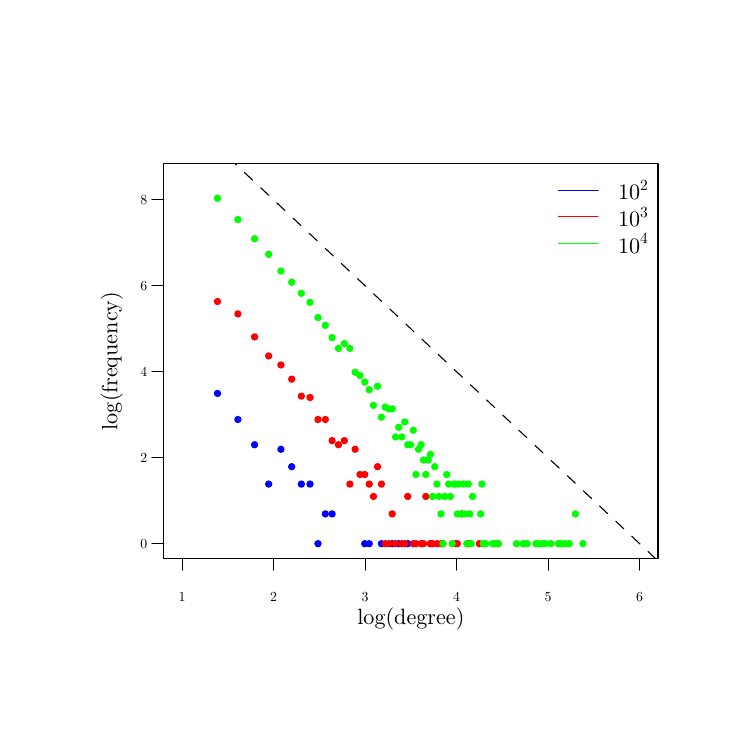
\begin{tikzpicture}[x=1pt,y=1pt]
\definecolor{fillColor}{RGB}{255,255,255}
\path[use as bounding box,fill=fillColor,fill opacity=0.00] (0,0) rectangle (252.94,252.94);
\begin{scope}
\path[clip] ( 49.20, 61.20) rectangle (227.75,203.75);
\definecolor{drawColor}{RGB}{0,0,255}
\definecolor{fillColor}{RGB}{0,0,255}

\path[draw=drawColor,line width= 0.4pt,line join=round,line cap=round,fill=fillColor] ( 68.59,120.77) circle (  1.12);

\path[draw=drawColor,line width= 0.4pt,line join=round,line cap=round,fill=fillColor] ( 75.96,111.36) circle (  1.12);

\path[draw=drawColor,line width= 0.4pt,line join=round,line cap=round,fill=fillColor] ( 81.99,102.23) circle (  1.12);

\path[draw=drawColor,line width= 0.4pt,line join=round,line cap=round,fill=fillColor] ( 87.09, 88.01) circle (  1.12);

\path[draw=drawColor,line width= 0.4pt,line join=round,line cap=round,fill=fillColor] ( 91.50,100.60) circle (  1.12);

\path[draw=drawColor,line width= 0.4pt,line join=round,line cap=round,fill=fillColor] ( 95.40, 94.30) circle (  1.12);

\path[draw=drawColor,line width= 0.4pt,line join=round,line cap=round,fill=fillColor] ( 98.88, 88.01) circle (  1.12);

\path[draw=drawColor,line width= 0.4pt,line join=round,line cap=round,fill=fillColor] (102.03, 88.01) circle (  1.12);

\path[draw=drawColor,line width= 0.4pt,line join=round,line cap=round,fill=fillColor] (104.91, 66.48) circle (  1.12);

\path[draw=drawColor,line width= 0.4pt,line join=round,line cap=round,fill=fillColor] (107.56, 77.24) circle (  1.12);

\path[draw=drawColor,line width= 0.4pt,line join=round,line cap=round,fill=fillColor] (110.01, 77.24) circle (  1.12);

\path[draw=drawColor,line width= 0.4pt,line join=round,line cap=round,fill=fillColor] (121.80, 66.48) circle (  1.12);

\path[draw=drawColor,line width= 0.4pt,line join=round,line cap=round,fill=fillColor] (123.41, 66.48) circle (  1.12);

\path[draw=drawColor,line width= 0.4pt,line join=round,line cap=round,fill=fillColor] (127.83, 66.48) circle (  1.12);

\path[draw=drawColor,line width= 0.4pt,line join=round,line cap=round,fill=fillColor] (131.72, 66.48) circle (  1.12);

\path[draw=drawColor,line width= 0.4pt,line join=round,line cap=round,fill=fillColor] (134.08, 66.48) circle (  1.12);

\path[draw=drawColor,line width= 0.4pt,line join=round,line cap=round,fill=fillColor] (137.34, 66.48) circle (  1.12);

\path[draw=drawColor,line width= 0.4pt,line join=round,line cap=round,fill=fillColor] (145.53, 66.48) circle (  1.12);
\end{scope}
\begin{scope}
\path[clip] (  0.00,  0.00) rectangle (252.94,252.94);
\definecolor{drawColor}{RGB}{0,0,0}

\path[draw=drawColor,line width= 0.4pt,line join=round,line cap=round] ( 55.81, 61.20) -- (221.13, 61.20);

\path[draw=drawColor,line width= 0.4pt,line join=round,line cap=round] ( 55.81, 61.20) -- ( 55.81, 56.92);

\path[draw=drawColor,line width= 0.4pt,line join=round,line cap=round] ( 88.88, 61.20) -- ( 88.88, 56.92);

\path[draw=drawColor,line width= 0.4pt,line join=round,line cap=round] (121.94, 61.20) -- (121.94, 56.92);

\path[draw=drawColor,line width= 0.4pt,line join=round,line cap=round] (155.00, 61.20) -- (155.00, 56.92);

\path[draw=drawColor,line width= 0.4pt,line join=round,line cap=round] (188.07, 61.20) -- (188.07, 56.92);

\path[draw=drawColor,line width= 0.4pt,line join=round,line cap=round] (221.13, 61.20) -- (221.13, 56.92);

\node[text=drawColor,anchor=base,inner sep=0pt, outer sep=0pt, scale=  0.50] at ( 55.81, 45.60) {1};

\node[text=drawColor,anchor=base,inner sep=0pt, outer sep=0pt, scale=  0.50] at ( 88.88, 45.60) {2};

\node[text=drawColor,anchor=base,inner sep=0pt, outer sep=0pt, scale=  0.50] at (121.94, 45.60) {3};

\node[text=drawColor,anchor=base,inner sep=0pt, outer sep=0pt, scale=  0.50] at (155.00, 45.60) {4};

\node[text=drawColor,anchor=base,inner sep=0pt, outer sep=0pt, scale=  0.50] at (188.07, 45.60) {5};

\node[text=drawColor,anchor=base,inner sep=0pt, outer sep=0pt, scale=  0.50] at (221.13, 45.60) {6};

\path[draw=drawColor,line width= 0.4pt,line join=round,line cap=round] ( 49.20, 66.48) -- ( 49.20,190.70);

\path[draw=drawColor,line width= 0.4pt,line join=round,line cap=round] ( 49.20, 66.48) -- ( 44.92, 66.48);

\path[draw=drawColor,line width= 0.4pt,line join=round,line cap=round] ( 49.20, 97.53) -- ( 44.92, 97.53);

\path[draw=drawColor,line width= 0.4pt,line join=round,line cap=round] ( 49.20,128.59) -- ( 44.92,128.59);

\path[draw=drawColor,line width= 0.4pt,line join=round,line cap=round] ( 49.20,159.65) -- ( 44.92,159.65);

\path[draw=drawColor,line width= 0.4pt,line join=round,line cap=round] ( 49.20,190.70) -- ( 44.92,190.70);

\node[text=drawColor,anchor=base east,inner sep=0pt, outer sep=0pt, scale=  0.50] at ( 43.20, 64.76) {0};

\node[text=drawColor,anchor=base east,inner sep=0pt, outer sep=0pt, scale=  0.50] at ( 43.20, 95.81) {2};

\node[text=drawColor,anchor=base east,inner sep=0pt, outer sep=0pt, scale=  0.50] at ( 43.20,126.87) {4};

\node[text=drawColor,anchor=base east,inner sep=0pt, outer sep=0pt, scale=  0.50] at ( 43.20,157.92) {6};

\node[text=drawColor,anchor=base east,inner sep=0pt, outer sep=0pt, scale=  0.50] at ( 43.20,188.98) {8};

\path[draw=drawColor,line width= 0.4pt,line join=round,line cap=round] ( 49.20, 61.20) --
	(227.75, 61.20) --
	(227.75,203.75) --
	( 49.20,203.75) --
	( 49.20, 61.20);
\end{scope}
\begin{scope}
\path[clip] (  0.00,  0.00) rectangle (252.94,252.94);
\definecolor{drawColor}{RGB}{0,0,0}

\node[text=drawColor,anchor=base,inner sep=0pt, outer sep=0pt, scale=  0.80] at (138.47, 37.20) {log(degree)};

\node[text=drawColor,rotate= 90.00,anchor=base,inner sep=0pt, outer sep=0pt, scale=  0.80] at ( 32.40,132.47) {log(frequency)};
\end{scope}
\begin{scope}
\path[clip] ( 49.20, 61.20) rectangle (227.75,203.75);
\definecolor{drawColor}{RGB}{255,0,0}
\definecolor{fillColor}{RGB}{255,0,0}

\path[draw=drawColor,line width= 0.4pt,line join=round,line cap=round,fill=fillColor] ( 68.59,153.98) circle (  1.12);

\path[draw=drawColor,line width= 0.4pt,line join=round,line cap=round,fill=fillColor] ( 75.96,149.51) circle (  1.12);

\path[draw=drawColor,line width= 0.4pt,line join=round,line cap=round,fill=fillColor] ( 81.99,141.20) circle (  1.12);

\path[draw=drawColor,line width= 0.4pt,line join=round,line cap=round,fill=fillColor] ( 87.09,134.33) circle (  1.12);

\path[draw=drawColor,line width= 0.4pt,line join=round,line cap=round,fill=fillColor] ( 91.50,131.06) circle (  1.12);

\path[draw=drawColor,line width= 0.4pt,line join=round,line cap=round,fill=fillColor] ( 95.40,125.93) circle (  1.12);

\path[draw=drawColor,line width= 0.4pt,line join=round,line cap=round,fill=fillColor] ( 98.88,119.80) circle (  1.12);

\path[draw=drawColor,line width= 0.4pt,line join=round,line cap=round,fill=fillColor] (102.03,119.29) circle (  1.12);

\path[draw=drawColor,line width= 0.4pt,line join=round,line cap=round,fill=fillColor] (104.91,111.36) circle (  1.12);

\path[draw=drawColor,line width= 0.4pt,line join=round,line cap=round,fill=fillColor] (107.56,111.36) circle (  1.12);

\path[draw=drawColor,line width= 0.4pt,line join=round,line cap=round,fill=fillColor] (110.01,103.71) circle (  1.12);

\path[draw=drawColor,line width= 0.4pt,line join=round,line cap=round,fill=fillColor] (112.29,102.23) circle (  1.12);

\path[draw=drawColor,line width= 0.4pt,line join=round,line cap=round,fill=fillColor] (114.42,103.71) circle (  1.12);

\path[draw=drawColor,line width= 0.4pt,line join=round,line cap=round,fill=fillColor] (116.43, 88.01) circle (  1.12);

\path[draw=drawColor,line width= 0.4pt,line join=round,line cap=round,fill=fillColor] (118.32,100.60) circle (  1.12);

\path[draw=drawColor,line width= 0.4pt,line join=round,line cap=round,fill=fillColor] (120.10, 91.47) circle (  1.12);

\path[draw=drawColor,line width= 0.4pt,line join=round,line cap=round,fill=fillColor] (121.80, 91.47) circle (  1.12);

\path[draw=drawColor,line width= 0.4pt,line join=round,line cap=round,fill=fillColor] (123.41, 88.01) circle (  1.12);

\path[draw=drawColor,line width= 0.4pt,line join=round,line cap=round,fill=fillColor] (124.95, 83.54) circle (  1.12);

\path[draw=drawColor,line width= 0.4pt,line join=round,line cap=round,fill=fillColor] (126.42, 94.30) circle (  1.12);

\path[draw=drawColor,line width= 0.4pt,line join=round,line cap=round,fill=fillColor] (127.83, 88.01) circle (  1.12);

\path[draw=drawColor,line width= 0.4pt,line join=round,line cap=round,fill=fillColor] (129.18, 66.48) circle (  1.12);

\path[draw=drawColor,line width= 0.4pt,line join=round,line cap=round,fill=fillColor] (130.47, 66.48) circle (  1.12);

\path[draw=drawColor,line width= 0.4pt,line join=round,line cap=round,fill=fillColor] (131.72, 77.24) circle (  1.12);

\path[draw=drawColor,line width= 0.4pt,line join=round,line cap=round,fill=fillColor] (132.92, 66.48) circle (  1.12);

\path[draw=drawColor,line width= 0.4pt,line join=round,line cap=round,fill=fillColor] (135.21, 66.48) circle (  1.12);

\path[draw=drawColor,line width= 0.4pt,line join=round,line cap=round,fill=fillColor] (136.29, 66.48) circle (  1.12);

\path[draw=drawColor,line width= 0.4pt,line join=round,line cap=round,fill=fillColor] (137.34, 83.54) circle (  1.12);

\path[draw=drawColor,line width= 0.4pt,line join=round,line cap=round,fill=fillColor] (139.34, 66.48) circle (  1.12);

\path[draw=drawColor,line width= 0.4pt,line join=round,line cap=round,fill=fillColor] (140.30, 66.48) circle (  1.12);

\path[draw=drawColor,line width= 0.4pt,line join=round,line cap=round,fill=fillColor] (142.14, 66.48) circle (  1.12);

\path[draw=drawColor,line width= 0.4pt,line join=round,line cap=round,fill=fillColor] (143.02, 66.48) circle (  1.12);

\path[draw=drawColor,line width= 0.4pt,line join=round,line cap=round,fill=fillColor] (143.88, 83.54) circle (  1.12);

\path[draw=drawColor,line width= 0.4pt,line join=round,line cap=round,fill=fillColor] (145.53, 66.48) circle (  1.12);

\path[draw=drawColor,line width= 0.4pt,line join=round,line cap=round,fill=fillColor] (146.33, 66.48) circle (  1.12);

\path[draw=drawColor,line width= 0.4pt,line join=round,line cap=round,fill=fillColor] (147.87, 66.48) circle (  1.12);

\path[draw=drawColor,line width= 0.4pt,line join=round,line cap=round,fill=fillColor] (149.34, 66.48) circle (  1.12);

\path[draw=drawColor,line width= 0.4pt,line join=round,line cap=round,fill=fillColor] (150.05, 66.48) circle (  1.12);

\path[draw=drawColor,line width= 0.4pt,line join=round,line cap=round,fill=fillColor] (154.64, 66.48) circle (  1.12);

\path[draw=drawColor,line width= 0.4pt,line join=round,line cap=round,fill=fillColor] (155.25, 66.48) circle (  1.12);

\path[draw=drawColor,line width= 0.4pt,line join=round,line cap=round,fill=fillColor] (157.00, 77.24) circle (  1.12);

\path[draw=drawColor,line width= 0.4pt,line join=round,line cap=round,fill=fillColor] (159.21, 66.48) circle (  1.12);

\path[draw=drawColor,line width= 0.4pt,line join=round,line cap=round,fill=fillColor] (163.22, 66.48) circle (  1.12);

\path[draw=drawColor,line width= 0.4pt,line join=round,line cap=round,fill=fillColor] (170.03, 66.48) circle (  1.12);
\end{scope}
\begin{scope}
\path[clip] ( 49.20, 61.20) rectangle (227.75,203.75);
\definecolor{drawColor}{RGB}{0,255,0}
\definecolor{fillColor}{RGB}{0,255,0}

\path[draw=drawColor,line width= 0.4pt,line join=round,line cap=round,fill=fillColor] ( 68.59,191.30) circle (  1.12);

\path[draw=drawColor,line width= 0.4pt,line join=round,line cap=round,fill=fillColor] ( 75.96,183.61) circle (  1.12);

\path[draw=drawColor,line width= 0.4pt,line join=round,line cap=round,fill=fillColor] ( 81.99,176.65) circle (  1.12);

\path[draw=drawColor,line width= 0.4pt,line join=round,line cap=round,fill=fillColor] ( 87.09,171.05) circle (  1.12);

\path[draw=drawColor,line width= 0.4pt,line join=round,line cap=round,fill=fillColor] ( 91.50,165.01) circle (  1.12);

\path[draw=drawColor,line width= 0.4pt,line join=round,line cap=round,fill=fillColor] ( 95.40,160.96) circle (  1.12);

\path[draw=drawColor,line width= 0.4pt,line join=round,line cap=round,fill=fillColor] ( 98.88,156.94) circle (  1.12);

\path[draw=drawColor,line width= 0.4pt,line join=round,line cap=round,fill=fillColor] (102.03,153.70) circle (  1.12);

\path[draw=drawColor,line width= 0.4pt,line join=round,line cap=round,fill=fillColor] (104.91,148.20) circle (  1.12);

\path[draw=drawColor,line width= 0.4pt,line join=round,line cap=round,fill=fillColor] (107.56,145.38) circle (  1.12);

\path[draw=drawColor,line width= 0.4pt,line join=round,line cap=round,fill=fillColor] (110.01,140.95) circle (  1.12);

\path[draw=drawColor,line width= 0.4pt,line join=round,line cap=round,fill=fillColor] (112.29,137.03) circle (  1.12);

\path[draw=drawColor,line width= 0.4pt,line join=round,line cap=round,fill=fillColor] (114.42,138.75) circle (  1.12);

\path[draw=drawColor,line width= 0.4pt,line join=round,line cap=round,fill=fillColor] (116.43,137.03) circle (  1.12);

\path[draw=drawColor,line width= 0.4pt,line join=round,line cap=round,fill=fillColor] (118.32,128.42) circle (  1.12);

\path[draw=drawColor,line width= 0.4pt,line join=round,line cap=round,fill=fillColor] (120.10,127.22) circle (  1.12);

\path[draw=drawColor,line width= 0.4pt,line join=round,line cap=round,fill=fillColor] (121.80,124.88) circle (  1.12);

\path[draw=drawColor,line width= 0.4pt,line join=round,line cap=round,fill=fillColor] (123.41,122.12) circle (  1.12);

\path[draw=drawColor,line width= 0.4pt,line join=round,line cap=round,fill=fillColor] (124.95,116.46) circle (  1.12);

\path[draw=drawColor,line width= 0.4pt,line join=round,line cap=round,fill=fillColor] (126.42,123.37) circle (  1.12);

\path[draw=drawColor,line width= 0.4pt,line join=round,line cap=round,fill=fillColor] (127.83,112.20) circle (  1.12);

\path[draw=drawColor,line width= 0.4pt,line join=round,line cap=round,fill=fillColor] (129.18,115.83) circle (  1.12);

\path[draw=drawColor,line width= 0.4pt,line join=round,line cap=round,fill=fillColor] (130.47,115.17) circle (  1.12);

\path[draw=drawColor,line width= 0.4pt,line join=round,line cap=round,fill=fillColor] (131.72,115.17) circle (  1.12);

\path[draw=drawColor,line width= 0.4pt,line join=round,line cap=round,fill=fillColor] (132.92,105.06) circle (  1.12);

\path[draw=drawColor,line width= 0.4pt,line join=round,line cap=round,fill=fillColor] (134.08,108.53) circle (  1.12);

\path[draw=drawColor,line width= 0.4pt,line join=round,line cap=round,fill=fillColor] (135.21,105.06) circle (  1.12);

\path[draw=drawColor,line width= 0.4pt,line join=round,line cap=round,fill=fillColor] (136.29,110.47) circle (  1.12);

\path[draw=drawColor,line width= 0.4pt,line join=round,line cap=round,fill=fillColor] (137.34,102.23) circle (  1.12);

\path[draw=drawColor,line width= 0.4pt,line join=round,line cap=round,fill=fillColor] (138.36,102.23) circle (  1.12);

\path[draw=drawColor,line width= 0.4pt,line join=round,line cap=round,fill=fillColor] (139.34,107.46) circle (  1.12);

\path[draw=drawColor,line width= 0.4pt,line join=round,line cap=round,fill=fillColor] (140.30, 91.47) circle (  1.12);

\path[draw=drawColor,line width= 0.4pt,line join=round,line cap=round,fill=fillColor] (141.23,100.60) circle (  1.12);

\path[draw=drawColor,line width= 0.4pt,line join=round,line cap=round,fill=fillColor] (142.14,102.23) circle (  1.12);

\path[draw=drawColor,line width= 0.4pt,line join=round,line cap=round,fill=fillColor] (143.02, 96.70) circle (  1.12);

\path[draw=drawColor,line width= 0.4pt,line join=round,line cap=round,fill=fillColor] (143.88, 91.47) circle (  1.12);

\path[draw=drawColor,line width= 0.4pt,line join=round,line cap=round,fill=fillColor] (144.72, 96.70) circle (  1.12);

\path[draw=drawColor,line width= 0.4pt,line join=round,line cap=round,fill=fillColor] (145.53, 98.77) circle (  1.12);

\path[draw=drawColor,line width= 0.4pt,line join=round,line cap=round,fill=fillColor] (146.33, 83.54) circle (  1.12);

\path[draw=drawColor,line width= 0.4pt,line join=round,line cap=round,fill=fillColor] (147.11, 94.30) circle (  1.12);

\path[draw=drawColor,line width= 0.4pt,line join=round,line cap=round,fill=fillColor] (147.87, 88.01) circle (  1.12);

\path[draw=drawColor,line width= 0.4pt,line join=round,line cap=round,fill=fillColor] (148.61, 83.54) circle (  1.12);

\path[draw=drawColor,line width= 0.4pt,line join=round,line cap=round,fill=fillColor] (149.34, 77.24) circle (  1.12);

\path[draw=drawColor,line width= 0.4pt,line join=round,line cap=round,fill=fillColor] (150.05, 66.48) circle (  1.12);

\path[draw=drawColor,line width= 0.4pt,line join=round,line cap=round,fill=fillColor] (150.75, 83.54) circle (  1.12);

\path[draw=drawColor,line width= 0.4pt,line join=round,line cap=round,fill=fillColor] (151.43, 91.47) circle (  1.12);

\path[draw=drawColor,line width= 0.4pt,line join=round,line cap=round,fill=fillColor] (152.10, 88.01) circle (  1.12);

\path[draw=drawColor,line width= 0.4pt,line join=round,line cap=round,fill=fillColor] (152.75, 83.54) circle (  1.12);

\path[draw=drawColor,line width= 0.4pt,line join=round,line cap=round,fill=fillColor] (153.39, 66.48) circle (  1.12);

\path[draw=drawColor,line width= 0.4pt,line join=round,line cap=round,fill=fillColor] (154.02, 88.01) circle (  1.12);

\path[draw=drawColor,line width= 0.4pt,line join=round,line cap=round,fill=fillColor] (154.64, 88.01) circle (  1.12);

\path[draw=drawColor,line width= 0.4pt,line join=round,line cap=round,fill=fillColor] (155.25, 77.24) circle (  1.12);

\path[draw=drawColor,line width= 0.4pt,line join=round,line cap=round,fill=fillColor] (155.84, 88.01) circle (  1.12);

\path[draw=drawColor,line width= 0.4pt,line join=round,line cap=round,fill=fillColor] (156.43, 77.24) circle (  1.12);

\path[draw=drawColor,line width= 0.4pt,line join=round,line cap=round,fill=fillColor] (157.57, 88.01) circle (  1.12);

\path[draw=drawColor,line width= 0.4pt,line join=round,line cap=round,fill=fillColor] (158.12, 77.24) circle (  1.12);

\path[draw=drawColor,line width= 0.4pt,line join=round,line cap=round,fill=fillColor] (158.67, 66.48) circle (  1.12);

\path[draw=drawColor,line width= 0.4pt,line join=round,line cap=round,fill=fillColor] (159.21, 88.01) circle (  1.12);

\path[draw=drawColor,line width= 0.4pt,line join=round,line cap=round,fill=fillColor] (159.74, 77.24) circle (  1.12);

\path[draw=drawColor,line width= 0.4pt,line join=round,line cap=round,fill=fillColor] (160.26, 66.48) circle (  1.12);

\path[draw=drawColor,line width= 0.4pt,line join=round,line cap=round,fill=fillColor] (160.77, 83.54) circle (  1.12);

\path[draw=drawColor,line width= 0.4pt,line join=round,line cap=round,fill=fillColor] (163.69, 77.24) circle (  1.12);

\path[draw=drawColor,line width= 0.4pt,line join=round,line cap=round,fill=fillColor] (164.15, 88.01) circle (  1.12);

\path[draw=drawColor,line width= 0.4pt,line join=round,line cap=round,fill=fillColor] (164.61, 66.48) circle (  1.12);

\path[draw=drawColor,line width= 0.4pt,line join=round,line cap=round,fill=fillColor] (165.06, 66.48) circle (  1.12);

\path[draw=drawColor,line width= 0.4pt,line join=round,line cap=round,fill=fillColor] (165.50, 66.48) circle (  1.12);

\path[draw=drawColor,line width= 0.4pt,line join=round,line cap=round,fill=fillColor] (168.05, 66.48) circle (  1.12);

\path[draw=drawColor,line width= 0.4pt,line join=round,line cap=round,fill=fillColor] (168.85, 66.48) circle (  1.12);

\path[draw=drawColor,line width= 0.4pt,line join=round,line cap=round,fill=fillColor] (169.64, 66.48) circle (  1.12);

\path[draw=drawColor,line width= 0.4pt,line join=round,line cap=round,fill=fillColor] (170.03, 66.48) circle (  1.12);

\path[draw=drawColor,line width= 0.4pt,line join=round,line cap=round,fill=fillColor] (176.63, 66.48) circle (  1.12);

\path[draw=drawColor,line width= 0.4pt,line join=round,line cap=round,fill=fillColor] (179.05, 66.48) circle (  1.12);

\path[draw=drawColor,line width= 0.4pt,line join=round,line cap=round,fill=fillColor] (179.35, 66.48) circle (  1.12);

\path[draw=drawColor,line width= 0.4pt,line join=round,line cap=round,fill=fillColor] (180.49, 66.48) circle (  1.12);

\path[draw=drawColor,line width= 0.4pt,line join=round,line cap=round,fill=fillColor] (183.69, 66.48) circle (  1.12);

\path[draw=drawColor,line width= 0.4pt,line join=round,line cap=round,fill=fillColor] (184.19, 66.48) circle (  1.12);

\path[draw=drawColor,line width= 0.4pt,line join=round,line cap=round,fill=fillColor] (185.42, 66.48) circle (  1.12);

\path[draw=drawColor,line width= 0.4pt,line join=round,line cap=round,fill=fillColor] (186.37, 66.48) circle (  1.12);

\path[draw=drawColor,line width= 0.4pt,line join=round,line cap=round,fill=fillColor] (187.07, 66.48) circle (  1.12);

\path[draw=drawColor,line width= 0.4pt,line join=round,line cap=round,fill=fillColor] (189.07, 66.48) circle (  1.12);

\path[draw=drawColor,line width= 0.4pt,line join=round,line cap=round,fill=fillColor] (191.77, 66.48) circle (  1.12);

\path[draw=drawColor,line width= 0.4pt,line join=round,line cap=round,fill=fillColor] (192.75, 66.48) circle (  1.12);

\path[draw=drawColor,line width= 0.4pt,line join=round,line cap=round,fill=fillColor] (194.08, 66.48) circle (  1.12);

\path[draw=drawColor,line width= 0.4pt,line join=round,line cap=round,fill=fillColor] (194.26, 66.48) circle (  1.12);

\path[draw=drawColor,line width= 0.4pt,line join=round,line cap=round,fill=fillColor] (195.71, 66.48) circle (  1.12);

\path[draw=drawColor,line width= 0.4pt,line join=round,line cap=round,fill=fillColor] (197.93, 77.24) circle (  1.12);

\path[draw=drawColor,line width= 0.4pt,line join=round,line cap=round,fill=fillColor] (200.63, 66.48) circle (  1.12);
\end{scope}
\begin{scope}
\path[clip] ( 49.20, 61.20) rectangle (227.75,203.75);
\definecolor{drawColor}{RGB}{0,0,0}

\path[draw=drawColor,line width= 0.4pt,dash pattern=on 4pt off 4pt ,line join=round,line cap=round] ( 49.20,227.97) -- (227.75, 60.27);
\definecolor{drawColor}{RGB}{0,0,255}

\path[draw=drawColor,line width= 0.4pt,line join=round,line cap=round] (191.75,194.15) -- (206.15,194.15);
\definecolor{drawColor}{RGB}{255,0,0}

\path[draw=drawColor,line width= 0.4pt,line join=round,line cap=round] (191.75,184.55) -- (206.15,184.55);
\definecolor{drawColor}{RGB}{0,255,0}

\path[draw=drawColor,line width= 0.4pt,line join=round,line cap=round] (191.75,174.95) -- (206.15,174.95);
\definecolor{drawColor}{RGB}{0,0,0}

\node[text=drawColor,anchor=base west,inner sep=0pt, outer sep=0pt, scale=  0.80] at (213.35,190.71) {10};

\node[text=drawColor,anchor=base west,inner sep=0pt, outer sep=0pt, scale=  0.56] at (221.35,193.98) {2};

\node[text=drawColor,anchor=base west,inner sep=0pt, outer sep=0pt, scale=  0.80] at (213.35,181.11) {10};

\node[text=drawColor,anchor=base west,inner sep=0pt, outer sep=0pt, scale=  0.56] at (221.35,184.38) {3};

\node[text=drawColor,anchor=base west,inner sep=0pt, outer sep=0pt, scale=  0.80] at (213.35,171.51) {10};

\node[text=drawColor,anchor=base west,inner sep=0pt, outer sep=0pt, scale=  0.56] at (221.35,174.78) {4};
\end{scope}
\end{tikzpicture}
 
\end{tabular}
\caption{Degree Distribution}
\label{p01}
\end{figure}

\pagebreak
\subsection*{(c)}

\begin{figure}[!htb]
	\begin{tabular}{cc}
		% Created by tikzDevice version 0.10.1 on 2016-06-15 03:03:14
% !TEX encoding = UTF-8 Unicode
\begin{tikzpicture}[x=1pt,y=1pt]
\definecolor{fillColor}{RGB}{255,255,255}
\path[use as bounding box,fill=fillColor,fill opacity=0.00] (0,0) rectangle (252.94,252.94);
\begin{scope}
\path[clip] ( 49.20, 61.20) rectangle (227.75,203.75);
\definecolor{drawColor}{RGB}{0,0,255}

\path[draw=drawColor,line width= 0.4pt,line join=round,line cap=round] ( 55.81,102.12) --
	( 63.00,120.59) --
	( 70.19,141.71) --
	( 77.38,154.91) --
	( 84.56,161.51) --
	( 91.75,169.43) --
	( 98.94,173.39) --
	(106.13,176.03) --
	(120.50,182.63) --
	(127.69,183.95) --
	(134.88,186.59) --
	(142.07,189.23) --
	(149.25,190.55) --
	(156.44,191.87) --
	(170.82,193.19) --
	(178.01,194.51) --
	(192.38,197.15) --
	(221.13,198.47);
\end{scope}
\begin{scope}
\path[clip] (  0.00,  0.00) rectangle (252.94,252.94);
\definecolor{drawColor}{RGB}{0,0,0}

\path[draw=drawColor,line width= 0.4pt,line join=round,line cap=round] ( 63.00, 61.20) -- (206.76, 61.20);

\path[draw=drawColor,line width= 0.4pt,line join=round,line cap=round] ( 63.00, 61.20) -- ( 63.00, 56.92);

\path[draw=drawColor,line width= 0.4pt,line join=round,line cap=round] ( 98.94, 61.20) -- ( 98.94, 56.92);

\path[draw=drawColor,line width= 0.4pt,line join=round,line cap=round] (134.88, 61.20) -- (134.88, 56.92);

\path[draw=drawColor,line width= 0.4pt,line join=round,line cap=round] (170.82, 61.20) -- (170.82, 56.92);

\path[draw=drawColor,line width= 0.4pt,line join=round,line cap=round] (206.76, 61.20) -- (206.76, 56.92);

\node[text=drawColor,anchor=base,inner sep=0pt, outer sep=0pt, scale=  0.50] at ( 63.00, 45.60) {5};

\node[text=drawColor,anchor=base,inner sep=0pt, outer sep=0pt, scale=  0.50] at ( 98.94, 45.60) {10};

\node[text=drawColor,anchor=base,inner sep=0pt, outer sep=0pt, scale=  0.50] at (134.88, 45.60) {15};

\node[text=drawColor,anchor=base,inner sep=0pt, outer sep=0pt, scale=  0.50] at (170.82, 45.60) {20};

\node[text=drawColor,anchor=base,inner sep=0pt, outer sep=0pt, scale=  0.50] at (206.76, 45.60) {25};

\path[draw=drawColor,line width= 0.4pt,line join=round,line cap=round] ( 49.20, 66.48) -- ( 49.20,198.47);

\path[draw=drawColor,line width= 0.4pt,line join=round,line cap=round] ( 49.20, 66.48) -- ( 44.92, 66.48);

\path[draw=drawColor,line width= 0.4pt,line join=round,line cap=round] ( 49.20, 92.88) -- ( 44.92, 92.88);

\path[draw=drawColor,line width= 0.4pt,line join=round,line cap=round] ( 49.20,119.27) -- ( 44.92,119.27);

\path[draw=drawColor,line width= 0.4pt,line join=round,line cap=round] ( 49.20,145.67) -- ( 44.92,145.67);

\path[draw=drawColor,line width= 0.4pt,line join=round,line cap=round] ( 49.20,172.07) -- ( 44.92,172.07);

\path[draw=drawColor,line width= 0.4pt,line join=round,line cap=round] ( 49.20,198.47) -- ( 44.92,198.47);

\node[text=drawColor,anchor=base east,inner sep=0pt, outer sep=0pt, scale=  0.50] at ( 43.20, 64.76) {0.0};

\node[text=drawColor,anchor=base east,inner sep=0pt, outer sep=0pt, scale=  0.50] at ( 43.20, 91.15) {0.2};

\node[text=drawColor,anchor=base east,inner sep=0pt, outer sep=0pt, scale=  0.50] at ( 43.20,117.55) {0.4};

\node[text=drawColor,anchor=base east,inner sep=0pt, outer sep=0pt, scale=  0.50] at ( 43.20,143.95) {0.6};

\node[text=drawColor,anchor=base east,inner sep=0pt, outer sep=0pt, scale=  0.50] at ( 43.20,170.35) {0.8};

\node[text=drawColor,anchor=base east,inner sep=0pt, outer sep=0pt, scale=  0.50] at ( 43.20,196.74) {1.0};

\path[draw=drawColor,line width= 0.4pt,line join=round,line cap=round] ( 49.20,203.75) --
	( 49.20, 61.20) --
	(227.75, 61.20);
\end{scope}
\end{tikzpicture}
 & % Created by tikzDevice version 0.10.1 on 2016-06-15 03:03:14
% !TEX encoding = UTF-8 Unicode
\begin{tikzpicture}[x=1pt,y=1pt]
\definecolor{fillColor}{RGB}{255,255,255}
\path[use as bounding box,fill=fillColor,fill opacity=0.00] (0,0) rectangle (252.94,252.94);
\begin{scope}
\path[clip] ( 49.20, 61.20) rectangle (227.75,203.75);
\definecolor{drawColor}{RGB}{255,0,0}

\path[draw=drawColor,line width= 0.4pt,line join=round,line cap=round] ( 55.81,107.66) --
	( 57.88,133.13) --
	( 59.95,149.89) --
	( 62.01,158.74) --
	( 64.08,166.92) --
	( 66.15,172.20) --
	( 68.21,176.69) --
	( 70.28,181.04) --
	( 72.34,183.16) --
	( 74.41,185.53) --
	( 76.48,187.64) --
	( 78.54,188.57) --
	( 80.61,189.23) --
	( 82.68,190.02) --
	( 84.74,190.68) --
	( 86.81,192.00) --
	( 88.88,192.53) --
	( 90.94,192.92) --
	( 93.01,193.19) --
	( 95.08,193.58) --
	( 97.14,193.85) --
	( 99.21,194.11) --
	(101.28,194.64) --
	(103.34,194.77) --
	(105.41,195.17) --
	(107.48,195.56) --
	(111.61,195.83) --
	(115.74,196.35) --
	(117.81,196.49) --
	(121.94,196.62) --
	(124.01,196.75) --
	(130.21,196.88) --
	(136.41,197.01) --
	(142.61,197.15) --
	(144.67,197.28) --
	(146.74,197.41) --
	(150.87,197.54) --
	(169.47,197.67) --
	(188.07,197.81) --
	(198.40,197.94) --
	(210.80,198.07) --
	(219.07,198.33) --
	(221.13,198.47);
\end{scope}
\begin{scope}
\path[clip] (  0.00,  0.00) rectangle (252.94,252.94);
\definecolor{drawColor}{RGB}{0,0,0}

\path[draw=drawColor,line width= 0.4pt,line join=round,line cap=round] ( 88.88, 61.20) -- (212.87, 61.20);

\path[draw=drawColor,line width= 0.4pt,line join=round,line cap=round] ( 88.88, 61.20) -- ( 88.88, 56.92);

\path[draw=drawColor,line width= 0.4pt,line join=round,line cap=round] (130.21, 61.20) -- (130.21, 56.92);

\path[draw=drawColor,line width= 0.4pt,line join=round,line cap=round] (171.54, 61.20) -- (171.54, 56.92);

\path[draw=drawColor,line width= 0.4pt,line join=round,line cap=round] (212.87, 61.20) -- (212.87, 56.92);

\node[text=drawColor,anchor=base,inner sep=0pt, outer sep=0pt, scale=  0.50] at ( 88.88, 45.60) {20};

\node[text=drawColor,anchor=base,inner sep=0pt, outer sep=0pt, scale=  0.50] at (130.21, 45.60) {40};

\node[text=drawColor,anchor=base,inner sep=0pt, outer sep=0pt, scale=  0.50] at (171.54, 45.60) {60};

\node[text=drawColor,anchor=base,inner sep=0pt, outer sep=0pt, scale=  0.50] at (212.87, 45.60) {80};

\path[draw=drawColor,line width= 0.4pt,line join=round,line cap=round] ( 49.20, 66.48) -- ( 49.20,198.47);

\path[draw=drawColor,line width= 0.4pt,line join=round,line cap=round] ( 49.20, 66.48) -- ( 44.92, 66.48);

\path[draw=drawColor,line width= 0.4pt,line join=round,line cap=round] ( 49.20, 92.88) -- ( 44.92, 92.88);

\path[draw=drawColor,line width= 0.4pt,line join=round,line cap=round] ( 49.20,119.27) -- ( 44.92,119.27);

\path[draw=drawColor,line width= 0.4pt,line join=round,line cap=round] ( 49.20,145.67) -- ( 44.92,145.67);

\path[draw=drawColor,line width= 0.4pt,line join=round,line cap=round] ( 49.20,172.07) -- ( 44.92,172.07);

\path[draw=drawColor,line width= 0.4pt,line join=round,line cap=round] ( 49.20,198.47) -- ( 44.92,198.47);

\node[text=drawColor,anchor=base east,inner sep=0pt, outer sep=0pt, scale=  0.50] at ( 43.20, 64.76) {0.0};

\node[text=drawColor,anchor=base east,inner sep=0pt, outer sep=0pt, scale=  0.50] at ( 43.20, 91.15) {0.2};

\node[text=drawColor,anchor=base east,inner sep=0pt, outer sep=0pt, scale=  0.50] at ( 43.20,117.55) {0.4};

\node[text=drawColor,anchor=base east,inner sep=0pt, outer sep=0pt, scale=  0.50] at ( 43.20,143.95) {0.6};

\node[text=drawColor,anchor=base east,inner sep=0pt, outer sep=0pt, scale=  0.50] at ( 43.20,170.35) {0.8};

\node[text=drawColor,anchor=base east,inner sep=0pt, outer sep=0pt, scale=  0.50] at ( 43.20,196.74) {1.0};

\path[draw=drawColor,line width= 0.4pt,line join=round,line cap=round] ( 49.20,203.75) --
	( 49.20, 61.20) --
	(227.75, 61.20);
\end{scope}
\end{tikzpicture}
 \\
		(a) CDF for $10^2$ nodes & (b) CDF for $10^3$ nodes \\
		 	% Created by tikzDevice version 0.10.1 on 2016-06-15 03:03:13
% !TEX encoding = UTF-8 Unicode
\begin{tikzpicture}[x=1pt,y=1pt]
\definecolor{fillColor}{RGB}{255,255,255}
\path[use as bounding box,fill=fillColor,fill opacity=0.00] (0,0) rectangle (252.94,252.94);
\begin{scope}
\path[clip] ( 49.20, 61.20) rectangle (227.75,203.75);
\definecolor{drawColor}{RGB}{0,255,0}

\path[draw=drawColor,line width= 0.4pt,line join=round,line cap=round] ( 55.81,106.60) --
	( 56.60,132.38) --
	( 57.39,147.82) --
	( 58.19,158.51) --
	( 58.98,166.34) --
	( 59.77,172.21) --
	( 60.56,177.11) --
	( 61.35,180.69) --
	( 62.14,183.45) --
	( 62.93,185.52) --
	( 63.72,187.37) --
	( 64.51,188.91) --
	( 65.30,189.97) --
	( 66.10,190.89) --
	( 66.89,191.50) --
	( 67.68,192.25) --
	( 68.47,192.92) --
	( 69.26,193.38) --
	( 70.05,193.82) --
	( 70.84,194.23) --
	( 71.63,194.53) --
	( 72.42,194.84) --
	( 73.21,195.01) --
	( 74.01,195.25) --
	( 74.80,195.50) --
	( 75.59,195.68) --
	( 76.38,195.87) --
	( 77.17,196.02) --
	( 77.96,196.23) --
	( 78.75,196.33) --
	( 79.54,196.43) --
	( 80.33,196.54) --
	( 81.12,196.71) --
	( 81.92,196.79) --
	( 82.71,196.96) --
	( 83.50,197.01) --
	( 84.29,197.12) --
	( 85.08,197.20) --
	( 85.87,197.24) --
	( 86.66,197.26) --
	( 87.45,197.34) --
	( 88.24,197.41) --
	( 89.03,197.44) --
	( 89.83,197.45) --
	( 90.62,197.46) --
	( 91.41,197.52) --
	( 92.20,197.55) --
	( 92.99,197.57) --
	( 93.78,197.62) --
	( 94.57,197.65) --
	( 95.36,197.67) --
	( 96.15,197.71) --
	( 96.94,197.74) --
	( 97.74,197.78) --
	( 98.53,197.83) --
	( 99.32,197.86) --
	(100.11,197.90) --
	(100.90,197.91) --
	(101.69,197.92) --
	(103.27,197.95) --
	(104.06,197.98) --
	(106.44,197.99) --
	(107.23,198.00) --
	(108.81,198.03) --
	(109.60,198.04) --
	(110.39,198.07) --
	(113.56,198.10) --
	(114.35,198.12) --
	(115.14,198.14) --
	(115.93,198.16) --
	(117.51,198.18) --
	(118.30,198.19) --
	(119.09,198.20) --
	(127.00,198.21) --
	(128.58,198.23) --
	(131.75,198.24) --
	(133.33,198.25) --
	(136.49,198.27) --
	(138.87,198.28) --
	(144.41,198.29) --
	(147.57,198.31) --
	(149.94,198.32) --
	(150.73,198.33) --
	(153.11,198.35) --
	(158.64,198.36) --
	(172.09,198.37) --
	(183.16,198.39) --
	(184.75,198.40) --
	(199.78,198.41) --
	(206.10,198.43) --
	(215.60,198.44) --
	(218.76,198.45) --
	(221.13,198.47);
\end{scope}
\begin{scope}
\path[clip] (  0.00,  0.00) rectangle (252.94,252.94);
\definecolor{drawColor}{RGB}{0,0,0}

\path[draw=drawColor,line width= 0.4pt,line join=round,line cap=round] ( 52.65, 61.20) -- (210.85, 61.20);

\path[draw=drawColor,line width= 0.4pt,line join=round,line cap=round] ( 52.65, 61.20) -- ( 52.65, 56.92);

\path[draw=drawColor,line width= 0.4pt,line join=round,line cap=round] ( 92.20, 61.20) -- ( 92.20, 56.92);

\path[draw=drawColor,line width= 0.4pt,line join=round,line cap=round] (131.75, 61.20) -- (131.75, 56.92);

\path[draw=drawColor,line width= 0.4pt,line join=round,line cap=round] (171.30, 61.20) -- (171.30, 56.92);

\path[draw=drawColor,line width= 0.4pt,line join=round,line cap=round] (210.85, 61.20) -- (210.85, 56.92);

\node[text=drawColor,anchor=base,inner sep=0pt, outer sep=0pt, scale=  0.50] at ( 52.65, 45.60) {0};

\node[text=drawColor,anchor=base,inner sep=0pt, outer sep=0pt, scale=  0.50] at ( 92.20, 45.60) {50};

\node[text=drawColor,anchor=base,inner sep=0pt, outer sep=0pt, scale=  0.50] at (131.75, 45.60) {100};

\node[text=drawColor,anchor=base,inner sep=0pt, outer sep=0pt, scale=  0.50] at (171.30, 45.60) {150};

\node[text=drawColor,anchor=base,inner sep=0pt, outer sep=0pt, scale=  0.50] at (210.85, 45.60) {200};

\path[draw=drawColor,line width= 0.4pt,line join=round,line cap=round] ( 49.20, 66.48) -- ( 49.20,198.47);

\path[draw=drawColor,line width= 0.4pt,line join=round,line cap=round] ( 49.20, 66.48) -- ( 44.92, 66.48);

\path[draw=drawColor,line width= 0.4pt,line join=round,line cap=round] ( 49.20, 92.88) -- ( 44.92, 92.88);

\path[draw=drawColor,line width= 0.4pt,line join=round,line cap=round] ( 49.20,119.27) -- ( 44.92,119.27);

\path[draw=drawColor,line width= 0.4pt,line join=round,line cap=round] ( 49.20,145.67) -- ( 44.92,145.67);

\path[draw=drawColor,line width= 0.4pt,line join=round,line cap=round] ( 49.20,172.07) -- ( 44.92,172.07);

\path[draw=drawColor,line width= 0.4pt,line join=round,line cap=round] ( 49.20,198.47) -- ( 44.92,198.47);

\node[text=drawColor,anchor=base east,inner sep=0pt, outer sep=0pt, scale=  0.50] at ( 43.20, 64.76) {0.0};

\node[text=drawColor,anchor=base east,inner sep=0pt, outer sep=0pt, scale=  0.50] at ( 43.20, 91.15) {0.2};

\node[text=drawColor,anchor=base east,inner sep=0pt, outer sep=0pt, scale=  0.50] at ( 43.20,117.55) {0.4};

\node[text=drawColor,anchor=base east,inner sep=0pt, outer sep=0pt, scale=  0.50] at ( 43.20,143.95) {0.6};

\node[text=drawColor,anchor=base east,inner sep=0pt, outer sep=0pt, scale=  0.50] at ( 43.20,170.35) {0.8};

\node[text=drawColor,anchor=base east,inner sep=0pt, outer sep=0pt, scale=  0.50] at ( 43.20,196.74) {1.0};

\path[draw=drawColor,line width= 0.4pt,line join=round,line cap=round] ( 49.20,203.75) --
	( 49.20, 61.20) --
	(227.75, 61.20);
\end{scope}
\end{tikzpicture}
 & \\
		 (c) CDF for $10^4$	nodes
	\end{tabular}
	\caption{Cumulative distribution function}
\end{figure}

\pagebreak
\subsection*{(d)}

\begin{table}[!htb]
	\centering
	\begin{tabular}{l|l}
		\toprule \toprule
		& Average Clustering Coefficient \\
		\hline
		\textbf{$10^2$} & 0.133 \\
		\textbf{$10^4$} & 0.03 \\ 
		\textbf{$10^6$} & 0.004 \\
		\hline 
		\bottomrule
	\end{tabular}
	\caption{Average clustering coefficient for intermediate steps}
\end{table}

\begin{figure}[!htb]
	\centering
	% Created by tikzDevice version 0.10.1 on 2016-06-15 03:24:18
% !TEX encoding = UTF-8 Unicode
\begin{tikzpicture}[x=1pt,y=1pt]
\definecolor{fillColor}{RGB}{255,255,255}
\path[use as bounding box,fill=fillColor,fill opacity=0.00] (0,0) rectangle (433.62,433.62);
\begin{scope}
\path[clip] ( 49.20, 61.20) rectangle (408.42,384.42);
\definecolor{drawColor}{RGB}{0,0,255}

\path[draw=drawColor,line width= 0.4pt,line join=round,line cap=round] ( 62.50,372.45) --
	( 65.82, 83.01) --
	( 69.14, 78.05) --
	( 72.47, 76.73) --
	( 75.80, 75.98) --
	( 79.12, 75.76) --
	( 82.45, 75.22) --
	( 85.77, 74.76) --
	( 89.10, 74.36) --
	( 92.43, 74.40) --
	( 95.75, 74.33) --
	( 99.08, 74.14) --
	(102.41, 74.13) --
	(105.73, 73.99) --
	(109.06, 74.04) --
	(112.38, 73.94) --
	(115.71, 73.97) --
	(119.04, 73.80) --
	(122.36, 73.80) --
	(125.69, 73.72) --
	(129.02, 73.85) --
	(132.34, 73.70) --
	(135.67, 73.66) --
	(138.99, 73.61) --
	(142.32, 73.63) --
	(145.65, 73.61) --
	(148.97, 73.61) --
	(152.30, 73.63) --
	(155.63, 73.52) --
	(158.95, 73.52) --
	(162.28, 73.48) --
	(165.60, 73.44) --
	(168.93, 73.51) --
	(172.26, 73.48) --
	(175.58, 73.43) --
	(178.91, 73.44) --
	(182.24, 73.45) --
	(185.56, 73.46) --
	(188.89, 73.45) --
	(192.21, 73.40) --
	(195.54, 73.39) --
	(198.87, 73.39) --
	(202.19, 73.42) --
	(205.52, 73.36) --
	(208.85, 73.37) --
	(212.17, 73.35) --
	(215.50, 73.33) --
	(218.82, 73.38) --
	(222.15, 73.35) --
	(225.48, 73.34) --
	(228.80, 73.36) --
	(232.13, 73.36) --
	(235.46, 73.28) --
	(238.78, 73.32) --
	(242.11, 73.34) --
	(245.43, 73.32) --
	(248.76, 73.30) --
	(252.09, 73.28) --
	(255.41, 73.28) --
	(258.74, 73.32) --
	(262.07, 73.28) --
	(265.39, 73.27) --
	(268.72, 73.28) --
	(272.04, 73.27) --
	(275.37, 73.26) --
	(278.70, 73.28) --
	(282.02, 73.25) --
	(285.35, 73.27) --
	(288.68, 73.24) --
	(292.00, 73.26) --
	(295.33, 73.28) --
	(298.65, 73.28) --
	(301.98, 73.25) --
	(305.31, 73.26) --
	(308.63, 73.23) --
	(311.96, 73.24) --
	(315.29, 73.26) --
	(318.61, 73.24) --
	(321.94, 73.24) --
	(325.26, 73.23) --
	(328.59, 73.22) --
	(331.92, 73.21) --
	(335.24, 73.21) --
	(338.57, 73.20) --
	(341.90, 73.21) --
	(345.22, 73.21) --
	(348.55, 73.19) --
	(351.87, 73.20) --
	(355.20, 73.19) --
	(358.53, 73.18) --
	(361.85, 73.19) --
	(365.18, 73.22) --
	(368.51, 73.21) --
	(371.83, 73.18) --
	(375.16, 73.19) --
	(378.48, 73.19) --
	(381.81, 73.18) --
	(385.14, 73.18) --
	(388.46, 73.17) --
	(391.79, 73.21) --
	(395.12, 73.17);
\end{scope}
\begin{scope}
\path[clip] (  0.00,  0.00) rectangle (433.62,433.62);
\definecolor{drawColor}{RGB}{0,0,0}

\path[draw=drawColor,line width= 0.4pt,line join=round,line cap=round] ( 62.49, 61.20) -- (395.12, 61.20);

\path[draw=drawColor,line width= 0.4pt,line join=round,line cap=round] ( 62.49, 61.20) -- ( 62.49, 57.97);

\path[draw=drawColor,line width= 0.4pt,line join=round,line cap=round] (129.02, 61.20) -- (129.02, 57.97);

\path[draw=drawColor,line width= 0.4pt,line join=round,line cap=round] (195.54, 61.20) -- (195.54, 57.97);

\path[draw=drawColor,line width= 0.4pt,line join=round,line cap=round] (262.07, 61.20) -- (262.07, 57.97);

\path[draw=drawColor,line width= 0.4pt,line join=round,line cap=round] (328.59, 61.20) -- (328.59, 57.97);

\path[draw=drawColor,line width= 0.4pt,line join=round,line cap=round] (395.12, 61.20) -- (395.12, 57.97);

\node[text=drawColor,anchor=base,inner sep=0pt, outer sep=0pt, scale=  0.50] at ( 62.49, 45.60) {0e+00};

\node[text=drawColor,anchor=base,inner sep=0pt, outer sep=0pt, scale=  0.50] at (129.02, 45.60) {2e+04};

\node[text=drawColor,anchor=base,inner sep=0pt, outer sep=0pt, scale=  0.50] at (195.54, 45.60) {4e+04};

\node[text=drawColor,anchor=base,inner sep=0pt, outer sep=0pt, scale=  0.50] at (262.07, 45.60) {6e+04};

\node[text=drawColor,anchor=base,inner sep=0pt, outer sep=0pt, scale=  0.50] at (328.59, 45.60) {8e+04};

\node[text=drawColor,anchor=base,inner sep=0pt, outer sep=0pt, scale=  0.50] at (395.12, 45.60) {1e+05};

\path[draw=drawColor,line width= 0.4pt,line join=round,line cap=round] ( 49.20, 73.01) -- ( 49.20,372.45);

\path[draw=drawColor,line width= 0.4pt,line join=round,line cap=round] ( 49.20, 73.01) -- ( 45.97, 73.01);

\path[draw=drawColor,line width= 0.4pt,line join=round,line cap=round] ( 49.20,132.90) -- ( 45.97,132.90);

\path[draw=drawColor,line width= 0.4pt,line join=round,line cap=round] ( 49.20,192.78) -- ( 45.97,192.78);

\path[draw=drawColor,line width= 0.4pt,line join=round,line cap=round] ( 49.20,252.67) -- ( 45.97,252.67);

\path[draw=drawColor,line width= 0.4pt,line join=round,line cap=round] ( 49.20,312.56) -- ( 45.97,312.56);

\path[draw=drawColor,line width= 0.4pt,line join=round,line cap=round] ( 49.20,372.45) -- ( 45.97,372.45);

\node[text=drawColor,anchor=base east,inner sep=0pt, outer sep=0pt, scale=  0.50] at ( 43.20, 71.29) {0.0};

\node[text=drawColor,anchor=base east,inner sep=0pt, outer sep=0pt, scale=  0.50] at ( 43.20,131.17) {0.2};

\node[text=drawColor,anchor=base east,inner sep=0pt, outer sep=0pt, scale=  0.50] at ( 43.20,191.06) {0.4};

\node[text=drawColor,anchor=base east,inner sep=0pt, outer sep=0pt, scale=  0.50] at ( 43.20,250.95) {0.6};

\node[text=drawColor,anchor=base east,inner sep=0pt, outer sep=0pt, scale=  0.50] at ( 43.20,310.84) {0.8};

\node[text=drawColor,anchor=base east,inner sep=0pt, outer sep=0pt, scale=  0.50] at ( 43.20,370.73) {1.0};

\path[draw=drawColor,line width= 0.4pt,line join=round,line cap=round] ( 49.20,384.42) --
	( 49.20, 61.20) --
	(408.42, 61.20);
\end{scope}
\begin{scope}
\path[clip] (  0.00,  0.00) rectangle (433.62,433.62);
\definecolor{drawColor}{RGB}{0,0,0}

\node[text=drawColor,anchor=base,inner sep=0pt, outer sep=0pt, scale=  0.80] at (228.81, 27.60) {N};

\node[text=drawColor,rotate= 90.00,anchor=base,inner sep=0pt, outer sep=0pt, scale=  0.80] at ( 22.80,222.81) {Average clustering coefficient};
\end{scope}
\end{tikzpicture}

	\caption{Average clustering coefficient as a function of N }
\end{figure}

\pagebreak
\subsection*{(e)}

\begin{figure}[!htb]
	\centering
	% Created by tikzDevice version 0.10.1 on 2016-06-15 03:37:23
% !TEX encoding = UTF-8 Unicode
\begin{tikzpicture}[x=1pt,y=1pt]
\definecolor{fillColor}{RGB}{255,255,255}
\path[use as bounding box,fill=fillColor,fill opacity=0.00] (0,0) rectangle (433.62,433.62);
\begin{scope}
\path[clip] ( 49.20, 61.20) rectangle (408.42,384.42);
\definecolor{drawColor}{RGB}{0,0,255}

\path[draw=drawColor,line width= 0.4pt,line join=round,line cap=round] ( 62.62, 81.72) --
	( 62.64, 81.72) --
	( 62.66, 83.86) --
	( 62.68, 83.86) --
	( 62.70, 86.00) --
	( 62.73, 88.13) --
	( 62.75, 88.13) --
	( 62.77, 88.13) --
	( 62.79, 88.13) --
	( 62.81, 90.27) --
	( 62.84, 90.27) --
	( 62.86, 90.27) --
	( 62.88, 90.27) --
	( 62.90, 92.41) --
	( 62.93, 92.41) --
	( 62.95, 92.41) --
	( 62.97, 92.41) --
	( 62.99, 92.41) --
	( 63.01, 92.41) --
	( 63.04, 94.55) --
	( 63.06, 94.55) --
	( 63.08, 94.55) --
	( 63.10, 94.55) --
	( 63.13, 94.55) --
	( 63.15, 94.55) --
	( 63.17, 94.55) --
	( 63.19, 94.55) --
	( 63.21, 94.55) --
	( 63.24, 94.55) --
	( 63.26, 94.55) --
	( 63.28, 94.55) --
	( 63.30, 94.55) --
	( 63.32, 94.55) --
	( 63.35, 94.55) --
	( 63.37, 94.55) --
	( 63.39, 94.55) --
	( 63.41, 96.69) --
	( 63.44, 96.69) --
	( 63.46, 96.69) --
	( 63.48, 96.69) --
	( 63.50, 96.69) --
	( 63.52, 96.69) --
	( 63.55, 96.69) --
	( 63.57, 96.69) --
	( 63.59, 96.69) --
	( 63.61, 96.69) --
	( 63.64, 96.69) --
	( 63.66, 96.69) --
	( 63.68, 96.69) --
	( 63.70, 96.69) --
	( 63.72, 96.69) --
	( 63.75, 96.69) --
	( 63.77, 96.69) --
	( 63.79, 96.69) --
	( 63.81, 96.69) --
	( 63.83, 96.69) --
	( 63.86, 96.69) --
	( 63.88, 96.69) --
	( 63.90, 96.69) --
	( 63.92, 96.69) --
	( 63.95, 96.69) --
	( 63.97, 96.69) --
	( 63.99, 96.69) --
	( 64.01, 96.69) --
	( 64.03, 96.69) --
	( 64.06, 96.69) --
	( 64.08, 96.69) --
	( 64.10, 96.69) --
	( 64.12, 98.82) --
	( 64.15, 98.82) --
	( 64.17, 98.82) --
	( 64.19, 98.82) --
	( 64.21, 98.82) --
	( 64.23, 98.82) --
	( 64.26, 98.82) --
	( 64.28, 98.82) --
	( 64.30,100.96) --
	( 64.32,103.10) --
	( 64.34,103.10) --
	( 64.37,103.10) --
	( 64.39,103.10) --
	( 64.41,103.10) --
	( 64.43,103.10) --
	( 64.46,103.10) --
	( 64.48,103.10) --
	( 64.50,103.10) --
	( 64.52,103.10) --
	( 64.54,103.10) --
	( 64.57,103.10) --
	( 64.59,103.10) --
	( 64.61,103.10) --
	( 64.63,103.10) --
	( 64.66,105.24) --
	( 64.68,105.24) --
	( 64.70,105.24) --
	( 64.72,105.24) --
	( 64.74,105.24) --
	( 64.77,105.24) --
	( 64.79,105.24) --
	( 64.81,105.24) --
	( 64.83,105.24) --
	( 64.85,105.24) --
	( 64.88,105.24) --
	( 64.90,105.24) --
	( 64.92,105.24) --
	( 64.94,105.24) --
	( 64.97,105.24) --
	( 64.99,105.24) --
	( 65.01,105.24) --
	( 65.03,105.24) --
	( 65.05,105.24) --
	( 65.08,105.24) --
	( 65.10,105.24) --
	( 65.12,105.24) --
	( 65.14,105.24) --
	( 65.17,105.24) --
	( 65.19,105.24) --
	( 65.21,105.24) --
	( 65.23,105.24) --
	( 65.25,105.24) --
	( 65.28,107.37) --
	( 65.30,107.37) --
	( 65.32,107.37) --
	( 65.34,107.37) --
	( 65.36,107.37) --
	( 65.39,107.37) --
	( 65.41,107.37) --
	( 65.43,107.37) --
	( 65.45,107.37) --
	( 65.48,107.37) --
	( 65.50,107.37) --
	( 65.52,107.37) --
	( 65.54,107.37) --
	( 65.56,107.37) --
	( 65.59,107.37) --
	( 65.61,107.37) --
	( 65.63,107.37) --
	( 65.65,107.37) --
	( 65.68,107.37) --
	( 65.70,107.37) --
	( 65.72,107.37) --
	( 65.74,107.37) --
	( 65.76,107.37) --
	( 65.79,107.37) --
	( 65.81,107.37) --
	( 65.83,107.37) --
	( 65.85,107.37) --
	( 65.87,107.37) --
	( 65.90,107.37) --
	( 65.92,107.37) --
	( 65.94,107.37) --
	( 65.96,107.37) --
	( 65.99,107.37) --
	( 66.01,107.37) --
	( 66.03,107.37) --
	( 66.05,107.37) --
	( 66.07,107.37) --
	( 66.10,107.37) --
	( 66.12,107.37) --
	( 66.14,107.37) --
	( 66.16,107.37) --
	( 66.19,107.37) --
	( 66.21,107.37) --
	( 66.23,107.37) --
	( 66.25,107.37) --
	( 66.27,107.37) --
	( 66.30,107.37) --
	( 66.32,107.37) --
	( 66.34,107.37) --
	( 66.36,107.37) --
	( 66.38,107.37) --
	( 66.41,107.37) --
	( 66.43,107.37) --
	( 66.45,107.37) --
	( 66.47,107.37) --
	( 66.50,107.37) --
	( 66.52,107.37) --
	( 66.54,107.37) --
	( 66.56,107.37) --
	( 66.58,107.37) --
	( 66.61,109.51) --
	( 66.63,109.51) --
	( 66.65,109.51) --
	( 66.67,109.51) --
	( 66.70,109.51) --
	( 66.72,111.65) --
	( 66.74,111.65) --
	( 66.76,111.65) --
	( 66.78,111.65) --
	( 66.81,111.65) --
	( 66.83,111.65) --
	( 66.85,111.65) --
	( 66.87,111.65) --
	( 66.89,111.65) --
	( 66.92,111.65) --
	( 66.94,111.65) --
	( 66.96,111.65) --
	( 66.98,111.65) --
	( 67.01,111.65) --
	( 67.03,111.65) --
	( 67.05,111.65) --
	( 67.07,111.65) --
	( 67.09,111.65) --
	( 67.12,111.65) --
	( 67.14,111.65) --
	( 67.16,111.65) --
	( 67.18,111.65) --
	( 67.21,111.65) --
	( 67.23,113.79) --
	( 67.25,113.79) --
	( 67.27,113.79) --
	( 67.29,113.79) --
	( 67.32,115.93) --
	( 67.34,115.93) --
	( 67.36,115.93) --
	( 67.38,115.93) --
	( 67.40,115.93) --
	( 67.43,115.93) --
	( 67.45,115.93) --
	( 67.47,115.93) --
	( 67.49,115.93) --
	( 67.52,115.93) --
	( 67.54,115.93) --
	( 67.56,115.93) --
	( 67.58,115.93) --
	( 67.60,115.93) --
	( 67.63,115.93) --
	( 67.65,115.93) --
	( 67.67,118.06) --
	( 67.69,118.06) --
	( 67.72,118.06) --
	( 67.74,118.06) --
	( 67.76,118.06) --
	( 67.78,118.06) --
	( 67.80,118.06) --
	( 67.83,118.06) --
	( 67.85,118.06) --
	( 67.87,118.06) --
	( 67.89,118.06) --
	( 67.91,118.06) --
	( 67.94,118.06) --
	( 67.96,118.06) --
	( 67.98,118.06) --
	( 68.00,118.06) --
	( 68.03,118.06) --
	( 68.05,120.20) --
	( 68.07,120.20) --
	( 68.09,120.20) --
	( 68.11,120.20) --
	( 68.14,120.20) --
	( 68.16,120.20) --
	( 68.18,120.20) --
	( 68.20,120.20) --
	( 68.23,120.20) --
	( 68.25,120.20) --
	( 68.27,120.20) --
	( 68.29,120.20) --
	( 68.31,120.20) --
	( 68.34,120.20) --
	( 68.36,120.20) --
	( 68.38,120.20) --
	( 68.40,120.20) --
	( 68.42,120.20) --
	( 68.45,120.20) --
	( 68.47,120.20) --
	( 68.49,120.20) --
	( 68.51,120.20) --
	( 68.54,120.20) --
	( 68.56,120.20) --
	( 68.58,120.20) --
	( 68.60,120.20) --
	( 68.62,120.20) --
	( 68.65,120.20) --
	( 68.67,120.20) --
	( 68.69,120.20) --
	( 68.71,120.20) --
	( 68.74,120.20) --
	( 68.76,120.20) --
	( 68.78,120.20) --
	( 68.80,120.20) --
	( 68.82,120.20) --
	( 68.85,120.20) --
	( 68.87,120.20) --
	( 68.89,120.20) --
	( 68.91,120.20) --
	( 68.93,120.20) --
	( 68.96,120.20) --
	( 68.98,120.20) --
	( 69.00,120.20) --
	( 69.02,120.20) --
	( 69.05,120.20) --
	( 69.07,120.20) --
	( 69.09,120.20) --
	( 69.11,120.20) --
	( 69.13,120.20) --
	( 69.16,120.20) --
	( 69.18,122.34) --
	( 69.20,122.34) --
	( 69.22,122.34) --
	( 69.25,122.34) --
	( 69.27,122.34) --
	( 69.29,122.34) --
	( 69.31,122.34) --
	( 69.33,122.34) --
	( 69.36,122.34) --
	( 69.38,122.34) --
	( 69.40,122.34) --
	( 69.42,122.34) --
	( 69.44,124.48) --
	( 69.47,124.48) --
	( 69.49,124.48) --
	( 69.51,124.48) --
	( 69.53,124.48) --
	( 69.56,124.48) --
	( 69.58,126.61) --
	( 69.60,126.61) --
	( 69.62,126.61) --
	( 69.64,126.61) --
	( 69.67,126.61) --
	( 69.69,126.61) --
	( 69.71,126.61) --
	( 69.73,126.61) --
	( 69.76,126.61) --
	( 69.78,126.61) --
	( 69.80,126.61) --
	( 69.82,126.61) --
	( 69.84,126.61) --
	( 69.87,126.61) --
	( 69.89,126.61) --
	( 69.91,126.61) --
	( 69.93,126.61) --
	( 69.95,126.61) --
	( 69.98,126.61) --
	( 70.00,126.61) --
	( 70.02,126.61) --
	( 70.04,126.61) --
	( 70.07,126.61) --
	( 70.09,126.61) --
	( 70.11,128.75) --
	( 70.13,128.75) --
	( 70.15,128.75) --
	( 70.18,128.75) --
	( 70.20,128.75) --
	( 70.22,128.75) --
	( 70.24,128.75) --
	( 70.27,128.75) --
	( 70.29,128.75) --
	( 70.31,128.75) --
	( 70.33,128.75) --
	( 70.35,128.75) --
	( 70.38,128.75) --
	( 70.40,128.75) --
	( 70.42,128.75) --
	( 70.44,128.75) --
	( 70.46,128.75) --
	( 70.49,128.75) --
	( 70.51,128.75) --
	( 70.53,128.75) --
	( 70.55,128.75) --
	( 70.58,128.75) --
	( 70.60,128.75) --
	( 70.62,128.75) --
	( 70.64,128.75) --
	( 70.66,128.75) --
	( 70.69,128.75) --
	( 70.71,128.75) --
	( 70.73,128.75) --
	( 70.75,128.75) --
	( 70.78,128.75) --
	( 70.80,128.75) --
	( 70.82,128.75) --
	( 70.84,128.75) --
	( 70.86,128.75) --
	( 70.89,128.75) --
	( 70.91,128.75) --
	( 70.93,128.75) --
	( 70.95,128.75) --
	( 70.97,128.75) --
	( 71.00,128.75) --
	( 71.02,128.75) --
	( 71.04,128.75) --
	( 71.06,128.75) --
	( 71.09,128.75) --
	( 71.11,128.75) --
	( 71.13,128.75) --
	( 71.15,128.75) --
	( 71.17,128.75) --
	( 71.20,128.75) --
	( 71.22,128.75) --
	( 71.24,128.75) --
	( 71.26,128.75) --
	( 71.29,128.75) --
	( 71.31,128.75) --
	( 71.33,128.75) --
	( 71.35,128.75) --
	( 71.37,128.75) --
	( 71.40,128.75) --
	( 71.42,128.75) --
	( 71.44,128.75) --
	( 71.46,128.75) --
	( 71.48,128.75) --
	( 71.51,128.75) --
	( 71.53,128.75) --
	( 71.55,128.75) --
	( 71.57,128.75) --
	( 71.60,128.75) --
	( 71.62,130.89) --
	( 71.64,130.89) --
	( 71.66,130.89) --
	( 71.68,130.89) --
	( 71.71,130.89) --
	( 71.73,130.89) --
	( 71.75,130.89) --
	( 71.77,130.89) --
	( 71.80,130.89) --
	( 71.82,130.89) --
	( 71.84,130.89) --
	( 71.86,130.89) --
	( 71.88,130.89) --
	( 71.91,130.89) --
	( 71.93,130.89) --
	( 71.95,130.89) --
	( 71.97,130.89) --
	( 71.99,130.89) --
	( 72.02,130.89) --
	( 72.04,130.89) --
	( 72.06,130.89) --
	( 72.08,130.89) --
	( 72.11,130.89) --
	( 72.13,130.89) --
	( 72.15,130.89) --
	( 72.17,130.89) --
	( 72.19,130.89) --
	( 72.22,130.89) --
	( 72.24,130.89) --
	( 72.26,130.89) --
	( 72.28,133.03) --
	( 72.31,135.16) --
	( 72.33,135.16) --
	( 72.35,135.16) --
	( 72.37,135.16) --
	( 72.39,135.16) --
	( 72.42,135.16) --
	( 72.44,135.16) --
	( 72.46,135.16) --
	( 72.48,135.16) --
	( 72.50,135.16) --
	( 72.53,135.16) --
	( 72.55,135.16) --
	( 72.57,135.16) --
	( 72.59,135.16) --
	( 72.62,135.16) --
	( 72.64,135.16) --
	( 72.66,135.16) --
	( 72.68,135.16) --
	( 72.70,137.30) --
	( 72.73,137.30) --
	( 72.75,137.30) --
	( 72.77,137.30) --
	( 72.79,137.30) --
	( 72.82,137.30) --
	( 72.84,137.30) --
	( 72.86,137.30) --
	( 72.88,137.30) --
	( 72.90,137.30) --
	( 72.93,137.30) --
	( 72.95,137.30) --
	( 72.97,137.30) --
	( 72.99,137.30) --
	( 73.01,137.30) --
	( 73.04,137.30) --
	( 73.06,137.30) --
	( 73.08,137.30) --
	( 73.10,137.30) --
	( 73.13,137.30) --
	( 73.15,137.30) --
	( 73.17,137.30) --
	( 73.19,137.30) --
	( 73.21,137.30) --
	( 73.24,137.30) --
	( 73.26,137.30) --
	( 73.28,137.30) --
	( 73.30,137.30) --
	( 73.33,137.30) --
	( 73.35,137.30) --
	( 73.37,137.30) --
	( 73.39,137.30) --
	( 73.41,137.30) --
	( 73.44,137.30) --
	( 73.46,137.30) --
	( 73.48,137.30) --
	( 73.50,137.30) --
	( 73.52,137.30) --
	( 73.55,137.30) --
	( 73.57,137.30) --
	( 73.59,137.30) --
	( 73.61,137.30) --
	( 73.64,137.30) --
	( 73.66,137.30) --
	( 73.68,137.30) --
	( 73.70,137.30) --
	( 73.72,137.30) --
	( 73.75,137.30) --
	( 73.77,139.44) --
	( 73.79,139.44) --
	( 73.81,141.58) --
	( 73.84,141.58) --
	( 73.86,141.58) --
	( 73.88,141.58) --
	( 73.90,141.58) --
	( 73.92,141.58) --
	( 73.95,141.58) --
	( 73.97,141.58) --
	( 73.99,141.58) --
	( 74.01,141.58) --
	( 74.03,141.58) --
	( 74.06,141.58) --
	( 74.08,141.58) --
	( 74.10,141.58) --
	( 74.12,141.58) --
	( 74.15,141.58) --
	( 74.17,141.58) --
	( 74.19,141.58) --
	( 74.21,141.58) --
	( 74.23,141.58) --
	( 74.26,141.58) --
	( 74.28,141.58) --
	( 74.30,141.58) --
	( 74.32,141.58) --
	( 74.35,141.58) --
	( 74.37,141.58) --
	( 74.39,141.58) --
	( 74.41,141.58) --
	( 74.43,141.58) --
	( 74.46,141.58) --
	( 74.48,141.58) --
	( 74.50,141.58) --
	( 74.52,141.58) --
	( 74.54,141.58) --
	( 74.57,141.58) --
	( 74.59,141.58) --
	( 74.61,141.58) --
	( 74.63,141.58) --
	( 74.66,141.58) --
	( 74.68,141.58) --
	( 74.70,141.58) --
	( 74.72,141.58) --
	( 74.74,141.58) --
	( 74.77,141.58) --
	( 74.79,141.58) --
	( 74.81,141.58) --
	( 74.83,141.58) --
	( 74.86,141.58) --
	( 74.88,141.58) --
	( 74.90,141.58) --
	( 74.92,141.58) --
	( 74.94,141.58) --
	( 74.97,141.58) --
	( 74.99,141.58) --
	( 75.01,141.58) --
	( 75.03,141.58) --
	( 75.05,141.58) --
	( 75.08,141.58) --
	( 75.10,141.58) --
	( 75.12,141.58) --
	( 75.14,141.58) --
	( 75.17,141.58) --
	( 75.19,141.58) --
	( 75.21,141.58) --
	( 75.23,141.58) --
	( 75.25,141.58) --
	( 75.28,141.58) --
	( 75.30,141.58) --
	( 75.32,141.58) --
	( 75.34,141.58) --
	( 75.37,141.58) --
	( 75.39,141.58) --
	( 75.41,141.58) --
	( 75.43,143.72) --
	( 75.45,143.72) --
	( 75.48,143.72) --
	( 75.50,143.72) --
	( 75.52,143.72) --
	( 75.54,143.72) --
	( 75.56,143.72) --
	( 75.59,143.72) --
	( 75.61,143.72) --
	( 75.63,143.72) --
	( 75.65,143.72) --
	( 75.68,143.72) --
	( 75.70,143.72) --
	( 75.72,143.72) --
	( 75.74,143.72) --
	( 75.76,143.72) --
	( 75.79,143.72) --
	( 75.81,143.72) --
	( 75.83,143.72) --
	( 75.85,143.72) --
	( 75.88,143.72) --
	( 75.90,143.72) --
	( 75.92,143.72) --
	( 75.94,143.72) --
	( 75.96,143.72) --
	( 75.99,143.72) --
	( 76.01,143.72) --
	( 76.03,143.72) --
	( 76.05,143.72) --
	( 76.07,143.72) --
	( 76.10,143.72) --
	( 76.12,143.72) --
	( 76.14,143.72) --
	( 76.16,143.72) --
	( 76.19,143.72) --
	( 76.21,143.72) --
	( 76.23,143.72) --
	( 76.25,143.72) --
	( 76.27,143.72) --
	( 76.30,143.72) --
	( 76.32,143.72) --
	( 76.34,143.72) --
	( 76.36,143.72) --
	( 76.39,143.72) --
	( 76.41,143.72) --
	( 76.43,143.72) --
	( 76.45,143.72) --
	( 76.47,143.72) --
	( 76.50,143.72) --
	( 76.52,143.72) --
	( 76.54,143.72) --
	( 76.56,143.72) --
	( 76.58,143.72) --
	( 76.61,143.72) --
	( 76.63,143.72) --
	( 76.65,143.72) --
	( 76.67,143.72) --
	( 76.70,143.72) --
	( 76.72,143.72) --
	( 76.74,143.72) --
	( 76.76,143.72) --
	( 76.78,143.72) --
	( 76.81,143.72) --
	( 76.83,143.72) --
	( 76.85,143.72) --
	( 76.87,143.72) --
	( 76.90,143.72) --
	( 76.92,143.72) --
	( 76.94,143.72) --
	( 76.96,143.72) --
	( 76.98,143.72) --
	( 77.01,143.72) --
	( 77.03,143.72) --
	( 77.05,143.72) --
	( 77.07,143.72) --
	( 77.09,143.72) --
	( 77.12,143.72) --
	( 77.14,143.72) --
	( 77.16,143.72) --
	( 77.18,143.72) --
	( 77.21,143.72) --
	( 77.23,143.72) --
	( 77.25,143.72) --
	( 77.27,143.72) --
	( 77.29,143.72) --
	( 77.32,143.72) --
	( 77.34,143.72) --
	( 77.36,143.72) --
	( 77.38,143.72) --
	( 77.41,143.72) --
	( 77.43,143.72) --
	( 77.45,143.72) --
	( 77.47,143.72) --
	( 77.49,143.72) --
	( 77.52,143.72) --
	( 77.54,143.72) --
	( 77.56,143.72) --
	( 77.58,143.72) --
	( 77.60,143.72) --
	( 77.63,143.72) --
	( 77.65,143.72) --
	( 77.67,143.72) --
	( 77.69,143.72) --
	( 77.72,143.72) --
	( 77.74,143.72) --
	( 77.76,143.72) --
	( 77.78,143.72) --
	( 77.80,143.72) --
	( 77.83,143.72) --
	( 77.85,143.72) --
	( 77.87,143.72) --
	( 77.89,143.72) --
	( 77.92,143.72) --
	( 77.94,143.72) --
	( 77.96,143.72) --
	( 77.98,143.72) --
	( 78.00,143.72) --
	( 78.03,143.72) --
	( 78.05,143.72) --
	( 78.07,143.72) --
	( 78.09,143.72) --
	( 78.11,143.72) --
	( 78.14,143.72) --
	( 78.16,143.72) --
	( 78.18,143.72) --
	( 78.20,143.72) --
	( 78.23,143.72) --
	( 78.25,143.72) --
	( 78.27,143.72) --
	( 78.29,143.72) --
	( 78.31,143.72) --
	( 78.34,143.72) --
	( 78.36,143.72) --
	( 78.38,143.72) --
	( 78.40,143.72) --
	( 78.43,143.72) --
	( 78.45,143.72) --
	( 78.47,143.72) --
	( 78.49,143.72) --
	( 78.51,143.72) --
	( 78.54,145.85) --
	( 78.56,145.85) --
	( 78.58,145.85) --
	( 78.60,145.85) --
	( 78.62,145.85) --
	( 78.65,145.85) --
	( 78.67,145.85) --
	( 78.69,145.85) --
	( 78.71,145.85) --
	( 78.74,145.85) --
	( 78.76,145.85) --
	( 78.78,145.85) --
	( 78.80,145.85) --
	( 78.82,145.85) --
	( 78.85,145.85) --
	( 78.87,145.85) --
	( 78.89,145.85) --
	( 78.91,145.85) --
	( 78.94,145.85) --
	( 78.96,145.85) --
	( 78.98,145.85) --
	( 79.00,145.85) --
	( 79.02,145.85) --
	( 79.05,145.85) --
	( 79.07,145.85) --
	( 79.09,145.85) --
	( 79.11,145.85) --
	( 79.14,145.85) --
	( 79.16,145.85) --
	( 79.18,145.85) --
	( 79.20,145.85) --
	( 79.22,145.85) --
	( 79.25,145.85) --
	( 79.27,145.85) --
	( 79.29,145.85) --
	( 79.31,145.85) --
	( 79.33,145.85) --
	( 79.36,145.85) --
	( 79.38,145.85) --
	( 79.40,145.85) --
	( 79.42,145.85) --
	( 79.45,145.85) --
	( 79.47,145.85) --
	( 79.49,145.85) --
	( 79.51,145.85) --
	( 79.53,145.85) --
	( 79.56,145.85) --
	( 79.58,145.85) --
	( 79.60,145.85) --
	( 79.62,145.85) --
	( 79.65,145.85) --
	( 79.67,145.85) --
	( 79.69,145.85) --
	( 79.71,145.85) --
	( 79.73,145.85) --
	( 79.76,145.85) --
	( 79.78,145.85) --
	( 79.80,145.85) --
	( 79.82,145.85) --
	( 79.84,145.85) --
	( 79.87,145.85) --
	( 79.89,145.85) --
	( 79.91,145.85) --
	( 79.93,145.85) --
	( 79.96,145.85) --
	( 79.98,145.85) --
	( 80.00,145.85) --
	( 80.02,145.85) --
	( 80.04,145.85) --
	( 80.07,145.85) --
	( 80.09,145.85) --
	( 80.11,145.85) --
	( 80.13,145.85) --
	( 80.16,145.85) --
	( 80.18,145.85) --
	( 80.20,145.85) --
	( 80.22,145.85) --
	( 80.24,145.85) --
	( 80.27,145.85) --
	( 80.29,145.85) --
	( 80.31,145.85) --
	( 80.33,145.85) --
	( 80.35,145.85) --
	( 80.38,145.85) --
	( 80.40,145.85) --
	( 80.42,145.85) --
	( 80.44,145.85) --
	( 80.47,145.85) --
	( 80.49,145.85) --
	( 80.51,145.85) --
	( 80.53,145.85) --
	( 80.55,145.85) --
	( 80.58,145.85) --
	( 80.60,145.85) --
	( 80.62,145.85) --
	( 80.64,145.85) --
	( 80.67,145.85) --
	( 80.69,145.85) --
	( 80.71,145.85) --
	( 80.73,145.85) --
	( 80.75,145.85) --
	( 80.78,145.85) --
	( 80.80,145.85) --
	( 80.82,145.85) --
	( 80.84,145.85) --
	( 80.86,145.85) --
	( 80.89,145.85) --
	( 80.91,145.85) --
	( 80.93,145.85) --
	( 80.95,145.85) --
	( 80.98,145.85) --
	( 81.00,145.85) --
	( 81.02,145.85) --
	( 81.04,145.85) --
	( 81.06,145.85) --
	( 81.09,145.85) --
	( 81.11,145.85) --
	( 81.13,145.85) --
	( 81.15,145.85) --
	( 81.18,145.85) --
	( 81.20,145.85) --
	( 81.22,145.85) --
	( 81.24,145.85) --
	( 81.26,145.85) --
	( 81.29,145.85) --
	( 81.31,145.85) --
	( 81.33,145.85) --
	( 81.35,145.85) --
	( 81.37,145.85) --
	( 81.40,145.85) --
	( 81.42,145.85) --
	( 81.44,145.85) --
	( 81.46,145.85) --
	( 81.49,145.85) --
	( 81.51,147.99) --
	( 81.53,147.99) --
	( 81.55,147.99) --
	( 81.57,147.99) --
	( 81.60,147.99) --
	( 81.62,147.99) --
	( 81.64,147.99) --
	( 81.66,147.99) --
	( 81.69,147.99) --
	( 81.71,147.99) --
	( 81.73,147.99) --
	( 81.75,147.99) --
	( 81.77,147.99) --
	( 81.80,147.99) --
	( 81.82,147.99) --
	( 81.84,147.99) --
	( 81.86,147.99) --
	( 81.88,147.99) --
	( 81.91,147.99) --
	( 81.93,147.99) --
	( 81.95,147.99) --
	( 81.97,147.99) --
	( 82.00,147.99) --
	( 82.02,147.99) --
	( 82.04,147.99) --
	( 82.06,147.99) --
	( 82.08,147.99) --
	( 82.11,147.99) --
	( 82.13,147.99) --
	( 82.15,147.99) --
	( 82.17,147.99) --
	( 82.20,147.99) --
	( 82.22,147.99) --
	( 82.24,147.99) --
	( 82.26,147.99) --
	( 82.28,147.99) --
	( 82.31,147.99) --
	( 82.33,147.99) --
	( 82.35,147.99) --
	( 82.37,147.99) --
	( 82.39,147.99) --
	( 82.42,147.99) --
	( 82.44,147.99) --
	( 82.46,147.99) --
	( 82.48,147.99) --
	( 82.51,147.99) --
	( 82.53,147.99) --
	( 82.55,147.99) --
	( 82.57,147.99) --
	( 82.59,147.99) --
	( 82.62,147.99) --
	( 82.64,147.99) --
	( 82.66,147.99) --
	( 82.68,147.99) --
	( 82.71,147.99) --
	( 82.73,147.99) --
	( 82.75,147.99) --
	( 82.77,147.99) --
	( 82.79,147.99) --
	( 82.82,147.99) --
	( 82.84,147.99) --
	( 82.86,147.99) --
	( 82.88,147.99) --
	( 82.90,147.99) --
	( 82.93,147.99) --
	( 82.95,147.99) --
	( 82.97,147.99) --
	( 82.99,147.99) --
	( 83.02,147.99) --
	( 83.04,147.99) --
	( 83.06,147.99) --
	( 83.08,147.99) --
	( 83.10,147.99) --
	( 83.13,147.99) --
	( 83.15,150.13) --
	( 83.17,150.13) --
	( 83.19,150.13) --
	( 83.22,150.13) --
	( 83.24,150.13) --
	( 83.26,150.13) --
	( 83.28,150.13) --
	( 83.30,150.13) --
	( 83.33,150.13) --
	( 83.35,150.13) --
	( 83.37,150.13) --
	( 83.39,150.13) --
	( 83.41,150.13) --
	( 83.44,150.13) --
	( 83.46,152.27) --
	( 83.48,152.27) --
	( 83.50,152.27) --
	( 83.53,152.27) --
	( 83.55,152.27) --
	( 83.57,152.27) --
	( 83.59,152.27) --
	( 83.61,152.27) --
	( 83.64,152.27) --
	( 83.66,152.27) --
	( 83.68,152.27) --
	( 83.70,152.27) --
	( 83.73,152.27) --
	( 83.75,152.27) --
	( 83.77,152.27) --
	( 83.79,152.27) --
	( 83.81,152.27) --
	( 83.84,152.27) --
	( 83.86,152.27) --
	( 83.88,152.27) --
	( 83.90,152.27) --
	( 83.92,152.27) --
	( 83.95,152.27) --
	( 83.97,152.27) --
	( 83.99,152.27) --
	( 84.01,152.27) --
	( 84.04,152.27) --
	( 84.06,152.27) --
	( 84.08,152.27) --
	( 84.10,152.27) --
	( 84.12,152.27) --
	( 84.15,152.27) --
	( 84.17,152.27) --
	( 84.19,152.27) --
	( 84.21,154.40) --
	( 84.24,154.40) --
	( 84.26,154.40) --
	( 84.28,154.40) --
	( 84.30,154.40) --
	( 84.32,154.40) --
	( 84.35,154.40) --
	( 84.37,154.40) --
	( 84.39,154.40) --
	( 84.41,154.40) --
	( 84.43,156.54) --
	( 84.46,156.54) --
	( 84.48,156.54) --
	( 84.50,156.54) --
	( 84.52,156.54) --
	( 84.55,156.54) --
	( 84.57,156.54) --
	( 84.59,156.54) --
	( 84.61,156.54) --
	( 84.63,156.54) --
	( 84.66,156.54) --
	( 84.68,156.54) --
	( 84.70,156.54) --
	( 84.72,156.54) --
	( 84.75,156.54) --
	( 84.77,156.54) --
	( 84.79,156.54) --
	( 84.81,156.54) --
	( 84.83,156.54) --
	( 84.86,156.54) --
	( 84.88,156.54) --
	( 84.90,156.54) --
	( 84.92,156.54) --
	( 84.94,156.54) --
	( 84.97,156.54) --
	( 84.99,156.54) --
	( 85.01,156.54) --
	( 85.03,156.54) --
	( 85.06,156.54) --
	( 85.08,156.54) --
	( 85.10,156.54) --
	( 85.12,156.54) --
	( 85.14,156.54) --
	( 85.17,156.54) --
	( 85.19,156.54) --
	( 85.21,156.54) --
	( 85.23,156.54) --
	( 85.26,156.54) --
	( 85.28,156.54) --
	( 85.30,156.54) --
	( 85.32,156.54) --
	( 85.34,156.54) --
	( 85.37,156.54) --
	( 85.39,156.54) --
	( 85.41,156.54) --
	( 85.43,156.54) --
	( 85.45,156.54) --
	( 85.48,156.54) --
	( 85.50,156.54) --
	( 85.52,156.54) --
	( 85.54,158.68) --
	( 85.57,158.68) --
	( 85.59,158.68) --
	( 85.61,158.68) --
	( 85.63,158.68) --
	( 85.65,158.68) --
	( 85.68,158.68) --
	( 85.70,158.68) --
	( 85.72,158.68) --
	( 85.74,158.68) --
	( 85.77,158.68) --
	( 85.79,158.68) --
	( 85.81,158.68) --
	( 85.83,158.68) --
	( 85.85,158.68) --
	( 85.88,158.68) --
	( 85.90,158.68) --
	( 85.92,158.68) --
	( 85.94,158.68) --
	( 85.96,158.68) --
	( 85.99,158.68) --
	( 86.01,158.68) --
	( 86.03,158.68) --
	( 86.05,158.68) --
	( 86.08,158.68) --
	( 86.10,158.68) --
	( 86.12,158.68) --
	( 86.14,158.68) --
	( 86.16,158.68) --
	( 86.19,158.68) --
	( 86.21,158.68) --
	( 86.23,158.68) --
	( 86.25,158.68) --
	( 86.28,158.68) --
	( 86.30,158.68) --
	( 86.32,158.68) --
	( 86.34,158.68) --
	( 86.36,158.68) --
	( 86.39,158.68) --
	( 86.41,158.68) --
	( 86.43,158.68) --
	( 86.45,158.68) --
	( 86.47,158.68) --
	( 86.50,158.68) --
	( 86.52,158.68) --
	( 86.54,158.68) --
	( 86.56,158.68) --
	( 86.59,158.68) --
	( 86.61,158.68) --
	( 86.63,158.68) --
	( 86.65,158.68) --
	( 86.67,158.68) --
	( 86.70,158.68) --
	( 86.72,158.68) --
	( 86.74,158.68) --
	( 86.76,158.68) --
	( 86.79,158.68) --
	( 86.81,158.68) --
	( 86.83,158.68) --
	( 86.85,158.68) --
	( 86.87,158.68) --
	( 86.90,158.68) --
	( 86.92,158.68) --
	( 86.94,158.68) --
	( 86.96,158.68) --
	( 86.98,158.68) --
	( 87.01,158.68) --
	( 87.03,158.68) --
	( 87.05,158.68) --
	( 87.07,158.68) --
	( 87.10,158.68) --
	( 87.12,158.68) --
	( 87.14,158.68) --
	( 87.16,158.68) --
	( 87.18,158.68) --
	( 87.21,158.68) --
	( 87.23,158.68) --
	( 87.25,158.68) --
	( 87.27,158.68) --
	( 87.30,158.68) --
	( 87.32,158.68) --
	( 87.34,158.68) --
	( 87.36,158.68) --
	( 87.38,158.68) --
	( 87.41,158.68) --
	( 87.43,158.68) --
	( 87.45,158.68) --
	( 87.47,158.68) --
	( 87.49,158.68) --
	( 87.52,158.68) --
	( 87.54,158.68) --
	( 87.56,158.68) --
	( 87.58,158.68) --
	( 87.61,158.68) --
	( 87.63,158.68) --
	( 87.65,158.68) --
	( 87.67,158.68) --
	( 87.69,158.68) --
	( 87.72,158.68) --
	( 87.74,158.68) --
	( 87.76,158.68) --
	( 87.78,158.68) --
	( 87.81,158.68) --
	( 87.83,158.68) --
	( 87.85,158.68) --
	( 87.87,158.68) --
	( 87.89,158.68) --
	( 87.92,158.68) --
	( 87.94,158.68) --
	( 87.96,158.68) --
	( 87.98,158.68) --
	( 88.00,158.68) --
	( 88.03,158.68) --
	( 88.05,158.68) --
	( 88.07,158.68) --
	( 88.09,158.68) --
	( 88.12,158.68) --
	( 88.14,158.68) --
	( 88.16,158.68) --
	( 88.18,158.68) --
	( 88.20,158.68) --
	( 88.23,158.68) --
	( 88.25,158.68) --
	( 88.27,158.68) --
	( 88.29,158.68) --
	( 88.32,158.68) --
	( 88.34,158.68) --
	( 88.36,158.68) --
	( 88.38,158.68) --
	( 88.40,158.68) --
	( 88.43,158.68) --
	( 88.45,158.68) --
	( 88.47,158.68) --
	( 88.49,158.68) --
	( 88.51,158.68) --
	( 88.54,158.68) --
	( 88.56,158.68) --
	( 88.58,158.68) --
	( 88.60,158.68) --
	( 88.63,158.68) --
	( 88.65,158.68) --
	( 88.67,158.68) --
	( 88.69,158.68) --
	( 88.71,158.68) --
	( 88.74,160.82) --
	( 88.76,162.95) --
	( 88.78,162.95) --
	( 88.80,162.95) --
	( 88.83,162.95) --
	( 88.85,162.95) --
	( 88.87,162.95) --
	( 88.89,162.95) --
	( 88.91,162.95) --
	( 88.94,162.95) --
	( 88.96,162.95) --
	( 88.98,162.95) --
	( 89.00,162.95) --
	( 89.02,162.95) --
	( 89.05,165.09) --
	( 89.07,165.09) --
	( 89.09,165.09) --
	( 89.11,165.09) --
	( 89.14,165.09) --
	( 89.16,165.09) --
	( 89.18,165.09) --
	( 89.20,165.09) --
	( 89.22,165.09) --
	( 89.25,165.09) --
	( 89.27,165.09) --
	( 89.29,165.09) --
	( 89.31,165.09) --
	( 89.34,165.09) --
	( 89.36,165.09) --
	( 89.38,165.09) --
	( 89.40,165.09) --
	( 89.42,165.09) --
	( 89.45,165.09) --
	( 89.47,165.09) --
	( 89.49,165.09) --
	( 89.51,165.09) --
	( 89.53,165.09) --
	( 89.56,165.09) --
	( 89.58,165.09) --
	( 89.60,165.09) --
	( 89.62,165.09) --
	( 89.65,165.09) --
	( 89.67,165.09) --
	( 89.69,165.09) --
	( 89.71,165.09) --
	( 89.73,165.09) --
	( 89.76,165.09) --
	( 89.78,165.09) --
	( 89.80,165.09) --
	( 89.82,165.09) --
	( 89.85,165.09) --
	( 89.87,165.09) --
	( 89.89,165.09) --
	( 89.91,165.09) --
	( 89.93,165.09) --
	( 89.96,165.09) --
	( 89.98,165.09) --
	( 90.00,165.09) --
	( 90.02,167.23) --
	( 90.04,167.23) --
	( 90.07,167.23) --
	( 90.09,167.23) --
	( 90.11,167.23) --
	( 90.13,167.23) --
	( 90.16,167.23) --
	( 90.18,167.23) --
	( 90.20,167.23) --
	( 90.22,167.23) --
	( 90.24,167.23) --
	( 90.27,167.23) --
	( 90.29,167.23) --
	( 90.31,167.23) --
	( 90.33,167.23) --
	( 90.36,167.23) --
	( 90.38,167.23) --
	( 90.40,167.23) --
	( 90.42,167.23) --
	( 90.44,167.23) --
	( 90.47,167.23) --
	( 90.49,167.23) --
	( 90.51,167.23) --
	( 90.53,167.23) --
	( 90.55,167.23) --
	( 90.58,167.23) --
	( 90.60,167.23) --
	( 90.62,167.23) --
	( 90.64,167.23) --
	( 90.67,167.23) --
	( 90.69,167.23) --
	( 90.71,167.23) --
	( 90.73,167.23) --
	( 90.75,167.23) --
	( 90.78,167.23) --
	( 90.80,167.23) --
	( 90.82,167.23) --
	( 90.84,167.23) --
	( 90.87,167.23) --
	( 90.89,167.23) --
	( 90.91,167.23) --
	( 90.93,167.23) --
	( 90.95,167.23) --
	( 90.98,167.23) --
	( 91.00,167.23) --
	( 91.02,167.23) --
	( 91.04,167.23) --
	( 91.06,167.23) --
	( 91.09,167.23) --
	( 91.11,167.23) --
	( 91.13,167.23) --
	( 91.15,167.23) --
	( 91.18,167.23) --
	( 91.20,167.23) --
	( 91.22,167.23) --
	( 91.24,167.23) --
	( 91.26,167.23) --
	( 91.29,167.23) --
	( 91.31,167.23) --
	( 91.33,167.23) --
	( 91.35,167.23) --
	( 91.38,167.23) --
	( 91.40,167.23) --
	( 91.42,167.23) --
	( 91.44,167.23) --
	( 91.46,167.23) --
	( 91.49,167.23) --
	( 91.51,167.23) --
	( 91.53,167.23) --
	( 91.55,167.23) --
	( 91.57,167.23) --
	( 91.60,167.23) --
	( 91.62,167.23) --
	( 91.64,167.23) --
	( 91.66,167.23) --
	( 91.69,167.23) --
	( 91.71,167.23) --
	( 91.73,167.23) --
	( 91.75,167.23) --
	( 91.77,167.23) --
	( 91.80,167.23) --
	( 91.82,167.23) --
	( 91.84,167.23) --
	( 91.86,167.23) --
	( 91.89,167.23) --
	( 91.91,167.23) --
	( 91.93,167.23) --
	( 91.95,167.23) --
	( 91.97,167.23) --
	( 92.00,167.23) --
	( 92.02,167.23) --
	( 92.04,167.23) --
	( 92.06,167.23) --
	( 92.08,167.23) --
	( 92.11,167.23) --
	( 92.13,167.23) --
	( 92.15,167.23) --
	( 92.17,167.23) --
	( 92.20,167.23) --
	( 92.22,167.23) --
	( 92.24,167.23) --
	( 92.26,167.23) --
	( 92.28,167.23) --
	( 92.31,167.23) --
	( 92.33,167.23) --
	( 92.35,167.23) --
	( 92.37,167.23) --
	( 92.40,167.23) --
	( 92.42,167.23) --
	( 92.44,167.23) --
	( 92.46,167.23) --
	( 92.48,167.23) --
	( 92.51,167.23) --
	( 92.53,167.23) --
	( 92.55,167.23) --
	( 92.57,167.23) --
	( 92.59,167.23) --
	( 92.62,167.23) --
	( 92.64,167.23) --
	( 92.66,167.23) --
	( 92.68,167.23) --
	( 92.71,167.23) --
	( 92.73,167.23) --
	( 92.75,167.23) --
	( 92.77,167.23) --
	( 92.79,167.23) --
	( 92.82,167.23) --
	( 92.84,167.23) --
	( 92.86,167.23) --
	( 92.88,167.23) --
	( 92.91,167.23) --
	( 92.93,167.23) --
	( 92.95,167.23) --
	( 92.97,167.23) --
	( 92.99,167.23) --
	( 93.02,167.23) --
	( 93.04,167.23) --
	( 93.06,167.23) --
	( 93.08,167.23) --
	( 93.10,167.23) --
	( 93.13,167.23) --
	( 93.15,167.23) --
	( 93.17,167.23) --
	( 93.19,167.23) --
	( 93.22,167.23) --
	( 93.24,167.23) --
	( 93.26,167.23) --
	( 93.28,167.23) --
	( 93.30,167.23) --
	( 93.33,167.23) --
	( 93.35,167.23) --
	( 93.37,167.23) --
	( 93.39,167.23) --
	( 93.42,167.23) --
	( 93.44,167.23) --
	( 93.46,167.23) --
	( 93.48,167.23) --
	( 93.50,167.23) --
	( 93.53,167.23) --
	( 93.55,167.23) --
	( 93.57,167.23) --
	( 93.59,167.23) --
	( 93.61,167.23) --
	( 93.64,167.23) --
	( 93.66,167.23) --
	( 93.68,167.23) --
	( 93.70,167.23) --
	( 93.73,167.23) --
	( 93.75,167.23) --
	( 93.77,167.23) --
	( 93.79,167.23) --
	( 93.81,167.23) --
	( 93.84,167.23) --
	( 93.86,167.23) --
	( 93.88,167.23) --
	( 93.90,167.23) --
	( 93.93,167.23) --
	( 93.95,167.23) --
	( 93.97,167.23) --
	( 93.99,167.23) --
	( 94.01,167.23) --
	( 94.04,167.23) --
	( 94.06,167.23) --
	( 94.08,167.23) --
	( 94.10,167.23) --
	( 94.12,167.23) --
	( 94.15,167.23) --
	( 94.17,167.23) --
	( 94.19,167.23) --
	( 94.21,167.23) --
	( 94.24,167.23) --
	( 94.26,167.23) --
	( 94.28,167.23) --
	( 94.30,167.23) --
	( 94.32,167.23) --
	( 94.35,167.23) --
	( 94.37,167.23) --
	( 94.39,167.23) --
	( 94.41,167.23) --
	( 94.44,167.23) --
	( 94.46,167.23) --
	( 94.48,167.23) --
	( 94.50,167.23) --
	( 94.52,167.23) --
	( 94.55,167.23) --
	( 94.57,167.23) --
	( 94.59,167.23) --
	( 94.61,167.23) --
	( 94.63,167.23) --
	( 94.66,167.23) --
	( 94.68,167.23) --
	( 94.70,167.23) --
	( 94.72,167.23) --
	( 94.75,167.23) --
	( 94.77,167.23) --
	( 94.79,167.23) --
	( 94.81,167.23) --
	( 94.83,167.23) --
	( 94.86,167.23) --
	( 94.88,167.23) --
	( 94.90,167.23) --
	( 94.92,167.23) --
	( 94.95,167.23) --
	( 94.97,167.23) --
	( 94.99,167.23) --
	( 95.01,167.23) --
	( 95.03,167.23) --
	( 95.06,169.37) --
	( 95.08,169.37) --
	( 95.10,169.37) --
	( 95.12,169.37) --
	( 95.14,169.37) --
	( 95.17,169.37) --
	( 95.19,169.37) --
	( 95.21,169.37) --
	( 95.23,169.37) --
	( 95.26,169.37) --
	( 95.28,169.37) --
	( 95.30,169.37) --
	( 95.32,169.37) --
	( 95.34,169.37) --
	( 95.37,169.37) --
	( 95.39,169.37) --
	( 95.41,169.37) --
	( 95.43,169.37) --
	( 95.46,169.37) --
	( 95.48,169.37) --
	( 95.50,169.37) --
	( 95.52,169.37) --
	( 95.54,169.37) --
	( 95.57,169.37) --
	( 95.59,169.37) --
	( 95.61,169.37) --
	( 95.63,169.37) --
	( 95.65,169.37) --
	( 95.68,169.37) --
	( 95.70,169.37) --
	( 95.72,169.37) --
	( 95.74,169.37) --
	( 95.77,169.37) --
	( 95.79,169.37) --
	( 95.81,169.37) --
	( 95.83,169.37) --
	( 95.85,169.37) --
	( 95.88,169.37) --
	( 95.90,169.37) --
	( 95.92,169.37) --
	( 95.94,169.37) --
	( 95.97,169.37) --
	( 95.99,169.37) --
	( 96.01,169.37) --
	( 96.03,169.37) --
	( 96.05,169.37) --
	( 96.08,169.37) --
	( 96.10,169.37) --
	( 96.12,169.37) --
	( 96.14,169.37) --
	( 96.16,169.37) --
	( 96.19,169.37) --
	( 96.21,169.37) --
	( 96.23,169.37) --
	( 96.25,169.37) --
	( 96.28,169.37) --
	( 96.30,169.37) --
	( 96.32,169.37) --
	( 96.34,169.37) --
	( 96.36,169.37) --
	( 96.39,169.37) --
	( 96.41,169.37) --
	( 96.43,169.37) --
	( 96.45,169.37) --
	( 96.48,169.37) --
	( 96.50,169.37) --
	( 96.52,169.37) --
	( 96.54,169.37) --
	( 96.56,169.37) --
	( 96.59,169.37) --
	( 96.61,171.51) --
	( 96.63,171.51) --
	( 96.65,171.51) --
	( 96.67,171.51) --
	( 96.70,171.51) --
	( 96.72,171.51) --
	( 96.74,171.51) --
	( 96.76,171.51) --
	( 96.79,171.51) --
	( 96.81,171.51) --
	( 96.83,171.51) --
	( 96.85,171.51) --
	( 96.87,171.51) --
	( 96.90,171.51) --
	( 96.92,171.51) --
	( 96.94,171.51) --
	( 96.96,171.51) --
	( 96.99,171.51) --
	( 97.01,171.51) --
	( 97.03,171.51) --
	( 97.05,171.51) --
	( 97.07,171.51) --
	( 97.10,171.51) --
	( 97.12,171.51) --
	( 97.14,171.51) --
	( 97.16,171.51) --
	( 97.18,171.51) --
	( 97.21,171.51) --
	( 97.23,171.51) --
	( 97.25,171.51) --
	( 97.27,171.51) --
	( 97.30,171.51) --
	( 97.32,171.51) --
	( 97.34,171.51) --
	( 97.36,171.51) --
	( 97.38,171.51) --
	( 97.41,171.51) --
	( 97.43,171.51) --
	( 97.45,171.51) --
	( 97.47,171.51) --
	( 97.50,171.51) --
	( 97.52,171.51) --
	( 97.54,171.51) --
	( 97.56,171.51) --
	( 97.58,171.51) --
	( 97.61,171.51) --
	( 97.63,171.51) --
	( 97.65,171.51) --
	( 97.67,171.51) --
	( 97.69,171.51) --
	( 97.72,171.51) --
	( 97.74,171.51) --
	( 97.76,171.51) --
	( 97.78,171.51) --
	( 97.81,171.51) --
	( 97.83,171.51) --
	( 97.85,171.51) --
	( 97.87,171.51) --
	( 97.89,171.51) --
	( 97.92,171.51) --
	( 97.94,171.51) --
	( 97.96,171.51) --
	( 97.98,173.64) --
	( 98.01,173.64) --
	( 98.03,173.64) --
	( 98.05,173.64) --
	( 98.07,173.64) --
	( 98.09,173.64) --
	( 98.12,173.64) --
	( 98.14,173.64) --
	( 98.16,173.64) --
	( 98.18,173.64) --
	( 98.20,173.64) --
	( 98.23,173.64) --
	( 98.25,173.64) --
	( 98.27,173.64) --
	( 98.29,173.64) --
	( 98.32,173.64) --
	( 98.34,173.64) --
	( 98.36,173.64) --
	( 98.38,173.64) --
	( 98.40,173.64) --
	( 98.43,173.64) --
	( 98.45,173.64) --
	( 98.47,173.64) --
	( 98.49,173.64) --
	( 98.52,173.64) --
	( 98.54,173.64) --
	( 98.56,173.64) --
	( 98.58,173.64) --
	( 98.60,175.78) --
	( 98.63,175.78) --
	( 98.65,175.78) --
	( 98.67,175.78) --
	( 98.69,175.78) --
	( 98.71,175.78) --
	( 98.74,175.78) --
	( 98.76,175.78) --
	( 98.78,175.78) --
	( 98.80,175.78) --
	( 98.83,175.78) --
	( 98.85,175.78) --
	( 98.87,175.78) --
	( 98.89,175.78) --
	( 98.91,175.78) --
	( 98.94,175.78) --
	( 98.96,175.78) --
	( 98.98,175.78) --
	( 99.00,175.78) --
	( 99.03,175.78) --
	( 99.05,175.78) --
	( 99.07,175.78) --
	( 99.09,175.78) --
	( 99.11,175.78) --
	( 99.14,175.78) --
	( 99.16,175.78) --
	( 99.18,175.78) --
	( 99.20,175.78) --
	( 99.22,175.78) --
	( 99.25,175.78) --
	( 99.27,175.78) --
	( 99.29,175.78) --
	( 99.31,175.78) --
	( 99.34,175.78) --
	( 99.36,175.78) --
	( 99.38,175.78) --
	( 99.40,175.78) --
	( 99.42,175.78) --
	( 99.45,175.78) --
	( 99.47,177.92) --
	( 99.49,177.92) --
	( 99.51,177.92) --
	( 99.54,177.92) --
	( 99.56,177.92) --
	( 99.58,177.92) --
	( 99.60,177.92) --
	( 99.62,177.92) --
	( 99.65,177.92) --
	( 99.67,177.92) --
	( 99.69,177.92) --
	( 99.71,177.92) --
	( 99.73,177.92) --
	( 99.76,177.92) --
	( 99.78,177.92) --
	( 99.80,177.92) --
	( 99.82,177.92) --
	( 99.85,177.92) --
	( 99.87,177.92) --
	( 99.89,177.92) --
	( 99.91,177.92) --
	( 99.93,177.92) --
	( 99.96,177.92) --
	( 99.98,177.92) --
	(100.00,177.92) --
	(100.02,177.92) --
	(100.05,177.92) --
	(100.07,177.92) --
	(100.09,177.92) --
	(100.11,177.92) --
	(100.13,177.92) --
	(100.16,177.92) --
	(100.18,177.92) --
	(100.20,177.92) --
	(100.22,177.92) --
	(100.24,177.92) --
	(100.27,177.92) --
	(100.29,177.92) --
	(100.31,177.92) --
	(100.33,177.92) --
	(100.36,177.92) --
	(100.38,177.92) --
	(100.40,177.92) --
	(100.42,177.92) --
	(100.44,177.92) --
	(100.47,177.92) --
	(100.49,177.92) --
	(100.51,177.92) --
	(100.53,177.92) --
	(100.56,177.92) --
	(100.58,177.92) --
	(100.60,177.92) --
	(100.62,177.92) --
	(100.64,180.06) --
	(100.67,180.06) --
	(100.69,180.06) --
	(100.71,180.06) --
	(100.73,180.06) --
	(100.75,180.06) --
	(100.78,180.06) --
	(100.80,180.06) --
	(100.82,180.06) --
	(100.84,180.06) --
	(100.87,180.06) --
	(100.89,180.06) --
	(100.91,180.06) --
	(100.93,180.06) --
	(100.95,180.06) --
	(100.98,180.06) --
	(101.00,180.06) --
	(101.02,180.06) --
	(101.04,180.06) --
	(101.07,180.06) --
	(101.09,182.19) --
	(101.11,182.19) --
	(101.13,182.19) --
	(101.15,182.19) --
	(101.18,182.19) --
	(101.20,182.19) --
	(101.22,182.19) --
	(101.24,182.19) --
	(101.26,182.19) --
	(101.29,182.19) --
	(101.31,182.19) --
	(101.33,182.19) --
	(101.35,182.19) --
	(101.38,182.19) --
	(101.40,182.19) --
	(101.42,182.19) --
	(101.44,182.19) --
	(101.46,182.19) --
	(101.49,182.19) --
	(101.51,182.19) --
	(101.53,182.19) --
	(101.55,182.19) --
	(101.58,182.19) --
	(101.60,182.19) --
	(101.62,182.19) --
	(101.64,182.19) --
	(101.66,182.19) --
	(101.69,182.19) --
	(101.71,182.19) --
	(101.73,182.19) --
	(101.75,182.19) --
	(101.77,182.19) --
	(101.80,182.19) --
	(101.82,182.19) --
	(101.84,182.19) --
	(101.86,182.19) --
	(101.89,182.19) --
	(101.91,182.19) --
	(101.93,182.19) --
	(101.95,182.19) --
	(101.97,182.19) --
	(102.00,182.19) --
	(102.02,182.19) --
	(102.04,182.19) --
	(102.06,182.19) --
	(102.09,182.19) --
	(102.11,182.19) --
	(102.13,182.19) --
	(102.15,182.19) --
	(102.17,182.19) --
	(102.20,182.19) --
	(102.22,182.19) --
	(102.24,182.19) --
	(102.26,182.19) --
	(102.28,182.19) --
	(102.31,182.19) --
	(102.33,182.19) --
	(102.35,182.19) --
	(102.37,182.19) --
	(102.40,182.19) --
	(102.42,184.33) --
	(102.44,184.33) --
	(102.46,184.33) --
	(102.48,184.33) --
	(102.51,184.33) --
	(102.53,184.33) --
	(102.55,184.33) --
	(102.57,184.33) --
	(102.60,184.33) --
	(102.62,184.33) --
	(102.64,184.33) --
	(102.66,184.33) --
	(102.68,184.33) --
	(102.71,184.33) --
	(102.73,184.33) --
	(102.75,184.33) --
	(102.77,184.33) --
	(102.79,184.33) --
	(102.82,184.33) --
	(102.84,184.33) --
	(102.86,184.33) --
	(102.88,184.33) --
	(102.91,184.33) --
	(102.93,184.33) --
	(102.95,184.33) --
	(102.97,184.33) --
	(102.99,184.33) --
	(103.02,184.33) --
	(103.04,184.33) --
	(103.06,184.33) --
	(103.08,184.33) --
	(103.11,184.33) --
	(103.13,184.33) --
	(103.15,184.33) --
	(103.17,184.33) --
	(103.19,184.33) --
	(103.22,184.33) --
	(103.24,184.33) --
	(103.26,184.33) --
	(103.28,184.33) --
	(103.30,184.33) --
	(103.33,184.33) --
	(103.35,184.33) --
	(103.37,184.33) --
	(103.39,184.33) --
	(103.42,184.33) --
	(103.44,184.33) --
	(103.46,184.33) --
	(103.48,184.33) --
	(103.50,184.33) --
	(103.53,184.33) --
	(103.55,184.33) --
	(103.57,184.33) --
	(103.59,184.33) --
	(103.62,184.33) --
	(103.64,184.33) --
	(103.66,184.33) --
	(103.68,184.33) --
	(103.70,184.33) --
	(103.73,184.33) --
	(103.75,184.33) --
	(103.77,184.33) --
	(103.79,184.33) --
	(103.81,184.33) --
	(103.84,184.33) --
	(103.86,184.33) --
	(103.88,184.33) --
	(103.90,186.47) --
	(103.93,186.47) --
	(103.95,186.47) --
	(103.97,186.47) --
	(103.99,186.47) --
	(104.01,186.47) --
	(104.04,186.47) --
	(104.06,186.47) --
	(104.08,186.47) --
	(104.10,186.47) --
	(104.13,186.47) --
	(104.15,186.47) --
	(104.17,186.47) --
	(104.19,186.47) --
	(104.21,186.47) --
	(104.24,186.47) --
	(104.26,186.47) --
	(104.28,186.47) --
	(104.30,186.47) --
	(104.32,186.47) --
	(104.35,186.47) --
	(104.37,186.47) --
	(104.39,186.47) --
	(104.41,186.47) --
	(104.44,186.47) --
	(104.46,186.47) --
	(104.48,186.47) --
	(104.50,186.47) --
	(104.52,186.47) --
	(104.55,186.47) --
	(104.57,186.47) --
	(104.59,186.47) --
	(104.61,186.47) --
	(104.64,186.47) --
	(104.66,186.47) --
	(104.68,186.47) --
	(104.70,186.47) --
	(104.72,186.47) --
	(104.75,186.47) --
	(104.77,186.47) --
	(104.79,186.47) --
	(104.81,186.47) --
	(104.83,186.47) --
	(104.86,186.47) --
	(104.88,186.47) --
	(104.90,186.47) --
	(104.92,186.47) --
	(104.95,186.47) --
	(104.97,186.47) --
	(104.99,186.47) --
	(105.01,186.47) --
	(105.03,186.47) --
	(105.06,186.47) --
	(105.08,186.47) --
	(105.10,186.47) --
	(105.12,186.47) --
	(105.15,186.47) --
	(105.17,186.47) --
	(105.19,186.47) --
	(105.21,186.47) --
	(105.23,186.47) --
	(105.26,186.47) --
	(105.28,186.47) --
	(105.30,186.47) --
	(105.32,186.47) --
	(105.34,186.47) --
	(105.37,186.47) --
	(105.39,186.47) --
	(105.41,186.47) --
	(105.43,186.47) --
	(105.46,186.47) --
	(105.48,186.47) --
	(105.50,186.47) --
	(105.52,186.47) --
	(105.54,186.47) --
	(105.57,186.47) --
	(105.59,186.47) --
	(105.61,186.47) --
	(105.63,186.47) --
	(105.66,186.47) --
	(105.68,186.47) --
	(105.70,186.47) --
	(105.72,186.47) --
	(105.74,186.47) --
	(105.77,186.47) --
	(105.79,186.47) --
	(105.81,186.47) --
	(105.83,186.47) --
	(105.85,186.47) --
	(105.88,186.47) --
	(105.90,186.47) --
	(105.92,186.47) --
	(105.94,186.47) --
	(105.97,186.47) --
	(105.99,186.47) --
	(106.01,186.47) --
	(106.03,186.47) --
	(106.05,186.47) --
	(106.08,186.47) --
	(106.10,186.47) --
	(106.12,186.47) --
	(106.14,186.47) --
	(106.17,186.47) --
	(106.19,186.47) --
	(106.21,186.47) --
	(106.23,186.47) --
	(106.25,186.47) --
	(106.28,186.47) --
	(106.30,186.47) --
	(106.32,186.47) --
	(106.34,186.47) --
	(106.36,186.47) --
	(106.39,186.47) --
	(106.41,186.47) --
	(106.43,186.47) --
	(106.45,186.47) --
	(106.48,186.47) --
	(106.50,186.47) --
	(106.52,186.47) --
	(106.54,186.47) --
	(106.56,186.47) --
	(106.59,186.47) --
	(106.61,186.47) --
	(106.63,186.47) --
	(106.65,186.47) --
	(106.68,186.47) --
	(106.70,186.47) --
	(106.72,186.47) --
	(106.74,186.47) --
	(106.76,186.47) --
	(106.79,186.47) --
	(106.81,186.47) --
	(106.83,186.47) --
	(106.85,186.47) --
	(106.87,186.47) --
	(106.90,186.47) --
	(106.92,186.47) --
	(106.94,186.47) --
	(106.96,186.47) --
	(106.99,186.47) --
	(107.01,186.47) --
	(107.03,186.47) --
	(107.05,186.47) --
	(107.07,186.47) --
	(107.10,186.47) --
	(107.12,186.47) --
	(107.14,186.47) --
	(107.16,186.47) --
	(107.19,186.47) --
	(107.21,186.47) --
	(107.23,186.47) --
	(107.25,186.47) --
	(107.27,186.47) --
	(107.30,186.47) --
	(107.32,186.47) --
	(107.34,186.47) --
	(107.36,186.47) --
	(107.38,186.47) --
	(107.41,186.47) --
	(107.43,186.47) --
	(107.45,186.47) --
	(107.47,186.47) --
	(107.50,186.47) --
	(107.52,186.47) --
	(107.54,188.61) --
	(107.56,188.61) --
	(107.58,188.61) --
	(107.61,188.61) --
	(107.63,188.61) --
	(107.65,188.61) --
	(107.67,188.61) --
	(107.70,188.61) --
	(107.72,188.61) --
	(107.74,188.61) --
	(107.76,188.61) --
	(107.78,188.61) --
	(107.81,188.61) --
	(107.83,188.61) --
	(107.85,188.61) --
	(107.87,188.61) --
	(107.89,188.61) --
	(107.92,188.61) --
	(107.94,188.61) --
	(107.96,188.61) --
	(107.98,188.61) --
	(108.01,188.61) --
	(108.03,188.61) --
	(108.05,188.61) --
	(108.07,188.61) --
	(108.09,188.61) --
	(108.12,188.61) --
	(108.14,188.61) --
	(108.16,188.61) --
	(108.18,188.61) --
	(108.21,188.61) --
	(108.23,188.61) --
	(108.25,188.61) --
	(108.27,188.61) --
	(108.29,188.61) --
	(108.32,188.61) --
	(108.34,188.61) --
	(108.36,188.61) --
	(108.38,188.61) --
	(108.40,188.61) --
	(108.43,188.61) --
	(108.45,188.61) --
	(108.47,188.61) --
	(108.49,188.61) --
	(108.52,188.61) --
	(108.54,188.61) --
	(108.56,188.61) --
	(108.58,188.61) --
	(108.60,188.61) --
	(108.63,188.61) --
	(108.65,188.61) --
	(108.67,188.61) --
	(108.69,188.61) --
	(108.72,188.61) --
	(108.74,188.61) --
	(108.76,188.61) --
	(108.78,188.61) --
	(108.80,188.61) --
	(108.83,188.61) --
	(108.85,188.61) --
	(108.87,188.61) --
	(108.89,188.61) --
	(108.91,188.61) --
	(108.94,188.61) --
	(108.96,188.61) --
	(108.98,188.61) --
	(109.00,188.61) --
	(109.03,188.61) --
	(109.05,188.61) --
	(109.07,188.61) --
	(109.09,188.61) --
	(109.11,188.61) --
	(109.14,188.61) --
	(109.16,188.61) --
	(109.18,188.61) --
	(109.20,188.61) --
	(109.23,188.61) --
	(109.25,188.61) --
	(109.27,188.61) --
	(109.29,188.61) --
	(109.31,188.61) --
	(109.34,188.61) --
	(109.36,188.61) --
	(109.38,188.61) --
	(109.40,188.61) --
	(109.42,188.61) --
	(109.45,188.61) --
	(109.47,188.61) --
	(109.49,188.61) --
	(109.51,188.61) --
	(109.54,188.61) --
	(109.56,188.61) --
	(109.58,188.61) --
	(109.60,188.61) --
	(109.62,188.61) --
	(109.65,188.61) --
	(109.67,188.61) --
	(109.69,188.61) --
	(109.71,188.61) --
	(109.74,188.61) --
	(109.76,188.61) --
	(109.78,188.61) --
	(109.80,188.61) --
	(109.82,188.61) --
	(109.85,188.61) --
	(109.87,188.61) --
	(109.89,190.74) --
	(109.91,190.74) --
	(109.93,190.74) --
	(109.96,190.74) --
	(109.98,190.74) --
	(110.00,190.74) --
	(110.02,190.74) --
	(110.05,190.74) --
	(110.07,190.74) --
	(110.09,190.74) --
	(110.11,190.74) --
	(110.13,190.74) --
	(110.16,190.74) --
	(110.18,190.74) --
	(110.20,190.74) --
	(110.22,190.74) --
	(110.25,190.74) --
	(110.27,190.74) --
	(110.29,190.74) --
	(110.31,192.88) --
	(110.33,192.88) --
	(110.36,192.88) --
	(110.38,192.88) --
	(110.40,192.88) --
	(110.42,192.88) --
	(110.44,192.88) --
	(110.47,192.88) --
	(110.49,192.88) --
	(110.51,192.88) --
	(110.53,192.88) --
	(110.56,192.88) --
	(110.58,192.88) --
	(110.60,192.88) --
	(110.62,192.88) --
	(110.64,192.88) --
	(110.67,192.88) --
	(110.69,192.88) --
	(110.71,192.88) --
	(110.73,192.88) --
	(110.76,192.88) --
	(110.78,192.88) --
	(110.80,192.88) --
	(110.82,192.88) --
	(110.84,192.88) --
	(110.87,192.88) --
	(110.89,192.88) --
	(110.91,192.88) --
	(110.93,192.88) --
	(110.95,192.88) --
	(110.98,192.88) --
	(111.00,192.88) --
	(111.02,192.88) --
	(111.04,192.88) --
	(111.07,192.88) --
	(111.09,192.88) --
	(111.11,192.88) --
	(111.13,192.88) --
	(111.15,192.88) --
	(111.18,192.88) --
	(111.20,192.88) --
	(111.22,192.88) --
	(111.24,192.88) --
	(111.27,192.88) --
	(111.29,192.88) --
	(111.31,192.88) --
	(111.33,192.88) --
	(111.35,192.88) --
	(111.38,192.88) --
	(111.40,192.88) --
	(111.42,192.88) --
	(111.44,192.88) --
	(111.46,192.88) --
	(111.49,192.88) --
	(111.51,192.88) --
	(111.53,192.88) --
	(111.55,192.88) --
	(111.58,192.88) --
	(111.60,192.88) --
	(111.62,192.88) --
	(111.64,192.88) --
	(111.66,192.88) --
	(111.69,192.88) --
	(111.71,192.88) --
	(111.73,192.88) --
	(111.75,192.88) --
	(111.78,192.88) --
	(111.80,192.88) --
	(111.82,192.88) --
	(111.84,192.88) --
	(111.86,192.88) --
	(111.89,192.88) --
	(111.91,192.88) --
	(111.93,192.88) --
	(111.95,192.88) --
	(111.97,192.88) --
	(112.00,192.88) --
	(112.02,192.88) --
	(112.04,192.88) --
	(112.06,192.88) --
	(112.09,192.88) --
	(112.11,192.88) --
	(112.13,192.88) --
	(112.15,192.88) --
	(112.17,192.88) --
	(112.20,192.88) --
	(112.22,192.88) --
	(112.24,192.88) --
	(112.26,192.88) --
	(112.29,192.88) --
	(112.31,192.88) --
	(112.33,192.88) --
	(112.35,192.88) --
	(112.37,192.88) --
	(112.40,192.88) --
	(112.42,192.88) --
	(112.44,192.88) --
	(112.46,192.88) --
	(112.48,192.88) --
	(112.51,192.88) --
	(112.53,192.88) --
	(112.55,192.88) --
	(112.57,192.88) --
	(112.60,192.88) --
	(112.62,192.88) --
	(112.64,192.88) --
	(112.66,192.88) --
	(112.68,192.88) --
	(112.71,195.02) --
	(112.73,195.02) --
	(112.75,195.02) --
	(112.77,195.02) --
	(112.80,195.02) --
	(112.82,195.02) --
	(112.84,195.02) --
	(112.86,195.02) --
	(112.88,195.02) --
	(112.91,195.02) --
	(112.93,195.02) --
	(112.95,195.02) --
	(112.97,195.02) --
	(112.99,195.02) --
	(113.02,195.02) --
	(113.04,195.02) --
	(113.06,195.02) --
	(113.08,195.02) --
	(113.11,195.02) --
	(113.13,195.02) --
	(113.15,195.02) --
	(113.17,195.02) --
	(113.19,195.02) --
	(113.22,195.02) --
	(113.24,195.02) --
	(113.26,195.02) --
	(113.28,195.02) --
	(113.31,195.02) --
	(113.33,195.02) --
	(113.35,195.02) --
	(113.37,195.02) --
	(113.39,195.02) --
	(113.42,195.02) --
	(113.44,195.02) --
	(113.46,195.02) --
	(113.48,195.02) --
	(113.50,195.02) --
	(113.53,195.02) --
	(113.55,195.02) --
	(113.57,195.02) --
	(113.59,195.02) --
	(113.62,195.02) --
	(113.64,195.02) --
	(113.66,195.02) --
	(113.68,195.02) --
	(113.70,195.02) --
	(113.73,195.02) --
	(113.75,195.02) --
	(113.77,195.02) --
	(113.79,195.02) --
	(113.82,195.02) --
	(113.84,195.02) --
	(113.86,195.02) --
	(113.88,195.02) --
	(113.90,195.02) --
	(113.93,195.02) --
	(113.95,195.02) --
	(113.97,195.02) --
	(113.99,195.02) --
	(114.01,195.02) --
	(114.04,195.02) --
	(114.06,195.02) --
	(114.08,195.02) --
	(114.10,195.02) --
	(114.13,195.02) --
	(114.15,195.02) --
	(114.17,195.02) --
	(114.19,195.02) --
	(114.21,195.02) --
	(114.24,195.02) --
	(114.26,195.02) --
	(114.28,195.02) --
	(114.30,195.02) --
	(114.33,195.02) --
	(114.35,195.02) --
	(114.37,195.02) --
	(114.39,195.02) --
	(114.41,195.02) --
	(114.44,195.02) --
	(114.46,195.02) --
	(114.48,195.02) --
	(114.50,195.02) --
	(114.52,195.02) --
	(114.55,195.02) --
	(114.57,195.02) --
	(114.59,195.02) --
	(114.61,195.02) --
	(114.64,195.02) --
	(114.66,195.02) --
	(114.68,195.02) --
	(114.70,195.02) --
	(114.72,195.02) --
	(114.75,195.02) --
	(114.77,195.02) --
	(114.79,195.02) --
	(114.81,195.02) --
	(114.84,195.02) --
	(114.86,195.02) --
	(114.88,195.02) --
	(114.90,195.02) --
	(114.92,195.02) --
	(114.95,195.02) --
	(114.97,195.02) --
	(114.99,195.02) --
	(115.01,195.02) --
	(115.03,195.02) --
	(115.06,195.02) --
	(115.08,195.02) --
	(115.10,195.02) --
	(115.12,195.02) --
	(115.15,195.02) --
	(115.17,195.02) --
	(115.19,197.16) --
	(115.21,197.16) --
	(115.23,197.16) --
	(115.26,197.16) --
	(115.28,197.16) --
	(115.30,197.16) --
	(115.32,197.16) --
	(115.35,197.16) --
	(115.37,197.16) --
	(115.39,197.16) --
	(115.41,197.16) --
	(115.43,197.16) --
	(115.46,197.16) --
	(115.48,197.16) --
	(115.50,197.16) --
	(115.52,197.16) --
	(115.54,197.16) --
	(115.57,197.16) --
	(115.59,197.16) --
	(115.61,197.16) --
	(115.63,197.16) --
	(115.66,197.16) --
	(115.68,197.16) --
	(115.70,197.16) --
	(115.72,197.16) --
	(115.74,197.16) --
	(115.77,197.16) --
	(115.79,199.30) --
	(115.81,199.30) --
	(115.83,199.30) --
	(115.86,199.30) --
	(115.88,199.30) --
	(115.90,199.30) --
	(115.92,199.30) --
	(115.94,199.30) --
	(115.97,199.30) --
	(115.99,199.30) --
	(116.01,199.30) --
	(116.03,199.30) --
	(116.05,199.30) --
	(116.08,199.30) --
	(116.10,199.30) --
	(116.12,199.30) --
	(116.14,199.30) --
	(116.17,199.30) --
	(116.19,199.30) --
	(116.21,199.30) --
	(116.23,199.30) --
	(116.25,199.30) --
	(116.28,199.30) --
	(116.30,199.30) --
	(116.32,199.30) --
	(116.34,199.30) --
	(116.37,199.30) --
	(116.39,199.30) --
	(116.41,199.30) --
	(116.43,199.30) --
	(116.45,199.30) --
	(116.48,199.30) --
	(116.50,199.30) --
	(116.52,199.30) --
	(116.54,199.30) --
	(116.56,199.30) --
	(116.59,199.30) --
	(116.61,199.30) --
	(116.63,199.30) --
	(116.65,199.30) --
	(116.68,199.30) --
	(116.70,199.30) --
	(116.72,199.30) --
	(116.74,199.30) --
	(116.76,199.30) --
	(116.79,199.30) --
	(116.81,199.30) --
	(116.83,199.30) --
	(116.85,199.30) --
	(116.88,199.30) --
	(116.90,199.30) --
	(116.92,199.30) --
	(116.94,199.30) --
	(116.96,199.30) --
	(116.99,199.30) --
	(117.01,199.30) --
	(117.03,199.30) --
	(117.05,199.30) --
	(117.07,199.30) --
	(117.10,199.30) --
	(117.12,199.30) --
	(117.14,199.30) --
	(117.16,199.30) --
	(117.19,199.30) --
	(117.21,199.30) --
	(117.23,199.30) --
	(117.25,199.30) --
	(117.27,199.30) --
	(117.30,199.30) --
	(117.32,199.30) --
	(117.34,199.30) --
	(117.36,199.30) --
	(117.39,199.30) --
	(117.41,199.30) --
	(117.43,199.30) --
	(117.45,201.43) --
	(117.47,201.43) --
	(117.50,201.43) --
	(117.52,201.43) --
	(117.54,201.43) --
	(117.56,201.43) --
	(117.58,201.43) --
	(117.61,201.43) --
	(117.63,201.43) --
	(117.65,201.43) --
	(117.67,201.43) --
	(117.70,201.43) --
	(117.72,201.43) --
	(117.74,201.43) --
	(117.76,201.43) --
	(117.78,201.43) --
	(117.81,201.43) --
	(117.83,201.43) --
	(117.85,201.43) --
	(117.87,201.43) --
	(117.90,203.57) --
	(117.92,203.57) --
	(117.94,203.57) --
	(117.96,203.57) --
	(117.98,203.57) --
	(118.01,203.57) --
	(118.03,203.57) --
	(118.05,203.57) --
	(118.07,203.57) --
	(118.09,203.57) --
	(118.12,203.57) --
	(118.14,203.57) --
	(118.16,203.57) --
	(118.18,203.57) --
	(118.21,203.57) --
	(118.23,203.57) --
	(118.25,203.57) --
	(118.27,203.57) --
	(118.29,203.57) --
	(118.32,203.57) --
	(118.34,203.57) --
	(118.36,203.57) --
	(118.38,203.57) --
	(118.41,203.57) --
	(118.43,203.57) --
	(118.45,203.57) --
	(118.47,203.57) --
	(118.49,203.57) --
	(118.52,203.57) --
	(118.54,203.57) --
	(118.56,203.57) --
	(118.58,203.57) --
	(118.60,203.57) --
	(118.63,203.57) --
	(118.65,203.57) --
	(118.67,203.57) --
	(118.69,203.57) --
	(118.72,203.57) --
	(118.74,203.57) --
	(118.76,203.57) --
	(118.78,203.57) --
	(118.80,203.57) --
	(118.83,203.57) --
	(118.85,205.71) --
	(118.87,205.71) --
	(118.89,205.71) --
	(118.92,205.71) --
	(118.94,205.71) --
	(118.96,205.71) --
	(118.98,205.71) --
	(119.00,205.71) --
	(119.03,205.71) --
	(119.05,205.71) --
	(119.07,205.71) --
	(119.09,205.71) --
	(119.11,205.71) --
	(119.14,205.71) --
	(119.16,205.71) --
	(119.18,205.71) --
	(119.20,205.71) --
	(119.23,205.71) --
	(119.25,205.71) --
	(119.27,205.71) --
	(119.29,205.71) --
	(119.31,205.71) --
	(119.34,205.71) --
	(119.36,205.71) --
	(119.38,205.71) --
	(119.40,205.71) --
	(119.43,205.71) --
	(119.45,205.71) --
	(119.47,205.71) --
	(119.49,205.71) --
	(119.51,205.71) --
	(119.54,205.71) --
	(119.56,205.71) --
	(119.58,205.71) --
	(119.60,205.71) --
	(119.62,205.71) --
	(119.65,205.71) --
	(119.67,205.71) --
	(119.69,205.71) --
	(119.71,205.71) --
	(119.74,205.71) --
	(119.76,205.71) --
	(119.78,205.71) --
	(119.80,205.71) --
	(119.82,205.71) --
	(119.85,205.71) --
	(119.87,205.71) --
	(119.89,205.71) --
	(119.91,205.71) --
	(119.94,205.71) --
	(119.96,205.71) --
	(119.98,205.71) --
	(120.00,205.71) --
	(120.02,205.71) --
	(120.05,205.71) --
	(120.07,205.71) --
	(120.09,205.71) --
	(120.11,205.71) --
	(120.13,205.71) --
	(120.16,205.71) --
	(120.18,205.71) --
	(120.20,205.71) --
	(120.22,207.85) --
	(120.25,207.85) --
	(120.27,207.85) --
	(120.29,207.85) --
	(120.31,207.85) --
	(120.33,207.85) --
	(120.36,207.85) --
	(120.38,207.85) --
	(120.40,207.85) --
	(120.42,207.85) --
	(120.45,207.85) --
	(120.47,207.85) --
	(120.49,207.85) --
	(120.51,207.85) --
	(120.53,207.85) --
	(120.56,207.85) --
	(120.58,207.85) --
	(120.60,207.85) --
	(120.62,207.85) --
	(120.64,207.85) --
	(120.67,207.85) --
	(120.69,207.85) --
	(120.71,207.85) --
	(120.73,207.85) --
	(120.76,207.85) --
	(120.78,207.85) --
	(120.80,207.85) --
	(120.82,207.85) --
	(120.84,207.85) --
	(120.87,207.85) --
	(120.89,207.85) --
	(120.91,207.85) --
	(120.93,207.85) --
	(120.96,207.85) --
	(120.98,207.85) --
	(121.00,207.85) --
	(121.02,207.85) --
	(121.04,207.85) --
	(121.07,207.85) --
	(121.09,207.85) --
	(121.11,207.85) --
	(121.13,207.85) --
	(121.15,207.85) --
	(121.18,207.85) --
	(121.20,207.85) --
	(121.22,207.85) --
	(121.24,207.85) --
	(121.27,207.85) --
	(121.29,207.85) --
	(121.31,207.85) --
	(121.33,207.85) --
	(121.35,207.85) --
	(121.38,207.85) --
	(121.40,207.85) --
	(121.42,207.85) --
	(121.44,207.85) --
	(121.47,207.85) --
	(121.49,207.85) --
	(121.51,207.85) --
	(121.53,207.85) --
	(121.55,207.85) --
	(121.58,207.85) --
	(121.60,207.85) --
	(121.62,207.85) --
	(121.64,207.85) --
	(121.66,207.85) --
	(121.69,207.85) --
	(121.71,207.85) --
	(121.73,207.85) --
	(121.75,207.85) --
	(121.78,207.85) --
	(121.80,209.98) --
	(121.82,209.98) --
	(121.84,209.98) --
	(121.86,209.98) --
	(121.89,209.98) --
	(121.91,209.98) --
	(121.93,209.98) --
	(121.95,209.98) --
	(121.98,209.98) --
	(122.00,209.98) --
	(122.02,209.98) --
	(122.04,209.98) --
	(122.06,209.98) --
	(122.09,209.98) --
	(122.11,209.98) --
	(122.13,209.98) --
	(122.15,209.98) --
	(122.17,209.98) --
	(122.20,209.98) --
	(122.22,209.98) --
	(122.24,209.98) --
	(122.26,209.98) --
	(122.29,209.98) --
	(122.31,209.98) --
	(122.33,209.98) --
	(122.35,209.98) --
	(122.37,209.98) --
	(122.40,209.98) --
	(122.42,209.98) --
	(122.44,209.98) --
	(122.46,209.98) --
	(122.49,209.98) --
	(122.51,209.98) --
	(122.53,209.98) --
	(122.55,209.98) --
	(122.57,209.98) --
	(122.60,209.98) --
	(122.62,209.98) --
	(122.64,209.98) --
	(122.66,209.98) --
	(122.68,209.98) --
	(122.71,209.98) --
	(122.73,209.98) --
	(122.75,209.98) --
	(122.77,209.98) --
	(122.80,209.98) --
	(122.82,209.98) --
	(122.84,209.98) --
	(122.86,209.98) --
	(122.88,209.98) --
	(122.91,209.98) --
	(122.93,209.98) --
	(122.95,209.98) --
	(122.97,209.98) --
	(123.00,209.98) --
	(123.02,209.98) --
	(123.04,209.98) --
	(123.06,209.98) --
	(123.08,209.98) --
	(123.11,209.98) --
	(123.13,209.98) --
	(123.15,209.98) --
	(123.17,209.98) --
	(123.19,209.98) --
	(123.22,209.98) --
	(123.24,209.98) --
	(123.26,209.98) --
	(123.28,209.98) --
	(123.31,209.98) --
	(123.33,209.98) --
	(123.35,209.98) --
	(123.37,209.98) --
	(123.39,209.98) --
	(123.42,209.98) --
	(123.44,209.98) --
	(123.46,209.98) --
	(123.48,209.98) --
	(123.51,209.98) --
	(123.53,209.98) --
	(123.55,209.98) --
	(123.57,209.98) --
	(123.59,209.98) --
	(123.62,209.98) --
	(123.64,209.98) --
	(123.66,209.98) --
	(123.68,209.98) --
	(123.70,209.98) --
	(123.73,209.98) --
	(123.75,209.98) --
	(123.77,209.98) --
	(123.79,209.98) --
	(123.82,209.98) --
	(123.84,209.98) --
	(123.86,209.98) --
	(123.88,209.98) --
	(123.90,209.98) --
	(123.93,209.98) --
	(123.95,209.98) --
	(123.97,209.98) --
	(123.99,209.98) --
	(124.02,209.98) --
	(124.04,209.98) --
	(124.06,209.98) --
	(124.08,209.98) --
	(124.10,209.98) --
	(124.13,209.98) --
	(124.15,209.98) --
	(124.17,209.98) --
	(124.19,209.98) --
	(124.21,209.98) --
	(124.24,209.98) --
	(124.26,209.98) --
	(124.28,209.98) --
	(124.30,209.98) --
	(124.33,209.98) --
	(124.35,209.98) --
	(124.37,209.98) --
	(124.39,209.98) --
	(124.41,209.98) --
	(124.44,209.98) --
	(124.46,209.98) --
	(124.48,209.98) --
	(124.50,209.98) --
	(124.53,209.98) --
	(124.55,209.98) --
	(124.57,209.98) --
	(124.59,209.98) --
	(124.61,209.98) --
	(124.64,209.98) --
	(124.66,209.98) --
	(124.68,209.98) --
	(124.70,209.98) --
	(124.72,209.98) --
	(124.75,209.98) --
	(124.77,209.98) --
	(124.79,209.98) --
	(124.81,209.98) --
	(124.84,209.98) --
	(124.86,209.98) --
	(124.88,209.98) --
	(124.90,209.98) --
	(124.92,209.98) --
	(124.95,209.98) --
	(124.97,209.98) --
	(124.99,209.98) --
	(125.01,209.98) --
	(125.04,209.98) --
	(125.06,209.98) --
	(125.08,209.98) --
	(125.10,209.98) --
	(125.12,209.98) --
	(125.15,209.98) --
	(125.17,209.98) --
	(125.19,209.98) --
	(125.21,209.98) --
	(125.23,209.98) --
	(125.26,209.98) --
	(125.28,209.98) --
	(125.30,209.98) --
	(125.32,209.98) --
	(125.35,209.98) --
	(125.37,209.98) --
	(125.39,209.98) --
	(125.41,209.98) --
	(125.43,209.98) --
	(125.46,209.98) --
	(125.48,209.98) --
	(125.50,209.98) --
	(125.52,209.98) --
	(125.55,209.98) --
	(125.57,209.98) --
	(125.59,212.12) --
	(125.61,212.12) --
	(125.63,212.12) --
	(125.66,212.12) --
	(125.68,212.12) --
	(125.70,212.12) --
	(125.72,212.12) --
	(125.74,212.12) --
	(125.77,212.12) --
	(125.79,212.12) --
	(125.81,212.12) --
	(125.83,212.12) --
	(125.86,212.12) --
	(125.88,212.12) --
	(125.90,212.12) --
	(125.92,212.12) --
	(125.94,212.12) --
	(125.97,212.12) --
	(125.99,212.12) --
	(126.01,212.12) --
	(126.03,212.12) --
	(126.06,212.12) --
	(126.08,212.12) --
	(126.10,212.12) --
	(126.12,212.12) --
	(126.14,212.12) --
	(126.17,212.12) --
	(126.19,212.12) --
	(126.21,212.12) --
	(126.23,212.12) --
	(126.25,212.12) --
	(126.28,212.12) --
	(126.30,212.12) --
	(126.32,212.12) --
	(126.34,212.12) --
	(126.37,212.12) --
	(126.39,212.12) --
	(126.41,212.12) --
	(126.43,212.12) --
	(126.45,212.12) --
	(126.48,212.12) --
	(126.50,212.12) --
	(126.52,212.12) --
	(126.54,212.12) --
	(126.57,212.12) --
	(126.59,212.12) --
	(126.61,212.12) --
	(126.63,212.12) --
	(126.65,212.12) --
	(126.68,212.12) --
	(126.70,212.12) --
	(126.72,212.12) --
	(126.74,212.12) --
	(126.76,212.12) --
	(126.79,212.12) --
	(126.81,212.12) --
	(126.83,212.12) --
	(126.85,212.12) --
	(126.88,212.12) --
	(126.90,212.12) --
	(126.92,212.12) --
	(126.94,212.12) --
	(126.96,212.12) --
	(126.99,212.12) --
	(127.01,212.12) --
	(127.03,212.12) --
	(127.05,212.12) --
	(127.08,212.12) --
	(127.10,212.12) --
	(127.12,212.12) --
	(127.14,212.12) --
	(127.16,212.12) --
	(127.19,212.12) --
	(127.21,212.12) --
	(127.23,212.12) --
	(127.25,212.12) --
	(127.27,212.12) --
	(127.30,212.12) --
	(127.32,212.12) --
	(127.34,212.12) --
	(127.36,212.12) --
	(127.39,212.12) --
	(127.41,212.12) --
	(127.43,212.12) --
	(127.45,212.12) --
	(127.47,212.12) --
	(127.50,212.12) --
	(127.52,212.12) --
	(127.54,212.12) --
	(127.56,212.12) --
	(127.59,212.12) --
	(127.61,212.12) --
	(127.63,212.12) --
	(127.65,212.12) --
	(127.67,212.12) --
	(127.70,212.12) --
	(127.72,212.12) --
	(127.74,212.12) --
	(127.76,212.12) --
	(127.78,212.12) --
	(127.81,212.12) --
	(127.83,212.12) --
	(127.85,212.12) --
	(127.87,212.12) --
	(127.90,212.12) --
	(127.92,212.12) --
	(127.94,212.12) --
	(127.96,212.12) --
	(127.98,212.12) --
	(128.01,212.12) --
	(128.03,212.12) --
	(128.05,212.12) --
	(128.07,212.12) --
	(128.10,212.12) --
	(128.12,212.12) --
	(128.14,212.12) --
	(128.16,212.12) --
	(128.18,212.12) --
	(128.21,212.12) --
	(128.23,212.12) --
	(128.25,212.12) --
	(128.27,212.12) --
	(128.29,212.12) --
	(128.32,212.12) --
	(128.34,212.12) --
	(128.36,212.12) --
	(128.38,212.12) --
	(128.41,212.12) --
	(128.43,212.12) --
	(128.45,212.12) --
	(128.47,212.12) --
	(128.49,212.12) --
	(128.52,212.12) --
	(128.54,212.12) --
	(128.56,212.12) --
	(128.58,212.12) --
	(128.61,212.12) --
	(128.63,212.12) --
	(128.65,212.12) --
	(128.67,212.12) --
	(128.69,212.12) --
	(128.72,212.12) --
	(128.74,212.12) --
	(128.76,212.12) --
	(128.78,212.12) --
	(128.80,212.12) --
	(128.83,212.12) --
	(128.85,212.12) --
	(128.87,212.12) --
	(128.89,212.12) --
	(128.92,212.12) --
	(128.94,212.12) --
	(128.96,212.12) --
	(128.98,212.12) --
	(129.00,212.12) --
	(129.03,212.12) --
	(129.05,212.12) --
	(129.07,212.12) --
	(129.09,212.12) --
	(129.12,212.12) --
	(129.14,212.12) --
	(129.16,212.12) --
	(129.18,212.12) --
	(129.20,212.12) --
	(129.23,212.12) --
	(129.25,212.12) --
	(129.27,212.12) --
	(129.29,212.12) --
	(129.31,212.12) --
	(129.34,212.12) --
	(129.36,212.12) --
	(129.38,212.12) --
	(129.40,212.12) --
	(129.43,212.12) --
	(129.45,212.12) --
	(129.47,212.12) --
	(129.49,212.12) --
	(129.51,212.12) --
	(129.54,212.12) --
	(129.56,212.12) --
	(129.58,212.12) --
	(129.60,212.12) --
	(129.63,212.12) --
	(129.65,212.12) --
	(129.67,212.12) --
	(129.69,212.12) --
	(129.71,212.12) --
	(129.74,212.12) --
	(129.76,212.12) --
	(129.78,212.12) --
	(129.80,212.12) --
	(129.82,212.12) --
	(129.85,212.12) --
	(129.87,212.12) --
	(129.89,212.12) --
	(129.91,212.12) --
	(129.94,212.12) --
	(129.96,212.12) --
	(129.98,212.12) --
	(130.00,212.12) --
	(130.02,212.12) --
	(130.05,212.12) --
	(130.07,212.12) --
	(130.09,212.12) --
	(130.11,212.12) --
	(130.14,212.12) --
	(130.16,212.12) --
	(130.18,212.12) --
	(130.20,212.12) --
	(130.22,212.12) --
	(130.25,212.12) --
	(130.27,212.12) --
	(130.29,212.12) --
	(130.31,212.12) --
	(130.33,212.12) --
	(130.36,212.12) --
	(130.38,212.12) --
	(130.40,212.12) --
	(130.42,212.12) --
	(130.45,212.12) --
	(130.47,212.12) --
	(130.49,212.12) --
	(130.51,212.12) --
	(130.53,212.12) --
	(130.56,212.12) --
	(130.58,212.12) --
	(130.60,212.12) --
	(130.62,212.12) --
	(130.65,214.26) --
	(130.67,214.26) --
	(130.69,214.26) --
	(130.71,214.26) --
	(130.73,214.26) --
	(130.76,214.26) --
	(130.78,214.26) --
	(130.80,214.26) --
	(130.82,214.26) --
	(130.84,214.26) --
	(130.87,214.26) --
	(130.89,214.26) --
	(130.91,214.26) --
	(130.93,214.26) --
	(130.96,216.40) --
	(130.98,216.40) --
	(131.00,216.40) --
	(131.02,216.40) --
	(131.04,216.40) --
	(131.07,216.40) --
	(131.09,216.40) --
	(131.11,216.40) --
	(131.13,216.40) --
	(131.16,216.40) --
	(131.18,216.40) --
	(131.20,216.40) --
	(131.22,216.40) --
	(131.24,216.40) --
	(131.27,216.40) --
	(131.29,216.40) --
	(131.31,216.40) --
	(131.33,216.40) --
	(131.35,216.40) --
	(131.38,216.40) --
	(131.40,216.40) --
	(131.42,216.40) --
	(131.44,216.40) --
	(131.47,216.40) --
	(131.49,216.40) --
	(131.51,216.40) --
	(131.53,216.40) --
	(131.55,216.40) --
	(131.58,216.40) --
	(131.60,216.40) --
	(131.62,216.40) --
	(131.64,216.40) --
	(131.67,216.40) --
	(131.69,216.40) --
	(131.71,216.40) --
	(131.73,216.40) --
	(131.75,216.40) --
	(131.78,216.40) --
	(131.80,216.40) --
	(131.82,216.40) --
	(131.84,216.40) --
	(131.86,216.40) --
	(131.89,216.40) --
	(131.91,216.40) --
	(131.93,216.40) --
	(131.95,216.40) --
	(131.98,216.40) --
	(132.00,216.40) --
	(132.02,216.40) --
	(132.04,216.40) --
	(132.06,216.40) --
	(132.09,216.40) --
	(132.11,216.40) --
	(132.13,218.53) --
	(132.15,218.53) --
	(132.18,218.53) --
	(132.20,218.53) --
	(132.22,218.53) --
	(132.24,218.53) --
	(132.26,218.53) --
	(132.29,218.53) --
	(132.31,218.53) --
	(132.33,218.53) --
	(132.35,218.53) --
	(132.37,218.53) --
	(132.40,218.53) --
	(132.42,218.53) --
	(132.44,218.53) --
	(132.46,218.53) --
	(132.49,218.53) --
	(132.51,218.53) --
	(132.53,218.53) --
	(132.55,218.53) --
	(132.57,218.53) --
	(132.60,218.53) --
	(132.62,218.53) --
	(132.64,218.53) --
	(132.66,218.53) --
	(132.69,218.53) --
	(132.71,218.53) --
	(132.73,218.53) --
	(132.75,218.53) --
	(132.77,218.53) --
	(132.80,218.53) --
	(132.82,218.53) --
	(132.84,218.53) --
	(132.86,218.53) --
	(132.88,218.53) --
	(132.91,218.53) --
	(132.93,218.53) --
	(132.95,218.53) --
	(132.97,218.53) --
	(133.00,218.53) --
	(133.02,218.53) --
	(133.04,218.53) --
	(133.06,218.53) --
	(133.08,218.53) --
	(133.11,218.53) --
	(133.13,218.53) --
	(133.15,218.53) --
	(133.17,218.53) --
	(133.20,218.53) --
	(133.22,218.53) --
	(133.24,218.53) --
	(133.26,218.53) --
	(133.28,218.53) --
	(133.31,218.53) --
	(133.33,218.53) --
	(133.35,218.53) --
	(133.37,218.53) --
	(133.39,220.67) --
	(133.42,220.67) --
	(133.44,220.67) --
	(133.46,220.67) --
	(133.48,220.67) --
	(133.51,220.67) --
	(133.53,220.67) --
	(133.55,220.67) --
	(133.57,220.67) --
	(133.59,220.67) --
	(133.62,220.67) --
	(133.64,220.67) --
	(133.66,220.67) --
	(133.68,220.67) --
	(133.71,220.67) --
	(133.73,220.67) --
	(133.75,220.67) --
	(133.77,220.67) --
	(133.79,220.67) --
	(133.82,220.67) --
	(133.84,220.67) --
	(133.86,220.67) --
	(133.88,220.67) --
	(133.90,220.67) --
	(133.93,220.67) --
	(133.95,220.67) --
	(133.97,220.67) --
	(133.99,220.67) --
	(134.02,220.67) --
	(134.04,220.67) --
	(134.06,220.67) --
	(134.08,220.67) --
	(134.10,220.67) --
	(134.13,220.67) --
	(134.15,220.67) --
	(134.17,220.67) --
	(134.19,220.67) --
	(134.22,220.67) --
	(134.24,220.67) --
	(134.26,220.67) --
	(134.28,220.67) --
	(134.30,220.67) --
	(134.33,220.67) --
	(134.35,220.67) --
	(134.37,220.67) --
	(134.39,220.67) --
	(134.41,220.67) --
	(134.44,220.67) --
	(134.46,220.67) --
	(134.48,220.67) --
	(134.50,220.67) --
	(134.53,220.67) --
	(134.55,220.67) --
	(134.57,220.67) --
	(134.59,220.67) --
	(134.61,220.67) --
	(134.64,220.67) --
	(134.66,220.67) --
	(134.68,220.67) --
	(134.70,220.67) --
	(134.73,220.67) --
	(134.75,220.67) --
	(134.77,220.67) --
	(134.79,220.67) --
	(134.81,220.67) --
	(134.84,220.67) --
	(134.86,220.67) --
	(134.88,220.67) --
	(134.90,220.67) --
	(134.92,220.67) --
	(134.95,220.67) --
	(134.97,220.67) --
	(134.99,220.67) --
	(135.01,220.67) --
	(135.04,220.67) --
	(135.06,220.67) --
	(135.08,220.67) --
	(135.10,220.67) --
	(135.12,220.67) --
	(135.15,220.67) --
	(135.17,220.67) --
	(135.19,220.67) --
	(135.21,220.67) --
	(135.24,220.67) --
	(135.26,220.67) --
	(135.28,220.67) --
	(135.30,220.67) --
	(135.32,220.67) --
	(135.35,220.67) --
	(135.37,220.67) --
	(135.39,220.67) --
	(135.41,220.67) --
	(135.43,220.67) --
	(135.46,220.67) --
	(135.48,222.81) --
	(135.50,222.81) --
	(135.52,222.81) --
	(135.55,222.81) --
	(135.57,222.81) --
	(135.59,222.81) --
	(135.61,222.81) --
	(135.63,222.81) --
	(135.66,222.81) --
	(135.68,222.81) --
	(135.70,224.95) --
	(135.72,224.95) --
	(135.75,224.95) --
	(135.77,224.95) --
	(135.79,224.95) --
	(135.81,224.95) --
	(135.83,224.95) --
	(135.86,227.09) --
	(135.88,227.09) --
	(135.90,227.09) --
	(135.92,227.09) --
	(135.94,227.09) --
	(135.97,227.09) --
	(135.99,227.09) --
	(136.01,227.09) --
	(136.03,227.09) --
	(136.06,227.09) --
	(136.08,227.09) --
	(136.10,227.09) --
	(136.12,227.09) --
	(136.14,227.09) --
	(136.17,227.09) --
	(136.19,227.09) --
	(136.21,227.09) --
	(136.23,227.09) --
	(136.26,227.09) --
	(136.28,227.09) --
	(136.30,227.09) --
	(136.32,227.09) --
	(136.34,227.09) --
	(136.37,227.09) --
	(136.39,227.09) --
	(136.41,227.09) --
	(136.43,227.09) --
	(136.45,227.09) --
	(136.48,227.09) --
	(136.50,227.09) --
	(136.52,227.09) --
	(136.54,227.09) --
	(136.57,227.09) --
	(136.59,227.09) --
	(136.61,227.09) --
	(136.63,227.09) --
	(136.65,227.09) --
	(136.68,227.09) --
	(136.70,227.09) --
	(136.72,227.09) --
	(136.74,227.09) --
	(136.77,227.09) --
	(136.79,227.09) --
	(136.81,227.09) --
	(136.83,227.09) --
	(136.85,227.09) --
	(136.88,227.09) --
	(136.90,227.09) --
	(136.92,227.09) --
	(136.94,227.09) --
	(136.96,227.09) --
	(136.99,227.09) --
	(137.01,227.09) --
	(137.03,227.09) --
	(137.05,227.09) --
	(137.08,227.09) --
	(137.10,227.09) --
	(137.12,227.09) --
	(137.14,227.09) --
	(137.16,227.09) --
	(137.19,227.09) --
	(137.21,227.09) --
	(137.23,227.09) --
	(137.25,227.09) --
	(137.28,227.09) --
	(137.30,227.09) --
	(137.32,227.09) --
	(137.34,227.09) --
	(137.36,227.09) --
	(137.39,227.09) --
	(137.41,227.09) --
	(137.43,227.09) --
	(137.45,227.09) --
	(137.47,227.09) --
	(137.50,227.09) --
	(137.52,227.09) --
	(137.54,227.09) --
	(137.56,227.09) --
	(137.59,227.09) --
	(137.61,227.09) --
	(137.63,227.09) --
	(137.65,227.09) --
	(137.67,229.22) --
	(137.70,229.22) --
	(137.72,229.22) --
	(137.74,231.36) --
	(137.76,231.36) --
	(137.79,231.36) --
	(137.81,231.36) --
	(137.83,231.36) --
	(137.85,231.36) --
	(137.87,231.36) --
	(137.90,231.36) --
	(137.92,231.36) --
	(137.94,231.36) --
	(137.96,231.36) --
	(137.98,231.36) --
	(138.01,231.36) --
	(138.03,231.36) --
	(138.05,231.36) --
	(138.07,231.36) --
	(138.10,231.36) --
	(138.12,231.36) --
	(138.14,231.36) --
	(138.16,231.36) --
	(138.18,231.36) --
	(138.21,231.36) --
	(138.23,231.36) --
	(138.25,231.36) --
	(138.27,231.36) --
	(138.30,231.36) --
	(138.32,231.36) --
	(138.34,231.36) --
	(138.36,231.36) --
	(138.38,231.36) --
	(138.41,231.36) --
	(138.43,231.36) --
	(138.45,231.36) --
	(138.47,231.36) --
	(138.49,231.36) --
	(138.52,231.36) --
	(138.54,231.36) --
	(138.56,231.36) --
	(138.58,231.36) --
	(138.61,231.36) --
	(138.63,231.36) --
	(138.65,231.36) --
	(138.67,231.36) --
	(138.69,231.36) --
	(138.72,231.36) --
	(138.74,231.36) --
	(138.76,231.36) --
	(138.78,231.36) --
	(138.81,231.36) --
	(138.83,231.36) --
	(138.85,231.36) --
	(138.87,231.36) --
	(138.89,231.36) --
	(138.92,231.36) --
	(138.94,231.36) --
	(138.96,231.36) --
	(138.98,231.36) --
	(139.00,231.36) --
	(139.03,231.36) --
	(139.05,231.36) --
	(139.07,231.36) --
	(139.09,231.36) --
	(139.12,231.36) --
	(139.14,231.36) --
	(139.16,231.36) --
	(139.18,231.36) --
	(139.20,231.36) --
	(139.23,231.36) --
	(139.25,231.36) --
	(139.27,231.36) --
	(139.29,231.36) --
	(139.32,231.36) --
	(139.34,231.36) --
	(139.36,231.36) --
	(139.38,231.36) --
	(139.40,231.36) --
	(139.43,231.36) --
	(139.45,231.36) --
	(139.47,231.36) --
	(139.49,231.36) --
	(139.52,231.36) --
	(139.54,231.36) --
	(139.56,231.36) --
	(139.58,231.36) --
	(139.60,231.36) --
	(139.63,231.36) --
	(139.65,231.36) --
	(139.67,231.36) --
	(139.69,231.36) --
	(139.71,231.36) --
	(139.74,231.36) --
	(139.76,231.36) --
	(139.78,231.36) --
	(139.80,231.36) --
	(139.83,233.50) --
	(139.85,233.50) --
	(139.87,233.50) --
	(139.89,233.50) --
	(139.91,233.50) --
	(139.94,233.50) --
	(139.96,233.50) --
	(139.98,233.50) --
	(140.00,233.50) --
	(140.03,233.50) --
	(140.05,233.50) --
	(140.07,233.50) --
	(140.09,233.50) --
	(140.11,233.50) --
	(140.14,233.50) --
	(140.16,233.50) --
	(140.18,233.50) --
	(140.20,233.50) --
	(140.22,233.50) --
	(140.25,233.50) --
	(140.27,233.50) --
	(140.29,233.50) --
	(140.31,233.50) --
	(140.34,235.64) --
	(140.36,235.64) --
	(140.38,235.64) --
	(140.40,235.64) --
	(140.42,235.64) --
	(140.45,235.64) --
	(140.47,235.64) --
	(140.49,235.64) --
	(140.51,235.64) --
	(140.54,235.64) --
	(140.56,235.64) --
	(140.58,235.64) --
	(140.60,235.64) --
	(140.62,235.64) --
	(140.65,235.64) --
	(140.67,235.64) --
	(140.69,235.64) --
	(140.71,235.64) --
	(140.73,235.64) --
	(140.76,235.64) --
	(140.78,235.64) --
	(140.80,235.64) --
	(140.82,235.64) --
	(140.85,235.64) --
	(140.87,235.64) --
	(140.89,235.64) --
	(140.91,235.64) --
	(140.93,235.64) --
	(140.96,235.64) --
	(140.98,237.77) --
	(141.00,237.77) --
	(141.02,237.77) --
	(141.05,237.77) --
	(141.07,237.77) --
	(141.09,237.77) --
	(141.11,237.77) --
	(141.13,237.77) --
	(141.16,237.77) --
	(141.18,237.77) --
	(141.20,237.77) --
	(141.22,237.77) --
	(141.24,237.77) --
	(141.27,237.77) --
	(141.29,237.77) --
	(141.31,237.77) --
	(141.33,237.77) --
	(141.36,237.77) --
	(141.38,237.77) --
	(141.40,237.77) --
	(141.42,237.77) --
	(141.44,237.77) --
	(141.47,237.77) --
	(141.49,237.77) --
	(141.51,237.77) --
	(141.53,237.77) --
	(141.56,237.77) --
	(141.58,237.77) --
	(141.60,237.77) --
	(141.62,237.77) --
	(141.64,237.77) --
	(141.67,237.77) --
	(141.69,237.77) --
	(141.71,237.77) --
	(141.73,237.77) --
	(141.75,237.77) --
	(141.78,237.77) --
	(141.80,237.77) --
	(141.82,237.77) --
	(141.84,237.77) --
	(141.87,237.77) --
	(141.89,237.77) --
	(141.91,237.77) --
	(141.93,237.77) --
	(141.95,237.77) --
	(141.98,237.77) --
	(142.00,237.77) --
	(142.02,237.77) --
	(142.04,237.77) --
	(142.07,237.77) --
	(142.09,237.77) --
	(142.11,237.77) --
	(142.13,237.77) --
	(142.15,237.77) --
	(142.18,237.77) --
	(142.20,237.77) --
	(142.22,237.77) --
	(142.24,237.77) --
	(142.26,237.77) --
	(142.29,237.77) --
	(142.31,237.77) --
	(142.33,237.77) --
	(142.35,237.77) --
	(142.38,237.77) --
	(142.40,237.77) --
	(142.42,237.77) --
	(142.44,237.77) --
	(142.46,237.77) --
	(142.49,237.77) --
	(142.51,237.77) --
	(142.53,237.77) --
	(142.55,237.77) --
	(142.58,237.77) --
	(142.60,237.77) --
	(142.62,237.77) --
	(142.64,237.77) --
	(142.66,237.77) --
	(142.69,237.77) --
	(142.71,237.77) --
	(142.73,237.77) --
	(142.75,237.77) --
	(142.77,237.77) --
	(142.80,237.77) --
	(142.82,237.77) --
	(142.84,237.77) --
	(142.86,237.77) --
	(142.89,237.77) --
	(142.91,237.77) --
	(142.93,237.77) --
	(142.95,237.77) --
	(142.97,237.77) --
	(143.00,237.77) --
	(143.02,237.77) --
	(143.04,237.77) --
	(143.06,237.77) --
	(143.09,237.77) --
	(143.11,237.77) --
	(143.13,237.77) --
	(143.15,237.77) --
	(143.17,237.77) --
	(143.20,237.77) --
	(143.22,237.77) --
	(143.24,237.77) --
	(143.26,237.77) --
	(143.28,237.77) --
	(143.31,237.77) --
	(143.33,237.77) --
	(143.35,237.77) --
	(143.37,237.77) --
	(143.40,237.77) --
	(143.42,237.77) --
	(143.44,237.77) --
	(143.46,237.77) --
	(143.48,237.77) --
	(143.51,237.77) --
	(143.53,237.77) --
	(143.55,237.77) --
	(143.57,237.77) --
	(143.60,237.77) --
	(143.62,237.77) --
	(143.64,237.77) --
	(143.66,237.77) --
	(143.68,237.77) --
	(143.71,237.77) --
	(143.73,237.77) --
	(143.75,237.77) --
	(143.77,237.77) --
	(143.79,237.77) --
	(143.82,237.77) --
	(143.84,237.77) --
	(143.86,237.77) --
	(143.88,237.77) --
	(143.91,237.77) --
	(143.93,237.77) --
	(143.95,237.77) --
	(143.97,237.77) --
	(143.99,237.77) --
	(144.02,237.77) --
	(144.04,237.77) --
	(144.06,237.77) --
	(144.08,237.77) --
	(144.11,237.77) --
	(144.13,237.77) --
	(144.15,237.77) --
	(144.17,237.77) --
	(144.19,237.77) --
	(144.22,237.77) --
	(144.24,237.77) --
	(144.26,237.77) --
	(144.28,237.77) --
	(144.30,237.77) --
	(144.33,237.77) --
	(144.35,237.77) --
	(144.37,237.77) --
	(144.39,237.77) --
	(144.42,237.77) --
	(144.44,237.77) --
	(144.46,237.77) --
	(144.48,237.77) --
	(144.50,237.77) --
	(144.53,237.77) --
	(144.55,237.77) --
	(144.57,237.77) --
	(144.59,237.77) --
	(144.62,237.77) --
	(144.64,237.77) --
	(144.66,237.77) --
	(144.68,237.77) --
	(144.70,237.77) --
	(144.73,237.77) --
	(144.75,237.77) --
	(144.77,237.77) --
	(144.79,237.77) --
	(144.81,237.77) --
	(144.84,237.77) --
	(144.86,237.77) --
	(144.88,237.77) --
	(144.90,237.77) --
	(144.93,237.77) --
	(144.95,237.77) --
	(144.97,237.77) --
	(144.99,237.77) --
	(145.01,237.77) --
	(145.04,237.77) --
	(145.06,237.77) --
	(145.08,237.77) --
	(145.10,237.77) --
	(145.13,237.77) --
	(145.15,237.77) --
	(145.17,237.77) --
	(145.19,237.77) --
	(145.21,237.77) --
	(145.24,237.77) --
	(145.26,237.77) --
	(145.28,237.77) --
	(145.30,237.77) --
	(145.32,237.77) --
	(145.35,237.77) --
	(145.37,237.77) --
	(145.39,237.77) --
	(145.41,237.77) --
	(145.44,237.77) --
	(145.46,237.77) --
	(145.48,237.77) --
	(145.50,237.77) --
	(145.52,237.77) --
	(145.55,237.77) --
	(145.57,237.77) --
	(145.59,237.77) --
	(145.61,237.77) --
	(145.64,237.77) --
	(145.66,237.77) --
	(145.68,237.77) --
	(145.70,237.77) --
	(145.72,237.77) --
	(145.75,237.77) --
	(145.77,237.77) --
	(145.79,237.77) --
	(145.81,237.77) --
	(145.83,237.77) --
	(145.86,237.77) --
	(145.88,237.77) --
	(145.90,237.77) --
	(145.92,237.77) --
	(145.95,237.77) --
	(145.97,237.77) --
	(145.99,237.77) --
	(146.01,237.77) --
	(146.03,237.77) --
	(146.06,237.77) --
	(146.08,237.77) --
	(146.10,237.77) --
	(146.12,237.77) --
	(146.15,237.77) --
	(146.17,237.77) --
	(146.19,237.77) --
	(146.21,237.77) --
	(146.23,237.77) --
	(146.26,237.77) --
	(146.28,237.77) --
	(146.30,237.77) --
	(146.32,239.91) --
	(146.34,239.91) --
	(146.37,239.91) --
	(146.39,239.91) --
	(146.41,239.91) --
	(146.43,239.91) --
	(146.46,239.91) --
	(146.48,239.91) --
	(146.50,239.91) --
	(146.52,239.91) --
	(146.54,239.91) --
	(146.57,239.91) --
	(146.59,239.91) --
	(146.61,239.91) --
	(146.63,239.91) --
	(146.66,239.91) --
	(146.68,239.91) --
	(146.70,239.91) --
	(146.72,239.91) --
	(146.74,242.05) --
	(146.77,242.05) --
	(146.79,242.05) --
	(146.81,242.05) --
	(146.83,242.05) --
	(146.85,242.05) --
	(146.88,242.05) --
	(146.90,242.05) --
	(146.92,242.05) --
	(146.94,242.05) --
	(146.97,242.05) --
	(146.99,242.05) --
	(147.01,242.05) --
	(147.03,242.05) --
	(147.05,242.05) --
	(147.08,242.05) --
	(147.10,242.05) --
	(147.12,242.05) --
	(147.14,242.05) --
	(147.17,242.05) --
	(147.19,242.05) --
	(147.21,242.05) --
	(147.23,242.05) --
	(147.25,242.05) --
	(147.28,242.05) --
	(147.30,242.05) --
	(147.32,242.05) --
	(147.34,242.05) --
	(147.36,242.05) --
	(147.39,242.05) --
	(147.41,242.05) --
	(147.43,242.05) --
	(147.45,242.05) --
	(147.48,242.05) --
	(147.50,242.05) --
	(147.52,242.05) --
	(147.54,242.05) --
	(147.56,242.05) --
	(147.59,242.05) --
	(147.61,242.05) --
	(147.63,242.05) --
	(147.65,242.05) --
	(147.68,242.05) --
	(147.70,242.05) --
	(147.72,242.05) --
	(147.74,242.05) --
	(147.76,242.05) --
	(147.79,242.05) --
	(147.81,242.05) --
	(147.83,242.05) --
	(147.85,242.05) --
	(147.87,242.05) --
	(147.90,242.05) --
	(147.92,242.05) --
	(147.94,242.05) --
	(147.96,242.05) --
	(147.99,242.05) --
	(148.01,242.05) --
	(148.03,242.05) --
	(148.05,242.05) --
	(148.07,242.05) --
	(148.10,242.05) --
	(148.12,242.05) --
	(148.14,242.05) --
	(148.16,242.05) --
	(148.19,242.05) --
	(148.21,242.05) --
	(148.23,242.05) --
	(148.25,242.05) --
	(148.27,242.05) --
	(148.30,242.05) --
	(148.32,242.05) --
	(148.34,242.05) --
	(148.36,242.05) --
	(148.38,242.05) --
	(148.41,242.05) --
	(148.43,242.05) --
	(148.45,242.05) --
	(148.47,242.05) --
	(148.50,242.05) --
	(148.52,242.05) --
	(148.54,242.05) --
	(148.56,242.05) --
	(148.58,242.05) --
	(148.61,242.05) --
	(148.63,242.05) --
	(148.65,242.05) --
	(148.67,242.05) --
	(148.70,242.05) --
	(148.72,242.05) --
	(148.74,242.05) --
	(148.76,242.05) --
	(148.78,242.05) --
	(148.81,242.05) --
	(148.83,242.05) --
	(148.85,242.05) --
	(148.87,242.05) --
	(148.89,242.05) --
	(148.92,242.05) --
	(148.94,242.05) --
	(148.96,242.05) --
	(148.98,242.05) --
	(149.01,242.05) --
	(149.03,242.05) --
	(149.05,242.05) --
	(149.07,242.05) --
	(149.09,242.05) --
	(149.12,242.05) --
	(149.14,242.05) --
	(149.16,242.05) --
	(149.18,242.05) --
	(149.21,242.05) --
	(149.23,242.05) --
	(149.25,242.05) --
	(149.27,242.05) --
	(149.29,242.05) --
	(149.32,242.05) --
	(149.34,242.05) --
	(149.36,242.05) --
	(149.38,242.05) --
	(149.40,242.05) --
	(149.43,242.05) --
	(149.45,242.05) --
	(149.47,242.05) --
	(149.49,242.05) --
	(149.52,242.05) --
	(149.54,242.05) --
	(149.56,242.05) --
	(149.58,242.05) --
	(149.60,242.05) --
	(149.63,242.05) --
	(149.65,242.05) --
	(149.67,242.05) --
	(149.69,242.05) --
	(149.72,242.05) --
	(149.74,242.05) --
	(149.76,242.05) --
	(149.78,242.05) --
	(149.80,242.05) --
	(149.83,242.05) --
	(149.85,242.05) --
	(149.87,242.05) --
	(149.89,242.05) --
	(149.91,242.05) --
	(149.94,242.05) --
	(149.96,242.05) --
	(149.98,242.05) --
	(150.00,242.05) --
	(150.03,242.05) --
	(150.05,242.05) --
	(150.07,242.05) --
	(150.09,242.05) --
	(150.11,242.05) --
	(150.14,242.05) --
	(150.16,242.05) --
	(150.18,242.05) --
	(150.20,242.05) --
	(150.23,242.05) --
	(150.25,242.05) --
	(150.27,242.05) --
	(150.29,242.05) --
	(150.31,242.05) --
	(150.34,242.05) --
	(150.36,242.05) --
	(150.38,244.19) --
	(150.40,246.32) --
	(150.42,246.32) --
	(150.45,246.32) --
	(150.47,246.32) --
	(150.49,246.32) --
	(150.51,246.32) --
	(150.54,246.32) --
	(150.56,246.32) --
	(150.58,246.32) --
	(150.60,246.32) --
	(150.62,246.32) --
	(150.65,246.32) --
	(150.67,246.32) --
	(150.69,246.32) --
	(150.71,246.32) --
	(150.74,246.32) --
	(150.76,246.32) --
	(150.78,246.32) --
	(150.80,246.32) --
	(150.82,246.32) --
	(150.85,246.32) --
	(150.87,246.32) --
	(150.89,246.32) --
	(150.91,246.32) --
	(150.93,246.32) --
	(150.96,246.32) --
	(150.98,246.32) --
	(151.00,246.32) --
	(151.02,246.32) --
	(151.05,246.32) --
	(151.07,246.32) --
	(151.09,246.32) --
	(151.11,246.32) --
	(151.13,246.32) --
	(151.16,246.32) --
	(151.18,246.32) --
	(151.20,246.32) --
	(151.22,246.32) --
	(151.25,246.32) --
	(151.27,246.32) --
	(151.29,246.32) --
	(151.31,246.32) --
	(151.33,246.32) --
	(151.36,246.32) --
	(151.38,246.32) --
	(151.40,246.32) --
	(151.42,246.32) --
	(151.44,246.32) --
	(151.47,246.32) --
	(151.49,246.32) --
	(151.51,246.32) --
	(151.53,246.32) --
	(151.56,246.32) --
	(151.58,246.32) --
	(151.60,246.32) --
	(151.62,246.32) --
	(151.64,246.32) --
	(151.67,246.32) --
	(151.69,246.32) --
	(151.71,246.32) --
	(151.73,246.32) --
	(151.76,246.32) --
	(151.78,246.32) --
	(151.80,246.32) --
	(151.82,246.32) --
	(151.84,246.32) --
	(151.87,246.32) --
	(151.89,246.32) --
	(151.91,246.32) --
	(151.93,246.32) --
	(151.95,246.32) --
	(151.98,246.32) --
	(152.00,246.32) --
	(152.02,246.32) --
	(152.04,246.32) --
	(152.07,246.32) --
	(152.09,246.32) --
	(152.11,246.32) --
	(152.13,246.32) --
	(152.15,246.32) --
	(152.18,246.32) --
	(152.20,246.32) --
	(152.22,246.32) --
	(152.24,246.32) --
	(152.27,246.32) --
	(152.29,246.32) --
	(152.31,246.32) --
	(152.33,246.32) --
	(152.35,246.32) --
	(152.38,246.32) --
	(152.40,246.32) --
	(152.42,246.32) --
	(152.44,246.32) --
	(152.46,246.32) --
	(152.49,246.32) --
	(152.51,246.32) --
	(152.53,246.32) --
	(152.55,246.32) --
	(152.58,246.32) --
	(152.60,246.32) --
	(152.62,246.32) --
	(152.64,246.32) --
	(152.66,246.32) --
	(152.69,246.32) --
	(152.71,246.32) --
	(152.73,246.32) --
	(152.75,246.32) --
	(152.78,246.32) --
	(152.80,246.32) --
	(152.82,246.32) --
	(152.84,246.32) --
	(152.86,246.32) --
	(152.89,246.32) --
	(152.91,246.32) --
	(152.93,246.32) --
	(152.95,246.32) --
	(152.97,246.32) --
	(153.00,246.32) --
	(153.02,246.32) --
	(153.04,246.32) --
	(153.06,246.32) --
	(153.09,246.32) --
	(153.11,246.32) --
	(153.13,246.32) --
	(153.15,246.32) --
	(153.17,246.32) --
	(153.20,246.32) --
	(153.22,246.32) --
	(153.24,246.32) --
	(153.26,246.32) --
	(153.29,246.32) --
	(153.31,246.32) --
	(153.33,246.32) --
	(153.35,246.32) --
	(153.37,246.32) --
	(153.40,246.32) --
	(153.42,246.32) --
	(153.44,246.32) --
	(153.46,246.32) --
	(153.48,246.32) --
	(153.51,246.32) --
	(153.53,246.32) --
	(153.55,246.32) --
	(153.57,246.32) --
	(153.60,246.32) --
	(153.62,246.32) --
	(153.64,246.32) --
	(153.66,246.32) --
	(153.68,248.46) --
	(153.71,248.46) --
	(153.73,248.46) --
	(153.75,248.46) --
	(153.77,248.46) --
	(153.80,248.46) --
	(153.82,248.46) --
	(153.84,248.46) --
	(153.86,250.60) --
	(153.88,250.60) --
	(153.91,250.60) --
	(153.93,250.60) --
	(153.95,250.60) --
	(153.97,250.60) --
	(153.99,250.60) --
	(154.02,250.60) --
	(154.04,250.60) --
	(154.06,250.60) --
	(154.08,250.60) --
	(154.11,250.60) --
	(154.13,250.60) --
	(154.15,250.60) --
	(154.17,250.60) --
	(154.19,250.60) --
	(154.22,250.60) --
	(154.24,250.60) --
	(154.26,250.60) --
	(154.28,250.60) --
	(154.31,250.60) --
	(154.33,250.60) --
	(154.35,250.60) --
	(154.37,250.60) --
	(154.39,250.60) --
	(154.42,250.60) --
	(154.44,250.60) --
	(154.46,250.60) --
	(154.48,250.60) --
	(154.50,250.60) --
	(154.53,250.60) --
	(154.55,250.60) --
	(154.57,250.60) --
	(154.59,250.60) --
	(154.62,250.60) --
	(154.64,250.60) --
	(154.66,250.60) --
	(154.68,250.60) --
	(154.70,250.60) --
	(154.73,250.60) --
	(154.75,250.60) --
	(154.77,250.60) --
	(154.79,250.60) --
	(154.82,250.60) --
	(154.84,250.60) --
	(154.86,250.60) --
	(154.88,250.60) --
	(154.90,250.60) --
	(154.93,250.60) --
	(154.95,250.60) --
	(154.97,250.60) --
	(154.99,250.60) --
	(155.01,250.60) --
	(155.04,250.60) --
	(155.06,250.60) --
	(155.08,250.60) --
	(155.10,250.60) --
	(155.13,250.60) --
	(155.15,250.60) --
	(155.17,250.60) --
	(155.19,250.60) --
	(155.21,250.60) --
	(155.24,250.60) --
	(155.26,250.60) --
	(155.28,250.60) --
	(155.30,250.60) --
	(155.33,250.60) --
	(155.35,250.60) --
	(155.37,250.60) --
	(155.39,250.60) --
	(155.41,250.60) --
	(155.44,250.60) --
	(155.46,250.60) --
	(155.48,250.60) --
	(155.50,250.60) --
	(155.52,250.60) --
	(155.55,250.60) --
	(155.57,250.60) --
	(155.59,250.60) --
	(155.61,250.60) --
	(155.64,250.60) --
	(155.66,250.60) --
	(155.68,250.60) --
	(155.70,250.60) --
	(155.72,250.60) --
	(155.75,250.60) --
	(155.77,250.60) --
	(155.79,250.60) --
	(155.81,250.60) --
	(155.84,250.60) --
	(155.86,250.60) --
	(155.88,250.60) --
	(155.90,250.60) --
	(155.92,250.60) --
	(155.95,250.60) --
	(155.97,250.60) --
	(155.99,250.60) --
	(156.01,250.60) --
	(156.03,250.60) --
	(156.06,250.60) --
	(156.08,250.60) --
	(156.10,250.60) --
	(156.12,250.60) --
	(156.15,250.60) --
	(156.17,250.60) --
	(156.19,250.60) --
	(156.21,250.60) --
	(156.23,250.60) --
	(156.26,250.60) --
	(156.28,250.60) --
	(156.30,250.60) --
	(156.32,250.60) --
	(156.35,250.60) --
	(156.37,250.60) --
	(156.39,250.60) --
	(156.41,250.60) --
	(156.43,250.60) --
	(156.46,250.60) --
	(156.48,250.60) --
	(156.50,250.60) --
	(156.52,250.60) --
	(156.54,250.60) --
	(156.57,250.60) --
	(156.59,250.60) --
	(156.61,250.60) --
	(156.63,250.60) --
	(156.66,250.60) --
	(156.68,250.60) --
	(156.70,250.60) --
	(156.72,250.60) --
	(156.74,250.60) --
	(156.77,250.60) --
	(156.79,250.60) --
	(156.81,250.60) --
	(156.83,250.60) --
	(156.86,250.60) --
	(156.88,250.60) --
	(156.90,250.60) --
	(156.92,250.60) --
	(156.94,250.60) --
	(156.97,250.60) --
	(156.99,250.60) --
	(157.01,250.60) --
	(157.03,250.60) --
	(157.05,250.60) --
	(157.08,250.60) --
	(157.10,250.60) --
	(157.12,250.60) --
	(157.14,250.60) --
	(157.17,250.60) --
	(157.19,250.60) --
	(157.21,250.60) --
	(157.23,252.74) --
	(157.25,252.74) --
	(157.28,252.74) --
	(157.30,252.74) --
	(157.32,252.74) --
	(157.34,252.74) --
	(157.37,252.74) --
	(157.39,252.74) --
	(157.41,252.74) --
	(157.43,252.74) --
	(157.45,252.74) --
	(157.48,252.74) --
	(157.50,252.74) --
	(157.52,252.74) --
	(157.54,252.74) --
	(157.56,252.74) --
	(157.59,252.74) --
	(157.61,252.74) --
	(157.63,252.74) --
	(157.65,252.74) --
	(157.68,252.74) --
	(157.70,252.74) --
	(157.72,252.74) --
	(157.74,252.74) --
	(157.76,252.74) --
	(157.79,252.74) --
	(157.81,252.74) --
	(157.83,252.74) --
	(157.85,252.74) --
	(157.88,252.74) --
	(157.90,252.74) --
	(157.92,252.74) --
	(157.94,252.74) --
	(157.96,252.74) --
	(157.99,252.74) --
	(158.01,252.74) --
	(158.03,252.74) --
	(158.05,252.74) --
	(158.07,252.74) --
	(158.10,252.74) --
	(158.12,252.74) --
	(158.14,252.74) --
	(158.16,252.74) --
	(158.19,252.74) --
	(158.21,252.74) --
	(158.23,252.74) --
	(158.25,252.74) --
	(158.27,252.74) --
	(158.30,252.74) --
	(158.32,252.74) --
	(158.34,252.74) --
	(158.36,252.74) --
	(158.39,252.74) --
	(158.41,252.74) --
	(158.43,252.74) --
	(158.45,252.74) --
	(158.47,252.74) --
	(158.50,252.74) --
	(158.52,252.74) --
	(158.54,252.74) --
	(158.56,252.74) --
	(158.58,252.74) --
	(158.61,252.74) --
	(158.63,252.74) --
	(158.65,252.74) --
	(158.67,252.74) --
	(158.70,252.74) --
	(158.72,252.74) --
	(158.74,252.74) --
	(158.76,252.74) --
	(158.78,252.74) --
	(158.81,252.74) --
	(158.83,252.74) --
	(158.85,252.74) --
	(158.87,252.74) --
	(158.90,252.74) --
	(158.92,252.74) --
	(158.94,252.74) --
	(158.96,252.74) --
	(158.98,252.74) --
	(159.01,252.74) --
	(159.03,252.74) --
	(159.05,252.74) --
	(159.07,252.74) --
	(159.09,252.74) --
	(159.12,252.74) --
	(159.14,252.74) --
	(159.16,252.74) --
	(159.18,252.74) --
	(159.21,252.74) --
	(159.23,252.74) --
	(159.25,252.74) --
	(159.27,252.74) --
	(159.29,252.74) --
	(159.32,252.74) --
	(159.34,252.74) --
	(159.36,252.74) --
	(159.38,252.74) --
	(159.41,254.88) --
	(159.43,254.88) --
	(159.45,254.88) --
	(159.47,254.88) --
	(159.49,254.88) --
	(159.52,254.88) --
	(159.54,254.88) --
	(159.56,254.88) --
	(159.58,254.88) --
	(159.60,254.88) --
	(159.63,254.88) --
	(159.65,254.88) --
	(159.67,254.88) --
	(159.69,254.88) --
	(159.72,254.88) --
	(159.74,257.01) --
	(159.76,257.01) --
	(159.78,257.01) --
	(159.80,257.01) --
	(159.83,257.01) --
	(159.85,257.01) --
	(159.87,257.01) --
	(159.89,257.01) --
	(159.92,257.01) --
	(159.94,257.01) --
	(159.96,257.01) --
	(159.98,257.01) --
	(160.00,257.01) --
	(160.03,257.01) --
	(160.05,257.01) --
	(160.07,257.01) --
	(160.09,257.01) --
	(160.11,257.01) --
	(160.14,257.01) --
	(160.16,257.01) --
	(160.18,257.01) --
	(160.20,257.01) --
	(160.23,257.01) --
	(160.25,257.01) --
	(160.27,257.01) --
	(160.29,257.01) --
	(160.31,257.01) --
	(160.34,257.01) --
	(160.36,257.01) --
	(160.38,257.01) --
	(160.40,257.01) --
	(160.43,257.01) --
	(160.45,257.01) --
	(160.47,257.01) --
	(160.49,257.01) --
	(160.51,257.01) --
	(160.54,257.01) --
	(160.56,257.01) --
	(160.58,257.01) --
	(160.60,257.01) --
	(160.62,257.01) --
	(160.65,257.01) --
	(160.67,257.01) --
	(160.69,257.01) --
	(160.71,257.01) --
	(160.74,257.01) --
	(160.76,257.01) --
	(160.78,257.01) --
	(160.80,257.01) --
	(160.82,257.01) --
	(160.85,257.01) --
	(160.87,257.01) --
	(160.89,257.01) --
	(160.91,257.01) --
	(160.94,257.01) --
	(160.96,257.01) --
	(160.98,257.01) --
	(161.00,257.01) --
	(161.02,257.01) --
	(161.05,257.01) --
	(161.07,257.01) --
	(161.09,257.01) --
	(161.11,257.01) --
	(161.13,257.01) --
	(161.16,257.01) --
	(161.18,257.01) --
	(161.20,257.01) --
	(161.22,257.01) --
	(161.25,257.01) --
	(161.27,257.01) --
	(161.29,257.01) --
	(161.31,257.01) --
	(161.33,257.01) --
	(161.36,257.01) --
	(161.38,257.01) --
	(161.40,257.01) --
	(161.42,257.01) --
	(161.45,257.01) --
	(161.47,257.01) --
	(161.49,257.01) --
	(161.51,257.01) --
	(161.53,257.01) --
	(161.56,257.01) --
	(161.58,257.01) --
	(161.60,257.01) --
	(161.62,257.01) --
	(161.64,257.01) --
	(161.67,257.01) --
	(161.69,257.01) --
	(161.71,257.01) --
	(161.73,257.01) --
	(161.76,257.01) --
	(161.78,257.01) --
	(161.80,257.01) --
	(161.82,257.01) --
	(161.84,257.01) --
	(161.87,257.01) --
	(161.89,257.01) --
	(161.91,257.01) --
	(161.93,257.01) --
	(161.96,257.01) --
	(161.98,257.01) --
	(162.00,257.01) --
	(162.02,257.01) --
	(162.04,257.01) --
	(162.07,257.01) --
	(162.09,257.01) --
	(162.11,257.01) --
	(162.13,257.01) --
	(162.15,257.01) --
	(162.18,257.01) --
	(162.20,257.01) --
	(162.22,257.01) --
	(162.24,257.01) --
	(162.27,257.01) --
	(162.29,257.01) --
	(162.31,257.01) --
	(162.33,257.01) --
	(162.35,257.01) --
	(162.38,257.01) --
	(162.40,257.01) --
	(162.42,257.01) --
	(162.44,257.01) --
	(162.47,257.01) --
	(162.49,257.01) --
	(162.51,257.01) --
	(162.53,257.01) --
	(162.55,257.01) --
	(162.58,257.01) --
	(162.60,257.01) --
	(162.62,257.01) --
	(162.64,257.01) --
	(162.66,257.01) --
	(162.69,257.01) --
	(162.71,257.01) --
	(162.73,257.01) --
	(162.75,257.01) --
	(162.78,257.01) --
	(162.80,257.01) --
	(162.82,257.01) --
	(162.84,257.01) --
	(162.86,257.01) --
	(162.89,257.01) --
	(162.91,257.01) --
	(162.93,257.01) --
	(162.95,257.01) --
	(162.98,257.01) --
	(163.00,257.01) --
	(163.02,257.01) --
	(163.04,257.01) --
	(163.06,257.01) --
	(163.09,257.01) --
	(163.11,257.01) --
	(163.13,257.01) --
	(163.15,257.01) --
	(163.17,257.01) --
	(163.20,257.01) --
	(163.22,257.01) --
	(163.24,257.01) --
	(163.26,257.01) --
	(163.29,257.01) --
	(163.31,257.01) --
	(163.33,257.01) --
	(163.35,257.01) --
	(163.37,257.01) --
	(163.40,257.01) --
	(163.42,257.01) --
	(163.44,257.01) --
	(163.46,257.01) --
	(163.49,257.01) --
	(163.51,257.01) --
	(163.53,257.01) --
	(163.55,257.01) --
	(163.57,257.01) --
	(163.60,257.01) --
	(163.62,257.01) --
	(163.64,257.01) --
	(163.66,257.01) --
	(163.68,257.01) --
	(163.71,257.01) --
	(163.73,257.01) --
	(163.75,257.01) --
	(163.77,257.01) --
	(163.80,257.01) --
	(163.82,257.01) --
	(163.84,257.01) --
	(163.86,257.01) --
	(163.88,257.01) --
	(163.91,257.01) --
	(163.93,257.01) --
	(163.95,257.01) --
	(163.97,257.01) --
	(164.00,257.01) --
	(164.02,257.01) --
	(164.04,257.01) --
	(164.06,257.01) --
	(164.08,257.01) --
	(164.11,257.01) --
	(164.13,257.01) --
	(164.15,257.01) --
	(164.17,257.01) --
	(164.19,257.01) --
	(164.22,257.01) --
	(164.24,257.01) --
	(164.26,257.01) --
	(164.28,257.01) --
	(164.31,257.01) --
	(164.33,257.01) --
	(164.35,257.01) --
	(164.37,257.01) --
	(164.39,257.01) --
	(164.42,257.01) --
	(164.44,257.01) --
	(164.46,257.01) --
	(164.48,257.01) --
	(164.51,257.01) --
	(164.53,257.01) --
	(164.55,257.01) --
	(164.57,257.01) --
	(164.59,257.01) --
	(164.62,257.01) --
	(164.64,257.01) --
	(164.66,257.01) --
	(164.68,257.01) --
	(164.70,257.01) --
	(164.73,257.01) --
	(164.75,257.01) --
	(164.77,257.01) --
	(164.79,257.01) --
	(164.82,257.01) --
	(164.84,257.01) --
	(164.86,257.01) --
	(164.88,257.01) --
	(164.90,257.01) --
	(164.93,257.01) --
	(164.95,257.01) --
	(164.97,257.01) --
	(164.99,257.01) --
	(165.02,257.01) --
	(165.04,257.01) --
	(165.06,257.01) --
	(165.08,257.01) --
	(165.10,257.01) --
	(165.13,257.01) --
	(165.15,257.01) --
	(165.17,257.01) --
	(165.19,257.01) --
	(165.21,257.01) --
	(165.24,257.01) --
	(165.26,257.01) --
	(165.28,257.01) --
	(165.30,257.01) --
	(165.33,257.01) --
	(165.35,257.01) --
	(165.37,257.01) --
	(165.39,257.01) --
	(165.41,257.01) --
	(165.44,257.01) --
	(165.46,257.01) --
	(165.48,257.01) --
	(165.50,257.01) --
	(165.53,257.01) --
	(165.55,257.01) --
	(165.57,257.01) --
	(165.59,257.01) --
	(165.61,257.01) --
	(165.64,257.01) --
	(165.66,257.01) --
	(165.68,257.01) --
	(165.70,257.01) --
	(165.72,257.01) --
	(165.75,257.01) --
	(165.77,257.01) --
	(165.79,257.01) --
	(165.81,257.01) --
	(165.84,257.01) --
	(165.86,257.01) --
	(165.88,257.01) --
	(165.90,257.01) --
	(165.92,257.01) --
	(165.95,257.01) --
	(165.97,257.01) --
	(165.99,257.01) --
	(166.01,257.01) --
	(166.04,257.01) --
	(166.06,257.01) --
	(166.08,257.01) --
	(166.10,257.01) --
	(166.12,257.01) --
	(166.15,257.01) --
	(166.17,257.01) --
	(166.19,257.01) --
	(166.21,257.01) --
	(166.23,257.01) --
	(166.26,257.01) --
	(166.28,257.01) --
	(166.30,257.01) --
	(166.32,257.01) --
	(166.35,257.01) --
	(166.37,257.01) --
	(166.39,257.01) --
	(166.41,257.01) --
	(166.43,257.01) --
	(166.46,257.01) --
	(166.48,257.01) --
	(166.50,257.01) --
	(166.52,257.01) --
	(166.55,257.01) --
	(166.57,257.01) --
	(166.59,257.01) --
	(166.61,257.01) --
	(166.63,257.01) --
	(166.66,257.01) --
	(166.68,257.01) --
	(166.70,257.01) --
	(166.72,257.01) --
	(166.74,257.01) --
	(166.77,257.01) --
	(166.79,257.01) --
	(166.81,257.01) --
	(166.83,257.01) --
	(166.86,257.01) --
	(166.88,257.01) --
	(166.90,257.01) --
	(166.92,257.01) --
	(166.94,257.01) --
	(166.97,257.01) --
	(166.99,257.01) --
	(167.01,257.01) --
	(167.03,257.01) --
	(167.06,257.01) --
	(167.08,257.01) --
	(167.10,257.01) --
	(167.12,257.01) --
	(167.14,257.01) --
	(167.17,257.01) --
	(167.19,257.01) --
	(167.21,257.01) --
	(167.23,257.01) --
	(167.25,257.01) --
	(167.28,257.01) --
	(167.30,257.01) --
	(167.32,257.01) --
	(167.34,257.01) --
	(167.37,257.01) --
	(167.39,257.01) --
	(167.41,257.01) --
	(167.43,257.01) --
	(167.45,257.01) --
	(167.48,257.01) --
	(167.50,257.01) --
	(167.52,257.01) --
	(167.54,257.01) --
	(167.57,257.01) --
	(167.59,257.01) --
	(167.61,257.01) --
	(167.63,257.01) --
	(167.65,257.01) --
	(167.68,257.01) --
	(167.70,257.01) --
	(167.72,257.01) --
	(167.74,257.01) --
	(167.76,257.01) --
	(167.79,257.01) --
	(167.81,257.01) --
	(167.83,257.01) --
	(167.85,257.01) --
	(167.88,257.01) --
	(167.90,257.01) --
	(167.92,257.01) --
	(167.94,257.01) --
	(167.96,257.01) --
	(167.99,257.01) --
	(168.01,259.15) --
	(168.03,259.15) --
	(168.05,259.15) --
	(168.08,259.15) --
	(168.10,259.15) --
	(168.12,259.15) --
	(168.14,259.15) --
	(168.16,259.15) --
	(168.19,259.15) --
	(168.21,259.15) --
	(168.23,259.15) --
	(168.25,259.15) --
	(168.27,259.15) --
	(168.30,259.15) --
	(168.32,259.15) --
	(168.34,259.15) --
	(168.36,259.15) --
	(168.39,259.15) --
	(168.41,259.15) --
	(168.43,259.15) --
	(168.45,259.15) --
	(168.47,259.15) --
	(168.50,259.15) --
	(168.52,259.15) --
	(168.54,259.15) --
	(168.56,259.15) --
	(168.59,259.15) --
	(168.61,259.15) --
	(168.63,259.15) --
	(168.65,259.15) --
	(168.67,259.15) --
	(168.70,259.15) --
	(168.72,259.15) --
	(168.74,259.15) --
	(168.76,259.15) --
	(168.78,259.15) --
	(168.81,259.15) --
	(168.83,259.15) --
	(168.85,259.15) --
	(168.87,259.15) --
	(168.90,259.15) --
	(168.92,259.15) --
	(168.94,259.15) --
	(168.96,259.15) --
	(168.98,259.15) --
	(169.01,259.15) --
	(169.03,259.15) --
	(169.05,259.15) --
	(169.07,259.15) --
	(169.10,259.15) --
	(169.12,259.15) --
	(169.14,259.15) --
	(169.16,259.15) --
	(169.18,259.15) --
	(169.21,259.15) --
	(169.23,259.15) --
	(169.25,259.15) --
	(169.27,259.15) --
	(169.29,259.15) --
	(169.32,259.15) --
	(169.34,259.15) --
	(169.36,259.15) --
	(169.38,259.15) --
	(169.41,259.15) --
	(169.43,259.15) --
	(169.45,259.15) --
	(169.47,259.15) --
	(169.49,259.15) --
	(169.52,259.15) --
	(169.54,259.15) --
	(169.56,259.15) --
	(169.58,261.29) --
	(169.61,261.29) --
	(169.63,261.29) --
	(169.65,261.29) --
	(169.67,261.29) --
	(169.69,261.29) --
	(169.72,261.29) --
	(169.74,261.29) --
	(169.76,261.29) --
	(169.78,261.29) --
	(169.80,261.29) --
	(169.83,261.29) --
	(169.85,261.29) --
	(169.87,261.29) --
	(169.89,261.29) --
	(169.92,261.29) --
	(169.94,261.29) --
	(169.96,261.29) --
	(169.98,261.29) --
	(170.00,261.29) --
	(170.03,261.29) --
	(170.05,261.29) --
	(170.07,261.29) --
	(170.09,261.29) --
	(170.12,261.29) --
	(170.14,261.29) --
	(170.16,261.29) --
	(170.18,261.29) --
	(170.20,261.29) --
	(170.23,261.29) --
	(170.25,261.29) --
	(170.27,261.29) --
	(170.29,261.29) --
	(170.31,261.29) --
	(170.34,261.29) --
	(170.36,261.29) --
	(170.38,261.29) --
	(170.40,261.29) --
	(170.43,261.29) --
	(170.45,261.29) --
	(170.47,261.29) --
	(170.49,261.29) --
	(170.51,261.29) --
	(170.54,261.29) --
	(170.56,261.29) --
	(170.58,261.29) --
	(170.60,261.29) --
	(170.63,261.29) --
	(170.65,261.29) --
	(170.67,261.29) --
	(170.69,261.29) --
	(170.71,261.29) --
	(170.74,261.29) --
	(170.76,261.29) --
	(170.78,261.29) --
	(170.80,261.29) --
	(170.82,261.29) --
	(170.85,261.29) --
	(170.87,261.29) --
	(170.89,261.29) --
	(170.91,261.29) --
	(170.94,261.29) --
	(170.96,261.29) --
	(170.98,261.29) --
	(171.00,261.29) --
	(171.02,261.29) --
	(171.05,261.29) --
	(171.07,261.29) --
	(171.09,261.29) --
	(171.11,261.29) --
	(171.14,261.29) --
	(171.16,261.29) --
	(171.18,261.29) --
	(171.20,261.29) --
	(171.22,261.29) --
	(171.25,261.29) --
	(171.27,261.29) --
	(171.29,261.29) --
	(171.31,261.29) --
	(171.33,261.29) --
	(171.36,261.29) --
	(171.38,261.29) --
	(171.40,261.29) --
	(171.42,261.29) --
	(171.45,261.29) --
	(171.47,261.29) --
	(171.49,261.29) --
	(171.51,261.29) --
	(171.53,261.29) --
	(171.56,261.29) --
	(171.58,261.29) --
	(171.60,261.29) --
	(171.62,261.29) --
	(171.65,261.29) --
	(171.67,261.29) --
	(171.69,261.29) --
	(171.71,261.29) --
	(171.73,261.29) --
	(171.76,261.29) --
	(171.78,261.29) --
	(171.80,261.29) --
	(171.82,261.29) --
	(171.84,261.29) --
	(171.87,261.29) --
	(171.89,261.29) --
	(171.91,261.29) --
	(171.93,261.29) --
	(171.96,261.29) --
	(171.98,261.29) --
	(172.00,261.29) --
	(172.02,261.29) --
	(172.04,261.29) --
	(172.07,261.29) --
	(172.09,261.29) --
	(172.11,261.29) --
	(172.13,261.29) --
	(172.16,261.29) --
	(172.18,261.29) --
	(172.20,261.29) --
	(172.22,261.29) --
	(172.24,261.29) --
	(172.27,261.29) --
	(172.29,261.29) --
	(172.31,261.29) --
	(172.33,261.29) --
	(172.35,261.29) --
	(172.38,261.29) --
	(172.40,261.29) --
	(172.42,261.29) --
	(172.44,261.29) --
	(172.47,261.29) --
	(172.49,261.29) --
	(172.51,261.29) --
	(172.53,261.29) --
	(172.55,261.29) --
	(172.58,261.29) --
	(172.60,261.29) --
	(172.62,261.29) --
	(172.64,261.29) --
	(172.67,261.29) --
	(172.69,261.29) --
	(172.71,261.29) --
	(172.73,261.29) --
	(172.75,261.29) --
	(172.78,261.29) --
	(172.80,261.29) --
	(172.82,261.29) --
	(172.84,261.29) --
	(172.86,261.29) --
	(172.89,263.43) --
	(172.91,263.43) --
	(172.93,263.43) --
	(172.95,263.43) --
	(172.98,263.43) --
	(173.00,263.43) --
	(173.02,263.43) --
	(173.04,263.43) --
	(173.06,263.43) --
	(173.09,263.43) --
	(173.11,263.43) --
	(173.13,263.43) --
	(173.15,263.43) --
	(173.18,263.43) --
	(173.20,263.43) --
	(173.22,263.43) --
	(173.24,263.43) --
	(173.26,263.43) --
	(173.29,263.43) --
	(173.31,263.43) --
	(173.33,263.43) --
	(173.35,263.43) --
	(173.37,263.43) --
	(173.40,263.43) --
	(173.42,263.43) --
	(173.44,263.43) --
	(173.46,263.43) --
	(173.49,263.43) --
	(173.51,263.43) --
	(173.53,263.43) --
	(173.55,263.43) --
	(173.57,263.43) --
	(173.60,263.43) --
	(173.62,263.43) --
	(173.64,263.43) --
	(173.66,263.43) --
	(173.69,263.43) --
	(173.71,263.43) --
	(173.73,263.43) --
	(173.75,263.43) --
	(173.77,263.43) --
	(173.80,263.43) --
	(173.82,263.43) --
	(173.84,263.43) --
	(173.86,263.43) --
	(173.88,263.43) --
	(173.91,263.43) --
	(173.93,263.43) --
	(173.95,263.43) --
	(173.97,263.43) --
	(174.00,263.43) --
	(174.02,263.43) --
	(174.04,263.43) --
	(174.06,263.43) --
	(174.08,263.43) --
	(174.11,263.43) --
	(174.13,263.43) --
	(174.15,263.43) --
	(174.17,263.43) --
	(174.20,263.43) --
	(174.22,263.43) --
	(174.24,263.43) --
	(174.26,263.43) --
	(174.28,263.43) --
	(174.31,263.43) --
	(174.33,263.43) --
	(174.35,263.43) --
	(174.37,263.43) --
	(174.39,263.43) --
	(174.42,263.43) --
	(174.44,263.43) --
	(174.46,263.43) --
	(174.48,263.43) --
	(174.51,263.43) --
	(174.53,263.43) --
	(174.55,263.43) --
	(174.57,263.43) --
	(174.59,263.43) --
	(174.62,263.43) --
	(174.64,263.43) --
	(174.66,263.43) --
	(174.68,263.43) --
	(174.71,263.43) --
	(174.73,263.43) --
	(174.75,263.43) --
	(174.77,263.43) --
	(174.79,263.43) --
	(174.82,263.43) --
	(174.84,263.43) --
	(174.86,263.43) --
	(174.88,263.43) --
	(174.90,263.43) --
	(174.93,263.43) --
	(174.95,263.43) --
	(174.97,263.43) --
	(174.99,263.43) --
	(175.02,263.43) --
	(175.04,263.43) --
	(175.06,263.43) --
	(175.08,263.43) --
	(175.10,263.43) --
	(175.13,263.43) --
	(175.15,263.43) --
	(175.17,263.43) --
	(175.19,263.43) --
	(175.22,263.43) --
	(175.24,263.43) --
	(175.26,263.43) --
	(175.28,263.43) --
	(175.30,263.43) --
	(175.33,263.43) --
	(175.35,263.43) --
	(175.37,263.43) --
	(175.39,263.43) --
	(175.41,263.43) --
	(175.44,263.43) --
	(175.46,263.43) --
	(175.48,263.43) --
	(175.50,263.43) --
	(175.53,263.43) --
	(175.55,263.43) --
	(175.57,263.43) --
	(175.59,263.43) --
	(175.61,263.43) --
	(175.64,263.43) --
	(175.66,263.43) --
	(175.68,263.43) --
	(175.70,263.43) --
	(175.73,263.43) --
	(175.75,263.43) --
	(175.77,263.43) --
	(175.79,263.43) --
	(175.81,263.43) --
	(175.84,263.43) --
	(175.86,263.43) --
	(175.88,263.43) --
	(175.90,263.43) --
	(175.92,263.43) --
	(175.95,263.43) --
	(175.97,263.43) --
	(175.99,263.43) --
	(176.01,263.43) --
	(176.04,263.43) --
	(176.06,263.43) --
	(176.08,263.43) --
	(176.10,263.43) --
	(176.12,263.43) --
	(176.15,263.43) --
	(176.17,263.43) --
	(176.19,263.43) --
	(176.21,263.43) --
	(176.24,263.43) --
	(176.26,263.43) --
	(176.28,263.43) --
	(176.30,263.43) --
	(176.32,263.43) --
	(176.35,263.43) --
	(176.37,263.43) --
	(176.39,263.43) --
	(176.41,263.43) --
	(176.43,263.43) --
	(176.46,263.43) --
	(176.48,263.43) --
	(176.50,263.43) --
	(176.52,263.43) --
	(176.55,263.43) --
	(176.57,263.43) --
	(176.59,263.43) --
	(176.61,265.56) --
	(176.63,265.56) --
	(176.66,265.56) --
	(176.68,265.56) --
	(176.70,265.56) --
	(176.72,265.56) --
	(176.75,265.56) --
	(176.77,265.56) --
	(176.79,265.56) --
	(176.81,265.56) --
	(176.83,265.56) --
	(176.86,265.56) --
	(176.88,265.56) --
	(176.90,265.56) --
	(176.92,265.56) --
	(176.94,265.56) --
	(176.97,265.56) --
	(176.99,265.56) --
	(177.01,265.56) --
	(177.03,265.56) --
	(177.06,265.56) --
	(177.08,265.56) --
	(177.10,265.56) --
	(177.12,265.56) --
	(177.14,265.56) --
	(177.17,265.56) --
	(177.19,265.56) --
	(177.21,265.56) --
	(177.23,265.56) --
	(177.26,265.56) --
	(177.28,265.56) --
	(177.30,265.56) --
	(177.32,265.56) --
	(177.34,265.56) --
	(177.37,267.70) --
	(177.39,267.70) --
	(177.41,267.70) --
	(177.43,267.70) --
	(177.45,267.70) --
	(177.48,267.70) --
	(177.50,267.70) --
	(177.52,267.70) --
	(177.54,267.70) --
	(177.57,267.70) --
	(177.59,267.70) --
	(177.61,267.70) --
	(177.63,267.70) --
	(177.65,267.70) --
	(177.68,267.70) --
	(177.70,267.70) --
	(177.72,267.70) --
	(177.74,267.70) --
	(177.77,267.70) --
	(177.79,267.70) --
	(177.81,267.70) --
	(177.83,267.70) --
	(177.85,267.70) --
	(177.88,269.84) --
	(177.90,269.84) --
	(177.92,269.84) --
	(177.94,271.98) --
	(177.96,271.98) --
	(177.99,271.98) --
	(178.01,271.98) --
	(178.03,271.98) --
	(178.05,271.98) --
	(178.08,271.98) --
	(178.10,271.98) --
	(178.12,271.98) --
	(178.14,271.98) --
	(178.16,271.98) --
	(178.19,271.98) --
	(178.21,271.98) --
	(178.23,271.98) --
	(178.25,271.98) --
	(178.28,271.98) --
	(178.30,271.98) --
	(178.32,271.98) --
	(178.34,271.98) --
	(178.36,271.98) --
	(178.39,271.98) --
	(178.41,271.98) --
	(178.43,271.98) --
	(178.45,271.98) --
	(178.47,271.98) --
	(178.50,271.98) --
	(178.52,271.98) --
	(178.54,271.98) --
	(178.56,274.11) --
	(178.59,274.11) --
	(178.61,274.11) --
	(178.63,274.11) --
	(178.65,274.11) --
	(178.67,274.11) --
	(178.70,274.11) --
	(178.72,274.11) --
	(178.74,274.11) --
	(178.76,274.11) --
	(178.79,274.11) --
	(178.81,274.11) --
	(178.83,274.11) --
	(178.85,274.11) --
	(178.87,274.11) --
	(178.90,274.11) --
	(178.92,274.11) --
	(178.94,274.11) --
	(178.96,274.11) --
	(178.98,274.11) --
	(179.01,274.11) --
	(179.03,274.11) --
	(179.05,274.11) --
	(179.07,274.11) --
	(179.10,274.11) --
	(179.12,274.11) --
	(179.14,274.11) --
	(179.16,274.11) --
	(179.18,274.11) --
	(179.21,274.11) --
	(179.23,274.11) --
	(179.25,274.11) --
	(179.27,274.11) --
	(179.30,274.11) --
	(179.32,274.11) --
	(179.34,274.11) --
	(179.36,274.11) --
	(179.38,274.11) --
	(179.41,274.11) --
	(179.43,274.11) --
	(179.45,274.11) --
	(179.47,274.11) --
	(179.49,274.11) --
	(179.52,274.11) --
	(179.54,274.11) --
	(179.56,274.11) --
	(179.58,274.11) --
	(179.61,274.11) --
	(179.63,274.11) --
	(179.65,274.11) --
	(179.67,274.11) --
	(179.69,274.11) --
	(179.72,274.11) --
	(179.74,274.11) --
	(179.76,274.11) --
	(179.78,274.11) --
	(179.81,274.11) --
	(179.83,274.11) --
	(179.85,274.11) --
	(179.87,274.11) --
	(179.89,274.11) --
	(179.92,274.11) --
	(179.94,274.11) --
	(179.96,274.11) --
	(179.98,274.11) --
	(180.00,274.11) --
	(180.03,274.11) --
	(180.05,274.11) --
	(180.07,274.11) --
	(180.09,274.11) --
	(180.12,274.11) --
	(180.14,274.11) --
	(180.16,274.11) --
	(180.18,274.11) --
	(180.20,274.11) --
	(180.23,274.11) --
	(180.25,274.11) --
	(180.27,274.11) --
	(180.29,274.11) --
	(180.32,274.11) --
	(180.34,274.11) --
	(180.36,274.11) --
	(180.38,274.11) --
	(180.40,274.11) --
	(180.43,274.11) --
	(180.45,276.25) --
	(180.47,276.25) --
	(180.49,276.25) --
	(180.51,276.25) --
	(180.54,276.25) --
	(180.56,276.25) --
	(180.58,276.25) --
	(180.60,276.25) --
	(180.63,276.25) --
	(180.65,276.25) --
	(180.67,276.25) --
	(180.69,276.25) --
	(180.71,276.25) --
	(180.74,276.25) --
	(180.76,276.25) --
	(180.78,276.25) --
	(180.80,276.25) --
	(180.83,276.25) --
	(180.85,276.25) --
	(180.87,276.25) --
	(180.89,276.25) --
	(180.91,276.25) --
	(180.94,276.25) --
	(180.96,276.25) --
	(180.98,276.25) --
	(181.00,276.25) --
	(181.02,276.25) --
	(181.05,276.25) --
	(181.07,276.25) --
	(181.09,276.25) --
	(181.11,276.25) --
	(181.14,276.25) --
	(181.16,276.25) --
	(181.18,276.25) --
	(181.20,276.25) --
	(181.22,276.25) --
	(181.25,276.25) --
	(181.27,276.25) --
	(181.29,276.25) --
	(181.31,276.25) --
	(181.34,276.25) --
	(181.36,276.25) --
	(181.38,276.25) --
	(181.40,276.25) --
	(181.42,276.25) --
	(181.45,276.25) --
	(181.47,276.25) --
	(181.49,276.25) --
	(181.51,276.25) --
	(181.53,276.25) --
	(181.56,276.25) --
	(181.58,276.25) --
	(181.60,276.25) --
	(181.62,276.25) --
	(181.65,276.25) --
	(181.67,276.25) --
	(181.69,276.25) --
	(181.71,276.25) --
	(181.73,276.25) --
	(181.76,276.25) --
	(181.78,276.25) --
	(181.80,276.25) --
	(181.82,276.25) --
	(181.85,276.25) --
	(181.87,276.25) --
	(181.89,276.25) --
	(181.91,276.25) --
	(181.93,276.25) --
	(181.96,276.25) --
	(181.98,276.25) --
	(182.00,276.25) --
	(182.02,276.25) --
	(182.04,276.25) --
	(182.07,276.25) --
	(182.09,276.25) --
	(182.11,276.25) --
	(182.13,276.25) --
	(182.16,276.25) --
	(182.18,276.25) --
	(182.20,276.25) --
	(182.22,276.25) --
	(182.24,276.25) --
	(182.27,276.25) --
	(182.29,276.25) --
	(182.31,276.25) --
	(182.33,276.25) --
	(182.36,276.25) --
	(182.38,276.25) --
	(182.40,276.25) --
	(182.42,276.25) --
	(182.44,276.25) --
	(182.47,276.25) --
	(182.49,276.25) --
	(182.51,276.25) --
	(182.53,276.25) --
	(182.55,276.25) --
	(182.58,276.25) --
	(182.60,276.25) --
	(182.62,276.25) --
	(182.64,276.25) --
	(182.67,276.25) --
	(182.69,276.25) --
	(182.71,276.25) --
	(182.73,276.25) --
	(182.75,276.25) --
	(182.78,276.25) --
	(182.80,276.25) --
	(182.82,276.25) --
	(182.84,276.25) --
	(182.87,276.25) --
	(182.89,276.25) --
	(182.91,276.25) --
	(182.93,276.25) --
	(182.95,276.25) --
	(182.98,276.25) --
	(183.00,276.25) --
	(183.02,276.25) --
	(183.04,276.25) --
	(183.06,276.25) --
	(183.09,276.25) --
	(183.11,276.25) --
	(183.13,276.25) --
	(183.15,276.25) --
	(183.18,276.25) --
	(183.20,276.25) --
	(183.22,276.25) --
	(183.24,276.25) --
	(183.26,276.25) --
	(183.29,276.25) --
	(183.31,276.25) --
	(183.33,276.25) --
	(183.35,276.25) --
	(183.38,276.25) --
	(183.40,276.25) --
	(183.42,276.25) --
	(183.44,276.25) --
	(183.46,276.25) --
	(183.49,276.25) --
	(183.51,276.25) --
	(183.53,276.25) --
	(183.55,276.25) --
	(183.57,276.25) --
	(183.60,276.25) --
	(183.62,276.25) --
	(183.64,276.25) --
	(183.66,276.25) --
	(183.69,276.25) --
	(183.71,276.25) --
	(183.73,276.25) --
	(183.75,276.25) --
	(183.77,276.25) --
	(183.80,276.25) --
	(183.82,276.25) --
	(183.84,276.25) --
	(183.86,276.25) --
	(183.89,276.25) --
	(183.91,276.25) --
	(183.93,276.25) --
	(183.95,276.25) --
	(183.97,276.25) --
	(184.00,276.25) --
	(184.02,276.25) --
	(184.04,276.25) --
	(184.06,276.25) --
	(184.08,276.25) --
	(184.11,276.25) --
	(184.13,276.25) --
	(184.15,276.25) --
	(184.17,276.25) --
	(184.20,276.25) --
	(184.22,276.25) --
	(184.24,276.25) --
	(184.26,276.25) --
	(184.28,276.25) --
	(184.31,276.25) --
	(184.33,276.25) --
	(184.35,276.25) --
	(184.37,276.25) --
	(184.40,276.25) --
	(184.42,276.25) --
	(184.44,276.25) --
	(184.46,276.25) --
	(184.48,276.25) --
	(184.51,276.25) --
	(184.53,276.25) --
	(184.55,276.25) --
	(184.57,276.25) --
	(184.59,276.25) --
	(184.62,276.25) --
	(184.64,276.25) --
	(184.66,276.25) --
	(184.68,276.25) --
	(184.71,276.25) --
	(184.73,276.25) --
	(184.75,276.25) --
	(184.77,276.25) --
	(184.79,276.25) --
	(184.82,276.25) --
	(184.84,276.25) --
	(184.86,276.25) --
	(184.88,276.25) --
	(184.91,276.25) --
	(184.93,276.25) --
	(184.95,276.25) --
	(184.97,276.25) --
	(184.99,276.25) --
	(185.02,276.25) --
	(185.04,276.25) --
	(185.06,276.25) --
	(185.08,276.25) --
	(185.10,276.25) --
	(185.13,276.25) --
	(185.15,276.25) --
	(185.17,276.25) --
	(185.19,276.25) --
	(185.22,276.25) --
	(185.24,276.25) --
	(185.26,276.25) --
	(185.28,276.25) --
	(185.30,276.25) --
	(185.33,276.25) --
	(185.35,276.25) --
	(185.37,276.25) --
	(185.39,276.25) --
	(185.42,276.25) --
	(185.44,276.25) --
	(185.46,276.25) --
	(185.48,276.25) --
	(185.50,276.25) --
	(185.53,276.25) --
	(185.55,276.25) --
	(185.57,276.25) --
	(185.59,276.25) --
	(185.61,276.25) --
	(185.64,276.25) --
	(185.66,276.25) --
	(185.68,276.25) --
	(185.70,276.25) --
	(185.73,276.25) --
	(185.75,276.25) --
	(185.77,276.25) --
	(185.79,276.25) --
	(185.81,276.25) --
	(185.84,276.25) --
	(185.86,276.25) --
	(185.88,276.25) --
	(185.90,276.25) --
	(185.93,276.25) --
	(185.95,276.25) --
	(185.97,276.25) --
	(185.99,276.25) --
	(186.01,276.25) --
	(186.04,276.25) --
	(186.06,276.25) --
	(186.08,276.25) --
	(186.10,276.25) --
	(186.12,276.25) --
	(186.15,276.25) --
	(186.17,276.25) --
	(186.19,276.25) --
	(186.21,276.25) --
	(186.24,276.25) --
	(186.26,276.25) --
	(186.28,276.25) --
	(186.30,276.25) --
	(186.32,276.25) --
	(186.35,276.25) --
	(186.37,276.25) --
	(186.39,276.25) --
	(186.41,276.25) --
	(186.44,276.25) --
	(186.46,276.25) --
	(186.48,276.25) --
	(186.50,276.25) --
	(186.52,276.25) --
	(186.55,276.25) --
	(186.57,276.25) --
	(186.59,276.25) --
	(186.61,276.25) --
	(186.63,276.25) --
	(186.66,276.25) --
	(186.68,276.25) --
	(186.70,276.25) --
	(186.72,276.25) --
	(186.75,276.25) --
	(186.77,276.25) --
	(186.79,276.25) --
	(186.81,276.25) --
	(186.83,276.25) --
	(186.86,276.25) --
	(186.88,276.25) --
	(186.90,276.25) --
	(186.92,276.25) --
	(186.95,276.25) --
	(186.97,276.25) --
	(186.99,276.25) --
	(187.01,276.25) --
	(187.03,276.25) --
	(187.06,276.25) --
	(187.08,276.25) --
	(187.10,276.25) --
	(187.12,276.25) --
	(187.14,276.25) --
	(187.17,276.25) --
	(187.19,276.25) --
	(187.21,276.25) --
	(187.23,276.25) --
	(187.26,276.25) --
	(187.28,276.25) --
	(187.30,276.25) --
	(187.32,276.25) --
	(187.34,276.25) --
	(187.37,276.25) --
	(187.39,276.25) --
	(187.41,276.25) --
	(187.43,276.25) --
	(187.46,276.25) --
	(187.48,276.25) --
	(187.50,276.25) --
	(187.52,276.25) --
	(187.54,276.25) --
	(187.57,276.25) --
	(187.59,276.25) --
	(187.61,276.25) --
	(187.63,276.25) --
	(187.65,276.25) --
	(187.68,276.25) --
	(187.70,276.25) --
	(187.72,276.25) --
	(187.74,276.25) --
	(187.77,276.25) --
	(187.79,276.25) --
	(187.81,276.25) --
	(187.83,276.25) --
	(187.85,276.25) --
	(187.88,276.25) --
	(187.90,276.25) --
	(187.92,276.25) --
	(187.94,276.25) --
	(187.97,276.25) --
	(187.99,276.25) --
	(188.01,276.25) --
	(188.03,276.25) --
	(188.05,276.25) --
	(188.08,276.25) --
	(188.10,276.25) --
	(188.12,276.25) --
	(188.14,276.25) --
	(188.16,276.25) --
	(188.19,276.25) --
	(188.21,276.25) --
	(188.23,276.25) --
	(188.25,276.25) --
	(188.28,276.25) --
	(188.30,276.25) --
	(188.32,276.25) --
	(188.34,276.25) --
	(188.36,276.25) --
	(188.39,276.25) --
	(188.41,276.25) --
	(188.43,276.25) --
	(188.45,276.25) --
	(188.48,276.25) --
	(188.50,276.25) --
	(188.52,276.25) --
	(188.54,276.25) --
	(188.56,276.25) --
	(188.59,276.25) --
	(188.61,276.25) --
	(188.63,276.25) --
	(188.65,276.25) --
	(188.67,276.25) --
	(188.70,276.25) --
	(188.72,276.25) --
	(188.74,276.25) --
	(188.76,276.25) --
	(188.79,276.25) --
	(188.81,276.25) --
	(188.83,276.25) --
	(188.85,276.25) --
	(188.87,276.25) --
	(188.90,276.25) --
	(188.92,276.25) --
	(188.94,276.25) --
	(188.96,276.25) --
	(188.99,276.25) --
	(189.01,276.25) --
	(189.03,276.25) --
	(189.05,276.25) --
	(189.07,276.25) --
	(189.10,276.25) --
	(189.12,276.25) --
	(189.14,276.25) --
	(189.16,276.25) --
	(189.18,276.25) --
	(189.21,276.25) --
	(189.23,276.25) --
	(189.25,276.25) --
	(189.27,276.25) --
	(189.30,276.25) --
	(189.32,276.25) --
	(189.34,276.25) --
	(189.36,276.25) --
	(189.38,276.25) --
	(189.41,276.25) --
	(189.43,276.25) --
	(189.45,276.25) --
	(189.47,276.25) --
	(189.50,276.25) --
	(189.52,276.25) --
	(189.54,276.25) --
	(189.56,276.25) --
	(189.58,276.25) --
	(189.61,276.25) --
	(189.63,276.25) --
	(189.65,276.25) --
	(189.67,276.25) --
	(189.69,276.25) --
	(189.72,276.25) --
	(189.74,276.25) --
	(189.76,276.25) --
	(189.78,276.25) --
	(189.81,276.25) --
	(189.83,276.25) --
	(189.85,276.25) --
	(189.87,276.25) --
	(189.89,276.25) --
	(189.92,276.25) --
	(189.94,276.25) --
	(189.96,276.25) --
	(189.98,276.25) --
	(190.01,276.25) --
	(190.03,276.25) --
	(190.05,276.25) --
	(190.07,276.25) --
	(190.09,276.25) --
	(190.12,276.25) --
	(190.14,276.25) --
	(190.16,276.25) --
	(190.18,276.25) --
	(190.20,276.25) --
	(190.23,276.25) --
	(190.25,276.25) --
	(190.27,276.25) --
	(190.29,276.25) --
	(190.32,276.25) --
	(190.34,276.25) --
	(190.36,278.39) --
	(190.38,278.39) --
	(190.40,278.39) --
	(190.43,278.39) --
	(190.45,278.39) --
	(190.47,278.39) --
	(190.49,278.39) --
	(190.52,278.39) --
	(190.54,278.39) --
	(190.56,278.39) --
	(190.58,278.39) --
	(190.60,278.39) --
	(190.63,278.39) --
	(190.65,278.39) --
	(190.67,278.39) --
	(190.69,278.39) --
	(190.71,278.39) --
	(190.74,278.39) --
	(190.76,278.39) --
	(190.78,278.39) --
	(190.80,278.39) --
	(190.83,278.39) --
	(190.85,278.39) --
	(190.87,278.39) --
	(190.89,278.39) --
	(190.91,278.39) --
	(190.94,278.39) --
	(190.96,278.39) --
	(190.98,280.53) --
	(191.00,280.53) --
	(191.03,280.53) --
	(191.05,280.53) --
	(191.07,280.53) --
	(191.09,280.53) --
	(191.11,280.53) --
	(191.14,280.53) --
	(191.16,280.53) --
	(191.18,280.53) --
	(191.20,280.53) --
	(191.22,280.53) --
	(191.25,280.53) --
	(191.27,280.53) --
	(191.29,280.53) --
	(191.31,280.53) --
	(191.34,280.53) --
	(191.36,280.53) --
	(191.38,280.53) --
	(191.40,280.53) --
	(191.42,280.53) --
	(191.45,280.53) --
	(191.47,280.53) --
	(191.49,280.53) --
	(191.51,280.53) --
	(191.54,280.53) --
	(191.56,280.53) --
	(191.58,280.53) --
	(191.60,280.53) --
	(191.62,280.53) --
	(191.65,280.53) --
	(191.67,280.53) --
	(191.69,280.53) --
	(191.71,280.53) --
	(191.73,280.53) --
	(191.76,280.53) --
	(191.78,280.53) --
	(191.80,280.53) --
	(191.82,280.53) --
	(191.85,280.53) --
	(191.87,280.53) --
	(191.89,280.53) --
	(191.91,280.53) --
	(191.93,280.53) --
	(191.96,280.53) --
	(191.98,280.53) --
	(192.00,280.53) --
	(192.02,280.53) --
	(192.05,280.53) --
	(192.07,280.53) --
	(192.09,280.53) --
	(192.11,280.53) --
	(192.13,280.53) --
	(192.16,280.53) --
	(192.18,280.53) --
	(192.20,280.53) --
	(192.22,280.53) --
	(192.24,280.53) --
	(192.27,280.53) --
	(192.29,280.53) --
	(192.31,280.53) --
	(192.33,280.53) --
	(192.36,280.53) --
	(192.38,280.53) --
	(192.40,280.53) --
	(192.42,280.53) --
	(192.44,280.53) --
	(192.47,280.53) --
	(192.49,280.53) --
	(192.51,280.53) --
	(192.53,280.53) --
	(192.56,280.53) --
	(192.58,280.53) --
	(192.60,280.53) --
	(192.62,280.53) --
	(192.64,280.53) --
	(192.67,280.53) --
	(192.69,280.53) --
	(192.71,280.53) --
	(192.73,280.53) --
	(192.75,280.53) --
	(192.78,280.53) --
	(192.80,280.53) --
	(192.82,280.53) --
	(192.84,280.53) --
	(192.87,280.53) --
	(192.89,280.53) --
	(192.91,280.53) --
	(192.93,280.53) --
	(192.95,280.53) --
	(192.98,280.53) --
	(193.00,280.53) --
	(193.02,280.53) --
	(193.04,280.53) --
	(193.07,280.53) --
	(193.09,280.53) --
	(193.11,280.53) --
	(193.13,280.53) --
	(193.15,280.53) --
	(193.18,280.53) --
	(193.20,280.53) --
	(193.22,280.53) --
	(193.24,280.53) --
	(193.26,280.53) --
	(193.29,280.53) --
	(193.31,280.53) --
	(193.33,280.53) --
	(193.35,280.53) --
	(193.38,280.53) --
	(193.40,280.53) --
	(193.42,280.53) --
	(193.44,280.53) --
	(193.46,280.53) --
	(193.49,280.53) --
	(193.51,280.53) --
	(193.53,280.53) --
	(193.55,280.53) --
	(193.58,280.53) --
	(193.60,280.53) --
	(193.62,280.53) --
	(193.64,280.53) --
	(193.66,280.53) --
	(193.69,280.53) --
	(193.71,280.53) --
	(193.73,280.53) --
	(193.75,280.53) --
	(193.77,280.53) --
	(193.80,280.53) --
	(193.82,280.53) --
	(193.84,280.53) --
	(193.86,280.53) --
	(193.89,280.53) --
	(193.91,280.53) --
	(193.93,280.53) --
	(193.95,280.53) --
	(193.97,280.53) --
	(194.00,280.53) --
	(194.02,280.53) --
	(194.04,280.53) --
	(194.06,280.53) --
	(194.09,280.53) --
	(194.11,280.53) --
	(194.13,280.53) --
	(194.15,280.53) --
	(194.17,280.53) --
	(194.20,280.53) --
	(194.22,280.53) --
	(194.24,280.53) --
	(194.26,280.53) --
	(194.28,280.53) --
	(194.31,280.53) --
	(194.33,280.53) --
	(194.35,280.53) --
	(194.37,280.53) --
	(194.40,280.53) --
	(194.42,280.53) --
	(194.44,280.53) --
	(194.46,280.53) --
	(194.48,280.53) --
	(194.51,280.53) --
	(194.53,280.53) --
	(194.55,280.53) --
	(194.57,280.53) --
	(194.60,280.53) --
	(194.62,280.53) --
	(194.64,280.53) --
	(194.66,280.53) --
	(194.68,280.53) --
	(194.71,280.53) --
	(194.73,280.53) --
	(194.75,280.53) --
	(194.77,280.53) --
	(194.79,280.53) --
	(194.82,280.53) --
	(194.84,280.53) --
	(194.86,280.53) --
	(194.88,280.53) --
	(194.91,280.53) --
	(194.93,280.53) --
	(194.95,280.53) --
	(194.97,280.53) --
	(194.99,280.53) --
	(195.02,280.53) --
	(195.04,280.53) --
	(195.06,282.67) --
	(195.08,282.67) --
	(195.11,282.67) --
	(195.13,282.67) --
	(195.15,282.67) --
	(195.17,282.67) --
	(195.19,282.67) --
	(195.22,282.67) --
	(195.24,282.67) --
	(195.26,282.67) --
	(195.28,282.67) --
	(195.30,282.67) --
	(195.33,282.67) --
	(195.35,282.67) --
	(195.37,282.67) --
	(195.39,282.67) --
	(195.42,282.67) --
	(195.44,282.67) --
	(195.46,282.67) --
	(195.48,282.67) --
	(195.50,282.67) --
	(195.53,282.67) --
	(195.55,282.67) --
	(195.57,282.67) --
	(195.59,282.67) --
	(195.62,282.67) --
	(195.64,282.67) --
	(195.66,282.67) --
	(195.68,282.67) --
	(195.70,282.67) --
	(195.73,282.67) --
	(195.75,282.67) --
	(195.77,282.67) --
	(195.79,282.67) --
	(195.81,282.67) --
	(195.84,282.67) --
	(195.86,282.67) --
	(195.88,282.67) --
	(195.90,282.67) --
	(195.93,282.67) --
	(195.95,282.67) --
	(195.97,282.67) --
	(195.99,282.67) --
	(196.01,282.67) --
	(196.04,282.67) --
	(196.06,282.67) --
	(196.08,282.67) --
	(196.10,282.67) --
	(196.13,282.67) --
	(196.15,282.67) --
	(196.17,282.67) --
	(196.19,282.67) --
	(196.21,282.67) --
	(196.24,282.67) --
	(196.26,282.67) --
	(196.28,282.67) --
	(196.30,282.67) --
	(196.32,282.67) --
	(196.35,282.67) --
	(196.37,282.67) --
	(196.39,282.67) --
	(196.41,282.67) --
	(196.44,282.67) --
	(196.46,282.67) --
	(196.48,282.67) --
	(196.50,282.67) --
	(196.52,282.67) --
	(196.55,282.67) --
	(196.57,282.67) --
	(196.59,282.67) --
	(196.61,282.67) --
	(196.64,282.67) --
	(196.66,282.67) --
	(196.68,282.67) --
	(196.70,282.67) --
	(196.72,282.67) --
	(196.75,282.67) --
	(196.77,282.67) --
	(196.79,282.67) --
	(196.81,282.67) --
	(196.83,282.67) --
	(196.86,282.67) --
	(196.88,282.67) --
	(196.90,282.67) --
	(196.92,282.67) --
	(196.95,282.67) --
	(196.97,282.67) --
	(196.99,282.67) --
	(197.01,282.67) --
	(197.03,282.67) --
	(197.06,282.67) --
	(197.08,282.67) --
	(197.10,282.67) --
	(197.12,282.67) --
	(197.15,282.67) --
	(197.17,282.67) --
	(197.19,282.67) --
	(197.21,282.67) --
	(197.23,282.67) --
	(197.26,282.67) --
	(197.28,282.67) --
	(197.30,282.67) --
	(197.32,282.67) --
	(197.34,282.67) --
	(197.37,282.67) --
	(197.39,282.67) --
	(197.41,282.67) --
	(197.43,282.67) --
	(197.46,282.67) --
	(197.48,282.67) --
	(197.50,282.67) --
	(197.52,282.67) --
	(197.54,282.67) --
	(197.57,282.67) --
	(197.59,282.67) --
	(197.61,282.67) --
	(197.63,282.67) --
	(197.66,282.67) --
	(197.68,282.67) --
	(197.70,282.67) --
	(197.72,282.67) --
	(197.74,282.67) --
	(197.77,282.67) --
	(197.79,282.67) --
	(197.81,282.67) --
	(197.83,282.67) --
	(197.85,282.67) --
	(197.88,282.67) --
	(197.90,282.67) --
	(197.92,282.67) --
	(197.94,282.67) --
	(197.97,282.67) --
	(197.99,282.67) --
	(198.01,284.80) --
	(198.03,284.80) --
	(198.05,284.80) --
	(198.08,284.80) --
	(198.10,284.80) --
	(198.12,284.80) --
	(198.14,284.80) --
	(198.17,284.80) --
	(198.19,284.80) --
	(198.21,284.80) --
	(198.23,284.80) --
	(198.25,284.80) --
	(198.28,284.80) --
	(198.30,284.80) --
	(198.32,284.80) --
	(198.34,284.80) --
	(198.36,284.80) --
	(198.39,284.80) --
	(198.41,284.80) --
	(198.43,284.80) --
	(198.45,284.80) --
	(198.48,284.80) --
	(198.50,284.80) --
	(198.52,284.80) --
	(198.54,284.80) --
	(198.56,284.80) --
	(198.59,284.80) --
	(198.61,284.80) --
	(198.63,286.94) --
	(198.65,286.94) --
	(198.68,286.94) --
	(198.70,286.94) --
	(198.72,286.94) --
	(198.74,286.94) --
	(198.76,286.94) --
	(198.79,286.94) --
	(198.81,286.94) --
	(198.83,286.94) --
	(198.85,286.94) --
	(198.88,286.94) --
	(198.90,286.94) --
	(198.92,286.94) --
	(198.94,286.94) --
	(198.96,286.94) --
	(198.99,286.94) --
	(199.01,286.94) --
	(199.03,286.94) --
	(199.05,286.94) --
	(199.07,286.94) --
	(199.10,286.94) --
	(199.12,286.94) --
	(199.14,286.94) --
	(199.16,286.94) --
	(199.19,286.94) --
	(199.21,286.94) --
	(199.23,286.94) --
	(199.25,286.94) --
	(199.27,286.94) --
	(199.30,286.94) --
	(199.32,286.94) --
	(199.34,286.94) --
	(199.36,286.94) --
	(199.39,286.94) --
	(199.41,286.94) --
	(199.43,286.94) --
	(199.45,286.94) --
	(199.47,286.94) --
	(199.50,286.94) --
	(199.52,286.94) --
	(199.54,286.94) --
	(199.56,286.94) --
	(199.58,286.94) --
	(199.61,286.94) --
	(199.63,286.94) --
	(199.65,286.94) --
	(199.67,286.94) --
	(199.70,286.94) --
	(199.72,286.94) --
	(199.74,286.94) --
	(199.76,286.94) --
	(199.78,286.94) --
	(199.81,286.94) --
	(199.83,286.94) --
	(199.85,286.94) --
	(199.87,286.94) --
	(199.90,286.94) --
	(199.92,286.94) --
	(199.94,286.94) --
	(199.96,286.94) --
	(199.98,286.94) --
	(200.01,286.94) --
	(200.03,286.94) --
	(200.05,286.94) --
	(200.07,286.94) --
	(200.09,286.94) --
	(200.12,286.94) --
	(200.14,286.94) --
	(200.16,286.94) --
	(200.18,286.94) --
	(200.21,286.94) --
	(200.23,286.94) --
	(200.25,286.94) --
	(200.27,286.94) --
	(200.29,286.94) --
	(200.32,286.94) --
	(200.34,286.94) --
	(200.36,286.94) --
	(200.38,286.94) --
	(200.41,286.94) --
	(200.43,286.94) --
	(200.45,286.94) --
	(200.47,286.94) --
	(200.49,286.94) --
	(200.52,286.94) --
	(200.54,286.94) --
	(200.56,286.94) --
	(200.58,286.94) --
	(200.60,286.94) --
	(200.63,286.94) --
	(200.65,286.94) --
	(200.67,286.94) --
	(200.69,286.94) --
	(200.72,286.94) --
	(200.74,286.94) --
	(200.76,286.94) --
	(200.78,286.94) --
	(200.80,286.94) --
	(200.83,286.94) --
	(200.85,286.94) --
	(200.87,286.94) --
	(200.89,286.94) --
	(200.92,286.94) --
	(200.94,286.94) --
	(200.96,286.94) --
	(200.98,286.94) --
	(201.00,286.94) --
	(201.03,286.94) --
	(201.05,286.94) --
	(201.07,286.94) --
	(201.09,286.94) --
	(201.11,286.94) --
	(201.14,286.94) --
	(201.16,286.94) --
	(201.18,286.94) --
	(201.20,286.94) --
	(201.23,286.94) --
	(201.25,286.94) --
	(201.27,286.94) --
	(201.29,286.94) --
	(201.31,286.94) --
	(201.34,286.94) --
	(201.36,286.94) --
	(201.38,286.94) --
	(201.40,286.94) --
	(201.43,286.94) --
	(201.45,286.94) --
	(201.47,286.94) --
	(201.49,286.94) --
	(201.51,286.94) --
	(201.54,286.94) --
	(201.56,286.94) --
	(201.58,286.94) --
	(201.60,286.94) --
	(201.62,286.94) --
	(201.65,286.94) --
	(201.67,286.94) --
	(201.69,286.94) --
	(201.71,286.94) --
	(201.74,286.94) --
	(201.76,286.94) --
	(201.78,286.94) --
	(201.80,286.94) --
	(201.82,286.94) --
	(201.85,286.94) --
	(201.87,286.94) --
	(201.89,286.94) --
	(201.91,286.94) --
	(201.94,286.94) --
	(201.96,286.94) --
	(201.98,286.94) --
	(202.00,286.94) --
	(202.02,286.94) --
	(202.05,286.94) --
	(202.07,286.94) --
	(202.09,286.94) --
	(202.11,286.94) --
	(202.13,286.94) --
	(202.16,286.94) --
	(202.18,286.94) --
	(202.20,286.94) --
	(202.22,286.94) --
	(202.25,286.94) --
	(202.27,286.94) --
	(202.29,286.94) --
	(202.31,286.94) --
	(202.33,286.94) --
	(202.36,286.94) --
	(202.38,286.94) --
	(202.40,286.94) --
	(202.42,286.94) --
	(202.45,286.94) --
	(202.47,286.94) --
	(202.49,286.94) --
	(202.51,286.94) --
	(202.53,286.94) --
	(202.56,286.94) --
	(202.58,286.94) --
	(202.60,286.94) --
	(202.62,286.94) --
	(202.64,286.94) --
	(202.67,286.94) --
	(202.69,286.94) --
	(202.71,286.94) --
	(202.73,286.94) --
	(202.76,286.94) --
	(202.78,286.94) --
	(202.80,286.94) --
	(202.82,286.94) --
	(202.84,286.94) --
	(202.87,286.94) --
	(202.89,286.94) --
	(202.91,286.94) --
	(202.93,286.94) --
	(202.96,286.94) --
	(202.98,286.94) --
	(203.00,286.94) --
	(203.02,286.94) --
	(203.04,286.94) --
	(203.07,286.94) --
	(203.09,286.94) --
	(203.11,286.94) --
	(203.13,286.94) --
	(203.15,286.94) --
	(203.18,286.94) --
	(203.20,286.94) --
	(203.22,286.94) --
	(203.24,286.94) --
	(203.27,286.94) --
	(203.29,286.94) --
	(203.31,286.94) --
	(203.33,286.94) --
	(203.35,286.94) --
	(203.38,286.94) --
	(203.40,286.94) --
	(203.42,286.94) --
	(203.44,286.94) --
	(203.47,286.94) --
	(203.49,286.94) --
	(203.51,286.94) --
	(203.53,286.94) --
	(203.55,286.94) --
	(203.58,286.94) --
	(203.60,286.94) --
	(203.62,286.94) --
	(203.64,286.94) --
	(203.66,286.94) --
	(203.69,286.94) --
	(203.71,286.94) --
	(203.73,286.94) --
	(203.75,286.94) --
	(203.78,286.94) --
	(203.80,286.94) --
	(203.82,286.94) --
	(203.84,286.94) --
	(203.86,286.94) --
	(203.89,286.94) --
	(203.91,286.94) --
	(203.93,286.94) --
	(203.95,286.94) --
	(203.98,289.08) --
	(204.00,289.08) --
	(204.02,289.08) --
	(204.04,289.08) --
	(204.06,289.08) --
	(204.09,289.08) --
	(204.11,289.08) --
	(204.13,289.08) --
	(204.15,289.08) --
	(204.17,289.08) --
	(204.20,289.08) --
	(204.22,289.08) --
	(204.24,289.08) --
	(204.26,289.08) --
	(204.29,289.08) --
	(204.31,289.08) --
	(204.33,289.08) --
	(204.35,289.08) --
	(204.37,289.08) --
	(204.40,289.08) --
	(204.42,289.08) --
	(204.44,289.08) --
	(204.46,289.08) --
	(204.49,289.08) --
	(204.51,289.08) --
	(204.53,289.08) --
	(204.55,289.08) --
	(204.57,289.08) --
	(204.60,289.08) --
	(204.62,289.08) --
	(204.64,289.08) --
	(204.66,289.08) --
	(204.68,289.08) --
	(204.71,289.08) --
	(204.73,289.08) --
	(204.75,289.08) --
	(204.77,289.08) --
	(204.80,289.08) --
	(204.82,289.08) --
	(204.84,289.08) --
	(204.86,289.08) --
	(204.88,289.08) --
	(204.91,289.08) --
	(204.93,289.08) --
	(204.95,289.08) --
	(204.97,289.08) --
	(205.00,289.08) --
	(205.02,289.08) --
	(205.04,289.08) --
	(205.06,289.08) --
	(205.08,289.08) --
	(205.11,289.08) --
	(205.13,289.08) --
	(205.15,289.08) --
	(205.17,289.08) --
	(205.19,289.08) --
	(205.22,289.08) --
	(205.24,289.08) --
	(205.26,289.08) --
	(205.28,291.22) --
	(205.31,291.22) --
	(205.33,291.22) --
	(205.35,291.22) --
	(205.37,291.22) --
	(205.39,291.22) --
	(205.42,291.22) --
	(205.44,291.22) --
	(205.46,291.22) --
	(205.48,291.22) --
	(205.51,291.22) --
	(205.53,291.22) --
	(205.55,291.22) --
	(205.57,291.22) --
	(205.59,291.22) --
	(205.62,291.22) --
	(205.64,291.22) --
	(205.66,291.22) --
	(205.68,291.22) --
	(205.70,291.22) --
	(205.73,291.22) --
	(205.75,291.22) --
	(205.77,291.22) --
	(205.79,291.22) --
	(205.82,291.22) --
	(205.84,291.22) --
	(205.86,291.22) --
	(205.88,291.22) --
	(205.90,291.22) --
	(205.93,291.22) --
	(205.95,291.22) --
	(205.97,291.22) --
	(205.99,291.22) --
	(206.02,291.22) --
	(206.04,291.22) --
	(206.06,291.22) --
	(206.08,291.22) --
	(206.10,291.22) --
	(206.13,291.22) --
	(206.15,291.22) --
	(206.17,291.22) --
	(206.19,291.22) --
	(206.21,291.22) --
	(206.24,291.22) --
	(206.26,291.22) --
	(206.28,291.22) --
	(206.30,291.22) --
	(206.33,291.22) --
	(206.35,291.22) --
	(206.37,291.22) --
	(206.39,291.22) --
	(206.41,291.22) --
	(206.44,293.35) --
	(206.46,293.35) --
	(206.48,293.35) --
	(206.50,293.35) --
	(206.53,293.35) --
	(206.55,293.35) --
	(206.57,293.35) --
	(206.59,293.35) --
	(206.61,293.35) --
	(206.64,293.35) --
	(206.66,293.35) --
	(206.68,293.35) --
	(206.70,293.35) --
	(206.72,293.35) --
	(206.75,293.35) --
	(206.77,293.35) --
	(206.79,293.35) --
	(206.81,293.35) --
	(206.84,293.35) --
	(206.86,293.35) --
	(206.88,293.35) --
	(206.90,293.35) --
	(206.92,293.35) --
	(206.95,293.35) --
	(206.97,293.35) --
	(206.99,293.35) --
	(207.01,293.35) --
	(207.04,293.35) --
	(207.06,293.35) --
	(207.08,293.35) --
	(207.10,293.35) --
	(207.12,293.35) --
	(207.15,293.35) --
	(207.17,293.35) --
	(207.19,293.35) --
	(207.21,293.35) --
	(207.23,293.35) --
	(207.26,293.35) --
	(207.28,293.35) --
	(207.30,293.35) --
	(207.32,293.35) --
	(207.35,293.35) --
	(207.37,293.35) --
	(207.39,293.35) --
	(207.41,293.35) --
	(207.43,293.35) --
	(207.46,293.35) --
	(207.48,293.35) --
	(207.50,293.35) --
	(207.52,293.35) --
	(207.55,293.35) --
	(207.57,293.35) --
	(207.59,293.35) --
	(207.61,293.35) --
	(207.63,293.35) --
	(207.66,293.35) --
	(207.68,293.35) --
	(207.70,293.35) --
	(207.72,293.35) --
	(207.74,293.35) --
	(207.77,293.35) --
	(207.79,293.35) --
	(207.81,293.35) --
	(207.83,293.35) --
	(207.86,293.35) --
	(207.88,293.35) --
	(207.90,293.35) --
	(207.92,293.35) --
	(207.94,293.35) --
	(207.97,293.35) --
	(207.99,293.35) --
	(208.01,293.35) --
	(208.03,293.35) --
	(208.06,293.35) --
	(208.08,293.35) --
	(208.10,293.35) --
	(208.12,293.35) --
	(208.14,293.35) --
	(208.17,293.35) --
	(208.19,293.35) --
	(208.21,293.35) --
	(208.23,293.35) --
	(208.25,293.35) --
	(208.28,293.35) --
	(208.30,293.35) --
	(208.32,293.35) --
	(208.34,293.35) --
	(208.37,293.35) --
	(208.39,293.35) --
	(208.41,293.35) --
	(208.43,293.35) --
	(208.45,293.35) --
	(208.48,293.35) --
	(208.50,293.35) --
	(208.52,293.35) --
	(208.54,293.35) --
	(208.57,293.35) --
	(208.59,293.35) --
	(208.61,293.35) --
	(208.63,293.35) --
	(208.65,293.35) --
	(208.68,293.35) --
	(208.70,293.35) --
	(208.72,293.35) --
	(208.74,293.35) --
	(208.76,293.35) --
	(208.79,293.35) --
	(208.81,293.35) --
	(208.83,293.35) --
	(208.85,295.49) --
	(208.88,295.49) --
	(208.90,295.49) --
	(208.92,295.49) --
	(208.94,295.49) --
	(208.96,295.49) --
	(208.99,295.49) --
	(209.01,295.49) --
	(209.03,295.49) --
	(209.05,295.49) --
	(209.08,295.49) --
	(209.10,295.49) --
	(209.12,295.49) --
	(209.14,295.49) --
	(209.16,295.49) --
	(209.19,295.49) --
	(209.21,295.49) --
	(209.23,295.49) --
	(209.25,295.49) --
	(209.27,295.49) --
	(209.30,295.49) --
	(209.32,295.49) --
	(209.34,295.49) --
	(209.36,295.49) --
	(209.39,295.49) --
	(209.41,295.49) --
	(209.43,295.49) --
	(209.45,295.49) --
	(209.47,295.49) --
	(209.50,295.49) --
	(209.52,295.49) --
	(209.54,295.49) --
	(209.56,295.49) --
	(209.59,295.49) --
	(209.61,295.49) --
	(209.63,295.49) --
	(209.65,295.49) --
	(209.67,295.49) --
	(209.70,295.49) --
	(209.72,295.49) --
	(209.74,295.49) --
	(209.76,295.49) --
	(209.78,295.49) --
	(209.81,295.49) --
	(209.83,295.49) --
	(209.85,295.49) --
	(209.87,295.49) --
	(209.90,295.49) --
	(209.92,295.49) --
	(209.94,295.49) --
	(209.96,295.49) --
	(209.98,295.49) --
	(210.01,295.49) --
	(210.03,295.49) --
	(210.05,295.49) --
	(210.07,295.49) --
	(210.10,295.49) --
	(210.12,295.49) --
	(210.14,295.49) --
	(210.16,295.49) --
	(210.18,295.49) --
	(210.21,295.49) --
	(210.23,295.49) --
	(210.25,295.49) --
	(210.27,295.49) --
	(210.29,295.49) --
	(210.32,295.49) --
	(210.34,295.49) --
	(210.36,295.49) --
	(210.38,295.49) --
	(210.41,295.49) --
	(210.43,295.49) --
	(210.45,295.49) --
	(210.47,295.49) --
	(210.49,295.49) --
	(210.52,295.49) --
	(210.54,295.49) --
	(210.56,295.49) --
	(210.58,295.49) --
	(210.61,295.49) --
	(210.63,295.49) --
	(210.65,295.49) --
	(210.67,295.49) --
	(210.69,295.49) --
	(210.72,295.49) --
	(210.74,295.49) --
	(210.76,295.49) --
	(210.78,295.49) --
	(210.80,295.49) --
	(210.83,295.49) --
	(210.85,295.49) --
	(210.87,295.49) --
	(210.89,295.49) --
	(210.92,295.49) --
	(210.94,295.49) --
	(210.96,295.49) --
	(210.98,295.49) --
	(211.00,295.49) --
	(211.03,295.49) --
	(211.05,295.49) --
	(211.07,295.49) --
	(211.09,295.49) --
	(211.12,295.49) --
	(211.14,295.49) --
	(211.16,295.49) --
	(211.18,295.49) --
	(211.20,295.49) --
	(211.23,295.49) --
	(211.25,295.49) --
	(211.27,295.49) --
	(211.29,295.49) --
	(211.31,295.49) --
	(211.34,295.49) --
	(211.36,295.49) --
	(211.38,295.49) --
	(211.40,295.49) --
	(211.43,295.49) --
	(211.45,295.49) --
	(211.47,295.49) --
	(211.49,295.49) --
	(211.51,295.49) --
	(211.54,295.49) --
	(211.56,295.49) --
	(211.58,295.49) --
	(211.60,295.49) --
	(211.63,295.49) --
	(211.65,295.49) --
	(211.67,295.49) --
	(211.69,295.49) --
	(211.71,295.49) --
	(211.74,295.49) --
	(211.76,295.49) --
	(211.78,295.49) --
	(211.80,295.49) --
	(211.82,295.49) --
	(211.85,295.49) --
	(211.87,295.49) --
	(211.89,295.49) --
	(211.91,295.49) --
	(211.94,295.49) --
	(211.96,295.49) --
	(211.98,295.49) --
	(212.00,295.49) --
	(212.02,295.49) --
	(212.05,295.49) --
	(212.07,295.49) --
	(212.09,295.49) --
	(212.11,295.49) --
	(212.14,295.49) --
	(212.16,295.49) --
	(212.18,295.49) --
	(212.20,295.49) --
	(212.22,295.49) --
	(212.25,295.49) --
	(212.27,295.49) --
	(212.29,295.49) --
	(212.31,295.49) --
	(212.33,295.49) --
	(212.36,295.49) --
	(212.38,295.49) --
	(212.40,295.49) --
	(212.42,295.49) --
	(212.45,295.49) --
	(212.47,295.49) --
	(212.49,295.49) --
	(212.51,295.49) --
	(212.53,295.49) --
	(212.56,295.49) --
	(212.58,295.49) --
	(212.60,295.49) --
	(212.62,295.49) --
	(212.65,295.49) --
	(212.67,295.49) --
	(212.69,295.49) --
	(212.71,295.49) --
	(212.73,295.49) --
	(212.76,295.49) --
	(212.78,295.49) --
	(212.80,295.49) --
	(212.82,295.49) --
	(212.84,295.49) --
	(212.87,295.49) --
	(212.89,295.49) --
	(212.91,295.49) --
	(212.93,295.49) --
	(212.96,295.49) --
	(212.98,295.49) --
	(213.00,295.49) --
	(213.02,295.49) --
	(213.04,295.49) --
	(213.07,295.49) --
	(213.09,295.49) --
	(213.11,295.49) --
	(213.13,295.49) --
	(213.16,295.49) --
	(213.18,295.49) --
	(213.20,295.49) --
	(213.22,295.49) --
	(213.24,295.49) --
	(213.27,295.49) --
	(213.29,295.49) --
	(213.31,295.49) --
	(213.33,297.63) --
	(213.35,297.63) --
	(213.38,297.63) --
	(213.40,297.63) --
	(213.42,297.63) --
	(213.44,297.63) --
	(213.47,297.63) --
	(213.49,297.63) --
	(213.51,297.63) --
	(213.53,297.63) --
	(213.55,297.63) --
	(213.58,297.63) --
	(213.60,297.63) --
	(213.62,297.63) --
	(213.64,297.63) --
	(213.67,297.63) --
	(213.69,297.63) --
	(213.71,297.63) --
	(213.73,297.63) --
	(213.75,297.63) --
	(213.78,297.63) --
	(213.80,297.63) --
	(213.82,297.63) --
	(213.84,297.63) --
	(213.86,297.63) --
	(213.89,297.63) --
	(213.91,297.63) --
	(213.93,297.63) --
	(213.95,297.63) --
	(213.98,297.63) --
	(214.00,297.63) --
	(214.02,297.63) --
	(214.04,297.63) --
	(214.06,297.63) --
	(214.09,297.63) --
	(214.11,297.63) --
	(214.13,297.63) --
	(214.15,297.63) --
	(214.18,297.63) --
	(214.20,297.63) --
	(214.22,297.63) --
	(214.24,297.63) --
	(214.26,297.63) --
	(214.29,297.63) --
	(214.31,297.63) --
	(214.33,297.63) --
	(214.35,297.63) --
	(214.37,297.63) --
	(214.40,297.63) --
	(214.42,297.63) --
	(214.44,297.63) --
	(214.46,297.63) --
	(214.49,297.63) --
	(214.51,297.63) --
	(214.53,297.63) --
	(214.55,297.63) --
	(214.57,297.63) --
	(214.60,297.63) --
	(214.62,297.63) --
	(214.64,297.63) --
	(214.66,297.63) --
	(214.69,297.63) --
	(214.71,297.63) --
	(214.73,299.77) --
	(214.75,299.77) --
	(214.77,299.77) --
	(214.80,299.77) --
	(214.82,299.77) --
	(214.84,299.77) --
	(214.86,299.77) --
	(214.88,299.77) --
	(214.91,299.77) --
	(214.93,299.77) --
	(214.95,299.77) --
	(214.97,299.77) --
	(215.00,299.77) --
	(215.02,299.77) --
	(215.04,299.77) --
	(215.06,299.77) --
	(215.08,299.77) --
	(215.11,299.77) --
	(215.13,299.77) --
	(215.15,299.77) --
	(215.17,299.77) --
	(215.20,299.77) --
	(215.22,299.77) --
	(215.24,299.77) --
	(215.26,299.77) --
	(215.28,299.77) --
	(215.31,299.77) --
	(215.33,299.77) --
	(215.35,299.77) --
	(215.37,299.77) --
	(215.39,299.77) --
	(215.42,299.77) --
	(215.44,299.77) --
	(215.46,299.77) --
	(215.48,299.77) --
	(215.51,299.77) --
	(215.53,299.77) --
	(215.55,299.77) --
	(215.57,299.77) --
	(215.59,299.77) --
	(215.62,299.77) --
	(215.64,299.77) --
	(215.66,299.77) --
	(215.68,299.77) --
	(215.71,299.77) --
	(215.73,299.77) --
	(215.75,299.77) --
	(215.77,299.77) --
	(215.79,299.77) --
	(215.82,299.77) --
	(215.84,299.77) --
	(215.86,299.77) --
	(215.88,299.77) --
	(215.90,299.77) --
	(215.93,299.77) --
	(215.95,299.77) --
	(215.97,299.77) --
	(215.99,299.77) --
	(216.02,299.77) --
	(216.04,299.77) --
	(216.06,299.77) --
	(216.08,299.77) --
	(216.10,299.77) --
	(216.13,299.77) --
	(216.15,299.77) --
	(216.17,299.77) --
	(216.19,299.77) --
	(216.22,299.77) --
	(216.24,299.77) --
	(216.26,299.77) --
	(216.28,299.77) --
	(216.30,299.77) --
	(216.33,299.77) --
	(216.35,299.77) --
	(216.37,299.77) --
	(216.39,299.77) --
	(216.41,299.77) --
	(216.44,299.77) --
	(216.46,299.77) --
	(216.48,299.77) --
	(216.50,299.77) --
	(216.53,299.77) --
	(216.55,299.77) --
	(216.57,299.77) --
	(216.59,299.77) --
	(216.61,299.77) --
	(216.64,299.77) --
	(216.66,299.77) --
	(216.68,299.77) --
	(216.70,299.77) --
	(216.73,299.77) --
	(216.75,299.77) --
	(216.77,299.77) --
	(216.79,299.77) --
	(216.81,299.77) --
	(216.84,299.77) --
	(216.86,299.77) --
	(216.88,299.77) --
	(216.90,299.77) --
	(216.92,299.77) --
	(216.95,299.77) --
	(216.97,299.77) --
	(216.99,299.77) --
	(217.01,299.77) --
	(217.04,299.77) --
	(217.06,299.77) --
	(217.08,299.77) --
	(217.10,299.77) --
	(217.12,299.77) --
	(217.15,299.77) --
	(217.17,299.77) --
	(217.19,299.77) --
	(217.21,299.77) --
	(217.24,299.77) --
	(217.26,299.77) --
	(217.28,299.77) --
	(217.30,299.77) --
	(217.32,299.77) --
	(217.35,299.77) --
	(217.37,299.77) --
	(217.39,299.77) --
	(217.41,299.77) --
	(217.43,299.77) --
	(217.46,299.77) --
	(217.48,299.77) --
	(217.50,299.77) --
	(217.52,299.77) --
	(217.55,299.77) --
	(217.57,299.77) --
	(217.59,299.77) --
	(217.61,299.77) --
	(217.63,299.77) --
	(217.66,299.77) --
	(217.68,299.77) --
	(217.70,299.77) --
	(217.72,299.77) --
	(217.75,299.77) --
	(217.77,299.77) --
	(217.79,299.77) --
	(217.81,299.77) --
	(217.83,299.77) --
	(217.86,299.77) --
	(217.88,299.77) --
	(217.90,299.77) --
	(217.92,299.77) --
	(217.94,299.77) --
	(217.97,299.77) --
	(217.99,299.77) --
	(218.01,299.77) --
	(218.03,299.77) --
	(218.06,299.77) --
	(218.08,299.77) --
	(218.10,299.77) --
	(218.12,299.77) --
	(218.14,299.77) --
	(218.17,299.77) --
	(218.19,299.77) --
	(218.21,299.77) --
	(218.23,299.77) --
	(218.26,299.77) --
	(218.28,299.77) --
	(218.30,299.77) --
	(218.32,299.77) --
	(218.34,299.77) --
	(218.37,299.77) --
	(218.39,299.77) --
	(218.41,299.77) --
	(218.43,299.77) --
	(218.45,299.77) --
	(218.48,299.77) --
	(218.50,299.77) --
	(218.52,299.77) --
	(218.54,299.77) --
	(218.57,299.77) --
	(218.59,299.77) --
	(218.61,299.77) --
	(218.63,299.77) --
	(218.65,299.77) --
	(218.68,299.77) --
	(218.70,299.77) --
	(218.72,299.77) --
	(218.74,299.77) --
	(218.77,299.77) --
	(218.79,299.77) --
	(218.81,299.77) --
	(218.83,299.77) --
	(218.85,299.77) --
	(218.88,299.77) --
	(218.90,299.77) --
	(218.92,299.77) --
	(218.94,299.77) --
	(218.96,299.77) --
	(218.99,299.77) --
	(219.01,299.77) --
	(219.03,299.77) --
	(219.05,299.77) --
	(219.08,299.77) --
	(219.10,299.77) --
	(219.12,299.77) --
	(219.14,299.77) --
	(219.16,299.77) --
	(219.19,299.77) --
	(219.21,299.77) --
	(219.23,299.77) --
	(219.25,299.77) --
	(219.28,299.77) --
	(219.30,299.77) --
	(219.32,299.77) --
	(219.34,299.77) --
	(219.36,299.77) --
	(219.39,299.77) --
	(219.41,299.77) --
	(219.43,299.77) --
	(219.45,299.77) --
	(219.47,299.77) --
	(219.50,299.77) --
	(219.52,299.77) --
	(219.54,299.77) --
	(219.56,299.77) --
	(219.59,299.77) --
	(219.61,299.77) --
	(219.63,299.77) --
	(219.65,299.77) --
	(219.67,299.77) --
	(219.70,299.77) --
	(219.72,299.77) --
	(219.74,299.77) --
	(219.76,299.77) --
	(219.79,299.77) --
	(219.81,299.77) --
	(219.83,299.77) --
	(219.85,299.77) --
	(219.87,299.77) --
	(219.90,299.77) --
	(219.92,299.77) --
	(219.94,299.77) --
	(219.96,299.77) --
	(219.98,299.77) --
	(220.01,299.77) --
	(220.03,299.77) --
	(220.05,299.77) --
	(220.07,299.77) --
	(220.10,299.77) --
	(220.12,299.77) --
	(220.14,299.77) --
	(220.16,299.77) --
	(220.18,299.77) --
	(220.21,299.77) --
	(220.23,299.77) --
	(220.25,299.77) --
	(220.27,299.77) --
	(220.30,299.77) --
	(220.32,299.77) --
	(220.34,299.77) --
	(220.36,299.77) --
	(220.38,299.77) --
	(220.41,299.77) --
	(220.43,299.77) --
	(220.45,299.77) --
	(220.47,299.77) --
	(220.49,299.77) --
	(220.52,299.77) --
	(220.54,299.77) --
	(220.56,299.77) --
	(220.58,299.77) --
	(220.61,299.77) --
	(220.63,299.77) --
	(220.65,299.77) --
	(220.67,299.77) --
	(220.69,299.77) --
	(220.72,299.77) --
	(220.74,299.77) --
	(220.76,299.77) --
	(220.78,299.77) --
	(220.81,299.77) --
	(220.83,299.77) --
	(220.85,299.77) --
	(220.87,299.77) --
	(220.89,299.77) --
	(220.92,299.77) --
	(220.94,299.77) --
	(220.96,299.77) --
	(220.98,299.77) --
	(221.00,299.77) --
	(221.03,299.77) --
	(221.05,299.77) --
	(221.07,299.77) --
	(221.09,299.77) --
	(221.12,299.77) --
	(221.14,299.77) --
	(221.16,299.77) --
	(221.18,299.77) --
	(221.20,299.77) --
	(221.23,299.77) --
	(221.25,299.77) --
	(221.27,299.77) --
	(221.29,301.90) --
	(221.32,301.90) --
	(221.34,301.90) --
	(221.36,301.90) --
	(221.38,301.90) --
	(221.40,301.90) --
	(221.43,301.90) --
	(221.45,301.90) --
	(221.47,301.90) --
	(221.49,301.90) --
	(221.51,301.90) --
	(221.54,301.90) --
	(221.56,301.90) --
	(221.58,301.90) --
	(221.60,301.90) --
	(221.63,301.90) --
	(221.65,301.90) --
	(221.67,301.90) --
	(221.69,301.90) --
	(221.71,301.90) --
	(221.74,301.90) --
	(221.76,301.90) --
	(221.78,301.90) --
	(221.80,301.90) --
	(221.83,301.90) --
	(221.85,301.90) --
	(221.87,301.90) --
	(221.89,301.90) --
	(221.91,301.90) --
	(221.94,301.90) --
	(221.96,301.90) --
	(221.98,301.90) --
	(222.00,301.90) --
	(222.02,301.90) --
	(222.05,301.90) --
	(222.07,301.90) --
	(222.09,301.90) --
	(222.11,301.90) --
	(222.14,301.90) --
	(222.16,301.90) --
	(222.18,301.90) --
	(222.20,301.90) --
	(222.22,301.90) --
	(222.25,301.90) --
	(222.27,301.90) --
	(222.29,301.90) --
	(222.31,301.90) --
	(222.34,301.90) --
	(222.36,301.90) --
	(222.38,301.90) --
	(222.40,301.90) --
	(222.42,301.90) --
	(222.45,301.90) --
	(222.47,301.90) --
	(222.49,301.90) --
	(222.51,301.90) --
	(222.53,301.90) --
	(222.56,301.90) --
	(222.58,301.90) --
	(222.60,301.90) --
	(222.62,301.90) --
	(222.65,301.90) --
	(222.67,301.90) --
	(222.69,301.90) --
	(222.71,301.90) --
	(222.73,301.90) --
	(222.76,301.90) --
	(222.78,301.90) --
	(222.80,301.90) --
	(222.82,301.90) --
	(222.85,301.90) --
	(222.87,301.90) --
	(222.89,301.90) --
	(222.91,301.90) --
	(222.93,301.90) --
	(222.96,301.90) --
	(222.98,301.90) --
	(223.00,301.90) --
	(223.02,301.90) --
	(223.04,301.90) --
	(223.07,301.90) --
	(223.09,301.90) --
	(223.11,301.90) --
	(223.13,301.90) --
	(223.16,301.90) --
	(223.18,301.90) --
	(223.20,301.90) --
	(223.22,301.90) --
	(223.24,301.90) --
	(223.27,301.90) --
	(223.29,301.90) --
	(223.31,301.90) --
	(223.33,301.90) --
	(223.36,301.90) --
	(223.38,301.90) --
	(223.40,301.90) --
	(223.42,301.90) --
	(223.44,301.90) --
	(223.47,301.90) --
	(223.49,301.90) --
	(223.51,301.90) --
	(223.53,301.90) --
	(223.55,301.90) --
	(223.58,301.90) --
	(223.60,301.90) --
	(223.62,301.90) --
	(223.64,301.90) --
	(223.67,301.90) --
	(223.69,301.90) --
	(223.71,301.90) --
	(223.73,301.90) --
	(223.75,301.90) --
	(223.78,301.90) --
	(223.80,301.90) --
	(223.82,301.90) --
	(223.84,301.90) --
	(223.87,301.90) --
	(223.89,301.90) --
	(223.91,301.90) --
	(223.93,301.90) --
	(223.95,301.90) --
	(223.98,301.90) --
	(224.00,301.90) --
	(224.02,301.90) --
	(224.04,301.90) --
	(224.06,301.90) --
	(224.09,301.90) --
	(224.11,301.90) --
	(224.13,301.90) --
	(224.15,301.90) --
	(224.18,301.90) --
	(224.20,301.90) --
	(224.22,301.90) --
	(224.24,301.90) --
	(224.26,301.90) --
	(224.29,301.90) --
	(224.31,301.90) --
	(224.33,301.90) --
	(224.35,301.90) --
	(224.38,301.90) --
	(224.40,301.90) --
	(224.42,301.90) --
	(224.44,301.90) --
	(224.46,301.90) --
	(224.49,301.90) --
	(224.51,301.90) --
	(224.53,301.90) --
	(224.55,301.90) --
	(224.57,301.90) --
	(224.60,301.90) --
	(224.62,301.90) --
	(224.64,301.90) --
	(224.66,301.90) --
	(224.69,301.90) --
	(224.71,301.90) --
	(224.73,301.90) --
	(224.75,301.90) --
	(224.77,301.90) --
	(224.80,301.90) --
	(224.82,301.90) --
	(224.84,301.90) --
	(224.86,301.90) --
	(224.89,301.90) --
	(224.91,301.90) --
	(224.93,301.90) --
	(224.95,301.90) --
	(224.97,301.90) --
	(225.00,304.04) --
	(225.02,304.04) --
	(225.04,304.04) --
	(225.06,304.04) --
	(225.08,304.04) --
	(225.11,304.04) --
	(225.13,304.04) --
	(225.15,304.04) --
	(225.17,304.04) --
	(225.20,304.04) --
	(225.22,304.04) --
	(225.24,304.04) --
	(225.26,306.18) --
	(225.28,306.18) --
	(225.31,306.18) --
	(225.33,306.18) --
	(225.35,306.18) --
	(225.37,306.18) --
	(225.40,306.18) --
	(225.42,306.18) --
	(225.44,306.18) --
	(225.46,306.18) --
	(225.48,306.18) --
	(225.51,306.18) --
	(225.53,306.18) --
	(225.55,306.18) --
	(225.57,306.18) --
	(225.59,306.18) --
	(225.62,306.18) --
	(225.64,306.18) --
	(225.66,306.18) --
	(225.68,306.18) --
	(225.71,306.18) --
	(225.73,306.18) --
	(225.75,306.18) --
	(225.77,306.18) --
	(225.79,306.18) --
	(225.82,306.18) --
	(225.84,306.18) --
	(225.86,306.18) --
	(225.88,306.18) --
	(225.91,306.18) --
	(225.93,306.18) --
	(225.95,306.18) --
	(225.97,306.18) --
	(225.99,306.18) --
	(226.02,306.18) --
	(226.04,306.18) --
	(226.06,306.18) --
	(226.08,306.18) --
	(226.10,306.18) --
	(226.13,308.32) --
	(226.15,308.32) --
	(226.17,308.32) --
	(226.19,308.32) --
	(226.22,308.32) --
	(226.24,308.32) --
	(226.26,308.32) --
	(226.28,308.32) --
	(226.30,308.32) --
	(226.33,308.32) --
	(226.35,308.32) --
	(226.37,308.32) --
	(226.39,308.32) --
	(226.42,308.32) --
	(226.44,308.32) --
	(226.46,308.32) --
	(226.48,308.32) --
	(226.50,308.32) --
	(226.53,308.32) --
	(226.55,308.32) --
	(226.57,308.32) --
	(226.59,308.32) --
	(226.61,308.32) --
	(226.64,308.32) --
	(226.66,308.32) --
	(226.68,308.32) --
	(226.70,308.32) --
	(226.73,308.32) --
	(226.75,308.32) --
	(226.77,308.32) --
	(226.79,308.32) --
	(226.81,308.32) --
	(226.84,308.32) --
	(226.86,308.32) --
	(226.88,308.32) --
	(226.90,308.32) --
	(226.93,308.32) --
	(226.95,308.32) --
	(226.97,308.32) --
	(226.99,308.32) --
	(227.01,308.32) --
	(227.04,308.32) --
	(227.06,308.32) --
	(227.08,308.32) --
	(227.10,308.32) --
	(227.12,308.32) --
	(227.15,308.32) --
	(227.17,308.32) --
	(227.19,308.32) --
	(227.21,308.32) --
	(227.24,308.32) --
	(227.26,308.32) --
	(227.28,308.32) --
	(227.30,308.32) --
	(227.32,308.32) --
	(227.35,308.32) --
	(227.37,308.32) --
	(227.39,308.32) --
	(227.41,308.32) --
	(227.44,308.32) --
	(227.46,308.32) --
	(227.48,308.32) --
	(227.50,308.32) --
	(227.52,308.32) --
	(227.55,308.32) --
	(227.57,308.32) --
	(227.59,308.32) --
	(227.61,308.32) --
	(227.63,308.32) --
	(227.66,308.32) --
	(227.68,308.32) --
	(227.70,308.32) --
	(227.72,308.32) --
	(227.75,308.32) --
	(227.77,308.32) --
	(227.79,308.32) --
	(227.81,308.32) --
	(227.83,308.32) --
	(227.86,308.32) --
	(227.88,308.32) --
	(227.90,308.32) --
	(227.92,308.32) --
	(227.95,308.32) --
	(227.97,308.32) --
	(227.99,308.32) --
	(228.01,308.32) --
	(228.03,308.32) --
	(228.06,308.32) --
	(228.08,308.32) --
	(228.10,308.32) --
	(228.12,308.32) --
	(228.14,308.32) --
	(228.17,308.32) --
	(228.19,308.32) --
	(228.21,308.32) --
	(228.23,308.32) --
	(228.26,308.32) --
	(228.28,308.32) --
	(228.30,308.32) --
	(228.32,308.32) --
	(228.34,308.32) --
	(228.37,308.32) --
	(228.39,308.32) --
	(228.41,308.32) --
	(228.43,308.32) --
	(228.46,308.32) --
	(228.48,308.32) --
	(228.50,308.32) --
	(228.52,308.32) --
	(228.54,308.32) --
	(228.57,308.32) --
	(228.59,308.32) --
	(228.61,308.32) --
	(228.63,308.32) --
	(228.65,308.32) --
	(228.68,308.32) --
	(228.70,308.32) --
	(228.72,308.32) --
	(228.74,308.32) --
	(228.77,308.32) --
	(228.79,308.32) --
	(228.81,308.32) --
	(228.83,308.32) --
	(228.85,308.32) --
	(228.88,308.32) --
	(228.90,308.32) --
	(228.92,308.32) --
	(228.94,308.32) --
	(228.97,308.32) --
	(228.99,308.32) --
	(229.01,308.32) --
	(229.03,308.32) --
	(229.05,308.32) --
	(229.08,308.32) --
	(229.10,308.32) --
	(229.12,308.32) --
	(229.14,308.32) --
	(229.16,308.32) --
	(229.19,308.32) --
	(229.21,308.32) --
	(229.23,308.32) --
	(229.25,308.32) --
	(229.28,308.32) --
	(229.30,308.32) --
	(229.32,308.32) --
	(229.34,308.32) --
	(229.36,308.32) --
	(229.39,308.32) --
	(229.41,308.32) --
	(229.43,308.32) --
	(229.45,308.32) --
	(229.48,308.32) --
	(229.50,308.32) --
	(229.52,308.32) --
	(229.54,308.32) --
	(229.56,308.32) --
	(229.59,308.32) --
	(229.61,308.32) --
	(229.63,308.32) --
	(229.65,308.32) --
	(229.67,308.32) --
	(229.70,308.32) --
	(229.72,308.32) --
	(229.74,308.32) --
	(229.76,308.32) --
	(229.79,308.32) --
	(229.81,308.32) --
	(229.83,308.32) --
	(229.85,308.32) --
	(229.87,308.32) --
	(229.90,308.32) --
	(229.92,308.32) --
	(229.94,308.32) --
	(229.96,310.46) --
	(229.99,310.46) --
	(230.01,310.46) --
	(230.03,310.46) --
	(230.05,310.46) --
	(230.07,310.46) --
	(230.10,310.46) --
	(230.12,310.46) --
	(230.14,310.46) --
	(230.16,310.46) --
	(230.18,310.46) --
	(230.21,310.46) --
	(230.23,310.46) --
	(230.25,310.46) --
	(230.27,310.46) --
	(230.30,310.46) --
	(230.32,310.46) --
	(230.34,310.46) --
	(230.36,310.46) --
	(230.38,310.46) --
	(230.41,310.46) --
	(230.43,310.46) --
	(230.45,310.46) --
	(230.47,310.46) --
	(230.50,310.46) --
	(230.52,310.46) --
	(230.54,310.46) --
	(230.56,310.46) --
	(230.58,310.46) --
	(230.61,310.46) --
	(230.63,310.46) --
	(230.65,310.46) --
	(230.67,310.46) --
	(230.69,310.46) --
	(230.72,310.46) --
	(230.74,310.46) --
	(230.76,310.46) --
	(230.78,310.46) --
	(230.81,310.46) --
	(230.83,310.46) --
	(230.85,310.46) --
	(230.87,310.46) --
	(230.89,310.46) --
	(230.92,310.46) --
	(230.94,310.46) --
	(230.96,310.46) --
	(230.98,310.46) --
	(231.01,310.46) --
	(231.03,310.46) --
	(231.05,310.46) --
	(231.07,310.46) --
	(231.09,310.46) --
	(231.12,310.46) --
	(231.14,310.46) --
	(231.16,310.46) --
	(231.18,310.46) --
	(231.20,310.46) --
	(231.23,310.46) --
	(231.25,310.46) --
	(231.27,310.46) --
	(231.29,310.46) --
	(231.32,310.46) --
	(231.34,310.46) --
	(231.36,310.46) --
	(231.38,310.46) --
	(231.40,310.46) --
	(231.43,310.46) --
	(231.45,310.46) --
	(231.47,310.46) --
	(231.49,310.46) --
	(231.52,310.46) --
	(231.54,310.46) --
	(231.56,310.46) --
	(231.58,310.46) --
	(231.60,310.46) --
	(231.63,310.46) --
	(231.65,310.46) --
	(231.67,310.46) --
	(231.69,310.46) --
	(231.71,310.46) --
	(231.74,310.46) --
	(231.76,310.46) --
	(231.78,310.46) --
	(231.80,310.46) --
	(231.83,310.46) --
	(231.85,310.46) --
	(231.87,310.46) --
	(231.89,310.46) --
	(231.91,310.46) --
	(231.94,310.46) --
	(231.96,310.46) --
	(231.98,310.46) --
	(232.00,310.46) --
	(232.03,310.46) --
	(232.05,310.46) --
	(232.07,310.46) --
	(232.09,310.46) --
	(232.11,310.46) --
	(232.14,310.46) --
	(232.16,310.46) --
	(232.18,310.46) --
	(232.20,310.46) --
	(232.22,310.46) --
	(232.25,310.46) --
	(232.27,310.46) --
	(232.29,310.46) --
	(232.31,310.46) --
	(232.34,310.46) --
	(232.36,310.46) --
	(232.38,310.46) --
	(232.40,310.46) --
	(232.42,310.46) --
	(232.45,310.46) --
	(232.47,310.46) --
	(232.49,310.46) --
	(232.51,310.46) --
	(232.54,310.46) --
	(232.56,310.46) --
	(232.58,310.46) --
	(232.60,310.46) --
	(232.62,310.46) --
	(232.65,310.46) --
	(232.67,310.46) --
	(232.69,310.46) --
	(232.71,310.46) --
	(232.73,310.46) --
	(232.76,310.46) --
	(232.78,310.46) --
	(232.80,310.46) --
	(232.82,310.46) --
	(232.85,310.46) --
	(232.87,310.46) --
	(232.89,310.46) --
	(232.91,310.46) --
	(232.93,310.46) --
	(232.96,310.46) --
	(232.98,310.46) --
	(233.00,310.46) --
	(233.02,310.46) --
	(233.05,310.46) --
	(233.07,310.46) --
	(233.09,310.46) --
	(233.11,310.46) --
	(233.13,310.46) --
	(233.16,310.46) --
	(233.18,310.46) --
	(233.20,310.46) --
	(233.22,310.46) --
	(233.24,310.46) --
	(233.27,310.46) --
	(233.29,310.46) --
	(233.31,310.46) --
	(233.33,310.46) --
	(233.36,310.46) --
	(233.38,310.46) --
	(233.40,310.46) --
	(233.42,310.46) --
	(233.44,310.46) --
	(233.47,310.46) --
	(233.49,310.46) --
	(233.51,310.46) --
	(233.53,310.46) --
	(233.56,310.46) --
	(233.58,310.46) --
	(233.60,310.46) --
	(233.62,310.46) --
	(233.64,310.46) --
	(233.67,310.46) --
	(233.69,310.46) --
	(233.71,310.46) --
	(233.73,310.46) --
	(233.75,310.46) --
	(233.78,310.46) --
	(233.80,310.46) --
	(233.82,310.46) --
	(233.84,310.46) --
	(233.87,310.46) --
	(233.89,310.46) --
	(233.91,310.46) --
	(233.93,310.46) --
	(233.95,310.46) --
	(233.98,310.46) --
	(234.00,310.46) --
	(234.02,310.46) --
	(234.04,310.46) --
	(234.07,310.46) --
	(234.09,310.46) --
	(234.11,310.46) --
	(234.13,310.46) --
	(234.15,310.46) --
	(234.18,310.46) --
	(234.20,310.46) --
	(234.22,310.46) --
	(234.24,310.46) --
	(234.26,310.46) --
	(234.29,310.46) --
	(234.31,310.46) --
	(234.33,310.46) --
	(234.35,310.46) --
	(234.38,310.46) --
	(234.40,310.46) --
	(234.42,310.46) --
	(234.44,310.46) --
	(234.46,310.46) --
	(234.49,310.46) --
	(234.51,310.46) --
	(234.53,310.46) --
	(234.55,310.46) --
	(234.58,310.46) --
	(234.60,310.46) --
	(234.62,310.46) --
	(234.64,310.46) --
	(234.66,310.46) --
	(234.69,310.46) --
	(234.71,310.46) --
	(234.73,310.46) --
	(234.75,310.46) --
	(234.77,310.46) --
	(234.80,310.46) --
	(234.82,310.46) --
	(234.84,310.46) --
	(234.86,310.46) --
	(234.89,310.46) --
	(234.91,310.46) --
	(234.93,310.46) --
	(234.95,310.46) --
	(234.97,310.46) --
	(235.00,310.46) --
	(235.02,310.46) --
	(235.04,310.46) --
	(235.06,310.46) --
	(235.09,310.46) --
	(235.11,310.46) --
	(235.13,310.46) --
	(235.15,310.46) --
	(235.17,310.46) --
	(235.20,310.46) --
	(235.22,310.46) --
	(235.24,310.46) --
	(235.26,310.46) --
	(235.28,310.46) --
	(235.31,310.46) --
	(235.33,310.46) --
	(235.35,310.46) --
	(235.37,310.46) --
	(235.40,310.46) --
	(235.42,310.46) --
	(235.44,310.46) --
	(235.46,310.46) --
	(235.48,310.46) --
	(235.51,310.46) --
	(235.53,310.46) --
	(235.55,310.46) --
	(235.57,310.46) --
	(235.60,310.46) --
	(235.62,310.46) --
	(235.64,310.46) --
	(235.66,310.46) --
	(235.68,310.46) --
	(235.71,310.46) --
	(235.73,310.46) --
	(235.75,310.46) --
	(235.77,310.46) --
	(235.79,310.46) --
	(235.82,310.46) --
	(235.84,310.46) --
	(235.86,310.46) --
	(235.88,310.46) --
	(235.91,310.46) --
	(235.93,310.46) --
	(235.95,310.46) --
	(235.97,310.46) --
	(235.99,310.46) --
	(236.02,310.46) --
	(236.04,310.46) --
	(236.06,310.46) --
	(236.08,310.46) --
	(236.11,310.46) --
	(236.13,310.46) --
	(236.15,310.46) --
	(236.17,310.46) --
	(236.19,310.46) --
	(236.22,310.46) --
	(236.24,310.46) --
	(236.26,310.46) --
	(236.28,310.46) --
	(236.30,310.46) --
	(236.33,310.46) --
	(236.35,310.46) --
	(236.37,310.46) --
	(236.39,310.46) --
	(236.42,310.46) --
	(236.44,310.46) --
	(236.46,310.46) --
	(236.48,310.46) --
	(236.50,310.46) --
	(236.53,310.46) --
	(236.55,310.46) --
	(236.57,310.46) --
	(236.59,310.46) --
	(236.62,310.46) --
	(236.64,310.46) --
	(236.66,310.46) --
	(236.68,310.46) --
	(236.70,310.46) --
	(236.73,310.46) --
	(236.75,310.46) --
	(236.77,310.46) --
	(236.79,310.46) --
	(236.81,310.46) --
	(236.84,310.46) --
	(236.86,310.46) --
	(236.88,310.46) --
	(236.90,310.46) --
	(236.93,310.46) --
	(236.95,310.46) --
	(236.97,310.46) --
	(236.99,310.46) --
	(237.01,310.46) --
	(237.04,310.46) --
	(237.06,310.46) --
	(237.08,310.46) --
	(237.10,310.46) --
	(237.13,310.46) --
	(237.15,310.46) --
	(237.17,310.46) --
	(237.19,310.46) --
	(237.21,310.46) --
	(237.24,310.46) --
	(237.26,310.46) --
	(237.28,310.46) --
	(237.30,310.46) --
	(237.32,310.46) --
	(237.35,310.46) --
	(237.37,310.46) --
	(237.39,310.46) --
	(237.41,310.46) --
	(237.44,310.46) --
	(237.46,310.46) --
	(237.48,310.46) --
	(237.50,310.46) --
	(237.52,310.46) --
	(237.55,310.46) --
	(237.57,310.46) --
	(237.59,310.46) --
	(237.61,310.46) --
	(237.64,310.46) --
	(237.66,310.46) --
	(237.68,310.46) --
	(237.70,310.46) --
	(237.72,310.46) --
	(237.75,310.46) --
	(237.77,310.46) --
	(237.79,310.46) --
	(237.81,310.46) --
	(237.83,310.46) --
	(237.86,310.46) --
	(237.88,310.46) --
	(237.90,310.46) --
	(237.92,310.46) --
	(237.95,310.46) --
	(237.97,310.46) --
	(237.99,310.46) --
	(238.01,310.46) --
	(238.03,310.46) --
	(238.06,310.46) --
	(238.08,310.46) --
	(238.10,310.46) --
	(238.12,310.46) --
	(238.15,310.46) --
	(238.17,310.46) --
	(238.19,310.46) --
	(238.21,310.46) --
	(238.23,310.46) --
	(238.26,310.46) --
	(238.28,310.46) --
	(238.30,310.46) --
	(238.32,310.46) --
	(238.34,310.46) --
	(238.37,310.46) --
	(238.39,310.46) --
	(238.41,310.46) --
	(238.43,310.46) --
	(238.46,310.46) --
	(238.48,310.46) --
	(238.50,310.46) --
	(238.52,310.46) --
	(238.54,310.46) --
	(238.57,310.46) --
	(238.59,310.46) --
	(238.61,310.46) --
	(238.63,310.46) --
	(238.66,310.46) --
	(238.68,310.46) --
	(238.70,310.46) --
	(238.72,310.46) --
	(238.74,310.46) --
	(238.77,310.46) --
	(238.79,310.46) --
	(238.81,310.46) --
	(238.83,310.46) --
	(238.85,310.46) --
	(238.88,310.46) --
	(238.90,310.46) --
	(238.92,310.46) --
	(238.94,310.46) --
	(238.97,310.46) --
	(238.99,310.46) --
	(239.01,310.46) --
	(239.03,310.46) --
	(239.05,310.46) --
	(239.08,310.46) --
	(239.10,310.46) --
	(239.12,310.46) --
	(239.14,310.46) --
	(239.17,310.46) --
	(239.19,310.46) --
	(239.21,310.46) --
	(239.23,310.46) --
	(239.25,310.46) --
	(239.28,310.46) --
	(239.30,310.46) --
	(239.32,310.46) --
	(239.34,310.46) --
	(239.36,310.46) --
	(239.39,310.46) --
	(239.41,310.46) --
	(239.43,310.46) --
	(239.45,310.46) --
	(239.48,310.46) --
	(239.50,310.46) --
	(239.52,310.46) --
	(239.54,310.46) --
	(239.56,310.46) --
	(239.59,310.46) --
	(239.61,310.46) --
	(239.63,310.46) --
	(239.65,310.46) --
	(239.68,310.46) --
	(239.70,310.46) --
	(239.72,310.46) --
	(239.74,310.46) --
	(239.76,310.46) --
	(239.79,310.46) --
	(239.81,310.46) --
	(239.83,310.46) --
	(239.85,310.46) --
	(239.87,310.46) --
	(239.90,310.46) --
	(239.92,310.46) --
	(239.94,310.46) --
	(239.96,310.46) --
	(239.99,310.46) --
	(240.01,310.46) --
	(240.03,310.46) --
	(240.05,310.46) --
	(240.07,310.46) --
	(240.10,310.46) --
	(240.12,310.46) --
	(240.14,312.59) --
	(240.16,312.59) --
	(240.19,314.73) --
	(240.21,314.73) --
	(240.23,314.73) --
	(240.25,314.73) --
	(240.27,314.73) --
	(240.30,314.73) --
	(240.32,314.73) --
	(240.34,314.73) --
	(240.36,314.73) --
	(240.38,314.73) --
	(240.41,314.73) --
	(240.43,316.87) --
	(240.45,316.87) --
	(240.47,316.87) --
	(240.50,316.87) --
	(240.52,316.87) --
	(240.54,316.87) --
	(240.56,316.87) --
	(240.58,316.87) --
	(240.61,316.87) --
	(240.63,316.87) --
	(240.65,316.87) --
	(240.67,316.87) --
	(240.70,316.87) --
	(240.72,316.87) --
	(240.74,316.87) --
	(240.76,316.87) --
	(240.78,316.87) --
	(240.81,316.87) --
	(240.83,316.87) --
	(240.85,316.87) --
	(240.87,316.87) --
	(240.89,316.87) --
	(240.92,316.87) --
	(240.94,316.87) --
	(240.96,316.87) --
	(240.98,316.87) --
	(241.01,316.87) --
	(241.03,316.87) --
	(241.05,316.87) --
	(241.07,316.87) --
	(241.09,316.87) --
	(241.12,316.87) --
	(241.14,316.87) --
	(241.16,316.87) --
	(241.18,316.87) --
	(241.21,316.87) --
	(241.23,319.01) --
	(241.25,319.01) --
	(241.27,319.01) --
	(241.29,319.01) --
	(241.32,319.01) --
	(241.34,319.01) --
	(241.36,319.01) --
	(241.38,319.01) --
	(241.40,319.01) --
	(241.43,319.01) --
	(241.45,319.01) --
	(241.47,319.01) --
	(241.49,319.01) --
	(241.52,319.01) --
	(241.54,319.01) --
	(241.56,319.01) --
	(241.58,319.01) --
	(241.60,319.01) --
	(241.63,319.01) --
	(241.65,319.01) --
	(241.67,319.01) --
	(241.69,319.01) --
	(241.72,319.01) --
	(241.74,319.01) --
	(241.76,319.01) --
	(241.78,319.01) --
	(241.80,319.01) --
	(241.83,319.01) --
	(241.85,319.01) --
	(241.87,319.01) --
	(241.89,319.01) --
	(241.91,319.01) --
	(241.94,319.01) --
	(241.96,319.01) --
	(241.98,319.01) --
	(242.00,319.01) --
	(242.03,319.01) --
	(242.05,319.01) --
	(242.07,319.01) --
	(242.09,319.01) --
	(242.11,319.01) --
	(242.14,319.01) --
	(242.16,319.01) --
	(242.18,319.01) --
	(242.20,319.01) --
	(242.23,319.01) --
	(242.25,319.01) --
	(242.27,319.01) --
	(242.29,319.01) --
	(242.31,319.01) --
	(242.34,319.01) --
	(242.36,319.01) --
	(242.38,319.01) --
	(242.40,319.01) --
	(242.42,319.01) --
	(242.45,319.01) --
	(242.47,319.01) --
	(242.49,319.01) --
	(242.51,319.01) --
	(242.54,319.01) --
	(242.56,319.01) --
	(242.58,319.01) --
	(242.60,319.01) --
	(242.62,319.01) --
	(242.65,319.01) --
	(242.67,319.01) --
	(242.69,319.01) --
	(242.71,319.01) --
	(242.74,319.01) --
	(242.76,319.01) --
	(242.78,319.01) --
	(242.80,319.01) --
	(242.82,319.01) --
	(242.85,319.01) --
	(242.87,319.01) --
	(242.89,319.01) --
	(242.91,319.01) --
	(242.93,319.01) --
	(242.96,319.01) --
	(242.98,319.01) --
	(243.00,319.01) --
	(243.02,319.01) --
	(243.05,319.01) --
	(243.07,319.01) --
	(243.09,319.01) --
	(243.11,319.01) --
	(243.13,319.01) --
	(243.16,319.01) --
	(243.18,319.01) --
	(243.20,319.01) --
	(243.22,319.01) --
	(243.25,319.01) --
	(243.27,319.01) --
	(243.29,319.01) --
	(243.31,319.01) --
	(243.33,319.01) --
	(243.36,319.01) --
	(243.38,319.01) --
	(243.40,319.01) --
	(243.42,319.01) --
	(243.44,319.01) --
	(243.47,319.01) --
	(243.49,319.01) --
	(243.51,319.01) --
	(243.53,319.01) --
	(243.56,319.01) --
	(243.58,319.01) --
	(243.60,319.01) --
	(243.62,319.01) --
	(243.64,319.01) --
	(243.67,319.01) --
	(243.69,319.01) --
	(243.71,319.01) --
	(243.73,319.01) --
	(243.76,319.01) --
	(243.78,319.01) --
	(243.80,319.01) --
	(243.82,319.01) --
	(243.84,319.01) --
	(243.87,319.01) --
	(243.89,319.01) --
	(243.91,319.01) --
	(243.93,319.01) --
	(243.95,319.01) --
	(243.98,319.01) --
	(244.00,319.01) --
	(244.02,319.01) --
	(244.04,319.01) --
	(244.07,319.01) --
	(244.09,319.01) --
	(244.11,319.01) --
	(244.13,319.01) --
	(244.15,319.01) --
	(244.18,319.01) --
	(244.20,319.01) --
	(244.22,319.01) --
	(244.24,319.01) --
	(244.27,319.01) --
	(244.29,319.01) --
	(244.31,319.01) --
	(244.33,319.01) --
	(244.35,319.01) --
	(244.38,319.01) --
	(244.40,319.01) --
	(244.42,319.01) --
	(244.44,319.01) --
	(244.46,319.01) --
	(244.49,319.01) --
	(244.51,319.01) --
	(244.53,319.01) --
	(244.55,319.01) --
	(244.58,319.01) --
	(244.60,319.01) --
	(244.62,319.01) --
	(244.64,319.01) --
	(244.66,319.01) --
	(244.69,319.01) --
	(244.71,319.01) --
	(244.73,319.01) --
	(244.75,319.01) --
	(244.78,319.01) --
	(244.80,319.01) --
	(244.82,319.01) --
	(244.84,319.01) --
	(244.86,319.01) --
	(244.89,319.01) --
	(244.91,319.01) --
	(244.93,319.01) --
	(244.95,319.01) --
	(244.97,319.01) --
	(245.00,319.01) --
	(245.02,319.01) --
	(245.04,319.01) --
	(245.06,319.01) --
	(245.09,319.01) --
	(245.11,319.01) --
	(245.13,319.01) --
	(245.15,319.01) --
	(245.17,319.01) --
	(245.20,319.01) --
	(245.22,319.01) --
	(245.24,319.01) --
	(245.26,319.01) --
	(245.29,319.01) --
	(245.31,319.01) --
	(245.33,319.01) --
	(245.35,319.01) --
	(245.37,319.01) --
	(245.40,319.01) --
	(245.42,319.01) --
	(245.44,319.01) --
	(245.46,319.01) --
	(245.48,319.01) --
	(245.51,319.01) --
	(245.53,319.01) --
	(245.55,319.01) --
	(245.57,319.01) --
	(245.60,319.01) --
	(245.62,319.01) --
	(245.64,319.01) --
	(245.66,319.01) --
	(245.68,319.01) --
	(245.71,319.01) --
	(245.73,319.01) --
	(245.75,319.01) --
	(245.77,319.01) --
	(245.80,319.01) --
	(245.82,319.01) --
	(245.84,319.01) --
	(245.86,319.01) --
	(245.88,319.01) --
	(245.91,319.01) --
	(245.93,319.01) --
	(245.95,319.01) --
	(245.97,319.01) --
	(245.99,319.01) --
	(246.02,319.01) --
	(246.04,319.01) --
	(246.06,319.01) --
	(246.08,319.01) --
	(246.11,319.01) --
	(246.13,319.01) --
	(246.15,319.01) --
	(246.17,319.01) --
	(246.19,319.01) --
	(246.22,319.01) --
	(246.24,319.01) --
	(246.26,319.01) --
	(246.28,319.01) --
	(246.31,319.01) --
	(246.33,319.01) --
	(246.35,319.01) --
	(246.37,319.01) --
	(246.39,319.01) --
	(246.42,319.01) --
	(246.44,319.01) --
	(246.46,319.01) --
	(246.48,319.01) --
	(246.50,319.01) --
	(246.53,319.01) --
	(246.55,319.01) --
	(246.57,319.01) --
	(246.59,319.01) --
	(246.62,319.01) --
	(246.64,319.01) --
	(246.66,319.01) --
	(246.68,319.01) --
	(246.70,319.01) --
	(246.73,319.01) --
	(246.75,319.01) --
	(246.77,319.01) --
	(246.79,319.01) --
	(246.82,319.01) --
	(246.84,319.01) --
	(246.86,319.01) --
	(246.88,319.01) --
	(246.90,319.01) --
	(246.93,319.01) --
	(246.95,319.01) --
	(246.97,319.01) --
	(246.99,319.01) --
	(247.01,319.01) --
	(247.04,319.01) --
	(247.06,319.01) --
	(247.08,319.01) --
	(247.10,319.01) --
	(247.13,319.01) --
	(247.15,319.01) --
	(247.17,319.01) --
	(247.19,319.01) --
	(247.21,319.01) --
	(247.24,319.01) --
	(247.26,319.01) --
	(247.28,319.01) --
	(247.30,319.01) --
	(247.33,319.01) --
	(247.35,319.01) --
	(247.37,319.01) --
	(247.39,319.01) --
	(247.41,319.01) --
	(247.44,319.01) --
	(247.46,319.01) --
	(247.48,319.01) --
	(247.50,319.01) --
	(247.52,319.01) --
	(247.55,319.01) --
	(247.57,319.01) --
	(247.59,319.01) --
	(247.61,319.01) --
	(247.64,319.01) --
	(247.66,319.01) --
	(247.68,319.01) --
	(247.70,319.01) --
	(247.72,319.01) --
	(247.75,319.01) --
	(247.77,319.01) --
	(247.79,319.01) --
	(247.81,319.01) --
	(247.84,319.01) --
	(247.86,319.01) --
	(247.88,319.01) --
	(247.90,319.01) --
	(247.92,319.01) --
	(247.95,319.01) --
	(247.97,319.01) --
	(247.99,319.01) --
	(248.01,319.01) --
	(248.03,319.01) --
	(248.06,319.01) --
	(248.08,319.01) --
	(248.10,319.01) --
	(248.12,319.01) --
	(248.15,319.01) --
	(248.17,319.01) --
	(248.19,319.01) --
	(248.21,319.01) --
	(248.23,319.01) --
	(248.26,319.01) --
	(248.28,319.01) --
	(248.30,319.01) --
	(248.32,319.01) --
	(248.35,319.01) --
	(248.37,319.01) --
	(248.39,319.01) --
	(248.41,319.01) --
	(248.43,319.01) --
	(248.46,319.01) --
	(248.48,319.01) --
	(248.50,319.01) --
	(248.52,319.01) --
	(248.54,319.01) --
	(248.57,319.01) --
	(248.59,319.01) --
	(248.61,319.01) --
	(248.63,319.01) --
	(248.66,319.01) --
	(248.68,319.01) --
	(248.70,319.01) --
	(248.72,319.01) --
	(248.74,319.01) --
	(248.77,319.01) --
	(248.79,319.01) --
	(248.81,319.01) --
	(248.83,319.01) --
	(248.86,319.01) --
	(248.88,319.01) --
	(248.90,319.01) --
	(248.92,319.01) --
	(248.94,319.01) --
	(248.97,319.01) --
	(248.99,319.01) --
	(249.01,319.01) --
	(249.03,319.01) --
	(249.05,319.01) --
	(249.08,319.01) --
	(249.10,319.01) --
	(249.12,319.01) --
	(249.14,319.01) --
	(249.17,319.01) --
	(249.19,319.01) --
	(249.21,319.01) --
	(249.23,319.01) --
	(249.25,319.01) --
	(249.28,319.01) --
	(249.30,319.01) --
	(249.32,319.01) --
	(249.34,319.01) --
	(249.37,319.01) --
	(249.39,319.01) --
	(249.41,319.01) --
	(249.43,319.01) --
	(249.45,319.01) --
	(249.48,319.01) --
	(249.50,319.01) --
	(249.52,319.01) --
	(249.54,319.01) --
	(249.56,319.01) --
	(249.59,319.01) --
	(249.61,319.01) --
	(249.63,319.01) --
	(249.65,319.01) --
	(249.68,319.01) --
	(249.70,319.01) --
	(249.72,319.01) --
	(249.74,319.01) --
	(249.76,319.01) --
	(249.79,319.01) --
	(249.81,319.01) --
	(249.83,319.01) --
	(249.85,319.01) --
	(249.88,319.01) --
	(249.90,319.01) --
	(249.92,319.01) --
	(249.94,319.01) --
	(249.96,319.01) --
	(249.99,319.01) --
	(250.01,319.01) --
	(250.03,319.01) --
	(250.05,319.01) --
	(250.07,319.01) --
	(250.10,319.01) --
	(250.12,319.01) --
	(250.14,319.01) --
	(250.16,319.01) --
	(250.19,319.01) --
	(250.21,319.01) --
	(250.23,319.01) --
	(250.25,319.01) --
	(250.27,319.01) --
	(250.30,319.01) --
	(250.32,319.01) --
	(250.34,319.01) --
	(250.36,319.01) --
	(250.39,319.01) --
	(250.41,319.01) --
	(250.43,319.01) --
	(250.45,319.01) --
	(250.47,319.01) --
	(250.50,319.01) --
	(250.52,319.01) --
	(250.54,319.01) --
	(250.56,319.01) --
	(250.58,319.01) --
	(250.61,319.01) --
	(250.63,319.01) --
	(250.65,319.01) --
	(250.67,319.01) --
	(250.70,319.01) --
	(250.72,319.01) --
	(250.74,319.01) --
	(250.76,319.01) --
	(250.78,319.01) --
	(250.81,319.01) --
	(250.83,319.01) --
	(250.85,319.01) --
	(250.87,319.01) --
	(250.90,319.01) --
	(250.92,319.01) --
	(250.94,319.01) --
	(250.96,319.01) --
	(250.98,319.01) --
	(251.01,319.01) --
	(251.03,319.01) --
	(251.05,319.01) --
	(251.07,319.01) --
	(251.09,319.01) --
	(251.12,319.01) --
	(251.14,319.01) --
	(251.16,319.01) --
	(251.18,319.01) --
	(251.21,319.01) --
	(251.23,319.01) --
	(251.25,319.01) --
	(251.27,319.01) --
	(251.29,319.01) --
	(251.32,319.01) --
	(251.34,319.01) --
	(251.36,319.01) --
	(251.38,319.01) --
	(251.41,319.01) --
	(251.43,319.01) --
	(251.45,319.01) --
	(251.47,319.01) --
	(251.49,319.01) --
	(251.52,319.01) --
	(251.54,319.01) --
	(251.56,319.01) --
	(251.58,319.01) --
	(251.60,319.01) --
	(251.63,319.01) --
	(251.65,319.01) --
	(251.67,319.01) --
	(251.69,319.01) --
	(251.72,319.01) --
	(251.74,319.01) --
	(251.76,319.01) --
	(251.78,319.01) --
	(251.80,319.01) --
	(251.83,319.01) --
	(251.85,319.01) --
	(251.87,319.01) --
	(251.89,319.01) --
	(251.92,319.01) --
	(251.94,319.01) --
	(251.96,319.01) --
	(251.98,319.01) --
	(252.00,319.01) --
	(252.03,319.01) --
	(252.05,319.01) --
	(252.07,319.01) --
	(252.09,319.01) --
	(252.11,319.01) --
	(252.14,319.01) --
	(252.16,319.01) --
	(252.18,319.01) --
	(252.20,319.01) --
	(252.23,319.01) --
	(252.25,319.01) --
	(252.27,319.01) --
	(252.29,319.01) --
	(252.31,319.01) --
	(252.34,319.01) --
	(252.36,319.01) --
	(252.38,319.01) --
	(252.40,321.14) --
	(252.43,321.14) --
	(252.45,321.14) --
	(252.47,321.14) --
	(252.49,321.14) --
	(252.51,321.14) --
	(252.54,321.14) --
	(252.56,321.14) --
	(252.58,321.14) --
	(252.60,321.14) --
	(252.62,321.14) --
	(252.65,321.14) --
	(252.67,321.14) --
	(252.69,321.14) --
	(252.71,321.14) --
	(252.74,321.14) --
	(252.76,321.14) --
	(252.78,321.14) --
	(252.80,321.14) --
	(252.82,321.14) --
	(252.85,321.14) --
	(252.87,321.14) --
	(252.89,321.14) --
	(252.91,321.14) --
	(252.94,321.14) --
	(252.96,321.14) --
	(252.98,321.14) --
	(253.00,321.14) --
	(253.02,321.14) --
	(253.05,321.14) --
	(253.07,321.14) --
	(253.09,321.14) --
	(253.11,321.14) --
	(253.13,321.14) --
	(253.16,321.14) --
	(253.18,321.14) --
	(253.20,321.14) --
	(253.22,321.14) --
	(253.25,321.14) --
	(253.27,321.14) --
	(253.29,321.14) --
	(253.31,321.14) --
	(253.33,321.14) --
	(253.36,321.14) --
	(253.38,321.14) --
	(253.40,321.14) --
	(253.42,321.14) --
	(253.45,321.14) --
	(253.47,321.14) --
	(253.49,321.14) --
	(253.51,321.14) --
	(253.53,321.14) --
	(253.56,321.14) --
	(253.58,321.14) --
	(253.60,321.14) --
	(253.62,321.14) --
	(253.64,321.14) --
	(253.67,321.14) --
	(253.69,321.14) --
	(253.71,321.14) --
	(253.73,321.14) --
	(253.76,321.14) --
	(253.78,321.14) --
	(253.80,321.14) --
	(253.82,321.14) --
	(253.84,321.14) --
	(253.87,321.14) --
	(253.89,321.14) --
	(253.91,321.14) --
	(253.93,321.14) --
	(253.96,321.14) --
	(253.98,321.14) --
	(254.00,321.14) --
	(254.02,321.14) --
	(254.04,321.14) --
	(254.07,321.14) --
	(254.09,321.14) --
	(254.11,321.14) --
	(254.13,321.14) --
	(254.15,321.14) --
	(254.18,321.14) --
	(254.20,321.14) --
	(254.22,321.14) --
	(254.24,321.14) --
	(254.27,321.14) --
	(254.29,321.14) --
	(254.31,321.14) --
	(254.33,321.14) --
	(254.35,321.14) --
	(254.38,321.14) --
	(254.40,321.14) --
	(254.42,321.14) --
	(254.44,321.14) --
	(254.47,321.14) --
	(254.49,321.14) --
	(254.51,321.14) --
	(254.53,321.14) --
	(254.55,321.14) --
	(254.58,321.14) --
	(254.60,321.14) --
	(254.62,321.14) --
	(254.64,321.14) --
	(254.66,321.14) --
	(254.69,321.14) --
	(254.71,321.14) --
	(254.73,321.14) --
	(254.75,321.14) --
	(254.78,321.14) --
	(254.80,321.14) --
	(254.82,321.14) --
	(254.84,321.14) --
	(254.86,321.14) --
	(254.89,321.14) --
	(254.91,321.14) --
	(254.93,321.14) --
	(254.95,321.14) --
	(254.98,321.14) --
	(255.00,321.14) --
	(255.02,321.14) --
	(255.04,321.14) --
	(255.06,321.14) --
	(255.09,321.14) --
	(255.11,321.14) --
	(255.13,321.14) --
	(255.15,321.14) --
	(255.17,321.14) --
	(255.20,321.14) --
	(255.22,321.14) --
	(255.24,321.14) --
	(255.26,321.14) --
	(255.29,321.14) --
	(255.31,321.14) --
	(255.33,321.14) --
	(255.35,321.14) --
	(255.37,321.14) --
	(255.40,321.14) --
	(255.42,321.14) --
	(255.44,321.14) --
	(255.46,321.14) --
	(255.49,321.14) --
	(255.51,321.14) --
	(255.53,321.14) --
	(255.55,321.14) --
	(255.57,321.14) --
	(255.60,321.14) --
	(255.62,323.28) --
	(255.64,323.28) --
	(255.66,323.28) --
	(255.68,323.28) --
	(255.71,323.28) --
	(255.73,323.28) --
	(255.75,323.28) --
	(255.77,323.28) --
	(255.80,323.28) --
	(255.82,323.28) --
	(255.84,323.28) --
	(255.86,323.28) --
	(255.88,323.28) --
	(255.91,323.28) --
	(255.93,323.28) --
	(255.95,323.28) --
	(255.97,323.28) --
	(256.00,323.28) --
	(256.02,323.28) --
	(256.04,323.28) --
	(256.06,323.28) --
	(256.08,323.28) --
	(256.11,323.28) --
	(256.13,323.28) --
	(256.15,323.28) --
	(256.17,323.28) --
	(256.19,323.28) --
	(256.22,323.28) --
	(256.24,323.28) --
	(256.26,323.28) --
	(256.28,323.28) --
	(256.31,323.28) --
	(256.33,323.28) --
	(256.35,323.28) --
	(256.37,323.28) --
	(256.39,323.28) --
	(256.42,323.28) --
	(256.44,323.28) --
	(256.46,323.28) --
	(256.48,323.28) --
	(256.51,323.28) --
	(256.53,323.28) --
	(256.55,323.28) --
	(256.57,323.28) --
	(256.59,323.28) --
	(256.62,323.28) --
	(256.64,323.28) --
	(256.66,323.28) --
	(256.68,323.28) --
	(256.70,323.28) --
	(256.73,323.28) --
	(256.75,323.28) --
	(256.77,323.28) --
	(256.79,323.28) --
	(256.82,323.28) --
	(256.84,323.28) --
	(256.86,323.28) --
	(256.88,323.28) --
	(256.90,323.28) --
	(256.93,323.28) --
	(256.95,323.28) --
	(256.97,323.28) --
	(256.99,323.28) --
	(257.02,323.28) --
	(257.04,323.28) --
	(257.06,323.28) --
	(257.08,323.28) --
	(257.10,323.28) --
	(257.13,323.28) --
	(257.15,323.28) --
	(257.17,323.28) --
	(257.19,323.28) --
	(257.21,323.28) --
	(257.24,323.28) --
	(257.26,323.28) --
	(257.28,323.28) --
	(257.30,323.28) --
	(257.33,323.28) --
	(257.35,323.28) --
	(257.37,323.28) --
	(257.39,323.28) --
	(257.41,323.28) --
	(257.44,323.28) --
	(257.46,323.28) --
	(257.48,323.28) --
	(257.50,323.28) --
	(257.53,323.28) --
	(257.55,323.28) --
	(257.57,323.28) --
	(257.59,323.28) --
	(257.61,323.28) --
	(257.64,323.28) --
	(257.66,323.28) --
	(257.68,323.28) --
	(257.70,323.28) --
	(257.72,323.28) --
	(257.75,323.28) --
	(257.77,323.28) --
	(257.79,323.28) --
	(257.81,323.28) --
	(257.84,323.28) --
	(257.86,323.28) --
	(257.88,323.28) --
	(257.90,323.28) --
	(257.92,323.28) --
	(257.95,323.28) --
	(257.97,323.28) --
	(257.99,323.28) --
	(258.01,323.28) --
	(258.04,323.28) --
	(258.06,323.28) --
	(258.08,323.28) --
	(258.10,323.28) --
	(258.12,323.28) --
	(258.15,323.28) --
	(258.17,323.28) --
	(258.19,323.28) --
	(258.21,323.28) --
	(258.23,323.28) --
	(258.26,323.28) --
	(258.28,323.28) --
	(258.30,323.28) --
	(258.32,323.28) --
	(258.35,323.28) --
	(258.37,323.28) --
	(258.39,323.28) --
	(258.41,323.28) --
	(258.43,323.28) --
	(258.46,323.28) --
	(258.48,323.28) --
	(258.50,323.28) --
	(258.52,323.28) --
	(258.55,323.28) --
	(258.57,323.28) --
	(258.59,323.28) --
	(258.61,323.28) --
	(258.63,323.28) --
	(258.66,323.28) --
	(258.68,323.28) --
	(258.70,323.28) --
	(258.72,323.28) --
	(258.75,323.28) --
	(258.77,323.28) --
	(258.79,323.28) --
	(258.81,323.28) --
	(258.83,323.28) --
	(258.86,323.28) --
	(258.88,323.28) --
	(258.90,323.28) --
	(258.92,323.28) --
	(258.94,323.28) --
	(258.97,323.28) --
	(258.99,323.28) --
	(259.01,323.28) --
	(259.03,323.28) --
	(259.06,323.28) --
	(259.08,323.28) --
	(259.10,323.28) --
	(259.12,323.28) --
	(259.14,323.28) --
	(259.17,323.28) --
	(259.19,323.28) --
	(259.21,323.28) --
	(259.23,323.28) --
	(259.26,323.28) --
	(259.28,323.28) --
	(259.30,323.28) --
	(259.32,323.28) --
	(259.34,323.28) --
	(259.37,323.28) --
	(259.39,323.28) --
	(259.41,323.28) --
	(259.43,323.28) --
	(259.45,323.28) --
	(259.48,323.28) --
	(259.50,323.28) --
	(259.52,323.28) --
	(259.54,323.28) --
	(259.57,323.28) --
	(259.59,323.28) --
	(259.61,323.28) --
	(259.63,323.28) --
	(259.65,323.28) --
	(259.68,323.28) --
	(259.70,323.28) --
	(259.72,323.28) --
	(259.74,323.28) --
	(259.77,323.28) --
	(259.79,323.28) --
	(259.81,323.28) --
	(259.83,323.28) --
	(259.85,323.28) --
	(259.88,323.28) --
	(259.90,323.28) --
	(259.92,323.28) --
	(259.94,323.28) --
	(259.96,323.28) --
	(259.99,323.28) --
	(260.01,323.28) --
	(260.03,323.28) --
	(260.05,323.28) --
	(260.08,323.28) --
	(260.10,323.28) --
	(260.12,323.28) --
	(260.14,323.28) --
	(260.16,323.28) --
	(260.19,323.28) --
	(260.21,323.28) --
	(260.23,323.28) --
	(260.25,323.28) --
	(260.28,323.28) --
	(260.30,323.28) --
	(260.32,323.28) --
	(260.34,323.28) --
	(260.36,323.28) --
	(260.39,323.28) --
	(260.41,323.28) --
	(260.43,323.28) --
	(260.45,323.28) --
	(260.47,323.28) --
	(260.50,323.28) --
	(260.52,323.28) --
	(260.54,323.28) --
	(260.56,323.28) --
	(260.59,323.28) --
	(260.61,323.28) --
	(260.63,323.28) --
	(260.65,323.28) --
	(260.67,323.28) --
	(260.70,323.28) --
	(260.72,323.28) --
	(260.74,323.28) --
	(260.76,323.28) --
	(260.79,323.28) --
	(260.81,323.28) --
	(260.83,323.28) --
	(260.85,323.28) --
	(260.87,323.28) --
	(260.90,323.28) --
	(260.92,323.28) --
	(260.94,323.28) --
	(260.96,323.28) --
	(260.98,323.28) --
	(261.01,323.28) --
	(261.03,323.28) --
	(261.05,323.28) --
	(261.07,323.28) --
	(261.10,323.28) --
	(261.12,323.28) --
	(261.14,323.28) --
	(261.16,323.28) --
	(261.18,323.28) --
	(261.21,323.28) --
	(261.23,323.28) --
	(261.25,323.28) --
	(261.27,323.28) --
	(261.30,323.28) --
	(261.32,323.28) --
	(261.34,323.28) --
	(261.36,323.28) --
	(261.38,323.28) --
	(261.41,323.28) --
	(261.43,323.28) --
	(261.45,323.28) --
	(261.47,323.28) --
	(261.49,323.28) --
	(261.52,323.28) --
	(261.54,323.28) --
	(261.56,323.28) --
	(261.58,323.28) --
	(261.61,323.28) --
	(261.63,323.28) --
	(261.65,323.28) --
	(261.67,323.28) --
	(261.69,323.28) --
	(261.72,323.28) --
	(261.74,323.28) --
	(261.76,323.28) --
	(261.78,323.28) --
	(261.81,323.28) --
	(261.83,323.28) --
	(261.85,323.28) --
	(261.87,323.28) --
	(261.89,323.28) --
	(261.92,323.28) --
	(261.94,323.28) --
	(261.96,323.28) --
	(261.98,323.28) --
	(262.00,323.28) --
	(262.03,323.28) --
	(262.05,323.28) --
	(262.07,323.28) --
	(262.09,323.28) --
	(262.12,323.28) --
	(262.14,323.28) --
	(262.16,323.28) --
	(262.18,323.28) --
	(262.20,323.28) --
	(262.23,323.28) --
	(262.25,323.28) --
	(262.27,323.28) --
	(262.29,323.28) --
	(262.32,323.28) --
	(262.34,323.28) --
	(262.36,323.28) --
	(262.38,323.28) --
	(262.40,323.28) --
	(262.43,323.28) --
	(262.45,323.28) --
	(262.47,323.28) --
	(262.49,323.28) --
	(262.51,323.28) --
	(262.54,323.28) --
	(262.56,323.28) --
	(262.58,323.28) --
	(262.60,323.28) --
	(262.63,323.28) --
	(262.65,323.28) --
	(262.67,323.28) --
	(262.69,323.28) --
	(262.71,323.28) --
	(262.74,323.28) --
	(262.76,323.28) --
	(262.78,323.28) --
	(262.80,323.28) --
	(262.83,323.28) --
	(262.85,323.28) --
	(262.87,323.28) --
	(262.89,323.28) --
	(262.91,323.28) --
	(262.94,323.28) --
	(262.96,323.28) --
	(262.98,323.28) --
	(263.00,323.28) --
	(263.02,323.28) --
	(263.05,323.28) --
	(263.07,323.28) --
	(263.09,323.28) --
	(263.11,323.28) --
	(263.14,323.28) --
	(263.16,323.28) --
	(263.18,323.28) --
	(263.20,323.28) --
	(263.22,323.28) --
	(263.25,323.28) --
	(263.27,323.28) --
	(263.29,323.28) --
	(263.31,323.28) --
	(263.34,323.28) --
	(263.36,323.28) --
	(263.38,323.28) --
	(263.40,323.28) --
	(263.42,323.28) --
	(263.45,323.28) --
	(263.47,323.28) --
	(263.49,323.28) --
	(263.51,323.28) --
	(263.53,323.28) --
	(263.56,323.28) --
	(263.58,323.28) --
	(263.60,323.28) --
	(263.62,323.28) --
	(263.65,323.28) --
	(263.67,323.28) --
	(263.69,323.28) --
	(263.71,323.28) --
	(263.73,323.28) --
	(263.76,323.28) --
	(263.78,323.28) --
	(263.80,323.28) --
	(263.82,323.28) --
	(263.85,323.28) --
	(263.87,323.28) --
	(263.89,323.28) --
	(263.91,323.28) --
	(263.93,323.28) --
	(263.96,323.28) --
	(263.98,325.42) --
	(264.00,325.42) --
	(264.02,325.42) --
	(264.04,325.42) --
	(264.07,325.42) --
	(264.09,325.42) --
	(264.11,325.42) --
	(264.13,325.42) --
	(264.16,325.42) --
	(264.18,325.42) --
	(264.20,325.42) --
	(264.22,325.42) --
	(264.24,325.42) --
	(264.27,325.42) --
	(264.29,325.42) --
	(264.31,325.42) --
	(264.33,325.42) --
	(264.36,325.42) --
	(264.38,325.42) --
	(264.40,325.42) --
	(264.42,325.42) --
	(264.44,325.42) --
	(264.47,325.42) --
	(264.49,325.42) --
	(264.51,325.42) --
	(264.53,325.42) --
	(264.55,325.42) --
	(264.58,325.42) --
	(264.60,325.42) --
	(264.62,325.42) --
	(264.64,325.42) --
	(264.67,325.42) --
	(264.69,325.42) --
	(264.71,325.42) --
	(264.73,325.42) --
	(264.75,325.42) --
	(264.78,325.42) --
	(264.80,325.42) --
	(264.82,325.42) --
	(264.84,325.42) --
	(264.87,325.42) --
	(264.89,325.42) --
	(264.91,325.42) --
	(264.93,325.42) --
	(264.95,325.42) --
	(264.98,325.42) --
	(265.00,325.42) --
	(265.02,325.42) --
	(265.04,325.42) --
	(265.06,325.42) --
	(265.09,325.42) --
	(265.11,325.42) --
	(265.13,325.42) --
	(265.15,327.56) --
	(265.18,327.56) --
	(265.20,327.56) --
	(265.22,327.56) --
	(265.24,327.56) --
	(265.26,327.56) --
	(265.29,327.56) --
	(265.31,327.56) --
	(265.33,327.56) --
	(265.35,327.56) --
	(265.38,327.56) --
	(265.40,327.56) --
	(265.42,327.56) --
	(265.44,327.56) --
	(265.46,327.56) --
	(265.49,327.56) --
	(265.51,327.56) --
	(265.53,327.56) --
	(265.55,327.56) --
	(265.57,327.56) --
	(265.60,327.56) --
	(265.62,327.56) --
	(265.64,327.56) --
	(265.66,327.56) --
	(265.69,327.56) --
	(265.71,327.56) --
	(265.73,327.56) --
	(265.75,327.56) --
	(265.77,327.56) --
	(265.80,327.56) --
	(265.82,327.56) --
	(265.84,327.56) --
	(265.86,327.56) --
	(265.89,327.56) --
	(265.91,327.56) --
	(265.93,327.56) --
	(265.95,327.56) --
	(265.97,327.56) --
	(266.00,327.56) --
	(266.02,327.56) --
	(266.04,327.56) --
	(266.06,327.56) --
	(266.08,327.56) --
	(266.11,327.56) --
	(266.13,327.56) --
	(266.15,327.56) --
	(266.17,327.56) --
	(266.20,327.56) --
	(266.22,327.56) --
	(266.24,327.56) --
	(266.26,327.56) --
	(266.28,327.56) --
	(266.31,327.56) --
	(266.33,327.56) --
	(266.35,327.56) --
	(266.37,327.56) --
	(266.40,327.56) --
	(266.42,327.56) --
	(266.44,327.56) --
	(266.46,327.56) --
	(266.48,327.56) --
	(266.51,327.56) --
	(266.53,327.56) --
	(266.55,327.56) --
	(266.57,327.56) --
	(266.59,327.56) --
	(266.62,327.56) --
	(266.64,327.56) --
	(266.66,327.56) --
	(266.68,327.56) --
	(266.71,327.56) --
	(266.73,327.56) --
	(266.75,327.56) --
	(266.77,327.56) --
	(266.79,327.56) --
	(266.82,327.56) --
	(266.84,327.56) --
	(266.86,327.56) --
	(266.88,327.56) --
	(266.91,327.56) --
	(266.93,327.56) --
	(266.95,327.56) --
	(266.97,327.56) --
	(266.99,327.56) --
	(267.02,327.56) --
	(267.04,327.56) --
	(267.06,327.56) --
	(267.08,327.56) --
	(267.10,327.56) --
	(267.13,327.56) --
	(267.15,327.56) --
	(267.17,327.56) --
	(267.19,327.56) --
	(267.22,327.56) --
	(267.24,327.56) --
	(267.26,327.56) --
	(267.28,327.56) --
	(267.30,327.56) --
	(267.33,327.56) --
	(267.35,327.56) --
	(267.37,327.56) --
	(267.39,327.56) --
	(267.42,327.56) --
	(267.44,327.56) --
	(267.46,327.56) --
	(267.48,327.56) --
	(267.50,327.56) --
	(267.53,327.56) --
	(267.55,327.56) --
	(267.57,327.56) --
	(267.59,327.56) --
	(267.61,327.56) --
	(267.64,327.56) --
	(267.66,327.56) --
	(267.68,327.56) --
	(267.70,327.56) --
	(267.73,327.56) --
	(267.75,327.56) --
	(267.77,327.56) --
	(267.79,327.56) --
	(267.81,327.56) --
	(267.84,327.56) --
	(267.86,327.56) --
	(267.88,327.56) --
	(267.90,327.56) --
	(267.93,327.56) --
	(267.95,327.56) --
	(267.97,327.56) --
	(267.99,327.56) --
	(268.01,327.56) --
	(268.04,327.56) --
	(268.06,327.56) --
	(268.08,327.56) --
	(268.10,327.56) --
	(268.12,327.56) --
	(268.15,327.56) --
	(268.17,327.56) --
	(268.19,327.56) --
	(268.21,327.56) --
	(268.24,327.56) --
	(268.26,327.56) --
	(268.28,327.56) --
	(268.30,327.56) --
	(268.32,327.56) --
	(268.35,327.56) --
	(268.37,327.56) --
	(268.39,327.56) --
	(268.41,327.56) --
	(268.44,327.56) --
	(268.46,327.56) --
	(268.48,327.56) --
	(268.50,327.56) --
	(268.52,327.56) --
	(268.55,327.56) --
	(268.57,327.56) --
	(268.59,327.56) --
	(268.61,327.56) --
	(268.63,327.56) --
	(268.66,327.56) --
	(268.68,327.56) --
	(268.70,327.56) --
	(268.72,327.56) --
	(268.75,327.56) --
	(268.77,327.56) --
	(268.79,327.56) --
	(268.81,327.56) --
	(268.83,327.56) --
	(268.86,327.56) --
	(268.88,327.56) --
	(268.90,327.56) --
	(268.92,327.56) --
	(268.95,327.56) --
	(268.97,327.56) --
	(268.99,327.56) --
	(269.01,327.56) --
	(269.03,327.56) --
	(269.06,327.56) --
	(269.08,327.56) --
	(269.10,327.56) --
	(269.12,327.56) --
	(269.14,327.56) --
	(269.17,327.56) --
	(269.19,327.56) --
	(269.21,327.56) --
	(269.23,327.56) --
	(269.26,327.56) --
	(269.28,327.56) --
	(269.30,327.56) --
	(269.32,327.56) --
	(269.34,327.56) --
	(269.37,327.56) --
	(269.39,327.56) --
	(269.41,327.56) --
	(269.43,327.56) --
	(269.46,327.56) --
	(269.48,327.56) --
	(269.50,327.56) --
	(269.52,327.56) --
	(269.54,327.56) --
	(269.57,327.56) --
	(269.59,327.56) --
	(269.61,327.56) --
	(269.63,327.56) --
	(269.65,327.56) --
	(269.68,327.56) --
	(269.70,327.56) --
	(269.72,327.56) --
	(269.74,327.56) --
	(269.77,327.56) --
	(269.79,327.56) --
	(269.81,327.56) --
	(269.83,327.56) --
	(269.85,327.56) --
	(269.88,327.56) --
	(269.90,327.56) --
	(269.92,327.56) --
	(269.94,327.56) --
	(269.97,327.56) --
	(269.99,327.56) --
	(270.01,327.56) --
	(270.03,327.56) --
	(270.05,327.56) --
	(270.08,327.56) --
	(270.10,327.56) --
	(270.12,327.56) --
	(270.14,327.56) --
	(270.16,327.56) --
	(270.19,327.56) --
	(270.21,327.56) --
	(270.23,327.56) --
	(270.25,327.56) --
	(270.28,327.56) --
	(270.30,327.56) --
	(270.32,327.56) --
	(270.34,327.56) --
	(270.36,327.56) --
	(270.39,327.56) --
	(270.41,327.56) --
	(270.43,327.56) --
	(270.45,327.56) --
	(270.48,327.56) --
	(270.50,327.56) --
	(270.52,327.56) --
	(270.54,327.56) --
	(270.56,327.56) --
	(270.59,327.56) --
	(270.61,327.56) --
	(270.63,327.56) --
	(270.65,327.56) --
	(270.67,327.56) --
	(270.70,327.56) --
	(270.72,327.56) --
	(270.74,327.56) --
	(270.76,327.56) --
	(270.79,327.56) --
	(270.81,327.56) --
	(270.83,327.56) --
	(270.85,327.56) --
	(270.87,327.56) --
	(270.90,327.56) --
	(270.92,327.56) --
	(270.94,327.56) --
	(270.96,327.56) --
	(270.99,327.56) --
	(271.01,327.56) --
	(271.03,327.56) --
	(271.05,327.56) --
	(271.07,327.56) --
	(271.10,327.56) --
	(271.12,327.56) --
	(271.14,327.56) --
	(271.16,327.56) --
	(271.18,327.56) --
	(271.21,327.56) --
	(271.23,327.56) --
	(271.25,327.56) --
	(271.27,327.56) --
	(271.30,327.56) --
	(271.32,327.56) --
	(271.34,327.56) --
	(271.36,327.56) --
	(271.38,327.56) --
	(271.41,327.56) --
	(271.43,327.56) --
	(271.45,327.56) --
	(271.47,327.56) --
	(271.50,327.56) --
	(271.52,327.56) --
	(271.54,327.56) --
	(271.56,327.56) --
	(271.58,327.56) --
	(271.61,327.56) --
	(271.63,327.56) --
	(271.65,327.56) --
	(271.67,327.56) --
	(271.69,327.56) --
	(271.72,327.56) --
	(271.74,327.56) --
	(271.76,327.56) --
	(271.78,327.56) --
	(271.81,327.56) --
	(271.83,327.56) --
	(271.85,327.56) --
	(271.87,327.56) --
	(271.89,327.56) --
	(271.92,327.56) --
	(271.94,327.56) --
	(271.96,327.56) --
	(271.98,327.56) --
	(272.01,327.56) --
	(272.03,327.56) --
	(272.05,327.56) --
	(272.07,327.56) --
	(272.09,327.56) --
	(272.12,327.56) --
	(272.14,327.56) --
	(272.16,327.56) --
	(272.18,327.56) --
	(272.20,327.56) --
	(272.23,327.56) --
	(272.25,327.56) --
	(272.27,327.56) --
	(272.29,327.56) --
	(272.32,327.56) --
	(272.34,327.56) --
	(272.36,327.56) --
	(272.38,327.56) --
	(272.40,327.56) --
	(272.43,327.56) --
	(272.45,327.56) --
	(272.47,327.56) --
	(272.49,327.56) --
	(272.52,327.56) --
	(272.54,327.56) --
	(272.56,327.56) --
	(272.58,327.56) --
	(272.60,327.56) --
	(272.63,327.56) --
	(272.65,327.56) --
	(272.67,327.56) --
	(272.69,327.56) --
	(272.71,327.56) --
	(272.74,327.56) --
	(272.76,327.56) --
	(272.78,327.56) --
	(272.80,327.56) --
	(272.83,327.56) --
	(272.85,327.56) --
	(272.87,327.56) --
	(272.89,327.56) --
	(272.91,327.56) --
	(272.94,327.56) --
	(272.96,327.56) --
	(272.98,327.56) --
	(273.00,327.56) --
	(273.03,327.56) --
	(273.05,327.56) --
	(273.07,327.56) --
	(273.09,327.56) --
	(273.11,327.56) --
	(273.14,327.56) --
	(273.16,327.56) --
	(273.18,327.56) --
	(273.20,327.56) --
	(273.22,327.56) --
	(273.25,327.56) --
	(273.27,327.56) --
	(273.29,327.56) --
	(273.31,327.56) --
	(273.34,327.56) --
	(273.36,327.56) --
	(273.38,327.56) --
	(273.40,327.56) --
	(273.42,327.56) --
	(273.45,327.56) --
	(273.47,327.56) --
	(273.49,327.56) --
	(273.51,327.56) --
	(273.54,327.56) --
	(273.56,327.56) --
	(273.58,327.56) --
	(273.60,327.56) --
	(273.62,327.56) --
	(273.65,327.56) --
	(273.67,327.56) --
	(273.69,327.56) --
	(273.71,327.56) --
	(273.73,327.56) --
	(273.76,327.56) --
	(273.78,327.56) --
	(273.80,327.56) --
	(273.82,327.56) --
	(273.85,327.56) --
	(273.87,327.56) --
	(273.89,327.56) --
	(273.91,327.56) --
	(273.93,327.56) --
	(273.96,327.56) --
	(273.98,327.56) --
	(274.00,327.56) --
	(274.02,327.56) --
	(274.05,327.56) --
	(274.07,327.56) --
	(274.09,327.56) --
	(274.11,327.56) --
	(274.13,327.56) --
	(274.16,327.56) --
	(274.18,327.56) --
	(274.20,327.56) --
	(274.22,327.56) --
	(274.24,327.56) --
	(274.27,327.56) --
	(274.29,327.56) --
	(274.31,327.56) --
	(274.33,327.56) --
	(274.36,327.56) --
	(274.38,327.56) --
	(274.40,327.56) --
	(274.42,327.56) --
	(274.44,327.56) --
	(274.47,327.56) --
	(274.49,327.56) --
	(274.51,327.56) --
	(274.53,327.56) --
	(274.56,327.56) --
	(274.58,329.69) --
	(274.60,329.69) --
	(274.62,329.69) --
	(274.64,329.69) --
	(274.67,329.69) --
	(274.69,329.69) --
	(274.71,329.69) --
	(274.73,329.69) --
	(274.75,329.69) --
	(274.78,329.69) --
	(274.80,329.69) --
	(274.82,329.69) --
	(274.84,329.69) --
	(274.87,329.69) --
	(274.89,329.69) --
	(274.91,329.69) --
	(274.93,329.69) --
	(274.95,329.69) --
	(274.98,329.69) --
	(275.00,329.69) --
	(275.02,329.69) --
	(275.04,329.69) --
	(275.07,329.69) --
	(275.09,329.69) --
	(275.11,329.69) --
	(275.13,329.69) --
	(275.15,329.69) --
	(275.18,329.69) --
	(275.20,329.69) --
	(275.22,329.69) --
	(275.24,329.69) --
	(275.26,329.69) --
	(275.29,329.69) --
	(275.31,329.69) --
	(275.33,329.69) --
	(275.35,329.69) --
	(275.38,329.69) --
	(275.40,329.69) --
	(275.42,329.69) --
	(275.44,329.69) --
	(275.46,329.69) --
	(275.49,329.69) --
	(275.51,329.69) --
	(275.53,329.69) --
	(275.55,329.69) --
	(275.58,329.69) --
	(275.60,329.69) --
	(275.62,329.69) --
	(275.64,329.69) --
	(275.66,329.69) --
	(275.69,329.69) --
	(275.71,329.69) --
	(275.73,329.69) --
	(275.75,329.69) --
	(275.77,329.69) --
	(275.80,329.69) --
	(275.82,329.69) --
	(275.84,329.69) --
	(275.86,329.69) --
	(275.89,329.69) --
	(275.91,329.69) --
	(275.93,329.69) --
	(275.95,329.69) --
	(275.97,329.69) --
	(276.00,329.69) --
	(276.02,329.69) --
	(276.04,329.69) --
	(276.06,329.69) --
	(276.09,329.69) --
	(276.11,329.69) --
	(276.13,329.69) --
	(276.15,329.69) --
	(276.17,329.69) --
	(276.20,329.69) --
	(276.22,329.69) --
	(276.24,329.69) --
	(276.26,329.69) --
	(276.28,329.69) --
	(276.31,329.69) --
	(276.33,329.69) --
	(276.35,329.69) --
	(276.37,329.69) --
	(276.40,329.69) --
	(276.42,329.69) --
	(276.44,329.69) --
	(276.46,329.69) --
	(276.48,329.69) --
	(276.51,329.69) --
	(276.53,329.69) --
	(276.55,329.69) --
	(276.57,329.69) --
	(276.60,329.69) --
	(276.62,329.69) --
	(276.64,329.69) --
	(276.66,329.69) --
	(276.68,329.69) --
	(276.71,329.69) --
	(276.73,329.69) --
	(276.75,329.69) --
	(276.77,329.69) --
	(276.79,329.69) --
	(276.82,329.69) --
	(276.84,329.69) --
	(276.86,329.69) --
	(276.88,329.69) --
	(276.91,329.69) --
	(276.93,329.69) --
	(276.95,329.69) --
	(276.97,329.69) --
	(276.99,329.69) --
	(277.02,329.69) --
	(277.04,329.69) --
	(277.06,329.69) --
	(277.08,329.69) --
	(277.11,331.83) --
	(277.13,331.83) --
	(277.15,331.83) --
	(277.17,331.83) --
	(277.19,331.83) --
	(277.22,331.83) --
	(277.24,331.83) --
	(277.26,331.83) --
	(277.28,331.83) --
	(277.30,331.83) --
	(277.33,331.83) --
	(277.35,331.83) --
	(277.37,331.83) --
	(277.39,331.83) --
	(277.42,331.83) --
	(277.44,331.83) --
	(277.46,331.83) --
	(277.48,331.83) --
	(277.50,331.83) --
	(277.53,331.83) --
	(277.55,331.83) --
	(277.57,331.83) --
	(277.59,331.83) --
	(277.62,331.83) --
	(277.64,331.83) --
	(277.66,331.83) --
	(277.68,331.83) --
	(277.70,331.83) --
	(277.73,331.83) --
	(277.75,331.83) --
	(277.77,331.83) --
	(277.79,331.83) --
	(277.81,331.83) --
	(277.84,331.83) --
	(277.86,331.83) --
	(277.88,331.83) --
	(277.90,331.83) --
	(277.93,331.83) --
	(277.95,331.83) --
	(277.97,331.83) --
	(277.99,331.83) --
	(278.01,331.83) --
	(278.04,331.83) --
	(278.06,331.83) --
	(278.08,331.83) --
	(278.10,331.83) --
	(278.13,331.83) --
	(278.15,331.83) --
	(278.17,331.83) --
	(278.19,331.83) --
	(278.21,331.83) --
	(278.24,331.83) --
	(278.26,331.83) --
	(278.28,331.83) --
	(278.30,331.83) --
	(278.32,331.83) --
	(278.35,331.83) --
	(278.37,331.83) --
	(278.39,331.83) --
	(278.41,331.83) --
	(278.44,331.83) --
	(278.46,331.83) --
	(278.48,331.83) --
	(278.50,331.83) --
	(278.52,331.83) --
	(278.55,331.83) --
	(278.57,331.83) --
	(278.59,331.83) --
	(278.61,331.83) --
	(278.64,331.83) --
	(278.66,331.83) --
	(278.68,331.83) --
	(278.70,331.83) --
	(278.72,331.83) --
	(278.75,331.83) --
	(278.77,331.83) --
	(278.79,331.83) --
	(278.81,331.83) --
	(278.83,331.83) --
	(278.86,331.83) --
	(278.88,331.83) --
	(278.90,331.83) --
	(278.92,331.83) --
	(278.95,331.83) --
	(278.97,331.83) --
	(278.99,331.83) --
	(279.01,331.83) --
	(279.03,331.83) --
	(279.06,331.83) --
	(279.08,331.83) --
	(279.10,331.83) --
	(279.12,331.83) --
	(279.15,331.83) --
	(279.17,331.83) --
	(279.19,331.83) --
	(279.21,331.83) --
	(279.23,331.83) --
	(279.26,331.83) --
	(279.28,331.83) --
	(279.30,331.83) --
	(279.32,331.83) --
	(279.34,331.83) --
	(279.37,331.83) --
	(279.39,331.83) --
	(279.41,331.83) --
	(279.43,331.83) --
	(279.46,331.83) --
	(279.48,331.83) --
	(279.50,331.83) --
	(279.52,331.83) --
	(279.54,331.83) --
	(279.57,331.83) --
	(279.59,331.83) --
	(279.61,331.83) --
	(279.63,331.83) --
	(279.66,331.83) --
	(279.68,331.83) --
	(279.70,331.83) --
	(279.72,331.83) --
	(279.74,331.83) --
	(279.77,331.83) --
	(279.79,331.83) --
	(279.81,331.83) --
	(279.83,331.83) --
	(279.85,331.83) --
	(279.88,331.83) --
	(279.90,331.83) --
	(279.92,331.83) --
	(279.94,331.83) --
	(279.97,331.83) --
	(279.99,331.83) --
	(280.01,331.83) --
	(280.03,331.83) --
	(280.05,331.83) --
	(280.08,331.83) --
	(280.10,331.83) --
	(280.12,331.83) --
	(280.14,331.83) --
	(280.17,331.83) --
	(280.19,331.83) --
	(280.21,331.83) --
	(280.23,331.83) --
	(280.25,331.83) --
	(280.28,331.83) --
	(280.30,331.83) --
	(280.32,331.83) --
	(280.34,331.83) --
	(280.36,331.83) --
	(280.39,331.83) --
	(280.41,331.83) --
	(280.43,331.83) --
	(280.45,331.83) --
	(280.48,331.83) --
	(280.50,331.83) --
	(280.52,331.83) --
	(280.54,331.83) --
	(280.56,331.83) --
	(280.59,331.83) --
	(280.61,331.83) --
	(280.63,331.83) --
	(280.65,331.83) --
	(280.68,331.83) --
	(280.70,331.83) --
	(280.72,331.83) --
	(280.74,331.83) --
	(280.76,331.83) --
	(280.79,331.83) --
	(280.81,331.83) --
	(280.83,331.83) --
	(280.85,331.83) --
	(280.87,331.83) --
	(280.90,331.83) --
	(280.92,331.83) --
	(280.94,331.83) --
	(280.96,331.83) --
	(280.99,331.83) --
	(281.01,331.83) --
	(281.03,331.83) --
	(281.05,331.83) --
	(281.07,331.83) --
	(281.10,331.83) --
	(281.12,331.83) --
	(281.14,331.83) --
	(281.16,331.83) --
	(281.19,331.83) --
	(281.21,331.83) --
	(281.23,331.83) --
	(281.25,331.83) --
	(281.27,331.83) --
	(281.30,331.83) --
	(281.32,331.83) --
	(281.34,331.83) --
	(281.36,331.83) --
	(281.38,331.83) --
	(281.41,331.83) --
	(281.43,331.83) --
	(281.45,331.83) --
	(281.47,331.83) --
	(281.50,331.83) --
	(281.52,331.83) --
	(281.54,331.83) --
	(281.56,331.83) --
	(281.58,331.83) --
	(281.61,331.83) --
	(281.63,331.83) --
	(281.65,331.83) --
	(281.67,331.83) --
	(281.70,331.83) --
	(281.72,331.83) --
	(281.74,331.83) --
	(281.76,331.83) --
	(281.78,331.83) --
	(281.81,331.83) --
	(281.83,331.83) --
	(281.85,331.83) --
	(281.87,331.83) --
	(281.89,331.83) --
	(281.92,331.83) --
	(281.94,331.83) --
	(281.96,331.83) --
	(281.98,331.83) --
	(282.01,331.83) --
	(282.03,331.83) --
	(282.05,331.83) --
	(282.07,331.83) --
	(282.09,331.83) --
	(282.12,331.83) --
	(282.14,331.83) --
	(282.16,331.83) --
	(282.18,331.83) --
	(282.21,331.83) --
	(282.23,331.83) --
	(282.25,331.83) --
	(282.27,331.83) --
	(282.29,331.83) --
	(282.32,333.97) --
	(282.34,333.97) --
	(282.36,333.97) --
	(282.38,333.97) --
	(282.40,333.97) --
	(282.43,333.97) --
	(282.45,333.97) --
	(282.47,333.97) --
	(282.49,333.97) --
	(282.52,333.97) --
	(282.54,333.97) --
	(282.56,333.97) --
	(282.58,333.97) --
	(282.60,333.97) --
	(282.63,333.97) --
	(282.65,333.97) --
	(282.67,333.97) --
	(282.69,333.97) --
	(282.72,333.97) --
	(282.74,333.97) --
	(282.76,333.97) --
	(282.78,333.97) --
	(282.80,333.97) --
	(282.83,333.97) --
	(282.85,333.97) --
	(282.87,333.97) --
	(282.89,333.97) --
	(282.91,333.97) --
	(282.94,333.97) --
	(282.96,333.97) --
	(282.98,333.97) --
	(283.00,333.97) --
	(283.03,333.97) --
	(283.05,333.97) --
	(283.07,333.97) --
	(283.09,333.97) --
	(283.11,333.97) --
	(283.14,333.97) --
	(283.16,333.97) --
	(283.18,333.97) --
	(283.20,333.97) --
	(283.23,333.97) --
	(283.25,333.97) --
	(283.27,333.97) --
	(283.29,333.97) --
	(283.31,333.97) --
	(283.34,333.97) --
	(283.36,333.97) --
	(283.38,333.97) --
	(283.40,333.97) --
	(283.42,333.97) --
	(283.45,333.97) --
	(283.47,333.97) --
	(283.49,333.97) --
	(283.51,333.97) --
	(283.54,333.97) --
	(283.56,333.97) --
	(283.58,333.97) --
	(283.60,333.97) --
	(283.62,333.97) --
	(283.65,333.97) --
	(283.67,333.97) --
	(283.69,333.97) --
	(283.71,333.97) --
	(283.74,333.97) --
	(283.76,333.97) --
	(283.78,333.97) --
	(283.80,333.97) --
	(283.82,333.97) --
	(283.85,333.97) --
	(283.87,333.97) --
	(283.89,333.97) --
	(283.91,333.97) --
	(283.93,333.97) --
	(283.96,333.97) --
	(283.98,333.97) --
	(284.00,333.97) --
	(284.02,333.97) --
	(284.05,333.97) --
	(284.07,333.97) --
	(284.09,333.97) --
	(284.11,333.97) --
	(284.13,333.97) --
	(284.16,333.97) --
	(284.18,333.97) --
	(284.20,333.97) --
	(284.22,333.97) --
	(284.25,333.97) --
	(284.27,333.97) --
	(284.29,333.97) --
	(284.31,333.97) --
	(284.33,333.97) --
	(284.36,333.97) --
	(284.38,333.97) --
	(284.40,333.97) --
	(284.42,333.97) --
	(284.44,333.97) --
	(284.47,333.97) --
	(284.49,333.97) --
	(284.51,333.97) --
	(284.53,333.97) --
	(284.56,333.97) --
	(284.58,333.97) --
	(284.60,333.97) --
	(284.62,333.97) --
	(284.64,333.97) --
	(284.67,333.97) --
	(284.69,333.97) --
	(284.71,333.97) --
	(284.73,333.97) --
	(284.76,333.97) --
	(284.78,333.97) --
	(284.80,333.97) --
	(284.82,333.97) --
	(284.84,333.97) --
	(284.87,333.97) --
	(284.89,333.97) --
	(284.91,333.97) --
	(284.93,333.97) --
	(284.95,333.97) --
	(284.98,333.97) --
	(285.00,333.97) --
	(285.02,333.97) --
	(285.04,333.97) --
	(285.07,333.97) --
	(285.09,333.97) --
	(285.11,333.97) --
	(285.13,333.97) --
	(285.15,333.97) --
	(285.18,333.97) --
	(285.20,333.97) --
	(285.22,333.97) --
	(285.24,333.97) --
	(285.27,333.97) --
	(285.29,333.97) --
	(285.31,333.97) --
	(285.33,333.97) --
	(285.35,333.97) --
	(285.38,333.97) --
	(285.40,333.97) --
	(285.42,333.97) --
	(285.44,333.97) --
	(285.46,333.97) --
	(285.49,333.97) --
	(285.51,333.97) --
	(285.53,333.97) --
	(285.55,333.97) --
	(285.58,333.97) --
	(285.60,333.97) --
	(285.62,333.97) --
	(285.64,333.97) --
	(285.66,333.97) --
	(285.69,333.97) --
	(285.71,333.97) --
	(285.73,333.97) --
	(285.75,333.97) --
	(285.78,333.97) --
	(285.80,333.97) --
	(285.82,333.97) --
	(285.84,333.97) --
	(285.86,333.97) --
	(285.89,333.97) --
	(285.91,333.97) --
	(285.93,333.97) --
	(285.95,333.97) --
	(285.97,333.97) --
	(286.00,333.97) --
	(286.02,333.97) --
	(286.04,333.97) --
	(286.06,333.97) --
	(286.09,333.97) --
	(286.11,333.97) --
	(286.13,333.97) --
	(286.15,333.97) --
	(286.17,333.97) --
	(286.20,333.97) --
	(286.22,333.97) --
	(286.24,333.97) --
	(286.26,333.97) --
	(286.29,333.97) --
	(286.31,333.97) --
	(286.33,333.97) --
	(286.35,333.97) --
	(286.37,333.97) --
	(286.40,333.97) --
	(286.42,333.97) --
	(286.44,333.97) --
	(286.46,333.97) --
	(286.48,333.97) --
	(286.51,333.97) --
	(286.53,333.97) --
	(286.55,333.97) --
	(286.57,333.97) --
	(286.60,333.97) --
	(286.62,333.97) --
	(286.64,333.97) --
	(286.66,333.97) --
	(286.68,333.97) --
	(286.71,333.97) --
	(286.73,333.97) --
	(286.75,333.97) --
	(286.77,333.97) --
	(286.80,333.97) --
	(286.82,333.97) --
	(286.84,333.97) --
	(286.86,333.97) --
	(286.88,333.97) --
	(286.91,333.97) --
	(286.93,333.97) --
	(286.95,333.97) --
	(286.97,333.97) --
	(286.99,333.97) --
	(287.02,333.97) --
	(287.04,333.97) --
	(287.06,333.97) --
	(287.08,333.97) --
	(287.11,333.97) --
	(287.13,333.97) --
	(287.15,333.97) --
	(287.17,333.97) --
	(287.19,333.97) --
	(287.22,333.97) --
	(287.24,333.97) --
	(287.26,333.97) --
	(287.28,333.97) --
	(287.31,333.97) --
	(287.33,333.97) --
	(287.35,333.97) --
	(287.37,333.97) --
	(287.39,333.97) --
	(287.42,333.97) --
	(287.44,333.97) --
	(287.46,333.97) --
	(287.48,333.97) --
	(287.50,333.97) --
	(287.53,333.97) --
	(287.55,333.97) --
	(287.57,333.97) --
	(287.59,333.97) --
	(287.62,333.97) --
	(287.64,333.97) --
	(287.66,333.97) --
	(287.68,333.97) --
	(287.70,333.97) --
	(287.73,333.97) --
	(287.75,333.97) --
	(287.77,333.97) --
	(287.79,333.97) --
	(287.82,333.97) --
	(287.84,333.97) --
	(287.86,333.97) --
	(287.88,333.97) --
	(287.90,333.97) --
	(287.93,333.97) --
	(287.95,333.97) --
	(287.97,333.97) --
	(287.99,333.97) --
	(288.01,333.97) --
	(288.04,333.97) --
	(288.06,333.97) --
	(288.08,333.97) --
	(288.10,333.97) --
	(288.13,333.97) --
	(288.15,333.97) --
	(288.17,333.97) --
	(288.19,333.97) --
	(288.21,333.97) --
	(288.24,333.97) --
	(288.26,333.97) --
	(288.28,333.97) --
	(288.30,333.97) --
	(288.33,333.97) --
	(288.35,333.97) --
	(288.37,333.97) --
	(288.39,333.97) --
	(288.41,333.97) --
	(288.44,333.97) --
	(288.46,333.97) --
	(288.48,333.97) --
	(288.50,333.97) --
	(288.52,333.97) --
	(288.55,333.97) --
	(288.57,336.11) --
	(288.59,336.11) --
	(288.61,336.11) --
	(288.64,336.11) --
	(288.66,336.11) --
	(288.68,336.11) --
	(288.70,336.11) --
	(288.72,336.11) --
	(288.75,336.11) --
	(288.77,336.11) --
	(288.79,336.11) --
	(288.81,336.11) --
	(288.84,336.11) --
	(288.86,336.11) --
	(288.88,336.11) --
	(288.90,336.11) --
	(288.92,336.11) --
	(288.95,336.11) --
	(288.97,336.11) --
	(288.99,336.11) --
	(289.01,336.11) --
	(289.03,336.11) --
	(289.06,336.11) --
	(289.08,336.11) --
	(289.10,336.11) --
	(289.12,336.11) --
	(289.15,336.11) --
	(289.17,336.11) --
	(289.19,336.11) --
	(289.21,336.11) --
	(289.23,336.11) --
	(289.26,336.11) --
	(289.28,336.11) --
	(289.30,336.11) --
	(289.32,336.11) --
	(289.35,336.11) --
	(289.37,336.11) --
	(289.39,336.11) --
	(289.41,336.11) --
	(289.43,336.11) --
	(289.46,336.11) --
	(289.48,336.11) --
	(289.50,336.11) --
	(289.52,336.11) --
	(289.54,336.11) --
	(289.57,336.11) --
	(289.59,336.11) --
	(289.61,336.11) --
	(289.63,336.11) --
	(289.66,336.11) --
	(289.68,336.11) --
	(289.70,336.11) --
	(289.72,336.11) --
	(289.74,336.11) --
	(289.77,336.11) --
	(289.79,336.11) --
	(289.81,336.11) --
	(289.83,336.11) --
	(289.86,336.11) --
	(289.88,336.11) --
	(289.90,336.11) --
	(289.92,336.11) --
	(289.94,336.11) --
	(289.97,336.11) --
	(289.99,336.11) --
	(290.01,336.11) --
	(290.03,336.11) --
	(290.05,336.11) --
	(290.08,336.11) --
	(290.10,336.11) --
	(290.12,336.11) --
	(290.14,336.11) --
	(290.17,336.11) --
	(290.19,336.11) --
	(290.21,336.11) --
	(290.23,336.11) --
	(290.25,336.11) --
	(290.28,336.11) --
	(290.30,336.11) --
	(290.32,336.11) --
	(290.34,336.11) --
	(290.37,336.11) --
	(290.39,336.11) --
	(290.41,336.11) --
	(290.43,336.11) --
	(290.45,336.11) --
	(290.48,336.11) --
	(290.50,336.11) --
	(290.52,336.11) --
	(290.54,336.11) --
	(290.56,336.11) --
	(290.59,336.11) --
	(290.61,336.11) --
	(290.63,336.11) --
	(290.65,336.11) --
	(290.68,336.11) --
	(290.70,336.11) --
	(290.72,336.11) --
	(290.74,336.11) --
	(290.76,336.11) --
	(290.79,336.11) --
	(290.81,336.11) --
	(290.83,336.11) --
	(290.85,336.11) --
	(290.88,336.11) --
	(290.90,336.11) --
	(290.92,336.11) --
	(290.94,336.11) --
	(290.96,336.11) --
	(290.99,336.11) --
	(291.01,336.11) --
	(291.03,336.11) --
	(291.05,336.11) --
	(291.07,336.11) --
	(291.10,336.11) --
	(291.12,336.11) --
	(291.14,336.11) --
	(291.16,336.11) --
	(291.19,336.11) --
	(291.21,336.11) --
	(291.23,336.11) --
	(291.25,336.11) --
	(291.27,336.11) --
	(291.30,336.11) --
	(291.32,336.11) --
	(291.34,336.11) --
	(291.36,336.11) --
	(291.39,336.11) --
	(291.41,336.11) --
	(291.43,336.11) --
	(291.45,336.11) --
	(291.47,336.11) --
	(291.50,336.11) --
	(291.52,336.11) --
	(291.54,336.11) --
	(291.56,336.11) --
	(291.58,336.11) --
	(291.61,336.11) --
	(291.63,336.11) --
	(291.65,336.11) --
	(291.67,336.11) --
	(291.70,336.11) --
	(291.72,336.11) --
	(291.74,336.11) --
	(291.76,336.11) --
	(291.78,336.11) --
	(291.81,336.11) --
	(291.83,336.11) --
	(291.85,336.11) --
	(291.87,336.11) --
	(291.90,336.11) --
	(291.92,336.11) --
	(291.94,336.11) --
	(291.96,336.11) --
	(291.98,336.11) --
	(292.01,336.11) --
	(292.03,336.11) --
	(292.05,336.11) --
	(292.07,336.11) --
	(292.09,336.11) --
	(292.12,336.11) --
	(292.14,336.11) --
	(292.16,336.11) --
	(292.18,336.11) --
	(292.21,336.11) --
	(292.23,336.11) --
	(292.25,336.11) --
	(292.27,336.11) --
	(292.29,336.11) --
	(292.32,336.11) --
	(292.34,336.11) --
	(292.36,336.11) --
	(292.38,336.11) --
	(292.41,336.11) --
	(292.43,336.11) --
	(292.45,336.11) --
	(292.47,336.11) --
	(292.49,336.11) --
	(292.52,336.11) --
	(292.54,336.11) --
	(292.56,336.11) --
	(292.58,336.11) --
	(292.60,336.11) --
	(292.63,336.11) --
	(292.65,336.11) --
	(292.67,336.11) --
	(292.69,336.11) --
	(292.72,336.11) --
	(292.74,336.11) --
	(292.76,336.11) --
	(292.78,336.11) --
	(292.80,336.11) --
	(292.83,336.11) --
	(292.85,336.11) --
	(292.87,336.11) --
	(292.89,336.11) --
	(292.92,336.11) --
	(292.94,336.11) --
	(292.96,336.11) --
	(292.98,336.11) --
	(293.00,336.11) --
	(293.03,336.11) --
	(293.05,336.11) --
	(293.07,336.11) --
	(293.09,336.11) --
	(293.11,336.11) --
	(293.14,336.11) --
	(293.16,336.11) --
	(293.18,336.11) --
	(293.20,336.11) --
	(293.23,336.11) --
	(293.25,336.11) --
	(293.27,336.11) --
	(293.29,336.11) --
	(293.31,336.11) --
	(293.34,336.11) --
	(293.36,336.11) --
	(293.38,336.11) --
	(293.40,336.11) --
	(293.43,336.11) --
	(293.45,336.11) --
	(293.47,336.11) --
	(293.49,336.11) --
	(293.51,336.11) --
	(293.54,336.11) --
	(293.56,336.11) --
	(293.58,336.11) --
	(293.60,336.11) --
	(293.62,336.11) --
	(293.65,336.11) --
	(293.67,336.11) --
	(293.69,336.11) --
	(293.71,336.11) --
	(293.74,336.11) --
	(293.76,336.11) --
	(293.78,336.11) --
	(293.80,336.11) --
	(293.82,336.11) --
	(293.85,336.11) --
	(293.87,336.11) --
	(293.89,336.11) --
	(293.91,336.11) --
	(293.94,336.11) --
	(293.96,336.11) --
	(293.98,336.11) --
	(294.00,336.11) --
	(294.02,336.11) --
	(294.05,336.11) --
	(294.07,336.11) --
	(294.09,336.11) --
	(294.11,336.11) --
	(294.13,336.11) --
	(294.16,336.11) --
	(294.18,336.11) --
	(294.20,336.11) --
	(294.22,336.11) --
	(294.25,336.11) --
	(294.27,336.11) --
	(294.29,336.11) --
	(294.31,336.11) --
	(294.33,336.11) --
	(294.36,336.11) --
	(294.38,336.11) --
	(294.40,336.11) --
	(294.42,336.11) --
	(294.45,336.11) --
	(294.47,336.11) --
	(294.49,336.11) --
	(294.51,336.11) --
	(294.53,336.11) --
	(294.56,336.11) --
	(294.58,336.11) --
	(294.60,336.11) --
	(294.62,336.11) --
	(294.64,336.11) --
	(294.67,336.11) --
	(294.69,336.11) --
	(294.71,336.11) --
	(294.73,336.11) --
	(294.76,336.11) --
	(294.78,336.11) --
	(294.80,336.11) --
	(294.82,336.11) --
	(294.84,336.11) --
	(294.87,336.11) --
	(294.89,336.11) --
	(294.91,336.11) --
	(294.93,336.11) --
	(294.96,336.11) --
	(294.98,336.11) --
	(295.00,336.11) --
	(295.02,336.11) --
	(295.04,336.11) --
	(295.07,336.11) --
	(295.09,336.11) --
	(295.11,336.11) --
	(295.13,336.11) --
	(295.15,336.11) --
	(295.18,336.11) --
	(295.20,336.11) --
	(295.22,336.11) --
	(295.24,336.11) --
	(295.27,336.11) --
	(295.29,336.11) --
	(295.31,336.11) --
	(295.33,338.25) --
	(295.35,338.25) --
	(295.38,338.25) --
	(295.40,338.25) --
	(295.42,338.25) --
	(295.44,338.25) --
	(295.47,338.25) --
	(295.49,338.25) --
	(295.51,338.25) --
	(295.53,338.25) --
	(295.55,338.25) --
	(295.58,338.25) --
	(295.60,338.25) --
	(295.62,338.25) --
	(295.64,338.25) --
	(295.66,338.25) --
	(295.69,338.25) --
	(295.71,338.25) --
	(295.73,338.25) --
	(295.75,338.25) --
	(295.78,338.25) --
	(295.80,338.25) --
	(295.82,338.25) --
	(295.84,338.25) --
	(295.86,338.25) --
	(295.89,338.25) --
	(295.91,338.25) --
	(295.93,338.25) --
	(295.95,338.25) --
	(295.98,338.25) --
	(296.00,338.25) --
	(296.02,338.25) --
	(296.04,338.25) --
	(296.06,338.25) --
	(296.09,338.25) --
	(296.11,338.25) --
	(296.13,338.25) --
	(296.15,338.25) --
	(296.17,338.25) --
	(296.20,338.25) --
	(296.22,338.25) --
	(296.24,338.25) --
	(296.26,338.25) --
	(296.29,338.25) --
	(296.31,338.25) --
	(296.33,338.25) --
	(296.35,338.25) --
	(296.37,338.25) --
	(296.40,338.25) --
	(296.42,338.25) --
	(296.44,338.25) --
	(296.46,338.25) --
	(296.49,338.25) --
	(296.51,338.25) --
	(296.53,338.25) --
	(296.55,338.25) --
	(296.57,338.25) --
	(296.60,338.25) --
	(296.62,338.25) --
	(296.64,338.25) --
	(296.66,338.25) --
	(296.68,338.25) --
	(296.71,338.25) --
	(296.73,338.25) --
	(296.75,338.25) --
	(296.77,338.25) --
	(296.80,338.25) --
	(296.82,338.25) --
	(296.84,338.25) --
	(296.86,338.25) --
	(296.88,338.25) --
	(296.91,338.25) --
	(296.93,338.25) --
	(296.95,338.25) --
	(296.97,338.25) --
	(297.00,338.25) --
	(297.02,338.25) --
	(297.04,338.25) --
	(297.06,338.25) --
	(297.08,338.25) --
	(297.11,338.25) --
	(297.13,338.25) --
	(297.15,338.25) --
	(297.17,338.25) --
	(297.19,338.25) --
	(297.22,338.25) --
	(297.24,338.25) --
	(297.26,338.25) --
	(297.28,338.25) --
	(297.31,338.25) --
	(297.33,338.25) --
	(297.35,338.25) --
	(297.37,338.25) --
	(297.39,338.25) --
	(297.42,338.25) --
	(297.44,338.25) --
	(297.46,338.25) --
	(297.48,338.25) --
	(297.51,338.25) --
	(297.53,338.25) --
	(297.55,338.25) --
	(297.57,338.25) --
	(297.59,338.25) --
	(297.62,338.25) --
	(297.64,338.25) --
	(297.66,338.25) --
	(297.68,338.25) --
	(297.70,338.25) --
	(297.73,338.25) --
	(297.75,338.25) --
	(297.77,338.25) --
	(297.79,338.25) --
	(297.82,338.25) --
	(297.84,338.25) --
	(297.86,338.25) --
	(297.88,338.25) --
	(297.90,338.25) --
	(297.93,338.25) --
	(297.95,338.25) --
	(297.97,338.25) --
	(297.99,338.25) --
	(298.02,338.25) --
	(298.04,338.25) --
	(298.06,338.25) --
	(298.08,338.25) --
	(298.10,338.25) --
	(298.13,338.25) --
	(298.15,338.25) --
	(298.17,338.25) --
	(298.19,338.25) --
	(298.21,338.25) --
	(298.24,338.25) --
	(298.26,338.25) --
	(298.28,338.25) --
	(298.30,338.25) --
	(298.33,338.25) --
	(298.35,338.25) --
	(298.37,338.25) --
	(298.39,338.25) --
	(298.41,338.25) --
	(298.44,338.25) --
	(298.46,338.25) --
	(298.48,338.25) --
	(298.50,338.25) --
	(298.53,338.25) --
	(298.55,338.25) --
	(298.57,338.25) --
	(298.59,338.25) --
	(298.61,338.25) --
	(298.64,338.25) --
	(298.66,338.25) --
	(298.68,338.25) --
	(298.70,338.25) --
	(298.72,338.25) --
	(298.75,338.25) --
	(298.77,338.25) --
	(298.79,338.25) --
	(298.81,338.25) --
	(298.84,338.25) --
	(298.86,338.25) --
	(298.88,338.25) --
	(298.90,338.25) --
	(298.92,338.25) --
	(298.95,338.25) --
	(298.97,338.25) --
	(298.99,338.25) --
	(299.01,338.25) --
	(299.04,338.25) --
	(299.06,338.25) --
	(299.08,338.25) --
	(299.10,338.25) --
	(299.12,338.25) --
	(299.15,338.25) --
	(299.17,338.25) --
	(299.19,338.25) --
	(299.21,338.25) --
	(299.23,338.25) --
	(299.26,338.25) --
	(299.28,338.25) --
	(299.30,338.25) --
	(299.32,338.25) --
	(299.35,338.25) --
	(299.37,338.25) --
	(299.39,338.25) --
	(299.41,338.25) --
	(299.43,338.25) --
	(299.46,338.25) --
	(299.48,338.25) --
	(299.50,338.25) --
	(299.52,338.25) --
	(299.55,338.25) --
	(299.57,338.25) --
	(299.59,338.25) --
	(299.61,338.25) --
	(299.63,338.25) --
	(299.66,338.25) --
	(299.68,338.25) --
	(299.70,338.25) --
	(299.72,338.25) --
	(299.74,338.25) --
	(299.77,338.25) --
	(299.79,338.25) --
	(299.81,338.25) --
	(299.83,338.25) --
	(299.86,338.25) --
	(299.88,338.25) --
	(299.90,338.25) --
	(299.92,338.25) --
	(299.94,338.25) --
	(299.97,338.25) --
	(299.99,338.25) --
	(300.01,338.25) --
	(300.03,338.25) --
	(300.06,338.25) --
	(300.08,338.25) --
	(300.10,338.25) --
	(300.12,338.25) --
	(300.14,338.25) --
	(300.17,338.25) --
	(300.19,338.25) --
	(300.21,338.25) --
	(300.23,338.25) --
	(300.25,338.25) --
	(300.28,338.25) --
	(300.30,338.25) --
	(300.32,338.25) --
	(300.34,338.25) --
	(300.37,338.25) --
	(300.39,338.25) --
	(300.41,338.25) --
	(300.43,338.25) --
	(300.45,338.25) --
	(300.48,338.25) --
	(300.50,338.25) --
	(300.52,338.25) --
	(300.54,338.25) --
	(300.57,338.25) --
	(300.59,338.25) --
	(300.61,338.25) --
	(300.63,338.25) --
	(300.65,338.25) --
	(300.68,338.25) --
	(300.70,338.25) --
	(300.72,338.25) --
	(300.74,338.25) --
	(300.76,338.25) --
	(300.79,338.25) --
	(300.81,338.25) --
	(300.83,338.25) --
	(300.85,338.25) --
	(300.88,338.25) --
	(300.90,338.25) --
	(300.92,338.25) --
	(300.94,338.25) --
	(300.96,338.25) --
	(300.99,338.25) --
	(301.01,338.25) --
	(301.03,338.25) --
	(301.05,338.25) --
	(301.08,338.25) --
	(301.10,338.25) --
	(301.12,338.25) --
	(301.14,338.25) --
	(301.16,338.25) --
	(301.19,338.25) --
	(301.21,338.25) --
	(301.23,338.25) --
	(301.25,338.25) --
	(301.27,338.25) --
	(301.30,338.25) --
	(301.32,338.25) --
	(301.34,338.25) --
	(301.36,338.25) --
	(301.39,338.25) --
	(301.41,338.25) --
	(301.43,338.25) --
	(301.45,338.25) --
	(301.47,338.25) --
	(301.50,338.25) --
	(301.52,338.25) --
	(301.54,338.25) --
	(301.56,338.25) --
	(301.59,338.25) --
	(301.61,338.25) --
	(301.63,338.25) --
	(301.65,338.25) --
	(301.67,338.25) --
	(301.70,338.25) --
	(301.72,338.25) --
	(301.74,338.25) --
	(301.76,338.25) --
	(301.78,338.25) --
	(301.81,338.25) --
	(301.83,338.25) --
	(301.85,338.25) --
	(301.87,338.25) --
	(301.90,338.25) --
	(301.92,338.25) --
	(301.94,338.25) --
	(301.96,338.25) --
	(301.98,338.25) --
	(302.01,338.25) --
	(302.03,338.25) --
	(302.05,338.25) --
	(302.07,338.25) --
	(302.10,338.25) --
	(302.12,338.25) --
	(302.14,338.25) --
	(302.16,338.25) --
	(302.18,338.25) --
	(302.21,338.25) --
	(302.23,338.25) --
	(302.25,338.25) --
	(302.27,338.25) --
	(302.29,338.25) --
	(302.32,338.25) --
	(302.34,338.25) --
	(302.36,338.25) --
	(302.38,338.25) --
	(302.41,338.25) --
	(302.43,338.25) --
	(302.45,338.25) --
	(302.47,338.25) --
	(302.49,338.25) --
	(302.52,338.25) --
	(302.54,338.25) --
	(302.56,338.25) --
	(302.58,338.25) --
	(302.61,338.25) --
	(302.63,338.25) --
	(302.65,338.25) --
	(302.67,338.25) --
	(302.69,338.25) --
	(302.72,338.25) --
	(302.74,338.25) --
	(302.76,338.25) --
	(302.78,338.25) --
	(302.80,338.25) --
	(302.83,338.25) --
	(302.85,338.25) --
	(302.87,338.25) --
	(302.89,338.25) --
	(302.92,338.25) --
	(302.94,338.25) --
	(302.96,338.25) --
	(302.98,338.25) --
	(303.00,338.25) --
	(303.03,338.25) --
	(303.05,338.25) --
	(303.07,338.25) --
	(303.09,338.25) --
	(303.12,338.25) --
	(303.14,338.25) --
	(303.16,338.25) --
	(303.18,338.25) --
	(303.20,338.25) --
	(303.23,338.25) --
	(303.25,338.25) --
	(303.27,338.25) --
	(303.29,338.25) --
	(303.31,338.25) --
	(303.34,338.25) --
	(303.36,338.25) --
	(303.38,338.25) --
	(303.40,338.25) --
	(303.43,338.25) --
	(303.45,338.25) --
	(303.47,338.25) --
	(303.49,338.25) --
	(303.51,338.25) --
	(303.54,338.25) --
	(303.56,338.25) --
	(303.58,338.25) --
	(303.60,338.25) --
	(303.63,338.25) --
	(303.65,338.25) --
	(303.67,340.38) --
	(303.69,340.38) --
	(303.71,340.38) --
	(303.74,340.38) --
	(303.76,340.38) --
	(303.78,340.38) --
	(303.80,340.38) --
	(303.82,340.38) --
	(303.85,340.38) --
	(303.87,340.38) --
	(303.89,340.38) --
	(303.91,340.38) --
	(303.94,340.38) --
	(303.96,340.38) --
	(303.98,340.38) --
	(304.00,340.38) --
	(304.02,340.38) --
	(304.05,340.38) --
	(304.07,340.38) --
	(304.09,340.38) --
	(304.11,340.38) --
	(304.14,340.38) --
	(304.16,340.38) --
	(304.18,340.38) --
	(304.20,340.38) --
	(304.22,340.38) --
	(304.25,340.38) --
	(304.27,340.38) --
	(304.29,340.38) --
	(304.31,340.38) --
	(304.33,340.38) --
	(304.36,340.38) --
	(304.38,340.38) --
	(304.40,340.38) --
	(304.42,340.38) --
	(304.45,340.38) --
	(304.47,340.38) --
	(304.49,340.38) --
	(304.51,340.38) --
	(304.53,340.38) --
	(304.56,340.38) --
	(304.58,340.38) --
	(304.60,340.38) --
	(304.62,340.38) --
	(304.65,340.38) --
	(304.67,340.38) --
	(304.69,340.38) --
	(304.71,340.38) --
	(304.73,340.38) --
	(304.76,340.38) --
	(304.78,340.38) --
	(304.80,340.38) --
	(304.82,340.38) --
	(304.84,340.38) --
	(304.87,340.38) --
	(304.89,340.38) --
	(304.91,340.38) --
	(304.93,340.38) --
	(304.96,340.38) --
	(304.98,340.38) --
	(305.00,340.38) --
	(305.02,340.38) --
	(305.04,340.38) --
	(305.07,340.38) --
	(305.09,340.38) --
	(305.11,340.38) --
	(305.13,340.38) --
	(305.16,340.38) --
	(305.18,340.38) --
	(305.20,340.38) --
	(305.22,340.38) --
	(305.24,340.38) --
	(305.27,340.38) --
	(305.29,340.38) --
	(305.31,340.38) --
	(305.33,340.38) --
	(305.35,340.38) --
	(305.38,340.38) --
	(305.40,340.38) --
	(305.42,340.38) --
	(305.44,340.38) --
	(305.47,340.38) --
	(305.49,340.38) --
	(305.51,340.38) --
	(305.53,340.38) --
	(305.55,340.38) --
	(305.58,340.38) --
	(305.60,340.38) --
	(305.62,340.38) --
	(305.64,340.38) --
	(305.67,340.38) --
	(305.69,340.38) --
	(305.71,340.38) --
	(305.73,340.38) --
	(305.75,340.38) --
	(305.78,340.38) --
	(305.80,340.38) --
	(305.82,340.38) --
	(305.84,340.38) --
	(305.86,340.38) --
	(305.89,340.38) --
	(305.91,340.38) --
	(305.93,340.38) --
	(305.95,340.38) --
	(305.98,340.38) --
	(306.00,340.38) --
	(306.02,340.38) --
	(306.04,340.38) --
	(306.06,340.38) --
	(306.09,340.38) --
	(306.11,340.38) --
	(306.13,340.38) --
	(306.15,340.38) --
	(306.18,340.38) --
	(306.20,340.38) --
	(306.22,340.38) --
	(306.24,340.38) --
	(306.26,340.38) --
	(306.29,340.38) --
	(306.31,340.38) --
	(306.33,340.38) --
	(306.35,340.38) --
	(306.37,340.38) --
	(306.40,340.38) --
	(306.42,340.38) --
	(306.44,340.38) --
	(306.46,340.38) --
	(306.49,340.38) --
	(306.51,340.38) --
	(306.53,340.38) --
	(306.55,342.52) --
	(306.57,342.52) --
	(306.60,342.52) --
	(306.62,342.52) --
	(306.64,342.52) --
	(306.66,342.52) --
	(306.69,342.52) --
	(306.71,342.52) --
	(306.73,342.52) --
	(306.75,342.52) --
	(306.77,342.52) --
	(306.80,342.52) --
	(306.82,342.52) --
	(306.84,342.52) --
	(306.86,342.52) --
	(306.88,342.52) --
	(306.91,342.52) --
	(306.93,342.52) --
	(306.95,342.52) --
	(306.97,342.52) --
	(307.00,342.52) --
	(307.02,342.52) --
	(307.04,342.52) --
	(307.06,342.52) --
	(307.08,342.52) --
	(307.11,342.52) --
	(307.13,342.52) --
	(307.15,342.52) --
	(307.17,342.52) --
	(307.20,342.52) --
	(307.22,342.52) --
	(307.24,342.52) --
	(307.26,342.52) --
	(307.28,342.52) --
	(307.31,342.52) --
	(307.33,342.52) --
	(307.35,342.52) --
	(307.37,342.52) --
	(307.39,342.52) --
	(307.42,342.52) --
	(307.44,342.52) --
	(307.46,342.52) --
	(307.48,342.52) --
	(307.51,342.52) --
	(307.53,342.52) --
	(307.55,342.52) --
	(307.57,342.52) --
	(307.59,342.52) --
	(307.62,342.52) --
	(307.64,342.52) --
	(307.66,342.52) --
	(307.68,342.52) --
	(307.71,342.52) --
	(307.73,342.52) --
	(307.75,342.52) --
	(307.77,342.52) --
	(307.79,342.52) --
	(307.82,342.52) --
	(307.84,342.52) --
	(307.86,342.52) --
	(307.88,342.52) --
	(307.90,342.52) --
	(307.93,342.52) --
	(307.95,342.52) --
	(307.97,342.52) --
	(307.99,342.52) --
	(308.02,342.52) --
	(308.04,342.52) --
	(308.06,342.52) --
	(308.08,342.52) --
	(308.10,342.52) --
	(308.13,342.52) --
	(308.15,342.52) --
	(308.17,342.52) --
	(308.19,342.52) --
	(308.22,342.52) --
	(308.24,342.52) --
	(308.26,342.52) --
	(308.28,342.52) --
	(308.30,342.52) --
	(308.33,342.52) --
	(308.35,342.52) --
	(308.37,342.52) --
	(308.39,342.52) --
	(308.41,342.52) --
	(308.44,342.52) --
	(308.46,342.52) --
	(308.48,342.52) --
	(308.50,342.52) --
	(308.53,342.52) --
	(308.55,342.52) --
	(308.57,342.52) --
	(308.59,342.52) --
	(308.61,342.52) --
	(308.64,342.52) --
	(308.66,342.52) --
	(308.68,342.52) --
	(308.70,342.52) --
	(308.73,342.52) --
	(308.75,342.52) --
	(308.77,342.52) --
	(308.79,342.52) --
	(308.81,342.52) --
	(308.84,342.52) --
	(308.86,342.52) --
	(308.88,342.52) --
	(308.90,342.52) --
	(308.92,342.52) --
	(308.95,342.52) --
	(308.97,342.52) --
	(308.99,342.52) --
	(309.01,342.52) --
	(309.04,342.52) --
	(309.06,342.52) --
	(309.08,342.52) --
	(309.10,342.52) --
	(309.12,342.52) --
	(309.15,342.52) --
	(309.17,342.52) --
	(309.19,342.52) --
	(309.21,342.52) --
	(309.24,342.52) --
	(309.26,342.52) --
	(309.28,342.52) --
	(309.30,342.52) --
	(309.32,342.52) --
	(309.35,342.52) --
	(309.37,342.52) --
	(309.39,342.52) --
	(309.41,342.52) --
	(309.43,342.52) --
	(309.46,342.52) --
	(309.48,342.52) --
	(309.50,342.52) --
	(309.52,342.52) --
	(309.55,342.52) --
	(309.57,342.52) --
	(309.59,342.52) --
	(309.61,342.52) --
	(309.63,342.52) --
	(309.66,342.52) --
	(309.68,342.52) --
	(309.70,342.52) --
	(309.72,342.52) --
	(309.75,342.52) --
	(309.77,342.52) --
	(309.79,342.52) --
	(309.81,342.52) --
	(309.83,342.52) --
	(309.86,342.52) --
	(309.88,342.52) --
	(309.90,342.52) --
	(309.92,342.52) --
	(309.94,342.52) --
	(309.97,342.52) --
	(309.99,342.52) --
	(310.01,342.52) --
	(310.03,342.52) --
	(310.06,342.52) --
	(310.08,342.52) --
	(310.10,342.52) --
	(310.12,342.52) --
	(310.14,342.52) --
	(310.17,342.52) --
	(310.19,342.52) --
	(310.21,342.52) --
	(310.23,342.52) --
	(310.26,342.52) --
	(310.28,342.52) --
	(310.30,342.52) --
	(310.32,342.52) --
	(310.34,342.52) --
	(310.37,342.52) --
	(310.39,342.52) --
	(310.41,342.52) --
	(310.43,342.52) --
	(310.45,342.52) --
	(310.48,342.52) --
	(310.50,342.52) --
	(310.52,342.52) --
	(310.54,342.52) --
	(310.57,342.52) --
	(310.59,342.52) --
	(310.61,342.52) --
	(310.63,342.52) --
	(310.65,342.52) --
	(310.68,342.52) --
	(310.70,342.52) --
	(310.72,342.52) --
	(310.74,342.52) --
	(310.77,342.52) --
	(310.79,342.52) --
	(310.81,342.52) --
	(310.83,342.52) --
	(310.85,342.52) --
	(310.88,342.52) --
	(310.90,342.52) --
	(310.92,342.52) --
	(310.94,342.52) --
	(310.96,342.52) --
	(310.99,342.52) --
	(311.01,344.66) --
	(311.03,344.66) --
	(311.05,344.66) --
	(311.08,344.66) --
	(311.10,344.66) --
	(311.12,344.66) --
	(311.14,344.66) --
	(311.16,344.66) --
	(311.19,344.66) --
	(311.21,344.66) --
	(311.23,344.66) --
	(311.25,344.66) --
	(311.28,344.66) --
	(311.30,344.66) --
	(311.32,344.66) --
	(311.34,344.66) --
	(311.36,344.66) --
	(311.39,344.66) --
	(311.41,344.66) --
	(311.43,344.66) --
	(311.45,344.66) --
	(311.47,344.66) --
	(311.50,344.66) --
	(311.52,344.66) --
	(311.54,344.66) --
	(311.56,344.66) --
	(311.59,344.66) --
	(311.61,344.66) --
	(311.63,344.66) --
	(311.65,344.66) --
	(311.67,344.66) --
	(311.70,344.66) --
	(311.72,344.66) --
	(311.74,344.66) --
	(311.76,344.66) --
	(311.79,344.66) --
	(311.81,344.66) --
	(311.83,344.66) --
	(311.85,344.66) --
	(311.87,344.66) --
	(311.90,344.66) --
	(311.92,344.66) --
	(311.94,344.66) --
	(311.96,344.66) --
	(311.98,344.66) --
	(312.01,344.66) --
	(312.03,344.66) --
	(312.05,344.66) --
	(312.07,344.66) --
	(312.10,344.66) --
	(312.12,344.66) --
	(312.14,344.66) --
	(312.16,344.66) --
	(312.18,344.66) --
	(312.21,344.66) --
	(312.23,344.66) --
	(312.25,344.66) --
	(312.27,344.66) --
	(312.30,344.66) --
	(312.32,344.66) --
	(312.34,344.66) --
	(312.36,344.66) --
	(312.38,344.66) --
	(312.41,344.66) --
	(312.43,344.66) --
	(312.45,344.66) --
	(312.47,344.66) --
	(312.49,344.66) --
	(312.52,344.66) --
	(312.54,344.66) --
	(312.56,346.80) --
	(312.58,346.80) --
	(312.61,346.80) --
	(312.63,346.80) --
	(312.65,346.80) --
	(312.67,346.80) --
	(312.69,346.80) --
	(312.72,346.80) --
	(312.74,346.80) --
	(312.76,346.80) --
	(312.78,346.80) --
	(312.81,346.80) --
	(312.83,346.80) --
	(312.85,346.80) --
	(312.87,346.80) --
	(312.89,346.80) --
	(312.92,346.80) --
	(312.94,346.80) --
	(312.96,346.80) --
	(312.98,346.80) --
	(313.00,346.80) --
	(313.03,346.80) --
	(313.05,346.80) --
	(313.07,346.80) --
	(313.09,346.80) --
	(313.12,346.80) --
	(313.14,346.80) --
	(313.16,346.80) --
	(313.18,346.80) --
	(313.20,346.80) --
	(313.23,346.80) --
	(313.25,346.80) --
	(313.27,346.80) --
	(313.29,346.80) --
	(313.32,346.80) --
	(313.34,346.80) --
	(313.36,346.80) --
	(313.38,346.80) --
	(313.40,346.80) --
	(313.43,346.80) --
	(313.45,346.80) --
	(313.47,346.80) --
	(313.49,346.80) --
	(313.51,346.80) --
	(313.54,346.80) --
	(313.56,346.80) --
	(313.58,346.80) --
	(313.60,346.80) --
	(313.63,346.80) --
	(313.65,346.80) --
	(313.67,346.80) --
	(313.69,346.80) --
	(313.71,346.80) --
	(313.74,346.80) --
	(313.76,346.80) --
	(313.78,346.80) --
	(313.80,346.80) --
	(313.83,346.80) --
	(313.85,346.80) --
	(313.87,346.80) --
	(313.89,346.80) --
	(313.91,346.80) --
	(313.94,346.80) --
	(313.96,346.80) --
	(313.98,346.80) --
	(314.00,346.80) --
	(314.02,346.80) --
	(314.05,346.80) --
	(314.07,346.80) --
	(314.09,346.80) --
	(314.11,346.80) --
	(314.14,346.80) --
	(314.16,346.80) --
	(314.18,346.80) --
	(314.20,346.80) --
	(314.22,346.80) --
	(314.25,346.80) --
	(314.27,346.80) --
	(314.29,346.80) --
	(314.31,346.80) --
	(314.34,346.80) --
	(314.36,346.80) --
	(314.38,346.80) --
	(314.40,346.80) --
	(314.42,346.80) --
	(314.45,346.80) --
	(314.47,346.80) --
	(314.49,346.80) --
	(314.51,346.80) --
	(314.53,346.80) --
	(314.56,346.80) --
	(314.58,346.80) --
	(314.60,346.80) --
	(314.62,346.80) --
	(314.65,346.80) --
	(314.67,346.80) --
	(314.69,346.80) --
	(314.71,346.80) --
	(314.73,346.80) --
	(314.76,346.80) --
	(314.78,346.80) --
	(314.80,346.80) --
	(314.82,346.80) --
	(314.85,346.80) --
	(314.87,346.80) --
	(314.89,346.80) --
	(314.91,346.80) --
	(314.93,346.80) --
	(314.96,346.80) --
	(314.98,346.80) --
	(315.00,346.80) --
	(315.02,346.80) --
	(315.04,346.80) --
	(315.07,346.80) --
	(315.09,346.80) --
	(315.11,346.80) --
	(315.13,346.80) --
	(315.16,346.80) --
	(315.18,346.80) --
	(315.20,346.80) --
	(315.22,346.80) --
	(315.24,346.80) --
	(315.27,346.80) --
	(315.29,346.80) --
	(315.31,346.80) --
	(315.33,346.80) --
	(315.36,346.80) --
	(315.38,346.80) --
	(315.40,346.80) --
	(315.42,346.80) --
	(315.44,346.80) --
	(315.47,346.80) --
	(315.49,346.80) --
	(315.51,346.80) --
	(315.53,346.80) --
	(315.55,346.80) --
	(315.58,346.80) --
	(315.60,346.80) --
	(315.62,346.80) --
	(315.64,346.80) --
	(315.67,346.80) --
	(315.69,346.80) --
	(315.71,346.80) --
	(315.73,346.80) --
	(315.75,346.80) --
	(315.78,346.80) --
	(315.80,346.80) --
	(315.82,346.80) --
	(315.84,346.80) --
	(315.87,346.80) --
	(315.89,346.80) --
	(315.91,346.80) --
	(315.93,346.80) --
	(315.95,346.80) --
	(315.98,346.80) --
	(316.00,346.80) --
	(316.02,346.80) --
	(316.04,346.80) --
	(316.06,346.80) --
	(316.09,346.80) --
	(316.11,346.80) --
	(316.13,346.80) --
	(316.15,346.80) --
	(316.18,346.80) --
	(316.20,346.80) --
	(316.22,346.80) --
	(316.24,346.80) --
	(316.26,346.80) --
	(316.29,346.80) --
	(316.31,346.80) --
	(316.33,346.80) --
	(316.35,346.80) --
	(316.38,346.80) --
	(316.40,346.80) --
	(316.42,346.80) --
	(316.44,346.80) --
	(316.46,346.80) --
	(316.49,346.80) --
	(316.51,346.80) --
	(316.53,346.80) --
	(316.55,346.80) --
	(316.57,346.80) --
	(316.60,346.80) --
	(316.62,346.80) --
	(316.64,346.80) --
	(316.66,346.80) --
	(316.69,346.80) --
	(316.71,346.80) --
	(316.73,346.80) --
	(316.75,346.80) --
	(316.77,346.80) --
	(316.80,346.80) --
	(316.82,346.80) --
	(316.84,346.80) --
	(316.86,346.80) --
	(316.89,346.80) --
	(316.91,346.80) --
	(316.93,346.80) --
	(316.95,346.80) --
	(316.97,346.80) --
	(317.00,346.80) --
	(317.02,346.80) --
	(317.04,346.80) --
	(317.06,346.80) --
	(317.08,346.80) --
	(317.11,346.80) --
	(317.13,346.80) --
	(317.15,346.80) --
	(317.17,346.80) --
	(317.20,348.93) --
	(317.22,348.93) --
	(317.24,348.93) --
	(317.26,348.93) --
	(317.28,348.93) --
	(317.31,348.93) --
	(317.33,348.93) --
	(317.35,348.93) --
	(317.37,348.93) --
	(317.40,348.93) --
	(317.42,348.93) --
	(317.44,348.93) --
	(317.46,348.93) --
	(317.48,348.93) --
	(317.51,348.93) --
	(317.53,348.93) --
	(317.55,348.93) --
	(317.57,348.93) --
	(317.59,348.93) --
	(317.62,348.93) --
	(317.64,348.93) --
	(317.66,348.93) --
	(317.68,348.93) --
	(317.71,348.93) --
	(317.73,348.93) --
	(317.75,348.93) --
	(317.77,348.93) --
	(317.79,348.93) --
	(317.82,348.93) --
	(317.84,348.93) --
	(317.86,348.93) --
	(317.88,348.93) --
	(317.91,348.93) --
	(317.93,348.93) --
	(317.95,348.93) --
	(317.97,348.93) --
	(317.99,348.93) --
	(318.02,348.93) --
	(318.04,348.93) --
	(318.06,348.93) --
	(318.08,348.93) --
	(318.10,348.93) --
	(318.13,348.93) --
	(318.15,348.93) --
	(318.17,348.93) --
	(318.19,348.93) --
	(318.22,348.93) --
	(318.24,348.93) --
	(318.26,348.93) --
	(318.28,348.93) --
	(318.30,348.93) --
	(318.33,348.93) --
	(318.35,348.93) --
	(318.37,348.93) --
	(318.39,348.93) --
	(318.42,348.93) --
	(318.44,348.93) --
	(318.46,348.93) --
	(318.48,348.93) --
	(318.50,348.93) --
	(318.53,348.93) --
	(318.55,348.93) --
	(318.57,348.93) --
	(318.59,348.93) --
	(318.61,348.93) --
	(318.64,348.93) --
	(318.66,348.93) --
	(318.68,348.93) --
	(318.70,348.93) --
	(318.73,348.93) --
	(318.75,348.93) --
	(318.77,348.93) --
	(318.79,348.93) --
	(318.81,348.93) --
	(318.84,348.93) --
	(318.86,348.93) --
	(318.88,348.93) --
	(318.90,348.93) --
	(318.93,348.93) --
	(318.95,348.93) --
	(318.97,348.93) --
	(318.99,348.93) --
	(319.01,348.93) --
	(319.04,348.93) --
	(319.06,348.93) --
	(319.08,348.93) --
	(319.10,348.93) --
	(319.13,348.93) --
	(319.15,348.93) --
	(319.17,348.93) --
	(319.19,348.93) --
	(319.21,348.93) --
	(319.24,348.93) --
	(319.26,348.93) --
	(319.28,348.93) --
	(319.30,348.93) --
	(319.32,348.93) --
	(319.35,348.93) --
	(319.37,348.93) --
	(319.39,348.93) --
	(319.41,348.93) --
	(319.44,348.93) --
	(319.46,348.93) --
	(319.48,348.93) --
	(319.50,348.93) --
	(319.52,348.93) --
	(319.55,348.93) --
	(319.57,348.93) --
	(319.59,348.93) --
	(319.61,348.93) --
	(319.64,348.93) --
	(319.66,348.93) --
	(319.68,348.93) --
	(319.70,348.93) --
	(319.72,348.93) --
	(319.75,348.93) --
	(319.77,348.93) --
	(319.79,348.93) --
	(319.81,348.93) --
	(319.83,348.93) --
	(319.86,348.93) --
	(319.88,348.93) --
	(319.90,348.93) --
	(319.92,348.93) --
	(319.95,348.93) --
	(319.97,348.93) --
	(319.99,348.93) --
	(320.01,348.93) --
	(320.03,348.93) --
	(320.06,348.93) --
	(320.08,348.93) --
	(320.10,348.93) --
	(320.12,348.93) --
	(320.15,348.93) --
	(320.17,348.93) --
	(320.19,348.93) --
	(320.21,348.93) --
	(320.23,348.93) --
	(320.26,348.93) --
	(320.28,348.93) --
	(320.30,348.93) --
	(320.32,348.93) --
	(320.34,348.93) --
	(320.37,348.93) --
	(320.39,348.93) --
	(320.41,348.93) --
	(320.43,348.93) --
	(320.46,348.93) --
	(320.48,351.07) --
	(320.50,351.07) --
	(320.52,351.07) --
	(320.54,351.07) --
	(320.57,351.07) --
	(320.59,351.07) --
	(320.61,351.07) --
	(320.63,351.07) --
	(320.66,351.07) --
	(320.68,351.07) --
	(320.70,351.07) --
	(320.72,351.07) --
	(320.74,351.07) --
	(320.77,351.07) --
	(320.79,351.07) --
	(320.81,351.07) --
	(320.83,351.07) --
	(320.85,351.07) --
	(320.88,351.07) --
	(320.90,351.07) --
	(320.92,351.07) --
	(320.94,351.07) --
	(320.97,351.07) --
	(320.99,351.07) --
	(321.01,351.07) --
	(321.03,351.07) --
	(321.05,351.07) --
	(321.08,351.07) --
	(321.10,351.07) --
	(321.12,351.07) --
	(321.14,351.07) --
	(321.17,351.07) --
	(321.19,351.07) --
	(321.21,351.07) --
	(321.23,351.07) --
	(321.25,351.07) --
	(321.28,351.07) --
	(321.30,351.07) --
	(321.32,351.07) --
	(321.34,351.07) --
	(321.36,351.07) --
	(321.39,351.07) --
	(321.41,351.07) --
	(321.43,351.07) --
	(321.45,351.07) --
	(321.48,351.07) --
	(321.50,351.07) --
	(321.52,351.07) --
	(321.54,351.07) --
	(321.56,351.07) --
	(321.59,351.07) --
	(321.61,351.07) --
	(321.63,351.07) --
	(321.65,351.07) --
	(321.68,351.07) --
	(321.70,351.07) --
	(321.72,351.07) --
	(321.74,351.07) --
	(321.76,351.07) --
	(321.79,351.07) --
	(321.81,351.07) --
	(321.83,351.07) --
	(321.85,351.07) --
	(321.87,351.07) --
	(321.90,351.07) --
	(321.92,351.07) --
	(321.94,351.07) --
	(321.96,351.07) --
	(321.99,351.07) --
	(322.01,351.07) --
	(322.03,351.07) --
	(322.05,351.07) --
	(322.07,351.07) --
	(322.10,351.07) --
	(322.12,351.07) --
	(322.14,351.07) --
	(322.16,351.07) --
	(322.19,351.07) --
	(322.21,351.07) --
	(322.23,351.07) --
	(322.25,351.07) --
	(322.27,351.07) --
	(322.30,351.07) --
	(322.32,351.07) --
	(322.34,351.07) --
	(322.36,351.07) --
	(322.38,351.07) --
	(322.41,351.07) --
	(322.43,351.07) --
	(322.45,351.07) --
	(322.47,351.07) --
	(322.50,351.07) --
	(322.52,351.07) --
	(322.54,351.07) --
	(322.56,351.07) --
	(322.58,351.07) --
	(322.61,351.07) --
	(322.63,351.07) --
	(322.65,351.07) --
	(322.67,351.07) --
	(322.70,351.07) --
	(322.72,351.07) --
	(322.74,351.07) --
	(322.76,351.07) --
	(322.78,351.07) --
	(322.81,351.07) --
	(322.83,351.07) --
	(322.85,351.07) --
	(322.87,351.07) --
	(322.89,351.07) --
	(322.92,351.07) --
	(322.94,351.07) --
	(322.96,351.07) --
	(322.98,351.07) --
	(323.01,351.07) --
	(323.03,351.07) --
	(323.05,351.07) --
	(323.07,351.07) --
	(323.09,351.07) --
	(323.12,351.07) --
	(323.14,351.07) --
	(323.16,351.07) --
	(323.18,351.07) --
	(323.21,351.07) --
	(323.23,351.07) --
	(323.25,351.07) --
	(323.27,351.07) --
	(323.29,351.07) --
	(323.32,351.07) --
	(323.34,351.07) --
	(323.36,351.07) --
	(323.38,351.07) --
	(323.40,351.07) --
	(323.43,351.07) --
	(323.45,351.07) --
	(323.47,351.07) --
	(323.49,351.07) --
	(323.52,351.07) --
	(323.54,351.07) --
	(323.56,351.07) --
	(323.58,351.07) --
	(323.60,351.07) --
	(323.63,351.07) --
	(323.65,351.07) --
	(323.67,351.07) --
	(323.69,351.07) --
	(323.72,351.07) --
	(323.74,351.07) --
	(323.76,351.07) --
	(323.78,351.07) --
	(323.80,351.07) --
	(323.83,351.07) --
	(323.85,351.07) --
	(323.87,351.07) --
	(323.89,351.07) --
	(323.91,351.07) --
	(323.94,351.07) --
	(323.96,351.07) --
	(323.98,351.07) --
	(324.00,351.07) --
	(324.03,351.07) --
	(324.05,351.07) --
	(324.07,351.07) --
	(324.09,351.07) --
	(324.11,351.07) --
	(324.14,351.07) --
	(324.16,351.07) --
	(324.18,351.07) --
	(324.20,351.07) --
	(324.23,351.07) --
	(324.25,351.07) --
	(324.27,351.07) --
	(324.29,351.07) --
	(324.31,351.07) --
	(324.34,351.07) --
	(324.36,351.07) --
	(324.38,351.07) --
	(324.40,351.07) --
	(324.42,351.07) --
	(324.45,351.07) --
	(324.47,351.07) --
	(324.49,351.07) --
	(324.51,351.07) --
	(324.54,351.07) --
	(324.56,351.07) --
	(324.58,351.07) --
	(324.60,351.07) --
	(324.62,351.07) --
	(324.65,351.07) --
	(324.67,351.07) --
	(324.69,351.07) --
	(324.71,351.07) --
	(324.74,351.07) --
	(324.76,351.07) --
	(324.78,351.07) --
	(324.80,351.07) --
	(324.82,351.07) --
	(324.85,351.07) --
	(324.87,351.07) --
	(324.89,351.07) --
	(324.91,351.07) --
	(324.93,351.07) --
	(324.96,351.07) --
	(324.98,351.07) --
	(325.00,351.07) --
	(325.02,351.07) --
	(325.05,351.07) --
	(325.07,351.07) --
	(325.09,351.07) --
	(325.11,351.07) --
	(325.13,351.07) --
	(325.16,351.07) --
	(325.18,351.07) --
	(325.20,351.07) --
	(325.22,351.07) --
	(325.25,351.07) --
	(325.27,351.07) --
	(325.29,351.07) --
	(325.31,351.07) --
	(325.33,351.07) --
	(325.36,351.07) --
	(325.38,351.07) --
	(325.40,353.21) --
	(325.42,353.21) --
	(325.44,353.21) --
	(325.47,353.21) --
	(325.49,353.21) --
	(325.51,353.21) --
	(325.53,353.21) --
	(325.56,353.21) --
	(325.58,353.21) --
	(325.60,353.21) --
	(325.62,353.21) --
	(325.64,353.21) --
	(325.67,353.21) --
	(325.69,353.21) --
	(325.71,353.21) --
	(325.73,353.21) --
	(325.76,353.21) --
	(325.78,353.21) --
	(325.80,353.21) --
	(325.82,353.21) --
	(325.84,353.21) --
	(325.87,353.21) --
	(325.89,353.21) --
	(325.91,353.21) --
	(325.93,353.21) --
	(325.95,353.21) --
	(325.98,353.21) --
	(326.00,353.21) --
	(326.02,353.21) --
	(326.04,353.21) --
	(326.07,353.21) --
	(326.09,353.21) --
	(326.11,353.21) --
	(326.13,353.21) --
	(326.15,353.21) --
	(326.18,353.21) --
	(326.20,353.21) --
	(326.22,353.21) --
	(326.24,353.21) --
	(326.27,353.21) --
	(326.29,353.21) --
	(326.31,355.35) --
	(326.33,355.35) --
	(326.35,355.35) --
	(326.38,355.35) --
	(326.40,355.35) --
	(326.42,355.35) --
	(326.44,355.35) --
	(326.46,355.35) --
	(326.49,355.35) --
	(326.51,355.35) --
	(326.53,355.35) --
	(326.55,355.35) --
	(326.58,355.35) --
	(326.60,355.35) --
	(326.62,355.35) --
	(326.64,355.35) --
	(326.66,355.35) --
	(326.69,355.35) --
	(326.71,355.35) --
	(326.73,355.35) --
	(326.75,355.35) --
	(326.78,355.35) --
	(326.80,355.35) --
	(326.82,355.35) --
	(326.84,355.35) --
	(326.86,355.35) --
	(326.89,355.35) --
	(326.91,355.35) --
	(326.93,355.35) --
	(326.95,355.35) --
	(326.97,355.35) --
	(327.00,355.35) --
	(327.02,355.35) --
	(327.04,355.35) --
	(327.06,355.35) --
	(327.09,355.35) --
	(327.11,355.35) --
	(327.13,355.35) --
	(327.15,355.35) --
	(327.17,355.35) --
	(327.20,355.35) --
	(327.22,355.35) --
	(327.24,355.35) --
	(327.26,355.35) --
	(327.29,355.35) --
	(327.31,355.35) --
	(327.33,355.35) --
	(327.35,355.35) --
	(327.37,355.35) --
	(327.40,355.35) --
	(327.42,355.35) --
	(327.44,355.35) --
	(327.46,355.35) --
	(327.48,355.35) --
	(327.51,355.35) --
	(327.53,355.35) --
	(327.55,355.35) --
	(327.57,355.35) --
	(327.60,355.35) --
	(327.62,355.35) --
	(327.64,355.35) --
	(327.66,355.35) --
	(327.68,355.35) --
	(327.71,355.35) --
	(327.73,355.35) --
	(327.75,355.35) --
	(327.77,355.35) --
	(327.80,355.35) --
	(327.82,355.35) --
	(327.84,355.35) --
	(327.86,355.35) --
	(327.88,355.35) --
	(327.91,355.35) --
	(327.93,355.35) --
	(327.95,355.35) --
	(327.97,355.35) --
	(327.99,355.35) --
	(328.02,355.35) --
	(328.04,355.35) --
	(328.06,355.35) --
	(328.08,355.35) --
	(328.11,355.35) --
	(328.13,355.35) --
	(328.15,355.35) --
	(328.17,355.35) --
	(328.19,355.35) --
	(328.22,355.35) --
	(328.24,355.35) --
	(328.26,355.35) --
	(328.28,355.35) --
	(328.31,355.35) --
	(328.33,355.35) --
	(328.35,355.35) --
	(328.37,355.35) --
	(328.39,355.35) --
	(328.42,355.35) --
	(328.44,355.35) --
	(328.46,355.35) --
	(328.48,355.35) --
	(328.50,355.35) --
	(328.53,355.35) --
	(328.55,355.35) --
	(328.57,355.35) --
	(328.59,355.35) --
	(328.62,355.35) --
	(328.64,355.35) --
	(328.66,355.35) --
	(328.68,355.35) --
	(328.70,355.35) --
	(328.73,355.35) --
	(328.75,355.35) --
	(328.77,355.35) --
	(328.79,355.35) --
	(328.82,355.35) --
	(328.84,355.35) --
	(328.86,355.35) --
	(328.88,355.35) --
	(328.90,355.35) --
	(328.93,355.35) --
	(328.95,355.35) --
	(328.97,355.35) --
	(328.99,355.35) --
	(329.01,355.35) --
	(329.04,355.35) --
	(329.06,355.35) --
	(329.08,355.35) --
	(329.10,355.35) --
	(329.13,355.35) --
	(329.15,355.35) --
	(329.17,355.35) --
	(329.19,357.49) --
	(329.21,357.49) --
	(329.24,357.49) --
	(329.26,357.49) --
	(329.28,357.49) --
	(329.30,357.49) --
	(329.33,357.49) --
	(329.35,357.49) --
	(329.37,357.49) --
	(329.39,357.49) --
	(329.41,357.49) --
	(329.44,357.49) --
	(329.46,357.49) --
	(329.48,357.49) --
	(329.50,357.49) --
	(329.52,357.49) --
	(329.55,357.49) --
	(329.57,357.49) --
	(329.59,357.49) --
	(329.61,357.49) --
	(329.64,357.49) --
	(329.66,357.49) --
	(329.68,357.49) --
	(329.70,357.49) --
	(329.72,357.49) --
	(329.75,357.49) --
	(329.77,357.49) --
	(329.79,357.49) --
	(329.81,357.49) --
	(329.84,357.49) --
	(329.86,357.49) --
	(329.88,357.49) --
	(329.90,357.49) --
	(329.92,357.49) --
	(329.95,357.49) --
	(329.97,357.49) --
	(329.99,357.49) --
	(330.01,357.49) --
	(330.03,357.49) --
	(330.06,357.49) --
	(330.08,357.49) --
	(330.10,357.49) --
	(330.12,357.49) --
	(330.15,357.49) --
	(330.17,357.49) --
	(330.19,357.49) --
	(330.21,357.49) --
	(330.23,357.49) --
	(330.26,357.49) --
	(330.28,357.49) --
	(330.30,357.49) --
	(330.32,357.49) --
	(330.35,357.49) --
	(330.37,357.49) --
	(330.39,357.49) --
	(330.41,357.49) --
	(330.43,357.49) --
	(330.46,357.49) --
	(330.48,357.49) --
	(330.50,357.49) --
	(330.52,357.49) --
	(330.54,357.49) --
	(330.57,357.49) --
	(330.59,357.49) --
	(330.61,357.49) --
	(330.63,357.49) --
	(330.66,357.49) --
	(330.68,357.49) --
	(330.70,357.49) --
	(330.72,357.49) --
	(330.74,357.49) --
	(330.77,357.49) --
	(330.79,357.49) --
	(330.81,357.49) --
	(330.83,357.49) --
	(330.86,357.49) --
	(330.88,357.49) --
	(330.90,357.49) --
	(330.92,357.49) --
	(330.94,357.49) --
	(330.97,357.49) --
	(330.99,357.49) --
	(331.01,357.49) --
	(331.03,357.49) --
	(331.05,357.49) --
	(331.08,357.49) --
	(331.10,357.49) --
	(331.12,357.49) --
	(331.14,357.49) --
	(331.17,357.49) --
	(331.19,357.49) --
	(331.21,357.49) --
	(331.23,357.49) --
	(331.25,357.49) --
	(331.28,357.49) --
	(331.30,357.49) --
	(331.32,357.49) --
	(331.34,357.49) --
	(331.37,357.49) --
	(331.39,357.49) --
	(331.41,359.62) --
	(331.43,359.62) --
	(331.45,359.62) --
	(331.48,359.62) --
	(331.50,361.76) --
	(331.52,361.76) --
	(331.54,361.76) --
	(331.56,361.76) --
	(331.59,361.76) --
	(331.61,361.76) --
	(331.63,361.76) --
	(331.65,361.76) --
	(331.68,361.76) --
	(331.70,361.76) --
	(331.72,361.76) --
	(331.74,361.76) --
	(331.76,361.76) --
	(331.79,361.76) --
	(331.81,361.76) --
	(331.83,361.76) --
	(331.85,361.76) --
	(331.88,361.76) --
	(331.90,361.76) --
	(331.92,361.76) --
	(331.94,361.76) --
	(331.96,361.76) --
	(331.99,361.76) --
	(332.01,361.76) --
	(332.03,361.76) --
	(332.05,361.76) --
	(332.07,361.76) --
	(332.10,361.76) --
	(332.12,361.76) --
	(332.14,361.76) --
	(332.16,361.76) --
	(332.19,361.76) --
	(332.21,361.76) --
	(332.23,361.76) --
	(332.25,361.76) --
	(332.27,361.76) --
	(332.30,361.76) --
	(332.32,361.76) --
	(332.34,361.76) --
	(332.36,361.76) --
	(332.39,361.76) --
	(332.41,361.76) --
	(332.43,361.76) --
	(332.45,361.76) --
	(332.47,361.76) --
	(332.50,361.76) --
	(332.52,361.76) --
	(332.54,361.76) --
	(332.56,361.76) --
	(332.58,361.76) --
	(332.61,361.76) --
	(332.63,361.76) --
	(332.65,361.76) --
	(332.67,361.76) --
	(332.70,361.76) --
	(332.72,361.76) --
	(332.74,361.76) --
	(332.76,361.76) --
	(332.78,361.76) --
	(332.81,361.76) --
	(332.83,361.76) --
	(332.85,361.76) --
	(332.87,361.76) --
	(332.90,361.76) --
	(332.92,361.76) --
	(332.94,361.76) --
	(332.96,361.76) --
	(332.98,361.76) --
	(333.01,361.76) --
	(333.03,361.76) --
	(333.05,361.76) --
	(333.07,361.76) --
	(333.09,361.76) --
	(333.12,361.76) --
	(333.14,361.76) --
	(333.16,361.76) --
	(333.18,361.76) --
	(333.21,361.76) --
	(333.23,361.76) --
	(333.25,361.76) --
	(333.27,361.76) --
	(333.29,361.76) --
	(333.32,361.76) --
	(333.34,361.76) --
	(333.36,361.76) --
	(333.38,361.76) --
	(333.41,361.76) --
	(333.43,361.76) --
	(333.45,361.76) --
	(333.47,361.76) --
	(333.49,361.76) --
	(333.52,361.76) --
	(333.54,361.76) --
	(333.56,361.76) --
	(333.58,361.76) --
	(333.60,361.76) --
	(333.63,361.76) --
	(333.65,361.76) --
	(333.67,361.76) --
	(333.69,361.76) --
	(333.72,361.76) --
	(333.74,361.76) --
	(333.76,361.76) --
	(333.78,361.76) --
	(333.80,361.76) --
	(333.83,361.76) --
	(333.85,361.76) --
	(333.87,361.76) --
	(333.89,361.76) --
	(333.92,361.76) --
	(333.94,361.76) --
	(333.96,361.76) --
	(333.98,361.76) --
	(334.00,361.76) --
	(334.03,361.76) --
	(334.05,361.76) --
	(334.07,361.76) --
	(334.09,361.76) --
	(334.11,361.76) --
	(334.14,361.76) --
	(334.16,361.76) --
	(334.18,361.76) --
	(334.20,361.76) --
	(334.23,361.76) --
	(334.25,361.76) --
	(334.27,361.76) --
	(334.29,361.76) --
	(334.31,361.76) --
	(334.34,361.76) --
	(334.36,361.76) --
	(334.38,361.76) --
	(334.40,361.76) --
	(334.43,361.76) --
	(334.45,361.76) --
	(334.47,361.76) --
	(334.49,361.76) --
	(334.51,361.76) --
	(334.54,361.76) --
	(334.56,361.76) --
	(334.58,361.76) --
	(334.60,361.76) --
	(334.62,361.76) --
	(334.65,361.76) --
	(334.67,361.76) --
	(334.69,361.76) --
	(334.71,361.76) --
	(334.74,361.76) --
	(334.76,361.76) --
	(334.78,361.76) --
	(334.80,361.76) --
	(334.82,361.76) --
	(334.85,361.76) --
	(334.87,361.76) --
	(334.89,361.76) --
	(334.91,361.76) --
	(334.94,361.76) --
	(334.96,361.76) --
	(334.98,361.76) --
	(335.00,361.76) --
	(335.02,361.76) --
	(335.05,361.76) --
	(335.07,361.76) --
	(335.09,361.76) --
	(335.11,361.76) --
	(335.13,361.76) --
	(335.16,361.76) --
	(335.18,361.76) --
	(335.20,361.76) --
	(335.22,361.76) --
	(335.25,361.76) --
	(335.27,361.76) --
	(335.29,361.76) --
	(335.31,361.76) --
	(335.33,361.76) --
	(335.36,361.76) --
	(335.38,361.76) --
	(335.40,363.90) --
	(335.42,363.90) --
	(335.45,363.90) --
	(335.47,363.90) --
	(335.49,363.90) --
	(335.51,363.90) --
	(335.53,363.90) --
	(335.56,363.90) --
	(335.58,363.90) --
	(335.60,363.90) --
	(335.62,363.90) --
	(335.64,363.90) --
	(335.67,363.90) --
	(335.69,363.90) --
	(335.71,363.90) --
	(335.73,363.90) --
	(335.76,363.90) --
	(335.78,363.90) --
	(335.80,363.90) --
	(335.82,363.90) --
	(335.84,363.90) --
	(335.87,363.90) --
	(335.89,363.90) --
	(335.91,363.90) --
	(335.93,363.90) --
	(335.96,363.90) --
	(335.98,363.90) --
	(336.00,363.90) --
	(336.02,363.90) --
	(336.04,363.90) --
	(336.07,363.90) --
	(336.09,363.90) --
	(336.11,363.90) --
	(336.13,363.90) --
	(336.15,363.90) --
	(336.18,363.90) --
	(336.20,363.90) --
	(336.22,363.90) --
	(336.24,363.90) --
	(336.27,363.90) --
	(336.29,363.90) --
	(336.31,363.90) --
	(336.33,363.90) --
	(336.35,363.90) --
	(336.38,363.90) --
	(336.40,363.90) --
	(336.42,363.90) --
	(336.44,363.90) --
	(336.47,363.90) --
	(336.49,363.90) --
	(336.51,363.90) --
	(336.53,363.90) --
	(336.55,363.90) --
	(336.58,363.90) --
	(336.60,363.90) --
	(336.62,363.90) --
	(336.64,363.90) --
	(336.66,363.90) --
	(336.69,363.90) --
	(336.71,363.90) --
	(336.73,363.90) --
	(336.75,363.90) --
	(336.78,363.90) --
	(336.80,363.90) --
	(336.82,363.90) --
	(336.84,363.90) --
	(336.86,363.90) --
	(336.89,363.90) --
	(336.91,363.90) --
	(336.93,363.90) --
	(336.95,363.90) --
	(336.98,363.90) --
	(337.00,363.90) --
	(337.02,363.90) --
	(337.04,363.90) --
	(337.06,363.90) --
	(337.09,363.90) --
	(337.11,363.90) --
	(337.13,363.90) --
	(337.15,363.90) --
	(337.17,363.90) --
	(337.20,363.90) --
	(337.22,363.90) --
	(337.24,363.90) --
	(337.26,363.90) --
	(337.29,363.90) --
	(337.31,363.90) --
	(337.33,363.90) --
	(337.35,363.90) --
	(337.37,363.90) --
	(337.40,363.90) --
	(337.42,363.90) --
	(337.44,363.90) --
	(337.46,363.90) --
	(337.49,363.90) --
	(337.51,363.90) --
	(337.53,363.90) --
	(337.55,363.90) --
	(337.57,363.90) --
	(337.60,363.90) --
	(337.62,363.90) --
	(337.64,363.90) --
	(337.66,363.90) --
	(337.68,363.90) --
	(337.71,363.90) --
	(337.73,363.90) --
	(337.75,363.90) --
	(337.77,363.90) --
	(337.80,363.90) --
	(337.82,363.90) --
	(337.84,363.90) --
	(337.86,363.90) --
	(337.88,363.90) --
	(337.91,363.90) --
	(337.93,363.90) --
	(337.95,363.90) --
	(337.97,363.90) --
	(338.00,363.90) --
	(338.02,363.90) --
	(338.04,363.90) --
	(338.06,363.90) --
	(338.08,363.90) --
	(338.11,363.90) --
	(338.13,363.90) --
	(338.15,363.90) --
	(338.17,363.90) --
	(338.19,363.90) --
	(338.22,363.90) --
	(338.24,363.90) --
	(338.26,363.90) --
	(338.28,363.90) --
	(338.31,363.90) --
	(338.33,363.90) --
	(338.35,363.90) --
	(338.37,363.90) --
	(338.39,363.90) --
	(338.42,363.90) --
	(338.44,363.90) --
	(338.46,363.90) --
	(338.48,363.90) --
	(338.51,363.90) --
	(338.53,363.90) --
	(338.55,363.90) --
	(338.57,363.90) --
	(338.59,363.90) --
	(338.62,363.90) --
	(338.64,363.90) --
	(338.66,363.90) --
	(338.68,363.90) --
	(338.70,363.90) --
	(338.73,363.90) --
	(338.75,363.90) --
	(338.77,363.90) --
	(338.79,363.90) --
	(338.82,363.90) --
	(338.84,363.90) --
	(338.86,363.90) --
	(338.88,363.90) --
	(338.90,363.90) --
	(338.93,363.90) --
	(338.95,363.90) --
	(338.97,363.90) --
	(338.99,363.90) --
	(339.02,363.90) --
	(339.04,363.90) --
	(339.06,363.90) --
	(339.08,363.90) --
	(339.10,363.90) --
	(339.13,363.90) --
	(339.15,363.90) --
	(339.17,363.90) --
	(339.19,363.90) --
	(339.21,363.90) --
	(339.24,363.90) --
	(339.26,363.90) --
	(339.28,363.90) --
	(339.30,363.90) --
	(339.33,363.90) --
	(339.35,363.90) --
	(339.37,363.90) --
	(339.39,363.90) --
	(339.41,363.90) --
	(339.44,363.90) --
	(339.46,363.90) --
	(339.48,363.90) --
	(339.50,363.90) --
	(339.53,363.90) --
	(339.55,363.90) --
	(339.57,363.90) --
	(339.59,363.90) --
	(339.61,363.90) --
	(339.64,366.04) --
	(339.66,366.04) --
	(339.68,366.04) --
	(339.70,366.04) --
	(339.72,366.04) --
	(339.75,366.04) --
	(339.77,366.04) --
	(339.79,366.04) --
	(339.81,366.04) --
	(339.84,366.04) --
	(339.86,366.04) --
	(339.88,366.04) --
	(339.90,366.04) --
	(339.92,366.04) --
	(339.95,366.04) --
	(339.97,366.04) --
	(339.99,366.04) --
	(340.01,366.04) --
	(340.04,366.04) --
	(340.06,366.04) --
	(340.08,366.04) --
	(340.10,366.04) --
	(340.12,366.04) --
	(340.15,366.04) --
	(340.17,366.04) --
	(340.19,366.04) --
	(340.21,366.04) --
	(340.23,366.04) --
	(340.26,366.04) --
	(340.28,366.04) --
	(340.30,366.04) --
	(340.32,366.04) --
	(340.35,366.04) --
	(340.37,366.04) --
	(340.39,366.04) --
	(340.41,366.04) --
	(340.43,366.04) --
	(340.46,366.04) --
	(340.48,366.04) --
	(340.50,366.04) --
	(340.52,366.04) --
	(340.55,366.04) --
	(340.57,366.04) --
	(340.59,366.04) --
	(340.61,366.04) --
	(340.63,366.04) --
	(340.66,366.04) --
	(340.68,366.04) --
	(340.70,366.04) --
	(340.72,366.04) --
	(340.74,366.04) --
	(340.77,366.04) --
	(340.79,366.04) --
	(340.81,366.04) --
	(340.83,366.04) --
	(340.86,366.04) --
	(340.88,366.04) --
	(340.90,366.04) --
	(340.92,366.04) --
	(340.94,366.04) --
	(340.97,366.04) --
	(340.99,366.04) --
	(341.01,366.04) --
	(341.03,366.04) --
	(341.06,366.04) --
	(341.08,366.04) --
	(341.10,366.04) --
	(341.12,366.04) --
	(341.14,366.04) --
	(341.17,366.04) --
	(341.19,366.04) --
	(341.21,366.04) --
	(341.23,366.04) --
	(341.25,366.04) --
	(341.28,366.04) --
	(341.30,366.04) --
	(341.32,366.04) --
	(341.34,366.04) --
	(341.37,366.04) --
	(341.39,366.04) --
	(341.41,366.04) --
	(341.43,366.04) --
	(341.45,366.04) --
	(341.48,366.04) --
	(341.50,366.04) --
	(341.52,366.04) --
	(341.54,366.04) --
	(341.57,366.04) --
	(341.59,366.04) --
	(341.61,366.04) --
	(341.63,366.04) --
	(341.65,366.04) --
	(341.68,366.04) --
	(341.70,366.04) --
	(341.72,366.04) --
	(341.74,366.04) --
	(341.76,366.04) --
	(341.79,366.04) --
	(341.81,366.04) --
	(341.83,366.04) --
	(341.85,366.04) --
	(341.88,366.04) --
	(341.90,366.04) --
	(341.92,366.04) --
	(341.94,366.04) --
	(341.96,366.04) --
	(341.99,366.04) --
	(342.01,366.04) --
	(342.03,366.04) --
	(342.05,366.04) --
	(342.08,366.04) --
	(342.10,366.04) --
	(342.12,366.04) --
	(342.14,366.04) --
	(342.16,366.04) --
	(342.19,366.04) --
	(342.21,366.04) --
	(342.23,366.04) --
	(342.25,366.04) --
	(342.27,366.04) --
	(342.30,366.04) --
	(342.32,366.04) --
	(342.34,366.04) --
	(342.36,366.04) --
	(342.39,366.04) --
	(342.41,366.04) --
	(342.43,366.04) --
	(342.45,366.04) --
	(342.47,366.04) --
	(342.50,366.04) --
	(342.52,366.04) --
	(342.54,366.04) --
	(342.56,366.04) --
	(342.59,366.04) --
	(342.61,366.04) --
	(342.63,366.04) --
	(342.65,366.04) --
	(342.67,366.04) --
	(342.70,366.04) --
	(342.72,366.04) --
	(342.74,366.04) --
	(342.76,366.04) --
	(342.78,366.04) --
	(342.81,366.04) --
	(342.83,366.04) --
	(342.85,366.04) --
	(342.87,366.04) --
	(342.90,366.04) --
	(342.92,366.04) --
	(342.94,366.04) --
	(342.96,366.04) --
	(342.98,366.04) --
	(343.01,366.04) --
	(343.03,366.04) --
	(343.05,366.04) --
	(343.07,366.04) --
	(343.10,366.04) --
	(343.12,366.04) --
	(343.14,366.04) --
	(343.16,366.04) --
	(343.18,366.04) --
	(343.21,366.04) --
	(343.23,366.04) --
	(343.25,366.04) --
	(343.27,366.04) --
	(343.29,366.04) --
	(343.32,366.04) --
	(343.34,366.04) --
	(343.36,366.04) --
	(343.38,366.04) --
	(343.41,366.04) --
	(343.43,366.04) --
	(343.45,366.04) --
	(343.47,366.04) --
	(343.49,366.04) --
	(343.52,366.04) --
	(343.54,366.04) --
	(343.56,366.04) --
	(343.58,366.04) --
	(343.61,366.04) --
	(343.63,366.04) --
	(343.65,366.04) --
	(343.67,366.04) --
	(343.69,366.04) --
	(343.72,366.04) --
	(343.74,366.04) --
	(343.76,366.04) --
	(343.78,366.04) --
	(343.80,366.04) --
	(343.83,366.04) --
	(343.85,366.04) --
	(343.87,366.04) --
	(343.89,366.04) --
	(343.92,366.04) --
	(343.94,366.04) --
	(343.96,366.04) --
	(343.98,366.04) --
	(344.00,366.04) --
	(344.03,366.04) --
	(344.05,366.04) --
	(344.07,366.04) --
	(344.09,366.04) --
	(344.12,366.04) --
	(344.14,366.04) --
	(344.16,366.04) --
	(344.18,366.04) --
	(344.20,366.04) --
	(344.23,366.04) --
	(344.25,366.04) --
	(344.27,366.04) --
	(344.29,366.04) --
	(344.31,366.04) --
	(344.34,366.04) --
	(344.36,366.04) --
	(344.38,366.04) --
	(344.40,366.04) --
	(344.43,366.04) --
	(344.45,366.04) --
	(344.47,366.04) --
	(344.49,366.04) --
	(344.51,366.04) --
	(344.54,366.04) --
	(344.56,366.04) --
	(344.58,366.04) --
	(344.60,366.04) --
	(344.63,366.04) --
	(344.65,366.04) --
	(344.67,366.04) --
	(344.69,366.04) --
	(344.71,366.04) --
	(344.74,366.04) --
	(344.76,366.04) --
	(344.78,366.04) --
	(344.80,366.04) --
	(344.82,366.04) --
	(344.85,366.04) --
	(344.87,366.04) --
	(344.89,366.04) --
	(344.91,366.04) --
	(344.94,366.04) --
	(344.96,366.04) --
	(344.98,366.04) --
	(345.00,366.04) --
	(345.02,366.04) --
	(345.05,366.04) --
	(345.07,366.04) --
	(345.09,366.04) --
	(345.11,366.04) --
	(345.14,366.04) --
	(345.16,366.04) --
	(345.18,366.04) --
	(345.20,366.04) --
	(345.22,366.04) --
	(345.25,366.04) --
	(345.27,366.04) --
	(345.29,366.04) --
	(345.31,366.04) --
	(345.33,366.04) --
	(345.36,366.04) --
	(345.38,366.04) --
	(345.40,366.04) --
	(345.42,366.04) --
	(345.45,366.04) --
	(345.47,366.04) --
	(345.49,366.04) --
	(345.51,366.04) --
	(345.53,366.04) --
	(345.56,366.04) --
	(345.58,366.04) --
	(345.60,366.04) --
	(345.62,366.04) --
	(345.65,366.04) --
	(345.67,366.04) --
	(345.69,366.04) --
	(345.71,366.04) --
	(345.73,366.04) --
	(345.76,366.04) --
	(345.78,366.04) --
	(345.80,366.04) --
	(345.82,366.04) --
	(345.84,366.04) --
	(345.87,366.04) --
	(345.89,366.04) --
	(345.91,366.04) --
	(345.93,366.04) --
	(345.96,366.04) --
	(345.98,366.04) --
	(346.00,366.04) --
	(346.02,366.04) --
	(346.04,366.04) --
	(346.07,366.04) --
	(346.09,366.04) --
	(346.11,366.04) --
	(346.13,366.04) --
	(346.16,366.04) --
	(346.18,366.04) --
	(346.20,366.04) --
	(346.22,366.04) --
	(346.24,366.04) --
	(346.27,366.04) --
	(346.29,366.04) --
	(346.31,366.04) --
	(346.33,366.04) --
	(346.35,366.04) --
	(346.38,366.04) --
	(346.40,366.04) --
	(346.42,366.04) --
	(346.44,366.04) --
	(346.47,366.04) --
	(346.49,366.04) --
	(346.51,366.04) --
	(346.53,366.04) --
	(346.55,366.04) --
	(346.58,366.04) --
	(346.60,366.04) --
	(346.62,366.04) --
	(346.64,366.04) --
	(346.67,366.04) --
	(346.69,366.04) --
	(346.71,366.04) --
	(346.73,366.04) --
	(346.75,366.04) --
	(346.78,366.04) --
	(346.80,366.04) --
	(346.82,366.04) --
	(346.84,366.04) --
	(346.86,366.04) --
	(346.89,366.04) --
	(346.91,366.04) --
	(346.93,366.04) --
	(346.95,366.04) --
	(346.98,366.04) --
	(347.00,366.04) --
	(347.02,366.04) --
	(347.04,366.04) --
	(347.06,366.04) --
	(347.09,366.04) --
	(347.11,366.04) --
	(347.13,366.04) --
	(347.15,366.04) --
	(347.18,366.04) --
	(347.20,366.04) --
	(347.22,366.04) --
	(347.24,366.04) --
	(347.26,366.04) --
	(347.29,366.04) --
	(347.31,366.04) --
	(347.33,366.04) --
	(347.35,366.04) --
	(347.37,366.04) --
	(347.40,366.04) --
	(347.42,366.04) --
	(347.44,366.04) --
	(347.46,366.04) --
	(347.49,366.04) --
	(347.51,366.04) --
	(347.53,366.04) --
	(347.55,366.04) --
	(347.57,366.04) --
	(347.60,366.04) --
	(347.62,366.04) --
	(347.64,366.04) --
	(347.66,366.04) --
	(347.69,366.04) --
	(347.71,366.04) --
	(347.73,366.04) --
	(347.75,366.04) --
	(347.77,366.04) --
	(347.80,366.04) --
	(347.82,366.04) --
	(347.84,366.04) --
	(347.86,366.04) --
	(347.88,366.04) --
	(347.91,366.04) --
	(347.93,366.04) --
	(347.95,366.04) --
	(347.97,366.04) --
	(348.00,366.04) --
	(348.02,366.04) --
	(348.04,366.04) --
	(348.06,366.04) --
	(348.08,366.04) --
	(348.11,366.04) --
	(348.13,366.04) --
	(348.15,366.04) --
	(348.17,366.04) --
	(348.20,366.04) --
	(348.22,366.04) --
	(348.24,366.04) --
	(348.26,366.04) --
	(348.28,366.04) --
	(348.31,366.04) --
	(348.33,366.04) --
	(348.35,366.04) --
	(348.37,366.04) --
	(348.39,366.04) --
	(348.42,366.04) --
	(348.44,366.04) --
	(348.46,366.04) --
	(348.48,366.04) --
	(348.51,366.04) --
	(348.53,366.04) --
	(348.55,366.04) --
	(348.57,366.04) --
	(348.59,366.04) --
	(348.62,366.04) --
	(348.64,366.04) --
	(348.66,366.04) --
	(348.68,366.04) --
	(348.71,366.04) --
	(348.73,366.04) --
	(348.75,366.04) --
	(348.77,366.04) --
	(348.79,366.04) --
	(348.82,366.04) --
	(348.84,366.04) --
	(348.86,366.04) --
	(348.88,366.04) --
	(348.90,366.04) --
	(348.93,366.04) --
	(348.95,366.04) --
	(348.97,366.04) --
	(348.99,366.04) --
	(349.02,366.04) --
	(349.04,366.04) --
	(349.06,366.04) --
	(349.08,366.04) --
	(349.10,366.04) --
	(349.13,366.04) --
	(349.15,366.04) --
	(349.17,366.04) --
	(349.19,366.04) --
	(349.22,366.04) --
	(349.24,366.04) --
	(349.26,366.04) --
	(349.28,366.04) --
	(349.30,366.04) --
	(349.33,366.04) --
	(349.35,366.04) --
	(349.37,366.04) --
	(349.39,366.04) --
	(349.41,366.04) --
	(349.44,366.04) --
	(349.46,366.04) --
	(349.48,366.04) --
	(349.50,366.04) --
	(349.53,366.04) --
	(349.55,366.04) --
	(349.57,366.04) --
	(349.59,366.04) --
	(349.61,366.04) --
	(349.64,366.04) --
	(349.66,366.04) --
	(349.68,366.04) --
	(349.70,366.04) --
	(349.73,366.04) --
	(349.75,366.04) --
	(349.77,366.04) --
	(349.79,366.04) --
	(349.81,366.04) --
	(349.84,366.04) --
	(349.86,366.04) --
	(349.88,366.04) --
	(349.90,366.04) --
	(349.92,366.04) --
	(349.95,366.04) --
	(349.97,366.04) --
	(349.99,366.04) --
	(350.01,366.04) --
	(350.04,366.04) --
	(350.06,366.04) --
	(350.08,366.04) --
	(350.10,366.04) --
	(350.12,366.04) --
	(350.15,366.04) --
	(350.17,366.04) --
	(350.19,366.04) --
	(350.21,366.04) --
	(350.24,366.04) --
	(350.26,366.04) --
	(350.28,366.04) --
	(350.30,366.04) --
	(350.32,366.04) --
	(350.35,366.04) --
	(350.37,366.04) --
	(350.39,366.04) --
	(350.41,366.04) --
	(350.43,366.04) --
	(350.46,366.04) --
	(350.48,366.04) --
	(350.50,366.04) --
	(350.52,366.04) --
	(350.55,368.17) --
	(350.57,368.17) --
	(350.59,368.17) --
	(350.61,368.17) --
	(350.63,368.17) --
	(350.66,368.17) --
	(350.68,368.17) --
	(350.70,368.17) --
	(350.72,368.17) --
	(350.75,368.17) --
	(350.77,368.17) --
	(350.79,368.17) --
	(350.81,368.17) --
	(350.83,368.17) --
	(350.86,368.17) --
	(350.88,368.17) --
	(350.90,368.17) --
	(350.92,368.17) --
	(350.94,368.17) --
	(350.97,368.17) --
	(350.99,368.17) --
	(351.01,368.17) --
	(351.03,368.17) --
	(351.06,368.17) --
	(351.08,368.17) --
	(351.10,368.17) --
	(351.12,368.17) --
	(351.14,368.17) --
	(351.17,368.17) --
	(351.19,368.17) --
	(351.21,368.17) --
	(351.23,368.17) --
	(351.26,368.17) --
	(351.28,368.17) --
	(351.30,368.17) --
	(351.32,368.17) --
	(351.34,368.17) --
	(351.37,368.17) --
	(351.39,368.17) --
	(351.41,368.17) --
	(351.43,368.17) --
	(351.45,368.17) --
	(351.48,368.17) --
	(351.50,368.17) --
	(351.52,368.17) --
	(351.54,368.17) --
	(351.57,368.17) --
	(351.59,368.17) --
	(351.61,368.17) --
	(351.63,368.17) --
	(351.65,368.17) --
	(351.68,368.17) --
	(351.70,368.17) --
	(351.72,368.17) --
	(351.74,368.17) --
	(351.77,368.17) --
	(351.79,368.17) --
	(351.81,368.17) --
	(351.83,368.17) --
	(351.85,368.17) --
	(351.88,368.17) --
	(351.90,368.17) --
	(351.92,368.17) --
	(351.94,368.17) --
	(351.96,368.17) --
	(351.99,368.17) --
	(352.01,368.17) --
	(352.03,368.17) --
	(352.05,368.17) --
	(352.08,368.17) --
	(352.10,368.17) --
	(352.12,368.17) --
	(352.14,368.17) --
	(352.16,368.17) --
	(352.19,368.17) --
	(352.21,368.17) --
	(352.23,368.17) --
	(352.25,368.17) --
	(352.28,368.17) --
	(352.30,368.17) --
	(352.32,368.17) --
	(352.34,368.17) --
	(352.36,368.17) --
	(352.39,368.17) --
	(352.41,368.17) --
	(352.43,368.17) --
	(352.45,368.17) --
	(352.47,368.17) --
	(352.50,368.17) --
	(352.52,368.17) --
	(352.54,368.17) --
	(352.56,368.17) --
	(352.59,368.17) --
	(352.61,368.17) --
	(352.63,368.17) --
	(352.65,368.17) --
	(352.67,368.17) --
	(352.70,368.17) --
	(352.72,368.17) --
	(352.74,368.17) --
	(352.76,368.17) --
	(352.79,368.17) --
	(352.81,368.17) --
	(352.83,368.17) --
	(352.85,368.17) --
	(352.87,368.17) --
	(352.90,368.17) --
	(352.92,368.17) --
	(352.94,368.17) --
	(352.96,368.17) --
	(352.98,368.17) --
	(353.01,368.17) --
	(353.03,368.17) --
	(353.05,368.17) --
	(353.07,368.17) --
	(353.10,368.17) --
	(353.12,368.17) --
	(353.14,368.17) --
	(353.16,368.17) --
	(353.18,368.17) --
	(353.21,368.17) --
	(353.23,368.17) --
	(353.25,368.17) --
	(353.27,368.17) --
	(353.30,368.17) --
	(353.32,368.17) --
	(353.34,368.17) --
	(353.36,368.17) --
	(353.38,368.17) --
	(353.41,368.17) --
	(353.43,368.17) --
	(353.45,368.17) --
	(353.47,368.17) --
	(353.49,368.17) --
	(353.52,368.17) --
	(353.54,368.17) --
	(353.56,368.17) --
	(353.58,368.17) --
	(353.61,368.17) --
	(353.63,368.17) --
	(353.65,368.17) --
	(353.67,368.17) --
	(353.69,368.17) --
	(353.72,368.17) --
	(353.74,368.17) --
	(353.76,368.17) --
	(353.78,368.17) --
	(353.81,368.17) --
	(353.83,368.17) --
	(353.85,368.17) --
	(353.87,368.17) --
	(353.89,368.17) --
	(353.92,368.17) --
	(353.94,368.17) --
	(353.96,368.17) --
	(353.98,368.17) --
	(354.00,368.17) --
	(354.03,368.17) --
	(354.05,368.17) --
	(354.07,368.17) --
	(354.09,368.17) --
	(354.12,368.17) --
	(354.14,368.17) --
	(354.16,368.17) --
	(354.18,368.17) --
	(354.20,368.17) --
	(354.23,368.17) --
	(354.25,368.17) --
	(354.27,368.17) --
	(354.29,368.17) --
	(354.32,368.17) --
	(354.34,368.17) --
	(354.36,368.17) --
	(354.38,368.17) --
	(354.40,368.17) --
	(354.43,368.17) --
	(354.45,368.17) --
	(354.47,368.17) --
	(354.49,368.17) --
	(354.51,368.17) --
	(354.54,368.17) --
	(354.56,368.17) --
	(354.58,368.17) --
	(354.60,368.17) --
	(354.63,368.17) --
	(354.65,368.17) --
	(354.67,368.17) --
	(354.69,368.17) --
	(354.71,368.17) --
	(354.74,368.17) --
	(354.76,368.17) --
	(354.78,368.17) --
	(354.80,368.17) --
	(354.83,368.17) --
	(354.85,368.17) --
	(354.87,368.17) --
	(354.89,368.17) --
	(354.91,368.17) --
	(354.94,368.17) --
	(354.96,368.17) --
	(354.98,368.17) --
	(355.00,368.17) --
	(355.02,368.17) --
	(355.05,368.17) --
	(355.07,368.17) --
	(355.09,368.17) --
	(355.11,368.17) --
	(355.14,368.17) --
	(355.16,368.17) --
	(355.18,368.17) --
	(355.20,368.17) --
	(355.22,368.17) --
	(355.25,368.17) --
	(355.27,368.17) --
	(355.29,368.17) --
	(355.31,368.17) --
	(355.34,368.17) --
	(355.36,368.17) --
	(355.38,368.17) --
	(355.40,368.17) --
	(355.42,368.17) --
	(355.45,368.17) --
	(355.47,368.17) --
	(355.49,368.17) --
	(355.51,368.17) --
	(355.53,368.17) --
	(355.56,368.17) --
	(355.58,368.17) --
	(355.60,368.17) --
	(355.62,368.17) --
	(355.65,368.17) --
	(355.67,368.17) --
	(355.69,368.17) --
	(355.71,368.17) --
	(355.73,368.17) --
	(355.76,368.17) --
	(355.78,368.17) --
	(355.80,368.17) --
	(355.82,368.17) --
	(355.85,368.17) --
	(355.87,368.17) --
	(355.89,368.17) --
	(355.91,368.17) --
	(355.93,368.17) --
	(355.96,368.17) --
	(355.98,368.17) --
	(356.00,368.17) --
	(356.02,368.17) --
	(356.04,368.17) --
	(356.07,368.17) --
	(356.09,368.17) --
	(356.11,368.17) --
	(356.13,368.17) --
	(356.16,368.17) --
	(356.18,368.17) --
	(356.20,368.17) --
	(356.22,368.17) --
	(356.24,368.17) --
	(356.27,368.17) --
	(356.29,368.17) --
	(356.31,368.17) --
	(356.33,368.17) --
	(356.36,368.17) --
	(356.38,368.17) --
	(356.40,368.17) --
	(356.42,368.17) --
	(356.44,368.17) --
	(356.47,368.17) --
	(356.49,368.17) --
	(356.51,368.17) --
	(356.53,368.17) --
	(356.55,368.17) --
	(356.58,368.17) --
	(356.60,368.17) --
	(356.62,368.17) --
	(356.64,368.17) --
	(356.67,368.17) --
	(356.69,368.17) --
	(356.71,368.17) --
	(356.73,368.17) --
	(356.75,368.17) --
	(356.78,368.17) --
	(356.80,368.17) --
	(356.82,368.17) --
	(356.84,368.17) --
	(356.87,368.17) --
	(356.89,368.17) --
	(356.91,368.17) --
	(356.93,368.17) --
	(356.95,368.17) --
	(356.98,368.17) --
	(357.00,368.17) --
	(357.02,368.17) --
	(357.04,368.17) --
	(357.06,368.17) --
	(357.09,368.17) --
	(357.11,368.17) --
	(357.13,368.17) --
	(357.15,368.17) --
	(357.18,368.17) --
	(357.20,368.17) --
	(357.22,368.17) --
	(357.24,368.17) --
	(357.26,368.17) --
	(357.29,368.17) --
	(357.31,368.17) --
	(357.33,368.17) --
	(357.35,368.17) --
	(357.38,368.17) --
	(357.40,368.17) --
	(357.42,368.17) --
	(357.44,368.17) --
	(357.46,368.17) --
	(357.49,368.17) --
	(357.51,368.17) --
	(357.53,368.17) --
	(357.55,368.17) --
	(357.57,368.17) --
	(357.60,368.17) --
	(357.62,368.17) --
	(357.64,368.17) --
	(357.66,368.17) --
	(357.69,368.17) --
	(357.71,368.17) --
	(357.73,368.17) --
	(357.75,368.17) --
	(357.77,368.17) --
	(357.80,368.17) --
	(357.82,368.17) --
	(357.84,368.17) --
	(357.86,368.17) --
	(357.89,368.17) --
	(357.91,368.17) --
	(357.93,368.17) --
	(357.95,368.17) --
	(357.97,368.17) --
	(358.00,368.17) --
	(358.02,368.17) --
	(358.04,368.17) --
	(358.06,368.17) --
	(358.08,368.17) --
	(358.11,368.17) --
	(358.13,368.17) --
	(358.15,368.17) --
	(358.17,368.17) --
	(358.20,368.17) --
	(358.22,368.17) --
	(358.24,368.17) --
	(358.26,368.17) --
	(358.28,368.17) --
	(358.31,368.17) --
	(358.33,368.17) --
	(358.35,368.17) --
	(358.37,368.17) --
	(358.40,368.17) --
	(358.42,368.17) --
	(358.44,368.17) --
	(358.46,368.17) --
	(358.48,368.17) --
	(358.51,368.17) --
	(358.53,368.17) --
	(358.55,368.17) --
	(358.57,368.17) --
	(358.59,368.17) --
	(358.62,368.17) --
	(358.64,368.17) --
	(358.66,368.17) --
	(358.68,368.17) --
	(358.71,368.17) --
	(358.73,368.17) --
	(358.75,368.17) --
	(358.77,368.17) --
	(358.79,368.17) --
	(358.82,368.17) --
	(358.84,368.17) --
	(358.86,368.17) --
	(358.88,368.17) --
	(358.91,368.17) --
	(358.93,368.17) --
	(358.95,368.17) --
	(358.97,368.17) --
	(358.99,368.17) --
	(359.02,368.17) --
	(359.04,368.17) --
	(359.06,368.17) --
	(359.08,368.17) --
	(359.10,368.17) --
	(359.13,368.17) --
	(359.15,368.17) --
	(359.17,368.17) --
	(359.19,368.17) --
	(359.22,368.17) --
	(359.24,368.17) --
	(359.26,368.17) --
	(359.28,368.17) --
	(359.30,368.17) --
	(359.33,368.17) --
	(359.35,368.17) --
	(359.37,368.17) --
	(359.39,368.17) --
	(359.42,368.17) --
	(359.44,368.17) --
	(359.46,368.17) --
	(359.48,368.17) --
	(359.50,368.17) --
	(359.53,368.17) --
	(359.55,368.17) --
	(359.57,368.17) --
	(359.59,368.17) --
	(359.61,368.17) --
	(359.64,368.17) --
	(359.66,368.17) --
	(359.68,368.17) --
	(359.70,368.17) --
	(359.73,368.17) --
	(359.75,368.17) --
	(359.77,368.17) --
	(359.79,368.17) --
	(359.81,368.17) --
	(359.84,368.17) --
	(359.86,368.17) --
	(359.88,368.17) --
	(359.90,368.17) --
	(359.93,368.17) --
	(359.95,368.17) --
	(359.97,368.17) --
	(359.99,368.17) --
	(360.01,368.17) --
	(360.04,368.17) --
	(360.06,368.17) --
	(360.08,368.17) --
	(360.10,368.17) --
	(360.12,368.17) --
	(360.15,368.17) --
	(360.17,368.17) --
	(360.19,368.17) --
	(360.21,368.17) --
	(360.24,368.17) --
	(360.26,368.17) --
	(360.28,370.31) --
	(360.30,370.31) --
	(360.32,370.31) --
	(360.35,370.31) --
	(360.37,370.31) --
	(360.39,370.31) --
	(360.41,370.31) --
	(360.44,370.31) --
	(360.46,370.31) --
	(360.48,370.31) --
	(360.50,370.31) --
	(360.52,370.31) --
	(360.55,370.31) --
	(360.57,370.31) --
	(360.59,370.31) --
	(360.61,370.31) --
	(360.63,370.31) --
	(360.66,370.31) --
	(360.68,370.31) --
	(360.70,370.31) --
	(360.72,370.31) --
	(360.75,370.31) --
	(360.77,370.31) --
	(360.79,370.31) --
	(360.81,370.31) --
	(360.83,370.31) --
	(360.86,370.31) --
	(360.88,370.31) --
	(360.90,370.31) --
	(360.92,370.31) --
	(360.95,370.31) --
	(360.97,370.31) --
	(360.99,370.31) --
	(361.01,370.31) --
	(361.03,370.31) --
	(361.06,370.31) --
	(361.08,370.31) --
	(361.10,370.31) --
	(361.12,370.31) --
	(361.14,370.31) --
	(361.17,370.31) --
	(361.19,370.31) --
	(361.21,370.31) --
	(361.23,370.31) --
	(361.26,370.31) --
	(361.28,370.31) --
	(361.30,370.31) --
	(361.32,370.31) --
	(361.34,370.31) --
	(361.37,370.31) --
	(361.39,370.31) --
	(361.41,370.31) --
	(361.43,370.31) --
	(361.46,370.31) --
	(361.48,370.31) --
	(361.50,370.31) --
	(361.52,370.31) --
	(361.54,370.31) --
	(361.57,370.31) --
	(361.59,370.31) --
	(361.61,370.31) --
	(361.63,370.31) --
	(361.65,370.31) --
	(361.68,370.31) --
	(361.70,370.31) --
	(361.72,370.31) --
	(361.74,370.31) --
	(361.77,370.31) --
	(361.79,370.31) --
	(361.81,370.31) --
	(361.83,370.31) --
	(361.85,370.31) --
	(361.88,370.31) --
	(361.90,370.31) --
	(361.92,370.31) --
	(361.94,370.31) --
	(361.97,370.31) --
	(361.99,370.31) --
	(362.01,370.31) --
	(362.03,370.31) --
	(362.05,370.31) --
	(362.08,370.31) --
	(362.10,370.31) --
	(362.12,370.31) --
	(362.14,370.31) --
	(362.16,370.31) --
	(362.19,370.31) --
	(362.21,370.31) --
	(362.23,370.31) --
	(362.25,370.31) --
	(362.28,370.31) --
	(362.30,370.31) --
	(362.32,370.31) --
	(362.34,370.31) --
	(362.36,370.31) --
	(362.39,370.31) --
	(362.41,370.31) --
	(362.43,370.31) --
	(362.45,370.31) --
	(362.48,370.31) --
	(362.50,370.31) --
	(362.52,370.31) --
	(362.54,370.31) --
	(362.56,370.31) --
	(362.59,370.31) --
	(362.61,370.31) --
	(362.63,370.31) --
	(362.65,370.31) --
	(362.67,370.31) --
	(362.70,370.31) --
	(362.72,370.31) --
	(362.74,370.31) --
	(362.76,370.31) --
	(362.79,370.31) --
	(362.81,370.31) --
	(362.83,370.31) --
	(362.85,370.31) --
	(362.87,370.31) --
	(362.90,370.31) --
	(362.92,370.31) --
	(362.94,370.31) --
	(362.96,370.31) --
	(362.99,370.31) --
	(363.01,370.31) --
	(363.03,370.31) --
	(363.05,370.31) --
	(363.07,370.31) --
	(363.10,370.31) --
	(363.12,370.31) --
	(363.14,370.31) --
	(363.16,370.31) --
	(363.18,370.31) --
	(363.21,370.31) --
	(363.23,370.31) --
	(363.25,370.31) --
	(363.27,370.31) --
	(363.30,370.31) --
	(363.32,370.31) --
	(363.34,370.31) --
	(363.36,370.31) --
	(363.38,370.31) --
	(363.41,370.31) --
	(363.43,370.31) --
	(363.45,370.31) --
	(363.47,370.31) --
	(363.50,370.31) --
	(363.52,370.31) --
	(363.54,370.31) --
	(363.56,370.31) --
	(363.58,370.31) --
	(363.61,370.31) --
	(363.63,370.31) --
	(363.65,370.31) --
	(363.67,370.31) --
	(363.69,370.31) --
	(363.72,370.31) --
	(363.74,370.31) --
	(363.76,370.31) --
	(363.78,370.31) --
	(363.81,370.31) --
	(363.83,370.31) --
	(363.85,370.31) --
	(363.87,370.31) --
	(363.89,370.31) --
	(363.92,370.31) --
	(363.94,370.31) --
	(363.96,370.31) --
	(363.98,370.31) --
	(364.01,370.31) --
	(364.03,370.31) --
	(364.05,370.31) --
	(364.07,370.31) --
	(364.09,370.31) --
	(364.12,370.31) --
	(364.14,370.31) --
	(364.16,370.31) --
	(364.18,370.31) --
	(364.20,370.31) --
	(364.23,370.31) --
	(364.25,370.31) --
	(364.27,370.31) --
	(364.29,370.31) --
	(364.32,370.31) --
	(364.34,370.31) --
	(364.36,370.31) --
	(364.38,370.31) --
	(364.40,370.31) --
	(364.43,370.31) --
	(364.45,370.31) --
	(364.47,370.31) --
	(364.49,370.31) --
	(364.52,370.31) --
	(364.54,370.31) --
	(364.56,370.31) --
	(364.58,370.31) --
	(364.60,370.31) --
	(364.63,370.31) --
	(364.65,370.31) --
	(364.67,370.31) --
	(364.69,370.31) --
	(364.71,370.31) --
	(364.74,370.31) --
	(364.76,370.31) --
	(364.78,370.31) --
	(364.80,370.31) --
	(364.83,370.31) --
	(364.85,370.31) --
	(364.87,370.31) --
	(364.89,370.31) --
	(364.91,370.31) --
	(364.94,370.31) --
	(364.96,370.31) --
	(364.98,370.31) --
	(365.00,370.31) --
	(365.03,370.31) --
	(365.05,370.31) --
	(365.07,370.31) --
	(365.09,370.31) --
	(365.11,370.31) --
	(365.14,370.31) --
	(365.16,370.31) --
	(365.18,370.31) --
	(365.20,370.31) --
	(365.22,370.31) --
	(365.25,370.31) --
	(365.27,370.31) --
	(365.29,370.31) --
	(365.31,370.31) --
	(365.34,370.31) --
	(365.36,370.31) --
	(365.38,370.31) --
	(365.40,370.31) --
	(365.42,370.31) --
	(365.45,370.31) --
	(365.47,370.31) --
	(365.49,370.31) --
	(365.51,370.31) --
	(365.54,370.31) --
	(365.56,370.31) --
	(365.58,370.31) --
	(365.60,370.31) --
	(365.62,370.31) --
	(365.65,370.31) --
	(365.67,370.31) --
	(365.69,370.31) --
	(365.71,370.31) --
	(365.73,370.31) --
	(365.76,370.31) --
	(365.78,370.31) --
	(365.80,370.31) --
	(365.82,370.31) --
	(365.85,370.31) --
	(365.87,370.31) --
	(365.89,370.31) --
	(365.91,370.31) --
	(365.93,370.31) --
	(365.96,370.31) --
	(365.98,370.31) --
	(366.00,370.31) --
	(366.02,370.31) --
	(366.05,370.31) --
	(366.07,370.31) --
	(366.09,370.31) --
	(366.11,370.31) --
	(366.13,370.31) --
	(366.16,370.31) --
	(366.18,370.31) --
	(366.20,370.31) --
	(366.22,370.31) --
	(366.24,370.31) --
	(366.27,370.31) --
	(366.29,370.31) --
	(366.31,370.31) --
	(366.33,370.31) --
	(366.36,370.31) --
	(366.38,370.31) --
	(366.40,370.31) --
	(366.42,370.31) --
	(366.44,370.31) --
	(366.47,370.31) --
	(366.49,370.31) --
	(366.51,370.31) --
	(366.53,370.31) --
	(366.56,370.31) --
	(366.58,370.31) --
	(366.60,370.31) --
	(366.62,370.31) --
	(366.64,370.31) --
	(366.67,370.31) --
	(366.69,370.31) --
	(366.71,370.31) --
	(366.73,370.31) --
	(366.75,370.31) --
	(366.78,370.31) --
	(366.80,370.31) --
	(366.82,370.31) --
	(366.84,370.31) --
	(366.87,370.31) --
	(366.89,370.31) --
	(366.91,370.31) --
	(366.93,370.31) --
	(366.95,370.31) --
	(366.98,370.31) --
	(367.00,370.31) --
	(367.02,370.31) --
	(367.04,370.31) --
	(367.07,370.31) --
	(367.09,370.31) --
	(367.11,370.31) --
	(367.13,370.31) --
	(367.15,370.31) --
	(367.18,372.45) --
	(367.20,372.45) --
	(367.22,372.45) --
	(367.24,372.45) --
	(367.26,372.45) --
	(367.29,372.45) --
	(367.31,372.45) --
	(367.33,372.45) --
	(367.35,372.45) --
	(367.38,372.45) --
	(367.40,372.45) --
	(367.42,372.45) --
	(367.44,372.45) --
	(367.46,372.45) --
	(367.49,372.45) --
	(367.51,372.45) --
	(367.53,372.45) --
	(367.55,372.45) --
	(367.58,372.45) --
	(367.60,372.45) --
	(367.62,372.45) --
	(367.64,372.45) --
	(367.66,372.45) --
	(367.69,372.45) --
	(367.71,372.45) --
	(367.73,372.45) --
	(367.75,372.45) --
	(367.77,372.45) --
	(367.80,372.45) --
	(367.82,372.45) --
	(367.84,372.45) --
	(367.86,372.45) --
	(367.89,372.45) --
	(367.91,372.45) --
	(367.93,372.45) --
	(367.95,372.45) --
	(367.97,372.45) --
	(368.00,372.45) --
	(368.02,372.45) --
	(368.04,372.45) --
	(368.06,372.45) --
	(368.09,372.45) --
	(368.11,372.45) --
	(368.13,372.45) --
	(368.15,372.45) --
	(368.17,372.45) --
	(368.20,372.45) --
	(368.22,372.45) --
	(368.24,372.45) --
	(368.26,372.45) --
	(368.28,372.45) --
	(368.31,372.45) --
	(368.33,372.45) --
	(368.35,372.45) --
	(368.37,372.45) --
	(368.40,372.45) --
	(368.42,372.45) --
	(368.44,372.45) --
	(368.46,372.45) --
	(368.48,372.45) --
	(368.51,372.45) --
	(368.53,372.45) --
	(368.55,372.45) --
	(368.57,372.45) --
	(368.60,372.45) --
	(368.62,372.45) --
	(368.64,372.45) --
	(368.66,372.45) --
	(368.68,372.45) --
	(368.71,372.45) --
	(368.73,372.45) --
	(368.75,372.45) --
	(368.77,372.45) --
	(368.79,372.45) --
	(368.82,372.45) --
	(368.84,372.45) --
	(368.86,372.45) --
	(368.88,372.45) --
	(368.91,372.45) --
	(368.93,372.45) --
	(368.95,372.45) --
	(368.97,372.45) --
	(368.99,372.45) --
	(369.02,372.45) --
	(369.04,372.45) --
	(369.06,372.45) --
	(369.08,372.45) --
	(369.11,372.45) --
	(369.13,372.45) --
	(369.15,372.45) --
	(369.17,372.45) --
	(369.19,372.45) --
	(369.22,372.45) --
	(369.24,372.45) --
	(369.26,372.45) --
	(369.28,372.45) --
	(369.30,372.45) --
	(369.33,372.45) --
	(369.35,372.45) --
	(369.37,372.45) --
	(369.39,372.45) --
	(369.42,372.45) --
	(369.44,372.45) --
	(369.46,372.45) --
	(369.48,372.45) --
	(369.50,372.45) --
	(369.53,372.45) --
	(369.55,372.45) --
	(369.57,372.45) --
	(369.59,372.45) --
	(369.62,372.45) --
	(369.64,372.45) --
	(369.66,372.45) --
	(369.68,372.45) --
	(369.70,372.45) --
	(369.73,372.45) --
	(369.75,372.45) --
	(369.77,372.45) --
	(369.79,372.45) --
	(369.81,372.45) --
	(369.84,372.45) --
	(369.86,372.45) --
	(369.88,372.45) --
	(369.90,372.45) --
	(369.93,372.45) --
	(369.95,372.45) --
	(369.97,372.45) --
	(369.99,372.45) --
	(370.01,372.45) --
	(370.04,372.45) --
	(370.06,372.45) --
	(370.08,372.45) --
	(370.10,372.45) --
	(370.13,372.45) --
	(370.15,372.45) --
	(370.17,372.45) --
	(370.19,372.45) --
	(370.21,372.45) --
	(370.24,372.45) --
	(370.26,372.45) --
	(370.28,372.45) --
	(370.30,372.45) --
	(370.32,372.45) --
	(370.35,372.45) --
	(370.37,372.45) --
	(370.39,372.45) --
	(370.41,372.45) --
	(370.44,372.45) --
	(370.46,372.45) --
	(370.48,372.45) --
	(370.50,372.45) --
	(370.52,372.45) --
	(370.55,372.45) --
	(370.57,372.45) --
	(370.59,372.45) --
	(370.61,372.45) --
	(370.64,372.45) --
	(370.66,372.45) --
	(370.68,372.45) --
	(370.70,372.45) --
	(370.72,372.45) --
	(370.75,372.45) --
	(370.77,372.45) --
	(370.79,372.45) --
	(370.81,372.45) --
	(370.83,372.45) --
	(370.86,372.45) --
	(370.88,372.45) --
	(370.90,372.45) --
	(370.92,372.45) --
	(370.95,372.45) --
	(370.97,372.45) --
	(370.99,372.45) --
	(371.01,372.45) --
	(371.03,372.45) --
	(371.06,372.45) --
	(371.08,372.45) --
	(371.10,372.45) --
	(371.12,372.45) --
	(371.15,372.45) --
	(371.17,372.45) --
	(371.19,372.45) --
	(371.21,372.45) --
	(371.23,372.45) --
	(371.26,372.45) --
	(371.28,372.45) --
	(371.30,372.45) --
	(371.32,372.45) --
	(371.34,372.45) --
	(371.37,372.45) --
	(371.39,372.45) --
	(371.41,372.45) --
	(371.43,372.45) --
	(371.46,372.45) --
	(371.48,372.45) --
	(371.50,372.45) --
	(371.52,372.45) --
	(371.54,372.45) --
	(371.57,372.45) --
	(371.59,372.45) --
	(371.61,372.45) --
	(371.63,372.45) --
	(371.66,372.45) --
	(371.68,372.45) --
	(371.70,372.45) --
	(371.72,372.45) --
	(371.74,372.45) --
	(371.77,372.45) --
	(371.79,372.45) --
	(371.81,372.45) --
	(371.83,372.45) --
	(371.85,372.45) --
	(371.88,372.45) --
	(371.90,372.45) --
	(371.92,372.45) --
	(371.94,372.45) --
	(371.97,372.45) --
	(371.99,372.45) --
	(372.01,372.45) --
	(372.03,372.45) --
	(372.05,372.45) --
	(372.08,372.45) --
	(372.10,372.45) --
	(372.12,372.45) --
	(372.14,372.45) --
	(372.17,372.45) --
	(372.19,372.45) --
	(372.21,372.45) --
	(372.23,372.45) --
	(372.25,372.45) --
	(372.28,372.45) --
	(372.30,372.45) --
	(372.32,372.45) --
	(372.34,372.45) --
	(372.36,372.45) --
	(372.39,372.45) --
	(372.41,372.45) --
	(372.43,372.45) --
	(372.45,372.45) --
	(372.48,372.45) --
	(372.50,372.45) --
	(372.52,372.45) --
	(372.54,372.45) --
	(372.56,372.45) --
	(372.59,372.45) --
	(372.61,372.45) --
	(372.63,372.45) --
	(372.65,372.45) --
	(372.68,372.45) --
	(372.70,372.45) --
	(372.72,372.45) --
	(372.74,372.45) --
	(372.76,372.45) --
	(372.79,372.45) --
	(372.81,372.45) --
	(372.83,372.45) --
	(372.85,372.45) --
	(372.87,372.45) --
	(372.90,372.45) --
	(372.92,372.45) --
	(372.94,372.45) --
	(372.96,372.45) --
	(372.99,372.45) --
	(373.01,372.45) --
	(373.03,372.45) --
	(373.05,372.45) --
	(373.07,372.45) --
	(373.10,372.45) --
	(373.12,372.45) --
	(373.14,372.45) --
	(373.16,372.45) --
	(373.19,372.45) --
	(373.21,372.45) --
	(373.23,372.45) --
	(373.25,372.45) --
	(373.27,372.45) --
	(373.30,372.45) --
	(373.32,372.45) --
	(373.34,372.45) --
	(373.36,372.45) --
	(373.38,372.45) --
	(373.41,372.45) --
	(373.43,372.45) --
	(373.45,372.45) --
	(373.47,372.45) --
	(373.50,372.45) --
	(373.52,372.45) --
	(373.54,372.45) --
	(373.56,372.45) --
	(373.58,372.45) --
	(373.61,372.45) --
	(373.63,372.45) --
	(373.65,372.45) --
	(373.67,372.45) --
	(373.70,372.45) --
	(373.72,372.45) --
	(373.74,372.45) --
	(373.76,372.45) --
	(373.78,372.45) --
	(373.81,372.45) --
	(373.83,372.45) --
	(373.85,372.45) --
	(373.87,372.45) --
	(373.89,372.45) --
	(373.92,372.45) --
	(373.94,372.45) --
	(373.96,372.45) --
	(373.98,372.45) --
	(374.01,372.45) --
	(374.03,372.45) --
	(374.05,372.45) --
	(374.07,372.45) --
	(374.09,372.45) --
	(374.12,372.45) --
	(374.14,372.45) --
	(374.16,372.45) --
	(374.18,372.45) --
	(374.21,372.45) --
	(374.23,372.45) --
	(374.25,372.45) --
	(374.27,372.45) --
	(374.29,372.45) --
	(374.32,372.45) --
	(374.34,372.45) --
	(374.36,372.45) --
	(374.38,372.45) --
	(374.40,372.45) --
	(374.43,372.45) --
	(374.45,372.45) --
	(374.47,372.45) --
	(374.49,372.45) --
	(374.52,372.45) --
	(374.54,372.45) --
	(374.56,372.45) --
	(374.58,372.45) --
	(374.60,372.45) --
	(374.63,372.45) --
	(374.65,372.45) --
	(374.67,372.45) --
	(374.69,372.45) --
	(374.72,372.45) --
	(374.74,372.45) --
	(374.76,372.45) --
	(374.78,372.45) --
	(374.80,372.45) --
	(374.83,372.45) --
	(374.85,372.45) --
	(374.87,372.45) --
	(374.89,372.45) --
	(374.91,372.45) --
	(374.94,372.45) --
	(374.96,372.45) --
	(374.98,372.45) --
	(375.00,372.45) --
	(375.03,372.45) --
	(375.05,372.45) --
	(375.07,372.45) --
	(375.09,372.45) --
	(375.11,372.45) --
	(375.14,372.45) --
	(375.16,372.45) --
	(375.18,372.45) --
	(375.20,372.45) --
	(375.23,372.45) --
	(375.25,372.45) --
	(375.27,372.45) --
	(375.29,372.45) --
	(375.31,372.45) --
	(375.34,372.45) --
	(375.36,372.45) --
	(375.38,372.45) --
	(375.40,372.45) --
	(375.42,372.45) --
	(375.45,372.45) --
	(375.47,372.45) --
	(375.49,372.45) --
	(375.51,372.45) --
	(375.54,372.45) --
	(375.56,372.45) --
	(375.58,372.45) --
	(375.60,372.45) --
	(375.62,372.45) --
	(375.65,372.45) --
	(375.67,372.45) --
	(375.69,372.45) --
	(375.71,372.45) --
	(375.74,372.45) --
	(375.76,372.45) --
	(375.78,372.45) --
	(375.80,372.45) --
	(375.82,372.45) --
	(375.85,372.45) --
	(375.87,372.45) --
	(375.89,372.45) --
	(375.91,372.45) --
	(375.93,372.45) --
	(375.96,372.45) --
	(375.98,372.45) --
	(376.00,372.45) --
	(376.02,372.45) --
	(376.05,372.45) --
	(376.07,372.45) --
	(376.09,372.45) --
	(376.11,372.45) --
	(376.13,372.45) --
	(376.16,372.45) --
	(376.18,372.45) --
	(376.20,372.45) --
	(376.22,372.45) --
	(376.25,372.45) --
	(376.27,372.45) --
	(376.29,372.45) --
	(376.31,372.45) --
	(376.33,372.45) --
	(376.36,372.45) --
	(376.38,372.45) --
	(376.40,372.45) --
	(376.42,372.45) --
	(376.44,372.45) --
	(376.47,372.45) --
	(376.49,372.45) --
	(376.51,372.45) --
	(376.53,372.45) --
	(376.56,372.45) --
	(376.58,372.45) --
	(376.60,372.45) --
	(376.62,372.45) --
	(376.64,372.45) --
	(376.67,372.45) --
	(376.69,372.45) --
	(376.71,372.45) --
	(376.73,372.45) --
	(376.76,372.45) --
	(376.78,372.45) --
	(376.80,372.45) --
	(376.82,372.45) --
	(376.84,372.45) --
	(376.87,372.45) --
	(376.89,372.45) --
	(376.91,372.45) --
	(376.93,372.45) --
	(376.95,372.45) --
	(376.98,372.45) --
	(377.00,372.45) --
	(377.02,372.45) --
	(377.04,372.45) --
	(377.07,372.45) --
	(377.09,372.45) --
	(377.11,372.45) --
	(377.13,372.45) --
	(377.15,372.45) --
	(377.18,372.45) --
	(377.20,372.45) --
	(377.22,372.45) --
	(377.24,372.45) --
	(377.27,372.45) --
	(377.29,372.45) --
	(377.31,372.45) --
	(377.33,372.45) --
	(377.35,372.45) --
	(377.38,372.45) --
	(377.40,372.45) --
	(377.42,372.45) --
	(377.44,372.45) --
	(377.46,372.45) --
	(377.49,372.45) --
	(377.51,372.45) --
	(377.53,372.45) --
	(377.55,372.45) --
	(377.58,372.45) --
	(377.60,372.45) --
	(377.62,372.45) --
	(377.64,372.45) --
	(377.66,372.45) --
	(377.69,372.45) --
	(377.71,372.45) --
	(377.73,372.45) --
	(377.75,372.45) --
	(377.78,372.45) --
	(377.80,372.45) --
	(377.82,372.45) --
	(377.84,372.45) --
	(377.86,372.45) --
	(377.89,372.45) --
	(377.91,372.45) --
	(377.93,372.45) --
	(377.95,372.45) --
	(377.97,372.45) --
	(378.00,372.45) --
	(378.02,372.45) --
	(378.04,372.45) --
	(378.06,372.45) --
	(378.09,372.45) --
	(378.11,372.45) --
	(378.13,372.45) --
	(378.15,372.45) --
	(378.17,372.45) --
	(378.20,372.45) --
	(378.22,372.45) --
	(378.24,372.45) --
	(378.26,372.45) --
	(378.29,372.45) --
	(378.31,372.45) --
	(378.33,372.45) --
	(378.35,372.45) --
	(378.37,372.45) --
	(378.40,372.45) --
	(378.42,372.45) --
	(378.44,372.45) --
	(378.46,372.45) --
	(378.48,372.45) --
	(378.51,372.45) --
	(378.53,372.45) --
	(378.55,372.45) --
	(378.57,372.45) --
	(378.60,372.45) --
	(378.62,372.45) --
	(378.64,372.45) --
	(378.66,372.45) --
	(378.68,372.45) --
	(378.71,372.45) --
	(378.73,372.45) --
	(378.75,372.45) --
	(378.77,372.45) --
	(378.80,372.45) --
	(378.82,372.45) --
	(378.84,372.45) --
	(378.86,372.45) --
	(378.88,372.45) --
	(378.91,374.59) --
	(378.93,374.59) --
	(378.95,374.59) --
	(378.97,374.59) --
	(379.00,374.59) --
	(379.02,374.59) --
	(379.04,374.59) --
	(379.06,374.59) --
	(379.08,374.59) --
	(379.11,374.59) --
	(379.13,374.59) --
	(379.15,374.59) --
	(379.17,374.59) --
	(379.19,374.59) --
	(379.22,374.59) --
	(379.24,374.59) --
	(379.26,374.59) --
	(379.28,374.59) --
	(379.31,374.59) --
	(379.33,374.59) --
	(379.35,374.59) --
	(379.37,374.59) --
	(379.39,374.59) --
	(379.42,374.59) --
	(379.44,374.59) --
	(379.46,374.59) --
	(379.48,374.59) --
	(379.51,374.59) --
	(379.53,374.59) --
	(379.55,374.59) --
	(379.57,374.59) --
	(379.59,374.59) --
	(379.62,374.59) --
	(379.64,374.59) --
	(379.66,374.59) --
	(379.68,374.59) --
	(379.70,374.59) --
	(379.73,374.59) --
	(379.75,374.59) --
	(379.77,374.59) --
	(379.79,374.59) --
	(379.82,374.59) --
	(379.84,374.59) --
	(379.86,374.59) --
	(379.88,374.59) --
	(379.90,374.59) --
	(379.93,374.59) --
	(379.95,374.59) --
	(379.97,374.59) --
	(379.99,374.59) --
	(380.02,374.59) --
	(380.04,374.59) --
	(380.06,374.59) --
	(380.08,374.59) --
	(380.10,374.59) --
	(380.13,374.59) --
	(380.15,374.59) --
	(380.17,374.59) --
	(380.19,374.59) --
	(380.21,374.59) --
	(380.24,374.59) --
	(380.26,374.59) --
	(380.28,374.59) --
	(380.30,374.59) --
	(380.33,374.59) --
	(380.35,374.59) --
	(380.37,374.59) --
	(380.39,374.59) --
	(380.41,374.59) --
	(380.44,374.59) --
	(380.46,374.59) --
	(380.48,374.59) --
	(380.50,374.59) --
	(380.53,374.59) --
	(380.55,374.59) --
	(380.57,374.59) --
	(380.59,374.59) --
	(380.61,374.59) --
	(380.64,374.59) --
	(380.66,374.59) --
	(380.68,374.59) --
	(380.70,374.59) --
	(380.72,374.59) --
	(380.75,374.59) --
	(380.77,374.59) --
	(380.79,374.59) --
	(380.81,374.59) --
	(380.84,374.59) --
	(380.86,374.59) --
	(380.88,374.59) --
	(380.90,374.59) --
	(380.92,374.59) --
	(380.95,374.59) --
	(380.97,374.59) --
	(380.99,374.59) --
	(381.01,374.59) --
	(381.04,374.59) --
	(381.06,374.59) --
	(381.08,374.59) --
	(381.10,374.59) --
	(381.12,374.59) --
	(381.15,374.59) --
	(381.17,374.59) --
	(381.19,374.59) --
	(381.21,374.59) --
	(381.23,374.59) --
	(381.26,374.59) --
	(381.28,374.59) --
	(381.30,374.59) --
	(381.32,374.59) --
	(381.35,374.59) --
	(381.37,374.59) --
	(381.39,374.59) --
	(381.41,374.59) --
	(381.43,374.59) --
	(381.46,374.59) --
	(381.48,374.59) --
	(381.50,374.59) --
	(381.52,374.59) --
	(381.55,374.59) --
	(381.57,374.59) --
	(381.59,374.59) --
	(381.61,374.59) --
	(381.63,374.59) --
	(381.66,374.59) --
	(381.68,374.59) --
	(381.70,374.59) --
	(381.72,374.59) --
	(381.74,374.59) --
	(381.77,374.59) --
	(381.79,374.59) --
	(381.81,374.59) --
	(381.83,374.59) --
	(381.86,374.59) --
	(381.88,374.59) --
	(381.90,374.59) --
	(381.92,374.59) --
	(381.94,374.59) --
	(381.97,374.59) --
	(381.99,374.59) --
	(382.01,374.59) --
	(382.03,374.59) --
	(382.06,374.59) --
	(382.08,374.59) --
	(382.10,374.59) --
	(382.12,374.59) --
	(382.14,374.59) --
	(382.17,374.59) --
	(382.19,374.59) --
	(382.21,374.59) --
	(382.23,374.59) --
	(382.25,374.59) --
	(382.28,374.59) --
	(382.30,374.59) --
	(382.32,374.59) --
	(382.34,374.59) --
	(382.37,374.59) --
	(382.39,374.59) --
	(382.41,374.59) --
	(382.43,374.59) --
	(382.45,374.59) --
	(382.48,374.59) --
	(382.50,374.59) --
	(382.52,374.59) --
	(382.54,374.59) --
	(382.57,374.59) --
	(382.59,374.59) --
	(382.61,374.59) --
	(382.63,374.59) --
	(382.65,374.59) --
	(382.68,374.59) --
	(382.70,374.59) --
	(382.72,374.59) --
	(382.74,374.59) --
	(382.76,374.59) --
	(382.79,374.59) --
	(382.81,374.59) --
	(382.83,374.59) --
	(382.85,374.59) --
	(382.88,374.59) --
	(382.90,374.59) --
	(382.92,374.59) --
	(382.94,374.59) --
	(382.96,374.59) --
	(382.99,374.59) --
	(383.01,374.59) --
	(383.03,374.59) --
	(383.05,374.59) --
	(383.08,374.59) --
	(383.10,374.59) --
	(383.12,374.59) --
	(383.14,374.59) --
	(383.16,374.59) --
	(383.19,374.59) --
	(383.21,374.59) --
	(383.23,374.59) --
	(383.25,374.59) --
	(383.27,374.59) --
	(383.30,374.59) --
	(383.32,374.59) --
	(383.34,374.59) --
	(383.36,374.59) --
	(383.39,374.59) --
	(383.41,374.59) --
	(383.43,374.59) --
	(383.45,374.59) --
	(383.47,374.59) --
	(383.50,374.59) --
	(383.52,374.59) --
	(383.54,374.59) --
	(383.56,374.59) --
	(383.59,374.59) --
	(383.61,374.59) --
	(383.63,374.59) --
	(383.65,374.59) --
	(383.67,374.59) --
	(383.70,374.59) --
	(383.72,374.59) --
	(383.74,374.59) --
	(383.76,374.59) --
	(383.78,374.59) --
	(383.81,374.59) --
	(383.83,374.59) --
	(383.85,374.59) --
	(383.87,374.59) --
	(383.90,374.59) --
	(383.92,374.59) --
	(383.94,374.59) --
	(383.96,376.72) --
	(383.98,376.72) --
	(384.01,376.72) --
	(384.03,376.72) --
	(384.05,376.72) --
	(384.07,376.72) --
	(384.10,376.72) --
	(384.12,376.72) --
	(384.14,376.72) --
	(384.16,376.72) --
	(384.18,376.72) --
	(384.21,376.72) --
	(384.23,376.72) --
	(384.25,376.72) --
	(384.27,376.72) --
	(384.29,376.72) --
	(384.32,376.72) --
	(384.34,376.72) --
	(384.36,376.72) --
	(384.38,376.72) --
	(384.41,376.72) --
	(384.43,376.72) --
	(384.45,376.72) --
	(384.47,376.72) --
	(384.49,376.72) --
	(384.52,376.72) --
	(384.54,376.72) --
	(384.56,376.72) --
	(384.58,376.72) --
	(384.61,376.72) --
	(384.63,376.72) --
	(384.65,376.72) --
	(384.67,376.72) --
	(384.69,376.72) --
	(384.72,376.72) --
	(384.74,376.72) --
	(384.76,376.72) --
	(384.78,376.72) --
	(384.80,376.72) --
	(384.83,376.72) --
	(384.85,376.72) --
	(384.87,376.72) --
	(384.89,376.72) --
	(384.92,376.72) --
	(384.94,376.72) --
	(384.96,376.72) --
	(384.98,376.72) --
	(385.00,376.72) --
	(385.03,376.72) --
	(385.05,376.72) --
	(385.07,376.72) --
	(385.09,376.72) --
	(385.12,376.72) --
	(385.14,376.72) --
	(385.16,376.72) --
	(385.18,376.72) --
	(385.20,376.72) --
	(385.23,376.72) --
	(385.25,376.72) --
	(385.27,376.72) --
	(385.29,376.72) --
	(385.31,376.72) --
	(385.34,376.72) --
	(385.36,376.72) --
	(385.38,376.72) --
	(385.40,376.72) --
	(385.43,376.72) --
	(385.45,376.72) --
	(385.47,376.72) --
	(385.49,376.72) --
	(385.51,376.72) --
	(385.54,376.72) --
	(385.56,376.72) --
	(385.58,376.72) --
	(385.60,376.72) --
	(385.63,376.72) --
	(385.65,376.72) --
	(385.67,376.72) --
	(385.69,376.72) --
	(385.71,376.72) --
	(385.74,376.72) --
	(385.76,376.72) --
	(385.78,376.72) --
	(385.80,376.72) --
	(385.82,376.72) --
	(385.85,376.72) --
	(385.87,376.72) --
	(385.89,376.72) --
	(385.91,376.72) --
	(385.94,376.72) --
	(385.96,376.72) --
	(385.98,376.72) --
	(386.00,376.72) --
	(386.02,376.72) --
	(386.05,376.72) --
	(386.07,376.72) --
	(386.09,376.72) --
	(386.11,376.72) --
	(386.14,376.72) --
	(386.16,376.72) --
	(386.18,376.72) --
	(386.20,376.72) --
	(386.22,376.72) --
	(386.25,376.72) --
	(386.27,376.72) --
	(386.29,376.72) --
	(386.31,376.72) --
	(386.33,376.72) --
	(386.36,376.72) --
	(386.38,376.72) --
	(386.40,376.72) --
	(386.42,376.72) --
	(386.45,376.72) --
	(386.47,376.72) --
	(386.49,376.72) --
	(386.51,376.72) --
	(386.53,376.72) --
	(386.56,376.72) --
	(386.58,376.72) --
	(386.60,376.72) --
	(386.62,376.72) --
	(386.65,376.72) --
	(386.67,376.72) --
	(386.69,376.72) --
	(386.71,376.72) --
	(386.73,376.72) --
	(386.76,376.72) --
	(386.78,376.72) --
	(386.80,376.72) --
	(386.82,376.72) --
	(386.84,376.72) --
	(386.87,376.72) --
	(386.89,376.72) --
	(386.91,376.72) --
	(386.93,376.72) --
	(386.96,376.72) --
	(386.98,376.72) --
	(387.00,376.72) --
	(387.02,376.72) --
	(387.04,376.72) --
	(387.07,376.72) --
	(387.09,376.72) --
	(387.11,376.72) --
	(387.13,376.72) --
	(387.16,376.72) --
	(387.18,376.72) --
	(387.20,376.72) --
	(387.22,376.72) --
	(387.24,376.72) --
	(387.27,376.72) --
	(387.29,376.72) --
	(387.31,376.72) --
	(387.33,376.72) --
	(387.35,376.72) --
	(387.38,376.72) --
	(387.40,376.72) --
	(387.42,376.72) --
	(387.44,376.72) --
	(387.47,376.72) --
	(387.49,376.72) --
	(387.51,376.72) --
	(387.53,376.72) --
	(387.55,376.72) --
	(387.58,376.72) --
	(387.60,376.72) --
	(387.62,376.72) --
	(387.64,376.72) --
	(387.67,376.72) --
	(387.69,376.72) --
	(387.71,376.72) --
	(387.73,376.72) --
	(387.75,376.72) --
	(387.78,376.72) --
	(387.80,376.72) --
	(387.82,376.72) --
	(387.84,376.72) --
	(387.86,376.72) --
	(387.89,376.72) --
	(387.91,376.72) --
	(387.93,376.72) --
	(387.95,376.72) --
	(387.98,376.72) --
	(388.00,376.72) --
	(388.02,376.72) --
	(388.04,376.72) --
	(388.06,376.72) --
	(388.09,376.72) --
	(388.11,376.72) --
	(388.13,376.72) --
	(388.15,376.72) --
	(388.18,376.72) --
	(388.20,376.72) --
	(388.22,376.72) --
	(388.24,376.72) --
	(388.26,376.72) --
	(388.29,376.72) --
	(388.31,376.72) --
	(388.33,376.72) --
	(388.35,376.72) --
	(388.37,376.72) --
	(388.40,376.72) --
	(388.42,376.72) --
	(388.44,376.72) --
	(388.46,376.72) --
	(388.49,376.72) --
	(388.51,376.72) --
	(388.53,376.72) --
	(388.55,376.72) --
	(388.57,376.72) --
	(388.60,376.72) --
	(388.62,376.72) --
	(388.64,376.72) --
	(388.66,376.72) --
	(388.69,376.72) --
	(388.71,376.72) --
	(388.73,376.72) --
	(388.75,376.72) --
	(388.77,376.72) --
	(388.80,376.72) --
	(388.82,376.72) --
	(388.84,376.72) --
	(388.86,376.72) --
	(388.88,376.72) --
	(388.91,376.72) --
	(388.93,376.72) --
	(388.95,376.72) --
	(388.97,376.72) --
	(389.00,376.72) --
	(389.02,376.72) --
	(389.04,376.72) --
	(389.06,376.72) --
	(389.08,376.72) --
	(389.11,376.72) --
	(389.13,376.72) --
	(389.15,376.72) --
	(389.17,376.72) --
	(389.20,376.72) --
	(389.22,376.72) --
	(389.24,376.72) --
	(389.26,376.72) --
	(389.28,376.72) --
	(389.31,376.72) --
	(389.33,376.72) --
	(389.35,376.72) --
	(389.37,376.72) --
	(389.39,376.72) --
	(389.42,376.72) --
	(389.44,376.72) --
	(389.46,376.72) --
	(389.48,376.72) --
	(389.51,376.72) --
	(389.53,376.72) --
	(389.55,376.72) --
	(389.57,376.72) --
	(389.59,376.72) --
	(389.62,376.72) --
	(389.64,376.72) --
	(389.66,376.72) --
	(389.68,376.72) --
	(389.71,376.72) --
	(389.73,376.72) --
	(389.75,376.72) --
	(389.77,376.72) --
	(389.79,376.72) --
	(389.82,376.72) --
	(389.84,376.72) --
	(389.86,376.72) --
	(389.88,376.72) --
	(389.90,376.72) --
	(389.93,376.72) --
	(389.95,376.72) --
	(389.97,376.72) --
	(389.99,376.72) --
	(390.02,376.72) --
	(390.04,376.72) --
	(390.06,376.72) --
	(390.08,376.72) --
	(390.10,376.72) --
	(390.13,376.72) --
	(390.15,376.72) --
	(390.17,376.72) --
	(390.19,376.72) --
	(390.22,376.72) --
	(390.24,376.72) --
	(390.26,376.72) --
	(390.28,376.72) --
	(390.30,376.72) --
	(390.33,376.72) --
	(390.35,376.72) --
	(390.37,376.72) --
	(390.39,376.72) --
	(390.41,376.72) --
	(390.44,376.72) --
	(390.46,376.72) --
	(390.48,376.72) --
	(390.50,376.72) --
	(390.53,376.72) --
	(390.55,376.72) --
	(390.57,376.72) --
	(390.59,376.72) --
	(390.61,376.72) --
	(390.64,376.72) --
	(390.66,376.72) --
	(390.68,376.72) --
	(390.70,376.72) --
	(390.73,376.72) --
	(390.75,376.72) --
	(390.77,376.72) --
	(390.79,376.72) --
	(390.81,376.72) --
	(390.84,376.72) --
	(390.86,376.72) --
	(390.88,376.72) --
	(390.90,376.72) --
	(390.92,376.72) --
	(390.95,376.72) --
	(390.97,376.72) --
	(390.99,376.72) --
	(391.01,376.72) --
	(391.04,376.72) --
	(391.06,376.72) --
	(391.08,376.72) --
	(391.10,376.72) --
	(391.12,376.72) --
	(391.15,376.72) --
	(391.17,376.72) --
	(391.19,376.72) --
	(391.21,376.72) --
	(391.24,376.72) --
	(391.26,376.72) --
	(391.28,376.72) --
	(391.30,376.72) --
	(391.32,376.72) --
	(391.35,376.72) --
	(391.37,376.72) --
	(391.39,376.72) --
	(391.41,376.72) --
	(391.43,376.72) --
	(391.46,376.72) --
	(391.48,376.72) --
	(391.50,376.72) --
	(391.52,376.72) --
	(391.55,376.72) --
	(391.57,376.72) --
	(391.59,376.72) --
	(391.61,376.72) --
	(391.63,376.72) --
	(391.66,376.72) --
	(391.68,376.72) --
	(391.70,376.72) --
	(391.72,376.72) --
	(391.75,376.72) --
	(391.77,376.72) --
	(391.79,376.72) --
	(391.81,376.72) --
	(391.83,376.72) --
	(391.86,376.72) --
	(391.88,376.72) --
	(391.90,376.72) --
	(391.92,376.72) --
	(391.94,376.72) --
	(391.97,376.72) --
	(391.99,376.72) --
	(392.01,376.72) --
	(392.03,376.72) --
	(392.06,376.72) --
	(392.08,376.72) --
	(392.10,376.72) --
	(392.12,376.72) --
	(392.14,376.72) --
	(392.17,376.72) --
	(392.19,376.72) --
	(392.21,376.72) --
	(392.23,376.72) --
	(392.26,376.72) --
	(392.28,376.72) --
	(392.30,376.72) --
	(392.32,376.72) --
	(392.34,376.72) --
	(392.37,376.72) --
	(392.39,376.72) --
	(392.41,376.72) --
	(392.43,376.72) --
	(392.45,376.72) --
	(392.48,376.72) --
	(392.50,376.72) --
	(392.52,376.72) --
	(392.54,376.72) --
	(392.57,376.72) --
	(392.59,376.72) --
	(392.61,376.72) --
	(392.63,376.72) --
	(392.65,376.72) --
	(392.68,376.72) --
	(392.70,376.72) --
	(392.72,376.72) --
	(392.74,376.72) --
	(392.77,376.72) --
	(392.79,376.72) --
	(392.81,376.72) --
	(392.83,376.72) --
	(392.85,376.72) --
	(392.88,376.72) --
	(392.90,376.72) --
	(392.92,376.72) --
	(392.94,376.72) --
	(392.96,376.72) --
	(392.99,376.72) --
	(393.01,376.72) --
	(393.03,376.72) --
	(393.05,376.72) --
	(393.08,376.72) --
	(393.10,376.72) --
	(393.12,376.72) --
	(393.14,376.72) --
	(393.16,376.72) --
	(393.19,376.72) --
	(393.21,376.72) --
	(393.23,376.72) --
	(393.25,376.72) --
	(393.28,376.72) --
	(393.30,376.72) --
	(393.32,376.72) --
	(393.34,376.72) --
	(393.36,376.72) --
	(393.39,376.72) --
	(393.41,376.72) --
	(393.43,376.72) --
	(393.45,376.72) --
	(393.47,376.72) --
	(393.50,376.72) --
	(393.52,376.72) --
	(393.54,376.72) --
	(393.56,376.72) --
	(393.59,376.72) --
	(393.61,376.72) --
	(393.63,376.72) --
	(393.65,376.72) --
	(393.67,376.72) --
	(393.70,376.72) --
	(393.72,376.72) --
	(393.74,376.72) --
	(393.76,376.72) --
	(393.79,376.72) --
	(393.81,376.72) --
	(393.83,376.72) --
	(393.85,376.72) --
	(393.87,376.72) --
	(393.90,376.72) --
	(393.92,376.72) --
	(393.94,376.72) --
	(393.96,376.72) --
	(393.98,376.72) --
	(394.01,376.72) --
	(394.03,376.72) --
	(394.05,376.72) --
	(394.07,376.72) --
	(394.10,376.72) --
	(394.12,376.72) --
	(394.14,376.72) --
	(394.16,376.72) --
	(394.18,376.72) --
	(394.21,376.72) --
	(394.23,376.72) --
	(394.25,376.72) --
	(394.27,376.72) --
	(394.30,376.72) --
	(394.32,376.72) --
	(394.34,376.72) --
	(394.36,376.72) --
	(394.38,376.72) --
	(394.41,376.72) --
	(394.43,376.72) --
	(394.45,376.72) --
	(394.47,376.72) --
	(394.49,376.72) --
	(394.52,376.72) --
	(394.54,376.72) --
	(394.56,376.72) --
	(394.58,376.72) --
	(394.61,376.72) --
	(394.63,376.72) --
	(394.65,376.72) --
	(394.67,376.72) --
	(394.69,376.72) --
	(394.72,376.72) --
	(394.74,376.72) --
	(394.76,376.72) --
	(394.78,376.72) --
	(394.81,376.72) --
	(394.83,376.72) --
	(394.85,376.72) --
	(394.87,376.72) --
	(394.89,376.72) --
	(394.92,376.72) --
	(394.94,376.72) --
	(394.96,376.72) --
	(394.98,376.72) --
	(395.00,376.72) --
	(395.03,376.72) --
	(395.05,376.72) --
	(395.07,376.72) --
	(395.09,376.72) --
	(395.12,376.72);
\end{scope}
\begin{scope}
\path[clip] (  0.00,  0.00) rectangle (433.62,433.62);
\definecolor{drawColor}{RGB}{0,0,0}

\path[draw=drawColor,line width= 0.4pt,line join=round,line cap=round] ( 62.50, 61.20) -- (395.12, 61.20);

\path[draw=drawColor,line width= 0.4pt,line join=round,line cap=round] ( 62.50, 61.20) -- ( 62.50, 57.97);

\path[draw=drawColor,line width= 0.4pt,line join=round,line cap=round] (173.37, 61.20) -- (173.37, 57.97);

\path[draw=drawColor,line width= 0.4pt,line join=round,line cap=round] (284.25, 61.20) -- (284.25, 57.97);

\path[draw=drawColor,line width= 0.4pt,line join=round,line cap=round] (395.12, 61.20) -- (395.12, 57.97);

\node[text=drawColor,anchor=base,inner sep=0pt, outer sep=0pt, scale=  0.50] at ( 62.50, 45.60) {0};

\node[text=drawColor,anchor=base,inner sep=0pt, outer sep=0pt, scale=  0.50] at (173.37, 45.60) {5000};

\node[text=drawColor,anchor=base,inner sep=0pt, outer sep=0pt, scale=  0.50] at (284.25, 45.60) {10000};

\node[text=drawColor,anchor=base,inner sep=0pt, outer sep=0pt, scale=  0.50] at (395.12, 45.60) {15000};

\path[draw=drawColor,line width= 0.4pt,line join=round,line cap=round] ( 49.20, 73.17) -- ( 49.20,372.45);

\path[draw=drawColor,line width= 0.4pt,line join=round,line cap=round] ( 49.20, 73.17) -- ( 45.97, 73.17);

\path[draw=drawColor,line width= 0.4pt,line join=round,line cap=round] ( 49.20,115.93) -- ( 45.97,115.93);

\path[draw=drawColor,line width= 0.4pt,line join=round,line cap=round] ( 49.20,158.68) -- ( 45.97,158.68);

\path[draw=drawColor,line width= 0.4pt,line join=round,line cap=round] ( 49.20,201.43) -- ( 45.97,201.43);

\path[draw=drawColor,line width= 0.4pt,line join=round,line cap=round] ( 49.20,244.19) -- ( 45.97,244.19);

\path[draw=drawColor,line width= 0.4pt,line join=round,line cap=round] ( 49.20,286.94) -- ( 45.97,286.94);

\path[draw=drawColor,line width= 0.4pt,line join=round,line cap=round] ( 49.20,329.69) -- ( 45.97,329.69);

\path[draw=drawColor,line width= 0.4pt,line join=round,line cap=round] ( 49.20,372.45) -- ( 45.97,372.45);

\node[text=drawColor,anchor=base east,inner sep=0pt, outer sep=0pt, scale=  0.50] at ( 43.20, 71.45) {0};

\node[text=drawColor,anchor=base east,inner sep=0pt, outer sep=0pt, scale=  0.50] at ( 43.20,114.20) {20};

\node[text=drawColor,anchor=base east,inner sep=0pt, outer sep=0pt, scale=  0.50] at ( 43.20,156.96) {40};

\node[text=drawColor,anchor=base east,inner sep=0pt, outer sep=0pt, scale=  0.50] at ( 43.20,199.71) {60};

\node[text=drawColor,anchor=base east,inner sep=0pt, outer sep=0pt, scale=  0.50] at ( 43.20,242.47) {80};

\node[text=drawColor,anchor=base east,inner sep=0pt, outer sep=0pt, scale=  0.50] at ( 43.20,285.22) {100};

\node[text=drawColor,anchor=base east,inner sep=0pt, outer sep=0pt, scale=  0.50] at ( 43.20,327.97) {120};

\node[text=drawColor,anchor=base east,inner sep=0pt, outer sep=0pt, scale=  0.50] at ( 43.20,370.73) {140};

\path[draw=drawColor,line width= 0.4pt,line join=round,line cap=round] ( 49.20,384.42) --
	( 49.20, 61.20) --
	(408.42, 61.20);
\end{scope}
\begin{scope}
\path[clip] (  0.00,  0.00) rectangle (433.62,433.62);
\definecolor{drawColor}{RGB}{0,0,0}

\node[text=drawColor,anchor=base,inner sep=0pt, outer sep=0pt, scale=  0.80] at (228.81, 27.60) {Time};

\node[text=drawColor,rotate= 90.00,anchor=base,inner sep=0pt, outer sep=0pt, scale=  0.80] at ( 22.80,222.81) {Degree};
\end{scope}
\begin{scope}
\path[clip] ( 49.20, 61.20) rectangle (408.42,384.42);
\definecolor{drawColor}{RGB}{255,0,0}

\path[draw=drawColor,line width= 0.4pt,line join=round,line cap=round] ( 64.72, 81.72) --
	( 64.74, 81.72) --
	( 64.77, 81.72) --
	( 64.79, 81.72) --
	( 64.81, 81.72) --
	( 64.83, 81.72) --
	( 64.85, 81.72) --
	( 64.88, 81.72) --
	( 64.90, 81.72) --
	( 64.92, 81.72) --
	( 64.94, 83.86) --
	( 64.97, 83.86) --
	( 64.99, 83.86) --
	( 65.01, 83.86) --
	( 65.03, 83.86) --
	( 65.05, 83.86) --
	( 65.08, 83.86) --
	( 65.10, 83.86) --
	( 65.12, 83.86) --
	( 65.14, 83.86) --
	( 65.17, 83.86) --
	( 65.19, 83.86) --
	( 65.21, 83.86) --
	( 65.23, 83.86) --
	( 65.25, 83.86) --
	( 65.28, 83.86) --
	( 65.30, 83.86) --
	( 65.32, 83.86) --
	( 65.34, 83.86) --
	( 65.36, 83.86) --
	( 65.39, 83.86) --
	( 65.41, 83.86) --
	( 65.43, 83.86) --
	( 65.45, 83.86) --
	( 65.48, 83.86) --
	( 65.50, 83.86) --
	( 65.52, 83.86) --
	( 65.54, 83.86) --
	( 65.56, 83.86) --
	( 65.59, 83.86) --
	( 65.61, 86.00) --
	( 65.63, 86.00) --
	( 65.65, 86.00) --
	( 65.68, 86.00) --
	( 65.70, 86.00) --
	( 65.72, 86.00) --
	( 65.74, 86.00) --
	( 65.76, 86.00) --
	( 65.79, 86.00) --
	( 65.81, 86.00) --
	( 65.83, 86.00) --
	( 65.85, 86.00) --
	( 65.87, 86.00) --
	( 65.90, 86.00) --
	( 65.92, 86.00) --
	( 65.94, 86.00) --
	( 65.96, 86.00) --
	( 65.99, 86.00) --
	( 66.01, 86.00) --
	( 66.03, 86.00) --
	( 66.05, 86.00) --
	( 66.07, 86.00) --
	( 66.10, 86.00) --
	( 66.12, 86.00) --
	( 66.14, 86.00) --
	( 66.16, 88.13) --
	( 66.19, 88.13) --
	( 66.21, 88.13) --
	( 66.23, 88.13) --
	( 66.25, 88.13) --
	( 66.27, 88.13) --
	( 66.30, 88.13) --
	( 66.32, 88.13) --
	( 66.34, 88.13) --
	( 66.36, 88.13) --
	( 66.38, 88.13) --
	( 66.41, 88.13) --
	( 66.43, 88.13) --
	( 66.45, 88.13) --
	( 66.47, 88.13) --
	( 66.50, 88.13) --
	( 66.52, 88.13) --
	( 66.54, 88.13) --
	( 66.56, 88.13) --
	( 66.58, 88.13) --
	( 66.61, 88.13) --
	( 66.63, 88.13) --
	( 66.65, 88.13) --
	( 66.67, 88.13) --
	( 66.70, 88.13) --
	( 66.72, 88.13) --
	( 66.74, 88.13) --
	( 66.76, 88.13) --
	( 66.78, 88.13) --
	( 66.81, 88.13) --
	( 66.83, 88.13) --
	( 66.85, 88.13) --
	( 66.87, 88.13) --
	( 66.89, 88.13) --
	( 66.92, 88.13) --
	( 66.94, 88.13) --
	( 66.96, 88.13) --
	( 66.98, 88.13) --
	( 67.01, 88.13) --
	( 67.03, 88.13) --
	( 67.05, 88.13) --
	( 67.07, 88.13) --
	( 67.09, 88.13) --
	( 67.12, 88.13) --
	( 67.14, 88.13) --
	( 67.16, 88.13) --
	( 67.18, 88.13) --
	( 67.21, 88.13) --
	( 67.23, 88.13) --
	( 67.25, 88.13) --
	( 67.27, 88.13) --
	( 67.29, 88.13) --
	( 67.32, 88.13) --
	( 67.34, 88.13) --
	( 67.36, 88.13) --
	( 67.38, 88.13) --
	( 67.40, 88.13) --
	( 67.43, 88.13) --
	( 67.45, 88.13) --
	( 67.47, 88.13) --
	( 67.49, 88.13) --
	( 67.52, 88.13) --
	( 67.54, 88.13) --
	( 67.56, 88.13) --
	( 67.58, 88.13) --
	( 67.60, 88.13) --
	( 67.63, 88.13) --
	( 67.65, 88.13) --
	( 67.67, 88.13) --
	( 67.69, 88.13) --
	( 67.72, 88.13) --
	( 67.74, 88.13) --
	( 67.76, 88.13) --
	( 67.78, 88.13) --
	( 67.80, 88.13) --
	( 67.83, 88.13) --
	( 67.85, 88.13) --
	( 67.87, 88.13) --
	( 67.89, 88.13) --
	( 67.91, 88.13) --
	( 67.94, 88.13) --
	( 67.96, 88.13) --
	( 67.98, 88.13) --
	( 68.00, 88.13) --
	( 68.03, 88.13) --
	( 68.05, 88.13) --
	( 68.07, 88.13) --
	( 68.09, 88.13) --
	( 68.11, 88.13) --
	( 68.14, 88.13) --
	( 68.16, 88.13) --
	( 68.18, 88.13) --
	( 68.20, 88.13) --
	( 68.23, 88.13) --
	( 68.25, 88.13) --
	( 68.27, 88.13) --
	( 68.29, 88.13) --
	( 68.31, 88.13) --
	( 68.34, 88.13) --
	( 68.36, 88.13) --
	( 68.38, 88.13) --
	( 68.40, 88.13) --
	( 68.42, 88.13) --
	( 68.45, 88.13) --
	( 68.47, 88.13) --
	( 68.49, 88.13) --
	( 68.51, 88.13) --
	( 68.54, 88.13) --
	( 68.56, 88.13) --
	( 68.58, 88.13) --
	( 68.60, 88.13) --
	( 68.62, 88.13) --
	( 68.65, 88.13) --
	( 68.67, 88.13) --
	( 68.69, 88.13) --
	( 68.71, 88.13) --
	( 68.74, 88.13) --
	( 68.76, 88.13) --
	( 68.78, 88.13) --
	( 68.80, 88.13) --
	( 68.82, 88.13) --
	( 68.85, 88.13) --
	( 68.87, 88.13) --
	( 68.89, 88.13) --
	( 68.91, 88.13) --
	( 68.93, 88.13) --
	( 68.96, 88.13) --
	( 68.98, 88.13) --
	( 69.00, 88.13) --
	( 69.02, 88.13) --
	( 69.05, 88.13) --
	( 69.07, 88.13) --
	( 69.09, 88.13) --
	( 69.11, 88.13) --
	( 69.13, 88.13) --
	( 69.16, 88.13) --
	( 69.18, 88.13) --
	( 69.20, 88.13) --
	( 69.22, 88.13) --
	( 69.25, 88.13) --
	( 69.27, 88.13) --
	( 69.29, 88.13) --
	( 69.31, 88.13) --
	( 69.33, 88.13) --
	( 69.36, 88.13) --
	( 69.38, 88.13) --
	( 69.40, 88.13) --
	( 69.42, 88.13) --
	( 69.44, 88.13) --
	( 69.47, 88.13) --
	( 69.49, 88.13) --
	( 69.51, 88.13) --
	( 69.53, 88.13) --
	( 69.56, 88.13) --
	( 69.58, 88.13) --
	( 69.60, 88.13) --
	( 69.62, 88.13) --
	( 69.64, 88.13) --
	( 69.67, 88.13) --
	( 69.69, 88.13) --
	( 69.71, 88.13) --
	( 69.73, 88.13) --
	( 69.76, 88.13) --
	( 69.78, 88.13) --
	( 69.80, 88.13) --
	( 69.82, 88.13) --
	( 69.84, 88.13) --
	( 69.87, 88.13) --
	( 69.89, 88.13) --
	( 69.91, 88.13) --
	( 69.93, 88.13) --
	( 69.95, 88.13) --
	( 69.98, 88.13) --
	( 70.00, 88.13) --
	( 70.02, 88.13) --
	( 70.04, 88.13) --
	( 70.07, 88.13) --
	( 70.09, 88.13) --
	( 70.11, 88.13) --
	( 70.13, 88.13) --
	( 70.15, 90.27) --
	( 70.18, 90.27) --
	( 70.20, 90.27) --
	( 70.22, 90.27) --
	( 70.24, 90.27) --
	( 70.27, 90.27) --
	( 70.29, 90.27) --
	( 70.31, 90.27) --
	( 70.33, 90.27) --
	( 70.35, 90.27) --
	( 70.38, 90.27) --
	( 70.40, 90.27) --
	( 70.42, 90.27) --
	( 70.44, 90.27) --
	( 70.46, 90.27) --
	( 70.49, 90.27) --
	( 70.51, 90.27) --
	( 70.53, 90.27) --
	( 70.55, 90.27) --
	( 70.58, 90.27) --
	( 70.60, 90.27) --
	( 70.62, 90.27) --
	( 70.64, 90.27) --
	( 70.66, 90.27) --
	( 70.69, 90.27) --
	( 70.71, 90.27) --
	( 70.73, 90.27) --
	( 70.75, 90.27) --
	( 70.78, 90.27) --
	( 70.80, 90.27) --
	( 70.82, 90.27) --
	( 70.84, 90.27) --
	( 70.86, 90.27) --
	( 70.89, 90.27) --
	( 70.91, 90.27) --
	( 70.93, 90.27) --
	( 70.95, 90.27) --
	( 70.97, 90.27) --
	( 71.00, 90.27) --
	( 71.02, 90.27) --
	( 71.04, 90.27) --
	( 71.06, 90.27) --
	( 71.09, 90.27) --
	( 71.11, 90.27) --
	( 71.13, 90.27) --
	( 71.15, 90.27) --
	( 71.17, 90.27) --
	( 71.20, 90.27) --
	( 71.22, 90.27) --
	( 71.24, 90.27) --
	( 71.26, 90.27) --
	( 71.29, 90.27) --
	( 71.31, 90.27) --
	( 71.33, 90.27) --
	( 71.35, 90.27) --
	( 71.37, 90.27) --
	( 71.40, 90.27) --
	( 71.42, 90.27) --
	( 71.44, 90.27) --
	( 71.46, 90.27) --
	( 71.48, 90.27) --
	( 71.51, 90.27) --
	( 71.53, 90.27) --
	( 71.55, 90.27) --
	( 71.57, 90.27) --
	( 71.60, 90.27) --
	( 71.62, 90.27) --
	( 71.64, 90.27) --
	( 71.66, 90.27) --
	( 71.68, 90.27) --
	( 71.71, 90.27) --
	( 71.73, 90.27) --
	( 71.75, 90.27) --
	( 71.77, 90.27) --
	( 71.80, 90.27) --
	( 71.82, 90.27) --
	( 71.84, 90.27) --
	( 71.86, 90.27) --
	( 71.88, 90.27) --
	( 71.91, 90.27) --
	( 71.93, 90.27) --
	( 71.95, 90.27) --
	( 71.97, 90.27) --
	( 71.99, 90.27) --
	( 72.02, 90.27) --
	( 72.04, 90.27) --
	( 72.06, 90.27) --
	( 72.08, 90.27) --
	( 72.11, 90.27) --
	( 72.13, 90.27) --
	( 72.15, 90.27) --
	( 72.17, 90.27) --
	( 72.19, 90.27) --
	( 72.22, 92.41) --
	( 72.24, 92.41) --
	( 72.26, 92.41) --
	( 72.28, 92.41) --
	( 72.31, 92.41) --
	( 72.33, 92.41) --
	( 72.35, 92.41) --
	( 72.37, 92.41) --
	( 72.39, 92.41) --
	( 72.42, 92.41) --
	( 72.44, 92.41) --
	( 72.46, 92.41) --
	( 72.48, 92.41) --
	( 72.50, 92.41) --
	( 72.53, 92.41) --
	( 72.55, 92.41) --
	( 72.57, 92.41) --
	( 72.59, 92.41) --
	( 72.62, 92.41) --
	( 72.64, 92.41) --
	( 72.66, 92.41) --
	( 72.68, 92.41) --
	( 72.70, 92.41) --
	( 72.73, 92.41) --
	( 72.75, 92.41) --
	( 72.77, 92.41) --
	( 72.79, 92.41) --
	( 72.82, 92.41) --
	( 72.84, 92.41) --
	( 72.86, 92.41) --
	( 72.88, 92.41) --
	( 72.90, 92.41) --
	( 72.93, 92.41) --
	( 72.95, 92.41) --
	( 72.97, 94.55) --
	( 72.99, 94.55) --
	( 73.01, 94.55) --
	( 73.04, 94.55) --
	( 73.06, 94.55) --
	( 73.08, 94.55) --
	( 73.10, 94.55) --
	( 73.13, 94.55) --
	( 73.15, 94.55) --
	( 73.17, 94.55) --
	( 73.19, 94.55) --
	( 73.21, 94.55) --
	( 73.24, 94.55) --
	( 73.26, 94.55) --
	( 73.28, 94.55) --
	( 73.30, 94.55) --
	( 73.33, 94.55) --
	( 73.35, 94.55) --
	( 73.37, 94.55) --
	( 73.39, 94.55) --
	( 73.41, 94.55) --
	( 73.44, 94.55) --
	( 73.46, 94.55) --
	( 73.48, 94.55) --
	( 73.50, 94.55) --
	( 73.52, 94.55) --
	( 73.55, 94.55) --
	( 73.57, 94.55) --
	( 73.59, 94.55) --
	( 73.61, 94.55) --
	( 73.64, 94.55) --
	( 73.66, 94.55) --
	( 73.68, 94.55) --
	( 73.70, 94.55) --
	( 73.72, 94.55) --
	( 73.75, 94.55) --
	( 73.77, 94.55) --
	( 73.79, 94.55) --
	( 73.81, 94.55) --
	( 73.84, 94.55) --
	( 73.86, 94.55) --
	( 73.88, 94.55) --
	( 73.90, 94.55) --
	( 73.92, 94.55) --
	( 73.95, 94.55) --
	( 73.97, 94.55) --
	( 73.99, 94.55) --
	( 74.01, 94.55) --
	( 74.03, 94.55) --
	( 74.06, 94.55) --
	( 74.08, 94.55) --
	( 74.10, 94.55) --
	( 74.12, 94.55) --
	( 74.15, 94.55) --
	( 74.17, 94.55) --
	( 74.19, 94.55) --
	( 74.21, 94.55) --
	( 74.23, 94.55) --
	( 74.26, 94.55) --
	( 74.28, 94.55) --
	( 74.30, 94.55) --
	( 74.32, 94.55) --
	( 74.35, 94.55) --
	( 74.37, 94.55) --
	( 74.39, 94.55) --
	( 74.41, 94.55) --
	( 74.43, 94.55) --
	( 74.46, 94.55) --
	( 74.48, 94.55) --
	( 74.50, 94.55) --
	( 74.52, 94.55) --
	( 74.54, 94.55) --
	( 74.57, 94.55) --
	( 74.59, 94.55) --
	( 74.61, 94.55) --
	( 74.63, 94.55) --
	( 74.66, 94.55) --
	( 74.68, 94.55) --
	( 74.70, 94.55) --
	( 74.72, 94.55) --
	( 74.74, 94.55) --
	( 74.77, 94.55) --
	( 74.79, 94.55) --
	( 74.81, 94.55) --
	( 74.83, 94.55) --
	( 74.86, 94.55) --
	( 74.88, 94.55) --
	( 74.90, 94.55) --
	( 74.92, 94.55) --
	( 74.94, 94.55) --
	( 74.97, 94.55) --
	( 74.99, 94.55) --
	( 75.01, 94.55) --
	( 75.03, 94.55) --
	( 75.05, 94.55) --
	( 75.08, 94.55) --
	( 75.10, 94.55) --
	( 75.12, 94.55) --
	( 75.14, 94.55) --
	( 75.17, 94.55) --
	( 75.19, 94.55) --
	( 75.21, 94.55) --
	( 75.23, 94.55) --
	( 75.25, 94.55) --
	( 75.28, 96.69) --
	( 75.30, 96.69) --
	( 75.32, 96.69) --
	( 75.34, 96.69) --
	( 75.37, 96.69) --
	( 75.39, 96.69) --
	( 75.41, 96.69) --
	( 75.43, 96.69) --
	( 75.45, 98.82) --
	( 75.48, 98.82) --
	( 75.50,100.96) --
	( 75.52,100.96) --
	( 75.54,100.96) --
	( 75.56,100.96) --
	( 75.59,100.96) --
	( 75.61,100.96) --
	( 75.63,100.96) --
	( 75.65,100.96) --
	( 75.68,100.96) --
	( 75.70,100.96) --
	( 75.72,100.96) --
	( 75.74,100.96) --
	( 75.76,100.96) --
	( 75.79,100.96) --
	( 75.81,100.96) --
	( 75.83,100.96) --
	( 75.85,100.96) --
	( 75.88,100.96) --
	( 75.90,100.96) --
	( 75.92,100.96) --
	( 75.94,100.96) --
	( 75.96,100.96) --
	( 75.99,100.96) --
	( 76.01,100.96) --
	( 76.03,100.96) --
	( 76.05,100.96) --
	( 76.07,100.96) --
	( 76.10,100.96) --
	( 76.12,100.96) --
	( 76.14,100.96) --
	( 76.16,100.96) --
	( 76.19,100.96) --
	( 76.21,100.96) --
	( 76.23,100.96) --
	( 76.25,100.96) --
	( 76.27,100.96) --
	( 76.30,100.96) --
	( 76.32,100.96) --
	( 76.34,100.96) --
	( 76.36,100.96) --
	( 76.39,100.96) --
	( 76.41,100.96) --
	( 76.43,100.96) --
	( 76.45,100.96) --
	( 76.47,100.96) --
	( 76.50,100.96) --
	( 76.52,100.96) --
	( 76.54,100.96) --
	( 76.56,100.96) --
	( 76.58,100.96) --
	( 76.61,100.96) --
	( 76.63,100.96) --
	( 76.65,100.96) --
	( 76.67,100.96) --
	( 76.70,100.96) --
	( 76.72,100.96) --
	( 76.74,100.96) --
	( 76.76,100.96) --
	( 76.78,100.96) --
	( 76.81,100.96) --
	( 76.83,100.96) --
	( 76.85,100.96) --
	( 76.87,100.96) --
	( 76.90,100.96) --
	( 76.92,100.96) --
	( 76.94,100.96) --
	( 76.96,100.96) --
	( 76.98,100.96) --
	( 77.01,100.96) --
	( 77.03,100.96) --
	( 77.05,100.96) --
	( 77.07,100.96) --
	( 77.09,100.96) --
	( 77.12,100.96) --
	( 77.14,100.96) --
	( 77.16,100.96) --
	( 77.18,100.96) --
	( 77.21,100.96) --
	( 77.23,100.96) --
	( 77.25,100.96) --
	( 77.27,100.96) --
	( 77.29,100.96) --
	( 77.32,100.96) --
	( 77.34,100.96) --
	( 77.36,100.96) --
	( 77.38,100.96) --
	( 77.41,100.96) --
	( 77.43,100.96) --
	( 77.45,100.96) --
	( 77.47,100.96) --
	( 77.49,100.96) --
	( 77.52,100.96) --
	( 77.54,100.96) --
	( 77.56,100.96) --
	( 77.58,100.96) --
	( 77.60,100.96) --
	( 77.63,100.96) --
	( 77.65,100.96) --
	( 77.67,100.96) --
	( 77.69,100.96) --
	( 77.72,100.96) --
	( 77.74,100.96) --
	( 77.76,100.96) --
	( 77.78,100.96) --
	( 77.80,100.96) --
	( 77.83,100.96) --
	( 77.85,100.96) --
	( 77.87,100.96) --
	( 77.89,100.96) --
	( 77.92,100.96) --
	( 77.94,100.96) --
	( 77.96,100.96) --
	( 77.98,100.96) --
	( 78.00,100.96) --
	( 78.03,100.96) --
	( 78.05,100.96) --
	( 78.07,100.96) --
	( 78.09,100.96) --
	( 78.11,100.96) --
	( 78.14,100.96) --
	( 78.16,100.96) --
	( 78.18,103.10) --
	( 78.20,103.10) --
	( 78.23,103.10) --
	( 78.25,103.10) --
	( 78.27,103.10) --
	( 78.29,103.10) --
	( 78.31,103.10) --
	( 78.34,103.10) --
	( 78.36,103.10) --
	( 78.38,103.10) --
	( 78.40,103.10) --
	( 78.43,103.10) --
	( 78.45,103.10) --
	( 78.47,103.10) --
	( 78.49,103.10) --
	( 78.51,103.10) --
	( 78.54,103.10) --
	( 78.56,103.10) --
	( 78.58,103.10) --
	( 78.60,103.10) --
	( 78.62,103.10) --
	( 78.65,103.10) --
	( 78.67,103.10) --
	( 78.69,103.10) --
	( 78.71,103.10) --
	( 78.74,103.10) --
	( 78.76,103.10) --
	( 78.78,103.10) --
	( 78.80,103.10) --
	( 78.82,103.10) --
	( 78.85,103.10) --
	( 78.87,103.10) --
	( 78.89,103.10) --
	( 78.91,103.10) --
	( 78.94,103.10) --
	( 78.96,103.10) --
	( 78.98,103.10) --
	( 79.00,103.10) --
	( 79.02,103.10) --
	( 79.05,103.10) --
	( 79.07,103.10) --
	( 79.09,103.10) --
	( 79.11,103.10) --
	( 79.14,103.10) --
	( 79.16,103.10) --
	( 79.18,103.10) --
	( 79.20,103.10) --
	( 79.22,103.10) --
	( 79.25,103.10) --
	( 79.27,103.10) --
	( 79.29,103.10) --
	( 79.31,103.10) --
	( 79.33,103.10) --
	( 79.36,103.10) --
	( 79.38,103.10) --
	( 79.40,103.10) --
	( 79.42,103.10) --
	( 79.45,103.10) --
	( 79.47,103.10) --
	( 79.49,103.10) --
	( 79.51,103.10) --
	( 79.53,103.10) --
	( 79.56,103.10) --
	( 79.58,103.10) --
	( 79.60,103.10) --
	( 79.62,103.10) --
	( 79.65,103.10) --
	( 79.67,103.10) --
	( 79.69,103.10) --
	( 79.71,103.10) --
	( 79.73,103.10) --
	( 79.76,103.10) --
	( 79.78,103.10) --
	( 79.80,103.10) --
	( 79.82,103.10) --
	( 79.84,103.10) --
	( 79.87,103.10) --
	( 79.89,103.10) --
	( 79.91,103.10) --
	( 79.93,103.10) --
	( 79.96,103.10) --
	( 79.98,103.10) --
	( 80.00,103.10) --
	( 80.02,103.10) --
	( 80.04,105.24) --
	( 80.07,105.24) --
	( 80.09,105.24) --
	( 80.11,105.24) --
	( 80.13,107.37) --
	( 80.16,107.37) --
	( 80.18,107.37) --
	( 80.20,107.37) --
	( 80.22,107.37) --
	( 80.24,107.37) --
	( 80.27,107.37) --
	( 80.29,107.37) --
	( 80.31,107.37) --
	( 80.33,107.37) --
	( 80.35,107.37) --
	( 80.38,107.37) --
	( 80.40,107.37) --
	( 80.42,107.37) --
	( 80.44,107.37) --
	( 80.47,107.37) --
	( 80.49,107.37) --
	( 80.51,107.37) --
	( 80.53,107.37) --
	( 80.55,107.37) --
	( 80.58,107.37) --
	( 80.60,107.37) --
	( 80.62,107.37) --
	( 80.64,107.37) --
	( 80.67,107.37) --
	( 80.69,107.37) --
	( 80.71,107.37) --
	( 80.73,107.37) --
	( 80.75,107.37) --
	( 80.78,107.37) --
	( 80.80,107.37) --
	( 80.82,107.37) --
	( 80.84,107.37) --
	( 80.86,107.37) --
	( 80.89,107.37) --
	( 80.91,107.37) --
	( 80.93,107.37) --
	( 80.95,107.37) --
	( 80.98,107.37) --
	( 81.00,107.37) --
	( 81.02,107.37) --
	( 81.04,107.37) --
	( 81.06,107.37) --
	( 81.09,107.37) --
	( 81.11,107.37) --
	( 81.13,107.37) --
	( 81.15,107.37) --
	( 81.18,107.37) --
	( 81.20,107.37) --
	( 81.22,107.37) --
	( 81.24,107.37) --
	( 81.26,107.37) --
	( 81.29,107.37) --
	( 81.31,107.37) --
	( 81.33,107.37) --
	( 81.35,107.37) --
	( 81.37,107.37) --
	( 81.40,107.37) --
	( 81.42,107.37) --
	( 81.44,109.51) --
	( 81.46,109.51) --
	( 81.49,109.51) --
	( 81.51,109.51) --
	( 81.53,109.51) --
	( 81.55,109.51) --
	( 81.57,109.51) --
	( 81.60,109.51) --
	( 81.62,109.51) --
	( 81.64,109.51) --
	( 81.66,109.51) --
	( 81.69,109.51) --
	( 81.71,109.51) --
	( 81.73,109.51) --
	( 81.75,109.51) --
	( 81.77,109.51) --
	( 81.80,109.51) --
	( 81.82,109.51) --
	( 81.84,109.51) --
	( 81.86,109.51) --
	( 81.88,109.51) --
	( 81.91,109.51) --
	( 81.93,109.51) --
	( 81.95,109.51) --
	( 81.97,109.51) --
	( 82.00,109.51) --
	( 82.02,109.51) --
	( 82.04,109.51) --
	( 82.06,109.51) --
	( 82.08,109.51) --
	( 82.11,109.51) --
	( 82.13,109.51) --
	( 82.15,109.51) --
	( 82.17,109.51) --
	( 82.20,109.51) --
	( 82.22,109.51) --
	( 82.24,109.51) --
	( 82.26,109.51) --
	( 82.28,109.51) --
	( 82.31,109.51) --
	( 82.33,109.51) --
	( 82.35,109.51) --
	( 82.37,109.51) --
	( 82.39,109.51) --
	( 82.42,109.51) --
	( 82.44,109.51) --
	( 82.46,109.51) --
	( 82.48,109.51) --
	( 82.51,109.51) --
	( 82.53,109.51) --
	( 82.55,109.51) --
	( 82.57,109.51) --
	( 82.59,109.51) --
	( 82.62,109.51) --
	( 82.64,109.51) --
	( 82.66,109.51) --
	( 82.68,109.51) --
	( 82.71,109.51) --
	( 82.73,109.51) --
	( 82.75,109.51) --
	( 82.77,109.51) --
	( 82.79,109.51) --
	( 82.82,109.51) --
	( 82.84,109.51) --
	( 82.86,109.51) --
	( 82.88,109.51) --
	( 82.90,109.51) --
	( 82.93,109.51) --
	( 82.95,109.51) --
	( 82.97,109.51) --
	( 82.99,109.51) --
	( 83.02,109.51) --
	( 83.04,109.51) --
	( 83.06,109.51) --
	( 83.08,109.51) --
	( 83.10,109.51) --
	( 83.13,109.51) --
	( 83.15,109.51) --
	( 83.17,109.51) --
	( 83.19,109.51) --
	( 83.22,109.51) --
	( 83.24,109.51) --
	( 83.26,109.51) --
	( 83.28,109.51) --
	( 83.30,109.51) --
	( 83.33,109.51) --
	( 83.35,109.51) --
	( 83.37,109.51) --
	( 83.39,109.51) --
	( 83.41,109.51) --
	( 83.44,109.51) --
	( 83.46,109.51) --
	( 83.48,109.51) --
	( 83.50,109.51) --
	( 83.53,109.51) --
	( 83.55,109.51) --
	( 83.57,109.51) --
	( 83.59,109.51) --
	( 83.61,109.51) --
	( 83.64,109.51) --
	( 83.66,109.51) --
	( 83.68,109.51) --
	( 83.70,109.51) --
	( 83.73,109.51) --
	( 83.75,109.51) --
	( 83.77,109.51) --
	( 83.79,109.51) --
	( 83.81,109.51) --
	( 83.84,109.51) --
	( 83.86,109.51) --
	( 83.88,109.51) --
	( 83.90,109.51) --
	( 83.92,109.51) --
	( 83.95,109.51) --
	( 83.97,109.51) --
	( 83.99,109.51) --
	( 84.01,109.51) --
	( 84.04,109.51) --
	( 84.06,109.51) --
	( 84.08,109.51) --
	( 84.10,109.51) --
	( 84.12,109.51) --
	( 84.15,109.51) --
	( 84.17,109.51) --
	( 84.19,109.51) --
	( 84.21,109.51) --
	( 84.24,109.51) --
	( 84.26,109.51) --
	( 84.28,109.51) --
	( 84.30,109.51) --
	( 84.32,109.51) --
	( 84.35,109.51) --
	( 84.37,109.51) --
	( 84.39,109.51) --
	( 84.41,109.51) --
	( 84.43,109.51) --
	( 84.46,109.51) --
	( 84.48,109.51) --
	( 84.50,109.51) --
	( 84.52,109.51) --
	( 84.55,109.51) --
	( 84.57,109.51) --
	( 84.59,109.51) --
	( 84.61,111.65) --
	( 84.63,111.65) --
	( 84.66,111.65) --
	( 84.68,111.65) --
	( 84.70,111.65) --
	( 84.72,111.65) --
	( 84.75,111.65) --
	( 84.77,111.65) --
	( 84.79,111.65) --
	( 84.81,111.65) --
	( 84.83,111.65) --
	( 84.86,111.65) --
	( 84.88,111.65) --
	( 84.90,111.65) --
	( 84.92,111.65) --
	( 84.94,111.65) --
	( 84.97,111.65) --
	( 84.99,111.65) --
	( 85.01,111.65) --
	( 85.03,111.65) --
	( 85.06,111.65) --
	( 85.08,111.65) --
	( 85.10,111.65) --
	( 85.12,111.65) --
	( 85.14,113.79) --
	( 85.17,113.79) --
	( 85.19,113.79) --
	( 85.21,113.79) --
	( 85.23,113.79) --
	( 85.26,113.79) --
	( 85.28,113.79) --
	( 85.30,113.79) --
	( 85.32,113.79) --
	( 85.34,113.79) --
	( 85.37,113.79) --
	( 85.39,113.79) --
	( 85.41,113.79) --
	( 85.43,113.79) --
	( 85.45,113.79) --
	( 85.48,113.79) --
	( 85.50,113.79) --
	( 85.52,113.79) --
	( 85.54,113.79) --
	( 85.57,113.79) --
	( 85.59,113.79) --
	( 85.61,113.79) --
	( 85.63,113.79) --
	( 85.65,113.79) --
	( 85.68,113.79) --
	( 85.70,113.79) --
	( 85.72,113.79) --
	( 85.74,113.79) --
	( 85.77,113.79) --
	( 85.79,113.79) --
	( 85.81,113.79) --
	( 85.83,113.79) --
	( 85.85,113.79) --
	( 85.88,113.79) --
	( 85.90,113.79) --
	( 85.92,113.79) --
	( 85.94,113.79) --
	( 85.96,113.79) --
	( 85.99,113.79) --
	( 86.01,113.79) --
	( 86.03,113.79) --
	( 86.05,113.79) --
	( 86.08,113.79) --
	( 86.10,113.79) --
	( 86.12,113.79) --
	( 86.14,113.79) --
	( 86.16,113.79) --
	( 86.19,113.79) --
	( 86.21,113.79) --
	( 86.23,113.79) --
	( 86.25,113.79) --
	( 86.28,113.79) --
	( 86.30,113.79) --
	( 86.32,113.79) --
	( 86.34,113.79) --
	( 86.36,113.79) --
	( 86.39,113.79) --
	( 86.41,113.79) --
	( 86.43,113.79) --
	( 86.45,113.79) --
	( 86.47,113.79) --
	( 86.50,113.79) --
	( 86.52,113.79) --
	( 86.54,113.79) --
	( 86.56,113.79) --
	( 86.59,113.79) --
	( 86.61,113.79) --
	( 86.63,113.79) --
	( 86.65,113.79) --
	( 86.67,113.79) --
	( 86.70,113.79) --
	( 86.72,113.79) --
	( 86.74,113.79) --
	( 86.76,113.79) --
	( 86.79,113.79) --
	( 86.81,113.79) --
	( 86.83,113.79) --
	( 86.85,113.79) --
	( 86.87,113.79) --
	( 86.90,113.79) --
	( 86.92,113.79) --
	( 86.94,113.79) --
	( 86.96,113.79) --
	( 86.98,113.79) --
	( 87.01,113.79) --
	( 87.03,113.79) --
	( 87.05,113.79) --
	( 87.07,113.79) --
	( 87.10,113.79) --
	( 87.12,113.79) --
	( 87.14,113.79) --
	( 87.16,113.79) --
	( 87.18,113.79) --
	( 87.21,113.79) --
	( 87.23,113.79) --
	( 87.25,113.79) --
	( 87.27,113.79) --
	( 87.30,113.79) --
	( 87.32,113.79) --
	( 87.34,113.79) --
	( 87.36,113.79) --
	( 87.38,113.79) --
	( 87.41,113.79) --
	( 87.43,113.79) --
	( 87.45,113.79) --
	( 87.47,113.79) --
	( 87.49,113.79) --
	( 87.52,113.79) --
	( 87.54,113.79) --
	( 87.56,113.79) --
	( 87.58,113.79) --
	( 87.61,113.79) --
	( 87.63,113.79) --
	( 87.65,113.79) --
	( 87.67,113.79) --
	( 87.69,113.79) --
	( 87.72,113.79) --
	( 87.74,113.79) --
	( 87.76,113.79) --
	( 87.78,113.79) --
	( 87.81,113.79) --
	( 87.83,113.79) --
	( 87.85,113.79) --
	( 87.87,113.79) --
	( 87.89,113.79) --
	( 87.92,113.79) --
	( 87.94,113.79) --
	( 87.96,113.79) --
	( 87.98,113.79) --
	( 88.00,113.79) --
	( 88.03,113.79) --
	( 88.05,113.79) --
	( 88.07,113.79) --
	( 88.09,113.79) --
	( 88.12,113.79) --
	( 88.14,113.79) --
	( 88.16,113.79) --
	( 88.18,113.79) --
	( 88.20,113.79) --
	( 88.23,113.79) --
	( 88.25,113.79) --
	( 88.27,113.79) --
	( 88.29,113.79) --
	( 88.32,113.79) --
	( 88.34,113.79) --
	( 88.36,113.79) --
	( 88.38,113.79) --
	( 88.40,113.79) --
	( 88.43,113.79) --
	( 88.45,113.79) --
	( 88.47,113.79) --
	( 88.49,113.79) --
	( 88.51,113.79) --
	( 88.54,113.79) --
	( 88.56,113.79) --
	( 88.58,113.79) --
	( 88.60,113.79) --
	( 88.63,113.79) --
	( 88.65,113.79) --
	( 88.67,113.79) --
	( 88.69,113.79) --
	( 88.71,113.79) --
	( 88.74,113.79) --
	( 88.76,113.79) --
	( 88.78,113.79) --
	( 88.80,113.79) --
	( 88.83,113.79) --
	( 88.85,113.79) --
	( 88.87,113.79) --
	( 88.89,113.79) --
	( 88.91,113.79) --
	( 88.94,113.79) --
	( 88.96,113.79) --
	( 88.98,113.79) --
	( 89.00,113.79) --
	( 89.02,113.79) --
	( 89.05,113.79) --
	( 89.07,113.79) --
	( 89.09,113.79) --
	( 89.11,113.79) --
	( 89.14,113.79) --
	( 89.16,113.79) --
	( 89.18,113.79) --
	( 89.20,113.79) --
	( 89.22,113.79) --
	( 89.25,113.79) --
	( 89.27,113.79) --
	( 89.29,113.79) --
	( 89.31,113.79) --
	( 89.34,113.79) --
	( 89.36,113.79) --
	( 89.38,113.79) --
	( 89.40,113.79) --
	( 89.42,113.79) --
	( 89.45,113.79) --
	( 89.47,113.79) --
	( 89.49,113.79) --
	( 89.51,113.79) --
	( 89.53,113.79) --
	( 89.56,113.79) --
	( 89.58,113.79) --
	( 89.60,113.79) --
	( 89.62,113.79) --
	( 89.65,113.79) --
	( 89.67,113.79) --
	( 89.69,113.79) --
	( 89.71,113.79) --
	( 89.73,113.79) --
	( 89.76,115.93) --
	( 89.78,115.93) --
	( 89.80,115.93) --
	( 89.82,115.93) --
	( 89.85,115.93) --
	( 89.87,115.93) --
	( 89.89,115.93) --
	( 89.91,115.93) --
	( 89.93,115.93) --
	( 89.96,115.93) --
	( 89.98,115.93) --
	( 90.00,115.93) --
	( 90.02,115.93) --
	( 90.04,115.93) --
	( 90.07,115.93) --
	( 90.09,115.93) --
	( 90.11,115.93) --
	( 90.13,115.93) --
	( 90.16,115.93) --
	( 90.18,115.93) --
	( 90.20,115.93) --
	( 90.22,115.93) --
	( 90.24,115.93) --
	( 90.27,115.93) --
	( 90.29,115.93) --
	( 90.31,115.93) --
	( 90.33,115.93) --
	( 90.36,115.93) --
	( 90.38,118.06) --
	( 90.40,118.06) --
	( 90.42,118.06) --
	( 90.44,118.06) --
	( 90.47,118.06) --
	( 90.49,118.06) --
	( 90.51,118.06) --
	( 90.53,118.06) --
	( 90.55,118.06) --
	( 90.58,118.06) --
	( 90.60,118.06) --
	( 90.62,118.06) --
	( 90.64,118.06) --
	( 90.67,118.06) --
	( 90.69,118.06) --
	( 90.71,118.06) --
	( 90.73,118.06) --
	( 90.75,118.06) --
	( 90.78,118.06) --
	( 90.80,118.06) --
	( 90.82,118.06) --
	( 90.84,118.06) --
	( 90.87,118.06) --
	( 90.89,118.06) --
	( 90.91,118.06) --
	( 90.93,118.06) --
	( 90.95,118.06) --
	( 90.98,118.06) --
	( 91.00,118.06) --
	( 91.02,118.06) --
	( 91.04,118.06) --
	( 91.06,118.06) --
	( 91.09,118.06) --
	( 91.11,120.20) --
	( 91.13,120.20) --
	( 91.15,120.20) --
	( 91.18,120.20) --
	( 91.20,120.20) --
	( 91.22,120.20) --
	( 91.24,120.20) --
	( 91.26,120.20) --
	( 91.29,120.20) --
	( 91.31,120.20) --
	( 91.33,120.20) --
	( 91.35,120.20) --
	( 91.38,120.20) --
	( 91.40,120.20) --
	( 91.42,120.20) --
	( 91.44,120.20) --
	( 91.46,120.20) --
	( 91.49,120.20) --
	( 91.51,120.20) --
	( 91.53,120.20) --
	( 91.55,120.20) --
	( 91.57,120.20) --
	( 91.60,120.20) --
	( 91.62,120.20) --
	( 91.64,120.20) --
	( 91.66,120.20) --
	( 91.69,120.20) --
	( 91.71,120.20) --
	( 91.73,120.20) --
	( 91.75,120.20) --
	( 91.77,120.20) --
	( 91.80,120.20) --
	( 91.82,120.20) --
	( 91.84,120.20) --
	( 91.86,120.20) --
	( 91.89,120.20) --
	( 91.91,120.20) --
	( 91.93,120.20) --
	( 91.95,120.20) --
	( 91.97,120.20) --
	( 92.00,120.20) --
	( 92.02,120.20) --
	( 92.04,120.20) --
	( 92.06,120.20) --
	( 92.08,120.20) --
	( 92.11,120.20) --
	( 92.13,120.20) --
	( 92.15,120.20) --
	( 92.17,120.20) --
	( 92.20,120.20) --
	( 92.22,120.20) --
	( 92.24,120.20) --
	( 92.26,120.20) --
	( 92.28,120.20) --
	( 92.31,120.20) --
	( 92.33,120.20) --
	( 92.35,120.20) --
	( 92.37,120.20) --
	( 92.40,120.20) --
	( 92.42,120.20) --
	( 92.44,120.20) --
	( 92.46,120.20) --
	( 92.48,120.20) --
	( 92.51,120.20) --
	( 92.53,120.20) --
	( 92.55,120.20) --
	( 92.57,120.20) --
	( 92.59,120.20) --
	( 92.62,120.20) --
	( 92.64,120.20) --
	( 92.66,120.20) --
	( 92.68,120.20) --
	( 92.71,120.20) --
	( 92.73,120.20) --
	( 92.75,120.20) --
	( 92.77,120.20) --
	( 92.79,120.20) --
	( 92.82,120.20) --
	( 92.84,120.20) --
	( 92.86,120.20) --
	( 92.88,120.20) --
	( 92.91,120.20) --
	( 92.93,120.20) --
	( 92.95,120.20) --
	( 92.97,120.20) --
	( 92.99,120.20) --
	( 93.02,120.20) --
	( 93.04,120.20) --
	( 93.06,120.20) --
	( 93.08,120.20) --
	( 93.10,120.20) --
	( 93.13,120.20) --
	( 93.15,120.20) --
	( 93.17,120.20) --
	( 93.19,120.20) --
	( 93.22,120.20) --
	( 93.24,120.20) --
	( 93.26,120.20) --
	( 93.28,120.20) --
	( 93.30,120.20) --
	( 93.33,120.20) --
	( 93.35,120.20) --
	( 93.37,120.20) --
	( 93.39,120.20) --
	( 93.42,120.20) --
	( 93.44,120.20) --
	( 93.46,120.20) --
	( 93.48,120.20) --
	( 93.50,120.20) --
	( 93.53,120.20) --
	( 93.55,120.20) --
	( 93.57,120.20) --
	( 93.59,120.20) --
	( 93.61,120.20) --
	( 93.64,120.20) --
	( 93.66,120.20) --
	( 93.68,120.20) --
	( 93.70,120.20) --
	( 93.73,120.20) --
	( 93.75,120.20) --
	( 93.77,120.20) --
	( 93.79,120.20) --
	( 93.81,120.20) --
	( 93.84,120.20) --
	( 93.86,120.20) --
	( 93.88,120.20) --
	( 93.90,120.20) --
	( 93.93,120.20) --
	( 93.95,120.20) --
	( 93.97,120.20) --
	( 93.99,120.20) --
	( 94.01,120.20) --
	( 94.04,120.20) --
	( 94.06,120.20) --
	( 94.08,120.20) --
	( 94.10,120.20) --
	( 94.12,120.20) --
	( 94.15,120.20) --
	( 94.17,120.20) --
	( 94.19,120.20) --
	( 94.21,120.20) --
	( 94.24,120.20) --
	( 94.26,120.20) --
	( 94.28,120.20) --
	( 94.30,120.20) --
	( 94.32,120.20) --
	( 94.35,120.20) --
	( 94.37,120.20) --
	( 94.39,120.20) --
	( 94.41,120.20) --
	( 94.44,120.20) --
	( 94.46,120.20) --
	( 94.48,120.20) --
	( 94.50,120.20) --
	( 94.52,120.20) --
	( 94.55,120.20) --
	( 94.57,120.20) --
	( 94.59,120.20) --
	( 94.61,120.20) --
	( 94.63,120.20) --
	( 94.66,120.20) --
	( 94.68,120.20) --
	( 94.70,120.20) --
	( 94.72,120.20) --
	( 94.75,120.20) --
	( 94.77,120.20) --
	( 94.79,120.20) --
	( 94.81,120.20) --
	( 94.83,120.20) --
	( 94.86,120.20) --
	( 94.88,120.20) --
	( 94.90,120.20) --
	( 94.92,120.20) --
	( 94.95,120.20) --
	( 94.97,120.20) --
	( 94.99,120.20) --
	( 95.01,120.20) --
	( 95.03,120.20) --
	( 95.06,120.20) --
	( 95.08,120.20) --
	( 95.10,120.20) --
	( 95.12,120.20) --
	( 95.14,120.20) --
	( 95.17,120.20) --
	( 95.19,120.20) --
	( 95.21,120.20) --
	( 95.23,120.20) --
	( 95.26,120.20) --
	( 95.28,120.20) --
	( 95.30,120.20) --
	( 95.32,120.20) --
	( 95.34,120.20) --
	( 95.37,120.20) --
	( 95.39,120.20) --
	( 95.41,120.20) --
	( 95.43,120.20) --
	( 95.46,120.20) --
	( 95.48,120.20) --
	( 95.50,120.20) --
	( 95.52,120.20) --
	( 95.54,120.20) --
	( 95.57,120.20) --
	( 95.59,120.20) --
	( 95.61,120.20) --
	( 95.63,120.20) --
	( 95.65,120.20) --
	( 95.68,120.20) --
	( 95.70,120.20) --
	( 95.72,120.20) --
	( 95.74,120.20) --
	( 95.77,120.20) --
	( 95.79,120.20) --
	( 95.81,120.20) --
	( 95.83,122.34) --
	( 95.85,122.34) --
	( 95.88,122.34) --
	( 95.90,122.34) --
	( 95.92,122.34) --
	( 95.94,122.34) --
	( 95.97,122.34) --
	( 95.99,122.34) --
	( 96.01,122.34) --
	( 96.03,122.34) --
	( 96.05,122.34) --
	( 96.08,122.34) --
	( 96.10,122.34) --
	( 96.12,122.34) --
	( 96.14,122.34) --
	( 96.16,122.34) --
	( 96.19,122.34) --
	( 96.21,122.34) --
	( 96.23,122.34) --
	( 96.25,122.34) --
	( 96.28,122.34) --
	( 96.30,122.34) --
	( 96.32,122.34) --
	( 96.34,122.34) --
	( 96.36,122.34) --
	( 96.39,122.34) --
	( 96.41,122.34) --
	( 96.43,122.34) --
	( 96.45,122.34) --
	( 96.48,122.34) --
	( 96.50,122.34) --
	( 96.52,122.34) --
	( 96.54,122.34) --
	( 96.56,122.34) --
	( 96.59,122.34) --
	( 96.61,122.34) --
	( 96.63,122.34) --
	( 96.65,122.34) --
	( 96.67,122.34) --
	( 96.70,122.34) --
	( 96.72,122.34) --
	( 96.74,122.34) --
	( 96.76,122.34) --
	( 96.79,122.34) --
	( 96.81,122.34) --
	( 96.83,122.34) --
	( 96.85,122.34) --
	( 96.87,122.34) --
	( 96.90,122.34) --
	( 96.92,122.34) --
	( 96.94,122.34) --
	( 96.96,122.34) --
	( 96.99,122.34) --
	( 97.01,122.34) --
	( 97.03,122.34) --
	( 97.05,122.34) --
	( 97.07,122.34) --
	( 97.10,122.34) --
	( 97.12,122.34) --
	( 97.14,122.34) --
	( 97.16,122.34) --
	( 97.18,122.34) --
	( 97.21,122.34) --
	( 97.23,122.34) --
	( 97.25,122.34) --
	( 97.27,122.34) --
	( 97.30,122.34) --
	( 97.32,122.34) --
	( 97.34,122.34) --
	( 97.36,122.34) --
	( 97.38,122.34) --
	( 97.41,122.34) --
	( 97.43,122.34) --
	( 97.45,122.34) --
	( 97.47,122.34) --
	( 97.50,122.34) --
	( 97.52,122.34) --
	( 97.54,122.34) --
	( 97.56,122.34) --
	( 97.58,122.34) --
	( 97.61,122.34) --
	( 97.63,122.34) --
	( 97.65,122.34) --
	( 97.67,122.34) --
	( 97.69,122.34) --
	( 97.72,122.34) --
	( 97.74,122.34) --
	( 97.76,122.34) --
	( 97.78,122.34) --
	( 97.81,122.34) --
	( 97.83,122.34) --
	( 97.85,122.34) --
	( 97.87,122.34) --
	( 97.89,122.34) --
	( 97.92,122.34) --
	( 97.94,122.34) --
	( 97.96,122.34) --
	( 97.98,122.34) --
	( 98.01,122.34) --
	( 98.03,122.34) --
	( 98.05,122.34) --
	( 98.07,122.34) --
	( 98.09,122.34) --
	( 98.12,122.34) --
	( 98.14,122.34) --
	( 98.16,122.34) --
	( 98.18,122.34) --
	( 98.20,122.34) --
	( 98.23,122.34) --
	( 98.25,122.34) --
	( 98.27,122.34) --
	( 98.29,122.34) --
	( 98.32,122.34) --
	( 98.34,122.34) --
	( 98.36,122.34) --
	( 98.38,122.34) --
	( 98.40,122.34) --
	( 98.43,122.34) --
	( 98.45,122.34) --
	( 98.47,122.34) --
	( 98.49,122.34) --
	( 98.52,122.34) --
	( 98.54,122.34) --
	( 98.56,122.34) --
	( 98.58,122.34) --
	( 98.60,122.34) --
	( 98.63,122.34) --
	( 98.65,122.34) --
	( 98.67,122.34) --
	( 98.69,122.34) --
	( 98.71,122.34) --
	( 98.74,122.34) --
	( 98.76,122.34) --
	( 98.78,122.34) --
	( 98.80,122.34) --
	( 98.83,122.34) --
	( 98.85,122.34) --
	( 98.87,122.34) --
	( 98.89,122.34) --
	( 98.91,122.34) --
	( 98.94,122.34) --
	( 98.96,122.34) --
	( 98.98,122.34) --
	( 99.00,122.34) --
	( 99.03,122.34) --
	( 99.05,122.34) --
	( 99.07,122.34) --
	( 99.09,122.34) --
	( 99.11,122.34) --
	( 99.14,122.34) --
	( 99.16,122.34) --
	( 99.18,122.34) --
	( 99.20,122.34) --
	( 99.22,122.34) --
	( 99.25,122.34) --
	( 99.27,122.34) --
	( 99.29,122.34) --
	( 99.31,122.34) --
	( 99.34,122.34) --
	( 99.36,122.34) --
	( 99.38,122.34) --
	( 99.40,122.34) --
	( 99.42,122.34) --
	( 99.45,122.34) --
	( 99.47,122.34) --
	( 99.49,122.34) --
	( 99.51,122.34) --
	( 99.54,122.34) --
	( 99.56,122.34) --
	( 99.58,122.34) --
	( 99.60,122.34) --
	( 99.62,122.34) --
	( 99.65,122.34) --
	( 99.67,122.34) --
	( 99.69,122.34) --
	( 99.71,122.34) --
	( 99.73,122.34) --
	( 99.76,122.34) --
	( 99.78,122.34) --
	( 99.80,122.34) --
	( 99.82,122.34) --
	( 99.85,122.34) --
	( 99.87,122.34) --
	( 99.89,122.34) --
	( 99.91,122.34) --
	( 99.93,122.34) --
	( 99.96,122.34) --
	( 99.98,122.34) --
	(100.00,122.34) --
	(100.02,122.34) --
	(100.05,122.34) --
	(100.07,122.34) --
	(100.09,124.48) --
	(100.11,124.48) --
	(100.13,124.48) --
	(100.16,124.48) --
	(100.18,124.48) --
	(100.20,124.48) --
	(100.22,124.48) --
	(100.24,124.48) --
	(100.27,124.48) --
	(100.29,124.48) --
	(100.31,124.48) --
	(100.33,124.48) --
	(100.36,124.48) --
	(100.38,124.48) --
	(100.40,124.48) --
	(100.42,124.48) --
	(100.44,124.48) --
	(100.47,124.48) --
	(100.49,124.48) --
	(100.51,124.48) --
	(100.53,124.48) --
	(100.56,124.48) --
	(100.58,124.48) --
	(100.60,124.48) --
	(100.62,124.48) --
	(100.64,124.48) --
	(100.67,124.48) --
	(100.69,124.48) --
	(100.71,124.48) --
	(100.73,124.48) --
	(100.75,124.48) --
	(100.78,124.48) --
	(100.80,124.48) --
	(100.82,124.48) --
	(100.84,124.48) --
	(100.87,124.48) --
	(100.89,124.48) --
	(100.91,124.48) --
	(100.93,124.48) --
	(100.95,124.48) --
	(100.98,124.48) --
	(101.00,124.48) --
	(101.02,124.48) --
	(101.04,124.48) --
	(101.07,124.48) --
	(101.09,124.48) --
	(101.11,124.48) --
	(101.13,124.48) --
	(101.15,124.48) --
	(101.18,124.48) --
	(101.20,124.48) --
	(101.22,124.48) --
	(101.24,124.48) --
	(101.26,124.48) --
	(101.29,124.48) --
	(101.31,124.48) --
	(101.33,124.48) --
	(101.35,124.48) --
	(101.38,124.48) --
	(101.40,124.48) --
	(101.42,124.48) --
	(101.44,124.48) --
	(101.46,124.48) --
	(101.49,124.48) --
	(101.51,124.48) --
	(101.53,124.48) --
	(101.55,124.48) --
	(101.58,124.48) --
	(101.60,124.48) --
	(101.62,124.48) --
	(101.64,124.48) --
	(101.66,124.48) --
	(101.69,124.48) --
	(101.71,124.48) --
	(101.73,124.48) --
	(101.75,124.48) --
	(101.77,124.48) --
	(101.80,124.48) --
	(101.82,124.48) --
	(101.84,124.48) --
	(101.86,124.48) --
	(101.89,124.48) --
	(101.91,124.48) --
	(101.93,124.48) --
	(101.95,124.48) --
	(101.97,124.48) --
	(102.00,124.48) --
	(102.02,124.48) --
	(102.04,124.48) --
	(102.06,124.48) --
	(102.09,124.48) --
	(102.11,124.48) --
	(102.13,124.48) --
	(102.15,124.48) --
	(102.17,124.48) --
	(102.20,124.48) --
	(102.22,124.48) --
	(102.24,124.48) --
	(102.26,124.48) --
	(102.28,124.48) --
	(102.31,124.48) --
	(102.33,124.48) --
	(102.35,124.48) --
	(102.37,124.48) --
	(102.40,124.48) --
	(102.42,124.48) --
	(102.44,124.48) --
	(102.46,124.48) --
	(102.48,124.48) --
	(102.51,124.48) --
	(102.53,124.48) --
	(102.55,124.48) --
	(102.57,124.48) --
	(102.60,124.48) --
	(102.62,124.48) --
	(102.64,124.48) --
	(102.66,124.48) --
	(102.68,124.48) --
	(102.71,124.48) --
	(102.73,124.48) --
	(102.75,124.48) --
	(102.77,124.48) --
	(102.79,124.48) --
	(102.82,124.48) --
	(102.84,124.48) --
	(102.86,124.48) --
	(102.88,124.48) --
	(102.91,124.48) --
	(102.93,124.48) --
	(102.95,124.48) --
	(102.97,124.48) --
	(102.99,124.48) --
	(103.02,124.48) --
	(103.04,124.48) --
	(103.06,124.48) --
	(103.08,124.48) --
	(103.11,124.48) --
	(103.13,124.48) --
	(103.15,124.48) --
	(103.17,124.48) --
	(103.19,124.48) --
	(103.22,124.48) --
	(103.24,124.48) --
	(103.26,124.48) --
	(103.28,124.48) --
	(103.30,124.48) --
	(103.33,124.48) --
	(103.35,124.48) --
	(103.37,124.48) --
	(103.39,124.48) --
	(103.42,124.48) --
	(103.44,124.48) --
	(103.46,124.48) --
	(103.48,124.48) --
	(103.50,124.48) --
	(103.53,124.48) --
	(103.55,124.48) --
	(103.57,124.48) --
	(103.59,124.48) --
	(103.62,124.48) --
	(103.64,124.48) --
	(103.66,124.48) --
	(103.68,124.48) --
	(103.70,124.48) --
	(103.73,124.48) --
	(103.75,124.48) --
	(103.77,124.48) --
	(103.79,124.48) --
	(103.81,124.48) --
	(103.84,124.48) --
	(103.86,124.48) --
	(103.88,124.48) --
	(103.90,124.48) --
	(103.93,124.48) --
	(103.95,124.48) --
	(103.97,124.48) --
	(103.99,124.48) --
	(104.01,124.48) --
	(104.04,124.48) --
	(104.06,124.48) --
	(104.08,124.48) --
	(104.10,124.48) --
	(104.13,124.48) --
	(104.15,124.48) --
	(104.17,124.48) --
	(104.19,124.48) --
	(104.21,124.48) --
	(104.24,124.48) --
	(104.26,124.48) --
	(104.28,124.48) --
	(104.30,124.48) --
	(104.32,124.48) --
	(104.35,124.48) --
	(104.37,124.48) --
	(104.39,124.48) --
	(104.41,124.48) --
	(104.44,124.48) --
	(104.46,124.48) --
	(104.48,124.48) --
	(104.50,124.48) --
	(104.52,124.48) --
	(104.55,124.48) --
	(104.57,124.48) --
	(104.59,124.48) --
	(104.61,124.48) --
	(104.64,124.48) --
	(104.66,124.48) --
	(104.68,124.48) --
	(104.70,124.48) --
	(104.72,124.48) --
	(104.75,124.48) --
	(104.77,124.48) --
	(104.79,124.48) --
	(104.81,124.48) --
	(104.83,124.48) --
	(104.86,124.48) --
	(104.88,124.48) --
	(104.90,124.48) --
	(104.92,124.48) --
	(104.95,124.48) --
	(104.97,124.48) --
	(104.99,124.48) --
	(105.01,124.48) --
	(105.03,124.48) --
	(105.06,124.48) --
	(105.08,124.48) --
	(105.10,124.48) --
	(105.12,124.48) --
	(105.15,124.48) --
	(105.17,124.48) --
	(105.19,124.48) --
	(105.21,124.48) --
	(105.23,124.48) --
	(105.26,124.48) --
	(105.28,124.48) --
	(105.30,124.48) --
	(105.32,124.48) --
	(105.34,124.48) --
	(105.37,124.48) --
	(105.39,124.48) --
	(105.41,124.48) --
	(105.43,124.48) --
	(105.46,124.48) --
	(105.48,124.48) --
	(105.50,124.48) --
	(105.52,124.48) --
	(105.54,124.48) --
	(105.57,124.48) --
	(105.59,124.48) --
	(105.61,124.48) --
	(105.63,124.48) --
	(105.66,124.48) --
	(105.68,124.48) --
	(105.70,124.48) --
	(105.72,124.48) --
	(105.74,124.48) --
	(105.77,124.48) --
	(105.79,124.48) --
	(105.81,124.48) --
	(105.83,124.48) --
	(105.85,124.48) --
	(105.88,124.48) --
	(105.90,124.48) --
	(105.92,124.48) --
	(105.94,124.48) --
	(105.97,124.48) --
	(105.99,124.48) --
	(106.01,124.48) --
	(106.03,124.48) --
	(106.05,124.48) --
	(106.08,124.48) --
	(106.10,124.48) --
	(106.12,124.48) --
	(106.14,124.48) --
	(106.17,124.48) --
	(106.19,126.61) --
	(106.21,126.61) --
	(106.23,126.61) --
	(106.25,126.61) --
	(106.28,126.61) --
	(106.30,126.61) --
	(106.32,126.61) --
	(106.34,126.61) --
	(106.36,126.61) --
	(106.39,126.61) --
	(106.41,126.61) --
	(106.43,126.61) --
	(106.45,126.61) --
	(106.48,126.61) --
	(106.50,126.61) --
	(106.52,126.61) --
	(106.54,126.61) --
	(106.56,126.61) --
	(106.59,126.61) --
	(106.61,126.61) --
	(106.63,126.61) --
	(106.65,126.61) --
	(106.68,126.61) --
	(106.70,126.61) --
	(106.72,126.61) --
	(106.74,126.61) --
	(106.76,126.61) --
	(106.79,126.61) --
	(106.81,126.61) --
	(106.83,126.61) --
	(106.85,126.61) --
	(106.87,126.61) --
	(106.90,126.61) --
	(106.92,126.61) --
	(106.94,126.61) --
	(106.96,126.61) --
	(106.99,126.61) --
	(107.01,126.61) --
	(107.03,126.61) --
	(107.05,126.61) --
	(107.07,126.61) --
	(107.10,126.61) --
	(107.12,126.61) --
	(107.14,126.61) --
	(107.16,126.61) --
	(107.19,126.61) --
	(107.21,126.61) --
	(107.23,126.61) --
	(107.25,126.61) --
	(107.27,126.61) --
	(107.30,126.61) --
	(107.32,126.61) --
	(107.34,126.61) --
	(107.36,126.61) --
	(107.38,126.61) --
	(107.41,126.61) --
	(107.43,126.61) --
	(107.45,126.61) --
	(107.47,126.61) --
	(107.50,126.61) --
	(107.52,126.61) --
	(107.54,126.61) --
	(107.56,126.61) --
	(107.58,126.61) --
	(107.61,126.61) --
	(107.63,126.61) --
	(107.65,126.61) --
	(107.67,126.61) --
	(107.70,126.61) --
	(107.72,126.61) --
	(107.74,126.61) --
	(107.76,126.61) --
	(107.78,126.61) --
	(107.81,126.61) --
	(107.83,126.61) --
	(107.85,126.61) --
	(107.87,126.61) --
	(107.89,126.61) --
	(107.92,126.61) --
	(107.94,126.61) --
	(107.96,126.61) --
	(107.98,126.61) --
	(108.01,126.61) --
	(108.03,126.61) --
	(108.05,126.61) --
	(108.07,126.61) --
	(108.09,126.61) --
	(108.12,126.61) --
	(108.14,126.61) --
	(108.16,126.61) --
	(108.18,126.61) --
	(108.21,126.61) --
	(108.23,126.61) --
	(108.25,126.61) --
	(108.27,126.61) --
	(108.29,126.61) --
	(108.32,126.61) --
	(108.34,126.61) --
	(108.36,126.61) --
	(108.38,126.61) --
	(108.40,126.61) --
	(108.43,126.61) --
	(108.45,126.61) --
	(108.47,126.61) --
	(108.49,126.61) --
	(108.52,126.61) --
	(108.54,126.61) --
	(108.56,126.61) --
	(108.58,126.61) --
	(108.60,126.61) --
	(108.63,126.61) --
	(108.65,126.61) --
	(108.67,126.61) --
	(108.69,126.61) --
	(108.72,126.61) --
	(108.74,126.61) --
	(108.76,126.61) --
	(108.78,126.61) --
	(108.80,126.61) --
	(108.83,128.75) --
	(108.85,128.75) --
	(108.87,128.75) --
	(108.89,128.75) --
	(108.91,128.75) --
	(108.94,128.75) --
	(108.96,128.75) --
	(108.98,128.75) --
	(109.00,128.75) --
	(109.03,128.75) --
	(109.05,128.75) --
	(109.07,128.75) --
	(109.09,128.75) --
	(109.11,128.75) --
	(109.14,128.75) --
	(109.16,128.75) --
	(109.18,128.75) --
	(109.20,128.75) --
	(109.23,128.75) --
	(109.25,128.75) --
	(109.27,128.75) --
	(109.29,128.75) --
	(109.31,128.75) --
	(109.34,128.75) --
	(109.36,128.75) --
	(109.38,128.75) --
	(109.40,128.75) --
	(109.42,128.75) --
	(109.45,128.75) --
	(109.47,128.75) --
	(109.49,128.75) --
	(109.51,128.75) --
	(109.54,128.75) --
	(109.56,128.75) --
	(109.58,128.75) --
	(109.60,128.75) --
	(109.62,128.75) --
	(109.65,128.75) --
	(109.67,128.75) --
	(109.69,128.75) --
	(109.71,128.75) --
	(109.74,128.75) --
	(109.76,128.75) --
	(109.78,128.75) --
	(109.80,128.75) --
	(109.82,128.75) --
	(109.85,128.75) --
	(109.87,128.75) --
	(109.89,128.75) --
	(109.91,128.75) --
	(109.93,128.75) --
	(109.96,128.75) --
	(109.98,128.75) --
	(110.00,128.75) --
	(110.02,128.75) --
	(110.05,128.75) --
	(110.07,128.75) --
	(110.09,128.75) --
	(110.11,128.75) --
	(110.13,128.75) --
	(110.16,128.75) --
	(110.18,128.75) --
	(110.20,128.75) --
	(110.22,128.75) --
	(110.25,128.75) --
	(110.27,128.75) --
	(110.29,128.75) --
	(110.31,128.75) --
	(110.33,128.75) --
	(110.36,128.75) --
	(110.38,128.75) --
	(110.40,128.75) --
	(110.42,128.75) --
	(110.44,128.75) --
	(110.47,128.75) --
	(110.49,128.75) --
	(110.51,128.75) --
	(110.53,128.75) --
	(110.56,128.75) --
	(110.58,128.75) --
	(110.60,128.75) --
	(110.62,128.75) --
	(110.64,128.75) --
	(110.67,128.75) --
	(110.69,128.75) --
	(110.71,128.75) --
	(110.73,128.75) --
	(110.76,128.75) --
	(110.78,128.75) --
	(110.80,128.75) --
	(110.82,128.75) --
	(110.84,128.75) --
	(110.87,128.75) --
	(110.89,128.75) --
	(110.91,128.75) --
	(110.93,128.75) --
	(110.95,128.75) --
	(110.98,128.75) --
	(111.00,128.75) --
	(111.02,128.75) --
	(111.04,128.75) --
	(111.07,130.89) --
	(111.09,130.89) --
	(111.11,130.89) --
	(111.13,130.89) --
	(111.15,130.89) --
	(111.18,130.89) --
	(111.20,130.89) --
	(111.22,130.89) --
	(111.24,130.89) --
	(111.27,130.89) --
	(111.29,130.89) --
	(111.31,130.89) --
	(111.33,130.89) --
	(111.35,130.89) --
	(111.38,130.89) --
	(111.40,130.89) --
	(111.42,130.89) --
	(111.44,130.89) --
	(111.46,130.89) --
	(111.49,130.89) --
	(111.51,130.89) --
	(111.53,130.89) --
	(111.55,133.03) --
	(111.58,133.03) --
	(111.60,133.03) --
	(111.62,133.03) --
	(111.64,133.03) --
	(111.66,133.03) --
	(111.69,133.03) --
	(111.71,133.03) --
	(111.73,133.03) --
	(111.75,133.03) --
	(111.78,133.03) --
	(111.80,133.03) --
	(111.82,133.03) --
	(111.84,133.03) --
	(111.86,133.03) --
	(111.89,133.03) --
	(111.91,133.03) --
	(111.93,133.03) --
	(111.95,133.03) --
	(111.97,133.03) --
	(112.00,133.03) --
	(112.02,133.03) --
	(112.04,133.03) --
	(112.06,133.03) --
	(112.09,133.03) --
	(112.11,133.03) --
	(112.13,133.03) --
	(112.15,133.03) --
	(112.17,133.03) --
	(112.20,133.03) --
	(112.22,133.03) --
	(112.24,133.03) --
	(112.26,133.03) --
	(112.29,133.03) --
	(112.31,133.03) --
	(112.33,133.03) --
	(112.35,133.03) --
	(112.37,133.03) --
	(112.40,133.03) --
	(112.42,133.03) --
	(112.44,133.03) --
	(112.46,133.03) --
	(112.48,133.03) --
	(112.51,133.03) --
	(112.53,133.03) --
	(112.55,133.03) --
	(112.57,133.03) --
	(112.60,133.03) --
	(112.62,133.03) --
	(112.64,133.03) --
	(112.66,133.03) --
	(112.68,133.03) --
	(112.71,133.03) --
	(112.73,133.03) --
	(112.75,133.03) --
	(112.77,133.03) --
	(112.80,133.03) --
	(112.82,133.03) --
	(112.84,133.03) --
	(112.86,133.03) --
	(112.88,133.03) --
	(112.91,133.03) --
	(112.93,133.03) --
	(112.95,133.03) --
	(112.97,133.03) --
	(112.99,133.03) --
	(113.02,133.03) --
	(113.04,133.03) --
	(113.06,133.03) --
	(113.08,133.03) --
	(113.11,133.03) --
	(113.13,133.03) --
	(113.15,133.03) --
	(113.17,133.03) --
	(113.19,133.03) --
	(113.22,133.03) --
	(113.24,133.03) --
	(113.26,133.03) --
	(113.28,133.03) --
	(113.31,133.03) --
	(113.33,133.03) --
	(113.35,133.03) --
	(113.37,133.03) --
	(113.39,133.03) --
	(113.42,133.03) --
	(113.44,133.03) --
	(113.46,133.03) --
	(113.48,133.03) --
	(113.50,133.03) --
	(113.53,133.03) --
	(113.55,133.03) --
	(113.57,133.03) --
	(113.59,133.03) --
	(113.62,133.03) --
	(113.64,133.03) --
	(113.66,133.03) --
	(113.68,133.03) --
	(113.70,133.03) --
	(113.73,133.03) --
	(113.75,133.03) --
	(113.77,133.03) --
	(113.79,133.03) --
	(113.82,133.03) --
	(113.84,133.03) --
	(113.86,133.03) --
	(113.88,133.03) --
	(113.90,133.03) --
	(113.93,133.03) --
	(113.95,133.03) --
	(113.97,133.03) --
	(113.99,133.03) --
	(114.01,133.03) --
	(114.04,133.03) --
	(114.06,133.03) --
	(114.08,133.03) --
	(114.10,133.03) --
	(114.13,133.03) --
	(114.15,133.03) --
	(114.17,133.03) --
	(114.19,133.03) --
	(114.21,133.03) --
	(114.24,133.03) --
	(114.26,133.03) --
	(114.28,133.03) --
	(114.30,133.03) --
	(114.33,133.03) --
	(114.35,133.03) --
	(114.37,133.03) --
	(114.39,133.03) --
	(114.41,133.03) --
	(114.44,133.03) --
	(114.46,133.03) --
	(114.48,133.03) --
	(114.50,133.03) --
	(114.52,133.03) --
	(114.55,133.03) --
	(114.57,133.03) --
	(114.59,133.03) --
	(114.61,133.03) --
	(114.64,133.03) --
	(114.66,133.03) --
	(114.68,133.03) --
	(114.70,133.03) --
	(114.72,133.03) --
	(114.75,133.03) --
	(114.77,133.03) --
	(114.79,133.03) --
	(114.81,133.03) --
	(114.84,133.03) --
	(114.86,133.03) --
	(114.88,133.03) --
	(114.90,135.16) --
	(114.92,135.16) --
	(114.95,135.16) --
	(114.97,135.16) --
	(114.99,135.16) --
	(115.01,135.16) --
	(115.03,135.16) --
	(115.06,135.16) --
	(115.08,135.16) --
	(115.10,135.16) --
	(115.12,135.16) --
	(115.15,135.16) --
	(115.17,135.16) --
	(115.19,135.16) --
	(115.21,135.16) --
	(115.23,135.16) --
	(115.26,135.16) --
	(115.28,135.16) --
	(115.30,135.16) --
	(115.32,135.16) --
	(115.35,135.16) --
	(115.37,135.16) --
	(115.39,135.16) --
	(115.41,135.16) --
	(115.43,135.16) --
	(115.46,135.16) --
	(115.48,135.16) --
	(115.50,135.16) --
	(115.52,135.16) --
	(115.54,135.16) --
	(115.57,135.16) --
	(115.59,135.16) --
	(115.61,135.16) --
	(115.63,135.16) --
	(115.66,135.16) --
	(115.68,135.16) --
	(115.70,135.16) --
	(115.72,135.16) --
	(115.74,135.16) --
	(115.77,135.16) --
	(115.79,135.16) --
	(115.81,135.16) --
	(115.83,135.16) --
	(115.86,135.16) --
	(115.88,135.16) --
	(115.90,135.16) --
	(115.92,135.16) --
	(115.94,135.16) --
	(115.97,135.16) --
	(115.99,135.16) --
	(116.01,135.16) --
	(116.03,135.16) --
	(116.05,135.16) --
	(116.08,135.16) --
	(116.10,135.16) --
	(116.12,135.16) --
	(116.14,135.16) --
	(116.17,135.16) --
	(116.19,135.16) --
	(116.21,135.16) --
	(116.23,135.16) --
	(116.25,135.16) --
	(116.28,135.16) --
	(116.30,135.16) --
	(116.32,135.16) --
	(116.34,135.16) --
	(116.37,135.16) --
	(116.39,135.16) --
	(116.41,135.16) --
	(116.43,135.16) --
	(116.45,135.16) --
	(116.48,135.16) --
	(116.50,135.16) --
	(116.52,135.16) --
	(116.54,135.16) --
	(116.56,135.16) --
	(116.59,135.16) --
	(116.61,135.16) --
	(116.63,135.16) --
	(116.65,135.16) --
	(116.68,135.16) --
	(116.70,135.16) --
	(116.72,135.16) --
	(116.74,135.16) --
	(116.76,135.16) --
	(116.79,135.16) --
	(116.81,135.16) --
	(116.83,135.16) --
	(116.85,135.16) --
	(116.88,135.16) --
	(116.90,135.16) --
	(116.92,135.16) --
	(116.94,135.16) --
	(116.96,137.30) --
	(116.99,137.30) --
	(117.01,137.30) --
	(117.03,137.30) --
	(117.05,137.30) --
	(117.07,137.30) --
	(117.10,137.30) --
	(117.12,137.30) --
	(117.14,137.30) --
	(117.16,137.30) --
	(117.19,137.30) --
	(117.21,137.30) --
	(117.23,137.30) --
	(117.25,137.30) --
	(117.27,137.30) --
	(117.30,137.30) --
	(117.32,137.30) --
	(117.34,137.30) --
	(117.36,137.30) --
	(117.39,137.30) --
	(117.41,139.44) --
	(117.43,139.44) --
	(117.45,139.44) --
	(117.47,139.44) --
	(117.50,139.44) --
	(117.52,139.44) --
	(117.54,139.44) --
	(117.56,139.44) --
	(117.58,139.44) --
	(117.61,139.44) --
	(117.63,139.44) --
	(117.65,139.44) --
	(117.67,139.44) --
	(117.70,139.44) --
	(117.72,139.44) --
	(117.74,139.44) --
	(117.76,139.44) --
	(117.78,139.44) --
	(117.81,139.44) --
	(117.83,139.44) --
	(117.85,139.44) --
	(117.87,139.44) --
	(117.90,139.44) --
	(117.92,139.44) --
	(117.94,139.44) --
	(117.96,139.44) --
	(117.98,139.44) --
	(118.01,139.44) --
	(118.03,139.44) --
	(118.05,139.44) --
	(118.07,139.44) --
	(118.09,139.44) --
	(118.12,139.44) --
	(118.14,139.44) --
	(118.16,139.44) --
	(118.18,139.44) --
	(118.21,139.44) --
	(118.23,139.44) --
	(118.25,139.44) --
	(118.27,139.44) --
	(118.29,139.44) --
	(118.32,139.44) --
	(118.34,139.44) --
	(118.36,139.44) --
	(118.38,139.44) --
	(118.41,139.44) --
	(118.43,139.44) --
	(118.45,139.44) --
	(118.47,139.44) --
	(118.49,139.44) --
	(118.52,139.44) --
	(118.54,139.44) --
	(118.56,139.44) --
	(118.58,139.44) --
	(118.60,139.44) --
	(118.63,139.44) --
	(118.65,139.44) --
	(118.67,139.44) --
	(118.69,139.44) --
	(118.72,139.44) --
	(118.74,139.44) --
	(118.76,139.44) --
	(118.78,139.44) --
	(118.80,139.44) --
	(118.83,139.44) --
	(118.85,139.44) --
	(118.87,139.44) --
	(118.89,139.44) --
	(118.92,139.44) --
	(118.94,139.44) --
	(118.96,139.44) --
	(118.98,139.44) --
	(119.00,139.44) --
	(119.03,139.44) --
	(119.05,141.58) --
	(119.07,141.58) --
	(119.09,141.58) --
	(119.11,141.58) --
	(119.14,141.58) --
	(119.16,141.58) --
	(119.18,141.58) --
	(119.20,141.58) --
	(119.23,141.58) --
	(119.25,141.58) --
	(119.27,141.58) --
	(119.29,141.58) --
	(119.31,141.58) --
	(119.34,141.58) --
	(119.36,141.58) --
	(119.38,141.58) --
	(119.40,141.58) --
	(119.43,141.58) --
	(119.45,141.58) --
	(119.47,141.58) --
	(119.49,141.58) --
	(119.51,141.58) --
	(119.54,141.58) --
	(119.56,141.58) --
	(119.58,141.58) --
	(119.60,141.58) --
	(119.62,141.58) --
	(119.65,141.58) --
	(119.67,141.58) --
	(119.69,141.58) --
	(119.71,141.58) --
	(119.74,141.58) --
	(119.76,141.58) --
	(119.78,141.58) --
	(119.80,141.58) --
	(119.82,141.58) --
	(119.85,141.58) --
	(119.87,141.58) --
	(119.89,141.58) --
	(119.91,141.58) --
	(119.94,141.58) --
	(119.96,141.58) --
	(119.98,141.58) --
	(120.00,141.58) --
	(120.02,141.58) --
	(120.05,141.58) --
	(120.07,141.58) --
	(120.09,141.58) --
	(120.11,141.58) --
	(120.13,141.58) --
	(120.16,141.58) --
	(120.18,141.58) --
	(120.20,141.58) --
	(120.22,141.58) --
	(120.25,141.58) --
	(120.27,141.58) --
	(120.29,141.58) --
	(120.31,141.58) --
	(120.33,141.58) --
	(120.36,141.58) --
	(120.38,141.58) --
	(120.40,141.58) --
	(120.42,141.58) --
	(120.45,141.58) --
	(120.47,141.58) --
	(120.49,141.58) --
	(120.51,141.58) --
	(120.53,141.58) --
	(120.56,141.58) --
	(120.58,141.58) --
	(120.60,141.58) --
	(120.62,141.58) --
	(120.64,141.58) --
	(120.67,141.58) --
	(120.69,141.58) --
	(120.71,141.58) --
	(120.73,141.58) --
	(120.76,141.58) --
	(120.78,141.58) --
	(120.80,141.58) --
	(120.82,141.58) --
	(120.84,141.58) --
	(120.87,141.58) --
	(120.89,141.58) --
	(120.91,141.58) --
	(120.93,141.58) --
	(120.96,141.58) --
	(120.98,141.58) --
	(121.00,141.58) --
	(121.02,141.58) --
	(121.04,141.58) --
	(121.07,141.58) --
	(121.09,141.58) --
	(121.11,141.58) --
	(121.13,141.58) --
	(121.15,141.58) --
	(121.18,141.58) --
	(121.20,141.58) --
	(121.22,141.58) --
	(121.24,141.58) --
	(121.27,141.58) --
	(121.29,141.58) --
	(121.31,141.58) --
	(121.33,141.58) --
	(121.35,141.58) --
	(121.38,141.58) --
	(121.40,141.58) --
	(121.42,141.58) --
	(121.44,141.58) --
	(121.47,141.58) --
	(121.49,141.58) --
	(121.51,141.58) --
	(121.53,141.58) --
	(121.55,141.58) --
	(121.58,141.58) --
	(121.60,141.58) --
	(121.62,141.58) --
	(121.64,141.58) --
	(121.66,141.58) --
	(121.69,141.58) --
	(121.71,141.58) --
	(121.73,141.58) --
	(121.75,141.58) --
	(121.78,141.58) --
	(121.80,141.58) --
	(121.82,141.58) --
	(121.84,141.58) --
	(121.86,141.58) --
	(121.89,141.58) --
	(121.91,141.58) --
	(121.93,141.58) --
	(121.95,141.58) --
	(121.98,141.58) --
	(122.00,141.58) --
	(122.02,141.58) --
	(122.04,141.58) --
	(122.06,141.58) --
	(122.09,141.58) --
	(122.11,141.58) --
	(122.13,141.58) --
	(122.15,141.58) --
	(122.17,141.58) --
	(122.20,141.58) --
	(122.22,141.58) --
	(122.24,141.58) --
	(122.26,141.58) --
	(122.29,141.58) --
	(122.31,141.58) --
	(122.33,141.58) --
	(122.35,141.58) --
	(122.37,141.58) --
	(122.40,141.58) --
	(122.42,141.58) --
	(122.44,141.58) --
	(122.46,141.58) --
	(122.49,141.58) --
	(122.51,141.58) --
	(122.53,141.58) --
	(122.55,141.58) --
	(122.57,141.58) --
	(122.60,141.58) --
	(122.62,141.58) --
	(122.64,141.58) --
	(122.66,141.58) --
	(122.68,141.58) --
	(122.71,141.58) --
	(122.73,141.58) --
	(122.75,141.58) --
	(122.77,141.58) --
	(122.80,141.58) --
	(122.82,141.58) --
	(122.84,141.58) --
	(122.86,141.58) --
	(122.88,141.58) --
	(122.91,141.58) --
	(122.93,141.58) --
	(122.95,141.58) --
	(122.97,141.58) --
	(123.00,141.58) --
	(123.02,141.58) --
	(123.04,141.58) --
	(123.06,141.58) --
	(123.08,141.58) --
	(123.11,141.58) --
	(123.13,141.58) --
	(123.15,141.58) --
	(123.17,141.58) --
	(123.19,141.58) --
	(123.22,141.58) --
	(123.24,141.58) --
	(123.26,141.58) --
	(123.28,141.58) --
	(123.31,141.58) --
	(123.33,141.58) --
	(123.35,141.58) --
	(123.37,141.58) --
	(123.39,141.58) --
	(123.42,141.58) --
	(123.44,141.58) --
	(123.46,141.58) --
	(123.48,141.58) --
	(123.51,141.58) --
	(123.53,141.58) --
	(123.55,141.58) --
	(123.57,141.58) --
	(123.59,141.58) --
	(123.62,141.58) --
	(123.64,141.58) --
	(123.66,141.58) --
	(123.68,141.58) --
	(123.70,141.58) --
	(123.73,141.58) --
	(123.75,141.58) --
	(123.77,141.58) --
	(123.79,141.58) --
	(123.82,141.58) --
	(123.84,141.58) --
	(123.86,141.58) --
	(123.88,141.58) --
	(123.90,141.58) --
	(123.93,141.58) --
	(123.95,141.58) --
	(123.97,141.58) --
	(123.99,141.58) --
	(124.02,141.58) --
	(124.04,141.58) --
	(124.06,141.58) --
	(124.08,141.58) --
	(124.10,141.58) --
	(124.13,141.58) --
	(124.15,141.58) --
	(124.17,141.58) --
	(124.19,141.58) --
	(124.21,141.58) --
	(124.24,141.58) --
	(124.26,141.58) --
	(124.28,141.58) --
	(124.30,141.58) --
	(124.33,141.58) --
	(124.35,141.58) --
	(124.37,141.58) --
	(124.39,141.58) --
	(124.41,141.58) --
	(124.44,141.58) --
	(124.46,141.58) --
	(124.48,141.58) --
	(124.50,141.58) --
	(124.53,141.58) --
	(124.55,141.58) --
	(124.57,141.58) --
	(124.59,141.58) --
	(124.61,141.58) --
	(124.64,141.58) --
	(124.66,141.58) --
	(124.68,141.58) --
	(124.70,141.58) --
	(124.72,141.58) --
	(124.75,141.58) --
	(124.77,141.58) --
	(124.79,141.58) --
	(124.81,141.58) --
	(124.84,141.58) --
	(124.86,141.58) --
	(124.88,141.58) --
	(124.90,141.58) --
	(124.92,141.58) --
	(124.95,141.58) --
	(124.97,141.58) --
	(124.99,141.58) --
	(125.01,141.58) --
	(125.04,141.58) --
	(125.06,141.58) --
	(125.08,141.58) --
	(125.10,141.58) --
	(125.12,141.58) --
	(125.15,141.58) --
	(125.17,141.58) --
	(125.19,141.58) --
	(125.21,141.58) --
	(125.23,141.58) --
	(125.26,141.58) --
	(125.28,141.58) --
	(125.30,141.58) --
	(125.32,141.58) --
	(125.35,141.58) --
	(125.37,141.58) --
	(125.39,141.58) --
	(125.41,141.58) --
	(125.43,141.58) --
	(125.46,141.58) --
	(125.48,141.58) --
	(125.50,141.58) --
	(125.52,141.58) --
	(125.55,141.58) --
	(125.57,141.58) --
	(125.59,141.58) --
	(125.61,141.58) --
	(125.63,141.58) --
	(125.66,141.58) --
	(125.68,141.58) --
	(125.70,141.58) --
	(125.72,141.58) --
	(125.74,141.58) --
	(125.77,141.58) --
	(125.79,141.58) --
	(125.81,141.58) --
	(125.83,141.58) --
	(125.86,141.58) --
	(125.88,141.58) --
	(125.90,141.58) --
	(125.92,141.58) --
	(125.94,141.58) --
	(125.97,141.58) --
	(125.99,141.58) --
	(126.01,141.58) --
	(126.03,141.58) --
	(126.06,141.58) --
	(126.08,141.58) --
	(126.10,141.58) --
	(126.12,141.58) --
	(126.14,141.58) --
	(126.17,141.58) --
	(126.19,141.58) --
	(126.21,141.58) --
	(126.23,141.58) --
	(126.25,141.58) --
	(126.28,141.58) --
	(126.30,141.58) --
	(126.32,141.58) --
	(126.34,141.58) --
	(126.37,141.58) --
	(126.39,141.58) --
	(126.41,141.58) --
	(126.43,141.58) --
	(126.45,141.58) --
	(126.48,141.58) --
	(126.50,141.58) --
	(126.52,141.58) --
	(126.54,141.58) --
	(126.57,141.58) --
	(126.59,141.58) --
	(126.61,141.58) --
	(126.63,141.58) --
	(126.65,141.58) --
	(126.68,141.58) --
	(126.70,141.58) --
	(126.72,141.58) --
	(126.74,141.58) --
	(126.76,141.58) --
	(126.79,141.58) --
	(126.81,141.58) --
	(126.83,141.58) --
	(126.85,141.58) --
	(126.88,141.58) --
	(126.90,141.58) --
	(126.92,141.58) --
	(126.94,141.58) --
	(126.96,141.58) --
	(126.99,141.58) --
	(127.01,141.58) --
	(127.03,141.58) --
	(127.05,141.58) --
	(127.08,141.58) --
	(127.10,141.58) --
	(127.12,141.58) --
	(127.14,141.58) --
	(127.16,141.58) --
	(127.19,141.58) --
	(127.21,141.58) --
	(127.23,141.58) --
	(127.25,141.58) --
	(127.27,141.58) --
	(127.30,141.58) --
	(127.32,141.58) --
	(127.34,141.58) --
	(127.36,141.58) --
	(127.39,141.58) --
	(127.41,141.58) --
	(127.43,141.58) --
	(127.45,141.58) --
	(127.47,141.58) --
	(127.50,141.58) --
	(127.52,141.58) --
	(127.54,141.58) --
	(127.56,141.58) --
	(127.59,141.58) --
	(127.61,141.58) --
	(127.63,143.72) --
	(127.65,143.72) --
	(127.67,143.72) --
	(127.70,143.72) --
	(127.72,143.72) --
	(127.74,143.72) --
	(127.76,143.72) --
	(127.78,143.72) --
	(127.81,143.72) --
	(127.83,143.72) --
	(127.85,143.72) --
	(127.87,143.72) --
	(127.90,143.72) --
	(127.92,143.72) --
	(127.94,143.72) --
	(127.96,143.72) --
	(127.98,143.72) --
	(128.01,143.72) --
	(128.03,143.72) --
	(128.05,143.72) --
	(128.07,143.72) --
	(128.10,143.72) --
	(128.12,143.72) --
	(128.14,143.72) --
	(128.16,143.72) --
	(128.18,143.72) --
	(128.21,143.72) --
	(128.23,143.72) --
	(128.25,143.72) --
	(128.27,143.72) --
	(128.29,143.72) --
	(128.32,143.72) --
	(128.34,143.72) --
	(128.36,143.72) --
	(128.38,143.72) --
	(128.41,143.72) --
	(128.43,143.72) --
	(128.45,143.72) --
	(128.47,143.72) --
	(128.49,143.72) --
	(128.52,143.72) --
	(128.54,143.72) --
	(128.56,143.72) --
	(128.58,143.72) --
	(128.61,143.72) --
	(128.63,143.72) --
	(128.65,143.72) --
	(128.67,143.72) --
	(128.69,143.72) --
	(128.72,143.72) --
	(128.74,143.72) --
	(128.76,143.72) --
	(128.78,143.72) --
	(128.80,143.72) --
	(128.83,143.72) --
	(128.85,143.72) --
	(128.87,143.72) --
	(128.89,143.72) --
	(128.92,143.72) --
	(128.94,143.72) --
	(128.96,143.72) --
	(128.98,143.72) --
	(129.00,143.72) --
	(129.03,143.72) --
	(129.05,143.72) --
	(129.07,143.72) --
	(129.09,143.72) --
	(129.12,143.72) --
	(129.14,143.72) --
	(129.16,143.72) --
	(129.18,143.72) --
	(129.20,143.72) --
	(129.23,143.72) --
	(129.25,143.72) --
	(129.27,143.72) --
	(129.29,143.72) --
	(129.31,143.72) --
	(129.34,143.72) --
	(129.36,143.72) --
	(129.38,143.72) --
	(129.40,143.72) --
	(129.43,143.72) --
	(129.45,143.72) --
	(129.47,143.72) --
	(129.49,143.72) --
	(129.51,143.72) --
	(129.54,143.72) --
	(129.56,143.72) --
	(129.58,143.72) --
	(129.60,143.72) --
	(129.63,143.72) --
	(129.65,143.72) --
	(129.67,143.72) --
	(129.69,143.72) --
	(129.71,143.72) --
	(129.74,143.72) --
	(129.76,143.72) --
	(129.78,143.72) --
	(129.80,143.72) --
	(129.82,143.72) --
	(129.85,143.72) --
	(129.87,145.85) --
	(129.89,145.85) --
	(129.91,145.85) --
	(129.94,145.85) --
	(129.96,145.85) --
	(129.98,145.85) --
	(130.00,145.85) --
	(130.02,145.85) --
	(130.05,145.85) --
	(130.07,145.85) --
	(130.09,145.85) --
	(130.11,145.85) --
	(130.14,145.85) --
	(130.16,145.85) --
	(130.18,145.85) --
	(130.20,145.85) --
	(130.22,145.85) --
	(130.25,145.85) --
	(130.27,145.85) --
	(130.29,145.85) --
	(130.31,145.85) --
	(130.33,145.85) --
	(130.36,145.85) --
	(130.38,145.85) --
	(130.40,145.85) --
	(130.42,145.85) --
	(130.45,145.85) --
	(130.47,145.85) --
	(130.49,145.85) --
	(130.51,145.85) --
	(130.53,145.85) --
	(130.56,145.85) --
	(130.58,145.85) --
	(130.60,145.85) --
	(130.62,145.85) --
	(130.65,145.85) --
	(130.67,145.85) --
	(130.69,145.85) --
	(130.71,145.85) --
	(130.73,145.85) --
	(130.76,145.85) --
	(130.78,145.85) --
	(130.80,145.85) --
	(130.82,145.85) --
	(130.84,145.85) --
	(130.87,145.85) --
	(130.89,145.85) --
	(130.91,145.85) --
	(130.93,145.85) --
	(130.96,145.85) --
	(130.98,145.85) --
	(131.00,145.85) --
	(131.02,145.85) --
	(131.04,145.85) --
	(131.07,145.85) --
	(131.09,145.85) --
	(131.11,145.85) --
	(131.13,145.85) --
	(131.16,145.85) --
	(131.18,145.85) --
	(131.20,145.85) --
	(131.22,145.85) --
	(131.24,145.85) --
	(131.27,145.85) --
	(131.29,145.85) --
	(131.31,145.85) --
	(131.33,145.85) --
	(131.35,145.85) --
	(131.38,145.85) --
	(131.40,145.85) --
	(131.42,145.85) --
	(131.44,145.85) --
	(131.47,145.85) --
	(131.49,145.85) --
	(131.51,145.85) --
	(131.53,145.85) --
	(131.55,145.85) --
	(131.58,145.85) --
	(131.60,145.85) --
	(131.62,145.85) --
	(131.64,145.85) --
	(131.67,145.85) --
	(131.69,145.85) --
	(131.71,145.85) --
	(131.73,145.85) --
	(131.75,145.85) --
	(131.78,145.85) --
	(131.80,145.85) --
	(131.82,145.85) --
	(131.84,145.85) --
	(131.86,145.85) --
	(131.89,145.85) --
	(131.91,145.85) --
	(131.93,145.85) --
	(131.95,145.85) --
	(131.98,145.85) --
	(132.00,145.85) --
	(132.02,145.85) --
	(132.04,145.85) --
	(132.06,145.85) --
	(132.09,145.85) --
	(132.11,145.85) --
	(132.13,145.85) --
	(132.15,145.85) --
	(132.18,145.85) --
	(132.20,145.85) --
	(132.22,145.85) --
	(132.24,145.85) --
	(132.26,145.85) --
	(132.29,145.85) --
	(132.31,145.85) --
	(132.33,145.85) --
	(132.35,145.85) --
	(132.37,145.85) --
	(132.40,145.85) --
	(132.42,145.85) --
	(132.44,145.85) --
	(132.46,145.85) --
	(132.49,145.85) --
	(132.51,145.85) --
	(132.53,145.85) --
	(132.55,145.85) --
	(132.57,145.85) --
	(132.60,145.85) --
	(132.62,145.85) --
	(132.64,145.85) --
	(132.66,145.85) --
	(132.69,145.85) --
	(132.71,145.85) --
	(132.73,145.85) --
	(132.75,145.85) --
	(132.77,145.85) --
	(132.80,145.85) --
	(132.82,145.85) --
	(132.84,145.85) --
	(132.86,145.85) --
	(132.88,145.85) --
	(132.91,145.85) --
	(132.93,145.85) --
	(132.95,145.85) --
	(132.97,145.85) --
	(133.00,145.85) --
	(133.02,145.85) --
	(133.04,145.85) --
	(133.06,145.85) --
	(133.08,145.85) --
	(133.11,145.85) --
	(133.13,145.85) --
	(133.15,145.85) --
	(133.17,145.85) --
	(133.20,145.85) --
	(133.22,145.85) --
	(133.24,145.85) --
	(133.26,145.85) --
	(133.28,145.85) --
	(133.31,145.85) --
	(133.33,145.85) --
	(133.35,145.85) --
	(133.37,145.85) --
	(133.39,145.85) --
	(133.42,145.85) --
	(133.44,145.85) --
	(133.46,145.85) --
	(133.48,145.85) --
	(133.51,145.85) --
	(133.53,145.85) --
	(133.55,145.85) --
	(133.57,145.85) --
	(133.59,145.85) --
	(133.62,145.85) --
	(133.64,145.85) --
	(133.66,145.85) --
	(133.68,145.85) --
	(133.71,145.85) --
	(133.73,145.85) --
	(133.75,145.85) --
	(133.77,145.85) --
	(133.79,145.85) --
	(133.82,145.85) --
	(133.84,145.85) --
	(133.86,145.85) --
	(133.88,145.85) --
	(133.90,145.85) --
	(133.93,145.85) --
	(133.95,145.85) --
	(133.97,145.85) --
	(133.99,145.85) --
	(134.02,145.85) --
	(134.04,145.85) --
	(134.06,145.85) --
	(134.08,145.85) --
	(134.10,145.85) --
	(134.13,145.85) --
	(134.15,145.85) --
	(134.17,145.85) --
	(134.19,145.85) --
	(134.22,145.85) --
	(134.24,145.85) --
	(134.26,145.85) --
	(134.28,145.85) --
	(134.30,145.85) --
	(134.33,145.85) --
	(134.35,145.85) --
	(134.37,145.85) --
	(134.39,145.85) --
	(134.41,145.85) --
	(134.44,145.85) --
	(134.46,145.85) --
	(134.48,145.85) --
	(134.50,145.85) --
	(134.53,145.85) --
	(134.55,145.85) --
	(134.57,145.85) --
	(134.59,145.85) --
	(134.61,145.85) --
	(134.64,145.85) --
	(134.66,145.85) --
	(134.68,145.85) --
	(134.70,145.85) --
	(134.73,145.85) --
	(134.75,145.85) --
	(134.77,145.85) --
	(134.79,145.85) --
	(134.81,145.85) --
	(134.84,145.85) --
	(134.86,145.85) --
	(134.88,145.85) --
	(134.90,145.85) --
	(134.92,145.85) --
	(134.95,145.85) --
	(134.97,145.85) --
	(134.99,145.85) --
	(135.01,145.85) --
	(135.04,145.85) --
	(135.06,145.85) --
	(135.08,145.85) --
	(135.10,145.85) --
	(135.12,145.85) --
	(135.15,145.85) --
	(135.17,145.85) --
	(135.19,145.85) --
	(135.21,145.85) --
	(135.24,145.85) --
	(135.26,145.85) --
	(135.28,145.85) --
	(135.30,145.85) --
	(135.32,145.85) --
	(135.35,145.85) --
	(135.37,145.85) --
	(135.39,145.85) --
	(135.41,145.85) --
	(135.43,145.85) --
	(135.46,145.85) --
	(135.48,145.85) --
	(135.50,145.85) --
	(135.52,145.85) --
	(135.55,145.85) --
	(135.57,145.85) --
	(135.59,145.85) --
	(135.61,145.85) --
	(135.63,145.85) --
	(135.66,145.85) --
	(135.68,145.85) --
	(135.70,145.85) --
	(135.72,145.85) --
	(135.75,145.85) --
	(135.77,145.85) --
	(135.79,145.85) --
	(135.81,145.85) --
	(135.83,145.85) --
	(135.86,145.85) --
	(135.88,145.85) --
	(135.90,145.85) --
	(135.92,145.85) --
	(135.94,145.85) --
	(135.97,145.85) --
	(135.99,145.85) --
	(136.01,145.85) --
	(136.03,145.85) --
	(136.06,145.85) --
	(136.08,145.85) --
	(136.10,145.85) --
	(136.12,145.85) --
	(136.14,145.85) --
	(136.17,145.85) --
	(136.19,145.85) --
	(136.21,145.85) --
	(136.23,145.85) --
	(136.26,145.85) --
	(136.28,145.85) --
	(136.30,145.85) --
	(136.32,145.85) --
	(136.34,145.85) --
	(136.37,145.85) --
	(136.39,145.85) --
	(136.41,145.85) --
	(136.43,145.85) --
	(136.45,145.85) --
	(136.48,145.85) --
	(136.50,145.85) --
	(136.52,145.85) --
	(136.54,145.85) --
	(136.57,145.85) --
	(136.59,145.85) --
	(136.61,145.85) --
	(136.63,145.85) --
	(136.65,145.85) --
	(136.68,145.85) --
	(136.70,145.85) --
	(136.72,145.85) --
	(136.74,145.85) --
	(136.77,145.85) --
	(136.79,145.85) --
	(136.81,145.85) --
	(136.83,145.85) --
	(136.85,145.85) --
	(136.88,145.85) --
	(136.90,145.85) --
	(136.92,145.85) --
	(136.94,145.85) --
	(136.96,145.85) --
	(136.99,145.85) --
	(137.01,145.85) --
	(137.03,145.85) --
	(137.05,145.85) --
	(137.08,145.85) --
	(137.10,145.85) --
	(137.12,145.85) --
	(137.14,145.85) --
	(137.16,145.85) --
	(137.19,145.85) --
	(137.21,145.85) --
	(137.23,145.85) --
	(137.25,145.85) --
	(137.28,145.85) --
	(137.30,145.85) --
	(137.32,145.85) --
	(137.34,145.85) --
	(137.36,145.85) --
	(137.39,145.85) --
	(137.41,145.85) --
	(137.43,145.85) --
	(137.45,145.85) --
	(137.47,145.85) --
	(137.50,145.85) --
	(137.52,145.85) --
	(137.54,145.85) --
	(137.56,145.85) --
	(137.59,145.85) --
	(137.61,145.85) --
	(137.63,145.85) --
	(137.65,145.85) --
	(137.67,145.85) --
	(137.70,145.85) --
	(137.72,145.85) --
	(137.74,145.85) --
	(137.76,145.85) --
	(137.79,145.85) --
	(137.81,145.85) --
	(137.83,145.85) --
	(137.85,145.85) --
	(137.87,145.85) --
	(137.90,145.85) --
	(137.92,145.85) --
	(137.94,145.85) --
	(137.96,145.85) --
	(137.98,145.85) --
	(138.01,145.85) --
	(138.03,145.85) --
	(138.05,145.85) --
	(138.07,145.85) --
	(138.10,145.85) --
	(138.12,145.85) --
	(138.14,145.85) --
	(138.16,145.85) --
	(138.18,145.85) --
	(138.21,145.85) --
	(138.23,145.85) --
	(138.25,145.85) --
	(138.27,145.85) --
	(138.30,145.85) --
	(138.32,145.85) --
	(138.34,145.85) --
	(138.36,145.85) --
	(138.38,145.85) --
	(138.41,145.85) --
	(138.43,145.85) --
	(138.45,145.85) --
	(138.47,145.85) --
	(138.49,145.85) --
	(138.52,145.85) --
	(138.54,145.85) --
	(138.56,145.85) --
	(138.58,145.85) --
	(138.61,145.85) --
	(138.63,145.85) --
	(138.65,145.85) --
	(138.67,145.85) --
	(138.69,145.85) --
	(138.72,145.85) --
	(138.74,145.85) --
	(138.76,145.85) --
	(138.78,145.85) --
	(138.81,145.85) --
	(138.83,145.85) --
	(138.85,145.85) --
	(138.87,145.85) --
	(138.89,145.85) --
	(138.92,145.85) --
	(138.94,145.85) --
	(138.96,145.85) --
	(138.98,145.85) --
	(139.00,145.85) --
	(139.03,145.85) --
	(139.05,145.85) --
	(139.07,145.85) --
	(139.09,145.85) --
	(139.12,145.85) --
	(139.14,145.85) --
	(139.16,145.85) --
	(139.18,145.85) --
	(139.20,145.85) --
	(139.23,145.85) --
	(139.25,145.85) --
	(139.27,145.85) --
	(139.29,145.85) --
	(139.32,145.85) --
	(139.34,145.85) --
	(139.36,145.85) --
	(139.38,145.85) --
	(139.40,145.85) --
	(139.43,145.85) --
	(139.45,145.85) --
	(139.47,145.85) --
	(139.49,145.85) --
	(139.52,145.85) --
	(139.54,145.85) --
	(139.56,145.85) --
	(139.58,145.85) --
	(139.60,145.85) --
	(139.63,145.85) --
	(139.65,145.85) --
	(139.67,145.85) --
	(139.69,145.85) --
	(139.71,145.85) --
	(139.74,145.85) --
	(139.76,145.85) --
	(139.78,145.85) --
	(139.80,145.85) --
	(139.83,145.85) --
	(139.85,145.85) --
	(139.87,145.85) --
	(139.89,145.85) --
	(139.91,145.85) --
	(139.94,145.85) --
	(139.96,145.85) --
	(139.98,145.85) --
	(140.00,145.85) --
	(140.03,145.85) --
	(140.05,145.85) --
	(140.07,145.85) --
	(140.09,145.85) --
	(140.11,145.85) --
	(140.14,145.85) --
	(140.16,145.85) --
	(140.18,145.85) --
	(140.20,145.85) --
	(140.22,145.85) --
	(140.25,145.85) --
	(140.27,145.85) --
	(140.29,145.85) --
	(140.31,145.85) --
	(140.34,145.85) --
	(140.36,145.85) --
	(140.38,145.85) --
	(140.40,145.85) --
	(140.42,145.85) --
	(140.45,145.85) --
	(140.47,145.85) --
	(140.49,145.85) --
	(140.51,145.85) --
	(140.54,145.85) --
	(140.56,145.85) --
	(140.58,145.85) --
	(140.60,145.85) --
	(140.62,145.85) --
	(140.65,145.85) --
	(140.67,145.85) --
	(140.69,145.85) --
	(140.71,145.85) --
	(140.73,145.85) --
	(140.76,145.85) --
	(140.78,145.85) --
	(140.80,145.85) --
	(140.82,145.85) --
	(140.85,145.85) --
	(140.87,145.85) --
	(140.89,145.85) --
	(140.91,145.85) --
	(140.93,145.85) --
	(140.96,145.85) --
	(140.98,145.85) --
	(141.00,145.85) --
	(141.02,145.85) --
	(141.05,145.85) --
	(141.07,145.85) --
	(141.09,145.85) --
	(141.11,145.85) --
	(141.13,145.85) --
	(141.16,145.85) --
	(141.18,145.85) --
	(141.20,145.85) --
	(141.22,145.85) --
	(141.24,145.85) --
	(141.27,145.85) --
	(141.29,145.85) --
	(141.31,145.85) --
	(141.33,145.85) --
	(141.36,145.85) --
	(141.38,145.85) --
	(141.40,145.85) --
	(141.42,145.85) --
	(141.44,145.85) --
	(141.47,145.85) --
	(141.49,145.85) --
	(141.51,145.85) --
	(141.53,145.85) --
	(141.56,145.85) --
	(141.58,145.85) --
	(141.60,145.85) --
	(141.62,145.85) --
	(141.64,145.85) --
	(141.67,145.85) --
	(141.69,145.85) --
	(141.71,145.85) --
	(141.73,145.85) --
	(141.75,145.85) --
	(141.78,145.85) --
	(141.80,145.85) --
	(141.82,145.85) --
	(141.84,145.85) --
	(141.87,145.85) --
	(141.89,145.85) --
	(141.91,145.85) --
	(141.93,145.85) --
	(141.95,145.85) --
	(141.98,145.85) --
	(142.00,145.85) --
	(142.02,145.85) --
	(142.04,145.85) --
	(142.07,145.85) --
	(142.09,145.85) --
	(142.11,145.85) --
	(142.13,145.85) --
	(142.15,145.85) --
	(142.18,145.85) --
	(142.20,145.85) --
	(142.22,145.85) --
	(142.24,145.85) --
	(142.26,145.85) --
	(142.29,145.85) --
	(142.31,145.85) --
	(142.33,145.85) --
	(142.35,145.85) --
	(142.38,145.85) --
	(142.40,145.85) --
	(142.42,145.85) --
	(142.44,145.85) --
	(142.46,145.85) --
	(142.49,145.85) --
	(142.51,145.85) --
	(142.53,145.85) --
	(142.55,145.85) --
	(142.58,145.85) --
	(142.60,145.85) --
	(142.62,145.85) --
	(142.64,145.85) --
	(142.66,145.85) --
	(142.69,145.85) --
	(142.71,145.85) --
	(142.73,145.85) --
	(142.75,145.85) --
	(142.77,145.85) --
	(142.80,145.85) --
	(142.82,145.85) --
	(142.84,145.85) --
	(142.86,145.85) --
	(142.89,145.85) --
	(142.91,145.85) --
	(142.93,145.85) --
	(142.95,145.85) --
	(142.97,145.85) --
	(143.00,145.85) --
	(143.02,145.85) --
	(143.04,145.85) --
	(143.06,145.85) --
	(143.09,145.85) --
	(143.11,145.85) --
	(143.13,145.85) --
	(143.15,145.85) --
	(143.17,145.85) --
	(143.20,145.85) --
	(143.22,145.85) --
	(143.24,145.85) --
	(143.26,145.85) --
	(143.28,145.85) --
	(143.31,145.85) --
	(143.33,145.85) --
	(143.35,145.85) --
	(143.37,145.85) --
	(143.40,145.85) --
	(143.42,145.85) --
	(143.44,145.85) --
	(143.46,145.85) --
	(143.48,145.85) --
	(143.51,145.85) --
	(143.53,145.85) --
	(143.55,145.85) --
	(143.57,145.85) --
	(143.60,145.85) --
	(143.62,145.85) --
	(143.64,145.85) --
	(143.66,145.85) --
	(143.68,145.85) --
	(143.71,145.85) --
	(143.73,145.85) --
	(143.75,145.85) --
	(143.77,145.85) --
	(143.79,145.85) --
	(143.82,145.85) --
	(143.84,145.85) --
	(143.86,145.85) --
	(143.88,145.85) --
	(143.91,145.85) --
	(143.93,145.85) --
	(143.95,145.85) --
	(143.97,145.85) --
	(143.99,145.85) --
	(144.02,145.85) --
	(144.04,145.85) --
	(144.06,145.85) --
	(144.08,145.85) --
	(144.11,145.85) --
	(144.13,145.85) --
	(144.15,145.85) --
	(144.17,145.85) --
	(144.19,145.85) --
	(144.22,145.85) --
	(144.24,145.85) --
	(144.26,145.85) --
	(144.28,145.85) --
	(144.30,145.85) --
	(144.33,145.85) --
	(144.35,145.85) --
	(144.37,145.85) --
	(144.39,145.85) --
	(144.42,145.85) --
	(144.44,145.85) --
	(144.46,145.85) --
	(144.48,145.85) --
	(144.50,145.85) --
	(144.53,145.85) --
	(144.55,145.85) --
	(144.57,145.85) --
	(144.59,145.85) --
	(144.62,145.85) --
	(144.64,145.85) --
	(144.66,145.85) --
	(144.68,145.85) --
	(144.70,145.85) --
	(144.73,145.85) --
	(144.75,145.85) --
	(144.77,145.85) --
	(144.79,145.85) --
	(144.81,145.85) --
	(144.84,145.85) --
	(144.86,145.85) --
	(144.88,145.85) --
	(144.90,145.85) --
	(144.93,145.85) --
	(144.95,145.85) --
	(144.97,145.85) --
	(144.99,145.85) --
	(145.01,145.85) --
	(145.04,145.85) --
	(145.06,145.85) --
	(145.08,145.85) --
	(145.10,145.85) --
	(145.13,145.85) --
	(145.15,145.85) --
	(145.17,145.85) --
	(145.19,145.85) --
	(145.21,145.85) --
	(145.24,145.85) --
	(145.26,145.85) --
	(145.28,145.85) --
	(145.30,145.85) --
	(145.32,145.85) --
	(145.35,145.85) --
	(145.37,145.85) --
	(145.39,145.85) --
	(145.41,145.85) --
	(145.44,145.85) --
	(145.46,145.85) --
	(145.48,145.85) --
	(145.50,145.85) --
	(145.52,145.85) --
	(145.55,145.85) --
	(145.57,145.85) --
	(145.59,145.85) --
	(145.61,145.85) --
	(145.64,145.85) --
	(145.66,145.85) --
	(145.68,145.85) --
	(145.70,145.85) --
	(145.72,145.85) --
	(145.75,145.85) --
	(145.77,145.85) --
	(145.79,145.85) --
	(145.81,145.85) --
	(145.83,145.85) --
	(145.86,145.85) --
	(145.88,145.85) --
	(145.90,145.85) --
	(145.92,145.85) --
	(145.95,145.85) --
	(145.97,145.85) --
	(145.99,145.85) --
	(146.01,145.85) --
	(146.03,145.85) --
	(146.06,145.85) --
	(146.08,145.85) --
	(146.10,145.85) --
	(146.12,145.85) --
	(146.15,145.85) --
	(146.17,145.85) --
	(146.19,145.85) --
	(146.21,145.85) --
	(146.23,145.85) --
	(146.26,145.85) --
	(146.28,145.85) --
	(146.30,145.85) --
	(146.32,145.85) --
	(146.34,145.85) --
	(146.37,145.85) --
	(146.39,145.85) --
	(146.41,145.85) --
	(146.43,145.85) --
	(146.46,145.85) --
	(146.48,145.85) --
	(146.50,145.85) --
	(146.52,145.85) --
	(146.54,145.85) --
	(146.57,145.85) --
	(146.59,145.85) --
	(146.61,145.85) --
	(146.63,145.85) --
	(146.66,145.85) --
	(146.68,145.85) --
	(146.70,145.85) --
	(146.72,145.85) --
	(146.74,145.85) --
	(146.77,145.85) --
	(146.79,145.85) --
	(146.81,145.85) --
	(146.83,145.85) --
	(146.85,145.85) --
	(146.88,145.85) --
	(146.90,145.85) --
	(146.92,145.85) --
	(146.94,145.85) --
	(146.97,145.85) --
	(146.99,145.85) --
	(147.01,145.85) --
	(147.03,145.85) --
	(147.05,145.85) --
	(147.08,145.85) --
	(147.10,145.85) --
	(147.12,145.85) --
	(147.14,145.85) --
	(147.17,145.85) --
	(147.19,145.85) --
	(147.21,145.85) --
	(147.23,145.85) --
	(147.25,145.85) --
	(147.28,145.85) --
	(147.30,145.85) --
	(147.32,145.85) --
	(147.34,145.85) --
	(147.36,145.85) --
	(147.39,145.85) --
	(147.41,145.85) --
	(147.43,145.85) --
	(147.45,147.99) --
	(147.48,147.99) --
	(147.50,147.99) --
	(147.52,147.99) --
	(147.54,147.99) --
	(147.56,147.99) --
	(147.59,147.99) --
	(147.61,147.99) --
	(147.63,147.99) --
	(147.65,147.99) --
	(147.68,147.99) --
	(147.70,147.99) --
	(147.72,147.99) --
	(147.74,150.13) --
	(147.76,150.13) --
	(147.79,150.13) --
	(147.81,150.13) --
	(147.83,150.13) --
	(147.85,150.13) --
	(147.87,150.13) --
	(147.90,150.13) --
	(147.92,150.13) --
	(147.94,150.13) --
	(147.96,150.13) --
	(147.99,150.13) --
	(148.01,150.13) --
	(148.03,150.13) --
	(148.05,150.13) --
	(148.07,150.13) --
	(148.10,150.13) --
	(148.12,150.13) --
	(148.14,150.13) --
	(148.16,150.13) --
	(148.19,150.13) --
	(148.21,150.13) --
	(148.23,150.13) --
	(148.25,150.13) --
	(148.27,150.13) --
	(148.30,150.13) --
	(148.32,150.13) --
	(148.34,150.13) --
	(148.36,150.13) --
	(148.38,150.13) --
	(148.41,150.13) --
	(148.43,150.13) --
	(148.45,150.13) --
	(148.47,150.13) --
	(148.50,150.13) --
	(148.52,150.13) --
	(148.54,150.13) --
	(148.56,150.13) --
	(148.58,150.13) --
	(148.61,150.13) --
	(148.63,150.13) --
	(148.65,150.13) --
	(148.67,150.13) --
	(148.70,150.13) --
	(148.72,150.13) --
	(148.74,150.13) --
	(148.76,150.13) --
	(148.78,150.13) --
	(148.81,150.13) --
	(148.83,150.13) --
	(148.85,150.13) --
	(148.87,150.13) --
	(148.89,150.13) --
	(148.92,150.13) --
	(148.94,150.13) --
	(148.96,150.13) --
	(148.98,150.13) --
	(149.01,150.13) --
	(149.03,150.13) --
	(149.05,150.13) --
	(149.07,150.13) --
	(149.09,150.13) --
	(149.12,150.13) --
	(149.14,150.13) --
	(149.16,150.13) --
	(149.18,150.13) --
	(149.21,150.13) --
	(149.23,150.13) --
	(149.25,150.13) --
	(149.27,150.13) --
	(149.29,150.13) --
	(149.32,150.13) --
	(149.34,150.13) --
	(149.36,150.13) --
	(149.38,150.13) --
	(149.40,150.13) --
	(149.43,150.13) --
	(149.45,150.13) --
	(149.47,150.13) --
	(149.49,150.13) --
	(149.52,150.13) --
	(149.54,150.13) --
	(149.56,150.13) --
	(149.58,150.13) --
	(149.60,150.13) --
	(149.63,150.13) --
	(149.65,150.13) --
	(149.67,150.13) --
	(149.69,150.13) --
	(149.72,150.13) --
	(149.74,150.13) --
	(149.76,150.13) --
	(149.78,150.13) --
	(149.80,150.13) --
	(149.83,150.13) --
	(149.85,150.13) --
	(149.87,150.13) --
	(149.89,150.13) --
	(149.91,150.13) --
	(149.94,150.13) --
	(149.96,150.13) --
	(149.98,150.13) --
	(150.00,150.13) --
	(150.03,150.13) --
	(150.05,150.13) --
	(150.07,150.13) --
	(150.09,150.13) --
	(150.11,150.13) --
	(150.14,150.13) --
	(150.16,150.13) --
	(150.18,150.13) --
	(150.20,150.13) --
	(150.23,150.13) --
	(150.25,150.13) --
	(150.27,150.13) --
	(150.29,150.13) --
	(150.31,150.13) --
	(150.34,150.13) --
	(150.36,150.13) --
	(150.38,150.13) --
	(150.40,150.13) --
	(150.42,150.13) --
	(150.45,150.13) --
	(150.47,150.13) --
	(150.49,150.13) --
	(150.51,150.13) --
	(150.54,150.13) --
	(150.56,150.13) --
	(150.58,150.13) --
	(150.60,150.13) --
	(150.62,150.13) --
	(150.65,150.13) --
	(150.67,150.13) --
	(150.69,150.13) --
	(150.71,150.13) --
	(150.74,150.13) --
	(150.76,150.13) --
	(150.78,150.13) --
	(150.80,150.13) --
	(150.82,150.13) --
	(150.85,150.13) --
	(150.87,150.13) --
	(150.89,150.13) --
	(150.91,150.13) --
	(150.93,150.13) --
	(150.96,150.13) --
	(150.98,150.13) --
	(151.00,150.13) --
	(151.02,150.13) --
	(151.05,150.13) --
	(151.07,150.13) --
	(151.09,150.13) --
	(151.11,150.13) --
	(151.13,150.13) --
	(151.16,150.13) --
	(151.18,150.13) --
	(151.20,150.13) --
	(151.22,150.13) --
	(151.25,150.13) --
	(151.27,150.13) --
	(151.29,150.13) --
	(151.31,150.13) --
	(151.33,150.13) --
	(151.36,150.13) --
	(151.38,150.13) --
	(151.40,150.13) --
	(151.42,150.13) --
	(151.44,150.13) --
	(151.47,150.13) --
	(151.49,150.13) --
	(151.51,150.13) --
	(151.53,150.13) --
	(151.56,150.13) --
	(151.58,150.13) --
	(151.60,150.13) --
	(151.62,150.13) --
	(151.64,150.13) --
	(151.67,150.13) --
	(151.69,150.13) --
	(151.71,150.13) --
	(151.73,150.13) --
	(151.76,150.13) --
	(151.78,150.13) --
	(151.80,150.13) --
	(151.82,150.13) --
	(151.84,150.13) --
	(151.87,150.13) --
	(151.89,150.13) --
	(151.91,150.13) --
	(151.93,150.13) --
	(151.95,150.13) --
	(151.98,150.13) --
	(152.00,150.13) --
	(152.02,150.13) --
	(152.04,150.13) --
	(152.07,150.13) --
	(152.09,150.13) --
	(152.11,150.13) --
	(152.13,150.13) --
	(152.15,150.13) --
	(152.18,150.13) --
	(152.20,150.13) --
	(152.22,150.13) --
	(152.24,150.13) --
	(152.27,150.13) --
	(152.29,150.13) --
	(152.31,150.13) --
	(152.33,150.13) --
	(152.35,150.13) --
	(152.38,150.13) --
	(152.40,150.13) --
	(152.42,150.13) --
	(152.44,150.13) --
	(152.46,150.13) --
	(152.49,150.13) --
	(152.51,150.13) --
	(152.53,150.13) --
	(152.55,150.13) --
	(152.58,150.13) --
	(152.60,150.13) --
	(152.62,150.13) --
	(152.64,150.13) --
	(152.66,150.13) --
	(152.69,150.13) --
	(152.71,150.13) --
	(152.73,150.13) --
	(152.75,150.13) --
	(152.78,150.13) --
	(152.80,150.13) --
	(152.82,150.13) --
	(152.84,150.13) --
	(152.86,150.13) --
	(152.89,150.13) --
	(152.91,150.13) --
	(152.93,150.13) --
	(152.95,150.13) --
	(152.97,150.13) --
	(153.00,150.13) --
	(153.02,150.13) --
	(153.04,150.13) --
	(153.06,150.13) --
	(153.09,150.13) --
	(153.11,150.13) --
	(153.13,150.13) --
	(153.15,150.13) --
	(153.17,150.13) --
	(153.20,150.13) --
	(153.22,150.13) --
	(153.24,150.13) --
	(153.26,150.13) --
	(153.29,150.13) --
	(153.31,150.13) --
	(153.33,150.13) --
	(153.35,150.13) --
	(153.37,150.13) --
	(153.40,150.13) --
	(153.42,150.13) --
	(153.44,150.13) --
	(153.46,150.13) --
	(153.48,150.13) --
	(153.51,150.13) --
	(153.53,150.13) --
	(153.55,150.13) --
	(153.57,150.13) --
	(153.60,150.13) --
	(153.62,150.13) --
	(153.64,150.13) --
	(153.66,150.13) --
	(153.68,150.13) --
	(153.71,150.13) --
	(153.73,150.13) --
	(153.75,150.13) --
	(153.77,150.13) --
	(153.80,150.13) --
	(153.82,150.13) --
	(153.84,150.13) --
	(153.86,150.13) --
	(153.88,150.13) --
	(153.91,150.13) --
	(153.93,150.13) --
	(153.95,150.13) --
	(153.97,150.13) --
	(153.99,150.13) --
	(154.02,150.13) --
	(154.04,150.13) --
	(154.06,150.13) --
	(154.08,150.13) --
	(154.11,150.13) --
	(154.13,150.13) --
	(154.15,150.13) --
	(154.17,150.13) --
	(154.19,150.13) --
	(154.22,150.13) --
	(154.24,150.13) --
	(154.26,150.13) --
	(154.28,150.13) --
	(154.31,150.13) --
	(154.33,150.13) --
	(154.35,150.13) --
	(154.37,150.13) --
	(154.39,150.13) --
	(154.42,150.13) --
	(154.44,150.13) --
	(154.46,150.13) --
	(154.48,150.13) --
	(154.50,150.13) --
	(154.53,150.13) --
	(154.55,150.13) --
	(154.57,150.13) --
	(154.59,150.13) --
	(154.62,150.13) --
	(154.64,150.13) --
	(154.66,150.13) --
	(154.68,150.13) --
	(154.70,150.13) --
	(154.73,150.13) --
	(154.75,150.13) --
	(154.77,150.13) --
	(154.79,150.13) --
	(154.82,150.13) --
	(154.84,150.13) --
	(154.86,150.13) --
	(154.88,150.13) --
	(154.90,150.13) --
	(154.93,150.13) --
	(154.95,150.13) --
	(154.97,150.13) --
	(154.99,150.13) --
	(155.01,150.13) --
	(155.04,150.13) --
	(155.06,150.13) --
	(155.08,150.13) --
	(155.10,150.13) --
	(155.13,150.13) --
	(155.15,150.13) --
	(155.17,150.13) --
	(155.19,150.13) --
	(155.21,150.13) --
	(155.24,150.13) --
	(155.26,150.13) --
	(155.28,150.13) --
	(155.30,150.13) --
	(155.33,150.13) --
	(155.35,150.13) --
	(155.37,150.13) --
	(155.39,150.13) --
	(155.41,150.13) --
	(155.44,150.13) --
	(155.46,150.13) --
	(155.48,150.13) --
	(155.50,150.13) --
	(155.52,150.13) --
	(155.55,150.13) --
	(155.57,150.13) --
	(155.59,150.13) --
	(155.61,150.13) --
	(155.64,150.13) --
	(155.66,150.13) --
	(155.68,150.13) --
	(155.70,150.13) --
	(155.72,150.13) --
	(155.75,150.13) --
	(155.77,150.13) --
	(155.79,150.13) --
	(155.81,150.13) --
	(155.84,150.13) --
	(155.86,150.13) --
	(155.88,150.13) --
	(155.90,150.13) --
	(155.92,150.13) --
	(155.95,150.13) --
	(155.97,150.13) --
	(155.99,150.13) --
	(156.01,150.13) --
	(156.03,150.13) --
	(156.06,150.13) --
	(156.08,150.13) --
	(156.10,150.13) --
	(156.12,150.13) --
	(156.15,150.13) --
	(156.17,150.13) --
	(156.19,150.13) --
	(156.21,150.13) --
	(156.23,150.13) --
	(156.26,150.13) --
	(156.28,150.13) --
	(156.30,150.13) --
	(156.32,150.13) --
	(156.35,150.13) --
	(156.37,150.13) --
	(156.39,150.13) --
	(156.41,150.13) --
	(156.43,150.13) --
	(156.46,150.13) --
	(156.48,150.13) --
	(156.50,150.13) --
	(156.52,150.13) --
	(156.54,150.13) --
	(156.57,150.13) --
	(156.59,150.13) --
	(156.61,150.13) --
	(156.63,150.13) --
	(156.66,150.13) --
	(156.68,150.13) --
	(156.70,150.13) --
	(156.72,150.13) --
	(156.74,150.13) --
	(156.77,150.13) --
	(156.79,150.13) --
	(156.81,150.13) --
	(156.83,150.13) --
	(156.86,150.13) --
	(156.88,150.13) --
	(156.90,150.13) --
	(156.92,150.13) --
	(156.94,150.13) --
	(156.97,150.13) --
	(156.99,152.27) --
	(157.01,152.27) --
	(157.03,152.27) --
	(157.05,152.27) --
	(157.08,152.27) --
	(157.10,152.27) --
	(157.12,152.27) --
	(157.14,152.27) --
	(157.17,152.27) --
	(157.19,152.27) --
	(157.21,152.27) --
	(157.23,152.27) --
	(157.25,152.27) --
	(157.28,152.27) --
	(157.30,152.27) --
	(157.32,152.27) --
	(157.34,152.27) --
	(157.37,152.27) --
	(157.39,152.27) --
	(157.41,152.27) --
	(157.43,152.27) --
	(157.45,152.27) --
	(157.48,152.27) --
	(157.50,152.27) --
	(157.52,152.27) --
	(157.54,152.27) --
	(157.56,152.27) --
	(157.59,152.27) --
	(157.61,152.27) --
	(157.63,152.27) --
	(157.65,152.27) --
	(157.68,152.27) --
	(157.70,152.27) --
	(157.72,152.27) --
	(157.74,152.27) --
	(157.76,152.27) --
	(157.79,152.27) --
	(157.81,152.27) --
	(157.83,152.27) --
	(157.85,152.27) --
	(157.88,152.27) --
	(157.90,152.27) --
	(157.92,152.27) --
	(157.94,152.27) --
	(157.96,152.27) --
	(157.99,152.27) --
	(158.01,152.27) --
	(158.03,152.27) --
	(158.05,152.27) --
	(158.07,152.27) --
	(158.10,152.27) --
	(158.12,152.27) --
	(158.14,152.27) --
	(158.16,152.27) --
	(158.19,152.27) --
	(158.21,152.27) --
	(158.23,152.27) --
	(158.25,152.27) --
	(158.27,152.27) --
	(158.30,152.27) --
	(158.32,152.27) --
	(158.34,152.27) --
	(158.36,152.27) --
	(158.39,152.27) --
	(158.41,152.27) --
	(158.43,152.27) --
	(158.45,152.27) --
	(158.47,152.27) --
	(158.50,152.27) --
	(158.52,152.27) --
	(158.54,152.27) --
	(158.56,152.27) --
	(158.58,152.27) --
	(158.61,152.27) --
	(158.63,152.27) --
	(158.65,152.27) --
	(158.67,152.27) --
	(158.70,152.27) --
	(158.72,152.27) --
	(158.74,152.27) --
	(158.76,152.27) --
	(158.78,152.27) --
	(158.81,152.27) --
	(158.83,152.27) --
	(158.85,152.27) --
	(158.87,152.27) --
	(158.90,152.27) --
	(158.92,152.27) --
	(158.94,152.27) --
	(158.96,154.40) --
	(158.98,154.40) --
	(159.01,154.40) --
	(159.03,154.40) --
	(159.05,154.40) --
	(159.07,154.40) --
	(159.09,154.40) --
	(159.12,154.40) --
	(159.14,154.40) --
	(159.16,154.40) --
	(159.18,154.40) --
	(159.21,154.40) --
	(159.23,154.40) --
	(159.25,154.40) --
	(159.27,154.40) --
	(159.29,154.40) --
	(159.32,154.40) --
	(159.34,154.40) --
	(159.36,154.40) --
	(159.38,154.40) --
	(159.41,154.40) --
	(159.43,154.40) --
	(159.45,154.40) --
	(159.47,154.40) --
	(159.49,154.40) --
	(159.52,154.40) --
	(159.54,154.40) --
	(159.56,154.40) --
	(159.58,154.40) --
	(159.60,154.40) --
	(159.63,154.40) --
	(159.65,154.40) --
	(159.67,154.40) --
	(159.69,154.40) --
	(159.72,154.40) --
	(159.74,154.40) --
	(159.76,154.40) --
	(159.78,154.40) --
	(159.80,154.40) --
	(159.83,154.40) --
	(159.85,154.40) --
	(159.87,154.40) --
	(159.89,154.40) --
	(159.92,154.40) --
	(159.94,154.40) --
	(159.96,154.40) --
	(159.98,154.40) --
	(160.00,154.40) --
	(160.03,154.40) --
	(160.05,154.40) --
	(160.07,154.40) --
	(160.09,154.40) --
	(160.11,154.40) --
	(160.14,154.40) --
	(160.16,154.40) --
	(160.18,154.40) --
	(160.20,154.40) --
	(160.23,154.40) --
	(160.25,154.40) --
	(160.27,154.40) --
	(160.29,154.40) --
	(160.31,154.40) --
	(160.34,154.40) --
	(160.36,154.40) --
	(160.38,154.40) --
	(160.40,154.40) --
	(160.43,154.40) --
	(160.45,154.40) --
	(160.47,154.40) --
	(160.49,154.40) --
	(160.51,154.40) --
	(160.54,154.40) --
	(160.56,154.40) --
	(160.58,154.40) --
	(160.60,154.40) --
	(160.62,154.40) --
	(160.65,154.40) --
	(160.67,154.40) --
	(160.69,154.40) --
	(160.71,154.40) --
	(160.74,154.40) --
	(160.76,154.40) --
	(160.78,154.40) --
	(160.80,154.40) --
	(160.82,154.40) --
	(160.85,154.40) --
	(160.87,154.40) --
	(160.89,154.40) --
	(160.91,154.40) --
	(160.94,154.40) --
	(160.96,154.40) --
	(160.98,154.40) --
	(161.00,154.40) --
	(161.02,154.40) --
	(161.05,154.40) --
	(161.07,154.40) --
	(161.09,154.40) --
	(161.11,154.40) --
	(161.13,154.40) --
	(161.16,154.40) --
	(161.18,154.40) --
	(161.20,154.40) --
	(161.22,154.40) --
	(161.25,154.40) --
	(161.27,154.40) --
	(161.29,154.40) --
	(161.31,154.40) --
	(161.33,154.40) --
	(161.36,154.40) --
	(161.38,154.40) --
	(161.40,154.40) --
	(161.42,154.40) --
	(161.45,154.40) --
	(161.47,154.40) --
	(161.49,154.40) --
	(161.51,154.40) --
	(161.53,154.40) --
	(161.56,154.40) --
	(161.58,154.40) --
	(161.60,154.40) --
	(161.62,154.40) --
	(161.64,154.40) --
	(161.67,154.40) --
	(161.69,154.40) --
	(161.71,154.40) --
	(161.73,154.40) --
	(161.76,154.40) --
	(161.78,154.40) --
	(161.80,154.40) --
	(161.82,154.40) --
	(161.84,154.40) --
	(161.87,154.40) --
	(161.89,154.40) --
	(161.91,154.40) --
	(161.93,154.40) --
	(161.96,154.40) --
	(161.98,154.40) --
	(162.00,154.40) --
	(162.02,154.40) --
	(162.04,154.40) --
	(162.07,154.40) --
	(162.09,154.40) --
	(162.11,154.40) --
	(162.13,154.40) --
	(162.15,154.40) --
	(162.18,154.40) --
	(162.20,154.40) --
	(162.22,154.40) --
	(162.24,154.40) --
	(162.27,154.40) --
	(162.29,154.40) --
	(162.31,154.40) --
	(162.33,154.40) --
	(162.35,154.40) --
	(162.38,154.40) --
	(162.40,154.40) --
	(162.42,154.40) --
	(162.44,154.40) --
	(162.47,154.40) --
	(162.49,154.40) --
	(162.51,154.40) --
	(162.53,154.40) --
	(162.55,154.40) --
	(162.58,154.40) --
	(162.60,154.40) --
	(162.62,154.40) --
	(162.64,154.40) --
	(162.66,154.40) --
	(162.69,154.40) --
	(162.71,154.40) --
	(162.73,154.40) --
	(162.75,154.40) --
	(162.78,154.40) --
	(162.80,154.40) --
	(162.82,154.40) --
	(162.84,154.40) --
	(162.86,154.40) --
	(162.89,154.40) --
	(162.91,154.40) --
	(162.93,154.40) --
	(162.95,154.40) --
	(162.98,154.40) --
	(163.00,154.40) --
	(163.02,154.40) --
	(163.04,154.40) --
	(163.06,154.40) --
	(163.09,154.40) --
	(163.11,154.40) --
	(163.13,154.40) --
	(163.15,154.40) --
	(163.17,154.40) --
	(163.20,154.40) --
	(163.22,154.40) --
	(163.24,154.40) --
	(163.26,154.40) --
	(163.29,154.40) --
	(163.31,154.40) --
	(163.33,154.40) --
	(163.35,154.40) --
	(163.37,154.40) --
	(163.40,154.40) --
	(163.42,154.40) --
	(163.44,154.40) --
	(163.46,154.40) --
	(163.49,154.40) --
	(163.51,154.40) --
	(163.53,154.40) --
	(163.55,154.40) --
	(163.57,154.40) --
	(163.60,154.40) --
	(163.62,154.40) --
	(163.64,154.40) --
	(163.66,154.40) --
	(163.68,154.40) --
	(163.71,154.40) --
	(163.73,154.40) --
	(163.75,154.40) --
	(163.77,154.40) --
	(163.80,154.40) --
	(163.82,154.40) --
	(163.84,154.40) --
	(163.86,154.40) --
	(163.88,154.40) --
	(163.91,154.40) --
	(163.93,154.40) --
	(163.95,154.40) --
	(163.97,154.40) --
	(164.00,154.40) --
	(164.02,154.40) --
	(164.04,154.40) --
	(164.06,154.40) --
	(164.08,154.40) --
	(164.11,154.40) --
	(164.13,154.40) --
	(164.15,154.40) --
	(164.17,154.40) --
	(164.19,154.40) --
	(164.22,154.40) --
	(164.24,154.40) --
	(164.26,154.40) --
	(164.28,154.40) --
	(164.31,154.40) --
	(164.33,154.40) --
	(164.35,154.40) --
	(164.37,154.40) --
	(164.39,154.40) --
	(164.42,154.40) --
	(164.44,154.40) --
	(164.46,154.40) --
	(164.48,154.40) --
	(164.51,154.40) --
	(164.53,154.40) --
	(164.55,154.40) --
	(164.57,154.40) --
	(164.59,154.40) --
	(164.62,154.40) --
	(164.64,154.40) --
	(164.66,154.40) --
	(164.68,154.40) --
	(164.70,154.40) --
	(164.73,154.40) --
	(164.75,154.40) --
	(164.77,154.40) --
	(164.79,154.40) --
	(164.82,154.40) --
	(164.84,154.40) --
	(164.86,154.40) --
	(164.88,154.40) --
	(164.90,154.40) --
	(164.93,154.40) --
	(164.95,154.40) --
	(164.97,154.40) --
	(164.99,154.40) --
	(165.02,154.40) --
	(165.04,154.40) --
	(165.06,154.40) --
	(165.08,154.40) --
	(165.10,154.40) --
	(165.13,154.40) --
	(165.15,154.40) --
	(165.17,154.40) --
	(165.19,154.40) --
	(165.21,154.40) --
	(165.24,154.40) --
	(165.26,154.40) --
	(165.28,154.40) --
	(165.30,154.40) --
	(165.33,154.40) --
	(165.35,154.40) --
	(165.37,154.40) --
	(165.39,154.40) --
	(165.41,154.40) --
	(165.44,154.40) --
	(165.46,154.40) --
	(165.48,154.40) --
	(165.50,154.40) --
	(165.53,154.40) --
	(165.55,154.40) --
	(165.57,154.40) --
	(165.59,154.40) --
	(165.61,154.40) --
	(165.64,154.40) --
	(165.66,154.40) --
	(165.68,154.40) --
	(165.70,154.40) --
	(165.72,154.40) --
	(165.75,154.40) --
	(165.77,154.40) --
	(165.79,154.40) --
	(165.81,154.40) --
	(165.84,154.40) --
	(165.86,154.40) --
	(165.88,154.40) --
	(165.90,154.40) --
	(165.92,154.40) --
	(165.95,154.40) --
	(165.97,154.40) --
	(165.99,154.40) --
	(166.01,154.40) --
	(166.04,154.40) --
	(166.06,154.40) --
	(166.08,154.40) --
	(166.10,154.40) --
	(166.12,154.40) --
	(166.15,154.40) --
	(166.17,154.40) --
	(166.19,154.40) --
	(166.21,154.40) --
	(166.23,154.40) --
	(166.26,154.40) --
	(166.28,154.40) --
	(166.30,154.40) --
	(166.32,154.40) --
	(166.35,154.40) --
	(166.37,154.40) --
	(166.39,154.40) --
	(166.41,154.40) --
	(166.43,154.40) --
	(166.46,154.40) --
	(166.48,154.40) --
	(166.50,154.40) --
	(166.52,154.40) --
	(166.55,154.40) --
	(166.57,154.40) --
	(166.59,154.40) --
	(166.61,154.40) --
	(166.63,154.40) --
	(166.66,154.40) --
	(166.68,154.40) --
	(166.70,154.40) --
	(166.72,154.40) --
	(166.74,154.40) --
	(166.77,154.40) --
	(166.79,154.40) --
	(166.81,154.40) --
	(166.83,154.40) --
	(166.86,154.40) --
	(166.88,154.40) --
	(166.90,154.40) --
	(166.92,154.40) --
	(166.94,154.40) --
	(166.97,154.40) --
	(166.99,154.40) --
	(167.01,154.40) --
	(167.03,154.40) --
	(167.06,154.40) --
	(167.08,154.40) --
	(167.10,154.40) --
	(167.12,154.40) --
	(167.14,154.40) --
	(167.17,154.40) --
	(167.19,154.40) --
	(167.21,154.40) --
	(167.23,154.40) --
	(167.25,154.40) --
	(167.28,154.40) --
	(167.30,154.40) --
	(167.32,154.40) --
	(167.34,154.40) --
	(167.37,154.40) --
	(167.39,154.40) --
	(167.41,154.40) --
	(167.43,154.40) --
	(167.45,154.40) --
	(167.48,154.40) --
	(167.50,154.40) --
	(167.52,154.40) --
	(167.54,154.40) --
	(167.57,154.40) --
	(167.59,154.40) --
	(167.61,154.40) --
	(167.63,154.40) --
	(167.65,154.40) --
	(167.68,154.40) --
	(167.70,154.40) --
	(167.72,154.40) --
	(167.74,154.40) --
	(167.76,154.40) --
	(167.79,154.40) --
	(167.81,154.40) --
	(167.83,154.40) --
	(167.85,154.40) --
	(167.88,154.40) --
	(167.90,154.40) --
	(167.92,154.40) --
	(167.94,154.40) --
	(167.96,154.40) --
	(167.99,154.40) --
	(168.01,154.40) --
	(168.03,154.40) --
	(168.05,154.40) --
	(168.08,154.40) --
	(168.10,154.40) --
	(168.12,154.40) --
	(168.14,154.40) --
	(168.16,154.40) --
	(168.19,154.40) --
	(168.21,154.40) --
	(168.23,154.40) --
	(168.25,154.40) --
	(168.27,154.40) --
	(168.30,154.40) --
	(168.32,154.40) --
	(168.34,154.40) --
	(168.36,154.40) --
	(168.39,154.40) --
	(168.41,154.40) --
	(168.43,154.40) --
	(168.45,154.40) --
	(168.47,154.40) --
	(168.50,154.40) --
	(168.52,154.40) --
	(168.54,154.40) --
	(168.56,154.40) --
	(168.59,154.40) --
	(168.61,154.40) --
	(168.63,154.40) --
	(168.65,154.40) --
	(168.67,154.40) --
	(168.70,154.40) --
	(168.72,154.40) --
	(168.74,154.40) --
	(168.76,154.40) --
	(168.78,154.40) --
	(168.81,154.40) --
	(168.83,154.40) --
	(168.85,154.40) --
	(168.87,154.40) --
	(168.90,154.40) --
	(168.92,154.40) --
	(168.94,154.40) --
	(168.96,154.40) --
	(168.98,154.40) --
	(169.01,154.40) --
	(169.03,154.40) --
	(169.05,154.40) --
	(169.07,154.40) --
	(169.10,154.40) --
	(169.12,154.40) --
	(169.14,154.40) --
	(169.16,154.40) --
	(169.18,154.40) --
	(169.21,154.40) --
	(169.23,154.40) --
	(169.25,154.40) --
	(169.27,154.40) --
	(169.29,154.40) --
	(169.32,154.40) --
	(169.34,154.40) --
	(169.36,154.40) --
	(169.38,154.40) --
	(169.41,154.40) --
	(169.43,154.40) --
	(169.45,154.40) --
	(169.47,154.40) --
	(169.49,154.40) --
	(169.52,154.40) --
	(169.54,154.40) --
	(169.56,154.40) --
	(169.58,154.40) --
	(169.61,154.40) --
	(169.63,154.40) --
	(169.65,154.40) --
	(169.67,154.40) --
	(169.69,154.40) --
	(169.72,154.40) --
	(169.74,154.40) --
	(169.76,154.40) --
	(169.78,154.40) --
	(169.80,154.40) --
	(169.83,154.40) --
	(169.85,154.40) --
	(169.87,154.40) --
	(169.89,154.40) --
	(169.92,154.40) --
	(169.94,154.40) --
	(169.96,154.40) --
	(169.98,154.40) --
	(170.00,154.40) --
	(170.03,154.40) --
	(170.05,154.40) --
	(170.07,154.40) --
	(170.09,154.40) --
	(170.12,154.40) --
	(170.14,154.40) --
	(170.16,154.40) --
	(170.18,154.40) --
	(170.20,154.40) --
	(170.23,154.40) --
	(170.25,154.40) --
	(170.27,154.40) --
	(170.29,154.40) --
	(170.31,154.40) --
	(170.34,154.40) --
	(170.36,154.40) --
	(170.38,154.40) --
	(170.40,154.40) --
	(170.43,154.40) --
	(170.45,154.40) --
	(170.47,154.40) --
	(170.49,154.40) --
	(170.51,154.40) --
	(170.54,154.40) --
	(170.56,154.40) --
	(170.58,154.40) --
	(170.60,154.40) --
	(170.63,154.40) --
	(170.65,154.40) --
	(170.67,154.40) --
	(170.69,154.40) --
	(170.71,154.40) --
	(170.74,154.40) --
	(170.76,154.40) --
	(170.78,154.40) --
	(170.80,154.40) --
	(170.82,154.40) --
	(170.85,154.40) --
	(170.87,154.40) --
	(170.89,154.40) --
	(170.91,154.40) --
	(170.94,154.40) --
	(170.96,154.40) --
	(170.98,154.40) --
	(171.00,154.40) --
	(171.02,154.40) --
	(171.05,154.40) --
	(171.07,154.40) --
	(171.09,154.40) --
	(171.11,154.40) --
	(171.14,154.40) --
	(171.16,154.40) --
	(171.18,154.40) --
	(171.20,154.40) --
	(171.22,154.40) --
	(171.25,154.40) --
	(171.27,154.40) --
	(171.29,154.40) --
	(171.31,154.40) --
	(171.33,154.40) --
	(171.36,154.40) --
	(171.38,154.40) --
	(171.40,154.40) --
	(171.42,154.40) --
	(171.45,154.40) --
	(171.47,154.40) --
	(171.49,154.40) --
	(171.51,154.40) --
	(171.53,154.40) --
	(171.56,154.40) --
	(171.58,154.40) --
	(171.60,154.40) --
	(171.62,154.40) --
	(171.65,154.40) --
	(171.67,154.40) --
	(171.69,154.40) --
	(171.71,154.40) --
	(171.73,154.40) --
	(171.76,154.40) --
	(171.78,154.40) --
	(171.80,154.40) --
	(171.82,154.40) --
	(171.84,154.40) --
	(171.87,154.40) --
	(171.89,154.40) --
	(171.91,154.40) --
	(171.93,154.40) --
	(171.96,154.40) --
	(171.98,154.40) --
	(172.00,154.40) --
	(172.02,154.40) --
	(172.04,154.40) --
	(172.07,154.40) --
	(172.09,154.40) --
	(172.11,154.40) --
	(172.13,154.40) --
	(172.16,154.40) --
	(172.18,154.40) --
	(172.20,154.40) --
	(172.22,154.40) --
	(172.24,154.40) --
	(172.27,154.40) --
	(172.29,154.40) --
	(172.31,154.40) --
	(172.33,154.40) --
	(172.35,154.40) --
	(172.38,154.40) --
	(172.40,154.40) --
	(172.42,154.40) --
	(172.44,154.40) --
	(172.47,154.40) --
	(172.49,154.40) --
	(172.51,154.40) --
	(172.53,154.40) --
	(172.55,154.40) --
	(172.58,154.40) --
	(172.60,154.40) --
	(172.62,154.40) --
	(172.64,154.40) --
	(172.67,154.40) --
	(172.69,154.40) --
	(172.71,154.40) --
	(172.73,154.40) --
	(172.75,154.40) --
	(172.78,154.40) --
	(172.80,154.40) --
	(172.82,154.40) --
	(172.84,154.40) --
	(172.86,154.40) --
	(172.89,154.40) --
	(172.91,154.40) --
	(172.93,154.40) --
	(172.95,154.40) --
	(172.98,154.40) --
	(173.00,154.40) --
	(173.02,154.40) --
	(173.04,154.40) --
	(173.06,154.40) --
	(173.09,154.40) --
	(173.11,154.40) --
	(173.13,154.40) --
	(173.15,154.40) --
	(173.18,154.40) --
	(173.20,154.40) --
	(173.22,154.40) --
	(173.24,154.40) --
	(173.26,154.40) --
	(173.29,154.40) --
	(173.31,154.40) --
	(173.33,154.40) --
	(173.35,154.40) --
	(173.37,154.40) --
	(173.40,154.40) --
	(173.42,154.40) --
	(173.44,154.40) --
	(173.46,154.40) --
	(173.49,154.40) --
	(173.51,154.40) --
	(173.53,154.40) --
	(173.55,154.40) --
	(173.57,154.40) --
	(173.60,154.40) --
	(173.62,154.40) --
	(173.64,154.40) --
	(173.66,154.40) --
	(173.69,154.40) --
	(173.71,154.40) --
	(173.73,154.40) --
	(173.75,154.40) --
	(173.77,154.40) --
	(173.80,154.40) --
	(173.82,154.40) --
	(173.84,154.40) --
	(173.86,154.40) --
	(173.88,154.40) --
	(173.91,154.40) --
	(173.93,154.40) --
	(173.95,154.40) --
	(173.97,154.40) --
	(174.00,154.40) --
	(174.02,154.40) --
	(174.04,154.40) --
	(174.06,154.40) --
	(174.08,154.40) --
	(174.11,154.40) --
	(174.13,154.40) --
	(174.15,154.40) --
	(174.17,154.40) --
	(174.20,154.40) --
	(174.22,154.40) --
	(174.24,154.40) --
	(174.26,154.40) --
	(174.28,154.40) --
	(174.31,154.40) --
	(174.33,154.40) --
	(174.35,154.40) --
	(174.37,154.40) --
	(174.39,154.40) --
	(174.42,154.40) --
	(174.44,154.40) --
	(174.46,154.40) --
	(174.48,154.40) --
	(174.51,154.40) --
	(174.53,154.40) --
	(174.55,154.40) --
	(174.57,154.40) --
	(174.59,154.40) --
	(174.62,154.40) --
	(174.64,154.40) --
	(174.66,154.40) --
	(174.68,154.40) --
	(174.71,154.40) --
	(174.73,154.40) --
	(174.75,154.40) --
	(174.77,154.40) --
	(174.79,154.40) --
	(174.82,154.40) --
	(174.84,154.40) --
	(174.86,154.40) --
	(174.88,154.40) --
	(174.90,154.40) --
	(174.93,154.40) --
	(174.95,154.40) --
	(174.97,154.40) --
	(174.99,154.40) --
	(175.02,154.40) --
	(175.04,154.40) --
	(175.06,154.40) --
	(175.08,154.40) --
	(175.10,154.40) --
	(175.13,154.40) --
	(175.15,154.40) --
	(175.17,154.40) --
	(175.19,154.40) --
	(175.22,154.40) --
	(175.24,154.40) --
	(175.26,154.40) --
	(175.28,154.40) --
	(175.30,154.40) --
	(175.33,154.40) --
	(175.35,154.40) --
	(175.37,154.40) --
	(175.39,154.40) --
	(175.41,154.40) --
	(175.44,154.40) --
	(175.46,154.40) --
	(175.48,154.40) --
	(175.50,154.40) --
	(175.53,154.40) --
	(175.55,154.40) --
	(175.57,154.40) --
	(175.59,154.40) --
	(175.61,154.40) --
	(175.64,154.40) --
	(175.66,154.40) --
	(175.68,154.40) --
	(175.70,154.40) --
	(175.73,154.40) --
	(175.75,154.40) --
	(175.77,154.40) --
	(175.79,154.40) --
	(175.81,154.40) --
	(175.84,154.40) --
	(175.86,154.40) --
	(175.88,154.40) --
	(175.90,154.40) --
	(175.92,154.40) --
	(175.95,154.40) --
	(175.97,154.40) --
	(175.99,154.40) --
	(176.01,154.40) --
	(176.04,154.40) --
	(176.06,154.40) --
	(176.08,154.40) --
	(176.10,154.40) --
	(176.12,154.40) --
	(176.15,154.40) --
	(176.17,154.40) --
	(176.19,156.54) --
	(176.21,156.54) --
	(176.24,156.54) --
	(176.26,156.54) --
	(176.28,156.54) --
	(176.30,156.54) --
	(176.32,156.54) --
	(176.35,156.54) --
	(176.37,156.54) --
	(176.39,156.54) --
	(176.41,156.54) --
	(176.43,156.54) --
	(176.46,156.54) --
	(176.48,156.54) --
	(176.50,156.54) --
	(176.52,156.54) --
	(176.55,156.54) --
	(176.57,156.54) --
	(176.59,156.54) --
	(176.61,156.54) --
	(176.63,156.54) --
	(176.66,156.54) --
	(176.68,156.54) --
	(176.70,156.54) --
	(176.72,156.54) --
	(176.75,156.54) --
	(176.77,156.54) --
	(176.79,156.54) --
	(176.81,156.54) --
	(176.83,156.54) --
	(176.86,156.54) --
	(176.88,156.54) --
	(176.90,156.54) --
	(176.92,156.54) --
	(176.94,156.54) --
	(176.97,156.54) --
	(176.99,156.54) --
	(177.01,156.54) --
	(177.03,156.54) --
	(177.06,156.54) --
	(177.08,156.54) --
	(177.10,156.54) --
	(177.12,156.54) --
	(177.14,156.54) --
	(177.17,156.54) --
	(177.19,156.54) --
	(177.21,156.54) --
	(177.23,156.54) --
	(177.26,156.54) --
	(177.28,156.54) --
	(177.30,156.54) --
	(177.32,156.54) --
	(177.34,156.54) --
	(177.37,156.54) --
	(177.39,156.54) --
	(177.41,156.54) --
	(177.43,156.54) --
	(177.45,156.54) --
	(177.48,156.54) --
	(177.50,156.54) --
	(177.52,156.54) --
	(177.54,156.54) --
	(177.57,156.54) --
	(177.59,156.54) --
	(177.61,156.54) --
	(177.63,156.54) --
	(177.65,156.54) --
	(177.68,156.54) --
	(177.70,156.54) --
	(177.72,156.54) --
	(177.74,156.54) --
	(177.77,156.54) --
	(177.79,156.54) --
	(177.81,156.54) --
	(177.83,156.54) --
	(177.85,156.54) --
	(177.88,156.54) --
	(177.90,156.54) --
	(177.92,156.54) --
	(177.94,156.54) --
	(177.96,156.54) --
	(177.99,156.54) --
	(178.01,156.54) --
	(178.03,156.54) --
	(178.05,156.54) --
	(178.08,156.54) --
	(178.10,156.54) --
	(178.12,156.54) --
	(178.14,156.54) --
	(178.16,156.54) --
	(178.19,156.54) --
	(178.21,156.54) --
	(178.23,156.54) --
	(178.25,156.54) --
	(178.28,156.54) --
	(178.30,156.54) --
	(178.32,156.54) --
	(178.34,156.54) --
	(178.36,156.54) --
	(178.39,156.54) --
	(178.41,156.54) --
	(178.43,156.54) --
	(178.45,156.54) --
	(178.47,156.54) --
	(178.50,156.54) --
	(178.52,156.54) --
	(178.54,156.54) --
	(178.56,156.54) --
	(178.59,156.54) --
	(178.61,156.54) --
	(178.63,156.54) --
	(178.65,156.54) --
	(178.67,156.54) --
	(178.70,156.54) --
	(178.72,156.54) --
	(178.74,156.54) --
	(178.76,156.54) --
	(178.79,156.54) --
	(178.81,156.54) --
	(178.83,156.54) --
	(178.85,156.54) --
	(178.87,156.54) --
	(178.90,156.54) --
	(178.92,156.54) --
	(178.94,156.54) --
	(178.96,156.54) --
	(178.98,156.54) --
	(179.01,156.54) --
	(179.03,156.54) --
	(179.05,156.54) --
	(179.07,156.54) --
	(179.10,156.54) --
	(179.12,156.54) --
	(179.14,156.54) --
	(179.16,156.54) --
	(179.18,156.54) --
	(179.21,156.54) --
	(179.23,156.54) --
	(179.25,156.54) --
	(179.27,156.54) --
	(179.30,156.54) --
	(179.32,156.54) --
	(179.34,156.54) --
	(179.36,156.54) --
	(179.38,156.54) --
	(179.41,156.54) --
	(179.43,156.54) --
	(179.45,156.54) --
	(179.47,156.54) --
	(179.49,156.54) --
	(179.52,156.54) --
	(179.54,156.54) --
	(179.56,156.54) --
	(179.58,156.54) --
	(179.61,156.54) --
	(179.63,156.54) --
	(179.65,156.54) --
	(179.67,156.54) --
	(179.69,156.54) --
	(179.72,156.54) --
	(179.74,156.54) --
	(179.76,156.54) --
	(179.78,156.54) --
	(179.81,156.54) --
	(179.83,156.54) --
	(179.85,156.54) --
	(179.87,156.54) --
	(179.89,156.54) --
	(179.92,156.54) --
	(179.94,156.54) --
	(179.96,156.54) --
	(179.98,156.54) --
	(180.00,156.54) --
	(180.03,156.54) --
	(180.05,156.54) --
	(180.07,156.54) --
	(180.09,156.54) --
	(180.12,156.54) --
	(180.14,156.54) --
	(180.16,156.54) --
	(180.18,156.54) --
	(180.20,156.54) --
	(180.23,156.54) --
	(180.25,156.54) --
	(180.27,156.54) --
	(180.29,156.54) --
	(180.32,156.54) --
	(180.34,156.54) --
	(180.36,156.54) --
	(180.38,156.54) --
	(180.40,156.54) --
	(180.43,156.54) --
	(180.45,156.54) --
	(180.47,156.54) --
	(180.49,156.54) --
	(180.51,158.68) --
	(180.54,158.68) --
	(180.56,158.68) --
	(180.58,158.68) --
	(180.60,158.68) --
	(180.63,158.68) --
	(180.65,158.68) --
	(180.67,158.68) --
	(180.69,158.68) --
	(180.71,158.68) --
	(180.74,158.68) --
	(180.76,158.68) --
	(180.78,158.68) --
	(180.80,158.68) --
	(180.83,158.68) --
	(180.85,158.68) --
	(180.87,158.68) --
	(180.89,158.68) --
	(180.91,158.68) --
	(180.94,158.68) --
	(180.96,158.68) --
	(180.98,158.68) --
	(181.00,158.68) --
	(181.02,158.68) --
	(181.05,158.68) --
	(181.07,158.68) --
	(181.09,158.68) --
	(181.11,158.68) --
	(181.14,158.68) --
	(181.16,158.68) --
	(181.18,158.68) --
	(181.20,158.68) --
	(181.22,158.68) --
	(181.25,158.68) --
	(181.27,158.68) --
	(181.29,158.68) --
	(181.31,158.68) --
	(181.34,158.68) --
	(181.36,158.68) --
	(181.38,158.68) --
	(181.40,158.68) --
	(181.42,158.68) --
	(181.45,158.68) --
	(181.47,158.68) --
	(181.49,158.68) --
	(181.51,158.68) --
	(181.53,158.68) --
	(181.56,158.68) --
	(181.58,158.68) --
	(181.60,158.68) --
	(181.62,158.68) --
	(181.65,158.68) --
	(181.67,158.68) --
	(181.69,158.68) --
	(181.71,158.68) --
	(181.73,158.68) --
	(181.76,158.68) --
	(181.78,158.68) --
	(181.80,158.68) --
	(181.82,158.68) --
	(181.85,158.68) --
	(181.87,158.68) --
	(181.89,158.68) --
	(181.91,158.68) --
	(181.93,158.68) --
	(181.96,158.68) --
	(181.98,158.68) --
	(182.00,158.68) --
	(182.02,158.68) --
	(182.04,158.68) --
	(182.07,158.68) --
	(182.09,158.68) --
	(182.11,158.68) --
	(182.13,158.68) --
	(182.16,158.68) --
	(182.18,158.68) --
	(182.20,158.68) --
	(182.22,158.68) --
	(182.24,158.68) --
	(182.27,158.68) --
	(182.29,158.68) --
	(182.31,158.68) --
	(182.33,158.68) --
	(182.36,158.68) --
	(182.38,158.68) --
	(182.40,158.68) --
	(182.42,158.68) --
	(182.44,158.68) --
	(182.47,158.68) --
	(182.49,158.68) --
	(182.51,158.68) --
	(182.53,158.68) --
	(182.55,158.68) --
	(182.58,158.68) --
	(182.60,158.68) --
	(182.62,158.68) --
	(182.64,158.68) --
	(182.67,158.68) --
	(182.69,158.68) --
	(182.71,158.68) --
	(182.73,158.68) --
	(182.75,158.68) --
	(182.78,158.68) --
	(182.80,158.68) --
	(182.82,158.68) --
	(182.84,158.68) --
	(182.87,158.68) --
	(182.89,158.68) --
	(182.91,158.68) --
	(182.93,158.68) --
	(182.95,158.68) --
	(182.98,158.68) --
	(183.00,158.68) --
	(183.02,158.68) --
	(183.04,158.68) --
	(183.06,158.68) --
	(183.09,158.68) --
	(183.11,158.68) --
	(183.13,158.68) --
	(183.15,158.68) --
	(183.18,158.68) --
	(183.20,158.68) --
	(183.22,158.68) --
	(183.24,158.68) --
	(183.26,158.68) --
	(183.29,158.68) --
	(183.31,158.68) --
	(183.33,158.68) --
	(183.35,158.68) --
	(183.38,158.68) --
	(183.40,158.68) --
	(183.42,158.68) --
	(183.44,158.68) --
	(183.46,158.68) --
	(183.49,158.68) --
	(183.51,158.68) --
	(183.53,158.68) --
	(183.55,158.68) --
	(183.57,158.68) --
	(183.60,158.68) --
	(183.62,158.68) --
	(183.64,158.68) --
	(183.66,158.68) --
	(183.69,158.68) --
	(183.71,158.68) --
	(183.73,158.68) --
	(183.75,158.68) --
	(183.77,158.68) --
	(183.80,158.68) --
	(183.82,158.68) --
	(183.84,158.68) --
	(183.86,158.68) --
	(183.89,158.68) --
	(183.91,158.68) --
	(183.93,158.68) --
	(183.95,158.68) --
	(183.97,158.68) --
	(184.00,158.68) --
	(184.02,158.68) --
	(184.04,158.68) --
	(184.06,158.68) --
	(184.08,158.68) --
	(184.11,158.68) --
	(184.13,158.68) --
	(184.15,158.68) --
	(184.17,158.68) --
	(184.20,158.68) --
	(184.22,158.68) --
	(184.24,158.68) --
	(184.26,158.68) --
	(184.28,158.68) --
	(184.31,158.68) --
	(184.33,158.68) --
	(184.35,158.68) --
	(184.37,158.68) --
	(184.40,158.68) --
	(184.42,158.68) --
	(184.44,158.68) --
	(184.46,158.68) --
	(184.48,158.68) --
	(184.51,158.68) --
	(184.53,158.68) --
	(184.55,158.68) --
	(184.57,158.68) --
	(184.59,158.68) --
	(184.62,158.68) --
	(184.64,158.68) --
	(184.66,158.68) --
	(184.68,158.68) --
	(184.71,158.68) --
	(184.73,158.68) --
	(184.75,158.68) --
	(184.77,158.68) --
	(184.79,158.68) --
	(184.82,158.68) --
	(184.84,158.68) --
	(184.86,158.68) --
	(184.88,158.68) --
	(184.91,158.68) --
	(184.93,158.68) --
	(184.95,158.68) --
	(184.97,158.68) --
	(184.99,158.68) --
	(185.02,158.68) --
	(185.04,158.68) --
	(185.06,158.68) --
	(185.08,158.68) --
	(185.10,158.68) --
	(185.13,158.68) --
	(185.15,158.68) --
	(185.17,158.68) --
	(185.19,158.68) --
	(185.22,158.68) --
	(185.24,158.68) --
	(185.26,158.68) --
	(185.28,158.68) --
	(185.30,158.68) --
	(185.33,158.68) --
	(185.35,158.68) --
	(185.37,158.68) --
	(185.39,158.68) --
	(185.42,158.68) --
	(185.44,158.68) --
	(185.46,158.68) --
	(185.48,158.68) --
	(185.50,158.68) --
	(185.53,158.68) --
	(185.55,158.68) --
	(185.57,158.68) --
	(185.59,158.68) --
	(185.61,158.68) --
	(185.64,158.68) --
	(185.66,158.68) --
	(185.68,158.68) --
	(185.70,158.68) --
	(185.73,158.68) --
	(185.75,158.68) --
	(185.77,158.68) --
	(185.79,158.68) --
	(185.81,158.68) --
	(185.84,158.68) --
	(185.86,158.68) --
	(185.88,158.68) --
	(185.90,158.68) --
	(185.93,158.68) --
	(185.95,158.68) --
	(185.97,158.68) --
	(185.99,158.68) --
	(186.01,158.68) --
	(186.04,158.68) --
	(186.06,158.68) --
	(186.08,158.68) --
	(186.10,158.68) --
	(186.12,158.68) --
	(186.15,158.68) --
	(186.17,158.68) --
	(186.19,158.68) --
	(186.21,158.68) --
	(186.24,158.68) --
	(186.26,158.68) --
	(186.28,158.68) --
	(186.30,158.68) --
	(186.32,158.68) --
	(186.35,158.68) --
	(186.37,158.68) --
	(186.39,158.68) --
	(186.41,158.68) --
	(186.44,158.68) --
	(186.46,158.68) --
	(186.48,158.68) --
	(186.50,158.68) --
	(186.52,158.68) --
	(186.55,158.68) --
	(186.57,158.68) --
	(186.59,158.68) --
	(186.61,158.68) --
	(186.63,158.68) --
	(186.66,158.68) --
	(186.68,158.68) --
	(186.70,158.68) --
	(186.72,158.68) --
	(186.75,158.68) --
	(186.77,158.68) --
	(186.79,158.68) --
	(186.81,158.68) --
	(186.83,158.68) --
	(186.86,158.68) --
	(186.88,158.68) --
	(186.90,158.68) --
	(186.92,158.68) --
	(186.95,158.68) --
	(186.97,158.68) --
	(186.99,158.68) --
	(187.01,158.68) --
	(187.03,158.68) --
	(187.06,158.68) --
	(187.08,158.68) --
	(187.10,158.68) --
	(187.12,158.68) --
	(187.14,158.68) --
	(187.17,158.68) --
	(187.19,158.68) --
	(187.21,158.68) --
	(187.23,158.68) --
	(187.26,158.68) --
	(187.28,158.68) --
	(187.30,158.68) --
	(187.32,158.68) --
	(187.34,158.68) --
	(187.37,158.68) --
	(187.39,158.68) --
	(187.41,158.68) --
	(187.43,158.68) --
	(187.46,158.68) --
	(187.48,158.68) --
	(187.50,158.68) --
	(187.52,158.68) --
	(187.54,158.68) --
	(187.57,158.68) --
	(187.59,158.68) --
	(187.61,158.68) --
	(187.63,158.68) --
	(187.65,158.68) --
	(187.68,158.68) --
	(187.70,158.68) --
	(187.72,158.68) --
	(187.74,158.68) --
	(187.77,158.68) --
	(187.79,158.68) --
	(187.81,158.68) --
	(187.83,158.68) --
	(187.85,158.68) --
	(187.88,158.68) --
	(187.90,158.68) --
	(187.92,158.68) --
	(187.94,158.68) --
	(187.97,158.68) --
	(187.99,158.68) --
	(188.01,158.68) --
	(188.03,158.68) --
	(188.05,158.68) --
	(188.08,158.68) --
	(188.10,158.68) --
	(188.12,158.68) --
	(188.14,158.68) --
	(188.16,158.68) --
	(188.19,158.68) --
	(188.21,158.68) --
	(188.23,158.68) --
	(188.25,158.68) --
	(188.28,158.68) --
	(188.30,158.68) --
	(188.32,158.68) --
	(188.34,158.68) --
	(188.36,158.68) --
	(188.39,158.68) --
	(188.41,158.68) --
	(188.43,158.68) --
	(188.45,158.68) --
	(188.48,158.68) --
	(188.50,158.68) --
	(188.52,158.68) --
	(188.54,158.68) --
	(188.56,158.68) --
	(188.59,158.68) --
	(188.61,158.68) --
	(188.63,158.68) --
	(188.65,158.68) --
	(188.67,158.68) --
	(188.70,158.68) --
	(188.72,158.68) --
	(188.74,158.68) --
	(188.76,158.68) --
	(188.79,158.68) --
	(188.81,158.68) --
	(188.83,158.68) --
	(188.85,158.68) --
	(188.87,158.68) --
	(188.90,158.68) --
	(188.92,158.68) --
	(188.94,158.68) --
	(188.96,158.68) --
	(188.99,158.68) --
	(189.01,158.68) --
	(189.03,158.68) --
	(189.05,158.68) --
	(189.07,158.68) --
	(189.10,158.68) --
	(189.12,158.68) --
	(189.14,158.68) --
	(189.16,158.68) --
	(189.18,158.68) --
	(189.21,158.68) --
	(189.23,158.68) --
	(189.25,158.68) --
	(189.27,158.68) --
	(189.30,158.68) --
	(189.32,158.68) --
	(189.34,158.68) --
	(189.36,158.68) --
	(189.38,158.68) --
	(189.41,158.68) --
	(189.43,158.68) --
	(189.45,158.68) --
	(189.47,158.68) --
	(189.50,158.68) --
	(189.52,158.68) --
	(189.54,158.68) --
	(189.56,158.68) --
	(189.58,158.68) --
	(189.61,158.68) --
	(189.63,158.68) --
	(189.65,158.68) --
	(189.67,158.68) --
	(189.69,158.68) --
	(189.72,158.68) --
	(189.74,158.68) --
	(189.76,158.68) --
	(189.78,158.68) --
	(189.81,158.68) --
	(189.83,158.68) --
	(189.85,158.68) --
	(189.87,158.68) --
	(189.89,158.68) --
	(189.92,158.68) --
	(189.94,158.68) --
	(189.96,158.68) --
	(189.98,158.68) --
	(190.01,158.68) --
	(190.03,158.68) --
	(190.05,158.68) --
	(190.07,158.68) --
	(190.09,158.68) --
	(190.12,158.68) --
	(190.14,158.68) --
	(190.16,158.68) --
	(190.18,158.68) --
	(190.20,158.68) --
	(190.23,158.68) --
	(190.25,158.68) --
	(190.27,158.68) --
	(190.29,158.68) --
	(190.32,158.68) --
	(190.34,158.68) --
	(190.36,158.68) --
	(190.38,158.68) --
	(190.40,158.68) --
	(190.43,158.68) --
	(190.45,158.68) --
	(190.47,158.68) --
	(190.49,158.68) --
	(190.52,158.68) --
	(190.54,158.68) --
	(190.56,158.68) --
	(190.58,158.68) --
	(190.60,158.68) --
	(190.63,158.68) --
	(190.65,158.68) --
	(190.67,158.68) --
	(190.69,158.68) --
	(190.71,158.68) --
	(190.74,158.68) --
	(190.76,158.68) --
	(190.78,158.68) --
	(190.80,158.68) --
	(190.83,158.68) --
	(190.85,158.68) --
	(190.87,158.68) --
	(190.89,158.68) --
	(190.91,158.68) --
	(190.94,158.68) --
	(190.96,158.68) --
	(190.98,158.68) --
	(191.00,158.68) --
	(191.03,158.68) --
	(191.05,158.68) --
	(191.07,158.68) --
	(191.09,158.68) --
	(191.11,158.68) --
	(191.14,158.68) --
	(191.16,158.68) --
	(191.18,158.68) --
	(191.20,158.68) --
	(191.22,158.68) --
	(191.25,158.68) --
	(191.27,158.68) --
	(191.29,158.68) --
	(191.31,158.68) --
	(191.34,158.68) --
	(191.36,158.68) --
	(191.38,158.68) --
	(191.40,158.68) --
	(191.42,158.68) --
	(191.45,158.68) --
	(191.47,158.68) --
	(191.49,158.68) --
	(191.51,158.68) --
	(191.54,158.68) --
	(191.56,158.68) --
	(191.58,158.68) --
	(191.60,158.68) --
	(191.62,158.68) --
	(191.65,158.68) --
	(191.67,158.68) --
	(191.69,158.68) --
	(191.71,158.68) --
	(191.73,158.68) --
	(191.76,158.68) --
	(191.78,158.68) --
	(191.80,158.68) --
	(191.82,158.68) --
	(191.85,158.68) --
	(191.87,158.68) --
	(191.89,158.68) --
	(191.91,158.68) --
	(191.93,158.68) --
	(191.96,158.68) --
	(191.98,158.68) --
	(192.00,158.68) --
	(192.02,158.68) --
	(192.05,158.68) --
	(192.07,158.68) --
	(192.09,158.68) --
	(192.11,158.68) --
	(192.13,158.68) --
	(192.16,158.68) --
	(192.18,158.68) --
	(192.20,158.68) --
	(192.22,158.68) --
	(192.24,158.68) --
	(192.27,158.68) --
	(192.29,158.68) --
	(192.31,158.68) --
	(192.33,158.68) --
	(192.36,158.68) --
	(192.38,158.68) --
	(192.40,158.68) --
	(192.42,158.68) --
	(192.44,158.68) --
	(192.47,158.68) --
	(192.49,158.68) --
	(192.51,158.68) --
	(192.53,158.68) --
	(192.56,158.68) --
	(192.58,158.68) --
	(192.60,158.68) --
	(192.62,158.68) --
	(192.64,158.68) --
	(192.67,158.68) --
	(192.69,158.68) --
	(192.71,158.68) --
	(192.73,158.68) --
	(192.75,158.68) --
	(192.78,158.68) --
	(192.80,158.68) --
	(192.82,158.68) --
	(192.84,158.68) --
	(192.87,158.68) --
	(192.89,158.68) --
	(192.91,158.68) --
	(192.93,158.68) --
	(192.95,158.68) --
	(192.98,158.68) --
	(193.00,158.68) --
	(193.02,158.68) --
	(193.04,158.68) --
	(193.07,158.68) --
	(193.09,158.68) --
	(193.11,158.68) --
	(193.13,158.68) --
	(193.15,158.68) --
	(193.18,158.68) --
	(193.20,158.68) --
	(193.22,158.68) --
	(193.24,158.68) --
	(193.26,158.68) --
	(193.29,158.68) --
	(193.31,158.68) --
	(193.33,158.68) --
	(193.35,158.68) --
	(193.38,158.68) --
	(193.40,158.68) --
	(193.42,158.68) --
	(193.44,158.68) --
	(193.46,158.68) --
	(193.49,158.68) --
	(193.51,158.68) --
	(193.53,158.68) --
	(193.55,158.68) --
	(193.58,158.68) --
	(193.60,158.68) --
	(193.62,158.68) --
	(193.64,158.68) --
	(193.66,158.68) --
	(193.69,158.68) --
	(193.71,158.68) --
	(193.73,158.68) --
	(193.75,158.68) --
	(193.77,158.68) --
	(193.80,158.68) --
	(193.82,158.68) --
	(193.84,158.68) --
	(193.86,158.68) --
	(193.89,158.68) --
	(193.91,158.68) --
	(193.93,158.68) --
	(193.95,158.68) --
	(193.97,158.68) --
	(194.00,158.68) --
	(194.02,158.68) --
	(194.04,158.68) --
	(194.06,158.68) --
	(194.09,158.68) --
	(194.11,158.68) --
	(194.13,158.68) --
	(194.15,158.68) --
	(194.17,158.68) --
	(194.20,158.68) --
	(194.22,158.68) --
	(194.24,158.68) --
	(194.26,158.68) --
	(194.28,158.68) --
	(194.31,158.68) --
	(194.33,158.68) --
	(194.35,158.68) --
	(194.37,158.68) --
	(194.40,158.68) --
	(194.42,158.68) --
	(194.44,158.68) --
	(194.46,158.68) --
	(194.48,158.68) --
	(194.51,158.68) --
	(194.53,158.68) --
	(194.55,158.68) --
	(194.57,158.68) --
	(194.60,158.68) --
	(194.62,158.68) --
	(194.64,158.68) --
	(194.66,158.68) --
	(194.68,158.68) --
	(194.71,158.68) --
	(194.73,158.68) --
	(194.75,158.68) --
	(194.77,158.68) --
	(194.79,158.68) --
	(194.82,158.68) --
	(194.84,158.68) --
	(194.86,158.68) --
	(194.88,158.68) --
	(194.91,158.68) --
	(194.93,158.68) --
	(194.95,158.68) --
	(194.97,158.68) --
	(194.99,158.68) --
	(195.02,158.68) --
	(195.04,158.68) --
	(195.06,158.68) --
	(195.08,158.68) --
	(195.11,158.68) --
	(195.13,158.68) --
	(195.15,158.68) --
	(195.17,158.68) --
	(195.19,158.68) --
	(195.22,158.68) --
	(195.24,158.68) --
	(195.26,158.68) --
	(195.28,158.68) --
	(195.30,158.68) --
	(195.33,158.68) --
	(195.35,158.68) --
	(195.37,158.68) --
	(195.39,158.68) --
	(195.42,158.68) --
	(195.44,158.68) --
	(195.46,158.68) --
	(195.48,158.68) --
	(195.50,158.68) --
	(195.53,158.68) --
	(195.55,158.68) --
	(195.57,158.68) --
	(195.59,158.68) --
	(195.62,158.68) --
	(195.64,158.68) --
	(195.66,158.68) --
	(195.68,158.68) --
	(195.70,158.68) --
	(195.73,158.68) --
	(195.75,158.68) --
	(195.77,158.68) --
	(195.79,158.68) --
	(195.81,158.68) --
	(195.84,158.68) --
	(195.86,158.68) --
	(195.88,158.68) --
	(195.90,158.68) --
	(195.93,158.68) --
	(195.95,158.68) --
	(195.97,158.68) --
	(195.99,158.68) --
	(196.01,158.68) --
	(196.04,158.68) --
	(196.06,160.82) --
	(196.08,160.82) --
	(196.10,160.82) --
	(196.13,160.82) --
	(196.15,160.82) --
	(196.17,160.82) --
	(196.19,160.82) --
	(196.21,160.82) --
	(196.24,160.82) --
	(196.26,160.82) --
	(196.28,160.82) --
	(196.30,160.82) --
	(196.32,160.82) --
	(196.35,160.82) --
	(196.37,160.82) --
	(196.39,160.82) --
	(196.41,160.82) --
	(196.44,160.82) --
	(196.46,160.82) --
	(196.48,160.82) --
	(196.50,160.82) --
	(196.52,160.82) --
	(196.55,160.82) --
	(196.57,160.82) --
	(196.59,160.82) --
	(196.61,160.82) --
	(196.64,160.82) --
	(196.66,160.82) --
	(196.68,160.82) --
	(196.70,160.82) --
	(196.72,160.82) --
	(196.75,160.82) --
	(196.77,160.82) --
	(196.79,160.82) --
	(196.81,160.82) --
	(196.83,160.82) --
	(196.86,160.82) --
	(196.88,160.82) --
	(196.90,160.82) --
	(196.92,160.82) --
	(196.95,160.82) --
	(196.97,160.82) --
	(196.99,160.82) --
	(197.01,160.82) --
	(197.03,160.82) --
	(197.06,160.82) --
	(197.08,160.82) --
	(197.10,160.82) --
	(197.12,160.82) --
	(197.15,160.82) --
	(197.17,160.82) --
	(197.19,160.82) --
	(197.21,160.82) --
	(197.23,160.82) --
	(197.26,160.82) --
	(197.28,160.82) --
	(197.30,160.82) --
	(197.32,160.82) --
	(197.34,160.82) --
	(197.37,160.82) --
	(197.39,160.82) --
	(197.41,160.82) --
	(197.43,160.82) --
	(197.46,160.82) --
	(197.48,160.82) --
	(197.50,160.82) --
	(197.52,160.82) --
	(197.54,160.82) --
	(197.57,160.82) --
	(197.59,160.82) --
	(197.61,160.82) --
	(197.63,160.82) --
	(197.66,160.82) --
	(197.68,160.82) --
	(197.70,160.82) --
	(197.72,160.82) --
	(197.74,160.82) --
	(197.77,160.82) --
	(197.79,160.82) --
	(197.81,160.82) --
	(197.83,160.82) --
	(197.85,160.82) --
	(197.88,160.82) --
	(197.90,160.82) --
	(197.92,160.82) --
	(197.94,160.82) --
	(197.97,160.82) --
	(197.99,160.82) --
	(198.01,160.82) --
	(198.03,160.82) --
	(198.05,160.82) --
	(198.08,160.82) --
	(198.10,162.95) --
	(198.12,162.95) --
	(198.14,162.95) --
	(198.17,162.95) --
	(198.19,162.95) --
	(198.21,162.95) --
	(198.23,162.95) --
	(198.25,162.95) --
	(198.28,162.95) --
	(198.30,162.95) --
	(198.32,162.95) --
	(198.34,162.95) --
	(198.36,162.95) --
	(198.39,162.95) --
	(198.41,162.95) --
	(198.43,162.95) --
	(198.45,162.95) --
	(198.48,162.95) --
	(198.50,162.95) --
	(198.52,162.95) --
	(198.54,162.95) --
	(198.56,162.95) --
	(198.59,162.95) --
	(198.61,162.95) --
	(198.63,162.95) --
	(198.65,162.95) --
	(198.68,162.95) --
	(198.70,162.95) --
	(198.72,162.95) --
	(198.74,162.95) --
	(198.76,162.95) --
	(198.79,162.95) --
	(198.81,162.95) --
	(198.83,162.95) --
	(198.85,162.95) --
	(198.88,162.95) --
	(198.90,162.95) --
	(198.92,162.95) --
	(198.94,162.95) --
	(198.96,162.95) --
	(198.99,162.95) --
	(199.01,162.95) --
	(199.03,162.95) --
	(199.05,162.95) --
	(199.07,162.95) --
	(199.10,162.95) --
	(199.12,162.95) --
	(199.14,162.95) --
	(199.16,162.95) --
	(199.19,162.95) --
	(199.21,165.09) --
	(199.23,165.09) --
	(199.25,165.09) --
	(199.27,165.09) --
	(199.30,165.09) --
	(199.32,165.09) --
	(199.34,165.09) --
	(199.36,165.09) --
	(199.39,165.09) --
	(199.41,165.09) --
	(199.43,165.09) --
	(199.45,165.09) --
	(199.47,165.09) --
	(199.50,165.09) --
	(199.52,165.09) --
	(199.54,165.09) --
	(199.56,165.09) --
	(199.58,165.09) --
	(199.61,165.09) --
	(199.63,165.09) --
	(199.65,165.09) --
	(199.67,165.09) --
	(199.70,165.09) --
	(199.72,165.09) --
	(199.74,165.09) --
	(199.76,165.09) --
	(199.78,165.09) --
	(199.81,165.09) --
	(199.83,165.09) --
	(199.85,165.09) --
	(199.87,165.09) --
	(199.90,165.09) --
	(199.92,165.09) --
	(199.94,165.09) --
	(199.96,165.09) --
	(199.98,165.09) --
	(200.01,165.09) --
	(200.03,165.09) --
	(200.05,165.09) --
	(200.07,165.09) --
	(200.09,165.09) --
	(200.12,165.09) --
	(200.14,165.09) --
	(200.16,165.09) --
	(200.18,165.09) --
	(200.21,165.09) --
	(200.23,165.09) --
	(200.25,165.09) --
	(200.27,165.09) --
	(200.29,165.09) --
	(200.32,165.09) --
	(200.34,165.09) --
	(200.36,165.09) --
	(200.38,165.09) --
	(200.41,165.09) --
	(200.43,165.09) --
	(200.45,165.09) --
	(200.47,165.09) --
	(200.49,165.09) --
	(200.52,165.09) --
	(200.54,165.09) --
	(200.56,165.09) --
	(200.58,165.09) --
	(200.60,165.09) --
	(200.63,165.09) --
	(200.65,165.09) --
	(200.67,165.09) --
	(200.69,165.09) --
	(200.72,165.09) --
	(200.74,165.09) --
	(200.76,165.09) --
	(200.78,165.09) --
	(200.80,165.09) --
	(200.83,165.09) --
	(200.85,165.09) --
	(200.87,165.09) --
	(200.89,165.09) --
	(200.92,165.09) --
	(200.94,165.09) --
	(200.96,165.09) --
	(200.98,165.09) --
	(201.00,165.09) --
	(201.03,165.09) --
	(201.05,165.09) --
	(201.07,165.09) --
	(201.09,165.09) --
	(201.11,165.09) --
	(201.14,165.09) --
	(201.16,165.09) --
	(201.18,165.09) --
	(201.20,165.09) --
	(201.23,165.09) --
	(201.25,165.09) --
	(201.27,165.09) --
	(201.29,165.09) --
	(201.31,165.09) --
	(201.34,165.09) --
	(201.36,165.09) --
	(201.38,165.09) --
	(201.40,165.09) --
	(201.43,165.09) --
	(201.45,165.09) --
	(201.47,165.09) --
	(201.49,165.09) --
	(201.51,165.09) --
	(201.54,165.09) --
	(201.56,165.09) --
	(201.58,165.09) --
	(201.60,165.09) --
	(201.62,165.09) --
	(201.65,165.09) --
	(201.67,165.09) --
	(201.69,165.09) --
	(201.71,165.09) --
	(201.74,165.09) --
	(201.76,165.09) --
	(201.78,165.09) --
	(201.80,165.09) --
	(201.82,165.09) --
	(201.85,165.09) --
	(201.87,165.09) --
	(201.89,165.09) --
	(201.91,165.09) --
	(201.94,165.09) --
	(201.96,165.09) --
	(201.98,165.09) --
	(202.00,165.09) --
	(202.02,165.09) --
	(202.05,165.09) --
	(202.07,165.09) --
	(202.09,165.09) --
	(202.11,165.09) --
	(202.13,165.09) --
	(202.16,165.09) --
	(202.18,165.09) --
	(202.20,165.09) --
	(202.22,165.09) --
	(202.25,165.09) --
	(202.27,165.09) --
	(202.29,165.09) --
	(202.31,165.09) --
	(202.33,165.09) --
	(202.36,165.09) --
	(202.38,165.09) --
	(202.40,165.09) --
	(202.42,165.09) --
	(202.45,165.09) --
	(202.47,165.09) --
	(202.49,165.09) --
	(202.51,165.09) --
	(202.53,165.09) --
	(202.56,165.09) --
	(202.58,165.09) --
	(202.60,165.09) --
	(202.62,165.09) --
	(202.64,165.09) --
	(202.67,165.09) --
	(202.69,165.09) --
	(202.71,165.09) --
	(202.73,165.09) --
	(202.76,165.09) --
	(202.78,165.09) --
	(202.80,165.09) --
	(202.82,165.09) --
	(202.84,165.09) --
	(202.87,165.09) --
	(202.89,165.09) --
	(202.91,165.09) --
	(202.93,165.09) --
	(202.96,165.09) --
	(202.98,165.09) --
	(203.00,165.09) --
	(203.02,165.09) --
	(203.04,165.09) --
	(203.07,165.09) --
	(203.09,165.09) --
	(203.11,165.09) --
	(203.13,165.09) --
	(203.15,165.09) --
	(203.18,165.09) --
	(203.20,165.09) --
	(203.22,165.09) --
	(203.24,165.09) --
	(203.27,165.09) --
	(203.29,165.09) --
	(203.31,165.09) --
	(203.33,165.09) --
	(203.35,165.09) --
	(203.38,165.09) --
	(203.40,165.09) --
	(203.42,165.09) --
	(203.44,165.09) --
	(203.47,165.09) --
	(203.49,165.09) --
	(203.51,165.09) --
	(203.53,165.09) --
	(203.55,165.09) --
	(203.58,165.09) --
	(203.60,165.09) --
	(203.62,165.09) --
	(203.64,165.09) --
	(203.66,165.09) --
	(203.69,165.09) --
	(203.71,165.09) --
	(203.73,165.09) --
	(203.75,165.09) --
	(203.78,165.09) --
	(203.80,165.09) --
	(203.82,165.09) --
	(203.84,165.09) --
	(203.86,165.09) --
	(203.89,165.09) --
	(203.91,165.09) --
	(203.93,165.09) --
	(203.95,165.09) --
	(203.98,165.09) --
	(204.00,165.09) --
	(204.02,165.09) --
	(204.04,165.09) --
	(204.06,165.09) --
	(204.09,165.09) --
	(204.11,165.09) --
	(204.13,165.09) --
	(204.15,165.09) --
	(204.17,165.09) --
	(204.20,165.09) --
	(204.22,165.09) --
	(204.24,165.09) --
	(204.26,165.09) --
	(204.29,165.09) --
	(204.31,165.09) --
	(204.33,165.09) --
	(204.35,165.09) --
	(204.37,165.09) --
	(204.40,165.09) --
	(204.42,165.09) --
	(204.44,165.09) --
	(204.46,165.09) --
	(204.49,165.09) --
	(204.51,165.09) --
	(204.53,165.09) --
	(204.55,165.09) --
	(204.57,165.09) --
	(204.60,165.09) --
	(204.62,165.09) --
	(204.64,165.09) --
	(204.66,165.09) --
	(204.68,165.09) --
	(204.71,165.09) --
	(204.73,165.09) --
	(204.75,165.09) --
	(204.77,165.09) --
	(204.80,165.09) --
	(204.82,165.09) --
	(204.84,165.09) --
	(204.86,165.09) --
	(204.88,165.09) --
	(204.91,165.09) --
	(204.93,165.09) --
	(204.95,165.09) --
	(204.97,165.09) --
	(205.00,165.09) --
	(205.02,165.09) --
	(205.04,165.09) --
	(205.06,165.09) --
	(205.08,165.09) --
	(205.11,165.09) --
	(205.13,165.09) --
	(205.15,165.09) --
	(205.17,165.09) --
	(205.19,165.09) --
	(205.22,165.09) --
	(205.24,165.09) --
	(205.26,165.09) --
	(205.28,165.09) --
	(205.31,165.09) --
	(205.33,165.09) --
	(205.35,165.09) --
	(205.37,165.09) --
	(205.39,165.09) --
	(205.42,165.09) --
	(205.44,165.09) --
	(205.46,165.09) --
	(205.48,165.09) --
	(205.51,165.09) --
	(205.53,165.09) --
	(205.55,165.09) --
	(205.57,165.09) --
	(205.59,165.09) --
	(205.62,165.09) --
	(205.64,165.09) --
	(205.66,165.09) --
	(205.68,165.09) --
	(205.70,165.09) --
	(205.73,165.09) --
	(205.75,165.09) --
	(205.77,165.09) --
	(205.79,165.09) --
	(205.82,165.09) --
	(205.84,165.09) --
	(205.86,165.09) --
	(205.88,165.09) --
	(205.90,165.09) --
	(205.93,165.09) --
	(205.95,165.09) --
	(205.97,165.09) --
	(205.99,165.09) --
	(206.02,165.09) --
	(206.04,165.09) --
	(206.06,165.09) --
	(206.08,165.09) --
	(206.10,165.09) --
	(206.13,165.09) --
	(206.15,165.09) --
	(206.17,165.09) --
	(206.19,165.09) --
	(206.21,165.09) --
	(206.24,165.09) --
	(206.26,165.09) --
	(206.28,165.09) --
	(206.30,165.09) --
	(206.33,165.09) --
	(206.35,165.09) --
	(206.37,165.09) --
	(206.39,165.09) --
	(206.41,165.09) --
	(206.44,165.09) --
	(206.46,165.09) --
	(206.48,165.09) --
	(206.50,165.09) --
	(206.53,165.09) --
	(206.55,165.09) --
	(206.57,165.09) --
	(206.59,165.09) --
	(206.61,165.09) --
	(206.64,165.09) --
	(206.66,165.09) --
	(206.68,165.09) --
	(206.70,165.09) --
	(206.72,165.09) --
	(206.75,165.09) --
	(206.77,165.09) --
	(206.79,165.09) --
	(206.81,165.09) --
	(206.84,165.09) --
	(206.86,165.09) --
	(206.88,165.09) --
	(206.90,165.09) --
	(206.92,165.09) --
	(206.95,165.09) --
	(206.97,165.09) --
	(206.99,165.09) --
	(207.01,165.09) --
	(207.04,165.09) --
	(207.06,165.09) --
	(207.08,165.09) --
	(207.10,165.09) --
	(207.12,165.09) --
	(207.15,165.09) --
	(207.17,165.09) --
	(207.19,165.09) --
	(207.21,165.09) --
	(207.23,165.09) --
	(207.26,165.09) --
	(207.28,165.09) --
	(207.30,165.09) --
	(207.32,165.09) --
	(207.35,165.09) --
	(207.37,165.09) --
	(207.39,165.09) --
	(207.41,165.09) --
	(207.43,165.09) --
	(207.46,165.09) --
	(207.48,165.09) --
	(207.50,165.09) --
	(207.52,165.09) --
	(207.55,165.09) --
	(207.57,165.09) --
	(207.59,165.09) --
	(207.61,165.09) --
	(207.63,165.09) --
	(207.66,165.09) --
	(207.68,165.09) --
	(207.70,165.09) --
	(207.72,165.09) --
	(207.74,165.09) --
	(207.77,165.09) --
	(207.79,165.09) --
	(207.81,165.09) --
	(207.83,165.09) --
	(207.86,165.09) --
	(207.88,165.09) --
	(207.90,165.09) --
	(207.92,165.09) --
	(207.94,165.09) --
	(207.97,165.09) --
	(207.99,165.09) --
	(208.01,165.09) --
	(208.03,165.09) --
	(208.06,165.09) --
	(208.08,165.09) --
	(208.10,165.09) --
	(208.12,165.09) --
	(208.14,165.09) --
	(208.17,165.09) --
	(208.19,165.09) --
	(208.21,165.09) --
	(208.23,165.09) --
	(208.25,165.09) --
	(208.28,165.09) --
	(208.30,165.09) --
	(208.32,165.09) --
	(208.34,165.09) --
	(208.37,165.09) --
	(208.39,165.09) --
	(208.41,165.09) --
	(208.43,165.09) --
	(208.45,165.09) --
	(208.48,165.09) --
	(208.50,165.09) --
	(208.52,165.09) --
	(208.54,165.09) --
	(208.57,165.09) --
	(208.59,165.09) --
	(208.61,165.09) --
	(208.63,165.09) --
	(208.65,165.09) --
	(208.68,165.09) --
	(208.70,165.09) --
	(208.72,165.09) --
	(208.74,165.09) --
	(208.76,165.09) --
	(208.79,165.09) --
	(208.81,165.09) --
	(208.83,165.09) --
	(208.85,165.09) --
	(208.88,165.09) --
	(208.90,165.09) --
	(208.92,165.09) --
	(208.94,165.09) --
	(208.96,165.09) --
	(208.99,165.09) --
	(209.01,165.09) --
	(209.03,165.09) --
	(209.05,165.09) --
	(209.08,165.09) --
	(209.10,165.09) --
	(209.12,165.09) --
	(209.14,165.09) --
	(209.16,165.09) --
	(209.19,165.09) --
	(209.21,165.09) --
	(209.23,165.09) --
	(209.25,165.09) --
	(209.27,165.09) --
	(209.30,165.09) --
	(209.32,165.09) --
	(209.34,165.09) --
	(209.36,165.09) --
	(209.39,165.09) --
	(209.41,165.09) --
	(209.43,165.09) --
	(209.45,165.09) --
	(209.47,165.09) --
	(209.50,165.09) --
	(209.52,165.09) --
	(209.54,165.09) --
	(209.56,165.09) --
	(209.59,165.09) --
	(209.61,165.09) --
	(209.63,165.09) --
	(209.65,165.09) --
	(209.67,165.09) --
	(209.70,165.09) --
	(209.72,165.09) --
	(209.74,165.09) --
	(209.76,165.09) --
	(209.78,165.09) --
	(209.81,165.09) --
	(209.83,165.09) --
	(209.85,165.09) --
	(209.87,165.09) --
	(209.90,165.09) --
	(209.92,165.09) --
	(209.94,165.09) --
	(209.96,165.09) --
	(209.98,165.09) --
	(210.01,165.09) --
	(210.03,165.09) --
	(210.05,165.09) --
	(210.07,165.09) --
	(210.10,165.09) --
	(210.12,165.09) --
	(210.14,165.09) --
	(210.16,165.09) --
	(210.18,165.09) --
	(210.21,165.09) --
	(210.23,165.09) --
	(210.25,165.09) --
	(210.27,165.09) --
	(210.29,165.09) --
	(210.32,165.09) --
	(210.34,165.09) --
	(210.36,165.09) --
	(210.38,165.09) --
	(210.41,165.09) --
	(210.43,165.09) --
	(210.45,165.09) --
	(210.47,165.09) --
	(210.49,165.09) --
	(210.52,165.09) --
	(210.54,165.09) --
	(210.56,165.09) --
	(210.58,165.09) --
	(210.61,165.09) --
	(210.63,165.09) --
	(210.65,165.09) --
	(210.67,165.09) --
	(210.69,165.09) --
	(210.72,165.09) --
	(210.74,165.09) --
	(210.76,165.09) --
	(210.78,165.09) --
	(210.80,165.09) --
	(210.83,165.09) --
	(210.85,165.09) --
	(210.87,165.09) --
	(210.89,165.09) --
	(210.92,165.09) --
	(210.94,165.09) --
	(210.96,165.09) --
	(210.98,165.09) --
	(211.00,165.09) --
	(211.03,165.09) --
	(211.05,165.09) --
	(211.07,165.09) --
	(211.09,165.09) --
	(211.12,165.09) --
	(211.14,165.09) --
	(211.16,165.09) --
	(211.18,165.09) --
	(211.20,165.09) --
	(211.23,165.09) --
	(211.25,165.09) --
	(211.27,165.09) --
	(211.29,165.09) --
	(211.31,165.09) --
	(211.34,165.09) --
	(211.36,165.09) --
	(211.38,165.09) --
	(211.40,165.09) --
	(211.43,165.09) --
	(211.45,165.09) --
	(211.47,165.09) --
	(211.49,165.09) --
	(211.51,165.09) --
	(211.54,165.09) --
	(211.56,165.09) --
	(211.58,165.09) --
	(211.60,165.09) --
	(211.63,165.09) --
	(211.65,165.09) --
	(211.67,165.09) --
	(211.69,165.09) --
	(211.71,165.09) --
	(211.74,165.09) --
	(211.76,165.09) --
	(211.78,165.09) --
	(211.80,165.09) --
	(211.82,165.09) --
	(211.85,165.09) --
	(211.87,165.09) --
	(211.89,165.09) --
	(211.91,165.09) --
	(211.94,165.09) --
	(211.96,165.09) --
	(211.98,165.09) --
	(212.00,165.09) --
	(212.02,165.09) --
	(212.05,165.09) --
	(212.07,165.09) --
	(212.09,165.09) --
	(212.11,165.09) --
	(212.14,165.09) --
	(212.16,165.09) --
	(212.18,165.09) --
	(212.20,165.09) --
	(212.22,165.09) --
	(212.25,165.09) --
	(212.27,165.09) --
	(212.29,165.09) --
	(212.31,165.09) --
	(212.33,165.09) --
	(212.36,165.09) --
	(212.38,165.09) --
	(212.40,165.09) --
	(212.42,165.09) --
	(212.45,165.09) --
	(212.47,165.09) --
	(212.49,165.09) --
	(212.51,165.09) --
	(212.53,165.09) --
	(212.56,165.09) --
	(212.58,165.09) --
	(212.60,165.09) --
	(212.62,165.09) --
	(212.65,165.09) --
	(212.67,165.09) --
	(212.69,165.09) --
	(212.71,165.09) --
	(212.73,165.09) --
	(212.76,165.09) --
	(212.78,165.09) --
	(212.80,165.09) --
	(212.82,165.09) --
	(212.84,165.09) --
	(212.87,165.09) --
	(212.89,165.09) --
	(212.91,165.09) --
	(212.93,165.09) --
	(212.96,165.09) --
	(212.98,165.09) --
	(213.00,165.09) --
	(213.02,165.09) --
	(213.04,165.09) --
	(213.07,165.09) --
	(213.09,165.09) --
	(213.11,165.09) --
	(213.13,165.09) --
	(213.16,165.09) --
	(213.18,165.09) --
	(213.20,165.09) --
	(213.22,165.09) --
	(213.24,165.09) --
	(213.27,165.09) --
	(213.29,165.09) --
	(213.31,165.09) --
	(213.33,165.09) --
	(213.35,165.09) --
	(213.38,165.09) --
	(213.40,165.09) --
	(213.42,165.09) --
	(213.44,165.09) --
	(213.47,165.09) --
	(213.49,165.09) --
	(213.51,165.09) --
	(213.53,165.09) --
	(213.55,165.09) --
	(213.58,165.09) --
	(213.60,165.09) --
	(213.62,165.09) --
	(213.64,165.09) --
	(213.67,165.09) --
	(213.69,165.09) --
	(213.71,165.09) --
	(213.73,165.09) --
	(213.75,165.09) --
	(213.78,165.09) --
	(213.80,165.09) --
	(213.82,165.09) --
	(213.84,165.09) --
	(213.86,165.09) --
	(213.89,165.09) --
	(213.91,165.09) --
	(213.93,165.09) --
	(213.95,165.09) --
	(213.98,165.09) --
	(214.00,165.09) --
	(214.02,165.09) --
	(214.04,165.09) --
	(214.06,165.09) --
	(214.09,165.09) --
	(214.11,165.09) --
	(214.13,165.09) --
	(214.15,165.09) --
	(214.18,165.09) --
	(214.20,165.09) --
	(214.22,165.09) --
	(214.24,165.09) --
	(214.26,165.09) --
	(214.29,165.09) --
	(214.31,165.09) --
	(214.33,165.09) --
	(214.35,165.09) --
	(214.37,165.09) --
	(214.40,165.09) --
	(214.42,165.09) --
	(214.44,165.09) --
	(214.46,165.09) --
	(214.49,165.09) --
	(214.51,165.09) --
	(214.53,165.09) --
	(214.55,165.09) --
	(214.57,165.09) --
	(214.60,165.09) --
	(214.62,165.09) --
	(214.64,165.09) --
	(214.66,165.09) --
	(214.69,165.09) --
	(214.71,165.09) --
	(214.73,165.09) --
	(214.75,165.09) --
	(214.77,165.09) --
	(214.80,165.09) --
	(214.82,165.09) --
	(214.84,165.09) --
	(214.86,165.09) --
	(214.88,165.09) --
	(214.91,165.09) --
	(214.93,165.09) --
	(214.95,165.09) --
	(214.97,165.09) --
	(215.00,165.09) --
	(215.02,165.09) --
	(215.04,165.09) --
	(215.06,165.09) --
	(215.08,165.09) --
	(215.11,165.09) --
	(215.13,165.09) --
	(215.15,165.09) --
	(215.17,165.09) --
	(215.20,165.09) --
	(215.22,165.09) --
	(215.24,165.09) --
	(215.26,165.09) --
	(215.28,165.09) --
	(215.31,165.09) --
	(215.33,165.09) --
	(215.35,165.09) --
	(215.37,165.09) --
	(215.39,165.09) --
	(215.42,165.09) --
	(215.44,165.09) --
	(215.46,165.09) --
	(215.48,165.09) --
	(215.51,165.09) --
	(215.53,165.09) --
	(215.55,165.09) --
	(215.57,165.09) --
	(215.59,165.09) --
	(215.62,165.09) --
	(215.64,165.09) --
	(215.66,165.09) --
	(215.68,165.09) --
	(215.71,165.09) --
	(215.73,165.09) --
	(215.75,165.09) --
	(215.77,165.09) --
	(215.79,165.09) --
	(215.82,165.09) --
	(215.84,165.09) --
	(215.86,165.09) --
	(215.88,165.09) --
	(215.90,165.09) --
	(215.93,165.09) --
	(215.95,165.09) --
	(215.97,165.09) --
	(215.99,165.09) --
	(216.02,165.09) --
	(216.04,165.09) --
	(216.06,165.09) --
	(216.08,165.09) --
	(216.10,165.09) --
	(216.13,165.09) --
	(216.15,165.09) --
	(216.17,165.09) --
	(216.19,165.09) --
	(216.22,165.09) --
	(216.24,165.09) --
	(216.26,165.09) --
	(216.28,165.09) --
	(216.30,165.09) --
	(216.33,165.09) --
	(216.35,165.09) --
	(216.37,165.09) --
	(216.39,165.09) --
	(216.41,165.09) --
	(216.44,165.09) --
	(216.46,165.09) --
	(216.48,165.09) --
	(216.50,165.09) --
	(216.53,165.09) --
	(216.55,165.09) --
	(216.57,165.09) --
	(216.59,165.09) --
	(216.61,165.09) --
	(216.64,165.09) --
	(216.66,165.09) --
	(216.68,165.09) --
	(216.70,165.09) --
	(216.73,165.09) --
	(216.75,165.09) --
	(216.77,165.09) --
	(216.79,165.09) --
	(216.81,165.09) --
	(216.84,165.09) --
	(216.86,165.09) --
	(216.88,165.09) --
	(216.90,165.09) --
	(216.92,165.09) --
	(216.95,165.09) --
	(216.97,165.09) --
	(216.99,165.09) --
	(217.01,165.09) --
	(217.04,165.09) --
	(217.06,165.09) --
	(217.08,165.09) --
	(217.10,165.09) --
	(217.12,165.09) --
	(217.15,165.09) --
	(217.17,165.09) --
	(217.19,165.09) --
	(217.21,165.09) --
	(217.24,165.09) --
	(217.26,165.09) --
	(217.28,165.09) --
	(217.30,165.09) --
	(217.32,165.09) --
	(217.35,165.09) --
	(217.37,165.09) --
	(217.39,165.09) --
	(217.41,165.09) --
	(217.43,165.09) --
	(217.46,165.09) --
	(217.48,165.09) --
	(217.50,165.09) --
	(217.52,165.09) --
	(217.55,165.09) --
	(217.57,165.09) --
	(217.59,165.09) --
	(217.61,165.09) --
	(217.63,165.09) --
	(217.66,165.09) --
	(217.68,165.09) --
	(217.70,165.09) --
	(217.72,165.09) --
	(217.75,165.09) --
	(217.77,165.09) --
	(217.79,165.09) --
	(217.81,165.09) --
	(217.83,165.09) --
	(217.86,165.09) --
	(217.88,165.09) --
	(217.90,165.09) --
	(217.92,165.09) --
	(217.94,165.09) --
	(217.97,165.09) --
	(217.99,165.09) --
	(218.01,165.09) --
	(218.03,165.09) --
	(218.06,165.09) --
	(218.08,165.09) --
	(218.10,165.09) --
	(218.12,165.09) --
	(218.14,165.09) --
	(218.17,165.09) --
	(218.19,165.09) --
	(218.21,165.09) --
	(218.23,165.09) --
	(218.26,165.09) --
	(218.28,165.09) --
	(218.30,165.09) --
	(218.32,165.09) --
	(218.34,165.09) --
	(218.37,165.09) --
	(218.39,165.09) --
	(218.41,165.09) --
	(218.43,165.09) --
	(218.45,165.09) --
	(218.48,165.09) --
	(218.50,165.09) --
	(218.52,165.09) --
	(218.54,165.09) --
	(218.57,165.09) --
	(218.59,165.09) --
	(218.61,165.09) --
	(218.63,165.09) --
	(218.65,165.09) --
	(218.68,165.09) --
	(218.70,165.09) --
	(218.72,165.09) --
	(218.74,165.09) --
	(218.77,165.09) --
	(218.79,165.09) --
	(218.81,165.09) --
	(218.83,165.09) --
	(218.85,165.09) --
	(218.88,165.09) --
	(218.90,165.09) --
	(218.92,165.09) --
	(218.94,165.09) --
	(218.96,165.09) --
	(218.99,165.09) --
	(219.01,165.09) --
	(219.03,165.09) --
	(219.05,165.09) --
	(219.08,165.09) --
	(219.10,165.09) --
	(219.12,165.09) --
	(219.14,165.09) --
	(219.16,165.09) --
	(219.19,165.09) --
	(219.21,165.09) --
	(219.23,167.23) --
	(219.25,167.23) --
	(219.28,167.23) --
	(219.30,167.23) --
	(219.32,167.23) --
	(219.34,167.23) --
	(219.36,167.23) --
	(219.39,167.23) --
	(219.41,167.23) --
	(219.43,167.23) --
	(219.45,167.23) --
	(219.47,167.23) --
	(219.50,167.23) --
	(219.52,167.23) --
	(219.54,167.23) --
	(219.56,167.23) --
	(219.59,167.23) --
	(219.61,167.23) --
	(219.63,167.23) --
	(219.65,167.23) --
	(219.67,167.23) --
	(219.70,167.23) --
	(219.72,167.23) --
	(219.74,167.23) --
	(219.76,167.23) --
	(219.79,167.23) --
	(219.81,167.23) --
	(219.83,167.23) --
	(219.85,167.23) --
	(219.87,167.23) --
	(219.90,167.23) --
	(219.92,167.23) --
	(219.94,167.23) --
	(219.96,167.23) --
	(219.98,167.23) --
	(220.01,167.23) --
	(220.03,167.23) --
	(220.05,167.23) --
	(220.07,167.23) --
	(220.10,167.23) --
	(220.12,167.23) --
	(220.14,167.23) --
	(220.16,167.23) --
	(220.18,167.23) --
	(220.21,167.23) --
	(220.23,167.23) --
	(220.25,167.23) --
	(220.27,167.23) --
	(220.30,167.23) --
	(220.32,167.23) --
	(220.34,167.23) --
	(220.36,167.23) --
	(220.38,167.23) --
	(220.41,167.23) --
	(220.43,167.23) --
	(220.45,167.23) --
	(220.47,167.23) --
	(220.49,167.23) --
	(220.52,167.23) --
	(220.54,167.23) --
	(220.56,167.23) --
	(220.58,167.23) --
	(220.61,167.23) --
	(220.63,167.23) --
	(220.65,167.23) --
	(220.67,167.23) --
	(220.69,167.23) --
	(220.72,167.23) --
	(220.74,167.23) --
	(220.76,167.23) --
	(220.78,167.23) --
	(220.81,167.23) --
	(220.83,167.23) --
	(220.85,167.23) --
	(220.87,167.23) --
	(220.89,167.23) --
	(220.92,167.23) --
	(220.94,167.23) --
	(220.96,167.23) --
	(220.98,167.23) --
	(221.00,167.23) --
	(221.03,167.23) --
	(221.05,167.23) --
	(221.07,167.23) --
	(221.09,167.23) --
	(221.12,167.23) --
	(221.14,167.23) --
	(221.16,167.23) --
	(221.18,167.23) --
	(221.20,167.23) --
	(221.23,167.23) --
	(221.25,167.23) --
	(221.27,167.23) --
	(221.29,167.23) --
	(221.32,167.23) --
	(221.34,167.23) --
	(221.36,167.23) --
	(221.38,167.23) --
	(221.40,167.23) --
	(221.43,167.23) --
	(221.45,167.23) --
	(221.47,167.23) --
	(221.49,167.23) --
	(221.51,167.23) --
	(221.54,167.23) --
	(221.56,167.23) --
	(221.58,167.23) --
	(221.60,167.23) --
	(221.63,167.23) --
	(221.65,167.23) --
	(221.67,167.23) --
	(221.69,167.23) --
	(221.71,167.23) --
	(221.74,167.23) --
	(221.76,167.23) --
	(221.78,167.23) --
	(221.80,167.23) --
	(221.83,167.23) --
	(221.85,167.23) --
	(221.87,167.23) --
	(221.89,167.23) --
	(221.91,167.23) --
	(221.94,167.23) --
	(221.96,167.23) --
	(221.98,167.23) --
	(222.00,167.23) --
	(222.02,167.23) --
	(222.05,167.23) --
	(222.07,167.23) --
	(222.09,167.23) --
	(222.11,167.23) --
	(222.14,167.23) --
	(222.16,167.23) --
	(222.18,167.23) --
	(222.20,167.23) --
	(222.22,167.23) --
	(222.25,167.23) --
	(222.27,167.23) --
	(222.29,167.23) --
	(222.31,167.23) --
	(222.34,167.23) --
	(222.36,167.23) --
	(222.38,167.23) --
	(222.40,167.23) --
	(222.42,167.23) --
	(222.45,167.23) --
	(222.47,167.23) --
	(222.49,167.23) --
	(222.51,167.23) --
	(222.53,167.23) --
	(222.56,167.23) --
	(222.58,167.23) --
	(222.60,167.23) --
	(222.62,167.23) --
	(222.65,167.23) --
	(222.67,167.23) --
	(222.69,167.23) --
	(222.71,167.23) --
	(222.73,167.23) --
	(222.76,167.23) --
	(222.78,167.23) --
	(222.80,167.23) --
	(222.82,167.23) --
	(222.85,167.23) --
	(222.87,167.23) --
	(222.89,167.23) --
	(222.91,167.23) --
	(222.93,167.23) --
	(222.96,167.23) --
	(222.98,167.23) --
	(223.00,167.23) --
	(223.02,167.23) --
	(223.04,167.23) --
	(223.07,167.23) --
	(223.09,167.23) --
	(223.11,167.23) --
	(223.13,167.23) --
	(223.16,167.23) --
	(223.18,167.23) --
	(223.20,167.23) --
	(223.22,167.23) --
	(223.24,167.23) --
	(223.27,167.23) --
	(223.29,167.23) --
	(223.31,167.23) --
	(223.33,167.23) --
	(223.36,167.23) --
	(223.38,167.23) --
	(223.40,167.23) --
	(223.42,167.23) --
	(223.44,167.23) --
	(223.47,167.23) --
	(223.49,167.23) --
	(223.51,167.23) --
	(223.53,167.23) --
	(223.55,167.23) --
	(223.58,167.23) --
	(223.60,167.23) --
	(223.62,167.23) --
	(223.64,167.23) --
	(223.67,167.23) --
	(223.69,167.23) --
	(223.71,167.23) --
	(223.73,167.23) --
	(223.75,167.23) --
	(223.78,167.23) --
	(223.80,167.23) --
	(223.82,167.23) --
	(223.84,167.23) --
	(223.87,167.23) --
	(223.89,167.23) --
	(223.91,167.23) --
	(223.93,167.23) --
	(223.95,167.23) --
	(223.98,167.23) --
	(224.00,167.23) --
	(224.02,167.23) --
	(224.04,167.23) --
	(224.06,167.23) --
	(224.09,167.23) --
	(224.11,167.23) --
	(224.13,167.23) --
	(224.15,167.23) --
	(224.18,167.23) --
	(224.20,167.23) --
	(224.22,167.23) --
	(224.24,167.23) --
	(224.26,167.23) --
	(224.29,167.23) --
	(224.31,167.23) --
	(224.33,167.23) --
	(224.35,167.23) --
	(224.38,167.23) --
	(224.40,167.23) --
	(224.42,167.23) --
	(224.44,167.23) --
	(224.46,167.23) --
	(224.49,167.23) --
	(224.51,167.23) --
	(224.53,167.23) --
	(224.55,167.23) --
	(224.57,167.23) --
	(224.60,167.23) --
	(224.62,167.23) --
	(224.64,167.23) --
	(224.66,167.23) --
	(224.69,167.23) --
	(224.71,167.23) --
	(224.73,167.23) --
	(224.75,167.23) --
	(224.77,167.23) --
	(224.80,167.23) --
	(224.82,167.23) --
	(224.84,167.23) --
	(224.86,167.23) --
	(224.89,167.23) --
	(224.91,167.23) --
	(224.93,167.23) --
	(224.95,167.23) --
	(224.97,167.23) --
	(225.00,167.23) --
	(225.02,167.23) --
	(225.04,167.23) --
	(225.06,167.23) --
	(225.08,167.23) --
	(225.11,167.23) --
	(225.13,167.23) --
	(225.15,167.23) --
	(225.17,167.23) --
	(225.20,167.23) --
	(225.22,167.23) --
	(225.24,167.23) --
	(225.26,167.23) --
	(225.28,167.23) --
	(225.31,167.23) --
	(225.33,169.37) --
	(225.35,169.37) --
	(225.37,169.37) --
	(225.40,169.37) --
	(225.42,169.37) --
	(225.44,169.37) --
	(225.46,169.37) --
	(225.48,169.37) --
	(225.51,169.37) --
	(225.53,169.37) --
	(225.55,169.37) --
	(225.57,169.37) --
	(225.59,169.37) --
	(225.62,169.37) --
	(225.64,169.37) --
	(225.66,169.37) --
	(225.68,169.37) --
	(225.71,169.37) --
	(225.73,169.37) --
	(225.75,169.37) --
	(225.77,169.37) --
	(225.79,169.37) --
	(225.82,169.37) --
	(225.84,169.37) --
	(225.86,169.37) --
	(225.88,169.37) --
	(225.91,169.37) --
	(225.93,169.37) --
	(225.95,169.37) --
	(225.97,169.37) --
	(225.99,169.37) --
	(226.02,169.37) --
	(226.04,169.37) --
	(226.06,169.37) --
	(226.08,169.37) --
	(226.10,169.37) --
	(226.13,169.37) --
	(226.15,169.37) --
	(226.17,169.37) --
	(226.19,169.37) --
	(226.22,169.37) --
	(226.24,169.37) --
	(226.26,169.37) --
	(226.28,169.37) --
	(226.30,169.37) --
	(226.33,169.37) --
	(226.35,169.37) --
	(226.37,169.37) --
	(226.39,169.37) --
	(226.42,169.37) --
	(226.44,169.37) --
	(226.46,169.37) --
	(226.48,169.37) --
	(226.50,169.37) --
	(226.53,169.37) --
	(226.55,169.37) --
	(226.57,169.37) --
	(226.59,169.37) --
	(226.61,169.37) --
	(226.64,169.37) --
	(226.66,169.37) --
	(226.68,169.37) --
	(226.70,169.37) --
	(226.73,169.37) --
	(226.75,169.37) --
	(226.77,169.37) --
	(226.79,169.37) --
	(226.81,169.37) --
	(226.84,169.37) --
	(226.86,169.37) --
	(226.88,169.37) --
	(226.90,169.37) --
	(226.93,169.37) --
	(226.95,169.37) --
	(226.97,169.37) --
	(226.99,169.37) --
	(227.01,169.37) --
	(227.04,169.37) --
	(227.06,169.37) --
	(227.08,169.37) --
	(227.10,169.37) --
	(227.12,169.37) --
	(227.15,169.37) --
	(227.17,169.37) --
	(227.19,169.37) --
	(227.21,169.37) --
	(227.24,169.37) --
	(227.26,169.37) --
	(227.28,169.37) --
	(227.30,169.37) --
	(227.32,169.37) --
	(227.35,169.37) --
	(227.37,169.37) --
	(227.39,169.37) --
	(227.41,169.37) --
	(227.44,169.37) --
	(227.46,169.37) --
	(227.48,169.37) --
	(227.50,169.37) --
	(227.52,169.37) --
	(227.55,169.37) --
	(227.57,169.37) --
	(227.59,169.37) --
	(227.61,169.37) --
	(227.63,169.37) --
	(227.66,169.37) --
	(227.68,169.37) --
	(227.70,169.37) --
	(227.72,169.37) --
	(227.75,169.37) --
	(227.77,169.37) --
	(227.79,169.37) --
	(227.81,169.37) --
	(227.83,169.37) --
	(227.86,169.37) --
	(227.88,169.37) --
	(227.90,169.37) --
	(227.92,169.37) --
	(227.95,169.37) --
	(227.97,169.37) --
	(227.99,169.37) --
	(228.01,169.37) --
	(228.03,169.37) --
	(228.06,169.37) --
	(228.08,169.37) --
	(228.10,169.37) --
	(228.12,169.37) --
	(228.14,169.37) --
	(228.17,169.37) --
	(228.19,169.37) --
	(228.21,169.37) --
	(228.23,169.37) --
	(228.26,169.37) --
	(228.28,169.37) --
	(228.30,169.37) --
	(228.32,169.37) --
	(228.34,169.37) --
	(228.37,169.37) --
	(228.39,169.37) --
	(228.41,169.37) --
	(228.43,169.37) --
	(228.46,169.37) --
	(228.48,169.37) --
	(228.50,169.37) --
	(228.52,169.37) --
	(228.54,169.37) --
	(228.57,169.37) --
	(228.59,169.37) --
	(228.61,169.37) --
	(228.63,169.37) --
	(228.65,169.37) --
	(228.68,169.37) --
	(228.70,169.37) --
	(228.72,169.37) --
	(228.74,169.37) --
	(228.77,169.37) --
	(228.79,169.37) --
	(228.81,169.37) --
	(228.83,169.37) --
	(228.85,169.37) --
	(228.88,169.37) --
	(228.90,169.37) --
	(228.92,169.37) --
	(228.94,169.37) --
	(228.97,169.37) --
	(228.99,169.37) --
	(229.01,169.37) --
	(229.03,169.37) --
	(229.05,169.37) --
	(229.08,169.37) --
	(229.10,169.37) --
	(229.12,169.37) --
	(229.14,169.37) --
	(229.16,169.37) --
	(229.19,169.37) --
	(229.21,169.37) --
	(229.23,169.37) --
	(229.25,169.37) --
	(229.28,169.37) --
	(229.30,169.37) --
	(229.32,169.37) --
	(229.34,169.37) --
	(229.36,169.37) --
	(229.39,169.37) --
	(229.41,169.37) --
	(229.43,169.37) --
	(229.45,169.37) --
	(229.48,169.37) --
	(229.50,169.37) --
	(229.52,169.37) --
	(229.54,169.37) --
	(229.56,169.37) --
	(229.59,169.37) --
	(229.61,169.37) --
	(229.63,169.37) --
	(229.65,169.37) --
	(229.67,169.37) --
	(229.70,169.37) --
	(229.72,169.37) --
	(229.74,169.37) --
	(229.76,169.37) --
	(229.79,169.37) --
	(229.81,169.37) --
	(229.83,169.37) --
	(229.85,169.37) --
	(229.87,169.37) --
	(229.90,169.37) --
	(229.92,169.37) --
	(229.94,169.37) --
	(229.96,169.37) --
	(229.99,169.37) --
	(230.01,169.37) --
	(230.03,169.37) --
	(230.05,169.37) --
	(230.07,169.37) --
	(230.10,169.37) --
	(230.12,169.37) --
	(230.14,169.37) --
	(230.16,169.37) --
	(230.18,169.37) --
	(230.21,169.37) --
	(230.23,169.37) --
	(230.25,169.37) --
	(230.27,169.37) --
	(230.30,169.37) --
	(230.32,169.37) --
	(230.34,169.37) --
	(230.36,169.37) --
	(230.38,169.37) --
	(230.41,169.37) --
	(230.43,169.37) --
	(230.45,169.37) --
	(230.47,169.37) --
	(230.50,169.37) --
	(230.52,169.37) --
	(230.54,169.37) --
	(230.56,169.37) --
	(230.58,169.37) --
	(230.61,169.37) --
	(230.63,169.37) --
	(230.65,169.37) --
	(230.67,169.37) --
	(230.69,169.37) --
	(230.72,169.37) --
	(230.74,169.37) --
	(230.76,169.37) --
	(230.78,169.37) --
	(230.81,169.37) --
	(230.83,169.37) --
	(230.85,169.37) --
	(230.87,169.37) --
	(230.89,169.37) --
	(230.92,169.37) --
	(230.94,169.37) --
	(230.96,169.37) --
	(230.98,169.37) --
	(231.01,169.37) --
	(231.03,169.37) --
	(231.05,169.37) --
	(231.07,169.37) --
	(231.09,169.37) --
	(231.12,169.37) --
	(231.14,169.37) --
	(231.16,169.37) --
	(231.18,169.37) --
	(231.20,169.37) --
	(231.23,169.37) --
	(231.25,169.37) --
	(231.27,169.37) --
	(231.29,169.37) --
	(231.32,169.37) --
	(231.34,169.37) --
	(231.36,169.37) --
	(231.38,169.37) --
	(231.40,169.37) --
	(231.43,169.37) --
	(231.45,169.37) --
	(231.47,169.37) --
	(231.49,169.37) --
	(231.52,169.37) --
	(231.54,169.37) --
	(231.56,169.37) --
	(231.58,169.37) --
	(231.60,169.37) --
	(231.63,169.37) --
	(231.65,169.37) --
	(231.67,169.37) --
	(231.69,169.37) --
	(231.71,169.37) --
	(231.74,169.37) --
	(231.76,169.37) --
	(231.78,169.37) --
	(231.80,169.37) --
	(231.83,169.37) --
	(231.85,169.37) --
	(231.87,169.37) --
	(231.89,169.37) --
	(231.91,169.37) --
	(231.94,169.37) --
	(231.96,169.37) --
	(231.98,169.37) --
	(232.00,169.37) --
	(232.03,169.37) --
	(232.05,169.37) --
	(232.07,169.37) --
	(232.09,169.37) --
	(232.11,169.37) --
	(232.14,169.37) --
	(232.16,169.37) --
	(232.18,169.37) --
	(232.20,169.37) --
	(232.22,169.37) --
	(232.25,169.37) --
	(232.27,169.37) --
	(232.29,169.37) --
	(232.31,169.37) --
	(232.34,169.37) --
	(232.36,169.37) --
	(232.38,169.37) --
	(232.40,169.37) --
	(232.42,169.37) --
	(232.45,169.37) --
	(232.47,169.37) --
	(232.49,169.37) --
	(232.51,169.37) --
	(232.54,169.37) --
	(232.56,169.37) --
	(232.58,169.37) --
	(232.60,169.37) --
	(232.62,169.37) --
	(232.65,169.37) --
	(232.67,169.37) --
	(232.69,169.37) --
	(232.71,169.37) --
	(232.73,169.37) --
	(232.76,169.37) --
	(232.78,169.37) --
	(232.80,169.37) --
	(232.82,169.37) --
	(232.85,169.37) --
	(232.87,169.37) --
	(232.89,169.37) --
	(232.91,169.37) --
	(232.93,169.37) --
	(232.96,169.37) --
	(232.98,169.37) --
	(233.00,169.37) --
	(233.02,169.37) --
	(233.05,169.37) --
	(233.07,169.37) --
	(233.09,169.37) --
	(233.11,169.37) --
	(233.13,169.37) --
	(233.16,169.37) --
	(233.18,169.37) --
	(233.20,169.37) --
	(233.22,169.37) --
	(233.24,169.37) --
	(233.27,169.37) --
	(233.29,169.37) --
	(233.31,169.37) --
	(233.33,169.37) --
	(233.36,169.37) --
	(233.38,169.37) --
	(233.40,169.37) --
	(233.42,169.37) --
	(233.44,169.37) --
	(233.47,169.37) --
	(233.49,169.37) --
	(233.51,169.37) --
	(233.53,169.37) --
	(233.56,169.37) --
	(233.58,169.37) --
	(233.60,169.37) --
	(233.62,169.37) --
	(233.64,169.37) --
	(233.67,169.37) --
	(233.69,169.37) --
	(233.71,169.37) --
	(233.73,169.37) --
	(233.75,169.37) --
	(233.78,169.37) --
	(233.80,169.37) --
	(233.82,169.37) --
	(233.84,169.37) --
	(233.87,169.37) --
	(233.89,169.37) --
	(233.91,169.37) --
	(233.93,169.37) --
	(233.95,169.37) --
	(233.98,169.37) --
	(234.00,169.37) --
	(234.02,169.37) --
	(234.04,169.37) --
	(234.07,169.37) --
	(234.09,169.37) --
	(234.11,169.37) --
	(234.13,169.37) --
	(234.15,169.37) --
	(234.18,169.37) --
	(234.20,169.37) --
	(234.22,169.37) --
	(234.24,169.37) --
	(234.26,169.37) --
	(234.29,169.37) --
	(234.31,169.37) --
	(234.33,169.37) --
	(234.35,169.37) --
	(234.38,169.37) --
	(234.40,169.37) --
	(234.42,169.37) --
	(234.44,169.37) --
	(234.46,169.37) --
	(234.49,169.37) --
	(234.51,169.37) --
	(234.53,169.37) --
	(234.55,169.37) --
	(234.58,169.37) --
	(234.60,169.37) --
	(234.62,169.37) --
	(234.64,169.37) --
	(234.66,169.37) --
	(234.69,169.37) --
	(234.71,169.37) --
	(234.73,169.37) --
	(234.75,169.37) --
	(234.77,169.37) --
	(234.80,169.37) --
	(234.82,169.37) --
	(234.84,169.37) --
	(234.86,169.37) --
	(234.89,169.37) --
	(234.91,169.37) --
	(234.93,169.37) --
	(234.95,169.37) --
	(234.97,169.37) --
	(235.00,169.37) --
	(235.02,169.37) --
	(235.04,169.37) --
	(235.06,169.37) --
	(235.09,169.37) --
	(235.11,169.37) --
	(235.13,169.37) --
	(235.15,169.37) --
	(235.17,169.37) --
	(235.20,169.37) --
	(235.22,169.37) --
	(235.24,169.37) --
	(235.26,169.37) --
	(235.28,169.37) --
	(235.31,169.37) --
	(235.33,169.37) --
	(235.35,169.37) --
	(235.37,169.37) --
	(235.40,169.37) --
	(235.42,169.37) --
	(235.44,169.37) --
	(235.46,169.37) --
	(235.48,169.37) --
	(235.51,169.37) --
	(235.53,169.37) --
	(235.55,169.37) --
	(235.57,169.37) --
	(235.60,169.37) --
	(235.62,169.37) --
	(235.64,169.37) --
	(235.66,169.37) --
	(235.68,169.37) --
	(235.71,169.37) --
	(235.73,169.37) --
	(235.75,169.37) --
	(235.77,169.37) --
	(235.79,169.37) --
	(235.82,169.37) --
	(235.84,169.37) --
	(235.86,169.37) --
	(235.88,169.37) --
	(235.91,169.37) --
	(235.93,169.37) --
	(235.95,169.37) --
	(235.97,169.37) --
	(235.99,169.37) --
	(236.02,169.37) --
	(236.04,169.37) --
	(236.06,169.37) --
	(236.08,169.37) --
	(236.11,169.37) --
	(236.13,169.37) --
	(236.15,169.37) --
	(236.17,169.37) --
	(236.19,169.37) --
	(236.22,169.37) --
	(236.24,169.37) --
	(236.26,169.37) --
	(236.28,169.37) --
	(236.30,169.37) --
	(236.33,169.37) --
	(236.35,169.37) --
	(236.37,169.37) --
	(236.39,169.37) --
	(236.42,169.37) --
	(236.44,169.37) --
	(236.46,169.37) --
	(236.48,169.37) --
	(236.50,169.37) --
	(236.53,169.37) --
	(236.55,169.37) --
	(236.57,169.37) --
	(236.59,169.37) --
	(236.62,169.37) --
	(236.64,169.37) --
	(236.66,169.37) --
	(236.68,169.37) --
	(236.70,169.37) --
	(236.73,169.37) --
	(236.75,169.37) --
	(236.77,169.37) --
	(236.79,169.37) --
	(236.81,169.37) --
	(236.84,169.37) --
	(236.86,169.37) --
	(236.88,169.37) --
	(236.90,169.37) --
	(236.93,169.37) --
	(236.95,169.37) --
	(236.97,169.37) --
	(236.99,169.37) --
	(237.01,169.37) --
	(237.04,169.37) --
	(237.06,169.37) --
	(237.08,169.37) --
	(237.10,169.37) --
	(237.13,169.37) --
	(237.15,169.37) --
	(237.17,169.37) --
	(237.19,169.37) --
	(237.21,169.37) --
	(237.24,169.37) --
	(237.26,169.37) --
	(237.28,169.37) --
	(237.30,169.37) --
	(237.32,169.37) --
	(237.35,169.37) --
	(237.37,169.37) --
	(237.39,169.37) --
	(237.41,169.37) --
	(237.44,169.37) --
	(237.46,169.37) --
	(237.48,169.37) --
	(237.50,169.37) --
	(237.52,169.37) --
	(237.55,169.37) --
	(237.57,169.37) --
	(237.59,169.37) --
	(237.61,169.37) --
	(237.64,169.37) --
	(237.66,169.37) --
	(237.68,169.37) --
	(237.70,169.37) --
	(237.72,169.37) --
	(237.75,169.37) --
	(237.77,169.37) --
	(237.79,169.37) --
	(237.81,169.37) --
	(237.83,169.37) --
	(237.86,169.37) --
	(237.88,169.37) --
	(237.90,169.37) --
	(237.92,169.37) --
	(237.95,169.37) --
	(237.97,169.37) --
	(237.99,169.37) --
	(238.01,169.37) --
	(238.03,169.37) --
	(238.06,169.37) --
	(238.08,169.37) --
	(238.10,169.37) --
	(238.12,169.37) --
	(238.15,169.37) --
	(238.17,169.37) --
	(238.19,169.37) --
	(238.21,169.37) --
	(238.23,169.37) --
	(238.26,169.37) --
	(238.28,169.37) --
	(238.30,169.37) --
	(238.32,169.37) --
	(238.34,169.37) --
	(238.37,169.37) --
	(238.39,169.37) --
	(238.41,169.37) --
	(238.43,169.37) --
	(238.46,169.37) --
	(238.48,169.37) --
	(238.50,169.37) --
	(238.52,169.37) --
	(238.54,169.37) --
	(238.57,169.37) --
	(238.59,169.37) --
	(238.61,169.37) --
	(238.63,169.37) --
	(238.66,169.37) --
	(238.68,169.37) --
	(238.70,169.37) --
	(238.72,169.37) --
	(238.74,169.37) --
	(238.77,169.37) --
	(238.79,169.37) --
	(238.81,169.37) --
	(238.83,169.37) --
	(238.85,169.37) --
	(238.88,169.37) --
	(238.90,169.37) --
	(238.92,169.37) --
	(238.94,169.37) --
	(238.97,169.37) --
	(238.99,169.37) --
	(239.01,169.37) --
	(239.03,169.37) --
	(239.05,169.37) --
	(239.08,169.37) --
	(239.10,169.37) --
	(239.12,169.37) --
	(239.14,169.37) --
	(239.17,169.37) --
	(239.19,169.37) --
	(239.21,169.37) --
	(239.23,169.37) --
	(239.25,169.37) --
	(239.28,169.37) --
	(239.30,169.37) --
	(239.32,169.37) --
	(239.34,169.37) --
	(239.36,171.51) --
	(239.39,171.51) --
	(239.41,171.51) --
	(239.43,171.51) --
	(239.45,171.51) --
	(239.48,171.51) --
	(239.50,171.51) --
	(239.52,171.51) --
	(239.54,171.51) --
	(239.56,171.51) --
	(239.59,171.51) --
	(239.61,171.51) --
	(239.63,171.51) --
	(239.65,171.51) --
	(239.68,171.51) --
	(239.70,171.51) --
	(239.72,171.51) --
	(239.74,171.51) --
	(239.76,171.51) --
	(239.79,171.51) --
	(239.81,171.51) --
	(239.83,171.51) --
	(239.85,171.51) --
	(239.87,171.51) --
	(239.90,171.51) --
	(239.92,171.51) --
	(239.94,171.51) --
	(239.96,171.51) --
	(239.99,171.51) --
	(240.01,171.51) --
	(240.03,171.51) --
	(240.05,171.51) --
	(240.07,171.51) --
	(240.10,171.51) --
	(240.12,171.51) --
	(240.14,171.51) --
	(240.16,171.51) --
	(240.19,171.51) --
	(240.21,171.51) --
	(240.23,171.51) --
	(240.25,171.51) --
	(240.27,171.51) --
	(240.30,171.51) --
	(240.32,171.51) --
	(240.34,171.51) --
	(240.36,171.51) --
	(240.38,171.51) --
	(240.41,171.51) --
	(240.43,171.51) --
	(240.45,171.51) --
	(240.47,171.51) --
	(240.50,171.51) --
	(240.52,171.51) --
	(240.54,171.51) --
	(240.56,171.51) --
	(240.58,171.51) --
	(240.61,171.51) --
	(240.63,171.51) --
	(240.65,171.51) --
	(240.67,171.51) --
	(240.70,171.51) --
	(240.72,171.51) --
	(240.74,171.51) --
	(240.76,171.51) --
	(240.78,171.51) --
	(240.81,171.51) --
	(240.83,171.51) --
	(240.85,171.51) --
	(240.87,171.51) --
	(240.89,171.51) --
	(240.92,171.51) --
	(240.94,171.51) --
	(240.96,171.51) --
	(240.98,171.51) --
	(241.01,171.51) --
	(241.03,171.51) --
	(241.05,171.51) --
	(241.07,171.51) --
	(241.09,171.51) --
	(241.12,171.51) --
	(241.14,171.51) --
	(241.16,171.51) --
	(241.18,171.51) --
	(241.21,171.51) --
	(241.23,171.51) --
	(241.25,171.51) --
	(241.27,171.51) --
	(241.29,171.51) --
	(241.32,171.51) --
	(241.34,171.51) --
	(241.36,171.51) --
	(241.38,171.51) --
	(241.40,171.51) --
	(241.43,171.51) --
	(241.45,171.51) --
	(241.47,171.51) --
	(241.49,171.51) --
	(241.52,171.51) --
	(241.54,171.51) --
	(241.56,171.51) --
	(241.58,171.51) --
	(241.60,171.51) --
	(241.63,171.51) --
	(241.65,171.51) --
	(241.67,171.51) --
	(241.69,171.51) --
	(241.72,171.51) --
	(241.74,171.51) --
	(241.76,171.51) --
	(241.78,171.51) --
	(241.80,171.51) --
	(241.83,171.51) --
	(241.85,171.51) --
	(241.87,171.51) --
	(241.89,171.51) --
	(241.91,171.51) --
	(241.94,171.51) --
	(241.96,171.51) --
	(241.98,171.51) --
	(242.00,171.51) --
	(242.03,171.51) --
	(242.05,171.51) --
	(242.07,171.51) --
	(242.09,171.51) --
	(242.11,171.51) --
	(242.14,171.51) --
	(242.16,171.51) --
	(242.18,171.51) --
	(242.20,171.51) --
	(242.23,171.51) --
	(242.25,171.51) --
	(242.27,171.51) --
	(242.29,171.51) --
	(242.31,171.51) --
	(242.34,171.51) --
	(242.36,171.51) --
	(242.38,171.51) --
	(242.40,171.51) --
	(242.42,171.51) --
	(242.45,171.51) --
	(242.47,171.51) --
	(242.49,171.51) --
	(242.51,171.51) --
	(242.54,171.51) --
	(242.56,171.51) --
	(242.58,171.51) --
	(242.60,171.51) --
	(242.62,171.51) --
	(242.65,171.51) --
	(242.67,171.51) --
	(242.69,171.51) --
	(242.71,171.51) --
	(242.74,171.51) --
	(242.76,171.51) --
	(242.78,171.51) --
	(242.80,171.51) --
	(242.82,171.51) --
	(242.85,171.51) --
	(242.87,171.51) --
	(242.89,171.51) --
	(242.91,171.51) --
	(242.93,171.51) --
	(242.96,171.51) --
	(242.98,171.51) --
	(243.00,171.51) --
	(243.02,171.51) --
	(243.05,171.51) --
	(243.07,171.51) --
	(243.09,171.51) --
	(243.11,171.51) --
	(243.13,171.51) --
	(243.16,171.51) --
	(243.18,171.51) --
	(243.20,171.51) --
	(243.22,171.51) --
	(243.25,171.51) --
	(243.27,171.51) --
	(243.29,171.51) --
	(243.31,171.51) --
	(243.33,171.51) --
	(243.36,171.51) --
	(243.38,171.51) --
	(243.40,171.51) --
	(243.42,171.51) --
	(243.44,171.51) --
	(243.47,171.51) --
	(243.49,171.51) --
	(243.51,171.51) --
	(243.53,171.51) --
	(243.56,171.51) --
	(243.58,171.51) --
	(243.60,171.51) --
	(243.62,171.51) --
	(243.64,171.51) --
	(243.67,171.51) --
	(243.69,171.51) --
	(243.71,171.51) --
	(243.73,171.51) --
	(243.76,171.51) --
	(243.78,171.51) --
	(243.80,171.51) --
	(243.82,171.51) --
	(243.84,171.51) --
	(243.87,171.51) --
	(243.89,171.51) --
	(243.91,171.51) --
	(243.93,171.51) --
	(243.95,171.51) --
	(243.98,171.51) --
	(244.00,171.51) --
	(244.02,173.64) --
	(244.04,173.64) --
	(244.07,173.64) --
	(244.09,173.64) --
	(244.11,173.64) --
	(244.13,173.64) --
	(244.15,173.64) --
	(244.18,173.64) --
	(244.20,173.64) --
	(244.22,173.64) --
	(244.24,173.64) --
	(244.27,173.64) --
	(244.29,173.64) --
	(244.31,173.64) --
	(244.33,173.64) --
	(244.35,173.64) --
	(244.38,173.64) --
	(244.40,173.64) --
	(244.42,173.64) --
	(244.44,173.64) --
	(244.46,173.64) --
	(244.49,173.64) --
	(244.51,173.64) --
	(244.53,173.64) --
	(244.55,173.64) --
	(244.58,173.64) --
	(244.60,173.64) --
	(244.62,173.64) --
	(244.64,173.64) --
	(244.66,173.64) --
	(244.69,173.64) --
	(244.71,173.64) --
	(244.73,173.64) --
	(244.75,173.64) --
	(244.78,173.64) --
	(244.80,173.64) --
	(244.82,173.64) --
	(244.84,173.64) --
	(244.86,173.64) --
	(244.89,173.64) --
	(244.91,173.64) --
	(244.93,173.64) --
	(244.95,173.64) --
	(244.97,173.64) --
	(245.00,173.64) --
	(245.02,173.64) --
	(245.04,173.64) --
	(245.06,173.64) --
	(245.09,173.64) --
	(245.11,173.64) --
	(245.13,173.64) --
	(245.15,173.64) --
	(245.17,173.64) --
	(245.20,173.64) --
	(245.22,173.64) --
	(245.24,173.64) --
	(245.26,173.64) --
	(245.29,173.64) --
	(245.31,173.64) --
	(245.33,173.64) --
	(245.35,173.64) --
	(245.37,173.64) --
	(245.40,173.64) --
	(245.42,173.64) --
	(245.44,173.64) --
	(245.46,173.64) --
	(245.48,173.64) --
	(245.51,173.64) --
	(245.53,173.64) --
	(245.55,173.64) --
	(245.57,173.64) --
	(245.60,173.64) --
	(245.62,173.64) --
	(245.64,173.64) --
	(245.66,173.64) --
	(245.68,173.64) --
	(245.71,173.64) --
	(245.73,173.64) --
	(245.75,173.64) --
	(245.77,173.64) --
	(245.80,173.64) --
	(245.82,173.64) --
	(245.84,173.64) --
	(245.86,173.64) --
	(245.88,173.64) --
	(245.91,173.64) --
	(245.93,173.64) --
	(245.95,173.64) --
	(245.97,173.64) --
	(245.99,173.64) --
	(246.02,173.64) --
	(246.04,173.64) --
	(246.06,173.64) --
	(246.08,173.64) --
	(246.11,173.64) --
	(246.13,173.64) --
	(246.15,173.64) --
	(246.17,173.64) --
	(246.19,173.64) --
	(246.22,173.64) --
	(246.24,173.64) --
	(246.26,173.64) --
	(246.28,173.64) --
	(246.31,173.64) --
	(246.33,173.64) --
	(246.35,173.64) --
	(246.37,173.64) --
	(246.39,173.64) --
	(246.42,173.64) --
	(246.44,173.64) --
	(246.46,173.64) --
	(246.48,173.64) --
	(246.50,173.64) --
	(246.53,173.64) --
	(246.55,173.64) --
	(246.57,173.64) --
	(246.59,173.64) --
	(246.62,173.64) --
	(246.64,173.64) --
	(246.66,173.64) --
	(246.68,173.64) --
	(246.70,173.64) --
	(246.73,173.64) --
	(246.75,173.64) --
	(246.77,173.64) --
	(246.79,173.64) --
	(246.82,173.64) --
	(246.84,173.64) --
	(246.86,173.64) --
	(246.88,173.64) --
	(246.90,173.64) --
	(246.93,173.64) --
	(246.95,173.64) --
	(246.97,173.64) --
	(246.99,173.64) --
	(247.01,173.64) --
	(247.04,173.64) --
	(247.06,173.64) --
	(247.08,173.64) --
	(247.10,173.64) --
	(247.13,173.64) --
	(247.15,173.64) --
	(247.17,173.64) --
	(247.19,173.64) --
	(247.21,173.64) --
	(247.24,173.64) --
	(247.26,173.64) --
	(247.28,173.64) --
	(247.30,173.64) --
	(247.33,173.64) --
	(247.35,173.64) --
	(247.37,173.64) --
	(247.39,173.64) --
	(247.41,173.64) --
	(247.44,173.64) --
	(247.46,173.64) --
	(247.48,173.64) --
	(247.50,173.64) --
	(247.52,173.64) --
	(247.55,173.64) --
	(247.57,173.64) --
	(247.59,173.64) --
	(247.61,173.64) --
	(247.64,173.64) --
	(247.66,173.64) --
	(247.68,173.64) --
	(247.70,173.64) --
	(247.72,173.64) --
	(247.75,173.64) --
	(247.77,173.64) --
	(247.79,173.64) --
	(247.81,173.64) --
	(247.84,173.64) --
	(247.86,173.64) --
	(247.88,173.64) --
	(247.90,173.64) --
	(247.92,173.64) --
	(247.95,173.64) --
	(247.97,173.64) --
	(247.99,173.64) --
	(248.01,173.64) --
	(248.03,173.64) --
	(248.06,173.64) --
	(248.08,173.64) --
	(248.10,173.64) --
	(248.12,173.64) --
	(248.15,173.64) --
	(248.17,173.64) --
	(248.19,173.64) --
	(248.21,173.64) --
	(248.23,173.64) --
	(248.26,173.64) --
	(248.28,173.64) --
	(248.30,173.64) --
	(248.32,173.64) --
	(248.35,173.64) --
	(248.37,173.64) --
	(248.39,173.64) --
	(248.41,173.64) --
	(248.43,173.64) --
	(248.46,173.64) --
	(248.48,173.64) --
	(248.50,173.64) --
	(248.52,173.64) --
	(248.54,173.64) --
	(248.57,173.64) --
	(248.59,173.64) --
	(248.61,173.64) --
	(248.63,173.64) --
	(248.66,173.64) --
	(248.68,173.64) --
	(248.70,173.64) --
	(248.72,173.64) --
	(248.74,173.64) --
	(248.77,173.64) --
	(248.79,173.64) --
	(248.81,173.64) --
	(248.83,173.64) --
	(248.86,173.64) --
	(248.88,173.64) --
	(248.90,173.64) --
	(248.92,173.64) --
	(248.94,173.64) --
	(248.97,173.64) --
	(248.99,173.64) --
	(249.01,173.64) --
	(249.03,173.64) --
	(249.05,173.64) --
	(249.08,173.64) --
	(249.10,173.64) --
	(249.12,173.64) --
	(249.14,173.64) --
	(249.17,173.64) --
	(249.19,173.64) --
	(249.21,173.64) --
	(249.23,173.64) --
	(249.25,173.64) --
	(249.28,173.64) --
	(249.30,173.64) --
	(249.32,173.64) --
	(249.34,173.64) --
	(249.37,173.64) --
	(249.39,173.64) --
	(249.41,173.64) --
	(249.43,173.64) --
	(249.45,173.64) --
	(249.48,173.64) --
	(249.50,173.64) --
	(249.52,173.64) --
	(249.54,173.64) --
	(249.56,173.64) --
	(249.59,173.64) --
	(249.61,173.64) --
	(249.63,173.64) --
	(249.65,173.64) --
	(249.68,173.64) --
	(249.70,173.64) --
	(249.72,173.64) --
	(249.74,173.64) --
	(249.76,173.64) --
	(249.79,173.64) --
	(249.81,173.64) --
	(249.83,173.64) --
	(249.85,173.64) --
	(249.88,173.64) --
	(249.90,173.64) --
	(249.92,173.64) --
	(249.94,173.64) --
	(249.96,173.64) --
	(249.99,173.64) --
	(250.01,173.64) --
	(250.03,173.64) --
	(250.05,173.64) --
	(250.07,173.64) --
	(250.10,173.64) --
	(250.12,173.64) --
	(250.14,173.64) --
	(250.16,173.64) --
	(250.19,173.64) --
	(250.21,173.64) --
	(250.23,173.64) --
	(250.25,173.64) --
	(250.27,173.64) --
	(250.30,173.64) --
	(250.32,173.64) --
	(250.34,173.64) --
	(250.36,173.64) --
	(250.39,173.64) --
	(250.41,173.64) --
	(250.43,173.64) --
	(250.45,173.64) --
	(250.47,173.64) --
	(250.50,173.64) --
	(250.52,173.64) --
	(250.54,173.64) --
	(250.56,173.64) --
	(250.58,173.64) --
	(250.61,173.64) --
	(250.63,173.64) --
	(250.65,173.64) --
	(250.67,173.64) --
	(250.70,173.64) --
	(250.72,173.64) --
	(250.74,173.64) --
	(250.76,173.64) --
	(250.78,173.64) --
	(250.81,173.64) --
	(250.83,173.64) --
	(250.85,173.64) --
	(250.87,173.64) --
	(250.90,173.64) --
	(250.92,173.64) --
	(250.94,173.64) --
	(250.96,173.64) --
	(250.98,173.64) --
	(251.01,173.64) --
	(251.03,173.64) --
	(251.05,173.64) --
	(251.07,173.64) --
	(251.09,173.64) --
	(251.12,173.64) --
	(251.14,173.64) --
	(251.16,173.64) --
	(251.18,173.64) --
	(251.21,173.64) --
	(251.23,173.64) --
	(251.25,173.64) --
	(251.27,173.64) --
	(251.29,173.64) --
	(251.32,173.64) --
	(251.34,173.64) --
	(251.36,173.64) --
	(251.38,173.64) --
	(251.41,173.64) --
	(251.43,173.64) --
	(251.45,173.64) --
	(251.47,173.64) --
	(251.49,173.64) --
	(251.52,173.64) --
	(251.54,173.64) --
	(251.56,173.64) --
	(251.58,173.64) --
	(251.60,173.64) --
	(251.63,173.64) --
	(251.65,173.64) --
	(251.67,173.64) --
	(251.69,173.64) --
	(251.72,173.64) --
	(251.74,173.64) --
	(251.76,173.64) --
	(251.78,173.64) --
	(251.80,173.64) --
	(251.83,173.64) --
	(251.85,173.64) --
	(251.87,173.64) --
	(251.89,173.64) --
	(251.92,173.64) --
	(251.94,173.64) --
	(251.96,173.64) --
	(251.98,173.64) --
	(252.00,173.64) --
	(252.03,173.64) --
	(252.05,173.64) --
	(252.07,173.64) --
	(252.09,173.64) --
	(252.11,173.64) --
	(252.14,173.64) --
	(252.16,173.64) --
	(252.18,173.64) --
	(252.20,173.64) --
	(252.23,173.64) --
	(252.25,173.64) --
	(252.27,173.64) --
	(252.29,173.64) --
	(252.31,173.64) --
	(252.34,173.64) --
	(252.36,173.64) --
	(252.38,173.64) --
	(252.40,173.64) --
	(252.43,173.64) --
	(252.45,173.64) --
	(252.47,173.64) --
	(252.49,173.64) --
	(252.51,173.64) --
	(252.54,173.64) --
	(252.56,173.64) --
	(252.58,173.64) --
	(252.60,173.64) --
	(252.62,173.64) --
	(252.65,173.64) --
	(252.67,173.64) --
	(252.69,173.64) --
	(252.71,173.64) --
	(252.74,173.64) --
	(252.76,173.64) --
	(252.78,173.64) --
	(252.80,173.64) --
	(252.82,173.64) --
	(252.85,173.64) --
	(252.87,173.64) --
	(252.89,173.64) --
	(252.91,173.64) --
	(252.94,173.64) --
	(252.96,173.64) --
	(252.98,173.64) --
	(253.00,173.64) --
	(253.02,173.64) --
	(253.05,173.64) --
	(253.07,173.64) --
	(253.09,173.64) --
	(253.11,173.64) --
	(253.13,173.64) --
	(253.16,173.64) --
	(253.18,173.64) --
	(253.20,173.64) --
	(253.22,173.64) --
	(253.25,173.64) --
	(253.27,173.64) --
	(253.29,173.64) --
	(253.31,173.64) --
	(253.33,173.64) --
	(253.36,173.64) --
	(253.38,173.64) --
	(253.40,173.64) --
	(253.42,173.64) --
	(253.45,173.64) --
	(253.47,173.64) --
	(253.49,173.64) --
	(253.51,173.64) --
	(253.53,173.64) --
	(253.56,173.64) --
	(253.58,173.64) --
	(253.60,173.64) --
	(253.62,173.64) --
	(253.64,173.64) --
	(253.67,173.64) --
	(253.69,173.64) --
	(253.71,173.64) --
	(253.73,173.64) --
	(253.76,173.64) --
	(253.78,173.64) --
	(253.80,173.64) --
	(253.82,173.64) --
	(253.84,173.64) --
	(253.87,173.64) --
	(253.89,173.64) --
	(253.91,173.64) --
	(253.93,173.64) --
	(253.96,173.64) --
	(253.98,173.64) --
	(254.00,173.64) --
	(254.02,173.64) --
	(254.04,173.64) --
	(254.07,173.64) --
	(254.09,173.64) --
	(254.11,173.64) --
	(254.13,173.64) --
	(254.15,173.64) --
	(254.18,173.64) --
	(254.20,173.64) --
	(254.22,173.64) --
	(254.24,173.64) --
	(254.27,173.64) --
	(254.29,173.64) --
	(254.31,173.64) --
	(254.33,173.64) --
	(254.35,173.64) --
	(254.38,173.64) --
	(254.40,173.64) --
	(254.42,173.64) --
	(254.44,173.64) --
	(254.47,173.64) --
	(254.49,173.64) --
	(254.51,173.64) --
	(254.53,173.64) --
	(254.55,173.64) --
	(254.58,173.64) --
	(254.60,173.64) --
	(254.62,173.64) --
	(254.64,173.64) --
	(254.66,173.64) --
	(254.69,173.64) --
	(254.71,173.64) --
	(254.73,173.64) --
	(254.75,173.64) --
	(254.78,173.64) --
	(254.80,173.64) --
	(254.82,173.64) --
	(254.84,173.64) --
	(254.86,173.64) --
	(254.89,173.64) --
	(254.91,173.64) --
	(254.93,173.64) --
	(254.95,173.64) --
	(254.98,173.64) --
	(255.00,173.64) --
	(255.02,173.64) --
	(255.04,173.64) --
	(255.06,173.64) --
	(255.09,173.64) --
	(255.11,173.64) --
	(255.13,173.64) --
	(255.15,173.64) --
	(255.17,173.64) --
	(255.20,173.64) --
	(255.22,173.64) --
	(255.24,173.64) --
	(255.26,173.64) --
	(255.29,173.64) --
	(255.31,173.64) --
	(255.33,173.64) --
	(255.35,173.64) --
	(255.37,173.64) --
	(255.40,173.64) --
	(255.42,173.64) --
	(255.44,173.64) --
	(255.46,173.64) --
	(255.49,173.64) --
	(255.51,173.64) --
	(255.53,173.64) --
	(255.55,173.64) --
	(255.57,173.64) --
	(255.60,173.64) --
	(255.62,173.64) --
	(255.64,173.64) --
	(255.66,173.64) --
	(255.68,173.64) --
	(255.71,173.64) --
	(255.73,173.64) --
	(255.75,173.64) --
	(255.77,173.64) --
	(255.80,173.64) --
	(255.82,173.64) --
	(255.84,173.64) --
	(255.86,173.64) --
	(255.88,173.64) --
	(255.91,173.64) --
	(255.93,173.64) --
	(255.95,173.64) --
	(255.97,173.64) --
	(256.00,173.64) --
	(256.02,173.64) --
	(256.04,173.64) --
	(256.06,173.64) --
	(256.08,173.64) --
	(256.11,173.64) --
	(256.13,173.64) --
	(256.15,173.64) --
	(256.17,173.64) --
	(256.19,173.64) --
	(256.22,173.64) --
	(256.24,173.64) --
	(256.26,173.64) --
	(256.28,173.64) --
	(256.31,173.64) --
	(256.33,173.64) --
	(256.35,173.64) --
	(256.37,173.64) --
	(256.39,173.64) --
	(256.42,173.64) --
	(256.44,173.64) --
	(256.46,173.64) --
	(256.48,173.64) --
	(256.51,173.64) --
	(256.53,173.64) --
	(256.55,173.64) --
	(256.57,173.64) --
	(256.59,173.64) --
	(256.62,173.64) --
	(256.64,173.64) --
	(256.66,173.64) --
	(256.68,173.64) --
	(256.70,173.64) --
	(256.73,173.64) --
	(256.75,173.64) --
	(256.77,173.64) --
	(256.79,173.64) --
	(256.82,173.64) --
	(256.84,173.64) --
	(256.86,173.64) --
	(256.88,173.64) --
	(256.90,173.64) --
	(256.93,173.64) --
	(256.95,173.64) --
	(256.97,173.64) --
	(256.99,173.64) --
	(257.02,173.64) --
	(257.04,173.64) --
	(257.06,173.64) --
	(257.08,173.64) --
	(257.10,173.64) --
	(257.13,173.64) --
	(257.15,173.64) --
	(257.17,173.64) --
	(257.19,173.64) --
	(257.21,173.64) --
	(257.24,173.64) --
	(257.26,173.64) --
	(257.28,173.64) --
	(257.30,173.64) --
	(257.33,173.64) --
	(257.35,173.64) --
	(257.37,173.64) --
	(257.39,173.64) --
	(257.41,173.64) --
	(257.44,173.64) --
	(257.46,173.64) --
	(257.48,173.64) --
	(257.50,173.64) --
	(257.53,173.64) --
	(257.55,173.64) --
	(257.57,173.64) --
	(257.59,173.64) --
	(257.61,173.64) --
	(257.64,173.64) --
	(257.66,173.64) --
	(257.68,173.64) --
	(257.70,173.64) --
	(257.72,173.64) --
	(257.75,173.64) --
	(257.77,173.64) --
	(257.79,173.64) --
	(257.81,173.64) --
	(257.84,173.64) --
	(257.86,173.64) --
	(257.88,173.64) --
	(257.90,173.64) --
	(257.92,173.64) --
	(257.95,173.64) --
	(257.97,173.64) --
	(257.99,173.64) --
	(258.01,173.64) --
	(258.04,173.64) --
	(258.06,173.64) --
	(258.08,173.64) --
	(258.10,173.64) --
	(258.12,173.64) --
	(258.15,173.64) --
	(258.17,173.64) --
	(258.19,173.64) --
	(258.21,173.64) --
	(258.23,173.64) --
	(258.26,173.64) --
	(258.28,173.64) --
	(258.30,173.64) --
	(258.32,173.64) --
	(258.35,173.64) --
	(258.37,173.64) --
	(258.39,173.64) --
	(258.41,173.64) --
	(258.43,173.64) --
	(258.46,173.64) --
	(258.48,173.64) --
	(258.50,173.64) --
	(258.52,173.64) --
	(258.55,173.64) --
	(258.57,173.64) --
	(258.59,173.64) --
	(258.61,173.64) --
	(258.63,173.64) --
	(258.66,173.64) --
	(258.68,173.64) --
	(258.70,173.64) --
	(258.72,173.64) --
	(258.75,173.64) --
	(258.77,173.64) --
	(258.79,173.64) --
	(258.81,173.64) --
	(258.83,173.64) --
	(258.86,173.64) --
	(258.88,173.64) --
	(258.90,173.64) --
	(258.92,173.64) --
	(258.94,173.64) --
	(258.97,173.64) --
	(258.99,173.64) --
	(259.01,173.64) --
	(259.03,173.64) --
	(259.06,173.64) --
	(259.08,173.64) --
	(259.10,173.64) --
	(259.12,173.64) --
	(259.14,173.64) --
	(259.17,173.64) --
	(259.19,173.64) --
	(259.21,173.64) --
	(259.23,173.64) --
	(259.26,173.64) --
	(259.28,173.64) --
	(259.30,173.64) --
	(259.32,173.64) --
	(259.34,173.64) --
	(259.37,173.64) --
	(259.39,173.64) --
	(259.41,173.64) --
	(259.43,173.64) --
	(259.45,173.64) --
	(259.48,173.64) --
	(259.50,173.64) --
	(259.52,173.64) --
	(259.54,173.64) --
	(259.57,173.64) --
	(259.59,173.64) --
	(259.61,173.64) --
	(259.63,173.64) --
	(259.65,173.64) --
	(259.68,173.64) --
	(259.70,173.64) --
	(259.72,173.64) --
	(259.74,173.64) --
	(259.77,173.64) --
	(259.79,173.64) --
	(259.81,173.64) --
	(259.83,173.64) --
	(259.85,173.64) --
	(259.88,173.64) --
	(259.90,173.64) --
	(259.92,173.64) --
	(259.94,173.64) --
	(259.96,173.64) --
	(259.99,173.64) --
	(260.01,173.64) --
	(260.03,173.64) --
	(260.05,173.64) --
	(260.08,173.64) --
	(260.10,173.64) --
	(260.12,173.64) --
	(260.14,173.64) --
	(260.16,173.64) --
	(260.19,173.64) --
	(260.21,173.64) --
	(260.23,173.64) --
	(260.25,173.64) --
	(260.28,173.64) --
	(260.30,173.64) --
	(260.32,173.64) --
	(260.34,173.64) --
	(260.36,173.64) --
	(260.39,173.64) --
	(260.41,173.64) --
	(260.43,173.64) --
	(260.45,173.64) --
	(260.47,173.64) --
	(260.50,173.64) --
	(260.52,173.64) --
	(260.54,173.64) --
	(260.56,173.64) --
	(260.59,173.64) --
	(260.61,173.64) --
	(260.63,173.64) --
	(260.65,173.64) --
	(260.67,173.64) --
	(260.70,173.64) --
	(260.72,173.64) --
	(260.74,173.64) --
	(260.76,173.64) --
	(260.79,173.64) --
	(260.81,173.64) --
	(260.83,173.64) --
	(260.85,173.64) --
	(260.87,173.64) --
	(260.90,173.64) --
	(260.92,173.64) --
	(260.94,173.64) --
	(260.96,173.64) --
	(260.98,173.64) --
	(261.01,173.64) --
	(261.03,173.64) --
	(261.05,173.64) --
	(261.07,173.64) --
	(261.10,173.64) --
	(261.12,173.64) --
	(261.14,173.64) --
	(261.16,173.64) --
	(261.18,173.64) --
	(261.21,173.64) --
	(261.23,173.64) --
	(261.25,173.64) --
	(261.27,173.64) --
	(261.30,173.64) --
	(261.32,173.64) --
	(261.34,173.64) --
	(261.36,173.64) --
	(261.38,173.64) --
	(261.41,173.64) --
	(261.43,173.64) --
	(261.45,173.64) --
	(261.47,173.64) --
	(261.49,173.64) --
	(261.52,173.64) --
	(261.54,173.64) --
	(261.56,173.64) --
	(261.58,173.64) --
	(261.61,173.64) --
	(261.63,173.64) --
	(261.65,173.64) --
	(261.67,173.64) --
	(261.69,173.64) --
	(261.72,173.64) --
	(261.74,173.64) --
	(261.76,173.64) --
	(261.78,173.64) --
	(261.81,173.64) --
	(261.83,173.64) --
	(261.85,173.64) --
	(261.87,173.64) --
	(261.89,173.64) --
	(261.92,173.64) --
	(261.94,173.64) --
	(261.96,173.64) --
	(261.98,173.64) --
	(262.00,173.64) --
	(262.03,173.64) --
	(262.05,173.64) --
	(262.07,173.64) --
	(262.09,173.64) --
	(262.12,173.64) --
	(262.14,173.64) --
	(262.16,173.64) --
	(262.18,173.64) --
	(262.20,173.64) --
	(262.23,173.64) --
	(262.25,173.64) --
	(262.27,173.64) --
	(262.29,173.64) --
	(262.32,173.64) --
	(262.34,173.64) --
	(262.36,173.64) --
	(262.38,173.64) --
	(262.40,173.64) --
	(262.43,173.64) --
	(262.45,173.64) --
	(262.47,173.64) --
	(262.49,173.64) --
	(262.51,173.64) --
	(262.54,173.64) --
	(262.56,173.64) --
	(262.58,173.64) --
	(262.60,173.64) --
	(262.63,173.64) --
	(262.65,173.64) --
	(262.67,173.64) --
	(262.69,173.64) --
	(262.71,173.64) --
	(262.74,173.64) --
	(262.76,173.64) --
	(262.78,173.64) --
	(262.80,173.64) --
	(262.83,173.64) --
	(262.85,173.64) --
	(262.87,173.64) --
	(262.89,173.64) --
	(262.91,173.64) --
	(262.94,173.64) --
	(262.96,173.64) --
	(262.98,173.64) --
	(263.00,173.64) --
	(263.02,173.64) --
	(263.05,173.64) --
	(263.07,173.64) --
	(263.09,173.64) --
	(263.11,173.64) --
	(263.14,173.64) --
	(263.16,173.64) --
	(263.18,173.64) --
	(263.20,173.64) --
	(263.22,173.64) --
	(263.25,173.64) --
	(263.27,173.64) --
	(263.29,173.64) --
	(263.31,173.64) --
	(263.34,173.64) --
	(263.36,173.64) --
	(263.38,173.64) --
	(263.40,173.64) --
	(263.42,173.64) --
	(263.45,173.64) --
	(263.47,173.64) --
	(263.49,173.64) --
	(263.51,173.64) --
	(263.53,173.64) --
	(263.56,173.64) --
	(263.58,173.64) --
	(263.60,173.64) --
	(263.62,173.64) --
	(263.65,173.64) --
	(263.67,173.64) --
	(263.69,173.64) --
	(263.71,173.64) --
	(263.73,173.64) --
	(263.76,173.64) --
	(263.78,173.64) --
	(263.80,173.64) --
	(263.82,173.64) --
	(263.85,173.64) --
	(263.87,173.64) --
	(263.89,173.64) --
	(263.91,173.64) --
	(263.93,173.64) --
	(263.96,173.64) --
	(263.98,173.64) --
	(264.00,173.64) --
	(264.02,173.64) --
	(264.04,173.64) --
	(264.07,173.64) --
	(264.09,173.64) --
	(264.11,173.64) --
	(264.13,173.64) --
	(264.16,173.64) --
	(264.18,173.64) --
	(264.20,173.64) --
	(264.22,173.64) --
	(264.24,173.64) --
	(264.27,173.64) --
	(264.29,173.64) --
	(264.31,173.64) --
	(264.33,173.64) --
	(264.36,173.64) --
	(264.38,173.64) --
	(264.40,173.64) --
	(264.42,173.64) --
	(264.44,173.64) --
	(264.47,173.64) --
	(264.49,173.64) --
	(264.51,173.64) --
	(264.53,173.64) --
	(264.55,173.64) --
	(264.58,173.64) --
	(264.60,173.64) --
	(264.62,173.64) --
	(264.64,173.64) --
	(264.67,173.64) --
	(264.69,173.64) --
	(264.71,173.64) --
	(264.73,173.64) --
	(264.75,173.64) --
	(264.78,173.64) --
	(264.80,173.64) --
	(264.82,173.64) --
	(264.84,173.64) --
	(264.87,173.64) --
	(264.89,173.64) --
	(264.91,173.64) --
	(264.93,173.64) --
	(264.95,173.64) --
	(264.98,173.64) --
	(265.00,173.64) --
	(265.02,173.64) --
	(265.04,173.64) --
	(265.06,173.64) --
	(265.09,173.64) --
	(265.11,173.64) --
	(265.13,173.64) --
	(265.15,173.64) --
	(265.18,173.64) --
	(265.20,173.64) --
	(265.22,173.64) --
	(265.24,173.64) --
	(265.26,173.64) --
	(265.29,173.64) --
	(265.31,173.64) --
	(265.33,173.64) --
	(265.35,173.64) --
	(265.38,173.64) --
	(265.40,173.64) --
	(265.42,173.64) --
	(265.44,173.64) --
	(265.46,173.64) --
	(265.49,173.64) --
	(265.51,173.64) --
	(265.53,173.64) --
	(265.55,173.64) --
	(265.57,173.64) --
	(265.60,173.64) --
	(265.62,173.64) --
	(265.64,173.64) --
	(265.66,173.64) --
	(265.69,173.64) --
	(265.71,173.64) --
	(265.73,173.64) --
	(265.75,173.64) --
	(265.77,173.64) --
	(265.80,173.64) --
	(265.82,173.64) --
	(265.84,173.64) --
	(265.86,173.64) --
	(265.89,173.64) --
	(265.91,173.64) --
	(265.93,173.64) --
	(265.95,173.64) --
	(265.97,173.64) --
	(266.00,173.64) --
	(266.02,173.64) --
	(266.04,173.64) --
	(266.06,173.64) --
	(266.08,173.64) --
	(266.11,173.64) --
	(266.13,173.64) --
	(266.15,173.64) --
	(266.17,173.64) --
	(266.20,173.64) --
	(266.22,173.64) --
	(266.24,173.64) --
	(266.26,173.64) --
	(266.28,173.64) --
	(266.31,173.64) --
	(266.33,173.64) --
	(266.35,173.64) --
	(266.37,173.64) --
	(266.40,173.64) --
	(266.42,173.64) --
	(266.44,173.64) --
	(266.46,173.64) --
	(266.48,173.64) --
	(266.51,173.64) --
	(266.53,173.64) --
	(266.55,173.64) --
	(266.57,173.64) --
	(266.59,173.64) --
	(266.62,173.64) --
	(266.64,173.64) --
	(266.66,173.64) --
	(266.68,173.64) --
	(266.71,173.64) --
	(266.73,173.64) --
	(266.75,173.64) --
	(266.77,173.64) --
	(266.79,173.64) --
	(266.82,173.64) --
	(266.84,173.64) --
	(266.86,173.64) --
	(266.88,173.64) --
	(266.91,173.64) --
	(266.93,173.64) --
	(266.95,173.64) --
	(266.97,173.64) --
	(266.99,173.64) --
	(267.02,173.64) --
	(267.04,173.64) --
	(267.06,173.64) --
	(267.08,173.64) --
	(267.10,173.64) --
	(267.13,173.64) --
	(267.15,173.64) --
	(267.17,173.64) --
	(267.19,173.64) --
	(267.22,173.64) --
	(267.24,173.64) --
	(267.26,173.64) --
	(267.28,173.64) --
	(267.30,173.64) --
	(267.33,173.64) --
	(267.35,173.64) --
	(267.37,173.64) --
	(267.39,173.64) --
	(267.42,173.64) --
	(267.44,173.64) --
	(267.46,173.64) --
	(267.48,173.64) --
	(267.50,173.64) --
	(267.53,173.64) --
	(267.55,173.64) --
	(267.57,173.64) --
	(267.59,173.64) --
	(267.61,173.64) --
	(267.64,173.64) --
	(267.66,173.64) --
	(267.68,173.64) --
	(267.70,173.64) --
	(267.73,173.64) --
	(267.75,173.64) --
	(267.77,173.64) --
	(267.79,173.64) --
	(267.81,173.64) --
	(267.84,173.64) --
	(267.86,173.64) --
	(267.88,173.64) --
	(267.90,173.64) --
	(267.93,173.64) --
	(267.95,173.64) --
	(267.97,173.64) --
	(267.99,173.64) --
	(268.01,173.64) --
	(268.04,173.64) --
	(268.06,173.64) --
	(268.08,173.64) --
	(268.10,173.64) --
	(268.12,173.64) --
	(268.15,173.64) --
	(268.17,173.64) --
	(268.19,173.64) --
	(268.21,173.64) --
	(268.24,173.64) --
	(268.26,173.64) --
	(268.28,173.64) --
	(268.30,173.64) --
	(268.32,173.64) --
	(268.35,173.64) --
	(268.37,173.64) --
	(268.39,173.64) --
	(268.41,173.64) --
	(268.44,173.64) --
	(268.46,173.64) --
	(268.48,173.64) --
	(268.50,173.64) --
	(268.52,173.64) --
	(268.55,173.64) --
	(268.57,173.64) --
	(268.59,173.64) --
	(268.61,173.64) --
	(268.63,173.64) --
	(268.66,173.64) --
	(268.68,173.64) --
	(268.70,173.64) --
	(268.72,173.64) --
	(268.75,173.64) --
	(268.77,173.64) --
	(268.79,173.64) --
	(268.81,173.64) --
	(268.83,173.64) --
	(268.86,173.64) --
	(268.88,173.64) --
	(268.90,173.64) --
	(268.92,173.64) --
	(268.95,173.64) --
	(268.97,173.64) --
	(268.99,173.64) --
	(269.01,173.64) --
	(269.03,173.64) --
	(269.06,173.64) --
	(269.08,173.64) --
	(269.10,173.64) --
	(269.12,173.64) --
	(269.14,173.64) --
	(269.17,173.64) --
	(269.19,173.64) --
	(269.21,173.64) --
	(269.23,173.64) --
	(269.26,173.64) --
	(269.28,173.64) --
	(269.30,173.64) --
	(269.32,173.64) --
	(269.34,173.64) --
	(269.37,173.64) --
	(269.39,173.64) --
	(269.41,173.64) --
	(269.43,173.64) --
	(269.46,173.64) --
	(269.48,173.64) --
	(269.50,173.64) --
	(269.52,173.64) --
	(269.54,173.64) --
	(269.57,173.64) --
	(269.59,173.64) --
	(269.61,173.64) --
	(269.63,173.64) --
	(269.65,173.64) --
	(269.68,173.64) --
	(269.70,173.64) --
	(269.72,173.64) --
	(269.74,173.64) --
	(269.77,173.64) --
	(269.79,173.64) --
	(269.81,173.64) --
	(269.83,173.64) --
	(269.85,173.64) --
	(269.88,173.64) --
	(269.90,173.64) --
	(269.92,173.64) --
	(269.94,173.64) --
	(269.97,173.64) --
	(269.99,173.64) --
	(270.01,173.64) --
	(270.03,173.64) --
	(270.05,173.64) --
	(270.08,173.64) --
	(270.10,173.64) --
	(270.12,173.64) --
	(270.14,173.64) --
	(270.16,173.64) --
	(270.19,173.64) --
	(270.21,173.64) --
	(270.23,173.64) --
	(270.25,173.64) --
	(270.28,173.64) --
	(270.30,173.64) --
	(270.32,173.64) --
	(270.34,173.64) --
	(270.36,173.64) --
	(270.39,173.64) --
	(270.41,173.64) --
	(270.43,173.64) --
	(270.45,173.64) --
	(270.48,173.64) --
	(270.50,173.64) --
	(270.52,173.64) --
	(270.54,173.64) --
	(270.56,173.64) --
	(270.59,173.64) --
	(270.61,173.64) --
	(270.63,173.64) --
	(270.65,173.64) --
	(270.67,173.64) --
	(270.70,173.64) --
	(270.72,173.64) --
	(270.74,173.64) --
	(270.76,173.64) --
	(270.79,173.64) --
	(270.81,173.64) --
	(270.83,173.64) --
	(270.85,173.64) --
	(270.87,173.64) --
	(270.90,173.64) --
	(270.92,173.64) --
	(270.94,173.64) --
	(270.96,173.64) --
	(270.99,173.64) --
	(271.01,173.64) --
	(271.03,173.64) --
	(271.05,173.64) --
	(271.07,173.64) --
	(271.10,173.64) --
	(271.12,173.64) --
	(271.14,173.64) --
	(271.16,173.64) --
	(271.18,173.64) --
	(271.21,173.64) --
	(271.23,173.64) --
	(271.25,173.64) --
	(271.27,173.64) --
	(271.30,173.64) --
	(271.32,173.64) --
	(271.34,173.64) --
	(271.36,173.64) --
	(271.38,173.64) --
	(271.41,173.64) --
	(271.43,173.64) --
	(271.45,173.64) --
	(271.47,173.64) --
	(271.50,173.64) --
	(271.52,173.64) --
	(271.54,173.64) --
	(271.56,173.64) --
	(271.58,173.64) --
	(271.61,173.64) --
	(271.63,173.64) --
	(271.65,173.64) --
	(271.67,173.64) --
	(271.69,173.64) --
	(271.72,173.64) --
	(271.74,173.64) --
	(271.76,173.64) --
	(271.78,173.64) --
	(271.81,173.64) --
	(271.83,173.64) --
	(271.85,173.64) --
	(271.87,173.64) --
	(271.89,173.64) --
	(271.92,173.64) --
	(271.94,173.64) --
	(271.96,173.64) --
	(271.98,173.64) --
	(272.01,173.64) --
	(272.03,173.64) --
	(272.05,173.64) --
	(272.07,173.64) --
	(272.09,173.64) --
	(272.12,173.64) --
	(272.14,173.64) --
	(272.16,173.64) --
	(272.18,173.64) --
	(272.20,173.64) --
	(272.23,173.64) --
	(272.25,173.64) --
	(272.27,173.64) --
	(272.29,173.64) --
	(272.32,173.64) --
	(272.34,173.64) --
	(272.36,173.64) --
	(272.38,173.64) --
	(272.40,173.64) --
	(272.43,173.64) --
	(272.45,173.64) --
	(272.47,173.64) --
	(272.49,173.64) --
	(272.52,173.64) --
	(272.54,173.64) --
	(272.56,173.64) --
	(272.58,173.64) --
	(272.60,173.64) --
	(272.63,173.64) --
	(272.65,173.64) --
	(272.67,173.64) --
	(272.69,173.64) --
	(272.71,173.64) --
	(272.74,173.64) --
	(272.76,173.64) --
	(272.78,173.64) --
	(272.80,173.64) --
	(272.83,173.64) --
	(272.85,173.64) --
	(272.87,173.64) --
	(272.89,173.64) --
	(272.91,173.64) --
	(272.94,173.64) --
	(272.96,173.64) --
	(272.98,173.64) --
	(273.00,173.64) --
	(273.03,173.64) --
	(273.05,173.64) --
	(273.07,173.64) --
	(273.09,173.64) --
	(273.11,173.64) --
	(273.14,173.64) --
	(273.16,173.64) --
	(273.18,173.64) --
	(273.20,173.64) --
	(273.22,173.64) --
	(273.25,173.64) --
	(273.27,173.64) --
	(273.29,173.64) --
	(273.31,173.64) --
	(273.34,173.64) --
	(273.36,173.64) --
	(273.38,173.64) --
	(273.40,173.64) --
	(273.42,173.64) --
	(273.45,173.64) --
	(273.47,173.64) --
	(273.49,173.64) --
	(273.51,173.64) --
	(273.54,173.64) --
	(273.56,173.64) --
	(273.58,173.64) --
	(273.60,173.64) --
	(273.62,173.64) --
	(273.65,173.64) --
	(273.67,173.64) --
	(273.69,173.64) --
	(273.71,173.64) --
	(273.73,173.64) --
	(273.76,173.64) --
	(273.78,173.64) --
	(273.80,173.64) --
	(273.82,173.64) --
	(273.85,173.64) --
	(273.87,173.64) --
	(273.89,173.64) --
	(273.91,173.64) --
	(273.93,173.64) --
	(273.96,173.64) --
	(273.98,173.64) --
	(274.00,173.64) --
	(274.02,173.64) --
	(274.05,173.64) --
	(274.07,173.64) --
	(274.09,173.64) --
	(274.11,173.64) --
	(274.13,173.64) --
	(274.16,173.64) --
	(274.18,173.64) --
	(274.20,173.64) --
	(274.22,173.64) --
	(274.24,173.64) --
	(274.27,173.64) --
	(274.29,173.64) --
	(274.31,173.64) --
	(274.33,173.64) --
	(274.36,173.64) --
	(274.38,173.64) --
	(274.40,173.64) --
	(274.42,173.64) --
	(274.44,173.64) --
	(274.47,173.64) --
	(274.49,173.64) --
	(274.51,173.64) --
	(274.53,173.64) --
	(274.56,173.64) --
	(274.58,173.64) --
	(274.60,173.64) --
	(274.62,173.64) --
	(274.64,173.64) --
	(274.67,173.64) --
	(274.69,173.64) --
	(274.71,173.64) --
	(274.73,173.64) --
	(274.75,173.64) --
	(274.78,173.64) --
	(274.80,173.64) --
	(274.82,173.64) --
	(274.84,173.64) --
	(274.87,173.64) --
	(274.89,173.64) --
	(274.91,173.64) --
	(274.93,173.64) --
	(274.95,173.64) --
	(274.98,173.64) --
	(275.00,173.64) --
	(275.02,173.64) --
	(275.04,173.64) --
	(275.07,173.64) --
	(275.09,173.64) --
	(275.11,173.64) --
	(275.13,173.64) --
	(275.15,173.64) --
	(275.18,173.64) --
	(275.20,173.64) --
	(275.22,173.64) --
	(275.24,173.64) --
	(275.26,173.64) --
	(275.29,173.64) --
	(275.31,173.64) --
	(275.33,173.64) --
	(275.35,173.64) --
	(275.38,173.64) --
	(275.40,173.64) --
	(275.42,173.64) --
	(275.44,173.64) --
	(275.46,173.64) --
	(275.49,173.64) --
	(275.51,173.64) --
	(275.53,173.64) --
	(275.55,173.64) --
	(275.58,173.64) --
	(275.60,173.64) --
	(275.62,173.64) --
	(275.64,173.64) --
	(275.66,173.64) --
	(275.69,173.64) --
	(275.71,173.64) --
	(275.73,173.64) --
	(275.75,173.64) --
	(275.77,173.64) --
	(275.80,173.64) --
	(275.82,173.64) --
	(275.84,173.64) --
	(275.86,173.64) --
	(275.89,173.64) --
	(275.91,173.64) --
	(275.93,173.64) --
	(275.95,173.64) --
	(275.97,173.64) --
	(276.00,173.64) --
	(276.02,173.64) --
	(276.04,173.64) --
	(276.06,173.64) --
	(276.09,173.64) --
	(276.11,173.64) --
	(276.13,173.64) --
	(276.15,173.64) --
	(276.17,173.64) --
	(276.20,173.64) --
	(276.22,173.64) --
	(276.24,173.64) --
	(276.26,173.64) --
	(276.28,173.64) --
	(276.31,173.64) --
	(276.33,173.64) --
	(276.35,173.64) --
	(276.37,173.64) --
	(276.40,173.64) --
	(276.42,173.64) --
	(276.44,173.64) --
	(276.46,173.64) --
	(276.48,173.64) --
	(276.51,173.64) --
	(276.53,173.64) --
	(276.55,173.64) --
	(276.57,173.64) --
	(276.60,173.64) --
	(276.62,173.64) --
	(276.64,173.64) --
	(276.66,173.64) --
	(276.68,173.64) --
	(276.71,173.64) --
	(276.73,173.64) --
	(276.75,173.64) --
	(276.77,173.64) --
	(276.79,173.64) --
	(276.82,173.64) --
	(276.84,173.64) --
	(276.86,173.64) --
	(276.88,173.64) --
	(276.91,173.64) --
	(276.93,173.64) --
	(276.95,173.64) --
	(276.97,173.64) --
	(276.99,173.64) --
	(277.02,173.64) --
	(277.04,173.64) --
	(277.06,173.64) --
	(277.08,173.64) --
	(277.11,173.64) --
	(277.13,173.64) --
	(277.15,173.64) --
	(277.17,173.64) --
	(277.19,173.64) --
	(277.22,173.64) --
	(277.24,173.64) --
	(277.26,173.64) --
	(277.28,173.64) --
	(277.30,173.64) --
	(277.33,173.64) --
	(277.35,173.64) --
	(277.37,173.64) --
	(277.39,173.64) --
	(277.42,173.64) --
	(277.44,173.64) --
	(277.46,173.64) --
	(277.48,173.64) --
	(277.50,173.64) --
	(277.53,173.64) --
	(277.55,173.64) --
	(277.57,173.64) --
	(277.59,173.64) --
	(277.62,173.64) --
	(277.64,173.64) --
	(277.66,173.64) --
	(277.68,173.64) --
	(277.70,173.64) --
	(277.73,173.64) --
	(277.75,173.64) --
	(277.77,173.64) --
	(277.79,173.64) --
	(277.81,173.64) --
	(277.84,173.64) --
	(277.86,173.64) --
	(277.88,173.64) --
	(277.90,173.64) --
	(277.93,173.64) --
	(277.95,173.64) --
	(277.97,173.64) --
	(277.99,173.64) --
	(278.01,173.64) --
	(278.04,173.64) --
	(278.06,173.64) --
	(278.08,173.64) --
	(278.10,173.64) --
	(278.13,173.64) --
	(278.15,173.64) --
	(278.17,173.64) --
	(278.19,173.64) --
	(278.21,173.64) --
	(278.24,173.64) --
	(278.26,173.64) --
	(278.28,173.64) --
	(278.30,173.64) --
	(278.32,173.64) --
	(278.35,173.64) --
	(278.37,173.64) --
	(278.39,173.64) --
	(278.41,173.64) --
	(278.44,173.64) --
	(278.46,173.64) --
	(278.48,173.64) --
	(278.50,173.64) --
	(278.52,173.64) --
	(278.55,173.64) --
	(278.57,173.64) --
	(278.59,173.64) --
	(278.61,173.64) --
	(278.64,173.64) --
	(278.66,173.64) --
	(278.68,173.64) --
	(278.70,173.64) --
	(278.72,173.64) --
	(278.75,173.64) --
	(278.77,173.64) --
	(278.79,173.64) --
	(278.81,173.64) --
	(278.83,173.64) --
	(278.86,173.64) --
	(278.88,173.64) --
	(278.90,173.64) --
	(278.92,173.64) --
	(278.95,173.64) --
	(278.97,173.64) --
	(278.99,173.64) --
	(279.01,173.64) --
	(279.03,173.64) --
	(279.06,173.64) --
	(279.08,173.64) --
	(279.10,173.64) --
	(279.12,173.64) --
	(279.15,173.64) --
	(279.17,173.64) --
	(279.19,173.64) --
	(279.21,173.64) --
	(279.23,173.64) --
	(279.26,173.64) --
	(279.28,173.64) --
	(279.30,173.64) --
	(279.32,173.64) --
	(279.34,173.64) --
	(279.37,173.64) --
	(279.39,173.64) --
	(279.41,173.64) --
	(279.43,173.64) --
	(279.46,173.64) --
	(279.48,173.64) --
	(279.50,173.64) --
	(279.52,173.64) --
	(279.54,173.64) --
	(279.57,173.64) --
	(279.59,173.64) --
	(279.61,173.64) --
	(279.63,173.64) --
	(279.66,173.64) --
	(279.68,173.64) --
	(279.70,173.64) --
	(279.72,173.64) --
	(279.74,173.64) --
	(279.77,173.64) --
	(279.79,173.64) --
	(279.81,173.64) --
	(279.83,173.64) --
	(279.85,173.64) --
	(279.88,173.64) --
	(279.90,173.64) --
	(279.92,173.64) --
	(279.94,173.64) --
	(279.97,173.64) --
	(279.99,173.64) --
	(280.01,173.64) --
	(280.03,173.64) --
	(280.05,173.64) --
	(280.08,173.64) --
	(280.10,173.64) --
	(280.12,173.64) --
	(280.14,173.64) --
	(280.17,173.64) --
	(280.19,173.64) --
	(280.21,173.64) --
	(280.23,173.64) --
	(280.25,173.64) --
	(280.28,173.64) --
	(280.30,173.64) --
	(280.32,173.64) --
	(280.34,173.64) --
	(280.36,173.64) --
	(280.39,173.64) --
	(280.41,173.64) --
	(280.43,173.64) --
	(280.45,173.64) --
	(280.48,173.64) --
	(280.50,173.64) --
	(280.52,173.64) --
	(280.54,173.64) --
	(280.56,173.64) --
	(280.59,173.64) --
	(280.61,173.64) --
	(280.63,173.64) --
	(280.65,173.64) --
	(280.68,173.64) --
	(280.70,173.64) --
	(280.72,173.64) --
	(280.74,173.64) --
	(280.76,173.64) --
	(280.79,173.64) --
	(280.81,173.64) --
	(280.83,173.64) --
	(280.85,173.64) --
	(280.87,173.64) --
	(280.90,173.64) --
	(280.92,173.64) --
	(280.94,173.64) --
	(280.96,173.64) --
	(280.99,173.64) --
	(281.01,173.64) --
	(281.03,173.64) --
	(281.05,173.64) --
	(281.07,173.64) --
	(281.10,173.64) --
	(281.12,173.64) --
	(281.14,173.64) --
	(281.16,173.64) --
	(281.19,173.64) --
	(281.21,173.64) --
	(281.23,173.64) --
	(281.25,173.64) --
	(281.27,173.64) --
	(281.30,173.64) --
	(281.32,173.64) --
	(281.34,173.64) --
	(281.36,173.64) --
	(281.38,173.64) --
	(281.41,173.64) --
	(281.43,173.64) --
	(281.45,173.64) --
	(281.47,173.64) --
	(281.50,173.64) --
	(281.52,173.64) --
	(281.54,173.64) --
	(281.56,173.64) --
	(281.58,173.64) --
	(281.61,173.64) --
	(281.63,173.64) --
	(281.65,173.64) --
	(281.67,173.64) --
	(281.70,173.64) --
	(281.72,173.64) --
	(281.74,173.64) --
	(281.76,173.64) --
	(281.78,173.64) --
	(281.81,173.64) --
	(281.83,173.64) --
	(281.85,173.64) --
	(281.87,173.64) --
	(281.89,173.64) --
	(281.92,173.64) --
	(281.94,173.64) --
	(281.96,173.64) --
	(281.98,173.64) --
	(282.01,173.64) --
	(282.03,173.64) --
	(282.05,173.64) --
	(282.07,173.64) --
	(282.09,173.64) --
	(282.12,173.64) --
	(282.14,173.64) --
	(282.16,173.64) --
	(282.18,173.64) --
	(282.21,173.64) --
	(282.23,173.64) --
	(282.25,173.64) --
	(282.27,173.64) --
	(282.29,173.64) --
	(282.32,173.64) --
	(282.34,173.64) --
	(282.36,173.64) --
	(282.38,173.64) --
	(282.40,173.64) --
	(282.43,173.64) --
	(282.45,173.64) --
	(282.47,173.64) --
	(282.49,173.64) --
	(282.52,173.64) --
	(282.54,173.64) --
	(282.56,173.64) --
	(282.58,173.64) --
	(282.60,173.64) --
	(282.63,173.64) --
	(282.65,173.64) --
	(282.67,173.64) --
	(282.69,173.64) --
	(282.72,173.64) --
	(282.74,173.64) --
	(282.76,173.64) --
	(282.78,173.64) --
	(282.80,173.64) --
	(282.83,173.64) --
	(282.85,173.64) --
	(282.87,173.64) --
	(282.89,173.64) --
	(282.91,173.64) --
	(282.94,173.64) --
	(282.96,173.64) --
	(282.98,173.64) --
	(283.00,173.64) --
	(283.03,173.64) --
	(283.05,173.64) --
	(283.07,173.64) --
	(283.09,173.64) --
	(283.11,173.64) --
	(283.14,173.64) --
	(283.16,173.64) --
	(283.18,173.64) --
	(283.20,173.64) --
	(283.23,173.64) --
	(283.25,173.64) --
	(283.27,173.64) --
	(283.29,173.64) --
	(283.31,173.64) --
	(283.34,173.64) --
	(283.36,173.64) --
	(283.38,173.64) --
	(283.40,173.64) --
	(283.42,173.64) --
	(283.45,173.64) --
	(283.47,173.64) --
	(283.49,173.64) --
	(283.51,173.64) --
	(283.54,173.64) --
	(283.56,173.64) --
	(283.58,173.64) --
	(283.60,173.64) --
	(283.62,173.64) --
	(283.65,173.64) --
	(283.67,173.64) --
	(283.69,173.64) --
	(283.71,173.64) --
	(283.74,173.64) --
	(283.76,173.64) --
	(283.78,173.64) --
	(283.80,173.64) --
	(283.82,173.64) --
	(283.85,173.64) --
	(283.87,173.64) --
	(283.89,173.64) --
	(283.91,173.64) --
	(283.93,173.64) --
	(283.96,173.64) --
	(283.98,173.64) --
	(284.00,173.64) --
	(284.02,173.64) --
	(284.05,173.64) --
	(284.07,173.64) --
	(284.09,173.64) --
	(284.11,173.64) --
	(284.13,173.64) --
	(284.16,173.64) --
	(284.18,173.64) --
	(284.20,173.64) --
	(284.22,173.64) --
	(284.25,173.64) --
	(284.27,173.64) --
	(284.29,173.64) --
	(284.31,173.64) --
	(284.33,173.64) --
	(284.36,173.64) --
	(284.38,173.64) --
	(284.40,173.64) --
	(284.42,173.64) --
	(284.44,173.64) --
	(284.47,173.64) --
	(284.49,173.64) --
	(284.51,173.64) --
	(284.53,173.64) --
	(284.56,173.64) --
	(284.58,173.64) --
	(284.60,173.64) --
	(284.62,173.64) --
	(284.64,173.64) --
	(284.67,173.64) --
	(284.69,173.64) --
	(284.71,173.64) --
	(284.73,173.64) --
	(284.76,173.64) --
	(284.78,173.64) --
	(284.80,173.64) --
	(284.82,173.64) --
	(284.84,173.64) --
	(284.87,173.64) --
	(284.89,173.64) --
	(284.91,173.64) --
	(284.93,173.64) --
	(284.95,173.64) --
	(284.98,173.64) --
	(285.00,173.64) --
	(285.02,173.64) --
	(285.04,173.64) --
	(285.07,173.64) --
	(285.09,173.64) --
	(285.11,173.64) --
	(285.13,173.64) --
	(285.15,173.64) --
	(285.18,173.64) --
	(285.20,173.64) --
	(285.22,173.64) --
	(285.24,173.64) --
	(285.27,173.64) --
	(285.29,173.64) --
	(285.31,173.64) --
	(285.33,173.64) --
	(285.35,173.64) --
	(285.38,173.64) --
	(285.40,173.64) --
	(285.42,173.64) --
	(285.44,173.64) --
	(285.46,173.64) --
	(285.49,173.64) --
	(285.51,173.64) --
	(285.53,173.64) --
	(285.55,173.64) --
	(285.58,173.64) --
	(285.60,173.64) --
	(285.62,173.64) --
	(285.64,173.64) --
	(285.66,173.64) --
	(285.69,173.64) --
	(285.71,173.64) --
	(285.73,173.64) --
	(285.75,173.64) --
	(285.78,173.64) --
	(285.80,173.64) --
	(285.82,173.64) --
	(285.84,173.64) --
	(285.86,173.64) --
	(285.89,173.64) --
	(285.91,173.64) --
	(285.93,173.64) --
	(285.95,173.64) --
	(285.97,173.64) --
	(286.00,173.64) --
	(286.02,173.64) --
	(286.04,173.64) --
	(286.06,173.64) --
	(286.09,173.64) --
	(286.11,173.64) --
	(286.13,173.64) --
	(286.15,173.64) --
	(286.17,173.64) --
	(286.20,173.64) --
	(286.22,173.64) --
	(286.24,173.64) --
	(286.26,173.64) --
	(286.29,173.64) --
	(286.31,173.64) --
	(286.33,173.64) --
	(286.35,173.64) --
	(286.37,173.64) --
	(286.40,173.64) --
	(286.42,173.64) --
	(286.44,173.64) --
	(286.46,173.64) --
	(286.48,173.64) --
	(286.51,173.64) --
	(286.53,173.64) --
	(286.55,173.64) --
	(286.57,173.64) --
	(286.60,173.64) --
	(286.62,173.64) --
	(286.64,173.64) --
	(286.66,173.64) --
	(286.68,173.64) --
	(286.71,173.64) --
	(286.73,173.64) --
	(286.75,173.64) --
	(286.77,173.64) --
	(286.80,173.64) --
	(286.82,173.64) --
	(286.84,173.64) --
	(286.86,173.64) --
	(286.88,173.64) --
	(286.91,173.64) --
	(286.93,173.64) --
	(286.95,173.64) --
	(286.97,173.64) --
	(286.99,173.64) --
	(287.02,173.64) --
	(287.04,173.64) --
	(287.06,173.64) --
	(287.08,173.64) --
	(287.11,173.64) --
	(287.13,173.64) --
	(287.15,173.64) --
	(287.17,173.64) --
	(287.19,173.64) --
	(287.22,173.64) --
	(287.24,173.64) --
	(287.26,173.64) --
	(287.28,173.64) --
	(287.31,173.64) --
	(287.33,173.64) --
	(287.35,173.64) --
	(287.37,173.64) --
	(287.39,173.64) --
	(287.42,173.64) --
	(287.44,173.64) --
	(287.46,173.64) --
	(287.48,173.64) --
	(287.50,173.64) --
	(287.53,173.64) --
	(287.55,173.64) --
	(287.57,173.64) --
	(287.59,173.64) --
	(287.62,173.64) --
	(287.64,173.64) --
	(287.66,173.64) --
	(287.68,173.64) --
	(287.70,173.64) --
	(287.73,173.64) --
	(287.75,173.64) --
	(287.77,173.64) --
	(287.79,173.64) --
	(287.82,173.64) --
	(287.84,173.64) --
	(287.86,173.64) --
	(287.88,173.64) --
	(287.90,173.64) --
	(287.93,173.64) --
	(287.95,173.64) --
	(287.97,173.64) --
	(287.99,173.64) --
	(288.01,173.64) --
	(288.04,173.64) --
	(288.06,173.64) --
	(288.08,173.64) --
	(288.10,173.64) --
	(288.13,173.64) --
	(288.15,173.64) --
	(288.17,173.64) --
	(288.19,173.64) --
	(288.21,173.64) --
	(288.24,173.64) --
	(288.26,173.64) --
	(288.28,173.64) --
	(288.30,173.64) --
	(288.33,173.64) --
	(288.35,173.64) --
	(288.37,173.64) --
	(288.39,173.64) --
	(288.41,173.64) --
	(288.44,173.64) --
	(288.46,173.64) --
	(288.48,173.64) --
	(288.50,173.64) --
	(288.52,173.64) --
	(288.55,173.64) --
	(288.57,173.64) --
	(288.59,173.64) --
	(288.61,173.64) --
	(288.64,173.64) --
	(288.66,173.64) --
	(288.68,173.64) --
	(288.70,173.64) --
	(288.72,173.64) --
	(288.75,173.64) --
	(288.77,173.64) --
	(288.79,173.64) --
	(288.81,173.64) --
	(288.84,173.64) --
	(288.86,173.64) --
	(288.88,173.64) --
	(288.90,173.64) --
	(288.92,173.64) --
	(288.95,173.64) --
	(288.97,173.64) --
	(288.99,173.64) --
	(289.01,173.64) --
	(289.03,173.64) --
	(289.06,173.64) --
	(289.08,173.64) --
	(289.10,173.64) --
	(289.12,173.64) --
	(289.15,173.64) --
	(289.17,173.64) --
	(289.19,173.64) --
	(289.21,173.64) --
	(289.23,173.64) --
	(289.26,173.64) --
	(289.28,173.64) --
	(289.30,173.64) --
	(289.32,173.64) --
	(289.35,173.64) --
	(289.37,173.64) --
	(289.39,173.64) --
	(289.41,173.64) --
	(289.43,173.64) --
	(289.46,173.64) --
	(289.48,173.64) --
	(289.50,173.64) --
	(289.52,173.64) --
	(289.54,173.64) --
	(289.57,173.64) --
	(289.59,173.64) --
	(289.61,173.64) --
	(289.63,173.64) --
	(289.66,173.64) --
	(289.68,173.64) --
	(289.70,173.64) --
	(289.72,173.64) --
	(289.74,173.64) --
	(289.77,173.64) --
	(289.79,173.64) --
	(289.81,173.64) --
	(289.83,173.64) --
	(289.86,173.64) --
	(289.88,173.64) --
	(289.90,173.64) --
	(289.92,173.64) --
	(289.94,173.64) --
	(289.97,173.64) --
	(289.99,173.64) --
	(290.01,173.64) --
	(290.03,173.64) --
	(290.05,173.64) --
	(290.08,173.64) --
	(290.10,173.64) --
	(290.12,173.64) --
	(290.14,173.64) --
	(290.17,173.64) --
	(290.19,173.64) --
	(290.21,173.64) --
	(290.23,173.64) --
	(290.25,173.64) --
	(290.28,173.64) --
	(290.30,173.64) --
	(290.32,173.64) --
	(290.34,173.64) --
	(290.37,173.64) --
	(290.39,173.64) --
	(290.41,173.64) --
	(290.43,173.64) --
	(290.45,173.64) --
	(290.48,173.64) --
	(290.50,173.64) --
	(290.52,173.64) --
	(290.54,173.64) --
	(290.56,173.64) --
	(290.59,173.64) --
	(290.61,173.64) --
	(290.63,173.64) --
	(290.65,173.64) --
	(290.68,173.64) --
	(290.70,173.64) --
	(290.72,173.64) --
	(290.74,173.64) --
	(290.76,173.64) --
	(290.79,173.64) --
	(290.81,173.64) --
	(290.83,173.64) --
	(290.85,173.64) --
	(290.88,173.64) --
	(290.90,173.64) --
	(290.92,173.64) --
	(290.94,173.64) --
	(290.96,173.64) --
	(290.99,173.64) --
	(291.01,173.64) --
	(291.03,173.64) --
	(291.05,173.64) --
	(291.07,173.64) --
	(291.10,173.64) --
	(291.12,173.64) --
	(291.14,173.64) --
	(291.16,173.64) --
	(291.19,173.64) --
	(291.21,173.64) --
	(291.23,173.64) --
	(291.25,173.64) --
	(291.27,173.64) --
	(291.30,173.64) --
	(291.32,173.64) --
	(291.34,173.64) --
	(291.36,173.64) --
	(291.39,173.64) --
	(291.41,173.64) --
	(291.43,173.64) --
	(291.45,173.64) --
	(291.47,173.64) --
	(291.50,173.64) --
	(291.52,173.64) --
	(291.54,173.64) --
	(291.56,173.64) --
	(291.58,173.64) --
	(291.61,173.64) --
	(291.63,173.64) --
	(291.65,173.64) --
	(291.67,173.64) --
	(291.70,173.64) --
	(291.72,173.64) --
	(291.74,173.64) --
	(291.76,173.64) --
	(291.78,173.64) --
	(291.81,173.64) --
	(291.83,173.64) --
	(291.85,173.64) --
	(291.87,173.64) --
	(291.90,173.64) --
	(291.92,173.64) --
	(291.94,173.64) --
	(291.96,173.64) --
	(291.98,173.64) --
	(292.01,173.64) --
	(292.03,173.64) --
	(292.05,173.64) --
	(292.07,173.64) --
	(292.09,173.64) --
	(292.12,173.64) --
	(292.14,173.64) --
	(292.16,173.64) --
	(292.18,173.64) --
	(292.21,173.64) --
	(292.23,173.64) --
	(292.25,173.64) --
	(292.27,173.64) --
	(292.29,173.64) --
	(292.32,173.64) --
	(292.34,173.64) --
	(292.36,173.64) --
	(292.38,173.64) --
	(292.41,173.64) --
	(292.43,173.64) --
	(292.45,173.64) --
	(292.47,173.64) --
	(292.49,173.64) --
	(292.52,173.64) --
	(292.54,173.64) --
	(292.56,173.64) --
	(292.58,173.64) --
	(292.60,173.64) --
	(292.63,173.64) --
	(292.65,173.64) --
	(292.67,173.64) --
	(292.69,173.64) --
	(292.72,173.64) --
	(292.74,173.64) --
	(292.76,173.64) --
	(292.78,173.64) --
	(292.80,173.64) --
	(292.83,173.64) --
	(292.85,173.64) --
	(292.87,173.64) --
	(292.89,173.64) --
	(292.92,173.64) --
	(292.94,173.64) --
	(292.96,173.64) --
	(292.98,173.64) --
	(293.00,173.64) --
	(293.03,173.64) --
	(293.05,173.64) --
	(293.07,173.64) --
	(293.09,173.64) --
	(293.11,173.64) --
	(293.14,173.64) --
	(293.16,173.64) --
	(293.18,173.64) --
	(293.20,173.64) --
	(293.23,173.64) --
	(293.25,173.64) --
	(293.27,173.64) --
	(293.29,173.64) --
	(293.31,173.64) --
	(293.34,173.64) --
	(293.36,173.64) --
	(293.38,173.64) --
	(293.40,173.64) --
	(293.43,173.64) --
	(293.45,173.64) --
	(293.47,173.64) --
	(293.49,173.64) --
	(293.51,173.64) --
	(293.54,173.64) --
	(293.56,173.64) --
	(293.58,173.64) --
	(293.60,173.64) --
	(293.62,173.64) --
	(293.65,173.64) --
	(293.67,173.64) --
	(293.69,173.64) --
	(293.71,173.64) --
	(293.74,173.64) --
	(293.76,173.64) --
	(293.78,173.64) --
	(293.80,173.64) --
	(293.82,173.64) --
	(293.85,173.64) --
	(293.87,173.64) --
	(293.89,173.64) --
	(293.91,173.64) --
	(293.94,173.64) --
	(293.96,173.64) --
	(293.98,173.64) --
	(294.00,173.64) --
	(294.02,173.64) --
	(294.05,173.64) --
	(294.07,173.64) --
	(294.09,173.64) --
	(294.11,173.64) --
	(294.13,173.64) --
	(294.16,173.64) --
	(294.18,173.64) --
	(294.20,173.64) --
	(294.22,173.64) --
	(294.25,173.64) --
	(294.27,173.64) --
	(294.29,173.64) --
	(294.31,173.64) --
	(294.33,173.64) --
	(294.36,173.64) --
	(294.38,173.64) --
	(294.40,173.64) --
	(294.42,173.64) --
	(294.45,173.64) --
	(294.47,173.64) --
	(294.49,173.64) --
	(294.51,173.64) --
	(294.53,173.64) --
	(294.56,173.64) --
	(294.58,173.64) --
	(294.60,173.64) --
	(294.62,173.64) --
	(294.64,173.64) --
	(294.67,173.64) --
	(294.69,173.64) --
	(294.71,173.64) --
	(294.73,173.64) --
	(294.76,173.64) --
	(294.78,173.64) --
	(294.80,173.64) --
	(294.82,173.64) --
	(294.84,173.64) --
	(294.87,173.64) --
	(294.89,173.64) --
	(294.91,173.64) --
	(294.93,173.64) --
	(294.96,173.64) --
	(294.98,173.64) --
	(295.00,173.64) --
	(295.02,173.64) --
	(295.04,173.64) --
	(295.07,173.64) --
	(295.09,173.64) --
	(295.11,173.64) --
	(295.13,173.64) --
	(295.15,173.64) --
	(295.18,173.64) --
	(295.20,173.64) --
	(295.22,173.64) --
	(295.24,173.64) --
	(295.27,173.64) --
	(295.29,173.64) --
	(295.31,173.64) --
	(295.33,173.64) --
	(295.35,173.64) --
	(295.38,173.64) --
	(295.40,173.64) --
	(295.42,173.64) --
	(295.44,173.64) --
	(295.47,173.64) --
	(295.49,173.64) --
	(295.51,173.64) --
	(295.53,173.64) --
	(295.55,173.64) --
	(295.58,173.64) --
	(295.60,173.64) --
	(295.62,173.64) --
	(295.64,173.64) --
	(295.66,173.64) --
	(295.69,173.64) --
	(295.71,173.64) --
	(295.73,173.64) --
	(295.75,173.64) --
	(295.78,173.64) --
	(295.80,173.64) --
	(295.82,173.64) --
	(295.84,173.64) --
	(295.86,173.64) --
	(295.89,173.64) --
	(295.91,173.64) --
	(295.93,173.64) --
	(295.95,173.64) --
	(295.98,173.64) --
	(296.00,173.64) --
	(296.02,173.64) --
	(296.04,173.64) --
	(296.06,173.64) --
	(296.09,173.64) --
	(296.11,173.64) --
	(296.13,173.64) --
	(296.15,173.64) --
	(296.17,173.64) --
	(296.20,173.64) --
	(296.22,173.64) --
	(296.24,173.64) --
	(296.26,173.64) --
	(296.29,173.64) --
	(296.31,173.64) --
	(296.33,173.64) --
	(296.35,173.64) --
	(296.37,173.64) --
	(296.40,173.64) --
	(296.42,173.64) --
	(296.44,173.64) --
	(296.46,173.64) --
	(296.49,173.64) --
	(296.51,173.64) --
	(296.53,173.64) --
	(296.55,173.64) --
	(296.57,173.64) --
	(296.60,173.64) --
	(296.62,173.64) --
	(296.64,173.64) --
	(296.66,173.64) --
	(296.68,173.64) --
	(296.71,173.64) --
	(296.73,173.64) --
	(296.75,173.64) --
	(296.77,173.64) --
	(296.80,173.64) --
	(296.82,173.64) --
	(296.84,173.64) --
	(296.86,173.64) --
	(296.88,173.64) --
	(296.91,173.64) --
	(296.93,173.64) --
	(296.95,173.64) --
	(296.97,173.64) --
	(297.00,173.64) --
	(297.02,173.64) --
	(297.04,173.64) --
	(297.06,173.64) --
	(297.08,173.64) --
	(297.11,173.64) --
	(297.13,173.64) --
	(297.15,173.64) --
	(297.17,173.64) --
	(297.19,173.64) --
	(297.22,173.64) --
	(297.24,173.64) --
	(297.26,173.64) --
	(297.28,173.64) --
	(297.31,173.64) --
	(297.33,173.64) --
	(297.35,173.64) --
	(297.37,173.64) --
	(297.39,173.64) --
	(297.42,173.64) --
	(297.44,173.64) --
	(297.46,173.64) --
	(297.48,173.64) --
	(297.51,173.64) --
	(297.53,173.64) --
	(297.55,173.64) --
	(297.57,173.64) --
	(297.59,173.64) --
	(297.62,173.64) --
	(297.64,173.64) --
	(297.66,173.64) --
	(297.68,173.64) --
	(297.70,173.64) --
	(297.73,173.64) --
	(297.75,173.64) --
	(297.77,173.64) --
	(297.79,173.64) --
	(297.82,173.64) --
	(297.84,173.64) --
	(297.86,173.64) --
	(297.88,173.64) --
	(297.90,173.64) --
	(297.93,173.64) --
	(297.95,173.64) --
	(297.97,173.64) --
	(297.99,173.64) --
	(298.02,173.64) --
	(298.04,173.64) --
	(298.06,173.64) --
	(298.08,173.64) --
	(298.10,173.64) --
	(298.13,173.64) --
	(298.15,173.64) --
	(298.17,173.64) --
	(298.19,173.64) --
	(298.21,173.64) --
	(298.24,173.64) --
	(298.26,173.64) --
	(298.28,173.64) --
	(298.30,173.64) --
	(298.33,173.64) --
	(298.35,173.64) --
	(298.37,173.64) --
	(298.39,173.64) --
	(298.41,173.64) --
	(298.44,173.64) --
	(298.46,173.64) --
	(298.48,173.64) --
	(298.50,173.64) --
	(298.53,173.64) --
	(298.55,173.64) --
	(298.57,173.64) --
	(298.59,173.64) --
	(298.61,173.64) --
	(298.64,175.78) --
	(298.66,175.78) --
	(298.68,175.78) --
	(298.70,175.78) --
	(298.72,175.78) --
	(298.75,175.78) --
	(298.77,175.78) --
	(298.79,175.78) --
	(298.81,175.78) --
	(298.84,175.78) --
	(298.86,175.78) --
	(298.88,175.78) --
	(298.90,175.78) --
	(298.92,175.78) --
	(298.95,175.78) --
	(298.97,175.78) --
	(298.99,175.78) --
	(299.01,175.78) --
	(299.04,175.78) --
	(299.06,175.78) --
	(299.08,175.78) --
	(299.10,175.78) --
	(299.12,177.92) --
	(299.15,177.92) --
	(299.17,177.92) --
	(299.19,177.92) --
	(299.21,177.92) --
	(299.23,177.92) --
	(299.26,177.92) --
	(299.28,177.92) --
	(299.30,177.92) --
	(299.32,177.92) --
	(299.35,177.92) --
	(299.37,177.92) --
	(299.39,177.92) --
	(299.41,177.92) --
	(299.43,177.92) --
	(299.46,177.92) --
	(299.48,177.92) --
	(299.50,177.92) --
	(299.52,177.92) --
	(299.55,177.92) --
	(299.57,177.92) --
	(299.59,177.92) --
	(299.61,177.92) --
	(299.63,177.92) --
	(299.66,177.92) --
	(299.68,177.92) --
	(299.70,177.92) --
	(299.72,177.92) --
	(299.74,177.92) --
	(299.77,177.92) --
	(299.79,177.92) --
	(299.81,177.92) --
	(299.83,177.92) --
	(299.86,177.92) --
	(299.88,177.92) --
	(299.90,177.92) --
	(299.92,177.92) --
	(299.94,177.92) --
	(299.97,177.92) --
	(299.99,177.92) --
	(300.01,177.92) --
	(300.03,177.92) --
	(300.06,177.92) --
	(300.08,177.92) --
	(300.10,177.92) --
	(300.12,177.92) --
	(300.14,177.92) --
	(300.17,177.92) --
	(300.19,177.92) --
	(300.21,177.92) --
	(300.23,177.92) --
	(300.25,177.92) --
	(300.28,177.92) --
	(300.30,177.92) --
	(300.32,177.92) --
	(300.34,177.92) --
	(300.37,177.92) --
	(300.39,177.92) --
	(300.41,177.92) --
	(300.43,177.92) --
	(300.45,177.92) --
	(300.48,177.92) --
	(300.50,177.92) --
	(300.52,177.92) --
	(300.54,177.92) --
	(300.57,177.92) --
	(300.59,177.92) --
	(300.61,177.92) --
	(300.63,177.92) --
	(300.65,177.92) --
	(300.68,177.92) --
	(300.70,177.92) --
	(300.72,177.92) --
	(300.74,177.92) --
	(300.76,177.92) --
	(300.79,177.92) --
	(300.81,177.92) --
	(300.83,177.92) --
	(300.85,177.92) --
	(300.88,177.92) --
	(300.90,177.92) --
	(300.92,177.92) --
	(300.94,177.92) --
	(300.96,177.92) --
	(300.99,177.92) --
	(301.01,177.92) --
	(301.03,177.92) --
	(301.05,177.92) --
	(301.08,177.92) --
	(301.10,177.92) --
	(301.12,177.92) --
	(301.14,177.92) --
	(301.16,177.92) --
	(301.19,177.92) --
	(301.21,177.92) --
	(301.23,177.92) --
	(301.25,177.92) --
	(301.27,177.92) --
	(301.30,177.92) --
	(301.32,177.92) --
	(301.34,177.92) --
	(301.36,177.92) --
	(301.39,177.92) --
	(301.41,177.92) --
	(301.43,177.92) --
	(301.45,177.92) --
	(301.47,177.92) --
	(301.50,177.92) --
	(301.52,177.92) --
	(301.54,177.92) --
	(301.56,177.92) --
	(301.59,177.92) --
	(301.61,177.92) --
	(301.63,177.92) --
	(301.65,177.92) --
	(301.67,177.92) --
	(301.70,177.92) --
	(301.72,177.92) --
	(301.74,177.92) --
	(301.76,177.92) --
	(301.78,177.92) --
	(301.81,177.92) --
	(301.83,177.92) --
	(301.85,177.92) --
	(301.87,177.92) --
	(301.90,177.92) --
	(301.92,177.92) --
	(301.94,177.92) --
	(301.96,177.92) --
	(301.98,177.92) --
	(302.01,177.92) --
	(302.03,177.92) --
	(302.05,177.92) --
	(302.07,177.92) --
	(302.10,177.92) --
	(302.12,177.92) --
	(302.14,177.92) --
	(302.16,177.92) --
	(302.18,177.92) --
	(302.21,177.92) --
	(302.23,177.92) --
	(302.25,177.92) --
	(302.27,177.92) --
	(302.29,177.92) --
	(302.32,177.92) --
	(302.34,177.92) --
	(302.36,177.92) --
	(302.38,177.92) --
	(302.41,177.92) --
	(302.43,177.92) --
	(302.45,177.92) --
	(302.47,177.92) --
	(302.49,177.92) --
	(302.52,177.92) --
	(302.54,177.92) --
	(302.56,177.92) --
	(302.58,177.92) --
	(302.61,177.92) --
	(302.63,177.92) --
	(302.65,177.92) --
	(302.67,177.92) --
	(302.69,177.92) --
	(302.72,177.92) --
	(302.74,177.92) --
	(302.76,177.92) --
	(302.78,177.92) --
	(302.80,177.92) --
	(302.83,177.92) --
	(302.85,177.92) --
	(302.87,177.92) --
	(302.89,177.92) --
	(302.92,177.92) --
	(302.94,177.92) --
	(302.96,177.92) --
	(302.98,177.92) --
	(303.00,177.92) --
	(303.03,177.92) --
	(303.05,177.92) --
	(303.07,177.92) --
	(303.09,177.92) --
	(303.12,177.92) --
	(303.14,177.92) --
	(303.16,177.92) --
	(303.18,177.92) --
	(303.20,177.92) --
	(303.23,177.92) --
	(303.25,177.92) --
	(303.27,177.92) --
	(303.29,177.92) --
	(303.31,177.92) --
	(303.34,177.92) --
	(303.36,177.92) --
	(303.38,177.92) --
	(303.40,177.92) --
	(303.43,177.92) --
	(303.45,177.92) --
	(303.47,177.92) --
	(303.49,177.92) --
	(303.51,177.92) --
	(303.54,177.92) --
	(303.56,177.92) --
	(303.58,177.92) --
	(303.60,177.92) --
	(303.63,177.92) --
	(303.65,177.92) --
	(303.67,177.92) --
	(303.69,177.92) --
	(303.71,177.92) --
	(303.74,177.92) --
	(303.76,177.92) --
	(303.78,177.92) --
	(303.80,177.92) --
	(303.82,177.92) --
	(303.85,177.92) --
	(303.87,177.92) --
	(303.89,177.92) --
	(303.91,177.92) --
	(303.94,177.92) --
	(303.96,177.92) --
	(303.98,177.92) --
	(304.00,177.92) --
	(304.02,177.92) --
	(304.05,177.92) --
	(304.07,177.92) --
	(304.09,177.92) --
	(304.11,177.92) --
	(304.14,177.92) --
	(304.16,177.92) --
	(304.18,177.92) --
	(304.20,177.92) --
	(304.22,177.92) --
	(304.25,177.92) --
	(304.27,177.92) --
	(304.29,177.92) --
	(304.31,177.92) --
	(304.33,177.92) --
	(304.36,177.92) --
	(304.38,177.92) --
	(304.40,177.92) --
	(304.42,177.92) --
	(304.45,177.92) --
	(304.47,177.92) --
	(304.49,177.92) --
	(304.51,177.92) --
	(304.53,177.92) --
	(304.56,177.92) --
	(304.58,177.92) --
	(304.60,177.92) --
	(304.62,177.92) --
	(304.65,177.92) --
	(304.67,177.92) --
	(304.69,177.92) --
	(304.71,177.92) --
	(304.73,177.92) --
	(304.76,177.92) --
	(304.78,177.92) --
	(304.80,177.92) --
	(304.82,177.92) --
	(304.84,177.92) --
	(304.87,177.92) --
	(304.89,177.92) --
	(304.91,177.92) --
	(304.93,177.92) --
	(304.96,177.92) --
	(304.98,177.92) --
	(305.00,177.92) --
	(305.02,177.92) --
	(305.04,177.92) --
	(305.07,177.92) --
	(305.09,177.92) --
	(305.11,177.92) --
	(305.13,177.92) --
	(305.16,177.92) --
	(305.18,177.92) --
	(305.20,177.92) --
	(305.22,177.92) --
	(305.24,177.92) --
	(305.27,177.92) --
	(305.29,177.92) --
	(305.31,177.92) --
	(305.33,177.92) --
	(305.35,177.92) --
	(305.38,177.92) --
	(305.40,177.92) --
	(305.42,177.92) --
	(305.44,177.92) --
	(305.47,177.92) --
	(305.49,177.92) --
	(305.51,177.92) --
	(305.53,177.92) --
	(305.55,177.92) --
	(305.58,177.92) --
	(305.60,177.92) --
	(305.62,177.92) --
	(305.64,177.92) --
	(305.67,177.92) --
	(305.69,177.92) --
	(305.71,177.92) --
	(305.73,177.92) --
	(305.75,177.92) --
	(305.78,177.92) --
	(305.80,177.92) --
	(305.82,177.92) --
	(305.84,177.92) --
	(305.86,177.92) --
	(305.89,177.92) --
	(305.91,177.92) --
	(305.93,177.92) --
	(305.95,177.92) --
	(305.98,177.92) --
	(306.00,177.92) --
	(306.02,177.92) --
	(306.04,177.92) --
	(306.06,177.92) --
	(306.09,177.92) --
	(306.11,177.92) --
	(306.13,177.92) --
	(306.15,177.92) --
	(306.18,177.92) --
	(306.20,177.92) --
	(306.22,177.92) --
	(306.24,177.92) --
	(306.26,177.92) --
	(306.29,177.92) --
	(306.31,177.92) --
	(306.33,177.92) --
	(306.35,177.92) --
	(306.37,177.92) --
	(306.40,177.92) --
	(306.42,177.92) --
	(306.44,177.92) --
	(306.46,177.92) --
	(306.49,177.92) --
	(306.51,177.92) --
	(306.53,177.92) --
	(306.55,177.92) --
	(306.57,177.92) --
	(306.60,177.92) --
	(306.62,177.92) --
	(306.64,177.92) --
	(306.66,177.92) --
	(306.69,177.92) --
	(306.71,177.92) --
	(306.73,177.92) --
	(306.75,177.92) --
	(306.77,177.92) --
	(306.80,177.92) --
	(306.82,177.92) --
	(306.84,177.92) --
	(306.86,177.92) --
	(306.88,177.92) --
	(306.91,177.92) --
	(306.93,177.92) --
	(306.95,177.92) --
	(306.97,177.92) --
	(307.00,177.92) --
	(307.02,177.92) --
	(307.04,177.92) --
	(307.06,177.92) --
	(307.08,177.92) --
	(307.11,177.92) --
	(307.13,180.06) --
	(307.15,180.06) --
	(307.17,180.06) --
	(307.20,180.06) --
	(307.22,180.06) --
	(307.24,180.06) --
	(307.26,180.06) --
	(307.28,180.06) --
	(307.31,180.06) --
	(307.33,180.06) --
	(307.35,180.06) --
	(307.37,180.06) --
	(307.39,180.06) --
	(307.42,180.06) --
	(307.44,180.06) --
	(307.46,180.06) --
	(307.48,180.06) --
	(307.51,180.06) --
	(307.53,180.06) --
	(307.55,180.06) --
	(307.57,180.06) --
	(307.59,180.06) --
	(307.62,180.06) --
	(307.64,180.06) --
	(307.66,180.06) --
	(307.68,180.06) --
	(307.71,180.06) --
	(307.73,180.06) --
	(307.75,180.06) --
	(307.77,180.06) --
	(307.79,180.06) --
	(307.82,180.06) --
	(307.84,180.06) --
	(307.86,180.06) --
	(307.88,180.06) --
	(307.90,180.06) --
	(307.93,180.06) --
	(307.95,180.06) --
	(307.97,180.06) --
	(307.99,180.06) --
	(308.02,180.06) --
	(308.04,180.06) --
	(308.06,180.06) --
	(308.08,180.06) --
	(308.10,180.06) --
	(308.13,180.06) --
	(308.15,180.06) --
	(308.17,180.06) --
	(308.19,180.06) --
	(308.22,180.06) --
	(308.24,180.06) --
	(308.26,180.06) --
	(308.28,180.06) --
	(308.30,180.06) --
	(308.33,180.06) --
	(308.35,180.06) --
	(308.37,180.06) --
	(308.39,180.06) --
	(308.41,180.06) --
	(308.44,180.06) --
	(308.46,180.06) --
	(308.48,180.06) --
	(308.50,180.06) --
	(308.53,180.06) --
	(308.55,180.06) --
	(308.57,180.06) --
	(308.59,180.06) --
	(308.61,180.06) --
	(308.64,180.06) --
	(308.66,180.06) --
	(308.68,180.06) --
	(308.70,180.06) --
	(308.73,180.06) --
	(308.75,180.06) --
	(308.77,180.06) --
	(308.79,180.06) --
	(308.81,180.06) --
	(308.84,180.06) --
	(308.86,180.06) --
	(308.88,180.06) --
	(308.90,180.06) --
	(308.92,180.06) --
	(308.95,180.06) --
	(308.97,180.06) --
	(308.99,180.06) --
	(309.01,180.06) --
	(309.04,180.06) --
	(309.06,180.06) --
	(309.08,180.06) --
	(309.10,180.06) --
	(309.12,180.06) --
	(309.15,180.06) --
	(309.17,180.06) --
	(309.19,180.06) --
	(309.21,180.06) --
	(309.24,180.06) --
	(309.26,180.06) --
	(309.28,180.06) --
	(309.30,180.06) --
	(309.32,180.06) --
	(309.35,180.06) --
	(309.37,180.06) --
	(309.39,180.06) --
	(309.41,180.06) --
	(309.43,180.06) --
	(309.46,180.06) --
	(309.48,180.06) --
	(309.50,180.06) --
	(309.52,180.06) --
	(309.55,180.06) --
	(309.57,180.06) --
	(309.59,180.06) --
	(309.61,180.06) --
	(309.63,180.06) --
	(309.66,180.06) --
	(309.68,180.06) --
	(309.70,180.06) --
	(309.72,180.06) --
	(309.75,180.06) --
	(309.77,180.06) --
	(309.79,180.06) --
	(309.81,180.06) --
	(309.83,180.06) --
	(309.86,180.06) --
	(309.88,180.06) --
	(309.90,180.06) --
	(309.92,180.06) --
	(309.94,180.06) --
	(309.97,180.06) --
	(309.99,180.06) --
	(310.01,180.06) --
	(310.03,180.06) --
	(310.06,180.06) --
	(310.08,180.06) --
	(310.10,180.06) --
	(310.12,180.06) --
	(310.14,180.06) --
	(310.17,180.06) --
	(310.19,180.06) --
	(310.21,180.06) --
	(310.23,180.06) --
	(310.26,180.06) --
	(310.28,180.06) --
	(310.30,180.06) --
	(310.32,180.06) --
	(310.34,180.06) --
	(310.37,180.06) --
	(310.39,180.06) --
	(310.41,180.06) --
	(310.43,180.06) --
	(310.45,180.06) --
	(310.48,180.06) --
	(310.50,180.06) --
	(310.52,180.06) --
	(310.54,180.06) --
	(310.57,180.06) --
	(310.59,180.06) --
	(310.61,180.06) --
	(310.63,180.06) --
	(310.65,180.06) --
	(310.68,180.06) --
	(310.70,180.06) --
	(310.72,180.06) --
	(310.74,180.06) --
	(310.77,180.06) --
	(310.79,180.06) --
	(310.81,180.06) --
	(310.83,180.06) --
	(310.85,180.06) --
	(310.88,180.06) --
	(310.90,180.06) --
	(310.92,180.06) --
	(310.94,180.06) --
	(310.96,180.06) --
	(310.99,180.06) --
	(311.01,180.06) --
	(311.03,180.06) --
	(311.05,180.06) --
	(311.08,180.06) --
	(311.10,180.06) --
	(311.12,180.06) --
	(311.14,180.06) --
	(311.16,180.06) --
	(311.19,180.06) --
	(311.21,180.06) --
	(311.23,180.06) --
	(311.25,180.06) --
	(311.28,180.06) --
	(311.30,180.06) --
	(311.32,180.06) --
	(311.34,180.06) --
	(311.36,180.06) --
	(311.39,180.06) --
	(311.41,180.06) --
	(311.43,180.06) --
	(311.45,180.06) --
	(311.47,180.06) --
	(311.50,180.06) --
	(311.52,180.06) --
	(311.54,180.06) --
	(311.56,180.06) --
	(311.59,180.06) --
	(311.61,180.06) --
	(311.63,180.06) --
	(311.65,180.06) --
	(311.67,180.06) --
	(311.70,180.06) --
	(311.72,180.06) --
	(311.74,180.06) --
	(311.76,180.06) --
	(311.79,180.06) --
	(311.81,180.06) --
	(311.83,180.06) --
	(311.85,180.06) --
	(311.87,180.06) --
	(311.90,180.06) --
	(311.92,180.06) --
	(311.94,180.06) --
	(311.96,180.06) --
	(311.98,180.06) --
	(312.01,180.06) --
	(312.03,180.06) --
	(312.05,180.06) --
	(312.07,180.06) --
	(312.10,180.06) --
	(312.12,180.06) --
	(312.14,180.06) --
	(312.16,180.06) --
	(312.18,180.06) --
	(312.21,180.06) --
	(312.23,180.06) --
	(312.25,180.06) --
	(312.27,180.06) --
	(312.30,180.06) --
	(312.32,180.06) --
	(312.34,180.06) --
	(312.36,180.06) --
	(312.38,180.06) --
	(312.41,180.06) --
	(312.43,180.06) --
	(312.45,180.06) --
	(312.47,180.06) --
	(312.49,180.06) --
	(312.52,180.06) --
	(312.54,180.06) --
	(312.56,180.06) --
	(312.58,180.06) --
	(312.61,180.06) --
	(312.63,180.06) --
	(312.65,180.06) --
	(312.67,180.06) --
	(312.69,180.06) --
	(312.72,180.06) --
	(312.74,180.06) --
	(312.76,180.06) --
	(312.78,180.06) --
	(312.81,180.06) --
	(312.83,180.06) --
	(312.85,180.06) --
	(312.87,180.06) --
	(312.89,180.06) --
	(312.92,180.06) --
	(312.94,180.06) --
	(312.96,180.06) --
	(312.98,180.06) --
	(313.00,180.06) --
	(313.03,180.06) --
	(313.05,180.06) --
	(313.07,180.06) --
	(313.09,180.06) --
	(313.12,180.06) --
	(313.14,180.06) --
	(313.16,180.06) --
	(313.18,180.06) --
	(313.20,180.06) --
	(313.23,180.06) --
	(313.25,180.06) --
	(313.27,180.06) --
	(313.29,180.06) --
	(313.32,180.06) --
	(313.34,180.06) --
	(313.36,180.06) --
	(313.38,180.06) --
	(313.40,180.06) --
	(313.43,180.06) --
	(313.45,180.06) --
	(313.47,180.06) --
	(313.49,180.06) --
	(313.51,180.06) --
	(313.54,180.06) --
	(313.56,180.06) --
	(313.58,180.06) --
	(313.60,180.06) --
	(313.63,180.06) --
	(313.65,180.06) --
	(313.67,180.06) --
	(313.69,180.06) --
	(313.71,180.06) --
	(313.74,180.06) --
	(313.76,180.06) --
	(313.78,180.06) --
	(313.80,180.06) --
	(313.83,180.06) --
	(313.85,180.06) --
	(313.87,180.06) --
	(313.89,180.06) --
	(313.91,180.06) --
	(313.94,180.06) --
	(313.96,180.06) --
	(313.98,180.06) --
	(314.00,180.06) --
	(314.02,180.06) --
	(314.05,180.06) --
	(314.07,180.06) --
	(314.09,180.06) --
	(314.11,180.06) --
	(314.14,180.06) --
	(314.16,180.06) --
	(314.18,180.06) --
	(314.20,180.06) --
	(314.22,180.06) --
	(314.25,180.06) --
	(314.27,180.06) --
	(314.29,180.06) --
	(314.31,180.06) --
	(314.34,180.06) --
	(314.36,180.06) --
	(314.38,180.06) --
	(314.40,180.06) --
	(314.42,180.06) --
	(314.45,180.06) --
	(314.47,180.06) --
	(314.49,180.06) --
	(314.51,180.06) --
	(314.53,180.06) --
	(314.56,180.06) --
	(314.58,180.06) --
	(314.60,180.06) --
	(314.62,180.06) --
	(314.65,180.06) --
	(314.67,180.06) --
	(314.69,180.06) --
	(314.71,180.06) --
	(314.73,180.06) --
	(314.76,180.06) --
	(314.78,180.06) --
	(314.80,180.06) --
	(314.82,180.06) --
	(314.85,180.06) --
	(314.87,180.06) --
	(314.89,180.06) --
	(314.91,180.06) --
	(314.93,180.06) --
	(314.96,180.06) --
	(314.98,180.06) --
	(315.00,180.06) --
	(315.02,180.06) --
	(315.04,180.06) --
	(315.07,180.06) --
	(315.09,180.06) --
	(315.11,180.06) --
	(315.13,180.06) --
	(315.16,180.06) --
	(315.18,180.06) --
	(315.20,180.06) --
	(315.22,180.06) --
	(315.24,180.06) --
	(315.27,180.06) --
	(315.29,180.06) --
	(315.31,180.06) --
	(315.33,180.06) --
	(315.36,180.06) --
	(315.38,180.06) --
	(315.40,180.06) --
	(315.42,180.06) --
	(315.44,180.06) --
	(315.47,180.06) --
	(315.49,180.06) --
	(315.51,180.06) --
	(315.53,180.06) --
	(315.55,180.06) --
	(315.58,180.06) --
	(315.60,180.06) --
	(315.62,180.06) --
	(315.64,180.06) --
	(315.67,180.06) --
	(315.69,180.06) --
	(315.71,180.06) --
	(315.73,180.06) --
	(315.75,180.06) --
	(315.78,180.06) --
	(315.80,180.06) --
	(315.82,180.06) --
	(315.84,180.06) --
	(315.87,180.06) --
	(315.89,180.06) --
	(315.91,180.06) --
	(315.93,180.06) --
	(315.95,180.06) --
	(315.98,180.06) --
	(316.00,180.06) --
	(316.02,180.06) --
	(316.04,180.06) --
	(316.06,180.06) --
	(316.09,180.06) --
	(316.11,180.06) --
	(316.13,180.06) --
	(316.15,180.06) --
	(316.18,180.06) --
	(316.20,180.06) --
	(316.22,180.06) --
	(316.24,180.06) --
	(316.26,180.06) --
	(316.29,180.06) --
	(316.31,180.06) --
	(316.33,180.06) --
	(316.35,180.06) --
	(316.38,180.06) --
	(316.40,180.06) --
	(316.42,180.06) --
	(316.44,180.06) --
	(316.46,180.06) --
	(316.49,180.06) --
	(316.51,180.06) --
	(316.53,180.06) --
	(316.55,180.06) --
	(316.57,180.06) --
	(316.60,180.06) --
	(316.62,180.06) --
	(316.64,180.06) --
	(316.66,180.06) --
	(316.69,180.06) --
	(316.71,180.06) --
	(316.73,180.06) --
	(316.75,180.06) --
	(316.77,180.06) --
	(316.80,180.06) --
	(316.82,180.06) --
	(316.84,180.06) --
	(316.86,180.06) --
	(316.89,180.06) --
	(316.91,180.06) --
	(316.93,180.06) --
	(316.95,180.06) --
	(316.97,180.06) --
	(317.00,180.06) --
	(317.02,180.06) --
	(317.04,180.06) --
	(317.06,180.06) --
	(317.08,180.06) --
	(317.11,180.06) --
	(317.13,180.06) --
	(317.15,180.06) --
	(317.17,180.06) --
	(317.20,180.06) --
	(317.22,180.06) --
	(317.24,180.06) --
	(317.26,180.06) --
	(317.28,180.06) --
	(317.31,180.06) --
	(317.33,180.06) --
	(317.35,180.06) --
	(317.37,180.06) --
	(317.40,180.06) --
	(317.42,180.06) --
	(317.44,180.06) --
	(317.46,180.06) --
	(317.48,180.06) --
	(317.51,180.06) --
	(317.53,180.06) --
	(317.55,180.06) --
	(317.57,180.06) --
	(317.59,180.06) --
	(317.62,180.06) --
	(317.64,180.06) --
	(317.66,180.06) --
	(317.68,180.06) --
	(317.71,180.06) --
	(317.73,180.06) --
	(317.75,180.06) --
	(317.77,180.06) --
	(317.79,180.06) --
	(317.82,180.06) --
	(317.84,180.06) --
	(317.86,180.06) --
	(317.88,180.06) --
	(317.91,180.06) --
	(317.93,180.06) --
	(317.95,180.06) --
	(317.97,180.06) --
	(317.99,180.06) --
	(318.02,180.06) --
	(318.04,180.06) --
	(318.06,180.06) --
	(318.08,180.06) --
	(318.10,180.06) --
	(318.13,180.06) --
	(318.15,180.06) --
	(318.17,180.06) --
	(318.19,180.06) --
	(318.22,180.06) --
	(318.24,180.06) --
	(318.26,180.06) --
	(318.28,180.06) --
	(318.30,180.06) --
	(318.33,180.06) --
	(318.35,180.06) --
	(318.37,180.06) --
	(318.39,180.06) --
	(318.42,180.06) --
	(318.44,180.06) --
	(318.46,180.06) --
	(318.48,180.06) --
	(318.50,180.06) --
	(318.53,180.06) --
	(318.55,180.06) --
	(318.57,180.06) --
	(318.59,180.06) --
	(318.61,180.06) --
	(318.64,180.06) --
	(318.66,180.06) --
	(318.68,180.06) --
	(318.70,180.06) --
	(318.73,180.06) --
	(318.75,180.06) --
	(318.77,180.06) --
	(318.79,180.06) --
	(318.81,180.06) --
	(318.84,180.06) --
	(318.86,180.06) --
	(318.88,180.06) --
	(318.90,180.06) --
	(318.93,180.06) --
	(318.95,180.06) --
	(318.97,180.06) --
	(318.99,180.06) --
	(319.01,180.06) --
	(319.04,180.06) --
	(319.06,180.06) --
	(319.08,180.06) --
	(319.10,180.06) --
	(319.13,180.06) --
	(319.15,180.06) --
	(319.17,180.06) --
	(319.19,180.06) --
	(319.21,180.06) --
	(319.24,180.06) --
	(319.26,180.06) --
	(319.28,180.06) --
	(319.30,180.06) --
	(319.32,180.06) --
	(319.35,180.06) --
	(319.37,180.06) --
	(319.39,180.06) --
	(319.41,180.06) --
	(319.44,180.06) --
	(319.46,180.06) --
	(319.48,180.06) --
	(319.50,180.06) --
	(319.52,180.06) --
	(319.55,180.06) --
	(319.57,180.06) --
	(319.59,180.06) --
	(319.61,180.06) --
	(319.64,180.06) --
	(319.66,180.06) --
	(319.68,180.06) --
	(319.70,180.06) --
	(319.72,180.06) --
	(319.75,180.06) --
	(319.77,180.06) --
	(319.79,180.06) --
	(319.81,180.06) --
	(319.83,180.06) --
	(319.86,180.06) --
	(319.88,180.06) --
	(319.90,180.06) --
	(319.92,180.06) --
	(319.95,180.06) --
	(319.97,180.06) --
	(319.99,180.06) --
	(320.01,180.06) --
	(320.03,180.06) --
	(320.06,180.06) --
	(320.08,180.06) --
	(320.10,180.06) --
	(320.12,180.06) --
	(320.15,180.06) --
	(320.17,180.06) --
	(320.19,180.06) --
	(320.21,180.06) --
	(320.23,180.06) --
	(320.26,180.06) --
	(320.28,180.06) --
	(320.30,180.06) --
	(320.32,180.06) --
	(320.34,180.06) --
	(320.37,180.06) --
	(320.39,180.06) --
	(320.41,180.06) --
	(320.43,180.06) --
	(320.46,180.06) --
	(320.48,180.06) --
	(320.50,180.06) --
	(320.52,180.06) --
	(320.54,180.06) --
	(320.57,180.06) --
	(320.59,180.06) --
	(320.61,180.06) --
	(320.63,180.06) --
	(320.66,180.06) --
	(320.68,180.06) --
	(320.70,180.06) --
	(320.72,180.06) --
	(320.74,180.06) --
	(320.77,180.06) --
	(320.79,180.06) --
	(320.81,180.06) --
	(320.83,180.06) --
	(320.85,180.06) --
	(320.88,180.06) --
	(320.90,180.06) --
	(320.92,180.06) --
	(320.94,180.06) --
	(320.97,180.06) --
	(320.99,180.06) --
	(321.01,180.06) --
	(321.03,180.06) --
	(321.05,180.06) --
	(321.08,180.06) --
	(321.10,180.06) --
	(321.12,180.06) --
	(321.14,180.06) --
	(321.17,180.06) --
	(321.19,180.06) --
	(321.21,180.06) --
	(321.23,180.06) --
	(321.25,180.06) --
	(321.28,180.06) --
	(321.30,180.06) --
	(321.32,180.06) --
	(321.34,180.06) --
	(321.36,180.06) --
	(321.39,180.06) --
	(321.41,180.06) --
	(321.43,180.06) --
	(321.45,180.06) --
	(321.48,180.06) --
	(321.50,180.06) --
	(321.52,180.06) --
	(321.54,180.06) --
	(321.56,180.06) --
	(321.59,180.06) --
	(321.61,180.06) --
	(321.63,180.06) --
	(321.65,180.06) --
	(321.68,180.06) --
	(321.70,180.06) --
	(321.72,180.06) --
	(321.74,180.06) --
	(321.76,180.06) --
	(321.79,180.06) --
	(321.81,180.06) --
	(321.83,180.06) --
	(321.85,180.06) --
	(321.87,180.06) --
	(321.90,180.06) --
	(321.92,180.06) --
	(321.94,180.06) --
	(321.96,180.06) --
	(321.99,180.06) --
	(322.01,180.06) --
	(322.03,180.06) --
	(322.05,180.06) --
	(322.07,180.06) --
	(322.10,180.06) --
	(322.12,180.06) --
	(322.14,180.06) --
	(322.16,180.06) --
	(322.19,180.06) --
	(322.21,180.06) --
	(322.23,180.06) --
	(322.25,180.06) --
	(322.27,180.06) --
	(322.30,180.06) --
	(322.32,180.06) --
	(322.34,180.06) --
	(322.36,180.06) --
	(322.38,180.06) --
	(322.41,180.06) --
	(322.43,180.06) --
	(322.45,180.06) --
	(322.47,180.06) --
	(322.50,180.06) --
	(322.52,180.06) --
	(322.54,180.06) --
	(322.56,180.06) --
	(322.58,180.06) --
	(322.61,180.06) --
	(322.63,180.06) --
	(322.65,180.06) --
	(322.67,180.06) --
	(322.70,180.06) --
	(322.72,180.06) --
	(322.74,180.06) --
	(322.76,180.06) --
	(322.78,180.06) --
	(322.81,180.06) --
	(322.83,180.06) --
	(322.85,180.06) --
	(322.87,180.06) --
	(322.89,180.06) --
	(322.92,180.06) --
	(322.94,180.06) --
	(322.96,180.06) --
	(322.98,180.06) --
	(323.01,180.06) --
	(323.03,180.06) --
	(323.05,180.06) --
	(323.07,180.06) --
	(323.09,180.06) --
	(323.12,180.06) --
	(323.14,180.06) --
	(323.16,180.06) --
	(323.18,180.06) --
	(323.21,180.06) --
	(323.23,180.06) --
	(323.25,180.06) --
	(323.27,180.06) --
	(323.29,180.06) --
	(323.32,180.06) --
	(323.34,180.06) --
	(323.36,180.06) --
	(323.38,180.06) --
	(323.40,180.06) --
	(323.43,180.06) --
	(323.45,180.06) --
	(323.47,180.06) --
	(323.49,180.06) --
	(323.52,180.06) --
	(323.54,180.06) --
	(323.56,180.06) --
	(323.58,180.06) --
	(323.60,180.06) --
	(323.63,180.06) --
	(323.65,180.06) --
	(323.67,180.06) --
	(323.69,180.06) --
	(323.72,180.06) --
	(323.74,180.06) --
	(323.76,180.06) --
	(323.78,180.06) --
	(323.80,180.06) --
	(323.83,180.06) --
	(323.85,180.06) --
	(323.87,180.06) --
	(323.89,180.06) --
	(323.91,180.06) --
	(323.94,180.06) --
	(323.96,180.06) --
	(323.98,180.06) --
	(324.00,180.06) --
	(324.03,180.06) --
	(324.05,180.06) --
	(324.07,180.06) --
	(324.09,180.06) --
	(324.11,180.06) --
	(324.14,180.06) --
	(324.16,180.06) --
	(324.18,180.06) --
	(324.20,180.06) --
	(324.23,180.06) --
	(324.25,180.06) --
	(324.27,180.06) --
	(324.29,180.06) --
	(324.31,180.06) --
	(324.34,180.06) --
	(324.36,180.06) --
	(324.38,180.06) --
	(324.40,180.06) --
	(324.42,180.06) --
	(324.45,180.06) --
	(324.47,180.06) --
	(324.49,180.06) --
	(324.51,180.06) --
	(324.54,180.06) --
	(324.56,180.06) --
	(324.58,180.06) --
	(324.60,180.06) --
	(324.62,180.06) --
	(324.65,180.06) --
	(324.67,180.06) --
	(324.69,180.06) --
	(324.71,180.06) --
	(324.74,180.06) --
	(324.76,180.06) --
	(324.78,180.06) --
	(324.80,180.06) --
	(324.82,180.06) --
	(324.85,180.06) --
	(324.87,180.06) --
	(324.89,180.06) --
	(324.91,180.06) --
	(324.93,180.06) --
	(324.96,180.06) --
	(324.98,180.06) --
	(325.00,180.06) --
	(325.02,180.06) --
	(325.05,180.06) --
	(325.07,180.06) --
	(325.09,180.06) --
	(325.11,180.06) --
	(325.13,180.06) --
	(325.16,180.06) --
	(325.18,180.06) --
	(325.20,180.06) --
	(325.22,180.06) --
	(325.25,180.06) --
	(325.27,180.06) --
	(325.29,180.06) --
	(325.31,180.06) --
	(325.33,180.06) --
	(325.36,180.06) --
	(325.38,180.06) --
	(325.40,180.06) --
	(325.42,180.06) --
	(325.44,180.06) --
	(325.47,180.06) --
	(325.49,180.06) --
	(325.51,180.06) --
	(325.53,180.06) --
	(325.56,180.06) --
	(325.58,180.06) --
	(325.60,180.06) --
	(325.62,180.06) --
	(325.64,180.06) --
	(325.67,180.06) --
	(325.69,180.06) --
	(325.71,180.06) --
	(325.73,180.06) --
	(325.76,180.06) --
	(325.78,180.06) --
	(325.80,180.06) --
	(325.82,180.06) --
	(325.84,180.06) --
	(325.87,180.06) --
	(325.89,180.06) --
	(325.91,180.06) --
	(325.93,180.06) --
	(325.95,180.06) --
	(325.98,180.06) --
	(326.00,180.06) --
	(326.02,180.06) --
	(326.04,180.06) --
	(326.07,180.06) --
	(326.09,180.06) --
	(326.11,180.06) --
	(326.13,180.06) --
	(326.15,180.06) --
	(326.18,180.06) --
	(326.20,180.06) --
	(326.22,180.06) --
	(326.24,180.06) --
	(326.27,180.06) --
	(326.29,180.06) --
	(326.31,180.06) --
	(326.33,180.06) --
	(326.35,180.06) --
	(326.38,180.06) --
	(326.40,180.06) --
	(326.42,180.06) --
	(326.44,180.06) --
	(326.46,180.06) --
	(326.49,180.06) --
	(326.51,180.06) --
	(326.53,180.06) --
	(326.55,180.06) --
	(326.58,180.06) --
	(326.60,180.06) --
	(326.62,180.06) --
	(326.64,180.06) --
	(326.66,180.06) --
	(326.69,180.06) --
	(326.71,180.06) --
	(326.73,180.06) --
	(326.75,180.06) --
	(326.78,180.06) --
	(326.80,180.06) --
	(326.82,180.06) --
	(326.84,180.06) --
	(326.86,180.06) --
	(326.89,180.06) --
	(326.91,180.06) --
	(326.93,180.06) --
	(326.95,180.06) --
	(326.97,180.06) --
	(327.00,180.06) --
	(327.02,180.06) --
	(327.04,180.06) --
	(327.06,180.06) --
	(327.09,180.06) --
	(327.11,180.06) --
	(327.13,180.06) --
	(327.15,180.06) --
	(327.17,180.06) --
	(327.20,180.06) --
	(327.22,180.06) --
	(327.24,180.06) --
	(327.26,180.06) --
	(327.29,180.06) --
	(327.31,180.06) --
	(327.33,180.06) --
	(327.35,180.06) --
	(327.37,180.06) --
	(327.40,180.06) --
	(327.42,180.06) --
	(327.44,180.06) --
	(327.46,180.06) --
	(327.48,180.06) --
	(327.51,180.06) --
	(327.53,180.06) --
	(327.55,180.06) --
	(327.57,180.06) --
	(327.60,180.06) --
	(327.62,180.06) --
	(327.64,180.06) --
	(327.66,180.06) --
	(327.68,180.06) --
	(327.71,180.06) --
	(327.73,180.06) --
	(327.75,180.06) --
	(327.77,180.06) --
	(327.80,180.06) --
	(327.82,180.06) --
	(327.84,180.06) --
	(327.86,180.06) --
	(327.88,180.06) --
	(327.91,180.06) --
	(327.93,180.06) --
	(327.95,180.06) --
	(327.97,180.06) --
	(327.99,180.06) --
	(328.02,180.06) --
	(328.04,180.06) --
	(328.06,180.06) --
	(328.08,180.06) --
	(328.11,180.06) --
	(328.13,180.06) --
	(328.15,180.06) --
	(328.17,180.06) --
	(328.19,180.06) --
	(328.22,180.06) --
	(328.24,180.06) --
	(328.26,180.06) --
	(328.28,180.06) --
	(328.31,180.06) --
	(328.33,180.06) --
	(328.35,180.06) --
	(328.37,180.06) --
	(328.39,180.06) --
	(328.42,180.06) --
	(328.44,180.06) --
	(328.46,180.06) --
	(328.48,180.06) --
	(328.50,180.06) --
	(328.53,180.06) --
	(328.55,180.06) --
	(328.57,180.06) --
	(328.59,180.06) --
	(328.62,180.06) --
	(328.64,180.06) --
	(328.66,180.06) --
	(328.68,180.06) --
	(328.70,180.06) --
	(328.73,180.06) --
	(328.75,180.06) --
	(328.77,180.06) --
	(328.79,180.06) --
	(328.82,180.06) --
	(328.84,180.06) --
	(328.86,180.06) --
	(328.88,180.06) --
	(328.90,180.06) --
	(328.93,180.06) --
	(328.95,180.06) --
	(328.97,180.06) --
	(328.99,180.06) --
	(329.01,180.06) --
	(329.04,180.06) --
	(329.06,180.06) --
	(329.08,180.06) --
	(329.10,180.06) --
	(329.13,180.06) --
	(329.15,180.06) --
	(329.17,180.06) --
	(329.19,180.06) --
	(329.21,180.06) --
	(329.24,180.06) --
	(329.26,180.06) --
	(329.28,180.06) --
	(329.30,180.06) --
	(329.33,180.06) --
	(329.35,180.06) --
	(329.37,180.06) --
	(329.39,180.06) --
	(329.41,180.06) --
	(329.44,180.06) --
	(329.46,180.06) --
	(329.48,180.06) --
	(329.50,180.06) --
	(329.52,180.06) --
	(329.55,180.06) --
	(329.57,180.06) --
	(329.59,180.06) --
	(329.61,180.06) --
	(329.64,180.06) --
	(329.66,180.06) --
	(329.68,180.06) --
	(329.70,180.06) --
	(329.72,180.06) --
	(329.75,180.06) --
	(329.77,180.06) --
	(329.79,180.06) --
	(329.81,180.06) --
	(329.84,180.06) --
	(329.86,180.06) --
	(329.88,180.06) --
	(329.90,180.06) --
	(329.92,180.06) --
	(329.95,180.06) --
	(329.97,180.06) --
	(329.99,180.06) --
	(330.01,180.06) --
	(330.03,180.06) --
	(330.06,180.06) --
	(330.08,180.06) --
	(330.10,180.06) --
	(330.12,180.06) --
	(330.15,180.06) --
	(330.17,180.06) --
	(330.19,180.06) --
	(330.21,180.06) --
	(330.23,180.06) --
	(330.26,180.06) --
	(330.28,180.06) --
	(330.30,180.06) --
	(330.32,180.06) --
	(330.35,180.06) --
	(330.37,180.06) --
	(330.39,180.06) --
	(330.41,180.06) --
	(330.43,180.06) --
	(330.46,180.06) --
	(330.48,180.06) --
	(330.50,180.06) --
	(330.52,180.06) --
	(330.54,180.06) --
	(330.57,180.06) --
	(330.59,180.06) --
	(330.61,180.06) --
	(330.63,180.06) --
	(330.66,180.06) --
	(330.68,180.06) --
	(330.70,180.06) --
	(330.72,180.06) --
	(330.74,180.06) --
	(330.77,180.06) --
	(330.79,180.06) --
	(330.81,180.06) --
	(330.83,180.06) --
	(330.86,180.06) --
	(330.88,180.06) --
	(330.90,180.06) --
	(330.92,180.06) --
	(330.94,180.06) --
	(330.97,180.06) --
	(330.99,180.06) --
	(331.01,180.06) --
	(331.03,180.06) --
	(331.05,180.06) --
	(331.08,180.06) --
	(331.10,180.06) --
	(331.12,180.06) --
	(331.14,180.06) --
	(331.17,180.06) --
	(331.19,180.06) --
	(331.21,180.06) --
	(331.23,180.06) --
	(331.25,180.06) --
	(331.28,180.06) --
	(331.30,180.06) --
	(331.32,180.06) --
	(331.34,180.06) --
	(331.37,180.06) --
	(331.39,180.06) --
	(331.41,180.06) --
	(331.43,180.06) --
	(331.45,180.06) --
	(331.48,180.06) --
	(331.50,180.06) --
	(331.52,180.06) --
	(331.54,180.06) --
	(331.56,180.06) --
	(331.59,180.06) --
	(331.61,180.06) --
	(331.63,180.06) --
	(331.65,180.06) --
	(331.68,180.06) --
	(331.70,180.06) --
	(331.72,180.06) --
	(331.74,180.06) --
	(331.76,180.06) --
	(331.79,180.06) --
	(331.81,180.06) --
	(331.83,180.06) --
	(331.85,180.06) --
	(331.88,180.06) --
	(331.90,180.06) --
	(331.92,180.06) --
	(331.94,180.06) --
	(331.96,180.06) --
	(331.99,180.06) --
	(332.01,180.06) --
	(332.03,180.06) --
	(332.05,180.06) --
	(332.07,180.06) --
	(332.10,180.06) --
	(332.12,180.06) --
	(332.14,180.06) --
	(332.16,180.06) --
	(332.19,180.06) --
	(332.21,180.06) --
	(332.23,180.06) --
	(332.25,180.06) --
	(332.27,180.06) --
	(332.30,180.06) --
	(332.32,180.06) --
	(332.34,180.06) --
	(332.36,180.06) --
	(332.39,180.06) --
	(332.41,180.06) --
	(332.43,180.06) --
	(332.45,180.06) --
	(332.47,180.06) --
	(332.50,180.06) --
	(332.52,180.06) --
	(332.54,180.06) --
	(332.56,180.06) --
	(332.58,180.06) --
	(332.61,180.06) --
	(332.63,180.06) --
	(332.65,180.06) --
	(332.67,180.06) --
	(332.70,180.06) --
	(332.72,180.06) --
	(332.74,180.06) --
	(332.76,180.06) --
	(332.78,180.06) --
	(332.81,180.06) --
	(332.83,180.06) --
	(332.85,180.06) --
	(332.87,180.06) --
	(332.90,180.06) --
	(332.92,180.06) --
	(332.94,180.06) --
	(332.96,180.06) --
	(332.98,180.06) --
	(333.01,180.06) --
	(333.03,180.06) --
	(333.05,180.06) --
	(333.07,180.06) --
	(333.09,180.06) --
	(333.12,180.06) --
	(333.14,180.06) --
	(333.16,180.06) --
	(333.18,180.06) --
	(333.21,180.06) --
	(333.23,180.06) --
	(333.25,180.06) --
	(333.27,180.06) --
	(333.29,180.06) --
	(333.32,180.06) --
	(333.34,180.06) --
	(333.36,180.06) --
	(333.38,180.06) --
	(333.41,180.06) --
	(333.43,180.06) --
	(333.45,180.06) --
	(333.47,180.06) --
	(333.49,180.06) --
	(333.52,180.06) --
	(333.54,180.06) --
	(333.56,180.06) --
	(333.58,180.06) --
	(333.60,180.06) --
	(333.63,180.06) --
	(333.65,180.06) --
	(333.67,180.06) --
	(333.69,180.06) --
	(333.72,180.06) --
	(333.74,180.06) --
	(333.76,180.06) --
	(333.78,180.06) --
	(333.80,180.06) --
	(333.83,180.06) --
	(333.85,180.06) --
	(333.87,180.06) --
	(333.89,180.06) --
	(333.92,180.06) --
	(333.94,180.06) --
	(333.96,180.06) --
	(333.98,180.06) --
	(334.00,180.06) --
	(334.03,180.06) --
	(334.05,180.06) --
	(334.07,180.06) --
	(334.09,180.06) --
	(334.11,180.06) --
	(334.14,180.06) --
	(334.16,180.06) --
	(334.18,180.06) --
	(334.20,180.06) --
	(334.23,180.06) --
	(334.25,180.06) --
	(334.27,180.06) --
	(334.29,180.06) --
	(334.31,180.06) --
	(334.34,180.06) --
	(334.36,180.06) --
	(334.38,180.06) --
	(334.40,180.06) --
	(334.43,180.06) --
	(334.45,180.06) --
	(334.47,180.06) --
	(334.49,180.06) --
	(334.51,180.06) --
	(334.54,180.06) --
	(334.56,180.06) --
	(334.58,180.06) --
	(334.60,180.06) --
	(334.62,180.06) --
	(334.65,180.06) --
	(334.67,180.06) --
	(334.69,180.06) --
	(334.71,180.06) --
	(334.74,180.06) --
	(334.76,180.06) --
	(334.78,180.06) --
	(334.80,180.06) --
	(334.82,180.06) --
	(334.85,180.06) --
	(334.87,180.06) --
	(334.89,180.06) --
	(334.91,180.06) --
	(334.94,180.06) --
	(334.96,180.06) --
	(334.98,180.06) --
	(335.00,180.06) --
	(335.02,180.06) --
	(335.05,180.06) --
	(335.07,180.06) --
	(335.09,180.06) --
	(335.11,180.06) --
	(335.13,180.06) --
	(335.16,180.06) --
	(335.18,180.06) --
	(335.20,180.06) --
	(335.22,180.06) --
	(335.25,180.06) --
	(335.27,180.06) --
	(335.29,180.06) --
	(335.31,180.06) --
	(335.33,180.06) --
	(335.36,180.06) --
	(335.38,180.06) --
	(335.40,180.06) --
	(335.42,180.06) --
	(335.45,180.06) --
	(335.47,180.06) --
	(335.49,180.06) --
	(335.51,180.06) --
	(335.53,180.06) --
	(335.56,180.06) --
	(335.58,180.06) --
	(335.60,180.06) --
	(335.62,180.06) --
	(335.64,180.06) --
	(335.67,180.06) --
	(335.69,180.06) --
	(335.71,180.06) --
	(335.73,180.06) --
	(335.76,180.06) --
	(335.78,180.06) --
	(335.80,180.06) --
	(335.82,180.06) --
	(335.84,180.06) --
	(335.87,180.06) --
	(335.89,180.06) --
	(335.91,180.06) --
	(335.93,180.06) --
	(335.96,180.06) --
	(335.98,180.06) --
	(336.00,180.06) --
	(336.02,180.06) --
	(336.04,180.06) --
	(336.07,180.06) --
	(336.09,180.06) --
	(336.11,180.06) --
	(336.13,180.06) --
	(336.15,180.06) --
	(336.18,180.06) --
	(336.20,180.06) --
	(336.22,180.06) --
	(336.24,180.06) --
	(336.27,180.06) --
	(336.29,180.06) --
	(336.31,180.06) --
	(336.33,180.06) --
	(336.35,180.06) --
	(336.38,180.06) --
	(336.40,180.06) --
	(336.42,180.06) --
	(336.44,180.06) --
	(336.47,180.06) --
	(336.49,180.06) --
	(336.51,180.06) --
	(336.53,180.06) --
	(336.55,180.06) --
	(336.58,180.06) --
	(336.60,180.06) --
	(336.62,180.06) --
	(336.64,180.06) --
	(336.66,180.06) --
	(336.69,180.06) --
	(336.71,180.06) --
	(336.73,180.06) --
	(336.75,180.06) --
	(336.78,180.06) --
	(336.80,180.06) --
	(336.82,180.06) --
	(336.84,180.06) --
	(336.86,180.06) --
	(336.89,180.06) --
	(336.91,180.06) --
	(336.93,180.06) --
	(336.95,180.06) --
	(336.98,180.06) --
	(337.00,180.06) --
	(337.02,180.06) --
	(337.04,180.06) --
	(337.06,180.06) --
	(337.09,180.06) --
	(337.11,180.06) --
	(337.13,180.06) --
	(337.15,180.06) --
	(337.17,180.06) --
	(337.20,180.06) --
	(337.22,180.06) --
	(337.24,180.06) --
	(337.26,180.06) --
	(337.29,180.06) --
	(337.31,180.06) --
	(337.33,180.06) --
	(337.35,180.06) --
	(337.37,180.06) --
	(337.40,180.06) --
	(337.42,180.06) --
	(337.44,180.06) --
	(337.46,180.06) --
	(337.49,180.06) --
	(337.51,180.06) --
	(337.53,180.06) --
	(337.55,180.06) --
	(337.57,180.06) --
	(337.60,180.06) --
	(337.62,180.06) --
	(337.64,180.06) --
	(337.66,180.06) --
	(337.68,180.06) --
	(337.71,180.06) --
	(337.73,180.06) --
	(337.75,180.06) --
	(337.77,180.06) --
	(337.80,180.06) --
	(337.82,180.06) --
	(337.84,180.06) --
	(337.86,180.06) --
	(337.88,180.06) --
	(337.91,180.06) --
	(337.93,180.06) --
	(337.95,180.06) --
	(337.97,180.06) --
	(338.00,180.06) --
	(338.02,180.06) --
	(338.04,180.06) --
	(338.06,180.06) --
	(338.08,180.06) --
	(338.11,180.06) --
	(338.13,180.06) --
	(338.15,180.06) --
	(338.17,180.06) --
	(338.19,180.06) --
	(338.22,180.06) --
	(338.24,180.06) --
	(338.26,180.06) --
	(338.28,180.06) --
	(338.31,180.06) --
	(338.33,180.06) --
	(338.35,180.06) --
	(338.37,180.06) --
	(338.39,180.06) --
	(338.42,180.06) --
	(338.44,180.06) --
	(338.46,180.06) --
	(338.48,180.06) --
	(338.51,180.06) --
	(338.53,180.06) --
	(338.55,180.06) --
	(338.57,180.06) --
	(338.59,180.06) --
	(338.62,180.06) --
	(338.64,180.06) --
	(338.66,180.06) --
	(338.68,180.06) --
	(338.70,180.06) --
	(338.73,180.06) --
	(338.75,180.06) --
	(338.77,180.06) --
	(338.79,180.06) --
	(338.82,180.06) --
	(338.84,180.06) --
	(338.86,180.06) --
	(338.88,180.06) --
	(338.90,180.06) --
	(338.93,180.06) --
	(338.95,180.06) --
	(338.97,180.06) --
	(338.99,180.06) --
	(339.02,180.06) --
	(339.04,180.06) --
	(339.06,180.06) --
	(339.08,180.06) --
	(339.10,180.06) --
	(339.13,180.06) --
	(339.15,180.06) --
	(339.17,180.06) --
	(339.19,180.06) --
	(339.21,180.06) --
	(339.24,180.06) --
	(339.26,180.06) --
	(339.28,180.06) --
	(339.30,180.06) --
	(339.33,180.06) --
	(339.35,180.06) --
	(339.37,180.06) --
	(339.39,180.06) --
	(339.41,180.06) --
	(339.44,180.06) --
	(339.46,180.06) --
	(339.48,180.06) --
	(339.50,180.06) --
	(339.53,180.06) --
	(339.55,180.06) --
	(339.57,180.06) --
	(339.59,180.06) --
	(339.61,180.06) --
	(339.64,180.06) --
	(339.66,180.06) --
	(339.68,180.06) --
	(339.70,180.06) --
	(339.72,180.06) --
	(339.75,180.06) --
	(339.77,180.06) --
	(339.79,180.06) --
	(339.81,180.06) --
	(339.84,180.06) --
	(339.86,180.06) --
	(339.88,180.06) --
	(339.90,180.06) --
	(339.92,180.06) --
	(339.95,180.06) --
	(339.97,180.06) --
	(339.99,180.06) --
	(340.01,180.06) --
	(340.04,180.06) --
	(340.06,180.06) --
	(340.08,180.06) --
	(340.10,180.06) --
	(340.12,180.06) --
	(340.15,180.06) --
	(340.17,180.06) --
	(340.19,180.06) --
	(340.21,180.06) --
	(340.23,180.06) --
	(340.26,180.06) --
	(340.28,180.06) --
	(340.30,180.06) --
	(340.32,180.06) --
	(340.35,180.06) --
	(340.37,180.06) --
	(340.39,180.06) --
	(340.41,180.06) --
	(340.43,180.06) --
	(340.46,180.06) --
	(340.48,180.06) --
	(340.50,180.06) --
	(340.52,180.06) --
	(340.55,180.06) --
	(340.57,180.06) --
	(340.59,180.06) --
	(340.61,180.06) --
	(340.63,180.06) --
	(340.66,180.06) --
	(340.68,180.06) --
	(340.70,180.06) --
	(340.72,180.06) --
	(340.74,180.06) --
	(340.77,180.06) --
	(340.79,180.06) --
	(340.81,180.06) --
	(340.83,180.06) --
	(340.86,180.06) --
	(340.88,180.06) --
	(340.90,180.06) --
	(340.92,180.06) --
	(340.94,180.06) --
	(340.97,180.06) --
	(340.99,180.06) --
	(341.01,180.06) --
	(341.03,180.06) --
	(341.06,180.06) --
	(341.08,180.06) --
	(341.10,180.06) --
	(341.12,180.06) --
	(341.14,180.06) --
	(341.17,180.06) --
	(341.19,180.06) --
	(341.21,180.06) --
	(341.23,180.06) --
	(341.25,180.06) --
	(341.28,180.06) --
	(341.30,180.06) --
	(341.32,180.06) --
	(341.34,180.06) --
	(341.37,180.06) --
	(341.39,180.06) --
	(341.41,180.06) --
	(341.43,180.06) --
	(341.45,180.06) --
	(341.48,180.06) --
	(341.50,180.06) --
	(341.52,180.06) --
	(341.54,180.06) --
	(341.57,180.06) --
	(341.59,180.06) --
	(341.61,180.06) --
	(341.63,180.06) --
	(341.65,180.06) --
	(341.68,180.06) --
	(341.70,180.06) --
	(341.72,180.06) --
	(341.74,180.06) --
	(341.76,180.06) --
	(341.79,180.06) --
	(341.81,180.06) --
	(341.83,180.06) --
	(341.85,180.06) --
	(341.88,180.06) --
	(341.90,180.06) --
	(341.92,180.06) --
	(341.94,180.06) --
	(341.96,180.06) --
	(341.99,180.06) --
	(342.01,180.06) --
	(342.03,180.06) --
	(342.05,180.06) --
	(342.08,180.06) --
	(342.10,180.06) --
	(342.12,180.06) --
	(342.14,180.06) --
	(342.16,180.06) --
	(342.19,180.06) --
	(342.21,180.06) --
	(342.23,180.06) --
	(342.25,180.06) --
	(342.27,180.06) --
	(342.30,180.06) --
	(342.32,180.06) --
	(342.34,180.06) --
	(342.36,180.06) --
	(342.39,180.06) --
	(342.41,180.06) --
	(342.43,180.06) --
	(342.45,180.06) --
	(342.47,180.06) --
	(342.50,180.06) --
	(342.52,180.06) --
	(342.54,180.06) --
	(342.56,180.06) --
	(342.59,180.06) --
	(342.61,180.06) --
	(342.63,180.06) --
	(342.65,180.06) --
	(342.67,180.06) --
	(342.70,180.06) --
	(342.72,180.06) --
	(342.74,180.06) --
	(342.76,180.06) --
	(342.78,180.06) --
	(342.81,180.06) --
	(342.83,180.06) --
	(342.85,180.06) --
	(342.87,180.06) --
	(342.90,180.06) --
	(342.92,180.06) --
	(342.94,180.06) --
	(342.96,180.06) --
	(342.98,180.06) --
	(343.01,180.06) --
	(343.03,180.06) --
	(343.05,180.06) --
	(343.07,180.06) --
	(343.10,180.06) --
	(343.12,180.06) --
	(343.14,180.06) --
	(343.16,180.06) --
	(343.18,180.06) --
	(343.21,180.06) --
	(343.23,180.06) --
	(343.25,180.06) --
	(343.27,180.06) --
	(343.29,180.06) --
	(343.32,180.06) --
	(343.34,180.06) --
	(343.36,180.06) --
	(343.38,180.06) --
	(343.41,180.06) --
	(343.43,180.06) --
	(343.45,180.06) --
	(343.47,180.06) --
	(343.49,180.06) --
	(343.52,180.06) --
	(343.54,180.06) --
	(343.56,180.06) --
	(343.58,180.06) --
	(343.61,180.06) --
	(343.63,180.06) --
	(343.65,180.06) --
	(343.67,180.06) --
	(343.69,180.06) --
	(343.72,180.06) --
	(343.74,180.06) --
	(343.76,180.06) --
	(343.78,180.06) --
	(343.80,180.06) --
	(343.83,180.06) --
	(343.85,180.06) --
	(343.87,180.06) --
	(343.89,180.06) --
	(343.92,180.06) --
	(343.94,180.06) --
	(343.96,180.06) --
	(343.98,180.06) --
	(344.00,180.06) --
	(344.03,180.06) --
	(344.05,180.06) --
	(344.07,180.06) --
	(344.09,180.06) --
	(344.12,180.06) --
	(344.14,180.06) --
	(344.16,180.06) --
	(344.18,180.06) --
	(344.20,180.06) --
	(344.23,180.06) --
	(344.25,180.06) --
	(344.27,180.06) --
	(344.29,180.06) --
	(344.31,180.06) --
	(344.34,180.06) --
	(344.36,180.06) --
	(344.38,180.06) --
	(344.40,180.06) --
	(344.43,180.06) --
	(344.45,180.06) --
	(344.47,180.06) --
	(344.49,180.06) --
	(344.51,180.06) --
	(344.54,180.06) --
	(344.56,180.06) --
	(344.58,180.06) --
	(344.60,180.06) --
	(344.63,180.06) --
	(344.65,180.06) --
	(344.67,180.06) --
	(344.69,180.06) --
	(344.71,180.06) --
	(344.74,180.06) --
	(344.76,180.06) --
	(344.78,180.06) --
	(344.80,180.06) --
	(344.82,180.06) --
	(344.85,180.06) --
	(344.87,180.06) --
	(344.89,180.06) --
	(344.91,180.06) --
	(344.94,180.06) --
	(344.96,180.06) --
	(344.98,180.06) --
	(345.00,180.06) --
	(345.02,180.06) --
	(345.05,180.06) --
	(345.07,180.06) --
	(345.09,180.06) --
	(345.11,180.06) --
	(345.14,180.06) --
	(345.16,180.06) --
	(345.18,180.06) --
	(345.20,180.06) --
	(345.22,180.06) --
	(345.25,180.06) --
	(345.27,180.06) --
	(345.29,180.06) --
	(345.31,180.06) --
	(345.33,180.06) --
	(345.36,180.06) --
	(345.38,180.06) --
	(345.40,180.06) --
	(345.42,180.06) --
	(345.45,180.06) --
	(345.47,180.06) --
	(345.49,180.06) --
	(345.51,180.06) --
	(345.53,180.06) --
	(345.56,180.06) --
	(345.58,180.06) --
	(345.60,180.06) --
	(345.62,180.06) --
	(345.65,180.06) --
	(345.67,180.06) --
	(345.69,180.06) --
	(345.71,180.06) --
	(345.73,180.06) --
	(345.76,180.06) --
	(345.78,180.06) --
	(345.80,180.06) --
	(345.82,180.06) --
	(345.84,180.06) --
	(345.87,180.06) --
	(345.89,180.06) --
	(345.91,180.06) --
	(345.93,180.06) --
	(345.96,180.06) --
	(345.98,180.06) --
	(346.00,180.06) --
	(346.02,180.06) --
	(346.04,180.06) --
	(346.07,180.06) --
	(346.09,180.06) --
	(346.11,180.06) --
	(346.13,180.06) --
	(346.16,180.06) --
	(346.18,180.06) --
	(346.20,180.06) --
	(346.22,180.06) --
	(346.24,180.06) --
	(346.27,180.06) --
	(346.29,180.06) --
	(346.31,180.06) --
	(346.33,180.06) --
	(346.35,180.06) --
	(346.38,180.06) --
	(346.40,180.06) --
	(346.42,180.06) --
	(346.44,180.06) --
	(346.47,180.06) --
	(346.49,180.06) --
	(346.51,180.06) --
	(346.53,180.06) --
	(346.55,180.06) --
	(346.58,180.06) --
	(346.60,180.06) --
	(346.62,180.06) --
	(346.64,180.06) --
	(346.67,180.06) --
	(346.69,180.06) --
	(346.71,180.06) --
	(346.73,180.06) --
	(346.75,180.06) --
	(346.78,180.06) --
	(346.80,180.06) --
	(346.82,180.06) --
	(346.84,180.06) --
	(346.86,180.06) --
	(346.89,180.06) --
	(346.91,180.06) --
	(346.93,180.06) --
	(346.95,180.06) --
	(346.98,180.06) --
	(347.00,180.06) --
	(347.02,180.06) --
	(347.04,180.06) --
	(347.06,180.06) --
	(347.09,180.06) --
	(347.11,180.06) --
	(347.13,180.06) --
	(347.15,180.06) --
	(347.18,180.06) --
	(347.20,180.06) --
	(347.22,180.06) --
	(347.24,180.06) --
	(347.26,180.06) --
	(347.29,180.06) --
	(347.31,180.06) --
	(347.33,180.06) --
	(347.35,180.06) --
	(347.37,180.06) --
	(347.40,180.06) --
	(347.42,180.06) --
	(347.44,180.06) --
	(347.46,180.06) --
	(347.49,180.06) --
	(347.51,180.06) --
	(347.53,180.06) --
	(347.55,180.06) --
	(347.57,180.06) --
	(347.60,180.06) --
	(347.62,180.06) --
	(347.64,180.06) --
	(347.66,180.06) --
	(347.69,180.06) --
	(347.71,180.06) --
	(347.73,180.06) --
	(347.75,180.06) --
	(347.77,180.06) --
	(347.80,180.06) --
	(347.82,180.06) --
	(347.84,180.06) --
	(347.86,180.06) --
	(347.88,180.06) --
	(347.91,180.06) --
	(347.93,180.06) --
	(347.95,180.06) --
	(347.97,180.06) --
	(348.00,182.19) --
	(348.02,182.19) --
	(348.04,182.19) --
	(348.06,182.19) --
	(348.08,182.19) --
	(348.11,182.19) --
	(348.13,182.19) --
	(348.15,182.19) --
	(348.17,182.19) --
	(348.20,182.19) --
	(348.22,182.19) --
	(348.24,182.19) --
	(348.26,182.19) --
	(348.28,182.19) --
	(348.31,182.19) --
	(348.33,182.19) --
	(348.35,182.19) --
	(348.37,182.19) --
	(348.39,182.19) --
	(348.42,182.19) --
	(348.44,182.19) --
	(348.46,182.19) --
	(348.48,182.19) --
	(348.51,182.19) --
	(348.53,182.19) --
	(348.55,182.19) --
	(348.57,182.19) --
	(348.59,182.19) --
	(348.62,182.19) --
	(348.64,182.19) --
	(348.66,182.19) --
	(348.68,182.19) --
	(348.71,182.19) --
	(348.73,182.19) --
	(348.75,182.19) --
	(348.77,182.19) --
	(348.79,182.19) --
	(348.82,182.19) --
	(348.84,182.19) --
	(348.86,182.19) --
	(348.88,182.19) --
	(348.90,182.19) --
	(348.93,182.19) --
	(348.95,182.19) --
	(348.97,182.19) --
	(348.99,182.19) --
	(349.02,182.19) --
	(349.04,182.19) --
	(349.06,182.19) --
	(349.08,182.19) --
	(349.10,182.19) --
	(349.13,182.19) --
	(349.15,182.19) --
	(349.17,182.19) --
	(349.19,182.19) --
	(349.22,182.19) --
	(349.24,182.19) --
	(349.26,182.19) --
	(349.28,182.19) --
	(349.30,182.19) --
	(349.33,182.19) --
	(349.35,182.19) --
	(349.37,182.19) --
	(349.39,182.19) --
	(349.41,182.19) --
	(349.44,182.19) --
	(349.46,182.19) --
	(349.48,182.19) --
	(349.50,182.19) --
	(349.53,182.19) --
	(349.55,182.19) --
	(349.57,182.19) --
	(349.59,182.19) --
	(349.61,182.19) --
	(349.64,182.19) --
	(349.66,182.19) --
	(349.68,182.19) --
	(349.70,182.19) --
	(349.73,182.19) --
	(349.75,182.19) --
	(349.77,182.19) --
	(349.79,182.19) --
	(349.81,182.19) --
	(349.84,182.19) --
	(349.86,182.19) --
	(349.88,182.19) --
	(349.90,182.19) --
	(349.92,182.19) --
	(349.95,182.19) --
	(349.97,182.19) --
	(349.99,182.19) --
	(350.01,182.19) --
	(350.04,182.19) --
	(350.06,182.19) --
	(350.08,182.19) --
	(350.10,182.19) --
	(350.12,182.19) --
	(350.15,182.19) --
	(350.17,182.19) --
	(350.19,182.19) --
	(350.21,182.19) --
	(350.24,182.19) --
	(350.26,182.19) --
	(350.28,182.19) --
	(350.30,182.19) --
	(350.32,182.19) --
	(350.35,182.19) --
	(350.37,182.19) --
	(350.39,182.19) --
	(350.41,182.19) --
	(350.43,182.19) --
	(350.46,182.19) --
	(350.48,182.19) --
	(350.50,182.19) --
	(350.52,182.19) --
	(350.55,182.19) --
	(350.57,182.19) --
	(350.59,182.19) --
	(350.61,182.19) --
	(350.63,182.19) --
	(350.66,182.19) --
	(350.68,182.19) --
	(350.70,182.19) --
	(350.72,182.19) --
	(350.75,182.19) --
	(350.77,182.19) --
	(350.79,182.19) --
	(350.81,182.19) --
	(350.83,182.19) --
	(350.86,182.19) --
	(350.88,182.19) --
	(350.90,182.19) --
	(350.92,182.19) --
	(350.94,182.19) --
	(350.97,182.19) --
	(350.99,182.19) --
	(351.01,182.19) --
	(351.03,182.19) --
	(351.06,182.19) --
	(351.08,182.19) --
	(351.10,182.19) --
	(351.12,182.19) --
	(351.14,182.19) --
	(351.17,182.19) --
	(351.19,182.19) --
	(351.21,182.19) --
	(351.23,182.19) --
	(351.26,182.19) --
	(351.28,182.19) --
	(351.30,182.19) --
	(351.32,182.19) --
	(351.34,182.19) --
	(351.37,182.19) --
	(351.39,182.19) --
	(351.41,182.19) --
	(351.43,182.19) --
	(351.45,182.19) --
	(351.48,182.19) --
	(351.50,182.19) --
	(351.52,182.19) --
	(351.54,182.19) --
	(351.57,182.19) --
	(351.59,182.19) --
	(351.61,182.19) --
	(351.63,182.19) --
	(351.65,182.19) --
	(351.68,182.19) --
	(351.70,182.19) --
	(351.72,182.19) --
	(351.74,182.19) --
	(351.77,182.19) --
	(351.79,182.19) --
	(351.81,182.19) --
	(351.83,182.19) --
	(351.85,182.19) --
	(351.88,182.19) --
	(351.90,182.19) --
	(351.92,182.19) --
	(351.94,182.19) --
	(351.96,182.19) --
	(351.99,182.19) --
	(352.01,182.19) --
	(352.03,182.19) --
	(352.05,182.19) --
	(352.08,184.33) --
	(352.10,184.33) --
	(352.12,184.33) --
	(352.14,184.33) --
	(352.16,184.33) --
	(352.19,184.33) --
	(352.21,184.33) --
	(352.23,184.33) --
	(352.25,184.33) --
	(352.28,184.33) --
	(352.30,184.33) --
	(352.32,184.33) --
	(352.34,184.33) --
	(352.36,184.33) --
	(352.39,184.33) --
	(352.41,184.33) --
	(352.43,184.33) --
	(352.45,184.33) --
	(352.47,184.33) --
	(352.50,184.33) --
	(352.52,184.33) --
	(352.54,184.33) --
	(352.56,184.33) --
	(352.59,184.33) --
	(352.61,184.33) --
	(352.63,184.33) --
	(352.65,184.33) --
	(352.67,184.33) --
	(352.70,184.33) --
	(352.72,184.33) --
	(352.74,184.33) --
	(352.76,184.33) --
	(352.79,184.33) --
	(352.81,184.33) --
	(352.83,184.33) --
	(352.85,184.33) --
	(352.87,184.33) --
	(352.90,184.33) --
	(352.92,184.33) --
	(352.94,184.33) --
	(352.96,184.33) --
	(352.98,184.33) --
	(353.01,184.33) --
	(353.03,184.33) --
	(353.05,184.33) --
	(353.07,184.33) --
	(353.10,184.33) --
	(353.12,184.33) --
	(353.14,184.33) --
	(353.16,184.33) --
	(353.18,184.33) --
	(353.21,184.33) --
	(353.23,184.33) --
	(353.25,184.33) --
	(353.27,184.33) --
	(353.30,184.33) --
	(353.32,184.33) --
	(353.34,184.33) --
	(353.36,184.33) --
	(353.38,184.33) --
	(353.41,184.33) --
	(353.43,184.33) --
	(353.45,184.33) --
	(353.47,184.33) --
	(353.49,184.33) --
	(353.52,184.33) --
	(353.54,184.33) --
	(353.56,184.33) --
	(353.58,184.33) --
	(353.61,184.33) --
	(353.63,184.33) --
	(353.65,184.33) --
	(353.67,184.33) --
	(353.69,184.33) --
	(353.72,184.33) --
	(353.74,184.33) --
	(353.76,184.33) --
	(353.78,184.33) --
	(353.81,184.33) --
	(353.83,184.33) --
	(353.85,184.33) --
	(353.87,184.33) --
	(353.89,184.33) --
	(353.92,184.33) --
	(353.94,184.33) --
	(353.96,184.33) --
	(353.98,184.33) --
	(354.00,184.33) --
	(354.03,184.33) --
	(354.05,184.33) --
	(354.07,184.33) --
	(354.09,184.33) --
	(354.12,184.33) --
	(354.14,184.33) --
	(354.16,184.33) --
	(354.18,184.33) --
	(354.20,184.33) --
	(354.23,184.33) --
	(354.25,184.33) --
	(354.27,184.33) --
	(354.29,184.33) --
	(354.32,184.33) --
	(354.34,184.33) --
	(354.36,184.33) --
	(354.38,184.33) --
	(354.40,184.33) --
	(354.43,184.33) --
	(354.45,184.33) --
	(354.47,184.33) --
	(354.49,184.33) --
	(354.51,184.33) --
	(354.54,184.33) --
	(354.56,184.33) --
	(354.58,184.33) --
	(354.60,184.33) --
	(354.63,184.33) --
	(354.65,184.33) --
	(354.67,184.33) --
	(354.69,184.33) --
	(354.71,184.33) --
	(354.74,184.33) --
	(354.76,184.33) --
	(354.78,184.33) --
	(354.80,184.33) --
	(354.83,184.33) --
	(354.85,184.33) --
	(354.87,184.33) --
	(354.89,184.33) --
	(354.91,184.33) --
	(354.94,184.33) --
	(354.96,184.33) --
	(354.98,184.33) --
	(355.00,184.33) --
	(355.02,184.33) --
	(355.05,184.33) --
	(355.07,184.33) --
	(355.09,184.33) --
	(355.11,184.33) --
	(355.14,184.33) --
	(355.16,184.33) --
	(355.18,184.33) --
	(355.20,184.33) --
	(355.22,184.33) --
	(355.25,184.33) --
	(355.27,184.33) --
	(355.29,184.33) --
	(355.31,184.33) --
	(355.34,184.33) --
	(355.36,184.33) --
	(355.38,184.33) --
	(355.40,184.33) --
	(355.42,184.33) --
	(355.45,184.33) --
	(355.47,184.33) --
	(355.49,184.33) --
	(355.51,184.33) --
	(355.53,184.33) --
	(355.56,184.33) --
	(355.58,184.33) --
	(355.60,184.33) --
	(355.62,184.33) --
	(355.65,184.33) --
	(355.67,184.33) --
	(355.69,184.33) --
	(355.71,184.33) --
	(355.73,184.33) --
	(355.76,184.33) --
	(355.78,184.33) --
	(355.80,184.33) --
	(355.82,184.33) --
	(355.85,184.33) --
	(355.87,184.33) --
	(355.89,184.33) --
	(355.91,184.33) --
	(355.93,184.33) --
	(355.96,184.33) --
	(355.98,184.33) --
	(356.00,184.33) --
	(356.02,184.33) --
	(356.04,184.33) --
	(356.07,184.33) --
	(356.09,184.33) --
	(356.11,184.33) --
	(356.13,184.33) --
	(356.16,184.33) --
	(356.18,184.33) --
	(356.20,184.33) --
	(356.22,184.33) --
	(356.24,184.33) --
	(356.27,184.33) --
	(356.29,184.33) --
	(356.31,184.33) --
	(356.33,184.33) --
	(356.36,184.33) --
	(356.38,184.33) --
	(356.40,184.33) --
	(356.42,184.33) --
	(356.44,184.33) --
	(356.47,184.33) --
	(356.49,184.33) --
	(356.51,184.33) --
	(356.53,184.33) --
	(356.55,184.33) --
	(356.58,184.33) --
	(356.60,184.33) --
	(356.62,184.33) --
	(356.64,184.33) --
	(356.67,184.33) --
	(356.69,184.33) --
	(356.71,184.33) --
	(356.73,184.33) --
	(356.75,184.33) --
	(356.78,184.33) --
	(356.80,184.33) --
	(356.82,184.33) --
	(356.84,184.33) --
	(356.87,184.33) --
	(356.89,184.33) --
	(356.91,184.33) --
	(356.93,184.33) --
	(356.95,184.33) --
	(356.98,184.33) --
	(357.00,184.33) --
	(357.02,184.33) --
	(357.04,184.33) --
	(357.06,184.33) --
	(357.09,184.33) --
	(357.11,184.33) --
	(357.13,184.33) --
	(357.15,184.33) --
	(357.18,184.33) --
	(357.20,184.33) --
	(357.22,184.33) --
	(357.24,184.33) --
	(357.26,184.33) --
	(357.29,184.33) --
	(357.31,184.33) --
	(357.33,184.33) --
	(357.35,184.33) --
	(357.38,184.33) --
	(357.40,184.33) --
	(357.42,184.33) --
	(357.44,184.33) --
	(357.46,184.33) --
	(357.49,184.33) --
	(357.51,184.33) --
	(357.53,184.33) --
	(357.55,184.33) --
	(357.57,184.33) --
	(357.60,184.33) --
	(357.62,184.33) --
	(357.64,184.33) --
	(357.66,184.33) --
	(357.69,184.33) --
	(357.71,184.33) --
	(357.73,184.33) --
	(357.75,184.33) --
	(357.77,184.33) --
	(357.80,184.33) --
	(357.82,184.33) --
	(357.84,184.33) --
	(357.86,184.33) --
	(357.89,184.33) --
	(357.91,184.33) --
	(357.93,184.33) --
	(357.95,184.33) --
	(357.97,184.33) --
	(358.00,184.33) --
	(358.02,184.33) --
	(358.04,184.33) --
	(358.06,184.33) --
	(358.08,184.33) --
	(358.11,184.33) --
	(358.13,184.33) --
	(358.15,184.33) --
	(358.17,184.33) --
	(358.20,184.33) --
	(358.22,184.33) --
	(358.24,184.33) --
	(358.26,184.33) --
	(358.28,184.33) --
	(358.31,184.33) --
	(358.33,184.33) --
	(358.35,184.33) --
	(358.37,184.33) --
	(358.40,184.33) --
	(358.42,184.33) --
	(358.44,184.33) --
	(358.46,184.33) --
	(358.48,184.33) --
	(358.51,184.33) --
	(358.53,184.33) --
	(358.55,184.33) --
	(358.57,184.33) --
	(358.59,184.33) --
	(358.62,184.33) --
	(358.64,184.33) --
	(358.66,184.33) --
	(358.68,184.33) --
	(358.71,184.33) --
	(358.73,184.33) --
	(358.75,184.33) --
	(358.77,184.33) --
	(358.79,184.33) --
	(358.82,184.33) --
	(358.84,184.33) --
	(358.86,184.33) --
	(358.88,184.33) --
	(358.91,184.33) --
	(358.93,184.33) --
	(358.95,184.33) --
	(358.97,184.33) --
	(358.99,184.33) --
	(359.02,184.33) --
	(359.04,184.33) --
	(359.06,184.33) --
	(359.08,184.33) --
	(359.10,184.33) --
	(359.13,184.33) --
	(359.15,184.33) --
	(359.17,184.33) --
	(359.19,184.33) --
	(359.22,184.33) --
	(359.24,184.33) --
	(359.26,184.33) --
	(359.28,184.33) --
	(359.30,184.33) --
	(359.33,184.33) --
	(359.35,184.33) --
	(359.37,184.33) --
	(359.39,184.33) --
	(359.42,184.33) --
	(359.44,184.33) --
	(359.46,184.33) --
	(359.48,184.33) --
	(359.50,184.33) --
	(359.53,184.33) --
	(359.55,184.33) --
	(359.57,184.33) --
	(359.59,184.33) --
	(359.61,184.33) --
	(359.64,184.33) --
	(359.66,184.33) --
	(359.68,184.33) --
	(359.70,184.33) --
	(359.73,184.33) --
	(359.75,184.33) --
	(359.77,184.33) --
	(359.79,184.33) --
	(359.81,184.33) --
	(359.84,184.33) --
	(359.86,184.33) --
	(359.88,184.33) --
	(359.90,184.33) --
	(359.93,184.33) --
	(359.95,184.33) --
	(359.97,184.33) --
	(359.99,184.33) --
	(360.01,184.33) --
	(360.04,184.33) --
	(360.06,184.33) --
	(360.08,184.33) --
	(360.10,184.33) --
	(360.12,184.33) --
	(360.15,184.33) --
	(360.17,184.33) --
	(360.19,184.33) --
	(360.21,184.33) --
	(360.24,184.33) --
	(360.26,184.33) --
	(360.28,184.33) --
	(360.30,184.33) --
	(360.32,184.33) --
	(360.35,184.33) --
	(360.37,184.33) --
	(360.39,184.33) --
	(360.41,184.33) --
	(360.44,184.33) --
	(360.46,184.33) --
	(360.48,184.33) --
	(360.50,184.33) --
	(360.52,184.33) --
	(360.55,184.33) --
	(360.57,184.33) --
	(360.59,184.33) --
	(360.61,184.33) --
	(360.63,184.33) --
	(360.66,184.33) --
	(360.68,184.33) --
	(360.70,184.33) --
	(360.72,184.33) --
	(360.75,184.33) --
	(360.77,184.33) --
	(360.79,184.33) --
	(360.81,184.33) --
	(360.83,184.33) --
	(360.86,184.33) --
	(360.88,184.33) --
	(360.90,184.33) --
	(360.92,184.33) --
	(360.95,184.33) --
	(360.97,184.33) --
	(360.99,184.33) --
	(361.01,184.33) --
	(361.03,184.33) --
	(361.06,184.33) --
	(361.08,184.33) --
	(361.10,184.33) --
	(361.12,184.33) --
	(361.14,184.33) --
	(361.17,184.33) --
	(361.19,184.33) --
	(361.21,184.33) --
	(361.23,184.33) --
	(361.26,184.33) --
	(361.28,184.33) --
	(361.30,184.33) --
	(361.32,184.33) --
	(361.34,184.33) --
	(361.37,184.33) --
	(361.39,184.33) --
	(361.41,184.33) --
	(361.43,184.33) --
	(361.46,184.33) --
	(361.48,184.33) --
	(361.50,184.33) --
	(361.52,184.33) --
	(361.54,184.33) --
	(361.57,184.33) --
	(361.59,184.33) --
	(361.61,184.33) --
	(361.63,184.33) --
	(361.65,184.33) --
	(361.68,184.33) --
	(361.70,184.33) --
	(361.72,184.33) --
	(361.74,184.33) --
	(361.77,184.33) --
	(361.79,184.33) --
	(361.81,184.33) --
	(361.83,184.33) --
	(361.85,184.33) --
	(361.88,184.33) --
	(361.90,184.33) --
	(361.92,184.33) --
	(361.94,184.33) --
	(361.97,184.33) --
	(361.99,184.33) --
	(362.01,184.33) --
	(362.03,184.33) --
	(362.05,184.33) --
	(362.08,184.33) --
	(362.10,184.33) --
	(362.12,184.33) --
	(362.14,184.33) --
	(362.16,184.33) --
	(362.19,184.33) --
	(362.21,184.33) --
	(362.23,184.33) --
	(362.25,184.33) --
	(362.28,184.33) --
	(362.30,184.33) --
	(362.32,184.33) --
	(362.34,184.33) --
	(362.36,184.33) --
	(362.39,184.33) --
	(362.41,184.33) --
	(362.43,184.33) --
	(362.45,184.33) --
	(362.48,184.33) --
	(362.50,184.33) --
	(362.52,184.33) --
	(362.54,184.33) --
	(362.56,184.33) --
	(362.59,184.33) --
	(362.61,184.33) --
	(362.63,184.33) --
	(362.65,184.33) --
	(362.67,184.33) --
	(362.70,184.33) --
	(362.72,184.33) --
	(362.74,184.33) --
	(362.76,184.33) --
	(362.79,184.33) --
	(362.81,184.33) --
	(362.83,184.33) --
	(362.85,184.33) --
	(362.87,184.33) --
	(362.90,184.33) --
	(362.92,184.33) --
	(362.94,184.33) --
	(362.96,184.33) --
	(362.99,184.33) --
	(363.01,184.33) --
	(363.03,184.33) --
	(363.05,184.33) --
	(363.07,184.33) --
	(363.10,184.33) --
	(363.12,184.33) --
	(363.14,184.33) --
	(363.16,184.33) --
	(363.18,184.33) --
	(363.21,184.33) --
	(363.23,184.33) --
	(363.25,184.33) --
	(363.27,184.33) --
	(363.30,184.33) --
	(363.32,184.33) --
	(363.34,184.33) --
	(363.36,184.33) --
	(363.38,184.33) --
	(363.41,184.33) --
	(363.43,184.33) --
	(363.45,184.33) --
	(363.47,184.33) --
	(363.50,184.33) --
	(363.52,184.33) --
	(363.54,184.33) --
	(363.56,184.33) --
	(363.58,184.33) --
	(363.61,184.33) --
	(363.63,184.33) --
	(363.65,184.33) --
	(363.67,184.33) --
	(363.69,184.33) --
	(363.72,184.33) --
	(363.74,184.33) --
	(363.76,184.33) --
	(363.78,184.33) --
	(363.81,184.33) --
	(363.83,184.33) --
	(363.85,184.33) --
	(363.87,184.33) --
	(363.89,184.33) --
	(363.92,184.33) --
	(363.94,184.33) --
	(363.96,184.33) --
	(363.98,184.33) --
	(364.01,184.33) --
	(364.03,184.33) --
	(364.05,184.33) --
	(364.07,184.33) --
	(364.09,184.33) --
	(364.12,184.33) --
	(364.14,184.33) --
	(364.16,184.33) --
	(364.18,184.33) --
	(364.20,184.33) --
	(364.23,184.33) --
	(364.25,184.33) --
	(364.27,184.33) --
	(364.29,184.33) --
	(364.32,184.33) --
	(364.34,184.33) --
	(364.36,184.33) --
	(364.38,184.33) --
	(364.40,184.33) --
	(364.43,184.33) --
	(364.45,184.33) --
	(364.47,184.33) --
	(364.49,184.33) --
	(364.52,184.33) --
	(364.54,184.33) --
	(364.56,184.33) --
	(364.58,184.33) --
	(364.60,184.33) --
	(364.63,184.33) --
	(364.65,184.33) --
	(364.67,184.33) --
	(364.69,184.33) --
	(364.71,184.33) --
	(364.74,184.33) --
	(364.76,184.33) --
	(364.78,184.33) --
	(364.80,184.33) --
	(364.83,184.33) --
	(364.85,184.33) --
	(364.87,184.33) --
	(364.89,184.33) --
	(364.91,184.33) --
	(364.94,184.33) --
	(364.96,184.33) --
	(364.98,184.33) --
	(365.00,184.33) --
	(365.03,184.33) --
	(365.05,184.33) --
	(365.07,184.33) --
	(365.09,184.33) --
	(365.11,184.33) --
	(365.14,184.33) --
	(365.16,184.33) --
	(365.18,184.33) --
	(365.20,184.33) --
	(365.22,184.33) --
	(365.25,184.33) --
	(365.27,184.33) --
	(365.29,184.33) --
	(365.31,184.33) --
	(365.34,184.33) --
	(365.36,184.33) --
	(365.38,184.33) --
	(365.40,184.33) --
	(365.42,184.33) --
	(365.45,184.33) --
	(365.47,184.33) --
	(365.49,184.33) --
	(365.51,184.33) --
	(365.54,184.33) --
	(365.56,184.33) --
	(365.58,184.33) --
	(365.60,184.33) --
	(365.62,184.33) --
	(365.65,184.33) --
	(365.67,184.33) --
	(365.69,184.33) --
	(365.71,184.33) --
	(365.73,184.33) --
	(365.76,184.33) --
	(365.78,184.33) --
	(365.80,184.33) --
	(365.82,184.33) --
	(365.85,184.33) --
	(365.87,184.33) --
	(365.89,184.33) --
	(365.91,184.33) --
	(365.93,184.33) --
	(365.96,184.33) --
	(365.98,184.33) --
	(366.00,184.33) --
	(366.02,184.33) --
	(366.05,184.33) --
	(366.07,184.33) --
	(366.09,184.33) --
	(366.11,184.33) --
	(366.13,184.33) --
	(366.16,184.33) --
	(366.18,184.33) --
	(366.20,184.33) --
	(366.22,184.33) --
	(366.24,184.33) --
	(366.27,184.33) --
	(366.29,184.33) --
	(366.31,184.33) --
	(366.33,184.33) --
	(366.36,184.33) --
	(366.38,184.33) --
	(366.40,184.33) --
	(366.42,184.33) --
	(366.44,184.33) --
	(366.47,184.33) --
	(366.49,184.33) --
	(366.51,184.33) --
	(366.53,184.33) --
	(366.56,184.33) --
	(366.58,184.33) --
	(366.60,184.33) --
	(366.62,184.33) --
	(366.64,184.33) --
	(366.67,184.33) --
	(366.69,184.33) --
	(366.71,184.33) --
	(366.73,184.33) --
	(366.75,184.33) --
	(366.78,184.33) --
	(366.80,184.33) --
	(366.82,184.33) --
	(366.84,184.33) --
	(366.87,184.33) --
	(366.89,184.33) --
	(366.91,184.33) --
	(366.93,184.33) --
	(366.95,184.33) --
	(366.98,184.33) --
	(367.00,184.33) --
	(367.02,184.33) --
	(367.04,184.33) --
	(367.07,184.33) --
	(367.09,184.33) --
	(367.11,184.33) --
	(367.13,184.33) --
	(367.15,184.33) --
	(367.18,184.33) --
	(367.20,184.33) --
	(367.22,184.33) --
	(367.24,184.33) --
	(367.26,184.33) --
	(367.29,184.33) --
	(367.31,184.33) --
	(367.33,184.33) --
	(367.35,184.33) --
	(367.38,184.33) --
	(367.40,184.33) --
	(367.42,184.33) --
	(367.44,184.33) --
	(367.46,184.33) --
	(367.49,184.33) --
	(367.51,184.33) --
	(367.53,184.33) --
	(367.55,184.33) --
	(367.58,184.33) --
	(367.60,184.33) --
	(367.62,184.33) --
	(367.64,184.33) --
	(367.66,184.33) --
	(367.69,184.33) --
	(367.71,184.33) --
	(367.73,184.33) --
	(367.75,184.33) --
	(367.77,184.33) --
	(367.80,184.33) --
	(367.82,184.33) --
	(367.84,184.33) --
	(367.86,184.33) --
	(367.89,184.33) --
	(367.91,184.33) --
	(367.93,184.33) --
	(367.95,184.33) --
	(367.97,184.33) --
	(368.00,184.33) --
	(368.02,184.33) --
	(368.04,184.33) --
	(368.06,184.33) --
	(368.09,184.33) --
	(368.11,184.33) --
	(368.13,184.33) --
	(368.15,184.33) --
	(368.17,184.33) --
	(368.20,184.33) --
	(368.22,184.33) --
	(368.24,184.33) --
	(368.26,184.33) --
	(368.28,184.33) --
	(368.31,184.33) --
	(368.33,184.33) --
	(368.35,184.33) --
	(368.37,184.33) --
	(368.40,184.33) --
	(368.42,184.33) --
	(368.44,184.33) --
	(368.46,184.33) --
	(368.48,184.33) --
	(368.51,184.33) --
	(368.53,184.33) --
	(368.55,184.33) --
	(368.57,184.33) --
	(368.60,184.33) --
	(368.62,184.33) --
	(368.64,184.33) --
	(368.66,184.33) --
	(368.68,184.33) --
	(368.71,184.33) --
	(368.73,184.33) --
	(368.75,184.33) --
	(368.77,184.33) --
	(368.79,184.33) --
	(368.82,184.33) --
	(368.84,184.33) --
	(368.86,184.33) --
	(368.88,184.33) --
	(368.91,184.33) --
	(368.93,184.33) --
	(368.95,184.33) --
	(368.97,184.33) --
	(368.99,184.33) --
	(369.02,184.33) --
	(369.04,184.33) --
	(369.06,184.33) --
	(369.08,184.33) --
	(369.11,184.33) --
	(369.13,184.33) --
	(369.15,184.33) --
	(369.17,184.33) --
	(369.19,184.33) --
	(369.22,184.33) --
	(369.24,184.33) --
	(369.26,184.33) --
	(369.28,184.33) --
	(369.30,184.33) --
	(369.33,184.33) --
	(369.35,184.33) --
	(369.37,184.33) --
	(369.39,184.33) --
	(369.42,184.33) --
	(369.44,184.33) --
	(369.46,184.33) --
	(369.48,184.33) --
	(369.50,184.33) --
	(369.53,184.33) --
	(369.55,184.33) --
	(369.57,184.33) --
	(369.59,184.33) --
	(369.62,184.33) --
	(369.64,184.33) --
	(369.66,184.33) --
	(369.68,184.33) --
	(369.70,184.33) --
	(369.73,184.33) --
	(369.75,184.33) --
	(369.77,184.33) --
	(369.79,184.33) --
	(369.81,184.33) --
	(369.84,184.33) --
	(369.86,184.33) --
	(369.88,184.33) --
	(369.90,184.33) --
	(369.93,184.33) --
	(369.95,184.33) --
	(369.97,184.33) --
	(369.99,184.33) --
	(370.01,184.33) --
	(370.04,184.33) --
	(370.06,184.33) --
	(370.08,184.33) --
	(370.10,184.33) --
	(370.13,184.33) --
	(370.15,184.33) --
	(370.17,184.33) --
	(370.19,184.33) --
	(370.21,184.33) --
	(370.24,184.33) --
	(370.26,184.33) --
	(370.28,184.33) --
	(370.30,184.33) --
	(370.32,184.33) --
	(370.35,184.33) --
	(370.37,184.33) --
	(370.39,184.33) --
	(370.41,184.33) --
	(370.44,184.33) --
	(370.46,184.33) --
	(370.48,184.33) --
	(370.50,184.33) --
	(370.52,184.33) --
	(370.55,184.33) --
	(370.57,184.33) --
	(370.59,184.33) --
	(370.61,184.33) --
	(370.64,184.33) --
	(370.66,184.33) --
	(370.68,184.33) --
	(370.70,184.33) --
	(370.72,184.33) --
	(370.75,184.33) --
	(370.77,184.33) --
	(370.79,184.33) --
	(370.81,184.33) --
	(370.83,184.33) --
	(370.86,184.33) --
	(370.88,184.33) --
	(370.90,184.33) --
	(370.92,184.33) --
	(370.95,184.33) --
	(370.97,184.33) --
	(370.99,184.33) --
	(371.01,184.33) --
	(371.03,184.33) --
	(371.06,184.33) --
	(371.08,184.33) --
	(371.10,184.33) --
	(371.12,184.33) --
	(371.15,184.33) --
	(371.17,184.33) --
	(371.19,184.33) --
	(371.21,184.33) --
	(371.23,184.33) --
	(371.26,184.33) --
	(371.28,184.33) --
	(371.30,184.33) --
	(371.32,184.33) --
	(371.34,184.33) --
	(371.37,184.33) --
	(371.39,184.33) --
	(371.41,184.33) --
	(371.43,184.33) --
	(371.46,184.33) --
	(371.48,184.33) --
	(371.50,184.33) --
	(371.52,184.33) --
	(371.54,184.33) --
	(371.57,184.33) --
	(371.59,184.33) --
	(371.61,184.33) --
	(371.63,184.33) --
	(371.66,184.33) --
	(371.68,184.33) --
	(371.70,184.33) --
	(371.72,184.33) --
	(371.74,184.33) --
	(371.77,184.33) --
	(371.79,184.33) --
	(371.81,184.33) --
	(371.83,184.33) --
	(371.85,184.33) --
	(371.88,184.33) --
	(371.90,184.33) --
	(371.92,184.33) --
	(371.94,184.33) --
	(371.97,184.33) --
	(371.99,184.33) --
	(372.01,184.33) --
	(372.03,184.33) --
	(372.05,184.33) --
	(372.08,184.33) --
	(372.10,184.33) --
	(372.12,184.33) --
	(372.14,184.33) --
	(372.17,184.33) --
	(372.19,184.33) --
	(372.21,184.33) --
	(372.23,184.33) --
	(372.25,184.33) --
	(372.28,184.33) --
	(372.30,184.33) --
	(372.32,184.33) --
	(372.34,184.33) --
	(372.36,184.33) --
	(372.39,184.33) --
	(372.41,184.33) --
	(372.43,184.33) --
	(372.45,184.33) --
	(372.48,184.33) --
	(372.50,184.33) --
	(372.52,184.33) --
	(372.54,184.33) --
	(372.56,184.33) --
	(372.59,184.33) --
	(372.61,184.33) --
	(372.63,184.33) --
	(372.65,184.33) --
	(372.68,184.33) --
	(372.70,184.33) --
	(372.72,184.33) --
	(372.74,184.33) --
	(372.76,184.33) --
	(372.79,184.33) --
	(372.81,184.33) --
	(372.83,184.33) --
	(372.85,184.33) --
	(372.87,184.33) --
	(372.90,184.33) --
	(372.92,184.33) --
	(372.94,184.33) --
	(372.96,184.33) --
	(372.99,184.33) --
	(373.01,184.33) --
	(373.03,184.33) --
	(373.05,184.33) --
	(373.07,184.33) --
	(373.10,184.33) --
	(373.12,184.33) --
	(373.14,184.33) --
	(373.16,184.33) --
	(373.19,184.33) --
	(373.21,184.33) --
	(373.23,184.33) --
	(373.25,184.33) --
	(373.27,184.33) --
	(373.30,184.33) --
	(373.32,184.33) --
	(373.34,184.33) --
	(373.36,184.33) --
	(373.38,184.33) --
	(373.41,184.33) --
	(373.43,184.33) --
	(373.45,184.33) --
	(373.47,184.33) --
	(373.50,184.33) --
	(373.52,184.33) --
	(373.54,184.33) --
	(373.56,184.33) --
	(373.58,184.33) --
	(373.61,184.33) --
	(373.63,184.33) --
	(373.65,184.33) --
	(373.67,184.33) --
	(373.70,184.33) --
	(373.72,184.33) --
	(373.74,184.33) --
	(373.76,184.33) --
	(373.78,184.33) --
	(373.81,184.33) --
	(373.83,184.33) --
	(373.85,184.33) --
	(373.87,184.33) --
	(373.89,184.33) --
	(373.92,184.33) --
	(373.94,184.33) --
	(373.96,184.33) --
	(373.98,184.33) --
	(374.01,184.33) --
	(374.03,184.33) --
	(374.05,184.33) --
	(374.07,184.33) --
	(374.09,184.33) --
	(374.12,184.33) --
	(374.14,184.33) --
	(374.16,184.33) --
	(374.18,184.33) --
	(374.21,184.33) --
	(374.23,184.33) --
	(374.25,184.33) --
	(374.27,184.33) --
	(374.29,184.33) --
	(374.32,184.33) --
	(374.34,184.33) --
	(374.36,184.33) --
	(374.38,184.33) --
	(374.40,184.33) --
	(374.43,184.33) --
	(374.45,184.33) --
	(374.47,184.33) --
	(374.49,184.33) --
	(374.52,184.33) --
	(374.54,184.33) --
	(374.56,184.33) --
	(374.58,184.33) --
	(374.60,186.47) --
	(374.63,186.47) --
	(374.65,186.47) --
	(374.67,186.47) --
	(374.69,186.47) --
	(374.72,186.47) --
	(374.74,186.47) --
	(374.76,186.47) --
	(374.78,186.47) --
	(374.80,186.47) --
	(374.83,186.47) --
	(374.85,186.47) --
	(374.87,186.47) --
	(374.89,186.47) --
	(374.91,186.47) --
	(374.94,186.47) --
	(374.96,186.47) --
	(374.98,186.47) --
	(375.00,186.47) --
	(375.03,186.47) --
	(375.05,186.47) --
	(375.07,186.47) --
	(375.09,186.47) --
	(375.11,186.47) --
	(375.14,186.47) --
	(375.16,186.47) --
	(375.18,186.47) --
	(375.20,186.47) --
	(375.23,186.47) --
	(375.25,186.47) --
	(375.27,186.47) --
	(375.29,186.47) --
	(375.31,186.47) --
	(375.34,186.47) --
	(375.36,186.47) --
	(375.38,186.47) --
	(375.40,186.47) --
	(375.42,186.47) --
	(375.45,186.47) --
	(375.47,186.47) --
	(375.49,186.47) --
	(375.51,186.47) --
	(375.54,186.47) --
	(375.56,186.47) --
	(375.58,186.47) --
	(375.60,186.47) --
	(375.62,186.47) --
	(375.65,186.47) --
	(375.67,186.47) --
	(375.69,186.47) --
	(375.71,186.47) --
	(375.74,186.47) --
	(375.76,186.47) --
	(375.78,186.47) --
	(375.80,186.47) --
	(375.82,186.47) --
	(375.85,186.47) --
	(375.87,186.47) --
	(375.89,186.47) --
	(375.91,186.47) --
	(375.93,186.47) --
	(375.96,186.47) --
	(375.98,186.47) --
	(376.00,186.47) --
	(376.02,186.47) --
	(376.05,186.47) --
	(376.07,186.47) --
	(376.09,186.47) --
	(376.11,186.47) --
	(376.13,186.47) --
	(376.16,186.47) --
	(376.18,186.47) --
	(376.20,186.47) --
	(376.22,186.47) --
	(376.25,186.47) --
	(376.27,186.47) --
	(376.29,186.47) --
	(376.31,186.47) --
	(376.33,186.47) --
	(376.36,186.47) --
	(376.38,186.47) --
	(376.40,186.47) --
	(376.42,186.47) --
	(376.44,186.47) --
	(376.47,186.47) --
	(376.49,186.47) --
	(376.51,186.47) --
	(376.53,186.47) --
	(376.56,186.47) --
	(376.58,188.61) --
	(376.60,188.61) --
	(376.62,188.61) --
	(376.64,188.61) --
	(376.67,188.61) --
	(376.69,188.61) --
	(376.71,188.61) --
	(376.73,188.61) --
	(376.76,188.61) --
	(376.78,188.61) --
	(376.80,188.61) --
	(376.82,188.61) --
	(376.84,188.61) --
	(376.87,188.61) --
	(376.89,188.61) --
	(376.91,188.61) --
	(376.93,188.61) --
	(376.95,188.61) --
	(376.98,188.61) --
	(377.00,188.61) --
	(377.02,188.61) --
	(377.04,188.61) --
	(377.07,188.61) --
	(377.09,188.61) --
	(377.11,188.61) --
	(377.13,188.61) --
	(377.15,188.61) --
	(377.18,188.61) --
	(377.20,188.61) --
	(377.22,188.61) --
	(377.24,188.61) --
	(377.27,188.61) --
	(377.29,188.61) --
	(377.31,188.61) --
	(377.33,188.61) --
	(377.35,188.61) --
	(377.38,188.61) --
	(377.40,188.61) --
	(377.42,188.61) --
	(377.44,188.61) --
	(377.46,188.61) --
	(377.49,188.61) --
	(377.51,188.61) --
	(377.53,188.61) --
	(377.55,188.61) --
	(377.58,188.61) --
	(377.60,188.61) --
	(377.62,188.61) --
	(377.64,188.61) --
	(377.66,188.61) --
	(377.69,188.61) --
	(377.71,188.61) --
	(377.73,188.61) --
	(377.75,188.61) --
	(377.78,188.61) --
	(377.80,188.61) --
	(377.82,188.61) --
	(377.84,188.61) --
	(377.86,188.61) --
	(377.89,188.61) --
	(377.91,188.61) --
	(377.93,188.61) --
	(377.95,188.61) --
	(377.97,188.61) --
	(378.00,188.61) --
	(378.02,190.74) --
	(378.04,190.74) --
	(378.06,190.74) --
	(378.09,190.74) --
	(378.11,190.74) --
	(378.13,190.74) --
	(378.15,190.74) --
	(378.17,190.74) --
	(378.20,190.74) --
	(378.22,190.74) --
	(378.24,190.74) --
	(378.26,190.74) --
	(378.29,190.74) --
	(378.31,190.74) --
	(378.33,190.74) --
	(378.35,190.74) --
	(378.37,190.74) --
	(378.40,190.74) --
	(378.42,190.74) --
	(378.44,190.74) --
	(378.46,190.74) --
	(378.48,190.74) --
	(378.51,190.74) --
	(378.53,190.74) --
	(378.55,190.74) --
	(378.57,190.74) --
	(378.60,190.74) --
	(378.62,190.74) --
	(378.64,190.74) --
	(378.66,190.74) --
	(378.68,190.74) --
	(378.71,190.74) --
	(378.73,190.74) --
	(378.75,190.74) --
	(378.77,190.74) --
	(378.80,190.74) --
	(378.82,190.74) --
	(378.84,190.74) --
	(378.86,190.74) --
	(378.88,190.74) --
	(378.91,190.74) --
	(378.93,190.74) --
	(378.95,190.74) --
	(378.97,190.74) --
	(379.00,190.74) --
	(379.02,190.74) --
	(379.04,190.74) --
	(379.06,190.74) --
	(379.08,190.74) --
	(379.11,190.74) --
	(379.13,190.74) --
	(379.15,190.74) --
	(379.17,190.74) --
	(379.19,190.74) --
	(379.22,190.74) --
	(379.24,190.74) --
	(379.26,190.74) --
	(379.28,190.74) --
	(379.31,190.74) --
	(379.33,190.74) --
	(379.35,190.74) --
	(379.37,190.74) --
	(379.39,190.74) --
	(379.42,190.74) --
	(379.44,190.74) --
	(379.46,190.74) --
	(379.48,190.74) --
	(379.51,190.74) --
	(379.53,190.74) --
	(379.55,190.74) --
	(379.57,190.74) --
	(379.59,190.74) --
	(379.62,190.74) --
	(379.64,190.74) --
	(379.66,190.74) --
	(379.68,190.74) --
	(379.70,190.74) --
	(379.73,190.74) --
	(379.75,190.74) --
	(379.77,190.74) --
	(379.79,190.74) --
	(379.82,190.74) --
	(379.84,190.74) --
	(379.86,190.74) --
	(379.88,190.74) --
	(379.90,190.74) --
	(379.93,190.74) --
	(379.95,190.74) --
	(379.97,190.74) --
	(379.99,190.74) --
	(380.02,190.74) --
	(380.04,190.74) --
	(380.06,190.74) --
	(380.08,190.74) --
	(380.10,190.74) --
	(380.13,190.74) --
	(380.15,190.74) --
	(380.17,190.74) --
	(380.19,190.74) --
	(380.21,190.74) --
	(380.24,190.74) --
	(380.26,190.74) --
	(380.28,190.74) --
	(380.30,190.74) --
	(380.33,190.74) --
	(380.35,190.74) --
	(380.37,190.74) --
	(380.39,190.74) --
	(380.41,190.74) --
	(380.44,190.74) --
	(380.46,190.74) --
	(380.48,190.74) --
	(380.50,190.74) --
	(380.53,190.74) --
	(380.55,190.74) --
	(380.57,190.74) --
	(380.59,190.74) --
	(380.61,190.74) --
	(380.64,190.74) --
	(380.66,190.74) --
	(380.68,190.74) --
	(380.70,190.74) --
	(380.72,190.74) --
	(380.75,190.74) --
	(380.77,190.74) --
	(380.79,190.74) --
	(380.81,190.74) --
	(380.84,190.74) --
	(380.86,190.74) --
	(380.88,190.74) --
	(380.90,190.74) --
	(380.92,190.74) --
	(380.95,190.74) --
	(380.97,190.74) --
	(380.99,190.74) --
	(381.01,190.74) --
	(381.04,190.74) --
	(381.06,190.74) --
	(381.08,190.74) --
	(381.10,190.74) --
	(381.12,190.74) --
	(381.15,190.74) --
	(381.17,190.74) --
	(381.19,190.74) --
	(381.21,190.74) --
	(381.23,190.74) --
	(381.26,190.74) --
	(381.28,190.74) --
	(381.30,190.74) --
	(381.32,190.74) --
	(381.35,190.74) --
	(381.37,190.74) --
	(381.39,190.74) --
	(381.41,190.74) --
	(381.43,190.74) --
	(381.46,190.74) --
	(381.48,190.74) --
	(381.50,190.74) --
	(381.52,190.74) --
	(381.55,190.74) --
	(381.57,190.74) --
	(381.59,190.74) --
	(381.61,190.74) --
	(381.63,190.74) --
	(381.66,190.74) --
	(381.68,190.74) --
	(381.70,190.74) --
	(381.72,190.74) --
	(381.74,190.74) --
	(381.77,190.74) --
	(381.79,190.74) --
	(381.81,190.74) --
	(381.83,190.74) --
	(381.86,190.74) --
	(381.88,190.74) --
	(381.90,190.74) --
	(381.92,190.74) --
	(381.94,190.74) --
	(381.97,190.74) --
	(381.99,190.74) --
	(382.01,190.74) --
	(382.03,190.74) --
	(382.06,190.74) --
	(382.08,190.74) --
	(382.10,190.74) --
	(382.12,190.74) --
	(382.14,190.74) --
	(382.17,190.74) --
	(382.19,190.74) --
	(382.21,190.74) --
	(382.23,190.74) --
	(382.25,190.74) --
	(382.28,190.74) --
	(382.30,190.74) --
	(382.32,190.74) --
	(382.34,190.74) --
	(382.37,190.74) --
	(382.39,190.74) --
	(382.41,190.74) --
	(382.43,190.74) --
	(382.45,190.74) --
	(382.48,190.74) --
	(382.50,190.74) --
	(382.52,190.74) --
	(382.54,190.74) --
	(382.57,190.74) --
	(382.59,190.74) --
	(382.61,190.74) --
	(382.63,190.74) --
	(382.65,190.74) --
	(382.68,190.74) --
	(382.70,190.74) --
	(382.72,190.74) --
	(382.74,190.74) --
	(382.76,190.74) --
	(382.79,190.74) --
	(382.81,190.74) --
	(382.83,190.74) --
	(382.85,190.74) --
	(382.88,190.74) --
	(382.90,190.74) --
	(382.92,190.74) --
	(382.94,190.74) --
	(382.96,190.74) --
	(382.99,190.74) --
	(383.01,190.74) --
	(383.03,190.74) --
	(383.05,190.74) --
	(383.08,190.74) --
	(383.10,190.74) --
	(383.12,190.74) --
	(383.14,190.74) --
	(383.16,190.74) --
	(383.19,190.74) --
	(383.21,190.74) --
	(383.23,190.74) --
	(383.25,192.88) --
	(383.27,192.88) --
	(383.30,192.88) --
	(383.32,192.88) --
	(383.34,192.88) --
	(383.36,192.88) --
	(383.39,192.88) --
	(383.41,192.88) --
	(383.43,192.88) --
	(383.45,192.88) --
	(383.47,192.88) --
	(383.50,192.88) --
	(383.52,192.88) --
	(383.54,192.88) --
	(383.56,192.88) --
	(383.59,192.88) --
	(383.61,192.88) --
	(383.63,192.88) --
	(383.65,192.88) --
	(383.67,192.88) --
	(383.70,192.88) --
	(383.72,192.88) --
	(383.74,192.88) --
	(383.76,192.88) --
	(383.78,192.88) --
	(383.81,192.88) --
	(383.83,192.88) --
	(383.85,192.88) --
	(383.87,192.88) --
	(383.90,192.88) --
	(383.92,192.88) --
	(383.94,192.88) --
	(383.96,192.88) --
	(383.98,192.88) --
	(384.01,192.88) --
	(384.03,192.88) --
	(384.05,192.88) --
	(384.07,192.88) --
	(384.10,192.88) --
	(384.12,192.88) --
	(384.14,192.88) --
	(384.16,192.88) --
	(384.18,192.88) --
	(384.21,192.88) --
	(384.23,192.88) --
	(384.25,192.88) --
	(384.27,192.88) --
	(384.29,192.88) --
	(384.32,192.88) --
	(384.34,192.88) --
	(384.36,192.88) --
	(384.38,192.88) --
	(384.41,192.88) --
	(384.43,192.88) --
	(384.45,192.88) --
	(384.47,192.88) --
	(384.49,192.88) --
	(384.52,192.88) --
	(384.54,192.88) --
	(384.56,192.88) --
	(384.58,192.88) --
	(384.61,192.88) --
	(384.63,192.88) --
	(384.65,192.88) --
	(384.67,192.88) --
	(384.69,192.88) --
	(384.72,192.88) --
	(384.74,192.88) --
	(384.76,192.88) --
	(384.78,192.88) --
	(384.80,192.88) --
	(384.83,192.88) --
	(384.85,192.88) --
	(384.87,192.88) --
	(384.89,192.88) --
	(384.92,192.88) --
	(384.94,192.88) --
	(384.96,192.88) --
	(384.98,192.88) --
	(385.00,192.88) --
	(385.03,192.88) --
	(385.05,192.88) --
	(385.07,192.88) --
	(385.09,192.88) --
	(385.12,192.88) --
	(385.14,192.88) --
	(385.16,192.88) --
	(385.18,192.88) --
	(385.20,192.88) --
	(385.23,192.88) --
	(385.25,192.88) --
	(385.27,192.88) --
	(385.29,192.88) --
	(385.31,192.88) --
	(385.34,192.88) --
	(385.36,192.88) --
	(385.38,192.88) --
	(385.40,192.88) --
	(385.43,192.88) --
	(385.45,192.88) --
	(385.47,192.88) --
	(385.49,192.88) --
	(385.51,192.88) --
	(385.54,192.88) --
	(385.56,192.88) --
	(385.58,192.88) --
	(385.60,192.88) --
	(385.63,192.88) --
	(385.65,192.88) --
	(385.67,192.88) --
	(385.69,192.88) --
	(385.71,192.88) --
	(385.74,192.88) --
	(385.76,192.88) --
	(385.78,192.88) --
	(385.80,192.88) --
	(385.82,192.88) --
	(385.85,192.88) --
	(385.87,192.88) --
	(385.89,192.88) --
	(385.91,192.88) --
	(385.94,192.88) --
	(385.96,192.88) --
	(385.98,192.88) --
	(386.00,192.88) --
	(386.02,192.88) --
	(386.05,192.88) --
	(386.07,192.88) --
	(386.09,192.88) --
	(386.11,192.88) --
	(386.14,192.88) --
	(386.16,192.88) --
	(386.18,192.88) --
	(386.20,192.88) --
	(386.22,192.88) --
	(386.25,192.88) --
	(386.27,192.88) --
	(386.29,192.88) --
	(386.31,192.88) --
	(386.33,192.88) --
	(386.36,192.88) --
	(386.38,192.88) --
	(386.40,192.88) --
	(386.42,192.88) --
	(386.45,192.88) --
	(386.47,192.88) --
	(386.49,192.88) --
	(386.51,192.88) --
	(386.53,192.88) --
	(386.56,192.88) --
	(386.58,192.88) --
	(386.60,192.88) --
	(386.62,192.88) --
	(386.65,192.88) --
	(386.67,192.88) --
	(386.69,192.88) --
	(386.71,192.88) --
	(386.73,192.88) --
	(386.76,192.88) --
	(386.78,192.88) --
	(386.80,192.88) --
	(386.82,192.88) --
	(386.84,192.88) --
	(386.87,192.88) --
	(386.89,192.88) --
	(386.91,192.88) --
	(386.93,192.88) --
	(386.96,192.88) --
	(386.98,192.88) --
	(387.00,192.88) --
	(387.02,192.88) --
	(387.04,192.88) --
	(387.07,192.88) --
	(387.09,192.88) --
	(387.11,192.88) --
	(387.13,192.88) --
	(387.16,192.88) --
	(387.18,192.88) --
	(387.20,192.88) --
	(387.22,192.88) --
	(387.24,192.88) --
	(387.27,192.88) --
	(387.29,192.88) --
	(387.31,192.88) --
	(387.33,192.88) --
	(387.35,192.88) --
	(387.38,192.88) --
	(387.40,192.88) --
	(387.42,192.88) --
	(387.44,192.88) --
	(387.47,192.88) --
	(387.49,192.88) --
	(387.51,192.88) --
	(387.53,192.88) --
	(387.55,192.88) --
	(387.58,192.88) --
	(387.60,192.88) --
	(387.62,192.88) --
	(387.64,192.88) --
	(387.67,192.88) --
	(387.69,192.88) --
	(387.71,192.88) --
	(387.73,192.88) --
	(387.75,192.88) --
	(387.78,192.88) --
	(387.80,192.88) --
	(387.82,192.88) --
	(387.84,192.88) --
	(387.86,192.88) --
	(387.89,192.88) --
	(387.91,192.88) --
	(387.93,192.88) --
	(387.95,192.88) --
	(387.98,192.88) --
	(388.00,192.88) --
	(388.02,192.88) --
	(388.04,192.88) --
	(388.06,192.88) --
	(388.09,192.88) --
	(388.11,192.88) --
	(388.13,192.88) --
	(388.15,192.88) --
	(388.18,192.88) --
	(388.20,192.88) --
	(388.22,192.88) --
	(388.24,192.88) --
	(388.26,192.88) --
	(388.29,192.88) --
	(388.31,192.88) --
	(388.33,192.88) --
	(388.35,192.88) --
	(388.37,192.88) --
	(388.40,192.88) --
	(388.42,192.88) --
	(388.44,192.88) --
	(388.46,192.88) --
	(388.49,192.88) --
	(388.51,192.88) --
	(388.53,192.88) --
	(388.55,192.88) --
	(388.57,192.88) --
	(388.60,192.88) --
	(388.62,192.88) --
	(388.64,192.88) --
	(388.66,192.88) --
	(388.69,192.88) --
	(388.71,192.88) --
	(388.73,192.88) --
	(388.75,192.88) --
	(388.77,192.88) --
	(388.80,192.88) --
	(388.82,192.88) --
	(388.84,192.88) --
	(388.86,192.88) --
	(388.88,192.88) --
	(388.91,192.88) --
	(388.93,192.88) --
	(388.95,192.88) --
	(388.97,192.88) --
	(389.00,192.88) --
	(389.02,192.88) --
	(389.04,192.88) --
	(389.06,192.88) --
	(389.08,192.88) --
	(389.11,192.88) --
	(389.13,192.88) --
	(389.15,192.88) --
	(389.17,192.88) --
	(389.20,192.88) --
	(389.22,192.88) --
	(389.24,192.88) --
	(389.26,192.88) --
	(389.28,192.88) --
	(389.31,192.88) --
	(389.33,192.88) --
	(389.35,192.88) --
	(389.37,192.88) --
	(389.39,192.88) --
	(389.42,192.88) --
	(389.44,192.88) --
	(389.46,192.88) --
	(389.48,192.88) --
	(389.51,192.88) --
	(389.53,192.88) --
	(389.55,192.88) --
	(389.57,192.88) --
	(389.59,192.88) --
	(389.62,192.88) --
	(389.64,192.88) --
	(389.66,192.88) --
	(389.68,192.88) --
	(389.71,192.88) --
	(389.73,192.88) --
	(389.75,192.88) --
	(389.77,192.88) --
	(389.79,192.88) --
	(389.82,192.88) --
	(389.84,192.88) --
	(389.86,192.88) --
	(389.88,192.88) --
	(389.90,192.88) --
	(389.93,192.88) --
	(389.95,192.88) --
	(389.97,192.88) --
	(389.99,192.88) --
	(390.02,192.88) --
	(390.04,192.88) --
	(390.06,192.88) --
	(390.08,192.88) --
	(390.10,192.88) --
	(390.13,192.88) --
	(390.15,192.88) --
	(390.17,192.88) --
	(390.19,192.88) --
	(390.22,192.88) --
	(390.24,192.88) --
	(390.26,192.88) --
	(390.28,192.88) --
	(390.30,192.88) --
	(390.33,192.88) --
	(390.35,192.88) --
	(390.37,192.88) --
	(390.39,192.88) --
	(390.41,192.88) --
	(390.44,192.88) --
	(390.46,192.88) --
	(390.48,192.88) --
	(390.50,192.88) --
	(390.53,192.88) --
	(390.55,192.88) --
	(390.57,192.88) --
	(390.59,192.88) --
	(390.61,192.88) --
	(390.64,192.88) --
	(390.66,192.88) --
	(390.68,192.88) --
	(390.70,192.88) --
	(390.73,192.88) --
	(390.75,192.88) --
	(390.77,192.88) --
	(390.79,192.88) --
	(390.81,192.88) --
	(390.84,192.88) --
	(390.86,192.88) --
	(390.88,192.88) --
	(390.90,192.88) --
	(390.92,192.88) --
	(390.95,192.88) --
	(390.97,192.88) --
	(390.99,192.88) --
	(391.01,192.88) --
	(391.04,192.88) --
	(391.06,192.88) --
	(391.08,192.88) --
	(391.10,192.88) --
	(391.12,192.88) --
	(391.15,192.88) --
	(391.17,192.88) --
	(391.19,192.88) --
	(391.21,192.88) --
	(391.24,192.88) --
	(391.26,192.88) --
	(391.28,192.88) --
	(391.30,192.88) --
	(391.32,192.88) --
	(391.35,192.88) --
	(391.37,192.88) --
	(391.39,192.88) --
	(391.41,192.88) --
	(391.43,192.88) --
	(391.46,192.88) --
	(391.48,192.88) --
	(391.50,192.88) --
	(391.52,192.88) --
	(391.55,192.88) --
	(391.57,192.88) --
	(391.59,192.88) --
	(391.61,192.88) --
	(391.63,192.88) --
	(391.66,192.88) --
	(391.68,192.88) --
	(391.70,192.88) --
	(391.72,192.88) --
	(391.75,192.88) --
	(391.77,192.88) --
	(391.79,192.88) --
	(391.81,192.88) --
	(391.83,192.88) --
	(391.86,192.88) --
	(391.88,192.88) --
	(391.90,192.88) --
	(391.92,192.88) --
	(391.94,192.88) --
	(391.97,192.88) --
	(391.99,192.88) --
	(392.01,192.88) --
	(392.03,192.88) --
	(392.06,192.88) --
	(392.08,192.88) --
	(392.10,192.88) --
	(392.12,192.88) --
	(392.14,192.88) --
	(392.17,192.88) --
	(392.19,192.88) --
	(392.21,192.88) --
	(392.23,192.88) --
	(392.26,192.88) --
	(392.28,192.88) --
	(392.30,192.88) --
	(392.32,192.88) --
	(392.34,192.88) --
	(392.37,192.88) --
	(392.39,192.88) --
	(392.41,192.88) --
	(392.43,192.88) --
	(392.45,192.88) --
	(392.48,192.88) --
	(392.50,192.88) --
	(392.52,192.88) --
	(392.54,192.88) --
	(392.57,192.88) --
	(392.59,192.88) --
	(392.61,192.88) --
	(392.63,192.88) --
	(392.65,192.88) --
	(392.68,192.88) --
	(392.70,192.88) --
	(392.72,192.88) --
	(392.74,192.88) --
	(392.77,192.88) --
	(392.79,192.88) --
	(392.81,192.88) --
	(392.83,192.88) --
	(392.85,192.88) --
	(392.88,192.88) --
	(392.90,192.88) --
	(392.92,192.88) --
	(392.94,192.88) --
	(392.96,192.88) --
	(392.99,192.88) --
	(393.01,192.88) --
	(393.03,192.88) --
	(393.05,192.88) --
	(393.08,192.88) --
	(393.10,192.88) --
	(393.12,192.88) --
	(393.14,192.88) --
	(393.16,192.88) --
	(393.19,192.88) --
	(393.21,192.88) --
	(393.23,192.88) --
	(393.25,192.88) --
	(393.28,192.88) --
	(393.30,192.88) --
	(393.32,192.88) --
	(393.34,192.88) --
	(393.36,192.88) --
	(393.39,192.88) --
	(393.41,192.88) --
	(393.43,192.88) --
	(393.45,192.88) --
	(393.47,192.88) --
	(393.50,192.88) --
	(393.52,192.88) --
	(393.54,192.88) --
	(393.56,192.88) --
	(393.59,192.88) --
	(393.61,192.88) --
	(393.63,192.88) --
	(393.65,192.88) --
	(393.67,192.88) --
	(393.70,192.88) --
	(393.72,192.88) --
	(393.74,192.88) --
	(393.76,192.88) --
	(393.79,192.88) --
	(393.81,192.88) --
	(393.83,192.88) --
	(393.85,192.88) --
	(393.87,192.88) --
	(393.90,192.88) --
	(393.92,192.88) --
	(393.94,192.88) --
	(393.96,192.88) --
	(393.98,192.88) --
	(394.01,192.88) --
	(394.03,192.88) --
	(394.05,192.88) --
	(394.07,192.88) --
	(394.10,192.88) --
	(394.12,192.88) --
	(394.14,192.88) --
	(394.16,192.88) --
	(394.18,192.88) --
	(394.21,192.88) --
	(394.23,192.88) --
	(394.25,192.88) --
	(394.27,192.88) --
	(394.30,192.88) --
	(394.32,192.88) --
	(394.34,192.88) --
	(394.36,192.88) --
	(394.38,192.88) --
	(394.41,192.88) --
	(394.43,192.88) --
	(394.45,192.88) --
	(394.47,192.88) --
	(394.49,192.88) --
	(394.52,192.88) --
	(394.54,192.88) --
	(394.56,192.88) --
	(394.58,192.88) --
	(394.61,192.88) --
	(394.63,192.88) --
	(394.65,192.88) --
	(394.67,192.88) --
	(394.69,192.88) --
	(394.72,192.88) --
	(394.74,192.88) --
	(394.76,192.88) --
	(394.78,192.88) --
	(394.81,192.88) --
	(394.83,192.88) --
	(394.85,192.88) --
	(394.87,192.88) --
	(394.89,192.88) --
	(394.92,192.88) --
	(394.94,192.88) --
	(394.96,192.88) --
	(394.98,192.88) --
	(395.00,192.88) --
	(395.03,192.88) --
	(395.05,192.88) --
	(395.07,192.88) --
	(395.09,192.88) --
	(395.12,192.88);
\end{scope}
\begin{scope}
\path[clip] (  0.00,  0.00) rectangle (433.62,433.62);
\definecolor{drawColor}{RGB}{0,0,0}

\path[draw=drawColor,line width= 0.4pt,line join=round,line cap=round] ( 62.50, 61.20) -- (395.12, 61.20);

\path[draw=drawColor,line width= 0.4pt,line join=round,line cap=round] ( 62.50, 61.20) -- ( 62.50, 57.97);

\path[draw=drawColor,line width= 0.4pt,line join=round,line cap=round] (173.37, 61.20) -- (173.37, 57.97);

\path[draw=drawColor,line width= 0.4pt,line join=round,line cap=round] (284.25, 61.20) -- (284.25, 57.97);

\path[draw=drawColor,line width= 0.4pt,line join=round,line cap=round] (395.12, 61.20) -- (395.12, 57.97);

\node[text=drawColor,anchor=base,inner sep=0pt, outer sep=0pt, scale=  0.50] at ( 62.50, 45.60) {0};

\node[text=drawColor,anchor=base,inner sep=0pt, outer sep=0pt, scale=  0.50] at (173.37, 45.60) {5000};

\node[text=drawColor,anchor=base,inner sep=0pt, outer sep=0pt, scale=  0.50] at (284.25, 45.60) {10000};

\node[text=drawColor,anchor=base,inner sep=0pt, outer sep=0pt, scale=  0.50] at (395.12, 45.60) {15000};

\path[draw=drawColor,line width= 0.4pt,line join=round,line cap=round] ( 49.20, 73.17) -- ( 49.20,372.45);

\path[draw=drawColor,line width= 0.4pt,line join=round,line cap=round] ( 49.20, 73.17) -- ( 45.97, 73.17);

\path[draw=drawColor,line width= 0.4pt,line join=round,line cap=round] ( 49.20,115.93) -- ( 45.97,115.93);

\path[draw=drawColor,line width= 0.4pt,line join=round,line cap=round] ( 49.20,158.68) -- ( 45.97,158.68);

\path[draw=drawColor,line width= 0.4pt,line join=round,line cap=round] ( 49.20,201.43) -- ( 45.97,201.43);

\path[draw=drawColor,line width= 0.4pt,line join=round,line cap=round] ( 49.20,244.19) -- ( 45.97,244.19);

\path[draw=drawColor,line width= 0.4pt,line join=round,line cap=round] ( 49.20,286.94) -- ( 45.97,286.94);

\path[draw=drawColor,line width= 0.4pt,line join=round,line cap=round] ( 49.20,329.69) -- ( 45.97,329.69);

\path[draw=drawColor,line width= 0.4pt,line join=round,line cap=round] ( 49.20,372.45) -- ( 45.97,372.45);

\node[text=drawColor,anchor=base east,inner sep=0pt, outer sep=0pt, scale=  0.50] at ( 43.20, 71.45) {0};

\node[text=drawColor,anchor=base east,inner sep=0pt, outer sep=0pt, scale=  0.50] at ( 43.20,114.20) {20};

\node[text=drawColor,anchor=base east,inner sep=0pt, outer sep=0pt, scale=  0.50] at ( 43.20,156.96) {40};

\node[text=drawColor,anchor=base east,inner sep=0pt, outer sep=0pt, scale=  0.50] at ( 43.20,199.71) {60};

\node[text=drawColor,anchor=base east,inner sep=0pt, outer sep=0pt, scale=  0.50] at ( 43.20,242.47) {80};

\node[text=drawColor,anchor=base east,inner sep=0pt, outer sep=0pt, scale=  0.50] at ( 43.20,285.22) {100};

\node[text=drawColor,anchor=base east,inner sep=0pt, outer sep=0pt, scale=  0.50] at ( 43.20,327.97) {120};

\node[text=drawColor,anchor=base east,inner sep=0pt, outer sep=0pt, scale=  0.50] at ( 43.20,370.73) {140};

\path[draw=drawColor,line width= 0.4pt,line join=round,line cap=round] ( 49.20,384.42) --
	( 49.20, 61.20) --
	(408.42, 61.20);
\end{scope}
\begin{scope}
\path[clip] (  0.00,  0.00) rectangle (433.62,433.62);
\definecolor{drawColor}{RGB}{0,0,0}

\node[text=drawColor,anchor=base,inner sep=0pt, outer sep=0pt, scale=  0.80] at (228.81, 27.60) {Time};

\node[text=drawColor,rotate= 90.00,anchor=base,inner sep=0pt, outer sep=0pt, scale=  0.80] at ( 22.80,222.81) {Degree};
\end{scope}
\begin{scope}
\path[clip] ( 49.20, 61.20) rectangle (408.42,384.42);
\definecolor{drawColor}{RGB}{0,255,0}

\path[draw=drawColor,line width= 0.4pt,line join=round,line cap=round] ( 84.68, 81.72) --
	( 84.70, 81.72) --
	( 84.72, 81.72) --
	( 84.75, 81.72) --
	( 84.77, 81.72) --
	( 84.79, 81.72) --
	( 84.81, 81.72) --
	( 84.83, 81.72) --
	( 84.86, 81.72) --
	( 84.88, 81.72) --
	( 84.90, 81.72) --
	( 84.92, 81.72) --
	( 84.94, 81.72) --
	( 84.97, 81.72) --
	( 84.99, 81.72) --
	( 85.01, 81.72) --
	( 85.03, 81.72) --
	( 85.06, 81.72) --
	( 85.08, 81.72) --
	( 85.10, 81.72) --
	( 85.12, 81.72) --
	( 85.14, 81.72) --
	( 85.17, 81.72) --
	( 85.19, 81.72) --
	( 85.21, 81.72) --
	( 85.23, 81.72) --
	( 85.26, 81.72) --
	( 85.28, 81.72) --
	( 85.30, 81.72) --
	( 85.32, 81.72) --
	( 85.34, 81.72) --
	( 85.37, 81.72) --
	( 85.39, 81.72) --
	( 85.41, 81.72) --
	( 85.43, 81.72) --
	( 85.45, 81.72) --
	( 85.48, 81.72) --
	( 85.50, 81.72) --
	( 85.52, 81.72) --
	( 85.54, 81.72) --
	( 85.57, 81.72) --
	( 85.59, 81.72) --
	( 85.61, 81.72) --
	( 85.63, 81.72) --
	( 85.65, 81.72) --
	( 85.68, 81.72) --
	( 85.70, 81.72) --
	( 85.72, 81.72) --
	( 85.74, 81.72) --
	( 85.77, 81.72) --
	( 85.79, 81.72) --
	( 85.81, 81.72) --
	( 85.83, 81.72) --
	( 85.85, 81.72) --
	( 85.88, 81.72) --
	( 85.90, 81.72) --
	( 85.92, 81.72) --
	( 85.94, 81.72) --
	( 85.96, 81.72) --
	( 85.99, 81.72) --
	( 86.01, 81.72) --
	( 86.03, 81.72) --
	( 86.05, 81.72) --
	( 86.08, 81.72) --
	( 86.10, 81.72) --
	( 86.12, 81.72) --
	( 86.14, 81.72) --
	( 86.16, 81.72) --
	( 86.19, 81.72) --
	( 86.21, 81.72) --
	( 86.23, 81.72) --
	( 86.25, 81.72) --
	( 86.28, 81.72) --
	( 86.30, 81.72) --
	( 86.32, 81.72) --
	( 86.34, 81.72) --
	( 86.36, 81.72) --
	( 86.39, 81.72) --
	( 86.41, 81.72) --
	( 86.43, 81.72) --
	( 86.45, 81.72) --
	( 86.47, 81.72) --
	( 86.50, 81.72) --
	( 86.52, 81.72) --
	( 86.54, 81.72) --
	( 86.56, 81.72) --
	( 86.59, 81.72) --
	( 86.61, 81.72) --
	( 86.63, 81.72) --
	( 86.65, 81.72) --
	( 86.67, 81.72) --
	( 86.70, 81.72) --
	( 86.72, 81.72) --
	( 86.74, 81.72) --
	( 86.76, 81.72) --
	( 86.79, 81.72) --
	( 86.81, 81.72) --
	( 86.83, 81.72) --
	( 86.85, 81.72) --
	( 86.87, 81.72) --
	( 86.90, 81.72) --
	( 86.92, 81.72) --
	( 86.94, 81.72) --
	( 86.96, 81.72) --
	( 86.98, 81.72) --
	( 87.01, 81.72) --
	( 87.03, 81.72) --
	( 87.05, 81.72) --
	( 87.07, 81.72) --
	( 87.10, 81.72) --
	( 87.12, 81.72) --
	( 87.14, 81.72) --
	( 87.16, 81.72) --
	( 87.18, 81.72) --
	( 87.21, 81.72) --
	( 87.23, 81.72) --
	( 87.25, 81.72) --
	( 87.27, 81.72) --
	( 87.30, 81.72) --
	( 87.32, 81.72) --
	( 87.34, 81.72) --
	( 87.36, 81.72) --
	( 87.38, 81.72) --
	( 87.41, 81.72) --
	( 87.43, 81.72) --
	( 87.45, 81.72) --
	( 87.47, 81.72) --
	( 87.49, 81.72) --
	( 87.52, 81.72) --
	( 87.54, 81.72) --
	( 87.56, 81.72) --
	( 87.58, 81.72) --
	( 87.61, 81.72) --
	( 87.63, 81.72) --
	( 87.65, 81.72) --
	( 87.67, 81.72) --
	( 87.69, 81.72) --
	( 87.72, 81.72) --
	( 87.74, 81.72) --
	( 87.76, 81.72) --
	( 87.78, 81.72) --
	( 87.81, 81.72) --
	( 87.83, 81.72) --
	( 87.85, 81.72) --
	( 87.87, 81.72) --
	( 87.89, 81.72) --
	( 87.92, 81.72) --
	( 87.94, 81.72) --
	( 87.96, 81.72) --
	( 87.98, 81.72) --
	( 88.00, 81.72) --
	( 88.03, 81.72) --
	( 88.05, 81.72) --
	( 88.07, 81.72) --
	( 88.09, 81.72) --
	( 88.12, 81.72) --
	( 88.14, 81.72) --
	( 88.16, 81.72) --
	( 88.18, 81.72) --
	( 88.20, 81.72) --
	( 88.23, 81.72) --
	( 88.25, 81.72) --
	( 88.27, 81.72) --
	( 88.29, 81.72) --
	( 88.32, 81.72) --
	( 88.34, 81.72) --
	( 88.36, 81.72) --
	( 88.38, 81.72) --
	( 88.40, 81.72) --
	( 88.43, 81.72) --
	( 88.45, 81.72) --
	( 88.47, 81.72) --
	( 88.49, 81.72) --
	( 88.51, 81.72) --
	( 88.54, 81.72) --
	( 88.56, 81.72) --
	( 88.58, 81.72) --
	( 88.60, 81.72) --
	( 88.63, 81.72) --
	( 88.65, 81.72) --
	( 88.67, 81.72) --
	( 88.69, 81.72) --
	( 88.71, 81.72) --
	( 88.74, 81.72) --
	( 88.76, 81.72) --
	( 88.78, 81.72) --
	( 88.80, 81.72) --
	( 88.83, 81.72) --
	( 88.85, 81.72) --
	( 88.87, 81.72) --
	( 88.89, 81.72) --
	( 88.91, 81.72) --
	( 88.94, 81.72) --
	( 88.96, 81.72) --
	( 88.98, 81.72) --
	( 89.00, 81.72) --
	( 89.02, 81.72) --
	( 89.05, 81.72) --
	( 89.07, 81.72) --
	( 89.09, 81.72) --
	( 89.11, 81.72) --
	( 89.14, 81.72) --
	( 89.16, 81.72) --
	( 89.18, 81.72) --
	( 89.20, 81.72) --
	( 89.22, 81.72) --
	( 89.25, 81.72) --
	( 89.27, 81.72) --
	( 89.29, 81.72) --
	( 89.31, 81.72) --
	( 89.34, 81.72) --
	( 89.36, 81.72) --
	( 89.38, 81.72) --
	( 89.40, 81.72) --
	( 89.42, 81.72) --
	( 89.45, 81.72) --
	( 89.47, 81.72) --
	( 89.49, 81.72) --
	( 89.51, 81.72) --
	( 89.53, 81.72) --
	( 89.56, 81.72) --
	( 89.58, 81.72) --
	( 89.60, 81.72) --
	( 89.62, 81.72) --
	( 89.65, 81.72) --
	( 89.67, 81.72) --
	( 89.69, 81.72) --
	( 89.71, 81.72) --
	( 89.73, 81.72) --
	( 89.76, 81.72) --
	( 89.78, 81.72) --
	( 89.80, 81.72) --
	( 89.82, 81.72) --
	( 89.85, 81.72) --
	( 89.87, 81.72) --
	( 89.89, 81.72) --
	( 89.91, 81.72) --
	( 89.93, 81.72) --
	( 89.96, 81.72) --
	( 89.98, 81.72) --
	( 90.00, 81.72) --
	( 90.02, 81.72) --
	( 90.04, 81.72) --
	( 90.07, 81.72) --
	( 90.09, 81.72) --
	( 90.11, 81.72) --
	( 90.13, 81.72) --
	( 90.16, 81.72) --
	( 90.18, 81.72) --
	( 90.20, 81.72) --
	( 90.22, 81.72) --
	( 90.24, 81.72) --
	( 90.27, 81.72) --
	( 90.29, 81.72) --
	( 90.31, 81.72) --
	( 90.33, 81.72) --
	( 90.36, 81.72) --
	( 90.38, 81.72) --
	( 90.40, 81.72) --
	( 90.42, 81.72) --
	( 90.44, 81.72) --
	( 90.47, 81.72) --
	( 90.49, 81.72) --
	( 90.51, 81.72) --
	( 90.53, 81.72) --
	( 90.55, 81.72) --
	( 90.58, 81.72) --
	( 90.60, 81.72) --
	( 90.62, 81.72) --
	( 90.64, 81.72) --
	( 90.67, 81.72) --
	( 90.69, 81.72) --
	( 90.71, 81.72) --
	( 90.73, 81.72) --
	( 90.75, 81.72) --
	( 90.78, 81.72) --
	( 90.80, 81.72) --
	( 90.82, 81.72) --
	( 90.84, 81.72) --
	( 90.87, 81.72) --
	( 90.89, 81.72) --
	( 90.91, 81.72) --
	( 90.93, 81.72) --
	( 90.95, 81.72) --
	( 90.98, 81.72) --
	( 91.00, 81.72) --
	( 91.02, 81.72) --
	( 91.04, 81.72) --
	( 91.06, 81.72) --
	( 91.09, 81.72) --
	( 91.11, 81.72) --
	( 91.13, 81.72) --
	( 91.15, 81.72) --
	( 91.18, 81.72) --
	( 91.20, 81.72) --
	( 91.22, 81.72) --
	( 91.24, 81.72) --
	( 91.26, 81.72) --
	( 91.29, 81.72) --
	( 91.31, 81.72) --
	( 91.33, 81.72) --
	( 91.35, 81.72) --
	( 91.38, 81.72) --
	( 91.40, 81.72) --
	( 91.42, 81.72) --
	( 91.44, 81.72) --
	( 91.46, 81.72) --
	( 91.49, 81.72) --
	( 91.51, 81.72) --
	( 91.53, 81.72) --
	( 91.55, 81.72) --
	( 91.57, 81.72) --
	( 91.60, 81.72) --
	( 91.62, 81.72) --
	( 91.64, 81.72) --
	( 91.66, 81.72) --
	( 91.69, 81.72) --
	( 91.71, 81.72) --
	( 91.73, 81.72) --
	( 91.75, 81.72) --
	( 91.77, 81.72) --
	( 91.80, 81.72) --
	( 91.82, 81.72) --
	( 91.84, 81.72) --
	( 91.86, 81.72) --
	( 91.89, 81.72) --
	( 91.91, 81.72) --
	( 91.93, 81.72) --
	( 91.95, 81.72) --
	( 91.97, 81.72) --
	( 92.00, 81.72) --
	( 92.02, 81.72) --
	( 92.04, 81.72) --
	( 92.06, 81.72) --
	( 92.08, 81.72) --
	( 92.11, 81.72) --
	( 92.13, 81.72) --
	( 92.15, 81.72) --
	( 92.17, 81.72) --
	( 92.20, 81.72) --
	( 92.22, 81.72) --
	( 92.24, 81.72) --
	( 92.26, 81.72) --
	( 92.28, 81.72) --
	( 92.31, 81.72) --
	( 92.33, 81.72) --
	( 92.35, 81.72) --
	( 92.37, 81.72) --
	( 92.40, 81.72) --
	( 92.42, 81.72) --
	( 92.44, 81.72) --
	( 92.46, 81.72) --
	( 92.48, 81.72) --
	( 92.51, 81.72) --
	( 92.53, 81.72) --
	( 92.55, 81.72) --
	( 92.57, 81.72) --
	( 92.59, 81.72) --
	( 92.62, 81.72) --
	( 92.64, 81.72) --
	( 92.66, 81.72) --
	( 92.68, 81.72) --
	( 92.71, 81.72) --
	( 92.73, 81.72) --
	( 92.75, 81.72) --
	( 92.77, 81.72) --
	( 92.79, 81.72) --
	( 92.82, 81.72) --
	( 92.84, 81.72) --
	( 92.86, 81.72) --
	( 92.88, 81.72) --
	( 92.91, 81.72) --
	( 92.93, 81.72) --
	( 92.95, 81.72) --
	( 92.97, 81.72) --
	( 92.99, 81.72) --
	( 93.02, 81.72) --
	( 93.04, 81.72) --
	( 93.06, 81.72) --
	( 93.08, 81.72) --
	( 93.10, 81.72) --
	( 93.13, 81.72) --
	( 93.15, 81.72) --
	( 93.17, 81.72) --
	( 93.19, 81.72) --
	( 93.22, 81.72) --
	( 93.24, 83.86) --
	( 93.26, 83.86) --
	( 93.28, 83.86) --
	( 93.30, 83.86) --
	( 93.33, 83.86) --
	( 93.35, 83.86) --
	( 93.37, 83.86) --
	( 93.39, 83.86) --
	( 93.42, 83.86) --
	( 93.44, 83.86) --
	( 93.46, 83.86) --
	( 93.48, 83.86) --
	( 93.50, 83.86) --
	( 93.53, 83.86) --
	( 93.55, 83.86) --
	( 93.57, 83.86) --
	( 93.59, 83.86) --
	( 93.61, 83.86) --
	( 93.64, 83.86) --
	( 93.66, 83.86) --
	( 93.68, 83.86) --
	( 93.70, 83.86) --
	( 93.73, 83.86) --
	( 93.75, 83.86) --
	( 93.77, 83.86) --
	( 93.79, 83.86) --
	( 93.81, 83.86) --
	( 93.84, 83.86) --
	( 93.86, 83.86) --
	( 93.88, 83.86) --
	( 93.90, 83.86) --
	( 93.93, 83.86) --
	( 93.95, 83.86) --
	( 93.97, 83.86) --
	( 93.99, 83.86) --
	( 94.01, 83.86) --
	( 94.04, 83.86) --
	( 94.06, 83.86) --
	( 94.08, 83.86) --
	( 94.10, 83.86) --
	( 94.12, 83.86) --
	( 94.15, 83.86) --
	( 94.17, 83.86) --
	( 94.19, 83.86) --
	( 94.21, 83.86) --
	( 94.24, 83.86) --
	( 94.26, 83.86) --
	( 94.28, 83.86) --
	( 94.30, 83.86) --
	( 94.32, 83.86) --
	( 94.35, 83.86) --
	( 94.37, 83.86) --
	( 94.39, 83.86) --
	( 94.41, 83.86) --
	( 94.44, 83.86) --
	( 94.46, 83.86) --
	( 94.48, 83.86) --
	( 94.50, 83.86) --
	( 94.52, 83.86) --
	( 94.55, 83.86) --
	( 94.57, 83.86) --
	( 94.59, 83.86) --
	( 94.61, 83.86) --
	( 94.63, 83.86) --
	( 94.66, 83.86) --
	( 94.68, 83.86) --
	( 94.70, 83.86) --
	( 94.72, 83.86) --
	( 94.75, 83.86) --
	( 94.77, 83.86) --
	( 94.79, 83.86) --
	( 94.81, 83.86) --
	( 94.83, 83.86) --
	( 94.86, 83.86) --
	( 94.88, 83.86) --
	( 94.90, 83.86) --
	( 94.92, 83.86) --
	( 94.95, 83.86) --
	( 94.97, 83.86) --
	( 94.99, 83.86) --
	( 95.01, 83.86) --
	( 95.03, 83.86) --
	( 95.06, 83.86) --
	( 95.08, 83.86) --
	( 95.10, 83.86) --
	( 95.12, 83.86) --
	( 95.14, 83.86) --
	( 95.17, 83.86) --
	( 95.19, 83.86) --
	( 95.21, 83.86) --
	( 95.23, 83.86) --
	( 95.26, 83.86) --
	( 95.28, 83.86) --
	( 95.30, 83.86) --
	( 95.32, 83.86) --
	( 95.34, 83.86) --
	( 95.37, 83.86) --
	( 95.39, 83.86) --
	( 95.41, 83.86) --
	( 95.43, 83.86) --
	( 95.46, 83.86) --
	( 95.48, 83.86) --
	( 95.50, 83.86) --
	( 95.52, 83.86) --
	( 95.54, 83.86) --
	( 95.57, 83.86) --
	( 95.59, 83.86) --
	( 95.61, 83.86) --
	( 95.63, 83.86) --
	( 95.65, 83.86) --
	( 95.68, 83.86) --
	( 95.70, 83.86) --
	( 95.72, 83.86) --
	( 95.74, 83.86) --
	( 95.77, 83.86) --
	( 95.79, 83.86) --
	( 95.81, 83.86) --
	( 95.83, 83.86) --
	( 95.85, 83.86) --
	( 95.88, 83.86) --
	( 95.90, 83.86) --
	( 95.92, 83.86) --
	( 95.94, 83.86) --
	( 95.97, 83.86) --
	( 95.99, 83.86) --
	( 96.01, 83.86) --
	( 96.03, 83.86) --
	( 96.05, 83.86) --
	( 96.08, 83.86) --
	( 96.10, 83.86) --
	( 96.12, 83.86) --
	( 96.14, 83.86) --
	( 96.16, 83.86) --
	( 96.19, 83.86) --
	( 96.21, 83.86) --
	( 96.23, 83.86) --
	( 96.25, 83.86) --
	( 96.28, 83.86) --
	( 96.30, 83.86) --
	( 96.32, 83.86) --
	( 96.34, 83.86) --
	( 96.36, 83.86) --
	( 96.39, 83.86) --
	( 96.41, 83.86) --
	( 96.43, 83.86) --
	( 96.45, 83.86) --
	( 96.48, 83.86) --
	( 96.50, 83.86) --
	( 96.52, 83.86) --
	( 96.54, 83.86) --
	( 96.56, 83.86) --
	( 96.59, 83.86) --
	( 96.61, 83.86) --
	( 96.63, 83.86) --
	( 96.65, 83.86) --
	( 96.67, 83.86) --
	( 96.70, 83.86) --
	( 96.72, 83.86) --
	( 96.74, 83.86) --
	( 96.76, 83.86) --
	( 96.79, 83.86) --
	( 96.81, 83.86) --
	( 96.83, 83.86) --
	( 96.85, 83.86) --
	( 96.87, 83.86) --
	( 96.90, 83.86) --
	( 96.92, 83.86) --
	( 96.94, 83.86) --
	( 96.96, 83.86) --
	( 96.99, 83.86) --
	( 97.01, 83.86) --
	( 97.03, 83.86) --
	( 97.05, 83.86) --
	( 97.07, 83.86) --
	( 97.10, 83.86) --
	( 97.12, 83.86) --
	( 97.14, 83.86) --
	( 97.16, 83.86) --
	( 97.18, 83.86) --
	( 97.21, 83.86) --
	( 97.23, 83.86) --
	( 97.25, 83.86) --
	( 97.27, 83.86) --
	( 97.30, 83.86) --
	( 97.32, 83.86) --
	( 97.34, 83.86) --
	( 97.36, 83.86) --
	( 97.38, 83.86) --
	( 97.41, 83.86) --
	( 97.43, 83.86) --
	( 97.45, 83.86) --
	( 97.47, 83.86) --
	( 97.50, 83.86) --
	( 97.52, 83.86) --
	( 97.54, 83.86) --
	( 97.56, 83.86) --
	( 97.58, 83.86) --
	( 97.61, 83.86) --
	( 97.63, 83.86) --
	( 97.65, 83.86) --
	( 97.67, 83.86) --
	( 97.69, 83.86) --
	( 97.72, 83.86) --
	( 97.74, 83.86) --
	( 97.76, 83.86) --
	( 97.78, 83.86) --
	( 97.81, 83.86) --
	( 97.83, 83.86) --
	( 97.85, 83.86) --
	( 97.87, 83.86) --
	( 97.89, 83.86) --
	( 97.92, 83.86) --
	( 97.94, 83.86) --
	( 97.96, 83.86) --
	( 97.98, 83.86) --
	( 98.01, 83.86) --
	( 98.03, 83.86) --
	( 98.05, 83.86) --
	( 98.07, 83.86) --
	( 98.09, 83.86) --
	( 98.12, 83.86) --
	( 98.14, 83.86) --
	( 98.16, 83.86) --
	( 98.18, 83.86) --
	( 98.20, 83.86) --
	( 98.23, 83.86) --
	( 98.25, 83.86) --
	( 98.27, 83.86) --
	( 98.29, 83.86) --
	( 98.32, 83.86) --
	( 98.34, 83.86) --
	( 98.36, 83.86) --
	( 98.38, 83.86) --
	( 98.40, 83.86) --
	( 98.43, 83.86) --
	( 98.45, 83.86) --
	( 98.47, 83.86) --
	( 98.49, 83.86) --
	( 98.52, 83.86) --
	( 98.54, 83.86) --
	( 98.56, 83.86) --
	( 98.58, 83.86) --
	( 98.60, 83.86) --
	( 98.63, 83.86) --
	( 98.65, 83.86) --
	( 98.67, 83.86) --
	( 98.69, 83.86) --
	( 98.71, 83.86) --
	( 98.74, 83.86) --
	( 98.76, 83.86) --
	( 98.78, 83.86) --
	( 98.80, 83.86) --
	( 98.83, 83.86) --
	( 98.85, 83.86) --
	( 98.87, 83.86) --
	( 98.89, 83.86) --
	( 98.91, 83.86) --
	( 98.94, 83.86) --
	( 98.96, 83.86) --
	( 98.98, 83.86) --
	( 99.00, 83.86) --
	( 99.03, 83.86) --
	( 99.05, 83.86) --
	( 99.07, 83.86) --
	( 99.09, 83.86) --
	( 99.11, 83.86) --
	( 99.14, 83.86) --
	( 99.16, 83.86) --
	( 99.18, 83.86) --
	( 99.20, 83.86) --
	( 99.22, 83.86) --
	( 99.25, 83.86) --
	( 99.27, 83.86) --
	( 99.29, 83.86) --
	( 99.31, 83.86) --
	( 99.34, 83.86) --
	( 99.36, 83.86) --
	( 99.38, 83.86) --
	( 99.40, 83.86) --
	( 99.42, 83.86) --
	( 99.45, 83.86) --
	( 99.47, 83.86) --
	( 99.49, 83.86) --
	( 99.51, 83.86) --
	( 99.54, 83.86) --
	( 99.56, 83.86) --
	( 99.58, 83.86) --
	( 99.60, 83.86) --
	( 99.62, 83.86) --
	( 99.65, 83.86) --
	( 99.67, 83.86) --
	( 99.69, 83.86) --
	( 99.71, 83.86) --
	( 99.73, 83.86) --
	( 99.76, 83.86) --
	( 99.78, 83.86) --
	( 99.80, 83.86) --
	( 99.82, 83.86) --
	( 99.85, 83.86) --
	( 99.87, 83.86) --
	( 99.89, 83.86) --
	( 99.91, 83.86) --
	( 99.93, 83.86) --
	( 99.96, 83.86) --
	( 99.98, 83.86) --
	(100.00, 83.86) --
	(100.02, 83.86) --
	(100.05, 83.86) --
	(100.07, 83.86) --
	(100.09, 83.86) --
	(100.11, 83.86) --
	(100.13, 83.86) --
	(100.16, 83.86) --
	(100.18, 83.86) --
	(100.20, 83.86) --
	(100.22, 83.86) --
	(100.24, 83.86) --
	(100.27, 83.86) --
	(100.29, 83.86) --
	(100.31, 83.86) --
	(100.33, 83.86) --
	(100.36, 83.86) --
	(100.38, 83.86) --
	(100.40, 83.86) --
	(100.42, 83.86) --
	(100.44, 83.86) --
	(100.47, 83.86) --
	(100.49, 83.86) --
	(100.51, 83.86) --
	(100.53, 83.86) --
	(100.56, 83.86) --
	(100.58, 83.86) --
	(100.60, 83.86) --
	(100.62, 83.86) --
	(100.64, 83.86) --
	(100.67, 83.86) --
	(100.69, 83.86) --
	(100.71, 83.86) --
	(100.73, 83.86) --
	(100.75, 83.86) --
	(100.78, 83.86) --
	(100.80, 83.86) --
	(100.82, 83.86) --
	(100.84, 83.86) --
	(100.87, 83.86) --
	(100.89, 83.86) --
	(100.91, 83.86) --
	(100.93, 83.86) --
	(100.95, 83.86) --
	(100.98, 83.86) --
	(101.00, 83.86) --
	(101.02, 83.86) --
	(101.04, 83.86) --
	(101.07, 83.86) --
	(101.09, 83.86) --
	(101.11, 83.86) --
	(101.13, 83.86) --
	(101.15, 83.86) --
	(101.18, 83.86) --
	(101.20, 83.86) --
	(101.22, 83.86) --
	(101.24, 83.86) --
	(101.26, 83.86) --
	(101.29, 83.86) --
	(101.31, 83.86) --
	(101.33, 83.86) --
	(101.35, 83.86) --
	(101.38, 83.86) --
	(101.40, 83.86) --
	(101.42, 83.86) --
	(101.44, 83.86) --
	(101.46, 83.86) --
	(101.49, 83.86) --
	(101.51, 83.86) --
	(101.53, 83.86) --
	(101.55, 83.86) --
	(101.58, 83.86) --
	(101.60, 83.86) --
	(101.62, 83.86) --
	(101.64, 83.86) --
	(101.66, 83.86) --
	(101.69, 83.86) --
	(101.71, 83.86) --
	(101.73, 83.86) --
	(101.75, 83.86) --
	(101.77, 83.86) --
	(101.80, 83.86) --
	(101.82, 83.86) --
	(101.84, 83.86) --
	(101.86, 83.86) --
	(101.89, 83.86) --
	(101.91, 83.86) --
	(101.93, 83.86) --
	(101.95, 83.86) --
	(101.97, 83.86) --
	(102.00, 83.86) --
	(102.02, 83.86) --
	(102.04, 83.86) --
	(102.06, 83.86) --
	(102.09, 83.86) --
	(102.11, 83.86) --
	(102.13, 83.86) --
	(102.15, 83.86) --
	(102.17, 83.86) --
	(102.20, 83.86) --
	(102.22, 83.86) --
	(102.24, 83.86) --
	(102.26, 83.86) --
	(102.28, 83.86) --
	(102.31, 83.86) --
	(102.33, 83.86) --
	(102.35, 83.86) --
	(102.37, 83.86) --
	(102.40, 83.86) --
	(102.42, 83.86) --
	(102.44, 83.86) --
	(102.46, 83.86) --
	(102.48, 83.86) --
	(102.51, 83.86) --
	(102.53, 83.86) --
	(102.55, 83.86) --
	(102.57, 83.86) --
	(102.60, 83.86) --
	(102.62, 83.86) --
	(102.64, 83.86) --
	(102.66, 83.86) --
	(102.68, 83.86) --
	(102.71, 83.86) --
	(102.73, 83.86) --
	(102.75, 83.86) --
	(102.77, 83.86) --
	(102.79, 83.86) --
	(102.82, 83.86) --
	(102.84, 83.86) --
	(102.86, 83.86) --
	(102.88, 83.86) --
	(102.91, 83.86) --
	(102.93, 83.86) --
	(102.95, 83.86) --
	(102.97, 83.86) --
	(102.99, 83.86) --
	(103.02, 83.86) --
	(103.04, 83.86) --
	(103.06, 83.86) --
	(103.08, 83.86) --
	(103.11, 83.86) --
	(103.13, 83.86) --
	(103.15, 83.86) --
	(103.17, 83.86) --
	(103.19, 83.86) --
	(103.22, 83.86) --
	(103.24, 83.86) --
	(103.26, 83.86) --
	(103.28, 83.86) --
	(103.30, 83.86) --
	(103.33, 83.86) --
	(103.35, 83.86) --
	(103.37, 83.86) --
	(103.39, 83.86) --
	(103.42, 83.86) --
	(103.44, 83.86) --
	(103.46, 83.86) --
	(103.48, 83.86) --
	(103.50, 83.86) --
	(103.53, 83.86) --
	(103.55, 83.86) --
	(103.57, 83.86) --
	(103.59, 83.86) --
	(103.62, 83.86) --
	(103.64, 83.86) --
	(103.66, 83.86) --
	(103.68, 83.86) --
	(103.70, 83.86) --
	(103.73, 83.86) --
	(103.75, 83.86) --
	(103.77, 83.86) --
	(103.79, 83.86) --
	(103.81, 83.86) --
	(103.84, 83.86) --
	(103.86, 83.86) --
	(103.88, 83.86) --
	(103.90, 83.86) --
	(103.93, 83.86) --
	(103.95, 83.86) --
	(103.97, 83.86) --
	(103.99, 83.86) --
	(104.01, 83.86) --
	(104.04, 83.86) --
	(104.06, 83.86) --
	(104.08, 83.86) --
	(104.10, 83.86) --
	(104.13, 83.86) --
	(104.15, 83.86) --
	(104.17, 83.86) --
	(104.19, 83.86) --
	(104.21, 83.86) --
	(104.24, 83.86) --
	(104.26, 83.86) --
	(104.28, 83.86) --
	(104.30, 83.86) --
	(104.32, 83.86) --
	(104.35, 83.86) --
	(104.37, 83.86) --
	(104.39, 83.86) --
	(104.41, 83.86) --
	(104.44, 83.86) --
	(104.46, 83.86) --
	(104.48, 83.86) --
	(104.50, 83.86) --
	(104.52, 83.86) --
	(104.55, 83.86) --
	(104.57, 83.86) --
	(104.59, 83.86) --
	(104.61, 83.86) --
	(104.64, 83.86) --
	(104.66, 83.86) --
	(104.68, 83.86) --
	(104.70, 83.86) --
	(104.72, 83.86) --
	(104.75, 83.86) --
	(104.77, 83.86) --
	(104.79, 83.86) --
	(104.81, 83.86) --
	(104.83, 83.86) --
	(104.86, 83.86) --
	(104.88, 83.86) --
	(104.90, 83.86) --
	(104.92, 83.86) --
	(104.95, 83.86) --
	(104.97, 83.86) --
	(104.99, 83.86) --
	(105.01, 83.86) --
	(105.03, 83.86) --
	(105.06, 83.86) --
	(105.08, 83.86) --
	(105.10, 83.86) --
	(105.12, 83.86) --
	(105.15, 83.86) --
	(105.17, 83.86) --
	(105.19, 83.86) --
	(105.21, 83.86) --
	(105.23, 83.86) --
	(105.26, 83.86) --
	(105.28, 83.86) --
	(105.30, 83.86) --
	(105.32, 83.86) --
	(105.34, 83.86) --
	(105.37, 83.86) --
	(105.39, 83.86) --
	(105.41, 83.86) --
	(105.43, 83.86) --
	(105.46, 83.86) --
	(105.48, 83.86) --
	(105.50, 83.86) --
	(105.52, 83.86) --
	(105.54, 83.86) --
	(105.57, 83.86) --
	(105.59, 83.86) --
	(105.61, 83.86) --
	(105.63, 83.86) --
	(105.66, 83.86) --
	(105.68, 83.86) --
	(105.70, 83.86) --
	(105.72, 83.86) --
	(105.74, 83.86) --
	(105.77, 83.86) --
	(105.79, 83.86) --
	(105.81, 83.86) --
	(105.83, 83.86) --
	(105.85, 83.86) --
	(105.88, 83.86) --
	(105.90, 83.86) --
	(105.92, 83.86) --
	(105.94, 83.86) --
	(105.97, 83.86) --
	(105.99, 83.86) --
	(106.01, 83.86) --
	(106.03, 83.86) --
	(106.05, 83.86) --
	(106.08, 83.86) --
	(106.10, 83.86) --
	(106.12, 83.86) --
	(106.14, 83.86) --
	(106.17, 83.86) --
	(106.19, 86.00) --
	(106.21, 86.00) --
	(106.23, 86.00) --
	(106.25, 86.00) --
	(106.28, 86.00) --
	(106.30, 86.00) --
	(106.32, 86.00) --
	(106.34, 86.00) --
	(106.36, 86.00) --
	(106.39, 86.00) --
	(106.41, 86.00) --
	(106.43, 86.00) --
	(106.45, 86.00) --
	(106.48, 86.00) --
	(106.50, 86.00) --
	(106.52, 86.00) --
	(106.54, 86.00) --
	(106.56, 86.00) --
	(106.59, 86.00) --
	(106.61, 86.00) --
	(106.63, 86.00) --
	(106.65, 86.00) --
	(106.68, 86.00) --
	(106.70, 86.00) --
	(106.72, 86.00) --
	(106.74, 86.00) --
	(106.76, 86.00) --
	(106.79, 86.00) --
	(106.81, 86.00) --
	(106.83, 86.00) --
	(106.85, 86.00) --
	(106.87, 86.00) --
	(106.90, 86.00) --
	(106.92, 86.00) --
	(106.94, 86.00) --
	(106.96, 86.00) --
	(106.99, 86.00) --
	(107.01, 86.00) --
	(107.03, 86.00) --
	(107.05, 86.00) --
	(107.07, 86.00) --
	(107.10, 86.00) --
	(107.12, 86.00) --
	(107.14, 86.00) --
	(107.16, 86.00) --
	(107.19, 86.00) --
	(107.21, 86.00) --
	(107.23, 86.00) --
	(107.25, 86.00) --
	(107.27, 86.00) --
	(107.30, 86.00) --
	(107.32, 86.00) --
	(107.34, 86.00) --
	(107.36, 86.00) --
	(107.38, 86.00) --
	(107.41, 86.00) --
	(107.43, 86.00) --
	(107.45, 86.00) --
	(107.47, 86.00) --
	(107.50, 86.00) --
	(107.52, 86.00) --
	(107.54, 86.00) --
	(107.56, 86.00) --
	(107.58, 86.00) --
	(107.61, 86.00) --
	(107.63, 86.00) --
	(107.65, 86.00) --
	(107.67, 86.00) --
	(107.70, 86.00) --
	(107.72, 86.00) --
	(107.74, 86.00) --
	(107.76, 86.00) --
	(107.78, 86.00) --
	(107.81, 86.00) --
	(107.83, 86.00) --
	(107.85, 86.00) --
	(107.87, 86.00) --
	(107.89, 86.00) --
	(107.92, 86.00) --
	(107.94, 86.00) --
	(107.96, 86.00) --
	(107.98, 86.00) --
	(108.01, 86.00) --
	(108.03, 86.00) --
	(108.05, 86.00) --
	(108.07, 86.00) --
	(108.09, 86.00) --
	(108.12, 86.00) --
	(108.14, 86.00) --
	(108.16, 86.00) --
	(108.18, 86.00) --
	(108.21, 86.00) --
	(108.23, 86.00) --
	(108.25, 86.00) --
	(108.27, 86.00) --
	(108.29, 86.00) --
	(108.32, 86.00) --
	(108.34, 86.00) --
	(108.36, 86.00) --
	(108.38, 86.00) --
	(108.40, 86.00) --
	(108.43, 86.00) --
	(108.45, 86.00) --
	(108.47, 86.00) --
	(108.49, 86.00) --
	(108.52, 86.00) --
	(108.54, 86.00) --
	(108.56, 86.00) --
	(108.58, 86.00) --
	(108.60, 86.00) --
	(108.63, 86.00) --
	(108.65, 86.00) --
	(108.67, 86.00) --
	(108.69, 86.00) --
	(108.72, 86.00) --
	(108.74, 86.00) --
	(108.76, 86.00) --
	(108.78, 86.00) --
	(108.80, 86.00) --
	(108.83, 86.00) --
	(108.85, 86.00) --
	(108.87, 86.00) --
	(108.89, 86.00) --
	(108.91, 86.00) --
	(108.94, 86.00) --
	(108.96, 86.00) --
	(108.98, 86.00) --
	(109.00, 86.00) --
	(109.03, 86.00) --
	(109.05, 86.00) --
	(109.07, 86.00) --
	(109.09, 86.00) --
	(109.11, 86.00) --
	(109.14, 86.00) --
	(109.16, 86.00) --
	(109.18, 86.00) --
	(109.20, 86.00) --
	(109.23, 86.00) --
	(109.25, 86.00) --
	(109.27, 86.00) --
	(109.29, 86.00) --
	(109.31, 86.00) --
	(109.34, 86.00) --
	(109.36, 86.00) --
	(109.38, 86.00) --
	(109.40, 86.00) --
	(109.42, 86.00) --
	(109.45, 86.00) --
	(109.47, 86.00) --
	(109.49, 86.00) --
	(109.51, 86.00) --
	(109.54, 86.00) --
	(109.56, 86.00) --
	(109.58, 86.00) --
	(109.60, 86.00) --
	(109.62, 86.00) --
	(109.65, 86.00) --
	(109.67, 86.00) --
	(109.69, 86.00) --
	(109.71, 86.00) --
	(109.74, 86.00) --
	(109.76, 86.00) --
	(109.78, 86.00) --
	(109.80, 86.00) --
	(109.82, 86.00) --
	(109.85, 86.00) --
	(109.87, 86.00) --
	(109.89, 86.00) --
	(109.91, 86.00) --
	(109.93, 86.00) --
	(109.96, 86.00) --
	(109.98, 86.00) --
	(110.00, 86.00) --
	(110.02, 86.00) --
	(110.05, 86.00) --
	(110.07, 86.00) --
	(110.09, 86.00) --
	(110.11, 86.00) --
	(110.13, 86.00) --
	(110.16, 86.00) --
	(110.18, 86.00) --
	(110.20, 86.00) --
	(110.22, 86.00) --
	(110.25, 86.00) --
	(110.27, 86.00) --
	(110.29, 86.00) --
	(110.31, 86.00) --
	(110.33, 86.00) --
	(110.36, 86.00) --
	(110.38, 86.00) --
	(110.40, 86.00) --
	(110.42, 86.00) --
	(110.44, 86.00) --
	(110.47, 86.00) --
	(110.49, 86.00) --
	(110.51, 86.00) --
	(110.53, 86.00) --
	(110.56, 86.00) --
	(110.58, 86.00) --
	(110.60, 86.00) --
	(110.62, 86.00) --
	(110.64, 86.00) --
	(110.67, 86.00) --
	(110.69, 86.00) --
	(110.71, 86.00) --
	(110.73, 86.00) --
	(110.76, 86.00) --
	(110.78, 86.00) --
	(110.80, 86.00) --
	(110.82, 86.00) --
	(110.84, 86.00) --
	(110.87, 86.00) --
	(110.89, 86.00) --
	(110.91, 86.00) --
	(110.93, 86.00) --
	(110.95, 86.00) --
	(110.98, 86.00) --
	(111.00, 86.00) --
	(111.02, 86.00) --
	(111.04, 86.00) --
	(111.07, 86.00) --
	(111.09, 86.00) --
	(111.11, 86.00) --
	(111.13, 86.00) --
	(111.15, 86.00) --
	(111.18, 86.00) --
	(111.20, 86.00) --
	(111.22, 86.00) --
	(111.24, 86.00) --
	(111.27, 86.00) --
	(111.29, 86.00) --
	(111.31, 86.00) --
	(111.33, 86.00) --
	(111.35, 86.00) --
	(111.38, 86.00) --
	(111.40, 86.00) --
	(111.42, 86.00) --
	(111.44, 86.00) --
	(111.46, 86.00) --
	(111.49, 86.00) --
	(111.51, 86.00) --
	(111.53, 86.00) --
	(111.55, 86.00) --
	(111.58, 86.00) --
	(111.60, 86.00) --
	(111.62, 86.00) --
	(111.64, 86.00) --
	(111.66, 86.00) --
	(111.69, 86.00) --
	(111.71, 86.00) --
	(111.73, 86.00) --
	(111.75, 86.00) --
	(111.78, 86.00) --
	(111.80, 86.00) --
	(111.82, 86.00) --
	(111.84, 86.00) --
	(111.86, 86.00) --
	(111.89, 86.00) --
	(111.91, 86.00) --
	(111.93, 86.00) --
	(111.95, 86.00) --
	(111.97, 86.00) --
	(112.00, 86.00) --
	(112.02, 86.00) --
	(112.04, 86.00) --
	(112.06, 86.00) --
	(112.09, 86.00) --
	(112.11, 86.00) --
	(112.13, 86.00) --
	(112.15, 86.00) --
	(112.17, 86.00) --
	(112.20, 86.00) --
	(112.22, 86.00) --
	(112.24, 86.00) --
	(112.26, 86.00) --
	(112.29, 86.00) --
	(112.31, 86.00) --
	(112.33, 86.00) --
	(112.35, 86.00) --
	(112.37, 86.00) --
	(112.40, 86.00) --
	(112.42, 86.00) --
	(112.44, 86.00) --
	(112.46, 86.00) --
	(112.48, 86.00) --
	(112.51, 86.00) --
	(112.53, 86.00) --
	(112.55, 86.00) --
	(112.57, 86.00) --
	(112.60, 86.00) --
	(112.62, 86.00) --
	(112.64, 86.00) --
	(112.66, 86.00) --
	(112.68, 86.00) --
	(112.71, 86.00) --
	(112.73, 86.00) --
	(112.75, 86.00) --
	(112.77, 86.00) --
	(112.80, 86.00) --
	(112.82, 86.00) --
	(112.84, 86.00) --
	(112.86, 86.00) --
	(112.88, 86.00) --
	(112.91, 86.00) --
	(112.93, 86.00) --
	(112.95, 86.00) --
	(112.97, 86.00) --
	(112.99, 86.00) --
	(113.02, 86.00) --
	(113.04, 86.00) --
	(113.06, 86.00) --
	(113.08, 86.00) --
	(113.11, 86.00) --
	(113.13, 86.00) --
	(113.15, 86.00) --
	(113.17, 86.00) --
	(113.19, 86.00) --
	(113.22, 86.00) --
	(113.24, 86.00) --
	(113.26, 86.00) --
	(113.28, 86.00) --
	(113.31, 86.00) --
	(113.33, 86.00) --
	(113.35, 86.00) --
	(113.37, 86.00) --
	(113.39, 86.00) --
	(113.42, 86.00) --
	(113.44, 86.00) --
	(113.46, 86.00) --
	(113.48, 86.00) --
	(113.50, 86.00) --
	(113.53, 86.00) --
	(113.55, 86.00) --
	(113.57, 86.00) --
	(113.59, 86.00) --
	(113.62, 86.00) --
	(113.64, 86.00) --
	(113.66, 86.00) --
	(113.68, 86.00) --
	(113.70, 88.13) --
	(113.73, 88.13) --
	(113.75, 88.13) --
	(113.77, 88.13) --
	(113.79, 88.13) --
	(113.82, 88.13) --
	(113.84, 88.13) --
	(113.86, 88.13) --
	(113.88, 88.13) --
	(113.90, 88.13) --
	(113.93, 88.13) --
	(113.95, 88.13) --
	(113.97, 88.13) --
	(113.99, 88.13) --
	(114.01, 88.13) --
	(114.04, 88.13) --
	(114.06, 88.13) --
	(114.08, 88.13) --
	(114.10, 88.13) --
	(114.13, 88.13) --
	(114.15, 88.13) --
	(114.17, 88.13) --
	(114.19, 88.13) --
	(114.21, 88.13) --
	(114.24, 88.13) --
	(114.26, 88.13) --
	(114.28, 88.13) --
	(114.30, 88.13) --
	(114.33, 88.13) --
	(114.35, 88.13) --
	(114.37, 88.13) --
	(114.39, 88.13) --
	(114.41, 88.13) --
	(114.44, 88.13) --
	(114.46, 88.13) --
	(114.48, 88.13) --
	(114.50, 88.13) --
	(114.52, 88.13) --
	(114.55, 88.13) --
	(114.57, 88.13) --
	(114.59, 88.13) --
	(114.61, 88.13) --
	(114.64, 88.13) --
	(114.66, 88.13) --
	(114.68, 88.13) --
	(114.70, 88.13) --
	(114.72, 88.13) --
	(114.75, 88.13) --
	(114.77, 88.13) --
	(114.79, 88.13) --
	(114.81, 88.13) --
	(114.84, 88.13) --
	(114.86, 88.13) --
	(114.88, 88.13) --
	(114.90, 88.13) --
	(114.92, 88.13) --
	(114.95, 88.13) --
	(114.97, 88.13) --
	(114.99, 88.13) --
	(115.01, 88.13) --
	(115.03, 88.13) --
	(115.06, 88.13) --
	(115.08, 88.13) --
	(115.10, 88.13) --
	(115.12, 88.13) --
	(115.15, 88.13) --
	(115.17, 88.13) --
	(115.19, 88.13) --
	(115.21, 88.13) --
	(115.23, 88.13) --
	(115.26, 88.13) --
	(115.28, 88.13) --
	(115.30, 88.13) --
	(115.32, 88.13) --
	(115.35, 88.13) --
	(115.37, 88.13) --
	(115.39, 88.13) --
	(115.41, 88.13) --
	(115.43, 88.13) --
	(115.46, 88.13) --
	(115.48, 88.13) --
	(115.50, 88.13) --
	(115.52, 88.13) --
	(115.54, 88.13) --
	(115.57, 88.13) --
	(115.59, 88.13) --
	(115.61, 88.13) --
	(115.63, 88.13) --
	(115.66, 88.13) --
	(115.68, 88.13) --
	(115.70, 88.13) --
	(115.72, 88.13) --
	(115.74, 88.13) --
	(115.77, 88.13) --
	(115.79, 88.13) --
	(115.81, 88.13) --
	(115.83, 88.13) --
	(115.86, 88.13) --
	(115.88, 88.13) --
	(115.90, 88.13) --
	(115.92, 88.13) --
	(115.94, 88.13) --
	(115.97, 88.13) --
	(115.99, 88.13) --
	(116.01, 88.13) --
	(116.03, 88.13) --
	(116.05, 88.13) --
	(116.08, 88.13) --
	(116.10, 88.13) --
	(116.12, 88.13) --
	(116.14, 88.13) --
	(116.17, 88.13) --
	(116.19, 88.13) --
	(116.21, 88.13) --
	(116.23, 88.13) --
	(116.25, 88.13) --
	(116.28, 88.13) --
	(116.30, 88.13) --
	(116.32, 88.13) --
	(116.34, 88.13) --
	(116.37, 88.13) --
	(116.39, 88.13) --
	(116.41, 88.13) --
	(116.43, 88.13) --
	(116.45, 88.13) --
	(116.48, 88.13) --
	(116.50, 88.13) --
	(116.52, 88.13) --
	(116.54, 88.13) --
	(116.56, 88.13) --
	(116.59, 88.13) --
	(116.61, 88.13) --
	(116.63, 88.13) --
	(116.65, 88.13) --
	(116.68, 88.13) --
	(116.70, 88.13) --
	(116.72, 88.13) --
	(116.74, 88.13) --
	(116.76, 88.13) --
	(116.79, 88.13) --
	(116.81, 88.13) --
	(116.83, 88.13) --
	(116.85, 88.13) --
	(116.88, 88.13) --
	(116.90, 88.13) --
	(116.92, 88.13) --
	(116.94, 88.13) --
	(116.96, 88.13) --
	(116.99, 88.13) --
	(117.01, 88.13) --
	(117.03, 88.13) --
	(117.05, 88.13) --
	(117.07, 88.13) --
	(117.10, 88.13) --
	(117.12, 88.13) --
	(117.14, 88.13) --
	(117.16, 88.13) --
	(117.19, 88.13) --
	(117.21, 88.13) --
	(117.23, 88.13) --
	(117.25, 88.13) --
	(117.27, 88.13) --
	(117.30, 88.13) --
	(117.32, 88.13) --
	(117.34, 88.13) --
	(117.36, 88.13) --
	(117.39, 88.13) --
	(117.41, 88.13) --
	(117.43, 88.13) --
	(117.45, 88.13) --
	(117.47, 88.13) --
	(117.50, 88.13) --
	(117.52, 88.13) --
	(117.54, 88.13) --
	(117.56, 88.13) --
	(117.58, 88.13) --
	(117.61, 88.13) --
	(117.63, 88.13) --
	(117.65, 88.13) --
	(117.67, 88.13) --
	(117.70, 88.13) --
	(117.72, 88.13) --
	(117.74, 88.13) --
	(117.76, 88.13) --
	(117.78, 88.13) --
	(117.81, 88.13) --
	(117.83, 88.13) --
	(117.85, 88.13) --
	(117.87, 88.13) --
	(117.90, 88.13) --
	(117.92, 88.13) --
	(117.94, 88.13) --
	(117.96, 88.13) --
	(117.98, 88.13) --
	(118.01, 88.13) --
	(118.03, 88.13) --
	(118.05, 88.13) --
	(118.07, 88.13) --
	(118.09, 88.13) --
	(118.12, 88.13) --
	(118.14, 88.13) --
	(118.16, 88.13) --
	(118.18, 88.13) --
	(118.21, 88.13) --
	(118.23, 88.13) --
	(118.25, 88.13) --
	(118.27, 88.13) --
	(118.29, 88.13) --
	(118.32, 88.13) --
	(118.34, 88.13) --
	(118.36, 88.13) --
	(118.38, 88.13) --
	(118.41, 88.13) --
	(118.43, 88.13) --
	(118.45, 88.13) --
	(118.47, 88.13) --
	(118.49, 88.13) --
	(118.52, 88.13) --
	(118.54, 88.13) --
	(118.56, 88.13) --
	(118.58, 88.13) --
	(118.60, 88.13) --
	(118.63, 88.13) --
	(118.65, 88.13) --
	(118.67, 88.13) --
	(118.69, 88.13) --
	(118.72, 88.13) --
	(118.74, 88.13) --
	(118.76, 88.13) --
	(118.78, 88.13) --
	(118.80, 88.13) --
	(118.83, 88.13) --
	(118.85, 88.13) --
	(118.87, 88.13) --
	(118.89, 88.13) --
	(118.92, 88.13) --
	(118.94, 88.13) --
	(118.96, 88.13) --
	(118.98, 88.13) --
	(119.00, 88.13) --
	(119.03, 88.13) --
	(119.05, 88.13) --
	(119.07, 88.13) --
	(119.09, 88.13) --
	(119.11, 88.13) --
	(119.14, 88.13) --
	(119.16, 88.13) --
	(119.18, 90.27) --
	(119.20, 90.27) --
	(119.23, 90.27) --
	(119.25, 90.27) --
	(119.27, 90.27) --
	(119.29, 90.27) --
	(119.31, 90.27) --
	(119.34, 90.27) --
	(119.36, 90.27) --
	(119.38, 90.27) --
	(119.40, 90.27) --
	(119.43, 90.27) --
	(119.45, 90.27) --
	(119.47, 90.27) --
	(119.49, 90.27) --
	(119.51, 90.27) --
	(119.54, 90.27) --
	(119.56, 90.27) --
	(119.58, 90.27) --
	(119.60, 90.27) --
	(119.62, 90.27) --
	(119.65, 90.27) --
	(119.67, 90.27) --
	(119.69, 90.27) --
	(119.71, 90.27) --
	(119.74, 90.27) --
	(119.76, 90.27) --
	(119.78, 90.27) --
	(119.80, 90.27) --
	(119.82, 90.27) --
	(119.85, 90.27) --
	(119.87, 90.27) --
	(119.89, 90.27) --
	(119.91, 90.27) --
	(119.94, 90.27) --
	(119.96, 90.27) --
	(119.98, 90.27) --
	(120.00, 90.27) --
	(120.02, 90.27) --
	(120.05, 90.27) --
	(120.07, 90.27) --
	(120.09, 90.27) --
	(120.11, 90.27) --
	(120.13, 90.27) --
	(120.16, 90.27) --
	(120.18, 90.27) --
	(120.20, 90.27) --
	(120.22, 90.27) --
	(120.25, 90.27) --
	(120.27, 90.27) --
	(120.29, 90.27) --
	(120.31, 90.27) --
	(120.33, 90.27) --
	(120.36, 90.27) --
	(120.38, 90.27) --
	(120.40, 90.27) --
	(120.42, 90.27) --
	(120.45, 90.27) --
	(120.47, 90.27) --
	(120.49, 90.27) --
	(120.51, 90.27) --
	(120.53, 90.27) --
	(120.56, 90.27) --
	(120.58, 90.27) --
	(120.60, 90.27) --
	(120.62, 90.27) --
	(120.64, 90.27) --
	(120.67, 90.27) --
	(120.69, 90.27) --
	(120.71, 90.27) --
	(120.73, 90.27) --
	(120.76, 90.27) --
	(120.78, 92.41) --
	(120.80, 92.41) --
	(120.82, 92.41) --
	(120.84, 92.41) --
	(120.87, 92.41) --
	(120.89, 92.41) --
	(120.91, 92.41) --
	(120.93, 92.41) --
	(120.96, 92.41) --
	(120.98, 92.41) --
	(121.00, 92.41) --
	(121.02, 92.41) --
	(121.04, 92.41) --
	(121.07, 92.41) --
	(121.09, 92.41) --
	(121.11, 92.41) --
	(121.13, 92.41) --
	(121.15, 92.41) --
	(121.18, 92.41) --
	(121.20, 92.41) --
	(121.22, 92.41) --
	(121.24, 92.41) --
	(121.27, 92.41) --
	(121.29, 92.41) --
	(121.31, 92.41) --
	(121.33, 92.41) --
	(121.35, 92.41) --
	(121.38, 92.41) --
	(121.40, 92.41) --
	(121.42, 92.41) --
	(121.44, 92.41) --
	(121.47, 92.41) --
	(121.49, 92.41) --
	(121.51, 92.41) --
	(121.53, 92.41) --
	(121.55, 92.41) --
	(121.58, 92.41) --
	(121.60, 92.41) --
	(121.62, 92.41) --
	(121.64, 92.41) --
	(121.66, 92.41) --
	(121.69, 92.41) --
	(121.71, 92.41) --
	(121.73, 92.41) --
	(121.75, 92.41) --
	(121.78, 92.41) --
	(121.80, 92.41) --
	(121.82, 92.41) --
	(121.84, 92.41) --
	(121.86, 92.41) --
	(121.89, 92.41) --
	(121.91, 92.41) --
	(121.93, 92.41) --
	(121.95, 92.41) --
	(121.98, 92.41) --
	(122.00, 92.41) --
	(122.02, 92.41) --
	(122.04, 92.41) --
	(122.06, 92.41) --
	(122.09, 92.41) --
	(122.11, 92.41) --
	(122.13, 92.41) --
	(122.15, 92.41) --
	(122.17, 92.41) --
	(122.20, 92.41) --
	(122.22, 92.41) --
	(122.24, 92.41) --
	(122.26, 92.41) --
	(122.29, 92.41) --
	(122.31, 92.41) --
	(122.33, 92.41) --
	(122.35, 92.41) --
	(122.37, 92.41) --
	(122.40, 92.41) --
	(122.42, 92.41) --
	(122.44, 92.41) --
	(122.46, 92.41) --
	(122.49, 92.41) --
	(122.51, 92.41) --
	(122.53, 92.41) --
	(122.55, 92.41) --
	(122.57, 92.41) --
	(122.60, 92.41) --
	(122.62, 92.41) --
	(122.64, 92.41) --
	(122.66, 92.41) --
	(122.68, 92.41) --
	(122.71, 92.41) --
	(122.73, 92.41) --
	(122.75, 92.41) --
	(122.77, 92.41) --
	(122.80, 92.41) --
	(122.82, 92.41) --
	(122.84, 92.41) --
	(122.86, 92.41) --
	(122.88, 92.41) --
	(122.91, 92.41) --
	(122.93, 92.41) --
	(122.95, 92.41) --
	(122.97, 92.41) --
	(123.00, 92.41) --
	(123.02, 92.41) --
	(123.04, 92.41) --
	(123.06, 92.41) --
	(123.08, 92.41) --
	(123.11, 92.41) --
	(123.13, 92.41) --
	(123.15, 92.41) --
	(123.17, 92.41) --
	(123.19, 92.41) --
	(123.22, 92.41) --
	(123.24, 92.41) --
	(123.26, 92.41) --
	(123.28, 92.41) --
	(123.31, 92.41) --
	(123.33, 92.41) --
	(123.35, 92.41) --
	(123.37, 92.41) --
	(123.39, 92.41) --
	(123.42, 92.41) --
	(123.44, 92.41) --
	(123.46, 92.41) --
	(123.48, 92.41) --
	(123.51, 92.41) --
	(123.53, 92.41) --
	(123.55, 92.41) --
	(123.57, 92.41) --
	(123.59, 92.41) --
	(123.62, 92.41) --
	(123.64, 92.41) --
	(123.66, 92.41) --
	(123.68, 92.41) --
	(123.70, 92.41) --
	(123.73, 92.41) --
	(123.75, 92.41) --
	(123.77, 92.41) --
	(123.79, 92.41) --
	(123.82, 92.41) --
	(123.84, 92.41) --
	(123.86, 92.41) --
	(123.88, 92.41) --
	(123.90, 92.41) --
	(123.93, 92.41) --
	(123.95, 92.41) --
	(123.97, 92.41) --
	(123.99, 92.41) --
	(124.02, 92.41) --
	(124.04, 92.41) --
	(124.06, 92.41) --
	(124.08, 92.41) --
	(124.10, 92.41) --
	(124.13, 92.41) --
	(124.15, 92.41) --
	(124.17, 92.41) --
	(124.19, 92.41) --
	(124.21, 92.41) --
	(124.24, 92.41) --
	(124.26, 92.41) --
	(124.28, 92.41) --
	(124.30, 92.41) --
	(124.33, 92.41) --
	(124.35, 92.41) --
	(124.37, 92.41) --
	(124.39, 92.41) --
	(124.41, 92.41) --
	(124.44, 92.41) --
	(124.46, 92.41) --
	(124.48, 92.41) --
	(124.50, 92.41) --
	(124.53, 92.41) --
	(124.55, 92.41) --
	(124.57, 92.41) --
	(124.59, 92.41) --
	(124.61, 92.41) --
	(124.64, 92.41) --
	(124.66, 92.41) --
	(124.68, 92.41) --
	(124.70, 92.41) --
	(124.72, 92.41) --
	(124.75, 92.41) --
	(124.77, 92.41) --
	(124.79, 92.41) --
	(124.81, 92.41) --
	(124.84, 92.41) --
	(124.86, 92.41) --
	(124.88, 92.41) --
	(124.90, 92.41) --
	(124.92, 92.41) --
	(124.95, 92.41) --
	(124.97, 92.41) --
	(124.99, 92.41) --
	(125.01, 92.41) --
	(125.04, 92.41) --
	(125.06, 92.41) --
	(125.08, 92.41) --
	(125.10, 92.41) --
	(125.12, 92.41) --
	(125.15, 92.41) --
	(125.17, 92.41) --
	(125.19, 92.41) --
	(125.21, 92.41) --
	(125.23, 92.41) --
	(125.26, 92.41) --
	(125.28, 92.41) --
	(125.30, 92.41) --
	(125.32, 92.41) --
	(125.35, 92.41) --
	(125.37, 92.41) --
	(125.39, 92.41) --
	(125.41, 92.41) --
	(125.43, 92.41) --
	(125.46, 92.41) --
	(125.48, 92.41) --
	(125.50, 92.41) --
	(125.52, 92.41) --
	(125.55, 92.41) --
	(125.57, 92.41) --
	(125.59, 92.41) --
	(125.61, 92.41) --
	(125.63, 92.41) --
	(125.66, 92.41) --
	(125.68, 92.41) --
	(125.70, 92.41) --
	(125.72, 92.41) --
	(125.74, 92.41) --
	(125.77, 92.41) --
	(125.79, 92.41) --
	(125.81, 92.41) --
	(125.83, 92.41) --
	(125.86, 92.41) --
	(125.88, 92.41) --
	(125.90, 92.41) --
	(125.92, 92.41) --
	(125.94, 92.41) --
	(125.97, 92.41) --
	(125.99, 92.41) --
	(126.01, 92.41) --
	(126.03, 92.41) --
	(126.06, 92.41) --
	(126.08, 92.41) --
	(126.10, 92.41) --
	(126.12, 92.41) --
	(126.14, 92.41) --
	(126.17, 92.41) --
	(126.19, 92.41) --
	(126.21, 92.41) --
	(126.23, 92.41) --
	(126.25, 92.41) --
	(126.28, 92.41) --
	(126.30, 92.41) --
	(126.32, 92.41) --
	(126.34, 92.41) --
	(126.37, 92.41) --
	(126.39, 92.41) --
	(126.41, 92.41) --
	(126.43, 92.41) --
	(126.45, 92.41) --
	(126.48, 92.41) --
	(126.50, 92.41) --
	(126.52, 92.41) --
	(126.54, 92.41) --
	(126.57, 92.41) --
	(126.59, 92.41) --
	(126.61, 92.41) --
	(126.63, 92.41) --
	(126.65, 92.41) --
	(126.68, 92.41) --
	(126.70, 92.41) --
	(126.72, 92.41) --
	(126.74, 92.41) --
	(126.76, 92.41) --
	(126.79, 92.41) --
	(126.81, 92.41) --
	(126.83, 92.41) --
	(126.85, 92.41) --
	(126.88, 92.41) --
	(126.90, 92.41) --
	(126.92, 92.41) --
	(126.94, 92.41) --
	(126.96, 92.41) --
	(126.99, 92.41) --
	(127.01, 92.41) --
	(127.03, 92.41) --
	(127.05, 92.41) --
	(127.08, 92.41) --
	(127.10, 92.41) --
	(127.12, 92.41) --
	(127.14, 92.41) --
	(127.16, 92.41) --
	(127.19, 92.41) --
	(127.21, 92.41) --
	(127.23, 92.41) --
	(127.25, 92.41) --
	(127.27, 92.41) --
	(127.30, 92.41) --
	(127.32, 92.41) --
	(127.34, 92.41) --
	(127.36, 92.41) --
	(127.39, 92.41) --
	(127.41, 92.41) --
	(127.43, 92.41) --
	(127.45, 92.41) --
	(127.47, 92.41) --
	(127.50, 92.41) --
	(127.52, 92.41) --
	(127.54, 92.41) --
	(127.56, 92.41) --
	(127.59, 92.41) --
	(127.61, 92.41) --
	(127.63, 92.41) --
	(127.65, 92.41) --
	(127.67, 92.41) --
	(127.70, 92.41) --
	(127.72, 92.41) --
	(127.74, 92.41) --
	(127.76, 92.41) --
	(127.78, 92.41) --
	(127.81, 92.41) --
	(127.83, 92.41) --
	(127.85, 92.41) --
	(127.87, 92.41) --
	(127.90, 92.41) --
	(127.92, 92.41) --
	(127.94, 92.41) --
	(127.96, 92.41) --
	(127.98, 92.41) --
	(128.01, 92.41) --
	(128.03, 92.41) --
	(128.05, 92.41) --
	(128.07, 92.41) --
	(128.10, 92.41) --
	(128.12, 92.41) --
	(128.14, 92.41) --
	(128.16, 92.41) --
	(128.18, 92.41) --
	(128.21, 92.41) --
	(128.23, 92.41) --
	(128.25, 92.41) --
	(128.27, 92.41) --
	(128.29, 92.41) --
	(128.32, 92.41) --
	(128.34, 92.41) --
	(128.36, 92.41) --
	(128.38, 92.41) --
	(128.41, 92.41) --
	(128.43, 92.41) --
	(128.45, 92.41) --
	(128.47, 92.41) --
	(128.49, 92.41) --
	(128.52, 92.41) --
	(128.54, 92.41) --
	(128.56, 92.41) --
	(128.58, 92.41) --
	(128.61, 92.41) --
	(128.63, 92.41) --
	(128.65, 92.41) --
	(128.67, 92.41) --
	(128.69, 92.41) --
	(128.72, 92.41) --
	(128.74, 92.41) --
	(128.76, 92.41) --
	(128.78, 92.41) --
	(128.80, 92.41) --
	(128.83, 92.41) --
	(128.85, 92.41) --
	(128.87, 92.41) --
	(128.89, 92.41) --
	(128.92, 92.41) --
	(128.94, 92.41) --
	(128.96, 92.41) --
	(128.98, 92.41) --
	(129.00, 92.41) --
	(129.03, 92.41) --
	(129.05, 92.41) --
	(129.07, 92.41) --
	(129.09, 92.41) --
	(129.12, 92.41) --
	(129.14, 92.41) --
	(129.16, 92.41) --
	(129.18, 92.41) --
	(129.20, 92.41) --
	(129.23, 92.41) --
	(129.25, 92.41) --
	(129.27, 92.41) --
	(129.29, 92.41) --
	(129.31, 92.41) --
	(129.34, 92.41) --
	(129.36, 92.41) --
	(129.38, 92.41) --
	(129.40, 92.41) --
	(129.43, 92.41) --
	(129.45, 92.41) --
	(129.47, 92.41) --
	(129.49, 92.41) --
	(129.51, 92.41) --
	(129.54, 92.41) --
	(129.56, 92.41) --
	(129.58, 92.41) --
	(129.60, 92.41) --
	(129.63, 92.41) --
	(129.65, 92.41) --
	(129.67, 92.41) --
	(129.69, 92.41) --
	(129.71, 92.41) --
	(129.74, 92.41) --
	(129.76, 92.41) --
	(129.78, 92.41) --
	(129.80, 92.41) --
	(129.82, 92.41) --
	(129.85, 92.41) --
	(129.87, 92.41) --
	(129.89, 92.41) --
	(129.91, 92.41) --
	(129.94, 92.41) --
	(129.96, 92.41) --
	(129.98, 92.41) --
	(130.00, 92.41) --
	(130.02, 92.41) --
	(130.05, 92.41) --
	(130.07, 92.41) --
	(130.09, 92.41) --
	(130.11, 92.41) --
	(130.14, 92.41) --
	(130.16, 92.41) --
	(130.18, 92.41) --
	(130.20, 92.41) --
	(130.22, 92.41) --
	(130.25, 92.41) --
	(130.27, 92.41) --
	(130.29, 92.41) --
	(130.31, 92.41) --
	(130.33, 92.41) --
	(130.36, 92.41) --
	(130.38, 92.41) --
	(130.40, 92.41) --
	(130.42, 92.41) --
	(130.45, 92.41) --
	(130.47, 92.41) --
	(130.49, 92.41) --
	(130.51, 92.41) --
	(130.53, 92.41) --
	(130.56, 92.41) --
	(130.58, 92.41) --
	(130.60, 92.41) --
	(130.62, 92.41) --
	(130.65, 92.41) --
	(130.67, 92.41) --
	(130.69, 92.41) --
	(130.71, 92.41) --
	(130.73, 92.41) --
	(130.76, 92.41) --
	(130.78, 92.41) --
	(130.80, 92.41) --
	(130.82, 92.41) --
	(130.84, 92.41) --
	(130.87, 92.41) --
	(130.89, 92.41) --
	(130.91, 92.41) --
	(130.93, 92.41) --
	(130.96, 92.41) --
	(130.98, 92.41) --
	(131.00, 92.41) --
	(131.02, 92.41) --
	(131.04, 92.41) --
	(131.07, 92.41) --
	(131.09, 92.41) --
	(131.11, 92.41) --
	(131.13, 92.41) --
	(131.16, 92.41) --
	(131.18, 92.41) --
	(131.20, 92.41) --
	(131.22, 92.41) --
	(131.24, 92.41) --
	(131.27, 92.41) --
	(131.29, 92.41) --
	(131.31, 92.41) --
	(131.33, 92.41) --
	(131.35, 92.41) --
	(131.38, 92.41) --
	(131.40, 92.41) --
	(131.42, 92.41) --
	(131.44, 92.41) --
	(131.47, 92.41) --
	(131.49, 92.41) --
	(131.51, 92.41) --
	(131.53, 92.41) --
	(131.55, 92.41) --
	(131.58, 92.41) --
	(131.60, 92.41) --
	(131.62, 92.41) --
	(131.64, 92.41) --
	(131.67, 92.41) --
	(131.69, 92.41) --
	(131.71, 92.41) --
	(131.73, 92.41) --
	(131.75, 92.41) --
	(131.78, 92.41) --
	(131.80, 92.41) --
	(131.82, 92.41) --
	(131.84, 92.41) --
	(131.86, 92.41) --
	(131.89, 92.41) --
	(131.91, 92.41) --
	(131.93, 92.41) --
	(131.95, 92.41) --
	(131.98, 92.41) --
	(132.00, 92.41) --
	(132.02, 92.41) --
	(132.04, 92.41) --
	(132.06, 92.41) --
	(132.09, 92.41) --
	(132.11, 92.41) --
	(132.13, 92.41) --
	(132.15, 92.41) --
	(132.18, 92.41) --
	(132.20, 92.41) --
	(132.22, 92.41) --
	(132.24, 92.41) --
	(132.26, 92.41) --
	(132.29, 92.41) --
	(132.31, 92.41) --
	(132.33, 92.41) --
	(132.35, 92.41) --
	(132.37, 92.41) --
	(132.40, 92.41) --
	(132.42, 92.41) --
	(132.44, 92.41) --
	(132.46, 92.41) --
	(132.49, 92.41) --
	(132.51, 92.41) --
	(132.53, 92.41) --
	(132.55, 92.41) --
	(132.57, 92.41) --
	(132.60, 92.41) --
	(132.62, 92.41) --
	(132.64, 92.41) --
	(132.66, 92.41) --
	(132.69, 92.41) --
	(132.71, 92.41) --
	(132.73, 92.41) --
	(132.75, 92.41) --
	(132.77, 92.41) --
	(132.80, 92.41) --
	(132.82, 92.41) --
	(132.84, 92.41) --
	(132.86, 92.41) --
	(132.88, 92.41) --
	(132.91, 92.41) --
	(132.93, 92.41) --
	(132.95, 92.41) --
	(132.97, 92.41) --
	(133.00, 92.41) --
	(133.02, 92.41) --
	(133.04, 92.41) --
	(133.06, 92.41) --
	(133.08, 92.41) --
	(133.11, 92.41) --
	(133.13, 92.41) --
	(133.15, 92.41) --
	(133.17, 92.41) --
	(133.20, 92.41) --
	(133.22, 92.41) --
	(133.24, 92.41) --
	(133.26, 92.41) --
	(133.28, 92.41) --
	(133.31, 92.41) --
	(133.33, 92.41) --
	(133.35, 92.41) --
	(133.37, 92.41) --
	(133.39, 92.41) --
	(133.42, 92.41) --
	(133.44, 92.41) --
	(133.46, 92.41) --
	(133.48, 92.41) --
	(133.51, 92.41) --
	(133.53, 92.41) --
	(133.55, 92.41) --
	(133.57, 92.41) --
	(133.59, 92.41) --
	(133.62, 92.41) --
	(133.64, 92.41) --
	(133.66, 92.41) --
	(133.68, 92.41) --
	(133.71, 92.41) --
	(133.73, 92.41) --
	(133.75, 92.41) --
	(133.77, 92.41) --
	(133.79, 92.41) --
	(133.82, 92.41) --
	(133.84, 92.41) --
	(133.86, 92.41) --
	(133.88, 92.41) --
	(133.90, 92.41) --
	(133.93, 92.41) --
	(133.95, 92.41) --
	(133.97, 92.41) --
	(133.99, 92.41) --
	(134.02, 92.41) --
	(134.04, 92.41) --
	(134.06, 92.41) --
	(134.08, 92.41) --
	(134.10, 92.41) --
	(134.13, 92.41) --
	(134.15, 92.41) --
	(134.17, 92.41) --
	(134.19, 92.41) --
	(134.22, 92.41) --
	(134.24, 92.41) --
	(134.26, 92.41) --
	(134.28, 92.41) --
	(134.30, 92.41) --
	(134.33, 92.41) --
	(134.35, 92.41) --
	(134.37, 92.41) --
	(134.39, 92.41) --
	(134.41, 92.41) --
	(134.44, 92.41) --
	(134.46, 92.41) --
	(134.48, 92.41) --
	(134.50, 92.41) --
	(134.53, 92.41) --
	(134.55, 92.41) --
	(134.57, 92.41) --
	(134.59, 92.41) --
	(134.61, 92.41) --
	(134.64, 92.41) --
	(134.66, 92.41) --
	(134.68, 92.41) --
	(134.70, 92.41) --
	(134.73, 92.41) --
	(134.75, 92.41) --
	(134.77, 92.41) --
	(134.79, 92.41) --
	(134.81, 92.41) --
	(134.84, 92.41) --
	(134.86, 92.41) --
	(134.88, 92.41) --
	(134.90, 92.41) --
	(134.92, 92.41) --
	(134.95, 92.41) --
	(134.97, 92.41) --
	(134.99, 92.41) --
	(135.01, 92.41) --
	(135.04, 92.41) --
	(135.06, 92.41) --
	(135.08, 92.41) --
	(135.10, 92.41) --
	(135.12, 92.41) --
	(135.15, 92.41) --
	(135.17, 92.41) --
	(135.19, 92.41) --
	(135.21, 92.41) --
	(135.24, 92.41) --
	(135.26, 92.41) --
	(135.28, 92.41) --
	(135.30, 92.41) --
	(135.32, 92.41) --
	(135.35, 92.41) --
	(135.37, 92.41) --
	(135.39, 92.41) --
	(135.41, 92.41) --
	(135.43, 92.41) --
	(135.46, 92.41) --
	(135.48, 92.41) --
	(135.50, 92.41) --
	(135.52, 92.41) --
	(135.55, 92.41) --
	(135.57, 92.41) --
	(135.59, 92.41) --
	(135.61, 92.41) --
	(135.63, 92.41) --
	(135.66, 92.41) --
	(135.68, 92.41) --
	(135.70, 92.41) --
	(135.72, 92.41) --
	(135.75, 92.41) --
	(135.77, 92.41) --
	(135.79, 92.41) --
	(135.81, 92.41) --
	(135.83, 92.41) --
	(135.86, 92.41) --
	(135.88, 92.41) --
	(135.90, 92.41) --
	(135.92, 92.41) --
	(135.94, 92.41) --
	(135.97, 92.41) --
	(135.99, 92.41) --
	(136.01, 92.41) --
	(136.03, 92.41) --
	(136.06, 92.41) --
	(136.08, 92.41) --
	(136.10, 92.41) --
	(136.12, 92.41) --
	(136.14, 92.41) --
	(136.17, 92.41) --
	(136.19, 92.41) --
	(136.21, 92.41) --
	(136.23, 92.41) --
	(136.26, 92.41) --
	(136.28, 92.41) --
	(136.30, 92.41) --
	(136.32, 92.41) --
	(136.34, 92.41) --
	(136.37, 92.41) --
	(136.39, 92.41) --
	(136.41, 92.41) --
	(136.43, 92.41) --
	(136.45, 92.41) --
	(136.48, 92.41) --
	(136.50, 92.41) --
	(136.52, 92.41) --
	(136.54, 92.41) --
	(136.57, 92.41) --
	(136.59, 92.41) --
	(136.61, 92.41) --
	(136.63, 92.41) --
	(136.65, 92.41) --
	(136.68, 92.41) --
	(136.70, 92.41) --
	(136.72, 92.41) --
	(136.74, 92.41) --
	(136.77, 92.41) --
	(136.79, 92.41) --
	(136.81, 92.41) --
	(136.83, 92.41) --
	(136.85, 92.41) --
	(136.88, 92.41) --
	(136.90, 92.41) --
	(136.92, 92.41) --
	(136.94, 92.41) --
	(136.96, 92.41) --
	(136.99, 92.41) --
	(137.01, 92.41) --
	(137.03, 92.41) --
	(137.05, 92.41) --
	(137.08, 92.41) --
	(137.10, 92.41) --
	(137.12, 92.41) --
	(137.14, 92.41) --
	(137.16, 92.41) --
	(137.19, 92.41) --
	(137.21, 92.41) --
	(137.23, 92.41) --
	(137.25, 92.41) --
	(137.28, 92.41) --
	(137.30, 92.41) --
	(137.32, 92.41) --
	(137.34, 92.41) --
	(137.36, 92.41) --
	(137.39, 92.41) --
	(137.41, 92.41) --
	(137.43, 92.41) --
	(137.45, 92.41) --
	(137.47, 92.41) --
	(137.50, 92.41) --
	(137.52, 92.41) --
	(137.54, 92.41) --
	(137.56, 92.41) --
	(137.59, 92.41) --
	(137.61, 92.41) --
	(137.63, 92.41) --
	(137.65, 92.41) --
	(137.67, 92.41) --
	(137.70, 92.41) --
	(137.72, 92.41) --
	(137.74, 92.41) --
	(137.76, 92.41) --
	(137.79, 92.41) --
	(137.81, 92.41) --
	(137.83, 92.41) --
	(137.85, 92.41) --
	(137.87, 92.41) --
	(137.90, 92.41) --
	(137.92, 92.41) --
	(137.94, 92.41) --
	(137.96, 92.41) --
	(137.98, 92.41) --
	(138.01, 92.41) --
	(138.03, 92.41) --
	(138.05, 92.41) --
	(138.07, 92.41) --
	(138.10, 92.41) --
	(138.12, 92.41) --
	(138.14, 92.41) --
	(138.16, 92.41) --
	(138.18, 92.41) --
	(138.21, 92.41) --
	(138.23, 92.41) --
	(138.25, 92.41) --
	(138.27, 92.41) --
	(138.30, 92.41) --
	(138.32, 92.41) --
	(138.34, 92.41) --
	(138.36, 92.41) --
	(138.38, 92.41) --
	(138.41, 92.41) --
	(138.43, 92.41) --
	(138.45, 92.41) --
	(138.47, 92.41) --
	(138.49, 92.41) --
	(138.52, 92.41) --
	(138.54, 92.41) --
	(138.56, 92.41) --
	(138.58, 92.41) --
	(138.61, 92.41) --
	(138.63, 92.41) --
	(138.65, 92.41) --
	(138.67, 92.41) --
	(138.69, 92.41) --
	(138.72, 92.41) --
	(138.74, 92.41) --
	(138.76, 92.41) --
	(138.78, 92.41) --
	(138.81, 92.41) --
	(138.83, 92.41) --
	(138.85, 92.41) --
	(138.87, 92.41) --
	(138.89, 92.41) --
	(138.92, 92.41) --
	(138.94, 92.41) --
	(138.96, 92.41) --
	(138.98, 92.41) --
	(139.00, 92.41) --
	(139.03, 92.41) --
	(139.05, 92.41) --
	(139.07, 92.41) --
	(139.09, 92.41) --
	(139.12, 92.41) --
	(139.14, 92.41) --
	(139.16, 92.41) --
	(139.18, 92.41) --
	(139.20, 92.41) --
	(139.23, 92.41) --
	(139.25, 92.41) --
	(139.27, 92.41) --
	(139.29, 92.41) --
	(139.32, 92.41) --
	(139.34, 92.41) --
	(139.36, 92.41) --
	(139.38, 92.41) --
	(139.40, 92.41) --
	(139.43, 92.41) --
	(139.45, 92.41) --
	(139.47, 92.41) --
	(139.49, 92.41) --
	(139.52, 92.41) --
	(139.54, 92.41) --
	(139.56, 92.41) --
	(139.58, 92.41) --
	(139.60, 92.41) --
	(139.63, 92.41) --
	(139.65, 92.41) --
	(139.67, 92.41) --
	(139.69, 92.41) --
	(139.71, 92.41) --
	(139.74, 92.41) --
	(139.76, 92.41) --
	(139.78, 92.41) --
	(139.80, 92.41) --
	(139.83, 92.41) --
	(139.85, 92.41) --
	(139.87, 92.41) --
	(139.89, 92.41) --
	(139.91, 92.41) --
	(139.94, 92.41) --
	(139.96, 92.41) --
	(139.98, 92.41) --
	(140.00, 92.41) --
	(140.03, 92.41) --
	(140.05, 92.41) --
	(140.07, 92.41) --
	(140.09, 92.41) --
	(140.11, 92.41) --
	(140.14, 92.41) --
	(140.16, 92.41) --
	(140.18, 92.41) --
	(140.20, 92.41) --
	(140.22, 92.41) --
	(140.25, 92.41) --
	(140.27, 92.41) --
	(140.29, 92.41) --
	(140.31, 92.41) --
	(140.34, 92.41) --
	(140.36, 92.41) --
	(140.38, 92.41) --
	(140.40, 92.41) --
	(140.42, 92.41) --
	(140.45, 92.41) --
	(140.47, 92.41) --
	(140.49, 92.41) --
	(140.51, 92.41) --
	(140.54, 92.41) --
	(140.56, 92.41) --
	(140.58, 92.41) --
	(140.60, 92.41) --
	(140.62, 92.41) --
	(140.65, 92.41) --
	(140.67, 92.41) --
	(140.69, 92.41) --
	(140.71, 92.41) --
	(140.73, 92.41) --
	(140.76, 92.41) --
	(140.78, 92.41) --
	(140.80, 92.41) --
	(140.82, 92.41) --
	(140.85, 92.41) --
	(140.87, 92.41) --
	(140.89, 92.41) --
	(140.91, 92.41) --
	(140.93, 92.41) --
	(140.96, 92.41) --
	(140.98, 92.41) --
	(141.00, 92.41) --
	(141.02, 92.41) --
	(141.05, 92.41) --
	(141.07, 92.41) --
	(141.09, 92.41) --
	(141.11, 92.41) --
	(141.13, 92.41) --
	(141.16, 92.41) --
	(141.18, 92.41) --
	(141.20, 92.41) --
	(141.22, 92.41) --
	(141.24, 92.41) --
	(141.27, 92.41) --
	(141.29, 92.41) --
	(141.31, 92.41) --
	(141.33, 92.41) --
	(141.36, 92.41) --
	(141.38, 92.41) --
	(141.40, 92.41) --
	(141.42, 92.41) --
	(141.44, 92.41) --
	(141.47, 92.41) --
	(141.49, 92.41) --
	(141.51, 92.41) --
	(141.53, 92.41) --
	(141.56, 92.41) --
	(141.58, 92.41) --
	(141.60, 92.41) --
	(141.62, 92.41) --
	(141.64, 92.41) --
	(141.67, 92.41) --
	(141.69, 92.41) --
	(141.71, 92.41) --
	(141.73, 92.41) --
	(141.75, 92.41) --
	(141.78, 92.41) --
	(141.80, 92.41) --
	(141.82, 92.41) --
	(141.84, 92.41) --
	(141.87, 92.41) --
	(141.89, 92.41) --
	(141.91, 92.41) --
	(141.93, 92.41) --
	(141.95, 92.41) --
	(141.98, 92.41) --
	(142.00, 92.41) --
	(142.02, 92.41) --
	(142.04, 92.41) --
	(142.07, 92.41) --
	(142.09, 92.41) --
	(142.11, 92.41) --
	(142.13, 92.41) --
	(142.15, 92.41) --
	(142.18, 92.41) --
	(142.20, 92.41) --
	(142.22, 92.41) --
	(142.24, 92.41) --
	(142.26, 92.41) --
	(142.29, 92.41) --
	(142.31, 92.41) --
	(142.33, 92.41) --
	(142.35, 92.41) --
	(142.38, 92.41) --
	(142.40, 92.41) --
	(142.42, 92.41) --
	(142.44, 92.41) --
	(142.46, 92.41) --
	(142.49, 92.41) --
	(142.51, 92.41) --
	(142.53, 92.41) --
	(142.55, 92.41) --
	(142.58, 92.41) --
	(142.60, 92.41) --
	(142.62, 92.41) --
	(142.64, 92.41) --
	(142.66, 92.41) --
	(142.69, 92.41) --
	(142.71, 92.41) --
	(142.73, 92.41) --
	(142.75, 92.41) --
	(142.77, 92.41) --
	(142.80, 92.41) --
	(142.82, 92.41) --
	(142.84, 92.41) --
	(142.86, 92.41) --
	(142.89, 92.41) --
	(142.91, 92.41) --
	(142.93, 92.41) --
	(142.95, 92.41) --
	(142.97, 92.41) --
	(143.00, 92.41) --
	(143.02, 92.41) --
	(143.04, 92.41) --
	(143.06, 92.41) --
	(143.09, 92.41) --
	(143.11, 92.41) --
	(143.13, 92.41) --
	(143.15, 92.41) --
	(143.17, 92.41) --
	(143.20, 92.41) --
	(143.22, 92.41) --
	(143.24, 92.41) --
	(143.26, 92.41) --
	(143.28, 92.41) --
	(143.31, 92.41) --
	(143.33, 92.41) --
	(143.35, 92.41) --
	(143.37, 92.41) --
	(143.40, 92.41) --
	(143.42, 92.41) --
	(143.44, 92.41) --
	(143.46, 92.41) --
	(143.48, 92.41) --
	(143.51, 92.41) --
	(143.53, 92.41) --
	(143.55, 92.41) --
	(143.57, 92.41) --
	(143.60, 92.41) --
	(143.62, 92.41) --
	(143.64, 92.41) --
	(143.66, 92.41) --
	(143.68, 92.41) --
	(143.71, 92.41) --
	(143.73, 92.41) --
	(143.75, 92.41) --
	(143.77, 92.41) --
	(143.79, 92.41) --
	(143.82, 92.41) --
	(143.84, 92.41) --
	(143.86, 92.41) --
	(143.88, 92.41) --
	(143.91, 92.41) --
	(143.93, 92.41) --
	(143.95, 92.41) --
	(143.97, 92.41) --
	(143.99, 92.41) --
	(144.02, 92.41) --
	(144.04, 92.41) --
	(144.06, 92.41) --
	(144.08, 92.41) --
	(144.11, 92.41) --
	(144.13, 92.41) --
	(144.15, 92.41) --
	(144.17, 92.41) --
	(144.19, 92.41) --
	(144.22, 92.41) --
	(144.24, 92.41) --
	(144.26, 92.41) --
	(144.28, 92.41) --
	(144.30, 92.41) --
	(144.33, 92.41) --
	(144.35, 92.41) --
	(144.37, 92.41) --
	(144.39, 92.41) --
	(144.42, 92.41) --
	(144.44, 92.41) --
	(144.46, 92.41) --
	(144.48, 92.41) --
	(144.50, 92.41) --
	(144.53, 92.41) --
	(144.55, 92.41) --
	(144.57, 92.41) --
	(144.59, 92.41) --
	(144.62, 92.41) --
	(144.64, 92.41) --
	(144.66, 92.41) --
	(144.68, 92.41) --
	(144.70, 92.41) --
	(144.73, 92.41) --
	(144.75, 92.41) --
	(144.77, 92.41) --
	(144.79, 92.41) --
	(144.81, 92.41) --
	(144.84, 92.41) --
	(144.86, 92.41) --
	(144.88, 92.41) --
	(144.90, 92.41) --
	(144.93, 92.41) --
	(144.95, 92.41) --
	(144.97, 92.41) --
	(144.99, 92.41) --
	(145.01, 92.41) --
	(145.04, 92.41) --
	(145.06, 92.41) --
	(145.08, 92.41) --
	(145.10, 92.41) --
	(145.13, 92.41) --
	(145.15, 92.41) --
	(145.17, 92.41) --
	(145.19, 92.41) --
	(145.21, 92.41) --
	(145.24, 92.41) --
	(145.26, 92.41) --
	(145.28, 92.41) --
	(145.30, 92.41) --
	(145.32, 92.41) --
	(145.35, 92.41) --
	(145.37, 92.41) --
	(145.39, 92.41) --
	(145.41, 92.41) --
	(145.44, 92.41) --
	(145.46, 92.41) --
	(145.48, 92.41) --
	(145.50, 92.41) --
	(145.52, 92.41) --
	(145.55, 92.41) --
	(145.57, 92.41) --
	(145.59, 92.41) --
	(145.61, 92.41) --
	(145.64, 92.41) --
	(145.66, 92.41) --
	(145.68, 92.41) --
	(145.70, 92.41) --
	(145.72, 92.41) --
	(145.75, 92.41) --
	(145.77, 92.41) --
	(145.79, 92.41) --
	(145.81, 92.41) --
	(145.83, 92.41) --
	(145.86, 92.41) --
	(145.88, 92.41) --
	(145.90, 92.41) --
	(145.92, 92.41) --
	(145.95, 92.41) --
	(145.97, 92.41) --
	(145.99, 92.41) --
	(146.01, 92.41) --
	(146.03, 92.41) --
	(146.06, 92.41) --
	(146.08, 92.41) --
	(146.10, 92.41) --
	(146.12, 92.41) --
	(146.15, 92.41) --
	(146.17, 92.41) --
	(146.19, 92.41) --
	(146.21, 92.41) --
	(146.23, 92.41) --
	(146.26, 92.41) --
	(146.28, 92.41) --
	(146.30, 92.41) --
	(146.32, 92.41) --
	(146.34, 92.41) --
	(146.37, 92.41) --
	(146.39, 92.41) --
	(146.41, 92.41) --
	(146.43, 92.41) --
	(146.46, 92.41) --
	(146.48, 92.41) --
	(146.50, 92.41) --
	(146.52, 92.41) --
	(146.54, 92.41) --
	(146.57, 92.41) --
	(146.59, 92.41) --
	(146.61, 92.41) --
	(146.63, 92.41) --
	(146.66, 92.41) --
	(146.68, 92.41) --
	(146.70, 92.41) --
	(146.72, 92.41) --
	(146.74, 92.41) --
	(146.77, 92.41) --
	(146.79, 92.41) --
	(146.81, 92.41) --
	(146.83, 92.41) --
	(146.85, 92.41) --
	(146.88, 92.41) --
	(146.90, 92.41) --
	(146.92, 92.41) --
	(146.94, 92.41) --
	(146.97, 92.41) --
	(146.99, 92.41) --
	(147.01, 92.41) --
	(147.03, 92.41) --
	(147.05, 92.41) --
	(147.08, 92.41) --
	(147.10, 92.41) --
	(147.12, 92.41) --
	(147.14, 92.41) --
	(147.17, 92.41) --
	(147.19, 92.41) --
	(147.21, 92.41) --
	(147.23, 92.41) --
	(147.25, 92.41) --
	(147.28, 92.41) --
	(147.30, 92.41) --
	(147.32, 92.41) --
	(147.34, 92.41) --
	(147.36, 92.41) --
	(147.39, 92.41) --
	(147.41, 92.41) --
	(147.43, 92.41) --
	(147.45, 92.41) --
	(147.48, 92.41) --
	(147.50, 92.41) --
	(147.52, 92.41) --
	(147.54, 92.41) --
	(147.56, 92.41) --
	(147.59, 92.41) --
	(147.61, 92.41) --
	(147.63, 92.41) --
	(147.65, 92.41) --
	(147.68, 92.41) --
	(147.70, 92.41) --
	(147.72, 92.41) --
	(147.74, 92.41) --
	(147.76, 92.41) --
	(147.79, 92.41) --
	(147.81, 92.41) --
	(147.83, 92.41) --
	(147.85, 92.41) --
	(147.87, 92.41) --
	(147.90, 92.41) --
	(147.92, 92.41) --
	(147.94, 92.41) --
	(147.96, 92.41) --
	(147.99, 92.41) --
	(148.01, 92.41) --
	(148.03, 92.41) --
	(148.05, 92.41) --
	(148.07, 92.41) --
	(148.10, 92.41) --
	(148.12, 92.41) --
	(148.14, 92.41) --
	(148.16, 92.41) --
	(148.19, 92.41) --
	(148.21, 92.41) --
	(148.23, 92.41) --
	(148.25, 92.41) --
	(148.27, 92.41) --
	(148.30, 92.41) --
	(148.32, 92.41) --
	(148.34, 92.41) --
	(148.36, 92.41) --
	(148.38, 92.41) --
	(148.41, 92.41) --
	(148.43, 92.41) --
	(148.45, 92.41) --
	(148.47, 92.41) --
	(148.50, 92.41) --
	(148.52, 92.41) --
	(148.54, 92.41) --
	(148.56, 92.41) --
	(148.58, 92.41) --
	(148.61, 92.41) --
	(148.63, 92.41) --
	(148.65, 92.41) --
	(148.67, 92.41) --
	(148.70, 92.41) --
	(148.72, 92.41) --
	(148.74, 92.41) --
	(148.76, 92.41) --
	(148.78, 92.41) --
	(148.81, 92.41) --
	(148.83, 92.41) --
	(148.85, 92.41) --
	(148.87, 92.41) --
	(148.89, 92.41) --
	(148.92, 92.41) --
	(148.94, 92.41) --
	(148.96, 92.41) --
	(148.98, 92.41) --
	(149.01, 92.41) --
	(149.03, 92.41) --
	(149.05, 92.41) --
	(149.07, 92.41) --
	(149.09, 92.41) --
	(149.12, 92.41) --
	(149.14, 92.41) --
	(149.16, 92.41) --
	(149.18, 92.41) --
	(149.21, 92.41) --
	(149.23, 92.41) --
	(149.25, 92.41) --
	(149.27, 92.41) --
	(149.29, 92.41) --
	(149.32, 92.41) --
	(149.34, 92.41) --
	(149.36, 92.41) --
	(149.38, 92.41) --
	(149.40, 92.41) --
	(149.43, 92.41) --
	(149.45, 92.41) --
	(149.47, 92.41) --
	(149.49, 92.41) --
	(149.52, 92.41) --
	(149.54, 92.41) --
	(149.56, 92.41) --
	(149.58, 92.41) --
	(149.60, 92.41) --
	(149.63, 92.41) --
	(149.65, 92.41) --
	(149.67, 92.41) --
	(149.69, 92.41) --
	(149.72, 92.41) --
	(149.74, 92.41) --
	(149.76, 92.41) --
	(149.78, 92.41) --
	(149.80, 92.41) --
	(149.83, 92.41) --
	(149.85, 92.41) --
	(149.87, 92.41) --
	(149.89, 92.41) --
	(149.91, 92.41) --
	(149.94, 92.41) --
	(149.96, 92.41) --
	(149.98, 92.41) --
	(150.00, 92.41) --
	(150.03, 92.41) --
	(150.05, 92.41) --
	(150.07, 92.41) --
	(150.09, 92.41) --
	(150.11, 92.41) --
	(150.14, 92.41) --
	(150.16, 92.41) --
	(150.18, 92.41) --
	(150.20, 92.41) --
	(150.23, 92.41) --
	(150.25, 92.41) --
	(150.27, 92.41) --
	(150.29, 92.41) --
	(150.31, 92.41) --
	(150.34, 92.41) --
	(150.36, 92.41) --
	(150.38, 92.41) --
	(150.40, 92.41) --
	(150.42, 92.41) --
	(150.45, 92.41) --
	(150.47, 92.41) --
	(150.49, 92.41) --
	(150.51, 92.41) --
	(150.54, 92.41) --
	(150.56, 92.41) --
	(150.58, 92.41) --
	(150.60, 92.41) --
	(150.62, 94.55) --
	(150.65, 94.55) --
	(150.67, 94.55) --
	(150.69, 94.55) --
	(150.71, 94.55) --
	(150.74, 94.55) --
	(150.76, 94.55) --
	(150.78, 94.55) --
	(150.80, 94.55) --
	(150.82, 94.55) --
	(150.85, 94.55) --
	(150.87, 94.55) --
	(150.89, 94.55) --
	(150.91, 94.55) --
	(150.93, 94.55) --
	(150.96, 94.55) --
	(150.98, 94.55) --
	(151.00, 94.55) --
	(151.02, 94.55) --
	(151.05, 94.55) --
	(151.07, 94.55) --
	(151.09, 94.55) --
	(151.11, 94.55) --
	(151.13, 94.55) --
	(151.16, 94.55) --
	(151.18, 94.55) --
	(151.20, 94.55) --
	(151.22, 94.55) --
	(151.25, 94.55) --
	(151.27, 94.55) --
	(151.29, 94.55) --
	(151.31, 94.55) --
	(151.33, 94.55) --
	(151.36, 94.55) --
	(151.38, 94.55) --
	(151.40, 94.55) --
	(151.42, 94.55) --
	(151.44, 94.55) --
	(151.47, 94.55) --
	(151.49, 94.55) --
	(151.51, 94.55) --
	(151.53, 94.55) --
	(151.56, 94.55) --
	(151.58, 94.55) --
	(151.60, 94.55) --
	(151.62, 94.55) --
	(151.64, 94.55) --
	(151.67, 94.55) --
	(151.69, 94.55) --
	(151.71, 94.55) --
	(151.73, 94.55) --
	(151.76, 94.55) --
	(151.78, 94.55) --
	(151.80, 94.55) --
	(151.82, 94.55) --
	(151.84, 94.55) --
	(151.87, 94.55) --
	(151.89, 94.55) --
	(151.91, 94.55) --
	(151.93, 94.55) --
	(151.95, 94.55) --
	(151.98, 94.55) --
	(152.00, 94.55) --
	(152.02, 94.55) --
	(152.04, 94.55) --
	(152.07, 94.55) --
	(152.09, 94.55) --
	(152.11, 94.55) --
	(152.13, 94.55) --
	(152.15, 94.55) --
	(152.18, 94.55) --
	(152.20, 94.55) --
	(152.22, 94.55) --
	(152.24, 94.55) --
	(152.27, 94.55) --
	(152.29, 94.55) --
	(152.31, 94.55) --
	(152.33, 94.55) --
	(152.35, 94.55) --
	(152.38, 94.55) --
	(152.40, 94.55) --
	(152.42, 94.55) --
	(152.44, 94.55) --
	(152.46, 94.55) --
	(152.49, 94.55) --
	(152.51, 94.55) --
	(152.53, 94.55) --
	(152.55, 94.55) --
	(152.58, 94.55) --
	(152.60, 94.55) --
	(152.62, 94.55) --
	(152.64, 94.55) --
	(152.66, 94.55) --
	(152.69, 94.55) --
	(152.71, 94.55) --
	(152.73, 94.55) --
	(152.75, 94.55) --
	(152.78, 94.55) --
	(152.80, 94.55) --
	(152.82, 94.55) --
	(152.84, 94.55) --
	(152.86, 94.55) --
	(152.89, 94.55) --
	(152.91, 94.55) --
	(152.93, 94.55) --
	(152.95, 94.55) --
	(152.97, 94.55) --
	(153.00, 94.55) --
	(153.02, 94.55) --
	(153.04, 94.55) --
	(153.06, 94.55) --
	(153.09, 94.55) --
	(153.11, 94.55) --
	(153.13, 94.55) --
	(153.15, 94.55) --
	(153.17, 94.55) --
	(153.20, 94.55) --
	(153.22, 94.55) --
	(153.24, 94.55) --
	(153.26, 94.55) --
	(153.29, 94.55) --
	(153.31, 94.55) --
	(153.33, 94.55) --
	(153.35, 94.55) --
	(153.37, 94.55) --
	(153.40, 94.55) --
	(153.42, 94.55) --
	(153.44, 94.55) --
	(153.46, 94.55) --
	(153.48, 94.55) --
	(153.51, 94.55) --
	(153.53, 94.55) --
	(153.55, 94.55) --
	(153.57, 94.55) --
	(153.60, 94.55) --
	(153.62, 94.55) --
	(153.64, 94.55) --
	(153.66, 94.55) --
	(153.68, 94.55) --
	(153.71, 94.55) --
	(153.73, 94.55) --
	(153.75, 94.55) --
	(153.77, 94.55) --
	(153.80, 94.55) --
	(153.82, 94.55) --
	(153.84, 94.55) --
	(153.86, 94.55) --
	(153.88, 94.55) --
	(153.91, 94.55) --
	(153.93, 94.55) --
	(153.95, 94.55) --
	(153.97, 94.55) --
	(153.99, 94.55) --
	(154.02, 94.55) --
	(154.04, 94.55) --
	(154.06, 94.55) --
	(154.08, 94.55) --
	(154.11, 94.55) --
	(154.13, 94.55) --
	(154.15, 94.55) --
	(154.17, 94.55) --
	(154.19, 94.55) --
	(154.22, 94.55) --
	(154.24, 94.55) --
	(154.26, 94.55) --
	(154.28, 94.55) --
	(154.31, 94.55) --
	(154.33, 94.55) --
	(154.35, 94.55) --
	(154.37, 94.55) --
	(154.39, 94.55) --
	(154.42, 94.55) --
	(154.44, 94.55) --
	(154.46, 94.55) --
	(154.48, 94.55) --
	(154.50, 94.55) --
	(154.53, 94.55) --
	(154.55, 94.55) --
	(154.57, 94.55) --
	(154.59, 94.55) --
	(154.62, 94.55) --
	(154.64, 94.55) --
	(154.66, 94.55) --
	(154.68, 94.55) --
	(154.70, 94.55) --
	(154.73, 94.55) --
	(154.75, 94.55) --
	(154.77, 94.55) --
	(154.79, 94.55) --
	(154.82, 94.55) --
	(154.84, 94.55) --
	(154.86, 94.55) --
	(154.88, 94.55) --
	(154.90, 94.55) --
	(154.93, 94.55) --
	(154.95, 94.55) --
	(154.97, 94.55) --
	(154.99, 94.55) --
	(155.01, 94.55) --
	(155.04, 94.55) --
	(155.06, 94.55) --
	(155.08, 94.55) --
	(155.10, 94.55) --
	(155.13, 94.55) --
	(155.15, 94.55) --
	(155.17, 94.55) --
	(155.19, 94.55) --
	(155.21, 94.55) --
	(155.24, 94.55) --
	(155.26, 94.55) --
	(155.28, 94.55) --
	(155.30, 94.55) --
	(155.33, 94.55) --
	(155.35, 94.55) --
	(155.37, 94.55) --
	(155.39, 94.55) --
	(155.41, 94.55) --
	(155.44, 94.55) --
	(155.46, 94.55) --
	(155.48, 94.55) --
	(155.50, 94.55) --
	(155.52, 94.55) --
	(155.55, 94.55) --
	(155.57, 94.55) --
	(155.59, 94.55) --
	(155.61, 94.55) --
	(155.64, 94.55) --
	(155.66, 94.55) --
	(155.68, 94.55) --
	(155.70, 94.55) --
	(155.72, 94.55) --
	(155.75, 94.55) --
	(155.77, 94.55) --
	(155.79, 94.55) --
	(155.81, 94.55) --
	(155.84, 94.55) --
	(155.86, 94.55) --
	(155.88, 94.55) --
	(155.90, 94.55) --
	(155.92, 94.55) --
	(155.95, 94.55) --
	(155.97, 94.55) --
	(155.99, 94.55) --
	(156.01, 94.55) --
	(156.03, 94.55) --
	(156.06, 94.55) --
	(156.08, 94.55) --
	(156.10, 94.55) --
	(156.12, 94.55) --
	(156.15, 94.55) --
	(156.17, 94.55) --
	(156.19, 94.55) --
	(156.21, 94.55) --
	(156.23, 94.55) --
	(156.26, 94.55) --
	(156.28, 94.55) --
	(156.30, 94.55) --
	(156.32, 94.55) --
	(156.35, 94.55) --
	(156.37, 94.55) --
	(156.39, 94.55) --
	(156.41, 94.55) --
	(156.43, 94.55) --
	(156.46, 94.55) --
	(156.48, 94.55) --
	(156.50, 94.55) --
	(156.52, 94.55) --
	(156.54, 94.55) --
	(156.57, 94.55) --
	(156.59, 94.55) --
	(156.61, 94.55) --
	(156.63, 94.55) --
	(156.66, 94.55) --
	(156.68, 94.55) --
	(156.70, 94.55) --
	(156.72, 94.55) --
	(156.74, 94.55) --
	(156.77, 94.55) --
	(156.79, 94.55) --
	(156.81, 94.55) --
	(156.83, 94.55) --
	(156.86, 94.55) --
	(156.88, 94.55) --
	(156.90, 94.55) --
	(156.92, 94.55) --
	(156.94, 94.55) --
	(156.97, 94.55) --
	(156.99, 94.55) --
	(157.01, 94.55) --
	(157.03, 94.55) --
	(157.05, 94.55) --
	(157.08, 94.55) --
	(157.10, 94.55) --
	(157.12, 94.55) --
	(157.14, 94.55) --
	(157.17, 94.55) --
	(157.19, 94.55) --
	(157.21, 94.55) --
	(157.23, 94.55) --
	(157.25, 94.55) --
	(157.28, 94.55) --
	(157.30, 94.55) --
	(157.32, 94.55) --
	(157.34, 94.55) --
	(157.37, 94.55) --
	(157.39, 94.55) --
	(157.41, 94.55) --
	(157.43, 94.55) --
	(157.45, 94.55) --
	(157.48, 94.55) --
	(157.50, 94.55) --
	(157.52, 94.55) --
	(157.54, 94.55) --
	(157.56, 94.55) --
	(157.59, 94.55) --
	(157.61, 94.55) --
	(157.63, 94.55) --
	(157.65, 94.55) --
	(157.68, 94.55) --
	(157.70, 94.55) --
	(157.72, 94.55) --
	(157.74, 94.55) --
	(157.76, 94.55) --
	(157.79, 94.55) --
	(157.81, 94.55) --
	(157.83, 94.55) --
	(157.85, 94.55) --
	(157.88, 94.55) --
	(157.90, 94.55) --
	(157.92, 94.55) --
	(157.94, 94.55) --
	(157.96, 94.55) --
	(157.99, 94.55) --
	(158.01, 94.55) --
	(158.03, 94.55) --
	(158.05, 94.55) --
	(158.07, 94.55) --
	(158.10, 94.55) --
	(158.12, 94.55) --
	(158.14, 94.55) --
	(158.16, 94.55) --
	(158.19, 94.55) --
	(158.21, 94.55) --
	(158.23, 94.55) --
	(158.25, 94.55) --
	(158.27, 94.55) --
	(158.30, 94.55) --
	(158.32, 94.55) --
	(158.34, 94.55) --
	(158.36, 94.55) --
	(158.39, 94.55) --
	(158.41, 94.55) --
	(158.43, 94.55) --
	(158.45, 94.55) --
	(158.47, 94.55) --
	(158.50, 94.55) --
	(158.52, 94.55) --
	(158.54, 94.55) --
	(158.56, 94.55) --
	(158.58, 94.55) --
	(158.61, 94.55) --
	(158.63, 94.55) --
	(158.65, 94.55) --
	(158.67, 94.55) --
	(158.70, 94.55) --
	(158.72, 94.55) --
	(158.74, 94.55) --
	(158.76, 94.55) --
	(158.78, 94.55) --
	(158.81, 94.55) --
	(158.83, 94.55) --
	(158.85, 94.55) --
	(158.87, 94.55) --
	(158.90, 94.55) --
	(158.92, 94.55) --
	(158.94, 94.55) --
	(158.96, 94.55) --
	(158.98, 94.55) --
	(159.01, 94.55) --
	(159.03, 94.55) --
	(159.05, 94.55) --
	(159.07, 94.55) --
	(159.09, 94.55) --
	(159.12, 94.55) --
	(159.14, 94.55) --
	(159.16, 94.55) --
	(159.18, 94.55) --
	(159.21, 94.55) --
	(159.23, 94.55) --
	(159.25, 94.55) --
	(159.27, 94.55) --
	(159.29, 94.55) --
	(159.32, 94.55) --
	(159.34, 94.55) --
	(159.36, 94.55) --
	(159.38, 94.55) --
	(159.41, 94.55) --
	(159.43, 94.55) --
	(159.45, 94.55) --
	(159.47, 94.55) --
	(159.49, 94.55) --
	(159.52, 94.55) --
	(159.54, 94.55) --
	(159.56, 94.55) --
	(159.58, 94.55) --
	(159.60, 94.55) --
	(159.63, 94.55) --
	(159.65, 94.55) --
	(159.67, 94.55) --
	(159.69, 94.55) --
	(159.72, 94.55) --
	(159.74, 94.55) --
	(159.76, 94.55) --
	(159.78, 94.55) --
	(159.80, 94.55) --
	(159.83, 94.55) --
	(159.85, 94.55) --
	(159.87, 94.55) --
	(159.89, 94.55) --
	(159.92, 94.55) --
	(159.94, 94.55) --
	(159.96, 94.55) --
	(159.98, 94.55) --
	(160.00, 94.55) --
	(160.03, 94.55) --
	(160.05, 94.55) --
	(160.07, 94.55) --
	(160.09, 94.55) --
	(160.11, 94.55) --
	(160.14, 94.55) --
	(160.16, 94.55) --
	(160.18, 94.55) --
	(160.20, 94.55) --
	(160.23, 94.55) --
	(160.25, 94.55) --
	(160.27, 94.55) --
	(160.29, 94.55) --
	(160.31, 94.55) --
	(160.34, 94.55) --
	(160.36, 94.55) --
	(160.38, 94.55) --
	(160.40, 94.55) --
	(160.43, 94.55) --
	(160.45, 94.55) --
	(160.47, 94.55) --
	(160.49, 94.55) --
	(160.51, 94.55) --
	(160.54, 94.55) --
	(160.56, 94.55) --
	(160.58, 94.55) --
	(160.60, 94.55) --
	(160.62, 94.55) --
	(160.65, 94.55) --
	(160.67, 94.55) --
	(160.69, 94.55) --
	(160.71, 94.55) --
	(160.74, 94.55) --
	(160.76, 96.69) --
	(160.78, 96.69) --
	(160.80, 96.69) --
	(160.82, 96.69) --
	(160.85, 96.69) --
	(160.87, 96.69) --
	(160.89, 96.69) --
	(160.91, 96.69) --
	(160.94, 96.69) --
	(160.96, 96.69) --
	(160.98, 96.69) --
	(161.00, 96.69) --
	(161.02, 96.69) --
	(161.05, 96.69) --
	(161.07, 96.69) --
	(161.09, 96.69) --
	(161.11, 96.69) --
	(161.13, 96.69) --
	(161.16, 96.69) --
	(161.18, 96.69) --
	(161.20, 96.69) --
	(161.22, 96.69) --
	(161.25, 96.69) --
	(161.27, 96.69) --
	(161.29, 96.69) --
	(161.31, 96.69) --
	(161.33, 96.69) --
	(161.36, 96.69) --
	(161.38, 96.69) --
	(161.40, 96.69) --
	(161.42, 96.69) --
	(161.45, 96.69) --
	(161.47, 96.69) --
	(161.49, 96.69) --
	(161.51, 96.69) --
	(161.53, 96.69) --
	(161.56, 96.69) --
	(161.58, 96.69) --
	(161.60, 96.69) --
	(161.62, 96.69) --
	(161.64, 96.69) --
	(161.67, 96.69) --
	(161.69, 96.69) --
	(161.71, 96.69) --
	(161.73, 96.69) --
	(161.76, 96.69) --
	(161.78, 96.69) --
	(161.80, 96.69) --
	(161.82, 96.69) --
	(161.84, 96.69) --
	(161.87, 96.69) --
	(161.89, 96.69) --
	(161.91, 96.69) --
	(161.93, 96.69) --
	(161.96, 96.69) --
	(161.98, 96.69) --
	(162.00, 96.69) --
	(162.02, 96.69) --
	(162.04, 96.69) --
	(162.07, 96.69) --
	(162.09, 96.69) --
	(162.11, 96.69) --
	(162.13, 96.69) --
	(162.15, 96.69) --
	(162.18, 96.69) --
	(162.20, 96.69) --
	(162.22, 96.69) --
	(162.24, 96.69) --
	(162.27, 96.69) --
	(162.29, 96.69) --
	(162.31, 96.69) --
	(162.33, 96.69) --
	(162.35, 96.69) --
	(162.38, 96.69) --
	(162.40, 96.69) --
	(162.42, 96.69) --
	(162.44, 96.69) --
	(162.47, 96.69) --
	(162.49, 96.69) --
	(162.51, 96.69) --
	(162.53, 96.69) --
	(162.55, 96.69) --
	(162.58, 96.69) --
	(162.60, 96.69) --
	(162.62, 96.69) --
	(162.64, 96.69) --
	(162.66, 96.69) --
	(162.69, 96.69) --
	(162.71, 96.69) --
	(162.73, 96.69) --
	(162.75, 96.69) --
	(162.78, 96.69) --
	(162.80, 96.69) --
	(162.82, 96.69) --
	(162.84, 96.69) --
	(162.86, 96.69) --
	(162.89, 96.69) --
	(162.91, 96.69) --
	(162.93, 96.69) --
	(162.95, 96.69) --
	(162.98, 96.69) --
	(163.00, 96.69) --
	(163.02, 96.69) --
	(163.04, 96.69) --
	(163.06, 96.69) --
	(163.09, 96.69) --
	(163.11, 96.69) --
	(163.13, 96.69) --
	(163.15, 96.69) --
	(163.17, 96.69) --
	(163.20, 96.69) --
	(163.22, 96.69) --
	(163.24, 96.69) --
	(163.26, 96.69) --
	(163.29, 96.69) --
	(163.31, 96.69) --
	(163.33, 96.69) --
	(163.35, 96.69) --
	(163.37, 96.69) --
	(163.40, 96.69) --
	(163.42, 96.69) --
	(163.44, 96.69) --
	(163.46, 96.69) --
	(163.49, 96.69) --
	(163.51, 96.69) --
	(163.53, 96.69) --
	(163.55, 96.69) --
	(163.57, 96.69) --
	(163.60, 96.69) --
	(163.62, 96.69) --
	(163.64, 96.69) --
	(163.66, 96.69) --
	(163.68, 96.69) --
	(163.71, 96.69) --
	(163.73, 96.69) --
	(163.75, 96.69) --
	(163.77, 96.69) --
	(163.80, 96.69) --
	(163.82, 96.69) --
	(163.84, 96.69) --
	(163.86, 96.69) --
	(163.88, 96.69) --
	(163.91, 96.69) --
	(163.93, 96.69) --
	(163.95, 96.69) --
	(163.97, 96.69) --
	(164.00, 96.69) --
	(164.02, 96.69) --
	(164.04, 96.69) --
	(164.06, 96.69) --
	(164.08, 96.69) --
	(164.11, 96.69) --
	(164.13, 96.69) --
	(164.15, 96.69) --
	(164.17, 96.69) --
	(164.19, 96.69) --
	(164.22, 96.69) --
	(164.24, 96.69) --
	(164.26, 96.69) --
	(164.28, 96.69) --
	(164.31, 96.69) --
	(164.33, 96.69) --
	(164.35, 96.69) --
	(164.37, 96.69) --
	(164.39, 96.69) --
	(164.42, 96.69) --
	(164.44, 96.69) --
	(164.46, 96.69) --
	(164.48, 96.69) --
	(164.51, 96.69) --
	(164.53, 96.69) --
	(164.55, 96.69) --
	(164.57, 96.69) --
	(164.59, 96.69) --
	(164.62, 96.69) --
	(164.64, 96.69) --
	(164.66, 96.69) --
	(164.68, 96.69) --
	(164.70, 96.69) --
	(164.73, 96.69) --
	(164.75, 96.69) --
	(164.77, 96.69) --
	(164.79, 96.69) --
	(164.82, 96.69) --
	(164.84, 96.69) --
	(164.86, 96.69) --
	(164.88, 96.69) --
	(164.90, 96.69) --
	(164.93, 96.69) --
	(164.95, 96.69) --
	(164.97, 96.69) --
	(164.99, 96.69) --
	(165.02, 96.69) --
	(165.04, 96.69) --
	(165.06, 96.69) --
	(165.08, 96.69) --
	(165.10, 96.69) --
	(165.13, 96.69) --
	(165.15, 96.69) --
	(165.17, 96.69) --
	(165.19, 96.69) --
	(165.21, 96.69) --
	(165.24, 96.69) --
	(165.26, 96.69) --
	(165.28, 96.69) --
	(165.30, 96.69) --
	(165.33, 96.69) --
	(165.35, 96.69) --
	(165.37, 96.69) --
	(165.39, 96.69) --
	(165.41, 96.69) --
	(165.44, 96.69) --
	(165.46, 96.69) --
	(165.48, 96.69) --
	(165.50, 96.69) --
	(165.53, 96.69) --
	(165.55, 96.69) --
	(165.57, 96.69) --
	(165.59, 96.69) --
	(165.61, 96.69) --
	(165.64, 96.69) --
	(165.66, 96.69) --
	(165.68, 96.69) --
	(165.70, 96.69) --
	(165.72, 96.69) --
	(165.75, 96.69) --
	(165.77, 96.69) --
	(165.79, 96.69) --
	(165.81, 96.69) --
	(165.84, 96.69) --
	(165.86, 96.69) --
	(165.88, 96.69) --
	(165.90, 96.69) --
	(165.92, 96.69) --
	(165.95, 96.69) --
	(165.97, 96.69) --
	(165.99, 96.69) --
	(166.01, 96.69) --
	(166.04, 96.69) --
	(166.06, 96.69) --
	(166.08, 96.69) --
	(166.10, 96.69) --
	(166.12, 96.69) --
	(166.15, 96.69) --
	(166.17, 96.69) --
	(166.19, 96.69) --
	(166.21, 96.69) --
	(166.23, 96.69) --
	(166.26, 96.69) --
	(166.28, 96.69) --
	(166.30, 96.69) --
	(166.32, 96.69) --
	(166.35, 96.69) --
	(166.37, 96.69) --
	(166.39, 96.69) --
	(166.41, 96.69) --
	(166.43, 96.69) --
	(166.46, 96.69) --
	(166.48, 96.69) --
	(166.50, 96.69) --
	(166.52, 96.69) --
	(166.55, 96.69) --
	(166.57, 96.69) --
	(166.59, 96.69) --
	(166.61, 96.69) --
	(166.63, 96.69) --
	(166.66, 96.69) --
	(166.68, 96.69) --
	(166.70, 96.69) --
	(166.72, 96.69) --
	(166.74, 96.69) --
	(166.77, 96.69) --
	(166.79, 96.69) --
	(166.81, 96.69) --
	(166.83, 96.69) --
	(166.86, 96.69) --
	(166.88, 96.69) --
	(166.90, 96.69) --
	(166.92, 96.69) --
	(166.94, 96.69) --
	(166.97, 96.69) --
	(166.99, 96.69) --
	(167.01, 96.69) --
	(167.03, 96.69) --
	(167.06, 96.69) --
	(167.08, 96.69) --
	(167.10, 96.69) --
	(167.12, 96.69) --
	(167.14, 96.69) --
	(167.17, 96.69) --
	(167.19, 96.69) --
	(167.21, 96.69) --
	(167.23, 96.69) --
	(167.25, 96.69) --
	(167.28, 96.69) --
	(167.30, 96.69) --
	(167.32, 96.69) --
	(167.34, 96.69) --
	(167.37, 96.69) --
	(167.39, 96.69) --
	(167.41, 96.69) --
	(167.43, 96.69) --
	(167.45, 96.69) --
	(167.48, 96.69) --
	(167.50, 98.82) --
	(167.52, 98.82) --
	(167.54, 98.82) --
	(167.57, 98.82) --
	(167.59, 98.82) --
	(167.61, 98.82) --
	(167.63, 98.82) --
	(167.65, 98.82) --
	(167.68, 98.82) --
	(167.70, 98.82) --
	(167.72, 98.82) --
	(167.74, 98.82) --
	(167.76, 98.82) --
	(167.79, 98.82) --
	(167.81, 98.82) --
	(167.83, 98.82) --
	(167.85, 98.82) --
	(167.88, 98.82) --
	(167.90, 98.82) --
	(167.92, 98.82) --
	(167.94, 98.82) --
	(167.96, 98.82) --
	(167.99, 98.82) --
	(168.01, 98.82) --
	(168.03, 98.82) --
	(168.05, 98.82) --
	(168.08, 98.82) --
	(168.10, 98.82) --
	(168.12, 98.82) --
	(168.14, 98.82) --
	(168.16, 98.82) --
	(168.19, 98.82) --
	(168.21, 98.82) --
	(168.23, 98.82) --
	(168.25, 98.82) --
	(168.27, 98.82) --
	(168.30, 98.82) --
	(168.32, 98.82) --
	(168.34, 98.82) --
	(168.36, 98.82) --
	(168.39, 98.82) --
	(168.41, 98.82) --
	(168.43, 98.82) --
	(168.45, 98.82) --
	(168.47, 98.82) --
	(168.50, 98.82) --
	(168.52, 98.82) --
	(168.54, 98.82) --
	(168.56, 98.82) --
	(168.59, 98.82) --
	(168.61, 98.82) --
	(168.63, 98.82) --
	(168.65, 98.82) --
	(168.67, 98.82) --
	(168.70, 98.82) --
	(168.72, 98.82) --
	(168.74, 98.82) --
	(168.76, 98.82) --
	(168.78, 98.82) --
	(168.81, 98.82) --
	(168.83, 98.82) --
	(168.85, 98.82) --
	(168.87, 98.82) --
	(168.90, 98.82) --
	(168.92, 98.82) --
	(168.94, 98.82) --
	(168.96, 98.82) --
	(168.98, 98.82) --
	(169.01, 98.82) --
	(169.03, 98.82) --
	(169.05, 98.82) --
	(169.07, 98.82) --
	(169.10, 98.82) --
	(169.12, 98.82) --
	(169.14, 98.82) --
	(169.16, 98.82) --
	(169.18, 98.82) --
	(169.21, 98.82) --
	(169.23, 98.82) --
	(169.25, 98.82) --
	(169.27, 98.82) --
	(169.29, 98.82) --
	(169.32, 98.82) --
	(169.34, 98.82) --
	(169.36, 98.82) --
	(169.38, 98.82) --
	(169.41, 98.82) --
	(169.43, 98.82) --
	(169.45, 98.82) --
	(169.47, 98.82) --
	(169.49, 98.82) --
	(169.52, 98.82) --
	(169.54, 98.82) --
	(169.56, 98.82) --
	(169.58, 98.82) --
	(169.61, 98.82) --
	(169.63, 98.82) --
	(169.65, 98.82) --
	(169.67, 98.82) --
	(169.69, 98.82) --
	(169.72, 98.82) --
	(169.74, 98.82) --
	(169.76, 98.82) --
	(169.78, 98.82) --
	(169.80, 98.82) --
	(169.83, 98.82) --
	(169.85, 98.82) --
	(169.87, 98.82) --
	(169.89, 98.82) --
	(169.92, 98.82) --
	(169.94, 98.82) --
	(169.96, 98.82) --
	(169.98, 98.82) --
	(170.00, 98.82) --
	(170.03, 98.82) --
	(170.05, 98.82) --
	(170.07, 98.82) --
	(170.09, 98.82) --
	(170.12, 98.82) --
	(170.14, 98.82) --
	(170.16, 98.82) --
	(170.18, 98.82) --
	(170.20, 98.82) --
	(170.23, 98.82) --
	(170.25, 98.82) --
	(170.27, 98.82) --
	(170.29, 98.82) --
	(170.31, 98.82) --
	(170.34, 98.82) --
	(170.36, 98.82) --
	(170.38, 98.82) --
	(170.40, 98.82) --
	(170.43, 98.82) --
	(170.45, 98.82) --
	(170.47, 98.82) --
	(170.49, 98.82) --
	(170.51, 98.82) --
	(170.54, 98.82) --
	(170.56, 98.82) --
	(170.58, 98.82) --
	(170.60, 98.82) --
	(170.63, 98.82) --
	(170.65, 98.82) --
	(170.67, 98.82) --
	(170.69, 98.82) --
	(170.71, 98.82) --
	(170.74, 98.82) --
	(170.76, 98.82) --
	(170.78, 98.82) --
	(170.80, 98.82) --
	(170.82, 98.82) --
	(170.85, 98.82) --
	(170.87, 98.82) --
	(170.89, 98.82) --
	(170.91, 98.82) --
	(170.94, 98.82) --
	(170.96, 98.82) --
	(170.98, 98.82) --
	(171.00, 98.82) --
	(171.02, 98.82) --
	(171.05, 98.82) --
	(171.07, 98.82) --
	(171.09, 98.82) --
	(171.11, 98.82) --
	(171.14, 98.82) --
	(171.16, 98.82) --
	(171.18, 98.82) --
	(171.20, 98.82) --
	(171.22, 98.82) --
	(171.25, 98.82) --
	(171.27, 98.82) --
	(171.29, 98.82) --
	(171.31, 98.82) --
	(171.33, 98.82) --
	(171.36, 98.82) --
	(171.38, 98.82) --
	(171.40, 98.82) --
	(171.42, 98.82) --
	(171.45, 98.82) --
	(171.47, 98.82) --
	(171.49, 98.82) --
	(171.51, 98.82) --
	(171.53, 98.82) --
	(171.56, 98.82) --
	(171.58, 98.82) --
	(171.60, 98.82) --
	(171.62, 98.82) --
	(171.65, 98.82) --
	(171.67, 98.82) --
	(171.69, 98.82) --
	(171.71, 98.82) --
	(171.73, 98.82) --
	(171.76, 98.82) --
	(171.78, 98.82) --
	(171.80, 98.82) --
	(171.82, 98.82) --
	(171.84, 98.82) --
	(171.87, 98.82) --
	(171.89, 98.82) --
	(171.91, 98.82) --
	(171.93, 98.82) --
	(171.96, 98.82) --
	(171.98, 98.82) --
	(172.00, 98.82) --
	(172.02, 98.82) --
	(172.04, 98.82) --
	(172.07, 98.82) --
	(172.09, 98.82) --
	(172.11, 98.82) --
	(172.13, 98.82) --
	(172.16, 98.82) --
	(172.18, 98.82) --
	(172.20, 98.82) --
	(172.22, 98.82) --
	(172.24, 98.82) --
	(172.27, 98.82) --
	(172.29, 98.82) --
	(172.31, 98.82) --
	(172.33, 98.82) --
	(172.35, 98.82) --
	(172.38, 98.82) --
	(172.40, 98.82) --
	(172.42, 98.82) --
	(172.44, 98.82) --
	(172.47, 98.82) --
	(172.49, 98.82) --
	(172.51, 98.82) --
	(172.53, 98.82) --
	(172.55, 98.82) --
	(172.58, 98.82) --
	(172.60, 98.82) --
	(172.62, 98.82) --
	(172.64, 98.82) --
	(172.67, 98.82) --
	(172.69, 98.82) --
	(172.71, 98.82) --
	(172.73, 98.82) --
	(172.75, 98.82) --
	(172.78, 98.82) --
	(172.80, 98.82) --
	(172.82, 98.82) --
	(172.84, 98.82) --
	(172.86, 98.82) --
	(172.89, 98.82) --
	(172.91, 98.82) --
	(172.93, 98.82) --
	(172.95, 98.82) --
	(172.98, 98.82) --
	(173.00, 98.82) --
	(173.02, 98.82) --
	(173.04, 98.82) --
	(173.06, 98.82) --
	(173.09, 98.82) --
	(173.11, 98.82) --
	(173.13, 98.82) --
	(173.15, 98.82) --
	(173.18, 98.82) --
	(173.20, 98.82) --
	(173.22, 98.82) --
	(173.24, 98.82) --
	(173.26, 98.82) --
	(173.29, 98.82) --
	(173.31, 98.82) --
	(173.33, 98.82) --
	(173.35, 98.82) --
	(173.37, 98.82) --
	(173.40, 98.82) --
	(173.42, 98.82) --
	(173.44, 98.82) --
	(173.46, 98.82) --
	(173.49, 98.82) --
	(173.51, 98.82) --
	(173.53, 98.82) --
	(173.55, 98.82) --
	(173.57, 98.82) --
	(173.60, 98.82) --
	(173.62, 98.82) --
	(173.64, 98.82) --
	(173.66, 98.82) --
	(173.69, 98.82) --
	(173.71, 98.82) --
	(173.73, 98.82) --
	(173.75, 98.82) --
	(173.77, 98.82) --
	(173.80, 98.82) --
	(173.82, 98.82) --
	(173.84, 98.82) --
	(173.86, 98.82) --
	(173.88, 98.82) --
	(173.91, 98.82) --
	(173.93, 98.82) --
	(173.95, 98.82) --
	(173.97, 98.82) --
	(174.00, 98.82) --
	(174.02, 98.82) --
	(174.04, 98.82) --
	(174.06, 98.82) --
	(174.08, 98.82) --
	(174.11, 98.82) --
	(174.13, 98.82) --
	(174.15, 98.82) --
	(174.17, 98.82) --
	(174.20, 98.82) --
	(174.22, 98.82) --
	(174.24, 98.82) --
	(174.26, 98.82) --
	(174.28, 98.82) --
	(174.31, 98.82) --
	(174.33, 98.82) --
	(174.35, 98.82) --
	(174.37, 98.82) --
	(174.39, 98.82) --
	(174.42, 98.82) --
	(174.44, 98.82) --
	(174.46, 98.82) --
	(174.48, 98.82) --
	(174.51, 98.82) --
	(174.53, 98.82) --
	(174.55, 98.82) --
	(174.57, 98.82) --
	(174.59, 98.82) --
	(174.62, 98.82) --
	(174.64, 98.82) --
	(174.66, 98.82) --
	(174.68, 98.82) --
	(174.71, 98.82) --
	(174.73, 98.82) --
	(174.75, 98.82) --
	(174.77, 98.82) --
	(174.79, 98.82) --
	(174.82, 98.82) --
	(174.84, 98.82) --
	(174.86, 98.82) --
	(174.88, 98.82) --
	(174.90, 98.82) --
	(174.93, 98.82) --
	(174.95, 98.82) --
	(174.97, 98.82) --
	(174.99, 98.82) --
	(175.02, 98.82) --
	(175.04, 98.82) --
	(175.06, 98.82) --
	(175.08, 98.82) --
	(175.10, 98.82) --
	(175.13, 98.82) --
	(175.15, 98.82) --
	(175.17, 98.82) --
	(175.19, 98.82) --
	(175.22, 98.82) --
	(175.24, 98.82) --
	(175.26, 98.82) --
	(175.28, 98.82) --
	(175.30, 98.82) --
	(175.33, 98.82) --
	(175.35, 98.82) --
	(175.37, 98.82) --
	(175.39, 98.82) --
	(175.41, 98.82) --
	(175.44, 98.82) --
	(175.46, 98.82) --
	(175.48, 98.82) --
	(175.50, 98.82) --
	(175.53, 98.82) --
	(175.55, 98.82) --
	(175.57, 98.82) --
	(175.59, 98.82) --
	(175.61, 98.82) --
	(175.64, 98.82) --
	(175.66, 98.82) --
	(175.68, 98.82) --
	(175.70, 98.82) --
	(175.73, 98.82) --
	(175.75, 98.82) --
	(175.77, 98.82) --
	(175.79, 98.82) --
	(175.81, 98.82) --
	(175.84, 98.82) --
	(175.86, 98.82) --
	(175.88, 98.82) --
	(175.90, 98.82) --
	(175.92, 98.82) --
	(175.95, 98.82) --
	(175.97, 98.82) --
	(175.99, 98.82) --
	(176.01, 98.82) --
	(176.04, 98.82) --
	(176.06, 98.82) --
	(176.08, 98.82) --
	(176.10, 98.82) --
	(176.12, 98.82) --
	(176.15, 98.82) --
	(176.17, 98.82) --
	(176.19, 98.82) --
	(176.21, 98.82) --
	(176.24, 98.82) --
	(176.26, 98.82) --
	(176.28, 98.82) --
	(176.30, 98.82) --
	(176.32, 98.82) --
	(176.35, 98.82) --
	(176.37, 98.82) --
	(176.39, 98.82) --
	(176.41, 98.82) --
	(176.43, 98.82) --
	(176.46, 98.82) --
	(176.48, 98.82) --
	(176.50, 98.82) --
	(176.52, 98.82) --
	(176.55, 98.82) --
	(176.57, 98.82) --
	(176.59,100.96) --
	(176.61,100.96) --
	(176.63,100.96) --
	(176.66,100.96) --
	(176.68,100.96) --
	(176.70,100.96) --
	(176.72,100.96) --
	(176.75,100.96) --
	(176.77,100.96) --
	(176.79,100.96) --
	(176.81,100.96) --
	(176.83,100.96) --
	(176.86,100.96) --
	(176.88,100.96) --
	(176.90,100.96) --
	(176.92,100.96) --
	(176.94,100.96) --
	(176.97,100.96) --
	(176.99,100.96) --
	(177.01,100.96) --
	(177.03,100.96) --
	(177.06,100.96) --
	(177.08,100.96) --
	(177.10,100.96) --
	(177.12,100.96) --
	(177.14,100.96) --
	(177.17,100.96) --
	(177.19,100.96) --
	(177.21,100.96) --
	(177.23,100.96) --
	(177.26,100.96) --
	(177.28,100.96) --
	(177.30,100.96) --
	(177.32,100.96) --
	(177.34,100.96) --
	(177.37,100.96) --
	(177.39,100.96) --
	(177.41,100.96) --
	(177.43,100.96) --
	(177.45,100.96) --
	(177.48,100.96) --
	(177.50,100.96) --
	(177.52,100.96) --
	(177.54,100.96) --
	(177.57,100.96) --
	(177.59,100.96) --
	(177.61,100.96) --
	(177.63,100.96) --
	(177.65,100.96) --
	(177.68,100.96) --
	(177.70,100.96) --
	(177.72,100.96) --
	(177.74,100.96) --
	(177.77,100.96) --
	(177.79,100.96) --
	(177.81,100.96) --
	(177.83,100.96) --
	(177.85,100.96) --
	(177.88,100.96) --
	(177.90,100.96) --
	(177.92,100.96) --
	(177.94,100.96) --
	(177.96,100.96) --
	(177.99,100.96) --
	(178.01,100.96) --
	(178.03,100.96) --
	(178.05,100.96) --
	(178.08,100.96) --
	(178.10,100.96) --
	(178.12,100.96) --
	(178.14,100.96) --
	(178.16,100.96) --
	(178.19,100.96) --
	(178.21,100.96) --
	(178.23,100.96) --
	(178.25,100.96) --
	(178.28,100.96) --
	(178.30,100.96) --
	(178.32,100.96) --
	(178.34,100.96) --
	(178.36,100.96) --
	(178.39,100.96) --
	(178.41,100.96) --
	(178.43,100.96) --
	(178.45,100.96) --
	(178.47,100.96) --
	(178.50,100.96) --
	(178.52,100.96) --
	(178.54,100.96) --
	(178.56,100.96) --
	(178.59,100.96) --
	(178.61,100.96) --
	(178.63,100.96) --
	(178.65,100.96) --
	(178.67,100.96) --
	(178.70,100.96) --
	(178.72,100.96) --
	(178.74,100.96) --
	(178.76,100.96) --
	(178.79,100.96) --
	(178.81,100.96) --
	(178.83,100.96) --
	(178.85,100.96) --
	(178.87,100.96) --
	(178.90,100.96) --
	(178.92,100.96) --
	(178.94,100.96) --
	(178.96,100.96) --
	(178.98,100.96) --
	(179.01,100.96) --
	(179.03,100.96) --
	(179.05,100.96) --
	(179.07,100.96) --
	(179.10,100.96) --
	(179.12,100.96) --
	(179.14,100.96) --
	(179.16,100.96) --
	(179.18,100.96) --
	(179.21,100.96) --
	(179.23,100.96) --
	(179.25,100.96) --
	(179.27,100.96) --
	(179.30,100.96) --
	(179.32,100.96) --
	(179.34,100.96) --
	(179.36,100.96) --
	(179.38,100.96) --
	(179.41,100.96) --
	(179.43,100.96) --
	(179.45,100.96) --
	(179.47,100.96) --
	(179.49,100.96) --
	(179.52,100.96) --
	(179.54,100.96) --
	(179.56,100.96) --
	(179.58,100.96) --
	(179.61,100.96) --
	(179.63,100.96) --
	(179.65,100.96) --
	(179.67,100.96) --
	(179.69,100.96) --
	(179.72,100.96) --
	(179.74,100.96) --
	(179.76,100.96) --
	(179.78,100.96) --
	(179.81,100.96) --
	(179.83,100.96) --
	(179.85,100.96) --
	(179.87,100.96) --
	(179.89,100.96) --
	(179.92,100.96) --
	(179.94,100.96) --
	(179.96,100.96) --
	(179.98,100.96) --
	(180.00,100.96) --
	(180.03,100.96) --
	(180.05,100.96) --
	(180.07,100.96) --
	(180.09,100.96) --
	(180.12,100.96) --
	(180.14,100.96) --
	(180.16,100.96) --
	(180.18,100.96) --
	(180.20,100.96) --
	(180.23,100.96) --
	(180.25,100.96) --
	(180.27,100.96) --
	(180.29,100.96) --
	(180.32,100.96) --
	(180.34,100.96) --
	(180.36,100.96) --
	(180.38,100.96) --
	(180.40,100.96) --
	(180.43,100.96) --
	(180.45,100.96) --
	(180.47,100.96) --
	(180.49,100.96) --
	(180.51,100.96) --
	(180.54,100.96) --
	(180.56,100.96) --
	(180.58,100.96) --
	(180.60,100.96) --
	(180.63,100.96) --
	(180.65,100.96) --
	(180.67,100.96) --
	(180.69,100.96) --
	(180.71,100.96) --
	(180.74,100.96) --
	(180.76,100.96) --
	(180.78,100.96) --
	(180.80,100.96) --
	(180.83,100.96) --
	(180.85,100.96) --
	(180.87,100.96) --
	(180.89,100.96) --
	(180.91,100.96) --
	(180.94,100.96) --
	(180.96,100.96) --
	(180.98,100.96) --
	(181.00,100.96) --
	(181.02,100.96) --
	(181.05,100.96) --
	(181.07,100.96) --
	(181.09,100.96) --
	(181.11,100.96) --
	(181.14,100.96) --
	(181.16,100.96) --
	(181.18,100.96) --
	(181.20,100.96) --
	(181.22,100.96) --
	(181.25,100.96) --
	(181.27,100.96) --
	(181.29,100.96) --
	(181.31,100.96) --
	(181.34,100.96) --
	(181.36,100.96) --
	(181.38,100.96) --
	(181.40,100.96) --
	(181.42,100.96) --
	(181.45,100.96) --
	(181.47,100.96) --
	(181.49,100.96) --
	(181.51,100.96) --
	(181.53,100.96) --
	(181.56,100.96) --
	(181.58,100.96) --
	(181.60,100.96) --
	(181.62,100.96) --
	(181.65,100.96) --
	(181.67,100.96) --
	(181.69,100.96) --
	(181.71,100.96) --
	(181.73,100.96) --
	(181.76,100.96) --
	(181.78,100.96) --
	(181.80,100.96) --
	(181.82,100.96) --
	(181.85,100.96) --
	(181.87,100.96) --
	(181.89,100.96) --
	(181.91,100.96) --
	(181.93,100.96) --
	(181.96,100.96) --
	(181.98,100.96) --
	(182.00,100.96) --
	(182.02,100.96) --
	(182.04,100.96) --
	(182.07,100.96) --
	(182.09,100.96) --
	(182.11,100.96) --
	(182.13,100.96) --
	(182.16,100.96) --
	(182.18,100.96) --
	(182.20,100.96) --
	(182.22,100.96) --
	(182.24,100.96) --
	(182.27,100.96) --
	(182.29,100.96) --
	(182.31,100.96) --
	(182.33,100.96) --
	(182.36,100.96) --
	(182.38,100.96) --
	(182.40,100.96) --
	(182.42,100.96) --
	(182.44,100.96) --
	(182.47,100.96) --
	(182.49,100.96) --
	(182.51,100.96) --
	(182.53,100.96) --
	(182.55,100.96) --
	(182.58,100.96) --
	(182.60,100.96) --
	(182.62,100.96) --
	(182.64,100.96) --
	(182.67,100.96) --
	(182.69,100.96) --
	(182.71,100.96) --
	(182.73,100.96) --
	(182.75,100.96) --
	(182.78,100.96) --
	(182.80,100.96) --
	(182.82,100.96) --
	(182.84,100.96) --
	(182.87,100.96) --
	(182.89,100.96) --
	(182.91,100.96) --
	(182.93,100.96) --
	(182.95,100.96) --
	(182.98,100.96) --
	(183.00,100.96) --
	(183.02,100.96) --
	(183.04,100.96) --
	(183.06,100.96) --
	(183.09,100.96) --
	(183.11,100.96) --
	(183.13,100.96) --
	(183.15,100.96) --
	(183.18,100.96) --
	(183.20,100.96) --
	(183.22,100.96) --
	(183.24,100.96) --
	(183.26,100.96) --
	(183.29,100.96) --
	(183.31,100.96) --
	(183.33,100.96) --
	(183.35,100.96) --
	(183.38,100.96) --
	(183.40,100.96) --
	(183.42,100.96) --
	(183.44,100.96) --
	(183.46,100.96) --
	(183.49,100.96) --
	(183.51,100.96) --
	(183.53,100.96) --
	(183.55,100.96) --
	(183.57,100.96) --
	(183.60,100.96) --
	(183.62,100.96) --
	(183.64,100.96) --
	(183.66,100.96) --
	(183.69,100.96) --
	(183.71,100.96) --
	(183.73,100.96) --
	(183.75,100.96) --
	(183.77,100.96) --
	(183.80,100.96) --
	(183.82,100.96) --
	(183.84,100.96) --
	(183.86,100.96) --
	(183.89,100.96) --
	(183.91,100.96) --
	(183.93,100.96) --
	(183.95,100.96) --
	(183.97,100.96) --
	(184.00,100.96) --
	(184.02,100.96) --
	(184.04,100.96) --
	(184.06,100.96) --
	(184.08,100.96) --
	(184.11,100.96) --
	(184.13,100.96) --
	(184.15,100.96) --
	(184.17,100.96) --
	(184.20,100.96) --
	(184.22,100.96) --
	(184.24,100.96) --
	(184.26,100.96) --
	(184.28,100.96) --
	(184.31,100.96) --
	(184.33,100.96) --
	(184.35,100.96) --
	(184.37,100.96) --
	(184.40,100.96) --
	(184.42,100.96) --
	(184.44,100.96) --
	(184.46,100.96) --
	(184.48,100.96) --
	(184.51,100.96) --
	(184.53,100.96) --
	(184.55,100.96) --
	(184.57,100.96) --
	(184.59,100.96) --
	(184.62,100.96) --
	(184.64,100.96) --
	(184.66,100.96) --
	(184.68,100.96) --
	(184.71,100.96) --
	(184.73,100.96) --
	(184.75,100.96) --
	(184.77,100.96) --
	(184.79,100.96) --
	(184.82,100.96) --
	(184.84,100.96) --
	(184.86,100.96) --
	(184.88,100.96) --
	(184.91,100.96) --
	(184.93,100.96) --
	(184.95,100.96) --
	(184.97,100.96) --
	(184.99,100.96) --
	(185.02,100.96) --
	(185.04,100.96) --
	(185.06,100.96) --
	(185.08,100.96) --
	(185.10,100.96) --
	(185.13,100.96) --
	(185.15,100.96) --
	(185.17,100.96) --
	(185.19,100.96) --
	(185.22,100.96) --
	(185.24,100.96) --
	(185.26,100.96) --
	(185.28,100.96) --
	(185.30,100.96) --
	(185.33,100.96) --
	(185.35,100.96) --
	(185.37,100.96) --
	(185.39,100.96) --
	(185.42,100.96) --
	(185.44,100.96) --
	(185.46,100.96) --
	(185.48,100.96) --
	(185.50,100.96) --
	(185.53,100.96) --
	(185.55,100.96) --
	(185.57,100.96) --
	(185.59,100.96) --
	(185.61,100.96) --
	(185.64,100.96) --
	(185.66,100.96) --
	(185.68,100.96) --
	(185.70,100.96) --
	(185.73,100.96) --
	(185.75,100.96) --
	(185.77,100.96) --
	(185.79,100.96) --
	(185.81,100.96) --
	(185.84,100.96) --
	(185.86,100.96) --
	(185.88,100.96) --
	(185.90,100.96) --
	(185.93,100.96) --
	(185.95,100.96) --
	(185.97,100.96) --
	(185.99,100.96) --
	(186.01,100.96) --
	(186.04,100.96) --
	(186.06,100.96) --
	(186.08,100.96) --
	(186.10,100.96) --
	(186.12,100.96) --
	(186.15,100.96) --
	(186.17,100.96) --
	(186.19,100.96) --
	(186.21,100.96) --
	(186.24,100.96) --
	(186.26,100.96) --
	(186.28,100.96) --
	(186.30,100.96) --
	(186.32,100.96) --
	(186.35,100.96) --
	(186.37,100.96) --
	(186.39,100.96) --
	(186.41,100.96) --
	(186.44,100.96) --
	(186.46,100.96) --
	(186.48,100.96) --
	(186.50,100.96) --
	(186.52,100.96) --
	(186.55,100.96) --
	(186.57,100.96) --
	(186.59,100.96) --
	(186.61,100.96) --
	(186.63,100.96) --
	(186.66,100.96) --
	(186.68,100.96) --
	(186.70,100.96) --
	(186.72,100.96) --
	(186.75,100.96) --
	(186.77,100.96) --
	(186.79,100.96) --
	(186.81,100.96) --
	(186.83,100.96) --
	(186.86,100.96) --
	(186.88,100.96) --
	(186.90,100.96) --
	(186.92,100.96) --
	(186.95,100.96) --
	(186.97,100.96) --
	(186.99,100.96) --
	(187.01,100.96) --
	(187.03,100.96) --
	(187.06,100.96) --
	(187.08,100.96) --
	(187.10,100.96) --
	(187.12,100.96) --
	(187.14,100.96) --
	(187.17,100.96) --
	(187.19,100.96) --
	(187.21,100.96) --
	(187.23,100.96) --
	(187.26,100.96) --
	(187.28,100.96) --
	(187.30,100.96) --
	(187.32,100.96) --
	(187.34,100.96) --
	(187.37,100.96) --
	(187.39,100.96) --
	(187.41,100.96) --
	(187.43,100.96) --
	(187.46,100.96) --
	(187.48,100.96) --
	(187.50,100.96) --
	(187.52,100.96) --
	(187.54,100.96) --
	(187.57,100.96) --
	(187.59,100.96) --
	(187.61,100.96) --
	(187.63,100.96) --
	(187.65,100.96) --
	(187.68,100.96) --
	(187.70,100.96) --
	(187.72,100.96) --
	(187.74,100.96) --
	(187.77,100.96) --
	(187.79,100.96) --
	(187.81,100.96) --
	(187.83,100.96) --
	(187.85,100.96) --
	(187.88,100.96) --
	(187.90,100.96) --
	(187.92,100.96) --
	(187.94,100.96) --
	(187.97,100.96) --
	(187.99,100.96) --
	(188.01,100.96) --
	(188.03,100.96) --
	(188.05,100.96) --
	(188.08,100.96) --
	(188.10,100.96) --
	(188.12,100.96) --
	(188.14,100.96) --
	(188.16,100.96) --
	(188.19,100.96) --
	(188.21,100.96) --
	(188.23,100.96) --
	(188.25,100.96) --
	(188.28,100.96) --
	(188.30,100.96) --
	(188.32,100.96) --
	(188.34,100.96) --
	(188.36,100.96) --
	(188.39,100.96) --
	(188.41,100.96) --
	(188.43,100.96) --
	(188.45,100.96) --
	(188.48,100.96) --
	(188.50,100.96) --
	(188.52,100.96) --
	(188.54,100.96) --
	(188.56,100.96) --
	(188.59,100.96) --
	(188.61,100.96) --
	(188.63,100.96) --
	(188.65,100.96) --
	(188.67,100.96) --
	(188.70,100.96) --
	(188.72,100.96) --
	(188.74,100.96) --
	(188.76,100.96) --
	(188.79,100.96) --
	(188.81,100.96) --
	(188.83,100.96) --
	(188.85,100.96) --
	(188.87,100.96) --
	(188.90,100.96) --
	(188.92,100.96) --
	(188.94,100.96) --
	(188.96,100.96) --
	(188.99,100.96) --
	(189.01,103.10) --
	(189.03,103.10) --
	(189.05,103.10) --
	(189.07,103.10) --
	(189.10,103.10) --
	(189.12,103.10) --
	(189.14,103.10) --
	(189.16,103.10) --
	(189.18,103.10) --
	(189.21,103.10) --
	(189.23,103.10) --
	(189.25,103.10) --
	(189.27,103.10) --
	(189.30,103.10) --
	(189.32,103.10) --
	(189.34,103.10) --
	(189.36,103.10) --
	(189.38,103.10) --
	(189.41,103.10) --
	(189.43,103.10) --
	(189.45,103.10) --
	(189.47,103.10) --
	(189.50,103.10) --
	(189.52,103.10) --
	(189.54,103.10) --
	(189.56,103.10) --
	(189.58,103.10) --
	(189.61,103.10) --
	(189.63,103.10) --
	(189.65,103.10) --
	(189.67,103.10) --
	(189.69,103.10) --
	(189.72,103.10) --
	(189.74,103.10) --
	(189.76,103.10) --
	(189.78,103.10) --
	(189.81,103.10) --
	(189.83,103.10) --
	(189.85,103.10) --
	(189.87,103.10) --
	(189.89,103.10) --
	(189.92,103.10) --
	(189.94,103.10) --
	(189.96,103.10) --
	(189.98,103.10) --
	(190.01,103.10) --
	(190.03,103.10) --
	(190.05,103.10) --
	(190.07,103.10) --
	(190.09,103.10) --
	(190.12,103.10) --
	(190.14,103.10) --
	(190.16,103.10) --
	(190.18,103.10) --
	(190.20,103.10) --
	(190.23,103.10) --
	(190.25,103.10) --
	(190.27,103.10) --
	(190.29,103.10) --
	(190.32,103.10) --
	(190.34,103.10) --
	(190.36,103.10) --
	(190.38,103.10) --
	(190.40,103.10) --
	(190.43,103.10) --
	(190.45,103.10) --
	(190.47,103.10) --
	(190.49,103.10) --
	(190.52,103.10) --
	(190.54,103.10) --
	(190.56,103.10) --
	(190.58,103.10) --
	(190.60,103.10) --
	(190.63,103.10) --
	(190.65,103.10) --
	(190.67,103.10) --
	(190.69,103.10) --
	(190.71,103.10) --
	(190.74,103.10) --
	(190.76,103.10) --
	(190.78,103.10) --
	(190.80,103.10) --
	(190.83,103.10) --
	(190.85,103.10) --
	(190.87,103.10) --
	(190.89,103.10) --
	(190.91,103.10) --
	(190.94,103.10) --
	(190.96,103.10) --
	(190.98,103.10) --
	(191.00,103.10) --
	(191.03,103.10) --
	(191.05,103.10) --
	(191.07,103.10) --
	(191.09,103.10) --
	(191.11,103.10) --
	(191.14,103.10) --
	(191.16,103.10) --
	(191.18,103.10) --
	(191.20,103.10) --
	(191.22,103.10) --
	(191.25,103.10) --
	(191.27,103.10) --
	(191.29,103.10) --
	(191.31,103.10) --
	(191.34,103.10) --
	(191.36,103.10) --
	(191.38,103.10) --
	(191.40,103.10) --
	(191.42,103.10) --
	(191.45,103.10) --
	(191.47,103.10) --
	(191.49,103.10) --
	(191.51,103.10) --
	(191.54,103.10) --
	(191.56,103.10) --
	(191.58,103.10) --
	(191.60,103.10) --
	(191.62,103.10) --
	(191.65,103.10) --
	(191.67,103.10) --
	(191.69,103.10) --
	(191.71,103.10) --
	(191.73,103.10) --
	(191.76,103.10) --
	(191.78,103.10) --
	(191.80,103.10) --
	(191.82,103.10) --
	(191.85,103.10) --
	(191.87,103.10) --
	(191.89,103.10) --
	(191.91,103.10) --
	(191.93,103.10) --
	(191.96,103.10) --
	(191.98,103.10) --
	(192.00,103.10) --
	(192.02,103.10) --
	(192.05,103.10) --
	(192.07,103.10) --
	(192.09,103.10) --
	(192.11,103.10) --
	(192.13,103.10) --
	(192.16,103.10) --
	(192.18,103.10) --
	(192.20,103.10) --
	(192.22,103.10) --
	(192.24,103.10) --
	(192.27,103.10) --
	(192.29,103.10) --
	(192.31,103.10) --
	(192.33,103.10) --
	(192.36,103.10) --
	(192.38,103.10) --
	(192.40,103.10) --
	(192.42,103.10) --
	(192.44,103.10) --
	(192.47,103.10) --
	(192.49,103.10) --
	(192.51,103.10) --
	(192.53,103.10) --
	(192.56,103.10) --
	(192.58,103.10) --
	(192.60,103.10) --
	(192.62,103.10) --
	(192.64,103.10) --
	(192.67,103.10) --
	(192.69,103.10) --
	(192.71,103.10) --
	(192.73,103.10) --
	(192.75,103.10) --
	(192.78,103.10) --
	(192.80,103.10) --
	(192.82,103.10) --
	(192.84,103.10) --
	(192.87,103.10) --
	(192.89,103.10) --
	(192.91,103.10) --
	(192.93,103.10) --
	(192.95,103.10) --
	(192.98,103.10) --
	(193.00,103.10) --
	(193.02,103.10) --
	(193.04,103.10) --
	(193.07,103.10) --
	(193.09,103.10) --
	(193.11,103.10) --
	(193.13,103.10) --
	(193.15,103.10) --
	(193.18,103.10) --
	(193.20,103.10) --
	(193.22,103.10) --
	(193.24,103.10) --
	(193.26,103.10) --
	(193.29,103.10) --
	(193.31,103.10) --
	(193.33,103.10) --
	(193.35,103.10) --
	(193.38,103.10) --
	(193.40,103.10) --
	(193.42,103.10) --
	(193.44,103.10) --
	(193.46,103.10) --
	(193.49,103.10) --
	(193.51,103.10) --
	(193.53,103.10) --
	(193.55,103.10) --
	(193.58,103.10) --
	(193.60,103.10) --
	(193.62,103.10) --
	(193.64,103.10) --
	(193.66,103.10) --
	(193.69,103.10) --
	(193.71,103.10) --
	(193.73,103.10) --
	(193.75,103.10) --
	(193.77,103.10) --
	(193.80,103.10) --
	(193.82,103.10) --
	(193.84,103.10) --
	(193.86,103.10) --
	(193.89,103.10) --
	(193.91,103.10) --
	(193.93,103.10) --
	(193.95,103.10) --
	(193.97,103.10) --
	(194.00,103.10) --
	(194.02,103.10) --
	(194.04,103.10) --
	(194.06,103.10) --
	(194.09,103.10) --
	(194.11,103.10) --
	(194.13,103.10) --
	(194.15,103.10) --
	(194.17,103.10) --
	(194.20,103.10) --
	(194.22,103.10) --
	(194.24,103.10) --
	(194.26,103.10) --
	(194.28,103.10) --
	(194.31,103.10) --
	(194.33,103.10) --
	(194.35,103.10) --
	(194.37,103.10) --
	(194.40,103.10) --
	(194.42,103.10) --
	(194.44,103.10) --
	(194.46,103.10) --
	(194.48,103.10) --
	(194.51,103.10) --
	(194.53,103.10) --
	(194.55,103.10) --
	(194.57,103.10) --
	(194.60,103.10) --
	(194.62,103.10) --
	(194.64,103.10) --
	(194.66,103.10) --
	(194.68,103.10) --
	(194.71,103.10) --
	(194.73,103.10) --
	(194.75,103.10) --
	(194.77,103.10) --
	(194.79,103.10) --
	(194.82,103.10) --
	(194.84,103.10) --
	(194.86,103.10) --
	(194.88,103.10) --
	(194.91,103.10) --
	(194.93,103.10) --
	(194.95,103.10) --
	(194.97,103.10) --
	(194.99,103.10) --
	(195.02,103.10) --
	(195.04,103.10) --
	(195.06,103.10) --
	(195.08,103.10) --
	(195.11,103.10) --
	(195.13,103.10) --
	(195.15,103.10) --
	(195.17,103.10) --
	(195.19,103.10) --
	(195.22,103.10) --
	(195.24,103.10) --
	(195.26,103.10) --
	(195.28,103.10) --
	(195.30,103.10) --
	(195.33,103.10) --
	(195.35,103.10) --
	(195.37,103.10) --
	(195.39,103.10) --
	(195.42,103.10) --
	(195.44,103.10) --
	(195.46,103.10) --
	(195.48,103.10) --
	(195.50,103.10) --
	(195.53,103.10) --
	(195.55,103.10) --
	(195.57,103.10) --
	(195.59,103.10) --
	(195.62,103.10) --
	(195.64,103.10) --
	(195.66,103.10) --
	(195.68,103.10) --
	(195.70,103.10) --
	(195.73,103.10) --
	(195.75,103.10) --
	(195.77,103.10) --
	(195.79,103.10) --
	(195.81,103.10) --
	(195.84,103.10) --
	(195.86,103.10) --
	(195.88,103.10) --
	(195.90,103.10) --
	(195.93,103.10) --
	(195.95,103.10) --
	(195.97,103.10) --
	(195.99,103.10) --
	(196.01,103.10) --
	(196.04,103.10) --
	(196.06,103.10) --
	(196.08,103.10) --
	(196.10,103.10) --
	(196.13,103.10) --
	(196.15,103.10) --
	(196.17,103.10) --
	(196.19,103.10) --
	(196.21,103.10) --
	(196.24,103.10) --
	(196.26,103.10) --
	(196.28,103.10) --
	(196.30,103.10) --
	(196.32,103.10) --
	(196.35,103.10) --
	(196.37,103.10) --
	(196.39,103.10) --
	(196.41,103.10) --
	(196.44,103.10) --
	(196.46,103.10) --
	(196.48,103.10) --
	(196.50,103.10) --
	(196.52,103.10) --
	(196.55,103.10) --
	(196.57,103.10) --
	(196.59,103.10) --
	(196.61,103.10) --
	(196.64,103.10) --
	(196.66,103.10) --
	(196.68,103.10) --
	(196.70,103.10) --
	(196.72,103.10) --
	(196.75,103.10) --
	(196.77,103.10) --
	(196.79,103.10) --
	(196.81,103.10) --
	(196.83,103.10) --
	(196.86,103.10) --
	(196.88,103.10) --
	(196.90,103.10) --
	(196.92,103.10) --
	(196.95,103.10) --
	(196.97,103.10) --
	(196.99,103.10) --
	(197.01,103.10) --
	(197.03,103.10) --
	(197.06,103.10) --
	(197.08,103.10) --
	(197.10,103.10) --
	(197.12,103.10) --
	(197.15,103.10) --
	(197.17,103.10) --
	(197.19,103.10) --
	(197.21,103.10) --
	(197.23,103.10) --
	(197.26,103.10) --
	(197.28,103.10) --
	(197.30,103.10) --
	(197.32,103.10) --
	(197.34,103.10) --
	(197.37,103.10) --
	(197.39,103.10) --
	(197.41,103.10) --
	(197.43,103.10) --
	(197.46,103.10) --
	(197.48,103.10) --
	(197.50,103.10) --
	(197.52,103.10) --
	(197.54,103.10) --
	(197.57,103.10) --
	(197.59,103.10) --
	(197.61,103.10) --
	(197.63,103.10) --
	(197.66,103.10) --
	(197.68,103.10) --
	(197.70,103.10) --
	(197.72,103.10) --
	(197.74,103.10) --
	(197.77,103.10) --
	(197.79,103.10) --
	(197.81,103.10) --
	(197.83,103.10) --
	(197.85,103.10) --
	(197.88,103.10) --
	(197.90,103.10) --
	(197.92,103.10) --
	(197.94,103.10) --
	(197.97,103.10) --
	(197.99,103.10) --
	(198.01,103.10) --
	(198.03,103.10) --
	(198.05,103.10) --
	(198.08,103.10) --
	(198.10,103.10) --
	(198.12,103.10) --
	(198.14,103.10) --
	(198.17,103.10) --
	(198.19,103.10) --
	(198.21,103.10) --
	(198.23,103.10) --
	(198.25,103.10) --
	(198.28,103.10) --
	(198.30,103.10) --
	(198.32,103.10) --
	(198.34,103.10) --
	(198.36,103.10) --
	(198.39,103.10) --
	(198.41,103.10) --
	(198.43,103.10) --
	(198.45,103.10) --
	(198.48,103.10) --
	(198.50,103.10) --
	(198.52,103.10) --
	(198.54,103.10) --
	(198.56,103.10) --
	(198.59,103.10) --
	(198.61,103.10) --
	(198.63,103.10) --
	(198.65,103.10) --
	(198.68,103.10) --
	(198.70,103.10) --
	(198.72,103.10) --
	(198.74,103.10) --
	(198.76,103.10) --
	(198.79,103.10) --
	(198.81,103.10) --
	(198.83,103.10) --
	(198.85,103.10) --
	(198.88,103.10) --
	(198.90,103.10) --
	(198.92,103.10) --
	(198.94,103.10) --
	(198.96,103.10) --
	(198.99,103.10) --
	(199.01,103.10) --
	(199.03,103.10) --
	(199.05,103.10) --
	(199.07,103.10) --
	(199.10,103.10) --
	(199.12,103.10) --
	(199.14,103.10) --
	(199.16,103.10) --
	(199.19,103.10) --
	(199.21,103.10) --
	(199.23,103.10) --
	(199.25,103.10) --
	(199.27,103.10) --
	(199.30,103.10) --
	(199.32,103.10) --
	(199.34,103.10) --
	(199.36,103.10) --
	(199.39,103.10) --
	(199.41,103.10) --
	(199.43,103.10) --
	(199.45,103.10) --
	(199.47,103.10) --
	(199.50,103.10) --
	(199.52,103.10) --
	(199.54,103.10) --
	(199.56,103.10) --
	(199.58,103.10) --
	(199.61,103.10) --
	(199.63,103.10) --
	(199.65,103.10) --
	(199.67,103.10) --
	(199.70,103.10) --
	(199.72,103.10) --
	(199.74,103.10) --
	(199.76,103.10) --
	(199.78,103.10) --
	(199.81,103.10) --
	(199.83,103.10) --
	(199.85,103.10) --
	(199.87,103.10) --
	(199.90,103.10) --
	(199.92,103.10) --
	(199.94,103.10) --
	(199.96,103.10) --
	(199.98,103.10) --
	(200.01,103.10) --
	(200.03,103.10) --
	(200.05,103.10) --
	(200.07,103.10) --
	(200.09,103.10) --
	(200.12,103.10) --
	(200.14,103.10) --
	(200.16,103.10) --
	(200.18,103.10) --
	(200.21,103.10) --
	(200.23,103.10) --
	(200.25,103.10) --
	(200.27,103.10) --
	(200.29,103.10) --
	(200.32,103.10) --
	(200.34,103.10) --
	(200.36,103.10) --
	(200.38,103.10) --
	(200.41,103.10) --
	(200.43,103.10) --
	(200.45,103.10) --
	(200.47,103.10) --
	(200.49,103.10) --
	(200.52,103.10) --
	(200.54,103.10) --
	(200.56,103.10) --
	(200.58,103.10) --
	(200.60,103.10) --
	(200.63,103.10) --
	(200.65,103.10) --
	(200.67,103.10) --
	(200.69,103.10) --
	(200.72,103.10) --
	(200.74,103.10) --
	(200.76,103.10) --
	(200.78,103.10) --
	(200.80,103.10) --
	(200.83,103.10) --
	(200.85,103.10) --
	(200.87,103.10) --
	(200.89,103.10) --
	(200.92,103.10) --
	(200.94,103.10) --
	(200.96,103.10) --
	(200.98,103.10) --
	(201.00,103.10) --
	(201.03,103.10) --
	(201.05,103.10) --
	(201.07,103.10) --
	(201.09,103.10) --
	(201.11,103.10) --
	(201.14,103.10) --
	(201.16,103.10) --
	(201.18,103.10) --
	(201.20,103.10) --
	(201.23,103.10) --
	(201.25,103.10) --
	(201.27,103.10) --
	(201.29,103.10) --
	(201.31,103.10) --
	(201.34,103.10) --
	(201.36,103.10) --
	(201.38,103.10) --
	(201.40,103.10) --
	(201.43,103.10) --
	(201.45,103.10) --
	(201.47,103.10) --
	(201.49,103.10) --
	(201.51,103.10) --
	(201.54,103.10) --
	(201.56,103.10) --
	(201.58,103.10) --
	(201.60,103.10) --
	(201.62,103.10) --
	(201.65,103.10) --
	(201.67,103.10) --
	(201.69,103.10) --
	(201.71,103.10) --
	(201.74,103.10) --
	(201.76,103.10) --
	(201.78,103.10) --
	(201.80,103.10) --
	(201.82,103.10) --
	(201.85,103.10) --
	(201.87,103.10) --
	(201.89,103.10) --
	(201.91,103.10) --
	(201.94,103.10) --
	(201.96,103.10) --
	(201.98,103.10) --
	(202.00,103.10) --
	(202.02,103.10) --
	(202.05,103.10) --
	(202.07,103.10) --
	(202.09,103.10) --
	(202.11,103.10) --
	(202.13,103.10) --
	(202.16,103.10) --
	(202.18,103.10) --
	(202.20,103.10) --
	(202.22,103.10) --
	(202.25,103.10) --
	(202.27,103.10) --
	(202.29,103.10) --
	(202.31,103.10) --
	(202.33,103.10) --
	(202.36,103.10) --
	(202.38,103.10) --
	(202.40,103.10) --
	(202.42,103.10) --
	(202.45,103.10) --
	(202.47,103.10) --
	(202.49,103.10) --
	(202.51,103.10) --
	(202.53,103.10) --
	(202.56,103.10) --
	(202.58,103.10) --
	(202.60,103.10) --
	(202.62,103.10) --
	(202.64,103.10) --
	(202.67,103.10) --
	(202.69,103.10) --
	(202.71,103.10) --
	(202.73,103.10) --
	(202.76,103.10) --
	(202.78,103.10) --
	(202.80,103.10) --
	(202.82,103.10) --
	(202.84,103.10) --
	(202.87,103.10) --
	(202.89,103.10) --
	(202.91,103.10) --
	(202.93,103.10) --
	(202.96,103.10) --
	(202.98,103.10) --
	(203.00,103.10) --
	(203.02,103.10) --
	(203.04,103.10) --
	(203.07,103.10) --
	(203.09,103.10) --
	(203.11,103.10) --
	(203.13,103.10) --
	(203.15,103.10) --
	(203.18,103.10) --
	(203.20,103.10) --
	(203.22,103.10) --
	(203.24,103.10) --
	(203.27,103.10) --
	(203.29,103.10) --
	(203.31,103.10) --
	(203.33,103.10) --
	(203.35,103.10) --
	(203.38,103.10) --
	(203.40,103.10) --
	(203.42,103.10) --
	(203.44,103.10) --
	(203.47,103.10) --
	(203.49,103.10) --
	(203.51,103.10) --
	(203.53,103.10) --
	(203.55,103.10) --
	(203.58,103.10) --
	(203.60,103.10) --
	(203.62,103.10) --
	(203.64,103.10) --
	(203.66,103.10) --
	(203.69,103.10) --
	(203.71,103.10) --
	(203.73,103.10) --
	(203.75,103.10) --
	(203.78,103.10) --
	(203.80,103.10) --
	(203.82,103.10) --
	(203.84,103.10) --
	(203.86,103.10) --
	(203.89,103.10) --
	(203.91,103.10) --
	(203.93,103.10) --
	(203.95,103.10) --
	(203.98,103.10) --
	(204.00,103.10) --
	(204.02,103.10) --
	(204.04,103.10) --
	(204.06,103.10) --
	(204.09,103.10) --
	(204.11,103.10) --
	(204.13,103.10) --
	(204.15,103.10) --
	(204.17,103.10) --
	(204.20,103.10) --
	(204.22,103.10) --
	(204.24,103.10) --
	(204.26,103.10) --
	(204.29,103.10) --
	(204.31,103.10) --
	(204.33,103.10) --
	(204.35,103.10) --
	(204.37,103.10) --
	(204.40,103.10) --
	(204.42,103.10) --
	(204.44,103.10) --
	(204.46,103.10) --
	(204.49,103.10) --
	(204.51,103.10) --
	(204.53,103.10) --
	(204.55,103.10) --
	(204.57,103.10) --
	(204.60,103.10) --
	(204.62,103.10) --
	(204.64,103.10) --
	(204.66,103.10) --
	(204.68,103.10) --
	(204.71,103.10) --
	(204.73,103.10) --
	(204.75,103.10) --
	(204.77,103.10) --
	(204.80,103.10) --
	(204.82,103.10) --
	(204.84,103.10) --
	(204.86,103.10) --
	(204.88,103.10) --
	(204.91,103.10) --
	(204.93,103.10) --
	(204.95,103.10) --
	(204.97,103.10) --
	(205.00,103.10) --
	(205.02,103.10) --
	(205.04,103.10) --
	(205.06,103.10) --
	(205.08,103.10) --
	(205.11,103.10) --
	(205.13,103.10) --
	(205.15,103.10) --
	(205.17,103.10) --
	(205.19,103.10) --
	(205.22,103.10) --
	(205.24,103.10) --
	(205.26,103.10) --
	(205.28,103.10) --
	(205.31,103.10) --
	(205.33,103.10) --
	(205.35,103.10) --
	(205.37,103.10) --
	(205.39,103.10) --
	(205.42,103.10) --
	(205.44,103.10) --
	(205.46,103.10) --
	(205.48,103.10) --
	(205.51,103.10) --
	(205.53,103.10) --
	(205.55,103.10) --
	(205.57,103.10) --
	(205.59,103.10) --
	(205.62,103.10) --
	(205.64,103.10) --
	(205.66,103.10) --
	(205.68,103.10) --
	(205.70,103.10) --
	(205.73,103.10) --
	(205.75,103.10) --
	(205.77,103.10) --
	(205.79,103.10) --
	(205.82,103.10) --
	(205.84,103.10) --
	(205.86,103.10) --
	(205.88,103.10) --
	(205.90,103.10) --
	(205.93,103.10) --
	(205.95,103.10) --
	(205.97,103.10) --
	(205.99,103.10) --
	(206.02,103.10) --
	(206.04,103.10) --
	(206.06,103.10) --
	(206.08,103.10) --
	(206.10,103.10) --
	(206.13,103.10) --
	(206.15,103.10) --
	(206.17,103.10) --
	(206.19,103.10) --
	(206.21,103.10) --
	(206.24,103.10) --
	(206.26,103.10) --
	(206.28,103.10) --
	(206.30,103.10) --
	(206.33,103.10) --
	(206.35,103.10) --
	(206.37,103.10) --
	(206.39,103.10) --
	(206.41,103.10) --
	(206.44,103.10) --
	(206.46,103.10) --
	(206.48,103.10) --
	(206.50,103.10) --
	(206.53,103.10) --
	(206.55,103.10) --
	(206.57,103.10) --
	(206.59,103.10) --
	(206.61,103.10) --
	(206.64,103.10) --
	(206.66,103.10) --
	(206.68,103.10) --
	(206.70,103.10) --
	(206.72,103.10) --
	(206.75,103.10) --
	(206.77,103.10) --
	(206.79,103.10) --
	(206.81,103.10) --
	(206.84,103.10) --
	(206.86,103.10) --
	(206.88,103.10) --
	(206.90,103.10) --
	(206.92,103.10) --
	(206.95,103.10) --
	(206.97,103.10) --
	(206.99,103.10) --
	(207.01,103.10) --
	(207.04,103.10) --
	(207.06,103.10) --
	(207.08,103.10) --
	(207.10,103.10) --
	(207.12,103.10) --
	(207.15,103.10) --
	(207.17,103.10) --
	(207.19,103.10) --
	(207.21,103.10) --
	(207.23,103.10) --
	(207.26,103.10) --
	(207.28,103.10) --
	(207.30,103.10) --
	(207.32,103.10) --
	(207.35,103.10) --
	(207.37,103.10) --
	(207.39,103.10) --
	(207.41,103.10) --
	(207.43,103.10) --
	(207.46,103.10) --
	(207.48,103.10) --
	(207.50,103.10) --
	(207.52,103.10) --
	(207.55,103.10) --
	(207.57,103.10) --
	(207.59,103.10) --
	(207.61,103.10) --
	(207.63,103.10) --
	(207.66,103.10) --
	(207.68,103.10) --
	(207.70,103.10) --
	(207.72,103.10) --
	(207.74,103.10) --
	(207.77,103.10) --
	(207.79,103.10) --
	(207.81,103.10) --
	(207.83,103.10) --
	(207.86,103.10) --
	(207.88,103.10) --
	(207.90,103.10) --
	(207.92,103.10) --
	(207.94,103.10) --
	(207.97,103.10) --
	(207.99,103.10) --
	(208.01,103.10) --
	(208.03,103.10) --
	(208.06,103.10) --
	(208.08,103.10) --
	(208.10,103.10) --
	(208.12,103.10) --
	(208.14,103.10) --
	(208.17,103.10) --
	(208.19,103.10) --
	(208.21,103.10) --
	(208.23,103.10) --
	(208.25,103.10) --
	(208.28,103.10) --
	(208.30,103.10) --
	(208.32,103.10) --
	(208.34,103.10) --
	(208.37,103.10) --
	(208.39,103.10) --
	(208.41,103.10) --
	(208.43,103.10) --
	(208.45,103.10) --
	(208.48,103.10) --
	(208.50,103.10) --
	(208.52,103.10) --
	(208.54,103.10) --
	(208.57,103.10) --
	(208.59,103.10) --
	(208.61,103.10) --
	(208.63,103.10) --
	(208.65,103.10) --
	(208.68,103.10) --
	(208.70,103.10) --
	(208.72,103.10) --
	(208.74,103.10) --
	(208.76,103.10) --
	(208.79,103.10) --
	(208.81,103.10) --
	(208.83,103.10) --
	(208.85,103.10) --
	(208.88,103.10) --
	(208.90,103.10) --
	(208.92,103.10) --
	(208.94,103.10) --
	(208.96,103.10) --
	(208.99,103.10) --
	(209.01,103.10) --
	(209.03,103.10) --
	(209.05,103.10) --
	(209.08,103.10) --
	(209.10,103.10) --
	(209.12,103.10) --
	(209.14,103.10) --
	(209.16,103.10) --
	(209.19,103.10) --
	(209.21,103.10) --
	(209.23,103.10) --
	(209.25,103.10) --
	(209.27,103.10) --
	(209.30,103.10) --
	(209.32,103.10) --
	(209.34,103.10) --
	(209.36,103.10) --
	(209.39,103.10) --
	(209.41,103.10) --
	(209.43,103.10) --
	(209.45,103.10) --
	(209.47,103.10) --
	(209.50,103.10) --
	(209.52,103.10) --
	(209.54,103.10) --
	(209.56,103.10) --
	(209.59,103.10) --
	(209.61,103.10) --
	(209.63,103.10) --
	(209.65,103.10) --
	(209.67,103.10) --
	(209.70,103.10) --
	(209.72,103.10) --
	(209.74,103.10) --
	(209.76,103.10) --
	(209.78,103.10) --
	(209.81,103.10) --
	(209.83,103.10) --
	(209.85,103.10) --
	(209.87,103.10) --
	(209.90,103.10) --
	(209.92,103.10) --
	(209.94,103.10) --
	(209.96,103.10) --
	(209.98,103.10) --
	(210.01,103.10) --
	(210.03,103.10) --
	(210.05,103.10) --
	(210.07,103.10) --
	(210.10,103.10) --
	(210.12,103.10) --
	(210.14,103.10) --
	(210.16,103.10) --
	(210.18,103.10) --
	(210.21,103.10) --
	(210.23,103.10) --
	(210.25,103.10) --
	(210.27,103.10) --
	(210.29,103.10) --
	(210.32,103.10) --
	(210.34,103.10) --
	(210.36,103.10) --
	(210.38,103.10) --
	(210.41,103.10) --
	(210.43,103.10) --
	(210.45,103.10) --
	(210.47,103.10) --
	(210.49,103.10) --
	(210.52,103.10) --
	(210.54,103.10) --
	(210.56,103.10) --
	(210.58,103.10) --
	(210.61,103.10) --
	(210.63,103.10) --
	(210.65,103.10) --
	(210.67,103.10) --
	(210.69,103.10) --
	(210.72,103.10) --
	(210.74,103.10) --
	(210.76,103.10) --
	(210.78,103.10) --
	(210.80,103.10) --
	(210.83,103.10) --
	(210.85,103.10) --
	(210.87,103.10) --
	(210.89,103.10) --
	(210.92,103.10) --
	(210.94,103.10) --
	(210.96,103.10) --
	(210.98,103.10) --
	(211.00,103.10) --
	(211.03,103.10) --
	(211.05,103.10) --
	(211.07,103.10) --
	(211.09,103.10) --
	(211.12,103.10) --
	(211.14,103.10) --
	(211.16,103.10) --
	(211.18,103.10) --
	(211.20,103.10) --
	(211.23,103.10) --
	(211.25,103.10) --
	(211.27,103.10) --
	(211.29,103.10) --
	(211.31,103.10) --
	(211.34,103.10) --
	(211.36,103.10) --
	(211.38,103.10) --
	(211.40,103.10) --
	(211.43,103.10) --
	(211.45,103.10) --
	(211.47,103.10) --
	(211.49,103.10) --
	(211.51,103.10) --
	(211.54,103.10) --
	(211.56,103.10) --
	(211.58,103.10) --
	(211.60,103.10) --
	(211.63,103.10) --
	(211.65,103.10) --
	(211.67,103.10) --
	(211.69,103.10) --
	(211.71,103.10) --
	(211.74,103.10) --
	(211.76,103.10) --
	(211.78,103.10) --
	(211.80,103.10) --
	(211.82,103.10) --
	(211.85,103.10) --
	(211.87,103.10) --
	(211.89,103.10) --
	(211.91,103.10) --
	(211.94,103.10) --
	(211.96,103.10) --
	(211.98,103.10) --
	(212.00,103.10) --
	(212.02,103.10) --
	(212.05,103.10) --
	(212.07,103.10) --
	(212.09,103.10) --
	(212.11,103.10) --
	(212.14,103.10) --
	(212.16,103.10) --
	(212.18,103.10) --
	(212.20,103.10) --
	(212.22,103.10) --
	(212.25,103.10) --
	(212.27,103.10) --
	(212.29,103.10) --
	(212.31,103.10) --
	(212.33,103.10) --
	(212.36,103.10) --
	(212.38,103.10) --
	(212.40,103.10) --
	(212.42,103.10) --
	(212.45,103.10) --
	(212.47,103.10) --
	(212.49,103.10) --
	(212.51,103.10) --
	(212.53,103.10) --
	(212.56,103.10) --
	(212.58,103.10) --
	(212.60,103.10) --
	(212.62,103.10) --
	(212.65,103.10) --
	(212.67,103.10) --
	(212.69,103.10) --
	(212.71,103.10) --
	(212.73,103.10) --
	(212.76,103.10) --
	(212.78,103.10) --
	(212.80,103.10) --
	(212.82,103.10) --
	(212.84,103.10) --
	(212.87,103.10) --
	(212.89,103.10) --
	(212.91,103.10) --
	(212.93,103.10) --
	(212.96,103.10) --
	(212.98,103.10) --
	(213.00,103.10) --
	(213.02,103.10) --
	(213.04,103.10) --
	(213.07,103.10) --
	(213.09,103.10) --
	(213.11,103.10) --
	(213.13,103.10) --
	(213.16,103.10) --
	(213.18,103.10) --
	(213.20,103.10) --
	(213.22,103.10) --
	(213.24,103.10) --
	(213.27,103.10) --
	(213.29,103.10) --
	(213.31,103.10) --
	(213.33,103.10) --
	(213.35,103.10) --
	(213.38,103.10) --
	(213.40,103.10) --
	(213.42,103.10) --
	(213.44,103.10) --
	(213.47,103.10) --
	(213.49,103.10) --
	(213.51,103.10) --
	(213.53,103.10) --
	(213.55,103.10) --
	(213.58,103.10) --
	(213.60,103.10) --
	(213.62,103.10) --
	(213.64,103.10) --
	(213.67,103.10) --
	(213.69,103.10) --
	(213.71,103.10) --
	(213.73,103.10) --
	(213.75,103.10) --
	(213.78,103.10) --
	(213.80,103.10) --
	(213.82,103.10) --
	(213.84,103.10) --
	(213.86,103.10) --
	(213.89,103.10) --
	(213.91,103.10) --
	(213.93,103.10) --
	(213.95,103.10) --
	(213.98,103.10) --
	(214.00,103.10) --
	(214.02,103.10) --
	(214.04,103.10) --
	(214.06,103.10) --
	(214.09,103.10) --
	(214.11,103.10) --
	(214.13,103.10) --
	(214.15,103.10) --
	(214.18,103.10) --
	(214.20,103.10) --
	(214.22,103.10) --
	(214.24,103.10) --
	(214.26,103.10) --
	(214.29,103.10) --
	(214.31,103.10) --
	(214.33,103.10) --
	(214.35,103.10) --
	(214.37,103.10) --
	(214.40,103.10) --
	(214.42,103.10) --
	(214.44,103.10) --
	(214.46,103.10) --
	(214.49,103.10) --
	(214.51,103.10) --
	(214.53,103.10) --
	(214.55,103.10) --
	(214.57,103.10) --
	(214.60,103.10) --
	(214.62,103.10) --
	(214.64,103.10) --
	(214.66,103.10) --
	(214.69,103.10) --
	(214.71,103.10) --
	(214.73,103.10) --
	(214.75,103.10) --
	(214.77,103.10) --
	(214.80,103.10) --
	(214.82,103.10) --
	(214.84,103.10) --
	(214.86,103.10) --
	(214.88,103.10) --
	(214.91,103.10) --
	(214.93,103.10) --
	(214.95,103.10) --
	(214.97,103.10) --
	(215.00,103.10) --
	(215.02,103.10) --
	(215.04,103.10) --
	(215.06,103.10) --
	(215.08,103.10) --
	(215.11,103.10) --
	(215.13,103.10) --
	(215.15,103.10) --
	(215.17,103.10) --
	(215.20,103.10) --
	(215.22,103.10) --
	(215.24,103.10) --
	(215.26,103.10) --
	(215.28,103.10) --
	(215.31,103.10) --
	(215.33,103.10) --
	(215.35,103.10) --
	(215.37,103.10) --
	(215.39,103.10) --
	(215.42,103.10) --
	(215.44,103.10) --
	(215.46,103.10) --
	(215.48,103.10) --
	(215.51,103.10) --
	(215.53,103.10) --
	(215.55,103.10) --
	(215.57,103.10) --
	(215.59,103.10) --
	(215.62,103.10) --
	(215.64,103.10) --
	(215.66,103.10) --
	(215.68,103.10) --
	(215.71,103.10) --
	(215.73,103.10) --
	(215.75,103.10) --
	(215.77,103.10) --
	(215.79,103.10) --
	(215.82,103.10) --
	(215.84,103.10) --
	(215.86,103.10) --
	(215.88,103.10) --
	(215.90,103.10) --
	(215.93,103.10) --
	(215.95,103.10) --
	(215.97,103.10) --
	(215.99,103.10) --
	(216.02,103.10) --
	(216.04,103.10) --
	(216.06,103.10) --
	(216.08,103.10) --
	(216.10,103.10) --
	(216.13,103.10) --
	(216.15,103.10) --
	(216.17,103.10) --
	(216.19,103.10) --
	(216.22,103.10) --
	(216.24,103.10) --
	(216.26,103.10) --
	(216.28,103.10) --
	(216.30,103.10) --
	(216.33,103.10) --
	(216.35,103.10) --
	(216.37,103.10) --
	(216.39,103.10) --
	(216.41,103.10) --
	(216.44,103.10) --
	(216.46,103.10) --
	(216.48,103.10) --
	(216.50,103.10) --
	(216.53,103.10) --
	(216.55,103.10) --
	(216.57,103.10) --
	(216.59,103.10) --
	(216.61,103.10) --
	(216.64,103.10) --
	(216.66,103.10) --
	(216.68,103.10) --
	(216.70,103.10) --
	(216.73,103.10) --
	(216.75,103.10) --
	(216.77,103.10) --
	(216.79,103.10) --
	(216.81,103.10) --
	(216.84,103.10) --
	(216.86,103.10) --
	(216.88,103.10) --
	(216.90,103.10) --
	(216.92,103.10) --
	(216.95,103.10) --
	(216.97,103.10) --
	(216.99,103.10) --
	(217.01,103.10) --
	(217.04,103.10) --
	(217.06,103.10) --
	(217.08,103.10) --
	(217.10,103.10) --
	(217.12,103.10) --
	(217.15,103.10) --
	(217.17,103.10) --
	(217.19,103.10) --
	(217.21,103.10) --
	(217.24,103.10) --
	(217.26,103.10) --
	(217.28,103.10) --
	(217.30,103.10) --
	(217.32,103.10) --
	(217.35,103.10) --
	(217.37,103.10) --
	(217.39,103.10) --
	(217.41,103.10) --
	(217.43,103.10) --
	(217.46,103.10) --
	(217.48,103.10) --
	(217.50,103.10) --
	(217.52,103.10) --
	(217.55,103.10) --
	(217.57,103.10) --
	(217.59,103.10) --
	(217.61,103.10) --
	(217.63,103.10) --
	(217.66,103.10) --
	(217.68,103.10) --
	(217.70,103.10) --
	(217.72,103.10) --
	(217.75,103.10) --
	(217.77,103.10) --
	(217.79,103.10) --
	(217.81,103.10) --
	(217.83,103.10) --
	(217.86,103.10) --
	(217.88,103.10) --
	(217.90,103.10) --
	(217.92,103.10) --
	(217.94,103.10) --
	(217.97,103.10) --
	(217.99,103.10) --
	(218.01,103.10) --
	(218.03,103.10) --
	(218.06,103.10) --
	(218.08,103.10) --
	(218.10,103.10) --
	(218.12,103.10) --
	(218.14,103.10) --
	(218.17,103.10) --
	(218.19,103.10) --
	(218.21,103.10) --
	(218.23,103.10) --
	(218.26,103.10) --
	(218.28,103.10) --
	(218.30,103.10) --
	(218.32,103.10) --
	(218.34,103.10) --
	(218.37,103.10) --
	(218.39,103.10) --
	(218.41,103.10) --
	(218.43,103.10) --
	(218.45,103.10) --
	(218.48,103.10) --
	(218.50,103.10) --
	(218.52,103.10) --
	(218.54,103.10) --
	(218.57,103.10) --
	(218.59,103.10) --
	(218.61,103.10) --
	(218.63,103.10) --
	(218.65,103.10) --
	(218.68,103.10) --
	(218.70,103.10) --
	(218.72,103.10) --
	(218.74,103.10) --
	(218.77,103.10) --
	(218.79,103.10) --
	(218.81,103.10) --
	(218.83,103.10) --
	(218.85,103.10) --
	(218.88,103.10) --
	(218.90,103.10) --
	(218.92,103.10) --
	(218.94,103.10) --
	(218.96,103.10) --
	(218.99,103.10) --
	(219.01,103.10) --
	(219.03,103.10) --
	(219.05,103.10) --
	(219.08,103.10) --
	(219.10,103.10) --
	(219.12,103.10) --
	(219.14,103.10) --
	(219.16,103.10) --
	(219.19,103.10) --
	(219.21,103.10) --
	(219.23,103.10) --
	(219.25,103.10) --
	(219.28,103.10) --
	(219.30,103.10) --
	(219.32,103.10) --
	(219.34,103.10) --
	(219.36,103.10) --
	(219.39,103.10) --
	(219.41,103.10) --
	(219.43,103.10) --
	(219.45,103.10) --
	(219.47,103.10) --
	(219.50,103.10) --
	(219.52,103.10) --
	(219.54,103.10) --
	(219.56,103.10) --
	(219.59,103.10) --
	(219.61,103.10) --
	(219.63,103.10) --
	(219.65,103.10) --
	(219.67,103.10) --
	(219.70,103.10) --
	(219.72,103.10) --
	(219.74,103.10) --
	(219.76,103.10) --
	(219.79,103.10) --
	(219.81,103.10) --
	(219.83,103.10) --
	(219.85,103.10) --
	(219.87,103.10) --
	(219.90,103.10) --
	(219.92,103.10) --
	(219.94,103.10) --
	(219.96,103.10) --
	(219.98,103.10) --
	(220.01,103.10) --
	(220.03,103.10) --
	(220.05,103.10) --
	(220.07,103.10) --
	(220.10,103.10) --
	(220.12,103.10) --
	(220.14,103.10) --
	(220.16,103.10) --
	(220.18,103.10) --
	(220.21,103.10) --
	(220.23,103.10) --
	(220.25,103.10) --
	(220.27,103.10) --
	(220.30,103.10) --
	(220.32,103.10) --
	(220.34,103.10) --
	(220.36,103.10) --
	(220.38,103.10) --
	(220.41,103.10) --
	(220.43,103.10) --
	(220.45,103.10) --
	(220.47,103.10) --
	(220.49,103.10) --
	(220.52,103.10) --
	(220.54,103.10) --
	(220.56,103.10) --
	(220.58,103.10) --
	(220.61,103.10) --
	(220.63,103.10) --
	(220.65,103.10) --
	(220.67,103.10) --
	(220.69,103.10) --
	(220.72,103.10) --
	(220.74,103.10) --
	(220.76,103.10) --
	(220.78,103.10) --
	(220.81,103.10) --
	(220.83,103.10) --
	(220.85,103.10) --
	(220.87,103.10) --
	(220.89,103.10) --
	(220.92,103.10) --
	(220.94,103.10) --
	(220.96,103.10) --
	(220.98,103.10) --
	(221.00,103.10) --
	(221.03,103.10) --
	(221.05,103.10) --
	(221.07,103.10) --
	(221.09,103.10) --
	(221.12,103.10) --
	(221.14,103.10) --
	(221.16,103.10) --
	(221.18,103.10) --
	(221.20,103.10) --
	(221.23,103.10) --
	(221.25,103.10) --
	(221.27,103.10) --
	(221.29,103.10) --
	(221.32,103.10) --
	(221.34,103.10) --
	(221.36,103.10) --
	(221.38,103.10) --
	(221.40,103.10) --
	(221.43,103.10) --
	(221.45,103.10) --
	(221.47,103.10) --
	(221.49,103.10) --
	(221.51,103.10) --
	(221.54,103.10) --
	(221.56,103.10) --
	(221.58,103.10) --
	(221.60,103.10) --
	(221.63,103.10) --
	(221.65,103.10) --
	(221.67,103.10) --
	(221.69,103.10) --
	(221.71,103.10) --
	(221.74,103.10) --
	(221.76,103.10) --
	(221.78,103.10) --
	(221.80,103.10) --
	(221.83,103.10) --
	(221.85,103.10) --
	(221.87,103.10) --
	(221.89,103.10) --
	(221.91,103.10) --
	(221.94,103.10) --
	(221.96,103.10) --
	(221.98,103.10) --
	(222.00,103.10) --
	(222.02,103.10) --
	(222.05,103.10) --
	(222.07,103.10) --
	(222.09,103.10) --
	(222.11,103.10) --
	(222.14,103.10) --
	(222.16,103.10) --
	(222.18,103.10) --
	(222.20,103.10) --
	(222.22,103.10) --
	(222.25,103.10) --
	(222.27,103.10) --
	(222.29,103.10) --
	(222.31,103.10) --
	(222.34,103.10) --
	(222.36,103.10) --
	(222.38,103.10) --
	(222.40,103.10) --
	(222.42,103.10) --
	(222.45,103.10) --
	(222.47,103.10) --
	(222.49,103.10) --
	(222.51,103.10) --
	(222.53,103.10) --
	(222.56,103.10) --
	(222.58,103.10) --
	(222.60,103.10) --
	(222.62,103.10) --
	(222.65,103.10) --
	(222.67,103.10) --
	(222.69,103.10) --
	(222.71,103.10) --
	(222.73,103.10) --
	(222.76,103.10) --
	(222.78,103.10) --
	(222.80,103.10) --
	(222.82,103.10) --
	(222.85,103.10) --
	(222.87,103.10) --
	(222.89,103.10) --
	(222.91,103.10) --
	(222.93,103.10) --
	(222.96,103.10) --
	(222.98,103.10) --
	(223.00,103.10) --
	(223.02,103.10) --
	(223.04,103.10) --
	(223.07,103.10) --
	(223.09,103.10) --
	(223.11,103.10) --
	(223.13,103.10) --
	(223.16,103.10) --
	(223.18,103.10) --
	(223.20,103.10) --
	(223.22,103.10) --
	(223.24,103.10) --
	(223.27,103.10) --
	(223.29,103.10) --
	(223.31,103.10) --
	(223.33,103.10) --
	(223.36,103.10) --
	(223.38,103.10) --
	(223.40,103.10) --
	(223.42,103.10) --
	(223.44,103.10) --
	(223.47,103.10) --
	(223.49,103.10) --
	(223.51,103.10) --
	(223.53,103.10) --
	(223.55,103.10) --
	(223.58,103.10) --
	(223.60,103.10) --
	(223.62,103.10) --
	(223.64,103.10) --
	(223.67,103.10) --
	(223.69,103.10) --
	(223.71,103.10) --
	(223.73,103.10) --
	(223.75,103.10) --
	(223.78,103.10) --
	(223.80,103.10) --
	(223.82,103.10) --
	(223.84,103.10) --
	(223.87,103.10) --
	(223.89,103.10) --
	(223.91,103.10) --
	(223.93,103.10) --
	(223.95,103.10) --
	(223.98,103.10) --
	(224.00,103.10) --
	(224.02,103.10) --
	(224.04,103.10) --
	(224.06,103.10) --
	(224.09,103.10) --
	(224.11,103.10) --
	(224.13,103.10) --
	(224.15,103.10) --
	(224.18,103.10) --
	(224.20,103.10) --
	(224.22,103.10) --
	(224.24,103.10) --
	(224.26,103.10) --
	(224.29,103.10) --
	(224.31,103.10) --
	(224.33,103.10) --
	(224.35,103.10) --
	(224.38,103.10) --
	(224.40,103.10) --
	(224.42,103.10) --
	(224.44,103.10) --
	(224.46,103.10) --
	(224.49,103.10) --
	(224.51,103.10) --
	(224.53,103.10) --
	(224.55,103.10) --
	(224.57,103.10) --
	(224.60,103.10) --
	(224.62,103.10) --
	(224.64,103.10) --
	(224.66,103.10) --
	(224.69,103.10) --
	(224.71,103.10) --
	(224.73,103.10) --
	(224.75,103.10) --
	(224.77,103.10) --
	(224.80,103.10) --
	(224.82,103.10) --
	(224.84,103.10) --
	(224.86,103.10) --
	(224.89,103.10) --
	(224.91,103.10) --
	(224.93,103.10) --
	(224.95,103.10) --
	(224.97,103.10) --
	(225.00,103.10) --
	(225.02,103.10) --
	(225.04,103.10) --
	(225.06,103.10) --
	(225.08,103.10) --
	(225.11,103.10) --
	(225.13,103.10) --
	(225.15,103.10) --
	(225.17,103.10) --
	(225.20,103.10) --
	(225.22,103.10) --
	(225.24,103.10) --
	(225.26,103.10) --
	(225.28,103.10) --
	(225.31,103.10) --
	(225.33,103.10) --
	(225.35,103.10) --
	(225.37,103.10) --
	(225.40,103.10) --
	(225.42,103.10) --
	(225.44,103.10) --
	(225.46,103.10) --
	(225.48,103.10) --
	(225.51,103.10) --
	(225.53,103.10) --
	(225.55,103.10) --
	(225.57,103.10) --
	(225.59,103.10) --
	(225.62,103.10) --
	(225.64,103.10) --
	(225.66,103.10) --
	(225.68,103.10) --
	(225.71,103.10) --
	(225.73,103.10) --
	(225.75,103.10) --
	(225.77,103.10) --
	(225.79,103.10) --
	(225.82,103.10) --
	(225.84,103.10) --
	(225.86,103.10) --
	(225.88,103.10) --
	(225.91,103.10) --
	(225.93,103.10) --
	(225.95,103.10) --
	(225.97,103.10) --
	(225.99,103.10) --
	(226.02,103.10) --
	(226.04,103.10) --
	(226.06,103.10) --
	(226.08,103.10) --
	(226.10,103.10) --
	(226.13,103.10) --
	(226.15,103.10) --
	(226.17,103.10) --
	(226.19,103.10) --
	(226.22,103.10) --
	(226.24,103.10) --
	(226.26,103.10) --
	(226.28,103.10) --
	(226.30,103.10) --
	(226.33,103.10) --
	(226.35,103.10) --
	(226.37,103.10) --
	(226.39,103.10) --
	(226.42,103.10) --
	(226.44,103.10) --
	(226.46,103.10) --
	(226.48,103.10) --
	(226.50,103.10) --
	(226.53,103.10) --
	(226.55,103.10) --
	(226.57,103.10) --
	(226.59,103.10) --
	(226.61,103.10) --
	(226.64,103.10) --
	(226.66,103.10) --
	(226.68,103.10) --
	(226.70,103.10) --
	(226.73,103.10) --
	(226.75,103.10) --
	(226.77,103.10) --
	(226.79,103.10) --
	(226.81,103.10) --
	(226.84,103.10) --
	(226.86,103.10) --
	(226.88,103.10) --
	(226.90,103.10) --
	(226.93,103.10) --
	(226.95,103.10) --
	(226.97,103.10) --
	(226.99,103.10) --
	(227.01,103.10) --
	(227.04,103.10) --
	(227.06,103.10) --
	(227.08,103.10) --
	(227.10,103.10) --
	(227.12,103.10) --
	(227.15,103.10) --
	(227.17,103.10) --
	(227.19,103.10) --
	(227.21,103.10) --
	(227.24,103.10) --
	(227.26,103.10) --
	(227.28,103.10) --
	(227.30,103.10) --
	(227.32,103.10) --
	(227.35,103.10) --
	(227.37,103.10) --
	(227.39,103.10) --
	(227.41,103.10) --
	(227.44,103.10) --
	(227.46,103.10) --
	(227.48,103.10) --
	(227.50,103.10) --
	(227.52,103.10) --
	(227.55,103.10) --
	(227.57,103.10) --
	(227.59,103.10) --
	(227.61,103.10) --
	(227.63,103.10) --
	(227.66,103.10) --
	(227.68,103.10) --
	(227.70,103.10) --
	(227.72,103.10) --
	(227.75,103.10) --
	(227.77,103.10) --
	(227.79,103.10) --
	(227.81,103.10) --
	(227.83,103.10) --
	(227.86,103.10) --
	(227.88,103.10) --
	(227.90,103.10) --
	(227.92,103.10) --
	(227.95,103.10) --
	(227.97,103.10) --
	(227.99,103.10) --
	(228.01,103.10) --
	(228.03,103.10) --
	(228.06,103.10) --
	(228.08,103.10) --
	(228.10,103.10) --
	(228.12,103.10) --
	(228.14,103.10) --
	(228.17,103.10) --
	(228.19,103.10) --
	(228.21,103.10) --
	(228.23,103.10) --
	(228.26,103.10) --
	(228.28,103.10) --
	(228.30,103.10) --
	(228.32,103.10) --
	(228.34,103.10) --
	(228.37,103.10) --
	(228.39,103.10) --
	(228.41,103.10) --
	(228.43,103.10) --
	(228.46,103.10) --
	(228.48,103.10) --
	(228.50,103.10) --
	(228.52,103.10) --
	(228.54,103.10) --
	(228.57,103.10) --
	(228.59,103.10) --
	(228.61,103.10) --
	(228.63,103.10) --
	(228.65,103.10) --
	(228.68,103.10) --
	(228.70,103.10) --
	(228.72,103.10) --
	(228.74,103.10) --
	(228.77,103.10) --
	(228.79,103.10) --
	(228.81,103.10) --
	(228.83,103.10) --
	(228.85,103.10) --
	(228.88,103.10) --
	(228.90,103.10) --
	(228.92,103.10) --
	(228.94,103.10) --
	(228.97,103.10) --
	(228.99,103.10) --
	(229.01,103.10) --
	(229.03,103.10) --
	(229.05,103.10) --
	(229.08,103.10) --
	(229.10,103.10) --
	(229.12,103.10) --
	(229.14,103.10) --
	(229.16,103.10) --
	(229.19,103.10) --
	(229.21,103.10) --
	(229.23,103.10) --
	(229.25,103.10) --
	(229.28,103.10) --
	(229.30,103.10) --
	(229.32,103.10) --
	(229.34,103.10) --
	(229.36,103.10) --
	(229.39,103.10) --
	(229.41,103.10) --
	(229.43,103.10) --
	(229.45,103.10) --
	(229.48,103.10) --
	(229.50,103.10) --
	(229.52,103.10) --
	(229.54,103.10) --
	(229.56,103.10) --
	(229.59,103.10) --
	(229.61,103.10) --
	(229.63,103.10) --
	(229.65,103.10) --
	(229.67,103.10) --
	(229.70,103.10) --
	(229.72,103.10) --
	(229.74,103.10) --
	(229.76,103.10) --
	(229.79,103.10) --
	(229.81,103.10) --
	(229.83,103.10) --
	(229.85,103.10) --
	(229.87,103.10) --
	(229.90,103.10) --
	(229.92,103.10) --
	(229.94,103.10) --
	(229.96,103.10) --
	(229.99,103.10) --
	(230.01,103.10) --
	(230.03,103.10) --
	(230.05,103.10) --
	(230.07,103.10) --
	(230.10,103.10) --
	(230.12,103.10) --
	(230.14,103.10) --
	(230.16,103.10) --
	(230.18,103.10) --
	(230.21,103.10) --
	(230.23,103.10) --
	(230.25,103.10) --
	(230.27,103.10) --
	(230.30,103.10) --
	(230.32,103.10) --
	(230.34,103.10) --
	(230.36,103.10) --
	(230.38,103.10) --
	(230.41,103.10) --
	(230.43,103.10) --
	(230.45,103.10) --
	(230.47,103.10) --
	(230.50,103.10) --
	(230.52,103.10) --
	(230.54,103.10) --
	(230.56,103.10) --
	(230.58,103.10) --
	(230.61,103.10) --
	(230.63,103.10) --
	(230.65,103.10) --
	(230.67,103.10) --
	(230.69,103.10) --
	(230.72,103.10) --
	(230.74,103.10) --
	(230.76,103.10) --
	(230.78,103.10) --
	(230.81,103.10) --
	(230.83,103.10) --
	(230.85,103.10) --
	(230.87,103.10) --
	(230.89,103.10) --
	(230.92,103.10) --
	(230.94,103.10) --
	(230.96,103.10) --
	(230.98,103.10) --
	(231.01,103.10) --
	(231.03,103.10) --
	(231.05,103.10) --
	(231.07,103.10) --
	(231.09,103.10) --
	(231.12,103.10) --
	(231.14,103.10) --
	(231.16,103.10) --
	(231.18,103.10) --
	(231.20,103.10) --
	(231.23,103.10) --
	(231.25,103.10) --
	(231.27,103.10) --
	(231.29,103.10) --
	(231.32,103.10) --
	(231.34,103.10) --
	(231.36,103.10) --
	(231.38,103.10) --
	(231.40,103.10) --
	(231.43,103.10) --
	(231.45,103.10) --
	(231.47,103.10) --
	(231.49,103.10) --
	(231.52,103.10) --
	(231.54,103.10) --
	(231.56,103.10) --
	(231.58,103.10) --
	(231.60,103.10) --
	(231.63,103.10) --
	(231.65,103.10) --
	(231.67,103.10) --
	(231.69,103.10) --
	(231.71,103.10) --
	(231.74,103.10) --
	(231.76,103.10) --
	(231.78,103.10) --
	(231.80,103.10) --
	(231.83,103.10) --
	(231.85,103.10) --
	(231.87,103.10) --
	(231.89,103.10) --
	(231.91,103.10) --
	(231.94,103.10) --
	(231.96,103.10) --
	(231.98,103.10) --
	(232.00,103.10) --
	(232.03,103.10) --
	(232.05,103.10) --
	(232.07,103.10) --
	(232.09,103.10) --
	(232.11,103.10) --
	(232.14,103.10) --
	(232.16,103.10) --
	(232.18,103.10) --
	(232.20,103.10) --
	(232.22,103.10) --
	(232.25,103.10) --
	(232.27,103.10) --
	(232.29,103.10) --
	(232.31,103.10) --
	(232.34,103.10) --
	(232.36,103.10) --
	(232.38,103.10) --
	(232.40,103.10) --
	(232.42,103.10) --
	(232.45,103.10) --
	(232.47,103.10) --
	(232.49,103.10) --
	(232.51,103.10) --
	(232.54,103.10) --
	(232.56,103.10) --
	(232.58,103.10) --
	(232.60,103.10) --
	(232.62,103.10) --
	(232.65,103.10) --
	(232.67,103.10) --
	(232.69,103.10) --
	(232.71,103.10) --
	(232.73,103.10) --
	(232.76,103.10) --
	(232.78,103.10) --
	(232.80,103.10) --
	(232.82,103.10) --
	(232.85,103.10) --
	(232.87,103.10) --
	(232.89,103.10) --
	(232.91,103.10) --
	(232.93,103.10) --
	(232.96,103.10) --
	(232.98,103.10) --
	(233.00,103.10) --
	(233.02,103.10) --
	(233.05,103.10) --
	(233.07,103.10) --
	(233.09,103.10) --
	(233.11,103.10) --
	(233.13,103.10) --
	(233.16,103.10) --
	(233.18,103.10) --
	(233.20,103.10) --
	(233.22,103.10) --
	(233.24,103.10) --
	(233.27,103.10) --
	(233.29,103.10) --
	(233.31,103.10) --
	(233.33,103.10) --
	(233.36,103.10) --
	(233.38,103.10) --
	(233.40,103.10) --
	(233.42,103.10) --
	(233.44,103.10) --
	(233.47,103.10) --
	(233.49,103.10) --
	(233.51,103.10) --
	(233.53,103.10) --
	(233.56,103.10) --
	(233.58,103.10) --
	(233.60,103.10) --
	(233.62,103.10) --
	(233.64,103.10) --
	(233.67,103.10) --
	(233.69,103.10) --
	(233.71,103.10) --
	(233.73,103.10) --
	(233.75,103.10) --
	(233.78,103.10) --
	(233.80,103.10) --
	(233.82,103.10) --
	(233.84,103.10) --
	(233.87,103.10) --
	(233.89,103.10) --
	(233.91,103.10) --
	(233.93,103.10) --
	(233.95,103.10) --
	(233.98,103.10) --
	(234.00,103.10) --
	(234.02,103.10) --
	(234.04,103.10) --
	(234.07,103.10) --
	(234.09,103.10) --
	(234.11,103.10) --
	(234.13,103.10) --
	(234.15,103.10) --
	(234.18,103.10) --
	(234.20,103.10) --
	(234.22,103.10) --
	(234.24,103.10) --
	(234.26,103.10) --
	(234.29,103.10) --
	(234.31,103.10) --
	(234.33,103.10) --
	(234.35,103.10) --
	(234.38,103.10) --
	(234.40,103.10) --
	(234.42,103.10) --
	(234.44,103.10) --
	(234.46,103.10) --
	(234.49,103.10) --
	(234.51,103.10) --
	(234.53,103.10) --
	(234.55,103.10) --
	(234.58,103.10) --
	(234.60,103.10) --
	(234.62,103.10) --
	(234.64,103.10) --
	(234.66,103.10) --
	(234.69,103.10) --
	(234.71,103.10) --
	(234.73,103.10) --
	(234.75,103.10) --
	(234.77,103.10) --
	(234.80,103.10) --
	(234.82,103.10) --
	(234.84,103.10) --
	(234.86,103.10) --
	(234.89,103.10) --
	(234.91,103.10) --
	(234.93,103.10) --
	(234.95,103.10) --
	(234.97,103.10) --
	(235.00,103.10) --
	(235.02,103.10) --
	(235.04,103.10) --
	(235.06,103.10) --
	(235.09,103.10) --
	(235.11,103.10) --
	(235.13,103.10) --
	(235.15,103.10) --
	(235.17,103.10) --
	(235.20,103.10) --
	(235.22,103.10) --
	(235.24,103.10) --
	(235.26,103.10) --
	(235.28,103.10) --
	(235.31,103.10) --
	(235.33,103.10) --
	(235.35,103.10) --
	(235.37,103.10) --
	(235.40,103.10) --
	(235.42,103.10) --
	(235.44,103.10) --
	(235.46,103.10) --
	(235.48,103.10) --
	(235.51,103.10) --
	(235.53,103.10) --
	(235.55,103.10) --
	(235.57,103.10) --
	(235.60,103.10) --
	(235.62,103.10) --
	(235.64,103.10) --
	(235.66,103.10) --
	(235.68,103.10) --
	(235.71,103.10) --
	(235.73,103.10) --
	(235.75,103.10) --
	(235.77,103.10) --
	(235.79,103.10) --
	(235.82,103.10) --
	(235.84,103.10) --
	(235.86,103.10) --
	(235.88,103.10) --
	(235.91,103.10) --
	(235.93,103.10) --
	(235.95,103.10) --
	(235.97,103.10) --
	(235.99,103.10) --
	(236.02,103.10) --
	(236.04,103.10) --
	(236.06,103.10) --
	(236.08,103.10) --
	(236.11,103.10) --
	(236.13,103.10) --
	(236.15,103.10) --
	(236.17,103.10) --
	(236.19,103.10) --
	(236.22,103.10) --
	(236.24,103.10) --
	(236.26,103.10) --
	(236.28,103.10) --
	(236.30,103.10) --
	(236.33,103.10) --
	(236.35,103.10) --
	(236.37,103.10) --
	(236.39,103.10) --
	(236.42,103.10) --
	(236.44,103.10) --
	(236.46,103.10) --
	(236.48,103.10) --
	(236.50,103.10) --
	(236.53,103.10) --
	(236.55,103.10) --
	(236.57,103.10) --
	(236.59,103.10) --
	(236.62,103.10) --
	(236.64,103.10) --
	(236.66,103.10) --
	(236.68,103.10) --
	(236.70,103.10) --
	(236.73,103.10) --
	(236.75,103.10) --
	(236.77,103.10) --
	(236.79,103.10) --
	(236.81,103.10) --
	(236.84,103.10) --
	(236.86,103.10) --
	(236.88,103.10) --
	(236.90,103.10) --
	(236.93,103.10) --
	(236.95,103.10) --
	(236.97,103.10) --
	(236.99,103.10) --
	(237.01,103.10) --
	(237.04,103.10) --
	(237.06,103.10) --
	(237.08,103.10) --
	(237.10,103.10) --
	(237.13,103.10) --
	(237.15,103.10) --
	(237.17,103.10) --
	(237.19,103.10) --
	(237.21,103.10) --
	(237.24,103.10) --
	(237.26,103.10) --
	(237.28,103.10) --
	(237.30,103.10) --
	(237.32,103.10) --
	(237.35,103.10) --
	(237.37,103.10) --
	(237.39,103.10) --
	(237.41,103.10) --
	(237.44,103.10) --
	(237.46,103.10) --
	(237.48,103.10) --
	(237.50,103.10) --
	(237.52,103.10) --
	(237.55,103.10) --
	(237.57,103.10) --
	(237.59,103.10) --
	(237.61,103.10) --
	(237.64,103.10) --
	(237.66,103.10) --
	(237.68,103.10) --
	(237.70,103.10) --
	(237.72,103.10) --
	(237.75,103.10) --
	(237.77,103.10) --
	(237.79,103.10) --
	(237.81,103.10) --
	(237.83,103.10) --
	(237.86,103.10) --
	(237.88,103.10) --
	(237.90,103.10) --
	(237.92,103.10) --
	(237.95,103.10) --
	(237.97,103.10) --
	(237.99,103.10) --
	(238.01,103.10) --
	(238.03,103.10) --
	(238.06,103.10) --
	(238.08,103.10) --
	(238.10,103.10) --
	(238.12,103.10) --
	(238.15,103.10) --
	(238.17,103.10) --
	(238.19,103.10) --
	(238.21,103.10) --
	(238.23,103.10) --
	(238.26,103.10) --
	(238.28,103.10) --
	(238.30,103.10) --
	(238.32,103.10) --
	(238.34,103.10) --
	(238.37,103.10) --
	(238.39,103.10) --
	(238.41,103.10) --
	(238.43,103.10) --
	(238.46,103.10) --
	(238.48,103.10) --
	(238.50,103.10) --
	(238.52,103.10) --
	(238.54,103.10) --
	(238.57,103.10) --
	(238.59,103.10) --
	(238.61,103.10) --
	(238.63,103.10) --
	(238.66,103.10) --
	(238.68,103.10) --
	(238.70,103.10) --
	(238.72,103.10) --
	(238.74,103.10) --
	(238.77,103.10) --
	(238.79,103.10) --
	(238.81,103.10) --
	(238.83,103.10) --
	(238.85,103.10) --
	(238.88,103.10) --
	(238.90,103.10) --
	(238.92,103.10) --
	(238.94,103.10) --
	(238.97,103.10) --
	(238.99,103.10) --
	(239.01,103.10) --
	(239.03,103.10) --
	(239.05,103.10) --
	(239.08,103.10) --
	(239.10,103.10) --
	(239.12,103.10) --
	(239.14,103.10) --
	(239.17,103.10) --
	(239.19,103.10) --
	(239.21,103.10) --
	(239.23,103.10) --
	(239.25,103.10) --
	(239.28,103.10) --
	(239.30,103.10) --
	(239.32,103.10) --
	(239.34,103.10) --
	(239.36,103.10) --
	(239.39,103.10) --
	(239.41,103.10) --
	(239.43,103.10) --
	(239.45,103.10) --
	(239.48,103.10) --
	(239.50,103.10) --
	(239.52,103.10) --
	(239.54,103.10) --
	(239.56,103.10) --
	(239.59,103.10) --
	(239.61,103.10) --
	(239.63,103.10) --
	(239.65,103.10) --
	(239.68,103.10) --
	(239.70,103.10) --
	(239.72,103.10) --
	(239.74,103.10) --
	(239.76,103.10) --
	(239.79,103.10) --
	(239.81,103.10) --
	(239.83,103.10) --
	(239.85,103.10) --
	(239.87,103.10) --
	(239.90,103.10) --
	(239.92,103.10) --
	(239.94,103.10) --
	(239.96,103.10) --
	(239.99,103.10) --
	(240.01,103.10) --
	(240.03,103.10) --
	(240.05,103.10) --
	(240.07,103.10) --
	(240.10,103.10) --
	(240.12,103.10) --
	(240.14,103.10) --
	(240.16,103.10) --
	(240.19,103.10) --
	(240.21,103.10) --
	(240.23,103.10) --
	(240.25,103.10) --
	(240.27,103.10) --
	(240.30,103.10) --
	(240.32,103.10) --
	(240.34,103.10) --
	(240.36,103.10) --
	(240.38,103.10) --
	(240.41,103.10) --
	(240.43,103.10) --
	(240.45,103.10) --
	(240.47,103.10) --
	(240.50,103.10) --
	(240.52,103.10) --
	(240.54,103.10) --
	(240.56,103.10) --
	(240.58,103.10) --
	(240.61,103.10) --
	(240.63,103.10) --
	(240.65,103.10) --
	(240.67,103.10) --
	(240.70,103.10) --
	(240.72,103.10) --
	(240.74,103.10) --
	(240.76,103.10) --
	(240.78,103.10) --
	(240.81,103.10) --
	(240.83,103.10) --
	(240.85,103.10) --
	(240.87,103.10) --
	(240.89,103.10) --
	(240.92,103.10) --
	(240.94,103.10) --
	(240.96,103.10) --
	(240.98,103.10) --
	(241.01,103.10) --
	(241.03,103.10) --
	(241.05,103.10) --
	(241.07,103.10) --
	(241.09,103.10) --
	(241.12,103.10) --
	(241.14,103.10) --
	(241.16,103.10) --
	(241.18,103.10) --
	(241.21,103.10) --
	(241.23,103.10) --
	(241.25,103.10) --
	(241.27,103.10) --
	(241.29,103.10) --
	(241.32,103.10) --
	(241.34,103.10) --
	(241.36,103.10) --
	(241.38,103.10) --
	(241.40,103.10) --
	(241.43,103.10) --
	(241.45,103.10) --
	(241.47,103.10) --
	(241.49,103.10) --
	(241.52,103.10) --
	(241.54,103.10) --
	(241.56,103.10) --
	(241.58,103.10) --
	(241.60,103.10) --
	(241.63,103.10) --
	(241.65,103.10) --
	(241.67,103.10) --
	(241.69,103.10) --
	(241.72,103.10) --
	(241.74,103.10) --
	(241.76,103.10) --
	(241.78,103.10) --
	(241.80,103.10) --
	(241.83,103.10) --
	(241.85,103.10) --
	(241.87,103.10) --
	(241.89,103.10) --
	(241.91,103.10) --
	(241.94,103.10) --
	(241.96,103.10) --
	(241.98,103.10) --
	(242.00,103.10) --
	(242.03,103.10) --
	(242.05,103.10) --
	(242.07,103.10) --
	(242.09,103.10) --
	(242.11,103.10) --
	(242.14,103.10) --
	(242.16,103.10) --
	(242.18,103.10) --
	(242.20,103.10) --
	(242.23,103.10) --
	(242.25,103.10) --
	(242.27,103.10) --
	(242.29,103.10) --
	(242.31,103.10) --
	(242.34,103.10) --
	(242.36,103.10) --
	(242.38,103.10) --
	(242.40,103.10) --
	(242.42,103.10) --
	(242.45,103.10) --
	(242.47,103.10) --
	(242.49,103.10) --
	(242.51,103.10) --
	(242.54,103.10) --
	(242.56,103.10) --
	(242.58,103.10) --
	(242.60,103.10) --
	(242.62,103.10) --
	(242.65,103.10) --
	(242.67,103.10) --
	(242.69,103.10) --
	(242.71,103.10) --
	(242.74,103.10) --
	(242.76,103.10) --
	(242.78,103.10) --
	(242.80,103.10) --
	(242.82,103.10) --
	(242.85,103.10) --
	(242.87,103.10) --
	(242.89,103.10) --
	(242.91,103.10) --
	(242.93,103.10) --
	(242.96,103.10) --
	(242.98,103.10) --
	(243.00,103.10) --
	(243.02,103.10) --
	(243.05,103.10) --
	(243.07,103.10) --
	(243.09,103.10) --
	(243.11,103.10) --
	(243.13,103.10) --
	(243.16,103.10) --
	(243.18,103.10) --
	(243.20,103.10) --
	(243.22,103.10) --
	(243.25,103.10) --
	(243.27,103.10) --
	(243.29,103.10) --
	(243.31,103.10) --
	(243.33,103.10) --
	(243.36,103.10) --
	(243.38,103.10) --
	(243.40,103.10) --
	(243.42,103.10) --
	(243.44,103.10) --
	(243.47,103.10) --
	(243.49,103.10) --
	(243.51,103.10) --
	(243.53,103.10) --
	(243.56,103.10) --
	(243.58,103.10) --
	(243.60,103.10) --
	(243.62,103.10) --
	(243.64,103.10) --
	(243.67,103.10) --
	(243.69,103.10) --
	(243.71,103.10) --
	(243.73,103.10) --
	(243.76,103.10) --
	(243.78,103.10) --
	(243.80,103.10) --
	(243.82,103.10) --
	(243.84,103.10) --
	(243.87,103.10) --
	(243.89,103.10) --
	(243.91,103.10) --
	(243.93,103.10) --
	(243.95,103.10) --
	(243.98,103.10) --
	(244.00,103.10) --
	(244.02,103.10) --
	(244.04,103.10) --
	(244.07,103.10) --
	(244.09,103.10) --
	(244.11,103.10) --
	(244.13,103.10) --
	(244.15,103.10) --
	(244.18,103.10) --
	(244.20,103.10) --
	(244.22,103.10) --
	(244.24,103.10) --
	(244.27,103.10) --
	(244.29,103.10) --
	(244.31,103.10) --
	(244.33,103.10) --
	(244.35,103.10) --
	(244.38,103.10) --
	(244.40,103.10) --
	(244.42,103.10) --
	(244.44,103.10) --
	(244.46,103.10) --
	(244.49,103.10) --
	(244.51,103.10) --
	(244.53,103.10) --
	(244.55,103.10) --
	(244.58,103.10) --
	(244.60,103.10) --
	(244.62,103.10) --
	(244.64,103.10) --
	(244.66,103.10) --
	(244.69,103.10) --
	(244.71,103.10) --
	(244.73,103.10) --
	(244.75,103.10) --
	(244.78,103.10) --
	(244.80,103.10) --
	(244.82,103.10) --
	(244.84,103.10) --
	(244.86,103.10) --
	(244.89,103.10) --
	(244.91,103.10) --
	(244.93,103.10) --
	(244.95,103.10) --
	(244.97,103.10) --
	(245.00,103.10) --
	(245.02,103.10) --
	(245.04,103.10) --
	(245.06,103.10) --
	(245.09,103.10) --
	(245.11,103.10) --
	(245.13,103.10) --
	(245.15,103.10) --
	(245.17,103.10) --
	(245.20,103.10) --
	(245.22,103.10) --
	(245.24,103.10) --
	(245.26,103.10) --
	(245.29,103.10) --
	(245.31,103.10) --
	(245.33,103.10) --
	(245.35,103.10) --
	(245.37,103.10) --
	(245.40,103.10) --
	(245.42,103.10) --
	(245.44,103.10) --
	(245.46,103.10) --
	(245.48,103.10) --
	(245.51,103.10) --
	(245.53,103.10) --
	(245.55,103.10) --
	(245.57,103.10) --
	(245.60,103.10) --
	(245.62,103.10) --
	(245.64,103.10) --
	(245.66,103.10) --
	(245.68,103.10) --
	(245.71,103.10) --
	(245.73,103.10) --
	(245.75,103.10) --
	(245.77,103.10) --
	(245.80,103.10) --
	(245.82,103.10) --
	(245.84,103.10) --
	(245.86,103.10) --
	(245.88,103.10) --
	(245.91,103.10) --
	(245.93,103.10) --
	(245.95,103.10) --
	(245.97,103.10) --
	(245.99,103.10) --
	(246.02,103.10) --
	(246.04,103.10) --
	(246.06,103.10) --
	(246.08,103.10) --
	(246.11,103.10) --
	(246.13,103.10) --
	(246.15,103.10) --
	(246.17,103.10) --
	(246.19,103.10) --
	(246.22,103.10) --
	(246.24,103.10) --
	(246.26,103.10) --
	(246.28,103.10) --
	(246.31,103.10) --
	(246.33,103.10) --
	(246.35,103.10) --
	(246.37,103.10) --
	(246.39,103.10) --
	(246.42,103.10) --
	(246.44,103.10) --
	(246.46,103.10) --
	(246.48,103.10) --
	(246.50,103.10) --
	(246.53,103.10) --
	(246.55,103.10) --
	(246.57,103.10) --
	(246.59,103.10) --
	(246.62,103.10) --
	(246.64,103.10) --
	(246.66,103.10) --
	(246.68,103.10) --
	(246.70,103.10) --
	(246.73,103.10) --
	(246.75,103.10) --
	(246.77,103.10) --
	(246.79,103.10) --
	(246.82,103.10) --
	(246.84,103.10) --
	(246.86,103.10) --
	(246.88,103.10) --
	(246.90,103.10) --
	(246.93,103.10) --
	(246.95,103.10) --
	(246.97,103.10) --
	(246.99,103.10) --
	(247.01,103.10) --
	(247.04,103.10) --
	(247.06,103.10) --
	(247.08,103.10) --
	(247.10,103.10) --
	(247.13,103.10) --
	(247.15,103.10) --
	(247.17,103.10) --
	(247.19,103.10) --
	(247.21,103.10) --
	(247.24,103.10) --
	(247.26,103.10) --
	(247.28,103.10) --
	(247.30,103.10) --
	(247.33,103.10) --
	(247.35,103.10) --
	(247.37,103.10) --
	(247.39,103.10) --
	(247.41,103.10) --
	(247.44,103.10) --
	(247.46,103.10) --
	(247.48,103.10) --
	(247.50,103.10) --
	(247.52,103.10) --
	(247.55,103.10) --
	(247.57,103.10) --
	(247.59,103.10) --
	(247.61,103.10) --
	(247.64,103.10) --
	(247.66,103.10) --
	(247.68,103.10) --
	(247.70,103.10) --
	(247.72,103.10) --
	(247.75,103.10) --
	(247.77,103.10) --
	(247.79,103.10) --
	(247.81,103.10) --
	(247.84,103.10) --
	(247.86,103.10) --
	(247.88,103.10) --
	(247.90,103.10) --
	(247.92,103.10) --
	(247.95,103.10) --
	(247.97,103.10) --
	(247.99,103.10) --
	(248.01,103.10) --
	(248.03,103.10) --
	(248.06,103.10) --
	(248.08,103.10) --
	(248.10,103.10) --
	(248.12,103.10) --
	(248.15,103.10) --
	(248.17,103.10) --
	(248.19,103.10) --
	(248.21,103.10) --
	(248.23,103.10) --
	(248.26,103.10) --
	(248.28,103.10) --
	(248.30,103.10) --
	(248.32,103.10) --
	(248.35,103.10) --
	(248.37,103.10) --
	(248.39,103.10) --
	(248.41,103.10) --
	(248.43,103.10) --
	(248.46,103.10) --
	(248.48,103.10) --
	(248.50,103.10) --
	(248.52,103.10) --
	(248.54,103.10) --
	(248.57,103.10) --
	(248.59,103.10) --
	(248.61,103.10) --
	(248.63,103.10) --
	(248.66,103.10) --
	(248.68,103.10) --
	(248.70,103.10) --
	(248.72,103.10) --
	(248.74,103.10) --
	(248.77,103.10) --
	(248.79,103.10) --
	(248.81,103.10) --
	(248.83,103.10) --
	(248.86,103.10) --
	(248.88,103.10) --
	(248.90,103.10) --
	(248.92,103.10) --
	(248.94,103.10) --
	(248.97,103.10) --
	(248.99,103.10) --
	(249.01,103.10) --
	(249.03,103.10) --
	(249.05,103.10) --
	(249.08,103.10) --
	(249.10,103.10) --
	(249.12,103.10) --
	(249.14,103.10) --
	(249.17,103.10) --
	(249.19,103.10) --
	(249.21,103.10) --
	(249.23,103.10) --
	(249.25,103.10) --
	(249.28,103.10) --
	(249.30,103.10) --
	(249.32,103.10) --
	(249.34,103.10) --
	(249.37,103.10) --
	(249.39,103.10) --
	(249.41,103.10) --
	(249.43,103.10) --
	(249.45,103.10) --
	(249.48,103.10) --
	(249.50,103.10) --
	(249.52,103.10) --
	(249.54,103.10) --
	(249.56,103.10) --
	(249.59,103.10) --
	(249.61,103.10) --
	(249.63,103.10) --
	(249.65,103.10) --
	(249.68,103.10) --
	(249.70,103.10) --
	(249.72,103.10) --
	(249.74,103.10) --
	(249.76,103.10) --
	(249.79,103.10) --
	(249.81,103.10) --
	(249.83,103.10) --
	(249.85,103.10) --
	(249.88,103.10) --
	(249.90,103.10) --
	(249.92,103.10) --
	(249.94,103.10) --
	(249.96,103.10) --
	(249.99,103.10) --
	(250.01,103.10) --
	(250.03,103.10) --
	(250.05,103.10) --
	(250.07,103.10) --
	(250.10,103.10) --
	(250.12,103.10) --
	(250.14,103.10) --
	(250.16,103.10) --
	(250.19,103.10) --
	(250.21,103.10) --
	(250.23,103.10) --
	(250.25,103.10) --
	(250.27,103.10) --
	(250.30,103.10) --
	(250.32,103.10) --
	(250.34,103.10) --
	(250.36,103.10) --
	(250.39,103.10) --
	(250.41,103.10) --
	(250.43,103.10) --
	(250.45,103.10) --
	(250.47,103.10) --
	(250.50,103.10) --
	(250.52,103.10) --
	(250.54,103.10) --
	(250.56,103.10) --
	(250.58,103.10) --
	(250.61,103.10) --
	(250.63,103.10) --
	(250.65,103.10) --
	(250.67,103.10) --
	(250.70,103.10) --
	(250.72,103.10) --
	(250.74,103.10) --
	(250.76,103.10) --
	(250.78,103.10) --
	(250.81,103.10) --
	(250.83,103.10) --
	(250.85,103.10) --
	(250.87,103.10) --
	(250.90,103.10) --
	(250.92,103.10) --
	(250.94,103.10) --
	(250.96,103.10) --
	(250.98,103.10) --
	(251.01,103.10) --
	(251.03,103.10) --
	(251.05,103.10) --
	(251.07,103.10) --
	(251.09,103.10) --
	(251.12,103.10) --
	(251.14,103.10) --
	(251.16,103.10) --
	(251.18,103.10) --
	(251.21,103.10) --
	(251.23,103.10) --
	(251.25,103.10) --
	(251.27,103.10) --
	(251.29,103.10) --
	(251.32,103.10) --
	(251.34,103.10) --
	(251.36,103.10) --
	(251.38,103.10) --
	(251.41,103.10) --
	(251.43,103.10) --
	(251.45,103.10) --
	(251.47,103.10) --
	(251.49,103.10) --
	(251.52,103.10) --
	(251.54,103.10) --
	(251.56,103.10) --
	(251.58,103.10) --
	(251.60,103.10) --
	(251.63,103.10) --
	(251.65,103.10) --
	(251.67,103.10) --
	(251.69,103.10) --
	(251.72,103.10) --
	(251.74,103.10) --
	(251.76,103.10) --
	(251.78,103.10) --
	(251.80,103.10) --
	(251.83,103.10) --
	(251.85,103.10) --
	(251.87,103.10) --
	(251.89,103.10) --
	(251.92,103.10) --
	(251.94,103.10) --
	(251.96,103.10) --
	(251.98,103.10) --
	(252.00,103.10) --
	(252.03,103.10) --
	(252.05,103.10) --
	(252.07,103.10) --
	(252.09,103.10) --
	(252.11,103.10) --
	(252.14,103.10) --
	(252.16,103.10) --
	(252.18,103.10) --
	(252.20,103.10) --
	(252.23,103.10) --
	(252.25,103.10) --
	(252.27,103.10) --
	(252.29,103.10) --
	(252.31,103.10) --
	(252.34,103.10) --
	(252.36,103.10) --
	(252.38,103.10) --
	(252.40,103.10) --
	(252.43,103.10) --
	(252.45,103.10) --
	(252.47,103.10) --
	(252.49,103.10) --
	(252.51,103.10) --
	(252.54,103.10) --
	(252.56,103.10) --
	(252.58,103.10) --
	(252.60,103.10) --
	(252.62,103.10) --
	(252.65,103.10) --
	(252.67,103.10) --
	(252.69,103.10) --
	(252.71,103.10) --
	(252.74,103.10) --
	(252.76,103.10) --
	(252.78,103.10) --
	(252.80,103.10) --
	(252.82,103.10) --
	(252.85,103.10) --
	(252.87,103.10) --
	(252.89,103.10) --
	(252.91,103.10) --
	(252.94,103.10) --
	(252.96,103.10) --
	(252.98,103.10) --
	(253.00,103.10) --
	(253.02,103.10) --
	(253.05,103.10) --
	(253.07,103.10) --
	(253.09,103.10) --
	(253.11,103.10) --
	(253.13,103.10) --
	(253.16,103.10) --
	(253.18,103.10) --
	(253.20,103.10) --
	(253.22,103.10) --
	(253.25,103.10) --
	(253.27,103.10) --
	(253.29,103.10) --
	(253.31,103.10) --
	(253.33,103.10) --
	(253.36,103.10) --
	(253.38,103.10) --
	(253.40,103.10) --
	(253.42,103.10) --
	(253.45,103.10) --
	(253.47,103.10) --
	(253.49,103.10) --
	(253.51,103.10) --
	(253.53,103.10) --
	(253.56,103.10) --
	(253.58,103.10) --
	(253.60,103.10) --
	(253.62,103.10) --
	(253.64,103.10) --
	(253.67,103.10) --
	(253.69,103.10) --
	(253.71,103.10) --
	(253.73,103.10) --
	(253.76,103.10) --
	(253.78,103.10) --
	(253.80,103.10) --
	(253.82,103.10) --
	(253.84,103.10) --
	(253.87,103.10) --
	(253.89,103.10) --
	(253.91,103.10) --
	(253.93,103.10) --
	(253.96,103.10) --
	(253.98,103.10) --
	(254.00,103.10) --
	(254.02,103.10) --
	(254.04,103.10) --
	(254.07,103.10) --
	(254.09,103.10) --
	(254.11,103.10) --
	(254.13,103.10) --
	(254.15,103.10) --
	(254.18,103.10) --
	(254.20,103.10) --
	(254.22,103.10) --
	(254.24,103.10) --
	(254.27,103.10) --
	(254.29,103.10) --
	(254.31,103.10) --
	(254.33,103.10) --
	(254.35,103.10) --
	(254.38,103.10) --
	(254.40,103.10) --
	(254.42,103.10) --
	(254.44,103.10) --
	(254.47,103.10) --
	(254.49,103.10) --
	(254.51,103.10) --
	(254.53,103.10) --
	(254.55,103.10) --
	(254.58,103.10) --
	(254.60,103.10) --
	(254.62,103.10) --
	(254.64,103.10) --
	(254.66,103.10) --
	(254.69,103.10) --
	(254.71,103.10) --
	(254.73,103.10) --
	(254.75,103.10) --
	(254.78,103.10) --
	(254.80,103.10) --
	(254.82,103.10) --
	(254.84,103.10) --
	(254.86,103.10) --
	(254.89,103.10) --
	(254.91,103.10) --
	(254.93,103.10) --
	(254.95,103.10) --
	(254.98,103.10) --
	(255.00,103.10) --
	(255.02,103.10) --
	(255.04,103.10) --
	(255.06,103.10) --
	(255.09,103.10) --
	(255.11,103.10) --
	(255.13,103.10) --
	(255.15,103.10) --
	(255.17,103.10) --
	(255.20,103.10) --
	(255.22,103.10) --
	(255.24,103.10) --
	(255.26,103.10) --
	(255.29,103.10) --
	(255.31,103.10) --
	(255.33,103.10) --
	(255.35,103.10) --
	(255.37,103.10) --
	(255.40,103.10) --
	(255.42,103.10) --
	(255.44,103.10) --
	(255.46,103.10) --
	(255.49,103.10) --
	(255.51,103.10) --
	(255.53,103.10) --
	(255.55,103.10) --
	(255.57,103.10) --
	(255.60,103.10) --
	(255.62,103.10) --
	(255.64,103.10) --
	(255.66,103.10) --
	(255.68,103.10) --
	(255.71,103.10) --
	(255.73,103.10) --
	(255.75,103.10) --
	(255.77,103.10) --
	(255.80,103.10) --
	(255.82,103.10) --
	(255.84,103.10) --
	(255.86,103.10) --
	(255.88,103.10) --
	(255.91,103.10) --
	(255.93,103.10) --
	(255.95,103.10) --
	(255.97,103.10) --
	(256.00,103.10) --
	(256.02,103.10) --
	(256.04,103.10) --
	(256.06,103.10) --
	(256.08,103.10) --
	(256.11,103.10) --
	(256.13,103.10) --
	(256.15,103.10) --
	(256.17,103.10) --
	(256.19,103.10) --
	(256.22,103.10) --
	(256.24,103.10) --
	(256.26,103.10) --
	(256.28,103.10) --
	(256.31,103.10) --
	(256.33,103.10) --
	(256.35,103.10) --
	(256.37,103.10) --
	(256.39,103.10) --
	(256.42,103.10) --
	(256.44,103.10) --
	(256.46,103.10) --
	(256.48,103.10) --
	(256.51,103.10) --
	(256.53,103.10) --
	(256.55,103.10) --
	(256.57,103.10) --
	(256.59,103.10) --
	(256.62,103.10) --
	(256.64,103.10) --
	(256.66,103.10) --
	(256.68,103.10) --
	(256.70,103.10) --
	(256.73,103.10) --
	(256.75,103.10) --
	(256.77,103.10) --
	(256.79,103.10) --
	(256.82,103.10) --
	(256.84,103.10) --
	(256.86,103.10) --
	(256.88,103.10) --
	(256.90,103.10) --
	(256.93,103.10) --
	(256.95,103.10) --
	(256.97,103.10) --
	(256.99,103.10) --
	(257.02,103.10) --
	(257.04,103.10) --
	(257.06,103.10) --
	(257.08,103.10) --
	(257.10,103.10) --
	(257.13,103.10) --
	(257.15,103.10) --
	(257.17,103.10) --
	(257.19,103.10) --
	(257.21,103.10) --
	(257.24,103.10) --
	(257.26,103.10) --
	(257.28,103.10) --
	(257.30,103.10) --
	(257.33,103.10) --
	(257.35,103.10) --
	(257.37,103.10) --
	(257.39,103.10) --
	(257.41,103.10) --
	(257.44,103.10) --
	(257.46,103.10) --
	(257.48,103.10) --
	(257.50,103.10) --
	(257.53,103.10) --
	(257.55,103.10) --
	(257.57,103.10) --
	(257.59,103.10) --
	(257.61,103.10) --
	(257.64,103.10) --
	(257.66,103.10) --
	(257.68,103.10) --
	(257.70,103.10) --
	(257.72,103.10) --
	(257.75,103.10) --
	(257.77,103.10) --
	(257.79,103.10) --
	(257.81,103.10) --
	(257.84,103.10) --
	(257.86,103.10) --
	(257.88,103.10) --
	(257.90,103.10) --
	(257.92,103.10) --
	(257.95,103.10) --
	(257.97,103.10) --
	(257.99,103.10) --
	(258.01,103.10) --
	(258.04,103.10) --
	(258.06,103.10) --
	(258.08,103.10) --
	(258.10,103.10) --
	(258.12,103.10) --
	(258.15,103.10) --
	(258.17,103.10) --
	(258.19,103.10) --
	(258.21,103.10) --
	(258.23,103.10) --
	(258.26,103.10) --
	(258.28,103.10) --
	(258.30,103.10) --
	(258.32,103.10) --
	(258.35,103.10) --
	(258.37,103.10) --
	(258.39,103.10) --
	(258.41,103.10) --
	(258.43,103.10) --
	(258.46,103.10) --
	(258.48,103.10) --
	(258.50,103.10) --
	(258.52,103.10) --
	(258.55,103.10) --
	(258.57,103.10) --
	(258.59,103.10) --
	(258.61,103.10) --
	(258.63,103.10) --
	(258.66,103.10) --
	(258.68,103.10) --
	(258.70,103.10) --
	(258.72,103.10) --
	(258.75,103.10) --
	(258.77,103.10) --
	(258.79,103.10) --
	(258.81,103.10) --
	(258.83,103.10) --
	(258.86,103.10) --
	(258.88,103.10) --
	(258.90,103.10) --
	(258.92,103.10) --
	(258.94,103.10) --
	(258.97,103.10) --
	(258.99,103.10) --
	(259.01,103.10) --
	(259.03,103.10) --
	(259.06,103.10) --
	(259.08,103.10) --
	(259.10,103.10) --
	(259.12,103.10) --
	(259.14,103.10) --
	(259.17,103.10) --
	(259.19,103.10) --
	(259.21,103.10) --
	(259.23,103.10) --
	(259.26,103.10) --
	(259.28,103.10) --
	(259.30,103.10) --
	(259.32,103.10) --
	(259.34,103.10) --
	(259.37,103.10) --
	(259.39,103.10) --
	(259.41,103.10) --
	(259.43,103.10) --
	(259.45,103.10) --
	(259.48,103.10) --
	(259.50,103.10) --
	(259.52,103.10) --
	(259.54,103.10) --
	(259.57,103.10) --
	(259.59,103.10) --
	(259.61,103.10) --
	(259.63,103.10) --
	(259.65,103.10) --
	(259.68,103.10) --
	(259.70,103.10) --
	(259.72,103.10) --
	(259.74,103.10) --
	(259.77,103.10) --
	(259.79,103.10) --
	(259.81,103.10) --
	(259.83,103.10) --
	(259.85,103.10) --
	(259.88,103.10) --
	(259.90,103.10) --
	(259.92,103.10) --
	(259.94,103.10) --
	(259.96,103.10) --
	(259.99,103.10) --
	(260.01,103.10) --
	(260.03,103.10) --
	(260.05,103.10) --
	(260.08,103.10) --
	(260.10,103.10) --
	(260.12,103.10) --
	(260.14,103.10) --
	(260.16,103.10) --
	(260.19,103.10) --
	(260.21,103.10) --
	(260.23,103.10) --
	(260.25,103.10) --
	(260.28,103.10) --
	(260.30,103.10) --
	(260.32,103.10) --
	(260.34,103.10) --
	(260.36,103.10) --
	(260.39,103.10) --
	(260.41,103.10) --
	(260.43,103.10) --
	(260.45,103.10) --
	(260.47,103.10) --
	(260.50,103.10) --
	(260.52,103.10) --
	(260.54,103.10) --
	(260.56,103.10) --
	(260.59,103.10) --
	(260.61,103.10) --
	(260.63,103.10) --
	(260.65,103.10) --
	(260.67,103.10) --
	(260.70,103.10) --
	(260.72,103.10) --
	(260.74,103.10) --
	(260.76,103.10) --
	(260.79,103.10) --
	(260.81,103.10) --
	(260.83,103.10) --
	(260.85,103.10) --
	(260.87,103.10) --
	(260.90,103.10) --
	(260.92,103.10) --
	(260.94,103.10) --
	(260.96,103.10) --
	(260.98,103.10) --
	(261.01,103.10) --
	(261.03,103.10) --
	(261.05,103.10) --
	(261.07,103.10) --
	(261.10,103.10) --
	(261.12,103.10) --
	(261.14,103.10) --
	(261.16,103.10) --
	(261.18,103.10) --
	(261.21,103.10) --
	(261.23,103.10) --
	(261.25,103.10) --
	(261.27,103.10) --
	(261.30,103.10) --
	(261.32,103.10) --
	(261.34,103.10) --
	(261.36,103.10) --
	(261.38,103.10) --
	(261.41,103.10) --
	(261.43,103.10) --
	(261.45,103.10) --
	(261.47,103.10) --
	(261.49,103.10) --
	(261.52,103.10) --
	(261.54,103.10) --
	(261.56,103.10) --
	(261.58,103.10) --
	(261.61,103.10) --
	(261.63,103.10) --
	(261.65,103.10) --
	(261.67,103.10) --
	(261.69,103.10) --
	(261.72,103.10) --
	(261.74,103.10) --
	(261.76,103.10) --
	(261.78,103.10) --
	(261.81,103.10) --
	(261.83,103.10) --
	(261.85,103.10) --
	(261.87,103.10) --
	(261.89,103.10) --
	(261.92,103.10) --
	(261.94,103.10) --
	(261.96,103.10) --
	(261.98,103.10) --
	(262.00,103.10) --
	(262.03,103.10) --
	(262.05,103.10) --
	(262.07,103.10) --
	(262.09,103.10) --
	(262.12,103.10) --
	(262.14,103.10) --
	(262.16,103.10) --
	(262.18,103.10) --
	(262.20,103.10) --
	(262.23,103.10) --
	(262.25,103.10) --
	(262.27,103.10) --
	(262.29,103.10) --
	(262.32,103.10) --
	(262.34,103.10) --
	(262.36,103.10) --
	(262.38,103.10) --
	(262.40,103.10) --
	(262.43,103.10) --
	(262.45,103.10) --
	(262.47,103.10) --
	(262.49,103.10) --
	(262.51,103.10) --
	(262.54,103.10) --
	(262.56,103.10) --
	(262.58,103.10) --
	(262.60,103.10) --
	(262.63,103.10) --
	(262.65,103.10) --
	(262.67,103.10) --
	(262.69,103.10) --
	(262.71,103.10) --
	(262.74,103.10) --
	(262.76,103.10) --
	(262.78,103.10) --
	(262.80,103.10) --
	(262.83,103.10) --
	(262.85,103.10) --
	(262.87,103.10) --
	(262.89,103.10) --
	(262.91,103.10) --
	(262.94,103.10) --
	(262.96,103.10) --
	(262.98,103.10) --
	(263.00,103.10) --
	(263.02,103.10) --
	(263.05,103.10) --
	(263.07,103.10) --
	(263.09,103.10) --
	(263.11,103.10) --
	(263.14,103.10) --
	(263.16,103.10) --
	(263.18,103.10) --
	(263.20,103.10) --
	(263.22,103.10) --
	(263.25,103.10) --
	(263.27,103.10) --
	(263.29,103.10) --
	(263.31,103.10) --
	(263.34,103.10) --
	(263.36,103.10) --
	(263.38,103.10) --
	(263.40,103.10) --
	(263.42,103.10) --
	(263.45,103.10) --
	(263.47,103.10) --
	(263.49,103.10) --
	(263.51,103.10) --
	(263.53,103.10) --
	(263.56,103.10) --
	(263.58,103.10) --
	(263.60,103.10) --
	(263.62,103.10) --
	(263.65,103.10) --
	(263.67,103.10) --
	(263.69,103.10) --
	(263.71,103.10) --
	(263.73,103.10) --
	(263.76,103.10) --
	(263.78,103.10) --
	(263.80,103.10) --
	(263.82,103.10) --
	(263.85,103.10) --
	(263.87,103.10) --
	(263.89,103.10) --
	(263.91,103.10) --
	(263.93,103.10) --
	(263.96,103.10) --
	(263.98,103.10) --
	(264.00,103.10) --
	(264.02,103.10) --
	(264.04,103.10) --
	(264.07,103.10) --
	(264.09,103.10) --
	(264.11,103.10) --
	(264.13,103.10) --
	(264.16,103.10) --
	(264.18,103.10) --
	(264.20,103.10) --
	(264.22,103.10) --
	(264.24,103.10) --
	(264.27,103.10) --
	(264.29,103.10) --
	(264.31,103.10) --
	(264.33,103.10) --
	(264.36,103.10) --
	(264.38,103.10) --
	(264.40,103.10) --
	(264.42,103.10) --
	(264.44,103.10) --
	(264.47,103.10) --
	(264.49,103.10) --
	(264.51,103.10) --
	(264.53,103.10) --
	(264.55,103.10) --
	(264.58,103.10) --
	(264.60,103.10) --
	(264.62,103.10) --
	(264.64,103.10) --
	(264.67,103.10) --
	(264.69,103.10) --
	(264.71,103.10) --
	(264.73,103.10) --
	(264.75,103.10) --
	(264.78,103.10) --
	(264.80,103.10) --
	(264.82,103.10) --
	(264.84,103.10) --
	(264.87,103.10) --
	(264.89,103.10) --
	(264.91,103.10) --
	(264.93,103.10) --
	(264.95,103.10) --
	(264.98,103.10) --
	(265.00,103.10) --
	(265.02,103.10) --
	(265.04,103.10) --
	(265.06,103.10) --
	(265.09,103.10) --
	(265.11,103.10) --
	(265.13,103.10) --
	(265.15,103.10) --
	(265.18,103.10) --
	(265.20,103.10) --
	(265.22,103.10) --
	(265.24,103.10) --
	(265.26,103.10) --
	(265.29,103.10) --
	(265.31,103.10) --
	(265.33,103.10) --
	(265.35,103.10) --
	(265.38,103.10) --
	(265.40,103.10) --
	(265.42,103.10) --
	(265.44,103.10) --
	(265.46,103.10) --
	(265.49,103.10) --
	(265.51,103.10) --
	(265.53,103.10) --
	(265.55,103.10) --
	(265.57,103.10) --
	(265.60,103.10) --
	(265.62,103.10) --
	(265.64,103.10) --
	(265.66,103.10) --
	(265.69,103.10) --
	(265.71,103.10) --
	(265.73,103.10) --
	(265.75,103.10) --
	(265.77,103.10) --
	(265.80,103.10) --
	(265.82,103.10) --
	(265.84,103.10) --
	(265.86,103.10) --
	(265.89,103.10) --
	(265.91,103.10) --
	(265.93,103.10) --
	(265.95,103.10) --
	(265.97,103.10) --
	(266.00,103.10) --
	(266.02,103.10) --
	(266.04,103.10) --
	(266.06,103.10) --
	(266.08,103.10) --
	(266.11,103.10) --
	(266.13,103.10) --
	(266.15,103.10) --
	(266.17,103.10) --
	(266.20,103.10) --
	(266.22,103.10) --
	(266.24,103.10) --
	(266.26,103.10) --
	(266.28,103.10) --
	(266.31,103.10) --
	(266.33,103.10) --
	(266.35,103.10) --
	(266.37,103.10) --
	(266.40,103.10) --
	(266.42,103.10) --
	(266.44,103.10) --
	(266.46,103.10) --
	(266.48,103.10) --
	(266.51,103.10) --
	(266.53,103.10) --
	(266.55,103.10) --
	(266.57,103.10) --
	(266.59,103.10) --
	(266.62,103.10) --
	(266.64,103.10) --
	(266.66,103.10) --
	(266.68,103.10) --
	(266.71,103.10) --
	(266.73,103.10) --
	(266.75,103.10) --
	(266.77,103.10) --
	(266.79,103.10) --
	(266.82,103.10) --
	(266.84,103.10) --
	(266.86,103.10) --
	(266.88,103.10) --
	(266.91,103.10) --
	(266.93,103.10) --
	(266.95,103.10) --
	(266.97,103.10) --
	(266.99,103.10) --
	(267.02,103.10) --
	(267.04,103.10) --
	(267.06,103.10) --
	(267.08,103.10) --
	(267.10,103.10) --
	(267.13,103.10) --
	(267.15,103.10) --
	(267.17,103.10) --
	(267.19,103.10) --
	(267.22,103.10) --
	(267.24,103.10) --
	(267.26,103.10) --
	(267.28,103.10) --
	(267.30,103.10) --
	(267.33,103.10) --
	(267.35,103.10) --
	(267.37,103.10) --
	(267.39,103.10) --
	(267.42,103.10) --
	(267.44,103.10) --
	(267.46,103.10) --
	(267.48,103.10) --
	(267.50,103.10) --
	(267.53,103.10) --
	(267.55,103.10) --
	(267.57,103.10) --
	(267.59,103.10) --
	(267.61,103.10) --
	(267.64,103.10) --
	(267.66,103.10) --
	(267.68,103.10) --
	(267.70,103.10) --
	(267.73,103.10) --
	(267.75,103.10) --
	(267.77,103.10) --
	(267.79,103.10) --
	(267.81,103.10) --
	(267.84,103.10) --
	(267.86,103.10) --
	(267.88,103.10) --
	(267.90,103.10) --
	(267.93,103.10) --
	(267.95,103.10) --
	(267.97,103.10) --
	(267.99,103.10) --
	(268.01,103.10) --
	(268.04,103.10) --
	(268.06,103.10) --
	(268.08,103.10) --
	(268.10,103.10) --
	(268.12,103.10) --
	(268.15,105.24) --
	(268.17,105.24) --
	(268.19,105.24) --
	(268.21,105.24) --
	(268.24,105.24) --
	(268.26,105.24) --
	(268.28,105.24) --
	(268.30,105.24) --
	(268.32,105.24) --
	(268.35,105.24) --
	(268.37,105.24) --
	(268.39,105.24) --
	(268.41,105.24) --
	(268.44,105.24) --
	(268.46,105.24) --
	(268.48,105.24) --
	(268.50,105.24) --
	(268.52,105.24) --
	(268.55,105.24) --
	(268.57,105.24) --
	(268.59,105.24) --
	(268.61,105.24) --
	(268.63,105.24) --
	(268.66,105.24) --
	(268.68,105.24) --
	(268.70,105.24) --
	(268.72,105.24) --
	(268.75,105.24) --
	(268.77,105.24) --
	(268.79,105.24) --
	(268.81,105.24) --
	(268.83,105.24) --
	(268.86,105.24) --
	(268.88,105.24) --
	(268.90,105.24) --
	(268.92,105.24) --
	(268.95,105.24) --
	(268.97,105.24) --
	(268.99,105.24) --
	(269.01,105.24) --
	(269.03,105.24) --
	(269.06,105.24) --
	(269.08,105.24) --
	(269.10,105.24) --
	(269.12,105.24) --
	(269.14,105.24) --
	(269.17,105.24) --
	(269.19,105.24) --
	(269.21,105.24) --
	(269.23,105.24) --
	(269.26,105.24) --
	(269.28,105.24) --
	(269.30,105.24) --
	(269.32,105.24) --
	(269.34,105.24) --
	(269.37,105.24) --
	(269.39,105.24) --
	(269.41,105.24) --
	(269.43,105.24) --
	(269.46,105.24) --
	(269.48,105.24) --
	(269.50,105.24) --
	(269.52,105.24) --
	(269.54,105.24) --
	(269.57,105.24) --
	(269.59,105.24) --
	(269.61,105.24) --
	(269.63,105.24) --
	(269.65,105.24) --
	(269.68,107.37) --
	(269.70,107.37) --
	(269.72,107.37) --
	(269.74,107.37) --
	(269.77,107.37) --
	(269.79,107.37) --
	(269.81,107.37) --
	(269.83,107.37) --
	(269.85,107.37) --
	(269.88,107.37) --
	(269.90,107.37) --
	(269.92,107.37) --
	(269.94,107.37) --
	(269.97,107.37) --
	(269.99,107.37) --
	(270.01,107.37) --
	(270.03,107.37) --
	(270.05,107.37) --
	(270.08,107.37) --
	(270.10,107.37) --
	(270.12,107.37) --
	(270.14,107.37) --
	(270.16,107.37) --
	(270.19,107.37) --
	(270.21,107.37) --
	(270.23,107.37) --
	(270.25,107.37) --
	(270.28,107.37) --
	(270.30,107.37) --
	(270.32,107.37) --
	(270.34,107.37) --
	(270.36,107.37) --
	(270.39,107.37) --
	(270.41,107.37) --
	(270.43,107.37) --
	(270.45,107.37) --
	(270.48,107.37) --
	(270.50,107.37) --
	(270.52,107.37) --
	(270.54,107.37) --
	(270.56,107.37) --
	(270.59,107.37) --
	(270.61,107.37) --
	(270.63,107.37) --
	(270.65,107.37) --
	(270.67,107.37) --
	(270.70,107.37) --
	(270.72,107.37) --
	(270.74,107.37) --
	(270.76,107.37) --
	(270.79,107.37) --
	(270.81,107.37) --
	(270.83,107.37) --
	(270.85,107.37) --
	(270.87,107.37) --
	(270.90,107.37) --
	(270.92,107.37) --
	(270.94,107.37) --
	(270.96,107.37) --
	(270.99,107.37) --
	(271.01,107.37) --
	(271.03,107.37) --
	(271.05,107.37) --
	(271.07,107.37) --
	(271.10,107.37) --
	(271.12,107.37) --
	(271.14,107.37) --
	(271.16,107.37) --
	(271.18,107.37) --
	(271.21,107.37) --
	(271.23,107.37) --
	(271.25,107.37) --
	(271.27,107.37) --
	(271.30,107.37) --
	(271.32,107.37) --
	(271.34,107.37) --
	(271.36,107.37) --
	(271.38,107.37) --
	(271.41,107.37) --
	(271.43,107.37) --
	(271.45,107.37) --
	(271.47,107.37) --
	(271.50,107.37) --
	(271.52,107.37) --
	(271.54,107.37) --
	(271.56,107.37) --
	(271.58,107.37) --
	(271.61,107.37) --
	(271.63,107.37) --
	(271.65,107.37) --
	(271.67,107.37) --
	(271.69,107.37) --
	(271.72,107.37) --
	(271.74,107.37) --
	(271.76,107.37) --
	(271.78,107.37) --
	(271.81,107.37) --
	(271.83,107.37) --
	(271.85,107.37) --
	(271.87,107.37) --
	(271.89,107.37) --
	(271.92,107.37) --
	(271.94,107.37) --
	(271.96,107.37) --
	(271.98,107.37) --
	(272.01,107.37) --
	(272.03,107.37) --
	(272.05,107.37) --
	(272.07,107.37) --
	(272.09,107.37) --
	(272.12,107.37) --
	(272.14,107.37) --
	(272.16,107.37) --
	(272.18,107.37) --
	(272.20,107.37) --
	(272.23,107.37) --
	(272.25,107.37) --
	(272.27,107.37) --
	(272.29,107.37) --
	(272.32,107.37) --
	(272.34,107.37) --
	(272.36,107.37) --
	(272.38,107.37) --
	(272.40,107.37) --
	(272.43,107.37) --
	(272.45,107.37) --
	(272.47,107.37) --
	(272.49,107.37) --
	(272.52,107.37) --
	(272.54,107.37) --
	(272.56,107.37) --
	(272.58,107.37) --
	(272.60,107.37) --
	(272.63,107.37) --
	(272.65,107.37) --
	(272.67,107.37) --
	(272.69,107.37) --
	(272.71,107.37) --
	(272.74,107.37) --
	(272.76,107.37) --
	(272.78,107.37) --
	(272.80,107.37) --
	(272.83,107.37) --
	(272.85,107.37) --
	(272.87,107.37) --
	(272.89,107.37) --
	(272.91,107.37) --
	(272.94,107.37) --
	(272.96,107.37) --
	(272.98,107.37) --
	(273.00,107.37) --
	(273.03,107.37) --
	(273.05,107.37) --
	(273.07,107.37) --
	(273.09,107.37) --
	(273.11,107.37) --
	(273.14,107.37) --
	(273.16,107.37) --
	(273.18,107.37) --
	(273.20,107.37) --
	(273.22,107.37) --
	(273.25,107.37) --
	(273.27,107.37) --
	(273.29,107.37) --
	(273.31,107.37) --
	(273.34,107.37) --
	(273.36,107.37) --
	(273.38,107.37) --
	(273.40,107.37) --
	(273.42,107.37) --
	(273.45,107.37) --
	(273.47,107.37) --
	(273.49,107.37) --
	(273.51,107.37) --
	(273.54,107.37) --
	(273.56,107.37) --
	(273.58,107.37) --
	(273.60,107.37) --
	(273.62,107.37) --
	(273.65,107.37) --
	(273.67,107.37) --
	(273.69,107.37) --
	(273.71,107.37) --
	(273.73,107.37) --
	(273.76,107.37) --
	(273.78,107.37) --
	(273.80,107.37) --
	(273.82,107.37) --
	(273.85,107.37) --
	(273.87,107.37) --
	(273.89,107.37) --
	(273.91,107.37) --
	(273.93,107.37) --
	(273.96,107.37) --
	(273.98,107.37) --
	(274.00,107.37) --
	(274.02,107.37) --
	(274.05,107.37) --
	(274.07,107.37) --
	(274.09,107.37) --
	(274.11,107.37) --
	(274.13,107.37) --
	(274.16,107.37) --
	(274.18,107.37) --
	(274.20,107.37) --
	(274.22,107.37) --
	(274.24,107.37) --
	(274.27,107.37) --
	(274.29,107.37) --
	(274.31,107.37) --
	(274.33,107.37) --
	(274.36,107.37) --
	(274.38,107.37) --
	(274.40,107.37) --
	(274.42,107.37) --
	(274.44,107.37) --
	(274.47,107.37) --
	(274.49,107.37) --
	(274.51,107.37) --
	(274.53,107.37) --
	(274.56,107.37) --
	(274.58,107.37) --
	(274.60,107.37) --
	(274.62,107.37) --
	(274.64,107.37) --
	(274.67,107.37) --
	(274.69,107.37) --
	(274.71,107.37) --
	(274.73,107.37) --
	(274.75,107.37) --
	(274.78,107.37) --
	(274.80,107.37) --
	(274.82,107.37) --
	(274.84,107.37) --
	(274.87,107.37) --
	(274.89,107.37) --
	(274.91,107.37) --
	(274.93,107.37) --
	(274.95,107.37) --
	(274.98,107.37) --
	(275.00,107.37) --
	(275.02,107.37) --
	(275.04,107.37) --
	(275.07,107.37) --
	(275.09,107.37) --
	(275.11,107.37) --
	(275.13,107.37) --
	(275.15,107.37) --
	(275.18,107.37) --
	(275.20,107.37) --
	(275.22,107.37) --
	(275.24,107.37) --
	(275.26,107.37) --
	(275.29,107.37) --
	(275.31,107.37) --
	(275.33,107.37) --
	(275.35,107.37) --
	(275.38,107.37) --
	(275.40,107.37) --
	(275.42,107.37) --
	(275.44,107.37) --
	(275.46,107.37) --
	(275.49,107.37) --
	(275.51,107.37) --
	(275.53,107.37) --
	(275.55,107.37) --
	(275.58,107.37) --
	(275.60,107.37) --
	(275.62,107.37) --
	(275.64,107.37) --
	(275.66,107.37) --
	(275.69,107.37) --
	(275.71,107.37) --
	(275.73,107.37) --
	(275.75,107.37) --
	(275.77,107.37) --
	(275.80,107.37) --
	(275.82,107.37) --
	(275.84,107.37) --
	(275.86,107.37) --
	(275.89,107.37) --
	(275.91,107.37) --
	(275.93,107.37) --
	(275.95,107.37) --
	(275.97,107.37) --
	(276.00,107.37) --
	(276.02,107.37) --
	(276.04,107.37) --
	(276.06,107.37) --
	(276.09,107.37) --
	(276.11,107.37) --
	(276.13,107.37) --
	(276.15,107.37) --
	(276.17,107.37) --
	(276.20,107.37) --
	(276.22,107.37) --
	(276.24,107.37) --
	(276.26,107.37) --
	(276.28,107.37) --
	(276.31,107.37) --
	(276.33,107.37) --
	(276.35,107.37) --
	(276.37,107.37) --
	(276.40,107.37) --
	(276.42,107.37) --
	(276.44,107.37) --
	(276.46,107.37) --
	(276.48,107.37) --
	(276.51,107.37) --
	(276.53,107.37) --
	(276.55,107.37) --
	(276.57,107.37) --
	(276.60,107.37) --
	(276.62,107.37) --
	(276.64,107.37) --
	(276.66,107.37) --
	(276.68,107.37) --
	(276.71,107.37) --
	(276.73,107.37) --
	(276.75,107.37) --
	(276.77,107.37) --
	(276.79,107.37) --
	(276.82,107.37) --
	(276.84,107.37) --
	(276.86,107.37) --
	(276.88,107.37) --
	(276.91,107.37) --
	(276.93,107.37) --
	(276.95,107.37) --
	(276.97,107.37) --
	(276.99,107.37) --
	(277.02,107.37) --
	(277.04,107.37) --
	(277.06,107.37) --
	(277.08,107.37) --
	(277.11,107.37) --
	(277.13,107.37) --
	(277.15,107.37) --
	(277.17,107.37) --
	(277.19,107.37) --
	(277.22,107.37) --
	(277.24,107.37) --
	(277.26,107.37) --
	(277.28,107.37) --
	(277.30,107.37) --
	(277.33,107.37) --
	(277.35,107.37) --
	(277.37,107.37) --
	(277.39,107.37) --
	(277.42,107.37) --
	(277.44,107.37) --
	(277.46,107.37) --
	(277.48,107.37) --
	(277.50,107.37) --
	(277.53,107.37) --
	(277.55,107.37) --
	(277.57,107.37) --
	(277.59,107.37) --
	(277.62,107.37) --
	(277.64,107.37) --
	(277.66,107.37) --
	(277.68,107.37) --
	(277.70,107.37) --
	(277.73,107.37) --
	(277.75,107.37) --
	(277.77,107.37) --
	(277.79,107.37) --
	(277.81,107.37) --
	(277.84,107.37) --
	(277.86,107.37) --
	(277.88,107.37) --
	(277.90,107.37) --
	(277.93,107.37) --
	(277.95,107.37) --
	(277.97,107.37) --
	(277.99,107.37) --
	(278.01,107.37) --
	(278.04,107.37) --
	(278.06,107.37) --
	(278.08,107.37) --
	(278.10,107.37) --
	(278.13,107.37) --
	(278.15,107.37) --
	(278.17,107.37) --
	(278.19,107.37) --
	(278.21,107.37) --
	(278.24,107.37) --
	(278.26,107.37) --
	(278.28,107.37) --
	(278.30,107.37) --
	(278.32,107.37) --
	(278.35,107.37) --
	(278.37,107.37) --
	(278.39,107.37) --
	(278.41,107.37) --
	(278.44,107.37) --
	(278.46,107.37) --
	(278.48,107.37) --
	(278.50,107.37) --
	(278.52,107.37) --
	(278.55,107.37) --
	(278.57,107.37) --
	(278.59,107.37) --
	(278.61,107.37) --
	(278.64,107.37) --
	(278.66,107.37) --
	(278.68,107.37) --
	(278.70,107.37) --
	(278.72,107.37) --
	(278.75,107.37) --
	(278.77,107.37) --
	(278.79,107.37) --
	(278.81,107.37) --
	(278.83,107.37) --
	(278.86,107.37) --
	(278.88,107.37) --
	(278.90,107.37) --
	(278.92,107.37) --
	(278.95,107.37) --
	(278.97,107.37) --
	(278.99,107.37) --
	(279.01,107.37) --
	(279.03,107.37) --
	(279.06,107.37) --
	(279.08,107.37) --
	(279.10,107.37) --
	(279.12,107.37) --
	(279.15,107.37) --
	(279.17,107.37) --
	(279.19,107.37) --
	(279.21,107.37) --
	(279.23,107.37) --
	(279.26,107.37) --
	(279.28,107.37) --
	(279.30,107.37) --
	(279.32,107.37) --
	(279.34,107.37) --
	(279.37,107.37) --
	(279.39,107.37) --
	(279.41,107.37) --
	(279.43,107.37) --
	(279.46,107.37) --
	(279.48,107.37) --
	(279.50,107.37) --
	(279.52,107.37) --
	(279.54,107.37) --
	(279.57,107.37) --
	(279.59,107.37) --
	(279.61,107.37) --
	(279.63,107.37) --
	(279.66,107.37) --
	(279.68,107.37) --
	(279.70,107.37) --
	(279.72,107.37) --
	(279.74,107.37) --
	(279.77,107.37) --
	(279.79,107.37) --
	(279.81,107.37) --
	(279.83,107.37) --
	(279.85,107.37) --
	(279.88,107.37) --
	(279.90,107.37) --
	(279.92,107.37) --
	(279.94,107.37) --
	(279.97,107.37) --
	(279.99,107.37) --
	(280.01,107.37) --
	(280.03,107.37) --
	(280.05,107.37) --
	(280.08,107.37) --
	(280.10,107.37) --
	(280.12,107.37) --
	(280.14,107.37) --
	(280.17,107.37) --
	(280.19,107.37) --
	(280.21,107.37) --
	(280.23,107.37) --
	(280.25,107.37) --
	(280.28,107.37) --
	(280.30,107.37) --
	(280.32,107.37) --
	(280.34,107.37) --
	(280.36,107.37) --
	(280.39,107.37) --
	(280.41,107.37) --
	(280.43,107.37) --
	(280.45,107.37) --
	(280.48,107.37) --
	(280.50,107.37) --
	(280.52,107.37) --
	(280.54,107.37) --
	(280.56,107.37) --
	(280.59,107.37) --
	(280.61,107.37) --
	(280.63,107.37) --
	(280.65,107.37) --
	(280.68,107.37) --
	(280.70,107.37) --
	(280.72,107.37) --
	(280.74,107.37) --
	(280.76,107.37) --
	(280.79,107.37) --
	(280.81,107.37) --
	(280.83,107.37) --
	(280.85,107.37) --
	(280.87,107.37) --
	(280.90,107.37) --
	(280.92,107.37) --
	(280.94,107.37) --
	(280.96,107.37) --
	(280.99,107.37) --
	(281.01,107.37) --
	(281.03,107.37) --
	(281.05,107.37) --
	(281.07,107.37) --
	(281.10,107.37) --
	(281.12,107.37) --
	(281.14,107.37) --
	(281.16,107.37) --
	(281.19,107.37) --
	(281.21,107.37) --
	(281.23,107.37) --
	(281.25,107.37) --
	(281.27,107.37) --
	(281.30,107.37) --
	(281.32,107.37) --
	(281.34,107.37) --
	(281.36,107.37) --
	(281.38,107.37) --
	(281.41,107.37) --
	(281.43,107.37) --
	(281.45,107.37) --
	(281.47,107.37) --
	(281.50,107.37) --
	(281.52,107.37) --
	(281.54,107.37) --
	(281.56,107.37) --
	(281.58,107.37) --
	(281.61,107.37) --
	(281.63,107.37) --
	(281.65,107.37) --
	(281.67,107.37) --
	(281.70,107.37) --
	(281.72,107.37) --
	(281.74,107.37) --
	(281.76,107.37) --
	(281.78,107.37) --
	(281.81,107.37) --
	(281.83,107.37) --
	(281.85,107.37) --
	(281.87,107.37) --
	(281.89,107.37) --
	(281.92,107.37) --
	(281.94,107.37) --
	(281.96,107.37) --
	(281.98,107.37) --
	(282.01,107.37) --
	(282.03,107.37) --
	(282.05,107.37) --
	(282.07,107.37) --
	(282.09,107.37) --
	(282.12,107.37) --
	(282.14,107.37) --
	(282.16,107.37) --
	(282.18,107.37) --
	(282.21,107.37) --
	(282.23,107.37) --
	(282.25,107.37) --
	(282.27,107.37) --
	(282.29,107.37) --
	(282.32,107.37) --
	(282.34,107.37) --
	(282.36,107.37) --
	(282.38,107.37) --
	(282.40,107.37) --
	(282.43,107.37) --
	(282.45,107.37) --
	(282.47,107.37) --
	(282.49,107.37) --
	(282.52,107.37) --
	(282.54,107.37) --
	(282.56,107.37) --
	(282.58,107.37) --
	(282.60,107.37) --
	(282.63,107.37) --
	(282.65,107.37) --
	(282.67,107.37) --
	(282.69,107.37) --
	(282.72,107.37) --
	(282.74,107.37) --
	(282.76,107.37) --
	(282.78,107.37) --
	(282.80,107.37) --
	(282.83,107.37) --
	(282.85,107.37) --
	(282.87,107.37) --
	(282.89,107.37) --
	(282.91,107.37) --
	(282.94,107.37) --
	(282.96,107.37) --
	(282.98,107.37) --
	(283.00,107.37) --
	(283.03,107.37) --
	(283.05,107.37) --
	(283.07,107.37) --
	(283.09,107.37) --
	(283.11,107.37) --
	(283.14,107.37) --
	(283.16,107.37) --
	(283.18,107.37) --
	(283.20,107.37) --
	(283.23,107.37) --
	(283.25,107.37) --
	(283.27,107.37) --
	(283.29,107.37) --
	(283.31,107.37) --
	(283.34,107.37) --
	(283.36,107.37) --
	(283.38,107.37) --
	(283.40,107.37) --
	(283.42,107.37) --
	(283.45,107.37) --
	(283.47,107.37) --
	(283.49,107.37) --
	(283.51,107.37) --
	(283.54,107.37) --
	(283.56,107.37) --
	(283.58,107.37) --
	(283.60,107.37) --
	(283.62,107.37) --
	(283.65,107.37) --
	(283.67,107.37) --
	(283.69,107.37) --
	(283.71,107.37) --
	(283.74,107.37) --
	(283.76,107.37) --
	(283.78,107.37) --
	(283.80,107.37) --
	(283.82,107.37) --
	(283.85,107.37) --
	(283.87,107.37) --
	(283.89,107.37) --
	(283.91,107.37) --
	(283.93,107.37) --
	(283.96,107.37) --
	(283.98,107.37) --
	(284.00,107.37) --
	(284.02,107.37) --
	(284.05,107.37) --
	(284.07,107.37) --
	(284.09,107.37) --
	(284.11,107.37) --
	(284.13,107.37) --
	(284.16,107.37) --
	(284.18,107.37) --
	(284.20,107.37) --
	(284.22,107.37) --
	(284.25,107.37) --
	(284.27,107.37) --
	(284.29,107.37) --
	(284.31,107.37) --
	(284.33,107.37) --
	(284.36,107.37) --
	(284.38,107.37) --
	(284.40,107.37) --
	(284.42,107.37) --
	(284.44,107.37) --
	(284.47,107.37) --
	(284.49,107.37) --
	(284.51,107.37) --
	(284.53,107.37) --
	(284.56,107.37) --
	(284.58,107.37) --
	(284.60,107.37) --
	(284.62,107.37) --
	(284.64,107.37) --
	(284.67,107.37) --
	(284.69,107.37) --
	(284.71,107.37) --
	(284.73,107.37) --
	(284.76,107.37) --
	(284.78,107.37) --
	(284.80,107.37) --
	(284.82,107.37) --
	(284.84,107.37) --
	(284.87,107.37) --
	(284.89,107.37) --
	(284.91,107.37) --
	(284.93,107.37) --
	(284.95,107.37) --
	(284.98,107.37) --
	(285.00,107.37) --
	(285.02,107.37) --
	(285.04,107.37) --
	(285.07,107.37) --
	(285.09,107.37) --
	(285.11,107.37) --
	(285.13,107.37) --
	(285.15,107.37) --
	(285.18,109.51) --
	(285.20,109.51) --
	(285.22,109.51) --
	(285.24,109.51) --
	(285.27,109.51) --
	(285.29,109.51) --
	(285.31,109.51) --
	(285.33,109.51) --
	(285.35,109.51) --
	(285.38,109.51) --
	(285.40,109.51) --
	(285.42,109.51) --
	(285.44,109.51) --
	(285.46,109.51) --
	(285.49,109.51) --
	(285.51,109.51) --
	(285.53,109.51) --
	(285.55,109.51) --
	(285.58,109.51) --
	(285.60,109.51) --
	(285.62,109.51) --
	(285.64,109.51) --
	(285.66,109.51) --
	(285.69,109.51) --
	(285.71,109.51) --
	(285.73,109.51) --
	(285.75,109.51) --
	(285.78,109.51) --
	(285.80,109.51) --
	(285.82,109.51) --
	(285.84,109.51) --
	(285.86,109.51) --
	(285.89,109.51) --
	(285.91,109.51) --
	(285.93,109.51) --
	(285.95,109.51) --
	(285.97,109.51) --
	(286.00,109.51) --
	(286.02,109.51) --
	(286.04,109.51) --
	(286.06,109.51) --
	(286.09,109.51) --
	(286.11,109.51) --
	(286.13,109.51) --
	(286.15,109.51) --
	(286.17,109.51) --
	(286.20,109.51) --
	(286.22,109.51) --
	(286.24,109.51) --
	(286.26,109.51) --
	(286.29,109.51) --
	(286.31,109.51) --
	(286.33,109.51) --
	(286.35,109.51) --
	(286.37,109.51) --
	(286.40,109.51) --
	(286.42,109.51) --
	(286.44,109.51) --
	(286.46,109.51) --
	(286.48,109.51) --
	(286.51,109.51) --
	(286.53,109.51) --
	(286.55,109.51) --
	(286.57,109.51) --
	(286.60,109.51) --
	(286.62,109.51) --
	(286.64,109.51) --
	(286.66,109.51) --
	(286.68,109.51) --
	(286.71,109.51) --
	(286.73,109.51) --
	(286.75,109.51) --
	(286.77,109.51) --
	(286.80,109.51) --
	(286.82,109.51) --
	(286.84,109.51) --
	(286.86,109.51) --
	(286.88,109.51) --
	(286.91,109.51) --
	(286.93,109.51) --
	(286.95,109.51) --
	(286.97,109.51) --
	(286.99,109.51) --
	(287.02,109.51) --
	(287.04,109.51) --
	(287.06,109.51) --
	(287.08,109.51) --
	(287.11,109.51) --
	(287.13,109.51) --
	(287.15,109.51) --
	(287.17,109.51) --
	(287.19,109.51) --
	(287.22,109.51) --
	(287.24,109.51) --
	(287.26,109.51) --
	(287.28,109.51) --
	(287.31,109.51) --
	(287.33,109.51) --
	(287.35,109.51) --
	(287.37,109.51) --
	(287.39,109.51) --
	(287.42,109.51) --
	(287.44,109.51) --
	(287.46,109.51) --
	(287.48,109.51) --
	(287.50,109.51) --
	(287.53,109.51) --
	(287.55,109.51) --
	(287.57,109.51) --
	(287.59,109.51) --
	(287.62,109.51) --
	(287.64,109.51) --
	(287.66,109.51) --
	(287.68,109.51) --
	(287.70,109.51) --
	(287.73,109.51) --
	(287.75,109.51) --
	(287.77,109.51) --
	(287.79,109.51) --
	(287.82,109.51) --
	(287.84,109.51) --
	(287.86,109.51) --
	(287.88,109.51) --
	(287.90,109.51) --
	(287.93,109.51) --
	(287.95,109.51) --
	(287.97,109.51) --
	(287.99,109.51) --
	(288.01,109.51) --
	(288.04,109.51) --
	(288.06,109.51) --
	(288.08,109.51) --
	(288.10,109.51) --
	(288.13,109.51) --
	(288.15,109.51) --
	(288.17,109.51) --
	(288.19,109.51) --
	(288.21,109.51) --
	(288.24,109.51) --
	(288.26,109.51) --
	(288.28,109.51) --
	(288.30,109.51) --
	(288.33,109.51) --
	(288.35,109.51) --
	(288.37,109.51) --
	(288.39,109.51) --
	(288.41,109.51) --
	(288.44,109.51) --
	(288.46,109.51) --
	(288.48,109.51) --
	(288.50,109.51) --
	(288.52,109.51) --
	(288.55,109.51) --
	(288.57,109.51) --
	(288.59,109.51) --
	(288.61,109.51) --
	(288.64,109.51) --
	(288.66,109.51) --
	(288.68,109.51) --
	(288.70,109.51) --
	(288.72,109.51) --
	(288.75,109.51) --
	(288.77,109.51) --
	(288.79,109.51) --
	(288.81,109.51) --
	(288.84,109.51) --
	(288.86,109.51) --
	(288.88,109.51) --
	(288.90,109.51) --
	(288.92,109.51) --
	(288.95,109.51) --
	(288.97,109.51) --
	(288.99,109.51) --
	(289.01,109.51) --
	(289.03,109.51) --
	(289.06,109.51) --
	(289.08,109.51) --
	(289.10,109.51) --
	(289.12,109.51) --
	(289.15,109.51) --
	(289.17,109.51) --
	(289.19,109.51) --
	(289.21,109.51) --
	(289.23,109.51) --
	(289.26,109.51) --
	(289.28,109.51) --
	(289.30,109.51) --
	(289.32,109.51) --
	(289.35,109.51) --
	(289.37,109.51) --
	(289.39,109.51) --
	(289.41,109.51) --
	(289.43,109.51) --
	(289.46,109.51) --
	(289.48,109.51) --
	(289.50,109.51) --
	(289.52,109.51) --
	(289.54,109.51) --
	(289.57,109.51) --
	(289.59,109.51) --
	(289.61,109.51) --
	(289.63,109.51) --
	(289.66,109.51) --
	(289.68,109.51) --
	(289.70,109.51) --
	(289.72,109.51) --
	(289.74,109.51) --
	(289.77,109.51) --
	(289.79,109.51) --
	(289.81,109.51) --
	(289.83,109.51) --
	(289.86,109.51) --
	(289.88,109.51) --
	(289.90,109.51) --
	(289.92,109.51) --
	(289.94,109.51) --
	(289.97,109.51) --
	(289.99,109.51) --
	(290.01,109.51) --
	(290.03,109.51) --
	(290.05,109.51) --
	(290.08,109.51) --
	(290.10,109.51) --
	(290.12,109.51) --
	(290.14,109.51) --
	(290.17,109.51) --
	(290.19,109.51) --
	(290.21,109.51) --
	(290.23,109.51) --
	(290.25,109.51) --
	(290.28,109.51) --
	(290.30,109.51) --
	(290.32,109.51) --
	(290.34,109.51) --
	(290.37,109.51) --
	(290.39,109.51) --
	(290.41,109.51) --
	(290.43,109.51) --
	(290.45,109.51) --
	(290.48,109.51) --
	(290.50,109.51) --
	(290.52,109.51) --
	(290.54,109.51) --
	(290.56,109.51) --
	(290.59,109.51) --
	(290.61,109.51) --
	(290.63,109.51) --
	(290.65,109.51) --
	(290.68,109.51) --
	(290.70,109.51) --
	(290.72,109.51) --
	(290.74,109.51) --
	(290.76,109.51) --
	(290.79,109.51) --
	(290.81,109.51) --
	(290.83,109.51) --
	(290.85,109.51) --
	(290.88,109.51) --
	(290.90,109.51) --
	(290.92,109.51) --
	(290.94,109.51) --
	(290.96,109.51) --
	(290.99,109.51) --
	(291.01,109.51) --
	(291.03,109.51) --
	(291.05,109.51) --
	(291.07,109.51) --
	(291.10,109.51) --
	(291.12,109.51) --
	(291.14,109.51) --
	(291.16,109.51) --
	(291.19,109.51) --
	(291.21,109.51) --
	(291.23,109.51) --
	(291.25,109.51) --
	(291.27,109.51) --
	(291.30,109.51) --
	(291.32,109.51) --
	(291.34,109.51) --
	(291.36,109.51) --
	(291.39,109.51) --
	(291.41,109.51) --
	(291.43,109.51) --
	(291.45,109.51) --
	(291.47,109.51) --
	(291.50,109.51) --
	(291.52,109.51) --
	(291.54,109.51) --
	(291.56,109.51) --
	(291.58,109.51) --
	(291.61,109.51) --
	(291.63,109.51) --
	(291.65,109.51) --
	(291.67,109.51) --
	(291.70,109.51) --
	(291.72,109.51) --
	(291.74,109.51) --
	(291.76,109.51) --
	(291.78,109.51) --
	(291.81,109.51) --
	(291.83,109.51) --
	(291.85,109.51) --
	(291.87,109.51) --
	(291.90,109.51) --
	(291.92,109.51) --
	(291.94,109.51) --
	(291.96,109.51) --
	(291.98,109.51) --
	(292.01,109.51) --
	(292.03,109.51) --
	(292.05,109.51) --
	(292.07,109.51) --
	(292.09,109.51) --
	(292.12,109.51) --
	(292.14,109.51) --
	(292.16,109.51) --
	(292.18,109.51) --
	(292.21,109.51) --
	(292.23,109.51) --
	(292.25,109.51) --
	(292.27,109.51) --
	(292.29,109.51) --
	(292.32,109.51) --
	(292.34,109.51) --
	(292.36,109.51) --
	(292.38,109.51) --
	(292.41,109.51) --
	(292.43,109.51) --
	(292.45,109.51) --
	(292.47,109.51) --
	(292.49,109.51) --
	(292.52,109.51) --
	(292.54,109.51) --
	(292.56,109.51) --
	(292.58,109.51) --
	(292.60,109.51) --
	(292.63,109.51) --
	(292.65,109.51) --
	(292.67,109.51) --
	(292.69,109.51) --
	(292.72,109.51) --
	(292.74,109.51) --
	(292.76,109.51) --
	(292.78,109.51) --
	(292.80,109.51) --
	(292.83,109.51) --
	(292.85,109.51) --
	(292.87,109.51) --
	(292.89,109.51) --
	(292.92,109.51) --
	(292.94,109.51) --
	(292.96,109.51) --
	(292.98,109.51) --
	(293.00,109.51) --
	(293.03,109.51) --
	(293.05,109.51) --
	(293.07,109.51) --
	(293.09,109.51) --
	(293.11,109.51) --
	(293.14,109.51) --
	(293.16,109.51) --
	(293.18,109.51) --
	(293.20,109.51) --
	(293.23,109.51) --
	(293.25,109.51) --
	(293.27,109.51) --
	(293.29,109.51) --
	(293.31,109.51) --
	(293.34,109.51) --
	(293.36,109.51) --
	(293.38,109.51) --
	(293.40,109.51) --
	(293.43,109.51) --
	(293.45,109.51) --
	(293.47,109.51) --
	(293.49,109.51) --
	(293.51,109.51) --
	(293.54,109.51) --
	(293.56,109.51) --
	(293.58,109.51) --
	(293.60,109.51) --
	(293.62,109.51) --
	(293.65,109.51) --
	(293.67,109.51) --
	(293.69,109.51) --
	(293.71,109.51) --
	(293.74,109.51) --
	(293.76,109.51) --
	(293.78,109.51) --
	(293.80,109.51) --
	(293.82,109.51) --
	(293.85,109.51) --
	(293.87,109.51) --
	(293.89,109.51) --
	(293.91,109.51) --
	(293.94,109.51) --
	(293.96,109.51) --
	(293.98,109.51) --
	(294.00,109.51) --
	(294.02,109.51) --
	(294.05,109.51) --
	(294.07,109.51) --
	(294.09,109.51) --
	(294.11,109.51) --
	(294.13,109.51) --
	(294.16,109.51) --
	(294.18,109.51) --
	(294.20,109.51) --
	(294.22,109.51) --
	(294.25,109.51) --
	(294.27,109.51) --
	(294.29,109.51) --
	(294.31,109.51) --
	(294.33,109.51) --
	(294.36,109.51) --
	(294.38,109.51) --
	(294.40,109.51) --
	(294.42,109.51) --
	(294.45,109.51) --
	(294.47,109.51) --
	(294.49,109.51) --
	(294.51,109.51) --
	(294.53,109.51) --
	(294.56,109.51) --
	(294.58,109.51) --
	(294.60,109.51) --
	(294.62,109.51) --
	(294.64,109.51) --
	(294.67,109.51) --
	(294.69,109.51) --
	(294.71,109.51) --
	(294.73,109.51) --
	(294.76,109.51) --
	(294.78,109.51) --
	(294.80,109.51) --
	(294.82,109.51) --
	(294.84,109.51) --
	(294.87,109.51) --
	(294.89,109.51) --
	(294.91,109.51) --
	(294.93,109.51) --
	(294.96,109.51) --
	(294.98,109.51) --
	(295.00,109.51) --
	(295.02,109.51) --
	(295.04,109.51) --
	(295.07,109.51) --
	(295.09,109.51) --
	(295.11,109.51) --
	(295.13,109.51) --
	(295.15,109.51) --
	(295.18,109.51) --
	(295.20,109.51) --
	(295.22,109.51) --
	(295.24,109.51) --
	(295.27,109.51) --
	(295.29,109.51) --
	(295.31,109.51) --
	(295.33,109.51) --
	(295.35,109.51) --
	(295.38,109.51) --
	(295.40,109.51) --
	(295.42,109.51) --
	(295.44,109.51) --
	(295.47,109.51) --
	(295.49,109.51) --
	(295.51,109.51) --
	(295.53,109.51) --
	(295.55,109.51) --
	(295.58,109.51) --
	(295.60,109.51) --
	(295.62,109.51) --
	(295.64,109.51) --
	(295.66,109.51) --
	(295.69,109.51) --
	(295.71,109.51) --
	(295.73,109.51) --
	(295.75,109.51) --
	(295.78,109.51) --
	(295.80,109.51) --
	(295.82,109.51) --
	(295.84,109.51) --
	(295.86,109.51) --
	(295.89,109.51) --
	(295.91,109.51) --
	(295.93,109.51) --
	(295.95,109.51) --
	(295.98,109.51) --
	(296.00,109.51) --
	(296.02,109.51) --
	(296.04,109.51) --
	(296.06,109.51) --
	(296.09,109.51) --
	(296.11,109.51) --
	(296.13,109.51) --
	(296.15,109.51) --
	(296.17,109.51) --
	(296.20,109.51) --
	(296.22,109.51) --
	(296.24,109.51) --
	(296.26,109.51) --
	(296.29,109.51) --
	(296.31,109.51) --
	(296.33,109.51) --
	(296.35,109.51) --
	(296.37,109.51) --
	(296.40,109.51) --
	(296.42,109.51) --
	(296.44,109.51) --
	(296.46,109.51) --
	(296.49,109.51) --
	(296.51,109.51) --
	(296.53,109.51) --
	(296.55,109.51) --
	(296.57,109.51) --
	(296.60,109.51) --
	(296.62,109.51) --
	(296.64,109.51) --
	(296.66,109.51) --
	(296.68,109.51) --
	(296.71,109.51) --
	(296.73,109.51) --
	(296.75,109.51) --
	(296.77,109.51) --
	(296.80,109.51) --
	(296.82,109.51) --
	(296.84,109.51) --
	(296.86,109.51) --
	(296.88,109.51) --
	(296.91,109.51) --
	(296.93,109.51) --
	(296.95,109.51) --
	(296.97,109.51) --
	(297.00,109.51) --
	(297.02,109.51) --
	(297.04,109.51) --
	(297.06,109.51) --
	(297.08,109.51) --
	(297.11,109.51) --
	(297.13,109.51) --
	(297.15,109.51) --
	(297.17,109.51) --
	(297.19,109.51) --
	(297.22,109.51) --
	(297.24,109.51) --
	(297.26,109.51) --
	(297.28,109.51) --
	(297.31,109.51) --
	(297.33,109.51) --
	(297.35,109.51) --
	(297.37,109.51) --
	(297.39,109.51) --
	(297.42,109.51) --
	(297.44,109.51) --
	(297.46,109.51) --
	(297.48,109.51) --
	(297.51,109.51) --
	(297.53,109.51) --
	(297.55,109.51) --
	(297.57,109.51) --
	(297.59,109.51) --
	(297.62,109.51) --
	(297.64,109.51) --
	(297.66,109.51) --
	(297.68,109.51) --
	(297.70,109.51) --
	(297.73,109.51) --
	(297.75,109.51) --
	(297.77,109.51) --
	(297.79,109.51) --
	(297.82,109.51) --
	(297.84,109.51) --
	(297.86,109.51) --
	(297.88,109.51) --
	(297.90,109.51) --
	(297.93,109.51) --
	(297.95,109.51) --
	(297.97,109.51) --
	(297.99,109.51) --
	(298.02,109.51) --
	(298.04,109.51) --
	(298.06,109.51) --
	(298.08,109.51) --
	(298.10,109.51) --
	(298.13,109.51) --
	(298.15,109.51) --
	(298.17,109.51) --
	(298.19,109.51) --
	(298.21,109.51) --
	(298.24,109.51) --
	(298.26,109.51) --
	(298.28,109.51) --
	(298.30,109.51) --
	(298.33,109.51) --
	(298.35,109.51) --
	(298.37,109.51) --
	(298.39,109.51) --
	(298.41,109.51) --
	(298.44,109.51) --
	(298.46,109.51) --
	(298.48,109.51) --
	(298.50,109.51) --
	(298.53,109.51) --
	(298.55,109.51) --
	(298.57,109.51) --
	(298.59,109.51) --
	(298.61,109.51) --
	(298.64,109.51) --
	(298.66,109.51) --
	(298.68,109.51) --
	(298.70,109.51) --
	(298.72,109.51) --
	(298.75,109.51) --
	(298.77,109.51) --
	(298.79,109.51) --
	(298.81,109.51) --
	(298.84,109.51) --
	(298.86,109.51) --
	(298.88,109.51) --
	(298.90,109.51) --
	(298.92,109.51) --
	(298.95,109.51) --
	(298.97,109.51) --
	(298.99,109.51) --
	(299.01,109.51) --
	(299.04,109.51) --
	(299.06,109.51) --
	(299.08,109.51) --
	(299.10,109.51) --
	(299.12,109.51) --
	(299.15,109.51) --
	(299.17,109.51) --
	(299.19,109.51) --
	(299.21,109.51) --
	(299.23,109.51) --
	(299.26,109.51) --
	(299.28,109.51) --
	(299.30,109.51) --
	(299.32,109.51) --
	(299.35,109.51) --
	(299.37,109.51) --
	(299.39,109.51) --
	(299.41,109.51) --
	(299.43,109.51) --
	(299.46,109.51) --
	(299.48,109.51) --
	(299.50,109.51) --
	(299.52,109.51) --
	(299.55,109.51) --
	(299.57,109.51) --
	(299.59,109.51) --
	(299.61,109.51) --
	(299.63,109.51) --
	(299.66,109.51) --
	(299.68,109.51) --
	(299.70,109.51) --
	(299.72,109.51) --
	(299.74,109.51) --
	(299.77,109.51) --
	(299.79,109.51) --
	(299.81,109.51) --
	(299.83,109.51) --
	(299.86,109.51) --
	(299.88,109.51) --
	(299.90,109.51) --
	(299.92,109.51) --
	(299.94,109.51) --
	(299.97,109.51) --
	(299.99,109.51) --
	(300.01,109.51) --
	(300.03,109.51) --
	(300.06,109.51) --
	(300.08,109.51) --
	(300.10,109.51) --
	(300.12,109.51) --
	(300.14,109.51) --
	(300.17,109.51) --
	(300.19,109.51) --
	(300.21,109.51) --
	(300.23,109.51) --
	(300.25,109.51) --
	(300.28,109.51) --
	(300.30,109.51) --
	(300.32,109.51) --
	(300.34,109.51) --
	(300.37,109.51) --
	(300.39,109.51) --
	(300.41,109.51) --
	(300.43,109.51) --
	(300.45,109.51) --
	(300.48,109.51) --
	(300.50,109.51) --
	(300.52,109.51) --
	(300.54,109.51) --
	(300.57,109.51) --
	(300.59,109.51) --
	(300.61,109.51) --
	(300.63,109.51) --
	(300.65,109.51) --
	(300.68,109.51) --
	(300.70,109.51) --
	(300.72,109.51) --
	(300.74,109.51) --
	(300.76,109.51) --
	(300.79,109.51) --
	(300.81,109.51) --
	(300.83,109.51) --
	(300.85,109.51) --
	(300.88,109.51) --
	(300.90,109.51) --
	(300.92,109.51) --
	(300.94,109.51) --
	(300.96,109.51) --
	(300.99,109.51) --
	(301.01,109.51) --
	(301.03,109.51) --
	(301.05,109.51) --
	(301.08,109.51) --
	(301.10,109.51) --
	(301.12,109.51) --
	(301.14,109.51) --
	(301.16,109.51) --
	(301.19,109.51) --
	(301.21,109.51) --
	(301.23,109.51) --
	(301.25,109.51) --
	(301.27,109.51) --
	(301.30,109.51) --
	(301.32,109.51) --
	(301.34,109.51) --
	(301.36,109.51) --
	(301.39,109.51) --
	(301.41,109.51) --
	(301.43,109.51) --
	(301.45,109.51) --
	(301.47,109.51) --
	(301.50,109.51) --
	(301.52,109.51) --
	(301.54,109.51) --
	(301.56,109.51) --
	(301.59,109.51) --
	(301.61,109.51) --
	(301.63,109.51) --
	(301.65,109.51) --
	(301.67,109.51) --
	(301.70,109.51) --
	(301.72,109.51) --
	(301.74,109.51) --
	(301.76,109.51) --
	(301.78,109.51) --
	(301.81,109.51) --
	(301.83,109.51) --
	(301.85,109.51) --
	(301.87,109.51) --
	(301.90,109.51) --
	(301.92,109.51) --
	(301.94,109.51) --
	(301.96,109.51) --
	(301.98,109.51) --
	(302.01,109.51) --
	(302.03,109.51) --
	(302.05,109.51) --
	(302.07,109.51) --
	(302.10,109.51) --
	(302.12,109.51) --
	(302.14,109.51) --
	(302.16,109.51) --
	(302.18,109.51) --
	(302.21,109.51) --
	(302.23,109.51) --
	(302.25,109.51) --
	(302.27,109.51) --
	(302.29,109.51) --
	(302.32,109.51) --
	(302.34,109.51) --
	(302.36,109.51) --
	(302.38,109.51) --
	(302.41,109.51) --
	(302.43,109.51) --
	(302.45,109.51) --
	(302.47,109.51) --
	(302.49,109.51) --
	(302.52,109.51) --
	(302.54,109.51) --
	(302.56,109.51) --
	(302.58,109.51) --
	(302.61,109.51) --
	(302.63,109.51) --
	(302.65,109.51) --
	(302.67,109.51) --
	(302.69,109.51) --
	(302.72,109.51) --
	(302.74,109.51) --
	(302.76,109.51) --
	(302.78,109.51) --
	(302.80,109.51) --
	(302.83,109.51) --
	(302.85,109.51) --
	(302.87,109.51) --
	(302.89,109.51) --
	(302.92,109.51) --
	(302.94,109.51) --
	(302.96,109.51) --
	(302.98,109.51) --
	(303.00,109.51) --
	(303.03,109.51) --
	(303.05,109.51) --
	(303.07,109.51) --
	(303.09,109.51) --
	(303.12,109.51) --
	(303.14,109.51) --
	(303.16,109.51) --
	(303.18,109.51) --
	(303.20,109.51) --
	(303.23,109.51) --
	(303.25,109.51) --
	(303.27,109.51) --
	(303.29,109.51) --
	(303.31,109.51) --
	(303.34,109.51) --
	(303.36,109.51) --
	(303.38,109.51) --
	(303.40,109.51) --
	(303.43,109.51) --
	(303.45,109.51) --
	(303.47,109.51) --
	(303.49,109.51) --
	(303.51,109.51) --
	(303.54,109.51) --
	(303.56,109.51) --
	(303.58,109.51) --
	(303.60,109.51) --
	(303.63,109.51) --
	(303.65,109.51) --
	(303.67,109.51) --
	(303.69,109.51) --
	(303.71,109.51) --
	(303.74,109.51) --
	(303.76,109.51) --
	(303.78,109.51) --
	(303.80,109.51) --
	(303.82,109.51) --
	(303.85,109.51) --
	(303.87,109.51) --
	(303.89,109.51) --
	(303.91,109.51) --
	(303.94,109.51) --
	(303.96,109.51) --
	(303.98,109.51) --
	(304.00,109.51) --
	(304.02,109.51) --
	(304.05,109.51) --
	(304.07,109.51) --
	(304.09,109.51) --
	(304.11,109.51) --
	(304.14,109.51) --
	(304.16,109.51) --
	(304.18,109.51) --
	(304.20,109.51) --
	(304.22,109.51) --
	(304.25,109.51) --
	(304.27,109.51) --
	(304.29,109.51) --
	(304.31,109.51) --
	(304.33,109.51) --
	(304.36,109.51) --
	(304.38,109.51) --
	(304.40,109.51) --
	(304.42,109.51) --
	(304.45,109.51) --
	(304.47,109.51) --
	(304.49,109.51) --
	(304.51,109.51) --
	(304.53,109.51) --
	(304.56,109.51) --
	(304.58,109.51) --
	(304.60,109.51) --
	(304.62,109.51) --
	(304.65,109.51) --
	(304.67,109.51) --
	(304.69,109.51) --
	(304.71,109.51) --
	(304.73,109.51) --
	(304.76,109.51) --
	(304.78,109.51) --
	(304.80,109.51) --
	(304.82,109.51) --
	(304.84,109.51) --
	(304.87,109.51) --
	(304.89,109.51) --
	(304.91,109.51) --
	(304.93,109.51) --
	(304.96,109.51) --
	(304.98,109.51) --
	(305.00,109.51) --
	(305.02,109.51) --
	(305.04,109.51) --
	(305.07,109.51) --
	(305.09,109.51) --
	(305.11,109.51) --
	(305.13,109.51) --
	(305.16,109.51) --
	(305.18,109.51) --
	(305.20,109.51) --
	(305.22,109.51) --
	(305.24,109.51) --
	(305.27,109.51) --
	(305.29,109.51) --
	(305.31,109.51) --
	(305.33,109.51) --
	(305.35,109.51) --
	(305.38,109.51) --
	(305.40,109.51) --
	(305.42,109.51) --
	(305.44,109.51) --
	(305.47,109.51) --
	(305.49,109.51) --
	(305.51,109.51) --
	(305.53,109.51) --
	(305.55,109.51) --
	(305.58,109.51) --
	(305.60,109.51) --
	(305.62,109.51) --
	(305.64,109.51) --
	(305.67,109.51) --
	(305.69,109.51) --
	(305.71,109.51) --
	(305.73,109.51) --
	(305.75,109.51) --
	(305.78,109.51) --
	(305.80,109.51) --
	(305.82,109.51) --
	(305.84,109.51) --
	(305.86,109.51) --
	(305.89,109.51) --
	(305.91,109.51) --
	(305.93,109.51) --
	(305.95,109.51) --
	(305.98,109.51) --
	(306.00,109.51) --
	(306.02,109.51) --
	(306.04,109.51) --
	(306.06,109.51) --
	(306.09,109.51) --
	(306.11,109.51) --
	(306.13,109.51) --
	(306.15,109.51) --
	(306.18,109.51) --
	(306.20,109.51) --
	(306.22,109.51) --
	(306.24,109.51) --
	(306.26,109.51) --
	(306.29,109.51) --
	(306.31,109.51) --
	(306.33,109.51) --
	(306.35,109.51) --
	(306.37,109.51) --
	(306.40,109.51) --
	(306.42,109.51) --
	(306.44,109.51) --
	(306.46,109.51) --
	(306.49,109.51) --
	(306.51,109.51) --
	(306.53,109.51) --
	(306.55,109.51) --
	(306.57,109.51) --
	(306.60,109.51) --
	(306.62,109.51) --
	(306.64,109.51) --
	(306.66,109.51) --
	(306.69,109.51) --
	(306.71,109.51) --
	(306.73,109.51) --
	(306.75,109.51) --
	(306.77,109.51) --
	(306.80,109.51) --
	(306.82,109.51) --
	(306.84,109.51) --
	(306.86,109.51) --
	(306.88,109.51) --
	(306.91,109.51) --
	(306.93,109.51) --
	(306.95,109.51) --
	(306.97,109.51) --
	(307.00,109.51) --
	(307.02,109.51) --
	(307.04,109.51) --
	(307.06,109.51) --
	(307.08,109.51) --
	(307.11,109.51) --
	(307.13,109.51) --
	(307.15,109.51) --
	(307.17,109.51) --
	(307.20,109.51) --
	(307.22,109.51) --
	(307.24,109.51) --
	(307.26,109.51) --
	(307.28,109.51) --
	(307.31,109.51) --
	(307.33,109.51) --
	(307.35,109.51) --
	(307.37,109.51) --
	(307.39,109.51) --
	(307.42,109.51) --
	(307.44,109.51) --
	(307.46,109.51) --
	(307.48,109.51) --
	(307.51,109.51) --
	(307.53,109.51) --
	(307.55,109.51) --
	(307.57,109.51) --
	(307.59,109.51) --
	(307.62,109.51) --
	(307.64,109.51) --
	(307.66,109.51) --
	(307.68,109.51) --
	(307.71,109.51) --
	(307.73,109.51) --
	(307.75,109.51) --
	(307.77,109.51) --
	(307.79,109.51) --
	(307.82,109.51) --
	(307.84,109.51) --
	(307.86,109.51) --
	(307.88,109.51) --
	(307.90,109.51) --
	(307.93,109.51) --
	(307.95,109.51) --
	(307.97,109.51) --
	(307.99,109.51) --
	(308.02,109.51) --
	(308.04,109.51) --
	(308.06,109.51) --
	(308.08,109.51) --
	(308.10,109.51) --
	(308.13,109.51) --
	(308.15,109.51) --
	(308.17,109.51) --
	(308.19,109.51) --
	(308.22,109.51) --
	(308.24,109.51) --
	(308.26,109.51) --
	(308.28,109.51) --
	(308.30,109.51) --
	(308.33,109.51) --
	(308.35,109.51) --
	(308.37,109.51) --
	(308.39,109.51) --
	(308.41,109.51) --
	(308.44,109.51) --
	(308.46,109.51) --
	(308.48,109.51) --
	(308.50,109.51) --
	(308.53,109.51) --
	(308.55,109.51) --
	(308.57,109.51) --
	(308.59,109.51) --
	(308.61,109.51) --
	(308.64,109.51) --
	(308.66,109.51) --
	(308.68,109.51) --
	(308.70,109.51) --
	(308.73,109.51) --
	(308.75,109.51) --
	(308.77,109.51) --
	(308.79,109.51) --
	(308.81,109.51) --
	(308.84,109.51) --
	(308.86,109.51) --
	(308.88,109.51) --
	(308.90,109.51) --
	(308.92,109.51) --
	(308.95,109.51) --
	(308.97,109.51) --
	(308.99,109.51) --
	(309.01,109.51) --
	(309.04,109.51) --
	(309.06,109.51) --
	(309.08,109.51) --
	(309.10,109.51) --
	(309.12,109.51) --
	(309.15,109.51) --
	(309.17,109.51) --
	(309.19,109.51) --
	(309.21,109.51) --
	(309.24,109.51) --
	(309.26,109.51) --
	(309.28,109.51) --
	(309.30,109.51) --
	(309.32,109.51) --
	(309.35,109.51) --
	(309.37,109.51) --
	(309.39,109.51) --
	(309.41,109.51) --
	(309.43,109.51) --
	(309.46,109.51) --
	(309.48,109.51) --
	(309.50,109.51) --
	(309.52,109.51) --
	(309.55,109.51) --
	(309.57,109.51) --
	(309.59,109.51) --
	(309.61,109.51) --
	(309.63,109.51) --
	(309.66,109.51) --
	(309.68,109.51) --
	(309.70,109.51) --
	(309.72,109.51) --
	(309.75,109.51) --
	(309.77,109.51) --
	(309.79,109.51) --
	(309.81,109.51) --
	(309.83,109.51) --
	(309.86,109.51) --
	(309.88,109.51) --
	(309.90,109.51) --
	(309.92,109.51) --
	(309.94,109.51) --
	(309.97,109.51) --
	(309.99,109.51) --
	(310.01,109.51) --
	(310.03,109.51) --
	(310.06,109.51) --
	(310.08,109.51) --
	(310.10,109.51) --
	(310.12,109.51) --
	(310.14,109.51) --
	(310.17,109.51) --
	(310.19,109.51) --
	(310.21,109.51) --
	(310.23,109.51) --
	(310.26,109.51) --
	(310.28,109.51) --
	(310.30,109.51) --
	(310.32,109.51) --
	(310.34,109.51) --
	(310.37,109.51) --
	(310.39,109.51) --
	(310.41,109.51) --
	(310.43,109.51) --
	(310.45,109.51) --
	(310.48,109.51) --
	(310.50,109.51) --
	(310.52,109.51) --
	(310.54,109.51) --
	(310.57,109.51) --
	(310.59,109.51) --
	(310.61,109.51) --
	(310.63,109.51) --
	(310.65,109.51) --
	(310.68,109.51) --
	(310.70,109.51) --
	(310.72,109.51) --
	(310.74,109.51) --
	(310.77,109.51) --
	(310.79,109.51) --
	(310.81,109.51) --
	(310.83,109.51) --
	(310.85,109.51) --
	(310.88,109.51) --
	(310.90,109.51) --
	(310.92,109.51) --
	(310.94,109.51) --
	(310.96,109.51) --
	(310.99,109.51) --
	(311.01,109.51) --
	(311.03,109.51) --
	(311.05,109.51) --
	(311.08,109.51) --
	(311.10,109.51) --
	(311.12,109.51) --
	(311.14,109.51) --
	(311.16,109.51) --
	(311.19,109.51) --
	(311.21,109.51) --
	(311.23,109.51) --
	(311.25,109.51) --
	(311.28,109.51) --
	(311.30,109.51) --
	(311.32,109.51) --
	(311.34,109.51) --
	(311.36,109.51) --
	(311.39,109.51) --
	(311.41,109.51) --
	(311.43,109.51) --
	(311.45,109.51) --
	(311.47,109.51) --
	(311.50,109.51) --
	(311.52,109.51) --
	(311.54,109.51) --
	(311.56,109.51) --
	(311.59,109.51) --
	(311.61,109.51) --
	(311.63,109.51) --
	(311.65,109.51) --
	(311.67,109.51) --
	(311.70,109.51) --
	(311.72,109.51) --
	(311.74,109.51) --
	(311.76,109.51) --
	(311.79,109.51) --
	(311.81,109.51) --
	(311.83,109.51) --
	(311.85,109.51) --
	(311.87,109.51) --
	(311.90,109.51) --
	(311.92,109.51) --
	(311.94,109.51) --
	(311.96,109.51) --
	(311.98,109.51) --
	(312.01,109.51) --
	(312.03,109.51) --
	(312.05,109.51) --
	(312.07,109.51) --
	(312.10,109.51) --
	(312.12,109.51) --
	(312.14,109.51) --
	(312.16,109.51) --
	(312.18,109.51) --
	(312.21,109.51) --
	(312.23,109.51) --
	(312.25,109.51) --
	(312.27,109.51) --
	(312.30,109.51) --
	(312.32,109.51) --
	(312.34,109.51) --
	(312.36,109.51) --
	(312.38,109.51) --
	(312.41,109.51) --
	(312.43,109.51) --
	(312.45,109.51) --
	(312.47,109.51) --
	(312.49,109.51) --
	(312.52,109.51) --
	(312.54,109.51) --
	(312.56,109.51) --
	(312.58,109.51) --
	(312.61,109.51) --
	(312.63,109.51) --
	(312.65,109.51) --
	(312.67,109.51) --
	(312.69,109.51) --
	(312.72,109.51) --
	(312.74,109.51) --
	(312.76,109.51) --
	(312.78,109.51) --
	(312.81,109.51) --
	(312.83,109.51) --
	(312.85,109.51) --
	(312.87,109.51) --
	(312.89,109.51) --
	(312.92,109.51) --
	(312.94,109.51) --
	(312.96,109.51) --
	(312.98,109.51) --
	(313.00,109.51) --
	(313.03,109.51) --
	(313.05,109.51) --
	(313.07,109.51) --
	(313.09,109.51) --
	(313.12,109.51) --
	(313.14,109.51) --
	(313.16,109.51) --
	(313.18,109.51) --
	(313.20,109.51) --
	(313.23,109.51) --
	(313.25,109.51) --
	(313.27,109.51) --
	(313.29,109.51) --
	(313.32,109.51) --
	(313.34,109.51) --
	(313.36,109.51) --
	(313.38,109.51) --
	(313.40,109.51) --
	(313.43,109.51) --
	(313.45,109.51) --
	(313.47,109.51) --
	(313.49,109.51) --
	(313.51,109.51) --
	(313.54,109.51) --
	(313.56,109.51) --
	(313.58,109.51) --
	(313.60,109.51) --
	(313.63,109.51) --
	(313.65,109.51) --
	(313.67,109.51) --
	(313.69,109.51) --
	(313.71,109.51) --
	(313.74,109.51) --
	(313.76,109.51) --
	(313.78,109.51) --
	(313.80,109.51) --
	(313.83,109.51) --
	(313.85,109.51) --
	(313.87,109.51) --
	(313.89,109.51) --
	(313.91,109.51) --
	(313.94,109.51) --
	(313.96,109.51) --
	(313.98,109.51) --
	(314.00,109.51) --
	(314.02,109.51) --
	(314.05,109.51) --
	(314.07,109.51) --
	(314.09,109.51) --
	(314.11,109.51) --
	(314.14,109.51) --
	(314.16,109.51) --
	(314.18,109.51) --
	(314.20,109.51) --
	(314.22,109.51) --
	(314.25,109.51) --
	(314.27,109.51) --
	(314.29,109.51) --
	(314.31,109.51) --
	(314.34,109.51) --
	(314.36,109.51) --
	(314.38,109.51) --
	(314.40,109.51) --
	(314.42,109.51) --
	(314.45,109.51) --
	(314.47,109.51) --
	(314.49,109.51) --
	(314.51,109.51) --
	(314.53,109.51) --
	(314.56,109.51) --
	(314.58,109.51) --
	(314.60,109.51) --
	(314.62,109.51) --
	(314.65,109.51) --
	(314.67,109.51) --
	(314.69,109.51) --
	(314.71,109.51) --
	(314.73,109.51) --
	(314.76,109.51) --
	(314.78,109.51) --
	(314.80,109.51) --
	(314.82,109.51) --
	(314.85,109.51) --
	(314.87,109.51) --
	(314.89,109.51) --
	(314.91,109.51) --
	(314.93,109.51) --
	(314.96,109.51) --
	(314.98,109.51) --
	(315.00,109.51) --
	(315.02,109.51) --
	(315.04,109.51) --
	(315.07,109.51) --
	(315.09,109.51) --
	(315.11,109.51) --
	(315.13,109.51) --
	(315.16,109.51) --
	(315.18,109.51) --
	(315.20,109.51) --
	(315.22,109.51) --
	(315.24,109.51) --
	(315.27,109.51) --
	(315.29,109.51) --
	(315.31,109.51) --
	(315.33,109.51) --
	(315.36,109.51) --
	(315.38,109.51) --
	(315.40,109.51) --
	(315.42,109.51) --
	(315.44,109.51) --
	(315.47,109.51) --
	(315.49,109.51) --
	(315.51,109.51) --
	(315.53,109.51) --
	(315.55,109.51) --
	(315.58,109.51) --
	(315.60,109.51) --
	(315.62,109.51) --
	(315.64,109.51) --
	(315.67,109.51) --
	(315.69,109.51) --
	(315.71,109.51) --
	(315.73,109.51) --
	(315.75,109.51) --
	(315.78,109.51) --
	(315.80,109.51) --
	(315.82,109.51) --
	(315.84,109.51) --
	(315.87,109.51) --
	(315.89,109.51) --
	(315.91,109.51) --
	(315.93,109.51) --
	(315.95,109.51) --
	(315.98,109.51) --
	(316.00,109.51) --
	(316.02,109.51) --
	(316.04,109.51) --
	(316.06,109.51) --
	(316.09,109.51) --
	(316.11,109.51) --
	(316.13,109.51) --
	(316.15,109.51) --
	(316.18,109.51) --
	(316.20,109.51) --
	(316.22,109.51) --
	(316.24,109.51) --
	(316.26,109.51) --
	(316.29,109.51) --
	(316.31,109.51) --
	(316.33,109.51) --
	(316.35,109.51) --
	(316.38,109.51) --
	(316.40,109.51) --
	(316.42,109.51) --
	(316.44,109.51) --
	(316.46,109.51) --
	(316.49,109.51) --
	(316.51,109.51) --
	(316.53,109.51) --
	(316.55,109.51) --
	(316.57,109.51) --
	(316.60,109.51) --
	(316.62,109.51) --
	(316.64,109.51) --
	(316.66,109.51) --
	(316.69,109.51) --
	(316.71,109.51) --
	(316.73,109.51) --
	(316.75,109.51) --
	(316.77,109.51) --
	(316.80,109.51) --
	(316.82,109.51) --
	(316.84,109.51) --
	(316.86,109.51) --
	(316.89,109.51) --
	(316.91,109.51) --
	(316.93,109.51) --
	(316.95,109.51) --
	(316.97,109.51) --
	(317.00,109.51) --
	(317.02,109.51) --
	(317.04,109.51) --
	(317.06,109.51) --
	(317.08,109.51) --
	(317.11,109.51) --
	(317.13,109.51) --
	(317.15,109.51) --
	(317.17,109.51) --
	(317.20,109.51) --
	(317.22,109.51) --
	(317.24,109.51) --
	(317.26,109.51) --
	(317.28,109.51) --
	(317.31,109.51) --
	(317.33,109.51) --
	(317.35,109.51) --
	(317.37,109.51) --
	(317.40,109.51) --
	(317.42,109.51) --
	(317.44,109.51) --
	(317.46,109.51) --
	(317.48,109.51) --
	(317.51,109.51) --
	(317.53,109.51) --
	(317.55,109.51) --
	(317.57,109.51) --
	(317.59,109.51) --
	(317.62,109.51) --
	(317.64,109.51) --
	(317.66,109.51) --
	(317.68,109.51) --
	(317.71,109.51) --
	(317.73,109.51) --
	(317.75,109.51) --
	(317.77,109.51) --
	(317.79,109.51) --
	(317.82,109.51) --
	(317.84,109.51) --
	(317.86,109.51) --
	(317.88,109.51) --
	(317.91,109.51) --
	(317.93,109.51) --
	(317.95,109.51) --
	(317.97,109.51) --
	(317.99,109.51) --
	(318.02,109.51) --
	(318.04,109.51) --
	(318.06,109.51) --
	(318.08,109.51) --
	(318.10,109.51) --
	(318.13,109.51) --
	(318.15,109.51) --
	(318.17,109.51) --
	(318.19,109.51) --
	(318.22,109.51) --
	(318.24,109.51) --
	(318.26,109.51) --
	(318.28,109.51) --
	(318.30,109.51) --
	(318.33,109.51) --
	(318.35,109.51) --
	(318.37,109.51) --
	(318.39,109.51) --
	(318.42,109.51) --
	(318.44,109.51) --
	(318.46,109.51) --
	(318.48,109.51) --
	(318.50,109.51) --
	(318.53,109.51) --
	(318.55,109.51) --
	(318.57,109.51) --
	(318.59,109.51) --
	(318.61,109.51) --
	(318.64,109.51) --
	(318.66,109.51) --
	(318.68,109.51) --
	(318.70,109.51) --
	(318.73,109.51) --
	(318.75,109.51) --
	(318.77,109.51) --
	(318.79,109.51) --
	(318.81,109.51) --
	(318.84,109.51) --
	(318.86,109.51) --
	(318.88,109.51) --
	(318.90,109.51) --
	(318.93,109.51) --
	(318.95,109.51) --
	(318.97,109.51) --
	(318.99,109.51) --
	(319.01,109.51) --
	(319.04,109.51) --
	(319.06,109.51) --
	(319.08,109.51) --
	(319.10,109.51) --
	(319.13,109.51) --
	(319.15,109.51) --
	(319.17,109.51) --
	(319.19,109.51) --
	(319.21,109.51) --
	(319.24,109.51) --
	(319.26,109.51) --
	(319.28,109.51) --
	(319.30,109.51) --
	(319.32,109.51) --
	(319.35,109.51) --
	(319.37,109.51) --
	(319.39,109.51) --
	(319.41,109.51) --
	(319.44,109.51) --
	(319.46,109.51) --
	(319.48,109.51) --
	(319.50,109.51) --
	(319.52,109.51) --
	(319.55,109.51) --
	(319.57,109.51) --
	(319.59,109.51) --
	(319.61,109.51) --
	(319.64,109.51) --
	(319.66,109.51) --
	(319.68,109.51) --
	(319.70,109.51) --
	(319.72,109.51) --
	(319.75,109.51) --
	(319.77,109.51) --
	(319.79,109.51) --
	(319.81,109.51) --
	(319.83,109.51) --
	(319.86,109.51) --
	(319.88,109.51) --
	(319.90,109.51) --
	(319.92,109.51) --
	(319.95,109.51) --
	(319.97,109.51) --
	(319.99,109.51) --
	(320.01,109.51) --
	(320.03,109.51) --
	(320.06,109.51) --
	(320.08,109.51) --
	(320.10,109.51) --
	(320.12,109.51) --
	(320.15,109.51) --
	(320.17,109.51) --
	(320.19,109.51) --
	(320.21,109.51) --
	(320.23,109.51) --
	(320.26,109.51) --
	(320.28,109.51) --
	(320.30,109.51) --
	(320.32,109.51) --
	(320.34,109.51) --
	(320.37,109.51) --
	(320.39,109.51) --
	(320.41,109.51) --
	(320.43,109.51) --
	(320.46,109.51) --
	(320.48,109.51) --
	(320.50,109.51) --
	(320.52,109.51) --
	(320.54,109.51) --
	(320.57,109.51) --
	(320.59,109.51) --
	(320.61,109.51) --
	(320.63,109.51) --
	(320.66,109.51) --
	(320.68,109.51) --
	(320.70,109.51) --
	(320.72,109.51) --
	(320.74,109.51) --
	(320.77,109.51) --
	(320.79,109.51) --
	(320.81,109.51) --
	(320.83,109.51) --
	(320.85,109.51) --
	(320.88,109.51) --
	(320.90,109.51) --
	(320.92,109.51) --
	(320.94,109.51) --
	(320.97,109.51) --
	(320.99,109.51) --
	(321.01,109.51) --
	(321.03,109.51) --
	(321.05,109.51) --
	(321.08,109.51) --
	(321.10,109.51) --
	(321.12,109.51) --
	(321.14,109.51) --
	(321.17,109.51) --
	(321.19,109.51) --
	(321.21,109.51) --
	(321.23,109.51) --
	(321.25,109.51) --
	(321.28,109.51) --
	(321.30,109.51) --
	(321.32,109.51) --
	(321.34,109.51) --
	(321.36,109.51) --
	(321.39,109.51) --
	(321.41,109.51) --
	(321.43,109.51) --
	(321.45,109.51) --
	(321.48,109.51) --
	(321.50,109.51) --
	(321.52,109.51) --
	(321.54,109.51) --
	(321.56,109.51) --
	(321.59,109.51) --
	(321.61,109.51) --
	(321.63,109.51) --
	(321.65,109.51) --
	(321.68,109.51) --
	(321.70,109.51) --
	(321.72,109.51) --
	(321.74,109.51) --
	(321.76,109.51) --
	(321.79,109.51) --
	(321.81,109.51) --
	(321.83,109.51) --
	(321.85,109.51) --
	(321.87,109.51) --
	(321.90,109.51) --
	(321.92,109.51) --
	(321.94,109.51) --
	(321.96,109.51) --
	(321.99,109.51) --
	(322.01,109.51) --
	(322.03,109.51) --
	(322.05,109.51) --
	(322.07,109.51) --
	(322.10,109.51) --
	(322.12,109.51) --
	(322.14,109.51) --
	(322.16,109.51) --
	(322.19,109.51) --
	(322.21,109.51) --
	(322.23,109.51) --
	(322.25,109.51) --
	(322.27,109.51) --
	(322.30,109.51) --
	(322.32,109.51) --
	(322.34,109.51) --
	(322.36,109.51) --
	(322.38,109.51) --
	(322.41,109.51) --
	(322.43,109.51) --
	(322.45,109.51) --
	(322.47,109.51) --
	(322.50,109.51) --
	(322.52,109.51) --
	(322.54,109.51) --
	(322.56,109.51) --
	(322.58,109.51) --
	(322.61,109.51) --
	(322.63,109.51) --
	(322.65,109.51) --
	(322.67,109.51) --
	(322.70,109.51) --
	(322.72,109.51) --
	(322.74,109.51) --
	(322.76,109.51) --
	(322.78,109.51) --
	(322.81,109.51) --
	(322.83,109.51) --
	(322.85,109.51) --
	(322.87,109.51) --
	(322.89,109.51) --
	(322.92,109.51) --
	(322.94,109.51) --
	(322.96,109.51) --
	(322.98,109.51) --
	(323.01,109.51) --
	(323.03,109.51) --
	(323.05,109.51) --
	(323.07,109.51) --
	(323.09,109.51) --
	(323.12,109.51) --
	(323.14,109.51) --
	(323.16,109.51) --
	(323.18,109.51) --
	(323.21,109.51) --
	(323.23,109.51) --
	(323.25,109.51) --
	(323.27,109.51) --
	(323.29,109.51) --
	(323.32,109.51) --
	(323.34,109.51) --
	(323.36,109.51) --
	(323.38,109.51) --
	(323.40,109.51) --
	(323.43,109.51) --
	(323.45,109.51) --
	(323.47,109.51) --
	(323.49,109.51) --
	(323.52,109.51) --
	(323.54,109.51) --
	(323.56,109.51) --
	(323.58,109.51) --
	(323.60,109.51) --
	(323.63,109.51) --
	(323.65,109.51) --
	(323.67,109.51) --
	(323.69,109.51) --
	(323.72,109.51) --
	(323.74,109.51) --
	(323.76,109.51) --
	(323.78,109.51) --
	(323.80,109.51) --
	(323.83,109.51) --
	(323.85,109.51) --
	(323.87,109.51) --
	(323.89,109.51) --
	(323.91,109.51) --
	(323.94,109.51) --
	(323.96,109.51) --
	(323.98,109.51) --
	(324.00,109.51) --
	(324.03,109.51) --
	(324.05,109.51) --
	(324.07,109.51) --
	(324.09,109.51) --
	(324.11,109.51) --
	(324.14,109.51) --
	(324.16,109.51) --
	(324.18,109.51) --
	(324.20,109.51) --
	(324.23,109.51) --
	(324.25,109.51) --
	(324.27,109.51) --
	(324.29,109.51) --
	(324.31,109.51) --
	(324.34,109.51) --
	(324.36,109.51) --
	(324.38,109.51) --
	(324.40,109.51) --
	(324.42,109.51) --
	(324.45,109.51) --
	(324.47,109.51) --
	(324.49,109.51) --
	(324.51,109.51) --
	(324.54,109.51) --
	(324.56,109.51) --
	(324.58,109.51) --
	(324.60,109.51) --
	(324.62,109.51) --
	(324.65,109.51) --
	(324.67,109.51) --
	(324.69,109.51) --
	(324.71,109.51) --
	(324.74,109.51) --
	(324.76,109.51) --
	(324.78,109.51) --
	(324.80,109.51) --
	(324.82,109.51) --
	(324.85,109.51) --
	(324.87,109.51) --
	(324.89,109.51) --
	(324.91,109.51) --
	(324.93,109.51) --
	(324.96,109.51) --
	(324.98,109.51) --
	(325.00,109.51) --
	(325.02,109.51) --
	(325.05,109.51) --
	(325.07,109.51) --
	(325.09,109.51) --
	(325.11,109.51) --
	(325.13,109.51) --
	(325.16,109.51) --
	(325.18,109.51) --
	(325.20,109.51) --
	(325.22,109.51) --
	(325.25,109.51) --
	(325.27,109.51) --
	(325.29,109.51) --
	(325.31,109.51) --
	(325.33,109.51) --
	(325.36,109.51) --
	(325.38,109.51) --
	(325.40,109.51) --
	(325.42,109.51) --
	(325.44,109.51) --
	(325.47,109.51) --
	(325.49,109.51) --
	(325.51,109.51) --
	(325.53,109.51) --
	(325.56,109.51) --
	(325.58,109.51) --
	(325.60,109.51) --
	(325.62,109.51) --
	(325.64,109.51) --
	(325.67,109.51) --
	(325.69,109.51) --
	(325.71,109.51) --
	(325.73,109.51) --
	(325.76,109.51) --
	(325.78,109.51) --
	(325.80,109.51) --
	(325.82,109.51) --
	(325.84,109.51) --
	(325.87,109.51) --
	(325.89,109.51) --
	(325.91,109.51) --
	(325.93,109.51) --
	(325.95,109.51) --
	(325.98,109.51) --
	(326.00,109.51) --
	(326.02,109.51) --
	(326.04,109.51) --
	(326.07,109.51) --
	(326.09,109.51) --
	(326.11,109.51) --
	(326.13,109.51) --
	(326.15,109.51) --
	(326.18,109.51) --
	(326.20,109.51) --
	(326.22,109.51) --
	(326.24,109.51) --
	(326.27,109.51) --
	(326.29,109.51) --
	(326.31,109.51) --
	(326.33,109.51) --
	(326.35,109.51) --
	(326.38,109.51) --
	(326.40,109.51) --
	(326.42,109.51) --
	(326.44,109.51) --
	(326.46,109.51) --
	(326.49,109.51) --
	(326.51,109.51) --
	(326.53,109.51) --
	(326.55,109.51) --
	(326.58,109.51) --
	(326.60,109.51) --
	(326.62,109.51) --
	(326.64,109.51) --
	(326.66,109.51) --
	(326.69,109.51) --
	(326.71,109.51) --
	(326.73,109.51) --
	(326.75,109.51) --
	(326.78,109.51) --
	(326.80,109.51) --
	(326.82,109.51) --
	(326.84,109.51) --
	(326.86,109.51) --
	(326.89,109.51) --
	(326.91,109.51) --
	(326.93,109.51) --
	(326.95,109.51) --
	(326.97,109.51) --
	(327.00,109.51) --
	(327.02,109.51) --
	(327.04,109.51) --
	(327.06,109.51) --
	(327.09,109.51) --
	(327.11,109.51) --
	(327.13,109.51) --
	(327.15,109.51) --
	(327.17,109.51) --
	(327.20,109.51) --
	(327.22,109.51) --
	(327.24,109.51) --
	(327.26,109.51) --
	(327.29,109.51) --
	(327.31,109.51) --
	(327.33,109.51) --
	(327.35,109.51) --
	(327.37,109.51) --
	(327.40,109.51) --
	(327.42,109.51) --
	(327.44,109.51) --
	(327.46,109.51) --
	(327.48,109.51) --
	(327.51,109.51) --
	(327.53,109.51) --
	(327.55,109.51) --
	(327.57,109.51) --
	(327.60,109.51) --
	(327.62,109.51) --
	(327.64,109.51) --
	(327.66,109.51) --
	(327.68,109.51) --
	(327.71,109.51) --
	(327.73,109.51) --
	(327.75,109.51) --
	(327.77,109.51) --
	(327.80,109.51) --
	(327.82,109.51) --
	(327.84,109.51) --
	(327.86,109.51) --
	(327.88,109.51) --
	(327.91,109.51) --
	(327.93,109.51) --
	(327.95,109.51) --
	(327.97,109.51) --
	(327.99,109.51) --
	(328.02,109.51) --
	(328.04,109.51) --
	(328.06,109.51) --
	(328.08,109.51) --
	(328.11,109.51) --
	(328.13,109.51) --
	(328.15,109.51) --
	(328.17,109.51) --
	(328.19,109.51) --
	(328.22,109.51) --
	(328.24,109.51) --
	(328.26,109.51) --
	(328.28,109.51) --
	(328.31,109.51) --
	(328.33,109.51) --
	(328.35,109.51) --
	(328.37,109.51) --
	(328.39,109.51) --
	(328.42,109.51) --
	(328.44,109.51) --
	(328.46,109.51) --
	(328.48,109.51) --
	(328.50,109.51) --
	(328.53,109.51) --
	(328.55,109.51) --
	(328.57,109.51) --
	(328.59,109.51) --
	(328.62,109.51) --
	(328.64,109.51) --
	(328.66,109.51) --
	(328.68,109.51) --
	(328.70,109.51) --
	(328.73,109.51) --
	(328.75,109.51) --
	(328.77,109.51) --
	(328.79,109.51) --
	(328.82,109.51) --
	(328.84,109.51) --
	(328.86,109.51) --
	(328.88,109.51) --
	(328.90,109.51) --
	(328.93,109.51) --
	(328.95,109.51) --
	(328.97,109.51) --
	(328.99,109.51) --
	(329.01,109.51) --
	(329.04,109.51) --
	(329.06,109.51) --
	(329.08,109.51) --
	(329.10,109.51) --
	(329.13,109.51) --
	(329.15,109.51) --
	(329.17,109.51) --
	(329.19,109.51) --
	(329.21,109.51) --
	(329.24,109.51) --
	(329.26,109.51) --
	(329.28,109.51) --
	(329.30,109.51) --
	(329.33,109.51) --
	(329.35,109.51) --
	(329.37,109.51) --
	(329.39,109.51) --
	(329.41,109.51) --
	(329.44,109.51) --
	(329.46,109.51) --
	(329.48,109.51) --
	(329.50,109.51) --
	(329.52,109.51) --
	(329.55,109.51) --
	(329.57,109.51) --
	(329.59,109.51) --
	(329.61,109.51) --
	(329.64,109.51) --
	(329.66,109.51) --
	(329.68,109.51) --
	(329.70,109.51) --
	(329.72,109.51) --
	(329.75,109.51) --
	(329.77,109.51) --
	(329.79,109.51) --
	(329.81,109.51) --
	(329.84,109.51) --
	(329.86,109.51) --
	(329.88,109.51) --
	(329.90,109.51) --
	(329.92,109.51) --
	(329.95,109.51) --
	(329.97,109.51) --
	(329.99,109.51) --
	(330.01,109.51) --
	(330.03,109.51) --
	(330.06,109.51) --
	(330.08,109.51) --
	(330.10,109.51) --
	(330.12,109.51) --
	(330.15,109.51) --
	(330.17,109.51) --
	(330.19,109.51) --
	(330.21,109.51) --
	(330.23,109.51) --
	(330.26,109.51) --
	(330.28,109.51) --
	(330.30,109.51) --
	(330.32,109.51) --
	(330.35,109.51) --
	(330.37,109.51) --
	(330.39,109.51) --
	(330.41,109.51) --
	(330.43,109.51) --
	(330.46,109.51) --
	(330.48,109.51) --
	(330.50,109.51) --
	(330.52,109.51) --
	(330.54,109.51) --
	(330.57,109.51) --
	(330.59,109.51) --
	(330.61,109.51) --
	(330.63,109.51) --
	(330.66,109.51) --
	(330.68,109.51) --
	(330.70,109.51) --
	(330.72,109.51) --
	(330.74,109.51) --
	(330.77,109.51) --
	(330.79,109.51) --
	(330.81,109.51) --
	(330.83,109.51) --
	(330.86,109.51) --
	(330.88,109.51) --
	(330.90,109.51) --
	(330.92,109.51) --
	(330.94,109.51) --
	(330.97,109.51) --
	(330.99,109.51) --
	(331.01,109.51) --
	(331.03,109.51) --
	(331.05,109.51) --
	(331.08,109.51) --
	(331.10,109.51) --
	(331.12,109.51) --
	(331.14,109.51) --
	(331.17,109.51) --
	(331.19,109.51) --
	(331.21,109.51) --
	(331.23,109.51) --
	(331.25,109.51) --
	(331.28,109.51) --
	(331.30,109.51) --
	(331.32,109.51) --
	(331.34,109.51) --
	(331.37,109.51) --
	(331.39,109.51) --
	(331.41,109.51) --
	(331.43,109.51) --
	(331.45,109.51) --
	(331.48,109.51) --
	(331.50,109.51) --
	(331.52,109.51) --
	(331.54,109.51) --
	(331.56,109.51) --
	(331.59,109.51) --
	(331.61,109.51) --
	(331.63,109.51) --
	(331.65,109.51) --
	(331.68,109.51) --
	(331.70,109.51) --
	(331.72,109.51) --
	(331.74,109.51) --
	(331.76,109.51) --
	(331.79,109.51) --
	(331.81,109.51) --
	(331.83,109.51) --
	(331.85,109.51) --
	(331.88,109.51) --
	(331.90,109.51) --
	(331.92,109.51) --
	(331.94,109.51) --
	(331.96,109.51) --
	(331.99,109.51) --
	(332.01,109.51) --
	(332.03,109.51) --
	(332.05,109.51) --
	(332.07,109.51) --
	(332.10,109.51) --
	(332.12,109.51) --
	(332.14,109.51) --
	(332.16,109.51) --
	(332.19,109.51) --
	(332.21,109.51) --
	(332.23,109.51) --
	(332.25,109.51) --
	(332.27,109.51) --
	(332.30,109.51) --
	(332.32,109.51) --
	(332.34,109.51) --
	(332.36,109.51) --
	(332.39,109.51) --
	(332.41,109.51) --
	(332.43,109.51) --
	(332.45,109.51) --
	(332.47,109.51) --
	(332.50,109.51) --
	(332.52,109.51) --
	(332.54,109.51) --
	(332.56,109.51) --
	(332.58,109.51) --
	(332.61,109.51) --
	(332.63,109.51) --
	(332.65,109.51) --
	(332.67,109.51) --
	(332.70,109.51) --
	(332.72,109.51) --
	(332.74,109.51) --
	(332.76,109.51) --
	(332.78,109.51) --
	(332.81,109.51) --
	(332.83,109.51) --
	(332.85,109.51) --
	(332.87,109.51) --
	(332.90,109.51) --
	(332.92,109.51) --
	(332.94,109.51) --
	(332.96,109.51) --
	(332.98,109.51) --
	(333.01,109.51) --
	(333.03,109.51) --
	(333.05,109.51) --
	(333.07,109.51) --
	(333.09,109.51) --
	(333.12,109.51) --
	(333.14,109.51) --
	(333.16,109.51) --
	(333.18,109.51) --
	(333.21,109.51) --
	(333.23,109.51) --
	(333.25,109.51) --
	(333.27,109.51) --
	(333.29,109.51) --
	(333.32,109.51) --
	(333.34,109.51) --
	(333.36,109.51) --
	(333.38,109.51) --
	(333.41,109.51) --
	(333.43,109.51) --
	(333.45,109.51) --
	(333.47,109.51) --
	(333.49,109.51) --
	(333.52,109.51) --
	(333.54,109.51) --
	(333.56,109.51) --
	(333.58,109.51) --
	(333.60,109.51) --
	(333.63,109.51) --
	(333.65,109.51) --
	(333.67,109.51) --
	(333.69,109.51) --
	(333.72,109.51) --
	(333.74,109.51) --
	(333.76,109.51) --
	(333.78,109.51) --
	(333.80,109.51) --
	(333.83,109.51) --
	(333.85,109.51) --
	(333.87,109.51) --
	(333.89,109.51) --
	(333.92,109.51) --
	(333.94,109.51) --
	(333.96,109.51) --
	(333.98,109.51) --
	(334.00,109.51) --
	(334.03,109.51) --
	(334.05,109.51) --
	(334.07,109.51) --
	(334.09,109.51) --
	(334.11,109.51) --
	(334.14,109.51) --
	(334.16,109.51) --
	(334.18,109.51) --
	(334.20,109.51) --
	(334.23,109.51) --
	(334.25,109.51) --
	(334.27,109.51) --
	(334.29,109.51) --
	(334.31,109.51) --
	(334.34,109.51) --
	(334.36,109.51) --
	(334.38,109.51) --
	(334.40,109.51) --
	(334.43,109.51) --
	(334.45,109.51) --
	(334.47,109.51) --
	(334.49,109.51) --
	(334.51,109.51) --
	(334.54,109.51) --
	(334.56,109.51) --
	(334.58,109.51) --
	(334.60,109.51) --
	(334.62,109.51) --
	(334.65,109.51) --
	(334.67,109.51) --
	(334.69,109.51) --
	(334.71,109.51) --
	(334.74,109.51) --
	(334.76,109.51) --
	(334.78,109.51) --
	(334.80,109.51) --
	(334.82,109.51) --
	(334.85,109.51) --
	(334.87,109.51) --
	(334.89,109.51) --
	(334.91,109.51) --
	(334.94,109.51) --
	(334.96,109.51) --
	(334.98,109.51) --
	(335.00,109.51) --
	(335.02,109.51) --
	(335.05,109.51) --
	(335.07,109.51) --
	(335.09,109.51) --
	(335.11,109.51) --
	(335.13,109.51) --
	(335.16,109.51) --
	(335.18,109.51) --
	(335.20,109.51) --
	(335.22,109.51) --
	(335.25,109.51) --
	(335.27,109.51) --
	(335.29,109.51) --
	(335.31,109.51) --
	(335.33,109.51) --
	(335.36,109.51) --
	(335.38,109.51) --
	(335.40,109.51) --
	(335.42,109.51) --
	(335.45,109.51) --
	(335.47,109.51) --
	(335.49,109.51) --
	(335.51,109.51) --
	(335.53,109.51) --
	(335.56,109.51) --
	(335.58,109.51) --
	(335.60,109.51) --
	(335.62,109.51) --
	(335.64,109.51) --
	(335.67,109.51) --
	(335.69,109.51) --
	(335.71,109.51) --
	(335.73,109.51) --
	(335.76,109.51) --
	(335.78,109.51) --
	(335.80,109.51) --
	(335.82,109.51) --
	(335.84,109.51) --
	(335.87,109.51) --
	(335.89,109.51) --
	(335.91,109.51) --
	(335.93,109.51) --
	(335.96,109.51) --
	(335.98,109.51) --
	(336.00,109.51) --
	(336.02,109.51) --
	(336.04,109.51) --
	(336.07,109.51) --
	(336.09,109.51) --
	(336.11,109.51) --
	(336.13,109.51) --
	(336.15,109.51) --
	(336.18,109.51) --
	(336.20,109.51) --
	(336.22,109.51) --
	(336.24,109.51) --
	(336.27,109.51) --
	(336.29,109.51) --
	(336.31,109.51) --
	(336.33,109.51) --
	(336.35,109.51) --
	(336.38,109.51) --
	(336.40,109.51) --
	(336.42,109.51) --
	(336.44,109.51) --
	(336.47,109.51) --
	(336.49,109.51) --
	(336.51,109.51) --
	(336.53,109.51) --
	(336.55,109.51) --
	(336.58,109.51) --
	(336.60,109.51) --
	(336.62,109.51) --
	(336.64,109.51) --
	(336.66,109.51) --
	(336.69,109.51) --
	(336.71,109.51) --
	(336.73,109.51) --
	(336.75,109.51) --
	(336.78,109.51) --
	(336.80,109.51) --
	(336.82,109.51) --
	(336.84,109.51) --
	(336.86,109.51) --
	(336.89,109.51) --
	(336.91,109.51) --
	(336.93,109.51) --
	(336.95,109.51) --
	(336.98,109.51) --
	(337.00,109.51) --
	(337.02,109.51) --
	(337.04,109.51) --
	(337.06,109.51) --
	(337.09,109.51) --
	(337.11,109.51) --
	(337.13,109.51) --
	(337.15,109.51) --
	(337.17,109.51) --
	(337.20,109.51) --
	(337.22,109.51) --
	(337.24,109.51) --
	(337.26,109.51) --
	(337.29,109.51) --
	(337.31,109.51) --
	(337.33,109.51) --
	(337.35,109.51) --
	(337.37,109.51) --
	(337.40,109.51) --
	(337.42,109.51) --
	(337.44,109.51) --
	(337.46,109.51) --
	(337.49,109.51) --
	(337.51,109.51) --
	(337.53,109.51) --
	(337.55,109.51) --
	(337.57,109.51) --
	(337.60,109.51) --
	(337.62,109.51) --
	(337.64,109.51) --
	(337.66,109.51) --
	(337.68,109.51) --
	(337.71,109.51) --
	(337.73,109.51) --
	(337.75,109.51) --
	(337.77,109.51) --
	(337.80,109.51) --
	(337.82,109.51) --
	(337.84,109.51) --
	(337.86,109.51) --
	(337.88,109.51) --
	(337.91,109.51) --
	(337.93,109.51) --
	(337.95,109.51) --
	(337.97,109.51) --
	(338.00,109.51) --
	(338.02,109.51) --
	(338.04,109.51) --
	(338.06,109.51) --
	(338.08,109.51) --
	(338.11,109.51) --
	(338.13,109.51) --
	(338.15,109.51) --
	(338.17,109.51) --
	(338.19,109.51) --
	(338.22,109.51) --
	(338.24,109.51) --
	(338.26,109.51) --
	(338.28,109.51) --
	(338.31,109.51) --
	(338.33,109.51) --
	(338.35,109.51) --
	(338.37,109.51) --
	(338.39,109.51) --
	(338.42,109.51) --
	(338.44,109.51) --
	(338.46,109.51) --
	(338.48,109.51) --
	(338.51,109.51) --
	(338.53,109.51) --
	(338.55,109.51) --
	(338.57,109.51) --
	(338.59,109.51) --
	(338.62,109.51) --
	(338.64,109.51) --
	(338.66,109.51) --
	(338.68,109.51) --
	(338.70,109.51) --
	(338.73,109.51) --
	(338.75,109.51) --
	(338.77,109.51) --
	(338.79,109.51) --
	(338.82,109.51) --
	(338.84,109.51) --
	(338.86,109.51) --
	(338.88,109.51) --
	(338.90,109.51) --
	(338.93,109.51) --
	(338.95,109.51) --
	(338.97,109.51) --
	(338.99,109.51) --
	(339.02,109.51) --
	(339.04,109.51) --
	(339.06,109.51) --
	(339.08,109.51) --
	(339.10,109.51) --
	(339.13,109.51) --
	(339.15,109.51) --
	(339.17,109.51) --
	(339.19,109.51) --
	(339.21,109.51) --
	(339.24,109.51) --
	(339.26,109.51) --
	(339.28,109.51) --
	(339.30,109.51) --
	(339.33,109.51) --
	(339.35,109.51) --
	(339.37,109.51) --
	(339.39,109.51) --
	(339.41,109.51) --
	(339.44,109.51) --
	(339.46,109.51) --
	(339.48,109.51) --
	(339.50,109.51) --
	(339.53,109.51) --
	(339.55,109.51) --
	(339.57,109.51) --
	(339.59,109.51) --
	(339.61,109.51) --
	(339.64,109.51) --
	(339.66,109.51) --
	(339.68,109.51) --
	(339.70,109.51) --
	(339.72,109.51) --
	(339.75,109.51) --
	(339.77,109.51) --
	(339.79,109.51) --
	(339.81,109.51) --
	(339.84,109.51) --
	(339.86,109.51) --
	(339.88,109.51) --
	(339.90,109.51) --
	(339.92,109.51) --
	(339.95,109.51) --
	(339.97,109.51) --
	(339.99,109.51) --
	(340.01,109.51) --
	(340.04,109.51) --
	(340.06,109.51) --
	(340.08,109.51) --
	(340.10,109.51) --
	(340.12,109.51) --
	(340.15,109.51) --
	(340.17,109.51) --
	(340.19,109.51) --
	(340.21,109.51) --
	(340.23,109.51) --
	(340.26,109.51) --
	(340.28,109.51) --
	(340.30,109.51) --
	(340.32,109.51) --
	(340.35,109.51) --
	(340.37,109.51) --
	(340.39,109.51) --
	(340.41,109.51) --
	(340.43,109.51) --
	(340.46,109.51) --
	(340.48,109.51) --
	(340.50,109.51) --
	(340.52,109.51) --
	(340.55,109.51) --
	(340.57,109.51) --
	(340.59,109.51) --
	(340.61,109.51) --
	(340.63,109.51) --
	(340.66,109.51) --
	(340.68,109.51) --
	(340.70,109.51) --
	(340.72,109.51) --
	(340.74,109.51) --
	(340.77,109.51) --
	(340.79,109.51) --
	(340.81,109.51) --
	(340.83,109.51) --
	(340.86,109.51) --
	(340.88,109.51) --
	(340.90,109.51) --
	(340.92,109.51) --
	(340.94,109.51) --
	(340.97,109.51) --
	(340.99,109.51) --
	(341.01,109.51) --
	(341.03,109.51) --
	(341.06,109.51) --
	(341.08,109.51) --
	(341.10,109.51) --
	(341.12,109.51) --
	(341.14,109.51) --
	(341.17,109.51) --
	(341.19,109.51) --
	(341.21,109.51) --
	(341.23,109.51) --
	(341.25,109.51) --
	(341.28,109.51) --
	(341.30,109.51) --
	(341.32,109.51) --
	(341.34,109.51) --
	(341.37,109.51) --
	(341.39,109.51) --
	(341.41,109.51) --
	(341.43,109.51) --
	(341.45,109.51) --
	(341.48,109.51) --
	(341.50,109.51) --
	(341.52,109.51) --
	(341.54,109.51) --
	(341.57,109.51) --
	(341.59,109.51) --
	(341.61,109.51) --
	(341.63,109.51) --
	(341.65,109.51) --
	(341.68,109.51) --
	(341.70,109.51) --
	(341.72,109.51) --
	(341.74,109.51) --
	(341.76,109.51) --
	(341.79,109.51) --
	(341.81,109.51) --
	(341.83,109.51) --
	(341.85,109.51) --
	(341.88,109.51) --
	(341.90,109.51) --
	(341.92,109.51) --
	(341.94,109.51) --
	(341.96,109.51) --
	(341.99,109.51) --
	(342.01,109.51) --
	(342.03,109.51) --
	(342.05,109.51) --
	(342.08,109.51) --
	(342.10,109.51) --
	(342.12,109.51) --
	(342.14,109.51) --
	(342.16,109.51) --
	(342.19,109.51) --
	(342.21,109.51) --
	(342.23,109.51) --
	(342.25,109.51) --
	(342.27,109.51) --
	(342.30,109.51) --
	(342.32,109.51) --
	(342.34,109.51) --
	(342.36,109.51) --
	(342.39,109.51) --
	(342.41,109.51) --
	(342.43,109.51) --
	(342.45,109.51) --
	(342.47,109.51) --
	(342.50,109.51) --
	(342.52,109.51) --
	(342.54,109.51) --
	(342.56,109.51) --
	(342.59,109.51) --
	(342.61,109.51) --
	(342.63,109.51) --
	(342.65,109.51) --
	(342.67,109.51) --
	(342.70,109.51) --
	(342.72,109.51) --
	(342.74,109.51) --
	(342.76,109.51) --
	(342.78,109.51) --
	(342.81,109.51) --
	(342.83,109.51) --
	(342.85,109.51) --
	(342.87,109.51) --
	(342.90,109.51) --
	(342.92,109.51) --
	(342.94,109.51) --
	(342.96,109.51) --
	(342.98,109.51) --
	(343.01,109.51) --
	(343.03,109.51) --
	(343.05,109.51) --
	(343.07,109.51) --
	(343.10,109.51) --
	(343.12,109.51) --
	(343.14,109.51) --
	(343.16,109.51) --
	(343.18,109.51) --
	(343.21,109.51) --
	(343.23,109.51) --
	(343.25,109.51) --
	(343.27,109.51) --
	(343.29,109.51) --
	(343.32,109.51) --
	(343.34,109.51) --
	(343.36,109.51) --
	(343.38,109.51) --
	(343.41,109.51) --
	(343.43,109.51) --
	(343.45,109.51) --
	(343.47,109.51) --
	(343.49,109.51) --
	(343.52,109.51) --
	(343.54,109.51) --
	(343.56,109.51) --
	(343.58,109.51) --
	(343.61,109.51) --
	(343.63,109.51) --
	(343.65,109.51) --
	(343.67,109.51) --
	(343.69,109.51) --
	(343.72,109.51) --
	(343.74,109.51) --
	(343.76,109.51) --
	(343.78,109.51) --
	(343.80,109.51) --
	(343.83,109.51) --
	(343.85,109.51) --
	(343.87,109.51) --
	(343.89,109.51) --
	(343.92,109.51) --
	(343.94,109.51) --
	(343.96,109.51) --
	(343.98,109.51) --
	(344.00,109.51) --
	(344.03,109.51) --
	(344.05,109.51) --
	(344.07,109.51) --
	(344.09,109.51) --
	(344.12,109.51) --
	(344.14,109.51) --
	(344.16,109.51) --
	(344.18,109.51) --
	(344.20,109.51) --
	(344.23,109.51) --
	(344.25,109.51) --
	(344.27,109.51) --
	(344.29,109.51) --
	(344.31,109.51) --
	(344.34,109.51) --
	(344.36,109.51) --
	(344.38,109.51) --
	(344.40,109.51) --
	(344.43,109.51) --
	(344.45,109.51) --
	(344.47,109.51) --
	(344.49,109.51) --
	(344.51,109.51) --
	(344.54,109.51) --
	(344.56,109.51) --
	(344.58,109.51) --
	(344.60,109.51) --
	(344.63,109.51) --
	(344.65,109.51) --
	(344.67,109.51) --
	(344.69,109.51) --
	(344.71,109.51) --
	(344.74,109.51) --
	(344.76,109.51) --
	(344.78,109.51) --
	(344.80,109.51) --
	(344.82,109.51) --
	(344.85,109.51) --
	(344.87,109.51) --
	(344.89,109.51) --
	(344.91,109.51) --
	(344.94,109.51) --
	(344.96,109.51) --
	(344.98,109.51) --
	(345.00,109.51) --
	(345.02,109.51) --
	(345.05,109.51) --
	(345.07,109.51) --
	(345.09,109.51) --
	(345.11,109.51) --
	(345.14,109.51) --
	(345.16,109.51) --
	(345.18,109.51) --
	(345.20,109.51) --
	(345.22,109.51) --
	(345.25,109.51) --
	(345.27,109.51) --
	(345.29,109.51) --
	(345.31,109.51) --
	(345.33,109.51) --
	(345.36,109.51) --
	(345.38,109.51) --
	(345.40,109.51) --
	(345.42,109.51) --
	(345.45,109.51) --
	(345.47,109.51) --
	(345.49,109.51) --
	(345.51,109.51) --
	(345.53,109.51) --
	(345.56,109.51) --
	(345.58,109.51) --
	(345.60,109.51) --
	(345.62,109.51) --
	(345.65,109.51) --
	(345.67,109.51) --
	(345.69,109.51) --
	(345.71,109.51) --
	(345.73,109.51) --
	(345.76,109.51) --
	(345.78,109.51) --
	(345.80,109.51) --
	(345.82,109.51) --
	(345.84,109.51) --
	(345.87,109.51) --
	(345.89,109.51) --
	(345.91,109.51) --
	(345.93,109.51) --
	(345.96,109.51) --
	(345.98,109.51) --
	(346.00,109.51) --
	(346.02,109.51) --
	(346.04,109.51) --
	(346.07,109.51) --
	(346.09,109.51) --
	(346.11,109.51) --
	(346.13,109.51) --
	(346.16,109.51) --
	(346.18,109.51) --
	(346.20,109.51) --
	(346.22,109.51) --
	(346.24,109.51) --
	(346.27,109.51) --
	(346.29,109.51) --
	(346.31,109.51) --
	(346.33,109.51) --
	(346.35,109.51) --
	(346.38,109.51) --
	(346.40,109.51) --
	(346.42,109.51) --
	(346.44,109.51) --
	(346.47,109.51) --
	(346.49,109.51) --
	(346.51,109.51) --
	(346.53,109.51) --
	(346.55,109.51) --
	(346.58,109.51) --
	(346.60,109.51) --
	(346.62,109.51) --
	(346.64,109.51) --
	(346.67,109.51) --
	(346.69,109.51) --
	(346.71,109.51) --
	(346.73,109.51) --
	(346.75,109.51) --
	(346.78,109.51) --
	(346.80,109.51) --
	(346.82,109.51) --
	(346.84,109.51) --
	(346.86,109.51) --
	(346.89,109.51) --
	(346.91,109.51) --
	(346.93,109.51) --
	(346.95,109.51) --
	(346.98,109.51) --
	(347.00,109.51) --
	(347.02,109.51) --
	(347.04,109.51) --
	(347.06,109.51) --
	(347.09,109.51) --
	(347.11,109.51) --
	(347.13,109.51) --
	(347.15,109.51) --
	(347.18,109.51) --
	(347.20,109.51) --
	(347.22,109.51) --
	(347.24,109.51) --
	(347.26,109.51) --
	(347.29,109.51) --
	(347.31,109.51) --
	(347.33,109.51) --
	(347.35,109.51) --
	(347.37,109.51) --
	(347.40,109.51) --
	(347.42,109.51) --
	(347.44,109.51) --
	(347.46,109.51) --
	(347.49,109.51) --
	(347.51,109.51) --
	(347.53,109.51) --
	(347.55,109.51) --
	(347.57,109.51) --
	(347.60,109.51) --
	(347.62,109.51) --
	(347.64,109.51) --
	(347.66,109.51) --
	(347.69,109.51) --
	(347.71,109.51) --
	(347.73,109.51) --
	(347.75,109.51) --
	(347.77,109.51) --
	(347.80,109.51) --
	(347.82,109.51) --
	(347.84,109.51) --
	(347.86,109.51) --
	(347.88,109.51) --
	(347.91,109.51) --
	(347.93,109.51) --
	(347.95,109.51) --
	(347.97,109.51) --
	(348.00,109.51) --
	(348.02,109.51) --
	(348.04,109.51) --
	(348.06,109.51) --
	(348.08,109.51) --
	(348.11,109.51) --
	(348.13,109.51) --
	(348.15,109.51) --
	(348.17,109.51) --
	(348.20,109.51) --
	(348.22,109.51) --
	(348.24,109.51) --
	(348.26,109.51) --
	(348.28,109.51) --
	(348.31,109.51) --
	(348.33,109.51) --
	(348.35,109.51) --
	(348.37,109.51) --
	(348.39,109.51) --
	(348.42,109.51) --
	(348.44,109.51) --
	(348.46,109.51) --
	(348.48,109.51) --
	(348.51,109.51) --
	(348.53,109.51) --
	(348.55,109.51) --
	(348.57,109.51) --
	(348.59,109.51) --
	(348.62,109.51) --
	(348.64,109.51) --
	(348.66,109.51) --
	(348.68,109.51) --
	(348.71,109.51) --
	(348.73,109.51) --
	(348.75,109.51) --
	(348.77,109.51) --
	(348.79,109.51) --
	(348.82,109.51) --
	(348.84,109.51) --
	(348.86,109.51) --
	(348.88,109.51) --
	(348.90,109.51) --
	(348.93,109.51) --
	(348.95,109.51) --
	(348.97,109.51) --
	(348.99,109.51) --
	(349.02,109.51) --
	(349.04,109.51) --
	(349.06,109.51) --
	(349.08,109.51) --
	(349.10,109.51) --
	(349.13,109.51) --
	(349.15,109.51) --
	(349.17,109.51) --
	(349.19,109.51) --
	(349.22,109.51) --
	(349.24,109.51) --
	(349.26,109.51) --
	(349.28,109.51) --
	(349.30,109.51) --
	(349.33,109.51) --
	(349.35,109.51) --
	(349.37,109.51) --
	(349.39,109.51) --
	(349.41,109.51) --
	(349.44,109.51) --
	(349.46,109.51) --
	(349.48,109.51) --
	(349.50,109.51) --
	(349.53,109.51) --
	(349.55,109.51) --
	(349.57,109.51) --
	(349.59,109.51) --
	(349.61,109.51) --
	(349.64,109.51) --
	(349.66,109.51) --
	(349.68,109.51) --
	(349.70,109.51) --
	(349.73,109.51) --
	(349.75,109.51) --
	(349.77,109.51) --
	(349.79,109.51) --
	(349.81,109.51) --
	(349.84,109.51) --
	(349.86,109.51) --
	(349.88,109.51) --
	(349.90,109.51) --
	(349.92,109.51) --
	(349.95,109.51) --
	(349.97,109.51) --
	(349.99,109.51) --
	(350.01,109.51) --
	(350.04,109.51) --
	(350.06,109.51) --
	(350.08,109.51) --
	(350.10,109.51) --
	(350.12,109.51) --
	(350.15,109.51) --
	(350.17,109.51) --
	(350.19,109.51) --
	(350.21,109.51) --
	(350.24,109.51) --
	(350.26,109.51) --
	(350.28,109.51) --
	(350.30,109.51) --
	(350.32,109.51) --
	(350.35,109.51) --
	(350.37,109.51) --
	(350.39,109.51) --
	(350.41,109.51) --
	(350.43,109.51) --
	(350.46,109.51) --
	(350.48,109.51) --
	(350.50,109.51) --
	(350.52,109.51) --
	(350.55,109.51) --
	(350.57,109.51) --
	(350.59,109.51) --
	(350.61,109.51) --
	(350.63,109.51) --
	(350.66,109.51) --
	(350.68,109.51) --
	(350.70,109.51) --
	(350.72,109.51) --
	(350.75,109.51) --
	(350.77,109.51) --
	(350.79,109.51) --
	(350.81,109.51) --
	(350.83,109.51) --
	(350.86,109.51) --
	(350.88,109.51) --
	(350.90,109.51) --
	(350.92,109.51) --
	(350.94,109.51) --
	(350.97,109.51) --
	(350.99,109.51) --
	(351.01,109.51) --
	(351.03,109.51) --
	(351.06,109.51) --
	(351.08,109.51) --
	(351.10,109.51) --
	(351.12,109.51) --
	(351.14,109.51) --
	(351.17,109.51) --
	(351.19,109.51) --
	(351.21,109.51) --
	(351.23,109.51) --
	(351.26,109.51) --
	(351.28,109.51) --
	(351.30,109.51) --
	(351.32,109.51) --
	(351.34,109.51) --
	(351.37,109.51) --
	(351.39,109.51) --
	(351.41,109.51) --
	(351.43,109.51) --
	(351.45,109.51) --
	(351.48,109.51) --
	(351.50,109.51) --
	(351.52,109.51) --
	(351.54,109.51) --
	(351.57,109.51) --
	(351.59,109.51) --
	(351.61,109.51) --
	(351.63,109.51) --
	(351.65,109.51) --
	(351.68,109.51) --
	(351.70,109.51) --
	(351.72,109.51) --
	(351.74,109.51) --
	(351.77,109.51) --
	(351.79,109.51) --
	(351.81,109.51) --
	(351.83,109.51) --
	(351.85,109.51) --
	(351.88,109.51) --
	(351.90,109.51) --
	(351.92,109.51) --
	(351.94,109.51) --
	(351.96,109.51) --
	(351.99,109.51) --
	(352.01,109.51) --
	(352.03,109.51) --
	(352.05,109.51) --
	(352.08,109.51) --
	(352.10,109.51) --
	(352.12,109.51) --
	(352.14,109.51) --
	(352.16,109.51) --
	(352.19,109.51) --
	(352.21,109.51) --
	(352.23,109.51) --
	(352.25,109.51) --
	(352.28,109.51) --
	(352.30,109.51) --
	(352.32,109.51) --
	(352.34,109.51) --
	(352.36,109.51) --
	(352.39,109.51) --
	(352.41,109.51) --
	(352.43,109.51) --
	(352.45,109.51) --
	(352.47,109.51) --
	(352.50,109.51) --
	(352.52,109.51) --
	(352.54,109.51) --
	(352.56,109.51) --
	(352.59,109.51) --
	(352.61,109.51) --
	(352.63,109.51) --
	(352.65,109.51) --
	(352.67,109.51) --
	(352.70,109.51) --
	(352.72,109.51) --
	(352.74,109.51) --
	(352.76,109.51) --
	(352.79,109.51) --
	(352.81,109.51) --
	(352.83,109.51) --
	(352.85,109.51) --
	(352.87,109.51) --
	(352.90,109.51) --
	(352.92,109.51) --
	(352.94,109.51) --
	(352.96,109.51) --
	(352.98,109.51) --
	(353.01,109.51) --
	(353.03,109.51) --
	(353.05,109.51) --
	(353.07,109.51) --
	(353.10,109.51) --
	(353.12,109.51) --
	(353.14,109.51) --
	(353.16,109.51) --
	(353.18,109.51) --
	(353.21,109.51) --
	(353.23,109.51) --
	(353.25,109.51) --
	(353.27,109.51) --
	(353.30,109.51) --
	(353.32,109.51) --
	(353.34,109.51) --
	(353.36,109.51) --
	(353.38,109.51) --
	(353.41,109.51) --
	(353.43,109.51) --
	(353.45,109.51) --
	(353.47,109.51) --
	(353.49,109.51) --
	(353.52,109.51) --
	(353.54,109.51) --
	(353.56,109.51) --
	(353.58,109.51) --
	(353.61,109.51) --
	(353.63,109.51) --
	(353.65,109.51) --
	(353.67,109.51) --
	(353.69,109.51) --
	(353.72,109.51) --
	(353.74,109.51) --
	(353.76,109.51) --
	(353.78,109.51) --
	(353.81,109.51) --
	(353.83,109.51) --
	(353.85,109.51) --
	(353.87,109.51) --
	(353.89,109.51) --
	(353.92,109.51) --
	(353.94,109.51) --
	(353.96,109.51) --
	(353.98,109.51) --
	(354.00,109.51) --
	(354.03,109.51) --
	(354.05,109.51) --
	(354.07,109.51) --
	(354.09,109.51) --
	(354.12,109.51) --
	(354.14,109.51) --
	(354.16,109.51) --
	(354.18,109.51) --
	(354.20,109.51) --
	(354.23,109.51) --
	(354.25,109.51) --
	(354.27,109.51) --
	(354.29,109.51) --
	(354.32,109.51) --
	(354.34,109.51) --
	(354.36,109.51) --
	(354.38,109.51) --
	(354.40,109.51) --
	(354.43,109.51) --
	(354.45,109.51) --
	(354.47,109.51) --
	(354.49,109.51) --
	(354.51,109.51) --
	(354.54,109.51) --
	(354.56,109.51) --
	(354.58,109.51) --
	(354.60,109.51) --
	(354.63,109.51) --
	(354.65,109.51) --
	(354.67,109.51) --
	(354.69,109.51) --
	(354.71,109.51) --
	(354.74,109.51) --
	(354.76,109.51) --
	(354.78,109.51) --
	(354.80,109.51) --
	(354.83,109.51) --
	(354.85,109.51) --
	(354.87,109.51) --
	(354.89,109.51) --
	(354.91,109.51) --
	(354.94,109.51) --
	(354.96,109.51) --
	(354.98,109.51) --
	(355.00,109.51) --
	(355.02,109.51) --
	(355.05,109.51) --
	(355.07,109.51) --
	(355.09,109.51) --
	(355.11,109.51) --
	(355.14,109.51) --
	(355.16,109.51) --
	(355.18,109.51) --
	(355.20,109.51) --
	(355.22,109.51) --
	(355.25,109.51) --
	(355.27,109.51) --
	(355.29,109.51) --
	(355.31,109.51) --
	(355.34,109.51) --
	(355.36,109.51) --
	(355.38,109.51) --
	(355.40,109.51) --
	(355.42,109.51) --
	(355.45,109.51) --
	(355.47,109.51) --
	(355.49,109.51) --
	(355.51,109.51) --
	(355.53,109.51) --
	(355.56,109.51) --
	(355.58,109.51) --
	(355.60,109.51) --
	(355.62,109.51) --
	(355.65,109.51) --
	(355.67,109.51) --
	(355.69,109.51) --
	(355.71,109.51) --
	(355.73,109.51) --
	(355.76,109.51) --
	(355.78,109.51) --
	(355.80,109.51) --
	(355.82,109.51) --
	(355.85,109.51) --
	(355.87,109.51) --
	(355.89,109.51) --
	(355.91,109.51) --
	(355.93,109.51) --
	(355.96,109.51) --
	(355.98,109.51) --
	(356.00,109.51) --
	(356.02,109.51) --
	(356.04,109.51) --
	(356.07,109.51) --
	(356.09,109.51) --
	(356.11,109.51) --
	(356.13,109.51) --
	(356.16,109.51) --
	(356.18,109.51) --
	(356.20,109.51) --
	(356.22,109.51) --
	(356.24,109.51) --
	(356.27,109.51) --
	(356.29,109.51) --
	(356.31,109.51) --
	(356.33,109.51) --
	(356.36,109.51) --
	(356.38,109.51) --
	(356.40,109.51) --
	(356.42,109.51) --
	(356.44,109.51) --
	(356.47,109.51) --
	(356.49,109.51) --
	(356.51,109.51) --
	(356.53,109.51) --
	(356.55,109.51) --
	(356.58,109.51) --
	(356.60,109.51) --
	(356.62,109.51) --
	(356.64,109.51) --
	(356.67,109.51) --
	(356.69,109.51) --
	(356.71,109.51) --
	(356.73,109.51) --
	(356.75,109.51) --
	(356.78,109.51) --
	(356.80,109.51) --
	(356.82,109.51) --
	(356.84,109.51) --
	(356.87,109.51) --
	(356.89,109.51) --
	(356.91,109.51) --
	(356.93,109.51) --
	(356.95,109.51) --
	(356.98,109.51) --
	(357.00,109.51) --
	(357.02,109.51) --
	(357.04,109.51) --
	(357.06,109.51) --
	(357.09,109.51) --
	(357.11,109.51) --
	(357.13,109.51) --
	(357.15,109.51) --
	(357.18,109.51) --
	(357.20,109.51) --
	(357.22,109.51) --
	(357.24,109.51) --
	(357.26,109.51) --
	(357.29,109.51) --
	(357.31,109.51) --
	(357.33,109.51) --
	(357.35,109.51) --
	(357.38,109.51) --
	(357.40,109.51) --
	(357.42,109.51) --
	(357.44,109.51) --
	(357.46,109.51) --
	(357.49,109.51) --
	(357.51,109.51) --
	(357.53,109.51) --
	(357.55,109.51) --
	(357.57,109.51) --
	(357.60,109.51) --
	(357.62,109.51) --
	(357.64,109.51) --
	(357.66,109.51) --
	(357.69,109.51) --
	(357.71,109.51) --
	(357.73,109.51) --
	(357.75,109.51) --
	(357.77,109.51) --
	(357.80,109.51) --
	(357.82,109.51) --
	(357.84,109.51) --
	(357.86,109.51) --
	(357.89,109.51) --
	(357.91,109.51) --
	(357.93,109.51) --
	(357.95,109.51) --
	(357.97,109.51) --
	(358.00,109.51) --
	(358.02,109.51) --
	(358.04,109.51) --
	(358.06,109.51) --
	(358.08,109.51) --
	(358.11,109.51) --
	(358.13,109.51) --
	(358.15,109.51) --
	(358.17,109.51) --
	(358.20,109.51) --
	(358.22,109.51) --
	(358.24,109.51) --
	(358.26,109.51) --
	(358.28,109.51) --
	(358.31,109.51) --
	(358.33,109.51) --
	(358.35,109.51) --
	(358.37,109.51) --
	(358.40,109.51) --
	(358.42,109.51) --
	(358.44,109.51) --
	(358.46,109.51) --
	(358.48,109.51) --
	(358.51,109.51) --
	(358.53,109.51) --
	(358.55,109.51) --
	(358.57,109.51) --
	(358.59,109.51) --
	(358.62,109.51) --
	(358.64,109.51) --
	(358.66,109.51) --
	(358.68,109.51) --
	(358.71,109.51) --
	(358.73,109.51) --
	(358.75,109.51) --
	(358.77,109.51) --
	(358.79,109.51) --
	(358.82,109.51) --
	(358.84,109.51) --
	(358.86,109.51) --
	(358.88,109.51) --
	(358.91,109.51) --
	(358.93,109.51) --
	(358.95,109.51) --
	(358.97,109.51) --
	(358.99,109.51) --
	(359.02,109.51) --
	(359.04,109.51) --
	(359.06,109.51) --
	(359.08,109.51) --
	(359.10,109.51) --
	(359.13,109.51) --
	(359.15,109.51) --
	(359.17,109.51) --
	(359.19,109.51) --
	(359.22,109.51) --
	(359.24,109.51) --
	(359.26,109.51) --
	(359.28,109.51) --
	(359.30,109.51) --
	(359.33,109.51) --
	(359.35,109.51) --
	(359.37,109.51) --
	(359.39,109.51) --
	(359.42,109.51) --
	(359.44,109.51) --
	(359.46,109.51) --
	(359.48,109.51) --
	(359.50,109.51) --
	(359.53,109.51) --
	(359.55,109.51) --
	(359.57,109.51) --
	(359.59,109.51) --
	(359.61,109.51) --
	(359.64,109.51) --
	(359.66,109.51) --
	(359.68,109.51) --
	(359.70,109.51) --
	(359.73,109.51) --
	(359.75,109.51) --
	(359.77,109.51) --
	(359.79,109.51) --
	(359.81,109.51) --
	(359.84,109.51) --
	(359.86,109.51) --
	(359.88,109.51) --
	(359.90,109.51) --
	(359.93,109.51) --
	(359.95,109.51) --
	(359.97,109.51) --
	(359.99,109.51) --
	(360.01,109.51) --
	(360.04,109.51) --
	(360.06,109.51) --
	(360.08,109.51) --
	(360.10,109.51) --
	(360.12,109.51) --
	(360.15,109.51) --
	(360.17,109.51) --
	(360.19,109.51) --
	(360.21,109.51) --
	(360.24,109.51) --
	(360.26,109.51) --
	(360.28,109.51) --
	(360.30,109.51) --
	(360.32,109.51) --
	(360.35,109.51) --
	(360.37,109.51) --
	(360.39,109.51) --
	(360.41,109.51) --
	(360.44,109.51) --
	(360.46,109.51) --
	(360.48,109.51) --
	(360.50,109.51) --
	(360.52,109.51) --
	(360.55,109.51) --
	(360.57,109.51) --
	(360.59,109.51) --
	(360.61,109.51) --
	(360.63,109.51) --
	(360.66,109.51) --
	(360.68,109.51) --
	(360.70,109.51) --
	(360.72,109.51) --
	(360.75,109.51) --
	(360.77,109.51) --
	(360.79,109.51) --
	(360.81,109.51) --
	(360.83,109.51) --
	(360.86,109.51) --
	(360.88,109.51) --
	(360.90,109.51) --
	(360.92,109.51) --
	(360.95,109.51) --
	(360.97,109.51) --
	(360.99,109.51) --
	(361.01,109.51) --
	(361.03,109.51) --
	(361.06,109.51) --
	(361.08,109.51) --
	(361.10,109.51) --
	(361.12,109.51) --
	(361.14,109.51) --
	(361.17,109.51) --
	(361.19,109.51) --
	(361.21,109.51) --
	(361.23,109.51) --
	(361.26,109.51) --
	(361.28,109.51) --
	(361.30,109.51) --
	(361.32,109.51) --
	(361.34,109.51) --
	(361.37,109.51) --
	(361.39,109.51) --
	(361.41,109.51) --
	(361.43,109.51) --
	(361.46,109.51) --
	(361.48,109.51) --
	(361.50,109.51) --
	(361.52,109.51) --
	(361.54,109.51) --
	(361.57,109.51) --
	(361.59,109.51) --
	(361.61,109.51) --
	(361.63,109.51) --
	(361.65,109.51) --
	(361.68,109.51) --
	(361.70,109.51) --
	(361.72,109.51) --
	(361.74,109.51) --
	(361.77,109.51) --
	(361.79,109.51) --
	(361.81,109.51) --
	(361.83,109.51) --
	(361.85,109.51) --
	(361.88,109.51) --
	(361.90,109.51) --
	(361.92,109.51) --
	(361.94,109.51) --
	(361.97,109.51) --
	(361.99,109.51) --
	(362.01,109.51) --
	(362.03,109.51) --
	(362.05,109.51) --
	(362.08,109.51) --
	(362.10,109.51) --
	(362.12,109.51) --
	(362.14,109.51) --
	(362.16,109.51) --
	(362.19,109.51) --
	(362.21,109.51) --
	(362.23,109.51) --
	(362.25,109.51) --
	(362.28,109.51) --
	(362.30,109.51) --
	(362.32,109.51) --
	(362.34,109.51) --
	(362.36,109.51) --
	(362.39,109.51) --
	(362.41,109.51) --
	(362.43,109.51) --
	(362.45,109.51) --
	(362.48,109.51) --
	(362.50,109.51) --
	(362.52,109.51) --
	(362.54,109.51) --
	(362.56,109.51) --
	(362.59,109.51) --
	(362.61,109.51) --
	(362.63,109.51) --
	(362.65,109.51) --
	(362.67,109.51) --
	(362.70,109.51) --
	(362.72,109.51) --
	(362.74,109.51) --
	(362.76,109.51) --
	(362.79,109.51) --
	(362.81,109.51) --
	(362.83,109.51) --
	(362.85,109.51) --
	(362.87,109.51) --
	(362.90,109.51) --
	(362.92,109.51) --
	(362.94,109.51) --
	(362.96,109.51) --
	(362.99,109.51) --
	(363.01,109.51) --
	(363.03,109.51) --
	(363.05,109.51) --
	(363.07,109.51) --
	(363.10,109.51) --
	(363.12,109.51) --
	(363.14,109.51) --
	(363.16,109.51) --
	(363.18,109.51) --
	(363.21,109.51) --
	(363.23,109.51) --
	(363.25,109.51) --
	(363.27,109.51) --
	(363.30,109.51) --
	(363.32,109.51) --
	(363.34,109.51) --
	(363.36,109.51) --
	(363.38,109.51) --
	(363.41,109.51) --
	(363.43,109.51) --
	(363.45,109.51) --
	(363.47,109.51) --
	(363.50,109.51) --
	(363.52,109.51) --
	(363.54,109.51) --
	(363.56,109.51) --
	(363.58,109.51) --
	(363.61,109.51) --
	(363.63,109.51) --
	(363.65,109.51) --
	(363.67,109.51) --
	(363.69,109.51) --
	(363.72,109.51) --
	(363.74,109.51) --
	(363.76,109.51) --
	(363.78,109.51) --
	(363.81,109.51) --
	(363.83,109.51) --
	(363.85,109.51) --
	(363.87,109.51) --
	(363.89,109.51) --
	(363.92,109.51) --
	(363.94,109.51) --
	(363.96,109.51) --
	(363.98,109.51) --
	(364.01,109.51) --
	(364.03,109.51) --
	(364.05,109.51) --
	(364.07,109.51) --
	(364.09,109.51) --
	(364.12,109.51) --
	(364.14,109.51) --
	(364.16,109.51) --
	(364.18,109.51) --
	(364.20,109.51) --
	(364.23,109.51) --
	(364.25,109.51) --
	(364.27,109.51) --
	(364.29,109.51) --
	(364.32,109.51) --
	(364.34,109.51) --
	(364.36,109.51) --
	(364.38,109.51) --
	(364.40,109.51) --
	(364.43,109.51) --
	(364.45,109.51) --
	(364.47,109.51) --
	(364.49,109.51) --
	(364.52,109.51) --
	(364.54,109.51) --
	(364.56,109.51) --
	(364.58,109.51) --
	(364.60,109.51) --
	(364.63,109.51) --
	(364.65,109.51) --
	(364.67,109.51) --
	(364.69,109.51) --
	(364.71,109.51) --
	(364.74,109.51) --
	(364.76,109.51) --
	(364.78,109.51) --
	(364.80,109.51) --
	(364.83,109.51) --
	(364.85,109.51) --
	(364.87,109.51) --
	(364.89,109.51) --
	(364.91,109.51) --
	(364.94,109.51) --
	(364.96,109.51) --
	(364.98,109.51) --
	(365.00,109.51) --
	(365.03,109.51) --
	(365.05,109.51) --
	(365.07,109.51) --
	(365.09,109.51) --
	(365.11,109.51) --
	(365.14,109.51) --
	(365.16,109.51) --
	(365.18,109.51) --
	(365.20,109.51) --
	(365.22,109.51) --
	(365.25,109.51) --
	(365.27,109.51) --
	(365.29,109.51) --
	(365.31,109.51) --
	(365.34,109.51) --
	(365.36,109.51) --
	(365.38,109.51) --
	(365.40,109.51) --
	(365.42,109.51) --
	(365.45,109.51) --
	(365.47,109.51) --
	(365.49,109.51) --
	(365.51,109.51) --
	(365.54,109.51) --
	(365.56,109.51) --
	(365.58,109.51) --
	(365.60,109.51) --
	(365.62,109.51) --
	(365.65,109.51) --
	(365.67,109.51) --
	(365.69,109.51) --
	(365.71,109.51) --
	(365.73,109.51) --
	(365.76,109.51) --
	(365.78,109.51) --
	(365.80,109.51) --
	(365.82,109.51) --
	(365.85,109.51) --
	(365.87,109.51) --
	(365.89,109.51) --
	(365.91,109.51) --
	(365.93,109.51) --
	(365.96,109.51) --
	(365.98,109.51) --
	(366.00,109.51) --
	(366.02,109.51) --
	(366.05,109.51) --
	(366.07,109.51) --
	(366.09,109.51) --
	(366.11,109.51) --
	(366.13,109.51) --
	(366.16,109.51) --
	(366.18,109.51) --
	(366.20,109.51) --
	(366.22,109.51) --
	(366.24,109.51) --
	(366.27,109.51) --
	(366.29,109.51) --
	(366.31,109.51) --
	(366.33,109.51) --
	(366.36,109.51) --
	(366.38,109.51) --
	(366.40,109.51) --
	(366.42,109.51) --
	(366.44,109.51) --
	(366.47,109.51) --
	(366.49,109.51) --
	(366.51,109.51) --
	(366.53,109.51) --
	(366.56,109.51) --
	(366.58,109.51) --
	(366.60,109.51) --
	(366.62,109.51) --
	(366.64,109.51) --
	(366.67,109.51) --
	(366.69,109.51) --
	(366.71,109.51) --
	(366.73,109.51) --
	(366.75,109.51) --
	(366.78,109.51) --
	(366.80,109.51) --
	(366.82,109.51) --
	(366.84,109.51) --
	(366.87,109.51) --
	(366.89,109.51) --
	(366.91,109.51) --
	(366.93,109.51) --
	(366.95,109.51) --
	(366.98,109.51) --
	(367.00,109.51) --
	(367.02,109.51) --
	(367.04,109.51) --
	(367.07,109.51) --
	(367.09,109.51) --
	(367.11,109.51) --
	(367.13,109.51) --
	(367.15,109.51) --
	(367.18,109.51) --
	(367.20,109.51) --
	(367.22,109.51) --
	(367.24,109.51) --
	(367.26,109.51) --
	(367.29,109.51) --
	(367.31,109.51) --
	(367.33,109.51) --
	(367.35,109.51) --
	(367.38,109.51) --
	(367.40,109.51) --
	(367.42,109.51) --
	(367.44,109.51) --
	(367.46,109.51) --
	(367.49,109.51) --
	(367.51,109.51) --
	(367.53,109.51) --
	(367.55,109.51) --
	(367.58,109.51) --
	(367.60,109.51) --
	(367.62,109.51) --
	(367.64,109.51) --
	(367.66,109.51) --
	(367.69,109.51) --
	(367.71,109.51) --
	(367.73,109.51) --
	(367.75,109.51) --
	(367.77,109.51) --
	(367.80,109.51) --
	(367.82,109.51) --
	(367.84,109.51) --
	(367.86,109.51) --
	(367.89,109.51) --
	(367.91,109.51) --
	(367.93,109.51) --
	(367.95,109.51) --
	(367.97,109.51) --
	(368.00,109.51) --
	(368.02,109.51) --
	(368.04,109.51) --
	(368.06,109.51) --
	(368.09,109.51) --
	(368.11,109.51) --
	(368.13,109.51) --
	(368.15,109.51) --
	(368.17,109.51) --
	(368.20,109.51) --
	(368.22,109.51) --
	(368.24,109.51) --
	(368.26,109.51) --
	(368.28,109.51) --
	(368.31,109.51) --
	(368.33,109.51) --
	(368.35,109.51) --
	(368.37,109.51) --
	(368.40,109.51) --
	(368.42,109.51) --
	(368.44,109.51) --
	(368.46,109.51) --
	(368.48,109.51) --
	(368.51,109.51) --
	(368.53,109.51) --
	(368.55,109.51) --
	(368.57,109.51) --
	(368.60,109.51) --
	(368.62,109.51) --
	(368.64,109.51) --
	(368.66,109.51) --
	(368.68,109.51) --
	(368.71,109.51) --
	(368.73,109.51) --
	(368.75,109.51) --
	(368.77,109.51) --
	(368.79,109.51) --
	(368.82,109.51) --
	(368.84,109.51) --
	(368.86,109.51) --
	(368.88,109.51) --
	(368.91,109.51) --
	(368.93,109.51) --
	(368.95,109.51) --
	(368.97,109.51) --
	(368.99,109.51) --
	(369.02,109.51) --
	(369.04,109.51) --
	(369.06,109.51) --
	(369.08,109.51) --
	(369.11,109.51) --
	(369.13,109.51) --
	(369.15,109.51) --
	(369.17,109.51) --
	(369.19,109.51) --
	(369.22,109.51) --
	(369.24,109.51) --
	(369.26,109.51) --
	(369.28,109.51) --
	(369.30,109.51) --
	(369.33,109.51) --
	(369.35,109.51) --
	(369.37,109.51) --
	(369.39,109.51) --
	(369.42,109.51) --
	(369.44,109.51) --
	(369.46,109.51) --
	(369.48,109.51) --
	(369.50,109.51) --
	(369.53,109.51) --
	(369.55,109.51) --
	(369.57,109.51) --
	(369.59,109.51) --
	(369.62,109.51) --
	(369.64,109.51) --
	(369.66,109.51) --
	(369.68,109.51) --
	(369.70,109.51) --
	(369.73,109.51) --
	(369.75,109.51) --
	(369.77,109.51) --
	(369.79,109.51) --
	(369.81,109.51) --
	(369.84,109.51) --
	(369.86,109.51) --
	(369.88,109.51) --
	(369.90,109.51) --
	(369.93,109.51) --
	(369.95,109.51) --
	(369.97,109.51) --
	(369.99,109.51) --
	(370.01,109.51) --
	(370.04,109.51) --
	(370.06,109.51) --
	(370.08,109.51) --
	(370.10,109.51) --
	(370.13,109.51) --
	(370.15,109.51) --
	(370.17,109.51) --
	(370.19,109.51) --
	(370.21,109.51) --
	(370.24,109.51) --
	(370.26,109.51) --
	(370.28,109.51) --
	(370.30,109.51) --
	(370.32,109.51) --
	(370.35,109.51) --
	(370.37,109.51) --
	(370.39,109.51) --
	(370.41,109.51) --
	(370.44,109.51) --
	(370.46,109.51) --
	(370.48,109.51) --
	(370.50,109.51) --
	(370.52,109.51) --
	(370.55,109.51) --
	(370.57,109.51) --
	(370.59,109.51) --
	(370.61,109.51) --
	(370.64,109.51) --
	(370.66,109.51) --
	(370.68,109.51) --
	(370.70,109.51) --
	(370.72,109.51) --
	(370.75,109.51) --
	(370.77,109.51) --
	(370.79,109.51) --
	(370.81,109.51) --
	(370.83,109.51) --
	(370.86,109.51) --
	(370.88,109.51) --
	(370.90,109.51) --
	(370.92,109.51) --
	(370.95,109.51) --
	(370.97,109.51) --
	(370.99,109.51) --
	(371.01,109.51) --
	(371.03,109.51) --
	(371.06,109.51) --
	(371.08,109.51) --
	(371.10,109.51) --
	(371.12,109.51) --
	(371.15,109.51) --
	(371.17,109.51) --
	(371.19,109.51) --
	(371.21,109.51) --
	(371.23,109.51) --
	(371.26,109.51) --
	(371.28,109.51) --
	(371.30,109.51) --
	(371.32,109.51) --
	(371.34,109.51) --
	(371.37,109.51) --
	(371.39,109.51) --
	(371.41,109.51) --
	(371.43,109.51) --
	(371.46,109.51) --
	(371.48,109.51) --
	(371.50,109.51) --
	(371.52,109.51) --
	(371.54,109.51) --
	(371.57,109.51) --
	(371.59,109.51) --
	(371.61,109.51) --
	(371.63,109.51) --
	(371.66,109.51) --
	(371.68,109.51) --
	(371.70,109.51) --
	(371.72,109.51) --
	(371.74,109.51) --
	(371.77,109.51) --
	(371.79,109.51) --
	(371.81,109.51) --
	(371.83,109.51) --
	(371.85,109.51) --
	(371.88,109.51) --
	(371.90,109.51) --
	(371.92,109.51) --
	(371.94,109.51) --
	(371.97,109.51) --
	(371.99,109.51) --
	(372.01,109.51) --
	(372.03,109.51) --
	(372.05,109.51) --
	(372.08,109.51) --
	(372.10,109.51) --
	(372.12,109.51) --
	(372.14,109.51) --
	(372.17,109.51) --
	(372.19,109.51) --
	(372.21,109.51) --
	(372.23,109.51) --
	(372.25,109.51) --
	(372.28,109.51) --
	(372.30,109.51) --
	(372.32,109.51) --
	(372.34,109.51) --
	(372.36,109.51) --
	(372.39,109.51) --
	(372.41,109.51) --
	(372.43,109.51) --
	(372.45,109.51) --
	(372.48,109.51) --
	(372.50,109.51) --
	(372.52,109.51) --
	(372.54,109.51) --
	(372.56,109.51) --
	(372.59,109.51) --
	(372.61,109.51) --
	(372.63,109.51) --
	(372.65,109.51) --
	(372.68,109.51) --
	(372.70,109.51) --
	(372.72,109.51) --
	(372.74,109.51) --
	(372.76,109.51) --
	(372.79,109.51) --
	(372.81,109.51) --
	(372.83,109.51) --
	(372.85,109.51) --
	(372.87,109.51) --
	(372.90,109.51) --
	(372.92,109.51) --
	(372.94,109.51) --
	(372.96,109.51) --
	(372.99,109.51) --
	(373.01,109.51) --
	(373.03,109.51) --
	(373.05,109.51) --
	(373.07,109.51) --
	(373.10,109.51) --
	(373.12,109.51) --
	(373.14,109.51) --
	(373.16,109.51) --
	(373.19,109.51) --
	(373.21,109.51) --
	(373.23,109.51) --
	(373.25,109.51) --
	(373.27,109.51) --
	(373.30,109.51) --
	(373.32,109.51) --
	(373.34,109.51) --
	(373.36,109.51) --
	(373.38,109.51) --
	(373.41,109.51) --
	(373.43,109.51) --
	(373.45,109.51) --
	(373.47,109.51) --
	(373.50,109.51) --
	(373.52,109.51) --
	(373.54,109.51) --
	(373.56,109.51) --
	(373.58,109.51) --
	(373.61,109.51) --
	(373.63,109.51) --
	(373.65,109.51) --
	(373.67,109.51) --
	(373.70,109.51) --
	(373.72,109.51) --
	(373.74,109.51) --
	(373.76,109.51) --
	(373.78,109.51) --
	(373.81,109.51) --
	(373.83,109.51) --
	(373.85,109.51) --
	(373.87,109.51) --
	(373.89,109.51) --
	(373.92,109.51) --
	(373.94,109.51) --
	(373.96,109.51) --
	(373.98,109.51) --
	(374.01,109.51) --
	(374.03,109.51) --
	(374.05,109.51) --
	(374.07,109.51) --
	(374.09,109.51) --
	(374.12,109.51) --
	(374.14,109.51) --
	(374.16,109.51) --
	(374.18,109.51) --
	(374.21,109.51) --
	(374.23,109.51) --
	(374.25,109.51) --
	(374.27,109.51) --
	(374.29,109.51) --
	(374.32,109.51) --
	(374.34,109.51) --
	(374.36,109.51) --
	(374.38,109.51) --
	(374.40,109.51) --
	(374.43,109.51) --
	(374.45,109.51) --
	(374.47,109.51) --
	(374.49,109.51) --
	(374.52,109.51) --
	(374.54,109.51) --
	(374.56,109.51) --
	(374.58,109.51) --
	(374.60,109.51) --
	(374.63,109.51) --
	(374.65,109.51) --
	(374.67,109.51) --
	(374.69,109.51) --
	(374.72,109.51) --
	(374.74,109.51) --
	(374.76,109.51) --
	(374.78,109.51) --
	(374.80,109.51) --
	(374.83,109.51) --
	(374.85,109.51) --
	(374.87,109.51) --
	(374.89,109.51) --
	(374.91,109.51) --
	(374.94,109.51) --
	(374.96,109.51) --
	(374.98,109.51) --
	(375.00,109.51) --
	(375.03,109.51) --
	(375.05,109.51) --
	(375.07,109.51) --
	(375.09,109.51) --
	(375.11,109.51) --
	(375.14,109.51) --
	(375.16,109.51) --
	(375.18,109.51) --
	(375.20,109.51) --
	(375.23,109.51) --
	(375.25,109.51) --
	(375.27,109.51) --
	(375.29,109.51) --
	(375.31,109.51) --
	(375.34,109.51) --
	(375.36,109.51) --
	(375.38,109.51) --
	(375.40,109.51) --
	(375.42,109.51) --
	(375.45,109.51) --
	(375.47,109.51) --
	(375.49,109.51) --
	(375.51,109.51) --
	(375.54,109.51) --
	(375.56,109.51) --
	(375.58,109.51) --
	(375.60,109.51) --
	(375.62,109.51) --
	(375.65,109.51) --
	(375.67,109.51) --
	(375.69,109.51) --
	(375.71,109.51) --
	(375.74,109.51) --
	(375.76,109.51) --
	(375.78,109.51) --
	(375.80,109.51) --
	(375.82,109.51) --
	(375.85,109.51) --
	(375.87,109.51) --
	(375.89,109.51) --
	(375.91,109.51) --
	(375.93,109.51) --
	(375.96,109.51) --
	(375.98,109.51) --
	(376.00,109.51) --
	(376.02,109.51) --
	(376.05,109.51) --
	(376.07,109.51) --
	(376.09,109.51) --
	(376.11,109.51) --
	(376.13,109.51) --
	(376.16,109.51) --
	(376.18,109.51) --
	(376.20,109.51) --
	(376.22,109.51) --
	(376.25,109.51) --
	(376.27,109.51) --
	(376.29,109.51) --
	(376.31,109.51) --
	(376.33,109.51) --
	(376.36,109.51) --
	(376.38,109.51) --
	(376.40,109.51) --
	(376.42,109.51) --
	(376.44,109.51) --
	(376.47,109.51) --
	(376.49,109.51) --
	(376.51,109.51) --
	(376.53,109.51) --
	(376.56,109.51) --
	(376.58,109.51) --
	(376.60,109.51) --
	(376.62,109.51) --
	(376.64,109.51) --
	(376.67,109.51) --
	(376.69,109.51) --
	(376.71,109.51) --
	(376.73,109.51) --
	(376.76,109.51) --
	(376.78,109.51) --
	(376.80,109.51) --
	(376.82,109.51) --
	(376.84,109.51) --
	(376.87,109.51) --
	(376.89,109.51) --
	(376.91,109.51) --
	(376.93,109.51) --
	(376.95,109.51) --
	(376.98,109.51) --
	(377.00,109.51) --
	(377.02,109.51) --
	(377.04,109.51) --
	(377.07,109.51) --
	(377.09,109.51) --
	(377.11,109.51) --
	(377.13,109.51) --
	(377.15,109.51) --
	(377.18,109.51) --
	(377.20,109.51) --
	(377.22,109.51) --
	(377.24,109.51) --
	(377.27,109.51) --
	(377.29,109.51) --
	(377.31,109.51) --
	(377.33,109.51) --
	(377.35,109.51) --
	(377.38,109.51) --
	(377.40,109.51) --
	(377.42,109.51) --
	(377.44,109.51) --
	(377.46,109.51) --
	(377.49,109.51) --
	(377.51,109.51) --
	(377.53,109.51) --
	(377.55,109.51) --
	(377.58,109.51) --
	(377.60,109.51) --
	(377.62,109.51) --
	(377.64,109.51) --
	(377.66,109.51) --
	(377.69,109.51) --
	(377.71,109.51) --
	(377.73,109.51) --
	(377.75,109.51) --
	(377.78,109.51) --
	(377.80,109.51) --
	(377.82,109.51) --
	(377.84,109.51) --
	(377.86,109.51) --
	(377.89,109.51) --
	(377.91,109.51) --
	(377.93,109.51) --
	(377.95,109.51) --
	(377.97,109.51) --
	(378.00,109.51) --
	(378.02,109.51) --
	(378.04,109.51) --
	(378.06,109.51) --
	(378.09,109.51) --
	(378.11,109.51) --
	(378.13,109.51) --
	(378.15,109.51) --
	(378.17,109.51) --
	(378.20,109.51) --
	(378.22,109.51) --
	(378.24,109.51) --
	(378.26,109.51) --
	(378.29,109.51) --
	(378.31,109.51) --
	(378.33,109.51) --
	(378.35,109.51) --
	(378.37,109.51) --
	(378.40,109.51) --
	(378.42,109.51) --
	(378.44,109.51) --
	(378.46,109.51) --
	(378.48,109.51) --
	(378.51,109.51) --
	(378.53,109.51) --
	(378.55,109.51) --
	(378.57,109.51) --
	(378.60,109.51) --
	(378.62,109.51) --
	(378.64,109.51) --
	(378.66,109.51) --
	(378.68,109.51) --
	(378.71,109.51) --
	(378.73,109.51) --
	(378.75,109.51) --
	(378.77,109.51) --
	(378.80,109.51) --
	(378.82,109.51) --
	(378.84,109.51) --
	(378.86,109.51) --
	(378.88,109.51) --
	(378.91,109.51) --
	(378.93,109.51) --
	(378.95,109.51) --
	(378.97,109.51) --
	(379.00,109.51) --
	(379.02,109.51) --
	(379.04,109.51) --
	(379.06,109.51) --
	(379.08,109.51) --
	(379.11,109.51) --
	(379.13,109.51) --
	(379.15,109.51) --
	(379.17,109.51) --
	(379.19,109.51) --
	(379.22,109.51) --
	(379.24,109.51) --
	(379.26,109.51) --
	(379.28,109.51) --
	(379.31,109.51) --
	(379.33,109.51) --
	(379.35,109.51) --
	(379.37,109.51) --
	(379.39,109.51) --
	(379.42,109.51) --
	(379.44,109.51) --
	(379.46,109.51) --
	(379.48,109.51) --
	(379.51,109.51) --
	(379.53,109.51) --
	(379.55,109.51) --
	(379.57,109.51) --
	(379.59,109.51) --
	(379.62,109.51) --
	(379.64,109.51) --
	(379.66,109.51) --
	(379.68,109.51) --
	(379.70,109.51) --
	(379.73,109.51) --
	(379.75,109.51) --
	(379.77,109.51) --
	(379.79,109.51) --
	(379.82,109.51) --
	(379.84,109.51) --
	(379.86,109.51) --
	(379.88,109.51) --
	(379.90,109.51) --
	(379.93,109.51) --
	(379.95,109.51) --
	(379.97,109.51) --
	(379.99,109.51) --
	(380.02,109.51) --
	(380.04,109.51) --
	(380.06,109.51) --
	(380.08,109.51) --
	(380.10,109.51) --
	(380.13,109.51) --
	(380.15,109.51) --
	(380.17,109.51) --
	(380.19,109.51) --
	(380.21,109.51) --
	(380.24,109.51) --
	(380.26,109.51) --
	(380.28,109.51) --
	(380.30,109.51) --
	(380.33,109.51) --
	(380.35,109.51) --
	(380.37,109.51) --
	(380.39,109.51) --
	(380.41,109.51) --
	(380.44,109.51) --
	(380.46,109.51) --
	(380.48,109.51) --
	(380.50,109.51) --
	(380.53,109.51) --
	(380.55,109.51) --
	(380.57,109.51) --
	(380.59,109.51) --
	(380.61,109.51) --
	(380.64,109.51) --
	(380.66,109.51) --
	(380.68,109.51) --
	(380.70,109.51) --
	(380.72,109.51) --
	(380.75,109.51) --
	(380.77,109.51) --
	(380.79,109.51) --
	(380.81,109.51) --
	(380.84,109.51) --
	(380.86,109.51) --
	(380.88,109.51) --
	(380.90,109.51) --
	(380.92,109.51) --
	(380.95,109.51) --
	(380.97,109.51) --
	(380.99,109.51) --
	(381.01,109.51) --
	(381.04,109.51) --
	(381.06,109.51) --
	(381.08,109.51) --
	(381.10,109.51) --
	(381.12,109.51) --
	(381.15,109.51) --
	(381.17,109.51) --
	(381.19,109.51) --
	(381.21,109.51) --
	(381.23,109.51) --
	(381.26,109.51) --
	(381.28,109.51) --
	(381.30,109.51) --
	(381.32,109.51) --
	(381.35,109.51) --
	(381.37,109.51) --
	(381.39,109.51) --
	(381.41,109.51) --
	(381.43,109.51) --
	(381.46,109.51) --
	(381.48,109.51) --
	(381.50,109.51) --
	(381.52,109.51) --
	(381.55,109.51) --
	(381.57,109.51) --
	(381.59,109.51) --
	(381.61,109.51) --
	(381.63,109.51) --
	(381.66,109.51) --
	(381.68,109.51) --
	(381.70,109.51) --
	(381.72,109.51) --
	(381.74,109.51) --
	(381.77,109.51) --
	(381.79,109.51) --
	(381.81,109.51) --
	(381.83,109.51) --
	(381.86,109.51) --
	(381.88,109.51) --
	(381.90,109.51) --
	(381.92,109.51) --
	(381.94,109.51) --
	(381.97,109.51) --
	(381.99,109.51) --
	(382.01,109.51) --
	(382.03,109.51) --
	(382.06,109.51) --
	(382.08,109.51) --
	(382.10,109.51) --
	(382.12,109.51) --
	(382.14,109.51) --
	(382.17,109.51) --
	(382.19,109.51) --
	(382.21,109.51) --
	(382.23,109.51) --
	(382.25,109.51) --
	(382.28,109.51) --
	(382.30,109.51) --
	(382.32,109.51) --
	(382.34,109.51) --
	(382.37,109.51) --
	(382.39,109.51) --
	(382.41,109.51) --
	(382.43,109.51) --
	(382.45,109.51) --
	(382.48,109.51) --
	(382.50,109.51) --
	(382.52,109.51) --
	(382.54,109.51) --
	(382.57,109.51) --
	(382.59,109.51) --
	(382.61,109.51) --
	(382.63,109.51) --
	(382.65,109.51) --
	(382.68,109.51) --
	(382.70,109.51) --
	(382.72,109.51) --
	(382.74,109.51) --
	(382.76,109.51) --
	(382.79,109.51) --
	(382.81,109.51) --
	(382.83,109.51) --
	(382.85,109.51) --
	(382.88,109.51) --
	(382.90,109.51) --
	(382.92,109.51) --
	(382.94,109.51) --
	(382.96,109.51) --
	(382.99,109.51) --
	(383.01,109.51) --
	(383.03,109.51) --
	(383.05,109.51) --
	(383.08,109.51) --
	(383.10,109.51) --
	(383.12,109.51) --
	(383.14,109.51) --
	(383.16,109.51) --
	(383.19,109.51) --
	(383.21,109.51) --
	(383.23,109.51) --
	(383.25,109.51) --
	(383.27,109.51) --
	(383.30,109.51) --
	(383.32,109.51) --
	(383.34,109.51) --
	(383.36,109.51) --
	(383.39,109.51) --
	(383.41,109.51) --
	(383.43,109.51) --
	(383.45,109.51) --
	(383.47,109.51) --
	(383.50,109.51) --
	(383.52,109.51) --
	(383.54,109.51) --
	(383.56,109.51) --
	(383.59,109.51) --
	(383.61,109.51) --
	(383.63,109.51) --
	(383.65,109.51) --
	(383.67,109.51) --
	(383.70,109.51) --
	(383.72,109.51) --
	(383.74,109.51) --
	(383.76,109.51) --
	(383.78,109.51) --
	(383.81,109.51) --
	(383.83,109.51) --
	(383.85,109.51) --
	(383.87,109.51) --
	(383.90,109.51) --
	(383.92,109.51) --
	(383.94,109.51) --
	(383.96,109.51) --
	(383.98,109.51) --
	(384.01,109.51) --
	(384.03,109.51) --
	(384.05,109.51) --
	(384.07,109.51) --
	(384.10,109.51) --
	(384.12,109.51) --
	(384.14,109.51) --
	(384.16,109.51) --
	(384.18,109.51) --
	(384.21,109.51) --
	(384.23,109.51) --
	(384.25,109.51) --
	(384.27,109.51) --
	(384.29,109.51) --
	(384.32,109.51) --
	(384.34,109.51) --
	(384.36,109.51) --
	(384.38,109.51) --
	(384.41,109.51) --
	(384.43,109.51) --
	(384.45,109.51) --
	(384.47,109.51) --
	(384.49,109.51) --
	(384.52,109.51) --
	(384.54,109.51) --
	(384.56,109.51) --
	(384.58,109.51) --
	(384.61,109.51) --
	(384.63,109.51) --
	(384.65,109.51) --
	(384.67,109.51) --
	(384.69,109.51) --
	(384.72,109.51) --
	(384.74,109.51) --
	(384.76,109.51) --
	(384.78,109.51) --
	(384.80,109.51) --
	(384.83,109.51) --
	(384.85,109.51) --
	(384.87,109.51) --
	(384.89,109.51) --
	(384.92,109.51) --
	(384.94,109.51) --
	(384.96,109.51) --
	(384.98,109.51) --
	(385.00,109.51) --
	(385.03,109.51) --
	(385.05,109.51) --
	(385.07,109.51) --
	(385.09,109.51) --
	(385.12,109.51) --
	(385.14,109.51) --
	(385.16,109.51) --
	(385.18,109.51) --
	(385.20,109.51) --
	(385.23,109.51) --
	(385.25,109.51) --
	(385.27,109.51) --
	(385.29,109.51) --
	(385.31,109.51) --
	(385.34,109.51) --
	(385.36,109.51) --
	(385.38,109.51) --
	(385.40,109.51) --
	(385.43,109.51) --
	(385.45,109.51) --
	(385.47,109.51) --
	(385.49,109.51) --
	(385.51,109.51) --
	(385.54,109.51) --
	(385.56,109.51) --
	(385.58,109.51) --
	(385.60,109.51) --
	(385.63,109.51) --
	(385.65,109.51) --
	(385.67,109.51) --
	(385.69,109.51) --
	(385.71,109.51) --
	(385.74,109.51) --
	(385.76,109.51) --
	(385.78,109.51) --
	(385.80,109.51) --
	(385.82,109.51) --
	(385.85,109.51) --
	(385.87,109.51) --
	(385.89,109.51) --
	(385.91,109.51) --
	(385.94,109.51) --
	(385.96,109.51) --
	(385.98,109.51) --
	(386.00,109.51) --
	(386.02,109.51) --
	(386.05,109.51) --
	(386.07,109.51) --
	(386.09,109.51) --
	(386.11,109.51) --
	(386.14,109.51) --
	(386.16,109.51) --
	(386.18,109.51) --
	(386.20,109.51) --
	(386.22,109.51) --
	(386.25,109.51) --
	(386.27,109.51) --
	(386.29,109.51) --
	(386.31,109.51) --
	(386.33,109.51) --
	(386.36,109.51) --
	(386.38,109.51) --
	(386.40,109.51) --
	(386.42,109.51) --
	(386.45,109.51) --
	(386.47,109.51) --
	(386.49,109.51) --
	(386.51,109.51) --
	(386.53,109.51) --
	(386.56,109.51) --
	(386.58,109.51) --
	(386.60,109.51) --
	(386.62,109.51) --
	(386.65,109.51) --
	(386.67,109.51) --
	(386.69,109.51) --
	(386.71,109.51) --
	(386.73,109.51) --
	(386.76,109.51) --
	(386.78,109.51) --
	(386.80,109.51) --
	(386.82,109.51) --
	(386.84,109.51) --
	(386.87,109.51) --
	(386.89,109.51) --
	(386.91,109.51) --
	(386.93,109.51) --
	(386.96,109.51) --
	(386.98,109.51) --
	(387.00,109.51) --
	(387.02,109.51) --
	(387.04,109.51) --
	(387.07,109.51) --
	(387.09,109.51) --
	(387.11,109.51) --
	(387.13,109.51) --
	(387.16,109.51) --
	(387.18,109.51) --
	(387.20,109.51) --
	(387.22,109.51) --
	(387.24,109.51) --
	(387.27,109.51) --
	(387.29,109.51) --
	(387.31,109.51) --
	(387.33,109.51) --
	(387.35,109.51) --
	(387.38,109.51) --
	(387.40,109.51) --
	(387.42,109.51) --
	(387.44,109.51) --
	(387.47,109.51) --
	(387.49,109.51) --
	(387.51,109.51) --
	(387.53,109.51) --
	(387.55,109.51) --
	(387.58,109.51) --
	(387.60,109.51) --
	(387.62,109.51) --
	(387.64,109.51) --
	(387.67,109.51) --
	(387.69,109.51) --
	(387.71,109.51) --
	(387.73,109.51) --
	(387.75,109.51) --
	(387.78,109.51) --
	(387.80,109.51) --
	(387.82,109.51) --
	(387.84,109.51) --
	(387.86,109.51) --
	(387.89,109.51) --
	(387.91,109.51) --
	(387.93,109.51) --
	(387.95,109.51) --
	(387.98,109.51) --
	(388.00,109.51) --
	(388.02,109.51) --
	(388.04,109.51) --
	(388.06,109.51) --
	(388.09,109.51) --
	(388.11,109.51) --
	(388.13,109.51) --
	(388.15,109.51) --
	(388.18,109.51) --
	(388.20,109.51) --
	(388.22,109.51) --
	(388.24,109.51) --
	(388.26,109.51) --
	(388.29,109.51) --
	(388.31,109.51) --
	(388.33,109.51) --
	(388.35,109.51) --
	(388.37,109.51) --
	(388.40,109.51) --
	(388.42,109.51) --
	(388.44,109.51) --
	(388.46,109.51) --
	(388.49,109.51) --
	(388.51,109.51) --
	(388.53,109.51) --
	(388.55,109.51) --
	(388.57,109.51) --
	(388.60,109.51) --
	(388.62,109.51) --
	(388.64,109.51) --
	(388.66,109.51) --
	(388.69,109.51) --
	(388.71,109.51) --
	(388.73,109.51) --
	(388.75,109.51) --
	(388.77,109.51) --
	(388.80,109.51) --
	(388.82,109.51) --
	(388.84,109.51) --
	(388.86,109.51) --
	(388.88,109.51) --
	(388.91,109.51) --
	(388.93,109.51) --
	(388.95,109.51) --
	(388.97,109.51) --
	(389.00,109.51) --
	(389.02,109.51) --
	(389.04,109.51) --
	(389.06,109.51) --
	(389.08,111.65) --
	(389.11,111.65) --
	(389.13,111.65) --
	(389.15,111.65) --
	(389.17,111.65) --
	(389.20,111.65) --
	(389.22,111.65) --
	(389.24,111.65) --
	(389.26,111.65) --
	(389.28,111.65) --
	(389.31,111.65) --
	(389.33,111.65) --
	(389.35,111.65) --
	(389.37,111.65) --
	(389.39,111.65) --
	(389.42,111.65) --
	(389.44,111.65) --
	(389.46,111.65) --
	(389.48,111.65) --
	(389.51,111.65) --
	(389.53,111.65) --
	(389.55,111.65) --
	(389.57,111.65) --
	(389.59,111.65) --
	(389.62,111.65) --
	(389.64,111.65) --
	(389.66,111.65) --
	(389.68,111.65) --
	(389.71,111.65) --
	(389.73,111.65) --
	(389.75,111.65) --
	(389.77,111.65) --
	(389.79,111.65) --
	(389.82,111.65) --
	(389.84,111.65) --
	(389.86,111.65) --
	(389.88,111.65) --
	(389.90,111.65) --
	(389.93,111.65) --
	(389.95,111.65) --
	(389.97,111.65) --
	(389.99,111.65) --
	(390.02,111.65) --
	(390.04,111.65) --
	(390.06,111.65) --
	(390.08,111.65) --
	(390.10,111.65) --
	(390.13,111.65) --
	(390.15,111.65) --
	(390.17,111.65) --
	(390.19,111.65) --
	(390.22,111.65) --
	(390.24,111.65) --
	(390.26,111.65) --
	(390.28,111.65) --
	(390.30,111.65) --
	(390.33,111.65) --
	(390.35,111.65) --
	(390.37,111.65) --
	(390.39,111.65) --
	(390.41,111.65) --
	(390.44,111.65) --
	(390.46,111.65) --
	(390.48,111.65) --
	(390.50,111.65) --
	(390.53,111.65) --
	(390.55,111.65) --
	(390.57,111.65) --
	(390.59,111.65) --
	(390.61,111.65) --
	(390.64,111.65) --
	(390.66,111.65) --
	(390.68,111.65) --
	(390.70,111.65) --
	(390.73,111.65) --
	(390.75,111.65) --
	(390.77,111.65) --
	(390.79,111.65) --
	(390.81,111.65) --
	(390.84,111.65) --
	(390.86,111.65) --
	(390.88,111.65) --
	(390.90,111.65) --
	(390.92,111.65) --
	(390.95,111.65) --
	(390.97,111.65) --
	(390.99,111.65) --
	(391.01,111.65) --
	(391.04,111.65) --
	(391.06,111.65) --
	(391.08,111.65) --
	(391.10,111.65) --
	(391.12,111.65) --
	(391.15,111.65) --
	(391.17,111.65) --
	(391.19,111.65) --
	(391.21,111.65) --
	(391.24,111.65) --
	(391.26,111.65) --
	(391.28,111.65) --
	(391.30,111.65) --
	(391.32,111.65) --
	(391.35,111.65) --
	(391.37,111.65) --
	(391.39,111.65) --
	(391.41,111.65) --
	(391.43,111.65) --
	(391.46,111.65) --
	(391.48,111.65) --
	(391.50,111.65) --
	(391.52,111.65) --
	(391.55,111.65) --
	(391.57,111.65) --
	(391.59,111.65) --
	(391.61,111.65) --
	(391.63,111.65) --
	(391.66,111.65) --
	(391.68,111.65) --
	(391.70,111.65) --
	(391.72,111.65) --
	(391.75,111.65) --
	(391.77,111.65) --
	(391.79,111.65) --
	(391.81,111.65) --
	(391.83,111.65) --
	(391.86,111.65) --
	(391.88,111.65) --
	(391.90,111.65) --
	(391.92,111.65) --
	(391.94,111.65) --
	(391.97,111.65) --
	(391.99,111.65) --
	(392.01,111.65) --
	(392.03,111.65) --
	(392.06,111.65) --
	(392.08,111.65) --
	(392.10,111.65) --
	(392.12,111.65) --
	(392.14,111.65) --
	(392.17,111.65) --
	(392.19,111.65) --
	(392.21,111.65) --
	(392.23,111.65) --
	(392.26,111.65) --
	(392.28,111.65) --
	(392.30,111.65) --
	(392.32,111.65) --
	(392.34,111.65) --
	(392.37,111.65) --
	(392.39,111.65) --
	(392.41,111.65) --
	(392.43,111.65) --
	(392.45,111.65) --
	(392.48,111.65) --
	(392.50,111.65) --
	(392.52,111.65) --
	(392.54,111.65) --
	(392.57,111.65) --
	(392.59,111.65) --
	(392.61,111.65) --
	(392.63,111.65) --
	(392.65,111.65) --
	(392.68,111.65) --
	(392.70,111.65) --
	(392.72,111.65) --
	(392.74,111.65) --
	(392.77,111.65) --
	(392.79,111.65) --
	(392.81,111.65) --
	(392.83,111.65) --
	(392.85,111.65) --
	(392.88,111.65) --
	(392.90,111.65) --
	(392.92,111.65) --
	(392.94,111.65) --
	(392.96,111.65) --
	(392.99,111.65) --
	(393.01,111.65) --
	(393.03,111.65) --
	(393.05,111.65) --
	(393.08,111.65) --
	(393.10,111.65) --
	(393.12,111.65) --
	(393.14,111.65) --
	(393.16,111.65) --
	(393.19,111.65) --
	(393.21,111.65) --
	(393.23,111.65) --
	(393.25,111.65) --
	(393.28,111.65) --
	(393.30,111.65) --
	(393.32,111.65) --
	(393.34,111.65) --
	(393.36,111.65) --
	(393.39,111.65) --
	(393.41,111.65) --
	(393.43,111.65) --
	(393.45,111.65) --
	(393.47,111.65) --
	(393.50,111.65) --
	(393.52,111.65) --
	(393.54,111.65) --
	(393.56,111.65) --
	(393.59,111.65) --
	(393.61,111.65) --
	(393.63,111.65) --
	(393.65,111.65) --
	(393.67,111.65) --
	(393.70,111.65) --
	(393.72,111.65) --
	(393.74,111.65) --
	(393.76,111.65) --
	(393.79,111.65) --
	(393.81,111.65) --
	(393.83,111.65) --
	(393.85,111.65) --
	(393.87,111.65) --
	(393.90,111.65) --
	(393.92,111.65) --
	(393.94,111.65) --
	(393.96,111.65) --
	(393.98,111.65) --
	(394.01,111.65) --
	(394.03,111.65) --
	(394.05,111.65) --
	(394.07,111.65) --
	(394.10,111.65) --
	(394.12,111.65) --
	(394.14,111.65) --
	(394.16,111.65) --
	(394.18,111.65) --
	(394.21,111.65) --
	(394.23,111.65) --
	(394.25,111.65) --
	(394.27,111.65) --
	(394.30,111.65) --
	(394.32,111.65) --
	(394.34,111.65) --
	(394.36,111.65) --
	(394.38,111.65) --
	(394.41,111.65) --
	(394.43,111.65) --
	(394.45,111.65) --
	(394.47,111.65) --
	(394.49,111.65) --
	(394.52,111.65) --
	(394.54,111.65) --
	(394.56,111.65) --
	(394.58,111.65) --
	(394.61,111.65) --
	(394.63,111.65) --
	(394.65,111.65) --
	(394.67,111.65) --
	(394.69,111.65) --
	(394.72,111.65) --
	(394.74,111.65) --
	(394.76,111.65) --
	(394.78,111.65) --
	(394.81,111.65) --
	(394.83,111.65) --
	(394.85,111.65) --
	(394.87,111.65) --
	(394.89,111.65) --
	(394.92,111.65) --
	(394.94,111.65) --
	(394.96,111.65) --
	(394.98,111.65) --
	(395.00,111.65) --
	(395.03,111.65) --
	(395.05,111.65) --
	(395.07,111.65) --
	(395.09,111.65) --
	(395.12,111.65);
\end{scope}
\begin{scope}
\path[clip] (  0.00,  0.00) rectangle (433.62,433.62);
\definecolor{drawColor}{RGB}{0,0,0}

\path[draw=drawColor,line width= 0.4pt,line join=round,line cap=round] ( 62.50, 61.20) -- (395.12, 61.20);

\path[draw=drawColor,line width= 0.4pt,line join=round,line cap=round] ( 62.50, 61.20) -- ( 62.50, 57.97);

\path[draw=drawColor,line width= 0.4pt,line join=round,line cap=round] (173.37, 61.20) -- (173.37, 57.97);

\path[draw=drawColor,line width= 0.4pt,line join=round,line cap=round] (284.25, 61.20) -- (284.25, 57.97);

\path[draw=drawColor,line width= 0.4pt,line join=round,line cap=round] (395.12, 61.20) -- (395.12, 57.97);

\node[text=drawColor,anchor=base,inner sep=0pt, outer sep=0pt, scale=  0.50] at ( 62.50, 45.60) {0};

\node[text=drawColor,anchor=base,inner sep=0pt, outer sep=0pt, scale=  0.50] at (173.37, 45.60) {5000};

\node[text=drawColor,anchor=base,inner sep=0pt, outer sep=0pt, scale=  0.50] at (284.25, 45.60) {10000};

\node[text=drawColor,anchor=base,inner sep=0pt, outer sep=0pt, scale=  0.50] at (395.12, 45.60) {15000};

\path[draw=drawColor,line width= 0.4pt,line join=round,line cap=round] ( 49.20, 73.17) -- ( 49.20,372.45);

\path[draw=drawColor,line width= 0.4pt,line join=round,line cap=round] ( 49.20, 73.17) -- ( 45.97, 73.17);

\path[draw=drawColor,line width= 0.4pt,line join=round,line cap=round] ( 49.20,115.93) -- ( 45.97,115.93);

\path[draw=drawColor,line width= 0.4pt,line join=round,line cap=round] ( 49.20,158.68) -- ( 45.97,158.68);

\path[draw=drawColor,line width= 0.4pt,line join=round,line cap=round] ( 49.20,201.43) -- ( 45.97,201.43);

\path[draw=drawColor,line width= 0.4pt,line join=round,line cap=round] ( 49.20,244.19) -- ( 45.97,244.19);

\path[draw=drawColor,line width= 0.4pt,line join=round,line cap=round] ( 49.20,286.94) -- ( 45.97,286.94);

\path[draw=drawColor,line width= 0.4pt,line join=round,line cap=round] ( 49.20,329.69) -- ( 45.97,329.69);

\path[draw=drawColor,line width= 0.4pt,line join=round,line cap=round] ( 49.20,372.45) -- ( 45.97,372.45);

\node[text=drawColor,anchor=base east,inner sep=0pt, outer sep=0pt, scale=  0.50] at ( 43.20, 71.45) {0};

\node[text=drawColor,anchor=base east,inner sep=0pt, outer sep=0pt, scale=  0.50] at ( 43.20,114.20) {20};

\node[text=drawColor,anchor=base east,inner sep=0pt, outer sep=0pt, scale=  0.50] at ( 43.20,156.96) {40};

\node[text=drawColor,anchor=base east,inner sep=0pt, outer sep=0pt, scale=  0.50] at ( 43.20,199.71) {60};

\node[text=drawColor,anchor=base east,inner sep=0pt, outer sep=0pt, scale=  0.50] at ( 43.20,242.47) {80};

\node[text=drawColor,anchor=base east,inner sep=0pt, outer sep=0pt, scale=  0.50] at ( 43.20,285.22) {100};

\node[text=drawColor,anchor=base east,inner sep=0pt, outer sep=0pt, scale=  0.50] at ( 43.20,327.97) {120};

\node[text=drawColor,anchor=base east,inner sep=0pt, outer sep=0pt, scale=  0.50] at ( 43.20,370.73) {140};

\path[draw=drawColor,line width= 0.4pt,line join=round,line cap=round] ( 49.20,384.42) --
	( 49.20, 61.20) --
	(408.42, 61.20);
\end{scope}
\begin{scope}
\path[clip] (  0.00,  0.00) rectangle (433.62,433.62);
\definecolor{drawColor}{RGB}{0,0,0}

\node[text=drawColor,anchor=base,inner sep=0pt, outer sep=0pt, scale=  0.80] at (228.81, 27.60) {Time};

\node[text=drawColor,rotate= 90.00,anchor=base,inner sep=0pt, outer sep=0pt, scale=  0.80] at ( 22.80,222.81) {Degree};
\end{scope}
\begin{scope}
\path[clip] ( 49.20, 61.20) rectangle (408.42,384.42);
\definecolor{drawColor}{RGB}{0,0,0}

\path[draw=drawColor,line width= 0.4pt,line join=round,line cap=round] (173.37, 81.72) --
	(173.40, 81.72) --
	(173.42, 81.72) --
	(173.44, 81.72) --
	(173.46, 81.72) --
	(173.49, 81.72) --
	(173.51, 81.72) --
	(173.53, 81.72) --
	(173.55, 81.72) --
	(173.57, 81.72) --
	(173.60, 81.72) --
	(173.62, 81.72) --
	(173.64, 81.72) --
	(173.66, 81.72) --
	(173.69, 81.72) --
	(173.71, 81.72) --
	(173.73, 81.72) --
	(173.75, 81.72) --
	(173.77, 81.72) --
	(173.80, 81.72) --
	(173.82, 81.72) --
	(173.84, 81.72) --
	(173.86, 81.72) --
	(173.88, 81.72) --
	(173.91, 81.72) --
	(173.93, 81.72) --
	(173.95, 81.72) --
	(173.97, 81.72) --
	(174.00, 81.72) --
	(174.02, 81.72) --
	(174.04, 81.72) --
	(174.06, 81.72) --
	(174.08, 81.72) --
	(174.11, 81.72) --
	(174.13, 81.72) --
	(174.15, 81.72) --
	(174.17, 81.72) --
	(174.20, 81.72) --
	(174.22, 81.72) --
	(174.24, 81.72) --
	(174.26, 81.72) --
	(174.28, 81.72) --
	(174.31, 81.72) --
	(174.33, 81.72) --
	(174.35, 81.72) --
	(174.37, 81.72) --
	(174.39, 81.72) --
	(174.42, 81.72) --
	(174.44, 81.72) --
	(174.46, 81.72) --
	(174.48, 81.72) --
	(174.51, 81.72) --
	(174.53, 81.72) --
	(174.55, 81.72) --
	(174.57, 81.72) --
	(174.59, 81.72) --
	(174.62, 81.72) --
	(174.64, 81.72) --
	(174.66, 81.72) --
	(174.68, 81.72) --
	(174.71, 81.72) --
	(174.73, 81.72) --
	(174.75, 81.72) --
	(174.77, 81.72) --
	(174.79, 81.72) --
	(174.82, 81.72) --
	(174.84, 81.72) --
	(174.86, 81.72) --
	(174.88, 81.72) --
	(174.90, 81.72) --
	(174.93, 81.72) --
	(174.95, 81.72) --
	(174.97, 81.72) --
	(174.99, 81.72) --
	(175.02, 81.72) --
	(175.04, 81.72) --
	(175.06, 81.72) --
	(175.08, 81.72) --
	(175.10, 81.72) --
	(175.13, 81.72) --
	(175.15, 81.72) --
	(175.17, 81.72) --
	(175.19, 81.72) --
	(175.22, 81.72) --
	(175.24, 81.72) --
	(175.26, 81.72) --
	(175.28, 81.72) --
	(175.30, 81.72) --
	(175.33, 81.72) --
	(175.35, 81.72) --
	(175.37, 81.72) --
	(175.39, 81.72) --
	(175.41, 81.72) --
	(175.44, 81.72) --
	(175.46, 81.72) --
	(175.48, 81.72) --
	(175.50, 81.72) --
	(175.53, 81.72) --
	(175.55, 81.72) --
	(175.57, 81.72) --
	(175.59, 81.72) --
	(175.61, 81.72) --
	(175.64, 81.72) --
	(175.66, 81.72) --
	(175.68, 81.72) --
	(175.70, 81.72) --
	(175.73, 81.72) --
	(175.75, 81.72) --
	(175.77, 81.72) --
	(175.79, 81.72) --
	(175.81, 81.72) --
	(175.84, 81.72) --
	(175.86, 81.72) --
	(175.88, 81.72) --
	(175.90, 81.72) --
	(175.92, 81.72) --
	(175.95, 81.72) --
	(175.97, 81.72) --
	(175.99, 81.72) --
	(176.01, 81.72) --
	(176.04, 81.72) --
	(176.06, 81.72) --
	(176.08, 81.72) --
	(176.10, 81.72) --
	(176.12, 81.72) --
	(176.15, 81.72) --
	(176.17, 81.72) --
	(176.19, 81.72) --
	(176.21, 81.72) --
	(176.24, 81.72) --
	(176.26, 81.72) --
	(176.28, 81.72) --
	(176.30, 81.72) --
	(176.32, 81.72) --
	(176.35, 81.72) --
	(176.37, 81.72) --
	(176.39, 81.72) --
	(176.41, 81.72) --
	(176.43, 81.72) --
	(176.46, 81.72) --
	(176.48, 81.72) --
	(176.50, 81.72) --
	(176.52, 81.72) --
	(176.55, 81.72) --
	(176.57, 81.72) --
	(176.59, 81.72) --
	(176.61, 81.72) --
	(176.63, 81.72) --
	(176.66, 81.72) --
	(176.68, 81.72) --
	(176.70, 81.72) --
	(176.72, 81.72) --
	(176.75, 81.72) --
	(176.77, 81.72) --
	(176.79, 81.72) --
	(176.81, 81.72) --
	(176.83, 81.72) --
	(176.86, 81.72) --
	(176.88, 81.72) --
	(176.90, 81.72) --
	(176.92, 81.72) --
	(176.94, 81.72) --
	(176.97, 81.72) --
	(176.99, 81.72) --
	(177.01, 81.72) --
	(177.03, 81.72) --
	(177.06, 81.72) --
	(177.08, 81.72) --
	(177.10, 81.72) --
	(177.12, 81.72) --
	(177.14, 81.72) --
	(177.17, 81.72) --
	(177.19, 81.72) --
	(177.21, 81.72) --
	(177.23, 81.72) --
	(177.26, 81.72) --
	(177.28, 81.72) --
	(177.30, 81.72) --
	(177.32, 81.72) --
	(177.34, 81.72) --
	(177.37, 81.72) --
	(177.39, 81.72) --
	(177.41, 81.72) --
	(177.43, 81.72) --
	(177.45, 81.72) --
	(177.48, 81.72) --
	(177.50, 81.72) --
	(177.52, 81.72) --
	(177.54, 81.72) --
	(177.57, 81.72) --
	(177.59, 81.72) --
	(177.61, 81.72) --
	(177.63, 81.72) --
	(177.65, 81.72) --
	(177.68, 81.72) --
	(177.70, 81.72) --
	(177.72, 81.72) --
	(177.74, 81.72) --
	(177.77, 81.72) --
	(177.79, 81.72) --
	(177.81, 81.72) --
	(177.83, 81.72) --
	(177.85, 81.72) --
	(177.88, 81.72) --
	(177.90, 81.72) --
	(177.92, 81.72) --
	(177.94, 81.72) --
	(177.96, 81.72) --
	(177.99, 81.72) --
	(178.01, 81.72) --
	(178.03, 81.72) --
	(178.05, 81.72) --
	(178.08, 81.72) --
	(178.10, 81.72) --
	(178.12, 81.72) --
	(178.14, 81.72) --
	(178.16, 81.72) --
	(178.19, 81.72) --
	(178.21, 81.72) --
	(178.23, 81.72) --
	(178.25, 81.72) --
	(178.28, 81.72) --
	(178.30, 81.72) --
	(178.32, 81.72) --
	(178.34, 81.72) --
	(178.36, 81.72) --
	(178.39, 81.72) --
	(178.41, 81.72) --
	(178.43, 81.72) --
	(178.45, 81.72) --
	(178.47, 81.72) --
	(178.50, 81.72) --
	(178.52, 81.72) --
	(178.54, 81.72) --
	(178.56, 81.72) --
	(178.59, 81.72) --
	(178.61, 81.72) --
	(178.63, 81.72) --
	(178.65, 81.72) --
	(178.67, 81.72) --
	(178.70, 81.72) --
	(178.72, 81.72) --
	(178.74, 81.72) --
	(178.76, 81.72) --
	(178.79, 81.72) --
	(178.81, 81.72) --
	(178.83, 81.72) --
	(178.85, 81.72) --
	(178.87, 81.72) --
	(178.90, 81.72) --
	(178.92, 81.72) --
	(178.94, 81.72) --
	(178.96, 81.72) --
	(178.98, 81.72) --
	(179.01, 81.72) --
	(179.03, 81.72) --
	(179.05, 81.72) --
	(179.07, 81.72) --
	(179.10, 81.72) --
	(179.12, 81.72) --
	(179.14, 81.72) --
	(179.16, 81.72) --
	(179.18, 81.72) --
	(179.21, 81.72) --
	(179.23, 81.72) --
	(179.25, 81.72) --
	(179.27, 81.72) --
	(179.30, 81.72) --
	(179.32, 81.72) --
	(179.34, 81.72) --
	(179.36, 81.72) --
	(179.38, 81.72) --
	(179.41, 81.72) --
	(179.43, 81.72) --
	(179.45, 81.72) --
	(179.47, 81.72) --
	(179.49, 81.72) --
	(179.52, 81.72) --
	(179.54, 81.72) --
	(179.56, 81.72) --
	(179.58, 81.72) --
	(179.61, 81.72) --
	(179.63, 81.72) --
	(179.65, 81.72) --
	(179.67, 81.72) --
	(179.69, 81.72) --
	(179.72, 81.72) --
	(179.74, 81.72) --
	(179.76, 81.72) --
	(179.78, 81.72) --
	(179.81, 81.72) --
	(179.83, 81.72) --
	(179.85, 81.72) --
	(179.87, 81.72) --
	(179.89, 81.72) --
	(179.92, 81.72) --
	(179.94, 81.72) --
	(179.96, 81.72) --
	(179.98, 81.72) --
	(180.00, 81.72) --
	(180.03, 81.72) --
	(180.05, 81.72) --
	(180.07, 81.72) --
	(180.09, 81.72) --
	(180.12, 81.72) --
	(180.14, 81.72) --
	(180.16, 81.72) --
	(180.18, 81.72) --
	(180.20, 81.72) --
	(180.23, 81.72) --
	(180.25, 81.72) --
	(180.27, 81.72) --
	(180.29, 81.72) --
	(180.32, 81.72) --
	(180.34, 81.72) --
	(180.36, 81.72) --
	(180.38, 81.72) --
	(180.40, 81.72) --
	(180.43, 81.72) --
	(180.45, 81.72) --
	(180.47, 81.72) --
	(180.49, 81.72) --
	(180.51, 81.72) --
	(180.54, 81.72) --
	(180.56, 81.72) --
	(180.58, 81.72) --
	(180.60, 81.72) --
	(180.63, 81.72) --
	(180.65, 81.72) --
	(180.67, 81.72) --
	(180.69, 81.72) --
	(180.71, 81.72) --
	(180.74, 81.72) --
	(180.76, 81.72) --
	(180.78, 81.72) --
	(180.80, 81.72) --
	(180.83, 81.72) --
	(180.85, 81.72) --
	(180.87, 81.72) --
	(180.89, 81.72) --
	(180.91, 81.72) --
	(180.94, 81.72) --
	(180.96, 81.72) --
	(180.98, 81.72) --
	(181.00, 81.72) --
	(181.02, 81.72) --
	(181.05, 81.72) --
	(181.07, 81.72) --
	(181.09, 81.72) --
	(181.11, 81.72) --
	(181.14, 81.72) --
	(181.16, 81.72) --
	(181.18, 81.72) --
	(181.20, 81.72) --
	(181.22, 81.72) --
	(181.25, 81.72) --
	(181.27, 81.72) --
	(181.29, 81.72) --
	(181.31, 81.72) --
	(181.34, 81.72) --
	(181.36, 81.72) --
	(181.38, 81.72) --
	(181.40, 81.72) --
	(181.42, 81.72) --
	(181.45, 81.72) --
	(181.47, 81.72) --
	(181.49, 81.72) --
	(181.51, 81.72) --
	(181.53, 81.72) --
	(181.56, 81.72) --
	(181.58, 81.72) --
	(181.60, 81.72) --
	(181.62, 81.72) --
	(181.65, 81.72) --
	(181.67, 81.72) --
	(181.69, 81.72) --
	(181.71, 81.72) --
	(181.73, 81.72) --
	(181.76, 81.72) --
	(181.78, 81.72) --
	(181.80, 81.72) --
	(181.82, 81.72) --
	(181.85, 81.72) --
	(181.87, 81.72) --
	(181.89, 81.72) --
	(181.91, 81.72) --
	(181.93, 81.72) --
	(181.96, 81.72) --
	(181.98, 81.72) --
	(182.00, 81.72) --
	(182.02, 81.72) --
	(182.04, 81.72) --
	(182.07, 81.72) --
	(182.09, 81.72) --
	(182.11, 81.72) --
	(182.13, 81.72) --
	(182.16, 81.72) --
	(182.18, 81.72) --
	(182.20, 81.72) --
	(182.22, 81.72) --
	(182.24, 81.72) --
	(182.27, 81.72) --
	(182.29, 81.72) --
	(182.31, 81.72) --
	(182.33, 81.72) --
	(182.36, 81.72) --
	(182.38, 81.72) --
	(182.40, 81.72) --
	(182.42, 81.72) --
	(182.44, 81.72) --
	(182.47, 81.72) --
	(182.49, 81.72) --
	(182.51, 81.72) --
	(182.53, 81.72) --
	(182.55, 81.72) --
	(182.58, 81.72) --
	(182.60, 81.72) --
	(182.62, 81.72) --
	(182.64, 81.72) --
	(182.67, 81.72) --
	(182.69, 81.72) --
	(182.71, 81.72) --
	(182.73, 81.72) --
	(182.75, 81.72) --
	(182.78, 81.72) --
	(182.80, 81.72) --
	(182.82, 81.72) --
	(182.84, 81.72) --
	(182.87, 81.72) --
	(182.89, 81.72) --
	(182.91, 81.72) --
	(182.93, 81.72) --
	(182.95, 81.72) --
	(182.98, 81.72) --
	(183.00, 81.72) --
	(183.02, 81.72) --
	(183.04, 81.72) --
	(183.06, 81.72) --
	(183.09, 81.72) --
	(183.11, 81.72) --
	(183.13, 81.72) --
	(183.15, 81.72) --
	(183.18, 81.72) --
	(183.20, 81.72) --
	(183.22, 81.72) --
	(183.24, 81.72) --
	(183.26, 81.72) --
	(183.29, 81.72) --
	(183.31, 81.72) --
	(183.33, 81.72) --
	(183.35, 81.72) --
	(183.38, 81.72) --
	(183.40, 81.72) --
	(183.42, 81.72) --
	(183.44, 81.72) --
	(183.46, 81.72) --
	(183.49, 81.72) --
	(183.51, 81.72) --
	(183.53, 81.72) --
	(183.55, 81.72) --
	(183.57, 81.72) --
	(183.60, 81.72) --
	(183.62, 81.72) --
	(183.64, 81.72) --
	(183.66, 81.72) --
	(183.69, 81.72) --
	(183.71, 81.72) --
	(183.73, 81.72) --
	(183.75, 81.72) --
	(183.77, 81.72) --
	(183.80, 81.72) --
	(183.82, 81.72) --
	(183.84, 81.72) --
	(183.86, 81.72) --
	(183.89, 81.72) --
	(183.91, 81.72) --
	(183.93, 81.72) --
	(183.95, 81.72) --
	(183.97, 81.72) --
	(184.00, 81.72) --
	(184.02, 81.72) --
	(184.04, 81.72) --
	(184.06, 81.72) --
	(184.08, 81.72) --
	(184.11, 81.72) --
	(184.13, 81.72) --
	(184.15, 81.72) --
	(184.17, 81.72) --
	(184.20, 81.72) --
	(184.22, 81.72) --
	(184.24, 81.72) --
	(184.26, 81.72) --
	(184.28, 81.72) --
	(184.31, 81.72) --
	(184.33, 81.72) --
	(184.35, 81.72) --
	(184.37, 81.72) --
	(184.40, 81.72) --
	(184.42, 81.72) --
	(184.44, 81.72) --
	(184.46, 81.72) --
	(184.48, 81.72) --
	(184.51, 81.72) --
	(184.53, 81.72) --
	(184.55, 81.72) --
	(184.57, 81.72) --
	(184.59, 81.72) --
	(184.62, 81.72) --
	(184.64, 81.72) --
	(184.66, 81.72) --
	(184.68, 81.72) --
	(184.71, 81.72) --
	(184.73, 81.72) --
	(184.75, 81.72) --
	(184.77, 81.72) --
	(184.79, 81.72) --
	(184.82, 81.72) --
	(184.84, 81.72) --
	(184.86, 81.72) --
	(184.88, 81.72) --
	(184.91, 81.72) --
	(184.93, 81.72) --
	(184.95, 81.72) --
	(184.97, 81.72) --
	(184.99, 81.72) --
	(185.02, 81.72) --
	(185.04, 81.72) --
	(185.06, 81.72) --
	(185.08, 81.72) --
	(185.10, 81.72) --
	(185.13, 81.72) --
	(185.15, 81.72) --
	(185.17, 81.72) --
	(185.19, 81.72) --
	(185.22, 81.72) --
	(185.24, 81.72) --
	(185.26, 81.72) --
	(185.28, 81.72) --
	(185.30, 81.72) --
	(185.33, 81.72) --
	(185.35, 81.72) --
	(185.37, 81.72) --
	(185.39, 81.72) --
	(185.42, 81.72) --
	(185.44, 81.72) --
	(185.46, 81.72) --
	(185.48, 81.72) --
	(185.50, 81.72) --
	(185.53, 81.72) --
	(185.55, 81.72) --
	(185.57, 81.72) --
	(185.59, 81.72) --
	(185.61, 81.72) --
	(185.64, 81.72) --
	(185.66, 81.72) --
	(185.68, 81.72) --
	(185.70, 81.72) --
	(185.73, 81.72) --
	(185.75, 81.72) --
	(185.77, 81.72) --
	(185.79, 81.72) --
	(185.81, 81.72) --
	(185.84, 81.72) --
	(185.86, 81.72) --
	(185.88, 81.72) --
	(185.90, 81.72) --
	(185.93, 81.72) --
	(185.95, 81.72) --
	(185.97, 81.72) --
	(185.99, 81.72) --
	(186.01, 81.72) --
	(186.04, 81.72) --
	(186.06, 81.72) --
	(186.08, 81.72) --
	(186.10, 81.72) --
	(186.12, 81.72) --
	(186.15, 81.72) --
	(186.17, 81.72) --
	(186.19, 81.72) --
	(186.21, 81.72) --
	(186.24, 81.72) --
	(186.26, 81.72) --
	(186.28, 81.72) --
	(186.30, 81.72) --
	(186.32, 81.72) --
	(186.35, 81.72) --
	(186.37, 81.72) --
	(186.39, 81.72) --
	(186.41, 81.72) --
	(186.44, 81.72) --
	(186.46, 81.72) --
	(186.48, 81.72) --
	(186.50, 81.72) --
	(186.52, 81.72) --
	(186.55, 81.72) --
	(186.57, 81.72) --
	(186.59, 81.72) --
	(186.61, 81.72) --
	(186.63, 81.72) --
	(186.66, 81.72) --
	(186.68, 81.72) --
	(186.70, 81.72) --
	(186.72, 81.72) --
	(186.75, 81.72) --
	(186.77, 81.72) --
	(186.79, 81.72) --
	(186.81, 81.72) --
	(186.83, 81.72) --
	(186.86, 81.72) --
	(186.88, 81.72) --
	(186.90, 81.72) --
	(186.92, 81.72) --
	(186.95, 81.72) --
	(186.97, 81.72) --
	(186.99, 81.72) --
	(187.01, 81.72) --
	(187.03, 81.72) --
	(187.06, 81.72) --
	(187.08, 81.72) --
	(187.10, 81.72) --
	(187.12, 81.72) --
	(187.14, 81.72) --
	(187.17, 81.72) --
	(187.19, 81.72) --
	(187.21, 81.72) --
	(187.23, 81.72) --
	(187.26, 81.72) --
	(187.28, 81.72) --
	(187.30, 81.72) --
	(187.32, 81.72) --
	(187.34, 81.72) --
	(187.37, 81.72) --
	(187.39, 81.72) --
	(187.41, 81.72) --
	(187.43, 81.72) --
	(187.46, 81.72) --
	(187.48, 81.72) --
	(187.50, 81.72) --
	(187.52, 81.72) --
	(187.54, 81.72) --
	(187.57, 81.72) --
	(187.59, 81.72) --
	(187.61, 81.72) --
	(187.63, 81.72) --
	(187.65, 81.72) --
	(187.68, 81.72) --
	(187.70, 81.72) --
	(187.72, 81.72) --
	(187.74, 81.72) --
	(187.77, 81.72) --
	(187.79, 81.72) --
	(187.81, 81.72) --
	(187.83, 81.72) --
	(187.85, 81.72) --
	(187.88, 81.72) --
	(187.90, 81.72) --
	(187.92, 81.72) --
	(187.94, 81.72) --
	(187.97, 81.72) --
	(187.99, 81.72) --
	(188.01, 81.72) --
	(188.03, 81.72) --
	(188.05, 81.72) --
	(188.08, 81.72) --
	(188.10, 81.72) --
	(188.12, 81.72) --
	(188.14, 81.72) --
	(188.16, 81.72) --
	(188.19, 81.72) --
	(188.21, 81.72) --
	(188.23, 81.72) --
	(188.25, 81.72) --
	(188.28, 81.72) --
	(188.30, 81.72) --
	(188.32, 81.72) --
	(188.34, 81.72) --
	(188.36, 81.72) --
	(188.39, 81.72) --
	(188.41, 81.72) --
	(188.43, 81.72) --
	(188.45, 81.72) --
	(188.48, 81.72) --
	(188.50, 81.72) --
	(188.52, 81.72) --
	(188.54, 81.72) --
	(188.56, 81.72) --
	(188.59, 81.72) --
	(188.61, 81.72) --
	(188.63, 81.72) --
	(188.65, 81.72) --
	(188.67, 81.72) --
	(188.70, 81.72) --
	(188.72, 81.72) --
	(188.74, 81.72) --
	(188.76, 81.72) --
	(188.79, 81.72) --
	(188.81, 81.72) --
	(188.83, 81.72) --
	(188.85, 81.72) --
	(188.87, 81.72) --
	(188.90, 81.72) --
	(188.92, 81.72) --
	(188.94, 81.72) --
	(188.96, 81.72) --
	(188.99, 81.72) --
	(189.01, 81.72) --
	(189.03, 81.72) --
	(189.05, 81.72) --
	(189.07, 81.72) --
	(189.10, 81.72) --
	(189.12, 81.72) --
	(189.14, 81.72) --
	(189.16, 81.72) --
	(189.18, 81.72) --
	(189.21, 81.72) --
	(189.23, 81.72) --
	(189.25, 81.72) --
	(189.27, 81.72) --
	(189.30, 81.72) --
	(189.32, 81.72) --
	(189.34, 81.72) --
	(189.36, 81.72) --
	(189.38, 81.72) --
	(189.41, 81.72) --
	(189.43, 81.72) --
	(189.45, 81.72) --
	(189.47, 81.72) --
	(189.50, 81.72) --
	(189.52, 81.72) --
	(189.54, 81.72) --
	(189.56, 81.72) --
	(189.58, 81.72) --
	(189.61, 81.72) --
	(189.63, 81.72) --
	(189.65, 81.72) --
	(189.67, 81.72) --
	(189.69, 81.72) --
	(189.72, 81.72) --
	(189.74, 81.72) --
	(189.76, 81.72) --
	(189.78, 81.72) --
	(189.81, 81.72) --
	(189.83, 81.72) --
	(189.85, 81.72) --
	(189.87, 81.72) --
	(189.89, 81.72) --
	(189.92, 81.72) --
	(189.94, 81.72) --
	(189.96, 81.72) --
	(189.98, 81.72) --
	(190.01, 81.72) --
	(190.03, 81.72) --
	(190.05, 81.72) --
	(190.07, 81.72) --
	(190.09, 81.72) --
	(190.12, 81.72) --
	(190.14, 81.72) --
	(190.16, 81.72) --
	(190.18, 81.72) --
	(190.20, 81.72) --
	(190.23, 81.72) --
	(190.25, 81.72) --
	(190.27, 81.72) --
	(190.29, 81.72) --
	(190.32, 81.72) --
	(190.34, 81.72) --
	(190.36, 81.72) --
	(190.38, 81.72) --
	(190.40, 81.72) --
	(190.43, 81.72) --
	(190.45, 81.72) --
	(190.47, 81.72) --
	(190.49, 81.72) --
	(190.52, 81.72) --
	(190.54, 81.72) --
	(190.56, 81.72) --
	(190.58, 81.72) --
	(190.60, 81.72) --
	(190.63, 81.72) --
	(190.65, 81.72) --
	(190.67, 81.72) --
	(190.69, 81.72) --
	(190.71, 81.72) --
	(190.74, 81.72) --
	(190.76, 81.72) --
	(190.78, 81.72) --
	(190.80, 81.72) --
	(190.83, 81.72) --
	(190.85, 81.72) --
	(190.87, 81.72) --
	(190.89, 81.72) --
	(190.91, 81.72) --
	(190.94, 81.72) --
	(190.96, 81.72) --
	(190.98, 81.72) --
	(191.00, 81.72) --
	(191.03, 81.72) --
	(191.05, 81.72) --
	(191.07, 81.72) --
	(191.09, 81.72) --
	(191.11, 81.72) --
	(191.14, 81.72) --
	(191.16, 81.72) --
	(191.18, 81.72) --
	(191.20, 81.72) --
	(191.22, 81.72) --
	(191.25, 81.72) --
	(191.27, 81.72) --
	(191.29, 81.72) --
	(191.31, 81.72) --
	(191.34, 81.72) --
	(191.36, 81.72) --
	(191.38, 81.72) --
	(191.40, 81.72) --
	(191.42, 81.72) --
	(191.45, 81.72) --
	(191.47, 81.72) --
	(191.49, 81.72) --
	(191.51, 81.72) --
	(191.54, 81.72) --
	(191.56, 81.72) --
	(191.58, 81.72) --
	(191.60, 81.72) --
	(191.62, 81.72) --
	(191.65, 81.72) --
	(191.67, 81.72) --
	(191.69, 81.72) --
	(191.71, 81.72) --
	(191.73, 81.72) --
	(191.76, 81.72) --
	(191.78, 81.72) --
	(191.80, 81.72) --
	(191.82, 81.72) --
	(191.85, 81.72) --
	(191.87, 81.72) --
	(191.89, 81.72) --
	(191.91, 81.72) --
	(191.93, 81.72) --
	(191.96, 81.72) --
	(191.98, 81.72) --
	(192.00, 81.72) --
	(192.02, 81.72) --
	(192.05, 81.72) --
	(192.07, 81.72) --
	(192.09, 81.72) --
	(192.11, 81.72) --
	(192.13, 81.72) --
	(192.16, 81.72) --
	(192.18, 81.72) --
	(192.20, 81.72) --
	(192.22, 81.72) --
	(192.24, 81.72) --
	(192.27, 81.72) --
	(192.29, 81.72) --
	(192.31, 81.72) --
	(192.33, 81.72) --
	(192.36, 81.72) --
	(192.38, 81.72) --
	(192.40, 81.72) --
	(192.42, 81.72) --
	(192.44, 81.72) --
	(192.47, 81.72) --
	(192.49, 81.72) --
	(192.51, 81.72) --
	(192.53, 81.72) --
	(192.56, 81.72) --
	(192.58, 81.72) --
	(192.60, 81.72) --
	(192.62, 81.72) --
	(192.64, 81.72) --
	(192.67, 81.72) --
	(192.69, 81.72) --
	(192.71, 81.72) --
	(192.73, 81.72) --
	(192.75, 81.72) --
	(192.78, 81.72) --
	(192.80, 81.72) --
	(192.82, 81.72) --
	(192.84, 81.72) --
	(192.87, 81.72) --
	(192.89, 81.72) --
	(192.91, 81.72) --
	(192.93, 81.72) --
	(192.95, 81.72) --
	(192.98, 81.72) --
	(193.00, 81.72) --
	(193.02, 81.72) --
	(193.04, 81.72) --
	(193.07, 81.72) --
	(193.09, 81.72) --
	(193.11, 81.72) --
	(193.13, 81.72) --
	(193.15, 81.72) --
	(193.18, 81.72) --
	(193.20, 81.72) --
	(193.22, 81.72) --
	(193.24, 81.72) --
	(193.26, 81.72) --
	(193.29, 81.72) --
	(193.31, 81.72) --
	(193.33, 81.72) --
	(193.35, 81.72) --
	(193.38, 81.72) --
	(193.40, 81.72) --
	(193.42, 81.72) --
	(193.44, 81.72) --
	(193.46, 81.72) --
	(193.49, 81.72) --
	(193.51, 81.72) --
	(193.53, 81.72) --
	(193.55, 81.72) --
	(193.58, 81.72) --
	(193.60, 81.72) --
	(193.62, 81.72) --
	(193.64, 81.72) --
	(193.66, 81.72) --
	(193.69, 81.72) --
	(193.71, 81.72) --
	(193.73, 81.72) --
	(193.75, 81.72) --
	(193.77, 81.72) --
	(193.80, 81.72) --
	(193.82, 81.72) --
	(193.84, 81.72) --
	(193.86, 81.72) --
	(193.89, 81.72) --
	(193.91, 81.72) --
	(193.93, 81.72) --
	(193.95, 81.72) --
	(193.97, 81.72) --
	(194.00, 81.72) --
	(194.02, 81.72) --
	(194.04, 81.72) --
	(194.06, 81.72) --
	(194.09, 81.72) --
	(194.11, 81.72) --
	(194.13, 81.72) --
	(194.15, 81.72) --
	(194.17, 81.72) --
	(194.20, 81.72) --
	(194.22, 81.72) --
	(194.24, 81.72) --
	(194.26, 81.72) --
	(194.28, 81.72) --
	(194.31, 81.72) --
	(194.33, 81.72) --
	(194.35, 81.72) --
	(194.37, 81.72) --
	(194.40, 81.72) --
	(194.42, 81.72) --
	(194.44, 81.72) --
	(194.46, 81.72) --
	(194.48, 81.72) --
	(194.51, 81.72) --
	(194.53, 81.72) --
	(194.55, 81.72) --
	(194.57, 81.72) --
	(194.60, 81.72) --
	(194.62, 81.72) --
	(194.64, 81.72) --
	(194.66, 81.72) --
	(194.68, 81.72) --
	(194.71, 81.72) --
	(194.73, 81.72) --
	(194.75, 81.72) --
	(194.77, 81.72) --
	(194.79, 81.72) --
	(194.82, 81.72) --
	(194.84, 81.72) --
	(194.86, 81.72) --
	(194.88, 81.72) --
	(194.91, 81.72) --
	(194.93, 81.72) --
	(194.95, 81.72) --
	(194.97, 81.72) --
	(194.99, 81.72) --
	(195.02, 81.72) --
	(195.04, 81.72) --
	(195.06, 81.72) --
	(195.08, 81.72) --
	(195.11, 81.72) --
	(195.13, 81.72) --
	(195.15, 81.72) --
	(195.17, 81.72) --
	(195.19, 81.72) --
	(195.22, 81.72) --
	(195.24, 81.72) --
	(195.26, 81.72) --
	(195.28, 81.72) --
	(195.30, 81.72) --
	(195.33, 81.72) --
	(195.35, 81.72) --
	(195.37, 81.72) --
	(195.39, 81.72) --
	(195.42, 81.72) --
	(195.44, 81.72) --
	(195.46, 81.72) --
	(195.48, 81.72) --
	(195.50, 81.72) --
	(195.53, 81.72) --
	(195.55, 81.72) --
	(195.57, 81.72) --
	(195.59, 81.72) --
	(195.62, 81.72) --
	(195.64, 81.72) --
	(195.66, 81.72) --
	(195.68, 81.72) --
	(195.70, 81.72) --
	(195.73, 81.72) --
	(195.75, 81.72) --
	(195.77, 81.72) --
	(195.79, 81.72) --
	(195.81, 81.72) --
	(195.84, 81.72) --
	(195.86, 81.72) --
	(195.88, 81.72) --
	(195.90, 81.72) --
	(195.93, 81.72) --
	(195.95, 81.72) --
	(195.97, 81.72) --
	(195.99, 81.72) --
	(196.01, 81.72) --
	(196.04, 81.72) --
	(196.06, 81.72) --
	(196.08, 81.72) --
	(196.10, 81.72) --
	(196.13, 81.72) --
	(196.15, 81.72) --
	(196.17, 81.72) --
	(196.19, 81.72) --
	(196.21, 81.72) --
	(196.24, 81.72) --
	(196.26, 81.72) --
	(196.28, 81.72) --
	(196.30, 81.72) --
	(196.32, 81.72) --
	(196.35, 81.72) --
	(196.37, 81.72) --
	(196.39, 81.72) --
	(196.41, 81.72) --
	(196.44, 81.72) --
	(196.46, 81.72) --
	(196.48, 81.72) --
	(196.50, 81.72) --
	(196.52, 81.72) --
	(196.55, 81.72) --
	(196.57, 81.72) --
	(196.59, 81.72) --
	(196.61, 81.72) --
	(196.64, 81.72) --
	(196.66, 81.72) --
	(196.68, 81.72) --
	(196.70, 81.72) --
	(196.72, 81.72) --
	(196.75, 81.72) --
	(196.77, 81.72) --
	(196.79, 81.72) --
	(196.81, 81.72) --
	(196.83, 81.72) --
	(196.86, 81.72) --
	(196.88, 81.72) --
	(196.90, 81.72) --
	(196.92, 81.72) --
	(196.95, 81.72) --
	(196.97, 81.72) --
	(196.99, 81.72) --
	(197.01, 81.72) --
	(197.03, 81.72) --
	(197.06, 81.72) --
	(197.08, 81.72) --
	(197.10, 81.72) --
	(197.12, 81.72) --
	(197.15, 81.72) --
	(197.17, 81.72) --
	(197.19, 81.72) --
	(197.21, 81.72) --
	(197.23, 81.72) --
	(197.26, 81.72) --
	(197.28, 81.72) --
	(197.30, 81.72) --
	(197.32, 81.72) --
	(197.34, 81.72) --
	(197.37, 81.72) --
	(197.39, 81.72) --
	(197.41, 81.72) --
	(197.43, 81.72) --
	(197.46, 81.72) --
	(197.48, 81.72) --
	(197.50, 81.72) --
	(197.52, 81.72) --
	(197.54, 81.72) --
	(197.57, 81.72) --
	(197.59, 81.72) --
	(197.61, 81.72) --
	(197.63, 81.72) --
	(197.66, 81.72) --
	(197.68, 81.72) --
	(197.70, 81.72) --
	(197.72, 81.72) --
	(197.74, 81.72) --
	(197.77, 81.72) --
	(197.79, 81.72) --
	(197.81, 81.72) --
	(197.83, 81.72) --
	(197.85, 81.72) --
	(197.88, 81.72) --
	(197.90, 81.72) --
	(197.92, 81.72) --
	(197.94, 81.72) --
	(197.97, 81.72) --
	(197.99, 81.72) --
	(198.01, 81.72) --
	(198.03, 81.72) --
	(198.05, 81.72) --
	(198.08, 81.72) --
	(198.10, 81.72) --
	(198.12, 81.72) --
	(198.14, 81.72) --
	(198.17, 81.72) --
	(198.19, 81.72) --
	(198.21, 81.72) --
	(198.23, 81.72) --
	(198.25, 81.72) --
	(198.28, 81.72) --
	(198.30, 81.72) --
	(198.32, 81.72) --
	(198.34, 81.72) --
	(198.36, 81.72) --
	(198.39, 81.72) --
	(198.41, 81.72) --
	(198.43, 81.72) --
	(198.45, 81.72) --
	(198.48, 81.72) --
	(198.50, 81.72) --
	(198.52, 81.72) --
	(198.54, 81.72) --
	(198.56, 81.72) --
	(198.59, 81.72) --
	(198.61, 81.72) --
	(198.63, 81.72) --
	(198.65, 81.72) --
	(198.68, 81.72) --
	(198.70, 81.72) --
	(198.72, 81.72) --
	(198.74, 81.72) --
	(198.76, 81.72) --
	(198.79, 81.72) --
	(198.81, 81.72) --
	(198.83, 81.72) --
	(198.85, 81.72) --
	(198.88, 81.72) --
	(198.90, 81.72) --
	(198.92, 81.72) --
	(198.94, 81.72) --
	(198.96, 81.72) --
	(198.99, 81.72) --
	(199.01, 81.72) --
	(199.03, 81.72) --
	(199.05, 81.72) --
	(199.07, 81.72) --
	(199.10, 81.72) --
	(199.12, 81.72) --
	(199.14, 81.72) --
	(199.16, 81.72) --
	(199.19, 81.72) --
	(199.21, 81.72) --
	(199.23, 81.72) --
	(199.25, 81.72) --
	(199.27, 81.72) --
	(199.30, 81.72) --
	(199.32, 81.72) --
	(199.34, 81.72) --
	(199.36, 81.72) --
	(199.39, 81.72) --
	(199.41, 81.72) --
	(199.43, 81.72) --
	(199.45, 81.72) --
	(199.47, 81.72) --
	(199.50, 81.72) --
	(199.52, 81.72) --
	(199.54, 81.72) --
	(199.56, 81.72) --
	(199.58, 81.72) --
	(199.61, 81.72) --
	(199.63, 81.72) --
	(199.65, 81.72) --
	(199.67, 81.72) --
	(199.70, 81.72) --
	(199.72, 81.72) --
	(199.74, 81.72) --
	(199.76, 81.72) --
	(199.78, 81.72) --
	(199.81, 81.72) --
	(199.83, 81.72) --
	(199.85, 81.72) --
	(199.87, 81.72) --
	(199.90, 81.72) --
	(199.92, 81.72) --
	(199.94, 81.72) --
	(199.96, 81.72) --
	(199.98, 81.72) --
	(200.01, 81.72) --
	(200.03, 81.72) --
	(200.05, 81.72) --
	(200.07, 81.72) --
	(200.09, 81.72) --
	(200.12, 81.72) --
	(200.14, 81.72) --
	(200.16, 81.72) --
	(200.18, 81.72) --
	(200.21, 81.72) --
	(200.23, 81.72) --
	(200.25, 81.72) --
	(200.27, 81.72) --
	(200.29, 81.72) --
	(200.32, 81.72) --
	(200.34, 81.72) --
	(200.36, 81.72) --
	(200.38, 81.72) --
	(200.41, 81.72) --
	(200.43, 81.72) --
	(200.45, 81.72) --
	(200.47, 81.72) --
	(200.49, 81.72) --
	(200.52, 81.72) --
	(200.54, 81.72) --
	(200.56, 81.72) --
	(200.58, 81.72) --
	(200.60, 81.72) --
	(200.63, 81.72) --
	(200.65, 81.72) --
	(200.67, 81.72) --
	(200.69, 81.72) --
	(200.72, 81.72) --
	(200.74, 81.72) --
	(200.76, 81.72) --
	(200.78, 81.72) --
	(200.80, 81.72) --
	(200.83, 81.72) --
	(200.85, 81.72) --
	(200.87, 81.72) --
	(200.89, 81.72) --
	(200.92, 81.72) --
	(200.94, 81.72) --
	(200.96, 81.72) --
	(200.98, 81.72) --
	(201.00, 81.72) --
	(201.03, 81.72) --
	(201.05, 81.72) --
	(201.07, 81.72) --
	(201.09, 81.72) --
	(201.11, 81.72) --
	(201.14, 81.72) --
	(201.16, 81.72) --
	(201.18, 81.72) --
	(201.20, 81.72) --
	(201.23, 81.72) --
	(201.25, 81.72) --
	(201.27, 81.72) --
	(201.29, 81.72) --
	(201.31, 81.72) --
	(201.34, 81.72) --
	(201.36, 81.72) --
	(201.38, 81.72) --
	(201.40, 81.72) --
	(201.43, 81.72) --
	(201.45, 81.72) --
	(201.47, 81.72) --
	(201.49, 81.72) --
	(201.51, 81.72) --
	(201.54, 81.72) --
	(201.56, 81.72) --
	(201.58, 81.72) --
	(201.60, 81.72) --
	(201.62, 81.72) --
	(201.65, 81.72) --
	(201.67, 81.72) --
	(201.69, 81.72) --
	(201.71, 81.72) --
	(201.74, 81.72) --
	(201.76, 81.72) --
	(201.78, 81.72) --
	(201.80, 81.72) --
	(201.82, 81.72) --
	(201.85, 81.72) --
	(201.87, 81.72) --
	(201.89, 81.72) --
	(201.91, 81.72) --
	(201.94, 81.72) --
	(201.96, 81.72) --
	(201.98, 81.72) --
	(202.00, 81.72) --
	(202.02, 81.72) --
	(202.05, 81.72) --
	(202.07, 81.72) --
	(202.09, 81.72) --
	(202.11, 81.72) --
	(202.13, 81.72) --
	(202.16, 81.72) --
	(202.18, 81.72) --
	(202.20, 81.72) --
	(202.22, 81.72) --
	(202.25, 81.72) --
	(202.27, 81.72) --
	(202.29, 81.72) --
	(202.31, 81.72) --
	(202.33, 81.72) --
	(202.36, 81.72) --
	(202.38, 81.72) --
	(202.40, 81.72) --
	(202.42, 81.72) --
	(202.45, 81.72) --
	(202.47, 81.72) --
	(202.49, 81.72) --
	(202.51, 81.72) --
	(202.53, 81.72) --
	(202.56, 81.72) --
	(202.58, 81.72) --
	(202.60, 81.72) --
	(202.62, 81.72) --
	(202.64, 81.72) --
	(202.67, 81.72) --
	(202.69, 81.72) --
	(202.71, 81.72) --
	(202.73, 81.72) --
	(202.76, 81.72) --
	(202.78, 81.72) --
	(202.80, 81.72) --
	(202.82, 81.72) --
	(202.84, 81.72) --
	(202.87, 81.72) --
	(202.89, 81.72) --
	(202.91, 81.72) --
	(202.93, 81.72) --
	(202.96, 81.72) --
	(202.98, 81.72) --
	(203.00, 81.72) --
	(203.02, 81.72) --
	(203.04, 81.72) --
	(203.07, 81.72) --
	(203.09, 81.72) --
	(203.11, 81.72) --
	(203.13, 81.72) --
	(203.15, 81.72) --
	(203.18, 81.72) --
	(203.20, 81.72) --
	(203.22, 81.72) --
	(203.24, 81.72) --
	(203.27, 81.72) --
	(203.29, 81.72) --
	(203.31, 81.72) --
	(203.33, 81.72) --
	(203.35, 81.72) --
	(203.38, 81.72) --
	(203.40, 81.72) --
	(203.42, 81.72) --
	(203.44, 81.72) --
	(203.47, 81.72) --
	(203.49, 81.72) --
	(203.51, 81.72) --
	(203.53, 81.72) --
	(203.55, 81.72) --
	(203.58, 81.72) --
	(203.60, 81.72) --
	(203.62, 81.72) --
	(203.64, 81.72) --
	(203.66, 81.72) --
	(203.69, 81.72) --
	(203.71, 81.72) --
	(203.73, 81.72) --
	(203.75, 81.72) --
	(203.78, 81.72) --
	(203.80, 81.72) --
	(203.82, 81.72) --
	(203.84, 81.72) --
	(203.86, 81.72) --
	(203.89, 81.72) --
	(203.91, 81.72) --
	(203.93, 81.72) --
	(203.95, 81.72) --
	(203.98, 81.72) --
	(204.00, 81.72) --
	(204.02, 81.72) --
	(204.04, 81.72) --
	(204.06, 81.72) --
	(204.09, 81.72) --
	(204.11, 81.72) --
	(204.13, 81.72) --
	(204.15, 81.72) --
	(204.17, 81.72) --
	(204.20, 81.72) --
	(204.22, 81.72) --
	(204.24, 81.72) --
	(204.26, 81.72) --
	(204.29, 81.72) --
	(204.31, 81.72) --
	(204.33, 81.72) --
	(204.35, 81.72) --
	(204.37, 81.72) --
	(204.40, 81.72) --
	(204.42, 81.72) --
	(204.44, 81.72) --
	(204.46, 81.72) --
	(204.49, 81.72) --
	(204.51, 81.72) --
	(204.53, 81.72) --
	(204.55, 81.72) --
	(204.57, 81.72) --
	(204.60, 81.72) --
	(204.62, 81.72) --
	(204.64, 81.72) --
	(204.66, 81.72) --
	(204.68, 81.72) --
	(204.71, 81.72) --
	(204.73, 81.72) --
	(204.75, 81.72) --
	(204.77, 81.72) --
	(204.80, 81.72) --
	(204.82, 81.72) --
	(204.84, 81.72) --
	(204.86, 81.72) --
	(204.88, 81.72) --
	(204.91, 81.72) --
	(204.93, 81.72) --
	(204.95, 81.72) --
	(204.97, 81.72) --
	(205.00, 81.72) --
	(205.02, 81.72) --
	(205.04, 81.72) --
	(205.06, 81.72) --
	(205.08, 81.72) --
	(205.11, 81.72) --
	(205.13, 81.72) --
	(205.15, 81.72) --
	(205.17, 81.72) --
	(205.19, 81.72) --
	(205.22, 81.72) --
	(205.24, 81.72) --
	(205.26, 81.72) --
	(205.28, 81.72) --
	(205.31, 81.72) --
	(205.33, 81.72) --
	(205.35, 81.72) --
	(205.37, 81.72) --
	(205.39, 81.72) --
	(205.42, 81.72) --
	(205.44, 81.72) --
	(205.46, 81.72) --
	(205.48, 81.72) --
	(205.51, 81.72) --
	(205.53, 81.72) --
	(205.55, 81.72) --
	(205.57, 81.72) --
	(205.59, 81.72) --
	(205.62, 81.72) --
	(205.64, 81.72) --
	(205.66, 81.72) --
	(205.68, 81.72) --
	(205.70, 81.72) --
	(205.73, 81.72) --
	(205.75, 81.72) --
	(205.77, 81.72) --
	(205.79, 81.72) --
	(205.82, 81.72) --
	(205.84, 81.72) --
	(205.86, 81.72) --
	(205.88, 81.72) --
	(205.90, 81.72) --
	(205.93, 81.72) --
	(205.95, 81.72) --
	(205.97, 81.72) --
	(205.99, 81.72) --
	(206.02, 81.72) --
	(206.04, 81.72) --
	(206.06, 81.72) --
	(206.08, 81.72) --
	(206.10, 81.72) --
	(206.13, 81.72) --
	(206.15, 81.72) --
	(206.17, 81.72) --
	(206.19, 81.72) --
	(206.21, 81.72) --
	(206.24, 81.72) --
	(206.26, 81.72) --
	(206.28, 81.72) --
	(206.30, 81.72) --
	(206.33, 81.72) --
	(206.35, 81.72) --
	(206.37, 81.72) --
	(206.39, 81.72) --
	(206.41, 81.72) --
	(206.44, 81.72) --
	(206.46, 81.72) --
	(206.48, 81.72) --
	(206.50, 81.72) --
	(206.53, 81.72) --
	(206.55, 81.72) --
	(206.57, 81.72) --
	(206.59, 81.72) --
	(206.61, 81.72) --
	(206.64, 81.72) --
	(206.66, 81.72) --
	(206.68, 81.72) --
	(206.70, 81.72) --
	(206.72, 81.72) --
	(206.75, 81.72) --
	(206.77, 81.72) --
	(206.79, 81.72) --
	(206.81, 81.72) --
	(206.84, 81.72) --
	(206.86, 81.72) --
	(206.88, 81.72) --
	(206.90, 81.72) --
	(206.92, 81.72) --
	(206.95, 81.72) --
	(206.97, 81.72) --
	(206.99, 81.72) --
	(207.01, 81.72) --
	(207.04, 81.72) --
	(207.06, 81.72) --
	(207.08, 81.72) --
	(207.10, 81.72) --
	(207.12, 81.72) --
	(207.15, 81.72) --
	(207.17, 81.72) --
	(207.19, 81.72) --
	(207.21, 81.72) --
	(207.23, 81.72) --
	(207.26, 81.72) --
	(207.28, 81.72) --
	(207.30, 81.72) --
	(207.32, 81.72) --
	(207.35, 81.72) --
	(207.37, 81.72) --
	(207.39, 81.72) --
	(207.41, 81.72) --
	(207.43, 81.72) --
	(207.46, 81.72) --
	(207.48, 81.72) --
	(207.50, 81.72) --
	(207.52, 81.72) --
	(207.55, 81.72) --
	(207.57, 81.72) --
	(207.59, 81.72) --
	(207.61, 81.72) --
	(207.63, 81.72) --
	(207.66, 81.72) --
	(207.68, 81.72) --
	(207.70, 81.72) --
	(207.72, 81.72) --
	(207.74, 81.72) --
	(207.77, 81.72) --
	(207.79, 81.72) --
	(207.81, 81.72) --
	(207.83, 81.72) --
	(207.86, 81.72) --
	(207.88, 81.72) --
	(207.90, 81.72) --
	(207.92, 81.72) --
	(207.94, 81.72) --
	(207.97, 81.72) --
	(207.99, 81.72) --
	(208.01, 81.72) --
	(208.03, 81.72) --
	(208.06, 81.72) --
	(208.08, 81.72) --
	(208.10, 81.72) --
	(208.12, 81.72) --
	(208.14, 81.72) --
	(208.17, 81.72) --
	(208.19, 81.72) --
	(208.21, 81.72) --
	(208.23, 81.72) --
	(208.25, 81.72) --
	(208.28, 81.72) --
	(208.30, 81.72) --
	(208.32, 81.72) --
	(208.34, 81.72) --
	(208.37, 81.72) --
	(208.39, 81.72) --
	(208.41, 81.72) --
	(208.43, 81.72) --
	(208.45, 81.72) --
	(208.48, 81.72) --
	(208.50, 81.72) --
	(208.52, 81.72) --
	(208.54, 81.72) --
	(208.57, 81.72) --
	(208.59, 81.72) --
	(208.61, 81.72) --
	(208.63, 81.72) --
	(208.65, 81.72) --
	(208.68, 81.72) --
	(208.70, 81.72) --
	(208.72, 81.72) --
	(208.74, 81.72) --
	(208.76, 81.72) --
	(208.79, 81.72) --
	(208.81, 81.72) --
	(208.83, 81.72) --
	(208.85, 81.72) --
	(208.88, 81.72) --
	(208.90, 81.72) --
	(208.92, 81.72) --
	(208.94, 81.72) --
	(208.96, 81.72) --
	(208.99, 81.72) --
	(209.01, 81.72) --
	(209.03, 81.72) --
	(209.05, 81.72) --
	(209.08, 81.72) --
	(209.10, 81.72) --
	(209.12, 81.72) --
	(209.14, 81.72) --
	(209.16, 81.72) --
	(209.19, 81.72) --
	(209.21, 81.72) --
	(209.23, 81.72) --
	(209.25, 81.72) --
	(209.27, 81.72) --
	(209.30, 81.72) --
	(209.32, 81.72) --
	(209.34, 81.72) --
	(209.36, 81.72) --
	(209.39, 81.72) --
	(209.41, 81.72) --
	(209.43, 81.72) --
	(209.45, 81.72) --
	(209.47, 81.72) --
	(209.50, 81.72) --
	(209.52, 81.72) --
	(209.54, 81.72) --
	(209.56, 81.72) --
	(209.59, 81.72) --
	(209.61, 81.72) --
	(209.63, 81.72) --
	(209.65, 81.72) --
	(209.67, 81.72) --
	(209.70, 81.72) --
	(209.72, 81.72) --
	(209.74, 81.72) --
	(209.76, 81.72) --
	(209.78, 81.72) --
	(209.81, 81.72) --
	(209.83, 81.72) --
	(209.85, 81.72) --
	(209.87, 81.72) --
	(209.90, 81.72) --
	(209.92, 81.72) --
	(209.94, 81.72) --
	(209.96, 81.72) --
	(209.98, 81.72) --
	(210.01, 81.72) --
	(210.03, 81.72) --
	(210.05, 81.72) --
	(210.07, 81.72) --
	(210.10, 81.72) --
	(210.12, 81.72) --
	(210.14, 81.72) --
	(210.16, 81.72) --
	(210.18, 81.72) --
	(210.21, 81.72) --
	(210.23, 81.72) --
	(210.25, 81.72) --
	(210.27, 81.72) --
	(210.29, 81.72) --
	(210.32, 81.72) --
	(210.34, 81.72) --
	(210.36, 81.72) --
	(210.38, 81.72) --
	(210.41, 81.72) --
	(210.43, 81.72) --
	(210.45, 81.72) --
	(210.47, 81.72) --
	(210.49, 81.72) --
	(210.52, 81.72) --
	(210.54, 81.72) --
	(210.56, 81.72) --
	(210.58, 81.72) --
	(210.61, 81.72) --
	(210.63, 81.72) --
	(210.65, 81.72) --
	(210.67, 81.72) --
	(210.69, 81.72) --
	(210.72, 81.72) --
	(210.74, 81.72) --
	(210.76, 81.72) --
	(210.78, 81.72) --
	(210.80, 81.72) --
	(210.83, 81.72) --
	(210.85, 81.72) --
	(210.87, 81.72) --
	(210.89, 81.72) --
	(210.92, 81.72) --
	(210.94, 81.72) --
	(210.96, 81.72) --
	(210.98, 81.72) --
	(211.00, 81.72) --
	(211.03, 81.72) --
	(211.05, 81.72) --
	(211.07, 81.72) --
	(211.09, 81.72) --
	(211.12, 81.72) --
	(211.14, 81.72) --
	(211.16, 81.72) --
	(211.18, 81.72) --
	(211.20, 81.72) --
	(211.23, 81.72) --
	(211.25, 81.72) --
	(211.27, 81.72) --
	(211.29, 81.72) --
	(211.31, 81.72) --
	(211.34, 81.72) --
	(211.36, 81.72) --
	(211.38, 81.72) --
	(211.40, 81.72) --
	(211.43, 81.72) --
	(211.45, 81.72) --
	(211.47, 81.72) --
	(211.49, 81.72) --
	(211.51, 81.72) --
	(211.54, 81.72) --
	(211.56, 81.72) --
	(211.58, 81.72) --
	(211.60, 81.72) --
	(211.63, 81.72) --
	(211.65, 81.72) --
	(211.67, 81.72) --
	(211.69, 81.72) --
	(211.71, 81.72) --
	(211.74, 81.72) --
	(211.76, 81.72) --
	(211.78, 81.72) --
	(211.80, 81.72) --
	(211.82, 81.72) --
	(211.85, 81.72) --
	(211.87, 81.72) --
	(211.89, 81.72) --
	(211.91, 81.72) --
	(211.94, 81.72) --
	(211.96, 81.72) --
	(211.98, 81.72) --
	(212.00, 81.72) --
	(212.02, 81.72) --
	(212.05, 81.72) --
	(212.07, 81.72) --
	(212.09, 81.72) --
	(212.11, 81.72) --
	(212.14, 81.72) --
	(212.16, 81.72) --
	(212.18, 81.72) --
	(212.20, 81.72) --
	(212.22, 81.72) --
	(212.25, 81.72) --
	(212.27, 81.72) --
	(212.29, 81.72) --
	(212.31, 81.72) --
	(212.33, 81.72) --
	(212.36, 81.72) --
	(212.38, 81.72) --
	(212.40, 81.72) --
	(212.42, 81.72) --
	(212.45, 81.72) --
	(212.47, 81.72) --
	(212.49, 81.72) --
	(212.51, 81.72) --
	(212.53, 81.72) --
	(212.56, 81.72) --
	(212.58, 81.72) --
	(212.60, 81.72) --
	(212.62, 81.72) --
	(212.65, 81.72) --
	(212.67, 81.72) --
	(212.69, 81.72) --
	(212.71, 81.72) --
	(212.73, 81.72) --
	(212.76, 81.72) --
	(212.78, 81.72) --
	(212.80, 81.72) --
	(212.82, 81.72) --
	(212.84, 81.72) --
	(212.87, 81.72) --
	(212.89, 81.72) --
	(212.91, 81.72) --
	(212.93, 81.72) --
	(212.96, 81.72) --
	(212.98, 81.72) --
	(213.00, 81.72) --
	(213.02, 81.72) --
	(213.04, 81.72) --
	(213.07, 81.72) --
	(213.09, 81.72) --
	(213.11, 81.72) --
	(213.13, 81.72) --
	(213.16, 81.72) --
	(213.18, 81.72) --
	(213.20, 81.72) --
	(213.22, 81.72) --
	(213.24, 81.72) --
	(213.27, 81.72) --
	(213.29, 81.72) --
	(213.31, 81.72) --
	(213.33, 81.72) --
	(213.35, 81.72) --
	(213.38, 81.72) --
	(213.40, 81.72) --
	(213.42, 81.72) --
	(213.44, 81.72) --
	(213.47, 81.72) --
	(213.49, 81.72) --
	(213.51, 81.72) --
	(213.53, 81.72) --
	(213.55, 81.72) --
	(213.58, 81.72) --
	(213.60, 81.72) --
	(213.62, 81.72) --
	(213.64, 81.72) --
	(213.67, 81.72) --
	(213.69, 81.72) --
	(213.71, 81.72) --
	(213.73, 81.72) --
	(213.75, 81.72) --
	(213.78, 81.72) --
	(213.80, 81.72) --
	(213.82, 81.72) --
	(213.84, 81.72) --
	(213.86, 81.72) --
	(213.89, 81.72) --
	(213.91, 81.72) --
	(213.93, 81.72) --
	(213.95, 81.72) --
	(213.98, 81.72) --
	(214.00, 81.72) --
	(214.02, 81.72) --
	(214.04, 81.72) --
	(214.06, 81.72) --
	(214.09, 81.72) --
	(214.11, 81.72) --
	(214.13, 81.72) --
	(214.15, 81.72) --
	(214.18, 81.72) --
	(214.20, 81.72) --
	(214.22, 81.72) --
	(214.24, 81.72) --
	(214.26, 81.72) --
	(214.29, 81.72) --
	(214.31, 81.72) --
	(214.33, 81.72) --
	(214.35, 81.72) --
	(214.37, 81.72) --
	(214.40, 81.72) --
	(214.42, 81.72) --
	(214.44, 81.72) --
	(214.46, 81.72) --
	(214.49, 81.72) --
	(214.51, 81.72) --
	(214.53, 81.72) --
	(214.55, 81.72) --
	(214.57, 81.72) --
	(214.60, 81.72) --
	(214.62, 81.72) --
	(214.64, 81.72) --
	(214.66, 81.72) --
	(214.69, 81.72) --
	(214.71, 81.72) --
	(214.73, 81.72) --
	(214.75, 81.72) --
	(214.77, 81.72) --
	(214.80, 81.72) --
	(214.82, 81.72) --
	(214.84, 81.72) --
	(214.86, 81.72) --
	(214.88, 81.72) --
	(214.91, 81.72) --
	(214.93, 81.72) --
	(214.95, 81.72) --
	(214.97, 81.72) --
	(215.00, 81.72) --
	(215.02, 81.72) --
	(215.04, 81.72) --
	(215.06, 81.72) --
	(215.08, 81.72) --
	(215.11, 81.72) --
	(215.13, 81.72) --
	(215.15, 81.72) --
	(215.17, 81.72) --
	(215.20, 81.72) --
	(215.22, 81.72) --
	(215.24, 81.72) --
	(215.26, 81.72) --
	(215.28, 81.72) --
	(215.31, 81.72) --
	(215.33, 81.72) --
	(215.35, 81.72) --
	(215.37, 81.72) --
	(215.39, 81.72) --
	(215.42, 81.72) --
	(215.44, 81.72) --
	(215.46, 81.72) --
	(215.48, 81.72) --
	(215.51, 81.72) --
	(215.53, 81.72) --
	(215.55, 81.72) --
	(215.57, 81.72) --
	(215.59, 81.72) --
	(215.62, 81.72) --
	(215.64, 81.72) --
	(215.66, 81.72) --
	(215.68, 81.72) --
	(215.71, 81.72) --
	(215.73, 81.72) --
	(215.75, 81.72) --
	(215.77, 81.72) --
	(215.79, 81.72) --
	(215.82, 81.72) --
	(215.84, 81.72) --
	(215.86, 81.72) --
	(215.88, 81.72) --
	(215.90, 81.72) --
	(215.93, 81.72) --
	(215.95, 81.72) --
	(215.97, 81.72) --
	(215.99, 81.72) --
	(216.02, 81.72) --
	(216.04, 81.72) --
	(216.06, 81.72) --
	(216.08, 81.72) --
	(216.10, 81.72) --
	(216.13, 81.72) --
	(216.15, 81.72) --
	(216.17, 81.72) --
	(216.19, 81.72) --
	(216.22, 81.72) --
	(216.24, 81.72) --
	(216.26, 81.72) --
	(216.28, 81.72) --
	(216.30, 81.72) --
	(216.33, 81.72) --
	(216.35, 81.72) --
	(216.37, 81.72) --
	(216.39, 81.72) --
	(216.41, 81.72) --
	(216.44, 81.72) --
	(216.46, 81.72) --
	(216.48, 81.72) --
	(216.50, 81.72) --
	(216.53, 81.72) --
	(216.55, 81.72) --
	(216.57, 81.72) --
	(216.59, 81.72) --
	(216.61, 81.72) --
	(216.64, 81.72) --
	(216.66, 81.72) --
	(216.68, 81.72) --
	(216.70, 81.72) --
	(216.73, 81.72) --
	(216.75, 81.72) --
	(216.77, 81.72) --
	(216.79, 81.72) --
	(216.81, 81.72) --
	(216.84, 81.72) --
	(216.86, 81.72) --
	(216.88, 81.72) --
	(216.90, 81.72) --
	(216.92, 81.72) --
	(216.95, 81.72) --
	(216.97, 81.72) --
	(216.99, 81.72) --
	(217.01, 81.72) --
	(217.04, 81.72) --
	(217.06, 81.72) --
	(217.08, 81.72) --
	(217.10, 81.72) --
	(217.12, 81.72) --
	(217.15, 81.72) --
	(217.17, 81.72) --
	(217.19, 81.72) --
	(217.21, 81.72) --
	(217.24, 81.72) --
	(217.26, 81.72) --
	(217.28, 81.72) --
	(217.30, 81.72) --
	(217.32, 81.72) --
	(217.35, 81.72) --
	(217.37, 81.72) --
	(217.39, 81.72) --
	(217.41, 81.72) --
	(217.43, 81.72) --
	(217.46, 81.72) --
	(217.48, 81.72) --
	(217.50, 81.72) --
	(217.52, 81.72) --
	(217.55, 81.72) --
	(217.57, 81.72) --
	(217.59, 81.72) --
	(217.61, 81.72) --
	(217.63, 81.72) --
	(217.66, 81.72) --
	(217.68, 81.72) --
	(217.70, 81.72) --
	(217.72, 81.72) --
	(217.75, 81.72) --
	(217.77, 81.72) --
	(217.79, 81.72) --
	(217.81, 81.72) --
	(217.83, 81.72) --
	(217.86, 81.72) --
	(217.88, 81.72) --
	(217.90, 81.72) --
	(217.92, 81.72) --
	(217.94, 81.72) --
	(217.97, 81.72) --
	(217.99, 81.72) --
	(218.01, 81.72) --
	(218.03, 81.72) --
	(218.06, 81.72) --
	(218.08, 81.72) --
	(218.10, 81.72) --
	(218.12, 81.72) --
	(218.14, 81.72) --
	(218.17, 81.72) --
	(218.19, 81.72) --
	(218.21, 81.72) --
	(218.23, 81.72) --
	(218.26, 81.72) --
	(218.28, 81.72) --
	(218.30, 81.72) --
	(218.32, 81.72) --
	(218.34, 81.72) --
	(218.37, 81.72) --
	(218.39, 81.72) --
	(218.41, 81.72) --
	(218.43, 81.72) --
	(218.45, 81.72) --
	(218.48, 81.72) --
	(218.50, 81.72) --
	(218.52, 81.72) --
	(218.54, 81.72) --
	(218.57, 81.72) --
	(218.59, 81.72) --
	(218.61, 81.72) --
	(218.63, 81.72) --
	(218.65, 81.72) --
	(218.68, 81.72) --
	(218.70, 81.72) --
	(218.72, 81.72) --
	(218.74, 81.72) --
	(218.77, 81.72) --
	(218.79, 81.72) --
	(218.81, 81.72) --
	(218.83, 81.72) --
	(218.85, 81.72) --
	(218.88, 81.72) --
	(218.90, 81.72) --
	(218.92, 81.72) --
	(218.94, 81.72) --
	(218.96, 81.72) --
	(218.99, 81.72) --
	(219.01, 81.72) --
	(219.03, 81.72) --
	(219.05, 81.72) --
	(219.08, 81.72) --
	(219.10, 81.72) --
	(219.12, 81.72) --
	(219.14, 81.72) --
	(219.16, 81.72) --
	(219.19, 81.72) --
	(219.21, 81.72) --
	(219.23, 81.72) --
	(219.25, 81.72) --
	(219.28, 81.72) --
	(219.30, 81.72) --
	(219.32, 81.72) --
	(219.34, 81.72) --
	(219.36, 81.72) --
	(219.39, 81.72) --
	(219.41, 81.72) --
	(219.43, 81.72) --
	(219.45, 81.72) --
	(219.47, 81.72) --
	(219.50, 81.72) --
	(219.52, 81.72) --
	(219.54, 81.72) --
	(219.56, 81.72) --
	(219.59, 81.72) --
	(219.61, 81.72) --
	(219.63, 81.72) --
	(219.65, 81.72) --
	(219.67, 81.72) --
	(219.70, 81.72) --
	(219.72, 81.72) --
	(219.74, 81.72) --
	(219.76, 81.72) --
	(219.79, 81.72) --
	(219.81, 81.72) --
	(219.83, 81.72) --
	(219.85, 81.72) --
	(219.87, 81.72) --
	(219.90, 81.72) --
	(219.92, 81.72) --
	(219.94, 81.72) --
	(219.96, 81.72) --
	(219.98, 81.72) --
	(220.01, 81.72) --
	(220.03, 81.72) --
	(220.05, 81.72) --
	(220.07, 81.72) --
	(220.10, 81.72) --
	(220.12, 81.72) --
	(220.14, 81.72) --
	(220.16, 81.72) --
	(220.18, 81.72) --
	(220.21, 81.72) --
	(220.23, 81.72) --
	(220.25, 81.72) --
	(220.27, 81.72) --
	(220.30, 81.72) --
	(220.32, 81.72) --
	(220.34, 81.72) --
	(220.36, 81.72) --
	(220.38, 81.72) --
	(220.41, 81.72) --
	(220.43, 81.72) --
	(220.45, 81.72) --
	(220.47, 81.72) --
	(220.49, 81.72) --
	(220.52, 81.72) --
	(220.54, 81.72) --
	(220.56, 81.72) --
	(220.58, 81.72) --
	(220.61, 81.72) --
	(220.63, 81.72) --
	(220.65, 81.72) --
	(220.67, 81.72) --
	(220.69, 81.72) --
	(220.72, 81.72) --
	(220.74, 81.72) --
	(220.76, 81.72) --
	(220.78, 81.72) --
	(220.81, 81.72) --
	(220.83, 81.72) --
	(220.85, 81.72) --
	(220.87, 81.72) --
	(220.89, 81.72) --
	(220.92, 81.72) --
	(220.94, 81.72) --
	(220.96, 81.72) --
	(220.98, 81.72) --
	(221.00, 81.72) --
	(221.03, 81.72) --
	(221.05, 81.72) --
	(221.07, 81.72) --
	(221.09, 81.72) --
	(221.12, 81.72) --
	(221.14, 81.72) --
	(221.16, 81.72) --
	(221.18, 81.72) --
	(221.20, 81.72) --
	(221.23, 81.72) --
	(221.25, 81.72) --
	(221.27, 81.72) --
	(221.29, 81.72) --
	(221.32, 81.72) --
	(221.34, 81.72) --
	(221.36, 81.72) --
	(221.38, 81.72) --
	(221.40, 81.72) --
	(221.43, 81.72) --
	(221.45, 81.72) --
	(221.47, 81.72) --
	(221.49, 81.72) --
	(221.51, 81.72) --
	(221.54, 81.72) --
	(221.56, 81.72) --
	(221.58, 81.72) --
	(221.60, 81.72) --
	(221.63, 81.72) --
	(221.65, 81.72) --
	(221.67, 81.72) --
	(221.69, 81.72) --
	(221.71, 81.72) --
	(221.74, 81.72) --
	(221.76, 81.72) --
	(221.78, 81.72) --
	(221.80, 81.72) --
	(221.83, 81.72) --
	(221.85, 81.72) --
	(221.87, 81.72) --
	(221.89, 81.72) --
	(221.91, 81.72) --
	(221.94, 81.72) --
	(221.96, 81.72) --
	(221.98, 81.72) --
	(222.00, 81.72) --
	(222.02, 81.72) --
	(222.05, 81.72) --
	(222.07, 81.72) --
	(222.09, 81.72) --
	(222.11, 81.72) --
	(222.14, 81.72) --
	(222.16, 81.72) --
	(222.18, 81.72) --
	(222.20, 81.72) --
	(222.22, 81.72) --
	(222.25, 81.72) --
	(222.27, 81.72) --
	(222.29, 81.72) --
	(222.31, 81.72) --
	(222.34, 81.72) --
	(222.36, 81.72) --
	(222.38, 81.72) --
	(222.40, 81.72) --
	(222.42, 81.72) --
	(222.45, 81.72) --
	(222.47, 81.72) --
	(222.49, 81.72) --
	(222.51, 81.72) --
	(222.53, 81.72) --
	(222.56, 81.72) --
	(222.58, 81.72) --
	(222.60, 81.72) --
	(222.62, 81.72) --
	(222.65, 81.72) --
	(222.67, 81.72) --
	(222.69, 81.72) --
	(222.71, 81.72) --
	(222.73, 81.72) --
	(222.76, 81.72) --
	(222.78, 81.72) --
	(222.80, 81.72) --
	(222.82, 81.72) --
	(222.85, 81.72) --
	(222.87, 81.72) --
	(222.89, 81.72) --
	(222.91, 81.72) --
	(222.93, 81.72) --
	(222.96, 81.72) --
	(222.98, 81.72) --
	(223.00, 81.72) --
	(223.02, 81.72) --
	(223.04, 81.72) --
	(223.07, 81.72) --
	(223.09, 81.72) --
	(223.11, 81.72) --
	(223.13, 81.72) --
	(223.16, 81.72) --
	(223.18, 81.72) --
	(223.20, 81.72) --
	(223.22, 81.72) --
	(223.24, 81.72) --
	(223.27, 81.72) --
	(223.29, 81.72) --
	(223.31, 81.72) --
	(223.33, 81.72) --
	(223.36, 81.72) --
	(223.38, 81.72) --
	(223.40, 81.72) --
	(223.42, 81.72) --
	(223.44, 81.72) --
	(223.47, 81.72) --
	(223.49, 81.72) --
	(223.51, 81.72) --
	(223.53, 81.72) --
	(223.55, 81.72) --
	(223.58, 81.72) --
	(223.60, 81.72) --
	(223.62, 81.72) --
	(223.64, 81.72) --
	(223.67, 81.72) --
	(223.69, 81.72) --
	(223.71, 81.72) --
	(223.73, 81.72) --
	(223.75, 81.72) --
	(223.78, 81.72) --
	(223.80, 81.72) --
	(223.82, 81.72) --
	(223.84, 81.72) --
	(223.87, 81.72) --
	(223.89, 81.72) --
	(223.91, 81.72) --
	(223.93, 81.72) --
	(223.95, 81.72) --
	(223.98, 81.72) --
	(224.00, 81.72) --
	(224.02, 81.72) --
	(224.04, 81.72) --
	(224.06, 81.72) --
	(224.09, 81.72) --
	(224.11, 81.72) --
	(224.13, 81.72) --
	(224.15, 81.72) --
	(224.18, 81.72) --
	(224.20, 81.72) --
	(224.22, 81.72) --
	(224.24, 81.72) --
	(224.26, 81.72) --
	(224.29, 81.72) --
	(224.31, 81.72) --
	(224.33, 81.72) --
	(224.35, 81.72) --
	(224.38, 81.72) --
	(224.40, 81.72) --
	(224.42, 81.72) --
	(224.44, 81.72) --
	(224.46, 81.72) --
	(224.49, 81.72) --
	(224.51, 81.72) --
	(224.53, 81.72) --
	(224.55, 81.72) --
	(224.57, 81.72) --
	(224.60, 81.72) --
	(224.62, 81.72) --
	(224.64, 81.72) --
	(224.66, 81.72) --
	(224.69, 81.72) --
	(224.71, 81.72) --
	(224.73, 81.72) --
	(224.75, 81.72) --
	(224.77, 81.72) --
	(224.80, 81.72) --
	(224.82, 81.72) --
	(224.84, 81.72) --
	(224.86, 81.72) --
	(224.89, 81.72) --
	(224.91, 81.72) --
	(224.93, 81.72) --
	(224.95, 81.72) --
	(224.97, 81.72) --
	(225.00, 81.72) --
	(225.02, 81.72) --
	(225.04, 81.72) --
	(225.06, 81.72) --
	(225.08, 81.72) --
	(225.11, 81.72) --
	(225.13, 81.72) --
	(225.15, 81.72) --
	(225.17, 81.72) --
	(225.20, 81.72) --
	(225.22, 81.72) --
	(225.24, 81.72) --
	(225.26, 81.72) --
	(225.28, 81.72) --
	(225.31, 81.72) --
	(225.33, 81.72) --
	(225.35, 81.72) --
	(225.37, 81.72) --
	(225.40, 81.72) --
	(225.42, 81.72) --
	(225.44, 81.72) --
	(225.46, 81.72) --
	(225.48, 81.72) --
	(225.51, 81.72) --
	(225.53, 81.72) --
	(225.55, 81.72) --
	(225.57, 81.72) --
	(225.59, 81.72) --
	(225.62, 81.72) --
	(225.64, 81.72) --
	(225.66, 81.72) --
	(225.68, 81.72) --
	(225.71, 81.72) --
	(225.73, 81.72) --
	(225.75, 81.72) --
	(225.77, 81.72) --
	(225.79, 81.72) --
	(225.82, 81.72) --
	(225.84, 81.72) --
	(225.86, 81.72) --
	(225.88, 81.72) --
	(225.91, 81.72) --
	(225.93, 81.72) --
	(225.95, 81.72) --
	(225.97, 81.72) --
	(225.99, 81.72) --
	(226.02, 81.72) --
	(226.04, 81.72) --
	(226.06, 81.72) --
	(226.08, 81.72) --
	(226.10, 81.72) --
	(226.13, 81.72) --
	(226.15, 81.72) --
	(226.17, 81.72) --
	(226.19, 81.72) --
	(226.22, 81.72) --
	(226.24, 81.72) --
	(226.26, 81.72) --
	(226.28, 81.72) --
	(226.30, 81.72) --
	(226.33, 81.72) --
	(226.35, 81.72) --
	(226.37, 81.72) --
	(226.39, 81.72) --
	(226.42, 81.72) --
	(226.44, 81.72) --
	(226.46, 81.72) --
	(226.48, 81.72) --
	(226.50, 81.72) --
	(226.53, 81.72) --
	(226.55, 81.72) --
	(226.57, 81.72) --
	(226.59, 81.72) --
	(226.61, 81.72) --
	(226.64, 81.72) --
	(226.66, 81.72) --
	(226.68, 81.72) --
	(226.70, 81.72) --
	(226.73, 81.72) --
	(226.75, 81.72) --
	(226.77, 81.72) --
	(226.79, 81.72) --
	(226.81, 81.72) --
	(226.84, 81.72) --
	(226.86, 81.72) --
	(226.88, 81.72) --
	(226.90, 81.72) --
	(226.93, 81.72) --
	(226.95, 81.72) --
	(226.97, 81.72) --
	(226.99, 81.72) --
	(227.01, 81.72) --
	(227.04, 81.72) --
	(227.06, 81.72) --
	(227.08, 81.72) --
	(227.10, 81.72) --
	(227.12, 81.72) --
	(227.15, 81.72) --
	(227.17, 81.72) --
	(227.19, 81.72) --
	(227.21, 81.72) --
	(227.24, 81.72) --
	(227.26, 81.72) --
	(227.28, 81.72) --
	(227.30, 81.72) --
	(227.32, 81.72) --
	(227.35, 81.72) --
	(227.37, 81.72) --
	(227.39, 81.72) --
	(227.41, 81.72) --
	(227.44, 81.72) --
	(227.46, 81.72) --
	(227.48, 81.72) --
	(227.50, 81.72) --
	(227.52, 81.72) --
	(227.55, 81.72) --
	(227.57, 81.72) --
	(227.59, 81.72) --
	(227.61, 81.72) --
	(227.63, 81.72) --
	(227.66, 81.72) --
	(227.68, 81.72) --
	(227.70, 81.72) --
	(227.72, 81.72) --
	(227.75, 81.72) --
	(227.77, 81.72) --
	(227.79, 81.72) --
	(227.81, 81.72) --
	(227.83, 81.72) --
	(227.86, 81.72) --
	(227.88, 81.72) --
	(227.90, 81.72) --
	(227.92, 81.72) --
	(227.95, 81.72) --
	(227.97, 81.72) --
	(227.99, 81.72) --
	(228.01, 81.72) --
	(228.03, 81.72) --
	(228.06, 81.72) --
	(228.08, 81.72) --
	(228.10, 81.72) --
	(228.12, 81.72) --
	(228.14, 81.72) --
	(228.17, 81.72) --
	(228.19, 81.72) --
	(228.21, 81.72) --
	(228.23, 81.72) --
	(228.26, 81.72) --
	(228.28, 81.72) --
	(228.30, 81.72) --
	(228.32, 81.72) --
	(228.34, 81.72) --
	(228.37, 81.72) --
	(228.39, 81.72) --
	(228.41, 81.72) --
	(228.43, 81.72) --
	(228.46, 81.72) --
	(228.48, 81.72) --
	(228.50, 81.72) --
	(228.52, 81.72) --
	(228.54, 81.72) --
	(228.57, 81.72) --
	(228.59, 81.72) --
	(228.61, 81.72) --
	(228.63, 81.72) --
	(228.65, 81.72) --
	(228.68, 81.72) --
	(228.70, 81.72) --
	(228.72, 81.72) --
	(228.74, 81.72) --
	(228.77, 81.72) --
	(228.79, 81.72) --
	(228.81, 81.72) --
	(228.83, 81.72) --
	(228.85, 81.72) --
	(228.88, 81.72) --
	(228.90, 81.72) --
	(228.92, 81.72) --
	(228.94, 81.72) --
	(228.97, 81.72) --
	(228.99, 81.72) --
	(229.01, 81.72) --
	(229.03, 81.72) --
	(229.05, 81.72) --
	(229.08, 81.72) --
	(229.10, 81.72) --
	(229.12, 81.72) --
	(229.14, 81.72) --
	(229.16, 81.72) --
	(229.19, 81.72) --
	(229.21, 81.72) --
	(229.23, 81.72) --
	(229.25, 81.72) --
	(229.28, 81.72) --
	(229.30, 81.72) --
	(229.32, 81.72) --
	(229.34, 81.72) --
	(229.36, 81.72) --
	(229.39, 81.72) --
	(229.41, 81.72) --
	(229.43, 81.72) --
	(229.45, 81.72) --
	(229.48, 81.72) --
	(229.50, 81.72) --
	(229.52, 81.72) --
	(229.54, 81.72) --
	(229.56, 81.72) --
	(229.59, 81.72) --
	(229.61, 81.72) --
	(229.63, 81.72) --
	(229.65, 81.72) --
	(229.67, 81.72) --
	(229.70, 81.72) --
	(229.72, 81.72) --
	(229.74, 81.72) --
	(229.76, 81.72) --
	(229.79, 81.72) --
	(229.81, 81.72) --
	(229.83, 81.72) --
	(229.85, 81.72) --
	(229.87, 81.72) --
	(229.90, 81.72) --
	(229.92, 81.72) --
	(229.94, 81.72) --
	(229.96, 81.72) --
	(229.99, 81.72) --
	(230.01, 81.72) --
	(230.03, 81.72) --
	(230.05, 81.72) --
	(230.07, 81.72) --
	(230.10, 81.72) --
	(230.12, 81.72) --
	(230.14, 81.72) --
	(230.16, 81.72) --
	(230.18, 81.72) --
	(230.21, 81.72) --
	(230.23, 81.72) --
	(230.25, 81.72) --
	(230.27, 81.72) --
	(230.30, 81.72) --
	(230.32, 81.72) --
	(230.34, 81.72) --
	(230.36, 81.72) --
	(230.38, 81.72) --
	(230.41, 81.72) --
	(230.43, 81.72) --
	(230.45, 81.72) --
	(230.47, 81.72) --
	(230.50, 81.72) --
	(230.52, 81.72) --
	(230.54, 81.72) --
	(230.56, 81.72) --
	(230.58, 81.72) --
	(230.61, 81.72) --
	(230.63, 81.72) --
	(230.65, 81.72) --
	(230.67, 81.72) --
	(230.69, 81.72) --
	(230.72, 81.72) --
	(230.74, 81.72) --
	(230.76, 81.72) --
	(230.78, 81.72) --
	(230.81, 81.72) --
	(230.83, 81.72) --
	(230.85, 81.72) --
	(230.87, 81.72) --
	(230.89, 81.72) --
	(230.92, 81.72) --
	(230.94, 81.72) --
	(230.96, 81.72) --
	(230.98, 81.72) --
	(231.01, 81.72) --
	(231.03, 81.72) --
	(231.05, 81.72) --
	(231.07, 81.72) --
	(231.09, 81.72) --
	(231.12, 81.72) --
	(231.14, 81.72) --
	(231.16, 81.72) --
	(231.18, 81.72) --
	(231.20, 81.72) --
	(231.23, 81.72) --
	(231.25, 81.72) --
	(231.27, 81.72) --
	(231.29, 81.72) --
	(231.32, 81.72) --
	(231.34, 81.72) --
	(231.36, 81.72) --
	(231.38, 81.72) --
	(231.40, 81.72) --
	(231.43, 81.72) --
	(231.45, 81.72) --
	(231.47, 81.72) --
	(231.49, 81.72) --
	(231.52, 81.72) --
	(231.54, 81.72) --
	(231.56, 81.72) --
	(231.58, 81.72) --
	(231.60, 81.72) --
	(231.63, 81.72) --
	(231.65, 81.72) --
	(231.67, 81.72) --
	(231.69, 81.72) --
	(231.71, 81.72) --
	(231.74, 81.72) --
	(231.76, 81.72) --
	(231.78, 81.72) --
	(231.80, 81.72) --
	(231.83, 81.72) --
	(231.85, 81.72) --
	(231.87, 81.72) --
	(231.89, 81.72) --
	(231.91, 81.72) --
	(231.94, 81.72) --
	(231.96, 81.72) --
	(231.98, 81.72) --
	(232.00, 81.72) --
	(232.03, 81.72) --
	(232.05, 81.72) --
	(232.07, 81.72) --
	(232.09, 81.72) --
	(232.11, 81.72) --
	(232.14, 81.72) --
	(232.16, 81.72) --
	(232.18, 81.72) --
	(232.20, 81.72) --
	(232.22, 81.72) --
	(232.25, 81.72) --
	(232.27, 81.72) --
	(232.29, 81.72) --
	(232.31, 81.72) --
	(232.34, 81.72) --
	(232.36, 81.72) --
	(232.38, 81.72) --
	(232.40, 81.72) --
	(232.42, 81.72) --
	(232.45, 81.72) --
	(232.47, 81.72) --
	(232.49, 81.72) --
	(232.51, 81.72) --
	(232.54, 81.72) --
	(232.56, 81.72) --
	(232.58, 81.72) --
	(232.60, 81.72) --
	(232.62, 81.72) --
	(232.65, 81.72) --
	(232.67, 81.72) --
	(232.69, 81.72) --
	(232.71, 81.72) --
	(232.73, 81.72) --
	(232.76, 81.72) --
	(232.78, 81.72) --
	(232.80, 81.72) --
	(232.82, 81.72) --
	(232.85, 81.72) --
	(232.87, 81.72) --
	(232.89, 81.72) --
	(232.91, 81.72) --
	(232.93, 81.72) --
	(232.96, 81.72) --
	(232.98, 81.72) --
	(233.00, 81.72) --
	(233.02, 81.72) --
	(233.05, 81.72) --
	(233.07, 81.72) --
	(233.09, 81.72) --
	(233.11, 81.72) --
	(233.13, 81.72) --
	(233.16, 81.72) --
	(233.18, 81.72) --
	(233.20, 81.72) --
	(233.22, 81.72) --
	(233.24, 81.72) --
	(233.27, 81.72) --
	(233.29, 81.72) --
	(233.31, 81.72) --
	(233.33, 81.72) --
	(233.36, 81.72) --
	(233.38, 81.72) --
	(233.40, 81.72) --
	(233.42, 81.72) --
	(233.44, 81.72) --
	(233.47, 81.72) --
	(233.49, 81.72) --
	(233.51, 81.72) --
	(233.53, 81.72) --
	(233.56, 81.72) --
	(233.58, 81.72) --
	(233.60, 81.72) --
	(233.62, 81.72) --
	(233.64, 81.72) --
	(233.67, 81.72) --
	(233.69, 81.72) --
	(233.71, 81.72) --
	(233.73, 81.72) --
	(233.75, 81.72) --
	(233.78, 81.72) --
	(233.80, 81.72) --
	(233.82, 81.72) --
	(233.84, 81.72) --
	(233.87, 81.72) --
	(233.89, 81.72) --
	(233.91, 81.72) --
	(233.93, 81.72) --
	(233.95, 81.72) --
	(233.98, 81.72) --
	(234.00, 81.72) --
	(234.02, 81.72) --
	(234.04, 81.72) --
	(234.07, 81.72) --
	(234.09, 81.72) --
	(234.11, 81.72) --
	(234.13, 81.72) --
	(234.15, 81.72) --
	(234.18, 81.72) --
	(234.20, 81.72) --
	(234.22, 81.72) --
	(234.24, 81.72) --
	(234.26, 81.72) --
	(234.29, 81.72) --
	(234.31, 81.72) --
	(234.33, 81.72) --
	(234.35, 81.72) --
	(234.38, 81.72) --
	(234.40, 81.72) --
	(234.42, 81.72) --
	(234.44, 81.72) --
	(234.46, 81.72) --
	(234.49, 81.72) --
	(234.51, 81.72) --
	(234.53, 81.72) --
	(234.55, 81.72) --
	(234.58, 81.72) --
	(234.60, 81.72) --
	(234.62, 81.72) --
	(234.64, 81.72) --
	(234.66, 81.72) --
	(234.69, 81.72) --
	(234.71, 81.72) --
	(234.73, 81.72) --
	(234.75, 81.72) --
	(234.77, 81.72) --
	(234.80, 81.72) --
	(234.82, 81.72) --
	(234.84, 81.72) --
	(234.86, 81.72) --
	(234.89, 81.72) --
	(234.91, 81.72) --
	(234.93, 81.72) --
	(234.95, 81.72) --
	(234.97, 81.72) --
	(235.00, 81.72) --
	(235.02, 81.72) --
	(235.04, 81.72) --
	(235.06, 81.72) --
	(235.09, 81.72) --
	(235.11, 81.72) --
	(235.13, 81.72) --
	(235.15, 81.72) --
	(235.17, 81.72) --
	(235.20, 81.72) --
	(235.22, 81.72) --
	(235.24, 81.72) --
	(235.26, 81.72) --
	(235.28, 81.72) --
	(235.31, 81.72) --
	(235.33, 81.72) --
	(235.35, 81.72) --
	(235.37, 81.72) --
	(235.40, 81.72) --
	(235.42, 81.72) --
	(235.44, 81.72) --
	(235.46, 81.72) --
	(235.48, 81.72) --
	(235.51, 81.72) --
	(235.53, 81.72) --
	(235.55, 81.72) --
	(235.57, 81.72) --
	(235.60, 81.72) --
	(235.62, 81.72) --
	(235.64, 81.72) --
	(235.66, 81.72) --
	(235.68, 81.72) --
	(235.71, 81.72) --
	(235.73, 81.72) --
	(235.75, 81.72) --
	(235.77, 81.72) --
	(235.79, 81.72) --
	(235.82, 81.72) --
	(235.84, 81.72) --
	(235.86, 81.72) --
	(235.88, 81.72) --
	(235.91, 81.72) --
	(235.93, 81.72) --
	(235.95, 81.72) --
	(235.97, 81.72) --
	(235.99, 81.72) --
	(236.02, 81.72) --
	(236.04, 81.72) --
	(236.06, 81.72) --
	(236.08, 81.72) --
	(236.11, 81.72) --
	(236.13, 81.72) --
	(236.15, 81.72) --
	(236.17, 81.72) --
	(236.19, 81.72) --
	(236.22, 81.72) --
	(236.24, 81.72) --
	(236.26, 81.72) --
	(236.28, 81.72) --
	(236.30, 81.72) --
	(236.33, 81.72) --
	(236.35, 81.72) --
	(236.37, 81.72) --
	(236.39, 81.72) --
	(236.42, 81.72) --
	(236.44, 81.72) --
	(236.46, 81.72) --
	(236.48, 81.72) --
	(236.50, 81.72) --
	(236.53, 81.72) --
	(236.55, 81.72) --
	(236.57, 81.72) --
	(236.59, 81.72) --
	(236.62, 81.72) --
	(236.64, 81.72) --
	(236.66, 81.72) --
	(236.68, 81.72) --
	(236.70, 81.72) --
	(236.73, 81.72) --
	(236.75, 81.72) --
	(236.77, 81.72) --
	(236.79, 81.72) --
	(236.81, 81.72) --
	(236.84, 81.72) --
	(236.86, 81.72) --
	(236.88, 81.72) --
	(236.90, 81.72) --
	(236.93, 81.72) --
	(236.95, 81.72) --
	(236.97, 81.72) --
	(236.99, 81.72) --
	(237.01, 81.72) --
	(237.04, 81.72) --
	(237.06, 81.72) --
	(237.08, 81.72) --
	(237.10, 81.72) --
	(237.13, 81.72) --
	(237.15, 81.72) --
	(237.17, 81.72) --
	(237.19, 81.72) --
	(237.21, 81.72) --
	(237.24, 81.72) --
	(237.26, 81.72) --
	(237.28, 81.72) --
	(237.30, 81.72) --
	(237.32, 81.72) --
	(237.35, 81.72) --
	(237.37, 81.72) --
	(237.39, 81.72) --
	(237.41, 81.72) --
	(237.44, 81.72) --
	(237.46, 81.72) --
	(237.48, 81.72) --
	(237.50, 81.72) --
	(237.52, 81.72) --
	(237.55, 81.72) --
	(237.57, 81.72) --
	(237.59, 81.72) --
	(237.61, 81.72) --
	(237.64, 81.72) --
	(237.66, 81.72) --
	(237.68, 81.72) --
	(237.70, 81.72) --
	(237.72, 81.72) --
	(237.75, 81.72) --
	(237.77, 81.72) --
	(237.79, 81.72) --
	(237.81, 81.72) --
	(237.83, 81.72) --
	(237.86, 81.72) --
	(237.88, 81.72) --
	(237.90, 81.72) --
	(237.92, 81.72) --
	(237.95, 81.72) --
	(237.97, 81.72) --
	(237.99, 81.72) --
	(238.01, 81.72) --
	(238.03, 81.72) --
	(238.06, 81.72) --
	(238.08, 81.72) --
	(238.10, 81.72) --
	(238.12, 81.72) --
	(238.15, 81.72) --
	(238.17, 81.72) --
	(238.19, 81.72) --
	(238.21, 81.72) --
	(238.23, 81.72) --
	(238.26, 81.72) --
	(238.28, 81.72) --
	(238.30, 81.72) --
	(238.32, 81.72) --
	(238.34, 81.72) --
	(238.37, 81.72) --
	(238.39, 81.72) --
	(238.41, 81.72) --
	(238.43, 81.72) --
	(238.46, 81.72) --
	(238.48, 81.72) --
	(238.50, 81.72) --
	(238.52, 81.72) --
	(238.54, 81.72) --
	(238.57, 81.72) --
	(238.59, 81.72) --
	(238.61, 81.72) --
	(238.63, 81.72) --
	(238.66, 81.72) --
	(238.68, 81.72) --
	(238.70, 81.72) --
	(238.72, 81.72) --
	(238.74, 81.72) --
	(238.77, 81.72) --
	(238.79, 81.72) --
	(238.81, 81.72) --
	(238.83, 81.72) --
	(238.85, 81.72) --
	(238.88, 81.72) --
	(238.90, 81.72) --
	(238.92, 81.72) --
	(238.94, 81.72) --
	(238.97, 81.72) --
	(238.99, 81.72) --
	(239.01, 81.72) --
	(239.03, 81.72) --
	(239.05, 81.72) --
	(239.08, 81.72) --
	(239.10, 81.72) --
	(239.12, 81.72) --
	(239.14, 81.72) --
	(239.17, 81.72) --
	(239.19, 81.72) --
	(239.21, 81.72) --
	(239.23, 81.72) --
	(239.25, 81.72) --
	(239.28, 81.72) --
	(239.30, 81.72) --
	(239.32, 81.72) --
	(239.34, 81.72) --
	(239.36, 81.72) --
	(239.39, 81.72) --
	(239.41, 81.72) --
	(239.43, 81.72) --
	(239.45, 81.72) --
	(239.48, 81.72) --
	(239.50, 81.72) --
	(239.52, 81.72) --
	(239.54, 81.72) --
	(239.56, 81.72) --
	(239.59, 81.72) --
	(239.61, 81.72) --
	(239.63, 81.72) --
	(239.65, 81.72) --
	(239.68, 81.72) --
	(239.70, 81.72) --
	(239.72, 81.72) --
	(239.74, 81.72) --
	(239.76, 81.72) --
	(239.79, 81.72) --
	(239.81, 81.72) --
	(239.83, 81.72) --
	(239.85, 81.72) --
	(239.87, 81.72) --
	(239.90, 81.72) --
	(239.92, 81.72) --
	(239.94, 81.72) --
	(239.96, 81.72) --
	(239.99, 81.72) --
	(240.01, 81.72) --
	(240.03, 81.72) --
	(240.05, 81.72) --
	(240.07, 81.72) --
	(240.10, 81.72) --
	(240.12, 81.72) --
	(240.14, 81.72) --
	(240.16, 81.72) --
	(240.19, 81.72) --
	(240.21, 81.72) --
	(240.23, 81.72) --
	(240.25, 81.72) --
	(240.27, 81.72) --
	(240.30, 81.72) --
	(240.32, 81.72) --
	(240.34, 81.72) --
	(240.36, 81.72) --
	(240.38, 81.72) --
	(240.41, 81.72) --
	(240.43, 81.72) --
	(240.45, 81.72) --
	(240.47, 81.72) --
	(240.50, 81.72) --
	(240.52, 81.72) --
	(240.54, 81.72) --
	(240.56, 81.72) --
	(240.58, 81.72) --
	(240.61, 81.72) --
	(240.63, 81.72) --
	(240.65, 81.72) --
	(240.67, 81.72) --
	(240.70, 81.72) --
	(240.72, 81.72) --
	(240.74, 81.72) --
	(240.76, 81.72) --
	(240.78, 81.72) --
	(240.81, 81.72) --
	(240.83, 81.72) --
	(240.85, 81.72) --
	(240.87, 81.72) --
	(240.89, 81.72) --
	(240.92, 81.72) --
	(240.94, 81.72) --
	(240.96, 81.72) --
	(240.98, 81.72) --
	(241.01, 81.72) --
	(241.03, 81.72) --
	(241.05, 81.72) --
	(241.07, 81.72) --
	(241.09, 81.72) --
	(241.12, 81.72) --
	(241.14, 81.72) --
	(241.16, 81.72) --
	(241.18, 81.72) --
	(241.21, 81.72) --
	(241.23, 81.72) --
	(241.25, 81.72) --
	(241.27, 81.72) --
	(241.29, 81.72) --
	(241.32, 81.72) --
	(241.34, 81.72) --
	(241.36, 81.72) --
	(241.38, 81.72) --
	(241.40, 81.72) --
	(241.43, 81.72) --
	(241.45, 81.72) --
	(241.47, 81.72) --
	(241.49, 81.72) --
	(241.52, 81.72) --
	(241.54, 81.72) --
	(241.56, 81.72) --
	(241.58, 81.72) --
	(241.60, 81.72) --
	(241.63, 81.72) --
	(241.65, 81.72) --
	(241.67, 81.72) --
	(241.69, 81.72) --
	(241.72, 81.72) --
	(241.74, 81.72) --
	(241.76, 81.72) --
	(241.78, 81.72) --
	(241.80, 81.72) --
	(241.83, 81.72) --
	(241.85, 81.72) --
	(241.87, 81.72) --
	(241.89, 81.72) --
	(241.91, 81.72) --
	(241.94, 81.72) --
	(241.96, 81.72) --
	(241.98, 81.72) --
	(242.00, 81.72) --
	(242.03, 81.72) --
	(242.05, 81.72) --
	(242.07, 81.72) --
	(242.09, 81.72) --
	(242.11, 81.72) --
	(242.14, 81.72) --
	(242.16, 81.72) --
	(242.18, 81.72) --
	(242.20, 81.72) --
	(242.23, 81.72) --
	(242.25, 81.72) --
	(242.27, 81.72) --
	(242.29, 81.72) --
	(242.31, 81.72) --
	(242.34, 81.72) --
	(242.36, 81.72) --
	(242.38, 81.72) --
	(242.40, 81.72) --
	(242.42, 81.72) --
	(242.45, 81.72) --
	(242.47, 81.72) --
	(242.49, 81.72) --
	(242.51, 81.72) --
	(242.54, 81.72) --
	(242.56, 81.72) --
	(242.58, 81.72) --
	(242.60, 81.72) --
	(242.62, 81.72) --
	(242.65, 81.72) --
	(242.67, 81.72) --
	(242.69, 81.72) --
	(242.71, 81.72) --
	(242.74, 81.72) --
	(242.76, 81.72) --
	(242.78, 81.72) --
	(242.80, 81.72) --
	(242.82, 81.72) --
	(242.85, 81.72) --
	(242.87, 81.72) --
	(242.89, 81.72) --
	(242.91, 81.72) --
	(242.93, 81.72) --
	(242.96, 81.72) --
	(242.98, 81.72) --
	(243.00, 81.72) --
	(243.02, 81.72) --
	(243.05, 81.72) --
	(243.07, 81.72) --
	(243.09, 81.72) --
	(243.11, 81.72) --
	(243.13, 81.72) --
	(243.16, 81.72) --
	(243.18, 81.72) --
	(243.20, 81.72) --
	(243.22, 81.72) --
	(243.25, 81.72) --
	(243.27, 81.72) --
	(243.29, 81.72) --
	(243.31, 81.72) --
	(243.33, 81.72) --
	(243.36, 81.72) --
	(243.38, 81.72) --
	(243.40, 81.72) --
	(243.42, 81.72) --
	(243.44, 81.72) --
	(243.47, 81.72) --
	(243.49, 81.72) --
	(243.51, 81.72) --
	(243.53, 81.72) --
	(243.56, 81.72) --
	(243.58, 81.72) --
	(243.60, 81.72) --
	(243.62, 81.72) --
	(243.64, 81.72) --
	(243.67, 81.72) --
	(243.69, 81.72) --
	(243.71, 81.72) --
	(243.73, 81.72) --
	(243.76, 81.72) --
	(243.78, 81.72) --
	(243.80, 81.72) --
	(243.82, 81.72) --
	(243.84, 81.72) --
	(243.87, 81.72) --
	(243.89, 81.72) --
	(243.91, 81.72) --
	(243.93, 81.72) --
	(243.95, 81.72) --
	(243.98, 81.72) --
	(244.00, 81.72) --
	(244.02, 81.72) --
	(244.04, 81.72) --
	(244.07, 81.72) --
	(244.09, 81.72) --
	(244.11, 81.72) --
	(244.13, 81.72) --
	(244.15, 81.72) --
	(244.18, 81.72) --
	(244.20, 81.72) --
	(244.22, 81.72) --
	(244.24, 81.72) --
	(244.27, 81.72) --
	(244.29, 81.72) --
	(244.31, 81.72) --
	(244.33, 81.72) --
	(244.35, 81.72) --
	(244.38, 81.72) --
	(244.40, 81.72) --
	(244.42, 81.72) --
	(244.44, 81.72) --
	(244.46, 81.72) --
	(244.49, 81.72) --
	(244.51, 81.72) --
	(244.53, 81.72) --
	(244.55, 81.72) --
	(244.58, 81.72) --
	(244.60, 81.72) --
	(244.62, 81.72) --
	(244.64, 81.72) --
	(244.66, 81.72) --
	(244.69, 81.72) --
	(244.71, 81.72) --
	(244.73, 81.72) --
	(244.75, 81.72) --
	(244.78, 81.72) --
	(244.80, 81.72) --
	(244.82, 81.72) --
	(244.84, 81.72) --
	(244.86, 81.72) --
	(244.89, 81.72) --
	(244.91, 81.72) --
	(244.93, 81.72) --
	(244.95, 81.72) --
	(244.97, 81.72) --
	(245.00, 81.72) --
	(245.02, 81.72) --
	(245.04, 81.72) --
	(245.06, 81.72) --
	(245.09, 81.72) --
	(245.11, 81.72) --
	(245.13, 81.72) --
	(245.15, 81.72) --
	(245.17, 81.72) --
	(245.20, 81.72) --
	(245.22, 81.72) --
	(245.24, 81.72) --
	(245.26, 81.72) --
	(245.29, 81.72) --
	(245.31, 81.72) --
	(245.33, 81.72) --
	(245.35, 81.72) --
	(245.37, 81.72) --
	(245.40, 81.72) --
	(245.42, 81.72) --
	(245.44, 81.72) --
	(245.46, 81.72) --
	(245.48, 81.72) --
	(245.51, 81.72) --
	(245.53, 81.72) --
	(245.55, 81.72) --
	(245.57, 81.72) --
	(245.60, 81.72) --
	(245.62, 81.72) --
	(245.64, 81.72) --
	(245.66, 81.72) --
	(245.68, 81.72) --
	(245.71, 81.72) --
	(245.73, 81.72) --
	(245.75, 81.72) --
	(245.77, 81.72) --
	(245.80, 81.72) --
	(245.82, 81.72) --
	(245.84, 81.72) --
	(245.86, 81.72) --
	(245.88, 81.72) --
	(245.91, 81.72) --
	(245.93, 81.72) --
	(245.95, 81.72) --
	(245.97, 81.72) --
	(245.99, 81.72) --
	(246.02, 81.72) --
	(246.04, 81.72) --
	(246.06, 81.72) --
	(246.08, 81.72) --
	(246.11, 81.72) --
	(246.13, 81.72) --
	(246.15, 81.72) --
	(246.17, 81.72) --
	(246.19, 81.72) --
	(246.22, 81.72) --
	(246.24, 81.72) --
	(246.26, 81.72) --
	(246.28, 81.72) --
	(246.31, 81.72) --
	(246.33, 81.72) --
	(246.35, 81.72) --
	(246.37, 81.72) --
	(246.39, 81.72) --
	(246.42, 81.72) --
	(246.44, 81.72) --
	(246.46, 81.72) --
	(246.48, 81.72) --
	(246.50, 81.72) --
	(246.53, 81.72) --
	(246.55, 81.72) --
	(246.57, 81.72) --
	(246.59, 81.72) --
	(246.62, 81.72) --
	(246.64, 81.72) --
	(246.66, 81.72) --
	(246.68, 81.72) --
	(246.70, 81.72) --
	(246.73, 81.72) --
	(246.75, 81.72) --
	(246.77, 81.72) --
	(246.79, 81.72) --
	(246.82, 81.72) --
	(246.84, 81.72) --
	(246.86, 81.72) --
	(246.88, 81.72) --
	(246.90, 81.72) --
	(246.93, 81.72) --
	(246.95, 81.72) --
	(246.97, 81.72) --
	(246.99, 81.72) --
	(247.01, 81.72) --
	(247.04, 81.72) --
	(247.06, 81.72) --
	(247.08, 81.72) --
	(247.10, 81.72) --
	(247.13, 81.72) --
	(247.15, 81.72) --
	(247.17, 81.72) --
	(247.19, 81.72) --
	(247.21, 81.72) --
	(247.24, 81.72) --
	(247.26, 81.72) --
	(247.28, 81.72) --
	(247.30, 81.72) --
	(247.33, 81.72) --
	(247.35, 81.72) --
	(247.37, 81.72) --
	(247.39, 81.72) --
	(247.41, 81.72) --
	(247.44, 81.72) --
	(247.46, 81.72) --
	(247.48, 81.72) --
	(247.50, 81.72) --
	(247.52, 81.72) --
	(247.55, 81.72) --
	(247.57, 81.72) --
	(247.59, 81.72) --
	(247.61, 81.72) --
	(247.64, 81.72) --
	(247.66, 81.72) --
	(247.68, 81.72) --
	(247.70, 81.72) --
	(247.72, 81.72) --
	(247.75, 81.72) --
	(247.77, 81.72) --
	(247.79, 81.72) --
	(247.81, 81.72) --
	(247.84, 81.72) --
	(247.86, 81.72) --
	(247.88, 81.72) --
	(247.90, 81.72) --
	(247.92, 81.72) --
	(247.95, 81.72) --
	(247.97, 81.72) --
	(247.99, 81.72) --
	(248.01, 81.72) --
	(248.03, 81.72) --
	(248.06, 81.72) --
	(248.08, 81.72) --
	(248.10, 81.72) --
	(248.12, 81.72) --
	(248.15, 81.72) --
	(248.17, 81.72) --
	(248.19, 81.72) --
	(248.21, 81.72) --
	(248.23, 81.72) --
	(248.26, 81.72) --
	(248.28, 81.72) --
	(248.30, 81.72) --
	(248.32, 81.72) --
	(248.35, 81.72) --
	(248.37, 81.72) --
	(248.39, 81.72) --
	(248.41, 81.72) --
	(248.43, 81.72) --
	(248.46, 81.72) --
	(248.48, 81.72) --
	(248.50, 81.72) --
	(248.52, 81.72) --
	(248.54, 81.72) --
	(248.57, 81.72) --
	(248.59, 81.72) --
	(248.61, 81.72) --
	(248.63, 81.72) --
	(248.66, 81.72) --
	(248.68, 81.72) --
	(248.70, 81.72) --
	(248.72, 81.72) --
	(248.74, 81.72) --
	(248.77, 81.72) --
	(248.79, 81.72) --
	(248.81, 81.72) --
	(248.83, 81.72) --
	(248.86, 81.72) --
	(248.88, 81.72) --
	(248.90, 81.72) --
	(248.92, 81.72) --
	(248.94, 81.72) --
	(248.97, 81.72) --
	(248.99, 81.72) --
	(249.01, 81.72) --
	(249.03, 81.72) --
	(249.05, 81.72) --
	(249.08, 81.72) --
	(249.10, 81.72) --
	(249.12, 81.72) --
	(249.14, 81.72) --
	(249.17, 81.72) --
	(249.19, 81.72) --
	(249.21, 81.72) --
	(249.23, 81.72) --
	(249.25, 81.72) --
	(249.28, 81.72) --
	(249.30, 81.72) --
	(249.32, 81.72) --
	(249.34, 81.72) --
	(249.37, 81.72) --
	(249.39, 81.72) --
	(249.41, 81.72) --
	(249.43, 81.72) --
	(249.45, 81.72) --
	(249.48, 81.72) --
	(249.50, 81.72) --
	(249.52, 81.72) --
	(249.54, 81.72) --
	(249.56, 81.72) --
	(249.59, 81.72) --
	(249.61, 81.72) --
	(249.63, 81.72) --
	(249.65, 81.72) --
	(249.68, 81.72) --
	(249.70, 81.72) --
	(249.72, 81.72) --
	(249.74, 81.72) --
	(249.76, 81.72) --
	(249.79, 81.72) --
	(249.81, 81.72) --
	(249.83, 81.72) --
	(249.85, 81.72) --
	(249.88, 81.72) --
	(249.90, 81.72) --
	(249.92, 81.72) --
	(249.94, 81.72) --
	(249.96, 81.72) --
	(249.99, 81.72) --
	(250.01, 81.72) --
	(250.03, 81.72) --
	(250.05, 81.72) --
	(250.07, 81.72) --
	(250.10, 81.72) --
	(250.12, 81.72) --
	(250.14, 81.72) --
	(250.16, 81.72) --
	(250.19, 81.72) --
	(250.21, 81.72) --
	(250.23, 81.72) --
	(250.25, 81.72) --
	(250.27, 81.72) --
	(250.30, 81.72) --
	(250.32, 81.72) --
	(250.34, 81.72) --
	(250.36, 81.72) --
	(250.39, 81.72) --
	(250.41, 81.72) --
	(250.43, 81.72) --
	(250.45, 81.72) --
	(250.47, 81.72) --
	(250.50, 81.72) --
	(250.52, 81.72) --
	(250.54, 81.72) --
	(250.56, 81.72) --
	(250.58, 81.72) --
	(250.61, 81.72) --
	(250.63, 81.72) --
	(250.65, 81.72) --
	(250.67, 81.72) --
	(250.70, 81.72) --
	(250.72, 81.72) --
	(250.74, 81.72) --
	(250.76, 81.72) --
	(250.78, 81.72) --
	(250.81, 81.72) --
	(250.83, 81.72) --
	(250.85, 81.72) --
	(250.87, 81.72) --
	(250.90, 81.72) --
	(250.92, 81.72) --
	(250.94, 81.72) --
	(250.96, 81.72) --
	(250.98, 81.72) --
	(251.01, 81.72) --
	(251.03, 81.72) --
	(251.05, 81.72) --
	(251.07, 81.72) --
	(251.09, 81.72) --
	(251.12, 81.72) --
	(251.14, 81.72) --
	(251.16, 81.72) --
	(251.18, 81.72) --
	(251.21, 81.72) --
	(251.23, 81.72) --
	(251.25, 81.72) --
	(251.27, 81.72) --
	(251.29, 81.72) --
	(251.32, 81.72) --
	(251.34, 81.72) --
	(251.36, 81.72) --
	(251.38, 81.72) --
	(251.41, 81.72) --
	(251.43, 81.72) --
	(251.45, 81.72) --
	(251.47, 81.72) --
	(251.49, 81.72) --
	(251.52, 81.72) --
	(251.54, 81.72) --
	(251.56, 81.72) --
	(251.58, 81.72) --
	(251.60, 81.72) --
	(251.63, 81.72) --
	(251.65, 81.72) --
	(251.67, 81.72) --
	(251.69, 81.72) --
	(251.72, 81.72) --
	(251.74, 81.72) --
	(251.76, 81.72) --
	(251.78, 81.72) --
	(251.80, 81.72) --
	(251.83, 81.72) --
	(251.85, 81.72) --
	(251.87, 81.72) --
	(251.89, 81.72) --
	(251.92, 81.72) --
	(251.94, 81.72) --
	(251.96, 81.72) --
	(251.98, 81.72) --
	(252.00, 81.72) --
	(252.03, 81.72) --
	(252.05, 81.72) --
	(252.07, 81.72) --
	(252.09, 81.72) --
	(252.11, 81.72) --
	(252.14, 81.72) --
	(252.16, 81.72) --
	(252.18, 81.72) --
	(252.20, 81.72) --
	(252.23, 81.72) --
	(252.25, 81.72) --
	(252.27, 81.72) --
	(252.29, 81.72) --
	(252.31, 81.72) --
	(252.34, 81.72) --
	(252.36, 81.72) --
	(252.38, 81.72) --
	(252.40, 81.72) --
	(252.43, 81.72) --
	(252.45, 81.72) --
	(252.47, 81.72) --
	(252.49, 81.72) --
	(252.51, 81.72) --
	(252.54, 81.72) --
	(252.56, 81.72) --
	(252.58, 81.72) --
	(252.60, 81.72) --
	(252.62, 81.72) --
	(252.65, 81.72) --
	(252.67, 81.72) --
	(252.69, 81.72) --
	(252.71, 81.72) --
	(252.74, 81.72) --
	(252.76, 81.72) --
	(252.78, 81.72) --
	(252.80, 81.72) --
	(252.82, 81.72) --
	(252.85, 81.72) --
	(252.87, 81.72) --
	(252.89, 81.72) --
	(252.91, 81.72) --
	(252.94, 81.72) --
	(252.96, 81.72) --
	(252.98, 81.72) --
	(253.00, 81.72) --
	(253.02, 81.72) --
	(253.05, 81.72) --
	(253.07, 81.72) --
	(253.09, 81.72) --
	(253.11, 81.72) --
	(253.13, 81.72) --
	(253.16, 81.72) --
	(253.18, 81.72) --
	(253.20, 81.72) --
	(253.22, 81.72) --
	(253.25, 81.72) --
	(253.27, 81.72) --
	(253.29, 81.72) --
	(253.31, 81.72) --
	(253.33, 81.72) --
	(253.36, 81.72) --
	(253.38, 81.72) --
	(253.40, 81.72) --
	(253.42, 81.72) --
	(253.45, 81.72) --
	(253.47, 81.72) --
	(253.49, 81.72) --
	(253.51, 81.72) --
	(253.53, 81.72) --
	(253.56, 81.72) --
	(253.58, 81.72) --
	(253.60, 81.72) --
	(253.62, 81.72) --
	(253.64, 81.72) --
	(253.67, 81.72) --
	(253.69, 81.72) --
	(253.71, 81.72) --
	(253.73, 81.72) --
	(253.76, 81.72) --
	(253.78, 81.72) --
	(253.80, 81.72) --
	(253.82, 81.72) --
	(253.84, 81.72) --
	(253.87, 81.72) --
	(253.89, 81.72) --
	(253.91, 81.72) --
	(253.93, 81.72) --
	(253.96, 81.72) --
	(253.98, 81.72) --
	(254.00, 81.72) --
	(254.02, 81.72) --
	(254.04, 81.72) --
	(254.07, 81.72) --
	(254.09, 81.72) --
	(254.11, 81.72) --
	(254.13, 81.72) --
	(254.15, 81.72) --
	(254.18, 81.72) --
	(254.20, 81.72) --
	(254.22, 81.72) --
	(254.24, 81.72) --
	(254.27, 81.72) --
	(254.29, 81.72) --
	(254.31, 81.72) --
	(254.33, 81.72) --
	(254.35, 81.72) --
	(254.38, 81.72) --
	(254.40, 81.72) --
	(254.42, 81.72) --
	(254.44, 81.72) --
	(254.47, 81.72) --
	(254.49, 81.72) --
	(254.51, 81.72) --
	(254.53, 81.72) --
	(254.55, 81.72) --
	(254.58, 81.72) --
	(254.60, 81.72) --
	(254.62, 81.72) --
	(254.64, 81.72) --
	(254.66, 81.72) --
	(254.69, 81.72) --
	(254.71, 81.72) --
	(254.73, 81.72) --
	(254.75, 81.72) --
	(254.78, 81.72) --
	(254.80, 81.72) --
	(254.82, 81.72) --
	(254.84, 81.72) --
	(254.86, 81.72) --
	(254.89, 81.72) --
	(254.91, 81.72) --
	(254.93, 81.72) --
	(254.95, 81.72) --
	(254.98, 81.72) --
	(255.00, 81.72) --
	(255.02, 81.72) --
	(255.04, 81.72) --
	(255.06, 81.72) --
	(255.09, 81.72) --
	(255.11, 81.72) --
	(255.13, 81.72) --
	(255.15, 81.72) --
	(255.17, 81.72) --
	(255.20, 81.72) --
	(255.22, 81.72) --
	(255.24, 81.72) --
	(255.26, 81.72) --
	(255.29, 81.72) --
	(255.31, 81.72) --
	(255.33, 81.72) --
	(255.35, 81.72) --
	(255.37, 81.72) --
	(255.40, 81.72) --
	(255.42, 81.72) --
	(255.44, 81.72) --
	(255.46, 81.72) --
	(255.49, 81.72) --
	(255.51, 81.72) --
	(255.53, 81.72) --
	(255.55, 81.72) --
	(255.57, 81.72) --
	(255.60, 81.72) --
	(255.62, 81.72) --
	(255.64, 81.72) --
	(255.66, 81.72) --
	(255.68, 81.72) --
	(255.71, 81.72) --
	(255.73, 81.72) --
	(255.75, 81.72) --
	(255.77, 81.72) --
	(255.80, 81.72) --
	(255.82, 81.72) --
	(255.84, 81.72) --
	(255.86, 81.72) --
	(255.88, 81.72) --
	(255.91, 81.72) --
	(255.93, 81.72) --
	(255.95, 81.72) --
	(255.97, 81.72) --
	(256.00, 81.72) --
	(256.02, 81.72) --
	(256.04, 81.72) --
	(256.06, 81.72) --
	(256.08, 81.72) --
	(256.11, 81.72) --
	(256.13, 81.72) --
	(256.15, 81.72) --
	(256.17, 81.72) --
	(256.19, 81.72) --
	(256.22, 81.72) --
	(256.24, 81.72) --
	(256.26, 81.72) --
	(256.28, 81.72) --
	(256.31, 81.72) --
	(256.33, 81.72) --
	(256.35, 81.72) --
	(256.37, 81.72) --
	(256.39, 81.72) --
	(256.42, 81.72) --
	(256.44, 81.72) --
	(256.46, 81.72) --
	(256.48, 81.72) --
	(256.51, 81.72) --
	(256.53, 81.72) --
	(256.55, 81.72) --
	(256.57, 81.72) --
	(256.59, 81.72) --
	(256.62, 81.72) --
	(256.64, 81.72) --
	(256.66, 81.72) --
	(256.68, 81.72) --
	(256.70, 81.72) --
	(256.73, 81.72) --
	(256.75, 81.72) --
	(256.77, 81.72) --
	(256.79, 81.72) --
	(256.82, 81.72) --
	(256.84, 81.72) --
	(256.86, 81.72) --
	(256.88, 81.72) --
	(256.90, 81.72) --
	(256.93, 81.72) --
	(256.95, 81.72) --
	(256.97, 81.72) --
	(256.99, 81.72) --
	(257.02, 81.72) --
	(257.04, 81.72) --
	(257.06, 81.72) --
	(257.08, 81.72) --
	(257.10, 81.72) --
	(257.13, 81.72) --
	(257.15, 81.72) --
	(257.17, 81.72) --
	(257.19, 81.72) --
	(257.21, 81.72) --
	(257.24, 81.72) --
	(257.26, 81.72) --
	(257.28, 81.72) --
	(257.30, 81.72) --
	(257.33, 81.72) --
	(257.35, 81.72) --
	(257.37, 81.72) --
	(257.39, 81.72) --
	(257.41, 81.72) --
	(257.44, 81.72) --
	(257.46, 81.72) --
	(257.48, 81.72) --
	(257.50, 81.72) --
	(257.53, 81.72) --
	(257.55, 81.72) --
	(257.57, 81.72) --
	(257.59, 81.72) --
	(257.61, 81.72) --
	(257.64, 81.72) --
	(257.66, 81.72) --
	(257.68, 81.72) --
	(257.70, 81.72) --
	(257.72, 81.72) --
	(257.75, 81.72) --
	(257.77, 81.72) --
	(257.79, 81.72) --
	(257.81, 81.72) --
	(257.84, 81.72) --
	(257.86, 81.72) --
	(257.88, 81.72) --
	(257.90, 81.72) --
	(257.92, 81.72) --
	(257.95, 81.72) --
	(257.97, 81.72) --
	(257.99, 81.72) --
	(258.01, 81.72) --
	(258.04, 81.72) --
	(258.06, 81.72) --
	(258.08, 81.72) --
	(258.10, 81.72) --
	(258.12, 81.72) --
	(258.15, 81.72) --
	(258.17, 81.72) --
	(258.19, 81.72) --
	(258.21, 81.72) --
	(258.23, 81.72) --
	(258.26, 81.72) --
	(258.28, 81.72) --
	(258.30, 81.72) --
	(258.32, 81.72) --
	(258.35, 81.72) --
	(258.37, 81.72) --
	(258.39, 81.72) --
	(258.41, 81.72) --
	(258.43, 81.72) --
	(258.46, 81.72) --
	(258.48, 81.72) --
	(258.50, 81.72) --
	(258.52, 81.72) --
	(258.55, 81.72) --
	(258.57, 81.72) --
	(258.59, 81.72) --
	(258.61, 81.72) --
	(258.63, 81.72) --
	(258.66, 81.72) --
	(258.68, 81.72) --
	(258.70, 81.72) --
	(258.72, 81.72) --
	(258.75, 81.72) --
	(258.77, 81.72) --
	(258.79, 81.72) --
	(258.81, 81.72) --
	(258.83, 81.72) --
	(258.86, 81.72) --
	(258.88, 81.72) --
	(258.90, 81.72) --
	(258.92, 81.72) --
	(258.94, 81.72) --
	(258.97, 81.72) --
	(258.99, 81.72) --
	(259.01, 81.72) --
	(259.03, 81.72) --
	(259.06, 81.72) --
	(259.08, 81.72) --
	(259.10, 81.72) --
	(259.12, 81.72) --
	(259.14, 81.72) --
	(259.17, 81.72) --
	(259.19, 81.72) --
	(259.21, 81.72) --
	(259.23, 81.72) --
	(259.26, 81.72) --
	(259.28, 81.72) --
	(259.30, 81.72) --
	(259.32, 81.72) --
	(259.34, 81.72) --
	(259.37, 81.72) --
	(259.39, 81.72) --
	(259.41, 81.72) --
	(259.43, 81.72) --
	(259.45, 81.72) --
	(259.48, 81.72) --
	(259.50, 81.72) --
	(259.52, 81.72) --
	(259.54, 81.72) --
	(259.57, 81.72) --
	(259.59, 81.72) --
	(259.61, 81.72) --
	(259.63, 81.72) --
	(259.65, 81.72) --
	(259.68, 81.72) --
	(259.70, 81.72) --
	(259.72, 81.72) --
	(259.74, 81.72) --
	(259.77, 81.72) --
	(259.79, 81.72) --
	(259.81, 81.72) --
	(259.83, 81.72) --
	(259.85, 81.72) --
	(259.88, 81.72) --
	(259.90, 81.72) --
	(259.92, 81.72) --
	(259.94, 81.72) --
	(259.96, 81.72) --
	(259.99, 81.72) --
	(260.01, 81.72) --
	(260.03, 81.72) --
	(260.05, 81.72) --
	(260.08, 81.72) --
	(260.10, 81.72) --
	(260.12, 81.72) --
	(260.14, 81.72) --
	(260.16, 81.72) --
	(260.19, 81.72) --
	(260.21, 81.72) --
	(260.23, 81.72) --
	(260.25, 81.72) --
	(260.28, 81.72) --
	(260.30, 81.72) --
	(260.32, 81.72) --
	(260.34, 81.72) --
	(260.36, 81.72) --
	(260.39, 81.72) --
	(260.41, 81.72) --
	(260.43, 81.72) --
	(260.45, 81.72) --
	(260.47, 81.72) --
	(260.50, 81.72) --
	(260.52, 81.72) --
	(260.54, 81.72) --
	(260.56, 81.72) --
	(260.59, 81.72) --
	(260.61, 81.72) --
	(260.63, 81.72) --
	(260.65, 81.72) --
	(260.67, 81.72) --
	(260.70, 81.72) --
	(260.72, 81.72) --
	(260.74, 81.72) --
	(260.76, 81.72) --
	(260.79, 81.72) --
	(260.81, 81.72) --
	(260.83, 81.72) --
	(260.85, 81.72) --
	(260.87, 81.72) --
	(260.90, 81.72) --
	(260.92, 81.72) --
	(260.94, 81.72) --
	(260.96, 81.72) --
	(260.98, 81.72) --
	(261.01, 81.72) --
	(261.03, 81.72) --
	(261.05, 81.72) --
	(261.07, 81.72) --
	(261.10, 81.72) --
	(261.12, 81.72) --
	(261.14, 81.72) --
	(261.16, 81.72) --
	(261.18, 81.72) --
	(261.21, 81.72) --
	(261.23, 81.72) --
	(261.25, 81.72) --
	(261.27, 81.72) --
	(261.30, 81.72) --
	(261.32, 81.72) --
	(261.34, 81.72) --
	(261.36, 81.72) --
	(261.38, 81.72) --
	(261.41, 81.72) --
	(261.43, 81.72) --
	(261.45, 81.72) --
	(261.47, 81.72) --
	(261.49, 81.72) --
	(261.52, 81.72) --
	(261.54, 81.72) --
	(261.56, 81.72) --
	(261.58, 81.72) --
	(261.61, 81.72) --
	(261.63, 81.72) --
	(261.65, 81.72) --
	(261.67, 81.72) --
	(261.69, 81.72) --
	(261.72, 81.72) --
	(261.74, 81.72) --
	(261.76, 81.72) --
	(261.78, 81.72) --
	(261.81, 81.72) --
	(261.83, 81.72) --
	(261.85, 81.72) --
	(261.87, 81.72) --
	(261.89, 81.72) --
	(261.92, 81.72) --
	(261.94, 81.72) --
	(261.96, 81.72) --
	(261.98, 81.72) --
	(262.00, 81.72) --
	(262.03, 81.72) --
	(262.05, 81.72) --
	(262.07, 81.72) --
	(262.09, 81.72) --
	(262.12, 81.72) --
	(262.14, 81.72) --
	(262.16, 81.72) --
	(262.18, 81.72) --
	(262.20, 81.72) --
	(262.23, 81.72) --
	(262.25, 81.72) --
	(262.27, 81.72) --
	(262.29, 81.72) --
	(262.32, 81.72) --
	(262.34, 81.72) --
	(262.36, 81.72) --
	(262.38, 81.72) --
	(262.40, 81.72) --
	(262.43, 81.72) --
	(262.45, 81.72) --
	(262.47, 81.72) --
	(262.49, 81.72) --
	(262.51, 81.72) --
	(262.54, 81.72) --
	(262.56, 81.72) --
	(262.58, 81.72) --
	(262.60, 81.72) --
	(262.63, 81.72) --
	(262.65, 81.72) --
	(262.67, 81.72) --
	(262.69, 81.72) --
	(262.71, 81.72) --
	(262.74, 81.72) --
	(262.76, 81.72) --
	(262.78, 81.72) --
	(262.80, 81.72) --
	(262.83, 81.72) --
	(262.85, 81.72) --
	(262.87, 81.72) --
	(262.89, 81.72) --
	(262.91, 81.72) --
	(262.94, 81.72) --
	(262.96, 81.72) --
	(262.98, 81.72) --
	(263.00, 81.72) --
	(263.02, 81.72) --
	(263.05, 81.72) --
	(263.07, 81.72) --
	(263.09, 81.72) --
	(263.11, 81.72) --
	(263.14, 81.72) --
	(263.16, 81.72) --
	(263.18, 81.72) --
	(263.20, 81.72) --
	(263.22, 81.72) --
	(263.25, 81.72) --
	(263.27, 81.72) --
	(263.29, 81.72) --
	(263.31, 81.72) --
	(263.34, 81.72) --
	(263.36, 81.72) --
	(263.38, 81.72) --
	(263.40, 81.72) --
	(263.42, 81.72) --
	(263.45, 81.72) --
	(263.47, 81.72) --
	(263.49, 81.72) --
	(263.51, 81.72) --
	(263.53, 81.72) --
	(263.56, 81.72) --
	(263.58, 81.72) --
	(263.60, 81.72) --
	(263.62, 81.72) --
	(263.65, 81.72) --
	(263.67, 81.72) --
	(263.69, 81.72) --
	(263.71, 81.72) --
	(263.73, 81.72) --
	(263.76, 81.72) --
	(263.78, 81.72) --
	(263.80, 81.72) --
	(263.82, 81.72) --
	(263.85, 81.72) --
	(263.87, 81.72) --
	(263.89, 81.72) --
	(263.91, 81.72) --
	(263.93, 81.72) --
	(263.96, 81.72) --
	(263.98, 81.72) --
	(264.00, 81.72) --
	(264.02, 81.72) --
	(264.04, 81.72) --
	(264.07, 81.72) --
	(264.09, 81.72) --
	(264.11, 81.72) --
	(264.13, 81.72) --
	(264.16, 81.72) --
	(264.18, 81.72) --
	(264.20, 81.72) --
	(264.22, 81.72) --
	(264.24, 81.72) --
	(264.27, 81.72) --
	(264.29, 81.72) --
	(264.31, 81.72) --
	(264.33, 81.72) --
	(264.36, 81.72) --
	(264.38, 81.72) --
	(264.40, 81.72) --
	(264.42, 81.72) --
	(264.44, 81.72) --
	(264.47, 81.72) --
	(264.49, 81.72) --
	(264.51, 81.72) --
	(264.53, 81.72) --
	(264.55, 81.72) --
	(264.58, 81.72) --
	(264.60, 81.72) --
	(264.62, 81.72) --
	(264.64, 81.72) --
	(264.67, 81.72) --
	(264.69, 81.72) --
	(264.71, 81.72) --
	(264.73, 81.72) --
	(264.75, 81.72) --
	(264.78, 81.72) --
	(264.80, 81.72) --
	(264.82, 81.72) --
	(264.84, 81.72) --
	(264.87, 81.72) --
	(264.89, 81.72) --
	(264.91, 81.72) --
	(264.93, 81.72) --
	(264.95, 81.72) --
	(264.98, 81.72) --
	(265.00, 81.72) --
	(265.02, 81.72) --
	(265.04, 81.72) --
	(265.06, 81.72) --
	(265.09, 81.72) --
	(265.11, 81.72) --
	(265.13, 81.72) --
	(265.15, 81.72) --
	(265.18, 81.72) --
	(265.20, 81.72) --
	(265.22, 81.72) --
	(265.24, 81.72) --
	(265.26, 81.72) --
	(265.29, 81.72) --
	(265.31, 81.72) --
	(265.33, 81.72) --
	(265.35, 81.72) --
	(265.38, 81.72) --
	(265.40, 81.72) --
	(265.42, 81.72) --
	(265.44, 81.72) --
	(265.46, 81.72) --
	(265.49, 81.72) --
	(265.51, 81.72) --
	(265.53, 81.72) --
	(265.55, 81.72) --
	(265.57, 81.72) --
	(265.60, 81.72) --
	(265.62, 81.72) --
	(265.64, 81.72) --
	(265.66, 81.72) --
	(265.69, 81.72) --
	(265.71, 81.72) --
	(265.73, 81.72) --
	(265.75, 81.72) --
	(265.77, 81.72) --
	(265.80, 81.72) --
	(265.82, 81.72) --
	(265.84, 81.72) --
	(265.86, 81.72) --
	(265.89, 81.72) --
	(265.91, 81.72) --
	(265.93, 81.72) --
	(265.95, 81.72) --
	(265.97, 81.72) --
	(266.00, 81.72) --
	(266.02, 81.72) --
	(266.04, 81.72) --
	(266.06, 81.72) --
	(266.08, 81.72) --
	(266.11, 81.72) --
	(266.13, 81.72) --
	(266.15, 81.72) --
	(266.17, 81.72) --
	(266.20, 81.72) --
	(266.22, 81.72) --
	(266.24, 81.72) --
	(266.26, 81.72) --
	(266.28, 81.72) --
	(266.31, 81.72) --
	(266.33, 81.72) --
	(266.35, 81.72) --
	(266.37, 81.72) --
	(266.40, 81.72) --
	(266.42, 81.72) --
	(266.44, 81.72) --
	(266.46, 81.72) --
	(266.48, 81.72) --
	(266.51, 81.72) --
	(266.53, 81.72) --
	(266.55, 81.72) --
	(266.57, 81.72) --
	(266.59, 81.72) --
	(266.62, 81.72) --
	(266.64, 81.72) --
	(266.66, 81.72) --
	(266.68, 81.72) --
	(266.71, 81.72) --
	(266.73, 81.72) --
	(266.75, 81.72) --
	(266.77, 81.72) --
	(266.79, 81.72) --
	(266.82, 81.72) --
	(266.84, 81.72) --
	(266.86, 81.72) --
	(266.88, 81.72) --
	(266.91, 81.72) --
	(266.93, 81.72) --
	(266.95, 81.72) --
	(266.97, 81.72) --
	(266.99, 81.72) --
	(267.02, 81.72) --
	(267.04, 81.72) --
	(267.06, 81.72) --
	(267.08, 81.72) --
	(267.10, 81.72) --
	(267.13, 81.72) --
	(267.15, 81.72) --
	(267.17, 81.72) --
	(267.19, 81.72) --
	(267.22, 81.72) --
	(267.24, 81.72) --
	(267.26, 81.72) --
	(267.28, 81.72) --
	(267.30, 81.72) --
	(267.33, 81.72) --
	(267.35, 81.72) --
	(267.37, 81.72) --
	(267.39, 81.72) --
	(267.42, 81.72) --
	(267.44, 81.72) --
	(267.46, 81.72) --
	(267.48, 81.72) --
	(267.50, 81.72) --
	(267.53, 81.72) --
	(267.55, 81.72) --
	(267.57, 81.72) --
	(267.59, 81.72) --
	(267.61, 81.72) --
	(267.64, 81.72) --
	(267.66, 81.72) --
	(267.68, 81.72) --
	(267.70, 81.72) --
	(267.73, 81.72) --
	(267.75, 81.72) --
	(267.77, 81.72) --
	(267.79, 81.72) --
	(267.81, 81.72) --
	(267.84, 81.72) --
	(267.86, 81.72) --
	(267.88, 81.72) --
	(267.90, 81.72) --
	(267.93, 81.72) --
	(267.95, 81.72) --
	(267.97, 81.72) --
	(267.99, 81.72) --
	(268.01, 81.72) --
	(268.04, 81.72) --
	(268.06, 81.72) --
	(268.08, 81.72) --
	(268.10, 81.72) --
	(268.12, 81.72) --
	(268.15, 81.72) --
	(268.17, 81.72) --
	(268.19, 81.72) --
	(268.21, 81.72) --
	(268.24, 81.72) --
	(268.26, 81.72) --
	(268.28, 81.72) --
	(268.30, 81.72) --
	(268.32, 81.72) --
	(268.35, 81.72) --
	(268.37, 81.72) --
	(268.39, 81.72) --
	(268.41, 81.72) --
	(268.44, 81.72) --
	(268.46, 81.72) --
	(268.48, 81.72) --
	(268.50, 81.72) --
	(268.52, 81.72) --
	(268.55, 81.72) --
	(268.57, 81.72) --
	(268.59, 81.72) --
	(268.61, 81.72) --
	(268.63, 81.72) --
	(268.66, 81.72) --
	(268.68, 81.72) --
	(268.70, 81.72) --
	(268.72, 81.72) --
	(268.75, 81.72) --
	(268.77, 81.72) --
	(268.79, 81.72) --
	(268.81, 81.72) --
	(268.83, 81.72) --
	(268.86, 81.72) --
	(268.88, 81.72) --
	(268.90, 81.72) --
	(268.92, 81.72) --
	(268.95, 81.72) --
	(268.97, 81.72) --
	(268.99, 81.72) --
	(269.01, 81.72) --
	(269.03, 81.72) --
	(269.06, 81.72) --
	(269.08, 81.72) --
	(269.10, 81.72) --
	(269.12, 81.72) --
	(269.14, 81.72) --
	(269.17, 81.72) --
	(269.19, 81.72) --
	(269.21, 81.72) --
	(269.23, 81.72) --
	(269.26, 81.72) --
	(269.28, 81.72) --
	(269.30, 81.72) --
	(269.32, 81.72) --
	(269.34, 81.72) --
	(269.37, 81.72) --
	(269.39, 81.72) --
	(269.41, 81.72) --
	(269.43, 81.72) --
	(269.46, 81.72) --
	(269.48, 81.72) --
	(269.50, 81.72) --
	(269.52, 81.72) --
	(269.54, 81.72) --
	(269.57, 81.72) --
	(269.59, 81.72) --
	(269.61, 81.72) --
	(269.63, 81.72) --
	(269.65, 81.72) --
	(269.68, 81.72) --
	(269.70, 81.72) --
	(269.72, 81.72) --
	(269.74, 81.72) --
	(269.77, 81.72) --
	(269.79, 81.72) --
	(269.81, 81.72) --
	(269.83, 81.72) --
	(269.85, 81.72) --
	(269.88, 81.72) --
	(269.90, 81.72) --
	(269.92, 81.72) --
	(269.94, 81.72) --
	(269.97, 81.72) --
	(269.99, 81.72) --
	(270.01, 81.72) --
	(270.03, 81.72) --
	(270.05, 81.72) --
	(270.08, 81.72) --
	(270.10, 81.72) --
	(270.12, 81.72) --
	(270.14, 81.72) --
	(270.16, 81.72) --
	(270.19, 81.72) --
	(270.21, 81.72) --
	(270.23, 81.72) --
	(270.25, 81.72) --
	(270.28, 81.72) --
	(270.30, 81.72) --
	(270.32, 81.72) --
	(270.34, 81.72) --
	(270.36, 81.72) --
	(270.39, 81.72) --
	(270.41, 81.72) --
	(270.43, 81.72) --
	(270.45, 81.72) --
	(270.48, 81.72) --
	(270.50, 81.72) --
	(270.52, 81.72) --
	(270.54, 81.72) --
	(270.56, 81.72) --
	(270.59, 81.72) --
	(270.61, 81.72) --
	(270.63, 81.72) --
	(270.65, 81.72) --
	(270.67, 81.72) --
	(270.70, 81.72) --
	(270.72, 81.72) --
	(270.74, 81.72) --
	(270.76, 81.72) --
	(270.79, 81.72) --
	(270.81, 81.72) --
	(270.83, 81.72) --
	(270.85, 81.72) --
	(270.87, 81.72) --
	(270.90, 81.72) --
	(270.92, 81.72) --
	(270.94, 81.72) --
	(270.96, 81.72) --
	(270.99, 81.72) --
	(271.01, 81.72) --
	(271.03, 81.72) --
	(271.05, 81.72) --
	(271.07, 81.72) --
	(271.10, 81.72) --
	(271.12, 81.72) --
	(271.14, 81.72) --
	(271.16, 81.72) --
	(271.18, 81.72) --
	(271.21, 81.72) --
	(271.23, 81.72) --
	(271.25, 81.72) --
	(271.27, 81.72) --
	(271.30, 81.72) --
	(271.32, 81.72) --
	(271.34, 81.72) --
	(271.36, 81.72) --
	(271.38, 81.72) --
	(271.41, 81.72) --
	(271.43, 81.72) --
	(271.45, 81.72) --
	(271.47, 81.72) --
	(271.50, 81.72) --
	(271.52, 81.72) --
	(271.54, 81.72) --
	(271.56, 81.72) --
	(271.58, 81.72) --
	(271.61, 81.72) --
	(271.63, 81.72) --
	(271.65, 81.72) --
	(271.67, 81.72) --
	(271.69, 81.72) --
	(271.72, 81.72) --
	(271.74, 81.72) --
	(271.76, 81.72) --
	(271.78, 81.72) --
	(271.81, 81.72) --
	(271.83, 81.72) --
	(271.85, 81.72) --
	(271.87, 81.72) --
	(271.89, 81.72) --
	(271.92, 81.72) --
	(271.94, 81.72) --
	(271.96, 81.72) --
	(271.98, 81.72) --
	(272.01, 81.72) --
	(272.03, 81.72) --
	(272.05, 81.72) --
	(272.07, 81.72) --
	(272.09, 81.72) --
	(272.12, 81.72) --
	(272.14, 81.72) --
	(272.16, 81.72) --
	(272.18, 81.72) --
	(272.20, 81.72) --
	(272.23, 81.72) --
	(272.25, 81.72) --
	(272.27, 81.72) --
	(272.29, 81.72) --
	(272.32, 81.72) --
	(272.34, 81.72) --
	(272.36, 81.72) --
	(272.38, 81.72) --
	(272.40, 81.72) --
	(272.43, 81.72) --
	(272.45, 81.72) --
	(272.47, 81.72) --
	(272.49, 81.72) --
	(272.52, 81.72) --
	(272.54, 81.72) --
	(272.56, 81.72) --
	(272.58, 81.72) --
	(272.60, 81.72) --
	(272.63, 81.72) --
	(272.65, 81.72) --
	(272.67, 81.72) --
	(272.69, 81.72) --
	(272.71, 81.72) --
	(272.74, 81.72) --
	(272.76, 81.72) --
	(272.78, 81.72) --
	(272.80, 81.72) --
	(272.83, 81.72) --
	(272.85, 81.72) --
	(272.87, 81.72) --
	(272.89, 81.72) --
	(272.91, 81.72) --
	(272.94, 81.72) --
	(272.96, 81.72) --
	(272.98, 81.72) --
	(273.00, 81.72) --
	(273.03, 81.72) --
	(273.05, 81.72) --
	(273.07, 81.72) --
	(273.09, 81.72) --
	(273.11, 81.72) --
	(273.14, 81.72) --
	(273.16, 81.72) --
	(273.18, 81.72) --
	(273.20, 81.72) --
	(273.22, 81.72) --
	(273.25, 81.72) --
	(273.27, 81.72) --
	(273.29, 81.72) --
	(273.31, 81.72) --
	(273.34, 81.72) --
	(273.36, 81.72) --
	(273.38, 81.72) --
	(273.40, 81.72) --
	(273.42, 81.72) --
	(273.45, 81.72) --
	(273.47, 81.72) --
	(273.49, 81.72) --
	(273.51, 81.72) --
	(273.54, 81.72) --
	(273.56, 81.72) --
	(273.58, 81.72) --
	(273.60, 81.72) --
	(273.62, 81.72) --
	(273.65, 81.72) --
	(273.67, 81.72) --
	(273.69, 81.72) --
	(273.71, 81.72) --
	(273.73, 81.72) --
	(273.76, 81.72) --
	(273.78, 81.72) --
	(273.80, 81.72) --
	(273.82, 81.72) --
	(273.85, 81.72) --
	(273.87, 81.72) --
	(273.89, 81.72) --
	(273.91, 81.72) --
	(273.93, 81.72) --
	(273.96, 81.72) --
	(273.98, 81.72) --
	(274.00, 81.72) --
	(274.02, 81.72) --
	(274.05, 81.72) --
	(274.07, 81.72) --
	(274.09, 81.72) --
	(274.11, 81.72) --
	(274.13, 81.72) --
	(274.16, 81.72) --
	(274.18, 81.72) --
	(274.20, 81.72) --
	(274.22, 81.72) --
	(274.24, 81.72) --
	(274.27, 81.72) --
	(274.29, 81.72) --
	(274.31, 81.72) --
	(274.33, 81.72) --
	(274.36, 81.72) --
	(274.38, 81.72) --
	(274.40, 81.72) --
	(274.42, 81.72) --
	(274.44, 81.72) --
	(274.47, 81.72) --
	(274.49, 81.72) --
	(274.51, 81.72) --
	(274.53, 81.72) --
	(274.56, 81.72) --
	(274.58, 81.72) --
	(274.60, 81.72) --
	(274.62, 81.72) --
	(274.64, 81.72) --
	(274.67, 81.72) --
	(274.69, 81.72) --
	(274.71, 81.72) --
	(274.73, 81.72) --
	(274.75, 81.72) --
	(274.78, 81.72) --
	(274.80, 81.72) --
	(274.82, 81.72) --
	(274.84, 81.72) --
	(274.87, 81.72) --
	(274.89, 81.72) --
	(274.91, 81.72) --
	(274.93, 81.72) --
	(274.95, 81.72) --
	(274.98, 81.72) --
	(275.00, 81.72) --
	(275.02, 81.72) --
	(275.04, 81.72) --
	(275.07, 81.72) --
	(275.09, 81.72) --
	(275.11, 81.72) --
	(275.13, 81.72) --
	(275.15, 81.72) --
	(275.18, 81.72) --
	(275.20, 81.72) --
	(275.22, 81.72) --
	(275.24, 81.72) --
	(275.26, 81.72) --
	(275.29, 81.72) --
	(275.31, 81.72) --
	(275.33, 81.72) --
	(275.35, 81.72) --
	(275.38, 81.72) --
	(275.40, 81.72) --
	(275.42, 81.72) --
	(275.44, 81.72) --
	(275.46, 81.72) --
	(275.49, 81.72) --
	(275.51, 81.72) --
	(275.53, 81.72) --
	(275.55, 81.72) --
	(275.58, 81.72) --
	(275.60, 81.72) --
	(275.62, 81.72) --
	(275.64, 81.72) --
	(275.66, 81.72) --
	(275.69, 81.72) --
	(275.71, 81.72) --
	(275.73, 81.72) --
	(275.75, 81.72) --
	(275.77, 81.72) --
	(275.80, 81.72) --
	(275.82, 81.72) --
	(275.84, 81.72) --
	(275.86, 81.72) --
	(275.89, 81.72) --
	(275.91, 81.72) --
	(275.93, 81.72) --
	(275.95, 81.72) --
	(275.97, 81.72) --
	(276.00, 81.72) --
	(276.02, 81.72) --
	(276.04, 81.72) --
	(276.06, 81.72) --
	(276.09, 81.72) --
	(276.11, 81.72) --
	(276.13, 81.72) --
	(276.15, 81.72) --
	(276.17, 81.72) --
	(276.20, 81.72) --
	(276.22, 81.72) --
	(276.24, 81.72) --
	(276.26, 81.72) --
	(276.28, 81.72) --
	(276.31, 81.72) --
	(276.33, 81.72) --
	(276.35, 81.72) --
	(276.37, 81.72) --
	(276.40, 81.72) --
	(276.42, 81.72) --
	(276.44, 81.72) --
	(276.46, 81.72) --
	(276.48, 81.72) --
	(276.51, 81.72) --
	(276.53, 81.72) --
	(276.55, 81.72) --
	(276.57, 81.72) --
	(276.60, 81.72) --
	(276.62, 81.72) --
	(276.64, 81.72) --
	(276.66, 81.72) --
	(276.68, 81.72) --
	(276.71, 81.72) --
	(276.73, 81.72) --
	(276.75, 81.72) --
	(276.77, 81.72) --
	(276.79, 81.72) --
	(276.82, 81.72) --
	(276.84, 81.72) --
	(276.86, 81.72) --
	(276.88, 81.72) --
	(276.91, 81.72) --
	(276.93, 81.72) --
	(276.95, 81.72) --
	(276.97, 81.72) --
	(276.99, 81.72) --
	(277.02, 81.72) --
	(277.04, 81.72) --
	(277.06, 81.72) --
	(277.08, 81.72) --
	(277.11, 81.72) --
	(277.13, 81.72) --
	(277.15, 81.72) --
	(277.17, 81.72) --
	(277.19, 81.72) --
	(277.22, 81.72) --
	(277.24, 81.72) --
	(277.26, 81.72) --
	(277.28, 81.72) --
	(277.30, 81.72) --
	(277.33, 81.72) --
	(277.35, 81.72) --
	(277.37, 81.72) --
	(277.39, 81.72) --
	(277.42, 81.72) --
	(277.44, 81.72) --
	(277.46, 81.72) --
	(277.48, 81.72) --
	(277.50, 81.72) --
	(277.53, 81.72) --
	(277.55, 81.72) --
	(277.57, 81.72) --
	(277.59, 81.72) --
	(277.62, 81.72) --
	(277.64, 81.72) --
	(277.66, 81.72) --
	(277.68, 81.72) --
	(277.70, 81.72) --
	(277.73, 81.72) --
	(277.75, 81.72) --
	(277.77, 81.72) --
	(277.79, 81.72) --
	(277.81, 81.72) --
	(277.84, 81.72) --
	(277.86, 81.72) --
	(277.88, 81.72) --
	(277.90, 81.72) --
	(277.93, 81.72) --
	(277.95, 81.72) --
	(277.97, 81.72) --
	(277.99, 81.72) --
	(278.01, 81.72) --
	(278.04, 81.72) --
	(278.06, 81.72) --
	(278.08, 81.72) --
	(278.10, 81.72) --
	(278.13, 81.72) --
	(278.15, 81.72) --
	(278.17, 81.72) --
	(278.19, 81.72) --
	(278.21, 81.72) --
	(278.24, 81.72) --
	(278.26, 81.72) --
	(278.28, 81.72) --
	(278.30, 81.72) --
	(278.32, 81.72) --
	(278.35, 81.72) --
	(278.37, 81.72) --
	(278.39, 81.72) --
	(278.41, 81.72) --
	(278.44, 81.72) --
	(278.46, 81.72) --
	(278.48, 81.72) --
	(278.50, 81.72) --
	(278.52, 81.72) --
	(278.55, 81.72) --
	(278.57, 81.72) --
	(278.59, 81.72) --
	(278.61, 81.72) --
	(278.64, 81.72) --
	(278.66, 81.72) --
	(278.68, 81.72) --
	(278.70, 81.72) --
	(278.72, 81.72) --
	(278.75, 81.72) --
	(278.77, 81.72) --
	(278.79, 81.72) --
	(278.81, 81.72) --
	(278.83, 81.72) --
	(278.86, 81.72) --
	(278.88, 81.72) --
	(278.90, 81.72) --
	(278.92, 81.72) --
	(278.95, 81.72) --
	(278.97, 81.72) --
	(278.99, 81.72) --
	(279.01, 81.72) --
	(279.03, 81.72) --
	(279.06, 81.72) --
	(279.08, 81.72) --
	(279.10, 81.72) --
	(279.12, 81.72) --
	(279.15, 81.72) --
	(279.17, 81.72) --
	(279.19, 81.72) --
	(279.21, 81.72) --
	(279.23, 81.72) --
	(279.26, 81.72) --
	(279.28, 81.72) --
	(279.30, 81.72) --
	(279.32, 81.72) --
	(279.34, 81.72) --
	(279.37, 81.72) --
	(279.39, 81.72) --
	(279.41, 81.72) --
	(279.43, 81.72) --
	(279.46, 81.72) --
	(279.48, 81.72) --
	(279.50, 81.72) --
	(279.52, 81.72) --
	(279.54, 81.72) --
	(279.57, 81.72) --
	(279.59, 81.72) --
	(279.61, 81.72) --
	(279.63, 81.72) --
	(279.66, 81.72) --
	(279.68, 81.72) --
	(279.70, 81.72) --
	(279.72, 81.72) --
	(279.74, 81.72) --
	(279.77, 81.72) --
	(279.79, 81.72) --
	(279.81, 81.72) --
	(279.83, 81.72) --
	(279.85, 81.72) --
	(279.88, 81.72) --
	(279.90, 81.72) --
	(279.92, 81.72) --
	(279.94, 81.72) --
	(279.97, 81.72) --
	(279.99, 81.72) --
	(280.01, 81.72) --
	(280.03, 81.72) --
	(280.05, 81.72) --
	(280.08, 81.72) --
	(280.10, 81.72) --
	(280.12, 81.72) --
	(280.14, 81.72) --
	(280.17, 81.72) --
	(280.19, 81.72) --
	(280.21, 81.72) --
	(280.23, 81.72) --
	(280.25, 81.72) --
	(280.28, 81.72) --
	(280.30, 81.72) --
	(280.32, 81.72) --
	(280.34, 81.72) --
	(280.36, 81.72) --
	(280.39, 81.72) --
	(280.41, 81.72) --
	(280.43, 81.72) --
	(280.45, 81.72) --
	(280.48, 81.72) --
	(280.50, 81.72) --
	(280.52, 81.72) --
	(280.54, 81.72) --
	(280.56, 81.72) --
	(280.59, 81.72) --
	(280.61, 81.72) --
	(280.63, 81.72) --
	(280.65, 81.72) --
	(280.68, 81.72) --
	(280.70, 81.72) --
	(280.72, 81.72) --
	(280.74, 81.72) --
	(280.76, 81.72) --
	(280.79, 81.72) --
	(280.81, 81.72) --
	(280.83, 81.72) --
	(280.85, 81.72) --
	(280.87, 81.72) --
	(280.90, 81.72) --
	(280.92, 81.72) --
	(280.94, 81.72) --
	(280.96, 81.72) --
	(280.99, 81.72) --
	(281.01, 81.72) --
	(281.03, 81.72) --
	(281.05, 81.72) --
	(281.07, 81.72) --
	(281.10, 81.72) --
	(281.12, 81.72) --
	(281.14, 81.72) --
	(281.16, 81.72) --
	(281.19, 81.72) --
	(281.21, 81.72) --
	(281.23, 81.72) --
	(281.25, 81.72) --
	(281.27, 81.72) --
	(281.30, 81.72) --
	(281.32, 81.72) --
	(281.34, 81.72) --
	(281.36, 81.72) --
	(281.38, 81.72) --
	(281.41, 81.72) --
	(281.43, 81.72) --
	(281.45, 81.72) --
	(281.47, 81.72) --
	(281.50, 81.72) --
	(281.52, 81.72) --
	(281.54, 81.72) --
	(281.56, 81.72) --
	(281.58, 81.72) --
	(281.61, 81.72) --
	(281.63, 81.72) --
	(281.65, 81.72) --
	(281.67, 81.72) --
	(281.70, 81.72) --
	(281.72, 81.72) --
	(281.74, 81.72) --
	(281.76, 81.72) --
	(281.78, 81.72) --
	(281.81, 81.72) --
	(281.83, 81.72) --
	(281.85, 81.72) --
	(281.87, 81.72) --
	(281.89, 81.72) --
	(281.92, 81.72) --
	(281.94, 81.72) --
	(281.96, 81.72) --
	(281.98, 81.72) --
	(282.01, 81.72) --
	(282.03, 81.72) --
	(282.05, 81.72) --
	(282.07, 81.72) --
	(282.09, 81.72) --
	(282.12, 81.72) --
	(282.14, 81.72) --
	(282.16, 81.72) --
	(282.18, 81.72) --
	(282.21, 81.72) --
	(282.23, 81.72) --
	(282.25, 81.72) --
	(282.27, 81.72) --
	(282.29, 81.72) --
	(282.32, 81.72) --
	(282.34, 81.72) --
	(282.36, 81.72) --
	(282.38, 81.72) --
	(282.40, 81.72) --
	(282.43, 81.72) --
	(282.45, 81.72) --
	(282.47, 81.72) --
	(282.49, 81.72) --
	(282.52, 81.72) --
	(282.54, 81.72) --
	(282.56, 81.72) --
	(282.58, 81.72) --
	(282.60, 81.72) --
	(282.63, 81.72) --
	(282.65, 81.72) --
	(282.67, 81.72) --
	(282.69, 81.72) --
	(282.72, 81.72) --
	(282.74, 81.72) --
	(282.76, 81.72) --
	(282.78, 81.72) --
	(282.80, 81.72) --
	(282.83, 81.72) --
	(282.85, 81.72) --
	(282.87, 81.72) --
	(282.89, 81.72) --
	(282.91, 81.72) --
	(282.94, 81.72) --
	(282.96, 81.72) --
	(282.98, 81.72) --
	(283.00, 81.72) --
	(283.03, 81.72) --
	(283.05, 81.72) --
	(283.07, 81.72) --
	(283.09, 81.72) --
	(283.11, 81.72) --
	(283.14, 81.72) --
	(283.16, 81.72) --
	(283.18, 81.72) --
	(283.20, 81.72) --
	(283.23, 81.72) --
	(283.25, 81.72) --
	(283.27, 81.72) --
	(283.29, 81.72) --
	(283.31, 81.72) --
	(283.34, 81.72) --
	(283.36, 81.72) --
	(283.38, 81.72) --
	(283.40, 81.72) --
	(283.42, 81.72) --
	(283.45, 81.72) --
	(283.47, 81.72) --
	(283.49, 81.72) --
	(283.51, 81.72) --
	(283.54, 81.72) --
	(283.56, 81.72) --
	(283.58, 81.72) --
	(283.60, 81.72) --
	(283.62, 81.72) --
	(283.65, 81.72) --
	(283.67, 81.72) --
	(283.69, 81.72) --
	(283.71, 81.72) --
	(283.74, 81.72) --
	(283.76, 81.72) --
	(283.78, 81.72) --
	(283.80, 81.72) --
	(283.82, 81.72) --
	(283.85, 81.72) --
	(283.87, 81.72) --
	(283.89, 81.72) --
	(283.91, 81.72) --
	(283.93, 81.72) --
	(283.96, 81.72) --
	(283.98, 81.72) --
	(284.00, 81.72) --
	(284.02, 81.72) --
	(284.05, 81.72) --
	(284.07, 81.72) --
	(284.09, 81.72) --
	(284.11, 81.72) --
	(284.13, 81.72) --
	(284.16, 81.72) --
	(284.18, 81.72) --
	(284.20, 81.72) --
	(284.22, 81.72) --
	(284.25, 81.72) --
	(284.27, 81.72) --
	(284.29, 81.72) --
	(284.31, 81.72) --
	(284.33, 81.72) --
	(284.36, 81.72) --
	(284.38, 81.72) --
	(284.40, 81.72) --
	(284.42, 81.72) --
	(284.44, 81.72) --
	(284.47, 81.72) --
	(284.49, 81.72) --
	(284.51, 81.72) --
	(284.53, 81.72) --
	(284.56, 81.72) --
	(284.58, 81.72) --
	(284.60, 81.72) --
	(284.62, 81.72) --
	(284.64, 81.72) --
	(284.67, 81.72) --
	(284.69, 81.72) --
	(284.71, 81.72) --
	(284.73, 81.72) --
	(284.76, 81.72) --
	(284.78, 81.72) --
	(284.80, 81.72) --
	(284.82, 81.72) --
	(284.84, 81.72) --
	(284.87, 81.72) --
	(284.89, 81.72) --
	(284.91, 81.72) --
	(284.93, 81.72) --
	(284.95, 81.72) --
	(284.98, 81.72) --
	(285.00, 81.72) --
	(285.02, 81.72) --
	(285.04, 81.72) --
	(285.07, 81.72) --
	(285.09, 81.72) --
	(285.11, 81.72) --
	(285.13, 81.72) --
	(285.15, 81.72) --
	(285.18, 81.72) --
	(285.20, 81.72) --
	(285.22, 81.72) --
	(285.24, 81.72) --
	(285.27, 81.72) --
	(285.29, 81.72) --
	(285.31, 81.72) --
	(285.33, 81.72) --
	(285.35, 81.72) --
	(285.38, 81.72) --
	(285.40, 81.72) --
	(285.42, 81.72) --
	(285.44, 81.72) --
	(285.46, 81.72) --
	(285.49, 81.72) --
	(285.51, 81.72) --
	(285.53, 81.72) --
	(285.55, 81.72) --
	(285.58, 81.72) --
	(285.60, 81.72) --
	(285.62, 81.72) --
	(285.64, 81.72) --
	(285.66, 81.72) --
	(285.69, 81.72) --
	(285.71, 81.72) --
	(285.73, 81.72) --
	(285.75, 81.72) --
	(285.78, 81.72) --
	(285.80, 81.72) --
	(285.82, 81.72) --
	(285.84, 81.72) --
	(285.86, 81.72) --
	(285.89, 81.72) --
	(285.91, 81.72) --
	(285.93, 81.72) --
	(285.95, 81.72) --
	(285.97, 81.72) --
	(286.00, 81.72) --
	(286.02, 81.72) --
	(286.04, 81.72) --
	(286.06, 81.72) --
	(286.09, 81.72) --
	(286.11, 81.72) --
	(286.13, 81.72) --
	(286.15, 81.72) --
	(286.17, 81.72) --
	(286.20, 81.72) --
	(286.22, 81.72) --
	(286.24, 81.72) --
	(286.26, 81.72) --
	(286.29, 81.72) --
	(286.31, 81.72) --
	(286.33, 81.72) --
	(286.35, 81.72) --
	(286.37, 81.72) --
	(286.40, 81.72) --
	(286.42, 81.72) --
	(286.44, 81.72) --
	(286.46, 81.72) --
	(286.48, 81.72) --
	(286.51, 81.72) --
	(286.53, 81.72) --
	(286.55, 81.72) --
	(286.57, 81.72) --
	(286.60, 81.72) --
	(286.62, 81.72) --
	(286.64, 81.72) --
	(286.66, 81.72) --
	(286.68, 81.72) --
	(286.71, 81.72) --
	(286.73, 81.72) --
	(286.75, 81.72) --
	(286.77, 81.72) --
	(286.80, 81.72) --
	(286.82, 81.72) --
	(286.84, 81.72) --
	(286.86, 81.72) --
	(286.88, 81.72) --
	(286.91, 81.72) --
	(286.93, 81.72) --
	(286.95, 81.72) --
	(286.97, 81.72) --
	(286.99, 81.72) --
	(287.02, 81.72) --
	(287.04, 81.72) --
	(287.06, 81.72) --
	(287.08, 81.72) --
	(287.11, 81.72) --
	(287.13, 81.72) --
	(287.15, 81.72) --
	(287.17, 81.72) --
	(287.19, 81.72) --
	(287.22, 81.72) --
	(287.24, 81.72) --
	(287.26, 81.72) --
	(287.28, 81.72) --
	(287.31, 81.72) --
	(287.33, 81.72) --
	(287.35, 81.72) --
	(287.37, 81.72) --
	(287.39, 81.72) --
	(287.42, 81.72) --
	(287.44, 81.72) --
	(287.46, 81.72) --
	(287.48, 81.72) --
	(287.50, 81.72) --
	(287.53, 81.72) --
	(287.55, 81.72) --
	(287.57, 81.72) --
	(287.59, 81.72) --
	(287.62, 81.72) --
	(287.64, 81.72) --
	(287.66, 81.72) --
	(287.68, 81.72) --
	(287.70, 81.72) --
	(287.73, 81.72) --
	(287.75, 81.72) --
	(287.77, 81.72) --
	(287.79, 81.72) --
	(287.82, 81.72) --
	(287.84, 81.72) --
	(287.86, 81.72) --
	(287.88, 81.72) --
	(287.90, 81.72) --
	(287.93, 81.72) --
	(287.95, 81.72) --
	(287.97, 81.72) --
	(287.99, 81.72) --
	(288.01, 81.72) --
	(288.04, 81.72) --
	(288.06, 81.72) --
	(288.08, 81.72) --
	(288.10, 81.72) --
	(288.13, 81.72) --
	(288.15, 81.72) --
	(288.17, 81.72) --
	(288.19, 81.72) --
	(288.21, 81.72) --
	(288.24, 81.72) --
	(288.26, 81.72) --
	(288.28, 81.72) --
	(288.30, 81.72) --
	(288.33, 81.72) --
	(288.35, 81.72) --
	(288.37, 81.72) --
	(288.39, 81.72) --
	(288.41, 81.72) --
	(288.44, 81.72) --
	(288.46, 81.72) --
	(288.48, 81.72) --
	(288.50, 81.72) --
	(288.52, 81.72) --
	(288.55, 81.72) --
	(288.57, 81.72) --
	(288.59, 81.72) --
	(288.61, 81.72) --
	(288.64, 81.72) --
	(288.66, 81.72) --
	(288.68, 81.72) --
	(288.70, 81.72) --
	(288.72, 81.72) --
	(288.75, 81.72) --
	(288.77, 81.72) --
	(288.79, 81.72) --
	(288.81, 81.72) --
	(288.84, 81.72) --
	(288.86, 81.72) --
	(288.88, 81.72) --
	(288.90, 81.72) --
	(288.92, 81.72) --
	(288.95, 81.72) --
	(288.97, 81.72) --
	(288.99, 81.72) --
	(289.01, 81.72) --
	(289.03, 81.72) --
	(289.06, 81.72) --
	(289.08, 81.72) --
	(289.10, 81.72) --
	(289.12, 81.72) --
	(289.15, 81.72) --
	(289.17, 81.72) --
	(289.19, 81.72) --
	(289.21, 81.72) --
	(289.23, 81.72) --
	(289.26, 81.72) --
	(289.28, 81.72) --
	(289.30, 81.72) --
	(289.32, 81.72) --
	(289.35, 81.72) --
	(289.37, 81.72) --
	(289.39, 81.72) --
	(289.41, 81.72) --
	(289.43, 81.72) --
	(289.46, 81.72) --
	(289.48, 81.72) --
	(289.50, 81.72) --
	(289.52, 81.72) --
	(289.54, 81.72) --
	(289.57, 81.72) --
	(289.59, 81.72) --
	(289.61, 81.72) --
	(289.63, 81.72) --
	(289.66, 81.72) --
	(289.68, 81.72) --
	(289.70, 81.72) --
	(289.72, 81.72) --
	(289.74, 81.72) --
	(289.77, 81.72) --
	(289.79, 81.72) --
	(289.81, 81.72) --
	(289.83, 81.72) --
	(289.86, 81.72) --
	(289.88, 81.72) --
	(289.90, 81.72) --
	(289.92, 81.72) --
	(289.94, 81.72) --
	(289.97, 81.72) --
	(289.99, 81.72) --
	(290.01, 81.72) --
	(290.03, 81.72) --
	(290.05, 81.72) --
	(290.08, 81.72) --
	(290.10, 81.72) --
	(290.12, 81.72) --
	(290.14, 81.72) --
	(290.17, 81.72) --
	(290.19, 81.72) --
	(290.21, 81.72) --
	(290.23, 81.72) --
	(290.25, 81.72) --
	(290.28, 81.72) --
	(290.30, 81.72) --
	(290.32, 81.72) --
	(290.34, 81.72) --
	(290.37, 81.72) --
	(290.39, 81.72) --
	(290.41, 81.72) --
	(290.43, 81.72) --
	(290.45, 81.72) --
	(290.48, 81.72) --
	(290.50, 81.72) --
	(290.52, 81.72) --
	(290.54, 81.72) --
	(290.56, 81.72) --
	(290.59, 81.72) --
	(290.61, 81.72) --
	(290.63, 81.72) --
	(290.65, 81.72) --
	(290.68, 81.72) --
	(290.70, 81.72) --
	(290.72, 81.72) --
	(290.74, 81.72) --
	(290.76, 81.72) --
	(290.79, 81.72) --
	(290.81, 81.72) --
	(290.83, 81.72) --
	(290.85, 81.72) --
	(290.88, 81.72) --
	(290.90, 81.72) --
	(290.92, 81.72) --
	(290.94, 81.72) --
	(290.96, 81.72) --
	(290.99, 81.72) --
	(291.01, 81.72) --
	(291.03, 81.72) --
	(291.05, 81.72) --
	(291.07, 81.72) --
	(291.10, 81.72) --
	(291.12, 81.72) --
	(291.14, 81.72) --
	(291.16, 81.72) --
	(291.19, 81.72) --
	(291.21, 81.72) --
	(291.23, 81.72) --
	(291.25, 81.72) --
	(291.27, 81.72) --
	(291.30, 81.72) --
	(291.32, 81.72) --
	(291.34, 81.72) --
	(291.36, 81.72) --
	(291.39, 81.72) --
	(291.41, 81.72) --
	(291.43, 81.72) --
	(291.45, 81.72) --
	(291.47, 81.72) --
	(291.50, 81.72) --
	(291.52, 81.72) --
	(291.54, 81.72) --
	(291.56, 81.72) --
	(291.58, 81.72) --
	(291.61, 81.72) --
	(291.63, 81.72) --
	(291.65, 81.72) --
	(291.67, 81.72) --
	(291.70, 81.72) --
	(291.72, 81.72) --
	(291.74, 81.72) --
	(291.76, 81.72) --
	(291.78, 81.72) --
	(291.81, 81.72) --
	(291.83, 81.72) --
	(291.85, 81.72) --
	(291.87, 81.72) --
	(291.90, 81.72) --
	(291.92, 81.72) --
	(291.94, 81.72) --
	(291.96, 81.72) --
	(291.98, 81.72) --
	(292.01, 81.72) --
	(292.03, 81.72) --
	(292.05, 81.72) --
	(292.07, 81.72) --
	(292.09, 81.72) --
	(292.12, 81.72) --
	(292.14, 81.72) --
	(292.16, 81.72) --
	(292.18, 81.72) --
	(292.21, 81.72) --
	(292.23, 81.72) --
	(292.25, 81.72) --
	(292.27, 81.72) --
	(292.29, 81.72) --
	(292.32, 81.72) --
	(292.34, 81.72) --
	(292.36, 81.72) --
	(292.38, 81.72) --
	(292.41, 81.72) --
	(292.43, 81.72) --
	(292.45, 81.72) --
	(292.47, 81.72) --
	(292.49, 81.72) --
	(292.52, 81.72) --
	(292.54, 81.72) --
	(292.56, 81.72) --
	(292.58, 81.72) --
	(292.60, 81.72) --
	(292.63, 81.72) --
	(292.65, 81.72) --
	(292.67, 81.72) --
	(292.69, 81.72) --
	(292.72, 81.72) --
	(292.74, 81.72) --
	(292.76, 81.72) --
	(292.78, 81.72) --
	(292.80, 81.72) --
	(292.83, 81.72) --
	(292.85, 81.72) --
	(292.87, 81.72) --
	(292.89, 81.72) --
	(292.92, 81.72) --
	(292.94, 81.72) --
	(292.96, 81.72) --
	(292.98, 81.72) --
	(293.00, 81.72) --
	(293.03, 81.72) --
	(293.05, 81.72) --
	(293.07, 81.72) --
	(293.09, 81.72) --
	(293.11, 81.72) --
	(293.14, 81.72) --
	(293.16, 81.72) --
	(293.18, 81.72) --
	(293.20, 81.72) --
	(293.23, 81.72) --
	(293.25, 81.72) --
	(293.27, 81.72) --
	(293.29, 81.72) --
	(293.31, 81.72) --
	(293.34, 81.72) --
	(293.36, 81.72) --
	(293.38, 81.72) --
	(293.40, 81.72) --
	(293.43, 81.72) --
	(293.45, 81.72) --
	(293.47, 81.72) --
	(293.49, 81.72) --
	(293.51, 81.72) --
	(293.54, 81.72) --
	(293.56, 81.72) --
	(293.58, 81.72) --
	(293.60, 81.72) --
	(293.62, 81.72) --
	(293.65, 81.72) --
	(293.67, 81.72) --
	(293.69, 81.72) --
	(293.71, 81.72) --
	(293.74, 81.72) --
	(293.76, 81.72) --
	(293.78, 81.72) --
	(293.80, 81.72) --
	(293.82, 81.72) --
	(293.85, 81.72) --
	(293.87, 81.72) --
	(293.89, 81.72) --
	(293.91, 81.72) --
	(293.94, 81.72) --
	(293.96, 81.72) --
	(293.98, 81.72) --
	(294.00, 81.72) --
	(294.02, 81.72) --
	(294.05, 81.72) --
	(294.07, 81.72) --
	(294.09, 81.72) --
	(294.11, 81.72) --
	(294.13, 81.72) --
	(294.16, 81.72) --
	(294.18, 81.72) --
	(294.20, 81.72) --
	(294.22, 81.72) --
	(294.25, 81.72) --
	(294.27, 81.72) --
	(294.29, 81.72) --
	(294.31, 81.72) --
	(294.33, 81.72) --
	(294.36, 81.72) --
	(294.38, 81.72) --
	(294.40, 81.72) --
	(294.42, 81.72) --
	(294.45, 81.72) --
	(294.47, 81.72) --
	(294.49, 81.72) --
	(294.51, 81.72) --
	(294.53, 81.72) --
	(294.56, 81.72) --
	(294.58, 81.72) --
	(294.60, 81.72) --
	(294.62, 81.72) --
	(294.64, 81.72) --
	(294.67, 81.72) --
	(294.69, 81.72) --
	(294.71, 81.72) --
	(294.73, 81.72) --
	(294.76, 81.72) --
	(294.78, 81.72) --
	(294.80, 81.72) --
	(294.82, 81.72) --
	(294.84, 81.72) --
	(294.87, 81.72) --
	(294.89, 81.72) --
	(294.91, 81.72) --
	(294.93, 81.72) --
	(294.96, 81.72) --
	(294.98, 81.72) --
	(295.00, 81.72) --
	(295.02, 81.72) --
	(295.04, 81.72) --
	(295.07, 81.72) --
	(295.09, 81.72) --
	(295.11, 81.72) --
	(295.13, 81.72) --
	(295.15, 81.72) --
	(295.18, 81.72) --
	(295.20, 81.72) --
	(295.22, 81.72) --
	(295.24, 81.72) --
	(295.27, 81.72) --
	(295.29, 81.72) --
	(295.31, 81.72) --
	(295.33, 81.72) --
	(295.35, 81.72) --
	(295.38, 81.72) --
	(295.40, 81.72) --
	(295.42, 81.72) --
	(295.44, 81.72) --
	(295.47, 81.72) --
	(295.49, 81.72) --
	(295.51, 81.72) --
	(295.53, 81.72) --
	(295.55, 81.72) --
	(295.58, 81.72) --
	(295.60, 81.72) --
	(295.62, 81.72) --
	(295.64, 81.72) --
	(295.66, 81.72) --
	(295.69, 81.72) --
	(295.71, 81.72) --
	(295.73, 81.72) --
	(295.75, 81.72) --
	(295.78, 81.72) --
	(295.80, 81.72) --
	(295.82, 81.72) --
	(295.84, 81.72) --
	(295.86, 81.72) --
	(295.89, 81.72) --
	(295.91, 81.72) --
	(295.93, 81.72) --
	(295.95, 81.72) --
	(295.98, 81.72) --
	(296.00, 81.72) --
	(296.02, 81.72) --
	(296.04, 81.72) --
	(296.06, 81.72) --
	(296.09, 81.72) --
	(296.11, 81.72) --
	(296.13, 81.72) --
	(296.15, 81.72) --
	(296.17, 81.72) --
	(296.20, 81.72) --
	(296.22, 81.72) --
	(296.24, 81.72) --
	(296.26, 81.72) --
	(296.29, 81.72) --
	(296.31, 81.72) --
	(296.33, 81.72) --
	(296.35, 81.72) --
	(296.37, 81.72) --
	(296.40, 81.72) --
	(296.42, 81.72) --
	(296.44, 81.72) --
	(296.46, 81.72) --
	(296.49, 81.72) --
	(296.51, 81.72) --
	(296.53, 81.72) --
	(296.55, 81.72) --
	(296.57, 81.72) --
	(296.60, 81.72) --
	(296.62, 81.72) --
	(296.64, 81.72) --
	(296.66, 81.72) --
	(296.68, 81.72) --
	(296.71, 81.72) --
	(296.73, 81.72) --
	(296.75, 81.72) --
	(296.77, 81.72) --
	(296.80, 81.72) --
	(296.82, 81.72) --
	(296.84, 81.72) --
	(296.86, 81.72) --
	(296.88, 81.72) --
	(296.91, 81.72) --
	(296.93, 81.72) --
	(296.95, 81.72) --
	(296.97, 81.72) --
	(297.00, 81.72) --
	(297.02, 81.72) --
	(297.04, 81.72) --
	(297.06, 81.72) --
	(297.08, 81.72) --
	(297.11, 81.72) --
	(297.13, 81.72) --
	(297.15, 81.72) --
	(297.17, 81.72) --
	(297.19, 81.72) --
	(297.22, 81.72) --
	(297.24, 81.72) --
	(297.26, 81.72) --
	(297.28, 81.72) --
	(297.31, 81.72) --
	(297.33, 81.72) --
	(297.35, 81.72) --
	(297.37, 81.72) --
	(297.39, 81.72) --
	(297.42, 81.72) --
	(297.44, 81.72) --
	(297.46, 81.72) --
	(297.48, 81.72) --
	(297.51, 81.72) --
	(297.53, 81.72) --
	(297.55, 81.72) --
	(297.57, 81.72) --
	(297.59, 81.72) --
	(297.62, 81.72) --
	(297.64, 81.72) --
	(297.66, 81.72) --
	(297.68, 81.72) --
	(297.70, 81.72) --
	(297.73, 81.72) --
	(297.75, 81.72) --
	(297.77, 81.72) --
	(297.79, 81.72) --
	(297.82, 81.72) --
	(297.84, 81.72) --
	(297.86, 81.72) --
	(297.88, 81.72) --
	(297.90, 81.72) --
	(297.93, 81.72) --
	(297.95, 81.72) --
	(297.97, 81.72) --
	(297.99, 81.72) --
	(298.02, 81.72) --
	(298.04, 81.72) --
	(298.06, 81.72) --
	(298.08, 81.72) --
	(298.10, 81.72) --
	(298.13, 81.72) --
	(298.15, 81.72) --
	(298.17, 81.72) --
	(298.19, 81.72) --
	(298.21, 81.72) --
	(298.24, 81.72) --
	(298.26, 81.72) --
	(298.28, 81.72) --
	(298.30, 81.72) --
	(298.33, 81.72) --
	(298.35, 81.72) --
	(298.37, 81.72) --
	(298.39, 81.72) --
	(298.41, 81.72) --
	(298.44, 81.72) --
	(298.46, 81.72) --
	(298.48, 81.72) --
	(298.50, 81.72) --
	(298.53, 81.72) --
	(298.55, 81.72) --
	(298.57, 81.72) --
	(298.59, 81.72) --
	(298.61, 81.72) --
	(298.64, 81.72) --
	(298.66, 81.72) --
	(298.68, 81.72) --
	(298.70, 81.72) --
	(298.72, 81.72) --
	(298.75, 81.72) --
	(298.77, 81.72) --
	(298.79, 81.72) --
	(298.81, 81.72) --
	(298.84, 81.72) --
	(298.86, 81.72) --
	(298.88, 81.72) --
	(298.90, 81.72) --
	(298.92, 81.72) --
	(298.95, 81.72) --
	(298.97, 81.72) --
	(298.99, 81.72) --
	(299.01, 81.72) --
	(299.04, 81.72) --
	(299.06, 81.72) --
	(299.08, 81.72) --
	(299.10, 81.72) --
	(299.12, 81.72) --
	(299.15, 81.72) --
	(299.17, 81.72) --
	(299.19, 81.72) --
	(299.21, 81.72) --
	(299.23, 81.72) --
	(299.26, 81.72) --
	(299.28, 81.72) --
	(299.30, 81.72) --
	(299.32, 81.72) --
	(299.35, 81.72) --
	(299.37, 81.72) --
	(299.39, 81.72) --
	(299.41, 81.72) --
	(299.43, 81.72) --
	(299.46, 81.72) --
	(299.48, 81.72) --
	(299.50, 81.72) --
	(299.52, 81.72) --
	(299.55, 81.72) --
	(299.57, 81.72) --
	(299.59, 81.72) --
	(299.61, 81.72) --
	(299.63, 81.72) --
	(299.66, 81.72) --
	(299.68, 81.72) --
	(299.70, 81.72) --
	(299.72, 81.72) --
	(299.74, 81.72) --
	(299.77, 81.72) --
	(299.79, 81.72) --
	(299.81, 81.72) --
	(299.83, 81.72) --
	(299.86, 81.72) --
	(299.88, 81.72) --
	(299.90, 81.72) --
	(299.92, 81.72) --
	(299.94, 81.72) --
	(299.97, 81.72) --
	(299.99, 81.72) --
	(300.01, 81.72) --
	(300.03, 81.72) --
	(300.06, 81.72) --
	(300.08, 81.72) --
	(300.10, 81.72) --
	(300.12, 81.72) --
	(300.14, 81.72) --
	(300.17, 81.72) --
	(300.19, 81.72) --
	(300.21, 81.72) --
	(300.23, 81.72) --
	(300.25, 81.72) --
	(300.28, 81.72) --
	(300.30, 81.72) --
	(300.32, 81.72) --
	(300.34, 81.72) --
	(300.37, 81.72) --
	(300.39, 81.72) --
	(300.41, 81.72) --
	(300.43, 81.72) --
	(300.45, 81.72) --
	(300.48, 81.72) --
	(300.50, 81.72) --
	(300.52, 81.72) --
	(300.54, 81.72) --
	(300.57, 81.72) --
	(300.59, 81.72) --
	(300.61, 81.72) --
	(300.63, 81.72) --
	(300.65, 81.72) --
	(300.68, 81.72) --
	(300.70, 81.72) --
	(300.72, 81.72) --
	(300.74, 81.72) --
	(300.76, 81.72) --
	(300.79, 81.72) --
	(300.81, 81.72) --
	(300.83, 81.72) --
	(300.85, 81.72) --
	(300.88, 81.72) --
	(300.90, 81.72) --
	(300.92, 81.72) --
	(300.94, 81.72) --
	(300.96, 81.72) --
	(300.99, 81.72) --
	(301.01, 81.72) --
	(301.03, 81.72) --
	(301.05, 81.72) --
	(301.08, 81.72) --
	(301.10, 81.72) --
	(301.12, 81.72) --
	(301.14, 81.72) --
	(301.16, 81.72) --
	(301.19, 81.72) --
	(301.21, 81.72) --
	(301.23, 81.72) --
	(301.25, 81.72) --
	(301.27, 81.72) --
	(301.30, 81.72) --
	(301.32, 81.72) --
	(301.34, 81.72) --
	(301.36, 81.72) --
	(301.39, 81.72) --
	(301.41, 81.72) --
	(301.43, 81.72) --
	(301.45, 81.72) --
	(301.47, 81.72) --
	(301.50, 81.72) --
	(301.52, 81.72) --
	(301.54, 81.72) --
	(301.56, 81.72) --
	(301.59, 81.72) --
	(301.61, 81.72) --
	(301.63, 81.72) --
	(301.65, 81.72) --
	(301.67, 81.72) --
	(301.70, 81.72) --
	(301.72, 81.72) --
	(301.74, 81.72) --
	(301.76, 81.72) --
	(301.78, 81.72) --
	(301.81, 81.72) --
	(301.83, 81.72) --
	(301.85, 81.72) --
	(301.87, 81.72) --
	(301.90, 81.72) --
	(301.92, 81.72) --
	(301.94, 81.72) --
	(301.96, 81.72) --
	(301.98, 81.72) --
	(302.01, 81.72) --
	(302.03, 81.72) --
	(302.05, 81.72) --
	(302.07, 81.72) --
	(302.10, 81.72) --
	(302.12, 81.72) --
	(302.14, 81.72) --
	(302.16, 81.72) --
	(302.18, 81.72) --
	(302.21, 81.72) --
	(302.23, 81.72) --
	(302.25, 81.72) --
	(302.27, 81.72) --
	(302.29, 81.72) --
	(302.32, 81.72) --
	(302.34, 81.72) --
	(302.36, 81.72) --
	(302.38, 81.72) --
	(302.41, 81.72) --
	(302.43, 81.72) --
	(302.45, 81.72) --
	(302.47, 81.72) --
	(302.49, 81.72) --
	(302.52, 81.72) --
	(302.54, 81.72) --
	(302.56, 81.72) --
	(302.58, 81.72) --
	(302.61, 81.72) --
	(302.63, 81.72) --
	(302.65, 81.72) --
	(302.67, 81.72) --
	(302.69, 81.72) --
	(302.72, 81.72) --
	(302.74, 81.72) --
	(302.76, 81.72) --
	(302.78, 81.72) --
	(302.80, 81.72) --
	(302.83, 81.72) --
	(302.85, 81.72) --
	(302.87, 81.72) --
	(302.89, 81.72) --
	(302.92, 81.72) --
	(302.94, 81.72) --
	(302.96, 81.72) --
	(302.98, 81.72) --
	(303.00, 81.72) --
	(303.03, 81.72) --
	(303.05, 81.72) --
	(303.07, 81.72) --
	(303.09, 81.72) --
	(303.12, 81.72) --
	(303.14, 81.72) --
	(303.16, 81.72) --
	(303.18, 81.72) --
	(303.20, 81.72) --
	(303.23, 81.72) --
	(303.25, 81.72) --
	(303.27, 81.72) --
	(303.29, 81.72) --
	(303.31, 81.72) --
	(303.34, 81.72) --
	(303.36, 81.72) --
	(303.38, 81.72) --
	(303.40, 81.72) --
	(303.43, 81.72) --
	(303.45, 81.72) --
	(303.47, 81.72) --
	(303.49, 81.72) --
	(303.51, 81.72) --
	(303.54, 81.72) --
	(303.56, 81.72) --
	(303.58, 81.72) --
	(303.60, 81.72) --
	(303.63, 81.72) --
	(303.65, 81.72) --
	(303.67, 81.72) --
	(303.69, 81.72) --
	(303.71, 81.72) --
	(303.74, 81.72) --
	(303.76, 81.72) --
	(303.78, 81.72) --
	(303.80, 81.72) --
	(303.82, 81.72) --
	(303.85, 81.72) --
	(303.87, 81.72) --
	(303.89, 81.72) --
	(303.91, 81.72) --
	(303.94, 81.72) --
	(303.96, 81.72) --
	(303.98, 81.72) --
	(304.00, 81.72) --
	(304.02, 81.72) --
	(304.05, 81.72) --
	(304.07, 81.72) --
	(304.09, 81.72) --
	(304.11, 81.72) --
	(304.14, 81.72) --
	(304.16, 81.72) --
	(304.18, 81.72) --
	(304.20, 81.72) --
	(304.22, 81.72) --
	(304.25, 81.72) --
	(304.27, 81.72) --
	(304.29, 81.72) --
	(304.31, 81.72) --
	(304.33, 81.72) --
	(304.36, 81.72) --
	(304.38, 81.72) --
	(304.40, 81.72) --
	(304.42, 81.72) --
	(304.45, 81.72) --
	(304.47, 81.72) --
	(304.49, 81.72) --
	(304.51, 81.72) --
	(304.53, 81.72) --
	(304.56, 81.72) --
	(304.58, 81.72) --
	(304.60, 81.72) --
	(304.62, 81.72) --
	(304.65, 81.72) --
	(304.67, 81.72) --
	(304.69, 81.72) --
	(304.71, 81.72) --
	(304.73, 81.72) --
	(304.76, 81.72) --
	(304.78, 81.72) --
	(304.80, 81.72) --
	(304.82, 81.72) --
	(304.84, 81.72) --
	(304.87, 81.72) --
	(304.89, 81.72) --
	(304.91, 81.72) --
	(304.93, 81.72) --
	(304.96, 81.72) --
	(304.98, 81.72) --
	(305.00, 81.72) --
	(305.02, 81.72) --
	(305.04, 81.72) --
	(305.07, 81.72) --
	(305.09, 81.72) --
	(305.11, 81.72) --
	(305.13, 81.72) --
	(305.16, 81.72) --
	(305.18, 81.72) --
	(305.20, 81.72) --
	(305.22, 81.72) --
	(305.24, 81.72) --
	(305.27, 81.72) --
	(305.29, 81.72) --
	(305.31, 81.72) --
	(305.33, 81.72) --
	(305.35, 81.72) --
	(305.38, 81.72) --
	(305.40, 81.72) --
	(305.42, 81.72) --
	(305.44, 81.72) --
	(305.47, 81.72) --
	(305.49, 81.72) --
	(305.51, 81.72) --
	(305.53, 81.72) --
	(305.55, 81.72) --
	(305.58, 81.72) --
	(305.60, 81.72) --
	(305.62, 81.72) --
	(305.64, 81.72) --
	(305.67, 81.72) --
	(305.69, 81.72) --
	(305.71, 81.72) --
	(305.73, 81.72) --
	(305.75, 81.72) --
	(305.78, 81.72) --
	(305.80, 81.72) --
	(305.82, 81.72) --
	(305.84, 81.72) --
	(305.86, 81.72) --
	(305.89, 81.72) --
	(305.91, 81.72) --
	(305.93, 81.72) --
	(305.95, 81.72) --
	(305.98, 81.72) --
	(306.00, 81.72) --
	(306.02, 81.72) --
	(306.04, 81.72) --
	(306.06, 81.72) --
	(306.09, 81.72) --
	(306.11, 81.72) --
	(306.13, 81.72) --
	(306.15, 81.72) --
	(306.18, 81.72) --
	(306.20, 81.72) --
	(306.22, 81.72) --
	(306.24, 81.72) --
	(306.26, 81.72) --
	(306.29, 81.72) --
	(306.31, 81.72) --
	(306.33, 81.72) --
	(306.35, 81.72) --
	(306.37, 81.72) --
	(306.40, 81.72) --
	(306.42, 81.72) --
	(306.44, 81.72) --
	(306.46, 81.72) --
	(306.49, 81.72) --
	(306.51, 81.72) --
	(306.53, 81.72) --
	(306.55, 81.72) --
	(306.57, 81.72) --
	(306.60, 81.72) --
	(306.62, 81.72) --
	(306.64, 81.72) --
	(306.66, 81.72) --
	(306.69, 81.72) --
	(306.71, 81.72) --
	(306.73, 81.72) --
	(306.75, 81.72) --
	(306.77, 81.72) --
	(306.80, 81.72) --
	(306.82, 81.72) --
	(306.84, 81.72) --
	(306.86, 81.72) --
	(306.88, 81.72) --
	(306.91, 81.72) --
	(306.93, 81.72) --
	(306.95, 81.72) --
	(306.97, 81.72) --
	(307.00, 81.72) --
	(307.02, 81.72) --
	(307.04, 81.72) --
	(307.06, 81.72) --
	(307.08, 81.72) --
	(307.11, 81.72) --
	(307.13, 81.72) --
	(307.15, 81.72) --
	(307.17, 81.72) --
	(307.20, 81.72) --
	(307.22, 81.72) --
	(307.24, 81.72) --
	(307.26, 81.72) --
	(307.28, 81.72) --
	(307.31, 81.72) --
	(307.33, 81.72) --
	(307.35, 81.72) --
	(307.37, 81.72) --
	(307.39, 81.72) --
	(307.42, 81.72) --
	(307.44, 81.72) --
	(307.46, 81.72) --
	(307.48, 81.72) --
	(307.51, 81.72) --
	(307.53, 81.72) --
	(307.55, 81.72) --
	(307.57, 81.72) --
	(307.59, 81.72) --
	(307.62, 81.72) --
	(307.64, 81.72) --
	(307.66, 81.72) --
	(307.68, 81.72) --
	(307.71, 81.72) --
	(307.73, 81.72) --
	(307.75, 81.72) --
	(307.77, 81.72) --
	(307.79, 81.72) --
	(307.82, 81.72) --
	(307.84, 81.72) --
	(307.86, 81.72) --
	(307.88, 81.72) --
	(307.90, 81.72) --
	(307.93, 81.72) --
	(307.95, 81.72) --
	(307.97, 81.72) --
	(307.99, 81.72) --
	(308.02, 81.72) --
	(308.04, 81.72) --
	(308.06, 81.72) --
	(308.08, 81.72) --
	(308.10, 81.72) --
	(308.13, 81.72) --
	(308.15, 81.72) --
	(308.17, 81.72) --
	(308.19, 81.72) --
	(308.22, 81.72) --
	(308.24, 81.72) --
	(308.26, 81.72) --
	(308.28, 81.72) --
	(308.30, 81.72) --
	(308.33, 81.72) --
	(308.35, 81.72) --
	(308.37, 81.72) --
	(308.39, 81.72) --
	(308.41, 81.72) --
	(308.44, 81.72) --
	(308.46, 81.72) --
	(308.48, 81.72) --
	(308.50, 81.72) --
	(308.53, 81.72) --
	(308.55, 81.72) --
	(308.57, 81.72) --
	(308.59, 81.72) --
	(308.61, 81.72) --
	(308.64, 81.72) --
	(308.66, 81.72) --
	(308.68, 81.72) --
	(308.70, 81.72) --
	(308.73, 81.72) --
	(308.75, 81.72) --
	(308.77, 81.72) --
	(308.79, 81.72) --
	(308.81, 81.72) --
	(308.84, 81.72) --
	(308.86, 81.72) --
	(308.88, 81.72) --
	(308.90, 81.72) --
	(308.92, 81.72) --
	(308.95, 81.72) --
	(308.97, 81.72) --
	(308.99, 81.72) --
	(309.01, 81.72) --
	(309.04, 81.72) --
	(309.06, 81.72) --
	(309.08, 81.72) --
	(309.10, 81.72) --
	(309.12, 81.72) --
	(309.15, 81.72) --
	(309.17, 81.72) --
	(309.19, 81.72) --
	(309.21, 81.72) --
	(309.24, 81.72) --
	(309.26, 81.72) --
	(309.28, 81.72) --
	(309.30, 81.72) --
	(309.32, 81.72) --
	(309.35, 81.72) --
	(309.37, 81.72) --
	(309.39, 81.72) --
	(309.41, 81.72) --
	(309.43, 81.72) --
	(309.46, 81.72) --
	(309.48, 81.72) --
	(309.50, 81.72) --
	(309.52, 81.72) --
	(309.55, 81.72) --
	(309.57, 81.72) --
	(309.59, 81.72) --
	(309.61, 81.72) --
	(309.63, 81.72) --
	(309.66, 81.72) --
	(309.68, 81.72) --
	(309.70, 81.72) --
	(309.72, 81.72) --
	(309.75, 81.72) --
	(309.77, 81.72) --
	(309.79, 81.72) --
	(309.81, 81.72) --
	(309.83, 81.72) --
	(309.86, 81.72) --
	(309.88, 81.72) --
	(309.90, 81.72) --
	(309.92, 81.72) --
	(309.94, 81.72) --
	(309.97, 81.72) --
	(309.99, 81.72) --
	(310.01, 81.72) --
	(310.03, 81.72) --
	(310.06, 81.72) --
	(310.08, 81.72) --
	(310.10, 81.72) --
	(310.12, 81.72) --
	(310.14, 81.72) --
	(310.17, 81.72) --
	(310.19, 81.72) --
	(310.21, 81.72) --
	(310.23, 81.72) --
	(310.26, 81.72) --
	(310.28, 81.72) --
	(310.30, 81.72) --
	(310.32, 81.72) --
	(310.34, 81.72) --
	(310.37, 81.72) --
	(310.39, 81.72) --
	(310.41, 81.72) --
	(310.43, 81.72) --
	(310.45, 81.72) --
	(310.48, 81.72) --
	(310.50, 81.72) --
	(310.52, 81.72) --
	(310.54, 81.72) --
	(310.57, 81.72) --
	(310.59, 81.72) --
	(310.61, 81.72) --
	(310.63, 81.72) --
	(310.65, 81.72) --
	(310.68, 81.72) --
	(310.70, 81.72) --
	(310.72, 81.72) --
	(310.74, 81.72) --
	(310.77, 81.72) --
	(310.79, 81.72) --
	(310.81, 81.72) --
	(310.83, 81.72) --
	(310.85, 81.72) --
	(310.88, 81.72) --
	(310.90, 81.72) --
	(310.92, 81.72) --
	(310.94, 81.72) --
	(310.96, 81.72) --
	(310.99, 81.72) --
	(311.01, 81.72) --
	(311.03, 81.72) --
	(311.05, 81.72) --
	(311.08, 81.72) --
	(311.10, 81.72) --
	(311.12, 81.72) --
	(311.14, 81.72) --
	(311.16, 81.72) --
	(311.19, 81.72) --
	(311.21, 81.72) --
	(311.23, 81.72) --
	(311.25, 81.72) --
	(311.28, 81.72) --
	(311.30, 81.72) --
	(311.32, 81.72) --
	(311.34, 81.72) --
	(311.36, 81.72) --
	(311.39, 81.72) --
	(311.41, 81.72) --
	(311.43, 81.72) --
	(311.45, 81.72) --
	(311.47, 81.72) --
	(311.50, 81.72) --
	(311.52, 81.72) --
	(311.54, 81.72) --
	(311.56, 81.72) --
	(311.59, 81.72) --
	(311.61, 81.72) --
	(311.63, 81.72) --
	(311.65, 81.72) --
	(311.67, 81.72) --
	(311.70, 81.72) --
	(311.72, 81.72) --
	(311.74, 81.72) --
	(311.76, 81.72) --
	(311.79, 81.72) --
	(311.81, 81.72) --
	(311.83, 81.72) --
	(311.85, 81.72) --
	(311.87, 81.72) --
	(311.90, 81.72) --
	(311.92, 81.72) --
	(311.94, 81.72) --
	(311.96, 81.72) --
	(311.98, 81.72) --
	(312.01, 81.72) --
	(312.03, 81.72) --
	(312.05, 81.72) --
	(312.07, 81.72) --
	(312.10, 81.72) --
	(312.12, 81.72) --
	(312.14, 81.72) --
	(312.16, 81.72) --
	(312.18, 81.72) --
	(312.21, 81.72) --
	(312.23, 81.72) --
	(312.25, 81.72) --
	(312.27, 81.72) --
	(312.30, 81.72) --
	(312.32, 81.72) --
	(312.34, 81.72) --
	(312.36, 81.72) --
	(312.38, 81.72) --
	(312.41, 81.72) --
	(312.43, 81.72) --
	(312.45, 81.72) --
	(312.47, 81.72) --
	(312.49, 81.72) --
	(312.52, 81.72) --
	(312.54, 81.72) --
	(312.56, 81.72) --
	(312.58, 81.72) --
	(312.61, 81.72) --
	(312.63, 81.72) --
	(312.65, 81.72) --
	(312.67, 81.72) --
	(312.69, 81.72) --
	(312.72, 81.72) --
	(312.74, 81.72) --
	(312.76, 81.72) --
	(312.78, 81.72) --
	(312.81, 81.72) --
	(312.83, 81.72) --
	(312.85, 81.72) --
	(312.87, 81.72) --
	(312.89, 81.72) --
	(312.92, 81.72) --
	(312.94, 81.72) --
	(312.96, 81.72) --
	(312.98, 81.72) --
	(313.00, 81.72) --
	(313.03, 81.72) --
	(313.05, 81.72) --
	(313.07, 81.72) --
	(313.09, 81.72) --
	(313.12, 81.72) --
	(313.14, 81.72) --
	(313.16, 81.72) --
	(313.18, 81.72) --
	(313.20, 81.72) --
	(313.23, 81.72) --
	(313.25, 81.72) --
	(313.27, 81.72) --
	(313.29, 81.72) --
	(313.32, 81.72) --
	(313.34, 81.72) --
	(313.36, 81.72) --
	(313.38, 81.72) --
	(313.40, 81.72) --
	(313.43, 81.72) --
	(313.45, 81.72) --
	(313.47, 81.72) --
	(313.49, 81.72) --
	(313.51, 81.72) --
	(313.54, 81.72) --
	(313.56, 81.72) --
	(313.58, 81.72) --
	(313.60, 81.72) --
	(313.63, 81.72) --
	(313.65, 81.72) --
	(313.67, 81.72) --
	(313.69, 81.72) --
	(313.71, 81.72) --
	(313.74, 81.72) --
	(313.76, 81.72) --
	(313.78, 81.72) --
	(313.80, 81.72) --
	(313.83, 81.72) --
	(313.85, 81.72) --
	(313.87, 81.72) --
	(313.89, 81.72) --
	(313.91, 81.72) --
	(313.94, 81.72) --
	(313.96, 81.72) --
	(313.98, 81.72) --
	(314.00, 81.72) --
	(314.02, 81.72) --
	(314.05, 81.72) --
	(314.07, 81.72) --
	(314.09, 81.72) --
	(314.11, 81.72) --
	(314.14, 81.72) --
	(314.16, 81.72) --
	(314.18, 81.72) --
	(314.20, 81.72) --
	(314.22, 81.72) --
	(314.25, 81.72) --
	(314.27, 81.72) --
	(314.29, 81.72) --
	(314.31, 81.72) --
	(314.34, 81.72) --
	(314.36, 81.72) --
	(314.38, 81.72) --
	(314.40, 81.72) --
	(314.42, 81.72) --
	(314.45, 81.72) --
	(314.47, 81.72) --
	(314.49, 81.72) --
	(314.51, 81.72) --
	(314.53, 81.72) --
	(314.56, 81.72) --
	(314.58, 81.72) --
	(314.60, 81.72) --
	(314.62, 81.72) --
	(314.65, 81.72) --
	(314.67, 81.72) --
	(314.69, 81.72) --
	(314.71, 81.72) --
	(314.73, 81.72) --
	(314.76, 81.72) --
	(314.78, 81.72) --
	(314.80, 81.72) --
	(314.82, 81.72) --
	(314.85, 81.72) --
	(314.87, 81.72) --
	(314.89, 81.72) --
	(314.91, 81.72) --
	(314.93, 81.72) --
	(314.96, 81.72) --
	(314.98, 81.72) --
	(315.00, 81.72) --
	(315.02, 81.72) --
	(315.04, 81.72) --
	(315.07, 81.72) --
	(315.09, 81.72) --
	(315.11, 81.72) --
	(315.13, 81.72) --
	(315.16, 81.72) --
	(315.18, 81.72) --
	(315.20, 81.72) --
	(315.22, 81.72) --
	(315.24, 81.72) --
	(315.27, 81.72) --
	(315.29, 81.72) --
	(315.31, 81.72) --
	(315.33, 81.72) --
	(315.36, 81.72) --
	(315.38, 81.72) --
	(315.40, 81.72) --
	(315.42, 81.72) --
	(315.44, 81.72) --
	(315.47, 81.72) --
	(315.49, 81.72) --
	(315.51, 81.72) --
	(315.53, 81.72) --
	(315.55, 81.72) --
	(315.58, 81.72) --
	(315.60, 81.72) --
	(315.62, 81.72) --
	(315.64, 81.72) --
	(315.67, 81.72) --
	(315.69, 81.72) --
	(315.71, 81.72) --
	(315.73, 81.72) --
	(315.75, 81.72) --
	(315.78, 81.72) --
	(315.80, 81.72) --
	(315.82, 81.72) --
	(315.84, 81.72) --
	(315.87, 81.72) --
	(315.89, 81.72) --
	(315.91, 81.72) --
	(315.93, 81.72) --
	(315.95, 81.72) --
	(315.98, 81.72) --
	(316.00, 81.72) --
	(316.02, 81.72) --
	(316.04, 81.72) --
	(316.06, 81.72) --
	(316.09, 81.72) --
	(316.11, 81.72) --
	(316.13, 81.72) --
	(316.15, 81.72) --
	(316.18, 81.72) --
	(316.20, 81.72) --
	(316.22, 81.72) --
	(316.24, 81.72) --
	(316.26, 81.72) --
	(316.29, 81.72) --
	(316.31, 81.72) --
	(316.33, 81.72) --
	(316.35, 81.72) --
	(316.38, 81.72) --
	(316.40, 81.72) --
	(316.42, 81.72) --
	(316.44, 81.72) --
	(316.46, 81.72) --
	(316.49, 81.72) --
	(316.51, 81.72) --
	(316.53, 81.72) --
	(316.55, 81.72) --
	(316.57, 81.72) --
	(316.60, 81.72) --
	(316.62, 81.72) --
	(316.64, 81.72) --
	(316.66, 81.72) --
	(316.69, 81.72) --
	(316.71, 81.72) --
	(316.73, 81.72) --
	(316.75, 81.72) --
	(316.77, 81.72) --
	(316.80, 81.72) --
	(316.82, 81.72) --
	(316.84, 81.72) --
	(316.86, 81.72) --
	(316.89, 81.72) --
	(316.91, 81.72) --
	(316.93, 81.72) --
	(316.95, 81.72) --
	(316.97, 81.72) --
	(317.00, 81.72) --
	(317.02, 81.72) --
	(317.04, 81.72) --
	(317.06, 81.72) --
	(317.08, 81.72) --
	(317.11, 81.72) --
	(317.13, 81.72) --
	(317.15, 81.72) --
	(317.17, 81.72) --
	(317.20, 81.72) --
	(317.22, 81.72) --
	(317.24, 81.72) --
	(317.26, 81.72) --
	(317.28, 81.72) --
	(317.31, 81.72) --
	(317.33, 81.72) --
	(317.35, 81.72) --
	(317.37, 81.72) --
	(317.40, 81.72) --
	(317.42, 81.72) --
	(317.44, 81.72) --
	(317.46, 81.72) --
	(317.48, 81.72) --
	(317.51, 81.72) --
	(317.53, 81.72) --
	(317.55, 81.72) --
	(317.57, 81.72) --
	(317.59, 81.72) --
	(317.62, 81.72) --
	(317.64, 81.72) --
	(317.66, 81.72) --
	(317.68, 81.72) --
	(317.71, 81.72) --
	(317.73, 81.72) --
	(317.75, 81.72) --
	(317.77, 81.72) --
	(317.79, 81.72) --
	(317.82, 81.72) --
	(317.84, 81.72) --
	(317.86, 81.72) --
	(317.88, 81.72) --
	(317.91, 81.72) --
	(317.93, 81.72) --
	(317.95, 81.72) --
	(317.97, 81.72) --
	(317.99, 81.72) --
	(318.02, 81.72) --
	(318.04, 81.72) --
	(318.06, 81.72) --
	(318.08, 81.72) --
	(318.10, 81.72) --
	(318.13, 81.72) --
	(318.15, 81.72) --
	(318.17, 81.72) --
	(318.19, 81.72) --
	(318.22, 81.72) --
	(318.24, 81.72) --
	(318.26, 81.72) --
	(318.28, 81.72) --
	(318.30, 81.72) --
	(318.33, 81.72) --
	(318.35, 81.72) --
	(318.37, 81.72) --
	(318.39, 81.72) --
	(318.42, 81.72) --
	(318.44, 81.72) --
	(318.46, 81.72) --
	(318.48, 81.72) --
	(318.50, 81.72) --
	(318.53, 81.72) --
	(318.55, 81.72) --
	(318.57, 81.72) --
	(318.59, 81.72) --
	(318.61, 81.72) --
	(318.64, 81.72) --
	(318.66, 81.72) --
	(318.68, 81.72) --
	(318.70, 81.72) --
	(318.73, 81.72) --
	(318.75, 81.72) --
	(318.77, 81.72) --
	(318.79, 81.72) --
	(318.81, 81.72) --
	(318.84, 81.72) --
	(318.86, 81.72) --
	(318.88, 81.72) --
	(318.90, 81.72) --
	(318.93, 81.72) --
	(318.95, 81.72) --
	(318.97, 81.72) --
	(318.99, 81.72) --
	(319.01, 81.72) --
	(319.04, 81.72) --
	(319.06, 81.72) --
	(319.08, 81.72) --
	(319.10, 81.72) --
	(319.13, 81.72) --
	(319.15, 81.72) --
	(319.17, 81.72) --
	(319.19, 81.72) --
	(319.21, 81.72) --
	(319.24, 81.72) --
	(319.26, 81.72) --
	(319.28, 81.72) --
	(319.30, 81.72) --
	(319.32, 81.72) --
	(319.35, 81.72) --
	(319.37, 81.72) --
	(319.39, 81.72) --
	(319.41, 81.72) --
	(319.44, 81.72) --
	(319.46, 81.72) --
	(319.48, 81.72) --
	(319.50, 81.72) --
	(319.52, 81.72) --
	(319.55, 81.72) --
	(319.57, 81.72) --
	(319.59, 81.72) --
	(319.61, 81.72) --
	(319.64, 81.72) --
	(319.66, 81.72) --
	(319.68, 81.72) --
	(319.70, 81.72) --
	(319.72, 81.72) --
	(319.75, 81.72) --
	(319.77, 81.72) --
	(319.79, 81.72) --
	(319.81, 81.72) --
	(319.83, 81.72) --
	(319.86, 81.72) --
	(319.88, 81.72) --
	(319.90, 81.72) --
	(319.92, 81.72) --
	(319.95, 81.72) --
	(319.97, 81.72) --
	(319.99, 81.72) --
	(320.01, 81.72) --
	(320.03, 81.72) --
	(320.06, 81.72) --
	(320.08, 81.72) --
	(320.10, 81.72) --
	(320.12, 81.72) --
	(320.15, 81.72) --
	(320.17, 81.72) --
	(320.19, 81.72) --
	(320.21, 81.72) --
	(320.23, 81.72) --
	(320.26, 81.72) --
	(320.28, 81.72) --
	(320.30, 81.72) --
	(320.32, 81.72) --
	(320.34, 81.72) --
	(320.37, 81.72) --
	(320.39, 81.72) --
	(320.41, 81.72) --
	(320.43, 81.72) --
	(320.46, 81.72) --
	(320.48, 81.72) --
	(320.50, 81.72) --
	(320.52, 81.72) --
	(320.54, 81.72) --
	(320.57, 81.72) --
	(320.59, 81.72) --
	(320.61, 81.72) --
	(320.63, 81.72) --
	(320.66, 81.72) --
	(320.68, 81.72) --
	(320.70, 81.72) --
	(320.72, 81.72) --
	(320.74, 81.72) --
	(320.77, 81.72) --
	(320.79, 81.72) --
	(320.81, 81.72) --
	(320.83, 81.72) --
	(320.85, 81.72) --
	(320.88, 81.72) --
	(320.90, 81.72) --
	(320.92, 81.72) --
	(320.94, 81.72) --
	(320.97, 81.72) --
	(320.99, 81.72) --
	(321.01, 81.72) --
	(321.03, 81.72) --
	(321.05, 81.72) --
	(321.08, 81.72) --
	(321.10, 81.72) --
	(321.12, 81.72) --
	(321.14, 81.72) --
	(321.17, 81.72) --
	(321.19, 81.72) --
	(321.21, 81.72) --
	(321.23, 81.72) --
	(321.25, 81.72) --
	(321.28, 81.72) --
	(321.30, 81.72) --
	(321.32, 81.72) --
	(321.34, 81.72) --
	(321.36, 81.72) --
	(321.39, 81.72) --
	(321.41, 81.72) --
	(321.43, 81.72) --
	(321.45, 81.72) --
	(321.48, 81.72) --
	(321.50, 81.72) --
	(321.52, 81.72) --
	(321.54, 81.72) --
	(321.56, 81.72) --
	(321.59, 81.72) --
	(321.61, 81.72) --
	(321.63, 81.72) --
	(321.65, 81.72) --
	(321.68, 81.72) --
	(321.70, 81.72) --
	(321.72, 81.72) --
	(321.74, 81.72) --
	(321.76, 81.72) --
	(321.79, 81.72) --
	(321.81, 81.72) --
	(321.83, 81.72) --
	(321.85, 81.72) --
	(321.87, 81.72) --
	(321.90, 81.72) --
	(321.92, 81.72) --
	(321.94, 81.72) --
	(321.96, 81.72) --
	(321.99, 81.72) --
	(322.01, 81.72) --
	(322.03, 81.72) --
	(322.05, 81.72) --
	(322.07, 81.72) --
	(322.10, 81.72) --
	(322.12, 81.72) --
	(322.14, 81.72) --
	(322.16, 81.72) --
	(322.19, 81.72) --
	(322.21, 81.72) --
	(322.23, 81.72) --
	(322.25, 81.72) --
	(322.27, 81.72) --
	(322.30, 81.72) --
	(322.32, 81.72) --
	(322.34, 81.72) --
	(322.36, 81.72) --
	(322.38, 81.72) --
	(322.41, 81.72) --
	(322.43, 81.72) --
	(322.45, 81.72) --
	(322.47, 81.72) --
	(322.50, 81.72) --
	(322.52, 81.72) --
	(322.54, 81.72) --
	(322.56, 81.72) --
	(322.58, 81.72) --
	(322.61, 81.72) --
	(322.63, 81.72) --
	(322.65, 81.72) --
	(322.67, 81.72) --
	(322.70, 81.72) --
	(322.72, 81.72) --
	(322.74, 81.72) --
	(322.76, 81.72) --
	(322.78, 81.72) --
	(322.81, 81.72) --
	(322.83, 81.72) --
	(322.85, 81.72) --
	(322.87, 81.72) --
	(322.89, 81.72) --
	(322.92, 81.72) --
	(322.94, 81.72) --
	(322.96, 81.72) --
	(322.98, 81.72) --
	(323.01, 81.72) --
	(323.03, 81.72) --
	(323.05, 81.72) --
	(323.07, 81.72) --
	(323.09, 81.72) --
	(323.12, 81.72) --
	(323.14, 81.72) --
	(323.16, 81.72) --
	(323.18, 81.72) --
	(323.21, 81.72) --
	(323.23, 81.72) --
	(323.25, 81.72) --
	(323.27, 81.72) --
	(323.29, 81.72) --
	(323.32, 81.72) --
	(323.34, 81.72) --
	(323.36, 81.72) --
	(323.38, 81.72) --
	(323.40, 81.72) --
	(323.43, 81.72) --
	(323.45, 81.72) --
	(323.47, 81.72) --
	(323.49, 81.72) --
	(323.52, 81.72) --
	(323.54, 81.72) --
	(323.56, 81.72) --
	(323.58, 81.72) --
	(323.60, 81.72) --
	(323.63, 81.72) --
	(323.65, 81.72) --
	(323.67, 81.72) --
	(323.69, 81.72) --
	(323.72, 81.72) --
	(323.74, 81.72) --
	(323.76, 81.72) --
	(323.78, 81.72) --
	(323.80, 81.72) --
	(323.83, 81.72) --
	(323.85, 81.72) --
	(323.87, 81.72) --
	(323.89, 81.72) --
	(323.91, 81.72) --
	(323.94, 81.72) --
	(323.96, 81.72) --
	(323.98, 81.72) --
	(324.00, 81.72) --
	(324.03, 81.72) --
	(324.05, 81.72) --
	(324.07, 81.72) --
	(324.09, 81.72) --
	(324.11, 81.72) --
	(324.14, 81.72) --
	(324.16, 81.72) --
	(324.18, 81.72) --
	(324.20, 81.72) --
	(324.23, 81.72) --
	(324.25, 81.72) --
	(324.27, 81.72) --
	(324.29, 81.72) --
	(324.31, 81.72) --
	(324.34, 81.72) --
	(324.36, 81.72) --
	(324.38, 81.72) --
	(324.40, 81.72) --
	(324.42, 81.72) --
	(324.45, 81.72) --
	(324.47, 81.72) --
	(324.49, 81.72) --
	(324.51, 81.72) --
	(324.54, 81.72) --
	(324.56, 81.72) --
	(324.58, 81.72) --
	(324.60, 81.72) --
	(324.62, 81.72) --
	(324.65, 81.72) --
	(324.67, 81.72) --
	(324.69, 81.72) --
	(324.71, 81.72) --
	(324.74, 81.72) --
	(324.76, 81.72) --
	(324.78, 81.72) --
	(324.80, 81.72) --
	(324.82, 81.72) --
	(324.85, 81.72) --
	(324.87, 81.72) --
	(324.89, 81.72) --
	(324.91, 81.72) --
	(324.93, 81.72) --
	(324.96, 81.72) --
	(324.98, 81.72) --
	(325.00, 81.72) --
	(325.02, 81.72) --
	(325.05, 81.72) --
	(325.07, 81.72) --
	(325.09, 81.72) --
	(325.11, 81.72) --
	(325.13, 81.72) --
	(325.16, 81.72) --
	(325.18, 81.72) --
	(325.20, 81.72) --
	(325.22, 81.72) --
	(325.25, 81.72) --
	(325.27, 81.72) --
	(325.29, 81.72) --
	(325.31, 81.72) --
	(325.33, 81.72) --
	(325.36, 81.72) --
	(325.38, 81.72) --
	(325.40, 81.72) --
	(325.42, 81.72) --
	(325.44, 81.72) --
	(325.47, 81.72) --
	(325.49, 81.72) --
	(325.51, 81.72) --
	(325.53, 81.72) --
	(325.56, 81.72) --
	(325.58, 81.72) --
	(325.60, 81.72) --
	(325.62, 81.72) --
	(325.64, 81.72) --
	(325.67, 81.72) --
	(325.69, 81.72) --
	(325.71, 81.72) --
	(325.73, 81.72) --
	(325.76, 81.72) --
	(325.78, 81.72) --
	(325.80, 81.72) --
	(325.82, 81.72) --
	(325.84, 81.72) --
	(325.87, 81.72) --
	(325.89, 81.72) --
	(325.91, 81.72) --
	(325.93, 81.72) --
	(325.95, 81.72) --
	(325.98, 81.72) --
	(326.00, 81.72) --
	(326.02, 81.72) --
	(326.04, 81.72) --
	(326.07, 81.72) --
	(326.09, 81.72) --
	(326.11, 81.72) --
	(326.13, 81.72) --
	(326.15, 81.72) --
	(326.18, 81.72) --
	(326.20, 81.72) --
	(326.22, 81.72) --
	(326.24, 81.72) --
	(326.27, 81.72) --
	(326.29, 81.72) --
	(326.31, 81.72) --
	(326.33, 81.72) --
	(326.35, 81.72) --
	(326.38, 81.72) --
	(326.40, 81.72) --
	(326.42, 81.72) --
	(326.44, 81.72) --
	(326.46, 81.72) --
	(326.49, 81.72) --
	(326.51, 81.72) --
	(326.53, 81.72) --
	(326.55, 81.72) --
	(326.58, 81.72) --
	(326.60, 81.72) --
	(326.62, 81.72) --
	(326.64, 81.72) --
	(326.66, 81.72) --
	(326.69, 81.72) --
	(326.71, 81.72) --
	(326.73, 81.72) --
	(326.75, 81.72) --
	(326.78, 81.72) --
	(326.80, 81.72) --
	(326.82, 81.72) --
	(326.84, 81.72) --
	(326.86, 81.72) --
	(326.89, 81.72) --
	(326.91, 81.72) --
	(326.93, 81.72) --
	(326.95, 81.72) --
	(326.97, 81.72) --
	(327.00, 81.72) --
	(327.02, 81.72) --
	(327.04, 81.72) --
	(327.06, 81.72) --
	(327.09, 81.72) --
	(327.11, 81.72) --
	(327.13, 81.72) --
	(327.15, 81.72) --
	(327.17, 81.72) --
	(327.20, 81.72) --
	(327.22, 81.72) --
	(327.24, 81.72) --
	(327.26, 81.72) --
	(327.29, 81.72) --
	(327.31, 81.72) --
	(327.33, 81.72) --
	(327.35, 81.72) --
	(327.37, 81.72) --
	(327.40, 81.72) --
	(327.42, 81.72) --
	(327.44, 81.72) --
	(327.46, 81.72) --
	(327.48, 81.72) --
	(327.51, 81.72) --
	(327.53, 81.72) --
	(327.55, 81.72) --
	(327.57, 81.72) --
	(327.60, 81.72) --
	(327.62, 81.72) --
	(327.64, 81.72) --
	(327.66, 81.72) --
	(327.68, 81.72) --
	(327.71, 81.72) --
	(327.73, 81.72) --
	(327.75, 81.72) --
	(327.77, 81.72) --
	(327.80, 81.72) --
	(327.82, 81.72) --
	(327.84, 81.72) --
	(327.86, 81.72) --
	(327.88, 81.72) --
	(327.91, 81.72) --
	(327.93, 81.72) --
	(327.95, 81.72) --
	(327.97, 81.72) --
	(327.99, 81.72) --
	(328.02, 81.72) --
	(328.04, 81.72) --
	(328.06, 81.72) --
	(328.08, 81.72) --
	(328.11, 81.72) --
	(328.13, 81.72) --
	(328.15, 81.72) --
	(328.17, 81.72) --
	(328.19, 81.72) --
	(328.22, 81.72) --
	(328.24, 81.72) --
	(328.26, 81.72) --
	(328.28, 81.72) --
	(328.31, 81.72) --
	(328.33, 81.72) --
	(328.35, 81.72) --
	(328.37, 81.72) --
	(328.39, 81.72) --
	(328.42, 81.72) --
	(328.44, 81.72) --
	(328.46, 81.72) --
	(328.48, 81.72) --
	(328.50, 81.72) --
	(328.53, 81.72) --
	(328.55, 81.72) --
	(328.57, 81.72) --
	(328.59, 81.72) --
	(328.62, 81.72) --
	(328.64, 81.72) --
	(328.66, 81.72) --
	(328.68, 81.72) --
	(328.70, 81.72) --
	(328.73, 81.72) --
	(328.75, 81.72) --
	(328.77, 81.72) --
	(328.79, 81.72) --
	(328.82, 81.72) --
	(328.84, 81.72) --
	(328.86, 81.72) --
	(328.88, 81.72) --
	(328.90, 81.72) --
	(328.93, 81.72) --
	(328.95, 81.72) --
	(328.97, 81.72) --
	(328.99, 81.72) --
	(329.01, 81.72) --
	(329.04, 81.72) --
	(329.06, 81.72) --
	(329.08, 81.72) --
	(329.10, 81.72) --
	(329.13, 81.72) --
	(329.15, 81.72) --
	(329.17, 81.72) --
	(329.19, 81.72) --
	(329.21, 81.72) --
	(329.24, 81.72) --
	(329.26, 81.72) --
	(329.28, 81.72) --
	(329.30, 81.72) --
	(329.33, 81.72) --
	(329.35, 81.72) --
	(329.37, 81.72) --
	(329.39, 81.72) --
	(329.41, 81.72) --
	(329.44, 81.72) --
	(329.46, 81.72) --
	(329.48, 81.72) --
	(329.50, 81.72) --
	(329.52, 81.72) --
	(329.55, 81.72) --
	(329.57, 81.72) --
	(329.59, 81.72) --
	(329.61, 81.72) --
	(329.64, 81.72) --
	(329.66, 81.72) --
	(329.68, 81.72) --
	(329.70, 81.72) --
	(329.72, 81.72) --
	(329.75, 81.72) --
	(329.77, 81.72) --
	(329.79, 81.72) --
	(329.81, 81.72) --
	(329.84, 81.72) --
	(329.86, 81.72) --
	(329.88, 81.72) --
	(329.90, 81.72) --
	(329.92, 81.72) --
	(329.95, 81.72) --
	(329.97, 81.72) --
	(329.99, 81.72) --
	(330.01, 81.72) --
	(330.03, 81.72) --
	(330.06, 81.72) --
	(330.08, 81.72) --
	(330.10, 81.72) --
	(330.12, 81.72) --
	(330.15, 81.72) --
	(330.17, 81.72) --
	(330.19, 81.72) --
	(330.21, 81.72) --
	(330.23, 81.72) --
	(330.26, 81.72) --
	(330.28, 81.72) --
	(330.30, 81.72) --
	(330.32, 81.72) --
	(330.35, 81.72) --
	(330.37, 81.72) --
	(330.39, 81.72) --
	(330.41, 81.72) --
	(330.43, 81.72) --
	(330.46, 81.72) --
	(330.48, 81.72) --
	(330.50, 81.72) --
	(330.52, 81.72) --
	(330.54, 81.72) --
	(330.57, 81.72) --
	(330.59, 81.72) --
	(330.61, 81.72) --
	(330.63, 81.72) --
	(330.66, 81.72) --
	(330.68, 81.72) --
	(330.70, 81.72) --
	(330.72, 81.72) --
	(330.74, 81.72) --
	(330.77, 81.72) --
	(330.79, 81.72) --
	(330.81, 81.72) --
	(330.83, 81.72) --
	(330.86, 81.72) --
	(330.88, 81.72) --
	(330.90, 81.72) --
	(330.92, 81.72) --
	(330.94, 81.72) --
	(330.97, 81.72) --
	(330.99, 81.72) --
	(331.01, 81.72) --
	(331.03, 81.72) --
	(331.05, 81.72) --
	(331.08, 81.72) --
	(331.10, 81.72) --
	(331.12, 81.72) --
	(331.14, 81.72) --
	(331.17, 81.72) --
	(331.19, 81.72) --
	(331.21, 81.72) --
	(331.23, 81.72) --
	(331.25, 81.72) --
	(331.28, 81.72) --
	(331.30, 81.72) --
	(331.32, 81.72) --
	(331.34, 81.72) --
	(331.37, 81.72) --
	(331.39, 81.72) --
	(331.41, 81.72) --
	(331.43, 81.72) --
	(331.45, 81.72) --
	(331.48, 81.72) --
	(331.50, 81.72) --
	(331.52, 81.72) --
	(331.54, 81.72) --
	(331.56, 81.72) --
	(331.59, 81.72) --
	(331.61, 81.72) --
	(331.63, 81.72) --
	(331.65, 81.72) --
	(331.68, 81.72) --
	(331.70, 81.72) --
	(331.72, 81.72) --
	(331.74, 81.72) --
	(331.76, 81.72) --
	(331.79, 81.72) --
	(331.81, 81.72) --
	(331.83, 81.72) --
	(331.85, 81.72) --
	(331.88, 81.72) --
	(331.90, 81.72) --
	(331.92, 81.72) --
	(331.94, 81.72) --
	(331.96, 81.72) --
	(331.99, 81.72) --
	(332.01, 81.72) --
	(332.03, 81.72) --
	(332.05, 81.72) --
	(332.07, 81.72) --
	(332.10, 81.72) --
	(332.12, 81.72) --
	(332.14, 81.72) --
	(332.16, 81.72) --
	(332.19, 81.72) --
	(332.21, 81.72) --
	(332.23, 81.72) --
	(332.25, 81.72) --
	(332.27, 81.72) --
	(332.30, 81.72) --
	(332.32, 81.72) --
	(332.34, 81.72) --
	(332.36, 81.72) --
	(332.39, 81.72) --
	(332.41, 81.72) --
	(332.43, 81.72) --
	(332.45, 81.72) --
	(332.47, 81.72) --
	(332.50, 81.72) --
	(332.52, 81.72) --
	(332.54, 81.72) --
	(332.56, 81.72) --
	(332.58, 81.72) --
	(332.61, 81.72) --
	(332.63, 81.72) --
	(332.65, 81.72) --
	(332.67, 81.72) --
	(332.70, 81.72) --
	(332.72, 81.72) --
	(332.74, 81.72) --
	(332.76, 81.72) --
	(332.78, 81.72) --
	(332.81, 81.72) --
	(332.83, 81.72) --
	(332.85, 81.72) --
	(332.87, 81.72) --
	(332.90, 81.72) --
	(332.92, 81.72) --
	(332.94, 81.72) --
	(332.96, 81.72) --
	(332.98, 81.72) --
	(333.01, 81.72) --
	(333.03, 81.72) --
	(333.05, 81.72) --
	(333.07, 81.72) --
	(333.09, 81.72) --
	(333.12, 81.72) --
	(333.14, 81.72) --
	(333.16, 81.72) --
	(333.18, 81.72) --
	(333.21, 81.72) --
	(333.23, 81.72) --
	(333.25, 81.72) --
	(333.27, 81.72) --
	(333.29, 81.72) --
	(333.32, 81.72) --
	(333.34, 81.72) --
	(333.36, 81.72) --
	(333.38, 81.72) --
	(333.41, 81.72) --
	(333.43, 81.72) --
	(333.45, 81.72) --
	(333.47, 81.72) --
	(333.49, 81.72) --
	(333.52, 81.72) --
	(333.54, 81.72) --
	(333.56, 81.72) --
	(333.58, 81.72) --
	(333.60, 81.72) --
	(333.63, 81.72) --
	(333.65, 81.72) --
	(333.67, 81.72) --
	(333.69, 81.72) --
	(333.72, 81.72) --
	(333.74, 81.72) --
	(333.76, 81.72) --
	(333.78, 81.72) --
	(333.80, 81.72) --
	(333.83, 81.72) --
	(333.85, 81.72) --
	(333.87, 81.72) --
	(333.89, 81.72) --
	(333.92, 81.72) --
	(333.94, 81.72) --
	(333.96, 81.72) --
	(333.98, 81.72) --
	(334.00, 81.72) --
	(334.03, 81.72) --
	(334.05, 81.72) --
	(334.07, 81.72) --
	(334.09, 81.72) --
	(334.11, 81.72) --
	(334.14, 81.72) --
	(334.16, 81.72) --
	(334.18, 81.72) --
	(334.20, 81.72) --
	(334.23, 81.72) --
	(334.25, 81.72) --
	(334.27, 81.72) --
	(334.29, 81.72) --
	(334.31, 81.72) --
	(334.34, 81.72) --
	(334.36, 81.72) --
	(334.38, 81.72) --
	(334.40, 81.72) --
	(334.43, 81.72) --
	(334.45, 81.72) --
	(334.47, 81.72) --
	(334.49, 81.72) --
	(334.51, 81.72) --
	(334.54, 81.72) --
	(334.56, 81.72) --
	(334.58, 81.72) --
	(334.60, 81.72) --
	(334.62, 81.72) --
	(334.65, 81.72) --
	(334.67, 81.72) --
	(334.69, 81.72) --
	(334.71, 81.72) --
	(334.74, 81.72) --
	(334.76, 81.72) --
	(334.78, 81.72) --
	(334.80, 81.72) --
	(334.82, 81.72) --
	(334.85, 81.72) --
	(334.87, 81.72) --
	(334.89, 81.72) --
	(334.91, 81.72) --
	(334.94, 81.72) --
	(334.96, 81.72) --
	(334.98, 81.72) --
	(335.00, 81.72) --
	(335.02, 81.72) --
	(335.05, 81.72) --
	(335.07, 81.72) --
	(335.09, 81.72) --
	(335.11, 81.72) --
	(335.13, 81.72) --
	(335.16, 81.72) --
	(335.18, 81.72) --
	(335.20, 81.72) --
	(335.22, 81.72) --
	(335.25, 81.72) --
	(335.27, 81.72) --
	(335.29, 81.72) --
	(335.31, 81.72) --
	(335.33, 81.72) --
	(335.36, 81.72) --
	(335.38, 81.72) --
	(335.40, 81.72) --
	(335.42, 81.72) --
	(335.45, 81.72) --
	(335.47, 81.72) --
	(335.49, 81.72) --
	(335.51, 81.72) --
	(335.53, 81.72) --
	(335.56, 81.72) --
	(335.58, 81.72) --
	(335.60, 81.72) --
	(335.62, 81.72) --
	(335.64, 81.72) --
	(335.67, 81.72) --
	(335.69, 81.72) --
	(335.71, 81.72) --
	(335.73, 81.72) --
	(335.76, 81.72) --
	(335.78, 81.72) --
	(335.80, 81.72) --
	(335.82, 81.72) --
	(335.84, 81.72) --
	(335.87, 81.72) --
	(335.89, 81.72) --
	(335.91, 81.72) --
	(335.93, 81.72) --
	(335.96, 81.72) --
	(335.98, 81.72) --
	(336.00, 81.72) --
	(336.02, 81.72) --
	(336.04, 81.72) --
	(336.07, 81.72) --
	(336.09, 81.72) --
	(336.11, 81.72) --
	(336.13, 81.72) --
	(336.15, 81.72) --
	(336.18, 81.72) --
	(336.20, 81.72) --
	(336.22, 81.72) --
	(336.24, 81.72) --
	(336.27, 81.72) --
	(336.29, 81.72) --
	(336.31, 81.72) --
	(336.33, 81.72) --
	(336.35, 81.72) --
	(336.38, 81.72) --
	(336.40, 81.72) --
	(336.42, 81.72) --
	(336.44, 81.72) --
	(336.47, 81.72) --
	(336.49, 81.72) --
	(336.51, 81.72) --
	(336.53, 81.72) --
	(336.55, 81.72) --
	(336.58, 81.72) --
	(336.60, 81.72) --
	(336.62, 81.72) --
	(336.64, 81.72) --
	(336.66, 81.72) --
	(336.69, 81.72) --
	(336.71, 81.72) --
	(336.73, 81.72) --
	(336.75, 81.72) --
	(336.78, 81.72) --
	(336.80, 81.72) --
	(336.82, 81.72) --
	(336.84, 81.72) --
	(336.86, 81.72) --
	(336.89, 81.72) --
	(336.91, 81.72) --
	(336.93, 81.72) --
	(336.95, 81.72) --
	(336.98, 81.72) --
	(337.00, 81.72) --
	(337.02, 81.72) --
	(337.04, 81.72) --
	(337.06, 81.72) --
	(337.09, 81.72) --
	(337.11, 81.72) --
	(337.13, 81.72) --
	(337.15, 81.72) --
	(337.17, 81.72) --
	(337.20, 81.72) --
	(337.22, 81.72) --
	(337.24, 81.72) --
	(337.26, 81.72) --
	(337.29, 81.72) --
	(337.31, 81.72) --
	(337.33, 81.72) --
	(337.35, 81.72) --
	(337.37, 81.72) --
	(337.40, 81.72) --
	(337.42, 81.72) --
	(337.44, 81.72) --
	(337.46, 81.72) --
	(337.49, 81.72) --
	(337.51, 81.72) --
	(337.53, 81.72) --
	(337.55, 81.72) --
	(337.57, 81.72) --
	(337.60, 81.72) --
	(337.62, 81.72) --
	(337.64, 81.72) --
	(337.66, 81.72) --
	(337.68, 81.72) --
	(337.71, 81.72) --
	(337.73, 81.72) --
	(337.75, 81.72) --
	(337.77, 81.72) --
	(337.80, 81.72) --
	(337.82, 81.72) --
	(337.84, 81.72) --
	(337.86, 81.72) --
	(337.88, 81.72) --
	(337.91, 81.72) --
	(337.93, 81.72) --
	(337.95, 81.72) --
	(337.97, 81.72) --
	(338.00, 81.72) --
	(338.02, 81.72) --
	(338.04, 81.72) --
	(338.06, 81.72) --
	(338.08, 81.72) --
	(338.11, 81.72) --
	(338.13, 81.72) --
	(338.15, 81.72) --
	(338.17, 81.72) --
	(338.19, 81.72) --
	(338.22, 81.72) --
	(338.24, 81.72) --
	(338.26, 81.72) --
	(338.28, 81.72) --
	(338.31, 81.72) --
	(338.33, 81.72) --
	(338.35, 81.72) --
	(338.37, 81.72) --
	(338.39, 81.72) --
	(338.42, 81.72) --
	(338.44, 81.72) --
	(338.46, 81.72) --
	(338.48, 81.72) --
	(338.51, 81.72) --
	(338.53, 81.72) --
	(338.55, 81.72) --
	(338.57, 81.72) --
	(338.59, 81.72) --
	(338.62, 81.72) --
	(338.64, 81.72) --
	(338.66, 81.72) --
	(338.68, 81.72) --
	(338.70, 81.72) --
	(338.73, 81.72) --
	(338.75, 81.72) --
	(338.77, 81.72) --
	(338.79, 81.72) --
	(338.82, 81.72) --
	(338.84, 81.72) --
	(338.86, 81.72) --
	(338.88, 81.72) --
	(338.90, 81.72) --
	(338.93, 81.72) --
	(338.95, 81.72) --
	(338.97, 81.72) --
	(338.99, 81.72) --
	(339.02, 81.72) --
	(339.04, 81.72) --
	(339.06, 81.72) --
	(339.08, 81.72) --
	(339.10, 81.72) --
	(339.13, 81.72) --
	(339.15, 81.72) --
	(339.17, 81.72) --
	(339.19, 81.72) --
	(339.21, 81.72) --
	(339.24, 81.72) --
	(339.26, 81.72) --
	(339.28, 81.72) --
	(339.30, 81.72) --
	(339.33, 81.72) --
	(339.35, 81.72) --
	(339.37, 81.72) --
	(339.39, 81.72) --
	(339.41, 81.72) --
	(339.44, 81.72) --
	(339.46, 81.72) --
	(339.48, 81.72) --
	(339.50, 81.72) --
	(339.53, 81.72) --
	(339.55, 81.72) --
	(339.57, 81.72) --
	(339.59, 81.72) --
	(339.61, 81.72) --
	(339.64, 81.72) --
	(339.66, 81.72) --
	(339.68, 81.72) --
	(339.70, 81.72) --
	(339.72, 81.72) --
	(339.75, 81.72) --
	(339.77, 81.72) --
	(339.79, 81.72) --
	(339.81, 81.72) --
	(339.84, 81.72) --
	(339.86, 81.72) --
	(339.88, 81.72) --
	(339.90, 81.72) --
	(339.92, 81.72) --
	(339.95, 81.72) --
	(339.97, 81.72) --
	(339.99, 81.72) --
	(340.01, 81.72) --
	(340.04, 81.72) --
	(340.06, 81.72) --
	(340.08, 81.72) --
	(340.10, 81.72) --
	(340.12, 81.72) --
	(340.15, 81.72) --
	(340.17, 81.72) --
	(340.19, 81.72) --
	(340.21, 81.72) --
	(340.23, 81.72) --
	(340.26, 81.72) --
	(340.28, 81.72) --
	(340.30, 81.72) --
	(340.32, 81.72) --
	(340.35, 81.72) --
	(340.37, 81.72) --
	(340.39, 81.72) --
	(340.41, 81.72) --
	(340.43, 81.72) --
	(340.46, 81.72) --
	(340.48, 81.72) --
	(340.50, 81.72) --
	(340.52, 81.72) --
	(340.55, 81.72) --
	(340.57, 81.72) --
	(340.59, 81.72) --
	(340.61, 81.72) --
	(340.63, 81.72) --
	(340.66, 81.72) --
	(340.68, 81.72) --
	(340.70, 81.72) --
	(340.72, 81.72) --
	(340.74, 81.72) --
	(340.77, 81.72) --
	(340.79, 81.72) --
	(340.81, 81.72) --
	(340.83, 81.72) --
	(340.86, 81.72) --
	(340.88, 81.72) --
	(340.90, 81.72) --
	(340.92, 81.72) --
	(340.94, 81.72) --
	(340.97, 81.72) --
	(340.99, 81.72) --
	(341.01, 81.72) --
	(341.03, 81.72) --
	(341.06, 81.72) --
	(341.08, 81.72) --
	(341.10, 81.72) --
	(341.12, 81.72) --
	(341.14, 81.72) --
	(341.17, 81.72) --
	(341.19, 81.72) --
	(341.21, 81.72) --
	(341.23, 81.72) --
	(341.25, 81.72) --
	(341.28, 81.72) --
	(341.30, 81.72) --
	(341.32, 81.72) --
	(341.34, 81.72) --
	(341.37, 81.72) --
	(341.39, 81.72) --
	(341.41, 81.72) --
	(341.43, 81.72) --
	(341.45, 81.72) --
	(341.48, 81.72) --
	(341.50, 81.72) --
	(341.52, 81.72) --
	(341.54, 81.72) --
	(341.57, 81.72) --
	(341.59, 81.72) --
	(341.61, 81.72) --
	(341.63, 81.72) --
	(341.65, 81.72) --
	(341.68, 81.72) --
	(341.70, 81.72) --
	(341.72, 81.72) --
	(341.74, 81.72) --
	(341.76, 81.72) --
	(341.79, 81.72) --
	(341.81, 81.72) --
	(341.83, 81.72) --
	(341.85, 81.72) --
	(341.88, 81.72) --
	(341.90, 81.72) --
	(341.92, 81.72) --
	(341.94, 81.72) --
	(341.96, 81.72) --
	(341.99, 81.72) --
	(342.01, 81.72) --
	(342.03, 81.72) --
	(342.05, 81.72) --
	(342.08, 81.72) --
	(342.10, 81.72) --
	(342.12, 81.72) --
	(342.14, 81.72) --
	(342.16, 81.72) --
	(342.19, 81.72) --
	(342.21, 81.72) --
	(342.23, 81.72) --
	(342.25, 81.72) --
	(342.27, 81.72) --
	(342.30, 81.72) --
	(342.32, 81.72) --
	(342.34, 81.72) --
	(342.36, 81.72) --
	(342.39, 81.72) --
	(342.41, 81.72) --
	(342.43, 81.72) --
	(342.45, 81.72) --
	(342.47, 81.72) --
	(342.50, 81.72) --
	(342.52, 81.72) --
	(342.54, 81.72) --
	(342.56, 81.72) --
	(342.59, 81.72) --
	(342.61, 81.72) --
	(342.63, 81.72) --
	(342.65, 81.72) --
	(342.67, 81.72) --
	(342.70, 81.72) --
	(342.72, 81.72) --
	(342.74, 81.72) --
	(342.76, 81.72) --
	(342.78, 81.72) --
	(342.81, 81.72) --
	(342.83, 81.72) --
	(342.85, 81.72) --
	(342.87, 81.72) --
	(342.90, 81.72) --
	(342.92, 81.72) --
	(342.94, 81.72) --
	(342.96, 81.72) --
	(342.98, 81.72) --
	(343.01, 81.72) --
	(343.03, 81.72) --
	(343.05, 81.72) --
	(343.07, 81.72) --
	(343.10, 81.72) --
	(343.12, 81.72) --
	(343.14, 81.72) --
	(343.16, 81.72) --
	(343.18, 81.72) --
	(343.21, 81.72) --
	(343.23, 81.72) --
	(343.25, 81.72) --
	(343.27, 81.72) --
	(343.29, 81.72) --
	(343.32, 81.72) --
	(343.34, 81.72) --
	(343.36, 81.72) --
	(343.38, 81.72) --
	(343.41, 81.72) --
	(343.43, 81.72) --
	(343.45, 81.72) --
	(343.47, 81.72) --
	(343.49, 81.72) --
	(343.52, 81.72) --
	(343.54, 81.72) --
	(343.56, 81.72) --
	(343.58, 81.72) --
	(343.61, 81.72) --
	(343.63, 81.72) --
	(343.65, 81.72) --
	(343.67, 81.72) --
	(343.69, 81.72) --
	(343.72, 81.72) --
	(343.74, 81.72) --
	(343.76, 81.72) --
	(343.78, 81.72) --
	(343.80, 81.72) --
	(343.83, 81.72) --
	(343.85, 81.72) --
	(343.87, 81.72) --
	(343.89, 81.72) --
	(343.92, 81.72) --
	(343.94, 81.72) --
	(343.96, 81.72) --
	(343.98, 81.72) --
	(344.00, 81.72) --
	(344.03, 81.72) --
	(344.05, 81.72) --
	(344.07, 81.72) --
	(344.09, 81.72) --
	(344.12, 81.72) --
	(344.14, 81.72) --
	(344.16, 81.72) --
	(344.18, 81.72) --
	(344.20, 81.72) --
	(344.23, 81.72) --
	(344.25, 81.72) --
	(344.27, 81.72) --
	(344.29, 81.72) --
	(344.31, 81.72) --
	(344.34, 81.72) --
	(344.36, 81.72) --
	(344.38, 81.72) --
	(344.40, 81.72) --
	(344.43, 81.72) --
	(344.45, 81.72) --
	(344.47, 81.72) --
	(344.49, 81.72) --
	(344.51, 81.72) --
	(344.54, 81.72) --
	(344.56, 81.72) --
	(344.58, 81.72) --
	(344.60, 81.72) --
	(344.63, 81.72) --
	(344.65, 81.72) --
	(344.67, 81.72) --
	(344.69, 81.72) --
	(344.71, 81.72) --
	(344.74, 81.72) --
	(344.76, 81.72) --
	(344.78, 81.72) --
	(344.80, 81.72) --
	(344.82, 81.72) --
	(344.85, 81.72) --
	(344.87, 81.72) --
	(344.89, 81.72) --
	(344.91, 81.72) --
	(344.94, 81.72) --
	(344.96, 81.72) --
	(344.98, 81.72) --
	(345.00, 81.72) --
	(345.02, 81.72) --
	(345.05, 81.72) --
	(345.07, 81.72) --
	(345.09, 81.72) --
	(345.11, 81.72) --
	(345.14, 81.72) --
	(345.16, 81.72) --
	(345.18, 81.72) --
	(345.20, 81.72) --
	(345.22, 81.72) --
	(345.25, 81.72) --
	(345.27, 81.72) --
	(345.29, 81.72) --
	(345.31, 81.72) --
	(345.33, 81.72) --
	(345.36, 81.72) --
	(345.38, 81.72) --
	(345.40, 81.72) --
	(345.42, 81.72) --
	(345.45, 81.72) --
	(345.47, 81.72) --
	(345.49, 81.72) --
	(345.51, 81.72) --
	(345.53, 81.72) --
	(345.56, 81.72) --
	(345.58, 81.72) --
	(345.60, 81.72) --
	(345.62, 81.72) --
	(345.65, 81.72) --
	(345.67, 81.72) --
	(345.69, 81.72) --
	(345.71, 81.72) --
	(345.73, 81.72) --
	(345.76, 81.72) --
	(345.78, 81.72) --
	(345.80, 81.72) --
	(345.82, 81.72) --
	(345.84, 81.72) --
	(345.87, 81.72) --
	(345.89, 81.72) --
	(345.91, 81.72) --
	(345.93, 81.72) --
	(345.96, 81.72) --
	(345.98, 81.72) --
	(346.00, 81.72) --
	(346.02, 81.72) --
	(346.04, 81.72) --
	(346.07, 81.72) --
	(346.09, 81.72) --
	(346.11, 81.72) --
	(346.13, 81.72) --
	(346.16, 81.72) --
	(346.18, 81.72) --
	(346.20, 81.72) --
	(346.22, 81.72) --
	(346.24, 81.72) --
	(346.27, 81.72) --
	(346.29, 81.72) --
	(346.31, 81.72) --
	(346.33, 81.72) --
	(346.35, 81.72) --
	(346.38, 81.72) --
	(346.40, 81.72) --
	(346.42, 81.72) --
	(346.44, 81.72) --
	(346.47, 81.72) --
	(346.49, 81.72) --
	(346.51, 81.72) --
	(346.53, 81.72) --
	(346.55, 81.72) --
	(346.58, 81.72) --
	(346.60, 81.72) --
	(346.62, 81.72) --
	(346.64, 81.72) --
	(346.67, 81.72) --
	(346.69, 81.72) --
	(346.71, 81.72) --
	(346.73, 81.72) --
	(346.75, 81.72) --
	(346.78, 81.72) --
	(346.80, 81.72) --
	(346.82, 81.72) --
	(346.84, 81.72) --
	(346.86, 81.72) --
	(346.89, 81.72) --
	(346.91, 81.72) --
	(346.93, 81.72) --
	(346.95, 81.72) --
	(346.98, 81.72) --
	(347.00, 81.72) --
	(347.02, 81.72) --
	(347.04, 81.72) --
	(347.06, 81.72) --
	(347.09, 81.72) --
	(347.11, 81.72) --
	(347.13, 81.72) --
	(347.15, 81.72) --
	(347.18, 81.72) --
	(347.20, 81.72) --
	(347.22, 81.72) --
	(347.24, 81.72) --
	(347.26, 81.72) --
	(347.29, 81.72) --
	(347.31, 81.72) --
	(347.33, 81.72) --
	(347.35, 81.72) --
	(347.37, 81.72) --
	(347.40, 81.72) --
	(347.42, 81.72) --
	(347.44, 81.72) --
	(347.46, 81.72) --
	(347.49, 81.72) --
	(347.51, 81.72) --
	(347.53, 81.72) --
	(347.55, 81.72) --
	(347.57, 81.72) --
	(347.60, 81.72) --
	(347.62, 81.72) --
	(347.64, 81.72) --
	(347.66, 81.72) --
	(347.69, 81.72) --
	(347.71, 81.72) --
	(347.73, 81.72) --
	(347.75, 81.72) --
	(347.77, 81.72) --
	(347.80, 81.72) --
	(347.82, 81.72) --
	(347.84, 81.72) --
	(347.86, 81.72) --
	(347.88, 81.72) --
	(347.91, 81.72) --
	(347.93, 81.72) --
	(347.95, 81.72) --
	(347.97, 81.72) --
	(348.00, 81.72) --
	(348.02, 81.72) --
	(348.04, 81.72) --
	(348.06, 81.72) --
	(348.08, 81.72) --
	(348.11, 81.72) --
	(348.13, 81.72) --
	(348.15, 81.72) --
	(348.17, 81.72) --
	(348.20, 81.72) --
	(348.22, 81.72) --
	(348.24, 81.72) --
	(348.26, 81.72) --
	(348.28, 81.72) --
	(348.31, 81.72) --
	(348.33, 81.72) --
	(348.35, 81.72) --
	(348.37, 81.72) --
	(348.39, 81.72) --
	(348.42, 81.72) --
	(348.44, 81.72) --
	(348.46, 81.72) --
	(348.48, 81.72) --
	(348.51, 81.72) --
	(348.53, 81.72) --
	(348.55, 81.72) --
	(348.57, 81.72) --
	(348.59, 81.72) --
	(348.62, 81.72) --
	(348.64, 81.72) --
	(348.66, 81.72) --
	(348.68, 81.72) --
	(348.71, 81.72) --
	(348.73, 81.72) --
	(348.75, 81.72) --
	(348.77, 81.72) --
	(348.79, 81.72) --
	(348.82, 81.72) --
	(348.84, 81.72) --
	(348.86, 81.72) --
	(348.88, 81.72) --
	(348.90, 81.72) --
	(348.93, 81.72) --
	(348.95, 81.72) --
	(348.97, 81.72) --
	(348.99, 81.72) --
	(349.02, 81.72) --
	(349.04, 81.72) --
	(349.06, 81.72) --
	(349.08, 81.72) --
	(349.10, 81.72) --
	(349.13, 81.72) --
	(349.15, 81.72) --
	(349.17, 81.72) --
	(349.19, 81.72) --
	(349.22, 81.72) --
	(349.24, 81.72) --
	(349.26, 81.72) --
	(349.28, 81.72) --
	(349.30, 81.72) --
	(349.33, 81.72) --
	(349.35, 81.72) --
	(349.37, 81.72) --
	(349.39, 81.72) --
	(349.41, 81.72) --
	(349.44, 81.72) --
	(349.46, 81.72) --
	(349.48, 81.72) --
	(349.50, 81.72) --
	(349.53, 81.72) --
	(349.55, 81.72) --
	(349.57, 81.72) --
	(349.59, 81.72) --
	(349.61, 81.72) --
	(349.64, 81.72) --
	(349.66, 81.72) --
	(349.68, 81.72) --
	(349.70, 81.72) --
	(349.73, 81.72) --
	(349.75, 81.72) --
	(349.77, 81.72) --
	(349.79, 81.72) --
	(349.81, 81.72) --
	(349.84, 81.72) --
	(349.86, 81.72) --
	(349.88, 81.72) --
	(349.90, 81.72) --
	(349.92, 81.72) --
	(349.95, 81.72) --
	(349.97, 81.72) --
	(349.99, 81.72) --
	(350.01, 81.72) --
	(350.04, 81.72) --
	(350.06, 81.72) --
	(350.08, 81.72) --
	(350.10, 81.72) --
	(350.12, 81.72) --
	(350.15, 81.72) --
	(350.17, 81.72) --
	(350.19, 81.72) --
	(350.21, 81.72) --
	(350.24, 81.72) --
	(350.26, 81.72) --
	(350.28, 81.72) --
	(350.30, 81.72) --
	(350.32, 81.72) --
	(350.35, 81.72) --
	(350.37, 81.72) --
	(350.39, 81.72) --
	(350.41, 81.72) --
	(350.43, 81.72) --
	(350.46, 81.72) --
	(350.48, 81.72) --
	(350.50, 81.72) --
	(350.52, 81.72) --
	(350.55, 81.72) --
	(350.57, 81.72) --
	(350.59, 81.72) --
	(350.61, 81.72) --
	(350.63, 81.72) --
	(350.66, 81.72) --
	(350.68, 81.72) --
	(350.70, 81.72) --
	(350.72, 81.72) --
	(350.75, 81.72) --
	(350.77, 81.72) --
	(350.79, 81.72) --
	(350.81, 81.72) --
	(350.83, 81.72) --
	(350.86, 81.72) --
	(350.88, 81.72) --
	(350.90, 81.72) --
	(350.92, 81.72) --
	(350.94, 81.72) --
	(350.97, 81.72) --
	(350.99, 81.72) --
	(351.01, 81.72) --
	(351.03, 81.72) --
	(351.06, 81.72) --
	(351.08, 81.72) --
	(351.10, 81.72) --
	(351.12, 81.72) --
	(351.14, 81.72) --
	(351.17, 81.72) --
	(351.19, 81.72) --
	(351.21, 81.72) --
	(351.23, 81.72) --
	(351.26, 81.72) --
	(351.28, 81.72) --
	(351.30, 81.72) --
	(351.32, 81.72) --
	(351.34, 81.72) --
	(351.37, 81.72) --
	(351.39, 81.72) --
	(351.41, 81.72) --
	(351.43, 81.72) --
	(351.45, 81.72) --
	(351.48, 81.72) --
	(351.50, 81.72) --
	(351.52, 81.72) --
	(351.54, 81.72) --
	(351.57, 81.72) --
	(351.59, 81.72) --
	(351.61, 81.72) --
	(351.63, 81.72) --
	(351.65, 81.72) --
	(351.68, 81.72) --
	(351.70, 81.72) --
	(351.72, 81.72) --
	(351.74, 81.72) --
	(351.77, 81.72) --
	(351.79, 81.72) --
	(351.81, 81.72) --
	(351.83, 81.72) --
	(351.85, 81.72) --
	(351.88, 81.72) --
	(351.90, 81.72) --
	(351.92, 81.72) --
	(351.94, 81.72) --
	(351.96, 81.72) --
	(351.99, 81.72) --
	(352.01, 81.72) --
	(352.03, 81.72) --
	(352.05, 81.72) --
	(352.08, 81.72) --
	(352.10, 81.72) --
	(352.12, 81.72) --
	(352.14, 81.72) --
	(352.16, 81.72) --
	(352.19, 81.72) --
	(352.21, 81.72) --
	(352.23, 81.72) --
	(352.25, 81.72) --
	(352.28, 81.72) --
	(352.30, 81.72) --
	(352.32, 81.72) --
	(352.34, 81.72) --
	(352.36, 81.72) --
	(352.39, 81.72) --
	(352.41, 81.72) --
	(352.43, 81.72) --
	(352.45, 81.72) --
	(352.47, 81.72) --
	(352.50, 81.72) --
	(352.52, 81.72) --
	(352.54, 81.72) --
	(352.56, 81.72) --
	(352.59, 81.72) --
	(352.61, 81.72) --
	(352.63, 81.72) --
	(352.65, 81.72) --
	(352.67, 81.72) --
	(352.70, 81.72) --
	(352.72, 81.72) --
	(352.74, 81.72) --
	(352.76, 81.72) --
	(352.79, 81.72) --
	(352.81, 81.72) --
	(352.83, 81.72) --
	(352.85, 81.72) --
	(352.87, 81.72) --
	(352.90, 81.72) --
	(352.92, 81.72) --
	(352.94, 81.72) --
	(352.96, 81.72) --
	(352.98, 81.72) --
	(353.01, 81.72) --
	(353.03, 81.72) --
	(353.05, 81.72) --
	(353.07, 81.72) --
	(353.10, 81.72) --
	(353.12, 81.72) --
	(353.14, 81.72) --
	(353.16, 81.72) --
	(353.18, 81.72) --
	(353.21, 81.72) --
	(353.23, 81.72) --
	(353.25, 81.72) --
	(353.27, 81.72) --
	(353.30, 81.72) --
	(353.32, 81.72) --
	(353.34, 81.72) --
	(353.36, 81.72) --
	(353.38, 81.72) --
	(353.41, 81.72) --
	(353.43, 81.72) --
	(353.45, 81.72) --
	(353.47, 81.72) --
	(353.49, 81.72) --
	(353.52, 81.72) --
	(353.54, 81.72) --
	(353.56, 81.72) --
	(353.58, 81.72) --
	(353.61, 81.72) --
	(353.63, 81.72) --
	(353.65, 81.72) --
	(353.67, 81.72) --
	(353.69, 81.72) --
	(353.72, 81.72) --
	(353.74, 81.72) --
	(353.76, 81.72) --
	(353.78, 81.72) --
	(353.81, 81.72) --
	(353.83, 81.72) --
	(353.85, 81.72) --
	(353.87, 81.72) --
	(353.89, 81.72) --
	(353.92, 81.72) --
	(353.94, 81.72) --
	(353.96, 81.72) --
	(353.98, 81.72) --
	(354.00, 81.72) --
	(354.03, 81.72) --
	(354.05, 81.72) --
	(354.07, 81.72) --
	(354.09, 81.72) --
	(354.12, 81.72) --
	(354.14, 81.72) --
	(354.16, 81.72) --
	(354.18, 81.72) --
	(354.20, 81.72) --
	(354.23, 81.72) --
	(354.25, 81.72) --
	(354.27, 81.72) --
	(354.29, 81.72) --
	(354.32, 81.72) --
	(354.34, 81.72) --
	(354.36, 81.72) --
	(354.38, 81.72) --
	(354.40, 81.72) --
	(354.43, 81.72) --
	(354.45, 81.72) --
	(354.47, 81.72) --
	(354.49, 81.72) --
	(354.51, 81.72) --
	(354.54, 81.72) --
	(354.56, 81.72) --
	(354.58, 81.72) --
	(354.60, 81.72) --
	(354.63, 81.72) --
	(354.65, 81.72) --
	(354.67, 81.72) --
	(354.69, 81.72) --
	(354.71, 81.72) --
	(354.74, 81.72) --
	(354.76, 81.72) --
	(354.78, 81.72) --
	(354.80, 81.72) --
	(354.83, 81.72) --
	(354.85, 81.72) --
	(354.87, 81.72) --
	(354.89, 81.72) --
	(354.91, 81.72) --
	(354.94, 81.72) --
	(354.96, 81.72) --
	(354.98, 81.72) --
	(355.00, 81.72) --
	(355.02, 81.72) --
	(355.05, 81.72) --
	(355.07, 81.72) --
	(355.09, 81.72) --
	(355.11, 81.72) --
	(355.14, 81.72) --
	(355.16, 81.72) --
	(355.18, 81.72) --
	(355.20, 81.72) --
	(355.22, 81.72) --
	(355.25, 81.72) --
	(355.27, 81.72) --
	(355.29, 81.72) --
	(355.31, 81.72) --
	(355.34, 81.72) --
	(355.36, 81.72) --
	(355.38, 81.72) --
	(355.40, 81.72) --
	(355.42, 81.72) --
	(355.45, 81.72) --
	(355.47, 81.72) --
	(355.49, 81.72) --
	(355.51, 81.72) --
	(355.53, 81.72) --
	(355.56, 81.72) --
	(355.58, 81.72) --
	(355.60, 81.72) --
	(355.62, 81.72) --
	(355.65, 81.72) --
	(355.67, 81.72) --
	(355.69, 81.72) --
	(355.71, 81.72) --
	(355.73, 81.72) --
	(355.76, 81.72) --
	(355.78, 81.72) --
	(355.80, 81.72) --
	(355.82, 81.72) --
	(355.85, 81.72) --
	(355.87, 81.72) --
	(355.89, 81.72) --
	(355.91, 81.72) --
	(355.93, 81.72) --
	(355.96, 81.72) --
	(355.98, 81.72) --
	(356.00, 81.72) --
	(356.02, 81.72) --
	(356.04, 81.72) --
	(356.07, 81.72) --
	(356.09, 81.72) --
	(356.11, 81.72) --
	(356.13, 81.72) --
	(356.16, 81.72) --
	(356.18, 81.72) --
	(356.20, 81.72) --
	(356.22, 81.72) --
	(356.24, 81.72) --
	(356.27, 81.72) --
	(356.29, 81.72) --
	(356.31, 81.72) --
	(356.33, 81.72) --
	(356.36, 81.72) --
	(356.38, 81.72) --
	(356.40, 81.72) --
	(356.42, 81.72) --
	(356.44, 81.72) --
	(356.47, 81.72) --
	(356.49, 81.72) --
	(356.51, 81.72) --
	(356.53, 81.72) --
	(356.55, 81.72) --
	(356.58, 81.72) --
	(356.60, 81.72) --
	(356.62, 81.72) --
	(356.64, 81.72) --
	(356.67, 81.72) --
	(356.69, 81.72) --
	(356.71, 81.72) --
	(356.73, 81.72) --
	(356.75, 81.72) --
	(356.78, 81.72) --
	(356.80, 81.72) --
	(356.82, 81.72) --
	(356.84, 81.72) --
	(356.87, 81.72) --
	(356.89, 81.72) --
	(356.91, 81.72) --
	(356.93, 81.72) --
	(356.95, 81.72) --
	(356.98, 81.72) --
	(357.00, 81.72) --
	(357.02, 81.72) --
	(357.04, 81.72) --
	(357.06, 81.72) --
	(357.09, 81.72) --
	(357.11, 81.72) --
	(357.13, 81.72) --
	(357.15, 81.72) --
	(357.18, 81.72) --
	(357.20, 81.72) --
	(357.22, 81.72) --
	(357.24, 81.72) --
	(357.26, 81.72) --
	(357.29, 81.72) --
	(357.31, 81.72) --
	(357.33, 81.72) --
	(357.35, 81.72) --
	(357.38, 81.72) --
	(357.40, 81.72) --
	(357.42, 81.72) --
	(357.44, 81.72) --
	(357.46, 81.72) --
	(357.49, 81.72) --
	(357.51, 81.72) --
	(357.53, 81.72) --
	(357.55, 81.72) --
	(357.57, 81.72) --
	(357.60, 81.72) --
	(357.62, 81.72) --
	(357.64, 81.72) --
	(357.66, 81.72) --
	(357.69, 81.72) --
	(357.71, 81.72) --
	(357.73, 81.72) --
	(357.75, 81.72) --
	(357.77, 81.72) --
	(357.80, 81.72) --
	(357.82, 81.72) --
	(357.84, 81.72) --
	(357.86, 81.72) --
	(357.89, 81.72) --
	(357.91, 81.72) --
	(357.93, 81.72) --
	(357.95, 81.72) --
	(357.97, 81.72) --
	(358.00, 81.72) --
	(358.02, 81.72) --
	(358.04, 81.72) --
	(358.06, 81.72) --
	(358.08, 81.72) --
	(358.11, 81.72) --
	(358.13, 81.72) --
	(358.15, 81.72) --
	(358.17, 81.72) --
	(358.20, 81.72) --
	(358.22, 81.72) --
	(358.24, 81.72) --
	(358.26, 81.72) --
	(358.28, 81.72) --
	(358.31, 81.72) --
	(358.33, 81.72) --
	(358.35, 81.72) --
	(358.37, 81.72) --
	(358.40, 81.72) --
	(358.42, 81.72) --
	(358.44, 81.72) --
	(358.46, 81.72) --
	(358.48, 81.72) --
	(358.51, 81.72) --
	(358.53, 81.72) --
	(358.55, 81.72) --
	(358.57, 81.72) --
	(358.59, 81.72) --
	(358.62, 81.72) --
	(358.64, 81.72) --
	(358.66, 81.72) --
	(358.68, 81.72) --
	(358.71, 81.72) --
	(358.73, 81.72) --
	(358.75, 81.72) --
	(358.77, 81.72) --
	(358.79, 81.72) --
	(358.82, 81.72) --
	(358.84, 81.72) --
	(358.86, 81.72) --
	(358.88, 81.72) --
	(358.91, 81.72) --
	(358.93, 81.72) --
	(358.95, 81.72) --
	(358.97, 81.72) --
	(358.99, 81.72) --
	(359.02, 81.72) --
	(359.04, 81.72) --
	(359.06, 81.72) --
	(359.08, 81.72) --
	(359.10, 81.72) --
	(359.13, 81.72) --
	(359.15, 81.72) --
	(359.17, 81.72) --
	(359.19, 81.72) --
	(359.22, 81.72) --
	(359.24, 81.72) --
	(359.26, 81.72) --
	(359.28, 81.72) --
	(359.30, 81.72) --
	(359.33, 81.72) --
	(359.35, 81.72) --
	(359.37, 81.72) --
	(359.39, 81.72) --
	(359.42, 81.72) --
	(359.44, 81.72) --
	(359.46, 81.72) --
	(359.48, 81.72) --
	(359.50, 81.72) --
	(359.53, 81.72) --
	(359.55, 81.72) --
	(359.57, 81.72) --
	(359.59, 81.72) --
	(359.61, 81.72) --
	(359.64, 81.72) --
	(359.66, 81.72) --
	(359.68, 81.72) --
	(359.70, 81.72) --
	(359.73, 81.72) --
	(359.75, 81.72) --
	(359.77, 81.72) --
	(359.79, 81.72) --
	(359.81, 81.72) --
	(359.84, 81.72) --
	(359.86, 81.72) --
	(359.88, 81.72) --
	(359.90, 81.72) --
	(359.93, 81.72) --
	(359.95, 81.72) --
	(359.97, 81.72) --
	(359.99, 81.72) --
	(360.01, 81.72) --
	(360.04, 81.72) --
	(360.06, 81.72) --
	(360.08, 81.72) --
	(360.10, 81.72) --
	(360.12, 81.72) --
	(360.15, 81.72) --
	(360.17, 81.72) --
	(360.19, 81.72) --
	(360.21, 81.72) --
	(360.24, 81.72) --
	(360.26, 81.72) --
	(360.28, 81.72) --
	(360.30, 81.72) --
	(360.32, 81.72) --
	(360.35, 81.72) --
	(360.37, 81.72) --
	(360.39, 81.72) --
	(360.41, 81.72) --
	(360.44, 81.72) --
	(360.46, 81.72) --
	(360.48, 81.72) --
	(360.50, 81.72) --
	(360.52, 81.72) --
	(360.55, 81.72) --
	(360.57, 81.72) --
	(360.59, 81.72) --
	(360.61, 81.72) --
	(360.63, 81.72) --
	(360.66, 81.72) --
	(360.68, 81.72) --
	(360.70, 81.72) --
	(360.72, 81.72) --
	(360.75, 81.72) --
	(360.77, 81.72) --
	(360.79, 81.72) --
	(360.81, 81.72) --
	(360.83, 81.72) --
	(360.86, 81.72) --
	(360.88, 81.72) --
	(360.90, 81.72) --
	(360.92, 81.72) --
	(360.95, 81.72) --
	(360.97, 81.72) --
	(360.99, 81.72) --
	(361.01, 81.72) --
	(361.03, 81.72) --
	(361.06, 81.72) --
	(361.08, 81.72) --
	(361.10, 81.72) --
	(361.12, 81.72) --
	(361.14, 81.72) --
	(361.17, 81.72) --
	(361.19, 81.72) --
	(361.21, 81.72) --
	(361.23, 81.72) --
	(361.26, 81.72) --
	(361.28, 81.72) --
	(361.30, 81.72) --
	(361.32, 81.72) --
	(361.34, 81.72) --
	(361.37, 81.72) --
	(361.39, 81.72) --
	(361.41, 81.72) --
	(361.43, 81.72) --
	(361.46, 81.72) --
	(361.48, 81.72) --
	(361.50, 81.72) --
	(361.52, 81.72) --
	(361.54, 81.72) --
	(361.57, 81.72) --
	(361.59, 81.72) --
	(361.61, 81.72) --
	(361.63, 81.72) --
	(361.65, 81.72) --
	(361.68, 81.72) --
	(361.70, 81.72) --
	(361.72, 81.72) --
	(361.74, 81.72) --
	(361.77, 81.72) --
	(361.79, 81.72) --
	(361.81, 81.72) --
	(361.83, 81.72) --
	(361.85, 81.72) --
	(361.88, 81.72) --
	(361.90, 81.72) --
	(361.92, 81.72) --
	(361.94, 81.72) --
	(361.97, 81.72) --
	(361.99, 81.72) --
	(362.01, 81.72) --
	(362.03, 81.72) --
	(362.05, 81.72) --
	(362.08, 81.72) --
	(362.10, 81.72) --
	(362.12, 81.72) --
	(362.14, 81.72) --
	(362.16, 81.72) --
	(362.19, 81.72) --
	(362.21, 81.72) --
	(362.23, 81.72) --
	(362.25, 81.72) --
	(362.28, 81.72) --
	(362.30, 81.72) --
	(362.32, 81.72) --
	(362.34, 81.72) --
	(362.36, 81.72) --
	(362.39, 81.72) --
	(362.41, 81.72) --
	(362.43, 81.72) --
	(362.45, 81.72) --
	(362.48, 81.72) --
	(362.50, 81.72) --
	(362.52, 81.72) --
	(362.54, 81.72) --
	(362.56, 81.72) --
	(362.59, 81.72) --
	(362.61, 81.72) --
	(362.63, 81.72) --
	(362.65, 81.72) --
	(362.67, 81.72) --
	(362.70, 81.72) --
	(362.72, 81.72) --
	(362.74, 81.72) --
	(362.76, 81.72) --
	(362.79, 81.72) --
	(362.81, 81.72) --
	(362.83, 81.72) --
	(362.85, 81.72) --
	(362.87, 81.72) --
	(362.90, 81.72) --
	(362.92, 81.72) --
	(362.94, 81.72) --
	(362.96, 81.72) --
	(362.99, 81.72) --
	(363.01, 81.72) --
	(363.03, 81.72) --
	(363.05, 81.72) --
	(363.07, 81.72) --
	(363.10, 81.72) --
	(363.12, 81.72) --
	(363.14, 81.72) --
	(363.16, 81.72) --
	(363.18, 81.72) --
	(363.21, 81.72) --
	(363.23, 81.72) --
	(363.25, 81.72) --
	(363.27, 81.72) --
	(363.30, 81.72) --
	(363.32, 81.72) --
	(363.34, 81.72) --
	(363.36, 81.72) --
	(363.38, 81.72) --
	(363.41, 81.72) --
	(363.43, 81.72) --
	(363.45, 81.72) --
	(363.47, 81.72) --
	(363.50, 81.72) --
	(363.52, 81.72) --
	(363.54, 81.72) --
	(363.56, 81.72) --
	(363.58, 81.72) --
	(363.61, 81.72) --
	(363.63, 81.72) --
	(363.65, 81.72) --
	(363.67, 81.72) --
	(363.69, 81.72) --
	(363.72, 81.72) --
	(363.74, 81.72) --
	(363.76, 81.72) --
	(363.78, 81.72) --
	(363.81, 81.72) --
	(363.83, 81.72) --
	(363.85, 81.72) --
	(363.87, 81.72) --
	(363.89, 81.72) --
	(363.92, 81.72) --
	(363.94, 81.72) --
	(363.96, 81.72) --
	(363.98, 81.72) --
	(364.01, 81.72) --
	(364.03, 81.72) --
	(364.05, 81.72) --
	(364.07, 81.72) --
	(364.09, 81.72) --
	(364.12, 81.72) --
	(364.14, 81.72) --
	(364.16, 81.72) --
	(364.18, 81.72) --
	(364.20, 81.72) --
	(364.23, 81.72) --
	(364.25, 81.72) --
	(364.27, 81.72) --
	(364.29, 81.72) --
	(364.32, 81.72) --
	(364.34, 81.72) --
	(364.36, 81.72) --
	(364.38, 81.72) --
	(364.40, 81.72) --
	(364.43, 81.72) --
	(364.45, 81.72) --
	(364.47, 81.72) --
	(364.49, 81.72) --
	(364.52, 81.72) --
	(364.54, 81.72) --
	(364.56, 81.72) --
	(364.58, 81.72) --
	(364.60, 81.72) --
	(364.63, 81.72) --
	(364.65, 81.72) --
	(364.67, 81.72) --
	(364.69, 81.72) --
	(364.71, 81.72) --
	(364.74, 81.72) --
	(364.76, 81.72) --
	(364.78, 81.72) --
	(364.80, 81.72) --
	(364.83, 81.72) --
	(364.85, 81.72) --
	(364.87, 81.72) --
	(364.89, 81.72) --
	(364.91, 81.72) --
	(364.94, 81.72) --
	(364.96, 81.72) --
	(364.98, 81.72) --
	(365.00, 81.72) --
	(365.03, 81.72) --
	(365.05, 81.72) --
	(365.07, 81.72) --
	(365.09, 81.72) --
	(365.11, 81.72) --
	(365.14, 81.72) --
	(365.16, 81.72) --
	(365.18, 81.72) --
	(365.20, 81.72) --
	(365.22, 81.72) --
	(365.25, 81.72) --
	(365.27, 81.72) --
	(365.29, 81.72) --
	(365.31, 81.72) --
	(365.34, 81.72) --
	(365.36, 81.72) --
	(365.38, 81.72) --
	(365.40, 81.72) --
	(365.42, 81.72) --
	(365.45, 81.72) --
	(365.47, 81.72) --
	(365.49, 81.72) --
	(365.51, 81.72) --
	(365.54, 81.72) --
	(365.56, 81.72) --
	(365.58, 81.72) --
	(365.60, 81.72) --
	(365.62, 81.72) --
	(365.65, 81.72) --
	(365.67, 81.72) --
	(365.69, 81.72) --
	(365.71, 81.72) --
	(365.73, 81.72) --
	(365.76, 81.72) --
	(365.78, 81.72) --
	(365.80, 81.72) --
	(365.82, 81.72) --
	(365.85, 81.72) --
	(365.87, 81.72) --
	(365.89, 81.72) --
	(365.91, 81.72) --
	(365.93, 81.72) --
	(365.96, 81.72) --
	(365.98, 81.72) --
	(366.00, 81.72) --
	(366.02, 81.72) --
	(366.05, 81.72) --
	(366.07, 81.72) --
	(366.09, 81.72) --
	(366.11, 81.72) --
	(366.13, 81.72) --
	(366.16, 81.72) --
	(366.18, 81.72) --
	(366.20, 81.72) --
	(366.22, 81.72) --
	(366.24, 81.72) --
	(366.27, 81.72) --
	(366.29, 81.72) --
	(366.31, 81.72) --
	(366.33, 81.72) --
	(366.36, 81.72) --
	(366.38, 81.72) --
	(366.40, 81.72) --
	(366.42, 81.72) --
	(366.44, 81.72) --
	(366.47, 81.72) --
	(366.49, 81.72) --
	(366.51, 81.72) --
	(366.53, 81.72) --
	(366.56, 81.72) --
	(366.58, 81.72) --
	(366.60, 81.72) --
	(366.62, 81.72) --
	(366.64, 81.72) --
	(366.67, 81.72) --
	(366.69, 81.72) --
	(366.71, 81.72) --
	(366.73, 81.72) --
	(366.75, 81.72) --
	(366.78, 81.72) --
	(366.80, 81.72) --
	(366.82, 81.72) --
	(366.84, 81.72) --
	(366.87, 81.72) --
	(366.89, 81.72) --
	(366.91, 81.72) --
	(366.93, 81.72) --
	(366.95, 81.72) --
	(366.98, 81.72) --
	(367.00, 81.72) --
	(367.02, 81.72) --
	(367.04, 81.72) --
	(367.07, 81.72) --
	(367.09, 81.72) --
	(367.11, 81.72) --
	(367.13, 81.72) --
	(367.15, 81.72) --
	(367.18, 81.72) --
	(367.20, 81.72) --
	(367.22, 81.72) --
	(367.24, 81.72) --
	(367.26, 81.72) --
	(367.29, 81.72) --
	(367.31, 81.72) --
	(367.33, 81.72) --
	(367.35, 81.72) --
	(367.38, 81.72) --
	(367.40, 81.72) --
	(367.42, 81.72) --
	(367.44, 81.72) --
	(367.46, 81.72) --
	(367.49, 81.72) --
	(367.51, 81.72) --
	(367.53, 81.72) --
	(367.55, 81.72) --
	(367.58, 81.72) --
	(367.60, 81.72) --
	(367.62, 81.72) --
	(367.64, 81.72) --
	(367.66, 81.72) --
	(367.69, 81.72) --
	(367.71, 81.72) --
	(367.73, 81.72) --
	(367.75, 81.72) --
	(367.77, 81.72) --
	(367.80, 81.72) --
	(367.82, 81.72) --
	(367.84, 81.72) --
	(367.86, 81.72) --
	(367.89, 81.72) --
	(367.91, 81.72) --
	(367.93, 81.72) --
	(367.95, 81.72) --
	(367.97, 81.72) --
	(368.00, 81.72) --
	(368.02, 81.72) --
	(368.04, 81.72) --
	(368.06, 81.72) --
	(368.09, 81.72) --
	(368.11, 81.72) --
	(368.13, 81.72) --
	(368.15, 81.72) --
	(368.17, 81.72) --
	(368.20, 81.72) --
	(368.22, 81.72) --
	(368.24, 81.72) --
	(368.26, 81.72) --
	(368.28, 81.72) --
	(368.31, 81.72) --
	(368.33, 81.72) --
	(368.35, 81.72) --
	(368.37, 81.72) --
	(368.40, 81.72) --
	(368.42, 81.72) --
	(368.44, 81.72) --
	(368.46, 81.72) --
	(368.48, 81.72) --
	(368.51, 81.72) --
	(368.53, 81.72) --
	(368.55, 81.72) --
	(368.57, 81.72) --
	(368.60, 81.72) --
	(368.62, 81.72) --
	(368.64, 81.72) --
	(368.66, 81.72) --
	(368.68, 81.72) --
	(368.71, 81.72) --
	(368.73, 81.72) --
	(368.75, 81.72) --
	(368.77, 81.72) --
	(368.79, 81.72) --
	(368.82, 81.72) --
	(368.84, 81.72) --
	(368.86, 81.72) --
	(368.88, 81.72) --
	(368.91, 81.72) --
	(368.93, 81.72) --
	(368.95, 81.72) --
	(368.97, 81.72) --
	(368.99, 81.72) --
	(369.02, 81.72) --
	(369.04, 81.72) --
	(369.06, 81.72) --
	(369.08, 81.72) --
	(369.11, 81.72) --
	(369.13, 81.72) --
	(369.15, 81.72) --
	(369.17, 81.72) --
	(369.19, 81.72) --
	(369.22, 81.72) --
	(369.24, 81.72) --
	(369.26, 81.72) --
	(369.28, 81.72) --
	(369.30, 81.72) --
	(369.33, 81.72) --
	(369.35, 81.72) --
	(369.37, 81.72) --
	(369.39, 81.72) --
	(369.42, 81.72) --
	(369.44, 81.72) --
	(369.46, 81.72) --
	(369.48, 81.72) --
	(369.50, 81.72) --
	(369.53, 81.72) --
	(369.55, 81.72) --
	(369.57, 81.72) --
	(369.59, 81.72) --
	(369.62, 81.72) --
	(369.64, 81.72) --
	(369.66, 81.72) --
	(369.68, 81.72) --
	(369.70, 81.72) --
	(369.73, 81.72) --
	(369.75, 81.72) --
	(369.77, 81.72) --
	(369.79, 81.72) --
	(369.81, 81.72) --
	(369.84, 81.72) --
	(369.86, 81.72) --
	(369.88, 81.72) --
	(369.90, 81.72) --
	(369.93, 81.72) --
	(369.95, 81.72) --
	(369.97, 81.72) --
	(369.99, 81.72) --
	(370.01, 81.72) --
	(370.04, 81.72) --
	(370.06, 81.72) --
	(370.08, 81.72) --
	(370.10, 81.72) --
	(370.13, 81.72) --
	(370.15, 81.72) --
	(370.17, 81.72) --
	(370.19, 81.72) --
	(370.21, 81.72) --
	(370.24, 81.72) --
	(370.26, 81.72) --
	(370.28, 81.72) --
	(370.30, 81.72) --
	(370.32, 81.72) --
	(370.35, 81.72) --
	(370.37, 81.72) --
	(370.39, 81.72) --
	(370.41, 81.72) --
	(370.44, 81.72) --
	(370.46, 81.72) --
	(370.48, 81.72) --
	(370.50, 81.72) --
	(370.52, 81.72) --
	(370.55, 81.72) --
	(370.57, 81.72) --
	(370.59, 81.72) --
	(370.61, 81.72) --
	(370.64, 81.72) --
	(370.66, 81.72) --
	(370.68, 81.72) --
	(370.70, 81.72) --
	(370.72, 81.72) --
	(370.75, 81.72) --
	(370.77, 81.72) --
	(370.79, 81.72) --
	(370.81, 81.72) --
	(370.83, 81.72) --
	(370.86, 81.72) --
	(370.88, 81.72) --
	(370.90, 81.72) --
	(370.92, 81.72) --
	(370.95, 81.72) --
	(370.97, 81.72) --
	(370.99, 81.72) --
	(371.01, 81.72) --
	(371.03, 81.72) --
	(371.06, 81.72) --
	(371.08, 81.72) --
	(371.10, 81.72) --
	(371.12, 81.72) --
	(371.15, 81.72) --
	(371.17, 81.72) --
	(371.19, 81.72) --
	(371.21, 81.72) --
	(371.23, 81.72) --
	(371.26, 81.72) --
	(371.28, 81.72) --
	(371.30, 81.72) --
	(371.32, 81.72) --
	(371.34, 81.72) --
	(371.37, 81.72) --
	(371.39, 81.72) --
	(371.41, 81.72) --
	(371.43, 81.72) --
	(371.46, 81.72) --
	(371.48, 81.72) --
	(371.50, 81.72) --
	(371.52, 81.72) --
	(371.54, 81.72) --
	(371.57, 81.72) --
	(371.59, 81.72) --
	(371.61, 81.72) --
	(371.63, 81.72) --
	(371.66, 81.72) --
	(371.68, 81.72) --
	(371.70, 81.72) --
	(371.72, 81.72) --
	(371.74, 81.72) --
	(371.77, 81.72) --
	(371.79, 81.72) --
	(371.81, 81.72) --
	(371.83, 81.72) --
	(371.85, 81.72) --
	(371.88, 81.72) --
	(371.90, 81.72) --
	(371.92, 81.72) --
	(371.94, 81.72) --
	(371.97, 81.72) --
	(371.99, 81.72) --
	(372.01, 81.72) --
	(372.03, 81.72) --
	(372.05, 81.72) --
	(372.08, 81.72) --
	(372.10, 81.72) --
	(372.12, 81.72) --
	(372.14, 81.72) --
	(372.17, 81.72) --
	(372.19, 81.72) --
	(372.21, 81.72) --
	(372.23, 81.72) --
	(372.25, 81.72) --
	(372.28, 81.72) --
	(372.30, 81.72) --
	(372.32, 81.72) --
	(372.34, 81.72) --
	(372.36, 81.72) --
	(372.39, 81.72) --
	(372.41, 81.72) --
	(372.43, 81.72) --
	(372.45, 81.72) --
	(372.48, 81.72) --
	(372.50, 81.72) --
	(372.52, 81.72) --
	(372.54, 81.72) --
	(372.56, 81.72) --
	(372.59, 81.72) --
	(372.61, 81.72) --
	(372.63, 81.72) --
	(372.65, 81.72) --
	(372.68, 81.72) --
	(372.70, 81.72) --
	(372.72, 81.72) --
	(372.74, 81.72) --
	(372.76, 81.72) --
	(372.79, 81.72) --
	(372.81, 81.72) --
	(372.83, 81.72) --
	(372.85, 81.72) --
	(372.87, 81.72) --
	(372.90, 81.72) --
	(372.92, 81.72) --
	(372.94, 81.72) --
	(372.96, 81.72) --
	(372.99, 81.72) --
	(373.01, 81.72) --
	(373.03, 81.72) --
	(373.05, 81.72) --
	(373.07, 81.72) --
	(373.10, 81.72) --
	(373.12, 81.72) --
	(373.14, 81.72) --
	(373.16, 81.72) --
	(373.19, 81.72) --
	(373.21, 81.72) --
	(373.23, 81.72) --
	(373.25, 81.72) --
	(373.27, 81.72) --
	(373.30, 81.72) --
	(373.32, 81.72) --
	(373.34, 81.72) --
	(373.36, 81.72) --
	(373.38, 81.72) --
	(373.41, 81.72) --
	(373.43, 81.72) --
	(373.45, 81.72) --
	(373.47, 81.72) --
	(373.50, 81.72) --
	(373.52, 81.72) --
	(373.54, 81.72) --
	(373.56, 81.72) --
	(373.58, 81.72) --
	(373.61, 81.72) --
	(373.63, 81.72) --
	(373.65, 81.72) --
	(373.67, 81.72) --
	(373.70, 81.72) --
	(373.72, 81.72) --
	(373.74, 81.72) --
	(373.76, 81.72) --
	(373.78, 81.72) --
	(373.81, 81.72) --
	(373.83, 81.72) --
	(373.85, 81.72) --
	(373.87, 81.72) --
	(373.89, 81.72) --
	(373.92, 81.72) --
	(373.94, 81.72) --
	(373.96, 81.72) --
	(373.98, 81.72) --
	(374.01, 81.72) --
	(374.03, 81.72) --
	(374.05, 81.72) --
	(374.07, 81.72) --
	(374.09, 81.72) --
	(374.12, 81.72) --
	(374.14, 81.72) --
	(374.16, 81.72) --
	(374.18, 81.72) --
	(374.21, 81.72) --
	(374.23, 81.72) --
	(374.25, 81.72) --
	(374.27, 81.72) --
	(374.29, 81.72) --
	(374.32, 81.72) --
	(374.34, 81.72) --
	(374.36, 81.72) --
	(374.38, 81.72) --
	(374.40, 81.72) --
	(374.43, 81.72) --
	(374.45, 81.72) --
	(374.47, 81.72) --
	(374.49, 81.72) --
	(374.52, 81.72) --
	(374.54, 81.72) --
	(374.56, 81.72) --
	(374.58, 81.72) --
	(374.60, 81.72) --
	(374.63, 81.72) --
	(374.65, 81.72) --
	(374.67, 81.72) --
	(374.69, 81.72) --
	(374.72, 81.72) --
	(374.74, 81.72) --
	(374.76, 81.72) --
	(374.78, 81.72) --
	(374.80, 81.72) --
	(374.83, 81.72) --
	(374.85, 81.72) --
	(374.87, 81.72) --
	(374.89, 81.72) --
	(374.91, 81.72) --
	(374.94, 81.72) --
	(374.96, 81.72) --
	(374.98, 81.72) --
	(375.00, 81.72) --
	(375.03, 81.72) --
	(375.05, 81.72) --
	(375.07, 81.72) --
	(375.09, 81.72) --
	(375.11, 81.72) --
	(375.14, 81.72) --
	(375.16, 81.72) --
	(375.18, 81.72) --
	(375.20, 81.72) --
	(375.23, 81.72) --
	(375.25, 81.72) --
	(375.27, 81.72) --
	(375.29, 81.72) --
	(375.31, 81.72) --
	(375.34, 81.72) --
	(375.36, 81.72) --
	(375.38, 81.72) --
	(375.40, 81.72) --
	(375.42, 81.72) --
	(375.45, 81.72) --
	(375.47, 81.72) --
	(375.49, 81.72) --
	(375.51, 81.72) --
	(375.54, 81.72) --
	(375.56, 81.72) --
	(375.58, 81.72) --
	(375.60, 81.72) --
	(375.62, 81.72) --
	(375.65, 81.72) --
	(375.67, 81.72) --
	(375.69, 81.72) --
	(375.71, 81.72) --
	(375.74, 81.72) --
	(375.76, 81.72) --
	(375.78, 81.72) --
	(375.80, 81.72) --
	(375.82, 81.72) --
	(375.85, 81.72) --
	(375.87, 81.72) --
	(375.89, 81.72) --
	(375.91, 81.72) --
	(375.93, 81.72) --
	(375.96, 81.72) --
	(375.98, 81.72) --
	(376.00, 81.72) --
	(376.02, 81.72) --
	(376.05, 81.72) --
	(376.07, 81.72) --
	(376.09, 81.72) --
	(376.11, 81.72) --
	(376.13, 81.72) --
	(376.16, 81.72) --
	(376.18, 81.72) --
	(376.20, 81.72) --
	(376.22, 81.72) --
	(376.25, 81.72) --
	(376.27, 81.72) --
	(376.29, 81.72) --
	(376.31, 81.72) --
	(376.33, 81.72) --
	(376.36, 81.72) --
	(376.38, 81.72) --
	(376.40, 81.72) --
	(376.42, 81.72) --
	(376.44, 81.72) --
	(376.47, 81.72) --
	(376.49, 81.72) --
	(376.51, 81.72) --
	(376.53, 81.72) --
	(376.56, 81.72) --
	(376.58, 81.72) --
	(376.60, 81.72) --
	(376.62, 81.72) --
	(376.64, 81.72) --
	(376.67, 81.72) --
	(376.69, 81.72) --
	(376.71, 81.72) --
	(376.73, 81.72) --
	(376.76, 81.72) --
	(376.78, 81.72) --
	(376.80, 81.72) --
	(376.82, 81.72) --
	(376.84, 81.72) --
	(376.87, 81.72) --
	(376.89, 81.72) --
	(376.91, 81.72) --
	(376.93, 81.72) --
	(376.95, 81.72) --
	(376.98, 81.72) --
	(377.00, 81.72) --
	(377.02, 81.72) --
	(377.04, 81.72) --
	(377.07, 81.72) --
	(377.09, 81.72) --
	(377.11, 81.72) --
	(377.13, 81.72) --
	(377.15, 81.72) --
	(377.18, 81.72) --
	(377.20, 81.72) --
	(377.22, 81.72) --
	(377.24, 81.72) --
	(377.27, 81.72) --
	(377.29, 81.72) --
	(377.31, 81.72) --
	(377.33, 81.72) --
	(377.35, 81.72) --
	(377.38, 81.72) --
	(377.40, 81.72) --
	(377.42, 81.72) --
	(377.44, 81.72) --
	(377.46, 81.72) --
	(377.49, 81.72) --
	(377.51, 81.72) --
	(377.53, 81.72) --
	(377.55, 81.72) --
	(377.58, 81.72) --
	(377.60, 81.72) --
	(377.62, 81.72) --
	(377.64, 81.72) --
	(377.66, 81.72) --
	(377.69, 81.72) --
	(377.71, 81.72) --
	(377.73, 81.72) --
	(377.75, 81.72) --
	(377.78, 81.72) --
	(377.80, 81.72) --
	(377.82, 81.72) --
	(377.84, 81.72) --
	(377.86, 81.72) --
	(377.89, 81.72) --
	(377.91, 81.72) --
	(377.93, 81.72) --
	(377.95, 81.72) --
	(377.97, 81.72) --
	(378.00, 81.72) --
	(378.02, 81.72) --
	(378.04, 81.72) --
	(378.06, 81.72) --
	(378.09, 81.72) --
	(378.11, 81.72) --
	(378.13, 81.72) --
	(378.15, 81.72) --
	(378.17, 81.72) --
	(378.20, 81.72) --
	(378.22, 81.72) --
	(378.24, 81.72) --
	(378.26, 81.72) --
	(378.29, 81.72) --
	(378.31, 81.72) --
	(378.33, 81.72) --
	(378.35, 81.72) --
	(378.37, 81.72) --
	(378.40, 81.72) --
	(378.42, 81.72) --
	(378.44, 81.72) --
	(378.46, 81.72) --
	(378.48, 81.72) --
	(378.51, 81.72) --
	(378.53, 81.72) --
	(378.55, 81.72) --
	(378.57, 81.72) --
	(378.60, 81.72) --
	(378.62, 81.72) --
	(378.64, 81.72) --
	(378.66, 81.72) --
	(378.68, 81.72) --
	(378.71, 81.72) --
	(378.73, 81.72) --
	(378.75, 81.72) --
	(378.77, 81.72) --
	(378.80, 81.72) --
	(378.82, 81.72) --
	(378.84, 81.72) --
	(378.86, 81.72) --
	(378.88, 81.72) --
	(378.91, 81.72) --
	(378.93, 81.72) --
	(378.95, 81.72) --
	(378.97, 81.72) --
	(379.00, 81.72) --
	(379.02, 81.72) --
	(379.04, 81.72) --
	(379.06, 81.72) --
	(379.08, 81.72) --
	(379.11, 81.72) --
	(379.13, 81.72) --
	(379.15, 81.72) --
	(379.17, 81.72) --
	(379.19, 81.72) --
	(379.22, 81.72) --
	(379.24, 81.72) --
	(379.26, 81.72) --
	(379.28, 81.72) --
	(379.31, 81.72) --
	(379.33, 81.72) --
	(379.35, 81.72) --
	(379.37, 81.72) --
	(379.39, 81.72) --
	(379.42, 81.72) --
	(379.44, 81.72) --
	(379.46, 81.72) --
	(379.48, 81.72) --
	(379.51, 81.72) --
	(379.53, 81.72) --
	(379.55, 81.72) --
	(379.57, 81.72) --
	(379.59, 81.72) --
	(379.62, 81.72) --
	(379.64, 81.72) --
	(379.66, 81.72) --
	(379.68, 81.72) --
	(379.70, 81.72) --
	(379.73, 81.72) --
	(379.75, 81.72) --
	(379.77, 81.72) --
	(379.79, 81.72) --
	(379.82, 81.72) --
	(379.84, 81.72) --
	(379.86, 81.72) --
	(379.88, 81.72) --
	(379.90, 81.72) --
	(379.93, 81.72) --
	(379.95, 81.72) --
	(379.97, 81.72) --
	(379.99, 81.72) --
	(380.02, 81.72) --
	(380.04, 81.72) --
	(380.06, 81.72) --
	(380.08, 81.72) --
	(380.10, 81.72) --
	(380.13, 81.72) --
	(380.15, 81.72) --
	(380.17, 81.72) --
	(380.19, 81.72) --
	(380.21, 81.72) --
	(380.24, 81.72) --
	(380.26, 81.72) --
	(380.28, 81.72) --
	(380.30, 81.72) --
	(380.33, 81.72) --
	(380.35, 81.72) --
	(380.37, 81.72) --
	(380.39, 81.72) --
	(380.41, 81.72) --
	(380.44, 81.72) --
	(380.46, 81.72) --
	(380.48, 81.72) --
	(380.50, 81.72) --
	(380.53, 81.72) --
	(380.55, 81.72) --
	(380.57, 81.72) --
	(380.59, 81.72) --
	(380.61, 81.72) --
	(380.64, 81.72) --
	(380.66, 81.72) --
	(380.68, 81.72) --
	(380.70, 81.72) --
	(380.72, 81.72) --
	(380.75, 81.72) --
	(380.77, 81.72) --
	(380.79, 81.72) --
	(380.81, 81.72) --
	(380.84, 81.72) --
	(380.86, 81.72) --
	(380.88, 81.72) --
	(380.90, 81.72) --
	(380.92, 81.72) --
	(380.95, 81.72) --
	(380.97, 81.72) --
	(380.99, 81.72) --
	(381.01, 81.72) --
	(381.04, 81.72) --
	(381.06, 81.72) --
	(381.08, 81.72) --
	(381.10, 81.72) --
	(381.12, 81.72) --
	(381.15, 81.72) --
	(381.17, 81.72) --
	(381.19, 81.72) --
	(381.21, 81.72) --
	(381.23, 81.72) --
	(381.26, 81.72) --
	(381.28, 81.72) --
	(381.30, 81.72) --
	(381.32, 81.72) --
	(381.35, 81.72) --
	(381.37, 81.72) --
	(381.39, 81.72) --
	(381.41, 81.72) --
	(381.43, 81.72) --
	(381.46, 81.72) --
	(381.48, 81.72) --
	(381.50, 81.72) --
	(381.52, 81.72) --
	(381.55, 81.72) --
	(381.57, 81.72) --
	(381.59, 81.72) --
	(381.61, 81.72) --
	(381.63, 81.72) --
	(381.66, 81.72) --
	(381.68, 81.72) --
	(381.70, 81.72) --
	(381.72, 81.72) --
	(381.74, 81.72) --
	(381.77, 81.72) --
	(381.79, 81.72) --
	(381.81, 81.72) --
	(381.83, 81.72) --
	(381.86, 81.72) --
	(381.88, 81.72) --
	(381.90, 81.72) --
	(381.92, 81.72) --
	(381.94, 81.72) --
	(381.97, 81.72) --
	(381.99, 81.72) --
	(382.01, 81.72) --
	(382.03, 81.72) --
	(382.06, 81.72) --
	(382.08, 81.72) --
	(382.10, 81.72) --
	(382.12, 81.72) --
	(382.14, 81.72) --
	(382.17, 81.72) --
	(382.19, 81.72) --
	(382.21, 81.72) --
	(382.23, 81.72) --
	(382.25, 81.72) --
	(382.28, 81.72) --
	(382.30, 81.72) --
	(382.32, 81.72) --
	(382.34, 81.72) --
	(382.37, 81.72) --
	(382.39, 81.72) --
	(382.41, 81.72) --
	(382.43, 81.72) --
	(382.45, 81.72) --
	(382.48, 81.72) --
	(382.50, 81.72) --
	(382.52, 81.72) --
	(382.54, 81.72) --
	(382.57, 81.72) --
	(382.59, 81.72) --
	(382.61, 81.72) --
	(382.63, 81.72) --
	(382.65, 81.72) --
	(382.68, 81.72) --
	(382.70, 81.72) --
	(382.72, 81.72) --
	(382.74, 81.72) --
	(382.76, 81.72) --
	(382.79, 81.72) --
	(382.81, 81.72) --
	(382.83, 81.72) --
	(382.85, 81.72) --
	(382.88, 81.72) --
	(382.90, 81.72) --
	(382.92, 81.72) --
	(382.94, 81.72) --
	(382.96, 81.72) --
	(382.99, 81.72) --
	(383.01, 81.72) --
	(383.03, 81.72) --
	(383.05, 81.72) --
	(383.08, 81.72) --
	(383.10, 81.72) --
	(383.12, 81.72) --
	(383.14, 81.72) --
	(383.16, 81.72) --
	(383.19, 81.72) --
	(383.21, 81.72) --
	(383.23, 81.72) --
	(383.25, 81.72) --
	(383.27, 81.72) --
	(383.30, 81.72) --
	(383.32, 81.72) --
	(383.34, 81.72) --
	(383.36, 81.72) --
	(383.39, 81.72) --
	(383.41, 81.72) --
	(383.43, 81.72) --
	(383.45, 81.72) --
	(383.47, 81.72) --
	(383.50, 81.72) --
	(383.52, 81.72) --
	(383.54, 81.72) --
	(383.56, 81.72) --
	(383.59, 81.72) --
	(383.61, 81.72) --
	(383.63, 81.72) --
	(383.65, 81.72) --
	(383.67, 81.72) --
	(383.70, 81.72) --
	(383.72, 81.72) --
	(383.74, 81.72) --
	(383.76, 81.72) --
	(383.78, 81.72) --
	(383.81, 81.72) --
	(383.83, 81.72) --
	(383.85, 81.72) --
	(383.87, 81.72) --
	(383.90, 81.72) --
	(383.92, 81.72) --
	(383.94, 81.72) --
	(383.96, 81.72) --
	(383.98, 81.72) --
	(384.01, 81.72) --
	(384.03, 81.72) --
	(384.05, 81.72) --
	(384.07, 81.72) --
	(384.10, 81.72) --
	(384.12, 81.72) --
	(384.14, 81.72) --
	(384.16, 81.72) --
	(384.18, 81.72) --
	(384.21, 81.72) --
	(384.23, 81.72) --
	(384.25, 81.72) --
	(384.27, 81.72) --
	(384.29, 81.72) --
	(384.32, 81.72) --
	(384.34, 81.72) --
	(384.36, 81.72) --
	(384.38, 81.72) --
	(384.41, 81.72) --
	(384.43, 81.72) --
	(384.45, 81.72) --
	(384.47, 81.72) --
	(384.49, 81.72) --
	(384.52, 81.72) --
	(384.54, 81.72) --
	(384.56, 81.72) --
	(384.58, 81.72) --
	(384.61, 81.72) --
	(384.63, 81.72) --
	(384.65, 81.72) --
	(384.67, 81.72) --
	(384.69, 81.72) --
	(384.72, 81.72) --
	(384.74, 81.72) --
	(384.76, 81.72) --
	(384.78, 81.72) --
	(384.80, 81.72) --
	(384.83, 81.72) --
	(384.85, 81.72) --
	(384.87, 81.72) --
	(384.89, 81.72) --
	(384.92, 81.72) --
	(384.94, 81.72) --
	(384.96, 81.72) --
	(384.98, 81.72) --
	(385.00, 81.72) --
	(385.03, 81.72) --
	(385.05, 81.72) --
	(385.07, 81.72) --
	(385.09, 81.72) --
	(385.12, 81.72) --
	(385.14, 81.72) --
	(385.16, 81.72) --
	(385.18, 81.72) --
	(385.20, 81.72) --
	(385.23, 81.72) --
	(385.25, 81.72) --
	(385.27, 81.72) --
	(385.29, 81.72) --
	(385.31, 81.72) --
	(385.34, 81.72) --
	(385.36, 81.72) --
	(385.38, 81.72) --
	(385.40, 81.72) --
	(385.43, 81.72) --
	(385.45, 81.72) --
	(385.47, 81.72) --
	(385.49, 81.72) --
	(385.51, 81.72) --
	(385.54, 81.72) --
	(385.56, 81.72) --
	(385.58, 81.72) --
	(385.60, 81.72) --
	(385.63, 81.72) --
	(385.65, 81.72) --
	(385.67, 81.72) --
	(385.69, 81.72) --
	(385.71, 81.72) --
	(385.74, 81.72) --
	(385.76, 81.72) --
	(385.78, 81.72) --
	(385.80, 81.72) --
	(385.82, 81.72) --
	(385.85, 81.72) --
	(385.87, 81.72) --
	(385.89, 81.72) --
	(385.91, 81.72) --
	(385.94, 81.72) --
	(385.96, 81.72) --
	(385.98, 81.72) --
	(386.00, 81.72) --
	(386.02, 81.72) --
	(386.05, 81.72) --
	(386.07, 81.72) --
	(386.09, 81.72) --
	(386.11, 81.72) --
	(386.14, 81.72) --
	(386.16, 81.72) --
	(386.18, 81.72) --
	(386.20, 81.72) --
	(386.22, 81.72) --
	(386.25, 81.72) --
	(386.27, 81.72) --
	(386.29, 81.72) --
	(386.31, 81.72) --
	(386.33, 81.72) --
	(386.36, 81.72) --
	(386.38, 81.72) --
	(386.40, 81.72) --
	(386.42, 81.72) --
	(386.45, 81.72) --
	(386.47, 81.72) --
	(386.49, 81.72) --
	(386.51, 81.72) --
	(386.53, 81.72) --
	(386.56, 81.72) --
	(386.58, 81.72) --
	(386.60, 81.72) --
	(386.62, 81.72) --
	(386.65, 81.72) --
	(386.67, 81.72) --
	(386.69, 81.72) --
	(386.71, 81.72) --
	(386.73, 81.72) --
	(386.76, 81.72) --
	(386.78, 81.72) --
	(386.80, 81.72) --
	(386.82, 81.72) --
	(386.84, 81.72) --
	(386.87, 81.72) --
	(386.89, 81.72) --
	(386.91, 81.72) --
	(386.93, 81.72) --
	(386.96, 81.72) --
	(386.98, 81.72) --
	(387.00, 81.72) --
	(387.02, 81.72) --
	(387.04, 81.72) --
	(387.07, 81.72) --
	(387.09, 81.72) --
	(387.11, 81.72) --
	(387.13, 81.72) --
	(387.16, 81.72) --
	(387.18, 81.72) --
	(387.20, 81.72) --
	(387.22, 81.72) --
	(387.24, 81.72) --
	(387.27, 81.72) --
	(387.29, 81.72) --
	(387.31, 81.72) --
	(387.33, 81.72) --
	(387.35, 81.72) --
	(387.38, 81.72) --
	(387.40, 81.72) --
	(387.42, 81.72) --
	(387.44, 81.72) --
	(387.47, 81.72) --
	(387.49, 81.72) --
	(387.51, 81.72) --
	(387.53, 81.72) --
	(387.55, 81.72) --
	(387.58, 81.72) --
	(387.60, 81.72) --
	(387.62, 81.72) --
	(387.64, 81.72) --
	(387.67, 81.72) --
	(387.69, 81.72) --
	(387.71, 81.72) --
	(387.73, 81.72) --
	(387.75, 81.72) --
	(387.78, 81.72) --
	(387.80, 81.72) --
	(387.82, 81.72) --
	(387.84, 81.72) --
	(387.86, 81.72) --
	(387.89, 81.72) --
	(387.91, 81.72) --
	(387.93, 81.72) --
	(387.95, 81.72) --
	(387.98, 81.72) --
	(388.00, 81.72) --
	(388.02, 81.72) --
	(388.04, 81.72) --
	(388.06, 81.72) --
	(388.09, 81.72) --
	(388.11, 81.72) --
	(388.13, 81.72) --
	(388.15, 81.72) --
	(388.18, 81.72) --
	(388.20, 81.72) --
	(388.22, 81.72) --
	(388.24, 81.72) --
	(388.26, 81.72) --
	(388.29, 81.72) --
	(388.31, 81.72) --
	(388.33, 81.72) --
	(388.35, 81.72) --
	(388.37, 81.72) --
	(388.40, 81.72) --
	(388.42, 81.72) --
	(388.44, 81.72) --
	(388.46, 81.72) --
	(388.49, 81.72) --
	(388.51, 81.72) --
	(388.53, 81.72) --
	(388.55, 81.72) --
	(388.57, 81.72) --
	(388.60, 81.72) --
	(388.62, 81.72) --
	(388.64, 81.72) --
	(388.66, 81.72) --
	(388.69, 81.72) --
	(388.71, 81.72) --
	(388.73, 81.72) --
	(388.75, 81.72) --
	(388.77, 81.72) --
	(388.80, 81.72) --
	(388.82, 81.72) --
	(388.84, 81.72) --
	(388.86, 81.72) --
	(388.88, 81.72) --
	(388.91, 81.72) --
	(388.93, 81.72) --
	(388.95, 81.72) --
	(388.97, 81.72) --
	(389.00, 81.72) --
	(389.02, 81.72) --
	(389.04, 81.72) --
	(389.06, 81.72) --
	(389.08, 81.72) --
	(389.11, 81.72) --
	(389.13, 81.72) --
	(389.15, 81.72) --
	(389.17, 81.72) --
	(389.20, 81.72) --
	(389.22, 81.72) --
	(389.24, 81.72) --
	(389.26, 81.72) --
	(389.28, 81.72) --
	(389.31, 81.72) --
	(389.33, 81.72) --
	(389.35, 81.72) --
	(389.37, 81.72) --
	(389.39, 81.72) --
	(389.42, 81.72) --
	(389.44, 81.72) --
	(389.46, 81.72) --
	(389.48, 81.72) --
	(389.51, 81.72) --
	(389.53, 81.72) --
	(389.55, 81.72) --
	(389.57, 81.72) --
	(389.59, 81.72) --
	(389.62, 81.72) --
	(389.64, 81.72) --
	(389.66, 81.72) --
	(389.68, 81.72) --
	(389.71, 81.72) --
	(389.73, 81.72) --
	(389.75, 81.72) --
	(389.77, 81.72) --
	(389.79, 81.72) --
	(389.82, 81.72) --
	(389.84, 81.72) --
	(389.86, 81.72) --
	(389.88, 81.72) --
	(389.90, 81.72) --
	(389.93, 81.72) --
	(389.95, 81.72) --
	(389.97, 81.72) --
	(389.99, 81.72) --
	(390.02, 81.72) --
	(390.04, 81.72) --
	(390.06, 81.72) --
	(390.08, 81.72) --
	(390.10, 81.72) --
	(390.13, 81.72) --
	(390.15, 81.72) --
	(390.17, 81.72) --
	(390.19, 81.72) --
	(390.22, 81.72) --
	(390.24, 81.72) --
	(390.26, 81.72) --
	(390.28, 81.72) --
	(390.30, 81.72) --
	(390.33, 81.72) --
	(390.35, 81.72) --
	(390.37, 81.72) --
	(390.39, 81.72) --
	(390.41, 81.72) --
	(390.44, 81.72) --
	(390.46, 81.72) --
	(390.48, 81.72) --
	(390.50, 81.72) --
	(390.53, 81.72) --
	(390.55, 81.72) --
	(390.57, 81.72) --
	(390.59, 81.72) --
	(390.61, 81.72) --
	(390.64, 81.72) --
	(390.66, 81.72) --
	(390.68, 81.72) --
	(390.70, 81.72) --
	(390.73, 81.72) --
	(390.75, 81.72) --
	(390.77, 81.72) --
	(390.79, 81.72) --
	(390.81, 81.72) --
	(390.84, 81.72) --
	(390.86, 81.72) --
	(390.88, 81.72) --
	(390.90, 81.72) --
	(390.92, 81.72) --
	(390.95, 81.72) --
	(390.97, 81.72) --
	(390.99, 81.72) --
	(391.01, 81.72) --
	(391.04, 81.72) --
	(391.06, 81.72) --
	(391.08, 81.72) --
	(391.10, 81.72) --
	(391.12, 81.72) --
	(391.15, 81.72) --
	(391.17, 81.72) --
	(391.19, 81.72) --
	(391.21, 81.72) --
	(391.24, 81.72) --
	(391.26, 81.72) --
	(391.28, 81.72) --
	(391.30, 81.72) --
	(391.32, 81.72) --
	(391.35, 81.72) --
	(391.37, 81.72) --
	(391.39, 81.72) --
	(391.41, 81.72) --
	(391.43, 81.72) --
	(391.46, 81.72) --
	(391.48, 81.72) --
	(391.50, 81.72) --
	(391.52, 81.72) --
	(391.55, 81.72) --
	(391.57, 81.72) --
	(391.59, 81.72) --
	(391.61, 81.72) --
	(391.63, 81.72) --
	(391.66, 81.72) --
	(391.68, 81.72) --
	(391.70, 81.72) --
	(391.72, 81.72) --
	(391.75, 81.72) --
	(391.77, 81.72) --
	(391.79, 81.72) --
	(391.81, 81.72) --
	(391.83, 81.72) --
	(391.86, 81.72) --
	(391.88, 81.72) --
	(391.90, 81.72) --
	(391.92, 81.72) --
	(391.94, 81.72) --
	(391.97, 81.72) --
	(391.99, 81.72) --
	(392.01, 81.72) --
	(392.03, 81.72) --
	(392.06, 81.72) --
	(392.08, 81.72) --
	(392.10, 81.72) --
	(392.12, 81.72) --
	(392.14, 81.72) --
	(392.17, 81.72) --
	(392.19, 81.72) --
	(392.21, 81.72) --
	(392.23, 81.72) --
	(392.26, 81.72) --
	(392.28, 81.72) --
	(392.30, 81.72) --
	(392.32, 81.72) --
	(392.34, 81.72) --
	(392.37, 81.72) --
	(392.39, 81.72) --
	(392.41, 81.72) --
	(392.43, 81.72) --
	(392.45, 81.72) --
	(392.48, 81.72) --
	(392.50, 81.72) --
	(392.52, 81.72) --
	(392.54, 81.72) --
	(392.57, 81.72) --
	(392.59, 81.72) --
	(392.61, 81.72) --
	(392.63, 81.72) --
	(392.65, 81.72) --
	(392.68, 81.72) --
	(392.70, 81.72) --
	(392.72, 81.72) --
	(392.74, 81.72) --
	(392.77, 81.72) --
	(392.79, 81.72) --
	(392.81, 81.72) --
	(392.83, 81.72) --
	(392.85, 81.72) --
	(392.88, 81.72) --
	(392.90, 81.72) --
	(392.92, 81.72) --
	(392.94, 81.72) --
	(392.96, 81.72) --
	(392.99, 81.72) --
	(393.01, 81.72) --
	(393.03, 81.72) --
	(393.05, 81.72) --
	(393.08, 81.72) --
	(393.10, 81.72) --
	(393.12, 81.72) --
	(393.14, 81.72) --
	(393.16, 81.72) --
	(393.19, 81.72) --
	(393.21, 81.72) --
	(393.23, 81.72) --
	(393.25, 81.72) --
	(393.28, 81.72) --
	(393.30, 81.72) --
	(393.32, 81.72) --
	(393.34, 81.72) --
	(393.36, 81.72) --
	(393.39, 81.72) --
	(393.41, 81.72) --
	(393.43, 81.72) --
	(393.45, 81.72) --
	(393.47, 81.72) --
	(393.50, 81.72) --
	(393.52, 81.72) --
	(393.54, 81.72) --
	(393.56, 81.72) --
	(393.59, 81.72) --
	(393.61, 81.72) --
	(393.63, 81.72) --
	(393.65, 81.72) --
	(393.67, 81.72) --
	(393.70, 81.72) --
	(393.72, 81.72) --
	(393.74, 81.72) --
	(393.76, 81.72) --
	(393.79, 81.72) --
	(393.81, 81.72) --
	(393.83, 81.72) --
	(393.85, 81.72) --
	(393.87, 81.72) --
	(393.90, 81.72) --
	(393.92, 81.72) --
	(393.94, 81.72) --
	(393.96, 81.72) --
	(393.98, 81.72) --
	(394.01, 81.72) --
	(394.03, 81.72) --
	(394.05, 81.72) --
	(394.07, 81.72) --
	(394.10, 83.86) --
	(394.12, 83.86) --
	(394.14, 83.86) --
	(394.16, 83.86) --
	(394.18, 83.86) --
	(394.21, 83.86) --
	(394.23, 83.86) --
	(394.25, 83.86) --
	(394.27, 83.86) --
	(394.30, 83.86) --
	(394.32, 83.86) --
	(394.34, 83.86) --
	(394.36, 83.86) --
	(394.38, 83.86) --
	(394.41, 83.86) --
	(394.43, 83.86) --
	(394.45, 83.86) --
	(394.47, 83.86) --
	(394.49, 83.86) --
	(394.52, 83.86) --
	(394.54, 83.86) --
	(394.56, 83.86) --
	(394.58, 83.86) --
	(394.61, 83.86) --
	(394.63, 83.86) --
	(394.65, 83.86) --
	(394.67, 83.86) --
	(394.69, 83.86) --
	(394.72, 83.86) --
	(394.74, 83.86) --
	(394.76, 83.86) --
	(394.78, 83.86) --
	(394.81, 83.86) --
	(394.83, 83.86) --
	(394.85, 83.86) --
	(394.87, 83.86) --
	(394.89, 83.86) --
	(394.92, 83.86) --
	(394.94, 83.86) --
	(394.96, 83.86) --
	(394.98, 83.86) --
	(395.00, 83.86) --
	(395.03, 83.86) --
	(395.05, 83.86) --
	(395.07, 83.86) --
	(395.09, 83.86) --
	(395.12, 83.86);
\end{scope}
\begin{scope}
\path[clip] (  0.00,  0.00) rectangle (433.62,433.62);
\definecolor{drawColor}{RGB}{0,0,0}

\path[draw=drawColor,line width= 0.4pt,line join=round,line cap=round] ( 62.50, 61.20) -- (395.12, 61.20);

\path[draw=drawColor,line width= 0.4pt,line join=round,line cap=round] ( 62.50, 61.20) -- ( 62.50, 57.97);

\path[draw=drawColor,line width= 0.4pt,line join=round,line cap=round] (173.37, 61.20) -- (173.37, 57.97);

\path[draw=drawColor,line width= 0.4pt,line join=round,line cap=round] (284.25, 61.20) -- (284.25, 57.97);

\path[draw=drawColor,line width= 0.4pt,line join=round,line cap=round] (395.12, 61.20) -- (395.12, 57.97);

\node[text=drawColor,anchor=base,inner sep=0pt, outer sep=0pt, scale=  0.50] at ( 62.50, 45.60) {0};

\node[text=drawColor,anchor=base,inner sep=0pt, outer sep=0pt, scale=  0.50] at (173.37, 45.60) {5000};

\node[text=drawColor,anchor=base,inner sep=0pt, outer sep=0pt, scale=  0.50] at (284.25, 45.60) {10000};

\node[text=drawColor,anchor=base,inner sep=0pt, outer sep=0pt, scale=  0.50] at (395.12, 45.60) {15000};

\path[draw=drawColor,line width= 0.4pt,line join=round,line cap=round] ( 49.20, 73.17) -- ( 49.20,372.45);

\path[draw=drawColor,line width= 0.4pt,line join=round,line cap=round] ( 49.20, 73.17) -- ( 45.97, 73.17);

\path[draw=drawColor,line width= 0.4pt,line join=round,line cap=round] ( 49.20,115.93) -- ( 45.97,115.93);

\path[draw=drawColor,line width= 0.4pt,line join=round,line cap=round] ( 49.20,158.68) -- ( 45.97,158.68);

\path[draw=drawColor,line width= 0.4pt,line join=round,line cap=round] ( 49.20,201.43) -- ( 45.97,201.43);

\path[draw=drawColor,line width= 0.4pt,line join=round,line cap=round] ( 49.20,244.19) -- ( 45.97,244.19);

\path[draw=drawColor,line width= 0.4pt,line join=round,line cap=round] ( 49.20,286.94) -- ( 45.97,286.94);

\path[draw=drawColor,line width= 0.4pt,line join=round,line cap=round] ( 49.20,329.69) -- ( 45.97,329.69);

\path[draw=drawColor,line width= 0.4pt,line join=round,line cap=round] ( 49.20,372.45) -- ( 45.97,372.45);

\node[text=drawColor,anchor=base east,inner sep=0pt, outer sep=0pt, scale=  0.50] at ( 43.20, 71.45) {0};

\node[text=drawColor,anchor=base east,inner sep=0pt, outer sep=0pt, scale=  0.50] at ( 43.20,114.20) {20};

\node[text=drawColor,anchor=base east,inner sep=0pt, outer sep=0pt, scale=  0.50] at ( 43.20,156.96) {40};

\node[text=drawColor,anchor=base east,inner sep=0pt, outer sep=0pt, scale=  0.50] at ( 43.20,199.71) {60};

\node[text=drawColor,anchor=base east,inner sep=0pt, outer sep=0pt, scale=  0.50] at ( 43.20,242.47) {80};

\node[text=drawColor,anchor=base east,inner sep=0pt, outer sep=0pt, scale=  0.50] at ( 43.20,285.22) {100};

\node[text=drawColor,anchor=base east,inner sep=0pt, outer sep=0pt, scale=  0.50] at ( 43.20,327.97) {120};

\node[text=drawColor,anchor=base east,inner sep=0pt, outer sep=0pt, scale=  0.50] at ( 43.20,370.73) {140};

\path[draw=drawColor,line width= 0.4pt,line join=round,line cap=round] ( 49.20,384.42) --
	( 49.20, 61.20) --
	(408.42, 61.20);
\end{scope}
\begin{scope}
\path[clip] (  0.00,  0.00) rectangle (433.62,433.62);
\definecolor{drawColor}{RGB}{0,0,0}

\node[text=drawColor,anchor=base,inner sep=0pt, outer sep=0pt, scale=  0.80] at (228.81, 27.60) {Time};

\node[text=drawColor,rotate= 90.00,anchor=base,inner sep=0pt, outer sep=0pt, scale=  0.80] at ( 22.80,222.81) {Degree};
\end{scope}
\begin{scope}
\path[clip] ( 49.20, 61.20) rectangle (408.42,384.42);
\definecolor{drawColor}{RGB}{0,0,255}

\path[draw=drawColor,line width= 0.4pt,line join=round,line cap=round] ( 54.60,377.22) -- ( 65.40,377.22);
\definecolor{drawColor}{RGB}{255,0,0}

\path[draw=drawColor,line width= 0.4pt,line join=round,line cap=round] ( 54.60,370.02) -- ( 65.40,370.02);
\definecolor{drawColor}{RGB}{0,255,0}

\path[draw=drawColor,line width= 0.4pt,line join=round,line cap=round] ( 54.60,362.82) -- ( 65.40,362.82);
\definecolor{drawColor}{RGB}{0,0,255}

\path[draw=drawColor,line width= 0.4pt,line join=round,line cap=round] ( 54.60,355.62) -- ( 65.40,355.62);
\definecolor{drawColor}{RGB}{0,0,0}

\node[text=drawColor,anchor=base west,inner sep=0pt, outer sep=0pt, scale=  0.60] at ( 70.80,375.15) {Degree node 1};

\node[text=drawColor,anchor=base west,inner sep=0pt, outer sep=0pt, scale=  0.60] at ( 70.80,367.95) {Degree node 100};

\node[text=drawColor,anchor=base west,inner sep=0pt, outer sep=0pt, scale=  0.60] at ( 70.80,360.75) {Degree node 1000};

\node[text=drawColor,anchor=base west,inner sep=0pt, outer sep=0pt, scale=  0.60] at ( 70.80,353.55) {Degree node 5000};
\end{scope}
\end{tikzpicture}

	\caption{Degree dynamics}
\end{figure}

\pagebreak
\section{Exercise 2}

\subsection*{(1) - (5)}

\begin{figure}[!htb]
	\begin{tabular}{cc}
		% Created by tikzDevice version 0.10.1 on 2016-06-15 03:39:09
% !TEX encoding = UTF-8 Unicode
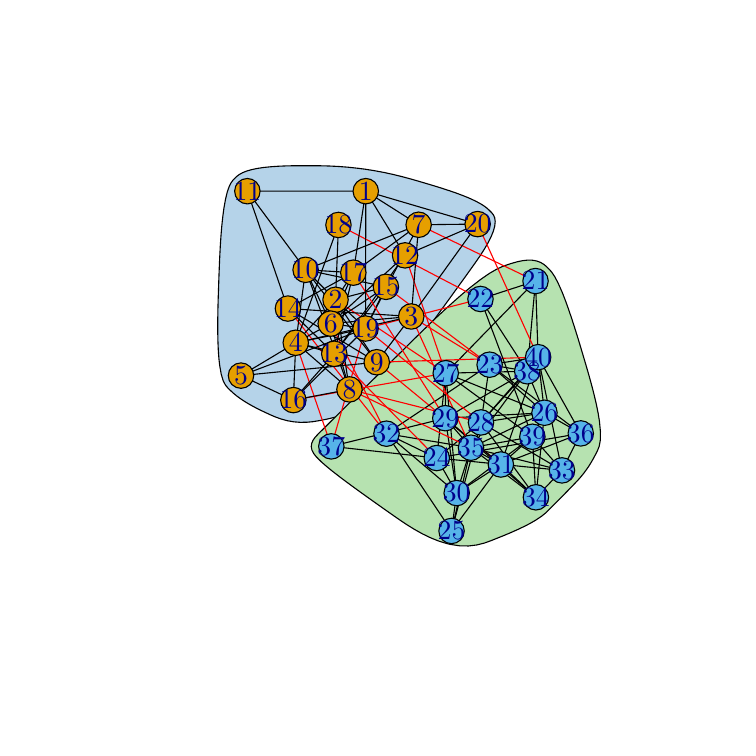
\begin{tikzpicture}[x=1pt,y=1pt]
\definecolor{fillColor}{RGB}{255,255,255}
\path[use as bounding box,fill=fillColor,fill opacity=0.00] (0,0) rectangle (252.94,252.94);
\begin{scope}
\path[clip] ( 49.20, 61.20) rectangle (227.75,203.75);
\definecolor{drawColor}{RGB}{0,0,0}
\definecolor{fillColor}{RGB}{181,211,233}

\path[draw=drawColor,line width= 0.4pt,line join=round,line cap=round,fill=fillColor] ( 96.15,110.51) --
	( 93.80,110.92) --
	( 91.54,111.54) --
	( 89.43,112.30) --
	( 87.48,113.14) --
	( 85.62,114.01) --
	( 83.72,114.92) --
	( 81.80,115.91) --
	( 79.91,116.95) --
	( 78.13,118.04) --
	( 78.12,118.04) --
	( 76.61,119.07) --
	( 75.27,120.07) --
	( 74.13,121.03) --
	( 73.17,121.93) --
	( 72.30,122.78) --
	( 71.46,123.79) --
	( 70.66,125.33) --
	( 69.94,127.69) --
	( 69.37,130.98) --
	( 69.10,133.35) --
	( 68.89,136.27) --
	( 68.75,139.53) --
	( 68.68,143.06) --
	( 68.68,146.80) --
	( 68.73,150.66) --
	( 68.83,154.59) --
	( 68.96,158.51) --
	( 69.09,162.44) --
	( 69.24,166.37) --
	( 69.41,170.29) --
	( 69.61,174.15) --
	( 69.86,177.90) --
	( 70.16,181.44) --
	( 70.51,184.70) --
	( 70.90,187.64) --
	( 70.91,187.71) --
	( 71.48,190.90) --
	( 72.10,193.46) --
	( 72.77,195.42) --
	( 73.46,196.82) --
	( 74.15,197.79) --
	( 74.84,198.51) --
	( 75.57,199.20) --
	( 76.47,199.88) --
	( 77.67,200.54) --
	( 79.21,201.15) --
	( 81.12,201.69) --
	( 82.97,202.07) --
	( 85.34,202.43) --
	( 87.97,202.69) --
	( 90.79,202.88) --
	( 93.74,203.00) --
	( 96.72,203.05) --
	( 99.71,203.06) --
	(102.69,203.06) --
	(105.76,203.03) --
	(108.97,202.95) --
	(112.33,202.78) --
	(115.82,202.51) --
	(119.37,202.13) --
	(121.92,201.80) --
	(125.47,201.23) --
	(128.95,200.58) --
	(132.32,199.84) --
	(135.52,199.05) --
	(138.54,198.23) --
	(141.42,197.40) --
	(144.24,196.57) --
	(147.08,195.72) --
	(149.90,194.84) --
	(152.67,193.93) --
	(155.31,193.01) --
	(157.75,192.08) --
	(159.27,191.46) --
	(161.55,190.42) --
	(163.42,189.44) --
	(164.90,188.52) --
	(166.01,187.68) --
	(166.86,186.90) --
	(167.61,186.15) --
	(168.28,185.30) --
	(168.76,184.23) --
	(168.94,182.87) --
	(168.76,181.18) --
	(168.26,179.38) --
	(167.43,177.33) --
	(166.29,175.09) --
	(164.89,172.70) --
	(163.29,170.23) --
	(161.58,167.75) --
	(159.82,165.29) --
	(158.05,162.82) --
	(156.24,160.31) --
	(154.40,157.77) --
	(152.57,155.23) --
	(150.78,152.76) --
	(149.07,150.42) --
	(149.04,150.38) --
	(147.07,147.68) --
	(145.31,145.30) --
	(143.79,143.26) --
	(142.50,141.53) --
	(141.33,139.98) --
	(140.16,138.44) --
	(138.94,136.85) --
	(137.67,135.24) --
	(136.40,133.68) --
	(135.70,132.83) --
	(134.20,131.09) --
	(132.83,129.59) --
	(131.62,128.33) --
	(130.53,127.23) --
	(129.42,126.12) --
	(128.20,124.91) --
	(126.89,123.59) --
	(126.07,122.78) --
	(124.72,121.43) --
	(123.41,120.12) --
	(122.18,118.90) --
	(121.03,117.75) --
	(119.82,116.61) --
	(118.35,115.46) --
	(116.56,114.35) --
	(115.16,113.66) --
	(113.24,112.88) --
	(111.20,112.23) --
	(109.12,111.70) --
	(107.08,111.27) --
	(105.07,110.89) --
	(102.98,110.55) --
	(100.75,110.35) --
	( 98.40,110.33) --
	cycle;
\definecolor{fillColor}{RGB}{182,226,176}

\path[draw=drawColor,line width= 0.4pt,line join=round,line cap=round,fill=fillColor] (151.77, 66.44) --
	(148.79, 67.33) --
	(145.74, 68.54) --
	(142.68, 70.01) --
	(139.65, 71.71) --
	(136.69, 73.55) --
	(133.82, 75.49) --
	(131.00, 77.46) --
	(128.19, 79.44) --
	(125.37, 81.44) --
	(122.57, 83.43) --
	(119.84, 85.39) --
	(117.26, 87.27) --
	(114.87, 89.03) --
	(113.37, 90.15) --
	(110.23, 92.58) --
	(107.89, 94.49) --
	(106.28, 95.90) --
	(105.17, 96.98) --
	(104.18, 98.00) --
	(103.32, 99.10) --
	(102.72,100.28) --
	(102.48,101.51) --
	(102.48,101.64) --
	(102.65,102.78) --
	(103.14,103.89) --
	(103.88,104.94) --
	(104.77,105.90) --
	(105.73,106.86) --
	(107.02,108.14) --
	(109.00,110.11) --
	(111.84,112.93) --
	(114.49,115.55) --
	(116.74,117.78) --
	(119.21,120.22) --
	(121.86,122.85) --
	(124.67,125.62) --
	(127.56,128.48) --
	(130.51,131.39) --
	(133.47,134.32) --
	(136.42,137.23) --
	(139.37,140.15) --
	(142.35,143.06) --
	(145.35,145.97) --
	(148.35,148.82) --
	(151.31,151.57) --
	(154.20,154.18) --
	(156.96,156.59) --
	(159.56,158.77) --
	(159.99,159.11) --
	(163.72,161.99) --
	(166.91,164.19) --
	(169.55,165.71) --
	(171.69,166.69) --
	(173.50,167.33) --
	(175.26,167.89) --
	(177.05,168.38) --
	(178.85,168.75) --
	(180.61,168.94) --
	(182.26,168.92) --
	(182.37,168.91) --
	(183.97,168.62) --
	(185.37,168.10) --
	(186.55,167.38) --
	(187.53,166.56) --
	(188.42,165.68) --
	(189.34,164.63) --
	(190.40,163.05) --
	(191.63,160.74) --
	(193.01,157.64) --
	(193.48,156.48) --
	(194.50,153.83) --
	(195.55,150.88) --
	(196.63,147.69) --
	(197.71,144.33) --
	(198.79,140.88) --
	(199.84,137.41) --
	(200.87,133.94) --
	(201.90,130.47) --
	(202.90,126.98) --
	(203.86,123.50) --
	(204.73,120.08) --
	(205.50,116.80) --
	(206.12,113.72) --
	(206.58,110.91) --
	(206.60,110.78) --
	(206.97,106.90) --
	(206.92,103.87) --
	(206.52,101.68) --
	(205.90,100.09) --
	(205.20, 98.72) --
	(204.44, 97.29) --
	(203.59, 95.81) --
	(202.65, 94.31) --
	(201.99, 93.35) --
	(200.79, 91.73) --
	(199.58, 90.26) --
	(198.41, 88.98) --
	(197.29, 87.82) --
	(196.14, 86.63) --
	(194.89, 85.34) --
	(193.56, 83.99) --
	(192.88, 83.29) --
	(191.60, 82.00) --
	(190.38, 80.76) --
	(189.24, 79.62) --
	(188.19, 78.57) --
	(187.08, 77.51) --
	(185.60, 76.32) --
	(183.59, 74.98) --
	(181.38, 73.71) --
	(179.34, 72.67) --
	(177.11, 71.61) --
	(174.74, 70.55) --
	(172.32, 69.53) --
	(169.90, 68.55) --
	(167.50, 67.59) --
	(165.02, 66.70) --
	(162.32, 66.02) --
	(159.34, 65.65) --
	(156.11, 65.71) --
	(152.66, 66.23) --
	cycle;

\path[draw=drawColor,line width= 0.4pt,line join=round,line cap=round] (183.33,132.42) --
	(183.29,132.37) --
	(183.09,132.11) --
	(182.84,131.79) --
	(182.64,131.53) --
	(182.48,131.33) --
	(182.32,131.12) --
	(182.12,130.86) --
	(181.87,130.54) --
	(181.68,130.29) --
	(181.63,130.23);

\path[draw=drawColor,line width= 0.4pt,line join=round,line cap=round] (166.12,151.03) --
	(166.26,150.82) --
	(166.98,149.69) --
	(168.22,147.78) --
	(169.50,145.81) --
	(170.57,144.15) --
	(171.46,142.78) --
	(172.06,141.84) --
	(172.89,140.57) --
	(173.81,139.14) --
	(174.95,137.39) --
	(176.25,135.37) --
	(177.40,133.60) --
	(177.95,132.74) --
	(178.01,132.65);

\path[draw=drawColor,line width= 0.4pt,line join=round,line cap=round] (197.61,110.35) --
	(197.49,110.57) --
	(196.84,111.73) --
	(195.72,113.73) --
	(194.56,115.81) --
	(193.57,117.57) --
	(192.76,119.02) --
	(192.16,120.10) --
	(191.41,121.43) --
	(190.57,122.93) --
	(189.55,124.76) --
	(188.36,126.88) --
	(187.31,128.77) --
	(186.77,129.73) --
	(186.70,129.85);

\path[draw=drawColor,line width= 0.4pt,line join=round,line cap=round] (175.28, 96.76) --
	(175.52, 96.85) --
	(176.77, 97.34) --
	(178.89, 98.16) --
	(181.07, 99.01) --
	(182.91, 99.73) --
	(184.42,100.32) --
	(185.43,100.71) --
	(186.83,101.26) --
	(188.42,101.87) --
	(190.36,102.63) --
	(192.59,103.50) --
	(194.54,104.26) --
	(195.48,104.62) --
	(195.57,104.66);

\path[draw=drawColor,line width= 0.4pt,line join=round,line cap=round] (164.73,101.97) --
	(165.03,102.02) --
	(166.42,102.27) --
	(168.25,102.60) --
	(169.77,102.87) --
	(170.99,103.09) --
	(171.28,103.14) --
	(172.46,103.35) --
	(173.88,103.60) --
	(175.68,103.93) --
	(177.28,104.21) --
	(177.83,104.31) --
	(177.84,104.31);

\path[draw=drawColor,line width= 0.4pt,line join=round,line cap=round] (162.92,104.87) --
	(163.07,105.06) --
	(163.84,106.11) --
	(165.23,107.99) --
	(166.75,110.07) --
	(168.08,111.88) --
	(169.18,113.37) --
	(170.15,114.69) --
	(170.35,114.97) --
	(171.31,116.27) --
	(172.37,117.72) --
	(173.65,119.45) --
	(175.15,121.49) --
	(176.61,123.47) --
	(177.54,124.74) --
	(177.78,125.07) --
	(177.78,125.07);

\path[draw=drawColor,line width= 0.4pt,line join=round,line cap=round] (183.38, 87.83) --
	(183.36, 88.14) --
	(183.28, 89.55) --
	(183.18, 91.36) --
	(183.09, 92.84) --
	(183.02, 94.02) --
	(183.01, 94.18) --
	(182.94, 95.35) --
	(182.86, 96.77) --
	(182.76, 98.56) --
	(182.67,100.09) --
	(182.64,100.53) --
	(182.64,100.53);

\path[draw=drawColor,line width= 0.4pt,line join=round,line cap=round] (179.99, 86.03) --
	(179.78, 86.19) --
	(178.70, 87.02) --
	(176.93, 88.37) --
	(175.16, 89.72) --
	(173.70, 90.84) --
	(172.49, 91.77) --
	(171.92, 92.20) --
	(170.76, 93.08) --
	(169.44, 94.09) --
	(167.82, 95.33) --
	(165.97, 96.74) --
	(164.47, 97.89) --
	(163.88, 98.34) --
	(163.86, 98.36);

\path[draw=drawColor,line width= 0.4pt,line join=round,line cap=round] (192.12, 97.47) --
	(192.07, 97.68) --
	(191.82, 98.88) --
	(191.33,101.22) --
	(190.72,104.09) --
	(190.14,106.84) --
	(189.65,109.20) --
	(189.22,111.20) --
	(188.84,113.02) --
	(188.76,113.42) --
	(188.38,115.21) --
	(187.97,117.16) --
	(187.49,119.42) --
	(186.93,122.09) --
	(186.32,124.98) --
	(185.79,127.51) --
	(185.48,128.99) --
	(185.40,129.36) --
	(185.40,129.36);

\path[draw=drawColor,line width= 0.4pt,line join=round,line cap=round] (190.03, 96.42) --
	(189.90, 96.56) --
	(189.37, 97.17) --
	(188.69, 97.93) --
	(188.16, 98.55) --
	(187.72, 99.04) --
	(187.28, 99.54) --
	(186.74,100.15) --
	(186.07,100.91) --
	(185.53,101.53) --
	(185.41,101.67);
\definecolor{drawColor}{RGB}{255,0,0}

\path[draw=drawColor,line width= 0.4pt,line join=round,line cap=round] (120.81,139.80) --
	(120.75,139.60) --
	(120.42,138.45) --
	(119.75,136.15) --
	(118.91,133.25) --
	(118.08,130.39) --
	(117.35,127.91) --
	(116.74,125.79) --
	(116.19,123.91) --
	(115.91,122.93) --
	(115.38,121.10) --
	(114.81,119.14) --
	(114.14,116.87) --
	(113.37,114.20) --
	(112.51,111.25) --
	(111.72,108.54) --
	(111.20,106.73) --
	(111.01,106.10) --
	(111.00,106.06);
\definecolor{drawColor}{RGB}{0,0,0}

\path[draw=drawColor,line width= 0.4pt,line join=round,line cap=round] (188.60, 94.08) --
	(188.36, 94.13) --
	(187.09, 94.45) --
	(184.83, 95.01) --
	(182.36, 95.63) --
	(180.21, 96.17) --
	(178.44, 96.61) --
	(176.87, 97.00) --
	(176.63, 97.06) --
	(175.08, 97.45) --
	(173.35, 97.88) --
	(171.26, 98.40) --
	(168.82, 99.01) --
	(166.48, 99.59) --
	(165.02, 99.95) --
	(164.67,100.04) --
	(164.66,100.04);

\path[draw=drawColor,line width= 0.4pt,line join=round,line cap=round] (189.86, 89.65) --
	(189.78, 89.57) --
	(189.43, 89.21) --
	(188.99, 88.76) --
	(188.64, 88.39) --
	(188.36, 88.10) --
	(188.07, 87.80) --
	(187.72, 87.44) --
	(187.28, 86.99) --
	(186.93, 86.63) --
	(186.85, 86.54);

\path[draw=drawColor,line width= 0.4pt,line join=round,line cap=round] (134.20,105.47) --
	(134.45,105.43) --
	(135.78,105.21) --
	(138.02,104.84) --
	(140.33,104.46) --
	(142.27,104.13) --
	(143.87,103.87) --
	(144.93,103.69) --
	(146.42,103.45) --
	(148.10,103.17) --
	(150.15,102.83) --
	(152.51,102.43) --
	(154.57,102.09) --
	(155.56,101.93) --
	(155.66,101.91);

\path[draw=drawColor,line width= 0.4pt,line join=round,line cap=round] (172.50, 99.44) --
	(172.57, 99.64) --
	(172.98,100.81) --
	(173.76,103.07) --
	(174.72,105.82) --
	(175.62,108.42) --
	(176.39,110.65) --
	(177.05,112.54) --
	(177.65,114.26) --
	(177.72,114.48) --
	(178.32,116.19) --
	(178.96,118.05) --
	(179.72,120.23) --
	(180.61,122.79) --
	(181.56,125.55) --
	(182.38,127.91) --
	(182.84,129.23) --
	(182.94,129.52) --
	(182.94,129.52);

\path[draw=drawColor,line width= 0.4pt,line join=round,line cap=round] (174.45, 98.13) --
	(174.57, 98.24) --
	(175.09, 98.70) --
	(175.74, 99.27) --
	(176.26, 99.73) --
	(176.68,100.11) --
	(177.11,100.48) --
	(177.63,100.94) --
	(178.28,101.51) --
	(178.80,101.97) --
	(178.92,102.08);
\definecolor{drawColor}{RGB}{255,0,0}

\path[draw=drawColor,line width= 0.4pt,line join=round,line cap=round] (129.70,129.12) --
	(129.84,129.01) --
	(130.67,128.32) --
	(132.47,126.84) --
	(135.01,124.74) --
	(137.82,122.43) --
	(140.48,120.24) --
	(142.83,118.30) --
	(144.88,116.61) --
	(146.71,115.11) --
	(148.44,113.68) --
	(148.57,113.57) --
	(150.30,112.15) --
	(152.12,110.65) --
	(154.14,108.98) --
	(156.47,107.06) --
	(159.11,104.88) --
	(161.91,102.57) --
	(164.49,100.45) --
	(166.36, 98.91) --
	(167.27, 98.16) --
	(167.44, 98.02) --
	(167.44, 98.02);
\definecolor{drawColor}{RGB}{0,0,0}

\path[draw=drawColor,line width= 0.4pt,line join=round,line cap=round] (166.98, 97.35) --
	(166.91, 97.39) --
	(166.58, 97.57) --
	(166.18, 97.79) --
	(165.86, 97.98) --
	(165.60, 98.12) --
	(165.33, 98.27) --
	(165.01, 98.45) --
	(164.61, 98.68) --
	(164.28, 98.86) --
	(164.21, 98.90);

\path[draw=drawColor,line width= 0.4pt,line join=round,line cap=round] (174.35, 91.94) --
	(174.51, 91.80) --
	(175.20, 91.15) --
	(176.07, 90.34) --
	(176.76, 89.69) --
	(177.32, 89.16) --
	(177.88, 88.64) --
	(178.58, 87.99) --
	(179.44, 87.18) --
	(180.13, 86.53) --
	(180.29, 86.38);

\path[draw=drawColor,line width= 0.4pt,line join=round,line cap=round] (158.72, 87.52) --
	(158.91, 87.66) --
	(159.96, 88.45) --
	(161.83, 89.84) --
	(163.88, 91.36) --
	(165.67, 92.70) --
	(167.15, 93.80) --
	(168.46, 94.77) --
	(168.70, 94.95) --
	(169.99, 95.91) --
	(171.42, 96.98) --
	(173.15, 98.26) --
	(175.17, 99.77) --
	(177.13,101.22) --
	(178.37,102.14) --
	(178.68,102.37) --
	(178.68,102.37);

\path[draw=drawColor,line width= 0.4pt,line join=round,line cap=round] (156.41, 89.16) --
	(156.47, 89.36) --
	(156.75, 90.25) --
	(157.10, 91.36) --
	(157.38, 92.24) --
	(157.61, 92.96) --
	(157.84, 93.68) --
	(158.12, 94.57) --
	(158.47, 95.68) --
	(158.75, 96.57) --
	(158.81, 96.77);

\path[draw=drawColor,line width= 0.4pt,line join=round,line cap=round] (151.51, 87.74) --
	(151.32, 87.90) --
	(150.31, 88.75) --
	(148.54, 90.25) --
	(146.63, 91.87) --
	(144.98, 93.26) --
	(143.62, 94.41) --
	(142.41, 95.44) --
	(142.34, 95.50) --
	(141.13, 96.52) --
	(139.79, 97.66) --
	(138.16, 99.04) --
	(136.25,100.65) --
	(134.46,102.17) --
	(133.39,103.07) --
	(133.18,103.25) --
	(133.18,103.25);

\path[draw=drawColor,line width= 0.4pt,line join=round,line cap=round] (158.89, 87.27) --
	(159.11, 87.41) --
	(160.07, 88.03) --
	(161.27, 88.81) --
	(162.23, 89.43) --
	(163.01, 89.93) --
	(163.79, 90.43) --
	(164.75, 91.05) --
	(165.95, 91.83) --
	(166.91, 92.45) --
	(167.13, 92.59);

\path[draw=drawColor,line width= 0.4pt,line join=round,line cap=round] (154.90,114.12) --
	(155.11,114.23) --
	(156.24,114.89) --
	(158.27,116.05) --
	(160.49,117.32) --
	(162.43,118.43) --
	(164.03,119.34) --
	(165.44,120.15) --
	(165.71,120.31) --
	(167.11,121.11) --
	(168.66,121.99) --
	(170.53,123.06) --
	(172.72,124.32) --
	(174.84,125.53) --
	(176.18,126.30) --
	(176.51,126.49) --
	(176.52,126.49);

\path[draw=drawColor,line width= 0.4pt,line join=round,line cap=round] (146.43,110.72) --
	(146.23,110.67) --
	(145.04,110.38) --
	(142.72,109.80) --
	(139.84,109.09) --
	(137.08,108.41) --
	(134.70,107.82) --
	(132.67,107.32) --
	(130.85,106.87) --
	(130.31,106.74) --
	(128.51,106.29) --
	(126.57,105.81) --
	(124.31,105.25) --
	(121.65,104.59) --
	(118.75,103.88) --
	(116.18,103.24) --
	(114.63,102.86) --
	(114.20,102.75) --
	(114.19,102.75);

\path[draw=drawColor,line width= 0.4pt,line join=round,line cap=round] (153.93,108.36) --
	(154.01,108.26) --
	(154.39,107.82) --
	(154.86,107.28) --
	(155.24,106.85) --
	(155.55,106.49) --
	(155.86,106.14) --
	(156.24,105.70) --
	(156.71,105.16) --
	(157.09,104.73) --
	(157.17,104.63);

\path[draw=drawColor,line width= 0.4pt,line join=round,line cap=round] (154.37,108.80) --
	(154.53,108.66) --
	(155.44,107.87) --
	(157.24,106.29) --
	(159.50,104.32) --
	(161.70,102.40) --
	(163.60,100.74) --
	(165.22, 99.33) --
	(166.67, 98.06) --
	(167.28, 97.53) --
	(168.69, 96.30) --
	(170.22, 94.96) --
	(171.99, 93.42) --
	(174.07, 91.60) --
	(176.35, 89.61) --
	(178.42, 87.80) --
	(179.75, 86.65) --
	(180.17, 86.28) --
	(180.18, 86.27);

\path[draw=drawColor,line width= 0.4pt,line join=round,line cap=round] (154.44,108.88) --
	(154.65,108.70) --
	(155.72,107.81) --
	(157.33,106.47) --
	(158.81,105.24) --
	(159.99,104.25) --
	(160.95,103.46) --
	(161.98,102.60) --
	(163.18,101.60) --
	(164.68,100.35) --
	(166.27, 99.02) --
	(167.28, 98.18) --
	(167.46, 98.04);

\path[draw=drawColor,line width= 0.4pt,line join=round,line cap=round] (151.59,107.28) --
	(151.64,107.01) --
	(151.84,105.64) --
	(152.17,103.52) --
	(152.47,101.50) --
	(152.72, 99.87) --
	(152.93, 98.49) --
	(152.96, 98.30) --
	(153.17, 96.93) --
	(153.41, 95.35) --
	(153.71, 93.38) --
	(154.04, 91.23) --
	(154.27, 89.71) --
	(154.33, 89.32) --
	(154.33, 89.32);

\path[draw=drawColor,line width= 0.4pt,line join=round,line cap=round] (166.83,113.75) --
	(167.00,113.94) --
	(167.88,114.95) --
	(169.38,116.66) --
	(170.95,118.45) --
	(172.26,119.95) --
	(173.35,121.19) --
	(174.12,122.08) --
	(175.13,123.22) --
	(176.25,124.51) --
	(177.63,126.08) --
	(179.22,127.90) --
	(180.63,129.51) --
	(181.34,130.31) --
	(181.42,130.41);

\path[draw=drawColor,line width= 0.4pt,line join=round,line cap=round] (166.89,113.70) --
	(167.08,113.92) --
	(168.02,114.96) --
	(169.38,116.46) --
	(170.59,117.80) --
	(171.55,118.86) --
	(172.16,119.53) --
	(173.02,120.49) --
	(174.04,121.62) --
	(175.33,123.04) --
	(176.64,124.49) --
	(177.35,125.28) --
	(177.43,125.37);

\path[draw=drawColor,line width= 0.4pt,line join=round,line cap=round] (166.52,106.57) --
	(166.67,106.38) --
	(167.45,105.32) --
	(168.82,103.44) --
	(170.31,101.41) --
	(171.61, 99.65) --
	(172.68, 98.19) --
	(173.62, 96.90) --
	(173.72, 96.76) --
	(174.67, 95.48) --
	(175.72, 94.05) --
	(176.98, 92.32) --
	(178.46, 90.30) --
	(179.88, 88.38) --
	(180.73, 87.21) --
	(180.93, 86.95) --
	(180.93, 86.95);

\path[draw=drawColor,line width= 0.4pt,line join=round,line cap=round] (167.76,107.94) --
	(167.97,107.82) --
	(169.10,107.15) --
	(171.10,105.96) --
	(173.30,104.66) --
	(175.21,103.53) --
	(176.80,102.59) --
	(178.19,101.77) --
	(178.43,101.62) --
	(179.82,100.81) --
	(181.35, 99.90) --
	(183.20, 98.80) --
	(185.37, 97.52) --
	(187.46, 96.28) --
	(188.78, 95.50) --
	(189.10, 95.31) --
	(189.10, 95.31);

\path[draw=drawColor,line width= 0.4pt,line join=round,line cap=round] (154.78,125.37) --
	(154.96,125.23) --
	(155.97,124.49) --
	(157.89,123.08) --
	(160.16,121.42) --
	(162.26,119.88) --
	(164.02,118.58) --
	(165.54,117.47) --
	(166.72,116.61) --
	(168.13,115.57) --
	(169.67,114.44) --
	(171.49,113.11) --
	(173.64,111.53) --
	(175.89,109.88) --
	(177.70,108.55) --
	(178.55,107.93) --
	(178.66,107.85);

\path[draw=drawColor,line width= 0.4pt,line join=round,line cap=round] (155.67,128.20) --
	(155.93,128.20) --
	(157.29,128.24) --
	(159.52,128.29) --
	(161.74,128.34) --
	(163.57,128.38) --
	(165.10,128.42) --
	(165.79,128.44) --
	(167.25,128.47) --
	(168.90,128.51) --
	(170.95,128.56) --
	(173.26,128.61) --
	(175.15,128.66) --
	(175.88,128.67) --
	(175.91,128.67);

\path[draw=drawColor,line width= 0.4pt,line join=round,line cap=round] (180.30,158.08) --
	(180.16,157.93) --
	(179.33,157.09) --
	(177.66,155.38) --
	(175.51,153.17) --
	(173.35,150.95) --
	(171.44,148.99) --
	(169.81,147.32) --
	(168.37,145.85) --
	(167.29,144.73) --
	(165.92,143.33) --
	(164.46,141.83) --
	(162.78,140.10) --
	(160.81,138.08) --
	(158.61,135.83) --
	(156.52,133.68) --
	(155.00,132.13) --
	(154.35,131.46) --
	(154.28,131.39);
\definecolor{drawColor}{RGB}{255,0,0}

\path[draw=drawColor,line width= 0.4pt,line join=round,line cap=round] (115.07,152.05) --
	(115.24,151.94) --
	(116.21,151.30) --
	(118.19,149.97) --
	(120.79,148.24) --
	(123.43,146.48) --
	(125.79,144.92) --
	(127.80,143.58) --
	(129.57,142.40) --
	(131.15,141.35) --
	(132.81,140.24) --
	(134.59,139.06) --
	(136.61,137.71) --
	(138.98,136.14) --
	(141.63,134.37) --
	(144.21,132.65) --
	(146.16,131.36) --
	(147.09,130.74) --
	(147.23,130.64);

\path[draw=drawColor,line width= 0.4pt,line join=round,line cap=round] (111.57,141.90) --
	(111.67,141.71) --
	(112.21,140.64) --
	(113.29,138.51) --
	(114.66,135.80) --
	(116.02,133.14) --
	(117.19,130.81) --
	(118.19,128.84) --
	(119.09,127.08) --
	(119.58,126.12) --
	(120.44,124.41) --
	(121.37,122.58) --
	(122.44,120.46) --
	(123.70,117.98) --
	(125.09,115.24) --
	(126.38,112.70) --
	(127.25,110.99) --
	(127.56,110.37) --
	(127.58,110.33);
\definecolor{drawColor}{RGB}{0,0,0}

\path[draw=drawColor,line width= 0.4pt,line join=round,line cap=round] (151.48,123.50) --
	(151.50,123.30) --
	(151.61,122.09) --
	(151.83,119.71) --
	(152.10,116.72) --
	(152.37,113.81) --
	(152.60,111.30) --
	(152.79,109.16) --
	(152.97,107.24) --
	(153.04,106.43) --
	(153.21,104.56) --
	(153.40,102.54) --
	(153.61,100.20) --
	(153.86, 97.45) --
	(154.14, 94.43) --
	(154.39, 91.69) --
	(154.55, 89.94) --
	(154.60, 89.37) --
	(154.60, 89.36);

\path[draw=drawColor,line width= 0.4pt,line join=round,line cap=round] (151.02,123.49) --
	(151.02,123.30) --
	(151.01,122.48) --
	(151.00,121.45) --
	(150.99,120.63) --
	(150.98,119.96) --
	(150.98,119.29) --
	(150.97,118.47) --
	(150.96,117.44) --
	(150.95,116.62) --
	(150.95,116.43);

\path[draw=drawColor,line width= 0.4pt,line join=round,line cap=round] (186.22,118.36) --
	(186.19,118.65) --
	(186.04,119.92) --
	(185.86,121.52) --
	(185.72,122.79) --
	(185.60,123.83) --
	(185.48,124.86) --
	(185.33,126.14) --
	(185.15,127.73) --
	(185.01,129.01) --
	(184.97,129.30);

\path[draw=drawColor,line width= 0.4pt,line join=round,line cap=round] (184.67,109.68) --
	(184.67,109.66) --
	(184.64,109.61) --
	(184.61,109.55) --
	(184.58,109.50) --
	(184.56,109.45) --
	(184.54,109.41) --
	(184.51,109.36) --
	(184.48,109.30) --
	(184.45,109.24) --
	(184.45,109.23);

\path[draw=drawColor,line width= 0.4pt,line join=round,line cap=round] (184.98,118.04) --
	(184.91,118.21) --
	(184.59,118.97) --
	(184.20,119.91) --
	(183.89,120.67) --
	(183.63,121.28) --
	(183.37,121.90) --
	(183.06,122.66) --
	(182.67,123.60) --
	(182.35,124.36) --
	(182.28,124.53);

\path[draw=drawColor,line width= 0.4pt,line join=round,line cap=round] (190.75,111.51) --
	(190.88,111.43) --
	(191.48,111.09) --
	(192.22,110.67) --
	(192.82,110.33) --
	(193.30,110.06) --
	(193.79,109.78) --
	(194.38,109.44) --
	(195.13,109.02) --
	(195.72,108.68) --
	(195.86,108.60);

\path[draw=drawColor,line width= 0.4pt,line join=round,line cap=round] (182.59,111.81) --
	(182.35,111.70) --
	(181.12,111.11) --
	(179.11,110.15) --
	(177.11,109.20) --
	(175.46,108.42) --
	(174.09,107.76) --
	(173.47,107.47) --
	(172.16,106.85) --
	(170.66,106.13) --
	(168.82,105.26) --
	(166.73,104.26) --
	(165.03,103.46) --
	(164.38,103.15) --
	(164.35,103.13);

\path[draw=drawColor,line width= 0.4pt,line join=round,line cap=round] (186.28,109.20) --
	(186.26,108.95) --
	(186.12,107.61) --
	(185.89,105.36) --
	(185.66,103.05) --
	(185.46,101.11) --
	(185.30, 99.52) --
	(185.20, 98.51) --
	(185.05, 97.02) --
	(184.88, 95.33) --
	(184.67, 93.27) --
	(184.43, 90.90) --
	(184.22, 88.85) --
	(184.12, 87.90) --
	(184.11, 87.82);

\path[draw=drawColor,line width= 0.4pt,line join=round,line cap=round] (182.15,113.53) --
	(181.92,113.52) --
	(180.63,113.45) --
	(178.28,113.32) --
	(175.61,113.18) --
	(173.24,113.05) --
	(171.27,112.94) --
	(169.55,112.85) --
	(168.82,112.81) --
	(167.16,112.72) --
	(165.33,112.62) --
	(163.14,112.50) --
	(160.56,112.36) --
	(157.97,112.21) --
	(156.14,112.11) --
	(155.52,112.08) --
	(155.50,112.08);

\path[draw=drawColor,line width= 0.4pt,line join=round,line cap=round] (182.20,113.09) --
	(181.90,113.05) --
	(180.51,112.83) --
	(178.61,112.55) --
	(177.01,112.30) --
	(175.74,112.11) --
	(175.27,112.04) --
	(174.06,111.85) --
	(172.61,111.63) --
	(170.78,111.35) --
	(169.06,111.09) --
	(168.37,110.98) --
	(168.35,110.98);

\path[draw=drawColor,line width= 0.4pt,line join=round,line cap=round] (182.47,115.50) --
	(182.26,115.58) --
	(181.09,116.05) --
	(178.89,116.94) --
	(176.29,117.98) --
	(173.90,118.94) --
	(171.89,119.74) --
	(170.18,120.43) --
	(168.91,120.94) --
	(167.29,121.59) --
	(165.52,122.29) --
	(163.44,123.13) --
	(160.98,124.12) --
	(158.40,125.15) --
	(156.37,125.96) --
	(155.45,126.33) --
	(155.34,126.38);

\path[draw=drawColor,line width= 0.4pt,line join=round,line cap=round] (154.21, 75.57) --
	(154.26, 75.81) --
	(154.57, 77.12) --
	(155.09, 79.33) --
	(155.62, 81.61) --
	(156.07, 83.51) --
	(156.44, 85.09) --
	(156.68, 86.12) --
	(157.02, 87.59) --
	(157.41, 89.24) --
	(157.88, 91.27) --
	(158.43, 93.60) --
	(158.90, 95.62) --
	(159.13, 96.58) --
	(159.15, 96.67);

\path[draw=drawColor,line width= 0.4pt,line join=round,line cap=round] (150.60, 74.91) --
	(150.48, 75.09) --
	(149.80, 76.10) --
	(148.47, 78.09) --
	(146.83, 80.55) --
	(145.25, 82.91) --
	(143.89, 84.94) --
	(142.74, 86.67) --
	(141.70, 88.22) --
	(141.41, 88.66) --
	(140.38, 90.19) --
	(139.27, 91.85) --
	(137.98, 93.79) --
	(136.46, 96.06) --
	(134.80, 98.54) --
	(133.34,100.73) --
	(132.46,102.04) --
	(132.22,102.40) --
	(132.22,102.40);

\path[draw=drawColor,line width= 0.4pt,line join=round,line cap=round] (155.90, 74.78) --
	(156.06, 74.99) --
	(156.87, 76.08) --
	(158.20, 77.87) --
	(159.55, 79.69) --
	(160.67, 81.19) --
	(161.59, 82.44) --
	(162.08, 83.09) --
	(162.95, 84.27) --
	(163.95, 85.61) --
	(165.18, 87.26) --
	(166.57, 89.14) --
	(167.74, 90.71) --
	(168.22, 91.36) --
	(168.25, 91.39);

\path[draw=drawColor,line width= 0.4pt,line join=round,line cap=round] (154.36, 75.53) --
	(154.42, 75.74) --
	(154.75, 76.93) --
	(155.37, 79.24) --
	(156.13, 82.03) --
	(156.84, 84.66) --
	(157.45, 86.90) --
	(157.97, 88.81) --
	(158.44, 90.56) --
	(158.48, 90.69) --
	(158.95, 92.43) --
	(159.46, 94.31) --
	(160.06, 96.52) --
	(160.77, 99.13) --
	(161.53,101.93) --
	(162.17,104.30) --
	(162.52,105.58) --
	(162.59,105.84) --
	(162.59,105.84);

\path[draw=drawColor,line width= 0.4pt,line join=round,line cap=round] (143.25, 97.94) --
	(143.03, 97.96) --
	(141.77, 98.10) --
	(139.41, 98.36) --
	(136.64, 98.67) --
	(134.09, 98.95) --
	(131.94, 99.19) --
	(130.11, 99.39) --
	(128.77, 99.54) --
	(127.05, 99.73) --
	(125.16, 99.94) --
	(122.93,100.18) --
	(120.30,100.47) --
	(117.54,100.78) --
	(115.38,101.02) --
	(114.40,101.12) --
	(114.30,101.14);

\path[draw=drawColor,line width= 0.4pt,line join=round,line cap=round] (152.37, 98.21) --
	(152.56, 98.24) --
	(153.66, 98.43) --
	(156.00, 98.83) --
	(159.17, 99.37) --
	(162.54, 99.95) --
	(165.64,100.48) --
	(168.32,100.94) --
	(170.66,101.33) --
	(172.79,101.70) --
	(173.85,101.88) --
	(175.93,102.24) --
	(178.14,102.61) --
	(180.63,103.04) --
	(183.52,103.53) --
	(186.79,104.09) --
	(190.14,104.67) --
	(192.98,105.15) --
	(194.72,105.45) --
	(195.30,105.55) --
	(195.32,105.55);

\path[draw=drawColor,line width= 0.4pt,line join=round,line cap=round] (152.41, 96.98) --
	(152.62, 96.96) --
	(153.80, 96.84) --
	(156.18, 96.61) --
	(159.22, 96.31) --
	(162.25, 96.01) --
	(164.90, 95.74) --
	(167.16, 95.52) --
	(169.16, 95.32) --
	(170.45, 95.20) --
	(172.37, 95.01) --
	(174.44, 94.80) --
	(176.81, 94.57) --
	(179.60, 94.29) --
	(182.69, 93.99) --
	(185.60, 93.70) --
	(187.62, 93.50) --
	(188.42, 93.42) --
	(188.48, 93.41);

\path[draw=drawColor,line width= 0.4pt,line join=round,line cap=round] (143.69, 99.44) --
	(143.43, 99.56) --
	(142.27,100.12) --
	(140.83,100.82) --
	(139.68,101.38) --
	(138.75,101.83) --
	(137.81,102.28) --
	(136.66,102.84) --
	(135.22,103.54) --
	(134.06,104.10) --
	(133.80,104.22);

\path[draw=drawColor,line width= 0.4pt,line join=round,line cap=round] (150.10, 93.43) --
	(150.17, 93.31) --
	(150.48, 92.76) --
	(150.87, 92.08) --
	(151.18, 91.54) --
	(151.43, 91.10) --
	(151.68, 90.66) --
	(151.98, 90.12) --
	(152.37, 89.44) --
	(152.68, 88.90) --
	(152.75, 88.77);

\path[draw=drawColor,line width= 0.4pt,line join=round,line cap=round] (151.42,100.32) --
	(151.65,100.51) --
	(152.68,101.33) --
	(153.96,102.36) --
	(154.98,103.19) --
	(155.81,103.86) --
	(156.65,104.53) --
	(157.67,105.36) --
	(158.95,106.39) --
	(159.98,107.21) --
	(160.21,107.40);

\path[draw=drawColor,line width= 0.4pt,line join=round,line cap=round] (148.31,102.01) --
	(148.34,102.26) --
	(148.48,103.60) --
	(148.72,105.86) --
	(148.96,108.18) --
	(149.17,110.12) --
	(149.34,111.72) --
	(149.45,112.76) --
	(149.61,114.26) --
	(149.78,115.94) --
	(150.00,118.01) --
	(150.25,120.39) --
	(150.47,122.45) --
	(150.57,123.42) --
	(150.58,123.51);

\path[draw=drawColor,line width= 0.4pt,line join=round,line cap=round] (171.47,131.86) --
	(171.70,131.90) --
	(172.68,132.05) --
	(173.91,132.24) --
	(174.89,132.39) --
	(175.69,132.52) --
	(176.49,132.64) --
	(177.47,132.79) --
	(178.69,132.98) --
	(179.68,133.13) --
	(179.90,133.17);

\path[draw=drawColor,line width= 0.4pt,line join=round,line cap=round] (171.46,130.37) --
	(171.58,130.35) --
	(172.10,130.25) --
	(172.76,130.14) --
	(173.29,130.05) --
	(173.72,129.97) --
	(174.15,129.90) --
	(174.67,129.80) --
	(175.33,129.69) --
	(175.86,129.60) --
	(175.98,129.58);
\definecolor{drawColor}{RGB}{255,0,0}

\path[draw=drawColor,line width= 0.4pt,line join=round,line cap=round] (133.13,156.52) --
	(133.29,156.40) --
	(134.24,155.69) --
	(136.15,154.26) --
	(138.62,152.40) --
	(141.12,150.53) --
	(143.33,148.87) --
	(145.21,147.46) --
	(146.87,146.21) --
	(148.19,145.22) --
	(149.76,144.04) --
	(151.45,142.78) --
	(153.38,141.33) --
	(155.64,139.63) --
	(158.16,137.74) --
	(160.59,135.92) --
	(162.36,134.59) --
	(163.14,134.00) --
	(163.24,133.92);
\definecolor{drawColor}{RGB}{0,0,0}

\path[draw=drawColor,line width= 0.4pt,line join=round,line cap=round] (170.60,128.39) --
	(170.77,128.26) --
	(171.76,127.52) --
	(173.67,126.08) --
	(175.99,124.32) --
	(178.21,122.65) --
	(180.10,121.23) --
	(181.71,120.02) --
	(183.17,118.91) --
	(183.39,118.74) --
	(184.85,117.65) --
	(186.42,116.46) --
	(188.26,115.07) --
	(190.43,113.44) --
	(192.77,111.68) --
	(194.78,110.16) --
	(195.92,109.30) --
	(196.18,109.10) --
	(196.18,109.10);

\path[draw=drawColor,line width= 0.4pt,line join=round,line cap=round] (163.10,128.60) --
	(162.92,128.49) --
	(161.93,127.82) --
	(159.94,126.49) --
	(157.41,124.80) --
	(154.92,123.13) --
	(152.74,121.67) --
	(150.89,120.43) --
	(149.24,119.33) --
	(148.29,118.69) --
	(146.70,117.63) --
	(144.99,116.48) --
	(143.01,115.16) --
	(140.69,113.61) --
	(138.13,111.90) --
	(135.75,110.30) --
	(134.13,109.22) --
	(133.53,108.82) --
	(133.49,108.79);

\path[draw=drawColor,line width= 0.4pt,line join=round,line cap=round] (153.78, 75.65) --
	(153.80, 75.77) --
	(153.87, 76.30) --
	(153.96, 76.96) --
	(154.03, 77.49) --
	(154.09, 77.93) --
	(154.15, 78.36) --
	(154.22, 78.89) --
	(154.31, 79.56) --
	(154.38, 80.09) --
	(154.40, 80.21);

\path[draw=drawColor,line width= 0.4pt,line join=round,line cap=round] (166.24,126.61) --
	(166.19,126.30) --
	(165.99,124.92) --
	(165.73,123.21) --
	(165.53,121.84) --
	(165.36,120.72) --
	(165.19,119.61) --
	(164.99,118.24) --
	(164.73,116.52) --
	(164.53,115.15) --
	(164.48,114.84);

\path[draw=drawColor,line width= 0.4pt,line join=round,line cap=round] (170.39,128.13) --
	(170.59,127.94) --
	(171.64,127.03) --
	(173.22,125.64) --
	(174.69,124.36) --
	(175.86,123.33) --
	(176.83,122.47) --
	(177.85,121.59) --
	(179.03,120.55) --
	(180.50,119.26) --
	(182.08,117.88) --
	(183.09,116.99) --
	(183.28,116.82);
\definecolor{drawColor}{RGB}{255,0,0}

\path[draw=drawColor,line width= 0.4pt,line join=round,line cap=round] (130.75,132.20) --
	(130.92,132.20) --
	(132.01,132.23) --
	(134.34,132.31) --
	(137.63,132.41) --
	(141.27,132.52) --
	(144.73,132.63) --
	(147.79,132.73) --
	(150.45,132.81) --
	(152.83,132.88) --
	(155.08,132.95) --
	(155.30,132.96) --
	(157.54,133.03) --
	(159.90,133.10) --
	(162.53,133.19) --
	(165.54,133.28) --
	(168.97,133.39) --
	(172.61,133.50) --
	(175.97,133.61) --
	(178.41,133.68) --
	(179.61,133.72) --
	(179.85,133.73) --
	(179.85,133.73);
\definecolor{drawColor}{RGB}{0,0,0}

\path[draw=drawColor,line width= 0.4pt,line join=round,line cap=round] (165.24,150.59) --
	(165.31,150.41) --
	(165.70,149.36) --
	(166.54,147.15) --
	(167.67,144.13) --
	(168.89,140.92) --
	(170.00,137.95) --
	(170.97,135.38) --
	(171.81,133.14) --
	(172.58,131.11) --
	(172.99,130.01) --
	(173.74,128.02) --
	(174.54,125.91) --
	(175.43,123.54) --
	(176.47,120.79) --
	(177.64,117.69) --
	(178.84,114.49) --
	(179.87,111.75) --
	(180.52,110.05) --
	(180.74,109.46) --
	(180.75,109.43);
\definecolor{drawColor}{RGB}{255,0,0}

\path[draw=drawColor,line width= 0.4pt,line join=round,line cap=round] (120.73,121.11) --
	(120.93,121.06) --
	(122.05,120.77) --
	(124.36,120.19) --
	(127.41,119.43) --
	(130.55,118.64) --
	(133.37,117.93) --
	(135.78,117.33) --
	(137.89,116.79) --
	(139.86,116.30) --
	(140.03,116.26) --
	(142.00,115.76) --
	(144.09,115.24) --
	(146.47,114.64) --
	(149.25,113.94) --
	(152.37,113.16) --
	(155.46,112.38) --
	(157.86,111.78) --
	(159.09,111.47) --
	(159.33,111.41) --
	(159.33,111.41);

\path[draw=drawColor,line width= 0.4pt,line join=round,line cap=round] (116.39,179.53) --
	(116.55,179.44) --
	(117.51,178.94) --
	(119.58,177.86) --
	(122.50,176.34) --
	(125.71,174.66) --
	(128.76,173.08) --
	(131.45,171.67) --
	(133.78,170.45) --
	(135.88,169.36) --
	(137.86,168.33) --
	(137.96,168.28) --
	(139.94,167.24) --
	(142.03,166.16) --
	(144.35,164.95) --
	(147.02,163.55) --
	(150.05,161.97) --
	(153.26,160.30) --
	(156.21,158.76) --
	(158.33,157.65) --
	(159.35,157.12) --
	(159.53,157.03) --
	(159.53,157.03);
\definecolor{drawColor}{RGB}{0,0,0}

\path[draw=drawColor,line width= 0.4pt,line join=round,line cap=round] (183.67,156.78) --
	(183.68,156.50) --
	(183.73,155.12) --
	(183.80,152.97) --
	(183.87,150.91) --
	(183.93,149.26) --
	(183.97,147.85) --
	(183.98,147.62) --
	(184.03,146.23) --
	(184.08,144.63) --
	(184.15,142.64) --
	(184.23,140.45) --
	(184.28,138.89) --
	(184.29,138.47) --
	(184.29,138.47);

\path[draw=drawColor,line width= 0.4pt,line join=round,line cap=round] (183.09,156.79) --
	(183.07,156.55) --
	(182.95,155.23) --
	(182.73,152.93) --
	(182.51,150.47) --
	(182.31,148.36) --
	(182.15,146.62) --
	(182.01,145.08) --
	(181.87,143.52) --
	(181.71,141.78) --
	(181.51,139.66) --
	(181.29,137.20) --
	(181.08,134.91) --
	(180.96,133.60) --
	(180.93,133.37);
\definecolor{drawColor}{RGB}{255,0,0}

\path[draw=drawColor,line width= 0.4pt,line join=round,line cap=round] ( 98.37,134.73) --
	( 98.44,134.52) --
	( 98.85,133.34) --
	( 99.62,131.08) --
	(100.54,128.39) --
	(101.41,125.87) --
	(102.13,123.75) --
	(102.76,121.94) --
	(103.30,120.36) --
	(103.87,118.68) --
	(104.50,116.86) --
	(105.24,114.71) --
	(106.10,112.18) --
	(107.03,109.49) --
	(107.78,107.28) --
	(108.16,106.17) --
	(108.23,106.00);
\definecolor{drawColor}{RGB}{0,0,0}

\path[draw=drawColor,line width= 0.4pt,line join=round,line cap=round] (195.15, 97.07) --
	(195.22, 97.20) --
	(195.53, 97.80) --
	(195.91, 98.56) --
	(196.22, 99.16) --
	(196.46, 99.64) --
	(196.71,100.13) --
	(197.02,100.73) --
	(197.40,101.49) --
	(197.71,102.09) --
	(197.77,102.22);
\definecolor{drawColor}{RGB}{255,0,0}

\path[draw=drawColor,line width= 0.4pt,line join=round,line cap=round] (145.43,179.72) --
	(145.61,179.63) --
	(146.67,179.12) --
	(148.83,178.08) --
	(151.62,176.74) --
	(154.43,175.39) --
	(156.92,174.19) --
	(159.04,173.17) --
	(160.91,172.27) --
	(162.40,171.55) --
	(164.17,170.69) --
	(166.07,169.78) --
	(168.25,168.73) --
	(170.80,167.50) --
	(173.64,166.13) --
	(176.37,164.82) --
	(178.37,163.86) --
	(179.25,163.43) --
	(179.36,163.38);

\path[draw=drawColor,line width= 0.4pt,line join=round,line cap=round] (142.52,146.17) --
	(142.73,146.04) --
	(143.85,145.35) --
	(145.83,144.13) --
	(147.96,142.82) --
	(149.80,141.69) --
	(151.32,140.76) --
	(152.68,139.92) --
	(152.76,139.87) --
	(154.11,139.04) --
	(155.61,138.12) --
	(157.43,137.00) --
	(159.55,135.69) --
	(161.56,134.46) --
	(162.75,133.73) --
	(163.00,133.57) --
	(163.00,133.57);
\definecolor{drawColor}{RGB}{0,0,0}

\path[draw=drawColor,line width= 0.4pt,line join=round,line cap=round] (179.13,159.95) --
	(178.84,159.86) --
	(177.54,159.43) --
	(175.92,158.90) --
	(174.62,158.48) --
	(173.56,158.14) --
	(172.51,157.79) --
	(171.21,157.37) --
	(169.59,156.84) --
	(168.29,156.42) --
	(167.99,156.32);
\definecolor{drawColor}{RGB}{255,0,0}

\path[draw=drawColor,line width= 0.4pt,line join=round,line cap=round] (126.56,145.37) --
	(126.76,145.42) --
	(127.94,145.72) --
	(130.26,146.32) --
	(133.14,147.06) --
	(135.93,147.78) --
	(138.33,148.40) --
	(140.38,148.92) --
	(142.22,149.40) --
	(142.86,149.56) --
	(144.66,150.03) --
	(146.61,150.53) --
	(148.87,151.11) --
	(151.54,151.79) --
	(154.45,152.54) --
	(157.05,153.21) --
	(158.67,153.63) --
	(159.15,153.75) --
	(159.16,153.75);

\path[draw=drawColor,line width= 0.4pt,line join=round,line cap=round] (164.51,177.77) --
	(164.58,177.60) --
	(165.05,176.57) --
	(166.03,174.42) --
	(167.36,171.48) --
	(168.77,168.37) --
	(170.08,165.51) --
	(171.20,163.03) --
	(172.18,160.87) --
	(173.08,158.90) --
	(173.53,157.92) --
	(174.40,155.99) --
	(175.33,153.95) --
	(176.37,151.65) --
	(177.59,148.98) --
	(178.96,145.96) --
	(180.36,142.86) --
	(181.56,140.24) --
	(182.29,138.62) --
	(182.53,138.09) --
	(182.55,138.06);
\definecolor{drawColor}{RGB}{0,0,0}

\path[draw=drawColor,line width= 0.4pt,line join=round,line cap=round] ( 99.27,121.60) --
	( 99.43,121.76) --
	(100.34,122.67) --
	(102.02,124.33) --
	(103.95,126.24) --
	(105.69,127.96) --
	(107.13,129.39) --
	(108.38,130.63) --
	(109.05,131.29) --
	(110.25,132.48) --
	(111.57,133.79) --
	(113.14,135.35) --
	(114.99,137.18) --
	(116.88,139.05) --
	(118.27,140.43) --
	(118.80,140.95) --
	(118.83,140.98);
\definecolor{drawColor}{RGB}{255,0,0}

\path[draw=drawColor,line width= 0.4pt,line join=round,line cap=round] (100.53,119.16) --
	(100.72,119.19) --
	(101.80,119.39) --
	(104.11,119.79) --
	(107.33,120.36) --
	(110.82,120.98) --
	(114.10,121.56) --
	(116.97,122.07) --
	(119.47,122.51) --
	(121.71,122.90) --
	(123.53,123.23) --
	(125.69,123.61) --
	(127.96,124.01) --
	(130.51,124.46) --
	(133.44,124.98) --
	(136.78,125.56) --
	(140.27,126.18) --
	(143.38,126.73) --
	(145.51,127.11) --
	(146.42,127.27) --
	(146.53,127.29);
\definecolor{drawColor}{RGB}{0,0,0}

\path[draw=drawColor,line width= 0.4pt,line join=round,line cap=round] (127.43,155.15) --
	(127.34,154.97) --
	(126.96,154.18) --
	(126.47,153.19) --
	(126.09,152.40) --
	(125.77,151.75) --
	(125.46,151.11) --
	(125.07,150.32) --
	(124.59,149.33) --
	(124.20,148.54) --
	(124.12,148.36);
\definecolor{drawColor}{RGB}{255,0,0}

\path[draw=drawColor,line width= 0.4pt,line join=round,line cap=round] ( 96.89,147.83) --
	( 97.00,147.68) --
	( 97.67,146.83) --
	( 99.12,144.99) --
	(101.15,142.41) --
	(103.39,139.58) --
	(105.50,136.89) --
	(107.37,134.52) --
	(108.99,132.46) --
	(110.44,130.62) --
	(111.82,128.87) --
	(111.85,128.84) --
	(113.23,127.09) --
	(114.68,125.24) --
	(116.30,123.19) --
	(118.16,120.83) --
	(120.27,118.15) --
	(122.50,115.31) --
	(124.55,112.72) --
	(126.01,110.87) --
	(126.69,109.99) --
	(126.81,109.85) --
	(126.81,109.85);
\definecolor{drawColor}{RGB}{0,0,0}

\path[draw=drawColor,line width= 0.4pt,line join=round,line cap=round] (101.39,140.00) --
	(101.66,140.06) --
	(103.03,140.34) --
	(105.06,140.75) --
	(106.91,141.13) --
	(108.38,141.43) --
	(109.49,141.65) --
	(110.78,141.92) --
	(112.30,142.23) --
	(114.20,142.61) --
	(116.20,143.02) --
	(117.41,143.27) --
	(117.59,143.30);

\path[draw=drawColor,line width= 0.4pt,line join=round,line cap=round] ( 98.07,153.66) --
	( 98.31,153.79) --
	( 99.53,154.46) --
	(101.40,155.48) --
	(103.16,156.45) --
	(104.57,157.22) --
	(105.77,157.88) --
	(105.85,157.93) --
	(107.06,158.58) --
	(108.44,159.35) --
	(110.18,160.30) --
	(112.06,161.33) --
	(113.34,162.03) --
	(113.64,162.19) --
	(113.64,162.19);

\path[draw=drawColor,line width= 0.4pt,line join=round,line cap=round] (111.84,139.58) --
	(111.89,139.83) --
	(112.20,141.14) --
	(112.72,143.33) --
	(113.24,145.55) --
	(113.67,147.39) --
	(114.03,148.91) --
	(114.23,149.75) --
	(114.57,151.19) --
	(114.95,152.82) --
	(115.42,154.83) --
	(115.96,157.12) --
	(116.41,159.05) --
	(116.61,159.87) --
	(116.62,159.92);

\path[draw=drawColor,line width= 0.4pt,line join=round,line cap=round] (107.73,131.64) --
	(107.53,131.41) --
	(106.60,130.36) --
	(105.37,128.97) --
	(104.36,127.83) --
	(103.56,126.92) --
	(103.39,126.73) --
	(102.60,125.84) --
	(101.65,124.76) --
	(100.45,123.40) --
	( 99.39,122.20) --
	( 99.05,121.81) --
	( 99.05,121.81);

\path[draw=drawColor,line width= 0.4pt,line join=round,line cap=round] (113.59,138.74) --
	(113.75,138.94) --
	(114.57,140.01) --
	(115.95,141.80) --
	(117.37,143.63) --
	(118.55,145.16) --
	(119.52,146.42) --
	(120.12,147.19) --
	(121.03,148.37) --
	(122.06,149.71) --
	(123.33,151.35) --
	(124.78,153.23) --
	(126.02,154.85) --
	(126.59,155.58) --
	(126.64,155.64);

\path[draw=drawColor,line width= 0.4pt,line join=round,line cap=round] (107.49,138.31) --
	(107.27,138.52) --
	(106.27,139.50) --
	(104.89,140.85) --
	(103.71,142.00) --
	(102.78,142.91) --
	(102.41,143.27) --
	(101.53,144.13) --
	(100.47,145.16) --
	( 99.14,146.46) --
	( 97.88,147.69) --
	( 97.35,148.21) --
	( 97.33,148.23);

\path[draw=drawColor,line width= 0.4pt,line join=round,line cap=round] (140.59,172.48) --
	(140.84,172.58) --
	(142.10,173.12) --
	(144.11,173.99) --
	(146.09,174.84) --
	(147.70,175.54) --
	(149.05,176.12) --
	(149.48,176.31) --
	(150.79,176.87) --
	(152.29,177.52) --
	(154.15,178.32) --
	(156.23,179.21) --
	(157.83,179.90) --
	(158.36,180.13) --
	(158.37,180.14);

\path[draw=drawColor,line width= 0.4pt,line join=round,line cap=round] (133.68,166.92) --
	(133.55,166.75) --
	(132.85,165.77) --
	(131.45,163.83) --
	(129.70,161.38) --
	(127.98,159.00) --
	(126.49,156.93) --
	(125.22,155.17) --
	(124.09,153.60) --
	(123.57,152.87) --
	(122.47,151.34) --
	(121.28,149.69) --
	(119.91,147.78) --
	(118.29,145.53) --
	(116.51,143.06) --
	(114.89,140.80) --
	(113.83,139.34) --
	(113.48,138.85) --
	(113.47,138.83);

\path[draw=drawColor,line width= 0.4pt,line join=round,line cap=round] ( 80.89,189.50) --
	( 80.95,189.30) --
	( 81.34,188.17) --
	( 82.13,185.91) --
	( 83.12,183.03) --
	( 84.10,180.19) --
	( 84.96,177.71) --
	( 85.69,175.61) --
	( 86.33,173.73) --
	( 86.71,172.65) --
	( 87.34,170.83) --
	( 88.01,168.88) --
	( 88.79,166.64) --
	( 89.70,164.00) --
	( 90.70,161.09) --
	( 91.64,158.37) --
	( 92.28,156.53) --
	( 92.52,155.84) --
	( 92.53,155.80);

\path[draw=drawColor,line width= 0.4pt,line join=round,line cap=round] (105.02,165.17) --
	(105.23,165.15) --
	(106.17,165.10) --
	(107.34,165.03) --
	(108.28,164.97) --
	(109.05,164.93) --
	(109.81,164.88) --
	(110.75,164.82) --
	(111.92,164.75) --
	(112.86,164.70) --
	(113.08,164.68);

\path[draw=drawColor,line width= 0.4pt,line join=round,line cap=round] (104.92,164.49) --
	(105.18,164.43) --
	(106.51,164.15) --
	(108.69,163.69) --
	(110.89,163.22) --
	(112.70,162.84) --
	(114.20,162.52) --
	(114.93,162.36) --
	(116.37,162.06) --
	(118.00,161.72) --
	(120.00,161.29) --
	(122.28,160.81) --
	(124.15,160.41) --
	(124.91,160.25) --
	(124.95,160.24);

\path[draw=drawColor,line width= 0.4pt,line join=round,line cap=round] ( 97.68,169.14) --
	( 97.54,169.33) --
	( 96.77,170.37) --
	( 95.37,172.26) --
	( 93.80,174.38) --
	( 92.41,176.26) --
	( 91.26,177.81) --
	( 90.26,179.17) --
	( 89.90,179.65) --
	( 88.92,180.97) --
	( 87.84,182.43) --
	( 86.54,184.19) --
	( 85.01,186.25) --
	( 83.49,188.30) --
	( 82.46,189.70) --
	( 82.13,190.14) --
	( 82.12,190.15);

\path[draw=drawColor,line width= 0.4pt,line join=round,line cap=round] (122.20,134.43) --
	(122.01,134.55) --
	(120.92,135.21) --
	(118.89,136.43) --
	(116.53,137.86) --
	(114.39,139.15) --
	(112.60,140.23) --
	(111.06,141.16) --
	(110.09,141.75) --
	(108.62,142.63) --
	(107.02,143.60) --
	(105.11,144.76) --
	(102.86,146.11) --
	(100.54,147.52) --
	( 98.77,148.58) --
	( 98.04,149.03) --
	( 97.98,149.06);

\path[draw=drawColor,line width= 0.4pt,line join=round,line cap=round] (111.75,121.36) --
	(111.45,121.31) --
	(110.14,121.06) --
	(108.51,120.75) --
	(107.20,120.50) --
	(106.14,120.29) --
	(105.07,120.09) --
	(103.76,119.84) --
	(102.13,119.53) --
	(100.82,119.28) --
	(100.52,119.22);
\definecolor{drawColor}{RGB}{255,0,0}

\path[draw=drawColor,line width= 0.4pt,line join=round,line cap=round] (137.87,166.30) --
	(137.94,166.11) --
	(138.33,164.98) --
	(139.11,162.72) --
	(140.10,159.84) --
	(141.08,156.99) --
	(141.95,154.50) --
	(142.68,152.38) --
	(143.33,150.50) --
	(143.72,149.37) --
	(144.34,147.55) --
	(145.02,145.60) --
	(145.79,143.36) --
	(146.71,140.71) --
	(147.71,137.79) --
	(148.66,135.06) --
	(149.30,133.20) --
	(149.55,132.49) --
	(149.56,132.44);
\definecolor{drawColor}{RGB}{0,0,0}

\path[draw=drawColor,line width= 0.4pt,line join=round,line cap=round] (114.68,126.55) --
	(114.61,126.74) --
	(114.21,127.85) --
	(113.38,130.10) --
	(112.32,132.99) --
	(111.27,135.87) --
	(110.33,138.41) --
	(109.54,140.57) --
	(108.84,142.48) --
	(108.34,143.84) --
	(107.67,145.66) --
	(106.95,147.63) --
	(106.13,149.88) --
	(105.16,152.52) --
	(104.08,155.45) --
	(103.06,158.24) --
	(102.34,160.22) --
	(102.03,161.04) --
	(102.01,161.12);

\path[draw=drawColor,line width= 0.4pt,line join=round,line cap=round] (139.19,177.62) --
	(139.09,177.43) --
	(138.53,176.34) --
	(137.44,174.21) --
	(136.10,171.58) --
	(134.81,169.06) --
	(133.70,166.90) --
	(132.76,165.06) --
	(131.91,163.40) --
	(131.69,162.97) --
	(130.85,161.33) --
	(129.94,159.55) --
	(128.88,157.49) --
	(127.64,155.05) --
	(126.29,152.41) --
	(125.09,150.08) --
	(124.38,148.69) --
	(124.20,148.33) --
	(124.20,148.32);

\path[draw=drawColor,line width= 0.4pt,line join=round,line cap=round] (137.57,179.00) --
	(137.36,178.84) --
	(136.26,178.03) --
	(134.47,176.72) --
	(132.69,175.41) --
	(131.22,174.34) --
	(130.00,173.45) --
	(129.48,173.06) --
	(128.31,172.20) --
	(126.97,171.23) --
	(125.33,170.02) --
	(123.47,168.66) --
	(121.97,167.56) --
	(121.41,167.15) --
	(121.39,167.13);

\path[draw=drawColor,line width= 0.4pt,line join=round,line cap=round] (137.00,180.01) --
	(136.81,179.94) --
	(135.69,179.49) --
	(133.47,178.61) --
	(130.67,177.49) --
	(127.93,176.40) --
	(125.55,175.45) --
	(123.52,174.65) --
	(121.72,173.93) --
	(120.85,173.58) --
	(119.09,172.88) --
	(117.20,172.12) --
	(115.01,171.25) --
	(112.43,170.23) --
	(109.60,169.10) --
	(107.00,168.06) --
	(105.30,167.39) --
	(104.72,167.16) --
	(104.70,167.15);

\path[draw=drawColor,line width= 0.4pt,line join=round,line cap=round] (141.29,152.32) --
	(141.41,152.49) --
	(142.13,153.50) --
	(143.53,155.44) --
	(145.23,157.80) --
	(146.84,160.04) --
	(148.22,161.96) --
	(149.39,163.59) --
	(150.46,165.07) --
	(150.60,165.27) --
	(151.66,166.75) --
	(152.81,168.34) --
	(154.15,170.21) --
	(155.74,172.42) --
	(157.44,174.79) --
	(158.91,176.83) --
	(159.73,177.97) --
	(159.91,178.22) --
	(159.91,178.22);

\path[draw=drawColor,line width= 0.4pt,line join=round,line cap=round] (114.05,145.36) --
	(114.14,145.35) --
	(114.55,145.29) --
	(115.06,145.22) --
	(115.46,145.16) --
	(115.79,145.11) --
	(116.13,145.07) --
	(116.53,145.01) --
	(117.04,144.94) --
	(117.45,144.88) --
	(117.54,144.87);

\path[draw=drawColor,line width= 0.4pt,line join=round,line cap=round] (111.36,150.21) --
	(111.48,150.47) --
	(112.00,151.64) --
	(112.64,153.09) --
	(113.16,154.26) --
	(113.58,155.20) --
	(114.00,156.15) --
	(114.52,157.32) --
	(115.17,158.77) --
	(115.68,159.94) --
	(115.80,160.20);

\path[draw=drawColor,line width= 0.4pt,line join=round,line cap=round] (113.32,148.55) --
	(113.57,148.72) --
	(114.74,149.50) --
	(116.38,150.59) --
	(117.80,151.53) --
	(118.92,152.28) --
	(119.47,152.64) --
	(120.52,153.34) --
	(121.76,154.17) --
	(123.32,155.21) --
	(124.86,156.23) --
	(125.57,156.71) --
	(125.62,156.74);

\path[draw=drawColor,line width= 0.4pt,line join=round,line cap=round] (112.88,149.11) --
	(113.05,149.27) --
	(114.00,150.14) --
	(115.74,151.74) --
	(117.73,153.56) --
	(119.51,155.20) --
	(121.00,156.56) --
	(122.29,157.74) --
	(122.93,158.33) --
	(124.17,159.47) --
	(125.53,160.72) --
	(127.16,162.21) --
	(129.07,163.96) --
	(131.02,165.75) --
	(132.43,167.04) --
	(132.95,167.52) --
	(132.97,167.54);

\path[draw=drawColor,line width= 0.4pt,line join=round,line cap=round] (107.54,150.17) --
	(107.41,150.46) --
	(106.82,151.74) --
	(106.07,153.34) --
	(105.46,154.63) --
	(104.98,155.68) --
	(104.96,155.72) --
	(104.47,156.76) --
	(103.87,158.04) --
	(103.13,159.64) --
	(102.52,160.95) --
	(102.37,161.27) --
	(102.37,161.27);

\path[draw=drawColor,line width= 0.4pt,line join=round,line cap=round] (110.75,141.57) --
	(110.83,141.30) --
	(111.22,139.95) --
	(111.77,138.01) --
	(112.26,136.29) --
	(112.65,134.94) --
	(112.88,134.11) --
	(113.23,132.88) --
	(113.65,131.42) --
	(114.17,129.59) --
	(114.70,127.73) --
	(114.98,126.75) --
	(115.01,126.65);

\path[draw=drawColor,line width= 0.4pt,line join=round,line cap=round] ( 81.25,125.26) --
	( 81.53,125.13) --
	( 82.77,124.55) --
	( 84.31,123.83) --
	( 85.54,123.26) --
	( 86.54,122.79) --
	( 87.54,122.32) --
	( 88.78,121.74) --
	( 90.32,121.02) --
	( 91.55,120.44) --
	( 91.83,120.31);

\path[draw=drawColor,line width= 0.4pt,line join=round,line cap=round] ( 81.39,128.84) --
	( 81.58,128.91) --
	( 82.67,129.32) --
	( 84.90,130.17) --
	( 87.83,131.27) --
	( 90.81,132.40) --
	( 93.47,133.40) --
	( 95.75,134.26) --
	( 97.74,135.02) --
	( 99.59,135.72) --
	(101.46,136.43) --
	(103.46,137.18) --
	(105.74,138.04) --
	(108.41,139.05) --
	(111.40,140.18) --
	(114.32,141.28) --
	(116.54,142.12) --
	(117.61,142.53) --
	(117.79,142.60);

\path[draw=drawColor,line width= 0.4pt,line join=round,line cap=round] ( 81.67,127.66) --
	( 81.86,127.68) --
	( 83.01,127.80) --
	( 85.38,128.03) --
	( 88.52,128.34) --
	( 91.76,128.66) --
	( 94.66,128.95) --
	( 97.16,129.19) --
	( 99.34,129.41) --
	(101.37,129.61) --
	(101.61,129.63) --
	(103.64,129.83) --
	(105.79,130.04) --
	(108.24,130.29) --
	(111.10,130.57) --
	(114.30,130.88) --
	(117.49,131.20) --
	(119.99,131.44) --
	(121.29,131.57) --
	(121.56,131.60) --
	(121.56,131.60);
\definecolor{drawColor}{RGB}{255,0,0}

\path[draw=drawColor,line width= 0.4pt,line join=round,line cap=round] (125.67,141.32) --
	(125.81,141.20) --
	(126.68,140.49) --
	(128.51,139.00) --
	(131.02,136.96) --
	(133.71,134.78) --
	(136.19,132.75) --
	(138.35,131.00) --
	(140.23,129.47) --
	(141.93,128.08) --
	(142.95,127.25) --
	(144.61,125.90) --
	(146.36,124.48) --
	(148.34,122.87) --
	(150.62,121.01) --
	(153.21,118.90) --
	(155.88,116.73) --
	(158.19,114.85) --
	(159.66,113.65) --
	(160.19,113.22) --
	(160.23,113.19);
\definecolor{drawColor}{RGB}{0,0,0}

\path[draw=drawColor,line width= 0.4pt,line join=round,line cap=round] ( 98.44,143.41) --
	( 98.51,143.61) --
	( 98.92,144.73) --
	( 99.74,146.98) --
	(100.78,149.85) --
	(101.81,152.69) --
	(102.71,155.19) --
	(103.48,157.31) --
	(104.16,159.19) --
	(104.59,160.37) --
	(105.25,162.18) --
	(105.95,164.13) --
	(106.76,166.37) --
	(107.72,169.00) --
	(108.77,171.91) --
	(109.76,174.65) --
	(110.45,176.54) --
	(110.71,177.27) --
	(110.74,177.33);

\path[draw=drawColor,line width= 0.4pt,line join=round,line cap=round] ( 96.68,134.48) --
	( 96.67,134.18) --
	( 96.61,132.83) --
	( 96.54,131.16) --
	( 96.48,129.81) --
	( 96.44,128.72) --
	( 96.39,127.63) --
	( 96.34,126.29) --
	( 96.26,124.61) --
	( 96.21,123.26) --
	( 96.19,122.96);

\path[draw=drawColor,line width= 0.4pt,line join=round,line cap=round] (101.30,137.81) --
	(101.43,137.78) --
	(102.02,137.61) --
	(102.76,137.39) --
	(103.35,137.23) --
	(103.83,137.09) --
	(104.31,136.95) --
	(104.90,136.78) --
	(105.63,136.57) --
	(106.22,136.40) --
	(106.36,136.36);
\definecolor{drawColor}{RGB}{255,0,0}

\path[draw=drawColor,line width= 0.4pt,line join=round,line cap=round] (120.13,160.51) --
	(120.22,160.37) --
	(120.79,159.48) --
	(122.02,157.53) --
	(123.80,154.71) --
	(125.81,151.53) --
	(127.77,148.43) --
	(129.52,145.65) --
	(131.06,143.23) --
	(132.42,141.07) --
	(133.68,139.07) --
	(134.29,138.12) --
	(135.53,136.15) --
	(136.84,134.08) --
	(138.28,131.80) --
	(139.92,129.20) --
	(141.79,126.25) --
	(143.80,123.06) --
	(145.74,120.00) --
	(147.27,117.58) --
	(148.15,116.18) --
	(148.43,115.74) --
	(148.44,115.72);
\definecolor{drawColor}{RGB}{0,0,0}

\path[draw=drawColor,line width= 0.4pt,line join=round,line cap=round] ( 97.49,143.65) --
	( 97.53,143.92) --
	( 97.71,145.30) --
	( 97.99,147.39) --
	( 98.25,149.35) --
	( 98.47,150.91) --
	( 98.65,152.25) --
	( 98.65,152.26) --
	( 98.83,153.61) --
	( 99.04,155.17) --
	( 99.30,157.12) --
	( 99.58,159.21) --
	( 99.77,160.60) --
	( 99.81,160.88) --
	( 99.81,160.88);

\path[draw=drawColor,line width= 0.4pt,line join=round,line cap=round] (101.35,138.01) --
	(101.60,137.95) --
	(102.92,137.63) --
	(105.10,137.11) --
	(107.32,136.57) --
	(109.15,136.13) --
	(110.68,135.77) --
	(111.51,135.57) --
	(112.95,135.22) --
	(114.58,134.83) --
	(116.58,134.35) --
	(118.87,133.80) --
	(120.79,133.34) --
	(121.61,133.14) --
	(121.67,133.13);

\path[draw=drawColor,line width= 0.4pt,line join=round,line cap=round] (100.35,136.06) --
	(100.56,135.88) --
	(101.62,134.96) --
	(103.18,133.60) --
	(104.60,132.37) --
	(105.73,131.39) --
	(106.57,130.66) --
	(107.57,129.79) --
	(108.74,128.77) --
	(110.20,127.50) --
	(111.74,126.17) --
	(112.66,125.37) --
	(112.79,125.25);

\path[draw=drawColor,line width= 0.4pt,line join=round,line cap=round] (100.91,141.30) --
	(101.03,141.36) --
	(101.56,141.65) --
	(102.22,142.02) --
	(102.75,142.31) --
	(103.18,142.54) --
	(103.61,142.78) --
	(104.14,143.07) --
	(104.80,143.43) --
	(105.33,143.72) --
	(105.45,143.79);

\path[draw=drawColor,line width= 0.4pt,line join=round,line cap=round] ( 92.93,136.72) --
	( 92.67,136.56) --
	( 91.46,135.84) --
	( 89.83,134.86) --
	( 88.45,134.03) --
	( 87.35,133.37) --
	( 86.98,133.15) --
	( 85.93,132.52) --
	( 84.68,131.77) --
	( 83.10,130.82) --
	( 81.62,129.94) --
	( 81.05,129.59) --
	( 81.03,129.58);

\path[draw=drawColor,line width= 0.4pt,line join=round,line cap=round] (145.89,181.77) --
	(146.20,181.77) --
	(147.61,181.79) --
	(149.37,181.81) --
	(150.78,181.83) --
	(151.93,181.84) --
	(151.94,181.84) --
	(153.09,181.85) --
	(154.49,181.87) --
	(156.25,181.89) --
	(157.67,181.90) --
	(158.00,181.91) --
	(158.00,181.91);

\path[draw=drawColor,line width= 0.4pt,line join=round,line cap=round] (134.00,148.87) --
	(133.80,148.89) --
	(132.60,148.96) --
	(130.21,149.12) --
	(127.19,149.31) --
	(124.20,149.50) --
	(121.60,149.67) --
	(119.38,149.81) --
	(117.41,149.94) --
	(116.32,150.01) --
	(114.41,150.13) --
	(112.36,150.27) --
	(109.99,150.42) --
	(107.21,150.60) --
	(104.14,150.79) --
	(101.29,150.98) --
	( 99.37,151.10) --
	( 98.67,151.15) --
	( 98.63,151.15);
\definecolor{drawColor}{RGB}{255,0,0}

\path[draw=drawColor,line width= 0.4pt,line join=round,line cap=round] (140.51,144.39) --
	(140.59,144.22) --
	(141.06,143.19) --
	(142.04,141.03) --
	(143.37,138.11) --
	(144.77,135.03) --
	(146.06,132.20) --
	(147.17,129.76) --
	(148.14,127.64) --
	(149.02,125.70) --
	(149.40,124.87) --
	(150.27,122.96) --
	(151.19,120.93) --
	(152.23,118.64) --
	(153.44,115.99) --
	(154.81,112.98) --
	(156.20,109.92) --
	(157.37,107.36) --
	(158.07,105.83) --
	(158.28,105.36) --
	(158.29,105.35);
\definecolor{drawColor}{RGB}{0,0,0}

\path[draw=drawColor,line width= 0.4pt,line join=round,line cap=round] (135.83,144.90) --
	(135.65,144.66) --
	(134.84,143.59) --
	(133.83,142.25) --
	(133.03,141.18) --
	(132.37,140.32) --
	(131.72,139.45) --
	(130.91,138.38) --
	(129.90,137.04) --
	(129.10,135.97) --
	(128.91,135.73);

\path[draw=drawColor,line width= 0.4pt,line join=round,line cap=round] (138.97,153.17) --
	(138.99,153.41) --
	(139.10,154.73) --
	(139.28,157.04) --
	(139.49,159.53) --
	(139.66,161.69) --
	(139.80,163.47) --
	(139.93,165.05) --
	(139.94,165.15) --
	(140.07,166.73) --
	(140.21,168.49) --
	(140.38,170.61) --
	(140.58,173.10) --
	(140.77,175.45) --
	(140.89,176.84) --
	(140.91,177.13) --
	(140.91,177.13);

\path[draw=drawColor,line width= 0.4pt,line join=round,line cap=round] (134.01,148.17) --
	(133.75,148.15) --
	(132.39,148.03) --
	(130.18,147.83) --
	(127.99,147.64) --
	(126.18,147.48) --
	(124.68,147.35) --
	(124.05,147.29) --
	(122.60,147.16) --
	(120.96,147.02) --
	(118.93,146.84) --
	(116.63,146.63) --
	(114.79,146.47) --
	(114.10,146.41) --
	(114.08,146.41);

\path[draw=drawColor,line width= 0.4pt,line join=round,line cap=round] (134.11,147.56) --
	(133.90,147.51) --
	(132.72,147.24) --
	(130.38,146.71) --
	(127.48,146.05) --
	(124.68,145.41) --
	(122.26,144.86) --
	(120.21,144.39) --
	(118.37,143.97) --
	(117.74,143.83) --
	(115.92,143.42) --
	(113.96,142.97) --
	(111.68,142.45) --
	(109.00,141.84) --
	(106.08,141.18) --
	(103.46,140.58) --
	(101.85,140.21) --
	(101.37,140.11) --
	(101.36,140.11);

\path[draw=drawColor,line width= 0.4pt,line join=round,line cap=round] (114.56,151.42) --
	(114.68,151.32) --
	(115.17,150.85) --
	(115.78,150.26) --
	(116.27,149.80) --
	(116.67,149.41) --
	(117.07,149.03) --
	(117.56,148.56) --
	(118.17,147.98) --
	(118.66,147.51) --
	(118.77,147.40);

\path[draw=drawColor,line width= 0.4pt,line join=round,line cap=round] (111.42,159.21) --
	(111.43,159.48) --
	(111.48,160.86) --
	(111.57,163.00) --
	(111.65,165.01) --
	(111.71,166.63) --
	(111.77,168.01) --
	(111.77,168.13) --
	(111.82,169.50) --
	(111.89,171.09) --
	(111.97,173.07) --
	(112.05,175.22) --
	(112.11,176.71) --
	(112.12,177.05) --
	(112.12,177.05);

\path[draw=drawColor,line width= 0.4pt,line join=round,line cap=round] (113.76,158.45) --
	(113.80,158.51) --
	(113.96,158.76) --
	(114.16,159.06) --
	(114.32,159.31) --
	(114.45,159.51) --
	(114.59,159.71) --
	(114.75,159.95) --
	(114.95,160.26) --
	(115.11,160.50) --
	(115.14,160.56);

\path[draw=drawColor,line width= 0.4pt,line join=round,line cap=round] (115.70,155.75) --
	(115.94,155.81) --
	(117.03,156.09) --
	(118.38,156.44) --
	(119.46,156.72) --
	(120.34,156.95) --
	(121.22,157.17) --
	(122.31,157.45) --
	(123.66,157.80) --
	(124.74,158.08) --
	(124.99,158.14);
\definecolor{drawColor}{RGB}{255,0,0}

\path[draw=drawColor,line width= 0.4pt,line join=round,line cap=round] (114.01,131.81) --
	(114.14,131.68) --
	(114.93,130.87) --
	(116.59,129.19) --
	(118.85,126.89) --
	(121.25,124.45) --
	(123.45,122.21) --
	(125.37,120.27) --
	(127.03,118.58) --
	(128.55,117.04) --
	(129.31,116.26) --
	(130.79,114.75) --
	(132.36,113.15) --
	(134.14,111.35) --
	(136.19,109.26) --
	(138.52,106.90) --
	(140.90,104.47) --
	(142.93,102.42) --
	(144.17,101.15) --
	(144.58,100.73) --
	(144.60,100.71);
\definecolor{drawColor}{RGB}{0,0,0}

\path[draw=drawColor,line width= 0.4pt,line join=round,line cap=round] (107.98,157.86) --
	(107.87,157.98) --
	(107.37,158.48) --
	(106.74,159.11) --
	(106.24,159.62) --
	(105.83,160.02) --
	(105.42,160.43) --
	(104.92,160.94) --
	(104.29,161.57) --
	(103.79,162.07) --
	(103.67,162.18);

\path[draw=drawColor,line width= 0.4pt,line join=round,line cap=round] (113.77,150.77) --
	(113.93,150.54) --
	(114.69,149.38) --
	(115.87,147.60) --
	(116.98,145.92) --
	(117.87,144.57) --
	(118.63,143.42) --
	(118.69,143.33) --
	(119.45,142.18) --
	(120.32,140.86) --
	(121.41,139.21) --
	(122.60,137.41) --
	(123.42,136.18) --
	(123.60,135.89) --
	(123.60,135.89);

\path[draw=drawColor,line width= 0.4pt,line join=round,line cap=round] (111.94,150.06) --
	(111.98,149.81) --
	(112.18,148.50) --
	(112.54,146.22) --
	(112.92,143.78) --
	(113.25,141.68) --
	(113.51,139.95) --
	(113.75,138.42) --
	(113.99,136.87) --
	(114.26,135.14) --
	(114.59,133.04) --
	(114.97,130.59) --
	(115.32,128.32) --
	(115.53,127.01) --
	(115.56,126.78);

\path[draw=drawColor,line width= 0.4pt,line join=round,line cap=round] (108.11,151.23) --
	(107.90,151.00) --
	(106.95,149.97) --
	(105.77,148.70) --
	(104.82,147.68) --
	(104.06,146.84) --
	(103.29,146.01) --
	(102.34,144.99) --
	(101.16,143.72) --
	(100.22,142.69) --
	(100.00,142.46);

\path[draw=drawColor,line width= 0.4pt,line join=round,line cap=round] (126.59,192.56) --
	(126.79,192.50) --
	(127.97,192.16) --
	(130.26,191.48) --
	(133.09,190.65) --
	(135.81,189.85) --
	(138.14,189.16) --
	(140.12,188.58) --
	(141.91,188.05) --
	(142.39,187.91) --
	(144.16,187.39) --
	(146.07,186.83) --
	(148.30,186.17) --
	(150.92,185.40) --
	(153.77,184.56) --
	(156.28,183.82) --
	(157.78,183.38) --
	(158.18,183.26) --
	(158.18,183.26);

\path[draw=drawColor,line width= 0.4pt,line join=round,line cap=round] (122.16,189.26) --
	(122.16,189.06) --
	(122.16,187.91) --
	(122.16,185.53) --
	(122.15,182.37) --
	(122.15,179.10) --
	(122.14,176.15) --
	(122.14,173.63) --
	(122.14,171.42) --
	(122.13,169.37) --
	(122.13,169.04) --
	(122.13,167.00) --
	(122.13,164.83) --
	(122.12,162.36) --
	(122.12,159.49) --
	(122.12,156.25) --
	(122.11,153.03) --
	(122.11,150.48) --
	(122.10,149.13) --
	(122.10,148.83) --
	(122.10,148.83);

\path[draw=drawColor,line width= 0.4pt,line join=round,line cap=round] (121.47,189.31) --
	(121.44,189.05) --
	(121.23,187.71) --
	(120.89,185.50) --
	(120.55,183.27) --
	(120.27,181.43) --
	(120.04,179.90) --
	(119.92,179.13) --
	(119.70,177.68) --
	(119.45,176.03) --
	(119.14,174.00) --
	(118.78,171.69) --
	(118.49,169.78) --
	(118.37,169.00) --
	(118.37,168.96);

\path[draw=drawColor,line width= 0.4pt,line join=round,line cap=round] (124.57,189.93) --
	(124.71,189.70) --
	(125.44,188.52) --
	(126.55,186.69) --
	(127.61,184.96) --
	(128.46,183.57) --
	(129.19,182.39) --
	(129.27,182.26) --
	(129.99,181.08) --
	(130.82,179.72) --
	(131.85,178.03) --
	(132.98,176.18) --
	(133.77,174.90) --
	(133.96,174.58) --
	(133.96,174.58);

\path[draw=drawColor,line width= 0.4pt,line join=round,line cap=round] (117.57,193.86) --
	(117.35,193.86) --
	(116.14,193.86) --
	(113.74,193.86) --
	(110.77,193.86) --
	(107.89,193.86) --
	(105.42,193.86) --
	(103.31,193.86) --
	(101.42,193.85) --
	(100.78,193.85) --
	( 98.91,193.85) --
	( 96.90,193.85) --
	( 94.57,193.85) --
	( 91.82,193.85) --
	( 88.82,193.85) --
	( 86.14,193.85) --
	( 84.48,193.85) --
	( 84.00,193.85) --
	( 83.99,193.85);

\path[draw=drawColor,line width= 0.4pt,line join=round,line cap=round] (123.33,135.70) --
	(123.20,135.87) --
	(122.46,136.84) --
	(121.00,138.73) --
	(119.20,141.07) --
	(117.47,143.32) --
	(115.98,145.24) --
	(114.72,146.88) --
	(113.58,148.36) --
	(113.28,148.75) --
	(112.16,150.21) --
	(110.94,151.79) --
	(109.52,153.63) --
	(107.85,155.80) --
	(106.04,158.15) --
	(104.44,160.23) --
	(103.49,161.46) --
	(103.23,161.79) --
	(103.23,161.80);
\definecolor{drawColor}{RGB}{255,0,0}

\path[draw=drawColor,line width= 0.4pt,line join=round,line cap=round] (120.42,120.24) --
	(120.60,120.15) --
	(121.65,119.65) --
	(123.80,118.62) --
	(126.63,117.26) --
	(129.53,115.87) --
	(132.13,114.62) --
	(134.36,113.55) --
	(136.31,112.61) --
	(138.13,111.74) --
	(138.23,111.69) --
	(140.05,110.82) --
	(141.99,109.89) --
	(144.20,108.83) --
	(146.78,107.59) --
	(149.67,106.20) --
	(152.53,104.84) --
	(154.73,103.78) --
	(155.84,103.25) --
	(156.05,103.15) --
	(156.05,103.15);
\definecolor{drawColor}{RGB}{0,0,0}

\path[draw=drawColor,line width= 0.4pt,line join=round,line cap=round] (126.06,191.39) --
	(126.31,191.23) --
	(127.50,190.47) --
	(129.08,189.47) --
	(130.40,188.63) --
	(131.45,187.97) --
	(131.73,187.79) --
	(132.74,187.15) --
	(133.96,186.37) --
	(135.50,185.39) --
	(136.90,184.50) --
	(137.39,184.19) --
	(137.40,184.19);
\definecolor{fillColor}{RGB}{230,159,0}

\path[draw=drawColor,line width= 0.4pt,line join=round,line cap=round,fill=fillColor] (122.17,193.86) circle (  4.60);

\path[draw=drawColor,line width= 0.4pt,line join=round,line cap=round,fill=fillColor] (111.24,154.61) circle (  4.60);

\path[draw=drawColor,line width= 0.4pt,line join=round,line cap=round,fill=fillColor] (138.60,148.58) circle (  4.60);

\path[draw=drawColor,line width= 0.4pt,line join=round,line cap=round,fill=fillColor] ( 96.87,139.08) circle (  4.60);

\path[draw=drawColor,line width= 0.4pt,line join=round,line cap=round,fill=fillColor] ( 77.08,127.21) circle (  4.60);

\path[draw=drawColor,line width= 0.4pt,line join=round,line cap=round,fill=fillColor] (109.49,146.00) circle (  4.60);

\path[draw=drawColor,line width= 0.4pt,line join=round,line cap=round,fill=fillColor] (141.28,181.72) circle (  4.60);

\path[draw=drawColor,line width= 0.4pt,line join=round,line cap=round,fill=fillColor] (116.27,122.23) circle (  4.60);

\path[draw=drawColor,line width= 0.4pt,line join=round,line cap=round,fill=fillColor] (126.14,132.05) circle (  4.60);

\path[draw=drawColor,line width= 0.4pt,line join=round,line cap=round,fill=fillColor] (100.42,165.44) circle (  4.60);

\path[draw=drawColor,line width= 0.4pt,line join=round,line cap=round,fill=fillColor] ( 79.38,193.85) circle (  4.60);

\path[draw=drawColor,line width= 0.4pt,line join=round,line cap=round,fill=fillColor] (136.37,170.66) circle (  4.60);

\path[draw=drawColor,line width= 0.4pt,line join=round,line cap=round,fill=fillColor] (110.78,135.09) circle (  4.60);

\path[draw=drawColor,line width= 0.4pt,line join=round,line cap=round,fill=fillColor] ( 94.04,151.44) circle (  4.60);

\path[draw=drawColor,line width= 0.4pt,line join=round,line cap=round,fill=fillColor] (129.45,159.29) circle (  4.60);

\path[draw=drawColor,line width= 0.4pt,line join=round,line cap=round,fill=fillColor] ( 96.00,118.36) circle (  4.60);

\path[draw=drawColor,line width= 0.4pt,line join=round,line cap=round,fill=fillColor] (117.67,164.41) circle (  4.60);

\path[draw=drawColor,line width= 0.4pt,line join=round,line cap=round,fill=fillColor] (112.30,181.65) circle (  4.60);

\path[draw=drawColor,line width= 0.4pt,line join=round,line cap=round,fill=fillColor] (122.10,144.22) circle (  4.60);

\path[draw=drawColor,line width= 0.4pt,line join=round,line cap=round,fill=fillColor] (162.60,181.96) circle (  4.60);
\definecolor{fillColor}{RGB}{86,180,233}

\path[draw=drawColor,line width= 0.4pt,line join=round,line cap=round,fill=fillColor] (183.51,161.38) circle (  4.60);

\path[draw=drawColor,line width= 0.4pt,line join=round,line cap=round,fill=fillColor] (163.62,154.90) circle (  4.60);

\path[draw=drawColor,line width= 0.4pt,line join=round,line cap=round,fill=fillColor] (166.92,131.16) circle (  4.60);

\path[draw=drawColor,line width= 0.4pt,line join=round,line cap=round,fill=fillColor] (147.83, 97.43) circle (  4.60);

\path[draw=drawColor,line width= 0.4pt,line join=round,line cap=round,fill=fillColor] (153.16, 71.08) circle (  4.60);

\path[draw=drawColor,line width= 0.4pt,line join=round,line cap=round,fill=fillColor] (186.75,113.79) circle (  4.60);

\path[draw=drawColor,line width= 0.4pt,line join=round,line cap=round,fill=fillColor] (151.07,128.09) circle (  4.60);

\path[draw=drawColor,line width= 0.4pt,line join=round,line cap=round,fill=fillColor] (163.80,110.29) circle (  4.60);

\path[draw=drawColor,line width= 0.4pt,line join=round,line cap=round,fill=fillColor] (150.90,111.83) circle (  4.60);

\path[draw=drawColor,line width= 0.4pt,line join=round,line cap=round,fill=fillColor] (155.02, 84.77) circle (  4.60);

\path[draw=drawColor,line width= 0.4pt,line join=round,line cap=round,fill=fillColor] (170.99, 95.09) circle (  4.60);

\path[draw=drawColor,line width= 0.4pt,line join=round,line cap=round,fill=fillColor] (129.66,106.23) circle (  4.60);

\path[draw=drawColor,line width= 0.4pt,line join=round,line cap=round,fill=fillColor] (193.07, 92.96) circle (  4.60);

\path[draw=drawColor,line width= 0.4pt,line join=round,line cap=round,fill=fillColor] (183.65, 83.24) circle (  4.60);

\path[draw=drawColor,line width= 0.4pt,line join=round,line cap=round,fill=fillColor] (160.20,101.16) circle (  4.60);

\path[draw=drawColor,line width= 0.4pt,line join=round,line cap=round,fill=fillColor] (199.86,106.33) circle (  4.60);

\path[draw=drawColor,line width= 0.4pt,line join=round,line cap=round,fill=fillColor] (109.72,101.64) circle (  4.60);

\path[draw=drawColor,line width= 0.4pt,line join=round,line cap=round,fill=fillColor] (180.51,128.78) circle (  4.60);

\path[draw=drawColor,line width= 0.4pt,line join=round,line cap=round,fill=fillColor] (182.37,105.12) circle (  4.60);

\path[draw=drawColor,line width= 0.4pt,line join=round,line cap=round,fill=fillColor] (184.45,133.87) circle (  4.60);
\end{scope}
\begin{scope}
\path[clip] (  0.00,  0.00) rectangle (252.94,252.94);
\definecolor{drawColor}{RGB}{0,0,139}

\node[text=drawColor,anchor=base,inner sep=0pt, outer sep=0pt, scale=  1.00] at (122.17,190.65) {1};

\node[text=drawColor,anchor=base,inner sep=0pt, outer sep=0pt, scale=  1.00] at (111.24,151.40) {2};

\node[text=drawColor,anchor=base,inner sep=0pt, outer sep=0pt, scale=  1.00] at (138.60,145.37) {3};

\node[text=drawColor,anchor=base,inner sep=0pt, outer sep=0pt, scale=  1.00] at ( 96.87,135.88) {4};

\node[text=drawColor,anchor=base,inner sep=0pt, outer sep=0pt, scale=  1.00] at ( 77.08,124.00) {5};

\node[text=drawColor,anchor=base,inner sep=0pt, outer sep=0pt, scale=  1.00] at (109.49,142.79) {6};

\node[text=drawColor,anchor=base,inner sep=0pt, outer sep=0pt, scale=  1.00] at (141.28,178.51) {7};

\node[text=drawColor,anchor=base,inner sep=0pt, outer sep=0pt, scale=  1.00] at (116.27,119.02) {8};

\node[text=drawColor,anchor=base,inner sep=0pt, outer sep=0pt, scale=  1.00] at (126.14,128.84) {9};

\node[text=drawColor,anchor=base,inner sep=0pt, outer sep=0pt, scale=  1.00] at (100.42,162.24) {10};

\node[text=drawColor,anchor=base,inner sep=0pt, outer sep=0pt, scale=  1.00] at ( 79.38,190.64) {11};

\node[text=drawColor,anchor=base,inner sep=0pt, outer sep=0pt, scale=  1.00] at (136.37,167.45) {12};

\node[text=drawColor,anchor=base,inner sep=0pt, outer sep=0pt, scale=  1.00] at (110.78,131.89) {13};

\node[text=drawColor,anchor=base,inner sep=0pt, outer sep=0pt, scale=  1.00] at ( 94.04,148.24) {14};

\node[text=drawColor,anchor=base,inner sep=0pt, outer sep=0pt, scale=  1.00] at (129.45,156.08) {15};

\node[text=drawColor,anchor=base,inner sep=0pt, outer sep=0pt, scale=  1.00] at ( 96.00,115.15) {16};

\node[text=drawColor,anchor=base,inner sep=0pt, outer sep=0pt, scale=  1.00] at (117.67,161.20) {17};

\node[text=drawColor,anchor=base,inner sep=0pt, outer sep=0pt, scale=  1.00] at (112.30,178.45) {18};

\node[text=drawColor,anchor=base,inner sep=0pt, outer sep=0pt, scale=  1.00] at (122.10,141.02) {19};

\node[text=drawColor,anchor=base,inner sep=0pt, outer sep=0pt, scale=  1.00] at (162.60,178.75) {20};

\node[text=drawColor,anchor=base,inner sep=0pt, outer sep=0pt, scale=  1.00] at (183.51,158.17) {21};

\node[text=drawColor,anchor=base,inner sep=0pt, outer sep=0pt, scale=  1.00] at (163.62,151.69) {22};

\node[text=drawColor,anchor=base,inner sep=0pt, outer sep=0pt, scale=  1.00] at (166.92,127.95) {23};

\node[text=drawColor,anchor=base,inner sep=0pt, outer sep=0pt, scale=  1.00] at (147.83, 94.22) {24};

\node[text=drawColor,anchor=base,inner sep=0pt, outer sep=0pt, scale=  1.00] at (153.16, 67.88) {25};

\node[text=drawColor,anchor=base,inner sep=0pt, outer sep=0pt, scale=  1.00] at (186.75,110.58) {26};

\node[text=drawColor,anchor=base,inner sep=0pt, outer sep=0pt, scale=  1.00] at (151.07,124.88) {27};

\node[text=drawColor,anchor=base,inner sep=0pt, outer sep=0pt, scale=  1.00] at (163.80,107.08) {28};

\node[text=drawColor,anchor=base,inner sep=0pt, outer sep=0pt, scale=  1.00] at (150.90,108.62) {29};

\node[text=drawColor,anchor=base,inner sep=0pt, outer sep=0pt, scale=  1.00] at (155.02, 81.56) {30};

\node[text=drawColor,anchor=base,inner sep=0pt, outer sep=0pt, scale=  1.00] at (170.99, 91.88) {31};

\node[text=drawColor,anchor=base,inner sep=0pt, outer sep=0pt, scale=  1.00] at (129.66,103.02) {32};

\node[text=drawColor,anchor=base,inner sep=0pt, outer sep=0pt, scale=  1.00] at (193.07, 89.75) {33};

\node[text=drawColor,anchor=base,inner sep=0pt, outer sep=0pt, scale=  1.00] at (183.65, 80.03) {34};

\node[text=drawColor,anchor=base,inner sep=0pt, outer sep=0pt, scale=  1.00] at (160.20, 97.95) {35};

\node[text=drawColor,anchor=base,inner sep=0pt, outer sep=0pt, scale=  1.00] at (199.86,103.12) {36};

\node[text=drawColor,anchor=base,inner sep=0pt, outer sep=0pt, scale=  1.00] at (109.72, 98.43) {37};

\node[text=drawColor,anchor=base,inner sep=0pt, outer sep=0pt, scale=  1.00] at (180.51,125.57) {38};

\node[text=drawColor,anchor=base,inner sep=0pt, outer sep=0pt, scale=  1.00] at (182.37,101.92) {39};

\node[text=drawColor,anchor=base,inner sep=0pt, outer sep=0pt, scale=  1.00] at (184.45,130.66) {40};
\end{scope}
\end{tikzpicture}
 & % Created by tikzDevice version 0.10.1 on 2016-06-15 03:39:24
% !TEX encoding = UTF-8 Unicode
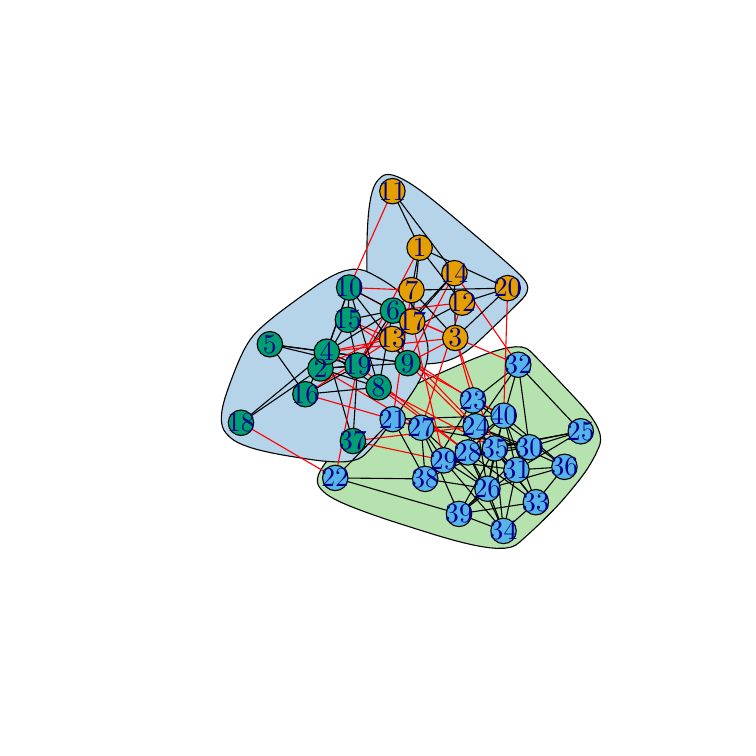
\begin{tikzpicture}[x=1pt,y=1pt]
\definecolor{fillColor}{RGB}{255,255,255}
\path[use as bounding box,fill=fillColor,fill opacity=0.00] (0,0) rectangle (252.94,252.94);
\begin{scope}
\path[clip] ( 49.20, 61.20) rectangle (227.75,203.75);
\definecolor{drawColor}{RGB}{0,0,0}
\definecolor{fillColor}{RGB}{181,211,233}

\path[draw=drawColor,line width= 0.4pt,line join=round,line cap=round,fill=fillColor] (133.18,132.28) --
	(131.57,132.82) --
	(130.18,133.47) --
	(129.00,134.21) --
	(128.04,134.99) --
	(127.20,135.79) --
	(126.40,136.63) --
	(125.61,137.77) --
	(124.86,139.41) --
	(124.18,141.68) --
	(123.61,144.59) --
	(123.52,145.18) --
	(123.18,147.88) --
	(122.93,150.88) --
	(122.75,154.12) --
	(122.63,157.53) --
	(122.57,161.02) --
	(122.55,164.52) --
	(122.56,168.02) --
	(122.57,171.53) --
	(122.61,175.03) --
	(122.70,178.49) --
	(122.86,181.83) --
	(123.08,184.96) --
	(123.38,187.82) --
	(123.56,189.14) --
	(123.96,191.43) --
	(124.42,193.37) --
	(124.93,194.96) --
	(125.48,196.21) --
	(126.05,197.17) --
	(126.64,197.90) --
	(127.23,198.51) --
	(127.84,199.07) --
	(128.56,199.55) --
	(129.46,199.84) --
	(130.59,199.89) --
	(131.98,199.65) --
	(133.63,199.09) --
	(135.26,198.34) --
	(137.42,197.14) --
	(139.81,195.61) --
	(142.37,193.80) --
	(145.04,191.77) --
	(147.76,189.59) --
	(150.49,187.34) --
	(153.21,185.06) --
	(155.94,182.76) --
	(158.67,180.46) --
	(161.37,178.17) --
	(164.01,175.94) --
	(166.50,173.81) --
	(168.79,171.83) --
	(169.99,170.79) --
	(173.01,168.14) --
	(175.29,166.09) --
	(176.87,164.60) --
	(177.97,163.51) --
	(178.96,162.50) --
	(179.82,161.42) --
	(180.43,160.25) --
	(180.69,159.03) --
	(180.69,158.83) --
	(180.45,157.48) --
	(179.78,156.18) --
	(178.81,154.99) --
	(177.71,153.88) --
	(176.49,152.67) --
	(174.99,151.19) --
	(173.17,149.41) --
	(172.41,148.68) --
	(170.81,147.13) --
	(169.10,145.50) --
	(167.35,143.83) --
	(165.62,142.18) --
	(163.93,140.57) --
	(162.21,138.97) --
	(160.37,137.39) --
	(158.36,135.90) --
	(156.21,134.56) --
	(154.10,133.51) --
	(151.65,132.59) --
	(149.19,131.96) --
	(146.82,131.61) --
	(144.56,131.47) --
	(142.40,131.43) --
	(140.21,131.43) --
	(138.00,131.51) --
	(135.84,131.74) --
	(133.80,132.12) --
	cycle;
\definecolor{fillColor}{RGB}{182,226,176}

\path[draw=drawColor,line width= 0.4pt,line join=round,line cap=round,fill=fillColor] (166.69, 65.03) --
	(163.86, 65.45) --
	(160.72, 66.06) --
	(157.36, 66.84) --
	(153.82, 67.76) --
	(150.19, 68.79) --
	(146.52, 69.90) --
	(142.86, 71.04) --
	(139.21, 72.19) --
	(135.55, 73.35) --
	(131.90, 74.53) --
	(128.31, 75.72) --
	(124.85, 76.91) --
	(121.60, 78.08) --
	(118.61, 79.20) --
	(116.65, 79.97) --
	(113.56, 81.28) --
	(111.09, 82.47) --
	(109.23, 83.51) --
	(107.91, 84.40) --
	(107.00, 85.19) --
	(106.26, 85.92) --
	(105.58, 86.69) --
	(105.04, 87.57) --
	(104.73, 88.62) --
	(104.71, 89.82) --
	(105.01, 91.19) --
	(105.13, 91.53) --
	(105.96, 93.24) --
	(107.17, 95.07) --
	(108.68, 96.97) --
	(110.39, 98.86) --
	(112.18,100.72) --
	(114.00,102.58) --
	(115.85,104.47) --
	(117.71,106.37) --
	(119.52,108.21) --
	(121.23,109.95) --
	(121.46,110.18) --
	(123.21,111.96) --
	(124.70,113.47) --
	(125.93,114.70) --
	(126.95,115.72) --
	(127.90,116.66) --
	(129.13,117.72) --
	(130.93,118.99) --
	(133.43,120.51) --
	(135.76,121.79) --
	(138.20,123.04) --
	(140.90,124.37) --
	(143.81,125.73) --
	(146.85,127.12) --
	(149.95,128.49) --
	(153.05,129.84) --
	(156.14,131.18) --
	(159.24,132.50) --
	(162.33,133.76) --
	(165.37,134.91) --
	(168.28,135.91) --
	(170.99,136.70) --
	(173.42,137.26) --
	(176.31,137.63) --
	(178.56,137.54) --
	(180.18,137.05) --
	(181.32,136.29) --
	(182.22,135.41) --
	(183.17,134.45) --
	(184.34,133.26) --
	(185.76,131.80) --
	(187.45,130.05) --
	(187.92,129.55) --
	(189.60,127.79) --
	(191.42,125.88) --
	(193.30,123.88) --
	(195.20,121.87) --
	(197.07,119.88) --
	(198.92,117.90) --
	(200.75,115.89) --
	(202.47,113.83) --
	(204.01,111.77) --
	(205.28,109.76) --
	(206.03,108.29) --
	(206.80,106.11) --
	(207.04,104.19) --
	(206.84,102.55) --
	(206.34,101.16) --
	(205.74, 99.85) --
	(205.08, 98.47) --
	(204.31, 96.99) --
	(203.42, 95.43) --
	(202.70, 94.26) --
	(201.57, 92.54) --
	(200.38, 90.89) --
	(199.20, 89.35) --
	(198.06, 87.92) --
	(196.91, 86.51) --
	(195.69, 85.03) --
	(194.40, 83.50) --
	(193.08, 81.99) --
	(192.96, 81.85) --
	(191.57, 80.32) --
	(190.26, 78.92) --
	(189.07, 77.71) --
	(187.97, 76.61) --
	(186.84, 75.48) --
	(185.56, 74.23) --
	(184.15, 72.88) --
	(183.36, 72.13) --
	(182.17, 71.03) --
	(180.97, 69.93) --
	(179.80, 68.87) --
	(178.68, 67.87) --
	(177.61, 66.91) --
	(176.42, 66.00) --
	(174.76, 65.27) --
	(172.41, 64.84) --
	(169.26, 64.80) --
	cycle;
\definecolor{fillColor}{RGB}{181,211,233}

\path[draw=drawColor,line width= 0.4pt,line join=round,line cap=round,fill=fillColor] (114.19, 96.06) --
	(111.77, 96.02) --
	(109.08, 96.14) --
	(106.19, 96.39) --
	(103.20, 96.76) --
	(100.18, 97.21) --
	( 97.17, 97.69) --
	( 94.16, 98.18) --
	( 91.14, 98.71) --
	( 88.15, 99.29) --
	( 85.28, 99.92) --
	( 82.61,100.59) --
	( 80.42,101.24) --
	( 77.94,102.12) --
	( 75.94,103.02) --
	( 74.42,103.91) --
	( 73.31,104.76) --
	( 72.45,105.59) --
	( 71.65,106.45) --
	( 70.92,107.48) --
	( 70.36,108.80) --
	( 70.04,110.42) --
	( 69.97,112.21) --
	( 70.17,114.32) --
	( 70.62,116.63) --
	( 71.27,119.06) --
	( 72.07,121.52) --
	( 72.95,123.97) --
	( 73.85,126.41) --
	( 74.79,128.87) --
	( 75.78,131.32) --
	( 76.81,133.68) --
	( 77.85,135.86) --
	( 78.18,136.50) --
	( 79.43,138.73) --
	( 80.63,140.53) --
	( 81.72,141.90) --
	( 82.73,142.96) --
	( 83.73,143.96) --
	( 84.97,145.12) --
	( 86.61,146.54) --
	( 88.70,148.25) --
	( 89.59,148.96) --
	( 91.55,150.47) --
	( 93.69,152.08) --
	( 95.94,153.74) --
	( 98.24,155.41) --
	(100.53,157.06) --
	(102.81,158.68) --
	(105.12,160.29) --
	(107.48,161.80) --
	(109.86,163.15) --
	(112.22,164.26) --
	(114.47,165.07) --
	(114.81,165.16) --
	(117.52,165.65) --
	(119.91,165.59) --
	(121.94,165.07) --
	(123.69,164.27) --
	(125.35,163.40) --
	(127.05,162.46) --
	(128.79,161.43) --
	(130.50,160.34) --
	(131.29,159.80) --
	(132.99,158.54) --
	(134.47,157.30) --
	(135.72,156.15) --
	(136.81,155.07) --
	(137.90,153.91) --
	(139.03,152.51) --
	(140.15,150.80) --
	(140.79,149.64) --
	(141.63,147.84) --
	(142.39,145.92) --
	(143.05,143.97) --
	(143.61,142.06) --
	(144.14,140.17) --
	(144.55,138.14) --
	(144.69,135.85) --
	(144.45,133.28) --
	(143.83,130.73) --
	(142.98,128.38) --
	(141.86,125.97) --
	(140.53,123.55) --
	(139.05,121.19) --
	(137.50,118.90) --
	(135.93,116.66) --
	(134.34,114.41) --
	(132.72,112.14) --
	(131.10,109.91) --
	(129.52,107.78) --
	(128.03,105.82) --
	(127.86,105.60) --
	(126.26,103.59) --
	(124.87,101.92) --
	(123.70,100.60) --
	(122.71, 99.57) --
	(121.83, 98.68) --
	(120.82, 97.83) --
	(119.44, 97.08) --
	(117.54, 96.49) --
	(115.09, 96.12) --
	cycle;

\path[draw=drawColor,line width= 0.4pt,line join=round,line cap=round] (147.25, 92.77) --
	(147.43, 92.92) --
	(148.43, 93.72) --
	(150.27, 95.21) --
	(152.36, 96.90) --
	(154.24, 98.41) --
	(155.81, 99.68) --
	(157.17,100.77) --
	(157.83,101.30) --
	(159.14,102.36) --
	(160.58,103.52) --
	(162.29,104.90) --
	(164.31,106.53) --
	(166.36,108.19) --
	(167.85,109.38) --
	(168.39,109.82) --
	(168.41,109.84);

\path[draw=drawColor,line width= 0.4pt,line join=round,line cap=round] (115.75, 90.19) --
	(115.99, 90.19) --
	(117.32, 90.17) --
	(119.62, 90.15) --
	(122.08, 90.12) --
	(124.18, 90.10) --
	(125.91, 90.08) --
	(127.40, 90.06) --
	(128.96, 90.05) --
	(130.71, 90.03) --
	(132.82, 90.00) --
	(135.29, 89.97) --
	(137.57, 89.95) --
	(138.84, 89.94) --
	(139.06, 89.93);

\path[draw=drawColor,line width= 0.4pt,line join=round,line cap=round] (190.44, 97.21) --
	(190.24, 97.38) --
	(189.19, 98.26) --
	(187.51, 99.68) --
	(185.85,101.07) --
	(184.50,102.21) --
	(183.37,103.16) --
	(182.98,103.49) --
	(181.89,104.41) --
	(180.63,105.46) --
	(179.08,106.77) --
	(177.34,108.23) --
	(175.99,109.37) --
	(175.53,109.75) --
	(175.52,109.76);

\path[draw=drawColor,line width= 0.4pt,line join=round,line cap=round] (181.23, 93.43) --
	(181.44, 93.44) --
	(182.39, 93.51) --
	(183.58, 93.58) --
	(184.53, 93.64) --
	(185.30, 93.69) --
	(186.07, 93.74) --
	(187.02, 93.80) --
	(188.21, 93.88) --
	(189.16, 93.94) --
	(189.37, 93.95);

\path[draw=drawColor,line width= 0.4pt,line join=round,line cap=round] (166.63, 96.89) --
	(166.50, 96.65) --
	(165.84, 95.43) --
	(164.81, 93.56) --
	(163.84, 91.80) --
	(163.07, 90.38) --
	(162.40, 89.17) --
	(162.35, 89.08) --
	(161.69, 87.88) --
	(160.93, 86.49) --
	(159.98, 84.75) --
	(158.94, 82.86) --
	(158.23, 81.57) --
	(158.07, 81.27) --
	(158.07, 81.27);

\path[draw=drawColor,line width= 0.4pt,line join=round,line cap=round] (164.63, 99.07) --
	(164.38, 98.97) --
	(163.12, 98.41) --
	(161.14, 97.55) --
	(159.26, 96.72) --
	(157.75, 96.06) --
	(156.46, 95.49) --
	(156.26, 95.40) --
	(154.98, 94.84) --
	(153.52, 94.20) --
	(151.69, 93.40) --
	(149.69, 92.52) --
	(148.26, 91.90) --
	(147.88, 91.73) --
	(147.88, 91.73);

\path[draw=drawColor,line width= 0.4pt,line join=round,line cap=round] (167.64, 72.73) --
	(167.44, 72.80) --
	(166.57, 73.14) --
	(165.48, 73.56) --
	(164.61, 73.89) --
	(163.90, 74.16) --
	(163.19, 74.43) --
	(162.32, 74.76) --
	(161.23, 75.18) --
	(160.35, 75.52) --
	(160.16, 75.59);

\path[draw=drawColor,line width= 0.4pt,line join=round,line cap=round] (171.46, 75.66) --
	(171.44, 75.92) --
	(171.30, 77.27) --
	(171.07, 79.50) --
	(170.83, 81.76) --
	(170.64, 83.63) --
	(170.48, 85.18) --
	(170.39, 86.00) --
	(170.24, 87.47) --
	(170.07, 89.14) --
	(169.86, 91.18) --
	(169.61, 93.52) --
	(169.41, 95.47) --
	(169.33, 96.29) --
	(169.32, 96.34);

\path[draw=drawColor,line width= 0.4pt,line join=round,line cap=round] (182.02, 85.78) --
	(181.94, 86.01) --
	(181.48, 87.25) --
	(180.67, 89.42) --
	(179.79, 91.78) --
	(179.03, 93.81) --
	(178.41, 95.49) --
	(177.85, 96.98) --
	(177.81, 97.10) --
	(177.26, 98.59) --
	(176.64,100.24) --
	(175.90,102.24) --
	(175.03,104.58) --
	(174.20,106.80) --
	(173.71,108.13) --
	(173.60,108.41) --
	(173.60,108.41);

\path[draw=drawColor,line width= 0.4pt,line join=round,line cap=round] (179.07, 80.77) --
	(178.81, 80.73) --
	(177.45, 80.53) --
	(175.30, 80.20) --
	(173.21, 79.88) --
	(171.52, 79.62) --
	(170.10, 79.41) --
	(169.74, 79.35) --
	(168.35, 79.14) --
	(166.75, 78.90) --
	(164.76, 78.59) --
	(162.56, 78.26) --
	(160.91, 78.01) --
	(160.41, 77.93) --
	(160.41, 77.93);

\path[draw=drawColor,line width= 0.4pt,line join=round,line cap=round] (118.92,126.27) --
	(118.90,125.99) --
	(118.81,124.62) --
	(118.68,122.47) --
	(118.56,120.44) --
	(118.46,118.80) --
	(118.37,117.40) --
	(118.36,117.22) --
	(118.28,115.84) --
	(118.18,114.25) --
	(118.06,112.27) --
	(117.92,110.09) --
	(117.83,108.56) --
	(117.81,108.18) --
	(117.81,108.18);

\path[draw=drawColor,line width= 0.4pt,line join=round,line cap=round] (180.84, 85.13) --
	(180.66, 85.37) --
	(179.82, 86.48) --
	(178.61, 88.08) --
	(177.55, 89.47) --
	(176.71, 90.58) --
	(176.24, 91.20) --
	(175.47, 92.21) --
	(174.56, 93.41) --
	(173.41, 94.92) --
	(172.26, 96.43) --
	(171.68, 97.20) --
	(171.63, 97.26);

\path[draw=drawColor,line width= 0.4pt,line join=round,line cap=round] (180.18, 78.41) --
	(180.06, 78.30) --
	(179.50, 77.80) --
	(178.80, 77.18) --
	(178.24, 76.68) --
	(177.78, 76.28) --
	(177.33, 75.87) --
	(176.77, 75.37) --
	(176.07, 74.75) --
	(175.51, 74.25) --
	(175.38, 74.14);

\path[draw=drawColor,line width= 0.4pt,line join=round,line cap=round] (176.04,126.70) --
	(175.98,126.46) --
	(175.62,125.17) --
	(175.00,122.97) --
	(174.36,120.69) --
	(173.83,118.76) --
	(173.38,117.17) --
	(173.07,116.03) --
	(172.66,114.56) --
	(172.20,112.91) --
	(171.63,110.90) --
	(170.98,108.57) --
	(170.41,106.51) --
	(170.12,105.48) --
	(170.09,105.36);

\path[draw=drawColor,line width= 0.4pt,line join=round,line cap=round] (175.57, 97.62) --
	(175.50, 97.90) --
	(175.21, 99.14) --
	(174.85,100.69) --
	(174.55,101.92) --
	(174.31,102.93) --
	(174.08,103.94) --
	(173.78,105.18) --
	(173.42,106.73) --
	(173.12,107.97) --
	(173.06,108.25);

\path[draw=drawColor,line width= 0.4pt,line join=round,line cap=round] (172.97, 90.34) --
	(172.75, 90.17) --
	(171.65, 89.32) --
	(169.98, 88.05) --
	(168.45, 86.88) --
	(167.23, 85.94) --
	(166.24, 85.19) --
	(165.18, 84.37) --
	(163.94, 83.42) --
	(162.39, 82.24) --
	(160.74, 80.97) --
	(159.70, 80.17) --
	(159.51, 80.03);
\definecolor{drawColor}{RGB}{255,0,0}

\path[draw=drawColor,line width= 0.4pt,line join=round,line cap=round] (140.59,128.49) --
	(140.72,128.36) --
	(141.51,127.58) --
	(143.19,125.94) --
	(145.52,123.66) --
	(148.03,121.19) --
	(150.37,118.90) --
	(152.41,116.89) --
	(154.19,115.15) --
	(155.80,113.57) --
	(156.97,112.42) --
	(158.52,110.90) --
	(160.15,109.30) --
	(161.99,107.50) --
	(164.11,105.42) --
	(166.51,103.07) --
	(169.01,100.61) --
	(171.22, 98.44) --
	(172.69, 97.00) --
	(173.28, 96.42) --
	(173.34, 96.36);
\definecolor{drawColor}{RGB}{0,0,0}

\path[draw=drawColor,line width= 0.4pt,line join=round,line cap=round] (173.38, 96.39) --
	(173.34, 96.43) --
	(173.19, 96.57) --
	(173.01, 96.76) --
	(172.86, 96.91) --
	(172.74, 97.03) --
	(172.62, 97.15) --
	(172.47, 97.30) --
	(172.29, 97.48) --
	(172.14, 97.63) --
	(172.10, 97.67);

\path[draw=drawColor,line width= 0.4pt,line join=round,line cap=round] (175.67, 88.63) --
	(175.61, 88.33) --
	(175.32, 86.95) --
	(174.93, 85.13) --
	(174.60, 83.62) --
	(174.35, 82.41) --
	(174.28, 82.11) --
	(174.04, 80.94) --
	(173.73, 79.52) --
	(173.35, 77.74) --
	(173.01, 76.14) --
	(172.90, 75.59) --
	(172.90, 75.59);

\path[draw=drawColor,line width= 0.4pt,line join=round,line cap=round] (177.95, 98.15) --
	(177.77, 97.99) --
	(176.83, 97.09) --
	(175.13, 95.48) --
	(173.23, 93.68) --
	(171.55, 92.10) --
	(170.16, 90.78) --
	(168.95, 89.63) --
	(168.57, 89.28) --
	(167.38, 88.15) --
	(166.07, 86.90) --
	(164.49, 85.41) --
	(162.63, 83.65) --
	(160.80, 81.92) --
	(159.57, 80.75) --
	(159.21, 80.41) --
	(159.20, 80.40);

\path[draw=drawColor,line width= 0.4pt,line join=round,line cap=round] (176.69,101.17) --
	(176.60,101.17) --
	(176.22,101.16) --
	(175.75,101.14) --
	(175.38,101.13) --
	(175.07,101.12) --
	(174.76,101.11) --
	(174.38,101.10) --
	(173.91,101.08) --
	(173.54,101.07) --
	(173.45,101.07);

\path[draw=drawColor,line width= 0.4pt,line join=round,line cap=round] (180.68,105.88) --
	(180.64,106.14) --
	(180.46,107.48) --
	(180.16,109.70) --
	(179.86,111.96) --
	(179.61,113.83) --
	(179.40,115.38) --
	(179.29,116.23) --
	(179.09,117.69) --
	(178.87,119.35) --
	(178.59,121.40) --
	(178.28,123.73) --
	(178.01,125.68) --
	(177.90,126.52) --
	(177.90,126.57);

\path[draw=drawColor,line width= 0.4pt,line join=round,line cap=round] (179.01, 97.32) --
	(179.01, 97.31) --
	(179.00, 97.29) --
	(178.98, 97.26) --
	(178.97, 97.24) --
	(178.96, 97.23) --
	(178.95, 97.21) --
	(178.94, 97.19) --
	(178.92, 97.16) --
	(178.91, 97.14) --
	(178.91, 97.14);

\path[draw=drawColor,line width= 0.4pt,line join=round,line cap=round] (147.09, 93.32) --
	(147.09, 93.32) --
	(147.07, 93.30) --
	(147.04, 93.27) --
	(147.02, 93.25) --
	(147.00, 93.23) --
	(146.99, 93.22) --
	(146.97, 93.19) --
	(146.94, 93.17) --
	(146.92, 93.15) --
	(146.91, 93.14);
\definecolor{drawColor}{RGB}{255,0,0}

\path[draw=drawColor,line width= 0.4pt,line join=round,line cap=round] (145.84, 97.54) --
	(145.60, 97.60) --
	(144.32, 97.87) --
	(142.04, 98.35) --
	(139.58, 98.88) --
	(137.44, 99.34) --
	(135.67, 99.71) --
	(134.10,100.05) --
	(133.94,100.08) --
	(132.38,100.42) --
	(130.64,100.79) --
	(128.55,101.23) --
	(126.10,101.76) --
	(123.76,102.25) --
	(122.35,102.56) --
	(122.03,102.62) --
	(122.03,102.62);
\definecolor{drawColor}{RGB}{0,0,0}

\path[draw=drawColor,line width= 0.4pt,line join=round,line cap=round] (154.83, 97.64) --
	(155.08, 97.69) --
	(156.19, 97.96) --
	(157.58, 98.28) --
	(158.69, 98.54) --
	(159.60, 98.75) --
	(160.50, 98.97) --
	(161.61, 99.23) --
	(163.00, 99.55) --
	(164.11, 99.81) --
	(164.37, 99.87);

\path[draw=drawColor,line width= 0.4pt,line join=round,line cap=round] (153.32, 93.07) --
	(153.48, 92.88) --
	(154.33, 91.88) --
	(155.83, 90.11) --
	(157.45, 88.19) --
	(158.86, 86.53) --
	(160.02, 85.16) --
	(161.05, 83.94) --
	(161.14, 83.83) --
	(162.17, 82.62) --
	(163.31, 81.27) --
	(164.69, 79.64) --
	(166.31, 77.73) --
	(167.84, 75.92) --
	(168.76, 74.83) --
	(168.96, 74.60) --
	(168.96, 74.60);

\path[draw=drawColor,line width= 0.4pt,line join=round,line cap=round] (154.91, 95.99) --
	(155.19, 95.95) --
	(156.56, 95.77) --
	(158.66, 95.49) --
	(160.60, 95.24) --
	(162.16, 95.03) --
	(163.49, 94.86) --
	(164.83, 94.68) --
	(166.39, 94.48) --
	(168.34, 94.22) --
	(170.43, 93.95) --
	(171.80, 93.77) --
	(172.07, 93.73);

\path[draw=drawColor,line width= 0.4pt,line join=round,line cap=round] (154.90, 97.28) --
	(155.15, 97.32) --
	(156.47, 97.52) --
	(158.72, 97.87) --
	(161.06, 98.22) --
	(163.04, 98.53) --
	(164.66, 98.77) --
	(165.82, 98.95) --
	(167.32, 99.18) --
	(169.01, 99.44) --
	(171.08, 99.75) --
	(173.46,100.12) --
	(175.57,100.44) --
	(176.62,100.60) --
	(176.74,100.62);

\path[draw=drawColor,line width= 0.4pt,line join=round,line cap=round] (162.25,102.75) --
	(162.42,102.92) --
	(163.18,103.70) --
	(164.13,104.68) --
	(164.89,105.46) --
	(165.51,106.09) --
	(166.13,106.72) --
	(166.89,107.50) --
	(167.85,108.48) --
	(168.61,109.26) --
	(168.78,109.43);

\path[draw=drawColor,line width= 0.4pt,line join=round,line cap=round] (155.12, 97.02) --
	(154.92, 96.89) --
	(154.04, 96.35) --
	(152.94, 95.66) --
	(152.06, 95.11) --
	(151.35, 94.67) --
	(150.63, 94.22) --
	(149.75, 93.67) --
	(148.65, 92.99) --
	(147.77, 92.44) --
	(147.57, 92.32);

\path[draw=drawColor,line width= 0.4pt,line join=round,line cap=round] (160.94, 95.26) --
	(161.04, 95.03) --
	(161.60, 93.81) --
	(162.54, 91.74) --
	(163.52, 89.59) --
	(164.34, 87.79) --
	(165.02, 86.30) --
	(165.48, 85.27) --
	(166.11, 83.89) --
	(166.82, 82.33) --
	(167.68, 80.44) --
	(168.68, 78.25) --
	(169.56, 76.32) --
	(169.98, 75.38) --
	(170.03, 75.27);

\path[draw=drawColor,line width= 0.4pt,line join=round,line cap=round] (162.75, 96.74) --
	(162.95, 96.58) --
	(164.04, 95.79) --
	(165.86, 94.46) --
	(167.73, 93.09) --
	(169.28, 91.96) --
	(170.56, 91.02) --
	(171.33, 90.46) --
	(172.53, 89.58) --
	(173.89, 88.58) --
	(175.57, 87.36) --
	(177.48, 85.96) --
	(179.12, 84.77) --
	(179.85, 84.23) --
	(179.91, 84.19);

\path[draw=drawColor,line width= 0.4pt,line join=round,line cap=round] (144.06,104.16) --
	(144.16,103.94) --
	(144.68,102.73) --
	(145.62,100.60) --
	(146.64, 98.26) --
	(147.54, 96.22) --
	(148.27, 94.54) --
	(148.92, 93.06) --
	(149.03, 92.80) --
	(149.68, 91.33) --
	(150.40, 89.70) --
	(151.26, 87.73) --
	(152.27, 85.42) --
	(153.25, 83.19) --
	(153.86, 81.80) --
	(154.01, 81.45) --
	(154.01, 81.45);

\path[draw=drawColor,line width= 0.4pt,line join=round,line cap=round] (142.57,103.78) --
	(142.59,103.54) --
	(142.68,102.45) --
	(142.78,101.10) --
	(142.87,100.01) --
	(142.94, 99.13) --
	(143.01, 98.25) --
	(143.09, 97.16) --
	(143.20, 95.80) --
	(143.28, 94.72) --
	(143.30, 94.47);

\path[draw=drawColor,line width= 0.4pt,line join=round,line cap=round] (136.31,110.14) --
	(136.35,110.13) --
	(136.52,110.08) --
	(136.74,110.01) --
	(136.92,109.96) --
	(137.06,109.92) --
	(137.20,109.88) --
	(137.37,109.83) --
	(137.59,109.76) --
	(137.76,109.71) --
	(137.80,109.70);
\definecolor{drawColor}{RGB}{255,0,0}

\path[draw=drawColor,line width= 0.4pt,line join=round,line cap=round] (109.78,127.45) --
	(109.96,127.35) --
	(111.01,126.73) --
	(113.08,125.51) --
	(115.62,124.01) --
	(118.07,122.58) --
	(120.17,121.34) --
	(121.95,120.29) --
	(123.57,119.34) --
	(124.01,119.08) --
	(125.60,118.14) --
	(127.32,117.13) --
	(129.33,115.95) --
	(131.69,114.56) --
	(134.25,113.06) --
	(136.52,111.72) --
	(137.87,110.93) --
	(138.24,110.71) --
	(138.24,110.71);

\path[draw=drawColor,line width= 0.4pt,line join=round,line cap=round] (136.22,148.85) --
	(136.40,148.78) --
	(137.46,148.32) --
	(139.65,147.38) --
	(142.55,146.13) --
	(145.53,144.84) --
	(148.22,143.68) --
	(150.52,142.68) --
	(152.53,141.82) --
	(154.41,141.01) --
	(154.64,140.91) --
	(156.50,140.10) --
	(158.49,139.25) --
	(160.75,138.27) --
	(163.39,137.13) --
	(166.35,135.85) --
	(169.29,134.59) --
	(171.60,133.59) --
	(172.80,133.07) --
	(173.05,132.96) --
	(173.05,132.96);
\definecolor{drawColor}{RGB}{0,0,0}

\path[draw=drawColor,line width= 0.4pt,line join=round,line cap=round] (146.74,107.56) --
	(146.96,107.52) --
	(148.19,107.29) --
	(150.54,106.87) --
	(153.34,106.36) --
	(155.97,105.89) --
	(158.19,105.49) --
	(160.08,105.15) --
	(161.75,104.85) --
	(163.50,104.53) --
	(165.40,104.19) --
	(167.64,103.78) --
	(170.28,103.31) --
	(173.08,102.80) --
	(175.39,102.38) --
	(176.57,102.17) --
	(176.76,102.13);

\path[draw=drawColor,line width= 0.4pt,line join=round,line cap=round] (144.83,104.58) --
	(144.90,104.47) --
	(145.24,103.98) --
	(145.66,103.37) --
	(146.00,102.88) --
	(146.28,102.48) --
	(146.55,102.08) --
	(146.89,101.59) --
	(147.31,100.98) --
	(147.65,100.48) --
	(147.73,100.37);

\path[draw=drawColor,line width= 0.4pt,line join=round,line cap=round] (167.14, 90.82) --
	(167.20, 91.09) --
	(167.50, 92.44) --
	(167.97, 94.53) --
	(168.40, 96.49) --
	(168.75, 98.07) --
	(169.05, 99.42) --
	(169.07, 99.53) --
	(169.37,100.87) --
	(169.71,102.42) --
	(170.14,104.35) --
	(170.61,106.45) --
	(170.93,107.90) --
	(171.00,108.23) --
	(171.00,108.23);

\path[draw=drawColor,line width= 0.4pt,line join=round,line cap=round] (162.70, 83.28) --
	(162.61, 83.20) --
	(162.21, 82.85) --
	(161.72, 82.41) --
	(161.32, 82.06) --
	(161.00, 81.78) --
	(160.68, 81.50) --
	(160.29, 81.15) --
	(159.79, 80.71) --
	(159.40, 80.36) --
	(159.31, 80.28);

\path[draw=drawColor,line width= 0.4pt,line join=round,line cap=round] (161.60, 87.04) --
	(161.30, 87.09) --
	(159.91, 87.31) --
	(158.05, 87.61) --
	(156.50, 87.85) --
	(155.26, 88.05) --
	(154.91, 88.10) --
	(153.71, 88.29) --
	(152.28, 88.52) --
	(150.47, 88.81) --
	(148.82, 89.07) --
	(148.22, 89.16) --
	(148.21, 89.16);

\path[draw=drawColor,line width= 0.4pt,line join=round,line cap=round] (170.58, 87.59) --
	(170.83, 87.66) --
	(172.15, 88.03) --
	(174.27, 88.64) --
	(176.37, 89.24) --
	(178.08, 89.72) --
	(179.52, 90.13) --
	(180.06, 90.29) --
	(181.44, 90.68) --
	(183.02, 91.13) --
	(184.98, 91.69) --
	(187.17, 92.31) --
	(188.91, 92.81) --
	(189.52, 92.98) --
	(189.54, 92.99);

\path[draw=drawColor,line width= 0.4pt,line join=round,line cap=round] (166.99, 90.85) --
	(167.01, 91.00) --
	(167.13, 91.65) --
	(167.28, 92.45) --
	(167.40, 93.10) --
	(167.50, 93.62) --
	(167.60, 94.15) --
	(167.72, 94.80) --
	(167.86, 95.60) --
	(167.98, 96.25) --
	(168.01, 96.40);

\path[draw=drawColor,line width= 0.4pt,line join=round,line cap=round] (167.78, 82.02) --
	(167.85, 81.85) --
	(168.14, 81.07) --
	(168.51, 80.11) --
	(168.80, 79.33) --
	(169.04, 78.70) --
	(169.28, 78.08) --
	(169.58, 77.30) --
	(169.94, 76.34) --
	(170.24, 75.56) --
	(170.30, 75.39);

\path[draw=drawColor,line width= 0.4pt,line join=round,line cap=round] (162.29, 88.83) --
	(162.07, 88.97) --
	(161.13, 89.58) --
	(159.95, 90.35) --
	(159.01, 90.96) --
	(158.25, 91.45) --
	(157.48, 91.95) --
	(156.54, 92.56) --
	(155.36, 93.33) --
	(154.42, 93.94) --
	(154.21, 94.08);

\path[draw=drawColor,line width= 0.4pt,line join=round,line cap=round] (163.95, 90.37) --
	(163.88, 90.51) --
	(163.56, 91.09) --
	(163.17, 91.83) --
	(162.85, 92.41) --
	(162.59, 92.89) --
	(162.33, 93.37) --
	(162.01, 93.95) --
	(161.62, 94.69) --
	(161.30, 95.27) --
	(161.22, 95.41);

\path[draw=drawColor,line width= 0.4pt,line join=round,line cap=round] (162.76, 89.44) --
	(162.58, 89.61) --
	(161.60, 90.51) --
	(159.91, 92.07) --
	(158.10, 93.74) --
	(156.56, 95.16) --
	(155.28, 96.34) --
	(154.18, 97.35) --
	(153.03, 98.41) --
	(151.75, 99.59) --
	(150.19,101.02) --
	(148.38,102.69) --
	(146.70,104.24) --
	(145.76,105.11) --
	(145.60,105.25);

\path[draw=drawColor,line width= 0.4pt,line join=round,line cap=round] (195.35,106.20) --
	(195.10,106.15) --
	(193.79,105.89) --
	(191.55,105.44) --
	(189.20,104.98) --
	(187.22,104.58) --
	(185.58,104.25) --
	(184.35,104.01) --
	(182.85,103.71) --
	(181.17,103.38) --
	(179.11,102.97) --
	(176.73,102.49) --
	(174.60,102.07) --
	(173.50,101.85) --
	(173.36,101.82);

\path[draw=drawColor,line width= 0.4pt,line join=round,line cap=round] (196.71,110.45) --
	(196.54,110.63) --
	(195.64,111.60) --
	(194.05,113.28) --
	(192.35,115.10) --
	(190.89,116.65) --
	(189.68,117.94) --
	(188.60,119.09) --
	(188.57,119.12) --
	(187.49,120.27) --
	(186.29,121.55) --
	(184.83,123.10) --
	(183.13,124.91) --
	(181.54,126.60) --
	(180.61,127.59) --
	(180.43,127.78) --
	(180.43,127.78);

\path[draw=drawColor,line width= 0.4pt,line join=round,line cap=round] (195.92,104.73) --
	(195.68,104.59) --
	(194.49,103.87) --
	(192.66,102.77) --
	(190.93,101.73) --
	(189.54,100.90) --
	(188.36,100.18) --
	(188.25,100.12) --
	(187.07, 99.41) --
	(185.71, 98.59) --
	(184.01, 97.57) --
	(182.16, 96.46) --
	(180.88, 95.69) --
	(180.58, 95.51) --
	(180.58, 95.51);

\path[draw=drawColor,line width= 0.4pt,line join=round,line cap=round] (195.34,106.25) --
	(195.12,106.21) --
	(193.92,105.98) --
	(191.56,105.54) --
	(188.69,105.01) --
	(185.94,104.49) --
	(183.60,104.05) --
	(181.60,103.68) --
	(179.79,103.34) --
	(179.45,103.28) --
	(177.65,102.94) --
	(175.70,102.57) --
	(173.43,102.15) --
	(170.76,101.65) --
	(167.86,101.11) --
	(165.35,100.64) --
	(163.90,100.37) --
	(163.56,100.30) --
	(163.56,100.30);
\definecolor{drawColor}{RGB}{255,0,0}

\path[draw=drawColor,line width= 0.4pt,line join=round,line cap=round] (157.28,108.36) --
	(157.08,108.33) --
	(155.89,108.19) --
	(153.51,107.91) --
	(150.50,107.54) --
	(147.53,107.19) --
	(144.94,106.88) --
	(142.74,106.61) --
	(140.78,106.38) --
	(139.69,106.25) --
	(137.79,106.02) --
	(135.75,105.77) --
	(133.40,105.49) --
	(130.63,105.16) --
	(127.58,104.79) --
	(124.74,104.45) --
	(122.83,104.22) --
	(122.14,104.14) --
	(122.10,104.13);
\definecolor{drawColor}{RGB}{0,0,0}

\path[draw=drawColor,line width= 0.4pt,line join=round,line cap=round] (166.04,107.00) --
	(166.26,106.90) --
	(167.44,106.36) --
	(169.57,105.38) --
	(171.97,104.29) --
	(174.09,103.32) --
	(175.84,102.52) --
	(177.38,101.82) --
	(177.91,101.58) --
	(179.41,100.89) --
	(181.06,100.14) --
	(183.05, 99.23) --
	(185.38, 98.17) --
	(187.70, 97.11) --
	(189.27, 96.39) --
	(189.77, 96.17) --
	(189.78, 96.16);

\path[draw=drawColor,line width= 0.4pt,line join=round,line cap=round] (164.71,105.30) --
	(164.86,105.11) --
	(165.67,104.10) --
	(167.13,102.26) --
	(168.75,100.21) --
	(170.19, 98.40) --
	(171.38, 96.90) --
	(172.42, 95.59) --
	(172.74, 95.19) --
	(173.76, 93.90) --
	(174.89, 92.48) --
	(176.24, 90.78) --
	(177.82, 88.78) --
	(179.39, 86.80) --
	(180.44, 85.48) --
	(180.76, 85.08) --
	(180.76, 85.08);

\path[draw=drawColor,line width= 0.4pt,line join=round,line cap=round] (164.48,112.69) --
	(164.63,112.92) --
	(165.42,114.05) --
	(166.64,115.81) --
	(167.79,117.46) --
	(168.71,118.79) --
	(169.50,119.93) --
	(169.57,120.02) --
	(170.35,121.15) --
	(171.26,122.45) --
	(172.39,124.08) --
	(173.61,125.85) --
	(174.46,127.07) --
	(174.66,127.35) --
	(174.66,127.35);

\path[draw=drawColor,line width= 0.4pt,line join=round,line cap=round] (166.14,107.23) --
	(166.43,107.12) --
	(167.70,106.63) --
	(169.28,106.01) --
	(170.54,105.51) --
	(171.57,105.11) --
	(172.60,104.71) --
	(173.87,104.22) --
	(175.45,103.60) --
	(176.71,103.10) --
	(177.00,102.99);

\path[draw=drawColor,line width= 0.4pt,line join=round,line cap=round] (160.54,104.50) --
	(160.53,104.48) --
	(160.51,104.41) --
	(160.48,104.31) --
	(160.46,104.24) --
	(160.44,104.18) --
	(160.42,104.12) --
	(160.40,104.05) --
	(160.37,103.95) --
	(160.35,103.88) --
	(160.35,103.86);

\path[draw=drawColor,line width= 0.4pt,line join=round,line cap=round] (157.25,108.78) --
	(156.98,108.77) --
	(155.76,108.74) --
	(154.24,108.70) --
	(153.02,108.67) --
	(152.03,108.64) --
	(151.04,108.61) --
	(149.83,108.58) --
	(148.31,108.54) --
	(147.09,108.51) --
	(146.81,108.50);

\path[draw=drawColor,line width= 0.4pt,line join=round,line cap=round] (165.03,116.20) --
	(165.11,116.17) --
	(165.44,116.00) --
	(165.86,115.79) --
	(166.19,115.63) --
	(166.46,115.49) --
	(166.73,115.36) --
	(167.06,115.19) --
	(167.47,114.99) --
	(167.80,114.82) --
	(167.88,114.78);

\path[draw=drawColor,line width= 0.4pt,line join=round,line cap=round] (158.52,114.33) --
	(158.40,114.12) --
	(157.71,112.99) --
	(156.51,111.01) --
	(155.21,108.87) --
	(154.09,107.03) --
	(153.16,105.50) --
	(152.34,104.15) --
	(152.29,104.07) --
	(151.47,102.72) --
	(150.55,101.21) --
	(149.44, 99.39) --
	(148.15, 97.26) --
	(146.93, 95.25) --
	(146.20, 94.06) --
	(146.05, 93.82) --
	(146.05, 93.82);
\definecolor{drawColor}{RGB}{255,0,0}

\path[draw=drawColor,line width= 0.4pt,line join=round,line cap=round] (119.57,144.88) --
	(119.73,144.77) --
	(120.67,144.17) --
	(122.65,142.89) --
	(125.38,141.14) --
	(128.28,139.27) --
	(130.98,137.53) --
	(133.32,136.02) --
	(135.35,134.72) --
	(137.20,133.53) --
	(138.31,132.81) --
	(140.11,131.65) --
	(142.01,130.43) --
	(144.15,129.05) --
	(146.63,127.46) --
	(149.43,125.65) --
	(152.33,123.78) --
	(154.83,122.17) --
	(156.43,121.15) --
	(157.00,120.78) --
	(157.04,120.75);
\definecolor{drawColor}{RGB}{0,0,0}

\path[draw=drawColor,line width= 0.4pt,line join=round,line cap=round] (164.64,115.55) --
	(164.82,115.43) --
	(165.82,114.70) --
	(167.75,113.29) --
	(170.10,111.59) --
	(172.32,109.98) --
	(174.21,108.60) --
	(175.82,107.43) --
	(177.29,106.36) --
	(177.44,106.25) --
	(178.90,105.19) --
	(180.49,104.04) --
	(182.35,102.69) --
	(184.54,101.10) --
	(186.89, 99.39) --
	(188.90, 97.93) --
	(190.01, 97.12) --
	(190.24, 96.95) --
	(190.24, 96.95);

\path[draw=drawColor,line width= 0.4pt,line join=round,line cap=round] (164.53,121.11) --
	(164.77,121.30) --
	(165.84,122.13) --
	(167.17,123.18) --
	(168.23,124.02) --
	(169.10,124.70) --
	(169.96,125.38) --
	(171.03,126.22) --
	(172.36,127.26) --
	(173.42,128.10) --
	(173.66,128.29);

\path[draw=drawColor,line width= 0.4pt,line join=round,line cap=round] (195.47,105.73) --
	(195.21,105.65) --
	(194.07,105.29) --
	(192.64,104.85) --
	(191.50,104.50) --
	(190.58,104.21) --
	(189.65,103.92) --
	(188.51,103.56) --
	(187.08,103.12) --
	(185.94,102.77) --
	(185.69,102.69);

\path[draw=drawColor,line width= 0.4pt,line join=round,line cap=round] (160.46,113.68) --
	(160.43,113.42) --
	(160.32,112.30) --
	(160.18,110.89) --
	(160.06,109.77) --
	(159.97,108.86) --
	(159.88,107.94) --
	(159.77,106.82) --
	(159.63,105.41) --
	(159.51,104.29) --
	(159.49,104.03);

\path[draw=drawColor,line width= 0.4pt,line join=round,line cap=round] (161.66,113.72) --
	(161.70,113.47) --
	(161.91,112.16) --
	(162.29,109.89) --
	(162.68,107.48) --
	(163.02,105.42) --
	(163.30,103.72) --
	(163.53,102.29) --
	(163.78,100.76) --
	(164.07, 99.04) --
	(164.41, 96.95) --
	(164.80, 94.53) --
	(165.17, 92.30) --
	(165.37, 91.07) --
	(165.40, 90.87);
\definecolor{drawColor}{RGB}{255,0,0}

\path[draw=drawColor,line width= 0.4pt,line join=round,line cap=round] (141.34,129.50) --
	(141.54,129.40) --
	(142.63,128.80) --
	(144.73,127.65) --
	(147.22,126.29) --
	(149.55,125.01) --
	(151.52,123.93) --
	(153.20,123.02) --
	(154.65,122.22) --
	(156.21,121.37) --
	(157.90,120.44) --
	(159.89,119.35) --
	(162.24,118.07) --
	(164.73,116.70) --
	(166.77,115.59) --
	(167.80,115.03) --
	(167.96,114.94);
\definecolor{drawColor}{RGB}{0,0,0}

\path[draw=drawColor,line width= 0.4pt,line join=round,line cap=round] (115.56, 88.96) --
	(115.76, 88.90) --
	(116.89, 88.57) --
	(119.19, 87.90) --
	(122.15, 87.04) --
	(125.13, 86.17) --
	(127.76, 85.41) --
	(130.01, 84.76) --
	(131.99, 84.18) --
	(133.50, 83.74) --
	(135.38, 83.19) --
	(137.40, 82.60) --
	(139.71, 81.93) --
	(142.42, 81.14) --
	(145.44, 80.27) --
	(148.33, 79.42) --
	(150.42, 78.82) --
	(151.33, 78.55) --
	(151.44, 78.52);
\definecolor{drawColor}{RGB}{255,0,0}

\path[draw=drawColor,line width= 0.4pt,line join=round,line cap=round] (130.53,120.28) --
	(130.71,120.15) --
	(131.72,119.42) --
	(133.64,118.01) --
	(135.95,116.32) --
	(138.12,114.74) --
	(139.95,113.40) --
	(141.51,112.26) --
	(142.92,111.23) --
	(144.36,110.17) --
	(145.93,109.03) --
	(147.77,107.69) --
	(149.93,106.10) --
	(152.24,104.41) --
	(154.16,103.02) --
	(155.14,102.29) --
	(155.31,102.17);

\path[draw=drawColor,line width= 0.4pt,line join=round,line cap=round] ( 81.06,107.84) --
	( 81.25,107.73) --
	( 82.33,107.10) --
	( 84.39,105.89) --
	( 86.84,104.46) --
	( 89.13,103.12) --
	( 91.06,101.99) --
	( 92.70,101.03) --
	( 94.11,100.20) --
	( 95.64, 99.31) --
	( 97.30, 98.34) --
	( 99.26, 97.19) --
	(101.57, 95.84) --
	(104.02, 94.41) --
	(106.02, 93.24) --
	(107.01, 92.66) --
	(107.17, 92.57);
\definecolor{drawColor}{RGB}{0,0,0}

\path[draw=drawColor,line width= 0.4pt,line join=round,line cap=round] (136.50,111.61) --
	(136.72,111.62) --
	(137.97,111.66) --
	(140.35,111.73) --
	(143.22,111.82) --
	(145.92,111.91) --
	(148.20,111.98) --
	(150.14,112.04) --
	(151.93,112.10) --
	(151.95,112.10) --
	(153.74,112.15) --
	(155.68,112.21) --
	(157.96,112.29) --
	(160.65,112.37) --
	(163.52,112.46) --
	(165.91,112.54) --
	(167.17,112.58) --
	(167.40,112.58) --
	(167.40,112.58);

\path[draw=drawColor,line width= 0.4pt,line join=round,line cap=round] (134.10,107.42) --
	(134.24,107.17) --
	(134.91,105.94) --
	(135.87,104.18) --
	(136.72,102.62) --
	(137.39,101.39) --
	(137.78,100.67) --
	(138.39, 99.55) --
	(139.12, 98.22) --
	(140.03, 96.55) --
	(140.94, 94.87) --
	(141.42, 94.00) --
	(141.46, 93.93);

\path[draw=drawColor,line width= 0.4pt,line join=round,line cap=round] (109.38,131.43) --
	(109.45,131.20) --
	(109.82,129.93) --
	(110.47,127.70) --
	(111.18,125.28) --
	(111.80,123.17) --
	(112.30,121.43) --
	(112.75,119.89) --
	(112.81,119.72) --
	(113.25,118.18) --
	(113.75,116.48) --
	(114.35,114.43) --
	(115.06,112.02) --
	(115.73,109.72) --
	(116.14,108.32) --
	(116.23,108.00) --
	(116.23,108.00);

\path[draw=drawColor,line width= 0.4pt,line join=round,line cap=round] (186.52, 85.05) --
	(186.64, 85.20) --
	(187.17, 85.85) --
	(187.84, 86.67) --
	(188.37, 87.33) --
	(188.80, 87.86) --
	(189.23, 88.39) --
	(189.76, 89.05) --
	(190.42, 89.86) --
	(190.95, 90.52) --
	(191.07, 90.67);
\definecolor{drawColor}{RGB}{255,0,0}

\path[draw=drawColor,line width= 0.4pt,line join=round,line cap=round] (138.04,153.55) --
	(138.01,153.35) --
	(137.84,152.18) --
	(137.50,149.82) --
	(137.05,146.75) --
	(136.60,143.65) --
	(136.19,140.90) --
	(135.85,138.55) --
	(135.55,136.49) --
	(135.30,134.78) --
	(135.02,132.83) --
	(134.71,130.74) --
	(134.36,128.34) --
	(133.95,125.54) --
	(133.50,122.41) --
	(133.06,119.39) --
	(132.73,117.17) --
	(132.59,116.16) --
	(132.57,116.02);

\path[draw=drawColor,line width= 0.4pt,line join=round,line cap=round] (155.77,136.40) --
	(155.85,136.12) --
	(156.23,134.76) --
	(156.76,132.90) --
	(157.21,131.32) --
	(157.57,130.06) --
	(157.71,129.55) --
	(158.05,128.36) --
	(158.45,126.94) --
	(158.96,125.15) --
	(159.44,123.44) --
	(159.65,122.72) --
	(159.66,122.69);
\definecolor{drawColor}{RGB}{0,0,0}

\path[draw=drawColor,line width= 0.4pt,line join=round,line cap=round] (128.68,108.18) --
	(128.50,107.99) --
	(127.55,107.02) --
	(125.99,105.42) --
	(124.42,103.82) --
	(123.12,102.49) --
	(122.05,101.39) --
	(121.52,100.85) --
	(120.50, 99.81) --
	(119.33, 98.62) --
	(117.90, 97.15) --
	(116.27, 95.48) --
	(114.93, 94.11) --
	(114.39, 93.56) --
	(114.36, 93.53);
\definecolor{drawColor}{RGB}{255,0,0}

\path[draw=drawColor,line width= 0.4pt,line join=round,line cap=round] (118.30,126.35) --
	(118.26,126.13) --
	(118.02,124.93) --
	(117.55,122.58) --
	(116.99,119.72) --
	(116.44,116.98) --
	(115.98,114.65) --
	(115.59,112.67) --
	(115.23,110.86) --
	(115.17,110.55) --
	(114.81,108.76) --
	(114.43,106.82) --
	(113.98,104.56) --
	(113.45,101.89) --
	(112.88, 99.01) --
	(112.39, 96.52) --
	(112.10, 95.09) --
	(112.04, 94.76) --
	(112.04, 94.76);

\path[draw=drawColor,line width= 0.4pt,line join=round,line cap=round] (173.31,154.23) --
	(173.30,154.02) --
	(173.26,152.84) --
	(173.19,150.45) --
	(173.09,147.37) --
	(172.99,144.30) --
	(172.91,141.59) --
	(172.84,139.28) --
	(172.77,137.24) --
	(172.73,135.78) --
	(172.66,133.83) --
	(172.60,131.74) --
	(172.52,129.34) --
	(172.43,126.53) --
	(172.33,123.40) --
	(172.24,120.42) --
	(172.17,118.31) --
	(172.15,117.42) --
	(172.14,117.33);
\definecolor{drawColor}{RGB}{0,0,0}

\path[draw=drawColor,line width= 0.4pt,line join=round,line cap=round] (104.40,122.71) --
	(104.67,122.86) --
	(105.91,123.54) --
	(107.46,124.40) --
	(108.72,125.09) --
	(109.73,125.65) --
	(109.78,125.68) --
	(110.79,126.23) --
	(112.03,126.91) --
	(113.57,127.77) --
	(114.85,128.47) --
	(115.16,128.64) --
	(115.16,128.64);
\definecolor{drawColor}{RGB}{255,0,0}

\path[draw=drawColor,line width= 0.4pt,line join=round,line cap=round] (104.79,119.21) --
	(104.99,119.15) --
	(106.15,118.81) --
	(108.45,118.15) --
	(111.33,117.31) --
	(114.14,116.50) --
	(116.57,115.80) --
	(118.64,115.20) --
	(120.49,114.66) --
	(121.29,114.43) --
	(123.10,113.91) --
	(125.05,113.34) --
	(127.30,112.69) --
	(129.96,111.92) --
	(132.87,111.08) --
	(135.52,110.31) --
	(137.22,109.82) --
	(137.77,109.66) --
	(137.79,109.65);
\definecolor{drawColor}{RGB}{0,0,0}

\path[draw=drawColor,line width= 0.4pt,line join=round,line cap=round] (116.65,142.86) --
	(116.70,142.67) --
	(116.88,141.79) --
	(117.11,140.70) --
	(117.30,139.83) --
	(117.45,139.12) --
	(117.60,138.40) --
	(117.78,137.53) --
	(118.02,136.44) --
	(118.20,135.56) --
	(118.24,135.37);
\definecolor{drawColor}{RGB}{255,0,0}

\path[draw=drawColor,line width= 0.4pt,line join=round,line cap=round] (156.85,160.44) --
	(156.97,160.26) --
	(157.69,159.25) --
	(159.05,157.29) --
	(160.70,154.93) --
	(162.25,152.70) --
	(163.56,150.82) --
	(164.68,149.21) --
	(165.71,147.73) --
	(165.75,147.68) --
	(166.78,146.21) --
	(167.89,144.61) --
	(169.20,142.73) --
	(170.74,140.52) --
	(172.39,138.16) --
	(173.77,136.17) --
	(174.51,135.11) --
	(174.65,134.91) --
	(174.65,134.91);
\definecolor{drawColor}{RGB}{0,0,0}

\path[draw=drawColor,line width= 0.4pt,line join=round,line cap=round] (112.29,133.96) --
	(112.36,133.93) --
	(112.68,133.79) --
	(113.07,133.61) --
	(113.39,133.47) --
	(113.64,133.36) --
	(113.90,133.24) --
	(114.21,133.10) --
	(114.61,132.92) --
	(114.92,132.78) --
	(115.00,132.75);

\path[draw=drawColor,line width= 0.4pt,line join=round,line cap=round] (151.19,160.75) --
	(150.99,160.52) --
	(150.07,159.46) --
	(148.81,158.02) --
	(147.75,156.80) --
	(146.90,155.83) --
	(146.60,155.48) --
	(145.79,154.56) --
	(144.83,153.46) --
	(143.62,152.06) --
	(142.48,150.76) --
	(142.02,150.23) --
	(142.01,150.22);

\path[draw=drawColor,line width= 0.4pt,line join=round,line cap=round] (135.21,143.48) --
	(135.22,143.49) --
	(135.25,143.52) --
	(135.30,143.55) --
	(135.33,143.58) --
	(135.36,143.61) --
	(135.38,143.63) --
	(135.42,143.66) --
	(135.46,143.70) --
	(135.49,143.72) --
	(135.50,143.73);
\definecolor{drawColor}{RGB}{255,0,0}

\path[draw=drawColor,line width= 0.4pt,line join=round,line cap=round] (127.85,137.99) --
	(127.66,137.87) --
	(126.58,137.18) --
	(124.58,135.91) --
	(122.28,134.44) --
	(120.19,133.11) --
	(118.44,132.00) --
	(116.93,131.04) --
	(116.05,130.48) --
	(114.61,129.56) --
	(113.03,128.56) --
	(111.16,127.37) --
	(108.95,125.96) --
	(106.68,124.51) --
	(104.98,123.43) --
	(104.30,122.99) --
	(104.25,122.96);

\path[draw=drawColor,line width= 0.4pt,line join=round,line cap=round] (127.51,142.28) --
	(127.31,142.37) --
	(126.42,142.75) --
	(125.32,143.23) --
	(124.44,143.61) --
	(123.72,143.92) --
	(123.00,144.22) --
	(122.12,144.61) --
	(121.01,145.08) --
	(120.13,145.46) --
	(119.93,145.55);
\definecolor{drawColor}{RGB}{0,0,0}

\path[draw=drawColor,line width= 0.4pt,line join=round,line cap=round] (134.90,143.81) --
	(135.07,143.99) --
	(135.98,144.95) --
	(137.57,146.63) --
	(139.26,148.42) --
	(140.72,149.96) --
	(141.92,151.22) --
	(142.98,152.34) --
	(144.05,153.48) --
	(145.25,154.75) --
	(146.71,156.29) --
	(148.41,158.09) --
	(149.99,159.76) --
	(150.89,160.71) --
	(151.05,160.88);

\path[draw=drawColor,line width= 0.4pt,line join=round,line cap=round] (161.37,154.97) --
	(161.57,155.04) --
	(162.47,155.32) --
	(163.59,155.68) --
	(164.49,155.97) --
	(165.22,156.20) --
	(165.95,156.43) --
	(166.84,156.72) --
	(167.96,157.08) --
	(168.86,157.36) --
	(169.07,157.43);

\path[draw=drawColor,line width= 0.4pt,line join=round,line cap=round] (152.90,151.45) --
	(152.66,151.33) --
	(151.44,150.70) --
	(149.50,149.69) --
	(147.60,148.70) --
	(146.05,147.90) --
	(144.76,147.22) --
	(144.36,147.02) --
	(143.10,146.36) --
	(141.65,145.61) --
	(139.86,144.68) --
	(137.86,143.64) --
	(136.33,142.85) --
	(135.83,142.59) --
	(135.82,142.59);

\path[draw=drawColor,line width= 0.4pt,line join=round,line cap=round] (134.57,190.19) --
	(134.71,190.01) --
	(135.48,188.99) --
	(136.91,187.10) --
	(138.56,184.92) --
	(140.05,182.94) --
	(141.30,181.30) --
	(142.37,179.87) --
	(143.00,179.04) --
	(144.03,177.68) --
	(145.16,176.19) --
	(146.50,174.42) --
	(148.08,172.33) --
	(149.70,170.19) --
	(150.92,168.58) --
	(151.40,167.94) --
	(151.44,167.89);
\definecolor{drawColor}{RGB}{255,0,0}

\path[draw=drawColor,line width= 0.4pt,line join=round,line cap=round] (120.24,156.85) --
	(120.48,156.72) --
	(121.71,156.06) --
	(123.54,155.07) --
	(125.22,154.17) --
	(126.55,153.45) --
	(127.58,152.89) --
	(128.75,152.26) --
	(130.12,151.52) --
	(131.83,150.60) --
	(133.64,149.63) --
	(134.75,149.03) --
	(134.93,148.93);
\definecolor{drawColor}{RGB}{0,0,0}

\path[draw=drawColor,line width= 0.4pt,line join=round,line cap=round] (115.99,154.43) --
	(115.99,154.37) --
	(115.98,154.08) --
	(115.96,153.72) --
	(115.95,153.43) --
	(115.94,153.20) --
	(115.93,152.97) --
	(115.92,152.68) --
	(115.90,152.32) --
	(115.89,152.03) --
	(115.89,151.97);
\definecolor{drawColor}{RGB}{255,0,0}

\path[draw=drawColor,line width= 0.4pt,line join=round,line cap=round] (118.07,163.24) --
	(118.16,163.44) --
	(118.68,164.60) --
	(119.65,166.77) --
	(120.79,169.31) --
	(121.83,171.64) --
	(122.71,173.59) --
	(123.46,175.27) --
	(123.99,176.45) --
	(124.70,178.03) --
	(125.47,179.76) --
	(126.39,181.80) --
	(127.47,184.22) --
	(128.60,186.73) --
	(129.47,188.69) --
	(129.87,189.57) --
	(129.91,189.66);

\path[draw=drawColor,line width= 0.4pt,line join=round,line cap=round] (139.43,135.80) --
	(139.54,136.00) --
	(140.13,137.14) --
	(141.22,139.24) --
	(142.47,141.64) --
	(143.59,143.80) --
	(144.53,145.60) --
	(145.34,147.16) --
	(145.76,147.97) --
	(146.54,149.47) --
	(147.40,151.11) --
	(148.41,153.07) --
	(149.62,155.38) --
	(150.84,157.73) --
	(151.73,159.45) --
	(152.07,160.10) --
	(152.09,160.14);
\definecolor{drawColor}{RGB}{0,0,0}

\path[draw=drawColor,line width= 0.4pt,line join=round,line cap=round] (122.23,122.56) --
	(121.96,122.54) --
	(120.57,122.41) --
	(118.47,122.21) --
	(116.51,122.02) --
	(114.94,121.87) --
	(113.59,121.74) --
	(113.59,121.74) --
	(112.24,121.62) --
	(110.68,121.47) --
	(108.72,121.28) --
	(106.61,121.08) --
	(105.23,120.95) --
	(104.95,120.92) --
	(104.95,120.92);
\definecolor{drawColor}{RGB}{255,0,0}

\path[draw=drawColor,line width= 0.4pt,line join=round,line cap=round] (155.55,149.20) --
	(155.49,149.01) --
	(155.13,147.89) --
	(154.39,145.62) --
	(153.42,142.66) --
	(152.44,139.66) --
	(151.56,136.99) --
	(150.82,134.71) --
	(150.17,132.71) --
	(149.60,130.97) --
	(148.98,129.08) --
	(148.32,127.07) --
	(147.57,124.76) --
	(146.68,122.06) --
	(145.70,119.04) --
	(144.74,116.11) --
	(144.02,113.92) --
	(143.69,112.90) --
	(143.64,112.75);
\definecolor{drawColor}{RGB}{0,0,0}

\path[draw=drawColor,line width= 0.4pt,line join=round,line cap=round] (125.51,127.41) --
	(125.45,127.63) --
	(125.09,128.85) --
	(124.42,131.13) --
	(123.64,133.77) --
	(122.93,136.18) --
	(122.33,138.19) --
	(121.82,139.92) --
	(121.50,141.02) --
	(121.01,142.66) --
	(120.48,144.47) --
	(119.85,146.60) --
	(119.11,149.12) --
	(118.34,151.73) --
	(117.75,153.72) --
	(117.51,154.55) --
	(117.49,154.62);
\definecolor{drawColor}{RGB}{255,0,0}

\path[draw=drawColor,line width= 0.4pt,line join=round,line cap=round] (136.02,154.36) --
	(135.88,154.16) --
	(135.12,153.09) --
	(133.76,151.20) --
	(132.29,149.15) --
	(131.02,147.38) --
	(129.98,145.91) --
	(129.04,144.61) --
	(128.95,144.48) --
	(128.02,143.19) --
	(126.99,141.75) --
	(125.75,140.01) --
	(124.29,137.97) --
	(122.90,136.04) --
	(122.06,134.86) --
	(121.88,134.61) --
	(121.88,134.61);
\definecolor{drawColor}{RGB}{0,0,0}

\path[draw=drawColor,line width= 0.4pt,line join=round,line cap=round] (138.82,153.50) --
	(138.82,153.44) --
	(138.82,153.19) --
	(138.83,152.88) --
	(138.84,152.63) --
	(138.84,152.42) --
	(138.85,152.22) --
	(138.85,151.97) --
	(138.86,151.66) --
	(138.87,151.41) --
	(138.87,151.35);
\definecolor{drawColor}{RGB}{255,0,0}

\path[draw=drawColor,line width= 0.4pt,line join=round,line cap=round] (134.10,158.29) --
	(133.80,158.31) --
	(132.39,158.36) --
	(130.53,158.44) --
	(128.98,158.50) --
	(127.75,158.56) --
	(127.44,158.57) --
	(126.25,158.62) --
	(124.80,158.68) --
	(122.98,158.75) --
	(121.35,158.82) --
	(120.79,158.84) --
	(120.78,158.84);
\definecolor{drawColor}{RGB}{0,0,0}

\path[draw=drawColor,line width= 0.4pt,line join=round,line cap=round] (157.85,144.01) --
	(158.05,144.20) --
	(159.06,145.16) --
	(160.58,146.60) --
	(161.97,147.92) --
	(163.09,148.98) --
	(163.98,149.83) --
	(164.95,150.75) --
	(166.08,151.83) --
	(167.50,153.17) --
	(169.00,154.60) --
	(169.95,155.50) --
	(170.11,155.66);

\path[draw=drawColor,line width= 0.4pt,line join=round,line cap=round] (129.50,146.81) --
	(129.33,146.56) --
	(128.57,145.38) --
	(127.52,143.75) --
	(126.61,142.35) --
	(125.90,141.24) --
	(125.59,140.77) --
	(124.92,139.73) --
	(124.12,138.49) --
	(123.11,136.92) --
	(122.14,135.41) --
	(121.71,134.76) --
	(121.69,134.73);
\definecolor{drawColor}{RGB}{255,0,0}

\path[draw=drawColor,line width= 0.4pt,line join=round,line cap=round] (136.01,148.42) --
	(135.98,148.44) --
	(135.86,148.50) --
	(135.71,148.59) --
	(135.58,148.66) --
	(135.49,148.71) --
	(135.39,148.77) --
	(135.27,148.84) --
	(135.12,148.92) --
	(134.99,148.99) --
	(134.97,149.00);
\definecolor{drawColor}{RGB}{0,0,0}

\path[draw=drawColor,line width= 0.4pt,line join=round,line cap=round] (127.48,149.76) --
	(127.29,149.72) --
	(126.44,149.55) --
	(125.38,149.33) --
	(124.54,149.16) --
	(123.85,149.02) --
	(123.16,148.88) --
	(122.31,148.71) --
	(121.25,148.50) --
	(120.40,148.32) --
	(120.21,148.28);
\definecolor{drawColor}{RGB}{255,0,0}

\path[draw=drawColor,line width= 0.4pt,line join=round,line cap=round] (136.57,151.21) --
	(136.85,151.24) --
	(138.24,151.40) --
	(140.27,151.64) --
	(142.08,151.85) --
	(143.52,152.01) --
	(144.49,152.13) --
	(145.78,152.28) --
	(147.30,152.45) --
	(149.21,152.67) --
	(151.18,152.90) --
	(152.28,153.03) --
	(152.41,153.04);
\definecolor{drawColor}{RGB}{0,0,0}

\path[draw=drawColor,line width= 0.4pt,line join=round,line cap=round] (127.92,152.83) --
	(127.72,152.94) --
	(126.82,153.41) --
	(125.71,154.00) --
	(124.81,154.47) --
	(124.09,154.86) --
	(123.36,155.24) --
	(122.47,155.71) --
	(121.35,156.30) --
	(120.46,156.78) --
	(120.25,156.88);

\path[draw=drawColor,line width= 0.4pt,line join=round,line cap=round] (131.15,146.15) --
	(131.10,145.89) --
	(130.84,144.54) --
	(130.44,142.39) --
	(130.05,140.32) --
	(129.74,138.63) --
	(129.47,137.21) --
	(129.40,136.84) --
	(129.14,135.45) --
	(128.85,133.86) --
	(128.48,131.88) --
	(128.07,129.68) --
	(127.76,128.03) --
	(127.66,127.53) --
	(127.66,127.52);

\path[draw=drawColor,line width= 0.4pt,line join=round,line cap=round] ( 90.19,134.79) --
	( 90.36,134.54) --
	( 91.18,133.39) --
	( 92.24,131.90) --
	( 93.12,130.67) --
	( 93.82,129.69) --
	( 93.94,129.52) --
	( 94.62,128.56) --
	( 95.46,127.39) --
	( 96.50,125.92) --
	( 97.41,124.64) --
	( 97.69,124.24) --
	( 97.69,124.24);

\path[draw=drawColor,line width= 0.4pt,line join=round,line cap=round] ( 91.99,137.46) --
	( 92.23,137.40) --
	( 93.52,137.09) --
	( 95.76,136.54) --
	( 98.15,135.96) --
	(100.20,135.47) --
	(101.89,135.06) --
	(103.36,134.70) --
	(104.88,134.34) --
	(106.57,133.92) --
	(108.63,133.42) --
	(111.03,132.84) --
	(113.25,132.30) --
	(114.50,132.00) --
	(114.72,131.95);

\path[draw=drawColor,line width= 0.4pt,line join=round,line cap=round] ( 92.08,137.92) --
	( 92.27,137.89) --
	( 93.41,137.74) --
	( 95.76,137.41) --
	( 98.91,136.98) --
	(102.17,136.53) --
	(105.13,136.13) --
	(107.67,135.78) --
	(109.89,135.47) --
	(111.95,135.19) --
	(112.41,135.13) --
	(114.45,134.85) --
	(116.61,134.55) --
	(119.07,134.22) --
	(121.93,133.82) --
	(125.15,133.38) --
	(128.38,132.94) --
	(130.97,132.58) --
	(132.39,132.39) --
	(132.74,132.34) --
	(132.74,132.34);
\definecolor{drawColor}{RGB}{255,0,0}

\path[draw=drawColor,line width= 0.4pt,line join=round,line cap=round] (122.81,128.01) --
	(122.96,127.89) --
	(123.86,127.18) --
	(125.73,125.71) --
	(128.23,123.74) --
	(130.84,121.69) --
	(133.20,119.82) --
	(135.24,118.21) --
	(137.02,116.81) --
	(138.66,115.52) --
	(139.11,115.16) --
	(140.74,113.88) --
	(142.46,112.52) --
	(144.41,110.98) --
	(146.69,109.18) --
	(149.25,107.16) --
	(151.83,105.13) --
	(153.93,103.47) --
	(155.10,102.55) --
	(155.41,102.31) --
	(155.41,102.30);
\definecolor{drawColor}{RGB}{0,0,0}

\path[draw=drawColor,line width= 0.4pt,line join=round,line cap=round] (104.54,132.91) --
	(104.37,132.77) --
	(103.42,131.98) --
	(101.58,130.45) --
	( 99.36,128.62) --
	( 97.28,126.89) --
	( 95.51,125.43) --
	( 94.01,124.18) --
	( 92.62,123.04) --
	( 92.59,123.01) --
	( 91.20,121.86) --
	( 89.70,120.62) --
	( 87.95,119.16) --
	( 85.87,117.44) --
	( 83.65,115.61) --
	( 81.80,114.07) --
	( 80.81,113.25) --
	( 80.63,113.10) --
	( 80.63,113.10);

\path[draw=drawColor,line width= 0.4pt,line join=round,line cap=round] (106.02,131.73) --
	(105.92,131.55) --
	(105.51,130.71) --
	(104.98,129.68) --
	(104.57,128.84) --
	(104.23,128.17) --
	(103.89,127.49) --
	(103.47,126.66) --
	(102.95,125.62) --
	(102.53,124.79) --
	(102.43,124.60);
\definecolor{drawColor}{RGB}{255,0,0}

\path[draw=drawColor,line width= 0.4pt,line join=round,line cap=round] (112.61,136.73) --
	(112.89,136.79) --
	(114.27,137.06) --
	(116.21,137.43) --
	(117.90,137.76) --
	(119.23,138.02) --
	(119.91,138.16) --
	(121.15,138.40) --
	(122.62,138.68) --
	(124.47,139.05) --
	(126.29,139.40) --
	(127.16,139.57) --
	(127.22,139.58);

\path[draw=drawColor,line width= 0.4pt,line join=round,line cap=round] (140.00,142.26) --
	(140.04,142.07) --
	(140.29,140.96) --
	(140.82,138.65) --
	(141.52,135.53) --
	(142.26,132.26) --
	(142.94,129.27) --
	(143.52,126.70) --
	(144.03,124.46) --
	(144.50,122.40) --
	(144.66,121.67) --
	(145.12,119.63) --
	(145.61,117.48) --
	(146.16,115.04) --
	(146.81,112.20) --
	(147.53,109.00) --
	(148.27,105.75) --
	(148.87,103.08) --
	(149.23,101.53) --
	(149.33,101.08) --
	(149.33,101.07);
\definecolor{drawColor}{RGB}{0,0,0}

\path[draw=drawColor,line width= 0.4pt,line join=round,line cap=round] (109.60,140.19) --
	(109.70,140.47) --
	(110.16,141.79) --
	(110.82,143.69) --
	(111.41,145.35) --
	(111.87,146.68) --
	(112.13,147.44) --
	(112.56,148.65) --
	(113.05,150.07) --
	(113.68,151.87) --
	(114.31,153.68) --
	(114.64,154.61) --
	(114.66,154.69);

\path[draw=drawColor,line width= 0.4pt,line join=round,line cap=round] (112.65,135.20) --
	(112.90,135.17) --
	(114.25,134.98) --
	(116.46,134.66) --
	(118.66,134.35) --
	(120.48,134.09) --
	(122.00,133.88) --
	(122.70,133.78) --
	(124.14,133.58) --
	(125.78,133.34) --
	(127.81,133.06) --
	(130.11,132.73) --
	(131.98,132.47) --
	(132.71,132.36) --
	(132.74,132.36);

\path[draw=drawColor,line width= 0.4pt,line join=round,line cap=round] (111.88,133.24) --
	(112.13,133.07) --
	(113.30,132.27) --
	(114.84,131.21) --
	(116.14,130.32) --
	(117.17,129.62) --
	(117.45,129.42) --
	(118.44,128.74) --
	(119.64,127.92) --
	(121.15,126.89) --
	(122.52,125.95) --
	(123.01,125.61) --
	(123.02,125.60);

\path[draw=drawColor,line width= 0.4pt,line join=round,line cap=round] (112.00,138.27) --
	(112.23,138.42) --
	(113.40,139.14) --
	(115.25,140.29) --
	(117.04,141.40) --
	(118.50,142.31) --
	(119.73,143.07) --
	(120.04,143.26) --
	(121.24,144.01) --
	(122.62,144.86) --
	(124.32,145.92) --
	(126.22,147.10) --
	(127.64,147.98) --
	(128.08,148.25) --
	(128.08,148.25);

\path[draw=drawColor,line width= 0.4pt,line join=round,line cap=round] (103.52,136.45) --
	(103.22,136.49) --
	(101.88,136.66) --
	(100.22,136.88) --
	( 98.89,137.05) --
	( 97.80,137.20) --
	( 96.72,137.34) --
	( 95.38,137.51) --
	( 93.72,137.73) --
	( 92.38,137.91) --
	( 92.08,137.95);

\path[draw=drawColor,line width= 0.4pt,line join=round,line cap=round] (143.31,158.20) --
	(143.55,158.20) --
	(144.85,158.23) --
	(147.19,158.28) --
	(149.79,158.33) --
	(152.07,158.38) --
	(153.97,158.42) --
	(155.63,158.46) --
	(156.08,158.46) --
	(157.71,158.50) --
	(159.51,158.54) --
	(161.68,158.58) --
	(164.23,158.63) --
	(166.73,158.69) --
	(168.37,158.72) --
	(168.84,158.73) --
	(168.85,158.73);

\path[draw=drawColor,line width= 0.4pt,line join=round,line cap=round] (154.45,145.44) --
	(154.45,145.74) --
	(154.43,147.15) --
	(154.41,149.07) --
	(154.39,150.71) --
	(154.37,152.02) --
	(154.36,152.53) --
	(154.35,153.76) --
	(154.33,155.23) --
	(154.31,157.09) --
	(154.28,158.85) --
	(154.27,159.59) --
	(154.27,159.62);
\definecolor{drawColor}{RGB}{255,0,0}

\path[draw=drawColor,line width= 0.4pt,line join=round,line cap=round] (156.07,136.50) --
	(156.14,136.30) --
	(156.55,135.15) --
	(157.36,132.90) --
	(158.36,130.11) --
	(159.33,127.43) --
	(160.15,125.13) --
	(160.86,123.17) --
	(161.49,121.40) --
	(161.68,120.88) --
	(162.31,119.14) --
	(162.98,117.25) --
	(163.77,115.06) --
	(164.70,112.48) --
	(165.70,109.67) --
	(166.60,107.18) --
	(167.14,105.68) --
	(167.29,105.26) --
	(167.29,105.26);

\path[draw=drawColor,line width= 0.4pt,line join=round,line cap=round] (150.44,138.68) --
	(150.20,138.55) --
	(149.15,137.99) --
	(147.82,137.29) --
	(146.77,136.73) --
	(145.91,136.27) --
	(145.05,135.82) --
	(143.99,135.26) --
	(142.67,134.56) --
	(141.61,134.00) --
	(141.37,133.87);
\definecolor{drawColor}{RGB}{0,0,0}

\path[draw=drawColor,line width= 0.4pt,line join=round,line cap=round] (151.40,144.23) --
	(151.20,144.45) --
	(150.25,145.49) --
	(148.95,146.91) --
	(147.84,148.13) --
	(146.96,149.09) --
	(146.61,149.47) --
	(145.78,150.38) --
	(144.78,151.46) --
	(143.53,152.84) --
	(142.33,154.14) --
	(141.83,154.69) --
	(141.81,154.71);
\definecolor{drawColor}{RGB}{255,0,0}

\path[draw=drawColor,line width= 0.4pt,line join=round,line cap=round] (150.29,142.68) --
	(150.03,142.80) --
	(148.74,143.36) --
	(146.90,144.16) --
	(145.28,144.87) --
	(144.00,145.43) --
	(143.25,145.76) --
	(142.08,146.27) --
	(140.70,146.87) --
	(138.95,147.64) --
	(137.20,148.40) --
	(136.29,148.80) --
	(136.21,148.83);

\path[draw=drawColor,line width= 0.4pt,line join=round,line cap=round] (149.93,140.34) --
	(149.73,140.32) --
	(148.56,140.20) --
	(146.18,139.94) --
	(143.11,139.61) --
	(140.02,139.28) --
	(137.28,138.98) --
	(134.95,138.73) --
	(132.90,138.51) --
	(131.30,138.34) --
	(129.34,138.13) --
	(127.25,137.91) --
	(124.86,137.65) --
	(122.05,137.35) --
	(118.92,137.01) --
	(115.92,136.69) --
	(113.73,136.45) --
	(112.78,136.35) --
	(112.66,136.34);
\definecolor{drawColor}{RGB}{0,0,0}

\path[draw=drawColor,line width= 0.4pt,line join=round,line cap=round] (110.40,130.16) --
	(110.51,130.17) --
	(111.00,130.20) --
	(111.61,130.25) --
	(112.10,130.29) --
	(112.50,130.33) --
	(112.90,130.36) --
	(113.39,130.40) --
	(114.00,130.45) --
	(114.50,130.49) --
	(114.61,130.49);

\path[draw=drawColor,line width= 0.4pt,line join=round,line cap=round] (102.01,127.19) --
	(101.81,127.06) --
	(100.73,126.32) --
	( 98.80,125.00) --
	( 96.65,123.53) --
	( 94.76,122.24) --
	( 93.20,121.17) --
	( 91.83,120.24) --
	( 91.45,119.98) --
	( 90.10,119.06) --
	( 88.61,118.04) --
	( 86.82,116.81) --
	( 84.71,115.38) --
	( 82.65,113.97) --
	( 81.28,113.03) --
	( 80.89,112.77) --
	( 80.89,112.76);
\definecolor{drawColor}{RGB}{255,0,0}

\path[draw=drawColor,line width= 0.4pt,line join=round,line cap=round] (109.91,131.88) --
	(110.11,131.99) --
	(111.25,132.57) --
	(113.36,133.65) --
	(115.79,134.89) --
	(118.01,136.02) --
	(119.85,136.97) --
	(121.44,137.78) --
	(122.39,138.27) --
	(123.91,139.04) --
	(125.58,139.90) --
	(127.56,140.91) --
	(129.89,142.10) --
	(132.29,143.33) --
	(134.09,144.25) --
	(134.83,144.62) --
	(134.88,144.65);
\definecolor{drawColor}{RGB}{0,0,0}

\path[draw=drawColor,line width= 0.4pt,line join=round,line cap=round] (108.07,133.80) --
	(108.21,134.05) --
	(108.83,135.17) --
	(109.62,136.56) --
	(110.24,137.67) --
	(110.75,138.58) --
	(111.26,139.48) --
	(111.89,140.60) --
	(112.67,141.99) --
	(113.30,143.10) --
	(113.44,143.35);
\definecolor{drawColor}{RGB}{255,0,0}

\path[draw=drawColor,line width= 0.4pt,line join=round,line cap=round] (134.91,137.13) --
	(135.06,136.98) --
	(135.89,136.11) --
	(137.55,134.38) --
	(139.62,132.20) --
	(141.64,130.09) --
	(143.39,128.25) --
	(144.88,126.69) --
	(146.21,125.30) --
	(146.79,124.69) --
	(148.10,123.32) --
	(149.50,121.85) --
	(151.12,120.15) --
	(153.03,118.15) --
	(155.13,115.96) --
	(157.03,113.96) --
	(158.26,112.67) --
	(158.66,112.25) --
	(158.67,112.24);
\definecolor{drawColor}{RGB}{0,0,0}

\path[draw=drawColor,line width= 0.4pt,line join=round,line cap=round] (107.35,134.13) --
	(107.43,134.37) --
	(107.88,135.63) --
	(108.64,137.77) --
	(109.43,139.99) --
	(110.08,141.84) --
	(110.63,143.38) --
	(110.99,144.41) --
	(111.50,145.84) --
	(112.07,147.44) --
	(112.77,149.40) --
	(113.57,151.67) --
	(114.27,153.65) --
	(114.61,154.60) --
	(114.64,154.70);

\path[draw=drawColor,line width= 0.4pt,line join=round,line cap=round] (110.40,130.07) --
	(110.65,130.08) --
	(111.99,130.17) --
	(114.27,130.31) --
	(116.65,130.45) --
	(118.66,130.57) --
	(120.33,130.68) --
	(121.56,130.75) --
	(123.08,130.84) --
	(124.80,130.95) --
	(126.89,131.08) --
	(129.31,131.22) --
	(131.47,131.36) --
	(132.57,131.42) --
	(132.71,131.43);

\path[draw=drawColor,line width= 0.4pt,line join=round,line cap=round] (110.19,128.37) --
	(110.48,128.28) --
	(111.82,127.84) --
	(113.56,127.28) --
	(114.99,126.82) --
	(116.13,126.45) --
	(116.31,126.39) --
	(117.43,126.03) --
	(118.79,125.59) --
	(120.50,125.04) --
	(121.99,124.56) --
	(122.43,124.41) --
	(122.43,124.41);

\path[draw=drawColor,line width= 0.4pt,line join=round,line cap=round] (107.43,134.10) --
	(107.40,134.03) --
	(107.29,133.73) --
	(107.15,133.36) --
	(107.04,133.06) --
	(106.95,132.82) --
	(106.86,132.58) --
	(106.74,132.28) --
	(106.60,131.90) --
	(106.49,131.61) --
	(106.47,131.54);

\path[draw=drawColor,line width= 0.4pt,line join=round,line cap=round] (145.80,171.51) --
	(146.02,171.41) --
	(147.20,170.87) --
	(149.33,169.89) --
	(151.71,168.80) --
	(153.80,167.84) --
	(155.54,167.04) --
	(157.06,166.35) --
	(157.53,166.13) --
	(159.02,165.45) --
	(160.67,164.69) --
	(162.65,163.78) --
	(164.97,162.72) --
	(167.26,161.67) --
	(168.80,160.96) --
	(169.26,160.75) --
	(169.27,160.75);
\definecolor{drawColor}{RGB}{255,0,0}

\path[draw=drawColor,line width= 0.4pt,line join=round,line cap=round] (139.47,169.36) --
	(139.38,169.18) --
	(138.83,168.15) --
	(137.72,166.04) --
	(136.26,163.27) --
	(134.78,160.45) --
	(133.45,157.93) --
	(132.32,155.78) --
	(131.33,153.89) --
	(130.41,152.15) --
	(129.47,150.38) --
	(128.48,148.49) --
	(127.34,146.33) --
	(126.01,143.81) --
	(124.53,140.98) --
	(123.07,138.22) --
	(121.97,136.12) --
	(121.43,135.11) --
	(121.34,134.94);
\definecolor{drawColor}{RGB}{0,0,0}

\path[draw=drawColor,line width= 0.4pt,line join=round,line cap=round] (141.16,168.85) --
	(141.14,168.58) --
	(141.00,167.20) --
	(140.79,165.08) --
	(140.59,163.10) --
	(140.44,161.51) --
	(140.30,160.15) --
	(140.30,160.09) --
	(140.16,158.73) --
	(140.01,157.16) --
	(139.81,155.20) --
	(139.60,153.07) --
	(139.46,151.64) --
	(139.43,151.33) --
	(139.43,151.33);

\path[draw=drawColor,line width= 0.4pt,line join=round,line cap=round] (144.43,169.79) --
	(144.61,169.56) --
	(145.47,168.46) --
	(146.71,166.85) --
	(147.83,165.40) --
	(148.71,164.26) --
	(149.30,163.50) --
	(150.10,162.48) --
	(151.03,161.27) --
	(152.21,159.75) --
	(153.41,158.19) --
	(154.09,157.31) --
	(154.17,157.21);

\path[draw=drawColor,line width= 0.4pt,line join=round,line cap=round] (139.62,177.58) --
	(139.49,177.86) --
	(138.88,179.13) --
	(138.06,180.82) --
	(137.39,182.22) --
	(136.85,183.35) --
	(136.70,183.65) --
	(136.18,184.73) --
	(135.55,186.04) --
	(134.76,187.68) --
	(134.04,189.18) --
	(133.79,189.70) --
	(133.79,189.71);

\path[draw=drawColor,line width= 0.4pt,line join=round,line cap=round] (134.49,135.36) --
	(134.34,135.54) --
	(133.54,136.58) --
	(132.11,138.43) --
	(130.53,140.47) --
	(129.14,142.27) --
	(128.00,143.75) --
	(126.99,145.06) --
	(126.74,145.37) --
	(125.75,146.66) --
	(124.65,148.08) --
	(123.33,149.79) --
	(121.77,151.80) --
	(120.26,153.76) --
	(119.27,155.04) --
	(119.00,155.39) --
	(119.00,155.39);
\definecolor{drawColor}{RGB}{255,0,0}

\path[draw=drawColor,line width= 0.4pt,line join=round,line cap=round] (130.89,120.86) --
	(131.07,120.76) --
	(132.11,120.22) --
	(134.22,119.11) --
	(136.98,117.66) --
	(139.77,116.20) --
	(142.25,114.89) --
	(144.37,113.78) --
	(146.23,112.80) --
	(147.83,111.96) --
	(149.59,111.04) --
	(151.47,110.05) --
	(153.62,108.92) --
	(156.13,107.60) --
	(158.94,106.13) --
	(161.66,104.70) --
	(163.69,103.63) --
	(164.64,103.14) --
	(164.77,103.06);
\definecolor{drawColor}{RGB}{0,0,0}

\path[draw=drawColor,line width= 0.4pt,line join=round,line cap=round] (140.76,168.91) --
	(140.72,168.74) --
	(140.59,168.01) --
	(140.41,167.10) --
	(140.27,166.36) --
	(140.16,165.77) --
	(140.05,165.17) --
	(139.91,164.44) --
	(139.73,163.52) --
	(139.59,162.79) --
	(139.56,162.63);
\definecolor{fillColor}{RGB}{230,159,0}

\path[draw=drawColor,line width= 0.4pt,line join=round,line cap=round,fill=fillColor] (141.62,173.43) circle (  4.60);
\definecolor{fillColor}{RGB}{0,158,115}

\path[draw=drawColor,line width= 0.4pt,line join=round,line cap=round,fill=fillColor] (105.81,129.79) circle (  4.60);
\definecolor{fillColor}{RGB}{230,159,0}

\path[draw=drawColor,line width= 0.4pt,line join=round,line cap=round,fill=fillColor] (154.51,140.83) circle (  4.60);
\definecolor{fillColor}{RGB}{0,158,115}

\path[draw=drawColor,line width= 0.4pt,line join=round,line cap=round,fill=fillColor] (108.09,135.85) circle (  4.60);

\path[draw=drawColor,line width= 0.4pt,line join=round,line cap=round,fill=fillColor] ( 87.52,138.54) circle (  4.60);

\path[draw=drawColor,line width= 0.4pt,line join=round,line cap=round,fill=fillColor] (131.99,150.68) circle (  4.60);
\definecolor{fillColor}{RGB}{230,159,0}

\path[draw=drawColor,line width= 0.4pt,line join=round,line cap=round,fill=fillColor] (138.70,158.10) circle (  4.60);
\definecolor{fillColor}{RGB}{0,158,115}

\path[draw=drawColor,line width= 0.4pt,line join=round,line cap=round,fill=fillColor] (126.82,123.00) circle (  4.60);

\path[draw=drawColor,line width= 0.4pt,line join=round,line cap=round,fill=fillColor] (137.30,131.71) circle (  4.60);

\path[draw=drawColor,line width= 0.4pt,line join=round,line cap=round,fill=fillColor] (116.18,159.04) circle (  4.60);
\definecolor{fillColor}{RGB}{230,159,0}

\path[draw=drawColor,line width= 0.4pt,line join=round,line cap=round,fill=fillColor] (131.79,193.86) circle (  4.60);

\path[draw=drawColor,line width= 0.4pt,line join=round,line cap=round,fill=fillColor] (156.98,153.57) circle (  4.60);

\path[draw=drawColor,line width= 0.4pt,line join=round,line cap=round,fill=fillColor] (131.73,140.46) circle (  4.60);

\path[draw=drawColor,line width= 0.4pt,line join=round,line cap=round,fill=fillColor] (154.22,164.22) circle (  4.60);
\definecolor{fillColor}{RGB}{0,158,115}

\path[draw=drawColor,line width= 0.4pt,line join=round,line cap=round,fill=fillColor] (115.70,147.37) circle (  4.60);

\path[draw=drawColor,line width= 0.4pt,line join=round,line cap=round,fill=fillColor] (100.36,120.49) circle (  4.60);
\definecolor{fillColor}{RGB}{230,159,0}

\path[draw=drawColor,line width= 0.4pt,line join=round,line cap=round,fill=fillColor] (138.98,146.75) circle (  4.60);
\definecolor{fillColor}{RGB}{0,158,115}

\path[draw=drawColor,line width= 0.4pt,line join=round,line cap=round,fill=fillColor] ( 77.08,110.17) circle (  4.60);

\path[draw=drawColor,line width= 0.4pt,line join=round,line cap=round,fill=fillColor] (119.20,130.86) circle (  4.60);
\definecolor{fillColor}{RGB}{230,159,0}

\path[draw=drawColor,line width= 0.4pt,line join=round,line cap=round,fill=fillColor] (173.45,158.83) circle (  4.60);
\definecolor{fillColor}{RGB}{86,180,233}

\path[draw=drawColor,line width= 0.4pt,line join=round,line cap=round,fill=fillColor] (131.90,111.47) circle (  4.60);

\path[draw=drawColor,line width= 0.4pt,line join=round,line cap=round,fill=fillColor] (111.14, 90.24) circle (  4.60);

\path[draw=drawColor,line width= 0.4pt,line join=round,line cap=round,fill=fillColor] (160.92,118.26) circle (  4.60);

\path[draw=drawColor,line width= 0.4pt,line join=round,line cap=round,fill=fillColor] (161.85,108.91) circle (  4.60);

\path[draw=drawColor,line width= 0.4pt,line join=round,line cap=round,fill=fillColor] (199.86,107.10) circle (  4.60);

\path[draw=drawColor,line width= 0.4pt,line join=round,line cap=round,fill=fillColor] (166.15, 86.33) circle (  4.60);

\path[draw=drawColor,line width= 0.4pt,line join=round,line cap=round,fill=fillColor] (142.21,108.37) circle (  4.60);

\path[draw=drawColor,line width= 0.4pt,line join=round,line cap=round,fill=fillColor] (159.03, 99.45) circle (  4.60);

\path[draw=drawColor,line width= 0.4pt,line join=round,line cap=round,fill=fillColor] (150.34, 96.58) circle (  4.60);

\path[draw=drawColor,line width= 0.4pt,line join=round,line cap=round,fill=fillColor] (181.29,101.32) circle (  4.60);

\path[draw=drawColor,line width= 0.4pt,line join=round,line cap=round,fill=fillColor] (176.63, 93.14) circle (  4.60);

\path[draw=drawColor,line width= 0.4pt,line join=round,line cap=round,fill=fillColor] (177.28,131.14) circle (  4.60);

\path[draw=drawColor,line width= 0.4pt,line join=round,line cap=round,fill=fillColor] (183.63, 81.47) circle (  4.60);

\path[draw=drawColor,line width= 0.4pt,line join=round,line cap=round,fill=fillColor] (171.94, 71.08) circle (  4.60);

\path[draw=drawColor,line width= 0.4pt,line join=round,line cap=round,fill=fillColor] (168.85,100.92) circle (  4.60);

\path[draw=drawColor,line width= 0.4pt,line join=round,line cap=round,fill=fillColor] (193.97, 94.25) circle (  4.60);
\definecolor{fillColor}{RGB}{0,158,115}

\path[draw=drawColor,line width= 0.4pt,line join=round,line cap=round,fill=fillColor] (117.53,103.58) circle (  4.60);
\definecolor{fillColor}{RGB}{86,180,233}

\path[draw=drawColor,line width= 0.4pt,line join=round,line cap=round,fill=fillColor] (143.66, 89.88) circle (  4.60);

\path[draw=drawColor,line width= 0.4pt,line join=round,line cap=round,fill=fillColor] (155.86, 77.24) circle (  4.60);

\path[draw=drawColor,line width= 0.4pt,line join=round,line cap=round,fill=fillColor] (172.00,112.73) circle (  4.60);
\end{scope}
\begin{scope}
\path[clip] (  0.00,  0.00) rectangle (252.94,252.94);
\definecolor{drawColor}{RGB}{0,0,139}

\node[text=drawColor,anchor=base,inner sep=0pt, outer sep=0pt, scale=  1.00] at (141.62,170.23) {1};

\node[text=drawColor,anchor=base,inner sep=0pt, outer sep=0pt, scale=  1.00] at (105.81,126.58) {2};

\node[text=drawColor,anchor=base,inner sep=0pt, outer sep=0pt, scale=  1.00] at (154.51,137.63) {3};

\node[text=drawColor,anchor=base,inner sep=0pt, outer sep=0pt, scale=  1.00] at (108.09,132.64) {4};

\node[text=drawColor,anchor=base,inner sep=0pt, outer sep=0pt, scale=  1.00] at ( 87.52,135.34) {5};

\node[text=drawColor,anchor=base,inner sep=0pt, outer sep=0pt, scale=  1.00] at (131.99,147.47) {6};

\node[text=drawColor,anchor=base,inner sep=0pt, outer sep=0pt, scale=  1.00] at (138.70,154.89) {7};

\node[text=drawColor,anchor=base,inner sep=0pt, outer sep=0pt, scale=  1.00] at (126.82,119.79) {8};

\node[text=drawColor,anchor=base,inner sep=0pt, outer sep=0pt, scale=  1.00] at (137.30,128.51) {9};

\node[text=drawColor,anchor=base,inner sep=0pt, outer sep=0pt, scale=  1.00] at (116.18,155.83) {10};

\node[text=drawColor,anchor=base,inner sep=0pt, outer sep=0pt, scale=  1.00] at (131.79,190.65) {11};

\node[text=drawColor,anchor=base,inner sep=0pt, outer sep=0pt, scale=  1.00] at (156.98,150.37) {12};

\node[text=drawColor,anchor=base,inner sep=0pt, outer sep=0pt, scale=  1.00] at (131.73,137.26) {13};

\node[text=drawColor,anchor=base,inner sep=0pt, outer sep=0pt, scale=  1.00] at (154.22,161.01) {14};

\node[text=drawColor,anchor=base,inner sep=0pt, outer sep=0pt, scale=  1.00] at (115.70,144.16) {15};

\node[text=drawColor,anchor=base,inner sep=0pt, outer sep=0pt, scale=  1.00] at (100.36,117.28) {16};

\node[text=drawColor,anchor=base,inner sep=0pt, outer sep=0pt, scale=  1.00] at (138.98,143.54) {17};

\node[text=drawColor,anchor=base,inner sep=0pt, outer sep=0pt, scale=  1.00] at ( 77.08,106.96) {18};

\node[text=drawColor,anchor=base,inner sep=0pt, outer sep=0pt, scale=  1.00] at (119.20,127.66) {19};

\node[text=drawColor,anchor=base,inner sep=0pt, outer sep=0pt, scale=  1.00] at (173.45,155.62) {20};

\node[text=drawColor,anchor=base,inner sep=0pt, outer sep=0pt, scale=  1.00] at (131.90,108.26) {21};

\node[text=drawColor,anchor=base,inner sep=0pt, outer sep=0pt, scale=  1.00] at (111.14, 87.04) {22};

\node[text=drawColor,anchor=base,inner sep=0pt, outer sep=0pt, scale=  1.00] at (160.92,115.05) {23};

\node[text=drawColor,anchor=base,inner sep=0pt, outer sep=0pt, scale=  1.00] at (161.85,105.70) {24};

\node[text=drawColor,anchor=base,inner sep=0pt, outer sep=0pt, scale=  1.00] at (199.86,103.89) {25};

\node[text=drawColor,anchor=base,inner sep=0pt, outer sep=0pt, scale=  1.00] at (166.15, 83.12) {26};

\node[text=drawColor,anchor=base,inner sep=0pt, outer sep=0pt, scale=  1.00] at (142.21,105.17) {27};

\node[text=drawColor,anchor=base,inner sep=0pt, outer sep=0pt, scale=  1.00] at (159.03, 96.25) {28};

\node[text=drawColor,anchor=base,inner sep=0pt, outer sep=0pt, scale=  1.00] at (150.34, 93.38) {29};

\node[text=drawColor,anchor=base,inner sep=0pt, outer sep=0pt, scale=  1.00] at (181.29, 98.11) {30};

\node[text=drawColor,anchor=base,inner sep=0pt, outer sep=0pt, scale=  1.00] at (176.63, 89.93) {31};

\node[text=drawColor,anchor=base,inner sep=0pt, outer sep=0pt, scale=  1.00] at (177.28,127.93) {32};

\node[text=drawColor,anchor=base,inner sep=0pt, outer sep=0pt, scale=  1.00] at (183.63, 78.26) {33};

\node[text=drawColor,anchor=base,inner sep=0pt, outer sep=0pt, scale=  1.00] at (171.94, 67.88) {34};

\node[text=drawColor,anchor=base,inner sep=0pt, outer sep=0pt, scale=  1.00] at (168.85, 97.72) {35};

\node[text=drawColor,anchor=base,inner sep=0pt, outer sep=0pt, scale=  1.00] at (193.97, 91.04) {36};

\node[text=drawColor,anchor=base,inner sep=0pt, outer sep=0pt, scale=  1.00] at (117.53,100.38) {37};

\node[text=drawColor,anchor=base,inner sep=0pt, outer sep=0pt, scale=  1.00] at (143.66, 86.67) {38};

\node[text=drawColor,anchor=base,inner sep=0pt, outer sep=0pt, scale=  1.00] at (155.86, 74.03) {39};

\node[text=drawColor,anchor=base,inner sep=0pt, outer sep=0pt, scale=  1.00] at (172.00,109.52) {40};
\end{scope}
\end{tikzpicture}
 \\
		(a) Girvan-Newman &  (b) Modularity maximization
	\end{tabular}
	\caption{Communities with different algorithms}
	\label{comp}
\end{figure}

Figure \ref{comp} shows the results for both community detection algorithms.\\
The Girvan-Newman algorithm is based on edge betweenness. In every iteration the edge betweenness is calculated and nodes with high values are removed. In doing this sequentially components are isolated and  the community structure is found.\\
Modularity optimization has a more "statistical approach". It identifies communities based on the true number of edges and the expected number one would see in a random process. Hence, the graph is split by optimizing for large modularity.

\subsection*{(1) - (6)}

The following figure shows the dendogram for the  Girvan-Newman method. Modularity maximization does not follow hierarchical procedure, which implies that there is no dendogram.

\begin{figure}[!htb]
		% Created by tikzDevice version 0.10.1 on 2016-06-15 03:39:25
% !TEX encoding = UTF-8 Unicode
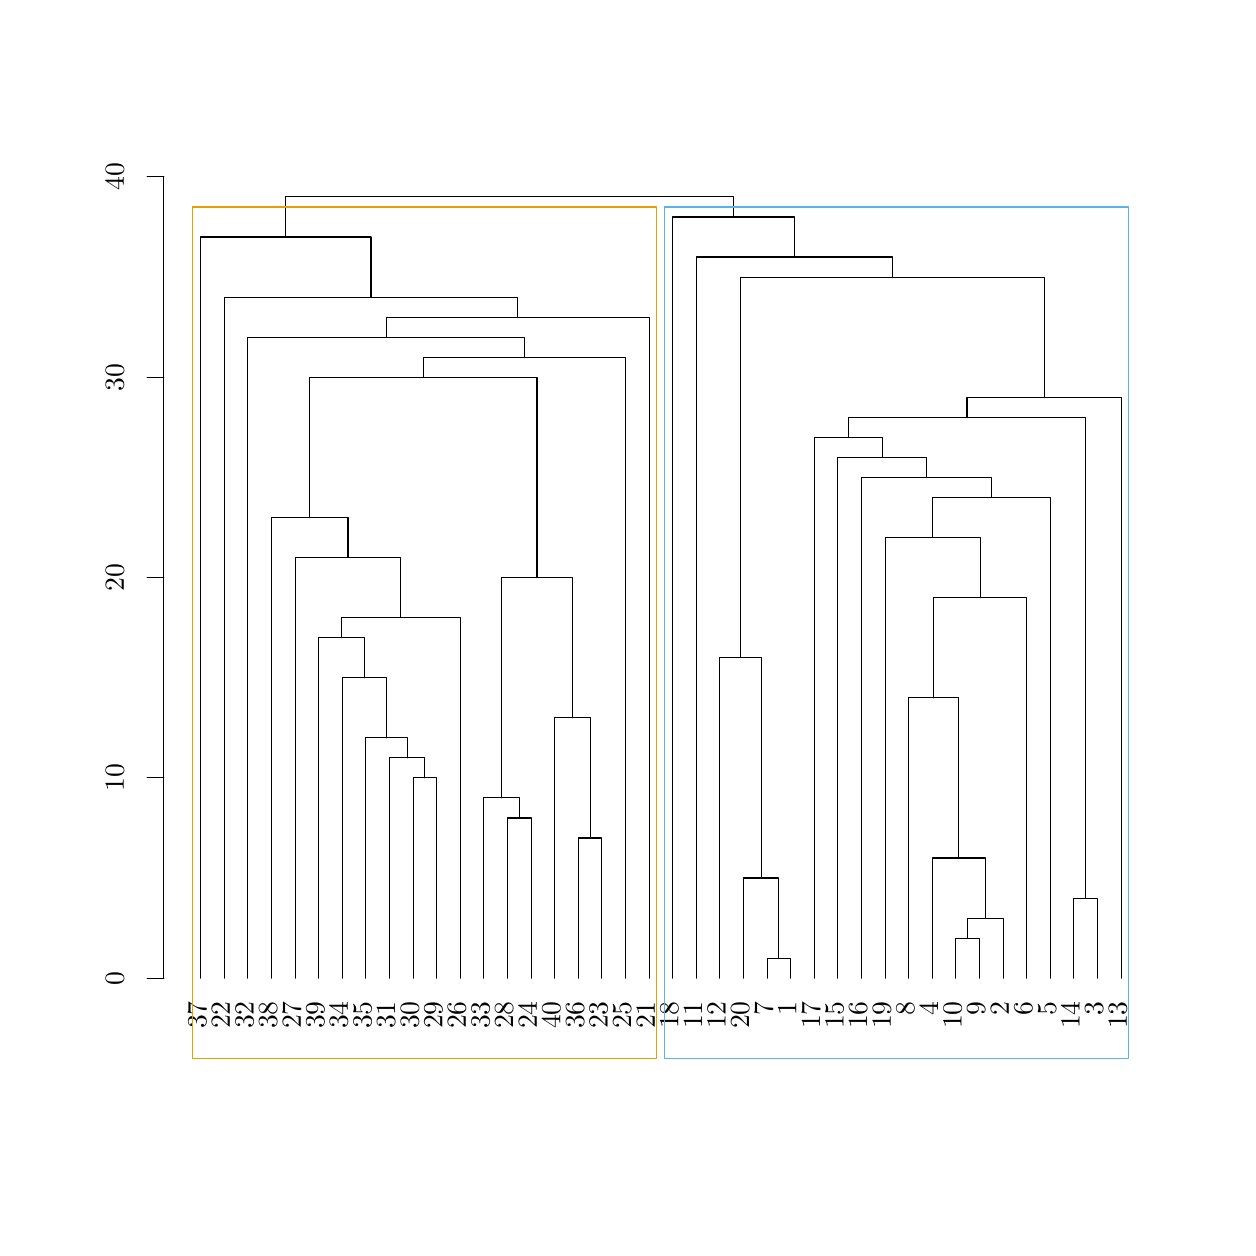
\begin{tikzpicture}[x=1pt,y=1pt]
\definecolor{fillColor}{RGB}{255,255,255}
\path[use as bounding box,fill=fillColor,fill opacity=0.00] (0,0) rectangle (433.62,433.62);
\begin{scope}
\path[clip] (  0.00,  0.00) rectangle (433.62,433.62);
\definecolor{drawColor}{RGB}{0,0,0}

\node[text=drawColor,rotate= 90.00,anchor=base east,inner sep=0pt, outer sep=0pt, scale=  1.00] at ( 64.57, 81.81) {37};

\node[text=drawColor,rotate= 90.00,anchor=base east,inner sep=0pt, outer sep=0pt, scale=  1.00] at ( 73.10, 81.81) {22};

\node[text=drawColor,rotate= 90.00,anchor=base east,inner sep=0pt, outer sep=0pt, scale=  1.00] at ( 81.63, 81.81) {32};

\node[text=drawColor,rotate= 90.00,anchor=base east,inner sep=0pt, outer sep=0pt, scale=  1.00] at ( 90.16, 81.81) {38};

\node[text=drawColor,rotate= 90.00,anchor=base east,inner sep=0pt, outer sep=0pt, scale=  1.00] at ( 98.68, 81.81) {27};

\node[text=drawColor,rotate= 90.00,anchor=base east,inner sep=0pt, outer sep=0pt, scale=  1.00] at (107.21, 81.81) {39};

\node[text=drawColor,rotate= 90.00,anchor=base east,inner sep=0pt, outer sep=0pt, scale=  1.00] at (115.74, 81.81) {34};

\node[text=drawColor,rotate= 90.00,anchor=base east,inner sep=0pt, outer sep=0pt, scale=  1.00] at (124.27, 81.81) {35};

\node[text=drawColor,rotate= 90.00,anchor=base east,inner sep=0pt, outer sep=0pt, scale=  1.00] at (132.80, 81.81) {31};

\node[text=drawColor,rotate= 90.00,anchor=base east,inner sep=0pt, outer sep=0pt, scale=  1.00] at (141.33, 81.81) {30};

\node[text=drawColor,rotate= 90.00,anchor=base east,inner sep=0pt, outer sep=0pt, scale=  1.00] at (149.86, 81.81) {29};

\path[draw=drawColor,line width= 0.4pt,line join=round,line cap=round] (139.26, 90.14) --
	(139.26,162.53) --
	(147.79,162.53) --
	(147.79, 90.14);

\path[draw=drawColor,line width= 0.4pt,line join=round,line cap=round] (130.73, 90.14) --
	(130.73,169.77) --
	(143.53,169.77) --
	(143.53,162.53);

\path[draw=drawColor,line width= 0.4pt,line join=round,line cap=round] (122.20, 90.14) --
	(122.20,177.01) --
	(137.13,177.01) --
	(137.13,169.77);

\path[draw=drawColor,line width= 0.4pt,line join=round,line cap=round] (113.68, 90.14) --
	(113.68,198.72) --
	(129.67,198.72) --
	(129.67,177.01);

\path[draw=drawColor,line width= 0.4pt,line join=round,line cap=round] (105.15, 90.14) --
	(105.15,213.20) --
	(121.67,213.20) --
	(121.67,198.72);

\node[text=drawColor,rotate= 90.00,anchor=base east,inner sep=0pt, outer sep=0pt, scale=  1.00] at (158.38, 81.81) {26};

\path[draw=drawColor,line width= 0.4pt,line join=round,line cap=round] (113.41,213.20) --
	(113.41,220.44) --
	(156.32,220.44) --
	(156.32, 90.14);

\path[draw=drawColor,line width= 0.4pt,line join=round,line cap=round] ( 96.62, 90.14) --
	( 96.62,242.15) --
	(134.86,242.15) --
	(134.86,220.44);

\path[draw=drawColor,line width= 0.4pt,line join=round,line cap=round] ( 88.09, 90.14) --
	( 88.09,256.63) --
	(115.74,256.63) --
	(115.74,242.15);

\node[text=drawColor,rotate= 90.00,anchor=base east,inner sep=0pt, outer sep=0pt, scale=  1.00] at (166.91, 81.81) {33};

\node[text=drawColor,rotate= 90.00,anchor=base east,inner sep=0pt, outer sep=0pt, scale=  1.00] at (175.44, 81.81) {28};

\node[text=drawColor,rotate= 90.00,anchor=base east,inner sep=0pt, outer sep=0pt, scale=  1.00] at (183.97, 81.81) {24};

\path[draw=drawColor,line width= 0.4pt,line join=round,line cap=round] (173.37, 90.14) --
	(173.37,148.05) --
	(181.90,148.05) --
	(181.90, 90.14);

\path[draw=drawColor,line width= 0.4pt,line join=round,line cap=round] (164.85, 90.14) --
	(164.85,155.29) --
	(177.64,155.29) --
	(177.64,148.05);

\node[text=drawColor,rotate= 90.00,anchor=base east,inner sep=0pt, outer sep=0pt, scale=  1.00] at (192.50, 81.81) {40};

\node[text=drawColor,rotate= 90.00,anchor=base east,inner sep=0pt, outer sep=0pt, scale=  1.00] at (201.03, 81.81) {36};

\node[text=drawColor,rotate= 90.00,anchor=base east,inner sep=0pt, outer sep=0pt, scale=  1.00] at (209.55, 81.81) {23};

\path[draw=drawColor,line width= 0.4pt,line join=round,line cap=round] (198.96, 90.14) --
	(198.96,140.81) --
	(207.49,140.81) --
	(207.49, 90.14);

\path[draw=drawColor,line width= 0.4pt,line join=round,line cap=round] (190.43, 90.14) --
	(190.43,184.24) --
	(203.22,184.24) --
	(203.22,140.81);

\path[draw=drawColor,line width= 0.4pt,line join=round,line cap=round] (171.24,155.29) --
	(171.24,234.91) --
	(196.83,234.91) --
	(196.83,184.24);

\path[draw=drawColor,line width= 0.4pt,line join=round,line cap=round] (101.92,256.63) --
	(101.92,307.30) --
	(184.04,307.30) --
	(184.04,234.91);

\node[text=drawColor,rotate= 90.00,anchor=base east,inner sep=0pt, outer sep=0pt, scale=  1.00] at (218.08, 81.81) {25};

\path[draw=drawColor,line width= 0.4pt,line join=round,line cap=round] (142.98,307.30) --
	(142.98,314.54) --
	(216.02,314.54) --
	(216.02, 90.14);

\path[draw=drawColor,line width= 0.4pt,line join=round,line cap=round] ( 79.56, 90.14) --
	( 79.56,321.78) --
	(179.50,321.78) --
	(179.50,314.54);

\node[text=drawColor,rotate= 90.00,anchor=base east,inner sep=0pt, outer sep=0pt, scale=  1.00] at (226.61, 81.81) {21};

\path[draw=drawColor,line width= 0.4pt,line join=round,line cap=round] (129.53,321.78) --
	(129.53,329.02) --
	(224.55,329.02) --
	(224.55, 90.14);

\path[draw=drawColor,line width= 0.4pt,line join=round,line cap=round] ( 71.03, 90.14) --
	( 71.03,336.26) --
	(177.04,336.26) --
	(177.04,329.02);

\path[draw=drawColor,line width= 0.4pt,line join=round,line cap=round] ( 62.50, 90.14) --
	( 62.50,357.97) --
	(124.04,357.97) --
	(124.04,336.26);

\node[text=drawColor,rotate= 90.00,anchor=base east,inner sep=0pt, outer sep=0pt, scale=  1.00] at (235.14, 81.81) {18};

\node[text=drawColor,rotate= 90.00,anchor=base east,inner sep=0pt, outer sep=0pt, scale=  1.00] at (243.67, 81.81) {11};

\node[text=drawColor,rotate= 90.00,anchor=base east,inner sep=0pt, outer sep=0pt, scale=  1.00] at (252.20, 81.81) {12};

\node[text=drawColor,rotate= 90.00,anchor=base east,inner sep=0pt, outer sep=0pt, scale=  1.00] at (260.73, 81.81) {20};

\node[text=drawColor,rotate= 90.00,anchor=base east,inner sep=0pt, outer sep=0pt, scale=  1.00] at (269.25, 81.81) {7};

\node[text=drawColor,rotate= 90.00,anchor=base east,inner sep=0pt, outer sep=0pt, scale=  1.00] at (277.78, 81.81) {1};

\path[draw=drawColor,line width= 0.4pt,line join=round,line cap=round] (267.19, 90.14) --
	(267.19, 97.38) --
	(275.72, 97.38) --
	(275.72, 90.14);

\path[draw=drawColor,line width= 0.4pt,line join=round,line cap=round] (258.66, 90.14) --
	(258.66,126.34) --
	(271.45,126.34) --
	(271.45, 97.38);

\path[draw=drawColor,line width= 0.4pt,line join=round,line cap=round] (250.13, 90.14) --
	(250.13,205.96) --
	(265.06,205.96) --
	(265.06,126.34);

\node[text=drawColor,rotate= 90.00,anchor=base east,inner sep=0pt, outer sep=0pt, scale=  1.00] at (286.31, 81.81) {17};

\node[text=drawColor,rotate= 90.00,anchor=base east,inner sep=0pt, outer sep=0pt, scale=  1.00] at (294.84, 81.81) {15};

\node[text=drawColor,rotate= 90.00,anchor=base east,inner sep=0pt, outer sep=0pt, scale=  1.00] at (303.37, 81.81) {16};

\node[text=drawColor,rotate= 90.00,anchor=base east,inner sep=0pt, outer sep=0pt, scale=  1.00] at (311.90, 81.81) {19};

\node[text=drawColor,rotate= 90.00,anchor=base east,inner sep=0pt, outer sep=0pt, scale=  1.00] at (320.43, 81.81) {8};

\node[text=drawColor,rotate= 90.00,anchor=base east,inner sep=0pt, outer sep=0pt, scale=  1.00] at (328.95, 81.81) {4};

\node[text=drawColor,rotate= 90.00,anchor=base east,inner sep=0pt, outer sep=0pt, scale=  1.00] at (337.48, 81.81) {10};

\node[text=drawColor,rotate= 90.00,anchor=base east,inner sep=0pt, outer sep=0pt, scale=  1.00] at (346.01, 81.81) {9};

\path[draw=drawColor,line width= 0.4pt,line join=round,line cap=round] (335.42, 90.14) --
	(335.42,104.62) --
	(343.94,104.62) --
	(343.94, 90.14);

\node[text=drawColor,rotate= 90.00,anchor=base east,inner sep=0pt, outer sep=0pt, scale=  1.00] at (354.54, 81.81) {2};

\path[draw=drawColor,line width= 0.4pt,line join=round,line cap=round] (339.68,104.62) --
	(339.68,111.86) --
	(352.47,111.86) --
	(352.47, 90.14);

\path[draw=drawColor,line width= 0.4pt,line join=round,line cap=round] (326.89, 90.14) --
	(326.89,133.57) --
	(346.08,133.57) --
	(346.08,111.86);

\path[draw=drawColor,line width= 0.4pt,line join=round,line cap=round] (318.36, 90.14) --
	(318.36,191.48) --
	(336.48,191.48) --
	(336.48,133.57);

\node[text=drawColor,rotate= 90.00,anchor=base east,inner sep=0pt, outer sep=0pt, scale=  1.00] at (363.07, 81.81) {6};

\path[draw=drawColor,line width= 0.4pt,line join=round,line cap=round] (327.42,191.48) --
	(327.42,227.68) --
	(361.00,227.68) --
	(361.00, 90.14);

\path[draw=drawColor,line width= 0.4pt,line join=round,line cap=round] (309.83, 90.14) --
	(309.83,249.39) --
	(344.21,249.39) --
	(344.21,227.68);

\node[text=drawColor,rotate= 90.00,anchor=base east,inner sep=0pt, outer sep=0pt, scale=  1.00] at (371.60, 81.81) {5};

\path[draw=drawColor,line width= 0.4pt,line join=round,line cap=round] (327.02,249.39) --
	(327.02,263.87) --
	(369.53,263.87) --
	(369.53, 90.14);

\path[draw=drawColor,line width= 0.4pt,line join=round,line cap=round] (301.30, 90.14) --
	(301.30,271.11) --
	(348.28,271.11) --
	(348.28,263.87);

\path[draw=drawColor,line width= 0.4pt,line join=round,line cap=round] (292.77, 90.14) --
	(292.77,278.35) --
	(324.79,278.35) --
	(324.79,271.11);

\path[draw=drawColor,line width= 0.4pt,line join=round,line cap=round] (284.25, 90.14) --
	(284.25,285.59) --
	(308.78,285.59) --
	(308.78,278.35);

\node[text=drawColor,rotate= 90.00,anchor=base east,inner sep=0pt, outer sep=0pt, scale=  1.00] at (380.12, 81.81) {14};

\node[text=drawColor,rotate= 90.00,anchor=base east,inner sep=0pt, outer sep=0pt, scale=  1.00] at (388.65, 81.81) {3};

\path[draw=drawColor,line width= 0.4pt,line join=round,line cap=round] (378.06, 90.14) --
	(378.06,119.10) --
	(386.59,119.10) --
	(386.59, 90.14);

\path[draw=drawColor,line width= 0.4pt,line join=round,line cap=round] (296.51,285.59) --
	(296.51,292.82) --
	(382.32,292.82) --
	(382.32,119.10);

\node[text=drawColor,rotate= 90.00,anchor=base east,inner sep=0pt, outer sep=0pt, scale=  1.00] at (397.18, 81.81) {13};

\path[draw=drawColor,line width= 0.4pt,line join=round,line cap=round] (339.42,292.82) --
	(339.42,300.06) --
	(395.12,300.06) --
	(395.12, 90.14);

\path[draw=drawColor,line width= 0.4pt,line join=round,line cap=round] (257.59,205.96) --
	(257.59,343.49) --
	(367.27,343.49) --
	(367.27,300.06);

\path[draw=drawColor,line width= 0.4pt,line join=round,line cap=round] (241.60, 90.14) --
	(241.60,350.73) --
	(312.43,350.73) --
	(312.43,343.49);

\path[draw=drawColor,line width= 0.4pt,line join=round,line cap=round] (233.07, 90.14) --
	(233.07,365.21) --
	(277.02,365.21) --
	(277.02,350.73);

\path[draw=drawColor,line width= 0.4pt,line join=round,line cap=round] ( 93.27,357.97) --
	( 93.27,372.45) --
	(255.05,372.45) --
	(255.05,365.21);
\end{scope}
\begin{scope}
\path[clip] (  0.00,  0.00) rectangle (433.62,433.62);
\definecolor{drawColor}{RGB}{0,0,0}

\path[draw=drawColor,line width= 0.4pt,line join=round,line cap=round] ( 49.20, 90.14) -- ( 49.20,379.69);

\path[draw=drawColor,line width= 0.4pt,line join=round,line cap=round] ( 49.20, 90.14) -- ( 43.20, 90.14);

\path[draw=drawColor,line width= 0.4pt,line join=round,line cap=round] ( 49.20,162.53) -- ( 43.20,162.53);

\path[draw=drawColor,line width= 0.4pt,line join=round,line cap=round] ( 49.20,234.91) -- ( 43.20,234.91);

\path[draw=drawColor,line width= 0.4pt,line join=round,line cap=round] ( 49.20,307.30) -- ( 43.20,307.30);

\path[draw=drawColor,line width= 0.4pt,line join=round,line cap=round] ( 49.20,379.69) -- ( 43.20,379.69);

\node[text=drawColor,rotate= 90.00,anchor=base,inner sep=0pt, outer sep=0pt, scale=  1.00] at ( 34.80, 90.14) {0};

\node[text=drawColor,rotate= 90.00,anchor=base,inner sep=0pt, outer sep=0pt, scale=  1.00] at ( 34.80,162.53) {10};

\node[text=drawColor,rotate= 90.00,anchor=base,inner sep=0pt, outer sep=0pt, scale=  1.00] at ( 34.80,234.91) {20};

\node[text=drawColor,rotate= 90.00,anchor=base,inner sep=0pt, outer sep=0pt, scale=  1.00] at ( 34.80,307.30) {30};

\node[text=drawColor,rotate= 90.00,anchor=base,inner sep=0pt, outer sep=0pt, scale=  1.00] at ( 34.80,379.69) {40};
\end{scope}
\begin{scope}
\path[clip] ( 49.20, 61.20) rectangle (408.42,384.42);
\definecolor{drawColor}{RGB}{230,159,0}

\path[draw=drawColor,line width= 0.4pt,line join=round,line cap=round] ( 59.60, 61.20) rectangle (227.36,368.83);
\definecolor{drawColor}{RGB}{86,180,233}

\path[draw=drawColor,line width= 0.4pt,line join=round,line cap=round] (230.17, 61.20) rectangle (397.93,368.83);
\end{scope}
\end{tikzpicture}

	\caption{Dendogram Girvan-Newman method for community detection}
	\label{p10}
\end{figure}

\end{document}
